\documentclass[10pt]{article}
\usepackage[margin=0.68in]{geometry}
\usepackage[T1]{fontenc}
\usepackage[utf8]{inputenc}
\usepackage{lmodern}
\usepackage{amsmath,amssymb,mathtools}
\usepackage{xcolor}
\usepackage{hyperref}
\usepackage{fancyhdr}
\usepackage{titlesec}
\usepackage{enumitem}
\usepackage{longtable}
\usepackage{tabularx}
\usepackage{booktabs}
\usepackage{adjustbox}
\usepackage{fancyvrb}
\usepackage{tikz}
\usetikzlibrary{arrows.meta,positioning,shapes.geometric,calc}
\definecolor{navy}{HTML}{0C2744}
\definecolor{blue}{HTML}{1E63E9}
\definecolor{cyan}{HTML}{1DB6C7}
\definecolor{paper}{HTML}{F4F7FB}
\definecolor{green}{HTML}{167A5B}
\definecolor{amber}{HTML}{B77700}
\hypersetup{colorlinks=true,linkcolor=blue,urlcolor=blue,pdftitle={AI Engineering Interview Atlas}}
\pagestyle{fancy}\fancyhf{}\fancyhead[L]{\textcolor{navy}{AI Engineering Interview Atlas}}\fancyhead[R]{\textcolor{gray}{\leftmark}}\fancyfoot[C]{\thepage}
\titleformat{\section}{\Large\bfseries\color{navy}}{\thesection}{.7em}{}
\titleformat{\subsection}{\large\bfseries\color{blue}}{\thesubsection}{.7em}{}
\titleformat{\subsubsection}{\normalsize\bfseries\color{navy}}{\thesubsubsection}{.7em}{}
\setlist{nosep,leftmargin=*}
\setlength{\parindent}{0pt}
\setlength{\parskip}{3pt}
\newcommand{\tradeoff}[1]{\par\smallskip\noindent\textbf{Tradeoff.} #1}
\newcommand{\pitfall}[1]{\par\smallskip\noindent\textbf{Production failure.} #1}
\newcommand{\badge}[1]{\colorbox{paper}{\textcolor{blue}{\textbf{#1}}}}
\newcommand{\mathblock}[1]{\begin{center}\begin{adjustbox}{max width=\linewidth}$\displaystyle #1$\end{adjustbox}\end{center}}
\newenvironment{derivation}{\begin{quote}\small\color{navy}}{\end{quote}}
\begin{document}
\begin{titlepage}\pagecolor{navy}\color{white}\vspace*{1.1in}{\Huge\bfseries AI Engineering\\Interview Atlas\par}\vspace{.4in}{\Large Systems, theory, and 1,000+ questions\par}\vfill{\large Research snapshot: 2 September 2026\par}\vspace{.15in}{\normalsize Primary papers, official documentation, specifications, and standards\par}\vspace{.7in}{\color{cyan}\rule{\textwidth}{3pt}}\end{titlepage}\nopagecolor\color{black}
\tableofcontents\newpage
\section{How to use this handbook}
This handbook contains 192 topic notes, 1920 generated practice questions, 50 core interview questions, and 12 progressive system-design challenges. Study mechanisms first, state tradeoffs second, then describe measurement, failure handling, and rollback.
\subsection{Curriculum architecture}
\begin{center}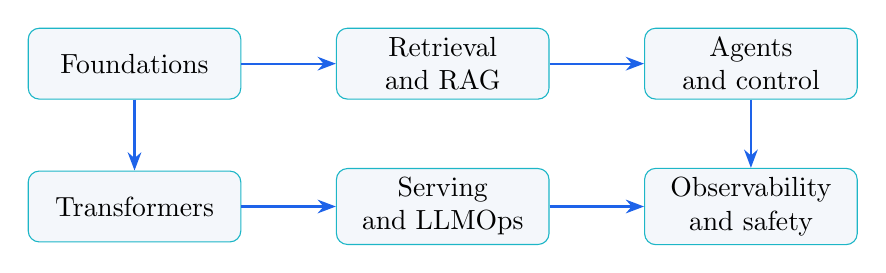
\begin{tikzpicture}[node distance=9mm and 12mm,box/.style={draw=cyan,fill=paper,rounded corners,align=center,minimum width=27mm,minimum height=9mm},arr/.style={-{Stealth},thick,draw=blue}]\node[box](f){Foundations};\node[box,right=of f](r){Retrieval\\and RAG};\node[box,right=of r](a){Agents\\and control};\node[box,below=of f](t){Transformers};\node[box,right=of t](s){Serving\\and LLMOps};\node[box,right=of s](o){Observability\\and safety};\draw[arr](f)--(r);\draw[arr](r)--(a);\draw[arr](f)--(t);\draw[arr](t)--(s);\draw[arr](s)--(o);\draw[arr](a)--(o);\end{tikzpicture}\end{center}
\section{Retrieval and Search Theory}
\subsection{BM25}
A probabilistic lexical ranker that rewards term frequency while saturating repeated terms and normalizing document length.
\tradeoff{It is fast, interpretable, and exact for rare tokens but cannot directly match paraphrases.}
\pitfall{Treating it as obsolete removes a strong baseline and hurts identifier-heavy queries.}
\subsection{TF-IDF}
A sparse weighting scheme that combines within-document frequency with inverse collection frequency.
\tradeoff{It is transparent and cheap but lacks BM25's term-frequency saturation and tuned length normalization.}
\pitfall{Comparing raw cosine scores across changing corpora without rebuilding IDF causes drift.}
\subsection{Dense retrieval}
A bi-encoder maps queries and passages into a shared embedding space for nearest-neighbor search.
\tradeoff{Semantic recall improves, while exact names, numbers, and out-of-domain language may regress.}
\pitfall{Evaluating only on in-domain examples hides lexical misses and embedding drift.}
\subsection{Sparse neural retrieval}
Learned sparse models retain token-aligned inverted-index retrieval while expanding or reweighting terms.
\tradeoff{They bridge lexical and semantic matching but increase index size and model cost.}
\pitfall{Unbounded expansion creates latency and storage blowups.}
\subsection{Late interaction}
ColBERT-style systems preserve token-level embeddings and aggregate fine-grained similarities at query time.
\tradeoff{Accuracy often beats single-vector retrieval, with a larger index and heavier scoring path.}
\pitfall{Treating a late-interaction index like one-vector-per-document underestimates capacity needs.}
\subsection{Cross-encoder reranking}
A model jointly encodes query and candidate text to assign a relevance score.
\tradeoff{It gives strong precision on a small candidate set but is too expensive for full-corpus retrieval.}
\pitfall{Reranking too many long passages dominates p95 latency.}
\subsection{Hybrid retrieval}
Dense and lexical signals are retrieved together and fused, often with weighted scores or reciprocal-rank fusion.
\tradeoff{It improves robustness across semantic and exact-match queries but requires score calibration and duplicate handling.}
\pitfall{Adding incomparable raw scores without normalization makes one retriever dominate.}
\subsection{Reciprocal rank fusion}
RRF combines ranked lists using reciprocal rank positions rather than raw score scales.
\tradeoff{It is robust without score calibration but ignores the magnitude and confidence of scores.}
\pitfall{Using an overly small rank constant can overreward noisy top results.}
\subsection{ANN recall}
Approximate nearest-neighbor recall measures how many true nearest items are recovered by an index configuration.
\tradeoff{Higher recall usually costs memory, build time, or query latency.}
\pitfall{Reporting application answer quality without measuring index recall hides retrieval infrastructure defects.}
\subsection{Retrieval metrics}
Recall@k, precision@k, MRR, MAP, and nDCG measure different ranking behaviors.
\tradeoff{A metric must match the product objective and judgment granularity.}
\pitfall{Optimizing MRR for a task that consumes many passages can worsen context coverage.}
\subsection{Embedding geometry}
Similarity functions, normalization, anisotropy, dimensionality, and training objectives shape neighborhood quality.
\tradeoff{Cosine, dot product, and Euclidean distance can be equivalent only under specific normalization assumptions.}
\pitfall{Mixing an index metric with a differently trained embedding objective silently harms ranking.}
\subsection{Query expansion}
Expansion adds synonyms, generated subqueries, or pseudo-relevance terms before retrieval.
\tradeoff{Recall can improve at the expense of latency and topic drift.}
\pitfall{Letting an LLM expand unconstrained queries can inject unsupported intent.}
\section{Vector Databases and Search Engines}
\subsection{pgvector}
A PostgreSQL extension that stores vectors beside relational data and supports exact, HNSW, and IVFFlat search.
\tradeoff{It simplifies transactions and joins, while specialized stores may scale independent vector workloads more easily.}
\pitfall{Adding an ANN index without tuning filtering and planner behavior can reduce recall or miss the index.}
\subsection{Pinecone}
A managed vector service with metadata filtering, namespaces, and dense-sparse hybrid retrieval.
\tradeoff{Operations are outsourced, trading infrastructure control and portability for managed scale.}
\pitfall{Poor namespace and metadata design creates noisy tenants and expensive fan-out queries.}
\subsection{Qdrant}
An open-source vector engine centered on HNSW, payload filtering, quantization, and distributed collections.
\tradeoff{It offers operational control and rich filtering but adds a stateful distributed service to run.}
\pitfall{Applying post-filtering after ANN can return too few eligible results.}
\subsection{Weaviate}
A vector database with collections, hybrid search, filters, modules, and multi-tenancy features.
\tradeoff{An integrated schema accelerates product work but may couple ingestion and inference choices.}
\pitfall{Automatic vectorization without explicit model version metadata makes reindexing unsafe.}
\subsection{Milvus and Zilliz}
Milvus is a distributed vector database; Zilliz provides its managed service with multiple index choices.
\tradeoff{It targets large-scale separation of compute and storage, with more operational concepts than embedded options.}
\pitfall{Selecting an index by popularity instead of dataset size and latency-recall tests wastes resources.}
\subsection{Elasticsearch vector search}
Elasticsearch combines inverted indexes, filters, aggregations, and approximate kNN in one search platform.
\tradeoff{It is compelling for existing Elastic estates but vector memory and shard design require care.}
\pitfall{Oversharding fragments candidate pools and increases coordination overhead.}
\subsection{OpenSearch vector search}
OpenSearch supports lexical and vector workloads with pluggable kNN engines and search pipelines.
\tradeoff{Open governance and integrated search are attractive, while engine-specific behavior complicates tuning.}
\pitfall{Assuming identical parameters across FAISS, Lucene, and NMSLIB backends produces misleading tests.}
\subsection{Redis vector search}
Redis Query Engine adds vector indexes and filters to an in-memory data platform.
\tradeoff{Very low latency is possible, but RAM cost and persistence design matter at scale.}
\pitfall{Using Redis only as a vector database without capacity planning can evict critical data.}
\subsection{Chroma}
Chroma is a developer-oriented embedding store commonly used for local prototypes and small applications.
\tradeoff{It favors simplicity and iteration speed over complex distributed operations.}
\pitfall{Promoting a local prototype topology directly to production skips backup, tenancy, and load tests.}
\subsection{LanceDB}
LanceDB uses a columnar, versioned data format and supports vector, full-text, and multimodal data locally or in cloud storage.
\tradeoff{It fits data-lake and embedded workflows but differs operationally from a server-first database.}
\pitfall{Ignoring compaction and version retention can degrade read performance and inflate storage.}
\subsection{Vespa}
Vespa combines structured filtering, lexical search, tensors, ranking functions, and online serving.
\tradeoff{It enables sophisticated multi-stage ranking but has a steeper schema and operations learning curve.}
\pitfall{Putting expensive ranking expressions in the first phase can collapse throughput.}
\subsection{HNSW}
A navigable multilayer proximity graph controlled by construction degree and search breadth.
\tradeoff{It offers strong latency-recall behavior with significant memory and build cost.}
\pitfall{Deleting or heavily filtering data without maintenance degrades graph quality.}
\subsection{IVF and PQ}
Inverted files narrow the search to clusters; product quantization compresses vectors for cheaper approximate scoring.
\tradeoff{Memory and latency fall, while training quality and quantization error reduce recall.}
\pitfall{Training centroids or codebooks on an unrepresentative sample bakes bias into the index.}
\subsection{Metadata filtering}
Attribute constraints restrict eligible vectors before, during, or after ANN search.
\tradeoff{Early filtering preserves relevance but can make graph traversal sparse; post-filtering may underfill results.}
\pitfall{Failing to test selective filters separately from unfiltered queries hides severe recall loss.}
\section{RAG Architecture and Evaluation}
\subsection{Document ingestion}
Ingestion parses, normalizes, classifies, deduplicates, and records provenance before indexing.
\tradeoff{Rich preprocessing improves retrieval but increases pipeline cost and reprocessing complexity.}
\pitfall{Losing stable document and chunk identifiers makes updates create duplicates.}
\subsection{Chunking}
Chunking chooses semantic units, size, overlap, and metadata boundaries for retrieval and context assembly.
\tradeoff{Smaller chunks improve precision; larger chunks preserve context and reduce fragmentation.}
\pitfall{Fixed-size splitting across tables, code, or headings destroys meaning.}
\subsection{Parent-child retrieval}
Small child chunks retrieve precisely while larger parent sections are supplied to the model.
\tradeoff{It separates retrieval granularity from generation context at extra storage and mapping cost.}
\pitfall{Returning many overlapping parents wastes context and amplifies one source.}
\subsection{Contextual compression}
A post-retrieval step extracts or rewrites only query-relevant evidence from candidates.
\tradeoff{It saves context tokens but can delete qualifiers or introduce summarization errors.}
\pitfall{Using the same weak model for compression and answering creates correlated failures.}
\subsection{Query routing}
A router chooses retrievers, indexes, tools, or no-retrieval paths based on intent and risk.
\tradeoff{Specialization improves quality and cost but adds classification errors and operational branches.}
\pitfall{A route without confidence or fallback turns ambiguous queries into hard failures.}
\subsection{Multi-query retrieval}
The system generates several query formulations and merges their result sets.
\tradeoff{Recall rises at the cost of additional searches, duplicates, and possible intent drift.}
\pitfall{Treating all generated queries as equally trustworthy invites off-topic evidence.}
\subsection{HyDE}
Hypothetical Document Embeddings generate a likely answer passage and embed it as the retrieval query.
\tradeoff{It can bridge terse questions to document style but may anchor retrieval on invented details.}
\pitfall{Passing the hypothetical text to generation as evidence confuses a retrieval aid with a source.}
\subsection{Reranking pipeline}
A staged ranker retrieves broadly, applies filters, reranks candidates, and packs final context.
\tradeoff{More stages improve control but add latency, failure modes, and tuning surfaces.}
\pitfall{Evaluating only final answers makes it hard to locate which stage regressed.}
\subsection{Context packing}
Packing selects, orders, deduplicates, and labels evidence within a token budget.
\tradeoff{Diversity and source coverage compete with local relevance and continuity.}
\pitfall{Greedy top-score packing often repeats one document and crowds out complementary facts.}
\subsection{Grounded generation}
Prompts and decoding require answers to use cited evidence and abstain when evidence is insufficient.
\tradeoff{Strong grounding can reduce creativity and answer rate while improving auditability.}
\pitfall{A citation marker is not proof that the cited text entails the claim.}
\subsection{RAG evaluation}
Retrieval, context, generation, citation, latency, and cost require separate offline and online measures.
\tradeoff{Automated judges accelerate iteration but need human calibration and bias checks.}
\pitfall{Collapsing all dimensions into one score hides compensating failures.}
\subsection{Faithfulness}
Faithfulness asks whether claims in an answer are supported by the supplied context.
\tradeoff{It is narrower and more testable than global factuality but depends on context quality.}
\pitfall{Marking unsupported common knowledge as grounded inflates results.}
\subsection{Answer relevance}
Answer relevance measures whether a response directly addresses the user question without unnecessary content.
\tradeoff{Concision may improve relevance while losing useful caveats.}
\pitfall{A fluent on-topic answer can still be factually wrong, so relevance cannot stand alone.}
\subsection{Synthetic test generation}
Models generate questions, expected evidence, and variants from a source corpus to expand evaluation coverage.
\tradeoff{Coverage grows cheaply, while generator bias and leakage can make the benchmark too easy.}
\pitfall{Testing with the same model family that authored the cases can overstate quality.}
\subsection{Online RAG monitoring}
Production monitoring tracks retrieval gaps, unsupported claims, drift, feedback, latency, and cost by slice.
\tradeoff{Rich telemetry improves diagnosis but raises privacy and storage obligations.}
\pitfall{Logging full prompts and context without redaction can expose sensitive data.}
\section{Knowledge Graphs and GraphRAG}
\subsection{Property graphs}
Nodes, typed relationships, and properties represent entities and their connections for traversal and pattern matching.
\tradeoff{They are intuitive for operational queries but semantics depend on disciplined labels and schema.}
\pitfall{Using untyped generic edges turns the graph into an expensive document store.}
\subsection{RDF and ontologies}
RDF triples plus vocabularies such as RDFS or OWL provide globally identified semantics and inference rules.
\tradeoff{Formal interoperability grows, with more modeling and reasoning complexity.}
\pitfall{Confusing open-world semantics with database constraints produces invalid assumptions.}
\subsection{Cypher}
Cypher expresses graph patterns, predicates, paths, updates, and aggregation for property graphs.
\tradeoff{Declarative queries are readable, while unbounded path patterns can be expensive.}
\pitfall{Omitting labels or relationship types can trigger broad scans.}
\subsection{Knowledge graph construction}
Construction extracts entities and relations, resolves identities, applies schema, validates facts, and records provenance.
\tradeoff{Automation scales coverage but introduces extraction and entity-resolution errors.}
\pitfall{Allowing generated edges without source spans prevents later verification.}
\subsection{Entity resolution}
Entity resolution links mentions and records that refer to the same real-world entity.
\tradeoff{Aggressive merging improves connectivity but risks catastrophic false joins.}
\pitfall{Matching on names alone fails for aliases, homonyms, and temporal identity changes.}
\subsection{GraphRAG local search}
Local search expands from query-relevant entities through nearby relationships and associated text.
\tradeoff{It supports entity-centric multi-hop questions but depends on extraction and linking quality.}
\pitfall{Unbounded neighborhood expansion floods context with high-degree hubs.}
\subsection{GraphRAG global search}
Global search summarizes graph communities and combines relevant community reports for corpus-level questions.
\tradeoff{It addresses whole-corpus themes but has expensive indexing and lossy summaries.}
\pitfall{Expecting global search to answer precise record lookups wastes cost and may lose detail.}
\subsection{KAG}
Knowledge Augmented Generation combines schema-aware graphs, chunk mutual indexing, alignment, and logical-form-guided reasoning.
\tradeoff{It improves domain logic and multi-hop control at substantial modeling and maintenance cost.}
\pitfall{Adopting KAG without stable domain schema simply relocates ambiguity.}
\subsection{Graph quality evaluation}
Evaluation checks entity precision, relation correctness, completeness, consistency, provenance, and downstream QA value.
\tradeoff{Intrinsic graph metrics catch construction defects but may not predict application utility.}
\pitfall{Reporting only downstream answer scores can hide a brittle graph with unverifiable facts.}
\subsection{Temporal knowledge graphs}
Facts carry validity intervals, event time, and version history so queries can reason about change.
\tradeoff{Temporal accuracy improves, while updates, conflicts, and query logic become harder.}
\pitfall{Overwriting old facts destroys the ability to answer as-of questions.}
\section{Agents, MCP, and Control}
\subsection{Agent loop}
An agent repeatedly observes state, chooses an action, invokes a tool, and incorporates the result until stopping.
\tradeoff{Flexibility handles open-ended tasks, but loop length and behavior are less predictable than workflows.}
\pitfall{Omitting hard budgets and stop conditions creates runaway calls.}
\subsection{ReAct}
ReAct interleaves reasoning with actions and observations to update plans using external evidence.
\tradeoff{Tool feedback can correct model knowledge, while longer trajectories add latency and error opportunities.}
\pitfall{Treating every thought as reliable state allows early mistakes to compound.}
\subsection{Planning}
Planning decomposes goals into ordered, conditional, or revisable steps before or during execution.
\tradeoff{Upfront plans improve structure but become stale in uncertain environments.}
\pitfall{Forcing a long immutable plan prevents recovery after new observations.}
\subsection{Reflection}
Reflection critiques outcomes or trajectories and stores actionable lessons for another attempt.
\tradeoff{It can improve recovery without weight updates, while self-critique may repeat the same bias.}
\pitfall{Saving vague reflections adds context without changing behavior.}
\subsection{Tool calling}
Models emit structured arguments for declared functions that a host validates and executes.
\tradeoff{It narrows the action interface but does not make proposed actions safe or correct.}
\pitfall{Executing model-produced arguments without schema and authorization checks invites damage.}
\subsection{Model Context Protocol}
MCP standardizes client-server discovery and invocation of tools, resources, prompts, and related capabilities.
\tradeoff{Interoperability improves, while trust boundaries, consent, and capability scoping remain host responsibilities.}
\pitfall{Treating a discovered MCP server as trusted creates prompt-injection and privilege risks.}
\subsection{Agent memory}
Working, episodic, semantic, and procedural memories preserve relevant state beyond a single model call.
\tradeoff{Memory supports continuity but retrieval, deletion, privacy, and stale facts become product concerns.}
\pitfall{Writing every interaction to long-term memory creates noise and privacy exposure.}
\subsection{Human in the loop}
High-risk actions pause for review, edit, approval, rejection, or direct human response.
\tradeoff{Oversight reduces irreversible mistakes but adds latency and reviewer load.}
\pitfall{Asking for approval after an action has already caused side effects is theater.}
\subsection{State machines}
Explicit states and transitions constrain allowed agent behavior and make recovery inspectable.
\tradeoff{Predictability and testability improve at the cost of less open-ended autonomy.}
\pitfall{Encoding side effects inside transition guards breaks replay safety.}
\subsection{Idempotent tools}
An idempotent tool can be retried with the same operation key without duplicating the intended effect.
\tradeoff{Reliable retries require deduplication state and carefully defined semantics.}
\pitfall{Assuming HTTP method alone guarantees business idempotency causes duplicate orders or messages.}
\subsection{Agent handoffs}
A handoff transfers a task and structured context to a specialized agent or deterministic service.
\tradeoff{Specialization reduces prompt overload but adds routing and ownership ambiguity.}
\pitfall{Passing the entire transcript leaks irrelevant data and confuses the recipient.}
\subsection{Autonomy levels}
Autonomy is graduated from suggest-only through approval-gated execution to bounded autonomous operation.
\tradeoff{More autonomy reduces human effort while increasing required assurance and containment.}
\pitfall{Assigning one global autonomy level ignores action-specific risk.}
\subsection{Context engineering}
Context engineering selects instructions, memory, evidence, tools, schemas, and state for each model turn.
\tradeoff{Targeted context improves reliability and cost, but selection logic becomes core application code.}
\pitfall{Appending everything causes attention dilution and instruction conflicts.}
\subsection{Sandbox runs}
A sandbox isolates untrusted code with resource limits, scoped files, network policy, timeouts, and audit logs.
\tradeoff{Isolation enables capability while imposing startup and compatibility overhead.}
\pitfall{A container without kernel, credential, and network boundaries is not a sufficient sandbox.}
\section{Orchestration Frameworks}
\subsection{LangGraph}
LangGraph models long-running agent workflows as stateful graphs with checkpoints, interrupts, streaming, and durable execution.
\tradeoff{Fine-grained control aids production reliability but exposes more state and graph design decisions.}
\pitfall{Non-idempotent node side effects make checkpoint replay unsafe.}
\subsection{LlamaIndex workflows}
Event-driven workflows coordinate retrieval, tools, agents, and structured steps in the LlamaIndex ecosystem.
\tradeoff{Strong data and indexing integrations speed RAG work but can couple application flow to framework abstractions.}
\pitfall{Hiding all retrieval behind defaults makes evaluation and migration difficult.}
\subsection{Haystack pipelines}
Haystack connects typed components into retrieval, generation, routing, and agent pipelines.
\tradeoff{Explicit components support testing, while custom graphs still require lifecycle discipline.}
\pitfall{Allowing incompatible document schemas across components creates runtime surprises.}
\subsection{PydanticAI}
PydanticAI uses typed dependencies, tools, results, and validation to build model-agnostic Python agents.
\tradeoff{Type safety improves integration but cannot validate semantic truth.}
\pitfall{Confusing schema conformance with a correct answer produces false confidence.}
\subsection{Semantic Kernel}
Semantic Kernel offers planners, agents, plugins, memory connectors, and multi-language enterprise integration.
\tradeoff{Its broad integration surface suits platform teams but introduces framework concepts and version coupling.}
\pitfall{Registering overly broad plugins grants the model unnecessary authority.}
\subsection{AutoGen}
AutoGen structures multi-agent conversations and tool-using participants for collaborative task execution.
\tradeoff{Role decomposition enables complex workflows but multiplies calls, coordination failures, and evaluation cost.}
\pitfall{Adding agents without independent capabilities creates expensive echo chambers.}
\subsection{CrewAI}
CrewAI organizes role-based agents, tasks, crews, and flows for sequential or coordinated work.
\tradeoff{It gives accessible orchestration but still needs explicit state, permissions, and observability.}
\pitfall{Persona descriptions cannot substitute for tool-level access control.}
\subsection{DSPy}
DSPy treats prompts and modules as optimizable programs evaluated against examples and metrics.
\tradeoff{Systematic optimization can beat manual prompting, while it depends on representative data and stable metrics.}
\pitfall{Optimizing against a leaky judge overfits wording instead of capability.}
\subsection{Temporal}
Temporal persists workflow history and replays deterministic workflow code around durable activities.
\tradeoff{It provides robust retries and long-running execution but requires deterministic workflow discipline.}
\pitfall{Reading wall-clock time or random state directly in replayed code causes nondeterminism.}
\subsection{Airflow, Dagster, and Prefect}
General-purpose data orchestrators schedule DAGs, assets, or flows with retries, lineage, and operational UIs.
\tradeoff{They excel at batch pipelines but are not automatically low-latency interactive agent runtimes.}
\pitfall{Running per-token or per-chat-turn work as heavy batch tasks adds unacceptable overhead.}
\section{Observability and Monitoring}
\subsection{OpenTelemetry}
OpenTelemetry provides vendor-neutral APIs, SDKs, collectors, and semantic conventions for traces, metrics, logs, and profiles.
\tradeoff{Portability improves, while instrumentation quality and backend cost remain engineering work.}
\pitfall{High-cardinality prompt or user attributes can overwhelm telemetry systems.}
\subsection{Distributed tracing}
Traces connect request spans across gateways, retrievers, models, tools, queues, and databases.
\tradeoff{They reveal critical paths but sampling can hide rare quality failures.}
\pitfall{Reusing trace identifiers across independent user requests breaks isolation.}
\subsection{LLM tracing}
LLM traces capture prompts, outputs, model settings, token usage, latency, tool calls, retrieval, and evaluations.
\tradeoff{Debugging improves, while content capture raises privacy and retention risk.}
\pitfall{Logging secrets or personal data by default creates a second sensitive datastore.}
\subsection{Metrics and SLOs}
Counters, histograms, gauges, service-level indicators, and objectives quantify reliability and performance.
\tradeoff{Aggregate signals scale well but cannot explain individual semantic failures.}
\pitfall{Averaging latency hides long-tail p95 and p99 user pain.}
\subsection{Structured logging}
Structured events use stable fields, severity, timestamps, correlation IDs, and redaction.
\tradeoff{Search and aggregation improve, while schemas must evolve consistently.}
\pitfall{Placing unbounded model output in one log field causes cost and ingestion failures.}
\subsection{LangSmith}
LangSmith provides tracing, datasets, evaluation, prompt management, and deployment-oriented tooling for LLM applications.
\tradeoff{Tight LangChain integration accelerates work but requires portability planning.}
\pitfall{Depending only on vendor UI annotations leaves evaluation logic unreproducible.}
\subsection{Langfuse}
Langfuse is an open-source platform for LLM traces, sessions, prompts, scores, datasets, and cost analytics.
\tradeoff{Self-hosting offers control but shifts scaling, upgrades, and security to the team.}
\pitfall{Capturing every token forever creates expensive sensitive retention.}
\subsection{Arize Phoenix}
Phoenix provides open-source tracing and evaluation for LLM, retrieval, and agent applications with OpenTelemetry support.
\tradeoff{It unifies qualitative traces and quantitative evals, while production operations still need design.}
\pitfall{Judge scores without slice analysis can mask failures for important cohorts.}
\subsection{MLflow tracing}
MLflow connects traces, evaluation datasets, scorers, experiments, and production monitoring.
\tradeoff{A common ML platform improves lineage but may be heavier than a focused tracing tool.}
\pitfall{Mixing incomparable scorer versions in one trend chart produces false regressions.}
\subsection{W\&B Weave}
Weave tracks calls, objects, datasets, evaluations, and model application experiments.
\tradeoff{Rich experiment lineage helps collaboration but introduces another governance surface.}
\pitfall{Saving mutable datasets without immutable versions undermines reproducibility.}
\subsection{Prompt and model drift}
Drift monitoring detects changes in inputs, retrieved evidence, outputs, model versions, and user behavior.
\tradeoff{Alerts catch regressions but thresholds must distinguish seasonality from harm.}
\pitfall{Measuring embedding distribution shift alone does not prove answer quality changed.}
\subsection{Cost observability}
Cost telemetry attributes input, output, cache, retrieval, tool, and infrastructure spend to requests and tenants.
\tradeoff{Unit economics become actionable, while provider pricing and caching rules evolve.}
\pitfall{Tracking only average cost hides pathological long-running agents.}
\subsection{Evaluation in production}
Online evaluators combine sampled judges, deterministic checks, human feedback, and business outcomes.
\tradeoff{Live coverage improves realism but evaluations must not expose or delay users.}
\pitfall{Treating implicit clicks as unambiguous quality labels creates bias.}
\section{Serving, Deployment, and LLMOps}
\subsection{vLLM}
vLLM is a high-throughput inference server using PagedAttention, continuous batching, parallelism, and OpenAI-compatible APIs.
\tradeoff{Throughput and memory utilization improve, while model and kernel compatibility must be verified.}
\pitfall{Benchmarking only one concurrency level hides latency-throughput collapse points.}
\subsection{SGLang}
SGLang combines a structured generation runtime with optimized model serving, prefix reuse, batching, and parallelism.
\tradeoff{Tight runtime-serving integration can accelerate agentic workloads but changes application abstractions.}
\pitfall{Assuming every structured program benefits equally from cache reuse leads to poor capacity models.}
\subsection{Text Generation Inference}
TGI is a Hugging Face server for transformer inference with streaming, batching, quantization, and distributed support.
\tradeoff{Ecosystem integration is strong, while supported optimization paths vary by model and hardware.}
\pitfall{Enabling quantization without quality and kernel tests can reduce both accuracy and speed.}
\subsection{TensorRT-LLM}
TensorRT-LLM compiles and serves NVIDIA-optimized LLM graphs and kernels across GPUs.
\tradeoff{Maximum NVIDIA performance comes with build complexity and hardware coupling.}
\pitfall{Rebuilding engines for every shape without a deployment cache slows releases.}
\subsection{NVIDIA Triton}
Triton serves multiple model frameworks with dynamic batching, ensembles, metrics, and model repositories.
\tradeoff{It standardizes diverse serving, though LLM-specific scheduling may require specialized backends.}
\pitfall{Using dynamic batching without queue-delay limits breaks interactive latency.}
\subsection{llama.cpp}
llama.cpp runs quantized models efficiently on CPUs and varied local accelerators through a portable C++ stack.
\tradeoff{Edge privacy and low dependency count trade off against datacenter throughput and model size.}
\pitfall{Selecting a quantization by file size alone ignores accuracy and hardware kernels.}
\subsection{KServe}
KServe provides Kubernetes-native inference services, autoscaling, revisions, traffic splitting, and model runtimes.
\tradeoff{Platform consistency improves, with Kubernetes operational overhead and cold-start concerns.}
\pitfall{Scaling only on CPU misses token queue pressure in GPU workloads.}
\subsection{Ray Serve}
Ray Serve composes Python model deployments and scales replicas across a Ray cluster.
\tradeoff{Flexible distributed Python pipelines fit multi-model systems but require cluster and object-store discipline.}
\pitfall{Passing large tensors repeatedly through serialization paths wastes memory and latency.}
\subsection{BentoML}
BentoML packages model services, dependencies, APIs, and deployment configuration with adaptive batching.
\tradeoff{Developer workflow is streamlined, while platform integration and runtime tuning still matter.}
\pitfall{Treating packaging success as load readiness skips concurrency tests.}
\subsection{Kubernetes and GPUs}
Kubernetes schedules containers and device resources while operators add GPU sharing, queues, and autoscaling.
\tradeoff{A common control plane helps governance but default scheduling is not token-aware.}
\pitfall{Requesting whole GPUs for tiny models can strand capacity.}
\subsection{LLM gateways}
Gateways normalize provider APIs and add routing, budgets, rate limits, fallbacks, caching, and audit policy.
\tradeoff{Central control improves governance but becomes a high-impact availability and security dependency.}
\pitfall{Automatic fallback across non-equivalent models can silently change behavior.}
\subsection{Canary and shadow releases}
Canary traffic exposes a new version to a small cohort; shadowing duplicates requests without serving the new output.
\tradeoff{Risk falls, while cost, comparison logic, and privacy obligations grow.}
\pitfall{Comparing canaries with different traffic mixes confounds the result.}
\subsection{Model registry}
A registry versions model artifacts, lineage, signatures, evaluation evidence, aliases, and promotion state.
\tradeoff{Governance and rollback improve but approval gates can slow iteration.}
\pitfall{Using mutable stage names without immutable digests makes rollbacks uncertain.}
\subsection{Autoscaling for LLMs}
LLM autoscaling should consider queue depth, time-to-first-token, tokens per second, memory, and startup time.
\tradeoff{Extra replicas reduce latency but GPUs are costly and slow to warm.}
\pitfall{CPU-based autoscaling reacts late or incorrectly to GPU saturation.}
\section{Data and ML Lifecycle}
\subsection{DVC}
DVC versions large data and model pointers with Git and defines reproducible pipeline stages and experiments.
\tradeoff{Familiar Git workflows improve reproducibility, while remote storage and cache discipline are required.}
\pitfall{Committing only code while silently replacing remote data breaks lineage.}
\subsection{lakeFS}
lakeFS adds Git-like branches, commits, merges, and hooks over object-storage data lakes.
\tradeoff{Atomic data-lake changes enable testing, with server and metadata operations to manage.}
\pitfall{Treating object versioning alone as branch-level data semantics is insufficient.}
\subsection{Delta Lake and Iceberg}
Open table formats add schemas, snapshots, partition evolution, and transactional metadata over object storage.
\tradeoff{Reliable analytics improve, while compaction and catalog operations become essential.}
\pitfall{Excess small files destroy scan performance despite correct table semantics.}
\subsection{Feature stores}
Feature stores define reusable features and connect historical offline data with low-latency online serving.
\tradeoff{Training-serving consistency improves but adds infrastructure and ownership requirements.}
\pitfall{Recomputing features differently online creates skew.}
\subsection{Point-in-time correctness}
Historical joins select only feature values known at each label timestamp.
\tradeoff{Leakage is prevented at the cost of temporal keys and more expensive joins.}
\pitfall{Joining the latest feature value into old examples creates unrealistically strong training results.}
\subsection{Experiment tracking}
Runs capture code, parameters, data, metrics, artifacts, environment, and parent relationships.
\tradeoff{Comparison and reproducibility improve but inconsistent naming creates a junk drawer.}
\pitfall{Logging a metric without dataset and code versions makes it uninterpretable.}
\subsection{Data contracts}
Contracts specify schema, semantics, freshness, ownership, quality, and compatibility expectations between producers and consumers.
\tradeoff{Clear boundaries reduce silent breakage but require governance and enforcement.}
\pitfall{Validating shape without semantic definitions misses unit and meaning changes.}
\subsection{Data quality testing}
Tests cover schema, nulls, ranges, uniqueness, distribution, freshness, and cross-table invariants.
\tradeoff{Early detection prevents downstream damage, while brittle thresholds create alert fatigue.}
\pitfall{Checking only aggregate distributions misses failures in important slices.}
\subsection{Data lineage}
Lineage links sources, transformations, datasets, features, prompts, models, evaluations, and deployments.
\tradeoff{Impact analysis and auditability improve, while automated lineage can miss dynamic behavior.}
\pitfall{Lineage without immutable identifiers gives a false sense of reproducibility.}
\subsection{Reproducible environments}
Lockfiles, containers, hardware metadata, seeds, and deterministic settings constrain run variability.
\tradeoff{Reproducibility improves at the expense of build maintenance and sometimes performance.}
\pitfall{A random seed alone cannot guarantee deterministic GPU execution.}
\section{Transformer Theory and Training}
\subsection{Tokenization}
Tokenizers map text or bytes into model vocabulary IDs using algorithms such as BPE, WordPiece, or unigram models.
\tradeoff{Larger vocabularies shorten sequences but increase embedding parameters and sparse coverage.}
\pitfall{Comparing context lengths across tokenizers as if tokens were equal misstates capacity and cost.}
\subsection{Embedding layer}
Learned token vectors map discrete IDs into continuous model space and are often tied to output weights.
\tradeoff{Weight tying saves parameters but constrains input-output geometry.}
\pitfall{Forgetting vocabulary changes invalidates checkpoint embedding shapes.}
\subsection{Self-attention math}
Attention computes scaled query-key scores, applies masking and softmax, then mixes value vectors.
\tradeoff{Every token can interact directly, while standard sequence cost grows quadratically.}
\pitfall{Omitting the square-root head-dimension scale saturates softmax gradients.}
\subsection{Multi-head attention}
Multiple heads project attention into separate subspaces before concatenation and output projection.
\tradeoff{Diverse interactions improve capacity but add projections and KV memory.}
\pitfall{Assuming heads are independently interpretable can overstate mechanistic conclusions.}
\subsection{Positional encoding}
Position signals break permutation invariance using absolute, relative, rotary, or bias-based schemes.
\tradeoff{Relative methods extrapolate differently, while implementation and scaling choices affect long context.}
\pitfall{Extending context without validating the position scheme can collapse quality.}
\subsection{RoPE}
Rotary position embeddings rotate query and key coordinates so dot products encode relative offsets.
\tradeoff{RoPE integrates cleanly with attention but long-context scaling needs careful frequency treatment.}
\pitfall{Naively increasing the maximum length does not preserve trained frequency behavior.}
\subsection{Feed-forward networks}
Transformer MLP blocks expand hidden dimensions, apply nonlinear gates, and project back per token.
\tradeoff{They hold substantial parameters and compute while offering parallel token processing.}
\pitfall{Ignoring activation memory underestimates training capacity.}
\subsection{Layer normalization and RMSNorm}
Normalization stabilizes activations; RMSNorm removes mean centering and normalizes by root-mean-square magnitude.
\tradeoff{Simpler normalization can be faster but architecture placement changes optimization dynamics.}
\pitfall{Moving pre-norm to post-norm without retuning can destabilize deep training.}
\subsection{Residual connections}
Residual paths add transformed activations back to the stream to improve gradient flow and feature reuse.
\tradeoff{Deep optimization becomes feasible, while residual scale can grow and require controls.}
\pitfall{In-place mutation of residual tensors can break autograd or checkpointing.}
\subsection{Mixture of Experts}
MoE routes each token to a subset of expert networks, increasing parameters without proportional per-token compute.
\tradeoff{Capacity scales efficiently but routing balance, communication, and memory are hard.}
\pitfall{Expert collapse and uneven routing create stragglers and weak specialization.}
\subsection{Causal language modeling}
Next-token training factorizes sequence likelihood from left to right under a causal mask.
\tradeoff{It provides a simple scalable objective but does not directly optimize instruction usefulness or truth.}
\pitfall{Interpreting low perplexity as safe task performance is invalid.}
\subsection{Cross-entropy and perplexity}
Cross-entropy is negative log likelihood; perplexity exponentiates average token loss.
\tradeoff{It is stable for model comparison on the same tokenization and data, not across arbitrary setups.}
\pitfall{Comparing perplexity across vocabularies or tokenizers is misleading.}
\subsection{SFT}
Supervised fine-tuning teaches instruction-response behavior from curated demonstrations.
\tradeoff{It is direct and stable but can overfit style and inherit annotation errors.}
\pitfall{Training on conflicting instructions without provenance makes behavior unstable.}
\subsection{RLHF and PPO}
A preference model supplies rewards while PPO constrains policy updates relative to a reference model.
\tradeoff{It can optimize human preferences but adds reward hacking and training complexity.}
\pitfall{A biased reward model can produce confidently optimized failure modes.}
\subsection{DPO}
Direct Preference Optimization fits preferred over rejected responses through a classification-style objective relative to a reference policy.
\tradeoff{It simplifies preference training but still depends on pair quality and distribution coverage.}
\pitfall{Treating implicit user choices as clean preferences introduces confounding.}
\subsection{LoRA}
LoRA trains low-rank update matrices while freezing base weights for parameter-efficient adaptation.
\tradeoff{Memory and storage fall, while rank and target-module choices limit expressiveness.}
\pitfall{Merging incompatible adapters without evaluation creates interference.}
\subsection{QLoRA}
QLoRA backpropagates through a frozen quantized base model into LoRA adapters using memory-saving quantization techniques.
\tradeoff{Fine-tuning large models becomes cheaper, while kernels and quantization settings affect stability.}
\pitfall{Confusing training quantization with final serving quantization produces wrong expectations.}
\subsection{Knowledge distillation}
A student learns from teacher probabilities, generated data, rationales, or intermediate representations.
\tradeoff{Serving cost falls but rare capabilities and calibration may be lost.}
\pitfall{Distilling only easy teacher outputs creates a deceptively strong narrow model.}
\section{Inference Optimization}
\subsection{KV caching}
Autoregressive decoding stores prior keys and values so each new token avoids recomputing attention over the entire prefix.
\tradeoff{Decode speed improves while cache memory grows with layers, sequence, batch, and KV heads.}
\pitfall{Capacity planning only model weights causes out-of-memory failures at long context.}
\subsection{PagedAttention}
PagedAttention manages KV cache in non-contiguous blocks using paging-inspired allocation to reduce fragmentation and enable sharing.
\tradeoff{Utilization and batching improve, while block tables and kernels add runtime complexity.}
\pitfall{Oversized blocks waste tail space; tiny blocks add metadata overhead.}
\subsection{Continuous batching}
Requests join and leave a running decode batch at iteration boundaries rather than waiting for a fixed batch.
\tradeoff{Throughput and utilization rise, while scheduling fairness and latency isolation become harder.}
\pitfall{Optimizing total tokens per second alone can starve short requests.}
\subsection{Prefix caching}
Shared prompt prefixes reuse precomputed KV blocks across requests with matching tokens and model state.
\tradeoff{Repeated system prompts become cheaper, but hit rate, invalidation, and tenant isolation matter.}
\pitfall{Cache keys that omit adapters or model revision return incorrect state.}
\subsection{FlashAttention}
FlashAttention tiles exact attention to reduce high-bandwidth-memory traffic and materialization of the score matrix.
\tradeoff{Wall-clock speed and memory improve without approximate attention, but kernels depend on shapes and hardware.}
\pitfall{Calling it subquadratic compute confuses IO optimization with arithmetic complexity.}
\subsection{GQA and MQA}
Grouped-query and multi-query attention share key-value heads across query heads to shrink KV cache and memory bandwidth.
\tradeoff{Decode efficiency improves, with possible quality loss relative to full multi-head KV.}
\pitfall{Converting weights naively after training does not reproduce a model trained for shared KV heads.}
\subsection{Speculative decoding}
A cheaper draft proposes tokens and a target model verifies them while preserving the target distribution.
\tradeoff{Latency falls when acceptance is high, but drafting and verification overhead can dominate.}
\pitfall{Measuring draft speed without acceptance rate gives meaningless projections.}
\subsection{Quantization}
Quantization maps weights or activations to lower precision using scales, groups, calibration, or quantization-aware training.
\tradeoff{Memory and bandwidth fall, while accuracy and kernel support can degrade.}
\pitfall{A smaller model file may run slower if hardware lacks optimized kernels.}
\subsection{Tensor parallelism}
Tensor parallelism shards matrix operations across devices and communicates partial results within layers.
\tradeoff{It enables large models and lower per-request latency but requires high-bandwidth interconnects.}
\pitfall{Spanning slow network links can make communication dominate compute.}
\subsection{Pipeline parallelism}
Pipeline parallelism assigns layer stages to devices and streams microbatches through them.
\tradeoff{It scales model depth but creates bubbles and per-request latency.}
\pitfall{Too few microbatches leave stages idle.}
\subsection{Data parallel inference}
Replicas serve independent requests and scale throughput with routing and load balancing.
\tradeoff{It is operationally simple but duplicates model weights on every replica.}
\pitfall{Random routing ignores prefix-cache locality and uneven sequence lengths.}
\subsection{Expert parallelism}
MoE experts are distributed across devices and tokens are routed with all-to-all communication.
\tradeoff{Parameter capacity scales, while communication and load balance determine performance.}
\pitfall{Average expert load hides hot experts that gate step time.}
\subsection{Dynamic batching}
A server waits briefly to combine compatible requests into a batch.
\tradeoff{GPU efficiency improves while queue delay harms time-to-first-token.}
\pitfall{One global maximum delay cannot serve both interactive and batch workloads well.}
\subsection{Streaming generation}
Servers emit tokens incrementally with backpressure, disconnect handling, and final usage accounting.
\tradeoff{Perceived latency improves, but partial outputs complicate moderation and retries.}
\pitfall{Retrying after visible partial output can duplicate text or side effects.}
\section{Backend, APIs, and Microservices}
\subsection{FastAPI}
FastAPI builds typed ASGI APIs from Python hints with validation, dependency injection, and OpenAPI generation.
\tradeoff{Development is fast, while blocking work must be isolated from the event loop.}
\pitfall{Declaring a blocking database or model call inside async code stalls all requests.}
\subsection{Starlette}
Starlette is a lightweight ASGI toolkit providing routing, middleware, WebSockets, background tasks, and test support.
\tradeoff{It offers control with fewer batteries than a full API framework.}
\pitfall{Reimplementing validation and dependency patterns inconsistently increases defects.}
\subsection{Litestar}
Litestar is an ASGI framework with typing, dependency injection, OpenAPI, plugins, and data-transfer objects.
\tradeoff{Rich framework features reduce boilerplate but introduce conventions and migration cost.}
\pitfall{Choosing by benchmark alone ignores ecosystem and team familiarity.}
\subsection{Flask}
Flask is a minimal WSGI web framework with a large extension ecosystem.
\tradeoff{Simplicity suits synchronous services, while async-first streaming needs different architecture.}
\pitfall{Assuming an async view converts a WSGI deployment into high-concurrency ASGI is wrong.}
\subsection{Django and DRF}
Django supplies an ORM, admin, authentication, migrations, and conventions; DRF adds APIs.
\tradeoff{Batteries accelerate business systems but can be heavy for a narrow inference gateway.}
\pitfall{Performing N+1 ORM queries around an expensive model magnifies tail latency.}
\subsection{REST API design}
REST uses resource-oriented URLs, HTTP methods, status codes, caching, content negotiation, and idempotency semantics.
\tradeoff{Broad interoperability is strong, while chatty workflows and schema evolution need care.}
\pitfall{Returning 200 for every failure breaks clients and observability.}
\subsection{gRPC}
gRPC uses protobuf contracts and HTTP/2 for efficient unary and streaming RPCs with generated clients.
\tradeoff{Typed internal services perform well, while browser and human debugging are less direct.}
\pitfall{Changing field numbers or incompatible meanings breaks wire compatibility.}
\subsection{WebSockets and SSE}
WebSockets provide bidirectional frames; server-sent events provide simpler one-way HTTP streams.
\tradeoff{SSE fits token streaming and reconnect semantics; WebSockets fit interactive duplex protocols.}
\pitfall{Using WebSockets when one-way streaming is enough adds state and proxy complexity.}
\subsection{API idempotency}
Idempotency keys let retried mutation requests resolve to the same business operation and stored outcome.
\tradeoff{Duplicate effects are prevented at the cost of durable deduplication state.}
\pitfall{Expiring keys before upstream retry windows can reintroduce duplicates.}
\subsection{Rate limiting}
Token buckets, leaky buckets, and concurrency limits protect shared resources by identity and cost.
\tradeoff{Stability and fairness improve but strict limits can reject valuable bursts.}
\pitfall{Limiting requests instead of tokens lets a few long prompts monopolize capacity.}
\subsection{Circuit breakers}
Circuit breakers stop calls to a failing dependency, probe recovery, and combine with timeouts and fallbacks.
\tradeoff{Cascading failure is reduced, while bad thresholds can create synchronized outages.}
\pitfall{A breaker without bounded timeouts reacts only after resources are already exhausted.}
\subsection{Microservice boundaries}
Boundaries should follow ownership, data, scaling, failure isolation, and change cadence rather than nouns alone.
\tradeoff{Independent deployment helps teams but adds networks, consistency, and operations.}
\pitfall{Splitting too early creates a distributed monolith.}
\subsection{Event-driven architecture}
Producers publish immutable events to brokers while consumers process independently with delivery semantics.
\tradeoff{Decoupling and replay improve, while ordering, duplication, schemas, and lag must be managed.}
\pitfall{Assuming exactly-once business effects from at-least-once delivery causes duplicates.}
\subsection{Object-oriented design}
Encapsulation, composition, interfaces, and explicit invariants organize stateful behavior.
\tradeoff{Abstraction improves changeability, while deep inheritance hides coupling.}
\pitfall{Modeling every data record as a behavior-heavy class adds ceremony without invariants.}
\section{Python Engineering}
\subsection{Python threading and the GIL}
CPython threads share memory; the GIL limits simultaneous Python bytecode but releases around many blocking operations.
\tradeoff{Threads suit I/O-bound work and shared state, not pure Python CPU scaling.}
\pitfall{Claiming threads are always useless ignores network and native-extension concurrency.}
\subsection{Multiprocessing}
Separate processes bypass the GIL and isolate memory while communicating through serialization or shared memory.
\tradeoff{CPU parallelism improves at startup, memory, and coordination cost.}
\pitfall{Passing large models to spawned workers duplicates memory unexpectedly.}
\subsection{Asyncio}
Asyncio cooperatively schedules coroutines on an event loop around awaitable I/O.
\tradeoff{High connection concurrency is efficient, while blocking functions freeze the loop.}
\pitfall{Creating coroutines without awaiting them silently drops work.}
\subsection{Concurrent futures}
ThreadPoolExecutor and ProcessPoolExecutor expose a common future-based API for concurrent callables.
\tradeoff{Integration is simple, but cancellation and process serialization have limits.}
\pitfall{Submitting unbounded tasks creates memory pressure and queue latency.}
\subsection{Decorators}
Decorators wrap or replace functions or classes to add behavior while preserving a callable interface.
\tradeoff{Cross-cutting concerns become reusable, but hidden control flow complicates debugging.}
\pitfall{Omitting functools.wraps breaks metadata and framework introspection.}
\subsection{Context managers}
Context managers guarantee paired setup and cleanup through with, \_\_enter\_\_/\_\_exit\_\_, or contextlib.
\tradeoff{Resource safety improves and exceptions are localized.}
\pitfall{Swallowing exceptions unintentionally in \_\_exit\_\_ hides failures.}
\subsection{Generators}
Generators suspend and resume execution around yield, enabling lazy iteration and streaming pipelines.
\tradeoff{Memory use falls, while one-shot iteration and cleanup require care.}
\pitfall{Reusing an exhausted generator returns no data without warning.}
\subsection{Descriptors and properties}
Descriptors define attribute access; properties provide managed getter, setter, and deleter behavior.
\tradeoff{Validation and lazy access fit attribute syntax but may hide expensive operations.}
\pitfall{Performing network I/O in a property surprises callers and tooling.}
\subsection{Dataclasses and Pydantic}
Dataclasses reduce class boilerplate; Pydantic adds parsing, validation, serialization, and schema generation.
\tradeoff{Typed models improve boundaries but validation can add runtime cost.}
\pitfall{Treating parsed external input as semantically authorized is unsafe.}
\subsection{Type hints and protocols}
Type hints support static analysis; Protocol defines structural interfaces without inheritance.
\tradeoff{Refactoring and contracts improve, while runtime behavior is unchanged unless validated.}
\pitfall{Assuming type annotations enforce production inputs creates vulnerabilities.}
\subsection{Exceptions}
Exceptions separate error propagation from normal return values and can preserve causal chains.
\tradeoff{Central handling simplifies APIs, while overly broad catches erase actionable context.}
\pitfall{Catching Exception and returning None turns failures into corrupt state.}
\subsection{Memory management}
CPython combines reference counting with cyclic garbage collection; object graphs and native buffers affect real memory.
\tradeoff{Automatic cleanup is convenient, while cycles and caches can retain large objects.}
\pitfall{Watching only Python heap misses tensors allocated in native or GPU memory.}
\subsection{Testing and mocking}
Unit, integration, property, contract, and load tests cover different risks; mocks isolate only well-understood boundaries.
\tradeoff{Fast tests aid iteration, while excessive mocking tests implementation rather than behavior.}
\pitfall{Mocking the model, database, and network in the same test proves little about integration.}
\subsection{Packaging and environments}
pyproject.toml, lockfiles, wheels, virtual environments, and reproducible builds define deliverable Python software.
\tradeoff{Isolation prevents dependency drift but needs platform and supply-chain controls.}
\pitfall{Loose version ranges in production make rebuilds non-reproducible.}
\section{Security, Safety, and Governance}
\subsection{Prompt injection}
Untrusted content attempts to override instructions, exfiltrate data, or induce tool actions.
\tradeoff{Content isolation and least privilege reduce impact but cannot make untrusted text authoritative.}
\pitfall{Telling the model to ignore attacks is not a security boundary.}
\subsection{Tool authorization}
The host checks identity, scope, resource, action, policy, and user intent before every tool execution.
\tradeoff{Fine-grained authorization limits blast radius but adds policy complexity.}
\pitfall{Authorizing the agent once at session start enables confused-deputy attacks.}
\subsection{Secrets management}
Credentials are issued narrowly, stored outside prompts and code, rotated, audited, and redacted from telemetry.
\tradeoff{Short-lived credentials reduce exposure but require reliable identity infrastructure.}
\pitfall{Environment variables copied into sandboxes or crash logs leak broad authority.}
\subsection{Sandboxing}
Defense in depth combines process, filesystem, network, syscall, credential, resource, and time boundaries.
\tradeoff{Strong isolation raises operational cost and may restrict legitimate tools.}
\pitfall{Running as non-root inside an otherwise privileged container is insufficient.}
\subsection{Data privacy}
Data minimization, purpose limitation, access control, retention, deletion, and regional handling apply to prompts and traces.
\tradeoff{Privacy protection can reduce debugging data and personalization.}
\pitfall{Redacting only user messages while retaining retrieved documents leaves exposure.}
\subsection{Output validation}
Structured schema, semantic checks, policy filters, allowlists, and deterministic verification gate model output.
\tradeoff{Fail-closed validation improves safety but may lower completion rate.}
\pitfall{A valid JSON schema does not prove safe SQL, URLs, or business intent.}
\subsection{Model supply chain}
Weights, datasets, containers, packages, adapters, and prompts require provenance, scanning, signing, and review.
\tradeoff{Assurance improves while promotion pipelines become more deliberate.}
\pitfall{Loading arbitrary pickle-based artifacts can execute code.}
\subsection{AI risk management}
Risk processes map context, measure impacts, manage controls, document evidence, and govern residual risk.
\tradeoff{Governance improves accountability but can become checkbox compliance without technical signals.}
\pitfall{A model card without deployment-specific threat modeling is incomplete.}
\subsection{Red teaming}
Adversarial testing explores misuse, prompt injection, privacy, bias, jailbreaks, tool abuse, and failure recovery.
\tradeoff{It reveals unknown weaknesses but provides samples, not a guarantee of safety.}
\pitfall{Running one generic jailbreak list misses application-specific assets and actions.}
\subsection{Auditability}
Immutable event records connect identity, input, policy, model, evidence, tool calls, decisions, and outcomes.
\tradeoff{Investigations and compliance improve, while logs themselves become sensitive assets.}
\pitfall{Logging reasoning text instead of decisive actions and evidence can reduce clarity.}
\section{Distributed Systems and Reliability}
\subsection{CAP and consistency}
Under a network partition, a distributed system must trade availability against consistent reads and writes.
\tradeoff{Stronger guarantees simplify application invariants but increase latency and unavailability.}
\pitfall{Quoting CAP without identifying partitions and operations does not guide design.}
\subsection{Consensus}
Protocols such as Raft replicate an ordered log so nodes agree despite failures.
\tradeoff{Coordination provides a consistent control plane but costs extra messages and quorum latency.}
\pitfall{Deploying a quorum across unreliable links can reduce availability.}
\subsection{Queues and backpressure}
Bounded queues absorb bursts while admission control and backpressure prevent producers from overwhelming consumers.
\tradeoff{Smoothing improves utilization, while waiting increases latency and stale work.}
\pitfall{An unbounded queue converts overload into memory exhaustion.}
\subsection{Retries and timeouts}
Timeouts bound uncertainty; retries use budgets, backoff, jitter, and idempotency for transient failures.
\tradeoff{Success rate improves, while retries amplify overload and tail latency.}
\pitfall{Layered automatic retries create multiplicative request storms.}
\subsection{Caching}
Caches trade staleness and invalidation complexity for lower latency and load.
\tradeoff{Hit rates improve cost, but correctness depends on keys, TTLs, and invalidation.}
\pitfall{Omitting tenant, model, prompt version, or authorization from a cache key leaks data.}
\subsection{Load balancing}
Balancers route by health, load, locality, affinity, or capacity across replicas.
\tradeoff{Distribution improves availability but generic least-connections may ignore token workload size.}
\pitfall{Sending a long-context request to the least-busy replica can still cause head-of-line blocking.}
\subsection{Fault isolation}
Bulkheads, cells, quotas, and tenant boundaries prevent one failure or workload from consuming shared resources.
\tradeoff{Blast radius shrinks at some efficiency cost.}
\pitfall{A single global vector index or queue can defeat otherwise isolated services.}
\subsection{Exactly-once effects}
Systems typically combine at-least-once delivery with idempotent consumers, dedupe keys, and transactional outboxes.
\tradeoff{Business effects can be effectively once, but state and retention are needed.}
\pitfall{Equating broker delivery semantics with end-to-end exactly-once effects is incorrect.}
\subsection{Multi-region design}
Regions trade user latency, residency, failover speed, replication lag, and operational complexity.
\tradeoff{Active-active improves availability and latency but makes writes and conflict resolution harder.}
\pitfall{A standby region that never receives realistic traffic may fail during disaster recovery.}
\subsection{Capacity planning}
Workload models connect arrival rate, prompt and output tokens, service time, concurrency, memory, and SLO targets.
\tradeoff{Headroom handles bursts but idle accelerators are expensive.}
\pitfall{Planning with average sequence length underestimates tail memory and latency.}
\clearpage\section{Core 50 interview questions}
\subsection*{CORE-01 - Why should BM25 remain in a modern RAG baseline?}
\badge{MEDIUM} \quad Retrieval and Search Theory
\par\smallskip\textbf{Answer rubric.} BM25 is inexpensive, interpretable, and strong on rare terms, identifiers, and exact wording. Dense retrieval covers paraphrases but can miss those cases. Compare lexical, dense, and hybrid retrieval on the same judged set, then use slice metrics rather than assuming one method dominates.
\subsection*{CORE-02 - Derive the role of term-frequency saturation and document-length normalization in BM25.}
\badge{HARD} \quad Retrieval and Search Theory
\par\smallskip\textbf{Answer rubric.} BM25 increases score with term frequency but uses a saturating fraction so repeated terms have diminishing returns. Its length normalization compares document length with the collection average, preventing long documents from winning just because they contain more words. Explain how k1 controls saturation and b controls normalization, then discuss tuning by corpus.
\subsection*{CORE-03 - When would you choose pgvector over a dedicated vector database?}
\badge{MEDIUM} \quad Vector Databases and Search Engines
\par\smallskip\textbf{Answer rubric.} Choose pgvector when relational joins, transactions, operational simplicity, and moderate scale dominate. A dedicated service becomes attractive for independently scaled vector workloads, specialized distributed indexing, or managed operations. Validate both with filtered recall, latency, update rate, backup, and total cost.
\subsection*{CORE-04 - Compare HNSW with IVF-PQ for a billion-vector workload.}
\badge{HARD} \quad Vector Databases and Search Engines
\par\smallskip\textbf{Answer rubric.} HNSW usually provides strong latency-recall but consumes substantial RAM and has costly construction. IVF-PQ compresses vectors and searches selected clusters, reducing memory at the cost of training and quantization error. Benchmark representative filters and updates; do not make the choice from unfiltered synthetic vectors.
\subsection*{CORE-05 - How do you select a chunk size?}
\badge{MEDIUM} \quad RAG Architecture and Evaluation
\par\smallskip\textbf{Answer rubric.} Use document structure and question evidence span, not one universal token count. Measure retrieval recall, context precision, answer quality, and cost across headings, tables, code, and prose. Parent-child retrieval can decouple precise retrieval chunks from larger generation context.
\subsection*{CORE-06 - Design an evaluation suite that localizes RAG failures.}
\badge{HARD} \quad RAG Architecture and Evaluation
\par\smallskip\textbf{Answer rubric.} Separate ingestion correctness, retriever recall and ranking, context packing, faithfulness, answer correctness, citation entailment, latency, and cost. Build golden and synthetic cases with important slices, calibrate automated judges against humans, and retain per-stage traces so a final-answer regression can be attributed.
\subsection*{CORE-07 - What is the difference between faithfulness and factual correctness?}
\badge{HARD} \quad RAG Architecture and Evaluation
\par\smallskip\textbf{Answer rubric.} Faithfulness asks whether claims follow from supplied context; factual correctness asks whether they are true in the world or against a reference. An answer can be faithful to incorrect context, or factually correct but unsupported by retrieved evidence. Production evaluation often needs both plus citation quality.
\subsection*{CORE-08 - When is GraphRAG justified over vector RAG?}
\badge{MEDIUM} \quad Knowledge Graphs and GraphRAG
\par\smallskip\textbf{Answer rubric.} GraphRAG is justified for relationship-heavy, multi-hop, entity-centric, or whole-corpus thematic questions where graph structure adds retrieval value. It costs more to construct, resolve, update, and evaluate. Start with a question taxonomy and prove lift on graph-shaped slices.
\subsection*{CORE-09 - Compare GraphRAG local search, global search, and KAG.}
\badge{HARD} \quad Knowledge Graphs and GraphRAG
\par\smallskip\textbf{Answer rubric.} Local search expands around query entities for detailed multi-hop context. Global search aggregates community summaries for corpus-level themes. KAG adds schema-aware representation, chunk-graph mutual indexing, and logical-form-guided reasoning for professional domains; it demands stronger domain modeling.
\subsection*{CORE-10 - How do you prevent hallucinated graph edges from becoming authoritative?}
\badge{HARD} \quad Knowledge Graphs and GraphRAG
\par\smallskip\textbf{Answer rubric.} Attach every entity and edge to source spans, extraction model versions, confidence, and temporal validity. Apply schema constraints, deterministic validators, duplicate resolution, sampled human review, and downstream contradiction checks. Queries should be able to require verified provenance.
\subsection*{CORE-11 - What makes an agent different from a deterministic workflow?}
\badge{MEDIUM} \quad Agents, MCP, and Control
\par\smallskip\textbf{Answer rubric.} A workflow has predefined transitions; an agent chooses actions dynamically from observations and tools. Many production systems combine both: deterministic boundaries and approvals around agentic decision points. Use the least autonomy needed for the task.
\subsection*{CORE-12 - Design safe retries for an agent that can send payments.}
\badge{HARD} \quad Agents, MCP, and Control
\par\smallskip\textbf{Answer rubric.} Generate a durable business idempotency key before the side effect, validate authorization and amount at execution, persist the result, and make retries return that result. Separate planning from execution, require approval for policy-defined thresholds, and reconcile ambiguous timeouts with the payment provider before retrying.
\subsection*{CORE-13 - Explain MCP's trust boundary.}
\badge{MEDIUM} \quad Agents, MCP, and Control
\par\smallskip\textbf{Answer rubric.} MCP standardizes capability discovery and invocation; it does not make a server, tool result, or prompt trusted. The host must authenticate servers, scope credentials, authorize every action, surface consent, validate inputs and outputs, and isolate untrusted content from instructions.
\subsection*{CORE-14 - How would you bound an autonomous coding agent?}
\badge{HARD} \quad Agents, MCP, and Control
\par\smallskip\textbf{Answer rubric.} Use an ephemeral sandbox, scoped repository checkout, no ambient credentials, default-deny network, resource and time limits, command allow/deny policy, and reviewed patches. Separate read, write, test, and publish permissions; require explicit approval for destructive or external actions and retain an audit trail.
\subsection*{CORE-15 - What memory should an agent store, and what should it forget?}
\badge{HARD} \quad Agents, MCP, and Control
\par\smallskip\textbf{Answer rubric.} Store only durable, user-approved facts or proven procedural lessons with provenance, timestamps, scope, and deletion controls. Keep ephemeral task state separate. Avoid raw transcripts, secrets, uncertain inferences, and sensitive facts without purpose and retention policy.
\subsection*{CORE-16 - When should you use LangGraph rather than a simple function pipeline?}
\badge{MEDIUM} \quad Orchestration Frameworks
\par\smallskip\textbf{Answer rubric.} Use it when execution is long-running, stateful, branching, resumable, streamed, or approval-gated. A short deterministic request often needs ordinary code instead. Complexity should be justified by checkpointing, interrupts, or graph-level observability.
\subsection*{CORE-17 - Why must durable workflow nodes be idempotent?}
\badge{HARD} \quad Orchestration Frameworks
\par\smallskip\textbf{Answer rubric.} Checkpoint replay or activity retry may execute a node more than once after ambiguous failure. If side effects are not idempotent, a resume can duplicate them. Persist operation keys and outcomes, and isolate side effects in retry-aware activities.
\subsection*{CORE-18 - What should an LLM trace contain?}
\badge{MEDIUM} \quad Observability and Monitoring
\par\smallskip\textbf{Answer rubric.} Include request and session correlation, model and prompt versions, sanitized inputs and outputs, retrieval and rerank steps, tool calls, token usage, latency, cost, errors, evaluations, and policy decisions. Capture content only under explicit privacy and retention controls.
\subsection*{CORE-19 - How do you define SLOs for a streaming LLM application?}
\badge{HARD} \quad Observability and Monitoring
\par\smallskip\textbf{Answer rubric.} Separate availability, time to first token, inter-token latency, end-to-end completion, and semantic quality. Define percentiles by workload slice and model route, then pair error budgets with capacity and fallback policy. Average latency is not sufficient.
\subsection*{CORE-20 - How do you detect quality drift without immediate labels?}
\badge{HARD} \quad Observability and Monitoring
\par\smallskip\textbf{Answer rubric.} Track input and retrieval distributions, refusal and tool patterns, deterministic validators, sampled judge scores, citation coverage, user corrections, and business proxies. Calibrate alarms against delayed human labels and segment by cohort; drift signals are hypotheses, not proof of degradation.
\subsection*{CORE-21 - Explain continuous batching.}
\badge{MEDIUM} \quad Serving, Deployment, and LLMOps
\par\smallskip\textbf{Answer rubric.} A serving engine admits new requests and removes finished ones between decode iterations, keeping the GPU busy despite variable sequence lengths. It improves throughput but requires fairness, queue control, and latency isolation. Benchmark concurrency and sequence distributions, not only batch size.
\subsection*{CORE-22 - What metrics should drive LLM autoscaling?}
\badge{HARD} \quad Serving, Deployment, and LLMOps
\par\smallskip\textbf{Answer rubric.} Use queue depth or queued tokens, time to first token, decode throughput, active sequences, KV-cache utilization, memory headroom, and startup time. CPU often has weak correlation with GPU saturation. Predictive warm pools may be needed because model loading is slow.
\subsection*{CORE-23 - Design a safe multi-provider LLM gateway.}
\badge{HARD} \quad Serving, Deployment, and LLMOps
\par\smallskip\textbf{Answer rubric.} Normalize contracts but preserve provider-specific capability metadata. Add authentication, tenant budgets, token-aware limits, policy routing, retries with budgets, circuit breakers, audit logs, and semantic fallback rules. Pin model versions and expose route changes so fallbacks do not silently alter behavior.
\subsection*{CORE-24 - What does data versioning add beyond Git?}
\badge{MEDIUM} \quad Data and ML Lifecycle
\par\smallskip\textbf{Answer rubric.} Large artifacts live in object storage while Git records content-addressed pointers, pipeline definitions, and lineage. Reproducibility requires code, parameters, environment, and data versions together. A mutable remote path is not a version.
\subsection*{CORE-25 - Explain point-in-time correct feature joins.}
\badge{HARD} \quad Data and ML Lifecycle
\par\smallskip\textbf{Answer rubric.} For each training label timestamp, select only feature values available at or before that time. This prevents future information from leaking into historical examples. The design needs entity keys, event and availability time, late-data policy, and parity tests with online serving.
\subsection*{CORE-26 - Why is attention scaled by the square root of the head dimension?}
\badge{MEDIUM} \quad Transformer Theory and Training
\par\smallskip\textbf{Answer rubric.} Without scaling, query-key dot-product variance grows with dimension and pushes softmax into saturated regions with tiny gradients. Dividing by sqrt(d\_k) stabilizes logits under common initialization assumptions. It is a variance-control argument, not a learned temperature.
\subsection*{CORE-27 - Compare pre-norm and post-norm transformers.}
\badge{HARD} \quad Transformer Theory and Training
\par\smallskip\textbf{Answer rubric.} Pre-norm applies normalization before each sublayer and leaves a cleaner residual path, usually improving gradient flow in deep models. Post-norm normalizes after the residual addition and can need careful warmup or scaling. Architecture changes require retuning rather than a mechanical swap.
\subsection*{CORE-28 - Explain why MoE increases parameters without proportional FLOPs.}
\badge{HARD} \quad Transformer Theory and Training
\par\smallskip\textbf{Answer rubric.} A router activates only a small number of experts per token, so total expert parameters can grow while per-token compute follows the selected experts. The hidden costs are expert memory, routing balance, all-to-all communication, and capacity overflow.
\subsection*{CORE-29 - Compare SFT, PPO-based RLHF, and DPO.}
\badge{MEDIUM} \quad Transformer Theory and Training
\par\smallskip\textbf{Answer rubric.} SFT imitates demonstrations. PPO-based RLHF optimizes a learned reward with a policy constraint but has a complex training loop. DPO learns directly from preference pairs relative to a reference policy; it is simpler but still inherits preference-data bias and coverage limits.
\subsection*{CORE-30 - How do LoRA rank and target modules affect adaptation?}
\badge{HARD} \quad Transformer Theory and Training
\par\smallskip\textbf{Answer rubric.} Rank bounds the update subspace; higher rank increases capacity and memory. Targeting attention projections, MLPs, or both changes what behavior can move. Select with validation by task slice and inspect adapter interference rather than using a universal rank.
\subsection*{CORE-31 - What exactly does a KV cache save?}
\badge{MEDIUM} \quad Inference Optimization
\par\smallskip\textbf{Answer rubric.} It stores prior-layer key and value tensors so decoding a new token computes only its new projections and attends over cached history. It does not eliminate attention over prior positions. Memory grows with layers, sequence length, batch, KV heads, head dimension, and precision.
\subsection*{CORE-32 - Why can lower-bit quantization be slower?}
\badge{HARD} \quad Inference Optimization
\par\smallskip\textbf{Answer rubric.} A quantized model wins only if the hardware and runtime provide efficient dequantization and matrix kernels for its shapes. Unsupported formats add conversion overhead or fall back to slow paths. Measure end-to-end latency, memory, energy, and quality on target hardware.
\subsection*{CORE-33 - Explain speculative decoding's acceptance condition and benefit.}
\badge{HARD} \quad Inference Optimization
\par\smallskip\textbf{Answer rubric.} A draft model proposes several tokens; the target evaluates them in parallel and accepts a prefix using a correction rule that preserves the target distribution. Benefit depends on draft cost, acceptance rate, verification efficiency, and output length. Low acceptance can make it slower.
\subsection*{CORE-34 - FastAPI or Flask for an inference API?}
\badge{MEDIUM} \quad Backend, APIs, and Microservices
\par\smallskip\textbf{Answer rubric.} FastAPI's ASGI model, typing, validation, OpenAPI, and streaming fit concurrent APIs. Flask remains excellent for simple synchronous services and its ecosystem. The decisive issues are workload, deployment server, blocking model calls, team experience, and operational needs.
\subsection*{CORE-35 - Design backpressure for token streaming.}
\badge{HARD} \quad Backend, APIs, and Microservices
\par\smallskip\textbf{Answer rubric.} Bound admission and per-connection buffers, propagate slow-consumer signals, cancel model work on disconnect, and separate interactive from batch queues. Use token-weighted concurrency and deadlines. Never let unbounded output buffers consume server memory.
\subsection*{CORE-36 - Where should microservice boundaries sit in an AI platform?}
\badge{HARD} \quad Backend, APIs, and Microservices
\par\smallskip\textbf{Answer rubric.} Separate capabilities with distinct ownership, data, scaling, failure, and release characteristics, such as ingestion, retrieval, inference, and evaluation. Keep strongly coupled low-latency steps together until evidence supports a split. Avoid a distributed monolith with shared databases and synchronized releases.
\subsection*{CORE-37 - When do Python threads help despite the GIL?}
\badge{MEDIUM} \quad Python Engineering
\par\smallskip\textbf{Answer rubric.} They help when work spends time in blocking I/O or native code that releases the GIL. Pure Python CPU-bound loops generally need processes, native vectorized code, or another runtime. Measure contention and library behavior instead of applying a slogan.
\subsection*{CORE-38 - How do you prevent blocking an asyncio event loop?}
\badge{HARD} \quad Python Engineering
\par\smallskip\textbf{Answer rubric.} Use genuinely asynchronous clients for network I/O, move unavoidable blocking functions to a bounded thread pool, use processes for CPU-bound Python, and instrument event-loop lag. Bound concurrency so offloading does not merely move overload to an executor queue.
\subsection*{CORE-39 - Why use functools.wraps in a decorator?}
\badge{MEDIUM} \quad Python Engineering
\par\smallskip\textbf{Answer rubric.} wraps copies key metadata and establishes a \_\_wrapped\_\_ chain, preserving names, documentation, signatures through introspection, and framework behavior. Without it, debugging, dependency injection, route registration, and tests may see the wrapper instead of the original callable.
\subsection*{CORE-40 - Compare threads, processes, and coroutines for an embedding service.}
\badge{HARD} \quad Python Engineering
\par\smallskip\textbf{Answer rubric.} Coroutines efficiently multiplex many network calls; threads integrate blocking SDKs; processes parallelize CPU-heavy Python and isolate failures. Native GPU or BLAS work may already release the GIL and batch internally. Choose after profiling serialization, memory duplication, and batching.
\subsection*{CORE-41 - Why is prompt injection not solved by a stronger system prompt?}
\badge{MEDIUM} \quad Security, Safety, and Governance
\par\smallskip\textbf{Answer rubric.} The model still processes attacker-controlled instructions in the same inference context and cannot enforce authority like an operating system. Security must come from least-privilege tools, content provenance, authorization, validation, isolation, and confirmation for consequential actions.
\subsection*{CORE-42 - Threat-model a RAG system.}
\badge{HARD} \quad Security, Safety, and Governance
\par\smallskip\textbf{Answer rubric.} Assets include private documents, credentials, indexes, prompts, outputs, and tools. Threats include poisoned ingestion, cross-tenant retrieval, indirect prompt injection, membership inference, data exfiltration, insecure citations, and logging leaks. Map controls to each boundary and test bypasses.
\subsection*{CORE-43 - What does least privilege mean for agents?}
\badge{HARD} \quad Security, Safety, and Governance
\par\smallskip\textbf{Answer rubric.} Grant capabilities per action, resource, tenant, and time, not a broad session token. Separate planning credentials from execution credentials, require step-up approval for high-risk actions, and issue ephemeral scoped tokens after policy checks. Audit both decisions and side effects.
\subsection*{CORE-44 - Why can retries make an outage worse?}
\badge{MEDIUM} \quad Distributed Systems and Reliability
\par\smallskip\textbf{Answer rubric.} If a dependency is overloaded, retries multiply traffic and consume more queues, threads, and connections. Use deadlines, small retry budgets, exponential backoff with jitter, circuit breakers, and idempotency. Retry only errors likely to be transient.
\subsection*{CORE-45 - How would you design effective exactly-once document ingestion?}
\badge{HARD} \quad Distributed Systems and Reliability
\par\smallskip\textbf{Answer rubric.} Use at-least-once delivery with a content or source-version idempotency key, transactional state transitions, deterministic chunk IDs, and an outbox for downstream indexing events. Consumers upsert by version and reconciliation detects partial completion. Exactly-once is a business invariant, not a broker slogan.
\subsection*{CORE-46 - Model capacity for an LLM service.}
\badge{HARD} \quad Distributed Systems and Reliability
\par\smallskip\textbf{Answer rubric.} Estimate arrival rate by slice, prompt and output token distributions, time to first token, decode rate, active sequence memory, batching efficiency, and SLO headroom. Use Little's Law for concurrency intuition, then validate with load tests including bursts, long contexts, and failures.
\subsection*{CORE-47 - How do OpenTelemetry traces, metrics, and logs complement each other?}
\badge{MEDIUM} \quad Observability and Monitoring
\par\smallskip\textbf{Answer rubric.} Traces explain individual request paths, metrics quantify fleet trends and SLOs, and logs capture discrete detailed events. Correlation fields connect them. Do not put high-cardinality or sensitive prompt content into metric labels.
\subsection*{CORE-48 - How do you evaluate an LLM-as-a-judge?}
\badge{HARD} \quad RAG Architecture and Evaluation
\par\smallskip\textbf{Answer rubric.} Create human-labeled calibration sets with disagreements and important slices, measure agreement and ranking consistency, test position and verbosity bias, blind model identities, and version judge prompts and models. Use deterministic checks where possible and do not let one judge define truth.
\subsection*{CORE-49 - How do you evaluate an autonomous agent beyond final success?}
\badge{HARD} \quad Agents, MCP, and Control
\par\smallskip\textbf{Answer rubric.} Score task success, partial progress, trajectory efficiency, tool selection, argument correctness, recovery, policy compliance, side effects, latency, and cost. Replay deterministic environments, inject failures, inspect traces, and use human review for ambiguous outcomes.
\subsection*{CORE-50 - Why do metadata filters complicate ANN recall?}
\badge{HARD} \quad Vector Databases and Search Engines
\par\smallskip\textbf{Answer rubric.} A graph or clustered index was built for vector neighborhoods, not necessarily the filtered subset. Post-filtering can underfill results, while pre-filtering can fragment traversal. Measure filtered recall by selectivity and use index or partition strategies that support common filters.
\clearpage\section{Progressive system-design challenges}
\subsection{Multi-tenant enterprise RAG}
Design a citation-first assistant over 50 million private documents for 500 organizations.
\begin{enumerate}
\item \textbf{Initial design} Separate an access-aware ingestion plane from the query plane. Preserve tenant, ACL, source version, and stable chunk IDs; retrieve lexical and dense candidates under authorization, rerank, pack diverse evidence, generate constrained citations, and log a redacted trace.
\item \textbf{Challenge: 10x documents and strict deletion} Partition by tenant and locality, version embedding indexes, process change-data events idempotently, and maintain a deletion ledger that removes source, chunks, caches, and trace content. Use blue-green reindexing and reconciliation scans.
\item \textbf{Challenge: answer quality falls after an embedding upgrade} Shadow the new index on frozen and live evaluation sets, compare recall and downstream quality by query slice, and inspect nearest-neighbor shifts. Keep dual-read capability and roll back the alias if guardrails fail.
\item \textbf{Tradeoffs and choices} pgvector reduces services when relational ACL joins dominate; a dedicated store may scale vector traffic independently. Hybrid retrieval protects exact terms. Strong ACL filtering can reduce ANN recall, so tenant partitioning and filtered-recall tests are essential.
\end{enumerate}
\subsection{Approval-gated agent platform}
Design a platform where agents use email, calendar, CRM, and payment tools with different risk levels.
\begin{enumerate}
\item \textbf{Initial design} Maintain an explicit state machine. The planner proposes typed actions; a deterministic policy engine checks identity, scope, risk, and consent; high-risk actions pause durably; the executor receives a short-lived scoped token and writes an immutable result.
\item \textbf{Challenge: a tool times out after charging a card} Never blindly retry. Query by idempotency key, reconcile provider state, and return the stored outcome. Keep planning and execution separate so model retries cannot invent new operation keys.
\item \textbf{Challenge: malicious email contains tool instructions} Mark email as untrusted data, do not concatenate it into authority-bearing instructions, restrict available capabilities, validate recipients and amounts from trusted state, and require approval for consequential actions.
\item \textbf{Tradeoffs and choices} Dynamic agents handle novel requests but deterministic workflows are safer for financial steps. Per-action least privilege and durable approvals add latency but reduce blast radius. Store concise state, not unrestricted reasoning transcripts.
\end{enumerate}
\subsection{Global multi-provider LLM gateway}
Design a gateway serving 20 products across three model providers with budgets and regional policy.
\begin{enumerate}
\item \textbf{Initial design} Authenticate services and users, normalize a minimal request contract, retain capability metadata, enforce regional and data policies, estimate tokens before admission, route by model requirements, and stream through bounded buffers with full usage accounting.
\item \textbf{Challenge: provider A has elevated p99 latency} Use deadline-aware circuit breaking and route eligible traffic to pinned alternatives. Preserve non-equivalent capability constraints, surface the actual model route, and protect the fallback from a retry storm.
\item \textbf{Challenge: one tenant consumes half the GPU fleet} Apply tenant token buckets, weighted fair queues, concurrent-token limits, and reserved capacity. Attribute cache, input, output, and tool cost to the tenant and alert on anomalies.
\item \textbf{Tradeoffs and choices} A central gateway simplifies governance but is a critical dependency. Global caching lowers cost but creates privacy and invalidation risk. Provider abstraction should not erase semantic differences such as tool schemas or context limits.
\end{enumerate}
\subsection{Autonomous code agent sandbox}
Design a code agent that can modify repositories and run tests without endangering infrastructure.
\begin{enumerate}
\item \textbf{Initial design} Clone a pinned snapshot into an ephemeral unprivileged sandbox. Mount only the workspace writable, deny network by default, issue no ambient credentials, cap CPU, memory, processes, disk, and time, then return a patch, test evidence, and audit record.
\item \textbf{Challenge: tests need package downloads} Use an allowlisted dependency proxy with pinned hashes and egress logging, or prebuild trusted images. Do not grant general internet access or repository write credentials to the sandbox.
\item \textbf{Challenge: repository contains malicious test code} Treat repository code as untrusted. Harden the runtime boundary, block host sockets and metadata endpoints, use disposable workers, scan artifacts, and separate the merge identity from the execution identity.
\item \textbf{Tradeoffs and choices} MicroVMs offer stronger tenant isolation than ordinary containers but start more slowly. Warm pools reduce latency yet require secure reset. Automated merging improves speed but should be limited to low-risk paths with strong tests.
\end{enumerate}
\subsection{Continuous AI evaluation platform}
Design a platform that evaluates prompts, models, RAG pipelines, and agents before and after release.
\begin{enumerate}
\item \textbf{Initial design} Version datasets, prompts, models, tool environments, scorers, and code. Run deterministic tests first, then model judges and sampled human review. Store per-case traces and aggregate by task, risk, language, and tenant slice.
\item \textbf{Challenge: judge scores improve but users complain} Audit judge calibration, position and verbosity bias, and dataset representativeness. Add complaint-derived cases, blind candidates, and connect online business and correction signals without treating them as perfect labels.
\item \textbf{Challenge: agent evaluations are flaky} Use deterministic simulators, frozen tool snapshots, seeded stochastic settings where supported, retry classification, and trajectory-level assertions. Separate environment failures from policy and reasoning failures.
\item \textbf{Tradeoffs and choices} Large golden sets improve coverage but slow releases; tier tests by speed and risk. LLM judges scale but need calibration. A single aggregate score is convenient and dangerous, so gate critical slices independently.
\end{enumerate}
\subsection{Resilient document ingestion}
Design an ingestion pipeline for PDFs, HTML, email, tables, and code with near-real-time updates.
\begin{enumerate}
\item \textbf{Initial design} Use source-version events and an idempotent state machine. Store immutable raw content, parse to a canonical document model, validate and classify, create deterministic chunks, enrich, and atomically promote lexical and vector index versions.
\item \textbf{Challenge: a parser upgrade changes every chunk boundary} Version parser and chunker output, build a parallel index, compare retrieval and citation stability, and switch an alias only after acceptance. Keep old versions for rollback and delete them by retention policy.
\item \textbf{Challenge: events arrive out of order} Use source sequence or modification versions, reject stale transitions, and reconcile current source inventory against indexed state. Tombstones must dominate older create events.
\item \textbf{Tradeoffs and choices} Exactly-once broker delivery is unnecessary if effects are idempotent. Rich parsing improves quality but increases cost. Near-real-time indexing may use smaller incremental shards later compacted into efficient layouts.
\end{enumerate}
\subsection{Compliance GraphRAG}
Design a system that answers policy questions across regulations, contracts, and internal controls over time.
\begin{enumerate}
\item \textbf{Initial design} Model regulations, obligations, controls, owners, jurisdictions, and validity intervals. Attach every node and edge to source spans and extraction versions. Route precise entity questions to local traversal and thematic questions to community summaries.
\item \textbf{Challenge: two regulations conflict} Preserve both facts with jurisdiction, authority, and valid time rather than overwriting. Apply explicit precedence rules where approved and surface the conflict with citations for human interpretation.
\item \textbf{Challenge: auditors need as-of answers} Use bitemporal or validity-aware facts, immutable source versions, and query-time cutoffs. Store the exact graph, prompt, model, and evidence versions used for each answer.
\item \textbf{Tradeoffs and choices} Formal schema and temporal semantics add modeling cost but are justified by auditability. Vector-only RAG is simpler for prose lookup; graphs earn their cost on relationships, conflicts, and multi-hop obligations.
\end{enumerate}
\subsection{Real-time support copilot}
Design an assistant that listens to a live support conversation and suggests grounded responses under 700 ms.
\begin{enumerate}
\item \textbf{Initial design} Stream ASR partials, maintain a compact conversation state, detect stable intent boundaries, retrieve from a tenant-aware cache and hybrid index, and use a low-latency model with citations. Never auto-send; suggestions remain human controlled.
\item \textbf{Challenge: latency spikes during peak hours} Use token-aware admission, prewarm capacity, degrade to cached macros or smaller models, cap retrieval and output budgets, and monitor time to first suggestion separately from final completion.
\item \textbf{Challenge: ASR mishears an account number} Do not infer high-impact identifiers from uncertain audio. Display confidence, request confirmation, and resolve accounts through authenticated UI context rather than model text.
\item \textbf{Tradeoffs and choices} Frequent suggestions feel responsive but can distract and amplify partial-transcript errors. Smaller models reduce latency but may need stronger templates. Human control lowers automation but is appropriate for uncertain real-time signals.
\end{enumerate}
\subsection{Multimodal product search}
Design text, image, and attribute search for 200 million commerce products.
\begin{enumerate}
\item \textbf{Initial design} Create versioned text and image embeddings, retain structured attributes, retrieve modality-specific candidates, fuse ranks, filter availability and policy, then rerank with behavioral features. Evaluate by query type and inventory segment.
\item \textbf{Challenge: new catalog items have no interactions} Rely on content embeddings and attributes, use exploration, and separate cold-start metrics. Avoid training labels that make popular products the only relevant answers.
\item \textbf{Challenge: exact SKU searches regress} Route identifier-shaped queries to lexical or key-value lookup and combine with semantic search only as fallback. Keep BM25 or exact matching in the hybrid design.
\item \textbf{Tradeoffs and choices} A shared multimodal space simplifies cross-modal retrieval but specialized encoders can be stronger. Rich reranking improves relevance at latency cost. Behavior data improves conversion but introduces position and popularity bias.
\end{enumerate}
\subsection{Multi-region LLM inference}
Design self-hosted inference for users in North America, Europe, and Asia with residency constraints.
\begin{enumerate}
\item \textbf{Initial design} Build independent regional cells with pinned model artifacts, local telemetry, token-aware queues, and residency-safe storage. A control plane distributes signed releases and policy, while the data plane serves without cross-region prompt transfer.
\item \textbf{Challenge: Europe loses half its GPU capacity} Apply regional admission and degradation first. Fail over only requests whose policy permits leaving the region; otherwise use a smaller local model or queue within deadlines. Communicate degraded capability explicitly.
\item \textbf{Challenge: model release behaves differently on one GPU type} Treat hardware and runtime as part of the release identity. Run per-hardware conformance, quality, and performance tests, and canary independently by cell before global promotion.
\item \textbf{Tradeoffs and choices} Active-active cells improve latency and availability but duplicate expensive weights and caches. Cross-region fallback raises residency and consistency concerns. Centralized control should not be required for serving an already-approved model.
\end{enumerate}
\subsection{LLM-assisted recommendation system}
Design recommendations that combine collaborative signals, content embeddings, and natural-language explanations.
\begin{enumerate}
\item \textbf{Initial design} Generate candidates from collaborative, popularity, and vector channels; rank with point-in-time correct features; apply inventory, policy, and diversity constraints; generate explanations only from verified product attributes and recommendation factors.
\item \textbf{Challenge: explanations claim unsupported benefits} Use structured evidence templates or constrained generation, validate every claim against catalog fields, and omit explanations when evidence is insufficient. Evaluate explanation faithfulness separately from ranking quality.
\item \textbf{Challenge: filter bubbles increase} Add calibrated diversity and exploration, monitor exposure by cohort and supplier, and distinguish user satisfaction from short-term click maximization.
\item \textbf{Tradeoffs and choices} LLMs add interface quality but should not replace a measured ranker by default. Exploration improves long-term learning with short-term risk. Feature freshness improves relevance but increases online-store complexity.
\end{enumerate}
\subsection{Fraud investigation agent}
Design an agent that assembles evidence and recommends actions but cannot silently freeze accounts.
\begin{enumerate}
\item \textbf{Initial design} The agent retrieves immutable transaction evidence, constructs a case timeline and graph, cites every claim, and proposes actions. Deterministic policy calculates risk and an authenticated investigator approves account-impacting actions.
\item \textbf{Challenge: adversary places prompt injection in transaction notes} Treat notes as untrusted evidence, escape and label them, never expose general tools to the evidence-processing model, and derive actions only through typed policy-checked proposals.
\item \textbf{Challenge: false positives disproportionately affect one cohort} Monitor error and review outcomes by legally and ethically appropriate slices, audit features and thresholds, add escalation and appeal paths, and pause automated recommendations where evidence is weak.
\item \textbf{Tradeoffs and choices} Graph views help investigators follow relationships but extraction error must be visible. Human review costs time but protects high-impact decisions. Online learning from investigator outcomes needs controls for reviewer bias.
\end{enumerate}
\clearpage\section{Complete practice bank}
Questions are grouped by topic. Four-option questions include the correct answer and a compact explanation; flashcards and long answers provide model rubrics.
\subsection{Retrieval and Search Theory}
\paragraph{MCQ-0001 [medium]} Which statement best describes BM25?
\begin{enumerate}[label=\Alph*.]
\item Expansion adds synonyms, generated subqueries, or pseudo-relevance terms before retrieval.
\item A sparse weighting scheme that combines within-document frequency with inverse collection frequency.
\item A probabilistic lexical ranker that rewards term frequency while saturating repeated terms and normalizing document length.
\item A bi-encoder maps queries and passages into a shared embedding space for nearest-neighbor search.
\end{enumerate}
\noindent\textbf{Answer.} A probabilistic lexical ranker that rewards term frequency while saturating repeated terms and normalizing document length.
\par\textit{A probabilistic lexical ranker that rewards term frequency while saturating repeated terms and normalizing document length. Tradeoff: It is fast, interpretable, and exact for rare tokens but cannot directly match paraphrases. Watch for: Treating it as obsolete removes a strong baseline and hurts identifier-heavy queries.}
\paragraph{MCQ-0002 [hard]} What is the central engineering tradeoff of BM25?
\begin{enumerate}[label=\Alph*.]
\item It is transparent and cheap but lacks BM25's term-frequency saturation and tuned length normalization.
\item It is fast, interpretable, and exact for rare tokens but cannot directly match paraphrases.
\item Semantic recall improves, while exact names, numbers, and out-of-domain language may regress.
\item Recall can improve at the expense of latency and topic drift.
\end{enumerate}
\noindent\textbf{Answer.} It is fast, interpretable, and exact for rare tokens but cannot directly match paraphrases.
\par\textit{A probabilistic lexical ranker that rewards term frequency while saturating repeated terms and normalizing document length. Tradeoff: It is fast, interpretable, and exact for rare tokens but cannot directly match paraphrases. Watch for: Treating it as obsolete removes a strong baseline and hurts identifier-heavy queries.}
\paragraph{MCQ-0003 [hard]} Which failure mode should an interviewer expect you to identify for BM25?
\begin{enumerate}[label=\Alph*.]
\item Comparing raw cosine scores across changing corpora without rebuilding IDF causes drift.
\item Letting an LLM expand unconstrained queries can inject unsupported intent.
\item Evaluating only on in-domain examples hides lexical misses and embedding drift.
\item Treating it as obsolete removes a strong baseline and hurts identifier-heavy queries.
\end{enumerate}
\noindent\textbf{Answer.} Treating it as obsolete removes a strong baseline and hurts identifier-heavy queries.
\par\textit{A probabilistic lexical ranker that rewards term frequency while saturating repeated terms and normalizing document length. Tradeoff: It is fast, interpretable, and exact for rare tokens but cannot directly match paraphrases. Watch for: Treating it as obsolete removes a strong baseline and hurts identifier-heavy queries.}
\paragraph{MCQ-0004 [medium]} A design review is specifically concerned with this risk: Treating it as obsolete removes a strong baseline and hurts identifier-heavy queries. Which topic should be reviewed first?
\begin{enumerate}[label=\Alph*.]
\item Query expansion
\item Dense retrieval
\item TF-IDF
\item BM25
\end{enumerate}
\noindent\textbf{Answer.} BM25
\par\textit{A probabilistic lexical ranker that rewards term frequency while saturating repeated terms and normalizing document length. Tradeoff: It is fast, interpretable, and exact for rare tokens but cannot directly match paraphrases. Watch for: Treating it as obsolete removes a strong baseline and hurts identifier-heavy queries.}
\paragraph{MCQ-0005 [hard]} Which design note most accurately balances the benefits and costs of BM25?
\begin{enumerate}[label=\Alph*.]
\item Recall can improve at the expense of latency and topic drift.
\item Semantic recall improves, while exact names, numbers, and out-of-domain language may regress.
\item It is fast, interpretable, and exact for rare tokens but cannot directly match paraphrases.
\item It is transparent and cheap but lacks BM25's term-frequency saturation and tuned length normalization.
\end{enumerate}
\noindent\textbf{Answer.} It is fast, interpretable, and exact for rare tokens but cannot directly match paraphrases.
\par\textit{A probabilistic lexical ranker that rewards term frequency while saturating repeated terms and normalizing document length. Tradeoff: It is fast, interpretable, and exact for rare tokens but cannot directly match paraphrases. Watch for: Treating it as obsolete removes a strong baseline and hurts identifier-heavy queries.}
\paragraph{MCQ-0006 [medium]} Which explanation would be strongest in a system-design interview about BM25?
\begin{enumerate}[label=\Alph*.]
\item A probabilistic lexical ranker that rewards term frequency while saturating repeated terms and normalizing document length.
\item Expansion adds synonyms, generated subqueries, or pseudo-relevance terms before retrieval.
\item A bi-encoder maps queries and passages into a shared embedding space for nearest-neighbor search.
\item A sparse weighting scheme that combines within-document frequency with inverse collection frequency.
\end{enumerate}
\noindent\textbf{Answer.} A probabilistic lexical ranker that rewards term frequency while saturating repeated terms and normalizing document length.
\par\textit{A probabilistic lexical ranker that rewards term frequency while saturating repeated terms and normalizing document length. Tradeoff: It is fast, interpretable, and exact for rare tokens but cannot directly match paraphrases. Watch for: Treating it as obsolete removes a strong baseline and hurts identifier-heavy queries.}
\paragraph{MCQ-0007 [hard]} Which production warning is most directly associated with BM25?
\begin{enumerate}[label=\Alph*.]
\item Treating it as obsolete removes a strong baseline and hurts identifier-heavy queries.
\item Evaluating only on in-domain examples hides lexical misses and embedding drift.
\item Letting an LLM expand unconstrained queries can inject unsupported intent.
\item Comparing raw cosine scores across changing corpora without rebuilding IDF causes drift.
\end{enumerate}
\noindent\textbf{Answer.} Treating it as obsolete removes a strong baseline and hurts identifier-heavy queries.
\par\textit{A probabilistic lexical ranker that rewards term frequency while saturating repeated terms and normalizing document length. Tradeoff: It is fast, interpretable, and exact for rare tokens but cannot directly match paraphrases. Watch for: Treating it as obsolete removes a strong baseline and hurts identifier-heavy queries.}
\paragraph{FC-0008 [medium]} Define BM25 in interview-ready language.
\noindent\textbf{Answer.} A probabilistic lexical ranker that rewards term frequency while saturating repeated terms and normalizing document length.
\par\textit{A probabilistic lexical ranker that rewards term frequency while saturating repeated terms and normalizing document length.}
\paragraph{FC-0009 [hard]} State the main tradeoff and production pitfall for BM25.
\noindent\textbf{Answer.} Tradeoff: It is fast, interpretable, and exact for rare tokens but cannot directly match paraphrases. Pitfall: Treating it as obsolete removes a strong baseline and hurts identifier-heavy queries.
\par\textit{Tradeoff: It is fast, interpretable, and exact for rare tokens but cannot directly match paraphrases. Pitfall: Treating it as obsolete removes a strong baseline and hurts identifier-heavy queries.}
\paragraph{LA-0010 [hard]} Explain BM25 from first principles, then show how you would evaluate and operate it in production.
\noindent\textbf{Answer.} Start with the mechanism: A probabilistic lexical ranker that rewards term frequency while saturating repeated terms and normalizing document length. Make the tradeoff explicit: It is fast, interpretable, and exact for rare tokens but cannot directly match paraphrases. Define workload-specific offline metrics and a latency/cost budget, test important slices, instrument the critical path, and create a rollback criterion. The production review must explicitly guard against this failure: Treating it as obsolete removes a strong baseline and hurts identifier-heavy queries.
\par\textit{A strong answer connects mechanism, measurable tradeoffs, failure isolation, observability, and rollback rather than listing product features.}
\paragraph{MCQ-0011 [medium]} Which statement best describes TF-IDF?
\begin{enumerate}[label=\Alph*.]
\item RRF combines ranked lists using reciprocal rank positions rather than raw score scales.
\item A sparse weighting scheme that combines within-document frequency with inverse collection frequency.
\item A probabilistic lexical ranker that rewards term frequency while saturating repeated terms and normalizing document length.
\item Learned sparse models retain token-aligned inverted-index retrieval while expanding or reweighting terms.
\end{enumerate}
\noindent\textbf{Answer.} A sparse weighting scheme that combines within-document frequency with inverse collection frequency.
\par\textit{A sparse weighting scheme that combines within-document frequency with inverse collection frequency. Tradeoff: It is transparent and cheap but lacks BM25's term-frequency saturation and tuned length normalization. Watch for: Comparing raw cosine scores across changing corpora without rebuilding IDF causes drift.}
\paragraph{MCQ-0012 [hard]} What is the central engineering tradeoff of TF-IDF?
\begin{enumerate}[label=\Alph*.]
\item They bridge lexical and semantic matching but increase index size and model cost.
\item It is transparent and cheap but lacks BM25's term-frequency saturation and tuned length normalization.
\item It is robust without score calibration but ignores the magnitude and confidence of scores.
\item It is fast, interpretable, and exact for rare tokens but cannot directly match paraphrases.
\end{enumerate}
\noindent\textbf{Answer.} It is transparent and cheap but lacks BM25's term-frequency saturation and tuned length normalization.
\par\textit{A sparse weighting scheme that combines within-document frequency with inverse collection frequency. Tradeoff: It is transparent and cheap but lacks BM25's term-frequency saturation and tuned length normalization. Watch for: Comparing raw cosine scores across changing corpora without rebuilding IDF causes drift.}
\paragraph{MCQ-0013 [hard]} Which failure mode should an interviewer expect you to identify for TF-IDF?
\begin{enumerate}[label=\Alph*.]
\item Unbounded expansion creates latency and storage blowups.
\item Using an overly small rank constant can overreward noisy top results.
\item Treating it as obsolete removes a strong baseline and hurts identifier-heavy queries.
\item Comparing raw cosine scores across changing corpora without rebuilding IDF causes drift.
\end{enumerate}
\noindent\textbf{Answer.} Comparing raw cosine scores across changing corpora without rebuilding IDF causes drift.
\par\textit{A sparse weighting scheme that combines within-document frequency with inverse collection frequency. Tradeoff: It is transparent and cheap but lacks BM25's term-frequency saturation and tuned length normalization. Watch for: Comparing raw cosine scores across changing corpora without rebuilding IDF causes drift.}
\paragraph{MCQ-0014 [medium]} A design review is specifically concerned with this risk: Comparing raw cosine scores across changing corpora without rebuilding IDF causes drift. Which topic should be reviewed first?
\begin{enumerate}[label=\Alph*.]
\item TF-IDF
\item Reciprocal rank fusion
\item BM25
\item Sparse neural retrieval
\end{enumerate}
\noindent\textbf{Answer.} TF-IDF
\par\textit{A sparse weighting scheme that combines within-document frequency with inverse collection frequency. Tradeoff: It is transparent and cheap but lacks BM25's term-frequency saturation and tuned length normalization. Watch for: Comparing raw cosine scores across changing corpora without rebuilding IDF causes drift.}
\paragraph{MCQ-0015 [hard]} Which design note most accurately balances the benefits and costs of TF-IDF?
\begin{enumerate}[label=\Alph*.]
\item It is fast, interpretable, and exact for rare tokens but cannot directly match paraphrases.
\item It is robust without score calibration but ignores the magnitude and confidence of scores.
\item They bridge lexical and semantic matching but increase index size and model cost.
\item It is transparent and cheap but lacks BM25's term-frequency saturation and tuned length normalization.
\end{enumerate}
\noindent\textbf{Answer.} It is transparent and cheap but lacks BM25's term-frequency saturation and tuned length normalization.
\par\textit{A sparse weighting scheme that combines within-document frequency with inverse collection frequency. Tradeoff: It is transparent and cheap but lacks BM25's term-frequency saturation and tuned length normalization. Watch for: Comparing raw cosine scores across changing corpora without rebuilding IDF causes drift.}
\paragraph{MCQ-0016 [medium]} Which explanation would be strongest in a system-design interview about TF-IDF?
\begin{enumerate}[label=\Alph*.]
\item Learned sparse models retain token-aligned inverted-index retrieval while expanding or reweighting terms.
\item A probabilistic lexical ranker that rewards term frequency while saturating repeated terms and normalizing document length.
\item RRF combines ranked lists using reciprocal rank positions rather than raw score scales.
\item A sparse weighting scheme that combines within-document frequency with inverse collection frequency.
\end{enumerate}
\noindent\textbf{Answer.} A sparse weighting scheme that combines within-document frequency with inverse collection frequency.
\par\textit{A sparse weighting scheme that combines within-document frequency with inverse collection frequency. Tradeoff: It is transparent and cheap but lacks BM25's term-frequency saturation and tuned length normalization. Watch for: Comparing raw cosine scores across changing corpora without rebuilding IDF causes drift.}
\paragraph{MCQ-0017 [hard]} Which production warning is most directly associated with TF-IDF?
\begin{enumerate}[label=\Alph*.]
\item Comparing raw cosine scores across changing corpora without rebuilding IDF causes drift.
\item Using an overly small rank constant can overreward noisy top results.
\item Treating it as obsolete removes a strong baseline and hurts identifier-heavy queries.
\item Unbounded expansion creates latency and storage blowups.
\end{enumerate}
\noindent\textbf{Answer.} Comparing raw cosine scores across changing corpora without rebuilding IDF causes drift.
\par\textit{A sparse weighting scheme that combines within-document frequency with inverse collection frequency. Tradeoff: It is transparent and cheap but lacks BM25's term-frequency saturation and tuned length normalization. Watch for: Comparing raw cosine scores across changing corpora without rebuilding IDF causes drift.}
\paragraph{FC-0018 [medium]} Define TF-IDF in interview-ready language.
\noindent\textbf{Answer.} A sparse weighting scheme that combines within-document frequency with inverse collection frequency.
\par\textit{A sparse weighting scheme that combines within-document frequency with inverse collection frequency.}
\paragraph{FC-0019 [hard]} State the main tradeoff and production pitfall for TF-IDF.
\noindent\textbf{Answer.} Tradeoff: It is transparent and cheap but lacks BM25's term-frequency saturation and tuned length normalization. Pitfall: Comparing raw cosine scores across changing corpora without rebuilding IDF causes drift.
\par\textit{Tradeoff: It is transparent and cheap but lacks BM25's term-frequency saturation and tuned length normalization. Pitfall: Comparing raw cosine scores across changing corpora without rebuilding IDF causes drift.}
\paragraph{LA-0020 [hard]} Explain TF-IDF from first principles, then show how you would evaluate and operate it in production.
\noindent\textbf{Answer.} Start with the mechanism: A sparse weighting scheme that combines within-document frequency with inverse collection frequency. Make the tradeoff explicit: It is transparent and cheap but lacks BM25's term-frequency saturation and tuned length normalization. Define workload-specific offline metrics and a latency/cost budget, test important slices, instrument the critical path, and create a rollback criterion. The production review must explicitly guard against this failure: Comparing raw cosine scores across changing corpora without rebuilding IDF causes drift.
\par\textit{A strong answer connects mechanism, measurable tradeoffs, failure isolation, observability, and rollback rather than listing product features.}
\paragraph{MCQ-0021 [medium]} Which statement best describes Dense retrieval?
\begin{enumerate}[label=\Alph*.]
\item Similarity functions, normalization, anisotropy, dimensionality, and training objectives shape neighborhood quality.
\item A sparse weighting scheme that combines within-document frequency with inverse collection frequency.
\item ColBERT-style systems preserve token-level embeddings and aggregate fine-grained similarities at query time.
\item A bi-encoder maps queries and passages into a shared embedding space for nearest-neighbor search.
\end{enumerate}
\noindent\textbf{Answer.} A bi-encoder maps queries and passages into a shared embedding space for nearest-neighbor search.
\par\textit{A bi-encoder maps queries and passages into a shared embedding space for nearest-neighbor search. Tradeoff: Semantic recall improves, while exact names, numbers, and out-of-domain language may regress. Watch for: Evaluating only on in-domain examples hides lexical misses and embedding drift.}
\paragraph{MCQ-0022 [hard]} What is the central engineering tradeoff of Dense retrieval?
\begin{enumerate}[label=\Alph*.]
\item Cosine, dot product, and Euclidean distance can be equivalent only under specific normalization assumptions.
\item It is transparent and cheap but lacks BM25's term-frequency saturation and tuned length normalization.
\item Semantic recall improves, while exact names, numbers, and out-of-domain language may regress.
\item Accuracy often beats single-vector retrieval, with a larger index and heavier scoring path.
\end{enumerate}
\noindent\textbf{Answer.} Semantic recall improves, while exact names, numbers, and out-of-domain language may regress.
\par\textit{A bi-encoder maps queries and passages into a shared embedding space for nearest-neighbor search. Tradeoff: Semantic recall improves, while exact names, numbers, and out-of-domain language may regress. Watch for: Evaluating only on in-domain examples hides lexical misses and embedding drift.}
\paragraph{MCQ-0023 [hard]} Which failure mode should an interviewer expect you to identify for Dense retrieval?
\begin{enumerate}[label=\Alph*.]
\item Comparing raw cosine scores across changing corpora without rebuilding IDF causes drift.
\item Treating a late-interaction index like one-vector-per-document underestimates capacity needs.
\item Mixing an index metric with a differently trained embedding objective silently harms ranking.
\item Evaluating only on in-domain examples hides lexical misses and embedding drift.
\end{enumerate}
\noindent\textbf{Answer.} Evaluating only on in-domain examples hides lexical misses and embedding drift.
\par\textit{A bi-encoder maps queries and passages into a shared embedding space for nearest-neighbor search. Tradeoff: Semantic recall improves, while exact names, numbers, and out-of-domain language may regress. Watch for: Evaluating only on in-domain examples hides lexical misses and embedding drift.}
\paragraph{MCQ-0024 [medium]} A design review is specifically concerned with this risk: Evaluating only on in-domain examples hides lexical misses and embedding drift. Which topic should be reviewed first?
\begin{enumerate}[label=\Alph*.]
\item Dense retrieval
\item Embedding geometry
\item Late interaction
\item TF-IDF
\end{enumerate}
\noindent\textbf{Answer.} Dense retrieval
\par\textit{A bi-encoder maps queries and passages into a shared embedding space for nearest-neighbor search. Tradeoff: Semantic recall improves, while exact names, numbers, and out-of-domain language may regress. Watch for: Evaluating only on in-domain examples hides lexical misses and embedding drift.}
\paragraph{MCQ-0025 [hard]} Which design note most accurately balances the benefits and costs of Dense retrieval?
\begin{enumerate}[label=\Alph*.]
\item Semantic recall improves, while exact names, numbers, and out-of-domain language may regress.
\item Accuracy often beats single-vector retrieval, with a larger index and heavier scoring path.
\item Cosine, dot product, and Euclidean distance can be equivalent only under specific normalization assumptions.
\item It is transparent and cheap but lacks BM25's term-frequency saturation and tuned length normalization.
\end{enumerate}
\noindent\textbf{Answer.} Semantic recall improves, while exact names, numbers, and out-of-domain language may regress.
\par\textit{A bi-encoder maps queries and passages into a shared embedding space for nearest-neighbor search. Tradeoff: Semantic recall improves, while exact names, numbers, and out-of-domain language may regress. Watch for: Evaluating only on in-domain examples hides lexical misses and embedding drift.}
\paragraph{MCQ-0026 [medium]} Which explanation would be strongest in a system-design interview about Dense retrieval?
\begin{enumerate}[label=\Alph*.]
\item A bi-encoder maps queries and passages into a shared embedding space for nearest-neighbor search.
\item Similarity functions, normalization, anisotropy, dimensionality, and training objectives shape neighborhood quality.
\item ColBERT-style systems preserve token-level embeddings and aggregate fine-grained similarities at query time.
\item A sparse weighting scheme that combines within-document frequency with inverse collection frequency.
\end{enumerate}
\noindent\textbf{Answer.} A bi-encoder maps queries and passages into a shared embedding space for nearest-neighbor search.
\par\textit{A bi-encoder maps queries and passages into a shared embedding space for nearest-neighbor search. Tradeoff: Semantic recall improves, while exact names, numbers, and out-of-domain language may regress. Watch for: Evaluating only on in-domain examples hides lexical misses and embedding drift.}
\paragraph{MCQ-0027 [hard]} Which production warning is most directly associated with Dense retrieval?
\begin{enumerate}[label=\Alph*.]
\item Comparing raw cosine scores across changing corpora without rebuilding IDF causes drift.
\item Mixing an index metric with a differently trained embedding objective silently harms ranking.
\item Treating a late-interaction index like one-vector-per-document underestimates capacity needs.
\item Evaluating only on in-domain examples hides lexical misses and embedding drift.
\end{enumerate}
\noindent\textbf{Answer.} Evaluating only on in-domain examples hides lexical misses and embedding drift.
\par\textit{A bi-encoder maps queries and passages into a shared embedding space for nearest-neighbor search. Tradeoff: Semantic recall improves, while exact names, numbers, and out-of-domain language may regress. Watch for: Evaluating only on in-domain examples hides lexical misses and embedding drift.}
\paragraph{FC-0028 [medium]} Define Dense retrieval in interview-ready language.
\noindent\textbf{Answer.} A bi-encoder maps queries and passages into a shared embedding space for nearest-neighbor search.
\par\textit{A bi-encoder maps queries and passages into a shared embedding space for nearest-neighbor search.}
\paragraph{FC-0029 [hard]} State the main tradeoff and production pitfall for Dense retrieval.
\noindent\textbf{Answer.} Tradeoff: Semantic recall improves, while exact names, numbers, and out-of-domain language may regress. Pitfall: Evaluating only on in-domain examples hides lexical misses and embedding drift.
\par\textit{Tradeoff: Semantic recall improves, while exact names, numbers, and out-of-domain language may regress. Pitfall: Evaluating only on in-domain examples hides lexical misses and embedding drift.}
\paragraph{LA-0030 [hard]} Explain Dense retrieval from first principles, then show how you would evaluate and operate it in production.
\noindent\textbf{Answer.} Start with the mechanism: A bi-encoder maps queries and passages into a shared embedding space for nearest-neighbor search. Make the tradeoff explicit: Semantic recall improves, while exact names, numbers, and out-of-domain language may regress. Define workload-specific offline metrics and a latency/cost budget, test important slices, instrument the critical path, and create a rollback criterion. The production review must explicitly guard against this failure: Evaluating only on in-domain examples hides lexical misses and embedding drift.
\par\textit{A strong answer connects mechanism, measurable tradeoffs, failure isolation, observability, and rollback rather than listing product features.}
\paragraph{MCQ-0031 [medium]} Which statement best describes Sparse neural retrieval?
\begin{enumerate}[label=\Alph*.]
\item Learned sparse models retain token-aligned inverted-index retrieval while expanding or reweighting terms.
\item ColBERT-style systems preserve token-level embeddings and aggregate fine-grained similarities at query time.
\item Recall@k, precision@k, MRR, MAP, and nDCG measure different ranking behaviors.
\item A bi-encoder maps queries and passages into a shared embedding space for nearest-neighbor search.
\end{enumerate}
\noindent\textbf{Answer.} Learned sparse models retain token-aligned inverted-index retrieval while expanding or reweighting terms.
\par\textit{Learned sparse models retain token-aligned inverted-index retrieval while expanding or reweighting terms. Tradeoff: They bridge lexical and semantic matching but increase index size and model cost. Watch for: Unbounded expansion creates latency and storage blowups.}
\paragraph{MCQ-0032 [hard]} What is the central engineering tradeoff of Sparse neural retrieval?
\begin{enumerate}[label=\Alph*.]
\item They bridge lexical and semantic matching but increase index size and model cost.
\item Semantic recall improves, while exact names, numbers, and out-of-domain language may regress.
\item Accuracy often beats single-vector retrieval, with a larger index and heavier scoring path.
\item A metric must match the product objective and judgment granularity.
\end{enumerate}
\noindent\textbf{Answer.} They bridge lexical and semantic matching but increase index size and model cost.
\par\textit{Learned sparse models retain token-aligned inverted-index retrieval while expanding or reweighting terms. Tradeoff: They bridge lexical and semantic matching but increase index size and model cost. Watch for: Unbounded expansion creates latency and storage blowups.}
\paragraph{MCQ-0033 [hard]} Which failure mode should an interviewer expect you to identify for Sparse neural retrieval?
\begin{enumerate}[label=\Alph*.]
\item Optimizing MRR for a task that consumes many passages can worsen context coverage.
\item Treating a late-interaction index like one-vector-per-document underestimates capacity needs.
\item Evaluating only on in-domain examples hides lexical misses and embedding drift.
\item Unbounded expansion creates latency and storage blowups.
\end{enumerate}
\noindent\textbf{Answer.} Unbounded expansion creates latency and storage blowups.
\par\textit{Learned sparse models retain token-aligned inverted-index retrieval while expanding or reweighting terms. Tradeoff: They bridge lexical and semantic matching but increase index size and model cost. Watch for: Unbounded expansion creates latency and storage blowups.}
\paragraph{MCQ-0034 [medium]} A design review is specifically concerned with this risk: Unbounded expansion creates latency and storage blowups. Which topic should be reviewed first?
\begin{enumerate}[label=\Alph*.]
\item Sparse neural retrieval
\item Dense retrieval
\item Retrieval metrics
\item Late interaction
\end{enumerate}
\noindent\textbf{Answer.} Sparse neural retrieval
\par\textit{Learned sparse models retain token-aligned inverted-index retrieval while expanding or reweighting terms. Tradeoff: They bridge lexical and semantic matching but increase index size and model cost. Watch for: Unbounded expansion creates latency and storage blowups.}
\paragraph{MCQ-0035 [hard]} Which design note most accurately balances the benefits and costs of Sparse neural retrieval?
\begin{enumerate}[label=\Alph*.]
\item Accuracy often beats single-vector retrieval, with a larger index and heavier scoring path.
\item Semantic recall improves, while exact names, numbers, and out-of-domain language may regress.
\item A metric must match the product objective and judgment granularity.
\item They bridge lexical and semantic matching but increase index size and model cost.
\end{enumerate}
\noindent\textbf{Answer.} They bridge lexical and semantic matching but increase index size and model cost.
\par\textit{Learned sparse models retain token-aligned inverted-index retrieval while expanding or reweighting terms. Tradeoff: They bridge lexical and semantic matching but increase index size and model cost. Watch for: Unbounded expansion creates latency and storage blowups.}
\paragraph{MCQ-0036 [medium]} Which explanation would be strongest in a system-design interview about Sparse neural retrieval?
\begin{enumerate}[label=\Alph*.]
\item Learned sparse models retain token-aligned inverted-index retrieval while expanding or reweighting terms.
\item Recall@k, precision@k, MRR, MAP, and nDCG measure different ranking behaviors.
\item ColBERT-style systems preserve token-level embeddings and aggregate fine-grained similarities at query time.
\item A bi-encoder maps queries and passages into a shared embedding space for nearest-neighbor search.
\end{enumerate}
\noindent\textbf{Answer.} Learned sparse models retain token-aligned inverted-index retrieval while expanding or reweighting terms.
\par\textit{Learned sparse models retain token-aligned inverted-index retrieval while expanding or reweighting terms. Tradeoff: They bridge lexical and semantic matching but increase index size and model cost. Watch for: Unbounded expansion creates latency and storage blowups.}
\paragraph{MCQ-0037 [hard]} Which production warning is most directly associated with Sparse neural retrieval?
\begin{enumerate}[label=\Alph*.]
\item Unbounded expansion creates latency and storage blowups.
\item Evaluating only on in-domain examples hides lexical misses and embedding drift.
\item Treating a late-interaction index like one-vector-per-document underestimates capacity needs.
\item Optimizing MRR for a task that consumes many passages can worsen context coverage.
\end{enumerate}
\noindent\textbf{Answer.} Unbounded expansion creates latency and storage blowups.
\par\textit{Learned sparse models retain token-aligned inverted-index retrieval while expanding or reweighting terms. Tradeoff: They bridge lexical and semantic matching but increase index size and model cost. Watch for: Unbounded expansion creates latency and storage blowups.}
\paragraph{FC-0038 [medium]} Define Sparse neural retrieval in interview-ready language.
\noindent\textbf{Answer.} Learned sparse models retain token-aligned inverted-index retrieval while expanding or reweighting terms.
\par\textit{Learned sparse models retain token-aligned inverted-index retrieval while expanding or reweighting terms.}
\paragraph{FC-0039 [hard]} State the main tradeoff and production pitfall for Sparse neural retrieval.
\noindent\textbf{Answer.} Tradeoff: They bridge lexical and semantic matching but increase index size and model cost. Pitfall: Unbounded expansion creates latency and storage blowups.
\par\textit{Tradeoff: They bridge lexical and semantic matching but increase index size and model cost. Pitfall: Unbounded expansion creates latency and storage blowups.}
\paragraph{LA-0040 [hard]} Explain Sparse neural retrieval from first principles, then show how you would evaluate and operate it in production.
\noindent\textbf{Answer.} Start with the mechanism: Learned sparse models retain token-aligned inverted-index retrieval while expanding or reweighting terms. Make the tradeoff explicit: They bridge lexical and semantic matching but increase index size and model cost. Define workload-specific offline metrics and a latency/cost budget, test important slices, instrument the critical path, and create a rollback criterion. The production review must explicitly guard against this failure: Unbounded expansion creates latency and storage blowups.
\par\textit{A strong answer connects mechanism, measurable tradeoffs, failure isolation, observability, and rollback rather than listing product features.}
\paragraph{MCQ-0041 [medium]} Which statement best describes Late interaction?
\begin{enumerate}[label=\Alph*.]
\item ColBERT-style systems preserve token-level embeddings and aggregate fine-grained similarities at query time.
\item Expansion adds synonyms, generated subqueries, or pseudo-relevance terms before retrieval.
\item A model jointly encodes query and candidate text to assign a relevance score.
\item A bi-encoder maps queries and passages into a shared embedding space for nearest-neighbor search.
\end{enumerate}
\noindent\textbf{Answer.} ColBERT-style systems preserve token-level embeddings and aggregate fine-grained similarities at query time.
\par\textit{ColBERT-style systems preserve token-level embeddings and aggregate fine-grained similarities at query time. Tradeoff: Accuracy often beats single-vector retrieval, with a larger index and heavier scoring path. Watch for: Treating a late-interaction index like one-vector-per-document underestimates capacity needs.}
\paragraph{MCQ-0042 [hard]} What is the central engineering tradeoff of Late interaction?
\begin{enumerate}[label=\Alph*.]
\item Accuracy often beats single-vector retrieval, with a larger index and heavier scoring path.
\item Semantic recall improves, while exact names, numbers, and out-of-domain language may regress.
\item It gives strong precision on a small candidate set but is too expensive for full-corpus retrieval.
\item Recall can improve at the expense of latency and topic drift.
\end{enumerate}
\noindent\textbf{Answer.} Accuracy often beats single-vector retrieval, with a larger index and heavier scoring path.
\par\textit{ColBERT-style systems preserve token-level embeddings and aggregate fine-grained similarities at query time. Tradeoff: Accuracy often beats single-vector retrieval, with a larger index and heavier scoring path. Watch for: Treating a late-interaction index like one-vector-per-document underestimates capacity needs.}
\paragraph{MCQ-0043 [hard]} Which failure mode should an interviewer expect you to identify for Late interaction?
\begin{enumerate}[label=\Alph*.]
\item Evaluating only on in-domain examples hides lexical misses and embedding drift.
\item Letting an LLM expand unconstrained queries can inject unsupported intent.
\item Treating a late-interaction index like one-vector-per-document underestimates capacity needs.
\item Reranking too many long passages dominates p95 latency.
\end{enumerate}
\noindent\textbf{Answer.} Treating a late-interaction index like one-vector-per-document underestimates capacity needs.
\par\textit{ColBERT-style systems preserve token-level embeddings and aggregate fine-grained similarities at query time. Tradeoff: Accuracy often beats single-vector retrieval, with a larger index and heavier scoring path. Watch for: Treating a late-interaction index like one-vector-per-document underestimates capacity needs.}
\paragraph{MCQ-0044 [medium]} A design review is specifically concerned with this risk: Treating a late-interaction index like one-vector-per-document underestimates capacity needs. Which topic should be reviewed first?
\begin{enumerate}[label=\Alph*.]
\item Dense retrieval
\item Cross-encoder reranking
\item Late interaction
\item Query expansion
\end{enumerate}
\noindent\textbf{Answer.} Late interaction
\par\textit{ColBERT-style systems preserve token-level embeddings and aggregate fine-grained similarities at query time. Tradeoff: Accuracy often beats single-vector retrieval, with a larger index and heavier scoring path. Watch for: Treating a late-interaction index like one-vector-per-document underestimates capacity needs.}
\paragraph{MCQ-0045 [hard]} Which design note most accurately balances the benefits and costs of Late interaction?
\begin{enumerate}[label=\Alph*.]
\item Recall can improve at the expense of latency and topic drift.
\item It gives strong precision on a small candidate set but is too expensive for full-corpus retrieval.
\item Semantic recall improves, while exact names, numbers, and out-of-domain language may regress.
\item Accuracy often beats single-vector retrieval, with a larger index and heavier scoring path.
\end{enumerate}
\noindent\textbf{Answer.} Accuracy often beats single-vector retrieval, with a larger index and heavier scoring path.
\par\textit{ColBERT-style systems preserve token-level embeddings and aggregate fine-grained similarities at query time. Tradeoff: Accuracy often beats single-vector retrieval, with a larger index and heavier scoring path. Watch for: Treating a late-interaction index like one-vector-per-document underestimates capacity needs.}
\paragraph{MCQ-0046 [medium]} Which explanation would be strongest in a system-design interview about Late interaction?
\begin{enumerate}[label=\Alph*.]
\item Expansion adds synonyms, generated subqueries, or pseudo-relevance terms before retrieval.
\item ColBERT-style systems preserve token-level embeddings and aggregate fine-grained similarities at query time.
\item A model jointly encodes query and candidate text to assign a relevance score.
\item A bi-encoder maps queries and passages into a shared embedding space for nearest-neighbor search.
\end{enumerate}
\noindent\textbf{Answer.} ColBERT-style systems preserve token-level embeddings and aggregate fine-grained similarities at query time.
\par\textit{ColBERT-style systems preserve token-level embeddings and aggregate fine-grained similarities at query time. Tradeoff: Accuracy often beats single-vector retrieval, with a larger index and heavier scoring path. Watch for: Treating a late-interaction index like one-vector-per-document underestimates capacity needs.}
\paragraph{MCQ-0047 [hard]} Which production warning is most directly associated with Late interaction?
\begin{enumerate}[label=\Alph*.]
\item Treating a late-interaction index like one-vector-per-document underestimates capacity needs.
\item Reranking too many long passages dominates p95 latency.
\item Letting an LLM expand unconstrained queries can inject unsupported intent.
\item Evaluating only on in-domain examples hides lexical misses and embedding drift.
\end{enumerate}
\noindent\textbf{Answer.} Treating a late-interaction index like one-vector-per-document underestimates capacity needs.
\par\textit{ColBERT-style systems preserve token-level embeddings and aggregate fine-grained similarities at query time. Tradeoff: Accuracy often beats single-vector retrieval, with a larger index and heavier scoring path. Watch for: Treating a late-interaction index like one-vector-per-document underestimates capacity needs.}
\paragraph{FC-0048 [medium]} Define Late interaction in interview-ready language.
\noindent\textbf{Answer.} ColBERT-style systems preserve token-level embeddings and aggregate fine-grained similarities at query time.
\par\textit{ColBERT-style systems preserve token-level embeddings and aggregate fine-grained similarities at query time.}
\paragraph{FC-0049 [hard]} State the main tradeoff and production pitfall for Late interaction.
\noindent\textbf{Answer.} Tradeoff: Accuracy often beats single-vector retrieval, with a larger index and heavier scoring path. Pitfall: Treating a late-interaction index like one-vector-per-document underestimates capacity needs.
\par\textit{Tradeoff: Accuracy often beats single-vector retrieval, with a larger index and heavier scoring path. Pitfall: Treating a late-interaction index like one-vector-per-document underestimates capacity needs.}
\paragraph{LA-0050 [hard]} Explain Late interaction from first principles, then show how you would evaluate and operate it in production.
\noindent\textbf{Answer.} Start with the mechanism: ColBERT-style systems preserve token-level embeddings and aggregate fine-grained similarities at query time. Make the tradeoff explicit: Accuracy often beats single-vector retrieval, with a larger index and heavier scoring path. Define workload-specific offline metrics and a latency/cost budget, test important slices, instrument the critical path, and create a rollback criterion. The production review must explicitly guard against this failure: Treating a late-interaction index like one-vector-per-document underestimates capacity needs.
\par\textit{A strong answer connects mechanism, measurable tradeoffs, failure isolation, observability, and rollback rather than listing product features.}
\paragraph{MCQ-0051 [medium]} Which statement best describes Cross-encoder reranking?
\begin{enumerate}[label=\Alph*.]
\item Recall@k, precision@k, MRR, MAP, and nDCG measure different ranking behaviors.
\item Expansion adds synonyms, generated subqueries, or pseudo-relevance terms before retrieval.
\item ColBERT-style systems preserve token-level embeddings and aggregate fine-grained similarities at query time.
\item A model jointly encodes query and candidate text to assign a relevance score.
\end{enumerate}
\noindent\textbf{Answer.} A model jointly encodes query and candidate text to assign a relevance score.
\par\textit{A model jointly encodes query and candidate text to assign a relevance score. Tradeoff: It gives strong precision on a small candidate set but is too expensive for full-corpus retrieval. Watch for: Reranking too many long passages dominates p95 latency.}
\paragraph{MCQ-0052 [hard]} What is the central engineering tradeoff of Cross-encoder reranking?
\begin{enumerate}[label=\Alph*.]
\item It gives strong precision on a small candidate set but is too expensive for full-corpus retrieval.
\item A metric must match the product objective and judgment granularity.
\item Recall can improve at the expense of latency and topic drift.
\item Accuracy often beats single-vector retrieval, with a larger index and heavier scoring path.
\end{enumerate}
\noindent\textbf{Answer.} It gives strong precision on a small candidate set but is too expensive for full-corpus retrieval.
\par\textit{A model jointly encodes query and candidate text to assign a relevance score. Tradeoff: It gives strong precision on a small candidate set but is too expensive for full-corpus retrieval. Watch for: Reranking too many long passages dominates p95 latency.}
\paragraph{MCQ-0053 [hard]} Which failure mode should an interviewer expect you to identify for Cross-encoder reranking?
\begin{enumerate}[label=\Alph*.]
\item Letting an LLM expand unconstrained queries can inject unsupported intent.
\item Treating a late-interaction index like one-vector-per-document underestimates capacity needs.
\item Optimizing MRR for a task that consumes many passages can worsen context coverage.
\item Reranking too many long passages dominates p95 latency.
\end{enumerate}
\noindent\textbf{Answer.} Reranking too many long passages dominates p95 latency.
\par\textit{A model jointly encodes query and candidate text to assign a relevance score. Tradeoff: It gives strong precision on a small candidate set but is too expensive for full-corpus retrieval. Watch for: Reranking too many long passages dominates p95 latency.}
\paragraph{MCQ-0054 [medium]} A design review is specifically concerned with this risk: Reranking too many long passages dominates p95 latency. Which topic should be reviewed first?
\begin{enumerate}[label=\Alph*.]
\item Late interaction
\item Cross-encoder reranking
\item Query expansion
\item Retrieval metrics
\end{enumerate}
\noindent\textbf{Answer.} Cross-encoder reranking
\par\textit{A model jointly encodes query and candidate text to assign a relevance score. Tradeoff: It gives strong precision on a small candidate set but is too expensive for full-corpus retrieval. Watch for: Reranking too many long passages dominates p95 latency.}
\paragraph{MCQ-0055 [hard]} Which design note most accurately balances the benefits and costs of Cross-encoder reranking?
\begin{enumerate}[label=\Alph*.]
\item Recall can improve at the expense of latency and topic drift.
\item It gives strong precision on a small candidate set but is too expensive for full-corpus retrieval.
\item A metric must match the product objective and judgment granularity.
\item Accuracy often beats single-vector retrieval, with a larger index and heavier scoring path.
\end{enumerate}
\noindent\textbf{Answer.} It gives strong precision on a small candidate set but is too expensive for full-corpus retrieval.
\par\textit{A model jointly encodes query and candidate text to assign a relevance score. Tradeoff: It gives strong precision on a small candidate set but is too expensive for full-corpus retrieval. Watch for: Reranking too many long passages dominates p95 latency.}
\paragraph{MCQ-0056 [medium]} Which explanation would be strongest in a system-design interview about Cross-encoder reranking?
\begin{enumerate}[label=\Alph*.]
\item Recall@k, precision@k, MRR, MAP, and nDCG measure different ranking behaviors.
\item Expansion adds synonyms, generated subqueries, or pseudo-relevance terms before retrieval.
\item ColBERT-style systems preserve token-level embeddings and aggregate fine-grained similarities at query time.
\item A model jointly encodes query and candidate text to assign a relevance score.
\end{enumerate}
\noindent\textbf{Answer.} A model jointly encodes query and candidate text to assign a relevance score.
\par\textit{A model jointly encodes query and candidate text to assign a relevance score. Tradeoff: It gives strong precision on a small candidate set but is too expensive for full-corpus retrieval. Watch for: Reranking too many long passages dominates p95 latency.}
\paragraph{MCQ-0057 [hard]} Which production warning is most directly associated with Cross-encoder reranking?
\begin{enumerate}[label=\Alph*.]
\item Treating a late-interaction index like one-vector-per-document underestimates capacity needs.
\item Optimizing MRR for a task that consumes many passages can worsen context coverage.
\item Reranking too many long passages dominates p95 latency.
\item Letting an LLM expand unconstrained queries can inject unsupported intent.
\end{enumerate}
\noindent\textbf{Answer.} Reranking too many long passages dominates p95 latency.
\par\textit{A model jointly encodes query and candidate text to assign a relevance score. Tradeoff: It gives strong precision on a small candidate set but is too expensive for full-corpus retrieval. Watch for: Reranking too many long passages dominates p95 latency.}
\paragraph{FC-0058 [medium]} Define Cross-encoder reranking in interview-ready language.
\noindent\textbf{Answer.} A model jointly encodes query and candidate text to assign a relevance score.
\par\textit{A model jointly encodes query and candidate text to assign a relevance score.}
\paragraph{FC-0059 [hard]} State the main tradeoff and production pitfall for Cross-encoder reranking.
\noindent\textbf{Answer.} Tradeoff: It gives strong precision on a small candidate set but is too expensive for full-corpus retrieval. Pitfall: Reranking too many long passages dominates p95 latency.
\par\textit{Tradeoff: It gives strong precision on a small candidate set but is too expensive for full-corpus retrieval. Pitfall: Reranking too many long passages dominates p95 latency.}
\paragraph{LA-0060 [hard]} Explain Cross-encoder reranking from first principles, then show how you would evaluate and operate it in production.
\noindent\textbf{Answer.} Start with the mechanism: A model jointly encodes query and candidate text to assign a relevance score. Make the tradeoff explicit: It gives strong precision on a small candidate set but is too expensive for full-corpus retrieval. Define workload-specific offline metrics and a latency/cost budget, test important slices, instrument the critical path, and create a rollback criterion. The production review must explicitly guard against this failure: Reranking too many long passages dominates p95 latency.
\par\textit{A strong answer connects mechanism, measurable tradeoffs, failure isolation, observability, and rollback rather than listing product features.}
\paragraph{MCQ-0061 [medium]} Which statement best describes Hybrid retrieval?
\begin{enumerate}[label=\Alph*.]
\item Similarity functions, normalization, anisotropy, dimensionality, and training objectives shape neighborhood quality.
\item A bi-encoder maps queries and passages into a shared embedding space for nearest-neighbor search.
\item Recall@k, precision@k, MRR, MAP, and nDCG measure different ranking behaviors.
\item Dense and lexical signals are retrieved together and fused, often with weighted scores or reciprocal-rank fusion.
\end{enumerate}
\noindent\textbf{Answer.} Dense and lexical signals are retrieved together and fused, often with weighted scores or reciprocal-rank fusion.
\par\textit{Dense and lexical signals are retrieved together and fused, often with weighted scores or reciprocal-rank fusion. Tradeoff: It improves robustness across semantic and exact-match queries but requires score calibration and duplicate handling. Watch for: Adding incomparable raw scores without normalization makes one retriever dominate.}
\paragraph{MCQ-0062 [hard]} What is the central engineering tradeoff of Hybrid retrieval?
\begin{enumerate}[label=\Alph*.]
\item Semantic recall improves, while exact names, numbers, and out-of-domain language may regress.
\item A metric must match the product objective and judgment granularity.
\item It improves robustness across semantic and exact-match queries but requires score calibration and duplicate handling.
\item Cosine, dot product, and Euclidean distance can be equivalent only under specific normalization assumptions.
\end{enumerate}
\noindent\textbf{Answer.} It improves robustness across semantic and exact-match queries but requires score calibration and duplicate handling.
\par\textit{Dense and lexical signals are retrieved together and fused, often with weighted scores or reciprocal-rank fusion. Tradeoff: It improves robustness across semantic and exact-match queries but requires score calibration and duplicate handling. Watch for: Adding incomparable raw scores without normalization makes one retriever dominate.}
\paragraph{MCQ-0063 [hard]} Which failure mode should an interviewer expect you to identify for Hybrid retrieval?
\begin{enumerate}[label=\Alph*.]
\item Mixing an index metric with a differently trained embedding objective silently harms ranking.
\item Adding incomparable raw scores without normalization makes one retriever dominate.
\item Evaluating only on in-domain examples hides lexical misses and embedding drift.
\item Optimizing MRR for a task that consumes many passages can worsen context coverage.
\end{enumerate}
\noindent\textbf{Answer.} Adding incomparable raw scores without normalization makes one retriever dominate.
\par\textit{Dense and lexical signals are retrieved together and fused, often with weighted scores or reciprocal-rank fusion. Tradeoff: It improves robustness across semantic and exact-match queries but requires score calibration and duplicate handling. Watch for: Adding incomparable raw scores without normalization makes one retriever dominate.}
\paragraph{MCQ-0064 [medium]} A design review is specifically concerned with this risk: Adding incomparable raw scores without normalization makes one retriever dominate. Which topic should be reviewed first?
\begin{enumerate}[label=\Alph*.]
\item Dense retrieval
\item Retrieval metrics
\item Embedding geometry
\item Hybrid retrieval
\end{enumerate}
\noindent\textbf{Answer.} Hybrid retrieval
\par\textit{Dense and lexical signals are retrieved together and fused, often with weighted scores or reciprocal-rank fusion. Tradeoff: It improves robustness across semantic and exact-match queries but requires score calibration and duplicate handling. Watch for: Adding incomparable raw scores without normalization makes one retriever dominate.}
\paragraph{MCQ-0065 [hard]} Which design note most accurately balances the benefits and costs of Hybrid retrieval?
\begin{enumerate}[label=\Alph*.]
\item Semantic recall improves, while exact names, numbers, and out-of-domain language may regress.
\item Cosine, dot product, and Euclidean distance can be equivalent only under specific normalization assumptions.
\item A metric must match the product objective and judgment granularity.
\item It improves robustness across semantic and exact-match queries but requires score calibration and duplicate handling.
\end{enumerate}
\noindent\textbf{Answer.} It improves robustness across semantic and exact-match queries but requires score calibration and duplicate handling.
\par\textit{Dense and lexical signals are retrieved together and fused, often with weighted scores or reciprocal-rank fusion. Tradeoff: It improves robustness across semantic and exact-match queries but requires score calibration and duplicate handling. Watch for: Adding incomparable raw scores without normalization makes one retriever dominate.}
\paragraph{MCQ-0066 [medium]} Which explanation would be strongest in a system-design interview about Hybrid retrieval?
\begin{enumerate}[label=\Alph*.]
\item Similarity functions, normalization, anisotropy, dimensionality, and training objectives shape neighborhood quality.
\item A bi-encoder maps queries and passages into a shared embedding space for nearest-neighbor search.
\item Recall@k, precision@k, MRR, MAP, and nDCG measure different ranking behaviors.
\item Dense and lexical signals are retrieved together and fused, often with weighted scores or reciprocal-rank fusion.
\end{enumerate}
\noindent\textbf{Answer.} Dense and lexical signals are retrieved together and fused, often with weighted scores or reciprocal-rank fusion.
\par\textit{Dense and lexical signals are retrieved together and fused, often with weighted scores or reciprocal-rank fusion. Tradeoff: It improves robustness across semantic and exact-match queries but requires score calibration and duplicate handling. Watch for: Adding incomparable raw scores without normalization makes one retriever dominate.}
\paragraph{MCQ-0067 [hard]} Which production warning is most directly associated with Hybrid retrieval?
\begin{enumerate}[label=\Alph*.]
\item Adding incomparable raw scores without normalization makes one retriever dominate.
\item Evaluating only on in-domain examples hides lexical misses and embedding drift.
\item Optimizing MRR for a task that consumes many passages can worsen context coverage.
\item Mixing an index metric with a differently trained embedding objective silently harms ranking.
\end{enumerate}
\noindent\textbf{Answer.} Adding incomparable raw scores without normalization makes one retriever dominate.
\par\textit{Dense and lexical signals are retrieved together and fused, often with weighted scores or reciprocal-rank fusion. Tradeoff: It improves robustness across semantic and exact-match queries but requires score calibration and duplicate handling. Watch for: Adding incomparable raw scores without normalization makes one retriever dominate.}
\paragraph{FC-0068 [medium]} Define Hybrid retrieval in interview-ready language.
\noindent\textbf{Answer.} Dense and lexical signals are retrieved together and fused, often with weighted scores or reciprocal-rank fusion.
\par\textit{Dense and lexical signals are retrieved together and fused, often with weighted scores or reciprocal-rank fusion.}
\paragraph{FC-0069 [hard]} State the main tradeoff and production pitfall for Hybrid retrieval.
\noindent\textbf{Answer.} Tradeoff: It improves robustness across semantic and exact-match queries but requires score calibration and duplicate handling. Pitfall: Adding incomparable raw scores without normalization makes one retriever dominate.
\par\textit{Tradeoff: It improves robustness across semantic and exact-match queries but requires score calibration and duplicate handling. Pitfall: Adding incomparable raw scores without normalization makes one retriever dominate.}
\paragraph{LA-0070 [hard]} Explain Hybrid retrieval from first principles, then show how you would evaluate and operate it in production.
\noindent\textbf{Answer.} Start with the mechanism: Dense and lexical signals are retrieved together and fused, often with weighted scores or reciprocal-rank fusion. Make the tradeoff explicit: It improves robustness across semantic and exact-match queries but requires score calibration and duplicate handling. Define workload-specific offline metrics and a latency/cost budget, test important slices, instrument the critical path, and create a rollback criterion. The production review must explicitly guard against this failure: Adding incomparable raw scores without normalization makes one retriever dominate.
\par\textit{A strong answer connects mechanism, measurable tradeoffs, failure isolation, observability, and rollback rather than listing product features.}
\paragraph{MCQ-0071 [medium]} Which statement best describes Reciprocal rank fusion?
\begin{enumerate}[label=\Alph*.]
\item Recall@k, precision@k, MRR, MAP, and nDCG measure different ranking behaviors.
\item A bi-encoder maps queries and passages into a shared embedding space for nearest-neighbor search.
\item RRF combines ranked lists using reciprocal rank positions rather than raw score scales.
\item ColBERT-style systems preserve token-level embeddings and aggregate fine-grained similarities at query time.
\end{enumerate}
\noindent\textbf{Answer.} RRF combines ranked lists using reciprocal rank positions rather than raw score scales.
\par\textit{RRF combines ranked lists using reciprocal rank positions rather than raw score scales. Tradeoff: It is robust without score calibration but ignores the magnitude and confidence of scores. Watch for: Using an overly small rank constant can overreward noisy top results.}
\paragraph{MCQ-0072 [hard]} What is the central engineering tradeoff of Reciprocal rank fusion?
\begin{enumerate}[label=\Alph*.]
\item It is robust without score calibration but ignores the magnitude and confidence of scores.
\item Accuracy often beats single-vector retrieval, with a larger index and heavier scoring path.
\item A metric must match the product objective and judgment granularity.
\item Semantic recall improves, while exact names, numbers, and out-of-domain language may regress.
\end{enumerate}
\noindent\textbf{Answer.} It is robust without score calibration but ignores the magnitude and confidence of scores.
\par\textit{RRF combines ranked lists using reciprocal rank positions rather than raw score scales. Tradeoff: It is robust without score calibration but ignores the magnitude and confidence of scores. Watch for: Using an overly small rank constant can overreward noisy top results.}
\paragraph{MCQ-0073 [hard]} Which failure mode should an interviewer expect you to identify for Reciprocal rank fusion?
\begin{enumerate}[label=\Alph*.]
\item Using an overly small rank constant can overreward noisy top results.
\item Optimizing MRR for a task that consumes many passages can worsen context coverage.
\item Evaluating only on in-domain examples hides lexical misses and embedding drift.
\item Treating a late-interaction index like one-vector-per-document underestimates capacity needs.
\end{enumerate}
\noindent\textbf{Answer.} Using an overly small rank constant can overreward noisy top results.
\par\textit{RRF combines ranked lists using reciprocal rank positions rather than raw score scales. Tradeoff: It is robust without score calibration but ignores the magnitude and confidence of scores. Watch for: Using an overly small rank constant can overreward noisy top results.}
\paragraph{MCQ-0074 [medium]} A design review is specifically concerned with this risk: Using an overly small rank constant can overreward noisy top results. Which topic should be reviewed first?
\begin{enumerate}[label=\Alph*.]
\item Retrieval metrics
\item Dense retrieval
\item Late interaction
\item Reciprocal rank fusion
\end{enumerate}
\noindent\textbf{Answer.} Reciprocal rank fusion
\par\textit{RRF combines ranked lists using reciprocal rank positions rather than raw score scales. Tradeoff: It is robust without score calibration but ignores the magnitude and confidence of scores. Watch for: Using an overly small rank constant can overreward noisy top results.}
\paragraph{MCQ-0075 [hard]} Which design note most accurately balances the benefits and costs of Reciprocal rank fusion?
\begin{enumerate}[label=\Alph*.]
\item Semantic recall improves, while exact names, numbers, and out-of-domain language may regress.
\item A metric must match the product objective and judgment granularity.
\item Accuracy often beats single-vector retrieval, with a larger index and heavier scoring path.
\item It is robust without score calibration but ignores the magnitude and confidence of scores.
\end{enumerate}
\noindent\textbf{Answer.} It is robust without score calibration but ignores the magnitude and confidence of scores.
\par\textit{RRF combines ranked lists using reciprocal rank positions rather than raw score scales. Tradeoff: It is robust without score calibration but ignores the magnitude and confidence of scores. Watch for: Using an overly small rank constant can overreward noisy top results.}
\paragraph{MCQ-0076 [medium]} Which explanation would be strongest in a system-design interview about Reciprocal rank fusion?
\begin{enumerate}[label=\Alph*.]
\item Recall@k, precision@k, MRR, MAP, and nDCG measure different ranking behaviors.
\item RRF combines ranked lists using reciprocal rank positions rather than raw score scales.
\item A bi-encoder maps queries and passages into a shared embedding space for nearest-neighbor search.
\item ColBERT-style systems preserve token-level embeddings and aggregate fine-grained similarities at query time.
\end{enumerate}
\noindent\textbf{Answer.} RRF combines ranked lists using reciprocal rank positions rather than raw score scales.
\par\textit{RRF combines ranked lists using reciprocal rank positions rather than raw score scales. Tradeoff: It is robust without score calibration but ignores the magnitude and confidence of scores. Watch for: Using an overly small rank constant can overreward noisy top results.}
\paragraph{MCQ-0077 [hard]} Which production warning is most directly associated with Reciprocal rank fusion?
\begin{enumerate}[label=\Alph*.]
\item Treating a late-interaction index like one-vector-per-document underestimates capacity needs.
\item Evaluating only on in-domain examples hides lexical misses and embedding drift.
\item Optimizing MRR for a task that consumes many passages can worsen context coverage.
\item Using an overly small rank constant can overreward noisy top results.
\end{enumerate}
\noindent\textbf{Answer.} Using an overly small rank constant can overreward noisy top results.
\par\textit{RRF combines ranked lists using reciprocal rank positions rather than raw score scales. Tradeoff: It is robust without score calibration but ignores the magnitude and confidence of scores. Watch for: Using an overly small rank constant can overreward noisy top results.}
\paragraph{FC-0078 [medium]} Define Reciprocal rank fusion in interview-ready language.
\noindent\textbf{Answer.} RRF combines ranked lists using reciprocal rank positions rather than raw score scales.
\par\textit{RRF combines ranked lists using reciprocal rank positions rather than raw score scales.}
\paragraph{FC-0079 [hard]} State the main tradeoff and production pitfall for Reciprocal rank fusion.
\noindent\textbf{Answer.} Tradeoff: It is robust without score calibration but ignores the magnitude and confidence of scores. Pitfall: Using an overly small rank constant can overreward noisy top results.
\par\textit{Tradeoff: It is robust without score calibration but ignores the magnitude and confidence of scores. Pitfall: Using an overly small rank constant can overreward noisy top results.}
\paragraph{LA-0080 [hard]} Explain Reciprocal rank fusion from first principles, then show how you would evaluate and operate it in production.
\noindent\textbf{Answer.} Start with the mechanism: RRF combines ranked lists using reciprocal rank positions rather than raw score scales. Make the tradeoff explicit: It is robust without score calibration but ignores the magnitude and confidence of scores. Define workload-specific offline metrics and a latency/cost budget, test important slices, instrument the critical path, and create a rollback criterion. The production review must explicitly guard against this failure: Using an overly small rank constant can overreward noisy top results.
\par\textit{A strong answer connects mechanism, measurable tradeoffs, failure isolation, observability, and rollback rather than listing product features.}
\paragraph{MCQ-0081 [medium]} Which statement best describes ANN recall?
\begin{enumerate}[label=\Alph*.]
\item Learned sparse models retain token-aligned inverted-index retrieval while expanding or reweighting terms.
\item A probabilistic lexical ranker that rewards term frequency while saturating repeated terms and normalizing document length.
\item Approximate nearest-neighbor recall measures how many true nearest items are recovered by an index configuration.
\item A sparse weighting scheme that combines within-document frequency with inverse collection frequency.
\end{enumerate}
\noindent\textbf{Answer.} Approximate nearest-neighbor recall measures how many true nearest items are recovered by an index configuration.
\par\textit{Approximate nearest-neighbor recall measures how many true nearest items are recovered by an index configuration. Tradeoff: Higher recall usually costs memory, build time, or query latency. Watch for: Reporting application answer quality without measuring index recall hides retrieval infrastructure defects.}
\paragraph{MCQ-0082 [hard]} What is the central engineering tradeoff of ANN recall?
\begin{enumerate}[label=\Alph*.]
\item Higher recall usually costs memory, build time, or query latency.
\item They bridge lexical and semantic matching but increase index size and model cost.
\item It is fast, interpretable, and exact for rare tokens but cannot directly match paraphrases.
\item It is transparent and cheap but lacks BM25's term-frequency saturation and tuned length normalization.
\end{enumerate}
\noindent\textbf{Answer.} Higher recall usually costs memory, build time, or query latency.
\par\textit{Approximate nearest-neighbor recall measures how many true nearest items are recovered by an index configuration. Tradeoff: Higher recall usually costs memory, build time, or query latency. Watch for: Reporting application answer quality without measuring index recall hides retrieval infrastructure defects.}
\paragraph{MCQ-0083 [hard]} Which failure mode should an interviewer expect you to identify for ANN recall?
\begin{enumerate}[label=\Alph*.]
\item Treating it as obsolete removes a strong baseline and hurts identifier-heavy queries.
\item Reporting application answer quality without measuring index recall hides retrieval infrastructure defects.
\item Comparing raw cosine scores across changing corpora without rebuilding IDF causes drift.
\item Unbounded expansion creates latency and storage blowups.
\end{enumerate}
\noindent\textbf{Answer.} Reporting application answer quality without measuring index recall hides retrieval infrastructure defects.
\par\textit{Approximate nearest-neighbor recall measures how many true nearest items are recovered by an index configuration. Tradeoff: Higher recall usually costs memory, build time, or query latency. Watch for: Reporting application answer quality without measuring index recall hides retrieval infrastructure defects.}
\paragraph{MCQ-0084 [medium]} A design review is specifically concerned with this risk: Reporting application answer quality without measuring index recall hides retrieval infrastructure defects. Which topic should be reviewed first?
\begin{enumerate}[label=\Alph*.]
\item TF-IDF
\item Sparse neural retrieval
\item ANN recall
\item BM25
\end{enumerate}
\noindent\textbf{Answer.} ANN recall
\par\textit{Approximate nearest-neighbor recall measures how many true nearest items are recovered by an index configuration. Tradeoff: Higher recall usually costs memory, build time, or query latency. Watch for: Reporting application answer quality without measuring index recall hides retrieval infrastructure defects.}
\paragraph{MCQ-0085 [hard]} Which design note most accurately balances the benefits and costs of ANN recall?
\begin{enumerate}[label=\Alph*.]
\item It is fast, interpretable, and exact for rare tokens but cannot directly match paraphrases.
\item It is transparent and cheap but lacks BM25's term-frequency saturation and tuned length normalization.
\item Higher recall usually costs memory, build time, or query latency.
\item They bridge lexical and semantic matching but increase index size and model cost.
\end{enumerate}
\noindent\textbf{Answer.} Higher recall usually costs memory, build time, or query latency.
\par\textit{Approximate nearest-neighbor recall measures how many true nearest items are recovered by an index configuration. Tradeoff: Higher recall usually costs memory, build time, or query latency. Watch for: Reporting application answer quality without measuring index recall hides retrieval infrastructure defects.}
\paragraph{MCQ-0086 [medium]} Which explanation would be strongest in a system-design interview about ANN recall?
\begin{enumerate}[label=\Alph*.]
\item Learned sparse models retain token-aligned inverted-index retrieval while expanding or reweighting terms.
\item A probabilistic lexical ranker that rewards term frequency while saturating repeated terms and normalizing document length.
\item A sparse weighting scheme that combines within-document frequency with inverse collection frequency.
\item Approximate nearest-neighbor recall measures how many true nearest items are recovered by an index configuration.
\end{enumerate}
\noindent\textbf{Answer.} Approximate nearest-neighbor recall measures how many true nearest items are recovered by an index configuration.
\par\textit{Approximate nearest-neighbor recall measures how many true nearest items are recovered by an index configuration. Tradeoff: Higher recall usually costs memory, build time, or query latency. Watch for: Reporting application answer quality without measuring index recall hides retrieval infrastructure defects.}
\paragraph{MCQ-0087 [hard]} Which production warning is most directly associated with ANN recall?
\begin{enumerate}[label=\Alph*.]
\item Reporting application answer quality without measuring index recall hides retrieval infrastructure defects.
\item Unbounded expansion creates latency and storage blowups.
\item Treating it as obsolete removes a strong baseline and hurts identifier-heavy queries.
\item Comparing raw cosine scores across changing corpora without rebuilding IDF causes drift.
\end{enumerate}
\noindent\textbf{Answer.} Reporting application answer quality without measuring index recall hides retrieval infrastructure defects.
\par\textit{Approximate nearest-neighbor recall measures how many true nearest items are recovered by an index configuration. Tradeoff: Higher recall usually costs memory, build time, or query latency. Watch for: Reporting application answer quality without measuring index recall hides retrieval infrastructure defects.}
\paragraph{FC-0088 [medium]} Define ANN recall in interview-ready language.
\noindent\textbf{Answer.} Approximate nearest-neighbor recall measures how many true nearest items are recovered by an index configuration.
\par\textit{Approximate nearest-neighbor recall measures how many true nearest items are recovered by an index configuration.}
\paragraph{FC-0089 [hard]} State the main tradeoff and production pitfall for ANN recall.
\noindent\textbf{Answer.} Tradeoff: Higher recall usually costs memory, build time, or query latency. Pitfall: Reporting application answer quality without measuring index recall hides retrieval infrastructure defects.
\par\textit{Tradeoff: Higher recall usually costs memory, build time, or query latency. Pitfall: Reporting application answer quality without measuring index recall hides retrieval infrastructure defects.}
\paragraph{LA-0090 [hard]} Explain ANN recall from first principles, then show how you would evaluate and operate it in production.
\noindent\textbf{Answer.} Start with the mechanism: Approximate nearest-neighbor recall measures how many true nearest items are recovered by an index configuration. Make the tradeoff explicit: Higher recall usually costs memory, build time, or query latency. Define workload-specific offline metrics and a latency/cost budget, test important slices, instrument the critical path, and create a rollback criterion. The production review must explicitly guard against this failure: Reporting application answer quality without measuring index recall hides retrieval infrastructure defects.
\par\textit{A strong answer connects mechanism, measurable tradeoffs, failure isolation, observability, and rollback rather than listing product features.}
\paragraph{MCQ-0091 [medium]} Which statement best describes Retrieval metrics?
\begin{enumerate}[label=\Alph*.]
\item A sparse weighting scheme that combines within-document frequency with inverse collection frequency.
\item A probabilistic lexical ranker that rewards term frequency while saturating repeated terms and normalizing document length.
\item RRF combines ranked lists using reciprocal rank positions rather than raw score scales.
\item Recall@k, precision@k, MRR, MAP, and nDCG measure different ranking behaviors.
\end{enumerate}
\noindent\textbf{Answer.} Recall@k, precision@k, MRR, MAP, and nDCG measure different ranking behaviors.
\par\textit{Recall@k, precision@k, MRR, MAP, and nDCG measure different ranking behaviors. Tradeoff: A metric must match the product objective and judgment granularity. Watch for: Optimizing MRR for a task that consumes many passages can worsen context coverage.}
\paragraph{MCQ-0092 [hard]} What is the central engineering tradeoff of Retrieval metrics?
\begin{enumerate}[label=\Alph*.]
\item It is robust without score calibration but ignores the magnitude and confidence of scores.
\item It is fast, interpretable, and exact for rare tokens but cannot directly match paraphrases.
\item It is transparent and cheap but lacks BM25's term-frequency saturation and tuned length normalization.
\item A metric must match the product objective and judgment granularity.
\end{enumerate}
\noindent\textbf{Answer.} A metric must match the product objective and judgment granularity.
\par\textit{Recall@k, precision@k, MRR, MAP, and nDCG measure different ranking behaviors. Tradeoff: A metric must match the product objective and judgment granularity. Watch for: Optimizing MRR for a task that consumes many passages can worsen context coverage.}
\paragraph{MCQ-0093 [hard]} Which failure mode should an interviewer expect you to identify for Retrieval metrics?
\begin{enumerate}[label=\Alph*.]
\item Optimizing MRR for a task that consumes many passages can worsen context coverage.
\item Comparing raw cosine scores across changing corpora without rebuilding IDF causes drift.
\item Treating it as obsolete removes a strong baseline and hurts identifier-heavy queries.
\item Using an overly small rank constant can overreward noisy top results.
\end{enumerate}
\noindent\textbf{Answer.} Optimizing MRR for a task that consumes many passages can worsen context coverage.
\par\textit{Recall@k, precision@k, MRR, MAP, and nDCG measure different ranking behaviors. Tradeoff: A metric must match the product objective and judgment granularity. Watch for: Optimizing MRR for a task that consumes many passages can worsen context coverage.}
\paragraph{MCQ-0094 [medium]} A design review is specifically concerned with this risk: Optimizing MRR for a task that consumes many passages can worsen context coverage. Which topic should be reviewed first?
\begin{enumerate}[label=\Alph*.]
\item BM25
\item Retrieval metrics
\item TF-IDF
\item Reciprocal rank fusion
\end{enumerate}
\noindent\textbf{Answer.} Retrieval metrics
\par\textit{Recall@k, precision@k, MRR, MAP, and nDCG measure different ranking behaviors. Tradeoff: A metric must match the product objective and judgment granularity. Watch for: Optimizing MRR for a task that consumes many passages can worsen context coverage.}
\paragraph{MCQ-0095 [hard]} Which design note most accurately balances the benefits and costs of Retrieval metrics?
\begin{enumerate}[label=\Alph*.]
\item It is robust without score calibration but ignores the magnitude and confidence of scores.
\item A metric must match the product objective and judgment granularity.
\item It is transparent and cheap but lacks BM25's term-frequency saturation and tuned length normalization.
\item It is fast, interpretable, and exact for rare tokens but cannot directly match paraphrases.
\end{enumerate}
\noindent\textbf{Answer.} A metric must match the product objective and judgment granularity.
\par\textit{Recall@k, precision@k, MRR, MAP, and nDCG measure different ranking behaviors. Tradeoff: A metric must match the product objective and judgment granularity. Watch for: Optimizing MRR for a task that consumes many passages can worsen context coverage.}
\paragraph{MCQ-0096 [medium]} Which explanation would be strongest in a system-design interview about Retrieval metrics?
\begin{enumerate}[label=\Alph*.]
\item A probabilistic lexical ranker that rewards term frequency while saturating repeated terms and normalizing document length.
\item RRF combines ranked lists using reciprocal rank positions rather than raw score scales.
\item A sparse weighting scheme that combines within-document frequency with inverse collection frequency.
\item Recall@k, precision@k, MRR, MAP, and nDCG measure different ranking behaviors.
\end{enumerate}
\noindent\textbf{Answer.} Recall@k, precision@k, MRR, MAP, and nDCG measure different ranking behaviors.
\par\textit{Recall@k, precision@k, MRR, MAP, and nDCG measure different ranking behaviors. Tradeoff: A metric must match the product objective and judgment granularity. Watch for: Optimizing MRR for a task that consumes many passages can worsen context coverage.}
\paragraph{MCQ-0097 [hard]} Which production warning is most directly associated with Retrieval metrics?
\begin{enumerate}[label=\Alph*.]
\item Comparing raw cosine scores across changing corpora without rebuilding IDF causes drift.
\item Using an overly small rank constant can overreward noisy top results.
\item Treating it as obsolete removes a strong baseline and hurts identifier-heavy queries.
\item Optimizing MRR for a task that consumes many passages can worsen context coverage.
\end{enumerate}
\noindent\textbf{Answer.} Optimizing MRR for a task that consumes many passages can worsen context coverage.
\par\textit{Recall@k, precision@k, MRR, MAP, and nDCG measure different ranking behaviors. Tradeoff: A metric must match the product objective and judgment granularity. Watch for: Optimizing MRR for a task that consumes many passages can worsen context coverage.}
\paragraph{FC-0098 [medium]} Define Retrieval metrics in interview-ready language.
\noindent\textbf{Answer.} Recall@k, precision@k, MRR, MAP, and nDCG measure different ranking behaviors.
\par\textit{Recall@k, precision@k, MRR, MAP, and nDCG measure different ranking behaviors.}
\paragraph{FC-0099 [hard]} State the main tradeoff and production pitfall for Retrieval metrics.
\noindent\textbf{Answer.} Tradeoff: A metric must match the product objective and judgment granularity. Pitfall: Optimizing MRR for a task that consumes many passages can worsen context coverage.
\par\textit{Tradeoff: A metric must match the product objective and judgment granularity. Pitfall: Optimizing MRR for a task that consumes many passages can worsen context coverage.}
\paragraph{LA-0100 [hard]} Explain Retrieval metrics from first principles, then show how you would evaluate and operate it in production.
\noindent\textbf{Answer.} Start with the mechanism: Recall@k, precision@k, MRR, MAP, and nDCG measure different ranking behaviors. Make the tradeoff explicit: A metric must match the product objective and judgment granularity. Define workload-specific offline metrics and a latency/cost budget, test important slices, instrument the critical path, and create a rollback criterion. The production review must explicitly guard against this failure: Optimizing MRR for a task that consumes many passages can worsen context coverage.
\par\textit{A strong answer connects mechanism, measurable tradeoffs, failure isolation, observability, and rollback rather than listing product features.}
\paragraph{MCQ-0101 [medium]} Which statement best describes Embedding geometry?
\begin{enumerate}[label=\Alph*.]
\item Similarity functions, normalization, anisotropy, dimensionality, and training objectives shape neighborhood quality.
\item Learned sparse models retain token-aligned inverted-index retrieval while expanding or reweighting terms.
\item A sparse weighting scheme that combines within-document frequency with inverse collection frequency.
\item A bi-encoder maps queries and passages into a shared embedding space for nearest-neighbor search.
\end{enumerate}
\noindent\textbf{Answer.} Similarity functions, normalization, anisotropy, dimensionality, and training objectives shape neighborhood quality.
\par\textit{Similarity functions, normalization, anisotropy, dimensionality, and training objectives shape neighborhood quality. Tradeoff: Cosine, dot product, and Euclidean distance can be equivalent only under specific normalization assumptions. Watch for: Mixing an index metric with a differently trained embedding objective silently harms ranking.}
\paragraph{MCQ-0102 [hard]} What is the central engineering tradeoff of Embedding geometry?
\begin{enumerate}[label=\Alph*.]
\item They bridge lexical and semantic matching but increase index size and model cost.
\item Cosine, dot product, and Euclidean distance can be equivalent only under specific normalization assumptions.
\item Semantic recall improves, while exact names, numbers, and out-of-domain language may regress.
\item It is transparent and cheap but lacks BM25's term-frequency saturation and tuned length normalization.
\end{enumerate}
\noindent\textbf{Answer.} Cosine, dot product, and Euclidean distance can be equivalent only under specific normalization assumptions.
\par\textit{Similarity functions, normalization, anisotropy, dimensionality, and training objectives shape neighborhood quality. Tradeoff: Cosine, dot product, and Euclidean distance can be equivalent only under specific normalization assumptions. Watch for: Mixing an index metric with a differently trained embedding objective silently harms ranking.}
\paragraph{MCQ-0103 [hard]} Which failure mode should an interviewer expect you to identify for Embedding geometry?
\begin{enumerate}[label=\Alph*.]
\item Unbounded expansion creates latency and storage blowups.
\item Mixing an index metric with a differently trained embedding objective silently harms ranking.
\item Evaluating only on in-domain examples hides lexical misses and embedding drift.
\item Comparing raw cosine scores across changing corpora without rebuilding IDF causes drift.
\end{enumerate}
\noindent\textbf{Answer.} Mixing an index metric with a differently trained embedding objective silently harms ranking.
\par\textit{Similarity functions, normalization, anisotropy, dimensionality, and training objectives shape neighborhood quality. Tradeoff: Cosine, dot product, and Euclidean distance can be equivalent only under specific normalization assumptions. Watch for: Mixing an index metric with a differently trained embedding objective silently harms ranking.}
\paragraph{MCQ-0104 [medium]} A design review is specifically concerned with this risk: Mixing an index metric with a differently trained embedding objective silently harms ranking. Which topic should be reviewed first?
\begin{enumerate}[label=\Alph*.]
\item Embedding geometry
\item Sparse neural retrieval
\item TF-IDF
\item Dense retrieval
\end{enumerate}
\noindent\textbf{Answer.} Embedding geometry
\par\textit{Similarity functions, normalization, anisotropy, dimensionality, and training objectives shape neighborhood quality. Tradeoff: Cosine, dot product, and Euclidean distance can be equivalent only under specific normalization assumptions. Watch for: Mixing an index metric with a differently trained embedding objective silently harms ranking.}
\paragraph{MCQ-0105 [hard]} Which design note most accurately balances the benefits and costs of Embedding geometry?
\begin{enumerate}[label=\Alph*.]
\item Cosine, dot product, and Euclidean distance can be equivalent only under specific normalization assumptions.
\item It is transparent and cheap but lacks BM25's term-frequency saturation and tuned length normalization.
\item Semantic recall improves, while exact names, numbers, and out-of-domain language may regress.
\item They bridge lexical and semantic matching but increase index size and model cost.
\end{enumerate}
\noindent\textbf{Answer.} Cosine, dot product, and Euclidean distance can be equivalent only under specific normalization assumptions.
\par\textit{Similarity functions, normalization, anisotropy, dimensionality, and training objectives shape neighborhood quality. Tradeoff: Cosine, dot product, and Euclidean distance can be equivalent only under specific normalization assumptions. Watch for: Mixing an index metric with a differently trained embedding objective silently harms ranking.}
\paragraph{MCQ-0106 [medium]} Which explanation would be strongest in a system-design interview about Embedding geometry?
\begin{enumerate}[label=\Alph*.]
\item Learned sparse models retain token-aligned inverted-index retrieval while expanding or reweighting terms.
\item A sparse weighting scheme that combines within-document frequency with inverse collection frequency.
\item Similarity functions, normalization, anisotropy, dimensionality, and training objectives shape neighborhood quality.
\item A bi-encoder maps queries and passages into a shared embedding space for nearest-neighbor search.
\end{enumerate}
\noindent\textbf{Answer.} Similarity functions, normalization, anisotropy, dimensionality, and training objectives shape neighborhood quality.
\par\textit{Similarity functions, normalization, anisotropy, dimensionality, and training objectives shape neighborhood quality. Tradeoff: Cosine, dot product, and Euclidean distance can be equivalent only under specific normalization assumptions. Watch for: Mixing an index metric with a differently trained embedding objective silently harms ranking.}
\paragraph{MCQ-0107 [hard]} Which production warning is most directly associated with Embedding geometry?
\begin{enumerate}[label=\Alph*.]
\item Comparing raw cosine scores across changing corpora without rebuilding IDF causes drift.
\item Unbounded expansion creates latency and storage blowups.
\item Mixing an index metric with a differently trained embedding objective silently harms ranking.
\item Evaluating only on in-domain examples hides lexical misses and embedding drift.
\end{enumerate}
\noindent\textbf{Answer.} Mixing an index metric with a differently trained embedding objective silently harms ranking.
\par\textit{Similarity functions, normalization, anisotropy, dimensionality, and training objectives shape neighborhood quality. Tradeoff: Cosine, dot product, and Euclidean distance can be equivalent only under specific normalization assumptions. Watch for: Mixing an index metric with a differently trained embedding objective silently harms ranking.}
\paragraph{FC-0108 [medium]} Define Embedding geometry in interview-ready language.
\noindent\textbf{Answer.} Similarity functions, normalization, anisotropy, dimensionality, and training objectives shape neighborhood quality.
\par\textit{Similarity functions, normalization, anisotropy, dimensionality, and training objectives shape neighborhood quality.}
\paragraph{FC-0109 [hard]} State the main tradeoff and production pitfall for Embedding geometry.
\noindent\textbf{Answer.} Tradeoff: Cosine, dot product, and Euclidean distance can be equivalent only under specific normalization assumptions. Pitfall: Mixing an index metric with a differently trained embedding objective silently harms ranking.
\par\textit{Tradeoff: Cosine, dot product, and Euclidean distance can be equivalent only under specific normalization assumptions. Pitfall: Mixing an index metric with a differently trained embedding objective silently harms ranking.}
\paragraph{LA-0110 [hard]} Explain Embedding geometry from first principles, then show how you would evaluate and operate it in production.
\noindent\textbf{Answer.} Start with the mechanism: Similarity functions, normalization, anisotropy, dimensionality, and training objectives shape neighborhood quality. Make the tradeoff explicit: Cosine, dot product, and Euclidean distance can be equivalent only under specific normalization assumptions. Define workload-specific offline metrics and a latency/cost budget, test important slices, instrument the critical path, and create a rollback criterion. The production review must explicitly guard against this failure: Mixing an index metric with a differently trained embedding objective silently harms ranking.
\par\textit{A strong answer connects mechanism, measurable tradeoffs, failure isolation, observability, and rollback rather than listing product features.}
\paragraph{MCQ-0111 [medium]} Which statement best describes Query expansion?
\begin{enumerate}[label=\Alph*.]
\item A model jointly encodes query and candidate text to assign a relevance score.
\item Expansion adds synonyms, generated subqueries, or pseudo-relevance terms before retrieval.
\item A probabilistic lexical ranker that rewards term frequency while saturating repeated terms and normalizing document length.
\item Recall@k, precision@k, MRR, MAP, and nDCG measure different ranking behaviors.
\end{enumerate}
\noindent\textbf{Answer.} Expansion adds synonyms, generated subqueries, or pseudo-relevance terms before retrieval.
\par\textit{Expansion adds synonyms, generated subqueries, or pseudo-relevance terms before retrieval. Tradeoff: Recall can improve at the expense of latency and topic drift. Watch for: Letting an LLM expand unconstrained queries can inject unsupported intent.}
\paragraph{MCQ-0112 [hard]} What is the central engineering tradeoff of Query expansion?
\begin{enumerate}[label=\Alph*.]
\item It gives strong precision on a small candidate set but is too expensive for full-corpus retrieval.
\item A metric must match the product objective and judgment granularity.
\item It is fast, interpretable, and exact for rare tokens but cannot directly match paraphrases.
\item Recall can improve at the expense of latency and topic drift.
\end{enumerate}
\noindent\textbf{Answer.} Recall can improve at the expense of latency and topic drift.
\par\textit{Expansion adds synonyms, generated subqueries, or pseudo-relevance terms before retrieval. Tradeoff: Recall can improve at the expense of latency and topic drift. Watch for: Letting an LLM expand unconstrained queries can inject unsupported intent.}
\paragraph{MCQ-0113 [hard]} Which failure mode should an interviewer expect you to identify for Query expansion?
\begin{enumerate}[label=\Alph*.]
\item Optimizing MRR for a task that consumes many passages can worsen context coverage.
\item Treating it as obsolete removes a strong baseline and hurts identifier-heavy queries.
\item Letting an LLM expand unconstrained queries can inject unsupported intent.
\item Reranking too many long passages dominates p95 latency.
\end{enumerate}
\noindent\textbf{Answer.} Letting an LLM expand unconstrained queries can inject unsupported intent.
\par\textit{Expansion adds synonyms, generated subqueries, or pseudo-relevance terms before retrieval. Tradeoff: Recall can improve at the expense of latency and topic drift. Watch for: Letting an LLM expand unconstrained queries can inject unsupported intent.}
\paragraph{MCQ-0114 [medium]} A design review is specifically concerned with this risk: Letting an LLM expand unconstrained queries can inject unsupported intent. Which topic should be reviewed first?
\begin{enumerate}[label=\Alph*.]
\item BM25
\item Query expansion
\item Retrieval metrics
\item Cross-encoder reranking
\end{enumerate}
\noindent\textbf{Answer.} Query expansion
\par\textit{Expansion adds synonyms, generated subqueries, or pseudo-relevance terms before retrieval. Tradeoff: Recall can improve at the expense of latency and topic drift. Watch for: Letting an LLM expand unconstrained queries can inject unsupported intent.}
\paragraph{MCQ-0115 [hard]} Which design note most accurately balances the benefits and costs of Query expansion?
\begin{enumerate}[label=\Alph*.]
\item It gives strong precision on a small candidate set but is too expensive for full-corpus retrieval.
\item Recall can improve at the expense of latency and topic drift.
\item It is fast, interpretable, and exact for rare tokens but cannot directly match paraphrases.
\item A metric must match the product objective and judgment granularity.
\end{enumerate}
\noindent\textbf{Answer.} Recall can improve at the expense of latency and topic drift.
\par\textit{Expansion adds synonyms, generated subqueries, or pseudo-relevance terms before retrieval. Tradeoff: Recall can improve at the expense of latency and topic drift. Watch for: Letting an LLM expand unconstrained queries can inject unsupported intent.}
\paragraph{MCQ-0116 [medium]} Which explanation would be strongest in a system-design interview about Query expansion?
\begin{enumerate}[label=\Alph*.]
\item A model jointly encodes query and candidate text to assign a relevance score.
\item A probabilistic lexical ranker that rewards term frequency while saturating repeated terms and normalizing document length.
\item Recall@k, precision@k, MRR, MAP, and nDCG measure different ranking behaviors.
\item Expansion adds synonyms, generated subqueries, or pseudo-relevance terms before retrieval.
\end{enumerate}
\noindent\textbf{Answer.} Expansion adds synonyms, generated subqueries, or pseudo-relevance terms before retrieval.
\par\textit{Expansion adds synonyms, generated subqueries, or pseudo-relevance terms before retrieval. Tradeoff: Recall can improve at the expense of latency and topic drift. Watch for: Letting an LLM expand unconstrained queries can inject unsupported intent.}
\paragraph{MCQ-0117 [hard]} Which production warning is most directly associated with Query expansion?
\begin{enumerate}[label=\Alph*.]
\item Reranking too many long passages dominates p95 latency.
\item Optimizing MRR for a task that consumes many passages can worsen context coverage.
\item Letting an LLM expand unconstrained queries can inject unsupported intent.
\item Treating it as obsolete removes a strong baseline and hurts identifier-heavy queries.
\end{enumerate}
\noindent\textbf{Answer.} Letting an LLM expand unconstrained queries can inject unsupported intent.
\par\textit{Expansion adds synonyms, generated subqueries, or pseudo-relevance terms before retrieval. Tradeoff: Recall can improve at the expense of latency and topic drift. Watch for: Letting an LLM expand unconstrained queries can inject unsupported intent.}
\paragraph{FC-0118 [medium]} Define Query expansion in interview-ready language.
\noindent\textbf{Answer.} Expansion adds synonyms, generated subqueries, or pseudo-relevance terms before retrieval.
\par\textit{Expansion adds synonyms, generated subqueries, or pseudo-relevance terms before retrieval.}
\paragraph{FC-0119 [hard]} State the main tradeoff and production pitfall for Query expansion.
\noindent\textbf{Answer.} Tradeoff: Recall can improve at the expense of latency and topic drift. Pitfall: Letting an LLM expand unconstrained queries can inject unsupported intent.
\par\textit{Tradeoff: Recall can improve at the expense of latency and topic drift. Pitfall: Letting an LLM expand unconstrained queries can inject unsupported intent.}
\paragraph{LA-0120 [hard]} Explain Query expansion from first principles, then show how you would evaluate and operate it in production.
\noindent\textbf{Answer.} Start with the mechanism: Expansion adds synonyms, generated subqueries, or pseudo-relevance terms before retrieval. Make the tradeoff explicit: Recall can improve at the expense of latency and topic drift. Define workload-specific offline metrics and a latency/cost budget, test important slices, instrument the critical path, and create a rollback criterion. The production review must explicitly guard against this failure: Letting an LLM expand unconstrained queries can inject unsupported intent.
\par\textit{A strong answer connects mechanism, measurable tradeoffs, failure isolation, observability, and rollback rather than listing product features.}
\subsection{Vector Databases and Search Engines}
\paragraph{MCQ-0121 [medium]} Which statement best describes pgvector?
\begin{enumerate}[label=\Alph*.]
\item A PostgreSQL extension that stores vectors beside relational data and supports exact, HNSW, and IVFFlat search.
\item Redis Query Engine adds vector indexes and filters to an in-memory data platform.
\item Elasticsearch combines inverted indexes, filters, aggregations, and approximate kNN in one search platform.
\item Milvus is a distributed vector database; Zilliz provides its managed service with multiple index choices.
\end{enumerate}
\noindent\textbf{Answer.} A PostgreSQL extension that stores vectors beside relational data and supports exact, HNSW, and IVFFlat search.
\par\textit{A PostgreSQL extension that stores vectors beside relational data and supports exact, HNSW, and IVFFlat search. Tradeoff: It simplifies transactions and joins, while specialized stores may scale independent vector workloads more easily. Watch for: Adding an ANN index without tuning filtering and planner behavior can reduce recall or miss the index.}
\paragraph{MCQ-0122 [hard]} What is the central engineering tradeoff of pgvector?
\begin{enumerate}[label=\Alph*.]
\item It is compelling for existing Elastic estates but vector memory and shard design require care.
\item It simplifies transactions and joins, while specialized stores may scale independent vector workloads more easily.
\item It targets large-scale separation of compute and storage, with more operational concepts than embedded options.
\item Very low latency is possible, but RAM cost and persistence design matter at scale.
\end{enumerate}
\noindent\textbf{Answer.} It simplifies transactions and joins, while specialized stores may scale independent vector workloads more easily.
\par\textit{A PostgreSQL extension that stores vectors beside relational data and supports exact, HNSW, and IVFFlat search. Tradeoff: It simplifies transactions and joins, while specialized stores may scale independent vector workloads more easily. Watch for: Adding an ANN index without tuning filtering and planner behavior can reduce recall or miss the index.}
\paragraph{MCQ-0123 [hard]} Which failure mode should an interviewer expect you to identify for pgvector?
\begin{enumerate}[label=\Alph*.]
\item Oversharding fragments candidate pools and increases coordination overhead.
\item Using Redis only as a vector database without capacity planning can evict critical data.
\item Selecting an index by popularity instead of dataset size and latency-recall tests wastes resources.
\item Adding an ANN index without tuning filtering and planner behavior can reduce recall or miss the index.
\end{enumerate}
\noindent\textbf{Answer.} Adding an ANN index without tuning filtering and planner behavior can reduce recall or miss the index.
\par\textit{A PostgreSQL extension that stores vectors beside relational data and supports exact, HNSW, and IVFFlat search. Tradeoff: It simplifies transactions and joins, while specialized stores may scale independent vector workloads more easily. Watch for: Adding an ANN index without tuning filtering and planner behavior can reduce recall or miss the index.}
\paragraph{MCQ-0124 [medium]} A design review is specifically concerned with this risk: Adding an ANN index without tuning filtering and planner behavior can reduce recall or miss the index. Which topic should be reviewed first?
\begin{enumerate}[label=\Alph*.]
\item Milvus and Zilliz
\item Redis vector search
\item Elasticsearch vector search
\item pgvector
\end{enumerate}
\noindent\textbf{Answer.} pgvector
\par\textit{A PostgreSQL extension that stores vectors beside relational data and supports exact, HNSW, and IVFFlat search. Tradeoff: It simplifies transactions and joins, while specialized stores may scale independent vector workloads more easily. Watch for: Adding an ANN index without tuning filtering and planner behavior can reduce recall or miss the index.}
\paragraph{MCQ-0125 [hard]} Which design note most accurately balances the benefits and costs of pgvector?
\begin{enumerate}[label=\Alph*.]
\item It targets large-scale separation of compute and storage, with more operational concepts than embedded options.
\item Very low latency is possible, but RAM cost and persistence design matter at scale.
\item It simplifies transactions and joins, while specialized stores may scale independent vector workloads more easily.
\item It is compelling for existing Elastic estates but vector memory and shard design require care.
\end{enumerate}
\noindent\textbf{Answer.} It simplifies transactions and joins, while specialized stores may scale independent vector workloads more easily.
\par\textit{A PostgreSQL extension that stores vectors beside relational data and supports exact, HNSW, and IVFFlat search. Tradeoff: It simplifies transactions and joins, while specialized stores may scale independent vector workloads more easily. Watch for: Adding an ANN index without tuning filtering and planner behavior can reduce recall or miss the index.}
\paragraph{MCQ-0126 [medium]} Which explanation would be strongest in a system-design interview about pgvector?
\begin{enumerate}[label=\Alph*.]
\item Elasticsearch combines inverted indexes, filters, aggregations, and approximate kNN in one search platform.
\item Redis Query Engine adds vector indexes and filters to an in-memory data platform.
\item Milvus is a distributed vector database; Zilliz provides its managed service with multiple index choices.
\item A PostgreSQL extension that stores vectors beside relational data and supports exact, HNSW, and IVFFlat search.
\end{enumerate}
\noindent\textbf{Answer.} A PostgreSQL extension that stores vectors beside relational data and supports exact, HNSW, and IVFFlat search.
\par\textit{A PostgreSQL extension that stores vectors beside relational data and supports exact, HNSW, and IVFFlat search. Tradeoff: It simplifies transactions and joins, while specialized stores may scale independent vector workloads more easily. Watch for: Adding an ANN index without tuning filtering and planner behavior can reduce recall or miss the index.}
\paragraph{MCQ-0127 [hard]} Which production warning is most directly associated with pgvector?
\begin{enumerate}[label=\Alph*.]
\item Selecting an index by popularity instead of dataset size and latency-recall tests wastes resources.
\item Using Redis only as a vector database without capacity planning can evict critical data.
\item Adding an ANN index without tuning filtering and planner behavior can reduce recall or miss the index.
\item Oversharding fragments candidate pools and increases coordination overhead.
\end{enumerate}
\noindent\textbf{Answer.} Adding an ANN index without tuning filtering and planner behavior can reduce recall or miss the index.
\par\textit{A PostgreSQL extension that stores vectors beside relational data and supports exact, HNSW, and IVFFlat search. Tradeoff: It simplifies transactions and joins, while specialized stores may scale independent vector workloads more easily. Watch for: Adding an ANN index without tuning filtering and planner behavior can reduce recall or miss the index.}
\paragraph{FC-0128 [medium]} Define pgvector in interview-ready language.
\noindent\textbf{Answer.} A PostgreSQL extension that stores vectors beside relational data and supports exact, HNSW, and IVFFlat search.
\par\textit{A PostgreSQL extension that stores vectors beside relational data and supports exact, HNSW, and IVFFlat search.}
\paragraph{FC-0129 [hard]} State the main tradeoff and production pitfall for pgvector.
\noindent\textbf{Answer.} Tradeoff: It simplifies transactions and joins, while specialized stores may scale independent vector workloads more easily. Pitfall: Adding an ANN index without tuning filtering and planner behavior can reduce recall or miss the index.
\par\textit{Tradeoff: It simplifies transactions and joins, while specialized stores may scale independent vector workloads more easily. Pitfall: Adding an ANN index without tuning filtering and planner behavior can reduce recall or miss the index.}
\paragraph{LA-0130 [hard]} Explain pgvector from first principles, then show how you would evaluate and operate it in production.
\noindent\textbf{Answer.} Start with the mechanism: A PostgreSQL extension that stores vectors beside relational data and supports exact, HNSW, and IVFFlat search. Make the tradeoff explicit: It simplifies transactions and joins, while specialized stores may scale independent vector workloads more easily. Define workload-specific offline metrics and a latency/cost budget, test important slices, instrument the critical path, and create a rollback criterion. The production review must explicitly guard against this failure: Adding an ANN index without tuning filtering and planner behavior can reduce recall or miss the index.
\par\textit{A strong answer connects mechanism, measurable tradeoffs, failure isolation, observability, and rollback rather than listing product features.}
\paragraph{MCQ-0131 [medium]} Which statement best describes Pinecone?
\begin{enumerate}[label=\Alph*.]
\item Elasticsearch combines inverted indexes, filters, aggregations, and approximate kNN in one search platform.
\item LanceDB uses a columnar, versioned data format and supports vector, full-text, and multimodal data locally or in cloud storage.
\item Inverted files narrow the search to clusters; product quantization compresses vectors for cheaper approximate scoring.
\item A managed vector service with metadata filtering, namespaces, and dense-sparse hybrid retrieval.
\end{enumerate}
\noindent\textbf{Answer.} A managed vector service with metadata filtering, namespaces, and dense-sparse hybrid retrieval.
\par\textit{A managed vector service with metadata filtering, namespaces, and dense-sparse hybrid retrieval. Tradeoff: Operations are outsourced, trading infrastructure control and portability for managed scale. Watch for: Poor namespace and metadata design creates noisy tenants and expensive fan-out queries.}
\paragraph{MCQ-0132 [hard]} What is the central engineering tradeoff of Pinecone?
\begin{enumerate}[label=\Alph*.]
\item Memory and latency fall, while training quality and quantization error reduce recall.
\item It fits data-lake and embedded workflows but differs operationally from a server-first database.
\item It is compelling for existing Elastic estates but vector memory and shard design require care.
\item Operations are outsourced, trading infrastructure control and portability for managed scale.
\end{enumerate}
\noindent\textbf{Answer.} Operations are outsourced, trading infrastructure control and portability for managed scale.
\par\textit{A managed vector service with metadata filtering, namespaces, and dense-sparse hybrid retrieval. Tradeoff: Operations are outsourced, trading infrastructure control and portability for managed scale. Watch for: Poor namespace and metadata design creates noisy tenants and expensive fan-out queries.}
\paragraph{MCQ-0133 [hard]} Which failure mode should an interviewer expect you to identify for Pinecone?
\begin{enumerate}[label=\Alph*.]
\item Ignoring compaction and version retention can degrade read performance and inflate storage.
\item Training centroids or codebooks on an unrepresentative sample bakes bias into the index.
\item Oversharding fragments candidate pools and increases coordination overhead.
\item Poor namespace and metadata design creates noisy tenants and expensive fan-out queries.
\end{enumerate}
\noindent\textbf{Answer.} Poor namespace and metadata design creates noisy tenants and expensive fan-out queries.
\par\textit{A managed vector service with metadata filtering, namespaces, and dense-sparse hybrid retrieval. Tradeoff: Operations are outsourced, trading infrastructure control and portability for managed scale. Watch for: Poor namespace and metadata design creates noisy tenants and expensive fan-out queries.}
\paragraph{MCQ-0134 [medium]} A design review is specifically concerned with this risk: Poor namespace and metadata design creates noisy tenants and expensive fan-out queries. Which topic should be reviewed first?
\begin{enumerate}[label=\Alph*.]
\item Elasticsearch vector search
\item Pinecone
\item LanceDB
\item IVF and PQ
\end{enumerate}
\noindent\textbf{Answer.} Pinecone
\par\textit{A managed vector service with metadata filtering, namespaces, and dense-sparse hybrid retrieval. Tradeoff: Operations are outsourced, trading infrastructure control and portability for managed scale. Watch for: Poor namespace and metadata design creates noisy tenants and expensive fan-out queries.}
\paragraph{MCQ-0135 [hard]} Which design note most accurately balances the benefits and costs of Pinecone?
\begin{enumerate}[label=\Alph*.]
\item It fits data-lake and embedded workflows but differs operationally from a server-first database.
\item It is compelling for existing Elastic estates but vector memory and shard design require care.
\item Operations are outsourced, trading infrastructure control and portability for managed scale.
\item Memory and latency fall, while training quality and quantization error reduce recall.
\end{enumerate}
\noindent\textbf{Answer.} Operations are outsourced, trading infrastructure control and portability for managed scale.
\par\textit{A managed vector service with metadata filtering, namespaces, and dense-sparse hybrid retrieval. Tradeoff: Operations are outsourced, trading infrastructure control and portability for managed scale. Watch for: Poor namespace and metadata design creates noisy tenants and expensive fan-out queries.}
\paragraph{MCQ-0136 [medium]} Which explanation would be strongest in a system-design interview about Pinecone?
\begin{enumerate}[label=\Alph*.]
\item Inverted files narrow the search to clusters; product quantization compresses vectors for cheaper approximate scoring.
\item A managed vector service with metadata filtering, namespaces, and dense-sparse hybrid retrieval.
\item Elasticsearch combines inverted indexes, filters, aggregations, and approximate kNN in one search platform.
\item LanceDB uses a columnar, versioned data format and supports vector, full-text, and multimodal data locally or in cloud storage.
\end{enumerate}
\noindent\textbf{Answer.} A managed vector service with metadata filtering, namespaces, and dense-sparse hybrid retrieval.
\par\textit{A managed vector service with metadata filtering, namespaces, and dense-sparse hybrid retrieval. Tradeoff: Operations are outsourced, trading infrastructure control and portability for managed scale. Watch for: Poor namespace and metadata design creates noisy tenants and expensive fan-out queries.}
\paragraph{MCQ-0137 [hard]} Which production warning is most directly associated with Pinecone?
\begin{enumerate}[label=\Alph*.]
\item Ignoring compaction and version retention can degrade read performance and inflate storage.
\item Oversharding fragments candidate pools and increases coordination overhead.
\item Training centroids or codebooks on an unrepresentative sample bakes bias into the index.
\item Poor namespace and metadata design creates noisy tenants and expensive fan-out queries.
\end{enumerate}
\noindent\textbf{Answer.} Poor namespace and metadata design creates noisy tenants and expensive fan-out queries.
\par\textit{A managed vector service with metadata filtering, namespaces, and dense-sparse hybrid retrieval. Tradeoff: Operations are outsourced, trading infrastructure control and portability for managed scale. Watch for: Poor namespace and metadata design creates noisy tenants and expensive fan-out queries.}
\paragraph{FC-0138 [medium]} Define Pinecone in interview-ready language.
\noindent\textbf{Answer.} A managed vector service with metadata filtering, namespaces, and dense-sparse hybrid retrieval.
\par\textit{A managed vector service with metadata filtering, namespaces, and dense-sparse hybrid retrieval.}
\paragraph{FC-0139 [hard]} State the main tradeoff and production pitfall for Pinecone.
\noindent\textbf{Answer.} Tradeoff: Operations are outsourced, trading infrastructure control and portability for managed scale. Pitfall: Poor namespace and metadata design creates noisy tenants and expensive fan-out queries.
\par\textit{Tradeoff: Operations are outsourced, trading infrastructure control and portability for managed scale. Pitfall: Poor namespace and metadata design creates noisy tenants and expensive fan-out queries.}
\paragraph{LA-0140 [hard]} Explain Pinecone from first principles, then show how you would evaluate and operate it in production.
\noindent\textbf{Answer.} Start with the mechanism: A managed vector service with metadata filtering, namespaces, and dense-sparse hybrid retrieval. Make the tradeoff explicit: Operations are outsourced, trading infrastructure control and portability for managed scale. Define workload-specific offline metrics and a latency/cost budget, test important slices, instrument the critical path, and create a rollback criterion. The production review must explicitly guard against this failure: Poor namespace and metadata design creates noisy tenants and expensive fan-out queries.
\par\textit{A strong answer connects mechanism, measurable tradeoffs, failure isolation, observability, and rollback rather than listing product features.}
\paragraph{MCQ-0141 [medium]} Which statement best describes Qdrant?
\begin{enumerate}[label=\Alph*.]
\item Inverted files narrow the search to clusters; product quantization compresses vectors for cheaper approximate scoring.
\item Elasticsearch combines inverted indexes, filters, aggregations, and approximate kNN in one search platform.
\item An open-source vector engine centered on HNSW, payload filtering, quantization, and distributed collections.
\item A PostgreSQL extension that stores vectors beside relational data and supports exact, HNSW, and IVFFlat search.
\end{enumerate}
\noindent\textbf{Answer.} An open-source vector engine centered on HNSW, payload filtering, quantization, and distributed collections.
\par\textit{An open-source vector engine centered on HNSW, payload filtering, quantization, and distributed collections. Tradeoff: It offers operational control and rich filtering but adds a stateful distributed service to run. Watch for: Applying post-filtering after ANN can return too few eligible results.}
\paragraph{MCQ-0142 [hard]} What is the central engineering tradeoff of Qdrant?
\begin{enumerate}[label=\Alph*.]
\item It offers operational control and rich filtering but adds a stateful distributed service to run.
\item Memory and latency fall, while training quality and quantization error reduce recall.
\item It simplifies transactions and joins, while specialized stores may scale independent vector workloads more easily.
\item It is compelling for existing Elastic estates but vector memory and shard design require care.
\end{enumerate}
\noindent\textbf{Answer.} It offers operational control and rich filtering but adds a stateful distributed service to run.
\par\textit{An open-source vector engine centered on HNSW, payload filtering, quantization, and distributed collections. Tradeoff: It offers operational control and rich filtering but adds a stateful distributed service to run. Watch for: Applying post-filtering after ANN can return too few eligible results.}
\paragraph{MCQ-0143 [hard]} Which failure mode should an interviewer expect you to identify for Qdrant?
\begin{enumerate}[label=\Alph*.]
\item Oversharding fragments candidate pools and increases coordination overhead.
\item Applying post-filtering after ANN can return too few eligible results.
\item Adding an ANN index without tuning filtering and planner behavior can reduce recall or miss the index.
\item Training centroids or codebooks on an unrepresentative sample bakes bias into the index.
\end{enumerate}
\noindent\textbf{Answer.} Applying post-filtering after ANN can return too few eligible results.
\par\textit{An open-source vector engine centered on HNSW, payload filtering, quantization, and distributed collections. Tradeoff: It offers operational control and rich filtering but adds a stateful distributed service to run. Watch for: Applying post-filtering after ANN can return too few eligible results.}
\paragraph{MCQ-0144 [medium]} A design review is specifically concerned with this risk: Applying post-filtering after ANN can return too few eligible results. Which topic should be reviewed first?
\begin{enumerate}[label=\Alph*.]
\item Elasticsearch vector search
\item pgvector
\item IVF and PQ
\item Qdrant
\end{enumerate}
\noindent\textbf{Answer.} Qdrant
\par\textit{An open-source vector engine centered on HNSW, payload filtering, quantization, and distributed collections. Tradeoff: It offers operational control and rich filtering but adds a stateful distributed service to run. Watch for: Applying post-filtering after ANN can return too few eligible results.}
\paragraph{MCQ-0145 [hard]} Which design note most accurately balances the benefits and costs of Qdrant?
\begin{enumerate}[label=\Alph*.]
\item It simplifies transactions and joins, while specialized stores may scale independent vector workloads more easily.
\item It is compelling for existing Elastic estates but vector memory and shard design require care.
\item Memory and latency fall, while training quality and quantization error reduce recall.
\item It offers operational control and rich filtering but adds a stateful distributed service to run.
\end{enumerate}
\noindent\textbf{Answer.} It offers operational control and rich filtering but adds a stateful distributed service to run.
\par\textit{An open-source vector engine centered on HNSW, payload filtering, quantization, and distributed collections. Tradeoff: It offers operational control and rich filtering but adds a stateful distributed service to run. Watch for: Applying post-filtering after ANN can return too few eligible results.}
\paragraph{MCQ-0146 [medium]} Which explanation would be strongest in a system-design interview about Qdrant?
\begin{enumerate}[label=\Alph*.]
\item Inverted files narrow the search to clusters; product quantization compresses vectors for cheaper approximate scoring.
\item A PostgreSQL extension that stores vectors beside relational data and supports exact, HNSW, and IVFFlat search.
\item An open-source vector engine centered on HNSW, payload filtering, quantization, and distributed collections.
\item Elasticsearch combines inverted indexes, filters, aggregations, and approximate kNN in one search platform.
\end{enumerate}
\noindent\textbf{Answer.} An open-source vector engine centered on HNSW, payload filtering, quantization, and distributed collections.
\par\textit{An open-source vector engine centered on HNSW, payload filtering, quantization, and distributed collections. Tradeoff: It offers operational control and rich filtering but adds a stateful distributed service to run. Watch for: Applying post-filtering after ANN can return too few eligible results.}
\paragraph{MCQ-0147 [hard]} Which production warning is most directly associated with Qdrant?
\begin{enumerate}[label=\Alph*.]
\item Oversharding fragments candidate pools and increases coordination overhead.
\item Applying post-filtering after ANN can return too few eligible results.
\item Training centroids or codebooks on an unrepresentative sample bakes bias into the index.
\item Adding an ANN index without tuning filtering and planner behavior can reduce recall or miss the index.
\end{enumerate}
\noindent\textbf{Answer.} Applying post-filtering after ANN can return too few eligible results.
\par\textit{An open-source vector engine centered on HNSW, payload filtering, quantization, and distributed collections. Tradeoff: It offers operational control and rich filtering but adds a stateful distributed service to run. Watch for: Applying post-filtering after ANN can return too few eligible results.}
\paragraph{FC-0148 [medium]} Define Qdrant in interview-ready language.
\noindent\textbf{Answer.} An open-source vector engine centered on HNSW, payload filtering, quantization, and distributed collections.
\par\textit{An open-source vector engine centered on HNSW, payload filtering, quantization, and distributed collections.}
\paragraph{FC-0149 [hard]} State the main tradeoff and production pitfall for Qdrant.
\noindent\textbf{Answer.} Tradeoff: It offers operational control and rich filtering but adds a stateful distributed service to run. Pitfall: Applying post-filtering after ANN can return too few eligible results.
\par\textit{Tradeoff: It offers operational control and rich filtering but adds a stateful distributed service to run. Pitfall: Applying post-filtering after ANN can return too few eligible results.}
\paragraph{LA-0150 [hard]} Explain Qdrant from first principles, then show how you would evaluate and operate it in production.
\noindent\textbf{Answer.} Start with the mechanism: An open-source vector engine centered on HNSW, payload filtering, quantization, and distributed collections. Make the tradeoff explicit: It offers operational control and rich filtering but adds a stateful distributed service to run. Define workload-specific offline metrics and a latency/cost budget, test important slices, instrument the critical path, and create a rollback criterion. The production review must explicitly guard against this failure: Applying post-filtering after ANN can return too few eligible results.
\par\textit{A strong answer connects mechanism, measurable tradeoffs, failure isolation, observability, and rollback rather than listing product features.}
\paragraph{MCQ-0151 [medium]} Which statement best describes Weaviate?
\begin{enumerate}[label=\Alph*.]
\item A navigable multilayer proximity graph controlled by construction degree and search breadth.
\item A vector database with collections, hybrid search, filters, modules, and multi-tenancy features.
\item Milvus is a distributed vector database; Zilliz provides its managed service with multiple index choices.
\item OpenSearch supports lexical and vector workloads with pluggable kNN engines and search pipelines.
\end{enumerate}
\noindent\textbf{Answer.} A vector database with collections, hybrid search, filters, modules, and multi-tenancy features.
\par\textit{A vector database with collections, hybrid search, filters, modules, and multi-tenancy features. Tradeoff: An integrated schema accelerates product work but may couple ingestion and inference choices. Watch for: Automatic vectorization without explicit model version metadata makes reindexing unsafe.}
\paragraph{MCQ-0152 [hard]} What is the central engineering tradeoff of Weaviate?
\begin{enumerate}[label=\Alph*.]
\item An integrated schema accelerates product work but may couple ingestion and inference choices.
\item Open governance and integrated search are attractive, while engine-specific behavior complicates tuning.
\item It offers strong latency-recall behavior with significant memory and build cost.
\item It targets large-scale separation of compute and storage, with more operational concepts than embedded options.
\end{enumerate}
\noindent\textbf{Answer.} An integrated schema accelerates product work but may couple ingestion and inference choices.
\par\textit{A vector database with collections, hybrid search, filters, modules, and multi-tenancy features. Tradeoff: An integrated schema accelerates product work but may couple ingestion and inference choices. Watch for: Automatic vectorization without explicit model version metadata makes reindexing unsafe.}
\paragraph{MCQ-0153 [hard]} Which failure mode should an interviewer expect you to identify for Weaviate?
\begin{enumerate}[label=\Alph*.]
\item Deleting or heavily filtering data without maintenance degrades graph quality.
\item Selecting an index by popularity instead of dataset size and latency-recall tests wastes resources.
\item Automatic vectorization without explicit model version metadata makes reindexing unsafe.
\item Assuming identical parameters across FAISS, Lucene, and NMSLIB backends produces misleading tests.
\end{enumerate}
\noindent\textbf{Answer.} Automatic vectorization without explicit model version metadata makes reindexing unsafe.
\par\textit{A vector database with collections, hybrid search, filters, modules, and multi-tenancy features. Tradeoff: An integrated schema accelerates product work but may couple ingestion and inference choices. Watch for: Automatic vectorization without explicit model version metadata makes reindexing unsafe.}
\paragraph{MCQ-0154 [medium]} A design review is specifically concerned with this risk: Automatic vectorization without explicit model version metadata makes reindexing unsafe. Which topic should be reviewed first?
\begin{enumerate}[label=\Alph*.]
\item Milvus and Zilliz
\item Weaviate
\item HNSW
\item OpenSearch vector search
\end{enumerate}
\noindent\textbf{Answer.} Weaviate
\par\textit{A vector database with collections, hybrid search, filters, modules, and multi-tenancy features. Tradeoff: An integrated schema accelerates product work but may couple ingestion and inference choices. Watch for: Automatic vectorization without explicit model version metadata makes reindexing unsafe.}
\paragraph{MCQ-0155 [hard]} Which design note most accurately balances the benefits and costs of Weaviate?
\begin{enumerate}[label=\Alph*.]
\item An integrated schema accelerates product work but may couple ingestion and inference choices.
\item Open governance and integrated search are attractive, while engine-specific behavior complicates tuning.
\item It targets large-scale separation of compute and storage, with more operational concepts than embedded options.
\item It offers strong latency-recall behavior with significant memory and build cost.
\end{enumerate}
\noindent\textbf{Answer.} An integrated schema accelerates product work but may couple ingestion and inference choices.
\par\textit{A vector database with collections, hybrid search, filters, modules, and multi-tenancy features. Tradeoff: An integrated schema accelerates product work but may couple ingestion and inference choices. Watch for: Automatic vectorization without explicit model version metadata makes reindexing unsafe.}
\paragraph{MCQ-0156 [medium]} Which explanation would be strongest in a system-design interview about Weaviate?
\begin{enumerate}[label=\Alph*.]
\item A navigable multilayer proximity graph controlled by construction degree and search breadth.
\item A vector database with collections, hybrid search, filters, modules, and multi-tenancy features.
\item Milvus is a distributed vector database; Zilliz provides its managed service with multiple index choices.
\item OpenSearch supports lexical and vector workloads with pluggable kNN engines and search pipelines.
\end{enumerate}
\noindent\textbf{Answer.} A vector database with collections, hybrid search, filters, modules, and multi-tenancy features.
\par\textit{A vector database with collections, hybrid search, filters, modules, and multi-tenancy features. Tradeoff: An integrated schema accelerates product work but may couple ingestion and inference choices. Watch for: Automatic vectorization without explicit model version metadata makes reindexing unsafe.}
\paragraph{MCQ-0157 [hard]} Which production warning is most directly associated with Weaviate?
\begin{enumerate}[label=\Alph*.]
\item Deleting or heavily filtering data without maintenance degrades graph quality.
\item Assuming identical parameters across FAISS, Lucene, and NMSLIB backends produces misleading tests.
\item Automatic vectorization without explicit model version metadata makes reindexing unsafe.
\item Selecting an index by popularity instead of dataset size and latency-recall tests wastes resources.
\end{enumerate}
\noindent\textbf{Answer.} Automatic vectorization without explicit model version metadata makes reindexing unsafe.
\par\textit{A vector database with collections, hybrid search, filters, modules, and multi-tenancy features. Tradeoff: An integrated schema accelerates product work but may couple ingestion and inference choices. Watch for: Automatic vectorization without explicit model version metadata makes reindexing unsafe.}
\paragraph{FC-0158 [medium]} Define Weaviate in interview-ready language.
\noindent\textbf{Answer.} A vector database with collections, hybrid search, filters, modules, and multi-tenancy features.
\par\textit{A vector database with collections, hybrid search, filters, modules, and multi-tenancy features.}
\paragraph{FC-0159 [hard]} State the main tradeoff and production pitfall for Weaviate.
\noindent\textbf{Answer.} Tradeoff: An integrated schema accelerates product work but may couple ingestion and inference choices. Pitfall: Automatic vectorization without explicit model version metadata makes reindexing unsafe.
\par\textit{Tradeoff: An integrated schema accelerates product work but may couple ingestion and inference choices. Pitfall: Automatic vectorization without explicit model version metadata makes reindexing unsafe.}
\paragraph{LA-0160 [hard]} Explain Weaviate from first principles, then show how you would evaluate and operate it in production.
\noindent\textbf{Answer.} Start with the mechanism: A vector database with collections, hybrid search, filters, modules, and multi-tenancy features. Make the tradeoff explicit: An integrated schema accelerates product work but may couple ingestion and inference choices. Define workload-specific offline metrics and a latency/cost budget, test important slices, instrument the critical path, and create a rollback criterion. The production review must explicitly guard against this failure: Automatic vectorization without explicit model version metadata makes reindexing unsafe.
\par\textit{A strong answer connects mechanism, measurable tradeoffs, failure isolation, observability, and rollback rather than listing product features.}
\paragraph{MCQ-0161 [medium]} Which statement best describes Milvus and Zilliz?
\begin{enumerate}[label=\Alph*.]
\item A PostgreSQL extension that stores vectors beside relational data and supports exact, HNSW, and IVFFlat search.
\item Chroma is a developer-oriented embedding store commonly used for local prototypes and small applications.
\item Milvus is a distributed vector database; Zilliz provides its managed service with multiple index choices.
\item Redis Query Engine adds vector indexes and filters to an in-memory data platform.
\end{enumerate}
\noindent\textbf{Answer.} Milvus is a distributed vector database; Zilliz provides its managed service with multiple index choices.
\par\textit{Milvus is a distributed vector database; Zilliz provides its managed service with multiple index choices. Tradeoff: It targets large-scale separation of compute and storage, with more operational concepts than embedded options. Watch for: Selecting an index by popularity instead of dataset size and latency-recall tests wastes resources.}
\paragraph{MCQ-0162 [hard]} What is the central engineering tradeoff of Milvus and Zilliz?
\begin{enumerate}[label=\Alph*.]
\item It favors simplicity and iteration speed over complex distributed operations.
\item It targets large-scale separation of compute and storage, with more operational concepts than embedded options.
\item Very low latency is possible, but RAM cost and persistence design matter at scale.
\item It simplifies transactions and joins, while specialized stores may scale independent vector workloads more easily.
\end{enumerate}
\noindent\textbf{Answer.} It targets large-scale separation of compute and storage, with more operational concepts than embedded options.
\par\textit{Milvus is a distributed vector database; Zilliz provides its managed service with multiple index choices. Tradeoff: It targets large-scale separation of compute and storage, with more operational concepts than embedded options. Watch for: Selecting an index by popularity instead of dataset size and latency-recall tests wastes resources.}
\paragraph{MCQ-0163 [hard]} Which failure mode should an interviewer expect you to identify for Milvus and Zilliz?
\begin{enumerate}[label=\Alph*.]
\item Promoting a local prototype topology directly to production skips backup, tenancy, and load tests.
\item Adding an ANN index without tuning filtering and planner behavior can reduce recall or miss the index.
\item Selecting an index by popularity instead of dataset size and latency-recall tests wastes resources.
\item Using Redis only as a vector database without capacity planning can evict critical data.
\end{enumerate}
\noindent\textbf{Answer.} Selecting an index by popularity instead of dataset size and latency-recall tests wastes resources.
\par\textit{Milvus is a distributed vector database; Zilliz provides its managed service with multiple index choices. Tradeoff: It targets large-scale separation of compute and storage, with more operational concepts than embedded options. Watch for: Selecting an index by popularity instead of dataset size and latency-recall tests wastes resources.}
\paragraph{MCQ-0164 [medium]} A design review is specifically concerned with this risk: Selecting an index by popularity instead of dataset size and latency-recall tests wastes resources. Which topic should be reviewed first?
\begin{enumerate}[label=\Alph*.]
\item Milvus and Zilliz
\item pgvector
\item Redis vector search
\item Chroma
\end{enumerate}
\noindent\textbf{Answer.} Milvus and Zilliz
\par\textit{Milvus is a distributed vector database; Zilliz provides its managed service with multiple index choices. Tradeoff: It targets large-scale separation of compute and storage, with more operational concepts than embedded options. Watch for: Selecting an index by popularity instead of dataset size and latency-recall tests wastes resources.}
\paragraph{MCQ-0165 [hard]} Which design note most accurately balances the benefits and costs of Milvus and Zilliz?
\begin{enumerate}[label=\Alph*.]
\item Very low latency is possible, but RAM cost and persistence design matter at scale.
\item It simplifies transactions and joins, while specialized stores may scale independent vector workloads more easily.
\item It favors simplicity and iteration speed over complex distributed operations.
\item It targets large-scale separation of compute and storage, with more operational concepts than embedded options.
\end{enumerate}
\noindent\textbf{Answer.} It targets large-scale separation of compute and storage, with more operational concepts than embedded options.
\par\textit{Milvus is a distributed vector database; Zilliz provides its managed service with multiple index choices. Tradeoff: It targets large-scale separation of compute and storage, with more operational concepts than embedded options. Watch for: Selecting an index by popularity instead of dataset size and latency-recall tests wastes resources.}
\paragraph{MCQ-0166 [medium]} Which explanation would be strongest in a system-design interview about Milvus and Zilliz?
\begin{enumerate}[label=\Alph*.]
\item Milvus is a distributed vector database; Zilliz provides its managed service with multiple index choices.
\item Chroma is a developer-oriented embedding store commonly used for local prototypes and small applications.
\item A PostgreSQL extension that stores vectors beside relational data and supports exact, HNSW, and IVFFlat search.
\item Redis Query Engine adds vector indexes and filters to an in-memory data platform.
\end{enumerate}
\noindent\textbf{Answer.} Milvus is a distributed vector database; Zilliz provides its managed service with multiple index choices.
\par\textit{Milvus is a distributed vector database; Zilliz provides its managed service with multiple index choices. Tradeoff: It targets large-scale separation of compute and storage, with more operational concepts than embedded options. Watch for: Selecting an index by popularity instead of dataset size and latency-recall tests wastes resources.}
\paragraph{MCQ-0167 [hard]} Which production warning is most directly associated with Milvus and Zilliz?
\begin{enumerate}[label=\Alph*.]
\item Adding an ANN index without tuning filtering and planner behavior can reduce recall or miss the index.
\item Promoting a local prototype topology directly to production skips backup, tenancy, and load tests.
\item Using Redis only as a vector database without capacity planning can evict critical data.
\item Selecting an index by popularity instead of dataset size and latency-recall tests wastes resources.
\end{enumerate}
\noindent\textbf{Answer.} Selecting an index by popularity instead of dataset size and latency-recall tests wastes resources.
\par\textit{Milvus is a distributed vector database; Zilliz provides its managed service with multiple index choices. Tradeoff: It targets large-scale separation of compute and storage, with more operational concepts than embedded options. Watch for: Selecting an index by popularity instead of dataset size and latency-recall tests wastes resources.}
\paragraph{FC-0168 [medium]} Define Milvus and Zilliz in interview-ready language.
\noindent\textbf{Answer.} Milvus is a distributed vector database; Zilliz provides its managed service with multiple index choices.
\par\textit{Milvus is a distributed vector database; Zilliz provides its managed service with multiple index choices.}
\paragraph{FC-0169 [hard]} State the main tradeoff and production pitfall for Milvus and Zilliz.
\noindent\textbf{Answer.} Tradeoff: It targets large-scale separation of compute and storage, with more operational concepts than embedded options. Pitfall: Selecting an index by popularity instead of dataset size and latency-recall tests wastes resources.
\par\textit{Tradeoff: It targets large-scale separation of compute and storage, with more operational concepts than embedded options. Pitfall: Selecting an index by popularity instead of dataset size and latency-recall tests wastes resources.}
\paragraph{LA-0170 [hard]} Explain Milvus and Zilliz from first principles, then show how you would evaluate and operate it in production.
\noindent\textbf{Answer.} Start with the mechanism: Milvus is a distributed vector database; Zilliz provides its managed service with multiple index choices. Make the tradeoff explicit: It targets large-scale separation of compute and storage, with more operational concepts than embedded options. Define workload-specific offline metrics and a latency/cost budget, test important slices, instrument the critical path, and create a rollback criterion. The production review must explicitly guard against this failure: Selecting an index by popularity instead of dataset size and latency-recall tests wastes resources.
\par\textit{A strong answer connects mechanism, measurable tradeoffs, failure isolation, observability, and rollback rather than listing product features.}
\paragraph{MCQ-0171 [medium]} Which statement best describes Elasticsearch vector search?
\begin{enumerate}[label=\Alph*.]
\item Vespa combines structured filtering, lexical search, tensors, ranking functions, and online serving.
\item An open-source vector engine centered on HNSW, payload filtering, quantization, and distributed collections.
\item Milvus is a distributed vector database; Zilliz provides its managed service with multiple index choices.
\item Elasticsearch combines inverted indexes, filters, aggregations, and approximate kNN in one search platform.
\end{enumerate}
\noindent\textbf{Answer.} Elasticsearch combines inverted indexes, filters, aggregations, and approximate kNN in one search platform.
\par\textit{Elasticsearch combines inverted indexes, filters, aggregations, and approximate kNN in one search platform. Tradeoff: It is compelling for existing Elastic estates but vector memory and shard design require care. Watch for: Oversharding fragments candidate pools and increases coordination overhead.}
\paragraph{MCQ-0172 [hard]} What is the central engineering tradeoff of Elasticsearch vector search?
\begin{enumerate}[label=\Alph*.]
\item It is compelling for existing Elastic estates but vector memory and shard design require care.
\item It offers operational control and rich filtering but adds a stateful distributed service to run.
\item It targets large-scale separation of compute and storage, with more operational concepts than embedded options.
\item It enables sophisticated multi-stage ranking but has a steeper schema and operations learning curve.
\end{enumerate}
\noindent\textbf{Answer.} It is compelling for existing Elastic estates but vector memory and shard design require care.
\par\textit{Elasticsearch combines inverted indexes, filters, aggregations, and approximate kNN in one search platform. Tradeoff: It is compelling for existing Elastic estates but vector memory and shard design require care. Watch for: Oversharding fragments candidate pools and increases coordination overhead.}
\paragraph{MCQ-0173 [hard]} Which failure mode should an interviewer expect you to identify for Elasticsearch vector search?
\begin{enumerate}[label=\Alph*.]
\item Applying post-filtering after ANN can return too few eligible results.
\item Oversharding fragments candidate pools and increases coordination overhead.
\item Putting expensive ranking expressions in the first phase can collapse throughput.
\item Selecting an index by popularity instead of dataset size and latency-recall tests wastes resources.
\end{enumerate}
\noindent\textbf{Answer.} Oversharding fragments candidate pools and increases coordination overhead.
\par\textit{Elasticsearch combines inverted indexes, filters, aggregations, and approximate kNN in one search platform. Tradeoff: It is compelling for existing Elastic estates but vector memory and shard design require care. Watch for: Oversharding fragments candidate pools and increases coordination overhead.}
\paragraph{MCQ-0174 [medium]} A design review is specifically concerned with this risk: Oversharding fragments candidate pools and increases coordination overhead. Which topic should be reviewed first?
\begin{enumerate}[label=\Alph*.]
\item Qdrant
\item Elasticsearch vector search
\item Vespa
\item Milvus and Zilliz
\end{enumerate}
\noindent\textbf{Answer.} Elasticsearch vector search
\par\textit{Elasticsearch combines inverted indexes, filters, aggregations, and approximate kNN in one search platform. Tradeoff: It is compelling for existing Elastic estates but vector memory and shard design require care. Watch for: Oversharding fragments candidate pools and increases coordination overhead.}
\paragraph{MCQ-0175 [hard]} Which design note most accurately balances the benefits and costs of Elasticsearch vector search?
\begin{enumerate}[label=\Alph*.]
\item It offers operational control and rich filtering but adds a stateful distributed service to run.
\item It targets large-scale separation of compute and storage, with more operational concepts than embedded options.
\item It is compelling for existing Elastic estates but vector memory and shard design require care.
\item It enables sophisticated multi-stage ranking but has a steeper schema and operations learning curve.
\end{enumerate}
\noindent\textbf{Answer.} It is compelling for existing Elastic estates but vector memory and shard design require care.
\par\textit{Elasticsearch combines inverted indexes, filters, aggregations, and approximate kNN in one search platform. Tradeoff: It is compelling for existing Elastic estates but vector memory and shard design require care. Watch for: Oversharding fragments candidate pools and increases coordination overhead.}
\paragraph{MCQ-0176 [medium]} Which explanation would be strongest in a system-design interview about Elasticsearch vector search?
\begin{enumerate}[label=\Alph*.]
\item Milvus is a distributed vector database; Zilliz provides its managed service with multiple index choices.
\item An open-source vector engine centered on HNSW, payload filtering, quantization, and distributed collections.
\item Vespa combines structured filtering, lexical search, tensors, ranking functions, and online serving.
\item Elasticsearch combines inverted indexes, filters, aggregations, and approximate kNN in one search platform.
\end{enumerate}
\noindent\textbf{Answer.} Elasticsearch combines inverted indexes, filters, aggregations, and approximate kNN in one search platform.
\par\textit{Elasticsearch combines inverted indexes, filters, aggregations, and approximate kNN in one search platform. Tradeoff: It is compelling for existing Elastic estates but vector memory and shard design require care. Watch for: Oversharding fragments candidate pools and increases coordination overhead.}
\paragraph{MCQ-0177 [hard]} Which production warning is most directly associated with Elasticsearch vector search?
\begin{enumerate}[label=\Alph*.]
\item Applying post-filtering after ANN can return too few eligible results.
\item Oversharding fragments candidate pools and increases coordination overhead.
\item Selecting an index by popularity instead of dataset size and latency-recall tests wastes resources.
\item Putting expensive ranking expressions in the first phase can collapse throughput.
\end{enumerate}
\noindent\textbf{Answer.} Oversharding fragments candidate pools and increases coordination overhead.
\par\textit{Elasticsearch combines inverted indexes, filters, aggregations, and approximate kNN in one search platform. Tradeoff: It is compelling for existing Elastic estates but vector memory and shard design require care. Watch for: Oversharding fragments candidate pools and increases coordination overhead.}
\paragraph{FC-0178 [medium]} Define Elasticsearch vector search in interview-ready language.
\noindent\textbf{Answer.} Elasticsearch combines inverted indexes, filters, aggregations, and approximate kNN in one search platform.
\par\textit{Elasticsearch combines inverted indexes, filters, aggregations, and approximate kNN in one search platform.}
\paragraph{FC-0179 [hard]} State the main tradeoff and production pitfall for Elasticsearch vector search.
\noindent\textbf{Answer.} Tradeoff: It is compelling for existing Elastic estates but vector memory and shard design require care. Pitfall: Oversharding fragments candidate pools and increases coordination overhead.
\par\textit{Tradeoff: It is compelling for existing Elastic estates but vector memory and shard design require care. Pitfall: Oversharding fragments candidate pools and increases coordination overhead.}
\paragraph{LA-0180 [hard]} Explain Elasticsearch vector search from first principles, then show how you would evaluate and operate it in production.
\noindent\textbf{Answer.} Start with the mechanism: Elasticsearch combines inverted indexes, filters, aggregations, and approximate kNN in one search platform. Make the tradeoff explicit: It is compelling for existing Elastic estates but vector memory and shard design require care. Define workload-specific offline metrics and a latency/cost budget, test important slices, instrument the critical path, and create a rollback criterion. The production review must explicitly guard against this failure: Oversharding fragments candidate pools and increases coordination overhead.
\par\textit{A strong answer connects mechanism, measurable tradeoffs, failure isolation, observability, and rollback rather than listing product features.}
\paragraph{MCQ-0181 [medium]} Which statement best describes OpenSearch vector search?
\begin{enumerate}[label=\Alph*.]
\item A navigable multilayer proximity graph controlled by construction degree and search breadth.
\item OpenSearch supports lexical and vector workloads with pluggable kNN engines and search pipelines.
\item Vespa combines structured filtering, lexical search, tensors, ranking functions, and online serving.
\item Elasticsearch combines inverted indexes, filters, aggregations, and approximate kNN in one search platform.
\end{enumerate}
\noindent\textbf{Answer.} OpenSearch supports lexical and vector workloads with pluggable kNN engines and search pipelines.
\par\textit{OpenSearch supports lexical and vector workloads with pluggable kNN engines and search pipelines. Tradeoff: Open governance and integrated search are attractive, while engine-specific behavior complicates tuning. Watch for: Assuming identical parameters across FAISS, Lucene, and NMSLIB backends produces misleading tests.}
\paragraph{MCQ-0182 [hard]} What is the central engineering tradeoff of OpenSearch vector search?
\begin{enumerate}[label=\Alph*.]
\item Open governance and integrated search are attractive, while engine-specific behavior complicates tuning.
\item It offers strong latency-recall behavior with significant memory and build cost.
\item It enables sophisticated multi-stage ranking but has a steeper schema and operations learning curve.
\item It is compelling for existing Elastic estates but vector memory and shard design require care.
\end{enumerate}
\noindent\textbf{Answer.} Open governance and integrated search are attractive, while engine-specific behavior complicates tuning.
\par\textit{OpenSearch supports lexical and vector workloads with pluggable kNN engines and search pipelines. Tradeoff: Open governance and integrated search are attractive, while engine-specific behavior complicates tuning. Watch for: Assuming identical parameters across FAISS, Lucene, and NMSLIB backends produces misleading tests.}
\paragraph{MCQ-0183 [hard]} Which failure mode should an interviewer expect you to identify for OpenSearch vector search?
\begin{enumerate}[label=\Alph*.]
\item Assuming identical parameters across FAISS, Lucene, and NMSLIB backends produces misleading tests.
\item Oversharding fragments candidate pools and increases coordination overhead.
\item Deleting or heavily filtering data without maintenance degrades graph quality.
\item Putting expensive ranking expressions in the first phase can collapse throughput.
\end{enumerate}
\noindent\textbf{Answer.} Assuming identical parameters across FAISS, Lucene, and NMSLIB backends produces misleading tests.
\par\textit{OpenSearch supports lexical and vector workloads with pluggable kNN engines and search pipelines. Tradeoff: Open governance and integrated search are attractive, while engine-specific behavior complicates tuning. Watch for: Assuming identical parameters across FAISS, Lucene, and NMSLIB backends produces misleading tests.}
\paragraph{MCQ-0184 [medium]} A design review is specifically concerned with this risk: Assuming identical parameters across FAISS, Lucene, and NMSLIB backends produces misleading tests. Which topic should be reviewed first?
\begin{enumerate}[label=\Alph*.]
\item HNSW
\item OpenSearch vector search
\item Vespa
\item Elasticsearch vector search
\end{enumerate}
\noindent\textbf{Answer.} OpenSearch vector search
\par\textit{OpenSearch supports lexical and vector workloads with pluggable kNN engines and search pipelines. Tradeoff: Open governance and integrated search are attractive, while engine-specific behavior complicates tuning. Watch for: Assuming identical parameters across FAISS, Lucene, and NMSLIB backends produces misleading tests.}
\paragraph{MCQ-0185 [hard]} Which design note most accurately balances the benefits and costs of OpenSearch vector search?
\begin{enumerate}[label=\Alph*.]
\item Open governance and integrated search are attractive, while engine-specific behavior complicates tuning.
\item It is compelling for existing Elastic estates but vector memory and shard design require care.
\item It offers strong latency-recall behavior with significant memory and build cost.
\item It enables sophisticated multi-stage ranking but has a steeper schema and operations learning curve.
\end{enumerate}
\noindent\textbf{Answer.} Open governance and integrated search are attractive, while engine-specific behavior complicates tuning.
\par\textit{OpenSearch supports lexical and vector workloads with pluggable kNN engines and search pipelines. Tradeoff: Open governance and integrated search are attractive, while engine-specific behavior complicates tuning. Watch for: Assuming identical parameters across FAISS, Lucene, and NMSLIB backends produces misleading tests.}
\paragraph{MCQ-0186 [medium]} Which explanation would be strongest in a system-design interview about OpenSearch vector search?
\begin{enumerate}[label=\Alph*.]
\item OpenSearch supports lexical and vector workloads with pluggable kNN engines and search pipelines.
\item A navigable multilayer proximity graph controlled by construction degree and search breadth.
\item Elasticsearch combines inverted indexes, filters, aggregations, and approximate kNN in one search platform.
\item Vespa combines structured filtering, lexical search, tensors, ranking functions, and online serving.
\end{enumerate}
\noindent\textbf{Answer.} OpenSearch supports lexical and vector workloads with pluggable kNN engines and search pipelines.
\par\textit{OpenSearch supports lexical and vector workloads with pluggable kNN engines and search pipelines. Tradeoff: Open governance and integrated search are attractive, while engine-specific behavior complicates tuning. Watch for: Assuming identical parameters across FAISS, Lucene, and NMSLIB backends produces misleading tests.}
\paragraph{MCQ-0187 [hard]} Which production warning is most directly associated with OpenSearch vector search?
\begin{enumerate}[label=\Alph*.]
\item Putting expensive ranking expressions in the first phase can collapse throughput.
\item Assuming identical parameters across FAISS, Lucene, and NMSLIB backends produces misleading tests.
\item Oversharding fragments candidate pools and increases coordination overhead.
\item Deleting or heavily filtering data without maintenance degrades graph quality.
\end{enumerate}
\noindent\textbf{Answer.} Assuming identical parameters across FAISS, Lucene, and NMSLIB backends produces misleading tests.
\par\textit{OpenSearch supports lexical and vector workloads with pluggable kNN engines and search pipelines. Tradeoff: Open governance and integrated search are attractive, while engine-specific behavior complicates tuning. Watch for: Assuming identical parameters across FAISS, Lucene, and NMSLIB backends produces misleading tests.}
\paragraph{FC-0188 [medium]} Define OpenSearch vector search in interview-ready language.
\noindent\textbf{Answer.} OpenSearch supports lexical and vector workloads with pluggable kNN engines and search pipelines.
\par\textit{OpenSearch supports lexical and vector workloads with pluggable kNN engines and search pipelines.}
\paragraph{FC-0189 [hard]} State the main tradeoff and production pitfall for OpenSearch vector search.
\noindent\textbf{Answer.} Tradeoff: Open governance and integrated search are attractive, while engine-specific behavior complicates tuning. Pitfall: Assuming identical parameters across FAISS, Lucene, and NMSLIB backends produces misleading tests.
\par\textit{Tradeoff: Open governance and integrated search are attractive, while engine-specific behavior complicates tuning. Pitfall: Assuming identical parameters across FAISS, Lucene, and NMSLIB backends produces misleading tests.}
\paragraph{LA-0190 [hard]} Explain OpenSearch vector search from first principles, then show how you would evaluate and operate it in production.
\noindent\textbf{Answer.} Start with the mechanism: OpenSearch supports lexical and vector workloads with pluggable kNN engines and search pipelines. Make the tradeoff explicit: Open governance and integrated search are attractive, while engine-specific behavior complicates tuning. Define workload-specific offline metrics and a latency/cost budget, test important slices, instrument the critical path, and create a rollback criterion. The production review must explicitly guard against this failure: Assuming identical parameters across FAISS, Lucene, and NMSLIB backends produces misleading tests.
\par\textit{A strong answer connects mechanism, measurable tradeoffs, failure isolation, observability, and rollback rather than listing product features.}
\paragraph{MCQ-0191 [medium]} Which statement best describes Redis vector search?
\begin{enumerate}[label=\Alph*.]
\item Redis Query Engine adds vector indexes and filters to an in-memory data platform.
\item Milvus is a distributed vector database; Zilliz provides its managed service with multiple index choices.
\item Attribute constraints restrict eligible vectors before, during, or after ANN search.
\item A vector database with collections, hybrid search, filters, modules, and multi-tenancy features.
\end{enumerate}
\noindent\textbf{Answer.} Redis Query Engine adds vector indexes and filters to an in-memory data platform.
\par\textit{Redis Query Engine adds vector indexes and filters to an in-memory data platform. Tradeoff: Very low latency is possible, but RAM cost and persistence design matter at scale. Watch for: Using Redis only as a vector database without capacity planning can evict critical data.}
\paragraph{MCQ-0192 [hard]} What is the central engineering tradeoff of Redis vector search?
\begin{enumerate}[label=\Alph*.]
\item Very low latency is possible, but RAM cost and persistence design matter at scale.
\item Early filtering preserves relevance but can make graph traversal sparse; post-filtering may underfill results.
\item It targets large-scale separation of compute and storage, with more operational concepts than embedded options.
\item An integrated schema accelerates product work but may couple ingestion and inference choices.
\end{enumerate}
\noindent\textbf{Answer.} Very low latency is possible, but RAM cost and persistence design matter at scale.
\par\textit{Redis Query Engine adds vector indexes and filters to an in-memory data platform. Tradeoff: Very low latency is possible, but RAM cost and persistence design matter at scale. Watch for: Using Redis only as a vector database without capacity planning can evict critical data.}
\paragraph{MCQ-0193 [hard]} Which failure mode should an interviewer expect you to identify for Redis vector search?
\begin{enumerate}[label=\Alph*.]
\item Using Redis only as a vector database without capacity planning can evict critical data.
\item Automatic vectorization without explicit model version metadata makes reindexing unsafe.
\item Failing to test selective filters separately from unfiltered queries hides severe recall loss.
\item Selecting an index by popularity instead of dataset size and latency-recall tests wastes resources.
\end{enumerate}
\noindent\textbf{Answer.} Using Redis only as a vector database without capacity planning can evict critical data.
\par\textit{Redis Query Engine adds vector indexes and filters to an in-memory data platform. Tradeoff: Very low latency is possible, but RAM cost and persistence design matter at scale. Watch for: Using Redis only as a vector database without capacity planning can evict critical data.}
\paragraph{MCQ-0194 [medium]} A design review is specifically concerned with this risk: Using Redis only as a vector database without capacity planning can evict critical data. Which topic should be reviewed first?
\begin{enumerate}[label=\Alph*.]
\item Weaviate
\item Redis vector search
\item Metadata filtering
\item Milvus and Zilliz
\end{enumerate}
\noindent\textbf{Answer.} Redis vector search
\par\textit{Redis Query Engine adds vector indexes and filters to an in-memory data platform. Tradeoff: Very low latency is possible, but RAM cost and persistence design matter at scale. Watch for: Using Redis only as a vector database without capacity planning can evict critical data.}
\paragraph{MCQ-0195 [hard]} Which design note most accurately balances the benefits and costs of Redis vector search?
\begin{enumerate}[label=\Alph*.]
\item Very low latency is possible, but RAM cost and persistence design matter at scale.
\item An integrated schema accelerates product work but may couple ingestion and inference choices.
\item It targets large-scale separation of compute and storage, with more operational concepts than embedded options.
\item Early filtering preserves relevance but can make graph traversal sparse; post-filtering may underfill results.
\end{enumerate}
\noindent\textbf{Answer.} Very low latency is possible, but RAM cost and persistence design matter at scale.
\par\textit{Redis Query Engine adds vector indexes and filters to an in-memory data platform. Tradeoff: Very low latency is possible, but RAM cost and persistence design matter at scale. Watch for: Using Redis only as a vector database without capacity planning can evict critical data.}
\paragraph{MCQ-0196 [medium]} Which explanation would be strongest in a system-design interview about Redis vector search?
\begin{enumerate}[label=\Alph*.]
\item Attribute constraints restrict eligible vectors before, during, or after ANN search.
\item A vector database with collections, hybrid search, filters, modules, and multi-tenancy features.
\item Milvus is a distributed vector database; Zilliz provides its managed service with multiple index choices.
\item Redis Query Engine adds vector indexes and filters to an in-memory data platform.
\end{enumerate}
\noindent\textbf{Answer.} Redis Query Engine adds vector indexes and filters to an in-memory data platform.
\par\textit{Redis Query Engine adds vector indexes and filters to an in-memory data platform. Tradeoff: Very low latency is possible, but RAM cost and persistence design matter at scale. Watch for: Using Redis only as a vector database without capacity planning can evict critical data.}
\paragraph{MCQ-0197 [hard]} Which production warning is most directly associated with Redis vector search?
\begin{enumerate}[label=\Alph*.]
\item Selecting an index by popularity instead of dataset size and latency-recall tests wastes resources.
\item Failing to test selective filters separately from unfiltered queries hides severe recall loss.
\item Using Redis only as a vector database without capacity planning can evict critical data.
\item Automatic vectorization without explicit model version metadata makes reindexing unsafe.
\end{enumerate}
\noindent\textbf{Answer.} Using Redis only as a vector database without capacity planning can evict critical data.
\par\textit{Redis Query Engine adds vector indexes and filters to an in-memory data platform. Tradeoff: Very low latency is possible, but RAM cost and persistence design matter at scale. Watch for: Using Redis only as a vector database without capacity planning can evict critical data.}
\paragraph{FC-0198 [medium]} Define Redis vector search in interview-ready language.
\noindent\textbf{Answer.} Redis Query Engine adds vector indexes and filters to an in-memory data platform.
\par\textit{Redis Query Engine adds vector indexes and filters to an in-memory data platform.}
\paragraph{FC-0199 [hard]} State the main tradeoff and production pitfall for Redis vector search.
\noindent\textbf{Answer.} Tradeoff: Very low latency is possible, but RAM cost and persistence design matter at scale. Pitfall: Using Redis only as a vector database without capacity planning can evict critical data.
\par\textit{Tradeoff: Very low latency is possible, but RAM cost and persistence design matter at scale. Pitfall: Using Redis only as a vector database without capacity planning can evict critical data.}
\paragraph{LA-0200 [hard]} Explain Redis vector search from first principles, then show how you would evaluate and operate it in production.
\noindent\textbf{Answer.} Start with the mechanism: Redis Query Engine adds vector indexes and filters to an in-memory data platform. Make the tradeoff explicit: Very low latency is possible, but RAM cost and persistence design matter at scale. Define workload-specific offline metrics and a latency/cost budget, test important slices, instrument the critical path, and create a rollback criterion. The production review must explicitly guard against this failure: Using Redis only as a vector database without capacity planning can evict critical data.
\par\textit{A strong answer connects mechanism, measurable tradeoffs, failure isolation, observability, and rollback rather than listing product features.}
\paragraph{MCQ-0201 [medium]} Which statement best describes Chroma?
\begin{enumerate}[label=\Alph*.]
\item A PostgreSQL extension that stores vectors beside relational data and supports exact, HNSW, and IVFFlat search.
\item Chroma is a developer-oriented embedding store commonly used for local prototypes and small applications.
\item Attribute constraints restrict eligible vectors before, during, or after ANN search.
\item A vector database with collections, hybrid search, filters, modules, and multi-tenancy features.
\end{enumerate}
\noindent\textbf{Answer.} Chroma is a developer-oriented embedding store commonly used for local prototypes and small applications.
\par\textit{Chroma is a developer-oriented embedding store commonly used for local prototypes and small applications. Tradeoff: It favors simplicity and iteration speed over complex distributed operations. Watch for: Promoting a local prototype topology directly to production skips backup, tenancy, and load tests.}
\paragraph{MCQ-0202 [hard]} What is the central engineering tradeoff of Chroma?
\begin{enumerate}[label=\Alph*.]
\item Early filtering preserves relevance but can make graph traversal sparse; post-filtering may underfill results.
\item It favors simplicity and iteration speed over complex distributed operations.
\item It simplifies transactions and joins, while specialized stores may scale independent vector workloads more easily.
\item An integrated schema accelerates product work but may couple ingestion and inference choices.
\end{enumerate}
\noindent\textbf{Answer.} It favors simplicity and iteration speed over complex distributed operations.
\par\textit{Chroma is a developer-oriented embedding store commonly used for local prototypes and small applications. Tradeoff: It favors simplicity and iteration speed over complex distributed operations. Watch for: Promoting a local prototype topology directly to production skips backup, tenancy, and load tests.}
\paragraph{MCQ-0203 [hard]} Which failure mode should an interviewer expect you to identify for Chroma?
\begin{enumerate}[label=\Alph*.]
\item Promoting a local prototype topology directly to production skips backup, tenancy, and load tests.
\item Failing to test selective filters separately from unfiltered queries hides severe recall loss.
\item Adding an ANN index without tuning filtering and planner behavior can reduce recall or miss the index.
\item Automatic vectorization without explicit model version metadata makes reindexing unsafe.
\end{enumerate}
\noindent\textbf{Answer.} Promoting a local prototype topology directly to production skips backup, tenancy, and load tests.
\par\textit{Chroma is a developer-oriented embedding store commonly used for local prototypes and small applications. Tradeoff: It favors simplicity and iteration speed over complex distributed operations. Watch for: Promoting a local prototype topology directly to production skips backup, tenancy, and load tests.}
\paragraph{MCQ-0204 [medium]} A design review is specifically concerned with this risk: Promoting a local prototype topology directly to production skips backup, tenancy, and load tests. Which topic should be reviewed first?
\begin{enumerate}[label=\Alph*.]
\item Weaviate
\item Metadata filtering
\item Chroma
\item pgvector
\end{enumerate}
\noindent\textbf{Answer.} Chroma
\par\textit{Chroma is a developer-oriented embedding store commonly used for local prototypes and small applications. Tradeoff: It favors simplicity and iteration speed over complex distributed operations. Watch for: Promoting a local prototype topology directly to production skips backup, tenancy, and load tests.}
\paragraph{MCQ-0205 [hard]} Which design note most accurately balances the benefits and costs of Chroma?
\begin{enumerate}[label=\Alph*.]
\item Early filtering preserves relevance but can make graph traversal sparse; post-filtering may underfill results.
\item It simplifies transactions and joins, while specialized stores may scale independent vector workloads more easily.
\item An integrated schema accelerates product work but may couple ingestion and inference choices.
\item It favors simplicity and iteration speed over complex distributed operations.
\end{enumerate}
\noindent\textbf{Answer.} It favors simplicity and iteration speed over complex distributed operations.
\par\textit{Chroma is a developer-oriented embedding store commonly used for local prototypes and small applications. Tradeoff: It favors simplicity and iteration speed over complex distributed operations. Watch for: Promoting a local prototype topology directly to production skips backup, tenancy, and load tests.}
\paragraph{MCQ-0206 [medium]} Which explanation would be strongest in a system-design interview about Chroma?
\begin{enumerate}[label=\Alph*.]
\item Chroma is a developer-oriented embedding store commonly used for local prototypes and small applications.
\item A PostgreSQL extension that stores vectors beside relational data and supports exact, HNSW, and IVFFlat search.
\item Attribute constraints restrict eligible vectors before, during, or after ANN search.
\item A vector database with collections, hybrid search, filters, modules, and multi-tenancy features.
\end{enumerate}
\noindent\textbf{Answer.} Chroma is a developer-oriented embedding store commonly used for local prototypes and small applications.
\par\textit{Chroma is a developer-oriented embedding store commonly used for local prototypes and small applications. Tradeoff: It favors simplicity and iteration speed over complex distributed operations. Watch for: Promoting a local prototype topology directly to production skips backup, tenancy, and load tests.}
\paragraph{MCQ-0207 [hard]} Which production warning is most directly associated with Chroma?
\begin{enumerate}[label=\Alph*.]
\item Automatic vectorization without explicit model version metadata makes reindexing unsafe.
\item Adding an ANN index without tuning filtering and planner behavior can reduce recall or miss the index.
\item Failing to test selective filters separately from unfiltered queries hides severe recall loss.
\item Promoting a local prototype topology directly to production skips backup, tenancy, and load tests.
\end{enumerate}
\noindent\textbf{Answer.} Promoting a local prototype topology directly to production skips backup, tenancy, and load tests.
\par\textit{Chroma is a developer-oriented embedding store commonly used for local prototypes and small applications. Tradeoff: It favors simplicity and iteration speed over complex distributed operations. Watch for: Promoting a local prototype topology directly to production skips backup, tenancy, and load tests.}
\paragraph{FC-0208 [medium]} Define Chroma in interview-ready language.
\noindent\textbf{Answer.} Chroma is a developer-oriented embedding store commonly used for local prototypes and small applications.
\par\textit{Chroma is a developer-oriented embedding store commonly used for local prototypes and small applications.}
\paragraph{FC-0209 [hard]} State the main tradeoff and production pitfall for Chroma.
\noindent\textbf{Answer.} Tradeoff: It favors simplicity and iteration speed over complex distributed operations. Pitfall: Promoting a local prototype topology directly to production skips backup, tenancy, and load tests.
\par\textit{Tradeoff: It favors simplicity and iteration speed over complex distributed operations. Pitfall: Promoting a local prototype topology directly to production skips backup, tenancy, and load tests.}
\paragraph{LA-0210 [hard]} Explain Chroma from first principles, then show how you would evaluate and operate it in production.
\noindent\textbf{Answer.} Start with the mechanism: Chroma is a developer-oriented embedding store commonly used for local prototypes and small applications. Make the tradeoff explicit: It favors simplicity and iteration speed over complex distributed operations. Define workload-specific offline metrics and a latency/cost budget, test important slices, instrument the critical path, and create a rollback criterion. The production review must explicitly guard against this failure: Promoting a local prototype topology directly to production skips backup, tenancy, and load tests.
\par\textit{A strong answer connects mechanism, measurable tradeoffs, failure isolation, observability, and rollback rather than listing product features.}
\paragraph{MCQ-0211 [medium]} Which statement best describes LanceDB?
\begin{enumerate}[label=\Alph*.]
\item LanceDB uses a columnar, versioned data format and supports vector, full-text, and multimodal data locally or in cloud storage.
\item A managed vector service with metadata filtering, namespaces, and dense-sparse hybrid retrieval.
\item Redis Query Engine adds vector indexes and filters to an in-memory data platform.
\item An open-source vector engine centered on HNSW, payload filtering, quantization, and distributed collections.
\end{enumerate}
\noindent\textbf{Answer.} LanceDB uses a columnar, versioned data format and supports vector, full-text, and multimodal data locally or in cloud storage.
\par\textit{LanceDB uses a columnar, versioned data format and supports vector, full-text, and multimodal data locally or in cloud storage. Tradeoff: It fits data-lake and embedded workflows but differs operationally from a server-first database. Watch for: Ignoring compaction and version retention can degrade read performance and inflate storage.}
\paragraph{MCQ-0212 [hard]} What is the central engineering tradeoff of LanceDB?
\begin{enumerate}[label=\Alph*.]
\item It fits data-lake and embedded workflows but differs operationally from a server-first database.
\item Operations are outsourced, trading infrastructure control and portability for managed scale.
\item Very low latency is possible, but RAM cost and persistence design matter at scale.
\item It offers operational control and rich filtering but adds a stateful distributed service to run.
\end{enumerate}
\noindent\textbf{Answer.} It fits data-lake and embedded workflows but differs operationally from a server-first database.
\par\textit{LanceDB uses a columnar, versioned data format and supports vector, full-text, and multimodal data locally or in cloud storage. Tradeoff: It fits data-lake and embedded workflows but differs operationally from a server-first database. Watch for: Ignoring compaction and version retention can degrade read performance and inflate storage.}
\paragraph{MCQ-0213 [hard]} Which failure mode should an interviewer expect you to identify for LanceDB?
\begin{enumerate}[label=\Alph*.]
\item Using Redis only as a vector database without capacity planning can evict critical data.
\item Poor namespace and metadata design creates noisy tenants and expensive fan-out queries.
\item Ignoring compaction and version retention can degrade read performance and inflate storage.
\item Applying post-filtering after ANN can return too few eligible results.
\end{enumerate}
\noindent\textbf{Answer.} Ignoring compaction and version retention can degrade read performance and inflate storage.
\par\textit{LanceDB uses a columnar, versioned data format and supports vector, full-text, and multimodal data locally or in cloud storage. Tradeoff: It fits data-lake and embedded workflows but differs operationally from a server-first database. Watch for: Ignoring compaction and version retention can degrade read performance and inflate storage.}
\paragraph{MCQ-0214 [medium]} A design review is specifically concerned with this risk: Ignoring compaction and version retention can degrade read performance and inflate storage. Which topic should be reviewed first?
\begin{enumerate}[label=\Alph*.]
\item Redis vector search
\item LanceDB
\item Pinecone
\item Qdrant
\end{enumerate}
\noindent\textbf{Answer.} LanceDB
\par\textit{LanceDB uses a columnar, versioned data format and supports vector, full-text, and multimodal data locally or in cloud storage. Tradeoff: It fits data-lake and embedded workflows but differs operationally from a server-first database. Watch for: Ignoring compaction and version retention can degrade read performance and inflate storage.}
\paragraph{MCQ-0215 [hard]} Which design note most accurately balances the benefits and costs of LanceDB?
\begin{enumerate}[label=\Alph*.]
\item It fits data-lake and embedded workflows but differs operationally from a server-first database.
\item It offers operational control and rich filtering but adds a stateful distributed service to run.
\item Operations are outsourced, trading infrastructure control and portability for managed scale.
\item Very low latency is possible, but RAM cost and persistence design matter at scale.
\end{enumerate}
\noindent\textbf{Answer.} It fits data-lake and embedded workflows but differs operationally from a server-first database.
\par\textit{LanceDB uses a columnar, versioned data format and supports vector, full-text, and multimodal data locally or in cloud storage. Tradeoff: It fits data-lake and embedded workflows but differs operationally from a server-first database. Watch for: Ignoring compaction and version retention can degrade read performance and inflate storage.}
\paragraph{MCQ-0216 [medium]} Which explanation would be strongest in a system-design interview about LanceDB?
\begin{enumerate}[label=\Alph*.]
\item LanceDB uses a columnar, versioned data format and supports vector, full-text, and multimodal data locally or in cloud storage.
\item Redis Query Engine adds vector indexes and filters to an in-memory data platform.
\item A managed vector service with metadata filtering, namespaces, and dense-sparse hybrid retrieval.
\item An open-source vector engine centered on HNSW, payload filtering, quantization, and distributed collections.
\end{enumerate}
\noindent\textbf{Answer.} LanceDB uses a columnar, versioned data format and supports vector, full-text, and multimodal data locally or in cloud storage.
\par\textit{LanceDB uses a columnar, versioned data format and supports vector, full-text, and multimodal data locally or in cloud storage. Tradeoff: It fits data-lake and embedded workflows but differs operationally from a server-first database. Watch for: Ignoring compaction and version retention can degrade read performance and inflate storage.}
\paragraph{MCQ-0217 [hard]} Which production warning is most directly associated with LanceDB?
\begin{enumerate}[label=\Alph*.]
\item Poor namespace and metadata design creates noisy tenants and expensive fan-out queries.
\item Applying post-filtering after ANN can return too few eligible results.
\item Using Redis only as a vector database without capacity planning can evict critical data.
\item Ignoring compaction and version retention can degrade read performance and inflate storage.
\end{enumerate}
\noindent\textbf{Answer.} Ignoring compaction and version retention can degrade read performance and inflate storage.
\par\textit{LanceDB uses a columnar, versioned data format and supports vector, full-text, and multimodal data locally or in cloud storage. Tradeoff: It fits data-lake and embedded workflows but differs operationally from a server-first database. Watch for: Ignoring compaction and version retention can degrade read performance and inflate storage.}
\paragraph{FC-0218 [medium]} Define LanceDB in interview-ready language.
\noindent\textbf{Answer.} LanceDB uses a columnar, versioned data format and supports vector, full-text, and multimodal data locally or in cloud storage.
\par\textit{LanceDB uses a columnar, versioned data format and supports vector, full-text, and multimodal data locally or in cloud storage.}
\paragraph{FC-0219 [hard]} State the main tradeoff and production pitfall for LanceDB.
\noindent\textbf{Answer.} Tradeoff: It fits data-lake and embedded workflows but differs operationally from a server-first database. Pitfall: Ignoring compaction and version retention can degrade read performance and inflate storage.
\par\textit{Tradeoff: It fits data-lake and embedded workflows but differs operationally from a server-first database. Pitfall: Ignoring compaction and version retention can degrade read performance and inflate storage.}
\paragraph{LA-0220 [hard]} Explain LanceDB from first principles, then show how you would evaluate and operate it in production.
\noindent\textbf{Answer.} Start with the mechanism: LanceDB uses a columnar, versioned data format and supports vector, full-text, and multimodal data locally or in cloud storage. Make the tradeoff explicit: It fits data-lake and embedded workflows but differs operationally from a server-first database. Define workload-specific offline metrics and a latency/cost budget, test important slices, instrument the critical path, and create a rollback criterion. The production review must explicitly guard against this failure: Ignoring compaction and version retention can degrade read performance and inflate storage.
\par\textit{A strong answer connects mechanism, measurable tradeoffs, failure isolation, observability, and rollback rather than listing product features.}
\paragraph{MCQ-0221 [medium]} Which statement best describes Vespa?
\begin{enumerate}[label=\Alph*.]
\item A vector database with collections, hybrid search, filters, modules, and multi-tenancy features.
\item Vespa combines structured filtering, lexical search, tensors, ranking functions, and online serving.
\item Elasticsearch combines inverted indexes, filters, aggregations, and approximate kNN in one search platform.
\item Milvus is a distributed vector database; Zilliz provides its managed service with multiple index choices.
\end{enumerate}
\noindent\textbf{Answer.} Vespa combines structured filtering, lexical search, tensors, ranking functions, and online serving.
\par\textit{Vespa combines structured filtering, lexical search, tensors, ranking functions, and online serving. Tradeoff: It enables sophisticated multi-stage ranking but has a steeper schema and operations learning curve. Watch for: Putting expensive ranking expressions in the first phase can collapse throughput.}
\paragraph{MCQ-0222 [hard]} What is the central engineering tradeoff of Vespa?
\begin{enumerate}[label=\Alph*.]
\item It is compelling for existing Elastic estates but vector memory and shard design require care.
\item It targets large-scale separation of compute and storage, with more operational concepts than embedded options.
\item It enables sophisticated multi-stage ranking but has a steeper schema and operations learning curve.
\item An integrated schema accelerates product work but may couple ingestion and inference choices.
\end{enumerate}
\noindent\textbf{Answer.} It enables sophisticated multi-stage ranking but has a steeper schema and operations learning curve.
\par\textit{Vespa combines structured filtering, lexical search, tensors, ranking functions, and online serving. Tradeoff: It enables sophisticated multi-stage ranking but has a steeper schema and operations learning curve. Watch for: Putting expensive ranking expressions in the first phase can collapse throughput.}
\paragraph{MCQ-0223 [hard]} Which failure mode should an interviewer expect you to identify for Vespa?
\begin{enumerate}[label=\Alph*.]
\item Automatic vectorization without explicit model version metadata makes reindexing unsafe.
\item Putting expensive ranking expressions in the first phase can collapse throughput.
\item Selecting an index by popularity instead of dataset size and latency-recall tests wastes resources.
\item Oversharding fragments candidate pools and increases coordination overhead.
\end{enumerate}
\noindent\textbf{Answer.} Putting expensive ranking expressions in the first phase can collapse throughput.
\par\textit{Vespa combines structured filtering, lexical search, tensors, ranking functions, and online serving. Tradeoff: It enables sophisticated multi-stage ranking but has a steeper schema and operations learning curve. Watch for: Putting expensive ranking expressions in the first phase can collapse throughput.}
\paragraph{MCQ-0224 [medium]} A design review is specifically concerned with this risk: Putting expensive ranking expressions in the first phase can collapse throughput. Which topic should be reviewed first?
\begin{enumerate}[label=\Alph*.]
\item Milvus and Zilliz
\item Elasticsearch vector search
\item Vespa
\item Weaviate
\end{enumerate}
\noindent\textbf{Answer.} Vespa
\par\textit{Vespa combines structured filtering, lexical search, tensors, ranking functions, and online serving. Tradeoff: It enables sophisticated multi-stage ranking but has a steeper schema and operations learning curve. Watch for: Putting expensive ranking expressions in the first phase can collapse throughput.}
\paragraph{MCQ-0225 [hard]} Which design note most accurately balances the benefits and costs of Vespa?
\begin{enumerate}[label=\Alph*.]
\item It enables sophisticated multi-stage ranking but has a steeper schema and operations learning curve.
\item It targets large-scale separation of compute and storage, with more operational concepts than embedded options.
\item It is compelling for existing Elastic estates but vector memory and shard design require care.
\item An integrated schema accelerates product work but may couple ingestion and inference choices.
\end{enumerate}
\noindent\textbf{Answer.} It enables sophisticated multi-stage ranking but has a steeper schema and operations learning curve.
\par\textit{Vespa combines structured filtering, lexical search, tensors, ranking functions, and online serving. Tradeoff: It enables sophisticated multi-stage ranking but has a steeper schema and operations learning curve. Watch for: Putting expensive ranking expressions in the first phase can collapse throughput.}
\paragraph{MCQ-0226 [medium]} Which explanation would be strongest in a system-design interview about Vespa?
\begin{enumerate}[label=\Alph*.]
\item Elasticsearch combines inverted indexes, filters, aggregations, and approximate kNN in one search platform.
\item Milvus is a distributed vector database; Zilliz provides its managed service with multiple index choices.
\item Vespa combines structured filtering, lexical search, tensors, ranking functions, and online serving.
\item A vector database with collections, hybrid search, filters, modules, and multi-tenancy features.
\end{enumerate}
\noindent\textbf{Answer.} Vespa combines structured filtering, lexical search, tensors, ranking functions, and online serving.
\par\textit{Vespa combines structured filtering, lexical search, tensors, ranking functions, and online serving. Tradeoff: It enables sophisticated multi-stage ranking but has a steeper schema and operations learning curve. Watch for: Putting expensive ranking expressions in the first phase can collapse throughput.}
\paragraph{MCQ-0227 [hard]} Which production warning is most directly associated with Vespa?
\begin{enumerate}[label=\Alph*.]
\item Selecting an index by popularity instead of dataset size and latency-recall tests wastes resources.
\item Putting expensive ranking expressions in the first phase can collapse throughput.
\item Oversharding fragments candidate pools and increases coordination overhead.
\item Automatic vectorization without explicit model version metadata makes reindexing unsafe.
\end{enumerate}
\noindent\textbf{Answer.} Putting expensive ranking expressions in the first phase can collapse throughput.
\par\textit{Vespa combines structured filtering, lexical search, tensors, ranking functions, and online serving. Tradeoff: It enables sophisticated multi-stage ranking but has a steeper schema and operations learning curve. Watch for: Putting expensive ranking expressions in the first phase can collapse throughput.}
\paragraph{FC-0228 [medium]} Define Vespa in interview-ready language.
\noindent\textbf{Answer.} Vespa combines structured filtering, lexical search, tensors, ranking functions, and online serving.
\par\textit{Vespa combines structured filtering, lexical search, tensors, ranking functions, and online serving.}
\paragraph{FC-0229 [hard]} State the main tradeoff and production pitfall for Vespa.
\noindent\textbf{Answer.} Tradeoff: It enables sophisticated multi-stage ranking but has a steeper schema and operations learning curve. Pitfall: Putting expensive ranking expressions in the first phase can collapse throughput.
\par\textit{Tradeoff: It enables sophisticated multi-stage ranking but has a steeper schema and operations learning curve. Pitfall: Putting expensive ranking expressions in the first phase can collapse throughput.}
\paragraph{LA-0230 [hard]} Explain Vespa from first principles, then show how you would evaluate and operate it in production.
\noindent\textbf{Answer.} Start with the mechanism: Vespa combines structured filtering, lexical search, tensors, ranking functions, and online serving. Make the tradeoff explicit: It enables sophisticated multi-stage ranking but has a steeper schema and operations learning curve. Define workload-specific offline metrics and a latency/cost budget, test important slices, instrument the critical path, and create a rollback criterion. The production review must explicitly guard against this failure: Putting expensive ranking expressions in the first phase can collapse throughput.
\par\textit{A strong answer connects mechanism, measurable tradeoffs, failure isolation, observability, and rollback rather than listing product features.}
\paragraph{MCQ-0231 [medium]} Which statement best describes HNSW?
\begin{enumerate}[label=\Alph*.]
\item LanceDB uses a columnar, versioned data format and supports vector, full-text, and multimodal data locally or in cloud storage.
\item Attribute constraints restrict eligible vectors before, during, or after ANN search.
\item A navigable multilayer proximity graph controlled by construction degree and search breadth.
\item OpenSearch supports lexical and vector workloads with pluggable kNN engines and search pipelines.
\end{enumerate}
\noindent\textbf{Answer.} A navigable multilayer proximity graph controlled by construction degree and search breadth.
\par\textit{A navigable multilayer proximity graph controlled by construction degree and search breadth. Tradeoff: It offers strong latency-recall behavior with significant memory and build cost. Watch for: Deleting or heavily filtering data without maintenance degrades graph quality.}
\paragraph{MCQ-0232 [hard]} What is the central engineering tradeoff of HNSW?
\begin{enumerate}[label=\Alph*.]
\item It offers strong latency-recall behavior with significant memory and build cost.
\item Open governance and integrated search are attractive, while engine-specific behavior complicates tuning.
\item Early filtering preserves relevance but can make graph traversal sparse; post-filtering may underfill results.
\item It fits data-lake and embedded workflows but differs operationally from a server-first database.
\end{enumerate}
\noindent\textbf{Answer.} It offers strong latency-recall behavior with significant memory and build cost.
\par\textit{A navigable multilayer proximity graph controlled by construction degree and search breadth. Tradeoff: It offers strong latency-recall behavior with significant memory and build cost. Watch for: Deleting or heavily filtering data without maintenance degrades graph quality.}
\paragraph{MCQ-0233 [hard]} Which failure mode should an interviewer expect you to identify for HNSW?
\begin{enumerate}[label=\Alph*.]
\item Ignoring compaction and version retention can degrade read performance and inflate storage.
\item Deleting or heavily filtering data without maintenance degrades graph quality.
\item Assuming identical parameters across FAISS, Lucene, and NMSLIB backends produces misleading tests.
\item Failing to test selective filters separately from unfiltered queries hides severe recall loss.
\end{enumerate}
\noindent\textbf{Answer.} Deleting or heavily filtering data without maintenance degrades graph quality.
\par\textit{A navigable multilayer proximity graph controlled by construction degree and search breadth. Tradeoff: It offers strong latency-recall behavior with significant memory and build cost. Watch for: Deleting or heavily filtering data without maintenance degrades graph quality.}
\paragraph{MCQ-0234 [medium]} A design review is specifically concerned with this risk: Deleting or heavily filtering data without maintenance degrades graph quality. Which topic should be reviewed first?
\begin{enumerate}[label=\Alph*.]
\item HNSW
\item OpenSearch vector search
\item Metadata filtering
\item LanceDB
\end{enumerate}
\noindent\textbf{Answer.} HNSW
\par\textit{A navigable multilayer proximity graph controlled by construction degree and search breadth. Tradeoff: It offers strong latency-recall behavior with significant memory and build cost. Watch for: Deleting or heavily filtering data without maintenance degrades graph quality.}
\paragraph{MCQ-0235 [hard]} Which design note most accurately balances the benefits and costs of HNSW?
\begin{enumerate}[label=\Alph*.]
\item Early filtering preserves relevance but can make graph traversal sparse; post-filtering may underfill results.
\item It fits data-lake and embedded workflows but differs operationally from a server-first database.
\item Open governance and integrated search are attractive, while engine-specific behavior complicates tuning.
\item It offers strong latency-recall behavior with significant memory and build cost.
\end{enumerate}
\noindent\textbf{Answer.} It offers strong latency-recall behavior with significant memory and build cost.
\par\textit{A navigable multilayer proximity graph controlled by construction degree and search breadth. Tradeoff: It offers strong latency-recall behavior with significant memory and build cost. Watch for: Deleting or heavily filtering data without maintenance degrades graph quality.}
\paragraph{MCQ-0236 [medium]} Which explanation would be strongest in a system-design interview about HNSW?
\begin{enumerate}[label=\Alph*.]
\item OpenSearch supports lexical and vector workloads with pluggable kNN engines and search pipelines.
\item A navigable multilayer proximity graph controlled by construction degree and search breadth.
\item LanceDB uses a columnar, versioned data format and supports vector, full-text, and multimodal data locally or in cloud storage.
\item Attribute constraints restrict eligible vectors before, during, or after ANN search.
\end{enumerate}
\noindent\textbf{Answer.} A navigable multilayer proximity graph controlled by construction degree and search breadth.
\par\textit{A navigable multilayer proximity graph controlled by construction degree and search breadth. Tradeoff: It offers strong latency-recall behavior with significant memory and build cost. Watch for: Deleting or heavily filtering data without maintenance degrades graph quality.}
\paragraph{MCQ-0237 [hard]} Which production warning is most directly associated with HNSW?
\begin{enumerate}[label=\Alph*.]
\item Assuming identical parameters across FAISS, Lucene, and NMSLIB backends produces misleading tests.
\item Ignoring compaction and version retention can degrade read performance and inflate storage.
\item Deleting or heavily filtering data without maintenance degrades graph quality.
\item Failing to test selective filters separately from unfiltered queries hides severe recall loss.
\end{enumerate}
\noindent\textbf{Answer.} Deleting or heavily filtering data without maintenance degrades graph quality.
\par\textit{A navigable multilayer proximity graph controlled by construction degree and search breadth. Tradeoff: It offers strong latency-recall behavior with significant memory and build cost. Watch for: Deleting or heavily filtering data without maintenance degrades graph quality.}
\paragraph{FC-0238 [medium]} Define HNSW in interview-ready language.
\noindent\textbf{Answer.} A navigable multilayer proximity graph controlled by construction degree and search breadth.
\par\textit{A navigable multilayer proximity graph controlled by construction degree and search breadth.}
\paragraph{FC-0239 [hard]} State the main tradeoff and production pitfall for HNSW.
\noindent\textbf{Answer.} Tradeoff: It offers strong latency-recall behavior with significant memory and build cost. Pitfall: Deleting or heavily filtering data without maintenance degrades graph quality.
\par\textit{Tradeoff: It offers strong latency-recall behavior with significant memory and build cost. Pitfall: Deleting or heavily filtering data without maintenance degrades graph quality.}
\paragraph{LA-0240 [hard]} Explain HNSW from first principles, then show how you would evaluate and operate it in production.
\noindent\textbf{Answer.} Start with the mechanism: A navigable multilayer proximity graph controlled by construction degree and search breadth. Make the tradeoff explicit: It offers strong latency-recall behavior with significant memory and build cost. Define workload-specific offline metrics and a latency/cost budget, test important slices, instrument the critical path, and create a rollback criterion. The production review must explicitly guard against this failure: Deleting or heavily filtering data without maintenance degrades graph quality.
\par\textit{A strong answer connects mechanism, measurable tradeoffs, failure isolation, observability, and rollback rather than listing product features.}
\paragraph{MCQ-0241 [medium]} Which statement best describes IVF and PQ?
\begin{enumerate}[label=\Alph*.]
\item LanceDB uses a columnar, versioned data format and supports vector, full-text, and multimodal data locally or in cloud storage.
\item OpenSearch supports lexical and vector workloads with pluggable kNN engines and search pipelines.
\item A navigable multilayer proximity graph controlled by construction degree and search breadth.
\item Inverted files narrow the search to clusters; product quantization compresses vectors for cheaper approximate scoring.
\end{enumerate}
\noindent\textbf{Answer.} Inverted files narrow the search to clusters; product quantization compresses vectors for cheaper approximate scoring.
\par\textit{Inverted files narrow the search to clusters; product quantization compresses vectors for cheaper approximate scoring. Tradeoff: Memory and latency fall, while training quality and quantization error reduce recall. Watch for: Training centroids or codebooks on an unrepresentative sample bakes bias into the index.}
\paragraph{MCQ-0242 [hard]} What is the central engineering tradeoff of IVF and PQ?
\begin{enumerate}[label=\Alph*.]
\item It fits data-lake and embedded workflows but differs operationally from a server-first database.
\item Memory and latency fall, while training quality and quantization error reduce recall.
\item It offers strong latency-recall behavior with significant memory and build cost.
\item Open governance and integrated search are attractive, while engine-specific behavior complicates tuning.
\end{enumerate}
\noindent\textbf{Answer.} Memory and latency fall, while training quality and quantization error reduce recall.
\par\textit{Inverted files narrow the search to clusters; product quantization compresses vectors for cheaper approximate scoring. Tradeoff: Memory and latency fall, while training quality and quantization error reduce recall. Watch for: Training centroids or codebooks on an unrepresentative sample bakes bias into the index.}
\paragraph{MCQ-0243 [hard]} Which failure mode should an interviewer expect you to identify for IVF and PQ?
\begin{enumerate}[label=\Alph*.]
\item Deleting or heavily filtering data without maintenance degrades graph quality.
\item Ignoring compaction and version retention can degrade read performance and inflate storage.
\item Assuming identical parameters across FAISS, Lucene, and NMSLIB backends produces misleading tests.
\item Training centroids or codebooks on an unrepresentative sample bakes bias into the index.
\end{enumerate}
\noindent\textbf{Answer.} Training centroids or codebooks on an unrepresentative sample bakes bias into the index.
\par\textit{Inverted files narrow the search to clusters; product quantization compresses vectors for cheaper approximate scoring. Tradeoff: Memory and latency fall, while training quality and quantization error reduce recall. Watch for: Training centroids or codebooks on an unrepresentative sample bakes bias into the index.}
\paragraph{MCQ-0244 [medium]} A design review is specifically concerned with this risk: Training centroids or codebooks on an unrepresentative sample bakes bias into the index. Which topic should be reviewed first?
\begin{enumerate}[label=\Alph*.]
\item HNSW
\item OpenSearch vector search
\item IVF and PQ
\item LanceDB
\end{enumerate}
\noindent\textbf{Answer.} IVF and PQ
\par\textit{Inverted files narrow the search to clusters; product quantization compresses vectors for cheaper approximate scoring. Tradeoff: Memory and latency fall, while training quality and quantization error reduce recall. Watch for: Training centroids or codebooks on an unrepresentative sample bakes bias into the index.}
\paragraph{MCQ-0245 [hard]} Which design note most accurately balances the benefits and costs of IVF and PQ?
\begin{enumerate}[label=\Alph*.]
\item Memory and latency fall, while training quality and quantization error reduce recall.
\item Open governance and integrated search are attractive, while engine-specific behavior complicates tuning.
\item It offers strong latency-recall behavior with significant memory and build cost.
\item It fits data-lake and embedded workflows but differs operationally from a server-first database.
\end{enumerate}
\noindent\textbf{Answer.} Memory and latency fall, while training quality and quantization error reduce recall.
\par\textit{Inverted files narrow the search to clusters; product quantization compresses vectors for cheaper approximate scoring. Tradeoff: Memory and latency fall, while training quality and quantization error reduce recall. Watch for: Training centroids or codebooks on an unrepresentative sample bakes bias into the index.}
\paragraph{MCQ-0246 [medium]} Which explanation would be strongest in a system-design interview about IVF and PQ?
\begin{enumerate}[label=\Alph*.]
\item Inverted files narrow the search to clusters; product quantization compresses vectors for cheaper approximate scoring.
\item OpenSearch supports lexical and vector workloads with pluggable kNN engines and search pipelines.
\item A navigable multilayer proximity graph controlled by construction degree and search breadth.
\item LanceDB uses a columnar, versioned data format and supports vector, full-text, and multimodal data locally or in cloud storage.
\end{enumerate}
\noindent\textbf{Answer.} Inverted files narrow the search to clusters; product quantization compresses vectors for cheaper approximate scoring.
\par\textit{Inverted files narrow the search to clusters; product quantization compresses vectors for cheaper approximate scoring. Tradeoff: Memory and latency fall, while training quality and quantization error reduce recall. Watch for: Training centroids or codebooks on an unrepresentative sample bakes bias into the index.}
\paragraph{MCQ-0247 [hard]} Which production warning is most directly associated with IVF and PQ?
\begin{enumerate}[label=\Alph*.]
\item Ignoring compaction and version retention can degrade read performance and inflate storage.
\item Assuming identical parameters across FAISS, Lucene, and NMSLIB backends produces misleading tests.
\item Deleting or heavily filtering data without maintenance degrades graph quality.
\item Training centroids or codebooks on an unrepresentative sample bakes bias into the index.
\end{enumerate}
\noindent\textbf{Answer.} Training centroids or codebooks on an unrepresentative sample bakes bias into the index.
\par\textit{Inverted files narrow the search to clusters; product quantization compresses vectors for cheaper approximate scoring. Tradeoff: Memory and latency fall, while training quality and quantization error reduce recall. Watch for: Training centroids or codebooks on an unrepresentative sample bakes bias into the index.}
\paragraph{FC-0248 [medium]} Define IVF and PQ in interview-ready language.
\noindent\textbf{Answer.} Inverted files narrow the search to clusters; product quantization compresses vectors for cheaper approximate scoring.
\par\textit{Inverted files narrow the search to clusters; product quantization compresses vectors for cheaper approximate scoring.}
\paragraph{FC-0249 [hard]} State the main tradeoff and production pitfall for IVF and PQ.
\noindent\textbf{Answer.} Tradeoff: Memory and latency fall, while training quality and quantization error reduce recall. Pitfall: Training centroids or codebooks on an unrepresentative sample bakes bias into the index.
\par\textit{Tradeoff: Memory and latency fall, while training quality and quantization error reduce recall. Pitfall: Training centroids or codebooks on an unrepresentative sample bakes bias into the index.}
\paragraph{LA-0250 [hard]} Explain IVF and PQ from first principles, then show how you would evaluate and operate it in production.
\noindent\textbf{Answer.} Start with the mechanism: Inverted files narrow the search to clusters; product quantization compresses vectors for cheaper approximate scoring. Make the tradeoff explicit: Memory and latency fall, while training quality and quantization error reduce recall. Define workload-specific offline metrics and a latency/cost budget, test important slices, instrument the critical path, and create a rollback criterion. The production review must explicitly guard against this failure: Training centroids or codebooks on an unrepresentative sample bakes bias into the index.
\par\textit{A strong answer connects mechanism, measurable tradeoffs, failure isolation, observability, and rollback rather than listing product features.}
\paragraph{MCQ-0251 [medium]} Which statement best describes Metadata filtering?
\begin{enumerate}[label=\Alph*.]
\item A navigable multilayer proximity graph controlled by construction degree and search breadth.
\item A PostgreSQL extension that stores vectors beside relational data and supports exact, HNSW, and IVFFlat search.
\item Attribute constraints restrict eligible vectors before, during, or after ANN search.
\item Chroma is a developer-oriented embedding store commonly used for local prototypes and small applications.
\end{enumerate}
\noindent\textbf{Answer.} Attribute constraints restrict eligible vectors before, during, or after ANN search.
\par\textit{Attribute constraints restrict eligible vectors before, during, or after ANN search. Tradeoff: Early filtering preserves relevance but can make graph traversal sparse; post-filtering may underfill results. Watch for: Failing to test selective filters separately from unfiltered queries hides severe recall loss.}
\paragraph{MCQ-0252 [hard]} What is the central engineering tradeoff of Metadata filtering?
\begin{enumerate}[label=\Alph*.]
\item It offers strong latency-recall behavior with significant memory and build cost.
\item It favors simplicity and iteration speed over complex distributed operations.
\item It simplifies transactions and joins, while specialized stores may scale independent vector workloads more easily.
\item Early filtering preserves relevance but can make graph traversal sparse; post-filtering may underfill results.
\end{enumerate}
\noindent\textbf{Answer.} Early filtering preserves relevance but can make graph traversal sparse; post-filtering may underfill results.
\par\textit{Attribute constraints restrict eligible vectors before, during, or after ANN search. Tradeoff: Early filtering preserves relevance but can make graph traversal sparse; post-filtering may underfill results. Watch for: Failing to test selective filters separately from unfiltered queries hides severe recall loss.}
\paragraph{MCQ-0253 [hard]} Which failure mode should an interviewer expect you to identify for Metadata filtering?
\begin{enumerate}[label=\Alph*.]
\item Adding an ANN index without tuning filtering and planner behavior can reduce recall or miss the index.
\item Promoting a local prototype topology directly to production skips backup, tenancy, and load tests.
\item Failing to test selective filters separately from unfiltered queries hides severe recall loss.
\item Deleting or heavily filtering data without maintenance degrades graph quality.
\end{enumerate}
\noindent\textbf{Answer.} Failing to test selective filters separately from unfiltered queries hides severe recall loss.
\par\textit{Attribute constraints restrict eligible vectors before, during, or after ANN search. Tradeoff: Early filtering preserves relevance but can make graph traversal sparse; post-filtering may underfill results. Watch for: Failing to test selective filters separately from unfiltered queries hides severe recall loss.}
\paragraph{MCQ-0254 [medium]} A design review is specifically concerned with this risk: Failing to test selective filters separately from unfiltered queries hides severe recall loss. Which topic should be reviewed first?
\begin{enumerate}[label=\Alph*.]
\item Chroma
\item pgvector
\item Metadata filtering
\item HNSW
\end{enumerate}
\noindent\textbf{Answer.} Metadata filtering
\par\textit{Attribute constraints restrict eligible vectors before, during, or after ANN search. Tradeoff: Early filtering preserves relevance but can make graph traversal sparse; post-filtering may underfill results. Watch for: Failing to test selective filters separately from unfiltered queries hides severe recall loss.}
\paragraph{MCQ-0255 [hard]} Which design note most accurately balances the benefits and costs of Metadata filtering?
\begin{enumerate}[label=\Alph*.]
\item It simplifies transactions and joins, while specialized stores may scale independent vector workloads more easily.
\item It offers strong latency-recall behavior with significant memory and build cost.
\item It favors simplicity and iteration speed over complex distributed operations.
\item Early filtering preserves relevance but can make graph traversal sparse; post-filtering may underfill results.
\end{enumerate}
\noindent\textbf{Answer.} Early filtering preserves relevance but can make graph traversal sparse; post-filtering may underfill results.
\par\textit{Attribute constraints restrict eligible vectors before, during, or after ANN search. Tradeoff: Early filtering preserves relevance but can make graph traversal sparse; post-filtering may underfill results. Watch for: Failing to test selective filters separately from unfiltered queries hides severe recall loss.}
\paragraph{MCQ-0256 [medium]} Which explanation would be strongest in a system-design interview about Metadata filtering?
\begin{enumerate}[label=\Alph*.]
\item Attribute constraints restrict eligible vectors before, during, or after ANN search.
\item A PostgreSQL extension that stores vectors beside relational data and supports exact, HNSW, and IVFFlat search.
\item Chroma is a developer-oriented embedding store commonly used for local prototypes and small applications.
\item A navigable multilayer proximity graph controlled by construction degree and search breadth.
\end{enumerate}
\noindent\textbf{Answer.} Attribute constraints restrict eligible vectors before, during, or after ANN search.
\par\textit{Attribute constraints restrict eligible vectors before, during, or after ANN search. Tradeoff: Early filtering preserves relevance but can make graph traversal sparse; post-filtering may underfill results. Watch for: Failing to test selective filters separately from unfiltered queries hides severe recall loss.}
\paragraph{MCQ-0257 [hard]} Which production warning is most directly associated with Metadata filtering?
\begin{enumerate}[label=\Alph*.]
\item Adding an ANN index without tuning filtering and planner behavior can reduce recall or miss the index.
\item Deleting or heavily filtering data without maintenance degrades graph quality.
\item Failing to test selective filters separately from unfiltered queries hides severe recall loss.
\item Promoting a local prototype topology directly to production skips backup, tenancy, and load tests.
\end{enumerate}
\noindent\textbf{Answer.} Failing to test selective filters separately from unfiltered queries hides severe recall loss.
\par\textit{Attribute constraints restrict eligible vectors before, during, or after ANN search. Tradeoff: Early filtering preserves relevance but can make graph traversal sparse; post-filtering may underfill results. Watch for: Failing to test selective filters separately from unfiltered queries hides severe recall loss.}
\paragraph{FC-0258 [medium]} Define Metadata filtering in interview-ready language.
\noindent\textbf{Answer.} Attribute constraints restrict eligible vectors before, during, or after ANN search.
\par\textit{Attribute constraints restrict eligible vectors before, during, or after ANN search.}
\paragraph{FC-0259 [hard]} State the main tradeoff and production pitfall for Metadata filtering.
\noindent\textbf{Answer.} Tradeoff: Early filtering preserves relevance but can make graph traversal sparse; post-filtering may underfill results. Pitfall: Failing to test selective filters separately from unfiltered queries hides severe recall loss.
\par\textit{Tradeoff: Early filtering preserves relevance but can make graph traversal sparse; post-filtering may underfill results. Pitfall: Failing to test selective filters separately from unfiltered queries hides severe recall loss.}
\paragraph{LA-0260 [hard]} Explain Metadata filtering from first principles, then show how you would evaluate and operate it in production.
\noindent\textbf{Answer.} Start with the mechanism: Attribute constraints restrict eligible vectors before, during, or after ANN search. Make the tradeoff explicit: Early filtering preserves relevance but can make graph traversal sparse; post-filtering may underfill results. Define workload-specific offline metrics and a latency/cost budget, test important slices, instrument the critical path, and create a rollback criterion. The production review must explicitly guard against this failure: Failing to test selective filters separately from unfiltered queries hides severe recall loss.
\par\textit{A strong answer connects mechanism, measurable tradeoffs, failure isolation, observability, and rollback rather than listing product features.}
\subsection{RAG Architecture and Evaluation}
\paragraph{MCQ-0261 [medium]} Which statement best describes Document ingestion?
\begin{enumerate}[label=\Alph*.]
\item Models generate questions, expected evidence, and variants from a source corpus to expand evaluation coverage.
\item The system generates several query formulations and merges their result sets.
\item A post-retrieval step extracts or rewrites only query-relevant evidence from candidates.
\item Ingestion parses, normalizes, classifies, deduplicates, and records provenance before indexing.
\end{enumerate}
\noindent\textbf{Answer.} Ingestion parses, normalizes, classifies, deduplicates, and records provenance before indexing.
\par\textit{Ingestion parses, normalizes, classifies, deduplicates, and records provenance before indexing. Tradeoff: Rich preprocessing improves retrieval but increases pipeline cost and reprocessing complexity. Watch for: Losing stable document and chunk identifiers makes updates create duplicates.}
\paragraph{MCQ-0262 [hard]} What is the central engineering tradeoff of Document ingestion?
\begin{enumerate}[label=\Alph*.]
\item Rich preprocessing improves retrieval but increases pipeline cost and reprocessing complexity.
\item Coverage grows cheaply, while generator bias and leakage can make the benchmark too easy.
\item Recall rises at the cost of additional searches, duplicates, and possible intent drift.
\item It saves context tokens but can delete qualifiers or introduce summarization errors.
\end{enumerate}
\noindent\textbf{Answer.} Rich preprocessing improves retrieval but increases pipeline cost and reprocessing complexity.
\par\textit{Ingestion parses, normalizes, classifies, deduplicates, and records provenance before indexing. Tradeoff: Rich preprocessing improves retrieval but increases pipeline cost and reprocessing complexity. Watch for: Losing stable document and chunk identifiers makes updates create duplicates.}
\paragraph{MCQ-0263 [hard]} Which failure mode should an interviewer expect you to identify for Document ingestion?
\begin{enumerate}[label=\Alph*.]
\item Testing with the same model family that authored the cases can overstate quality.
\item Losing stable document and chunk identifiers makes updates create duplicates.
\item Using the same weak model for compression and answering creates correlated failures.
\item Treating all generated queries as equally trustworthy invites off-topic evidence.
\end{enumerate}
\noindent\textbf{Answer.} Losing stable document and chunk identifiers makes updates create duplicates.
\par\textit{Ingestion parses, normalizes, classifies, deduplicates, and records provenance before indexing. Tradeoff: Rich preprocessing improves retrieval but increases pipeline cost and reprocessing complexity. Watch for: Losing stable document and chunk identifiers makes updates create duplicates.}
\paragraph{MCQ-0264 [medium]} A design review is specifically concerned with this risk: Losing stable document and chunk identifiers makes updates create duplicates. Which topic should be reviewed first?
\begin{enumerate}[label=\Alph*.]
\item Synthetic test generation
\item Multi-query retrieval
\item Contextual compression
\item Document ingestion
\end{enumerate}
\noindent\textbf{Answer.} Document ingestion
\par\textit{Ingestion parses, normalizes, classifies, deduplicates, and records provenance before indexing. Tradeoff: Rich preprocessing improves retrieval but increases pipeline cost and reprocessing complexity. Watch for: Losing stable document and chunk identifiers makes updates create duplicates.}
\paragraph{MCQ-0265 [hard]} Which design note most accurately balances the benefits and costs of Document ingestion?
\begin{enumerate}[label=\Alph*.]
\item Coverage grows cheaply, while generator bias and leakage can make the benchmark too easy.
\item Recall rises at the cost of additional searches, duplicates, and possible intent drift.
\item It saves context tokens but can delete qualifiers or introduce summarization errors.
\item Rich preprocessing improves retrieval but increases pipeline cost and reprocessing complexity.
\end{enumerate}
\noindent\textbf{Answer.} Rich preprocessing improves retrieval but increases pipeline cost and reprocessing complexity.
\par\textit{Ingestion parses, normalizes, classifies, deduplicates, and records provenance before indexing. Tradeoff: Rich preprocessing improves retrieval but increases pipeline cost and reprocessing complexity. Watch for: Losing stable document and chunk identifiers makes updates create duplicates.}
\paragraph{MCQ-0266 [medium]} Which explanation would be strongest in a system-design interview about Document ingestion?
\begin{enumerate}[label=\Alph*.]
\item The system generates several query formulations and merges their result sets.
\item Models generate questions, expected evidence, and variants from a source corpus to expand evaluation coverage.
\item A post-retrieval step extracts or rewrites only query-relevant evidence from candidates.
\item Ingestion parses, normalizes, classifies, deduplicates, and records provenance before indexing.
\end{enumerate}
\noindent\textbf{Answer.} Ingestion parses, normalizes, classifies, deduplicates, and records provenance before indexing.
\par\textit{Ingestion parses, normalizes, classifies, deduplicates, and records provenance before indexing. Tradeoff: Rich preprocessing improves retrieval but increases pipeline cost and reprocessing complexity. Watch for: Losing stable document and chunk identifiers makes updates create duplicates.}
\paragraph{MCQ-0267 [hard]} Which production warning is most directly associated with Document ingestion?
\begin{enumerate}[label=\Alph*.]
\item Losing stable document and chunk identifiers makes updates create duplicates.
\item Treating all generated queries as equally trustworthy invites off-topic evidence.
\item Testing with the same model family that authored the cases can overstate quality.
\item Using the same weak model for compression and answering creates correlated failures.
\end{enumerate}
\noindent\textbf{Answer.} Losing stable document and chunk identifiers makes updates create duplicates.
\par\textit{Ingestion parses, normalizes, classifies, deduplicates, and records provenance before indexing. Tradeoff: Rich preprocessing improves retrieval but increases pipeline cost and reprocessing complexity. Watch for: Losing stable document and chunk identifiers makes updates create duplicates.}
\paragraph{FC-0268 [medium]} Define Document ingestion in interview-ready language.
\noindent\textbf{Answer.} Ingestion parses, normalizes, classifies, deduplicates, and records provenance before indexing.
\par\textit{Ingestion parses, normalizes, classifies, deduplicates, and records provenance before indexing.}
\paragraph{FC-0269 [hard]} State the main tradeoff and production pitfall for Document ingestion.
\noindent\textbf{Answer.} Tradeoff: Rich preprocessing improves retrieval but increases pipeline cost and reprocessing complexity. Pitfall: Losing stable document and chunk identifiers makes updates create duplicates.
\par\textit{Tradeoff: Rich preprocessing improves retrieval but increases pipeline cost and reprocessing complexity. Pitfall: Losing stable document and chunk identifiers makes updates create duplicates.}
\paragraph{LA-0270 [hard]} Explain Document ingestion from first principles, then show how you would evaluate and operate it in production.
\noindent\textbf{Answer.} Start with the mechanism: Ingestion parses, normalizes, classifies, deduplicates, and records provenance before indexing. Make the tradeoff explicit: Rich preprocessing improves retrieval but increases pipeline cost and reprocessing complexity. Define workload-specific offline metrics and a latency/cost budget, test important slices, instrument the critical path, and create a rollback criterion. The production review must explicitly guard against this failure: Losing stable document and chunk identifiers makes updates create duplicates.
\par\textit{A strong answer connects mechanism, measurable tradeoffs, failure isolation, observability, and rollback rather than listing product features.}
\paragraph{MCQ-0271 [medium]} Which statement best describes Chunking?
\begin{enumerate}[label=\Alph*.]
\item Small child chunks retrieve precisely while larger parent sections are supplied to the model.
\item Faithfulness asks whether claims in an answer are supported by the supplied context.
\item Chunking chooses semantic units, size, overlap, and metadata boundaries for retrieval and context assembly.
\item Hypothetical Document Embeddings generate a likely answer passage and embed it as the retrieval query.
\end{enumerate}
\noindent\textbf{Answer.} Chunking chooses semantic units, size, overlap, and metadata boundaries for retrieval and context assembly.
\par\textit{Chunking chooses semantic units, size, overlap, and metadata boundaries for retrieval and context assembly. Tradeoff: Smaller chunks improve precision; larger chunks preserve context and reduce fragmentation. Watch for: Fixed-size splitting across tables, code, or headings destroys meaning.}
\paragraph{MCQ-0272 [hard]} What is the central engineering tradeoff of Chunking?
\begin{enumerate}[label=\Alph*.]
\item It can bridge terse questions to document style but may anchor retrieval on invented details.
\item It is narrower and more testable than global factuality but depends on context quality.
\item Smaller chunks improve precision; larger chunks preserve context and reduce fragmentation.
\item It separates retrieval granularity from generation context at extra storage and mapping cost.
\end{enumerate}
\noindent\textbf{Answer.} Smaller chunks improve precision; larger chunks preserve context and reduce fragmentation.
\par\textit{Chunking chooses semantic units, size, overlap, and metadata boundaries for retrieval and context assembly. Tradeoff: Smaller chunks improve precision; larger chunks preserve context and reduce fragmentation. Watch for: Fixed-size splitting across tables, code, or headings destroys meaning.}
\paragraph{MCQ-0273 [hard]} Which failure mode should an interviewer expect you to identify for Chunking?
\begin{enumerate}[label=\Alph*.]
\item Fixed-size splitting across tables, code, or headings destroys meaning.
\item Marking unsupported common knowledge as grounded inflates results.
\item Returning many overlapping parents wastes context and amplifies one source.
\item Passing the hypothetical text to generation as evidence confuses a retrieval aid with a source.
\end{enumerate}
\noindent\textbf{Answer.} Fixed-size splitting across tables, code, or headings destroys meaning.
\par\textit{Chunking chooses semantic units, size, overlap, and metadata boundaries for retrieval and context assembly. Tradeoff: Smaller chunks improve precision; larger chunks preserve context and reduce fragmentation. Watch for: Fixed-size splitting across tables, code, or headings destroys meaning.}
\paragraph{MCQ-0274 [medium]} A design review is specifically concerned with this risk: Fixed-size splitting across tables, code, or headings destroys meaning. Which topic should be reviewed first?
\begin{enumerate}[label=\Alph*.]
\item HyDE
\item Chunking
\item Parent-child retrieval
\item Faithfulness
\end{enumerate}
\noindent\textbf{Answer.} Chunking
\par\textit{Chunking chooses semantic units, size, overlap, and metadata boundaries for retrieval and context assembly. Tradeoff: Smaller chunks improve precision; larger chunks preserve context and reduce fragmentation. Watch for: Fixed-size splitting across tables, code, or headings destroys meaning.}
\paragraph{MCQ-0275 [hard]} Which design note most accurately balances the benefits and costs of Chunking?
\begin{enumerate}[label=\Alph*.]
\item Smaller chunks improve precision; larger chunks preserve context and reduce fragmentation.
\item It separates retrieval granularity from generation context at extra storage and mapping cost.
\item It is narrower and more testable than global factuality but depends on context quality.
\item It can bridge terse questions to document style but may anchor retrieval on invented details.
\end{enumerate}
\noindent\textbf{Answer.} Smaller chunks improve precision; larger chunks preserve context and reduce fragmentation.
\par\textit{Chunking chooses semantic units, size, overlap, and metadata boundaries for retrieval and context assembly. Tradeoff: Smaller chunks improve precision; larger chunks preserve context and reduce fragmentation. Watch for: Fixed-size splitting across tables, code, or headings destroys meaning.}
\paragraph{MCQ-0276 [medium]} Which explanation would be strongest in a system-design interview about Chunking?
\begin{enumerate}[label=\Alph*.]
\item Chunking chooses semantic units, size, overlap, and metadata boundaries for retrieval and context assembly.
\item Hypothetical Document Embeddings generate a likely answer passage and embed it as the retrieval query.
\item Small child chunks retrieve precisely while larger parent sections are supplied to the model.
\item Faithfulness asks whether claims in an answer are supported by the supplied context.
\end{enumerate}
\noindent\textbf{Answer.} Chunking chooses semantic units, size, overlap, and metadata boundaries for retrieval and context assembly.
\par\textit{Chunking chooses semantic units, size, overlap, and metadata boundaries for retrieval and context assembly. Tradeoff: Smaller chunks improve precision; larger chunks preserve context and reduce fragmentation. Watch for: Fixed-size splitting across tables, code, or headings destroys meaning.}
\paragraph{MCQ-0277 [hard]} Which production warning is most directly associated with Chunking?
\begin{enumerate}[label=\Alph*.]
\item Returning many overlapping parents wastes context and amplifies one source.
\item Marking unsupported common knowledge as grounded inflates results.
\item Fixed-size splitting across tables, code, or headings destroys meaning.
\item Passing the hypothetical text to generation as evidence confuses a retrieval aid with a source.
\end{enumerate}
\noindent\textbf{Answer.} Fixed-size splitting across tables, code, or headings destroys meaning.
\par\textit{Chunking chooses semantic units, size, overlap, and metadata boundaries for retrieval and context assembly. Tradeoff: Smaller chunks improve precision; larger chunks preserve context and reduce fragmentation. Watch for: Fixed-size splitting across tables, code, or headings destroys meaning.}
\paragraph{FC-0278 [medium]} Define Chunking in interview-ready language.
\noindent\textbf{Answer.} Chunking chooses semantic units, size, overlap, and metadata boundaries for retrieval and context assembly.
\par\textit{Chunking chooses semantic units, size, overlap, and metadata boundaries for retrieval and context assembly.}
\paragraph{FC-0279 [hard]} State the main tradeoff and production pitfall for Chunking.
\noindent\textbf{Answer.} Tradeoff: Smaller chunks improve precision; larger chunks preserve context and reduce fragmentation. Pitfall: Fixed-size splitting across tables, code, or headings destroys meaning.
\par\textit{Tradeoff: Smaller chunks improve precision; larger chunks preserve context and reduce fragmentation. Pitfall: Fixed-size splitting across tables, code, or headings destroys meaning.}
\paragraph{LA-0280 [hard]} Explain Chunking from first principles, then show how you would evaluate and operate it in production.
\noindent\textbf{Answer.} Start with the mechanism: Chunking chooses semantic units, size, overlap, and metadata boundaries for retrieval and context assembly. Make the tradeoff explicit: Smaller chunks improve precision; larger chunks preserve context and reduce fragmentation. Define workload-specific offline metrics and a latency/cost budget, test important slices, instrument the critical path, and create a rollback criterion. The production review must explicitly guard against this failure: Fixed-size splitting across tables, code, or headings destroys meaning.
\par\textit{A strong answer connects mechanism, measurable tradeoffs, failure isolation, observability, and rollback rather than listing product features.}
\paragraph{MCQ-0281 [medium]} Which statement best describes Parent-child retrieval?
\begin{enumerate}[label=\Alph*.]
\item Small child chunks retrieve precisely while larger parent sections are supplied to the model.
\item The system generates several query formulations and merges their result sets.
\item Packing selects, orders, deduplicates, and labels evidence within a token budget.
\item A router chooses retrievers, indexes, tools, or no-retrieval paths based on intent and risk.
\end{enumerate}
\noindent\textbf{Answer.} Small child chunks retrieve precisely while larger parent sections are supplied to the model.
\par\textit{Small child chunks retrieve precisely while larger parent sections are supplied to the model. Tradeoff: It separates retrieval granularity from generation context at extra storage and mapping cost. Watch for: Returning many overlapping parents wastes context and amplifies one source.}
\paragraph{MCQ-0282 [hard]} What is the central engineering tradeoff of Parent-child retrieval?
\begin{enumerate}[label=\Alph*.]
\item Specialization improves quality and cost but adds classification errors and operational branches.
\item Recall rises at the cost of additional searches, duplicates, and possible intent drift.
\item It separates retrieval granularity from generation context at extra storage and mapping cost.
\item Diversity and source coverage compete with local relevance and continuity.
\end{enumerate}
\noindent\textbf{Answer.} It separates retrieval granularity from generation context at extra storage and mapping cost.
\par\textit{Small child chunks retrieve precisely while larger parent sections are supplied to the model. Tradeoff: It separates retrieval granularity from generation context at extra storage and mapping cost. Watch for: Returning many overlapping parents wastes context and amplifies one source.}
\paragraph{MCQ-0283 [hard]} Which failure mode should an interviewer expect you to identify for Parent-child retrieval?
\begin{enumerate}[label=\Alph*.]
\item A route without confidence or fallback turns ambiguous queries into hard failures.
\item Treating all generated queries as equally trustworthy invites off-topic evidence.
\item Returning many overlapping parents wastes context and amplifies one source.
\item Greedy top-score packing often repeats one document and crowds out complementary facts.
\end{enumerate}
\noindent\textbf{Answer.} Returning many overlapping parents wastes context and amplifies one source.
\par\textit{Small child chunks retrieve precisely while larger parent sections are supplied to the model. Tradeoff: It separates retrieval granularity from generation context at extra storage and mapping cost. Watch for: Returning many overlapping parents wastes context and amplifies one source.}
\paragraph{MCQ-0284 [medium]} A design review is specifically concerned with this risk: Returning many overlapping parents wastes context and amplifies one source. Which topic should be reviewed first?
\begin{enumerate}[label=\Alph*.]
\item Parent-child retrieval
\item Context packing
\item Query routing
\item Multi-query retrieval
\end{enumerate}
\noindent\textbf{Answer.} Parent-child retrieval
\par\textit{Small child chunks retrieve precisely while larger parent sections are supplied to the model. Tradeoff: It separates retrieval granularity from generation context at extra storage and mapping cost. Watch for: Returning many overlapping parents wastes context and amplifies one source.}
\paragraph{MCQ-0285 [hard]} Which design note most accurately balances the benefits and costs of Parent-child retrieval?
\begin{enumerate}[label=\Alph*.]
\item It separates retrieval granularity from generation context at extra storage and mapping cost.
\item Recall rises at the cost of additional searches, duplicates, and possible intent drift.
\item Specialization improves quality and cost but adds classification errors and operational branches.
\item Diversity and source coverage compete with local relevance and continuity.
\end{enumerate}
\noindent\textbf{Answer.} It separates retrieval granularity from generation context at extra storage and mapping cost.
\par\textit{Small child chunks retrieve precisely while larger parent sections are supplied to the model. Tradeoff: It separates retrieval granularity from generation context at extra storage and mapping cost. Watch for: Returning many overlapping parents wastes context and amplifies one source.}
\paragraph{MCQ-0286 [medium]} Which explanation would be strongest in a system-design interview about Parent-child retrieval?
\begin{enumerate}[label=\Alph*.]
\item A router chooses retrievers, indexes, tools, or no-retrieval paths based on intent and risk.
\item The system generates several query formulations and merges their result sets.
\item Packing selects, orders, deduplicates, and labels evidence within a token budget.
\item Small child chunks retrieve precisely while larger parent sections are supplied to the model.
\end{enumerate}
\noindent\textbf{Answer.} Small child chunks retrieve precisely while larger parent sections are supplied to the model.
\par\textit{Small child chunks retrieve precisely while larger parent sections are supplied to the model. Tradeoff: It separates retrieval granularity from generation context at extra storage and mapping cost. Watch for: Returning many overlapping parents wastes context and amplifies one source.}
\paragraph{MCQ-0287 [hard]} Which production warning is most directly associated with Parent-child retrieval?
\begin{enumerate}[label=\Alph*.]
\item Greedy top-score packing often repeats one document and crowds out complementary facts.
\item A route without confidence or fallback turns ambiguous queries into hard failures.
\item Treating all generated queries as equally trustworthy invites off-topic evidence.
\item Returning many overlapping parents wastes context and amplifies one source.
\end{enumerate}
\noindent\textbf{Answer.} Returning many overlapping parents wastes context and amplifies one source.

\subsubsection*{Cohere Rerank}
\paragraph{MEDIUM - TECH-MCQ-095} Which workload is the strongest fit for Cohere Rerank?
\begin{enumerate}[label=\Alph*.]
\item Typed extraction is central and the team wants a thin layer over existing provider SDKs.
\item You need a well-tested Python path to train or run text embedding and reranking models.
\item Multilingual or advanced retrieval experiments need BGE models, rerankers, or trainable retrieval recipes.
\item A managed multilingual or domain-capable reranker gives measured relevance lift on a bounded candidate set.
\end{enumerate}
\textbf{Answer.} A managed multilingual or domain-capable reranker gives measured relevance lift on a bounded candidate set.
\textit{Jointly scores a query with candidate documents to improve ordering after a cheaper first-stage retriever. Compare it with Sentence Transformers CrossEncoder, FlagEmbedding rerankers, mixedbread rerank; the deciding evidence is the actual workload and operational boundary.}
\paragraph{HARD - TECH-HARD-095} Compare Cohere Rerank with Sentence Transformers CrossEncoder, FlagEmbedding rerankers. What measurements would decide the choice?
\textbf{Answer.} Choose Cohere Rerank when a managed multilingual or domain-capable reranker gives measured relevance lift on a bounded candidate set. Avoid it when data cannot leave the trust boundary, latency is too tight, or an open local reranker performs adequately. Build the same representative slice on the alternatives and compare quality, p95 and p99 latency, throughput, failure recovery, operability, security boundary, migration cost, and total cost. Preserve an exit path rather than selecting from feature lists.
\textit{A hard answer converts product differences into measurable workload and operating constraints.}
\paragraph{VERY-HARD - TECH-VH-095} You selected Cohere Rerank for a production system. Design the failure experiment, telemetry, fallback, and migration plan that would disprove or defend that choice.
\textbf{Answer.} Start from this primary risk: Sending too many long candidates increases latency and cost, while truncation or weak first-stage recall caps any benefit. Reproduce it with representative scale, concurrency, data shape, filters or tool permissions, and dependency failures. Trace the path Query + candidates -> Joint relevance scoring -> Reranked candidate list; define quality, saturation, tail-latency, cost, and recovery signals at each boundary. Predefine a degraded mode and rollback trigger, keep artifacts and schemas versioned, dual-run or shadow the strongest alternative (Sentence Transformers CrossEncoder), and prove that data and callers can migrate without an outage or authority expansion.
\textit{A very-hard answer must make the selection falsifiable and include recovery, not merely defend a preferred product.}
\subsection{Model serving, gateways, and inference}
\subsubsection*{vLLM}
\paragraph{MEDIUM - TECH-MCQ-014} Which workload is the strongest fit for vLLM?
\begin{enumerate}[label=\Alph*.]
\item You serve many concurrent open-weight requests and need strong throughput with broad model support.
\item You want Hub-native deployment without operating servers and accept provider-region constraints.
\item Offline, desktop, edge, or commodity-hardware deployment values portability and quantized models.
\item Many model providers must sit behind one application contract with centralized spend and routing policy.
\end{enumerate}
\textbf{Answer.} You serve many concurrent open-weight requests and need strong throughput with broad model support.
\textit{High-throughput OpenAI-compatible serving with PagedAttention, continuous batching, parallelism, prefix caching, and quantization. Compare it with SGLang, TGI, TensorRT-LLM; the deciding evidence is the actual workload and operational boundary.}
\paragraph{HARD - TECH-HARD-014} Compare vLLM with SGLang, TGI. What measurements would decide the choice?
\textbf{Answer.} Choose vLLM when you serve many concurrent open-weight requests and need strong throughput with broad model support. Avoid it when the target model or accelerator needs vendor-specific kernels, or the workload is tiny and local simplicity dominates. Build the same representative slice on the alternatives and compare quality, p95 and p99 latency, throughput, failure recovery, operability, security boundary, migration cost, and total cost. Preserve an exit path rather than selecting from feature lists.
\textit{A hard answer converts product differences into measurable workload and operating constraints.}
\paragraph{VERY-HARD - TECH-VH-014} You selected vLLM for a production system. Design the failure experiment, telemetry, fallback, and migration plan that would disprove or defend that choice.
\textbf{Answer.} Start from this primary risk: A benchmark at one prompt length and concurrency hides queue collapse, KV pressure, and tail latency. Reproduce it with representative scale, concurrency, data shape, filters or tool permissions, and dependency failures. Trace the path Requests + weights -> Schedule + paged KV cache -> Streaming tokens; define quality, saturation, tail-latency, cost, and recovery signals at each boundary. Predefine a degraded mode and rollback trigger, keep artifacts and schemas versioned, dual-run or shadow the strongest alternative (SGLang), and prove that data and callers can migrate without an outage or authority expansion.
\textit{A very-hard answer must make the selection falsifiable and include recovery, not merely defend a preferred product.}
\subsubsection*{SGLang}
\paragraph{MEDIUM - TECH-MCQ-015} Which workload is the strongest fit for SGLang?
\begin{enumerate}[label=\Alph*.]
\item Workloads share long prefixes, use structured outputs, or need high-performance agent/model programs.
\item A team wants managed production inference with custom code and performance engineering support.
\item Kubernetes Gateway API is already strategic and teams need an open, infrastructure-native AI gateway.
\item You serve many concurrent open-weight requests and need strong throughput with broad model support.
\end{enumerate}
\textbf{Answer.} Workloads share long prefixes, use structured outputs, or need high-performance agent/model programs.
\textit{Serving and structured-generation runtime with RadixAttention, prefix reuse, continuous batching, parallelism, and OpenAI-compatible APIs. Compare it with vLLM, TensorRT-LLM, TGI; the deciding evidence is the actual workload and operational boundary.}
\paragraph{HARD - TECH-HARD-015} Compare SGLang with vLLM, TensorRT-LLM. What measurements would decide the choice?
\textbf{Answer.} Choose SGLang when workloads share long prefixes, use structured outputs, or need high-performance agent/model programs. Avoid it when the model/backend matrix is unsupported or your team prioritizes vLLM ecosystem familiarity. Build the same representative slice on the alternatives and compare quality, p95 and p99 latency, throughput, failure recovery, operability, security boundary, migration cost, and total cost. Preserve an exit path rather than selecting from feature lists.
\textit{A hard answer converts product differences into measurable workload and operating constraints.}
\paragraph{VERY-HARD - TECH-VH-015} You selected SGLang for a production system. Design the failure experiment, telemetry, fallback, and migration plan that would disprove or defend that choice.
\textbf{Answer.} Start from this primary risk: Prefix-cache hit claims can disappear under tenant isolation, prompt churn, or incompatible routing. Reproduce it with representative scale, concurrency, data shape, filters or tool permissions, and dependency failures. Trace the path Requests + shared prefixes -> Radix cache + scheduler -> Structured token streams; define quality, saturation, tail-latency, cost, and recovery signals at each boundary. Predefine a degraded mode and rollback trigger, keep artifacts and schemas versioned, dual-run or shadow the strongest alternative (vLLM), and prove that data and callers can migrate without an outage or authority expansion.
\textit{A very-hard answer must make the selection falsifiable and include recovery, not merely defend a preferred product.}
\subsubsection*{Hugging Face Text Generation Inference}
\paragraph{MEDIUM - TECH-MCQ-016} Which workload is the strongest fit for Hugging Face Text Generation Inference?
\begin{enumerate}[label=\Alph*.]
\item Self-hosted embedding or reranking models need optimized batching and an operational HTTP boundary.
\item One platform must serve heterogeneous model formats with standardized scheduling and observability.
\item You want a mature container, Hugging Face integration, and a deliberately bounded supported-model surface.
\item Kubernetes Gateway API is already strategic and teams need an open, infrastructure-native AI gateway.
\end{enumerate}
\textbf{Answer.} You want a mature container, Hugging Face integration, and a deliberately bounded supported-model surface.
\textit{Hugging Face server with continuous batching, tensor parallelism, quantization, streaming, and model-hub integration. Compare it with vLLM, SGLang, TensorRT-LLM; the deciding evidence is the actual workload and operational boundary.}
\paragraph{HARD - TECH-HARD-016} Compare Hugging Face Text Generation Inference with vLLM, SGLang. What measurements would decide the choice?
\textbf{Answer.} Choose Hugging Face Text Generation Inference when you want a mature container, Hugging Face integration, and a deliberately bounded supported-model surface. Avoid it when you need the newest model architecture immediately or more flexible engine internals. Build the same representative slice on the alternatives and compare quality, p95 and p99 latency, throughput, failure recovery, operability, security boundary, migration cost, and total cost. Preserve an exit path rather than selecting from feature lists.
\textit{A hard answer converts product differences into measurable workload and operating constraints.}
\paragraph{VERY-HARD - TECH-VH-016} You selected Hugging Face Text Generation Inference for a production system. Design the failure experiment, telemetry, fallback, and migration plan that would disprove or defend that choice.
\textbf{Answer.} Start from this primary risk: Assuming every Hub model is supported can fail at startup or silently lose an optimization. Reproduce it with representative scale, concurrency, data shape, filters or tool permissions, and dependency failures. Trace the path Hub model + requests -> Router + model shards -> Token stream; define quality, saturation, tail-latency, cost, and recovery signals at each boundary. Predefine a degraded mode and rollback trigger, keep artifacts and schemas versioned, dual-run or shadow the strongest alternative (vLLM), and prove that data and callers can migrate without an outage or authority expansion.
\textit{A very-hard answer must make the selection falsifiable and include recovery, not merely defend a preferred product.}
\subsubsection*{TensorRT-LLM}
\paragraph{MEDIUM - TECH-MCQ-017} Which workload is the strongest fit for TensorRT-LLM?
\begin{enumerate}[label=\Alph*.]
\item Teams want a control plane in front of hosted models without building routing and governance from scratch.
\item You want Hub-native deployment without operating servers and accept provider-region constraints.
\item Developers need a low-friction local model experience and reproducible Modelfiles.
\item NVIDIA GPUs are fixed, maximum performance matters, and you can own engine-build and compatibility work.
\end{enumerate}
\textbf{Answer.} NVIDIA GPUs are fixed, maximum performance matters, and you can own engine-build and compatibility work.
\textit{NVIDIA stack for compiling and executing transformer models with fused kernels, quantization, inflight batching, and multi-GPU support. Compare it with vLLM, SGLang, TGI; the deciding evidence is the actual workload and operational boundary.}
\paragraph{HARD - TECH-HARD-017} Compare TensorRT-LLM with vLLM, SGLang. What measurements would decide the choice?
\textbf{Answer.} Choose TensorRT-LLM when nVIDIA GPUs are fixed, maximum performance matters, and you can own engine-build and compatibility work. Avoid it when rapid model churn, heterogeneous hardware, or portability matters more than peak tuned throughput. Build the same representative slice on the alternatives and compare quality, p95 and p99 latency, throughput, failure recovery, operability, security boundary, migration cost, and total cost. Preserve an exit path rather than selecting from feature lists.
\textit{A hard answer converts product differences into measurable workload and operating constraints.}
\paragraph{VERY-HARD - TECH-VH-017} You selected TensorRT-LLM for a production system. Design the failure experiment, telemetry, fallback, and migration plan that would disprove or defend that choice.
\textbf{Answer.} Start from this primary risk: A model, GPU, driver, CUDA, and engine mismatch can invalidate the artifact or its performance assumptions. Reproduce it with representative scale, concurrency, data shape, filters or tool permissions, and dependency failures. Trace the path Model + hardware profile -> Build optimized engine -> GPU-specific inference; define quality, saturation, tail-latency, cost, and recovery signals at each boundary. Predefine a degraded mode and rollback trigger, keep artifacts and schemas versioned, dual-run or shadow the strongest alternative (vLLM), and prove that data and callers can migrate without an outage or authority expansion.
\textit{A very-hard answer must make the selection falsifiable and include recovery, not merely defend a preferred product.}
\subsubsection*{NVIDIA Triton Inference Server}
\paragraph{MEDIUM - TECH-MCQ-018} Which workload is the strongest fit for NVIDIA Triton Inference Server?
\begin{enumerate}[label=\Alph*.]
\item Inference is a multi-stage Python graph or must share a Ray data, training, or actor ecosystem.
\item One platform must serve heterogeneous model formats with standardized scheduling and observability.
\item NVIDIA GPUs are fixed, maximum performance matters, and you can own engine-build and compatibility work.
\item You want Hub-native deployment without operating servers and accept provider-region constraints.
\end{enumerate}
\textbf{Answer.} One platform must serve heterogeneous model formats with standardized scheduling and observability.
\textit{Model repository, dynamic batching, ensembles, metrics, and backends for TensorRT, PyTorch, ONNX, Python, and more. Compare it with KServe, BentoML, Ray Serve; the deciding evidence is the actual workload and operational boundary.}
\paragraph{HARD - TECH-HARD-018} Compare NVIDIA Triton Inference Server with KServe, BentoML. What measurements would decide the choice?
\textbf{Answer.} Choose NVIDIA Triton Inference Server when one platform must serve heterogeneous model formats with standardized scheduling and observability. Avoid it when you need an LLM-specialized scheduler with first-class KV-cache and token-aware routing out of the box. Build the same representative slice on the alternatives and compare quality, p95 and p99 latency, throughput, failure recovery, operability, security boundary, migration cost, and total cost. Preserve an exit path rather than selecting from feature lists.
\textit{A hard answer converts product differences into measurable workload and operating constraints.}
\paragraph{VERY-HARD - TECH-VH-018} You selected NVIDIA Triton Inference Server for a production system. Design the failure experiment, telemetry, fallback, and migration plan that would disprove or defend that choice.
\textbf{Answer.} Start from this primary risk: Generic dynamic batching tuned by request count can violate latency when token or tensor shapes vary widely. Reproduce it with representative scale, concurrency, data shape, filters or tool permissions, and dependency failures. Trace the path Inference request -> Backend + batch scheduler -> Model response; define quality, saturation, tail-latency, cost, and recovery signals at each boundary. Predefine a degraded mode and rollback trigger, keep artifacts and schemas versioned, dual-run or shadow the strongest alternative (KServe), and prove that data and callers can migrate without an outage or authority expansion.
\textit{A very-hard answer must make the selection falsifiable and include recovery, not merely defend a preferred product.}
\subsubsection*{llama.cpp}
\paragraph{MEDIUM - TECH-MCQ-019} Which workload is the strongest fit for llama.cpp?
\begin{enumerate}[label=\Alph*.]
\item A private or offline environment needs one familiar API across heterogeneous local models.
\item Offline, desktop, edge, or commodity-hardware deployment values portability and quantized models.
\item Kubernetes Gateway API is already strategic and teams need an open, infrastructure-native AI gateway.
\item A team wants managed production inference with custom code and performance engineering support.
\end{enumerate}
\textbf{Answer.} Offline, desktop, edge, or commodity-hardware deployment values portability and quantized models.
\textit{Portable CPU/GPU inference with GGUF quantization and broad hardware backends for local and edge use. Compare it with Ollama, LocalAI, vLLM; the deciding evidence is the actual workload and operational boundary.}
\paragraph{HARD - TECH-HARD-019} Compare llama.cpp with Ollama, LocalAI. What measurements would decide the choice?
\textbf{Answer.} Choose llama.cpp when offline, desktop, edge, or commodity-hardware deployment values portability and quantized models. Avoid it when large multi-tenant GPU fleets need sophisticated distributed scheduling and operational APIs. Build the same representative slice on the alternatives and compare quality, p95 and p99 latency, throughput, failure recovery, operability, security boundary, migration cost, and total cost. Preserve an exit path rather than selecting from feature lists.
\textit{A hard answer converts product differences into measurable workload and operating constraints.}
\paragraph{VERY-HARD - TECH-VH-019} You selected llama.cpp for a production system. Design the failure experiment, telemetry, fallback, and migration plan that would disprove or defend that choice.
\textbf{Answer.} Start from this primary risk: Choosing a quantization only by file size can cause unacceptable quality or context-memory behavior. Reproduce it with representative scale, concurrency, data shape, filters or tool permissions, and dependency failures. Trace the path GGUF model + prompt -> Portable quantized runtime -> Local tokens; define quality, saturation, tail-latency, cost, and recovery signals at each boundary. Predefine a degraded mode and rollback trigger, keep artifacts and schemas versioned, dual-run or shadow the strongest alternative (Ollama), and prove that data and callers can migrate without an outage or authority expansion.
\textit{A very-hard answer must make the selection falsifiable and include recovery, not merely defend a preferred product.}
\subsubsection*{Ollama}
\paragraph{MEDIUM - TECH-MCQ-020} Which workload is the strongest fit for Ollama?
\begin{enumerate}[label=\Alph*.]
\item Self-hosted embedding or reranking models need optimized batching and an operational HTTP boundary.
\item Kubernetes Gateway API is already strategic and teams need an open, infrastructure-native AI gateway.
\item Developers need a low-friction local model experience and reproducible Modelfiles.
\item One platform must serve heterogeneous model formats with standardized scheduling and observability.
\end{enumerate}
\textbf{Answer.} Developers need a low-friction local model experience and reproducible Modelfiles.
\textit{Simple model packaging, pulling, local lifecycle, and HTTP APIs built around portable inference backends. Compare it with llama.cpp, LocalAI, LM Studio; the deciding evidence is the actual workload and operational boundary.}
\paragraph{HARD - TECH-HARD-020} Compare Ollama with llama.cpp, LocalAI. What measurements would decide the choice?
\textbf{Answer.} Choose Ollama when developers need a low-friction local model experience and reproducible Modelfiles. Avoid it when you need production multi-node scheduling, strict multi-tenancy, or fine control of GPU kernels. Build the same representative slice on the alternatives and compare quality, p95 and p99 latency, throughput, failure recovery, operability, security boundary, migration cost, and total cost. Preserve an exit path rather than selecting from feature lists.
\textit{A hard answer converts product differences into measurable workload and operating constraints.}
\paragraph{VERY-HARD - TECH-VH-020} You selected Ollama for a production system. Design the failure experiment, telemetry, fallback, and migration plan that would disprove or defend that choice.
\textbf{Answer.} Start from this primary risk: A convenient developer daemon is not automatically hardened, capacity-planned production infrastructure. Reproduce it with representative scale, concurrency, data shape, filters or tool permissions, and dependency failures. Trace the path Model manifest + prompt -> Local model service -> Chat or embeddings API; define quality, saturation, tail-latency, cost, and recovery signals at each boundary. Predefine a degraded mode and rollback trigger, keep artifacts and schemas versioned, dual-run or shadow the strongest alternative (llama.cpp), and prove that data and callers can migrate without an outage or authority expansion.
\textit{A very-hard answer must make the selection falsifiable and include recovery, not merely defend a preferred product.}
\subsubsection*{KServe}
\paragraph{MEDIUM - TECH-MCQ-021} Which workload is the strongest fit for KServe?
\begin{enumerate}[label=\Alph*.]
\item AWS identity, VPC integration, deployment variants, and managed operations are primary requirements.
\item One platform must serve heterogeneous model formats with standardized scheduling and observability.
\item Your organization already operates Kubernetes and needs a common lifecycle for many model types.
\item Bursty GPU workloads, batch jobs, and custom containers should scale without operating a cluster.
\end{enumerate}
\textbf{Answer.} Your organization already operates Kubernetes and needs a common lifecycle for many model types.
\textit{InferenceService control plane with autoscaling, revisions, canaries, predictors, explainers, and model runtimes. Compare it with Ray Serve, BentoML, managed endpoints; the deciding evidence is the actual workload and operational boundary.}
\paragraph{HARD - TECH-HARD-021} Compare KServe with Ray Serve, BentoML. What measurements would decide the choice?
\textbf{Answer.} Choose KServe when your organization already operates Kubernetes and needs a common lifecycle for many model types. Avoid it when a small team lacks cluster operations, or subsecond always-warm LLM serving needs direct engine control. Build the same representative slice on the alternatives and compare quality, p95 and p99 latency, throughput, failure recovery, operability, security boundary, migration cost, and total cost. Preserve an exit path rather than selecting from feature lists.
\textit{A hard answer converts product differences into measurable workload and operating constraints.}
\paragraph{VERY-HARD - TECH-VH-021} You selected KServe for a production system. Design the failure experiment, telemetry, fallback, and migration plan that would disprove or defend that choice.
\textbf{Answer.} Start from this primary risk: Autoscaling on CPU or request count can misread token-heavy GPU workloads and cause cold-start thrash. Reproduce it with representative scale, concurrency, data shape, filters or tool permissions, and dependency failures. Trace the path Model artifact + policy -> InferenceService controller -> Autoscaled endpoint; define quality, saturation, tail-latency, cost, and recovery signals at each boundary. Predefine a degraded mode and rollback trigger, keep artifacts and schemas versioned, dual-run or shadow the strongest alternative (Ray Serve), and prove that data and callers can migrate without an outage or authority expansion.
\textit{A very-hard answer must make the selection falsifiable and include recovery, not merely defend a preferred product.}
\subsubsection*{Ray Serve}
\paragraph{MEDIUM - TECH-MCQ-022} Which workload is the strongest fit for Ray Serve?
\begin{enumerate}[label=\Alph*.]
\item Inference is a multi-stage Python graph or must share a Ray data, training, or actor ecosystem.
\item You need repeatable packaging for custom Python preprocessing and multiple model frameworks.
\item AWS identity, VPC integration, deployment variants, and managed operations are primary requirements.
\item A private or offline environment needs one familiar API across heterogeneous local models.
\end{enumerate}
\textbf{Answer.} Inference is a multi-stage Python graph or must share a Ray data, training, or actor ecosystem.
\textit{Python-native composition, autoscaling, batching, model multiplexing, and distributed deployments on Ray. Compare it with KServe, BentoML, vLLM; the deciding evidence is the actual workload and operational boundary.}
\paragraph{HARD - TECH-HARD-022} Compare Ray Serve with KServe, BentoML. What measurements would decide the choice?
\textbf{Answer.} Choose Ray Serve when inference is a multi-stage Python graph or must share a Ray data, training, or actor ecosystem. Avoid it when a standard single-model server or Kubernetes CRD meets the requirement with less runtime complexity. Build the same representative slice on the alternatives and compare quality, p95 and p99 latency, throughput, failure recovery, operability, security boundary, migration cost, and total cost. Preserve an exit path rather than selecting from feature lists.
\textit{A hard answer converts product differences into measurable workload and operating constraints.}
\paragraph{VERY-HARD - TECH-VH-022} You selected Ray Serve for a production system. Design the failure experiment, telemetry, fallback, and migration plan that would disprove or defend that choice.
\textbf{Answer.} Start from this primary risk: Actor topology and object-store movement can add hidden serialization, placement, and failure costs. Reproduce it with representative scale, concurrency, data shape, filters or tool permissions, and dependency failures. Trace the path Request -> Deployment graph + actors -> Composed response; define quality, saturation, tail-latency, cost, and recovery signals at each boundary. Predefine a degraded mode and rollback trigger, keep artifacts and schemas versioned, dual-run or shadow the strongest alternative (KServe), and prove that data and callers can migrate without an outage or authority expansion.
\textit{A very-hard answer must make the selection falsifiable and include recovery, not merely defend a preferred product.}
\subsubsection*{BentoML}
\paragraph{MEDIUM - TECH-MCQ-023} Which workload is the strongest fit for BentoML?
\begin{enumerate}[label=\Alph*.]
\item A team wants managed production inference with custom code and performance engineering support.
\item Kubernetes Gateway API is already strategic and teams need an open, infrastructure-native AI gateway.
\item You need repeatable packaging for custom Python preprocessing and multiple model frameworks.
\item Your organization already operates Kubernetes and needs a common lifecycle for many model types.
\end{enumerate}
\textbf{Answer.} You need repeatable packaging for custom Python preprocessing and multiple model frameworks.
\textit{Package models and Python inference code as services with runners, batching, observability, and deployment tooling. Compare it with Ray Serve, KServe, Modal; the deciding evidence is the actual workload and operational boundary.}
\paragraph{HARD - TECH-HARD-023} Compare BentoML with Ray Serve, KServe. What measurements would decide the choice?
\textbf{Answer.} Choose BentoML when you need repeatable packaging for custom Python preprocessing and multiple model frameworks. Avoid it when only a bare optimized LLM server is needed, or the organization has a mandated serving control plane. Build the same representative slice on the alternatives and compare quality, p95 and p99 latency, throughput, failure recovery, operability, security boundary, migration cost, and total cost. Preserve an exit path rather than selecting from feature lists.
\textit{A hard answer converts product differences into measurable workload and operating constraints.}
\paragraph{VERY-HARD - TECH-VH-023} You selected BentoML for a production system. Design the failure experiment, telemetry, fallback, and migration plan that would disprove or defend that choice.
\textbf{Answer.} Start from this primary risk: Bundling arbitrary application dependencies can create large, slow, difficult-to-secure images. Reproduce it with representative scale, concurrency, data shape, filters or tool permissions, and dependency failures. Trace the path Model + Python code -> Bento service -> Versioned API container; define quality, saturation, tail-latency, cost, and recovery signals at each boundary. Predefine a degraded mode and rollback trigger, keep artifacts and schemas versioned, dual-run or shadow the strongest alternative (Ray Serve), and prove that data and callers can migrate without an outage or authority expansion.
\textit{A very-hard answer must make the selection falsifiable and include recovery, not merely defend a preferred product.}
\subsubsection*{LocalAI}
\paragraph{MEDIUM - TECH-MCQ-024} Which workload is the strongest fit for LocalAI?
\begin{enumerate}[label=\Alph*.]
\item One platform must serve heterogeneous model formats with standardized scheduling and observability.
\item Kubernetes Gateway API is already strategic and teams need an open, infrastructure-native AI gateway.
\item AWS identity, VPC integration, deployment variants, and managed operations are primary requirements.
\item A private or offline environment needs one familiar API across heterogeneous local models.
\end{enumerate}
\textbf{Answer.} A private or offline environment needs one familiar API across heterogeneous local models.
\textit{OpenAI-compatible APIs over multiple local text, image, audio, and embedding backends. Compare it with Ollama, llama.cpp, vLLM; the deciding evidence is the actual workload and operational boundary.}
\paragraph{HARD - TECH-HARD-024} Compare LocalAI with Ollama, llama.cpp. What measurements would decide the choice?
\textbf{Answer.} Choose LocalAI when a private or offline environment needs one familiar API across heterogeneous local models. Avoid it when peak LLM throughput, narrow minimal attack surface, or managed operations are the primary goals. Build the same representative slice on the alternatives and compare quality, p95 and p99 latency, throughput, failure recovery, operability, security boundary, migration cost, and total cost. Preserve an exit path rather than selecting from feature lists.
\textit{A hard answer converts product differences into measurable workload and operating constraints.}
\paragraph{VERY-HARD - TECH-VH-024} You selected LocalAI for a production system. Design the failure experiment, telemetry, fallback, and migration plan that would disprove or defend that choice.
\textbf{Answer.} Start from this primary risk: Enabling many backends and galleries expands supply-chain and configuration risk. Reproduce it with representative scale, concurrency, data shape, filters or tool permissions, and dependency failures. Trace the path API request -> Backend router -> Local multimodal result; define quality, saturation, tail-latency, cost, and recovery signals at each boundary. Predefine a degraded mode and rollback trigger, keep artifacts and schemas versioned, dual-run or shadow the strongest alternative (Ollama), and prove that data and callers can migrate without an outage or authority expansion.
\textit{A very-hard answer must make the selection falsifiable and include recovery, not merely defend a preferred product.}
\subsubsection*{Modal}
\paragraph{MEDIUM - TECH-MCQ-025} Which workload is the strongest fit for Modal?
\begin{enumerate}[label=\Alph*.]
\item Workloads share long prefixes, use structured outputs, or need high-performance agent/model programs.
\item Offline, desktop, edge, or commodity-hardware deployment values portability and quantized models.
\item Many model providers must sit behind one application contract with centralized spend and routing policy.
\item Bursty GPU workloads, batch jobs, and custom containers should scale without operating a cluster.
\end{enumerate}
\textbf{Answer.} Bursty GPU workloads, batch jobs, and custom containers should scale without operating a cluster.
\textit{Python-defined images, functions, volumes, queues, GPUs, autoscaling, web endpoints, jobs, and model serving. Compare it with Baseten, Runpod, Kubernetes; the deciding evidence is the actual workload and operational boundary.}
\paragraph{HARD - TECH-HARD-025} Compare Modal with Baseten, Runpod. What measurements would decide the choice?
\textbf{Answer.} Choose Modal when bursty GPU workloads, batch jobs, and custom containers should scale without operating a cluster. Avoid it when hard on-prem requirements, fixed long-running utilization, or deep infrastructure control dominates. Build the same representative slice on the alternatives and compare quality, p95 and p99 latency, throughput, failure recovery, operability, security boundary, migration cost, and total cost. Preserve an exit path rather than selecting from feature lists.
\textit{A hard answer converts product differences into measurable workload and operating constraints.}
\paragraph{VERY-HARD - TECH-VH-025} You selected Modal for a production system. Design the failure experiment, telemetry, fallback, and migration plan that would disprove or defend that choice.
\textbf{Answer.} Start from this primary risk: Cold start, image construction, data locality, and egress can dominate short requests if unmeasured. Reproduce it with representative scale, concurrency, data shape, filters or tool permissions, and dependency failures. Trace the path Python function + image -> Managed elastic compute -> Endpoint or batch result; define quality, saturation, tail-latency, cost, and recovery signals at each boundary. Predefine a degraded mode and rollback trigger, keep artifacts and schemas versioned, dual-run or shadow the strongest alternative (Baseten), and prove that data and callers can migrate without an outage or authority expansion.
\textit{A very-hard answer must make the selection falsifiable and include recovery, not merely defend a preferred product.}
\subsubsection*{Baseten}
\paragraph{MEDIUM - TECH-MCQ-026} Which workload is the strongest fit for Baseten?
\begin{enumerate}[label=\Alph*.]
\item A private or offline environment needs one familiar API across heterogeneous local models.
\item Inference is a multi-stage Python graph or must share a Ray data, training, or actor ecosystem.
\item Teams want a control plane in front of hosted models without building routing and governance from scratch.
\item A team wants managed production inference with custom code and performance engineering support.
\end{enumerate}
\textbf{Answer.} A team wants managed production inference with custom code and performance engineering support.
\textit{Model packaging and high-performance serving with autoscaling, production chains, observability, and dedicated deployment options. Compare it with Modal, Hugging Face Endpoints, Replicate; the deciding evidence is the actual workload and operational boundary.}
\paragraph{HARD - TECH-HARD-026} Compare Baseten with Modal, Hugging Face Endpoints. What measurements would decide the choice?
\textbf{Answer.} Choose Baseten when a team wants managed production inference with custom code and performance engineering support. Avoid it when self-hosting economics, unusual infrastructure constraints, or full portability dominate. Build the same representative slice on the alternatives and compare quality, p95 and p99 latency, throughput, failure recovery, operability, security boundary, migration cost, and total cost. Preserve an exit path rather than selecting from feature lists.
\textit{A hard answer converts product differences into measurable workload and operating constraints.}
\paragraph{VERY-HARD - TECH-VH-026} You selected Baseten for a production system. Design the failure experiment, telemetry, fallback, and migration plan that would disprove or defend that choice.
\textbf{Answer.} Start from this primary risk: A managed benchmark can hide steady-state GPU cost, scale-to-zero latency, and portability limits. Reproduce it with representative scale, concurrency, data shape, filters or tool permissions, and dependency failures. Trace the path Model package -> Managed deployment -> Autoscaled API; define quality, saturation, tail-latency, cost, and recovery signals at each boundary. Predefine a degraded mode and rollback trigger, keep artifacts and schemas versioned, dual-run or shadow the strongest alternative (Modal), and prove that data and callers can migrate without an outage or authority expansion.
\textit{A very-hard answer must make the selection falsifiable and include recovery, not merely defend a preferred product.}
\subsubsection*{Hugging Face Inference Endpoints}
\paragraph{MEDIUM - TECH-MCQ-027} Which workload is the strongest fit for Hugging Face Inference Endpoints?
\begin{enumerate}[label=\Alph*.]
\item Workloads share long prefixes, use structured outputs, or need high-performance agent/model programs.
\item You serve many concurrent open-weight requests and need strong throughput with broad model support.
\item You want Hub-native deployment without operating servers and accept provider-region constraints.
\item One platform must serve heterogeneous model formats with standardized scheduling and observability.
\end{enumerate}
\textbf{Answer.} You want Hub-native deployment without operating servers and accept provider-region constraints.
\textit{Managed deployment of Hub or custom models with selectable engines, hardware, security, and autoscaling. Compare it with Baseten, Modal, cloud-provider endpoints; the deciding evidence is the actual workload and operational boundary.}
\paragraph{HARD - TECH-HARD-027} Compare Hugging Face Inference Endpoints with Baseten, Modal. What measurements would decide the choice?
\textbf{Answer.} Choose Hugging Face Inference Endpoints when you want Hub-native deployment without operating servers and accept provider-region constraints. Avoid it when the model needs unsupported custom infrastructure or self-hosted unit economics are decisive. Build the same representative slice on the alternatives and compare quality, p95 and p99 latency, throughput, failure recovery, operability, security boundary, migration cost, and total cost. Preserve an exit path rather than selecting from feature lists.
\textit{A hard answer converts product differences into measurable workload and operating constraints.}
\paragraph{VERY-HARD - TECH-VH-027} You selected Hugging Face Inference Endpoints for a production system. Design the failure experiment, telemetry, fallback, and migration plan that would disprove or defend that choice.
\textbf{Answer.} Start from this primary risk: Default task settings and autoscaling behavior may not match streaming, long-context, or private-network requirements. Reproduce it with representative scale, concurrency, data shape, filters or tool permissions, and dependency failures. Trace the path Hub model + config -> Managed endpoint -> HTTPS inference; define quality, saturation, tail-latency, cost, and recovery signals at each boundary. Predefine a degraded mode and rollback trigger, keep artifacts and schemas versioned, dual-run or shadow the strongest alternative (Baseten), and prove that data and callers can migrate without an outage or authority expansion.
\textit{A very-hard answer must make the selection falsifiable and include recovery, not merely defend a preferred product.}
\subsubsection*{Hugging Face Text Embeddings Inference}
\paragraph{MEDIUM - TECH-MCQ-096} Which workload is the strongest fit for Hugging Face Text Embeddings Inference?
\begin{enumerate}[label=\Alph*.]
\item You want Hub-native deployment without operating servers and accept provider-region constraints.
\item AWS identity, VPC integration, deployment variants, and managed operations are primary requirements.
\item Self-hosted embedding or reranking models need optimized batching and an operational HTTP boundary.
\item An organization already uses Kong and wants AI traffic under the same identity, networking, and policy plane.
\end{enumerate}
\textbf{Answer.} Self-hosted embedding or reranking models need optimized batching and an operational HTTP boundary.
\textit{High-throughput server for text embeddings, rerankers, tokenization, dynamic batching, and OpenAI-compatible embedding APIs for supported models. Compare it with Sentence Transformers, Infinity, managed embedding APIs; the deciding evidence is the actual workload and operational boundary.}
\paragraph{HARD - TECH-HARD-096} Compare Hugging Face Text Embeddings Inference with Sentence Transformers, Infinity. What measurements would decide the choice?
\textbf{Answer.} Choose Hugging Face Text Embeddings Inference when self-hosted embedding or reranking models need optimized batching and an operational HTTP boundary. Avoid it when low traffic can call a library directly, or a managed API removes the operational burden. Build the same representative slice on the alternatives and compare quality, p95 and p99 latency, throughput, failure recovery, operability, security boundary, migration cost, and total cost. Preserve an exit path rather than selecting from feature lists.
\textit{A hard answer converts product differences into measurable workload and operating constraints.}
\paragraph{VERY-HARD - TECH-VH-096} You selected Hugging Face Text Embeddings Inference for a production system. Design the failure experiment, telemetry, fallback, and migration plan that would disprove or defend that choice.
\textbf{Answer.} Start from this primary risk: A tokenizer or pooling mismatch between offline indexing and online querying corrupts the entire retrieval space. Reproduce it with representative scale, concurrency, data shape, filters or tool permissions, and dependency failures. Trace the path Text requests -> Tokenize + dynamic batch -> Vectors or rerank scores; define quality, saturation, tail-latency, cost, and recovery signals at each boundary. Predefine a degraded mode and rollback trigger, keep artifacts and schemas versioned, dual-run or shadow the strongest alternative (Sentence Transformers), and prove that data and callers can migrate without an outage or authority expansion.
\textit{A very-hard answer must make the selection falsifiable and include recovery, not merely defend a preferred product.}
\subsubsection*{LiteLLM}
\paragraph{MEDIUM - TECH-MCQ-097} Which workload is the strongest fit for LiteLLM?
\begin{enumerate}[label=\Alph*.]
\item Many model providers must sit behind one application contract with centralized spend and routing policy.
\item A private or offline environment needs one familiar API across heterogeneous local models.
\item Self-hosted embedding or reranking models need optimized batching and an operational HTTP boundary.
\item Teams want a control plane in front of hosted models without building routing and governance from scratch.
\end{enumerate}
\textbf{Answer.} Many model providers must sit behind one application contract with centralized spend and routing policy.
\textit{Normalizes many model-provider APIs and adds routing, budgets, virtual keys, caching, logging, and gateway controls. Compare it with Portkey, Kong AI Gateway, custom gateway; the deciding evidence is the actual workload and operational boundary.}
\paragraph{HARD - TECH-HARD-097} Compare LiteLLM with Portkey, Kong AI Gateway. What measurements would decide the choice?
\textbf{Answer.} Choose LiteLLM when many model providers must sit behind one application contract with centralized spend and routing policy. Avoid it when one provider and a direct SDK are simpler, or lowest-level streaming semantics must remain provider specific. Build the same representative slice on the alternatives and compare quality, p95 and p99 latency, throughput, failure recovery, operability, security boundary, migration cost, and total cost. Preserve an exit path rather than selecting from feature lists.
\textit{A hard answer converts product differences into measurable workload and operating constraints.}
\paragraph{VERY-HARD - TECH-VH-097} You selected LiteLLM for a production system. Design the failure experiment, telemetry, fallback, and migration plan that would disprove or defend that choice.
\textbf{Answer.} Start from this primary risk: A common API can conceal provider differences in token accounting, tool calls, safety, retries, and error semantics. Reproduce it with representative scale, concurrency, data shape, filters or tool permissions, and dependency failures. Trace the path OpenAI-style request -> Policy + provider routing -> Normalized model response; define quality, saturation, tail-latency, cost, and recovery signals at each boundary. Predefine a degraded mode and rollback trigger, keep artifacts and schemas versioned, dual-run or shadow the strongest alternative (Portkey), and prove that data and callers can migrate without an outage or authority expansion.
\textit{A very-hard answer must make the selection falsifiable and include recovery, not merely defend a preferred product.}
\subsubsection*{Portkey AI Gateway}
\paragraph{MEDIUM - TECH-MCQ-098} Which workload is the strongest fit for Portkey AI Gateway?
\begin{enumerate}[label=\Alph*.]
\item You want a mature container, Hugging Face integration, and a deliberately bounded supported-model surface.
\item You want Hub-native deployment without operating servers and accept provider-region constraints.
\item Azure identity, private networking, and ML workspace governance are organizational constraints.
\item Teams want a control plane in front of hosted models without building routing and governance from scratch.
\end{enumerate}
\textbf{Answer.} Teams want a control plane in front of hosted models without building routing and governance from scratch.
\textit{Gateway for provider routing, fallbacks, budgets, guardrails, caching, observability, and organization controls across AI APIs. Compare it with LiteLLM, Kong AI Gateway, custom Envoy filters; the deciding evidence is the actual workload and operational boundary.}
\paragraph{HARD - TECH-HARD-098} Compare Portkey AI Gateway with LiteLLM, Kong AI Gateway. What measurements would decide the choice?
\textbf{Answer.} Choose Portkey AI Gateway when teams want a control plane in front of hosted models without building routing and governance from scratch. Avoid it when strictly local inference or an existing API gateway plus observability stack already meets requirements. Build the same representative slice on the alternatives and compare quality, p95 and p99 latency, throughput, failure recovery, operability, security boundary, migration cost, and total cost. Preserve an exit path rather than selecting from feature lists.
\textit{A hard answer converts product differences into measurable workload and operating constraints.}
\paragraph{VERY-HARD - TECH-VH-098} You selected Portkey AI Gateway for a production system. Design the failure experiment, telemetry, fallback, and migration plan that would disprove or defend that choice.
\textbf{Answer.} Start from this primary risk: Gateway retries or fallbacks can duplicate side effects, violate data residency, or mix incompatible model behavior. Reproduce it with representative scale, concurrency, data shape, filters or tool permissions, and dependency failures. Trace the path Application request -> Gateway policy + routing -> Provider response + trace; define quality, saturation, tail-latency, cost, and recovery signals at each boundary. Predefine a degraded mode and rollback trigger, keep artifacts and schemas versioned, dual-run or shadow the strongest alternative (LiteLLM), and prove that data and callers can migrate without an outage or authority expansion.
\textit{A very-hard answer must make the selection falsifiable and include recovery, not merely defend a preferred product.}
\subsubsection*{Kong AI Gateway}
\paragraph{MEDIUM - TECH-MCQ-099} Which workload is the strongest fit for Kong AI Gateway?
\begin{enumerate}[label=\Alph*.]
\item Google Cloud identity, data, and managed ML lifecycle outweigh the need for a portable serving control plane.
\item You want a mature container, Hugging Face integration, and a deliberately bounded supported-model surface.
\item An organization already uses Kong and wants AI traffic under the same identity, networking, and policy plane.
\item Self-hosted embedding or reranking models need optimized batching and an operational HTTP boundary.
\end{enumerate}
\textbf{Answer.} An organization already uses Kong and wants AI traffic under the same identity, networking, and policy plane.
\textit{Extends API gateway controls with model-provider routing, usage governance, semantic policies, plugins, and observability. Compare it with Portkey, LiteLLM, Envoy AI Gateway; the deciding evidence is the actual workload and operational boundary.}
\paragraph{HARD - TECH-HARD-099} Compare Kong AI Gateway with Portkey, LiteLLM. What measurements would decide the choice?
\textbf{Answer.} Choose Kong AI Gateway when an organization already uses Kong and wants AI traffic under the same identity, networking, and policy plane. Avoid it when a lightweight library proxy is enough or inference scheduling inside the GPU fleet is the main problem. Build the same representative slice on the alternatives and compare quality, p95 and p99 latency, throughput, failure recovery, operability, security boundary, migration cost, and total cost. Preserve an exit path rather than selecting from feature lists.
\textit{A hard answer converts product differences into measurable workload and operating constraints.}
\paragraph{VERY-HARD - TECH-VH-099} You selected Kong AI Gateway for a production system. Design the failure experiment, telemetry, fallback, and migration plan that would disprove or defend that choice.
\textbf{Answer.} Start from this primary risk: Request normalization and plugins can become a central failure point or leak prompt content into logs. Reproduce it with representative scale, concurrency, data shape, filters or tool permissions, and dependency failures. Trace the path Client request -> Gateway plugins + provider route -> Governed upstream response; define quality, saturation, tail-latency, cost, and recovery signals at each boundary. Predefine a degraded mode and rollback trigger, keep artifacts and schemas versioned, dual-run or shadow the strongest alternative (Portkey), and prove that data and callers can migrate without an outage or authority expansion.
\textit{A very-hard answer must make the selection falsifiable and include recovery, not merely defend a preferred product.}
\subsubsection*{Envoy AI Gateway}
\paragraph{MEDIUM - TECH-MCQ-100} Which workload is the strongest fit for Envoy AI Gateway?
\begin{enumerate}[label=\Alph*.]
\item One platform must serve heterogeneous model formats with standardized scheduling and observability.
\item Offline, desktop, edge, or commodity-hardware deployment values portability and quantized models.
\item An organization already uses Kong and wants AI traffic under the same identity, networking, and policy plane.
\item Kubernetes Gateway API is already strategic and teams need an open, infrastructure-native AI gateway.
\end{enumerate}
\textbf{Answer.} Kubernetes Gateway API is already strategic and teams need an open, infrastructure-native AI gateway.
\textit{Open source gateway that routes generative AI traffic through Gateway API resources and Envoy data planes with provider-aware policy. Compare it with Kong AI Gateway, LiteLLM, Portkey; the deciding evidence is the actual workload and operational boundary.}
\paragraph{HARD - TECH-HARD-100} Compare Envoy AI Gateway with Kong AI Gateway, LiteLLM. What measurements would decide the choice?
\textbf{Answer.} Choose Envoy AI Gateway when kubernetes Gateway API is already strategic and teams need an open, infrastructure-native AI gateway. Avoid it when a developer library or hosted control plane is preferable to operating gateway controllers and CRDs. Build the same representative slice on the alternatives and compare quality, p95 and p99 latency, throughput, failure recovery, operability, security boundary, migration cost, and total cost. Preserve an exit path rather than selecting from feature lists.
\textit{A hard answer converts product differences into measurable workload and operating constraints.}
\paragraph{VERY-HARD - TECH-VH-100} You selected Envoy AI Gateway for a production system. Design the failure experiment, telemetry, fallback, and migration plan that would disprove or defend that choice.
\textbf{Answer.} Start from this primary risk: Control-plane and provider-extension version skew can break routing or expose raw provider differences. Reproduce it with representative scale, concurrency, data shape, filters or tool permissions, and dependency failures. Trace the path Gateway API request -> AI routing policy + Envoy -> Selected model endpoint; define quality, saturation, tail-latency, cost, and recovery signals at each boundary. Predefine a degraded mode and rollback trigger, keep artifacts and schemas versioned, dual-run or shadow the strongest alternative (Kong AI Gateway), and prove that data and callers can migrate without an outage or authority expansion.
\textit{A very-hard answer must make the selection falsifiable and include recovery, not merely defend a preferred product.}
\subsubsection*{Amazon SageMaker AI Endpoints}
\paragraph{MEDIUM - TECH-MCQ-101} Which workload is the strongest fit for Amazon SageMaker AI Endpoints?
\begin{enumerate}[label=\Alph*.]
\item AWS identity, VPC integration, deployment variants, and managed operations are primary requirements.
\item Developers need a low-friction local model experience and reproducible Modelfiles.
\item One platform must serve heterogeneous model formats with standardized scheduling and observability.
\item Your organization already operates Kubernetes and needs a common lifecycle for many model types.
\end{enumerate}
\textbf{Answer.} AWS identity, VPC integration, deployment variants, and managed operations are primary requirements.
\textit{Managed endpoint lifecycle, autoscaling, variants, monitoring, networking, and custom containers across AWS compute choices. Compare it with Vertex AI endpoints, Azure ML endpoints, KServe; the deciding evidence is the actual workload and operational boundary.}
\paragraph{HARD - TECH-HARD-101} Compare Amazon SageMaker AI Endpoints with Vertex AI endpoints, Azure ML endpoints. What measurements would decide the choice?
\textbf{Answer.} Choose Amazon SageMaker AI Endpoints when aWS identity, VPC integration, deployment variants, and managed operations are primary requirements. Avoid it when a portable Kubernetes stack or specialized LLM runtime gives better control and utilization. Build the same representative slice on the alternatives and compare quality, p95 and p99 latency, throughput, failure recovery, operability, security boundary, migration cost, and total cost. Preserve an exit path rather than selecting from feature lists.
\textit{A hard answer converts product differences into measurable workload and operating constraints.}
\paragraph{VERY-HARD - TECH-VH-101} You selected Amazon SageMaker AI Endpoints for a production system. Design the failure experiment, telemetry, fallback, and migration plan that would disprove or defend that choice.
\textbf{Answer.} Start from this primary risk: Instance and autoscaling defaults can produce high cold-start cost, weak accelerator utilization, or region lock-in. Reproduce it with representative scale, concurrency, data shape, filters or tool permissions, and dependency failures. Trace the path Model artifact + endpoint config -> Managed variant fleet -> Authenticated inference; define quality, saturation, tail-latency, cost, and recovery signals at each boundary. Predefine a degraded mode and rollback trigger, keep artifacts and schemas versioned, dual-run or shadow the strongest alternative (Vertex AI endpoints), and prove that data and callers can migrate without an outage or authority expansion.
\textit{A very-hard answer must make the selection falsifiable and include recovery, not merely defend a preferred product.}
\subsubsection*{Vertex AI Endpoints}
\paragraph{MEDIUM - TECH-MCQ-102} Which workload is the strongest fit for Vertex AI Endpoints?
\begin{enumerate}[label=\Alph*.]
\item You serve many concurrent open-weight requests and need strong throughput with broad model support.
\item Google Cloud identity, data, and managed ML lifecycle outweigh the need for a portable serving control plane.
\item Your organization already operates Kubernetes and needs a common lifecycle for many model types.
\item A private or offline environment needs one familiar API across heterogeneous local models.
\end{enumerate}
\textbf{Answer.} Google Cloud identity, data, and managed ML lifecycle outweigh the need for a portable serving control plane.
\textit{Managed deployment, traffic splitting, autoscaling, private networking, accelerators, logging, and model registry integration. Compare it with SageMaker AI endpoints, Azure ML endpoints, KServe; the deciding evidence is the actual workload and operational boundary.}
\paragraph{HARD - TECH-HARD-102} Compare Vertex AI Endpoints with SageMaker AI endpoints, Azure ML endpoints. What measurements would decide the choice?
\textbf{Answer.} Choose Vertex AI Endpoints when google Cloud identity, data, and managed ML lifecycle outweigh the need for a portable serving control plane. Avoid it when the workload needs local or multi-cloud control, or a specialized runtime should be operated directly. Build the same representative slice on the alternatives and compare quality, p95 and p99 latency, throughput, failure recovery, operability, security boundary, migration cost, and total cost. Preserve an exit path rather than selecting from feature lists.
\textit{A hard answer converts product differences into measurable workload and operating constraints.}
\paragraph{VERY-HARD - TECH-VH-102} You selected Vertex AI Endpoints for a production system. Design the failure experiment, telemetry, fallback, and migration plan that would disprove or defend that choice.
\textbf{Answer.} Start from this primary risk: Regional quotas, model upload identity, machine selection, and cold starts can invalidate a lab benchmark. Reproduce it with representative scale, concurrency, data shape, filters or tool permissions, and dependency failures. Trace the path Model resource + deployment -> Managed endpoint and traffic split -> Online prediction; define quality, saturation, tail-latency, cost, and recovery signals at each boundary. Predefine a degraded mode and rollback trigger, keep artifacts and schemas versioned, dual-run or shadow the strongest alternative (SageMaker AI endpoints), and prove that data and callers can migrate without an outage or authority expansion.
\textit{A very-hard answer must make the selection falsifiable and include recovery, not merely defend a preferred product.}
\subsubsection*{Azure Machine Learning Managed Online Endpoints}
\paragraph{MEDIUM - TECH-MCQ-103} Which workload is the strongest fit for Azure Machine Learning Managed Online Endpoints?
\begin{enumerate}[label=\Alph*.]
\item A private or offline environment needs one familiar API across heterogeneous local models.
\item Azure identity, private networking, and ML workspace governance are organizational constraints.
\item You serve many concurrent open-weight requests and need strong throughput with broad model support.
\item Many model providers must sit behind one application contract with centralized spend and routing policy.
\end{enumerate}
\textbf{Answer.} Azure identity, private networking, and ML workspace governance are organizational constraints.
\textit{Managed HTTPS endpoints with deployments, traffic splitting, autoscaling, identity, networking, and monitoring for custom model containers. Compare it with SageMaker AI endpoints, Vertex AI endpoints, KServe; the deciding evidence is the actual workload and operational boundary.}
\paragraph{HARD - TECH-HARD-103} Compare Azure Machine Learning Managed Online Endpoints with SageMaker AI endpoints, Vertex AI endpoints. What measurements would decide the choice?
\textbf{Answer.} Choose Azure Machine Learning Managed Online Endpoints when azure identity, private networking, and ML workspace governance are organizational constraints. Avoid it when direct model servers or another cloud platform offer a simpler established operating path. Build the same representative slice on the alternatives and compare quality, p95 and p99 latency, throughput, failure recovery, operability, security boundary, migration cost, and total cost. Preserve an exit path rather than selecting from feature lists.
\textit{A hard answer converts product differences into measurable workload and operating constraints.}
\paragraph{VERY-HARD - TECH-VH-103} You selected Azure Machine Learning Managed Online Endpoints for a production system. Design the failure experiment, telemetry, fallback, and migration plan that would disprove or defend that choice.
\textbf{Answer.} Start from this primary risk: Quota, image, environment, identity, and probe misconfiguration can leave a deployment healthy-looking but unavailable. Reproduce it with representative scale, concurrency, data shape, filters or tool permissions, and dependency failures. Trace the path Model + environment -> Managed deployment + traffic -> Authenticated scoring response; define quality, saturation, tail-latency, cost, and recovery signals at each boundary. Predefine a degraded mode and rollback trigger, keep artifacts and schemas versioned, dual-run or shadow the strongest alternative (SageMaker AI endpoints), and prove that data and callers can migrate without an outage or authority expansion.
\textit{A very-hard answer must make the selection falsifiable and include recovery, not merely defend a preferred product.}
\subsection{Retrieval, vector, and graph data}
\subsubsection*{pgvector}
\paragraph{MEDIUM - TECH-MCQ-028} Which workload is the strongest fit for pgvector?
\begin{enumerate}[label=\Alph*.]
\item A team wants production vector operations without owning a distributed database.
\item Vectors should live near analytical data or an embedded/object-storage workflow needs zero server management.
\item Relational truth, ACL joins, and operational consolidation matter more than independently scaling vector traffic.
\item You need algorithm control, offline experimentation, or an embedded index and will build persistence and serving yourself.
\end{enumerate}
\textbf{Answer.} Relational truth, ACL joins, and operational consolidation matter more than independently scaling vector traffic.
\textit{Vector columns, exact distance, HNSW, and IVFFlat beside relational transactions, joins, filters, and backups. Compare it with Pinecone, Qdrant, Milvus; the deciding evidence is the actual workload and operational boundary.}
\paragraph{HARD - TECH-HARD-028} Compare pgvector with Pinecone, Qdrant. What measurements would decide the choice?
\textbf{Answer.} Choose pgvector when relational truth, ACL joins, and operational consolidation matter more than independently scaling vector traffic. Avoid it when a massive vector-only workload needs specialized distributed indexes or managed isolation from OLTP. Build the same representative slice on the alternatives and compare quality, p95 and p99 latency, throughput, failure recovery, operability, security boundary, migration cost, and total cost. Preserve an exit path rather than selecting from feature lists.
\textit{A hard answer converts product differences into measurable workload and operating constraints.}
\paragraph{VERY-HARD - TECH-VH-028} You selected pgvector for a production system. Design the failure experiment, telemetry, fallback, and migration plan that would disprove or defend that choice.
\textbf{Answer.} Start from this primary risk: Selective filters and planner choices can underfill ANN results or choose an unexpectedly expensive plan. Reproduce it with representative scale, concurrency, data shape, filters or tool permissions, and dependency failures. Trace the path Rows + vector query -> SQL filter + vector index -> Transactional ranked rows; define quality, saturation, tail-latency, cost, and recovery signals at each boundary. Predefine a degraded mode and rollback trigger, keep artifacts and schemas versioned, dual-run or shadow the strongest alternative (Pinecone), and prove that data and callers can migrate without an outage or authority expansion.
\textit{A very-hard answer must make the selection falsifiable and include recovery, not merely defend a preferred product.}
\subsubsection*{Pinecone}
\paragraph{MEDIUM - TECH-MCQ-029} Which workload is the strongest fit for Pinecone?
\begin{enumerate}[label=\Alph*.]
\item AWS governance, managed availability, and Gremlin, openCypher, or SPARQL workloads dominate.
\item A team wants production vector operations without owning a distributed database.
\item You need a fast local prototype, notebook workflow, or small application with minimal setup.
\item A lightweight low-latency graph or GraphRAG service fits the Redis operational model.
\end{enumerate}
\textbf{Answer.} A team wants production vector operations without owning a distributed database.
\textit{Managed dense and sparse vector search with namespaces, metadata filters, serverless or dedicated deployment choices, and integrated inference features. Compare it with Qdrant, Weaviate, pgvector; the deciding evidence is the actual workload and operational boundary.}
\paragraph{HARD - TECH-HARD-029} Compare Pinecone with Qdrant, Weaviate. What measurements would decide the choice?
\textbf{Answer.} Choose Pinecone when a team wants production vector operations without owning a distributed database. Avoid it when on-premises control, complex relational joins, or avoiding service lock-in is a hard requirement. Build the same representative slice on the alternatives and compare quality, p95 and p99 latency, throughput, failure recovery, operability, security boundary, migration cost, and total cost. Preserve an exit path rather than selecting from feature lists.
\textit{A hard answer converts product differences into measurable workload and operating constraints.}
\paragraph{VERY-HARD - TECH-VH-029} You selected Pinecone for a production system. Design the failure experiment, telemetry, fallback, and migration plan that would disprove or defend that choice.
\textbf{Answer.} Start from this primary risk: Poor namespace, metadata, and deletion design can create cross-tenant noise, expensive scans, or stale evidence. Reproduce it with representative scale, concurrency, data shape, filters or tool permissions, and dependency failures. Trace the path Vectors + metadata -> Managed ANN + filters -> Ranked matches; define quality, saturation, tail-latency, cost, and recovery signals at each boundary. Predefine a degraded mode and rollback trigger, keep artifacts and schemas versioned, dual-run or shadow the strongest alternative (Qdrant), and prove that data and callers can migrate without an outage or authority expansion.
\textit{A very-hard answer must make the selection falsifiable and include recovery, not merely defend a preferred product.}
\subsubsection*{Qdrant}
\paragraph{MEDIUM - TECH-MCQ-030} Which workload is the strongest fit for Qdrant?
\begin{enumerate}[label=\Alph*.]
\item Existing Elastic operations or hybrid lexical-vector search and analytics are decisive.
\item A team wants production vector operations without owning a distributed database.
\item Rich metadata filtering and open-source operational control are central to the workload.
\item Queries are relationship-heavy, multi-hop, path, community, or provenance questions that graphs express directly.
\end{enumerate}
\textbf{Answer.} Rich metadata filtering and open-source operational control are central to the workload.
\textit{HNSW-centered collections with payload indexes, filtering, quantization, sparse vectors, replication, and distributed deployment. Compare it with Pinecone, Weaviate, pgvector; the deciding evidence is the actual workload and operational boundary.}
\paragraph{HARD - TECH-HARD-030} Compare Qdrant with Pinecone, Weaviate. What measurements would decide the choice?
\textbf{Answer.} Choose Qdrant when rich metadata filtering and open-source operational control are central to the workload. Avoid it when relational transactions dominate or the team cannot operate another stateful service. Build the same representative slice on the alternatives and compare quality, p95 and p99 latency, throughput, failure recovery, operability, security boundary, migration cost, and total cost. Preserve an exit path rather than selecting from feature lists.
\textit{A hard answer converts product differences into measurable workload and operating constraints.}
\paragraph{VERY-HARD - TECH-VH-030} You selected Qdrant for a production system. Design the failure experiment, telemetry, fallback, and migration plan that would disprove or defend that choice.
\textbf{Answer.} Start from this primary risk: Post-filtering or unindexed payload conditions can lose recall and create unstable tail latency. Reproduce it with representative scale, concurrency, data shape, filters or tool permissions, and dependency failures. Trace the path Points + payload -> HNSW + payload index -> Filtered nearest neighbors; define quality, saturation, tail-latency, cost, and recovery signals at each boundary. Predefine a degraded mode and rollback trigger, keep artifacts and schemas versioned, dual-run or shadow the strongest alternative (Pinecone), and prove that data and callers can migrate without an outage or authority expansion.
\textit{A very-hard answer must make the selection falsifiable and include recovery, not merely defend a preferred product.}
\subsubsection*{Weaviate}
\paragraph{MEDIUM - TECH-MCQ-031} Which workload is the strongest fit for Weaviate?
\begin{enumerate}[label=\Alph*.]
\item You need algorithm control, offline experimentation, or an embedded index and will build persistence and serving yourself.
\item AWS governance, managed availability, and Gremlin, openCypher, or SPARQL workloads dominate.
\item Hot retrieval, session memory, caching, and search benefit from one low-latency data service.
\item Teams want a schema-aware integrated search system with managed or self-hosted choices.
\end{enumerate}
\textbf{Answer.} Teams want a schema-aware integrated search system with managed or self-hosted choices.
\textit{Collections, hybrid retrieval, filters, multi-tenancy, replication, reranking, and optional vectorization modules. Compare it with Qdrant, Pinecone, Elasticsearch; the deciding evidence is the actual workload and operational boundary.}
\paragraph{HARD - TECH-HARD-031} Compare Weaviate with Qdrant, Pinecone. What measurements would decide the choice?
\textbf{Answer.} Choose Weaviate when teams want a schema-aware integrated search system with managed or self-hosted choices. Avoid it when you need a tiny embedded store or strict separation between embedding inference and storage. Build the same representative slice on the alternatives and compare quality, p95 and p99 latency, throughput, failure recovery, operability, security boundary, migration cost, and total cost. Preserve an exit path rather than selecting from feature lists.
\textit{A hard answer converts product differences into measurable workload and operating constraints.}
\paragraph{VERY-HARD - TECH-VH-031} You selected Weaviate for a production system. Design the failure experiment, telemetry, fallback, and migration plan that would disprove or defend that choice.
\textbf{Answer.} Start from this primary risk: Implicit vectorizer versions can make reindexing, reproducibility, and rollback ambiguous. Reproduce it with representative scale, concurrency, data shape, filters or tool permissions, and dependency failures. Trace the path Objects + schema -> Hybrid index + modules -> Ranked objects; define quality, saturation, tail-latency, cost, and recovery signals at each boundary. Predefine a degraded mode and rollback trigger, keep artifacts and schemas versioned, dual-run or shadow the strongest alternative (Qdrant), and prove that data and callers can migrate without an outage or authority expansion.
\textit{A very-hard answer must make the selection falsifiable and include recovery, not merely defend a preferred product.}
\subsubsection*{Milvus and Zilliz}
\paragraph{MEDIUM - TECH-MCQ-032} Which workload is the strongest fit for Milvus and Zilliz?
\begin{enumerate}[label=\Alph*.]
\item Billion-scale vector workloads, index diversity, and independent compute scaling justify the operational surface.
\item You need algorithm control, offline experimentation, or an embedded index and will build persistence and serving yourself.
\item Queries are relationship-heavy, multi-hop, path, community, or provenance questions that graphs express directly.
\item Existing Elastic operations or hybrid lexical-vector search and analytics are decisive.
\end{enumerate}
\textbf{Answer.} Billion-scale vector workloads, index diversity, and independent compute scaling justify the operational surface.
\textit{Compute-storage-separated vector system with collections, partitions, scalar filters, multiple ANN indexes, and large-scale operations. Compare it with Qdrant, Pinecone, pgvector; the deciding evidence is the actual workload and operational boundary.}
\paragraph{HARD - TECH-HARD-032} Compare Milvus and Zilliz with Qdrant, Pinecone. What measurements would decide the choice?
\textbf{Answer.} Choose Milvus and Zilliz when billion-scale vector workloads, index diversity, and independent compute scaling justify the operational surface. Avoid it when a moderate corpus fits an existing SQL/search platform or the team needs minimal infrastructure. Build the same representative slice on the alternatives and compare quality, p95 and p99 latency, throughput, failure recovery, operability, security boundary, migration cost, and total cost. Preserve an exit path rather than selecting from feature lists.
\textit{A hard answer converts product differences into measurable workload and operating constraints.}
\paragraph{VERY-HARD - TECH-VH-032} You selected Milvus and Zilliz for a production system. Design the failure experiment, telemetry, fallback, and migration plan that would disprove or defend that choice.
\textbf{Answer.} Start from this primary risk: Index choice, segment lifecycle, and compaction can dominate memory, build time, and filtered recall. Reproduce it with representative scale, concurrency, data shape, filters or tool permissions, and dependency failures. Trace the path Entities + vectors -> Segments + ANN indexes -> Distributed vector results; define quality, saturation, tail-latency, cost, and recovery signals at each boundary. Predefine a degraded mode and rollback trigger, keep artifacts and schemas versioned, dual-run or shadow the strongest alternative (Qdrant), and prove that data and callers can migrate without an outage or authority expansion.
\textit{A very-hard answer must make the selection falsifiable and include recovery, not merely defend a preferred product.}
\subsubsection*{Chroma}
\paragraph{MEDIUM - TECH-MCQ-033} Which workload is the strongest fit for Chroma?
\begin{enumerate}[label=\Alph*.]
\item You need a fast local prototype, notebook workflow, or small application with minimal setup.
\item A lightweight low-latency graph or GraphRAG service fits the Redis operational model.
\item AWS governance, managed availability, and Gremlin, openCypher, or SPARQL workloads dominate.
\item A team wants production vector operations without owning a distributed database.
\end{enumerate}
\textbf{Answer.} You need a fast local prototype, notebook workflow, or small application with minimal setup.
\textit{Collection-oriented embedding storage and similarity search optimized for local development and simple AI applications. Compare it with LanceDB, pgvector, Qdrant; the deciding evidence is the actual workload and operational boundary.}
\paragraph{HARD - TECH-HARD-033} Compare Chroma with LanceDB, pgvector. What measurements would decide the choice?
\textbf{Answer.} Choose Chroma when you need a fast local prototype, notebook workflow, or small application with minimal setup. Avoid it when strict multi-tenant production operations, complex filters, or large distributed scale dominate. Build the same representative slice on the alternatives and compare quality, p95 and p99 latency, throughput, failure recovery, operability, security boundary, migration cost, and total cost. Preserve an exit path rather than selecting from feature lists.
\textit{A hard answer converts product differences into measurable workload and operating constraints.}
\paragraph{VERY-HARD - TECH-VH-033} You selected Chroma for a production system. Design the failure experiment, telemetry, fallback, and migration plan that would disprove or defend that choice.
\textbf{Answer.} Start from this primary risk: A local persistence layout can be mistaken for a production backup, tenancy, and disaster-recovery design. Reproduce it with representative scale, concurrency, data shape, filters or tool permissions, and dependency failures. Trace the path Documents + embeddings -> Local collection -> Nearest documents; define quality, saturation, tail-latency, cost, and recovery signals at each boundary. Predefine a degraded mode and rollback trigger, keep artifacts and schemas versioned, dual-run or shadow the strongest alternative (LanceDB), and prove that data and callers can migrate without an outage or authority expansion.
\textit{A very-hard answer must make the selection falsifiable and include recovery, not merely defend a preferred product.}
\subsubsection*{LanceDB}
\paragraph{MEDIUM - TECH-MCQ-034} Which workload is the strongest fit for LanceDB?
\begin{enumerate}[label=\Alph*.]
\item Billion-scale vector workloads, index diversity, and independent compute scaling justify the operational surface.
\item Vectors should live near analytical data or an embedded/object-storage workflow needs zero server management.
\item Hot retrieval, session memory, caching, and search benefit from one low-latency data service.
\item AWS governance, managed availability, and Gremlin, openCypher, or SPARQL workloads dominate.
\end{enumerate}
\textbf{Answer.} Vectors should live near analytical data or an embedded/object-storage workflow needs zero server management.
\textit{Lance columnar format with vector and full-text search, versioned data, multimodal support, and data-lake-friendly operation. Compare it with Chroma, pgvector, Milvus; the deciding evidence is the actual workload and operational boundary.}
\paragraph{HARD - TECH-HARD-034} Compare LanceDB with Chroma, pgvector. What measurements would decide the choice?
\textbf{Answer.} Choose LanceDB when vectors should live near analytical data or an embedded/object-storage workflow needs zero server management. Avoid it when you need a traditional always-on distributed database control plane with mature cross-region operations. Build the same representative slice on the alternatives and compare quality, p95 and p99 latency, throughput, failure recovery, operability, security boundary, migration cost, and total cost. Preserve an exit path rather than selecting from feature lists.
\textit{A hard answer converts product differences into measurable workload and operating constraints.}
\paragraph{VERY-HARD - TECH-VH-034} You selected LanceDB for a production system. Design the failure experiment, telemetry, fallback, and migration plan that would disprove or defend that choice.
\textbf{Answer.} Start from this primary risk: Ignoring fragment compaction and version retention can inflate storage and degrade scans. Reproduce it with representative scale, concurrency, data shape, filters or tool permissions, and dependency failures. Trace the path Tables + embeddings -> Columnar fragments + indexes -> Versioned search results; define quality, saturation, tail-latency, cost, and recovery signals at each boundary. Predefine a degraded mode and rollback trigger, keep artifacts and schemas versioned, dual-run or shadow the strongest alternative (Chroma), and prove that data and callers can migrate without an outage or authority expansion.
\textit{A very-hard answer must make the selection falsifiable and include recovery, not merely defend a preferred product.}
\subsubsection*{FAISS}
\paragraph{MEDIUM - TECH-MCQ-035} Which workload is the strongest fit for FAISS?
\begin{enumerate}[label=\Alph*.]
\item AWS governance, managed availability, and Gremlin, openCypher, or SPARQL workloads dominate.
\item Local analytics, desktop tools, notebooks, or application-embedded graph traversal need low operational overhead.
\item Teams want a schema-aware integrated search system with managed or self-hosted choices.
\item You need algorithm control, offline experimentation, or an embedded index and will build persistence and serving yourself.
\end{enumerate}
\textbf{Answer.} You need algorithm control, offline experimentation, or an embedded index and will build persistence and serving yourself.
\textit{Meta library for exact and approximate dense-vector indexes, GPU acceleration, clustering, IVF, and product quantization. Compare it with ScaNN, hnswlib, vector databases; the deciding evidence is the actual workload and operational boundary.}
\paragraph{HARD - TECH-HARD-035} Compare FAISS with ScaNN, hnswlib. What measurements would decide the choice?
\textbf{Answer.} Choose FAISS when you need algorithm control, offline experimentation, or an embedded index and will build persistence and serving yourself. Avoid it when you need a database with updates, metadata filters, replication, authorization, and operational APIs. Build the same representative slice on the alternatives and compare quality, p95 and p99 latency, throughput, failure recovery, operability, security boundary, migration cost, and total cost. Preserve an exit path rather than selecting from feature lists.
\textit{A hard answer converts product differences into measurable workload and operating constraints.}
\paragraph{VERY-HARD - TECH-VH-035} You selected FAISS for a production system. Design the failure experiment, telemetry, fallback, and migration plan that would disprove or defend that choice.
\textbf{Answer.} Start from this primary risk: Calling FAISS a database hides missing durability, metadata, concurrency, and deletion guarantees. Reproduce it with representative scale, concurrency, data shape, filters or tool permissions, and dependency failures. Trace the path Dense matrix + query -> Exact or ANN library index -> Neighbor ids + distances; define quality, saturation, tail-latency, cost, and recovery signals at each boundary. Predefine a degraded mode and rollback trigger, keep artifacts and schemas versioned, dual-run or shadow the strongest alternative (ScaNN), and prove that data and callers can migrate without an outage or authority expansion.
\textit{A very-hard answer must make the selection falsifiable and include recovery, not merely defend a preferred product.}
\subsubsection*{Elasticsearch}
\paragraph{MEDIUM - TECH-MCQ-036} Which workload is the strongest fit for Elasticsearch?
\begin{enumerate}[label=\Alph*.]
\item You need algorithm control, offline experimentation, or an embedded index and will build persistence and serving yourself.
\item AWS governance, managed availability, and Gremlin, openCypher, or SPARQL workloads dominate.
\item Existing Elastic operations or hybrid lexical-vector search and analytics are decisive.
\item Queries are relationship-heavy, multi-hop, path, community, or provenance questions that graphs express directly.
\end{enumerate}
\textbf{Answer.} Existing Elastic operations or hybrid lexical-vector search and analytics are decisive.
\textit{Inverted indexes, BM25, aggregations, filters, approximate kNN, ingest pipelines, and multi-stage retrieval in one platform. Compare it with OpenSearch, Vespa, Weaviate; the deciding evidence is the actual workload and operational boundary.}
\paragraph{HARD - TECH-HARD-036} Compare Elasticsearch with OpenSearch, Vespa. What measurements would decide the choice?
\textbf{Answer.} Choose Elasticsearch when existing Elastic operations or hybrid lexical-vector search and analytics are decisive. Avoid it when the workload is vector-only, embedded, or requires simple relational transactions. Build the same representative slice on the alternatives and compare quality, p95 and p99 latency, throughput, failure recovery, operability, security boundary, migration cost, and total cost. Preserve an exit path rather than selecting from feature lists.
\textit{A hard answer converts product differences into measurable workload and operating constraints.}
\paragraph{VERY-HARD - TECH-VH-036} You selected Elasticsearch for a production system. Design the failure experiment, telemetry, fallback, and migration plan that would disprove or defend that choice.
\textbf{Answer.} Start from this primary risk: Oversharding fragments candidates, consumes heap, and makes hybrid relevance and coordination harder to tune. Reproduce it with representative scale, concurrency, data shape, filters or tool permissions, and dependency failures. Trace the path Documents + mappings -> Shards, BM25, kNN -> Hybrid ranked hits; define quality, saturation, tail-latency, cost, and recovery signals at each boundary. Predefine a degraded mode and rollback trigger, keep artifacts and schemas versioned, dual-run or shadow the strongest alternative (OpenSearch), and prove that data and callers can migrate without an outage or authority expansion.
\textit{A very-hard answer must make the selection falsifiable and include recovery, not merely defend a preferred product.}
\subsubsection*{OpenSearch}
\paragraph{MEDIUM - TECH-MCQ-037} Which workload is the strongest fit for OpenSearch?
\begin{enumerate}[label=\Alph*.]
\item A lightweight low-latency graph or GraphRAG service fits the Redis operational model.
\item Open governance, AWS integration, or an existing OpenSearch estate guides the platform choice.
\item Existing Elastic operations or hybrid lexical-vector search and analytics are decisive.
\item Teams want a schema-aware integrated search system with managed or self-hosted choices.
\end{enumerate}
\textbf{Answer.} Open governance, AWS integration, or an existing OpenSearch estate guides the platform choice.
\textit{Lexical, vector, neural, filtering, aggregation, and search-pipeline capabilities with several kNN engines. Compare it with Elasticsearch, Vespa, Qdrant; the deciding evidence is the actual workload and operational boundary.}
\paragraph{HARD - TECH-HARD-037} Compare OpenSearch with Elasticsearch, Vespa. What measurements would decide the choice?
\textbf{Answer.} Choose OpenSearch when open governance, AWS integration, or an existing OpenSearch estate guides the platform choice. Avoid it when engine-specific ANN tuning is unwanted or a smaller purpose-built store is sufficient. Build the same representative slice on the alternatives and compare quality, p95 and p99 latency, throughput, failure recovery, operability, security boundary, migration cost, and total cost. Preserve an exit path rather than selecting from feature lists.
\textit{A hard answer converts product differences into measurable workload and operating constraints.}
\paragraph{VERY-HARD - TECH-VH-037} You selected OpenSearch for a production system. Design the failure experiment, telemetry, fallback, and migration plan that would disprove or defend that choice.
\textbf{Answer.} Start from this primary risk: Lucene, FAISS, and other engine settings are not interchangeable; copying parameters produces invalid comparisons. Reproduce it with representative scale, concurrency, data shape, filters or tool permissions, and dependency failures. Trace the path Documents + pipeline -> Lexical and vector engines -> Fused search hits; define quality, saturation, tail-latency, cost, and recovery signals at each boundary. Predefine a degraded mode and rollback trigger, keep artifacts and schemas versioned, dual-run or shadow the strongest alternative (Elasticsearch), and prove that data and callers can migrate without an outage or authority expansion.
\textit{A very-hard answer must make the selection falsifiable and include recovery, not merely defend a preferred product.}
\subsubsection*{Vespa}
\paragraph{MEDIUM - TECH-MCQ-038} Which workload is the strongest fit for Vespa?
\begin{enumerate}[label=\Alph*.]
\item Billion-scale vector workloads, index diversity, and independent compute scaling justify the operational surface.
\item A sophisticated search or recommendation system needs custom ranking stages over structured and vector features.
\item Hot retrieval, session memory, caching, and search benefit from one low-latency data service.
\item Open governance, AWS integration, or an existing OpenSearch estate guides the platform choice.
\end{enumerate}
\textbf{Answer.} A sophisticated search or recommendation system needs custom ranking stages over structured and vector features.
\textit{Real-time document updates, structured filters, BM25, nearest-neighbor tensors, phased ranking, grouping, and online serving. Compare it with Elasticsearch, OpenSearch, Milvus; the deciding evidence is the actual workload and operational boundary.}
\paragraph{HARD - TECH-HARD-038} Compare Vespa with Elasticsearch, OpenSearch. What measurements would decide the choice?
\textbf{Answer.} Choose Vespa when a sophisticated search or recommendation system needs custom ranking stages over structured and vector features. Avoid it when a basic CRUD vector service is enough and the team cannot absorb schema and ranking-language complexity. Build the same representative slice on the alternatives and compare quality, p95 and p99 latency, throughput, failure recovery, operability, security boundary, migration cost, and total cost. Preserve an exit path rather than selecting from feature lists.
\textit{A hard answer converts product differences into measurable workload and operating constraints.}
\paragraph{VERY-HARD - TECH-VH-038} You selected Vespa for a production system. Design the failure experiment, telemetry, fallback, and migration plan that would disprove or defend that choice.
\textbf{Answer.} Start from this primary risk: Putting expensive tensor or model expressions in first-phase ranking can collapse throughput. Reproduce it with representative scale, concurrency, data shape, filters or tool permissions, and dependency failures. Trace the path Query + tensors -> Candidate retrieval + phased ranking -> Ranked documents; define quality, saturation, tail-latency, cost, and recovery signals at each boundary. Predefine a degraded mode and rollback trigger, keep artifacts and schemas versioned, dual-run or shadow the strongest alternative (Elasticsearch), and prove that data and callers can migrate without an outage or authority expansion.
\textit{A very-hard answer must make the selection falsifiable and include recovery, not merely defend a preferred product.}
\subsubsection*{Redis Search and Vector Sets}
\paragraph{MEDIUM - TECH-MCQ-039} Which workload is the strongest fit for Redis Search and Vector Sets?
\begin{enumerate}[label=\Alph*.]
\item Teams want a schema-aware integrated search system with managed or self-hosted choices.
\item A sophisticated search or recommendation system needs custom ranking stages over structured and vector features.
\item You need algorithm control, offline experimentation, or an embedded index and will build persistence and serving yourself.
\item Hot retrieval, session memory, caching, and search benefit from one low-latency data service.
\end{enumerate}
\textbf{Answer.} Hot retrieval, session memory, caching, and search benefit from one low-latency data service.
\textit{Low-latency full-text, vector, JSON, filtering, and caching close to application state. Compare it with pgvector, Qdrant, Elasticsearch; the deciding evidence is the actual workload and operational boundary.}
\paragraph{HARD - TECH-HARD-039} Compare Redis Search and Vector Sets with pgvector, Qdrant. What measurements would decide the choice?
\textbf{Answer.} Choose Redis Search and Vector Sets when hot retrieval, session memory, caching, and search benefit from one low-latency data service. Avoid it when the corpus exceeds affordable RAM or disk-first analytical durability is primary. Build the same representative slice on the alternatives and compare quality, p95 and p99 latency, throughput, failure recovery, operability, security boundary, migration cost, and total cost. Preserve an exit path rather than selecting from feature lists.
\textit{A hard answer converts product differences into measurable workload and operating constraints.}
\paragraph{VERY-HARD - TECH-VH-039} You selected Redis Search and Vector Sets for a production system. Design the failure experiment, telemetry, fallback, and migration plan that would disprove or defend that choice.
\textbf{Answer.} Start from this primary risk: Memory pressure or eviction policy can remove critical state and make recall depend on unrelated cache traffic. Reproduce it with representative scale, concurrency, data shape, filters or tool permissions, and dependency failures. Trace the path JSON or hashes + vectors -> In-memory index -> Low-latency matches; define quality, saturation, tail-latency, cost, and recovery signals at each boundary. Predefine a degraded mode and rollback trigger, keep artifacts and schemas versioned, dual-run or shadow the strongest alternative (pgvector), and prove that data and callers can migrate without an outage or authority expansion.
\textit{A very-hard answer must make the selection falsifiable and include recovery, not merely defend a preferred product.}
\subsubsection*{Neo4j}
\paragraph{MEDIUM - TECH-MCQ-040} Which workload is the strongest fit for Neo4j?
\begin{enumerate}[label=\Alph*.]
\item Queries are relationship-heavy, multi-hop, path, community, or provenance questions that graphs express directly.
\item Vectors should live near analytical data or an embedded/object-storage workflow needs zero server management.
\item You need a fast local prototype, notebook workflow, or small application with minimal setup.
\item Open governance, AWS integration, or an existing OpenSearch estate guides the platform choice.
\end{enumerate}
\textbf{Answer.} Queries are relationship-heavy, multi-hop, path, community, or provenance questions that graphs express directly.
\textit{Transactional property graph with Cypher, vector and full-text indexes, graph algorithms, security, and GraphRAG integrations. Compare it with Memgraph, Amazon Neptune, pgvector; the deciding evidence is the actual workload and operational boundary.}
\paragraph{HARD - TECH-HARD-040} Compare Neo4j with Memgraph, Amazon Neptune. What measurements would decide the choice?
\textbf{Answer.} Choose Neo4j when queries are relationship-heavy, multi-hop, path, community, or provenance questions that graphs express directly. Avoid it when most access is simple similarity search or tabular joins and graph construction quality is unproven. Build the same representative slice on the alternatives and compare quality, p95 and p99 latency, throughput, failure recovery, operability, security boundary, migration cost, and total cost. Preserve an exit path rather than selecting from feature lists.
\textit{A hard answer converts product differences into measurable workload and operating constraints.}
\paragraph{VERY-HARD - TECH-VH-040} You selected Neo4j for a production system. Design the failure experiment, telemetry, fallback, and migration plan that would disprove or defend that choice.
\textbf{Answer.} Start from this primary risk: Hallucinated or unresolved edges can become authoritative unless every graph fact retains source and extraction provenance. Reproduce it with representative scale, concurrency, data shape, filters or tool permissions, and dependency failures. Trace the path Entities + relationships -> Cypher traversal + vector entry -> Paths with evidence; define quality, saturation, tail-latency, cost, and recovery signals at each boundary. Predefine a degraded mode and rollback trigger, keep artifacts and schemas versioned, dual-run or shadow the strongest alternative (Memgraph), and prove that data and callers can migrate without an outage or authority expansion.
\textit{A very-hard answer must make the selection falsifiable and include recovery, not merely defend a preferred product.}
\subsubsection*{Memgraph}
\paragraph{MEDIUM - TECH-MCQ-041} Which workload is the strongest fit for Memgraph?
\begin{enumerate}[label=\Alph*.]
\item Existing Elastic operations or hybrid lexical-vector search and analytics are decisive.
\item Operational or streaming graph workloads need fast updates and familiar Cypher-style traversal.
\item Rich metadata filtering and open-source operational control are central to the workload.
\item Hot retrieval, session memory, caching, and search benefit from one low-latency data service.
\end{enumerate}
\textbf{Answer.} Operational or streaming graph workloads need fast updates and familiar Cypher-style traversal.
\textit{Cypher-compatible streaming graph database with in-memory execution, triggers, procedures, and graph algorithms. Compare it with Neo4j, FalkorDB, TigerGraph; the deciding evidence is the actual workload and operational boundary.}
\paragraph{HARD - TECH-HARD-041} Compare Memgraph with Neo4j, FalkorDB. What measurements would decide the choice?
\textbf{Answer.} Choose Memgraph when operational or streaming graph workloads need fast updates and familiar Cypher-style traversal. Avoid it when disk-scale managed graph durability or RDF/SPARQL standards are primary requirements. Build the same representative slice on the alternatives and compare quality, p95 and p99 latency, throughput, failure recovery, operability, security boundary, migration cost, and total cost. Preserve an exit path rather than selecting from feature lists.
\textit{A hard answer converts product differences into measurable workload and operating constraints.}
\paragraph{VERY-HARD - TECH-VH-041} You selected Memgraph for a production system. Design the failure experiment, telemetry, fallback, and migration plan that would disprove or defend that choice.
\textbf{Answer.} Start from this primary risk: In-memory performance claims must be tested with persistence, replication, graph size, and recovery enabled. Reproduce it with representative scale, concurrency, data shape, filters or tool permissions, and dependency failures. Trace the path Events + graph updates -> In-memory Cypher engine -> Real-time paths and analytics; define quality, saturation, tail-latency, cost, and recovery signals at each boundary. Predefine a degraded mode and rollback trigger, keep artifacts and schemas versioned, dual-run or shadow the strongest alternative (Neo4j), and prove that data and callers can migrate without an outage or authority expansion.
\textit{A very-hard answer must make the selection falsifiable and include recovery, not merely defend a preferred product.}
\subsubsection*{FalkorDB}
\paragraph{MEDIUM - TECH-MCQ-042} Which workload is the strongest fit for FalkorDB?
\begin{enumerate}[label=\Alph*.]
\item A lightweight low-latency graph or GraphRAG service fits the Redis operational model.
\item Hot retrieval, session memory, caching, and search benefit from one low-latency data service.
\item Operational or streaming graph workloads need fast updates and familiar Cypher-style traversal.
\item AWS governance, managed availability, and Gremlin, openCypher, or SPARQL workloads dominate.
\end{enumerate}
\textbf{Answer.} A lightweight low-latency graph or GraphRAG service fits the Redis operational model.
\textit{Low-latency property graph built on Redis concepts with Cypher queries, graph algorithms, and GraphRAG positioning. Compare it with Neo4j, Memgraph, Amazon Neptune; the deciding evidence is the actual workload and operational boundary.}
\paragraph{HARD - TECH-HARD-042} Compare FalkorDB with Neo4j, Memgraph. What measurements would decide the choice?
\textbf{Answer.} Choose FalkorDB when a lightweight low-latency graph or GraphRAG service fits the Redis operational model. Avoid it when you require the largest enterprise graph ecosystem, RDF semantics, or mature multi-region managed controls. Build the same representative slice on the alternatives and compare quality, p95 and p99 latency, throughput, failure recovery, operability, security boundary, migration cost, and total cost. Preserve an exit path rather than selecting from feature lists.
\textit{A hard answer converts product differences into measurable workload and operating constraints.}
\paragraph{VERY-HARD - TECH-VH-042} You selected FalkorDB for a production system. Design the failure experiment, telemetry, fallback, and migration plan that would disprove or defend that choice.
\textbf{Answer.} Start from this primary risk: Assuming Redis-like familiarity covers graph modeling, persistence, and query-plan behavior is unsafe. Reproduce it with representative scale, concurrency, data shape, filters or tool permissions, and dependency failures. Trace the path Entities + edges -> Cypher graph engine -> Subgraphs and paths; define quality, saturation, tail-latency, cost, and recovery signals at each boundary. Predefine a degraded mode and rollback trigger, keep artifacts and schemas versioned, dual-run or shadow the strongest alternative (Neo4j), and prove that data and callers can migrate without an outage or authority expansion.
\textit{A very-hard answer must make the selection falsifiable and include recovery, not merely defend a preferred product.}
\subsubsection*{Amazon Neptune}
\paragraph{MEDIUM - TECH-MCQ-043} Which workload is the strongest fit for Amazon Neptune?
\begin{enumerate}[label=\Alph*.]
\item AWS governance, managed availability, and Gremlin, openCypher, or SPARQL workloads dominate.
\item A lightweight low-latency graph or GraphRAG service fits the Redis operational model.
\item Relational truth, ACL joins, and operational consolidation matter more than independently scaling vector traffic.
\item You need algorithm control, offline experimentation, or an embedded index and will build persistence and serving yourself.
\end{enumerate}
\textbf{Answer.} AWS governance, managed availability, and Gremlin, openCypher, or SPARQL workloads dominate.
\textit{Managed graph service for property-graph and RDF workloads with AWS identity, backup, analytics, and high-availability integration. Compare it with Neo4j Aura, TigerGraph, Memgraph; the deciding evidence is the actual workload and operational boundary.}
\paragraph{HARD - TECH-HARD-043} Compare Amazon Neptune with Neo4j Aura, TigerGraph. What measurements would decide the choice?
\textbf{Answer.} Choose Amazon Neptune when aWS governance, managed availability, and Gremlin, openCypher, or SPARQL workloads dominate. Avoid it when cloud portability, local development simplicity, or custom in-memory graph performance is primary. Build the same representative slice on the alternatives and compare quality, p95 and p99 latency, throughput, failure recovery, operability, security boundary, migration cost, and total cost. Preserve an exit path rather than selecting from feature lists.
\textit{A hard answer converts product differences into measurable workload and operating constraints.}
\paragraph{VERY-HARD - TECH-VH-043} You selected Amazon Neptune for a production system. Design the failure experiment, telemetry, fallback, and migration plan that would disprove or defend that choice.
\textbf{Answer.} Start from this primary risk: Choosing a graph model or query language late can create expensive migrations and incompatible semantics. Reproduce it with representative scale, concurrency, data shape, filters or tool permissions, and dependency failures. Trace the path Graph or RDF data -> Managed graph engine -> Traversal or semantic result; define quality, saturation, tail-latency, cost, and recovery signals at each boundary. Predefine a degraded mode and rollback trigger, keep artifacts and schemas versioned, dual-run or shadow the strongest alternative (Neo4j Aura), and prove that data and callers can migrate without an outage or authority expansion.
\textit{A very-hard answer must make the selection falsifiable and include recovery, not merely defend a preferred product.}
\subsubsection*{Kuzu}
\paragraph{MEDIUM - TECH-MCQ-044} Which workload is the strongest fit for Kuzu?
\begin{enumerate}[label=\Alph*.]
\item A team wants production vector operations without owning a distributed database.
\item Local analytics, desktop tools, notebooks, or application-embedded graph traversal need low operational overhead.
\item Vectors should live near analytical data or an embedded/object-storage workflow needs zero server management.
\item Queries are relationship-heavy, multi-hop, path, community, or provenance questions that graphs express directly.
\end{enumerate}
\textbf{Answer.} Local analytics, desktop tools, notebooks, or application-embedded graph traversal need low operational overhead.
\textit{Column-oriented embedded property graph for analytical Cypher-style queries without a separate server. Compare it with DuckDB plus graph logic, Neo4j, Memgraph; the deciding evidence is the actual workload and operational boundary.}
\paragraph{HARD - TECH-HARD-044} Compare Kuzu with DuckDB plus graph logic, Neo4j. What measurements would decide the choice?
\textbf{Answer.} Choose Kuzu when local analytics, desktop tools, notebooks, or application-embedded graph traversal need low operational overhead. Avoid it when many remote clients, managed high availability, or independent graph-service scaling is required. Build the same representative slice on the alternatives and compare quality, p95 and p99 latency, throughput, failure recovery, operability, security boundary, migration cost, and total cost. Preserve an exit path rather than selecting from feature lists.
\textit{A hard answer converts product differences into measurable workload and operating constraints.}
\paragraph{VERY-HARD - TECH-VH-044} You selected Kuzu for a production system. Design the failure experiment, telemetry, fallback, and migration plan that would disprove or defend that choice.
\textbf{Answer.} Start from this primary risk: An embedded database shares the host process failure, resource, and authorization boundary. Reproduce it with representative scale, concurrency, data shape, filters or tool permissions, and dependency failures. Trace the path Local files + graph schema -> Embedded columnar graph -> Cypher query result; define quality, saturation, tail-latency, cost, and recovery signals at each boundary. Predefine a degraded mode and rollback trigger, keep artifacts and schemas versioned, dual-run or shadow the strongest alternative (DuckDB plus graph logic), and prove that data and callers can migrate without an outage or authority expansion.
\textit{A very-hard answer must make the selection falsifiable and include recovery, not merely defend a preferred product.}
\subsection{Observability and evaluation}
\subsubsection*{LangSmith}
\paragraph{MEDIUM - TECH-MCQ-045} Which workload is the strongest fit for LangSmith?
\begin{enumerate}[label=\Alph*.]
\item You want inspectable feedback functions and RAG evaluation close to a Python application.
\item Deep LangChain or LangGraph integration and one platform for debugging, evaluation, and deployment are valuable.
\item Teams need reproducible local or CI comparisons across prompts, models, and attack cases.
\item Open-source control, self-hosting, and product analytics around prompts and traces are important.
\end{enumerate}
\textbf{Answer.} Deep LangChain or LangGraph integration and one platform for debugging, evaluation, and deployment are valuable.
\textit{Tracing, datasets, experiments, evaluators, prompt management, annotation, deployment, and an LLM gateway around agent applications. Compare it with Langfuse, Braintrust, Arize Phoenix; the deciding evidence is the actual workload and operational boundary.}
\paragraph{HARD - TECH-HARD-045} Compare LangSmith with Langfuse, Braintrust. What measurements would decide the choice?
\textbf{Answer.} Choose LangSmith when deep LangChain or LangGraph integration and one platform for debugging, evaluation, and deployment are valuable. Avoid it when vendor-neutral telemetry ownership or fully self-hosted control is mandatory. Build the same representative slice on the alternatives and compare quality, p95 and p99 latency, throughput, failure recovery, operability, security boundary, migration cost, and total cost. Preserve an exit path rather than selecting from feature lists.
\textit{A hard answer converts product differences into measurable workload and operating constraints.}
\paragraph{VERY-HARD - TECH-VH-045} You selected LangSmith for a production system. Design the failure experiment, telemetry, fallback, and migration plan that would disprove or defend that choice.
\textbf{Answer.} Start from this primary risk: UI-only annotations and hidden evaluators make release evidence impossible to reproduce outside the platform. Reproduce it with representative scale, concurrency, data shape, filters or tool permissions, and dependency failures. Trace the path Application runs -> Trace + dataset + evaluator -> Experiment and release evidence; define quality, saturation, tail-latency, cost, and recovery signals at each boundary. Predefine a degraded mode and rollback trigger, keep artifacts and schemas versioned, dual-run or shadow the strongest alternative (Langfuse), and prove that data and callers can migrate without an outage or authority expansion.
\textit{A very-hard answer must make the selection falsifiable and include recovery, not merely defend a preferred product.}
\subsubsection*{Langfuse}
\paragraph{MEDIUM - TECH-MCQ-046} Which workload is the strongest fit for Langfuse?
\begin{enumerate}[label=\Alph*.]
\item You want programmable RAG-specific metrics and can calibrate model-based evaluators to the domain.
\item Open-source control, self-hosting, and product analytics around prompts and traces are important.
\item Telemetry must remain backend-portable and correlate AI spans with the rest of a distributed system.
\item You want inspectable feedback functions and RAG evaluation close to a Python application.
\end{enumerate}
\textbf{Answer.} Open-source control, self-hosting, and product analytics around prompts and traces are important.
\textit{Traces, prompt management, scores, datasets, experiments, cost, sessions, and OpenTelemetry-oriented integrations. Compare it with LangSmith, Phoenix, Helicone; the deciding evidence is the actual workload and operational boundary.}
\paragraph{HARD - TECH-HARD-046} Compare Langfuse with LangSmith, Phoenix. What measurements would decide the choice?
\textbf{Answer.} Choose Langfuse when open-source control, self-hosting, and product analytics around prompts and traces are important. Avoid it when you need a broader traditional APM suite or a tightly integrated managed agent deployment platform. Build the same representative slice on the alternatives and compare quality, p95 and p99 latency, throughput, failure recovery, operability, security boundary, migration cost, and total cost. Preserve an exit path rather than selecting from feature lists.
\textit{A hard answer converts product differences into measurable workload and operating constraints.}
\paragraph{VERY-HARD - TECH-VH-046} You selected Langfuse for a production system. Design the failure experiment, telemetry, fallback, and migration plan that would disprove or defend that choice.
\textbf{Answer.} Start from this primary risk: Capturing raw prompts without redaction, retention, and tenant isolation can create a sensitive shadow datastore. Reproduce it with representative scale, concurrency, data shape, filters or tool permissions, and dependency failures. Trace the path LLM calls + spans -> Trace, score, aggregate -> Debug and experiment views; define quality, saturation, tail-latency, cost, and recovery signals at each boundary. Predefine a degraded mode and rollback trigger, keep artifacts and schemas versioned, dual-run or shadow the strongest alternative (LangSmith), and prove that data and callers can migrate without an outage or authority expansion.
\textit{A very-hard answer must make the selection falsifiable and include recovery, not merely defend a preferred product.}
\subsubsection*{Arize Phoenix}
\paragraph{MEDIUM - TECH-MCQ-047} Which workload is the strongest fit for Arize Phoenix?
\begin{enumerate}[label=\Alph*.]
\item Teams already use W\&B and want code-centric LLM evaluation tied to broader experiments.
\item You need open-source local debugging, retrieval analysis, and standards-based traces.
\item A drop-in gateway can instrument many provider calls with minimal application changes.
\item AI assertions should run like tests in CI with custom and built-in evaluators.
\end{enumerate}
\textbf{Answer.} You need open-source local debugging, retrieval analysis, and standards-based traces.
\textit{OpenTelemetry-based tracing, evaluation, datasets, experiments, and embedding or retrieval analysis. Compare it with Langfuse, LangSmith, MLflow; the deciding evidence is the actual workload and operational boundary.}
\paragraph{HARD - TECH-HARD-047} Compare Arize Phoenix with Langfuse, LangSmith. What measurements would decide the choice?
\textbf{Answer.} Choose Arize Phoenix when you need open-source local debugging, retrieval analysis, and standards-based traces. Avoid it when a proxy-only cost dashboard is sufficient or existing APM already covers the required semantics. Build the same representative slice on the alternatives and compare quality, p95 and p99 latency, throughput, failure recovery, operability, security boundary, migration cost, and total cost. Preserve an exit path rather than selecting from feature lists.
\textit{A hard answer converts product differences into measurable workload and operating constraints.}
\paragraph{VERY-HARD - TECH-VH-047} You selected Arize Phoenix for a production system. Design the failure experiment, telemetry, fallback, and migration plan that would disprove or defend that choice.
\textbf{Answer.} Start from this primary risk: Aggregate judge scores can look healthy while important retrieval slices or trace spans regress. Reproduce it with representative scale, concurrency, data shape, filters or tool permissions, and dependency failures. Trace the path Spans + eval data -> Trace and evaluate -> Root-cause views; define quality, saturation, tail-latency, cost, and recovery signals at each boundary. Predefine a degraded mode and rollback trigger, keep artifacts and schemas versioned, dual-run or shadow the strongest alternative (Langfuse), and prove that data and callers can migrate without an outage or authority expansion.
\textit{A very-hard answer must make the selection falsifiable and include recovery, not merely defend a preferred product.}
\subsubsection*{Helicone}
\paragraph{MEDIUM - TECH-MCQ-048} Which workload is the strongest fit for Helicone?
\begin{enumerate}[label=\Alph*.]
\item A drop-in gateway can instrument many provider calls with minimal application changes.
\item AI assertions should run like tests in CI with custom and built-in evaluators.
\item Open-source control, self-hosting, and product analytics around prompts and traces are important.
\item Teams need reproducible local or CI comparisons across prompts, models, and attack cases.
\end{enumerate}
\textbf{Answer.} A drop-in gateway can instrument many provider calls with minimal application changes.
\textit{Proxy-based request logging, cost and latency analytics, caching, rate limits, sessions, experiments, and provider routing. Compare it with Langfuse, LiteLLM, LangSmith; the deciding evidence is the actual workload and operational boundary.}
\paragraph{HARD - TECH-HARD-048} Compare Helicone with Langfuse, LiteLLM. What measurements would decide the choice?
\textbf{Answer.} Choose Helicone when a drop-in gateway can instrument many provider calls with minimal application changes. Avoid it when you cannot route sensitive traffic through a gateway or need deep internal agent-span semantics. Build the same representative slice on the alternatives and compare quality, p95 and p99 latency, throughput, failure recovery, operability, security boundary, migration cost, and total cost. Preserve an exit path rather than selecting from feature lists.
\textit{A hard answer converts product differences into measurable workload and operating constraints.}
\paragraph{VERY-HARD - TECH-VH-048} You selected Helicone for a production system. Design the failure experiment, telemetry, fallback, and migration plan that would disprove or defend that choice.
\textbf{Answer.} Start from this primary risk: A proxy sees provider calls but not automatically the business context, retriever decisions, or side effects around them. Reproduce it with representative scale, concurrency, data shape, filters or tool permissions, and dependency failures. Trace the path LLM HTTP traffic -> Gateway logging + policy -> Cost and latency analytics; define quality, saturation, tail-latency, cost, and recovery signals at each boundary. Predefine a degraded mode and rollback trigger, keep artifacts and schemas versioned, dual-run or shadow the strongest alternative (Langfuse), and prove that data and callers can migrate without an outage or authority expansion.
\textit{A very-hard answer must make the selection falsifiable and include recovery, not merely defend a preferred product.}
\subsubsection*{OpenTelemetry}
\paragraph{MEDIUM - TECH-MCQ-049} Which workload is the strongest fit for OpenTelemetry?
\begin{enumerate}[label=\Alph*.]
\item Telemetry must remain backend-portable and correlate AI spans with the rest of a distributed system.
\item You need open-source local debugging, retrieval analysis, and standards-based traces.
\item Traditional ML artifacts and GenAI traces or evaluations need one open lifecycle record.
\item Teams already use W\&B and want code-centric LLM evaluation tied to broader experiments.
\end{enumerate}
\textbf{Answer.} Telemetry must remain backend-portable and correlate AI spans with the rest of a distributed system.
\textit{Common APIs, SDKs, semantic conventions, context propagation, collectors, traces, metrics, and logs. Compare it with vendor APM, Langfuse, Phoenix; the deciding evidence is the actual workload and operational boundary.}
\paragraph{HARD - TECH-HARD-049} Compare OpenTelemetry with vendor APM, Langfuse. What measurements would decide the choice?
\textbf{Answer.} Choose OpenTelemetry when telemetry must remain backend-portable and correlate AI spans with the rest of a distributed system. Avoid it when you expect an out-of-box LLM product dashboard without defining conventions, sampling, and a backend. Build the same representative slice on the alternatives and compare quality, p95 and p99 latency, throughput, failure recovery, operability, security boundary, migration cost, and total cost. Preserve an exit path rather than selecting from feature lists.
\textit{A hard answer converts product differences into measurable workload and operating constraints.}
\paragraph{VERY-HARD - TECH-VH-049} You selected OpenTelemetry for a production system. Design the failure experiment, telemetry, fallback, and migration plan that would disprove or defend that choice.
\textbf{Answer.} Start from this primary risk: High-cardinality prompt data in metrics or unredacted spans causes cost, privacy, and operability failures. Reproduce it with representative scale, concurrency, data shape, filters or tool permissions, and dependency failures. Trace the path Application signals -> SDK + Collector -> Observability backend; define quality, saturation, tail-latency, cost, and recovery signals at each boundary. Predefine a degraded mode and rollback trigger, keep artifacts and schemas versioned, dual-run or shadow the strongest alternative (vendor APM), and prove that data and callers can migrate without an outage or authority expansion.
\textit{A very-hard answer must make the selection falsifiable and include recovery, not merely defend a preferred product.}
\subsubsection*{MLflow}
\paragraph{MEDIUM - TECH-MCQ-050} Which workload is the strongest fit for MLflow?
\begin{enumerate}[label=\Alph*.]
\item You need open-source local debugging, retrieval analysis, and standards-based traces.
\item Traditional ML artifacts and GenAI traces or evaluations need one open lifecycle record.
\item A drop-in gateway can instrument many provider calls with minimal application changes.
\item You want programmable RAG-specific metrics and can calibrate model-based evaluators to the domain.
\end{enumerate}
\textbf{Answer.} Traditional ML artifacts and GenAI traces or evaluations need one open lifecycle record.
\textit{Experiment tracking, model registry, packaging, evaluation, tracing, prompt registry, and deployment integrations. Compare it with Weights \& Biases, LangSmith, Phoenix; the deciding evidence is the actual workload and operational boundary.}
\paragraph{HARD - TECH-HARD-050} Compare MLflow with Weights \& Biases, LangSmith. What measurements would decide the choice?
\textbf{Answer.} Choose MLflow when traditional ML artifacts and GenAI traces or evaluations need one open lifecycle record. Avoid it when you only need a lightweight LLM proxy or specialized retrieval-debugging UI. Build the same representative slice on the alternatives and compare quality, p95 and p99 latency, throughput, failure recovery, operability, security boundary, migration cost, and total cost. Preserve an exit path rather than selecting from feature lists.
\textit{A hard answer converts product differences into measurable workload and operating constraints.}
\paragraph{VERY-HARD - TECH-VH-050} You selected MLflow for a production system. Design the failure experiment, telemetry, fallback, and migration plan that would disprove or defend that choice.
\textbf{Answer.} Start from this primary risk: Registering a model without immutable data, environment, prompt, and evaluator lineage does not make a release reproducible. Reproduce it with representative scale, concurrency, data shape, filters or tool permissions, and dependency failures. Trace the path Runs + artifacts -> Track, evaluate, register -> Versioned release evidence; define quality, saturation, tail-latency, cost, and recovery signals at each boundary. Predefine a degraded mode and rollback trigger, keep artifacts and schemas versioned, dual-run or shadow the strongest alternative (Weights \& Biases), and prove that data and callers can migrate without an outage or authority expansion.
\textit{A very-hard answer must make the selection falsifiable and include recovery, not merely defend a preferred product.}
\subsubsection*{Weights \& Biases Weave}
\paragraph{MEDIUM - TECH-MCQ-051} Which workload is the strongest fit for Weights \& Biases Weave?
\begin{enumerate}[label=\Alph*.]
\item Open-source control, self-hosting, and product analytics around prompts and traces are important.
\item You need open-source local debugging, retrieval analysis, and standards-based traces.
\item Deep LangChain or LangGraph integration and one platform for debugging, evaluation, and deployment are valuable.
\item Teams already use W\&B and want code-centric LLM evaluation tied to broader experiments.
\end{enumerate}
\textbf{Answer.} Teams already use W\&B and want code-centric LLM evaluation tied to broader experiments.
\textit{Tracing, evaluations, datasets, scorers, object versioning, and dashboards integrated with W\&B experiments. Compare it with MLflow, LangSmith, Braintrust; the deciding evidence is the actual workload and operational boundary.}
\paragraph{HARD - TECH-HARD-051} Compare Weights \& Biases Weave with MLflow, LangSmith. What measurements would decide the choice?
\textbf{Answer.} Choose Weights \& Biases Weave when teams already use W\&B and want code-centric LLM evaluation tied to broader experiments. Avoid it when self-hosting or backend-neutral OpenTelemetry is a non-negotiable requirement. Build the same representative slice on the alternatives and compare quality, p95 and p99 latency, throughput, failure recovery, operability, security boundary, migration cost, and total cost. Preserve an exit path rather than selecting from feature lists.
\textit{A hard answer converts product differences into measurable workload and operating constraints.}
\paragraph{VERY-HARD - TECH-VH-051} You selected Weights \& Biases Weave for a production system. Design the failure experiment, telemetry, fallback, and migration plan that would disprove or defend that choice.
\textbf{Answer.} Start from this primary risk: Unversioned scorer code or silently changed datasets can make experiment comparisons meaningless. Reproduce it with representative scale, concurrency, data shape, filters or tool permissions, and dependency failures. Trace the path Calls + dataset -> Trace + score + version -> Evaluation dashboard; define quality, saturation, tail-latency, cost, and recovery signals at each boundary. Predefine a degraded mode and rollback trigger, keep artifacts and schemas versioned, dual-run or shadow the strongest alternative (MLflow), and prove that data and callers can migrate without an outage or authority expansion.
\textit{A very-hard answer must make the selection falsifiable and include recovery, not merely defend a preferred product.}
\subsubsection*{Braintrust}
\paragraph{MEDIUM - TECH-MCQ-052} Which workload is the strongest fit for Braintrust?
\begin{enumerate}[label=\Alph*.]
\item Deep LangChain or LangGraph integration and one platform for debugging, evaluation, and deployment are valuable.
\item AI assertions should run like tests in CI with custom and built-in evaluators.
\item Evaluation-driven development and side-by-side experiment analysis are central to the team's process.
\item Teams need reproducible local or CI comparisons across prompts, models, and attack cases.
\end{enumerate}
\textbf{Answer.} Evaluation-driven development and side-by-side experiment analysis are central to the team's process.
\textit{Datasets, experiments, scorers, tracing, prompt playgrounds, production logs, and evaluation workflows. Compare it with LangSmith, Weave, Langfuse; the deciding evidence is the actual workload and operational boundary.}
\paragraph{HARD - TECH-HARD-052} Compare Braintrust with LangSmith, Weave. What measurements would decide the choice?
\textbf{Answer.} Choose Braintrust when evaluation-driven development and side-by-side experiment analysis are central to the team's process. Avoid it when a fully self-hosted general APM system or pure open standards are required. Build the same representative slice on the alternatives and compare quality, p95 and p99 latency, throughput, failure recovery, operability, security boundary, migration cost, and total cost. Preserve an exit path rather than selecting from feature lists.
\textit{A hard answer converts product differences into measurable workload and operating constraints.}
\paragraph{VERY-HARD - TECH-VH-052} You selected Braintrust for a production system. Design the failure experiment, telemetry, fallback, and migration plan that would disprove or defend that choice.
\textbf{Answer.} Start from this primary risk: A polished aggregate score can encourage overfitting unless cases, slices, and scorer disagreements stay visible. Reproduce it with representative scale, concurrency, data shape, filters or tool permissions, and dependency failures. Trace the path Dataset + candidates -> Run experiments + scorers -> Comparable cases and scores; define quality, saturation, tail-latency, cost, and recovery signals at each boundary. Predefine a degraded mode and rollback trigger, keep artifacts and schemas versioned, dual-run or shadow the strongest alternative (LangSmith), and prove that data and callers can migrate without an outage or authority expansion.
\textit{A very-hard answer must make the selection falsifiable and include recovery, not merely defend a preferred product.}
\subsubsection*{Ragas}
\paragraph{MEDIUM - TECH-MCQ-053} Which workload is the strongest fit for Ragas?
\begin{enumerate}[label=\Alph*.]
\item You want programmable RAG-specific metrics and can calibrate model-based evaluators to the domain.
\item You want inspectable feedback functions and RAG evaluation close to a Python application.
\item Teams need reproducible local or CI comparisons across prompts, models, and attack cases.
\item Open-source control, self-hosting, and product analytics around prompts and traces are important.
\end{enumerate}
\textbf{Answer.} You want programmable RAG-specific metrics and can calibrate model-based evaluators to the domain.
\textit{Metrics, test generation, experiments, and evaluation workflows focused on RAG and agent systems. Compare it with DeepEval, TruLens, Phoenix; the deciding evidence is the actual workload and operational boundary.}
\paragraph{HARD - TECH-HARD-053} Compare Ragas with DeepEval, TruLens. What measurements would decide the choice?
\textbf{Answer.} Choose Ragas when you want programmable RAG-specific metrics and can calibrate model-based evaluators to the domain. Avoid it when you need tracing infrastructure, model registry, or product analytics rather than an evaluation library. Build the same representative slice on the alternatives and compare quality, p95 and p99 latency, throughput, failure recovery, operability, security boundary, migration cost, and total cost. Preserve an exit path rather than selecting from feature lists.
\textit{A hard answer converts product differences into measurable workload and operating constraints.}
\paragraph{VERY-HARD - TECH-VH-053} You selected Ragas for a production system. Design the failure experiment, telemetry, fallback, and migration plan that would disprove or defend that choice.
\textbf{Answer.} Start from this primary risk: Using faithfulness or context metrics without human calibration can turn judge bias into a release gate. Reproduce it with representative scale, concurrency, data shape, filters or tool permissions, and dependency failures. Trace the path Questions + contexts + answers -> RAG metrics -> Per-case scores; define quality, saturation, tail-latency, cost, and recovery signals at each boundary. Predefine a degraded mode and rollback trigger, keep artifacts and schemas versioned, dual-run or shadow the strongest alternative (DeepEval), and prove that data and callers can migrate without an outage or authority expansion.
\textit{A very-hard answer must make the selection falsifiable and include recovery, not merely defend a preferred product.}
\subsubsection*{DeepEval}
\paragraph{MEDIUM - TECH-MCQ-054} Which workload is the strongest fit for DeepEval?
\begin{enumerate}[label=\Alph*.]
\item You want programmable RAG-specific metrics and can calibrate model-based evaluators to the domain.
\item Teams need reproducible local or CI comparisons across prompts, models, and attack cases.
\item AI assertions should run like tests in CI with custom and built-in evaluators.
\item Evaluation-driven development and side-by-side experiment analysis are central to the team's process.
\end{enumerate}
\textbf{Answer.} AI assertions should run like tests in CI with custom and built-in evaluators.
\textit{Pytest-style LLM tests, metrics, synthetic data, red teaming, component evaluation, and CI integration. Compare it with Ragas, Promptfoo, Giskard; the deciding evidence is the actual workload and operational boundary.}
\paragraph{HARD - TECH-HARD-054} Compare DeepEval with Ragas, Promptfoo. What measurements would decide the choice?
\textbf{Answer.} Choose DeepEval when aI assertions should run like tests in CI with custom and built-in evaluators. Avoid it when you mainly need production tracing or a language-neutral telemetry standard. Build the same representative slice on the alternatives and compare quality, p95 and p99 latency, throughput, failure recovery, operability, security boundary, migration cost, and total cost. Preserve an exit path rather than selecting from feature lists.
\textit{A hard answer converts product differences into measurable workload and operating constraints.}
\paragraph{VERY-HARD - TECH-VH-054} You selected DeepEval for a production system. Design the failure experiment, telemetry, fallback, and migration plan that would disprove or defend that choice.
\textbf{Answer.} Start from this primary risk: Nondeterministic judge tests without thresholds, caching, and retry classification create flaky CI. Reproduce it with representative scale, concurrency, data shape, filters or tool permissions, and dependency failures. Trace the path Test cases + metrics -> Run AI assertions -> Pass, fail, diagnostics; define quality, saturation, tail-latency, cost, and recovery signals at each boundary. Predefine a degraded mode and rollback trigger, keep artifacts and schemas versioned, dual-run or shadow the strongest alternative (Ragas), and prove that data and callers can migrate without an outage or authority expansion.
\textit{A very-hard answer must make the selection falsifiable and include recovery, not merely defend a preferred product.}
\subsubsection*{TruLens}
\paragraph{MEDIUM - TECH-MCQ-055} Which workload is the strongest fit for TruLens?
\begin{enumerate}[label=\Alph*.]
\item You want programmable RAG-specific metrics and can calibrate model-based evaluators to the domain.
\item Evaluation-driven development and side-by-side experiment analysis are central to the team's process.
\item Telemetry must remain backend-portable and correlate AI spans with the rest of a distributed system.
\item You want inspectable feedback functions and RAG evaluation close to a Python application.
\end{enumerate}
\textbf{Answer.} You want inspectable feedback functions and RAG evaluation close to a Python application.
\textit{Feedback functions, RAG triad evaluation, instrumentation, records, dashboards, and groundedness analysis. Compare it with Ragas, DeepEval, Phoenix; the deciding evidence is the actual workload and operational boundary.}
\paragraph{HARD - TECH-HARD-055} Compare TruLens with Ragas, DeepEval. What measurements would decide the choice?
\textbf{Answer.} Choose TruLens when you want inspectable feedback functions and RAG evaluation close to a Python application. Avoid it when a full lifecycle registry, managed gateway, or language-neutral tracing standard is the main need. Build the same representative slice on the alternatives and compare quality, p95 and p99 latency, throughput, failure recovery, operability, security boundary, migration cost, and total cost. Preserve an exit path rather than selecting from feature lists.
\textit{A hard answer converts product differences into measurable workload and operating constraints.}
\paragraph{VERY-HARD - TECH-VH-055} You selected TruLens for a production system. Design the failure experiment, telemetry, fallback, and migration plan that would disprove or defend that choice.
\textbf{Answer.} Start from this primary risk: A feedback function is still a model or heuristic with failure modes; its score needs calibration and provenance. Reproduce it with representative scale, concurrency, data shape, filters or tool permissions, and dependency failures. Trace the path App records + feedback -> Instrument + evaluate -> RAG diagnostics; define quality, saturation, tail-latency, cost, and recovery signals at each boundary. Predefine a degraded mode and rollback trigger, keep artifacts and schemas versioned, dual-run or shadow the strongest alternative (Ragas), and prove that data and callers can migrate without an outage or authority expansion.
\textit{A very-hard answer must make the selection falsifiable and include recovery, not merely defend a preferred product.}
\subsubsection*{Evidently}
\paragraph{MEDIUM - TECH-MCQ-056} Which workload is the strongest fit for Evidently?
\begin{enumerate}[label=\Alph*.]
\item Teams already use W\&B and want code-centric LLM evaluation tied to broader experiments.
\item You need open-source local debugging, retrieval analysis, and standards-based traces.
\item A drop-in gateway can instrument many provider calls with minimal application changes.
\item One evaluation layer should cover data drift, ML quality, and LLM outputs with batch or monitoring workflows.
\end{enumerate}
\textbf{Answer.} One evaluation layer should cover data drift, ML quality, and LLM outputs with batch or monitoring workflows.
\textit{Test suites, reports, dashboards, monitoring, and evaluation for tabular ML, text, and LLM systems. Compare it with MLflow, Phoenix, WhyLabs; the deciding evidence is the actual workload and operational boundary.}
\paragraph{HARD - TECH-HARD-056} Compare Evidently with MLflow, Phoenix. What measurements would decide the choice?
\textbf{Answer.} Choose Evidently when one evaluation layer should cover data drift, ML quality, and LLM outputs with batch or monitoring workflows. Avoid it when deep trace-level debugging or a gateway is the only requirement. Build the same representative slice on the alternatives and compare quality, p95 and p99 latency, throughput, failure recovery, operability, security boundary, migration cost, and total cost. Preserve an exit path rather than selecting from feature lists.
\textit{A hard answer converts product differences into measurable workload and operating constraints.}
\paragraph{VERY-HARD - TECH-VH-056} You selected Evidently for a production system. Design the failure experiment, telemetry, fallback, and migration plan that would disprove or defend that choice.
\textbf{Answer.} Start from this primary risk: Drift alerts without cohort, label-delay, and action thresholds create noise rather than diagnosis. Reproduce it with representative scale, concurrency, data shape, filters or tool permissions, and dependency failures. Trace the path Reference + current data -> Tests and reports -> Quality or drift decision; define quality, saturation, tail-latency, cost, and recovery signals at each boundary. Predefine a degraded mode and rollback trigger, keep artifacts and schemas versioned, dual-run or shadow the strongest alternative (MLflow), and prove that data and callers can migrate without an outage or authority expansion.
\textit{A very-hard answer must make the selection falsifiable and include recovery, not merely defend a preferred product.}
\subsubsection*{Promptfoo}
\paragraph{MEDIUM - TECH-MCQ-057} Which workload is the strongest fit for Promptfoo?
\begin{enumerate}[label=\Alph*.]
\item You need open-source local debugging, retrieval analysis, and standards-based traces.
\item Teams need reproducible local or CI comparisons across prompts, models, and attack cases.
\item Traditional ML artifacts and GenAI traces or evaluations need one open lifecycle record.
\item Telemetry must remain backend-portable and correlate AI spans with the rest of a distributed system.
\end{enumerate}
\textbf{Answer.} Teams need reproducible local or CI comparisons across prompts, models, and attack cases.
\textit{Configuration-driven prompt/model matrices, assertions, red teaming, caching, and CI reports. Compare it with DeepEval, Braintrust, Giskard; the deciding evidence is the actual workload and operational boundary.}
\paragraph{HARD - TECH-HARD-057} Compare Promptfoo with DeepEval, Braintrust. What measurements would decide the choice?
\textbf{Answer.} Choose Promptfoo when teams need reproducible local or CI comparisons across prompts, models, and attack cases. Avoid it when rich production traces, experiment lineage, or a model registry is the primary need. Build the same representative slice on the alternatives and compare quality, p95 and p99 latency, throughput, failure recovery, operability, security boundary, migration cost, and total cost. Preserve an exit path rather than selecting from feature lists.
\textit{A hard answer converts product differences into measurable workload and operating constraints.}
\paragraph{VERY-HARD - TECH-VH-057} You selected Promptfoo for a production system. Design the failure experiment, telemetry, fallback, and migration plan that would disprove or defend that choice.
\textbf{Answer.} Start from this primary risk: A broad red-team template set can create false confidence if threat models and application tools are not represented. Reproduce it with representative scale, concurrency, data shape, filters or tool permissions, and dependency failures. Trace the path Prompts + providers + assertions -> Evaluation matrix -> Diff and gate; define quality, saturation, tail-latency, cost, and recovery signals at each boundary. Predefine a degraded mode and rollback trigger, keep artifacts and schemas versioned, dual-run or shadow the strongest alternative (DeepEval), and prove that data and callers can migrate without an outage or authority expansion.
\textit{A very-hard answer must make the selection falsifiable and include recovery, not merely defend a preferred product.}
\subsection{Safety, validation, and policy guardrails}
\subsubsection*{NVIDIA NeMo Guardrails}
\paragraph{MEDIUM - TECH-MCQ-104} Which workload is the strongest fit for NVIDIA NeMo Guardrails?
\begin{enumerate}[label=\Alph*.]
\item A model-based content safety signal is needed and its taxonomy can be calibrated to the product population.
\item Sensitive data must be identified, redacted, pseudonymized, or deanonymized under controlled application policy.
\item A self-hosted Python application needs layered pre- and post-generation scanners with explicit findings.
\item Conversation policy needs explicit flows and model-assisted rails integrated around a Python application.
\end{enumerate}
\textbf{Answer.} Conversation policy needs explicit flows and model-assisted rails integrated around a Python application.
\textit{Defines topical, safety, retrieval, execution, and dialog rails using Colang flows plus configurable model and action integrations. Compare it with Guardrails AI, Llama Guard, custom policy engine; the deciding evidence is the actual workload and operational boundary.}
\paragraph{HARD - TECH-HARD-104} Compare NVIDIA NeMo Guardrails with Guardrails AI, Llama Guard. What measurements would decide the choice?
\textbf{Answer.} Choose NVIDIA NeMo Guardrails when conversation policy needs explicit flows and model-assisted rails integrated around a Python application. Avoid it when simple output schema validation or a deterministic authorization service is the real need. Build the same representative slice on the alternatives and compare quality, p95 and p99 latency, throughput, failure recovery, operability, security boundary, migration cost, and total cost. Preserve an exit path rather than selecting from feature lists.
\textit{A hard answer converts product differences into measurable workload and operating constraints.}
\paragraph{VERY-HARD - TECH-VH-104} You selected NVIDIA NeMo Guardrails for a production system. Design the failure experiment, telemetry, fallback, and migration plan that would disprove or defend that choice.
\textbf{Answer.} Start from this primary risk: Model-based rails can be bypassed, conflict, add latency, or create a false sense that authorization is solved. Reproduce it with representative scale, concurrency, data shape, filters or tool permissions, and dependency failures. Trace the path Input + policy flows -> Detect, route, constrain -> Allowed response or refusal; define quality, saturation, tail-latency, cost, and recovery signals at each boundary. Predefine a degraded mode and rollback trigger, keep artifacts and schemas versioned, dual-run or shadow the strongest alternative (Guardrails AI), and prove that data and callers can migrate without an outage or authority expansion.
\textit{A very-hard answer must make the selection falsifiable and include recovery, not merely defend a preferred product.}
\subsubsection*{Guardrails AI}
\paragraph{MEDIUM - TECH-MCQ-105} Which workload is the strongest fit for Guardrails AI?
\begin{enumerate}[label=\Alph*.]
\item A managed, rapidly updated prompt-attack signal is acceptable within latency, privacy, and regional constraints.
\item A model-based content safety signal is needed and its taxonomy can be calibrated to the product population.
\item Outputs must satisfy typed, regex, domain, or custom checks before application use.
\item Tool calls, model routes, tenant actions, or infrastructure requests need deterministic reviewable policy.
\end{enumerate}
\textbf{Answer.} Outputs must satisfy typed, regex, domain, or custom checks before application use.
\textit{Validates and repairs structured or natural-language model output through schemas, validators, and configurable reasks. Compare it with Instructor, PydanticAI, NeMo Guardrails; the deciding evidence is the actual workload and operational boundary.}
\paragraph{HARD - TECH-HARD-105} Compare Guardrails AI with Instructor, PydanticAI. What measurements would decide the choice?
\textbf{Answer.} Choose Guardrails AI when outputs must satisfy typed, regex, domain, or custom checks before application use. Avoid it when a provider schema alone is enough or business authorization must be enforced outside model generation. Build the same representative slice on the alternatives and compare quality, p95 and p99 latency, throughput, failure recovery, operability, security boundary, migration cost, and total cost. Preserve an exit path rather than selecting from feature lists.
\textit{A hard answer converts product differences into measurable workload and operating constraints.}
\paragraph{VERY-HARD - TECH-VH-105} You selected Guardrails AI for a production system. Design the failure experiment, telemetry, fallback, and migration plan that would disprove or defend that choice.
\textbf{Answer.} Start from this primary risk: Repeated reasks can increase latency and still turn a semantic error into schema-valid misinformation. Reproduce it with representative scale, concurrency, data shape, filters or tool permissions, and dependency failures. Trace the path Model output + validators -> Validate, reask, reject -> Accepted value or error; define quality, saturation, tail-latency, cost, and recovery signals at each boundary. Predefine a degraded mode and rollback trigger, keep artifacts and schemas versioned, dual-run or shadow the strongest alternative (Instructor), and prove that data and callers can migrate without an outage or authority expansion.
\textit{A very-hard answer must make the selection falsifiable and include recovery, not merely defend a preferred product.}
\subsubsection*{Llama Guard}
\paragraph{MEDIUM - TECH-MCQ-106} Which workload is the strongest fit for Llama Guard?
\begin{enumerate}[label=\Alph*.]
\item A managed, rapidly updated prompt-attack signal is acceptable within latency, privacy, and regional constraints.
\item A model-based content safety signal is needed and its taxonomy can be calibrated to the product population.
\item Tool calls, model routes, tenant actions, or infrastructure requests need deterministic reviewable policy.
\item A self-hosted Python application needs layered pre- and post-generation scanners with explicit findings.
\end{enumerate}
\textbf{Answer.} A model-based content safety signal is needed and its taxonomy can be calibrated to the product population.
\textit{Instruction-tuned classifiers for categorizing unsafe model inputs and outputs against a configurable taxonomy. Compare it with provider moderation APIs, NeMo Guardrails, LLM Guard; the deciding evidence is the actual workload and operational boundary.}
\paragraph{HARD - TECH-HARD-106} Compare Llama Guard with provider moderation APIs, NeMo Guardrails. What measurements would decide the choice?
\textbf{Answer.} Choose Llama Guard when a model-based content safety signal is needed and its taxonomy can be calibrated to the product population. Avoid it when deterministic secrets, authorization, or jurisdictional policy cannot be delegated to a classifier. Build the same representative slice on the alternatives and compare quality, p95 and p99 latency, throughput, failure recovery, operability, security boundary, migration cost, and total cost. Preserve an exit path rather than selecting from feature lists.
\textit{A hard answer converts product differences into measurable workload and operating constraints.}
\paragraph{VERY-HARD - TECH-VH-106} You selected Llama Guard for a production system. Design the failure experiment, telemetry, fallback, and migration plan that would disprove or defend that choice.
\textbf{Answer.} Start from this primary risk: Classifier false negatives, false positives, language gaps, and taxonomy drift require human-calibrated thresholds. Reproduce it with representative scale, concurrency, data shape, filters or tool permissions, and dependency failures. Trace the path Prompt or response -> Safety classifier + taxonomy -> Category and safe or unsafe label; define quality, saturation, tail-latency, cost, and recovery signals at each boundary. Predefine a degraded mode and rollback trigger, keep artifacts and schemas versioned, dual-run or shadow the strongest alternative (provider moderation APIs), and prove that data and callers can migrate without an outage or authority expansion.
\textit{A very-hard answer must make the selection falsifiable and include recovery, not merely defend a preferred product.}
\subsubsection*{Protect AI LLM Guard}
\paragraph{MEDIUM - TECH-MCQ-107} Which workload is the strongest fit for Protect AI LLM Guard?
\begin{enumerate}[label=\Alph*.]
\item Sensitive data must be identified, redacted, pseudonymized, or deanonymized under controlled application policy.
\item A self-hosted Python application needs layered pre- and post-generation scanners with explicit findings.
\item Conversation policy needs explicit flows and model-assisted rails integrated around a Python application.
\item Fine-grained application authorization should be centralized with explicit entity relationships and analyzable policy.
\end{enumerate}
\textbf{Answer.} A self-hosted Python application needs layered pre- and post-generation scanners with explicit findings.
\textit{Composable scanners for prompt injection, secrets, toxicity, sensitive data, banned topics, URLs, and output risks. Compare it with Lakera Guard, NeMo Guardrails, Presidio; the deciding evidence is the actual workload and operational boundary.}
\paragraph{HARD - TECH-HARD-107} Compare Protect AI LLM Guard with Lakera Guard, NeMo Guardrails. What measurements would decide the choice?
\textbf{Answer.} Choose Protect AI LLM Guard when a self-hosted Python application needs layered pre- and post-generation scanners with explicit findings. Avoid it when a single managed moderation API or organization-wide policy plane is already mandated. Build the same representative slice on the alternatives and compare quality, p95 and p99 latency, throughput, failure recovery, operability, security boundary, migration cost, and total cost. Preserve an exit path rather than selecting from feature lists.
\textit{A hard answer converts product differences into measurable workload and operating constraints.}
\paragraph{VERY-HARD - TECH-VH-107} You selected Protect AI LLM Guard for a production system. Design the failure experiment, telemetry, fallback, and migration plan that would disprove or defend that choice.
\textbf{Answer.} Start from this primary risk: Scanner order, thresholds, language coverage, and model dependencies can create bypasses or unusable false positives. Reproduce it with representative scale, concurrency, data shape, filters or tool permissions, and dependency failures. Trace the path Prompt or response -> Run selected scanners -> Sanitized text + risk scores; define quality, saturation, tail-latency, cost, and recovery signals at each boundary. Predefine a degraded mode and rollback trigger, keep artifacts and schemas versioned, dual-run or shadow the strongest alternative (Lakera Guard), and prove that data and callers can migrate without an outage or authority expansion.
\textit{A very-hard answer must make the selection falsifiable and include recovery, not merely defend a preferred product.}
\subsubsection*{Microsoft Presidio}
\paragraph{MEDIUM - TECH-MCQ-108} Which workload is the strongest fit for Microsoft Presidio?
\begin{enumerate}[label=\Alph*.]
\item Sensitive data must be identified, redacted, pseudonymized, or deanonymized under controlled application policy.
\item A managed, rapidly updated prompt-attack signal is acceptable within latency, privacy, and regional constraints.
\item Outputs must satisfy typed, regex, domain, or custom checks before application use.
\item A model-based content safety signal is needed and its taxonomy can be calibrated to the product population.
\end{enumerate}
\textbf{Answer.} Sensitive data must be identified, redacted, pseudonymized, or deanonymized under controlled application policy.
\textit{Detects and anonymizes personally identifiable information using recognizers, NLP engines, and configurable operators for text, images, and structured data. Compare it with cloud DLP services, LLM Guard, custom recognizers; the deciding evidence is the actual workload and operational boundary.}
\paragraph{HARD - TECH-HARD-108} Compare Microsoft Presidio with cloud DLP services, LLM Guard. What measurements would decide the choice?
\textbf{Answer.} Choose Microsoft Presidio when sensitive data must be identified, redacted, pseudonymized, or deanonymized under controlled application policy. Avoid it when general content safety or access authorization is the primary problem rather than PII handling. Build the same representative slice on the alternatives and compare quality, p95 and p99 latency, throughput, failure recovery, operability, security boundary, migration cost, and total cost. Preserve an exit path rather than selecting from feature lists.
\textit{A hard answer converts product differences into measurable workload and operating constraints.}
\paragraph{VERY-HARD - TECH-VH-108} You selected Microsoft Presidio for a production system. Design the failure experiment, telemetry, fallback, and migration plan that would disprove or defend that choice.
\textbf{Answer.} Start from this primary risk: Entity detection is probabilistic and locale dependent; missed identifiers or irreversible transformations can create incidents. Reproduce it with representative scale, concurrency, data shape, filters or tool permissions, and dependency failures. Trace the path Raw content -> Recognize entities + apply operators -> Redacted or tokenized content; define quality, saturation, tail-latency, cost, and recovery signals at each boundary. Predefine a degraded mode and rollback trigger, keep artifacts and schemas versioned, dual-run or shadow the strongest alternative (cloud DLP services), and prove that data and callers can migrate without an outage or authority expansion.
\textit{A very-hard answer must make the selection falsifiable and include recovery, not merely defend a preferred product.}
\subsubsection*{Open Policy Agent}
\paragraph{MEDIUM - TECH-MCQ-109} Which workload is the strongest fit for Open Policy Agent?
\begin{enumerate}[label=\Alph*.]
\item Tool calls, model routes, tenant actions, or infrastructure requests need deterministic reviewable policy.
\item A model-based content safety signal is needed and its taxonomy can be calibrated to the product population.
\item Fine-grained application authorization should be centralized with explicit entity relationships and analyzable policy.
\item A managed, rapidly updated prompt-attack signal is acceptable within latency, privacy, and regional constraints.
\end{enumerate}
\textbf{Answer.} Tool calls, model routes, tenant actions, or infrastructure requests need deterministic reviewable policy.
\textit{Evaluates declarative policy over structured input and data, separating authorization decisions from application code. Compare it with Cedar, Casbin, cloud policy services; the deciding evidence is the actual workload and operational boundary.}
\paragraph{HARD - TECH-HARD-109} Compare Open Policy Agent with Cedar, Casbin. What measurements would decide the choice?
\textbf{Answer.} Choose Open Policy Agent when tool calls, model routes, tenant actions, or infrastructure requests need deterministic reviewable policy. Avoid it when a tiny local check is clearer or natural-language content classification is the problem. Build the same representative slice on the alternatives and compare quality, p95 and p99 latency, throughput, failure recovery, operability, security boundary, migration cost, and total cost. Preserve an exit path rather than selecting from feature lists.
\textit{A hard answer converts product differences into measurable workload and operating constraints.}
\paragraph{VERY-HARD - TECH-VH-109} You selected Open Policy Agent for a production system. Design the failure experiment, telemetry, fallback, and migration plan that would disprove or defend that choice.
\textbf{Answer.} Start from this primary risk: Passing model text instead of trusted identity and resource attributes into policy creates an authorization illusion. Reproduce it with representative scale, concurrency, data shape, filters or tool permissions, and dependency failures. Trace the path Trusted identity + action + resource -> Evaluate Rego policy -> Allow, deny, or obligations; define quality, saturation, tail-latency, cost, and recovery signals at each boundary. Predefine a degraded mode and rollback trigger, keep artifacts and schemas versioned, dual-run or shadow the strongest alternative (Cedar), and prove that data and callers can migrate without an outage or authority expansion.
\textit{A very-hard answer must make the selection falsifiable and include recovery, not merely defend a preferred product.}
\subsubsection*{Cedar}
\paragraph{MEDIUM - TECH-MCQ-110} Which workload is the strongest fit for Cedar?
\begin{enumerate}[label=\Alph*.]
\item Sensitive data must be identified, redacted, pseudonymized, or deanonymized under controlled application policy.
\item Conversation policy needs explicit flows and model-assisted rails integrated around a Python application.
\item Fine-grained application authorization should be centralized with explicit entity relationships and analyzable policy.
\item A self-hosted Python application needs layered pre- and post-generation scanners with explicit findings.
\end{enumerate}
\textbf{Answer.} Fine-grained application authorization should be centralized with explicit entity relationships and analyzable policy.
\textit{Schema-aware authorization language built around principals, actions, resources, policies, and formal analysis-oriented semantics. Compare it with Open Policy Agent, Casbin, Zanzibar-style service; the deciding evidence is the actual workload and operational boundary.}
\paragraph{HARD - TECH-HARD-110} Compare Cedar with Open Policy Agent, Casbin. What measurements would decide the choice?
\textbf{Answer.} Choose Cedar when fine-grained application authorization should be centralized with explicit entity relationships and analyzable policy. Avoid it when infrastructure admission, content classification, or a broad general policy language is the main use case. Build the same representative slice on the alternatives and compare quality, p95 and p99 latency, throughput, failure recovery, operability, security boundary, migration cost, and total cost. Preserve an exit path rather than selecting from feature lists.
\textit{A hard answer converts product differences into measurable workload and operating constraints.}
\paragraph{VERY-HARD - TECH-VH-110} You selected Cedar for a production system. Design the failure experiment, telemetry, fallback, and migration plan that would disprove or defend that choice.
\textbf{Answer.} Start from this primary risk: Incorrect entity graphs, schema evolution, or missing context can deny valid work or grant unintended access. Reproduce it with representative scale, concurrency, data shape, filters or tool permissions, and dependency failures. Trace the path Principal + action + resource -> Evaluate Cedar policies -> Permit or forbid decision; define quality, saturation, tail-latency, cost, and recovery signals at each boundary. Predefine a degraded mode and rollback trigger, keep artifacts and schemas versioned, dual-run or shadow the strongest alternative (Open Policy Agent), and prove that data and callers can migrate without an outage or authority expansion.
\textit{A very-hard answer must make the selection falsifiable and include recovery, not merely defend a preferred product.}
\subsubsection*{Lakera Guard}
\paragraph{MEDIUM - TECH-MCQ-111} Which workload is the strongest fit for Lakera Guard?
\begin{enumerate}[label=\Alph*.]
\item Fine-grained application authorization should be centralized with explicit entity relationships and analyzable policy.
\item A managed, rapidly updated prompt-attack signal is acceptable within latency, privacy, and regional constraints.
\item Tool calls, model routes, tenant actions, or infrastructure requests need deterministic reviewable policy.
\item Conversation policy needs explicit flows and model-assisted rails integrated around a Python application.
\end{enumerate}
\textbf{Answer.} A managed, rapidly updated prompt-attack signal is acceptable within latency, privacy, and regional constraints.
\textit{Detects prompt attacks and other model-input risks through an API intended to sit in front of LLM applications and agents. Compare it with LLM Guard, Rebuff, custom classifiers; the deciding evidence is the actual workload and operational boundary.}
\paragraph{HARD - TECH-HARD-111} Compare Lakera Guard with LLM Guard, Rebuff. What measurements would decide the choice?
\textbf{Answer.} Choose Lakera Guard when a managed, rapidly updated prompt-attack signal is acceptable within latency, privacy, and regional constraints. Avoid it when prompts cannot leave the trust boundary or deterministic policy and local scanners already satisfy the threat model. Build the same representative slice on the alternatives and compare quality, p95 and p99 latency, throughput, failure recovery, operability, security boundary, migration cost, and total cost. Preserve an exit path rather than selecting from feature lists.
\textit{A hard answer converts product differences into measurable workload and operating constraints.}
\paragraph{VERY-HARD - TECH-VH-111} You selected Lakera Guard for a production system. Design the failure experiment, telemetry, fallback, and migration plan that would disprove or defend that choice.
\textbf{Answer.} Start from this primary risk: Treating one detector score as complete prompt-injection defense leaves tool authority and data exfiltration paths open. Reproduce it with representative scale, concurrency, data shape, filters or tool permissions, and dependency failures. Trace the path Untrusted prompt -> Managed attack detection -> Risk signal for policy; define quality, saturation, tail-latency, cost, and recovery signals at each boundary. Predefine a degraded mode and rollback trigger, keep artifacts and schemas versioned, dual-run or shadow the strongest alternative (LLM Guard), and prove that data and callers can migrate without an outage or authority expansion.
\textit{A very-hard answer must make the selection falsifiable and include recovery, not merely defend a preferred product.}
\subsection{MCP and tool connectivity}
\subsubsection*{Model Context Protocol}
\paragraph{MEDIUM - TECH-MCQ-058} Which workload is the strongest fit for Model Context Protocol?
\begin{enumerate}[label=\Alph*.]
\item Agents need end-user authorization and a curated tool layer without rebuilding OAuth for every integration.
\item Independent applications and capability providers need a standard integration boundary with explicit host control.
\item You are developing or debugging a server and need to see exact schemas, messages, and responses.
\item You are implementing an MCP client or server and want protocol-correct primitives instead of hand-written JSON-RPC.
\end{enumerate}
\textbf{Answer.} Independent applications and capability providers need a standard integration boundary with explicit host control.
\textit{Protocol for hosts, clients, and servers to negotiate and expose tools, resources, prompts, roots, sampling, elicitation, and related capabilities. Compare it with direct SDKs, OpenAPI, gRPC; the deciding evidence is the actual workload and operational boundary.}
\paragraph{HARD - TECH-HARD-058} Compare Model Context Protocol with direct SDKs, OpenAPI. What measurements would decide the choice?
\textbf{Answer.} Choose Model Context Protocol when independent applications and capability providers need a standard integration boundary with explicit host control. Avoid it when a private in-process function call is simpler, or the integration cannot implement authentication and authorization safely. Build the same representative slice on the alternatives and compare quality, p95 and p99 latency, throughput, failure recovery, operability, security boundary, migration cost, and total cost. Preserve an exit path rather than selecting from feature lists.
\textit{A hard answer converts product differences into measurable workload and operating constraints.}
\paragraph{VERY-HARD - TECH-VH-058} You selected Model Context Protocol for a production system. Design the failure experiment, telemetry, fallback, and migration plan that would disprove or defend that choice.
\textbf{Answer.} Start from this primary risk: Discovery is not trust: a host that auto-approves servers or tool calls can grant attacker-controlled authority. Reproduce it with representative scale, concurrency, data shape, filters or tool permissions, and dependency failures. Trace the path Host intent -> MCP discovery + invocation -> Typed result or resource; define quality, saturation, tail-latency, cost, and recovery signals at each boundary. Predefine a degraded mode and rollback trigger, keep artifacts and schemas versioned, dual-run or shadow the strongest alternative (direct SDKs), and prove that data and callers can migrate without an outage or authority expansion.
\textit{A very-hard answer must make the selection falsifiable and include recovery, not merely defend a preferred product.}
\subsubsection*{Official MCP SDKs}
\paragraph{MEDIUM - TECH-MCQ-059} Which workload is the strongest fit for Official MCP SDKs?
\begin{enumerate}[label=\Alph*.]
\item Independent applications and capability providers need a standard integration boundary with explicit host control.
\item You are implementing an MCP client or server and want protocol-correct primitives instead of hand-written JSON-RPC.
\item Teams need to find and connect interoperable servers quickly with hosted deployment options.
\item You are developing or debugging a server and need to see exact schemas, messages, and responses.
\end{enumerate}
\textbf{Answer.} You are implementing an MCP client or server and want protocol-correct primitives instead of hand-written JSON-RPC.
\textit{Official and community-tier SDK implementations for protocol types, transports, server features, client sessions, and conformance. Compare it with FastMCP, raw JSON-RPC, vendor tool APIs; the deciding evidence is the actual workload and operational boundary.}
\paragraph{HARD - TECH-HARD-059} Compare Official MCP SDKs with FastMCP, raw JSON-RPC. What measurements would decide the choice?
\textbf{Answer.} Choose Official MCP SDKs when you are implementing an MCP client or server and want protocol-correct primitives instead of hand-written JSON-RPC. Avoid it when you only consume a stable product SDK and do not need MCP interoperability. Build the same representative slice on the alternatives and compare quality, p95 and p99 latency, throughput, failure recovery, operability, security boundary, migration cost, and total cost. Preserve an exit path rather than selecting from feature lists.
\textit{A hard answer converts product differences into measurable workload and operating constraints.}
\paragraph{VERY-HARD - TECH-VH-059} You selected Official MCP SDKs for a production system. Design the failure experiment, telemetry, fallback, and migration plan that would disprove or defend that choice.
\textbf{Answer.} Start from this primary risk: Pinning an SDK without pinning the negotiated protocol version can create capability and transport mismatches. Reproduce it with representative scale, concurrency, data shape, filters or tool permissions, and dependency failures. Trace the path Application capability -> SDK session + transport -> MCP messages; define quality, saturation, tail-latency, cost, and recovery signals at each boundary. Predefine a degraded mode and rollback trigger, keep artifacts and schemas versioned, dual-run or shadow the strongest alternative (FastMCP), and prove that data and callers can migrate without an outage or authority expansion.
\textit{A very-hard answer must make the selection falsifiable and include recovery, not merely defend a preferred product.}
\subsubsection*{FastMCP}
\paragraph{MEDIUM - TECH-MCQ-060} Which workload is the strongest fit for FastMCP?
\begin{enumerate}[label=\Alph*.]
\item Developers need a concise typed API for production Python or TypeScript MCP services.
\item Many SaaS integrations and per-user OAuth connections must be delivered quickly.
\item You are implementing an MCP client or server and want protocol-correct primitives instead of hand-written JSON-RPC.
\item Independent applications and capability providers need a standard integration boundary with explicit host control.
\end{enumerate}
\textbf{Answer.} Developers need a concise typed API for production Python or TypeScript MCP services.
\textit{High-level framework for creating, composing, proxying, deploying, and authenticating MCP servers and clients. Compare it with official MCP SDKs, custom server, platform gateways; the deciding evidence is the actual workload and operational boundary.}
\paragraph{HARD - TECH-HARD-060} Compare FastMCP with official MCP SDKs, custom server. What measurements would decide the choice?
\textbf{Answer.} Choose FastMCP when developers need a concise typed API for production Python or TypeScript MCP services. Avoid it when you require only low-level protocol control or an existing framework already owns routing and auth. Build the same representative slice on the alternatives and compare quality, p95 and p99 latency, throughput, failure recovery, operability, security boundary, migration cost, and total cost. Preserve an exit path rather than selecting from feature lists.
\textit{A hard answer converts product differences into measurable workload and operating constraints.}
\paragraph{VERY-HARD - TECH-VH-060} You selected FastMCP for a production system. Design the failure experiment, telemetry, fallback, and migration plan that would disprove or defend that choice.
\textbf{Answer.} Start from this primary risk: A one-decorator tool can still expose broad credentials or unsafe parameters unless policy is designed around it. Reproduce it with representative scale, concurrency, data shape, filters or tool permissions, and dependency failures. Trace the path Typed function -> FastMCP schema + transport -> Discoverable MCP tool; define quality, saturation, tail-latency, cost, and recovery signals at each boundary. Predefine a degraded mode and rollback trigger, keep artifacts and schemas versioned, dual-run or shadow the strongest alternative (official MCP SDKs), and prove that data and callers can migrate without an outage or authority expansion.
\textit{A very-hard answer must make the selection falsifiable and include recovery, not merely defend a preferred product.}
\subsubsection*{MCP Inspector}
\paragraph{MEDIUM - TECH-MCQ-061} Which workload is the strongest fit for MCP Inspector?
\begin{enumerate}[label=\Alph*.]
\item Agents need end-user authorization and a curated tool layer without rebuilding OAuth for every integration.
\item You are implementing an MCP client or server and want protocol-correct primitives instead of hand-written JSON-RPC.
\item You are developing or debugging a server and need to see exact schemas, messages, and responses.
\item Independent applications and capability providers need a standard integration boundary with explicit host control.
\end{enumerate}
\textbf{Answer.} You are developing or debugging a server and need to see exact schemas, messages, and responses.
\textit{Interactive protocol workbench for connecting to MCP servers, viewing negotiated capabilities, and exercising tools, resources, and prompts. Compare it with protocol logs, integration tests, Postman-like tools; the deciding evidence is the actual workload and operational boundary.}
\paragraph{HARD - TECH-HARD-061} Compare MCP Inspector with protocol logs, integration tests. What measurements would decide the choice?
\textbf{Answer.} Choose MCP Inspector when you are developing or debugging a server and need to see exact schemas, messages, and responses. Avoid it when you need production monitoring, authorization, or a security boundary. Build the same representative slice on the alternatives and compare quality, p95 and p99 latency, throughput, failure recovery, operability, security boundary, migration cost, and total cost. Preserve an exit path rather than selecting from feature lists.
\textit{A hard answer converts product differences into measurable workload and operating constraints.}
\paragraph{VERY-HARD - TECH-VH-061} You selected MCP Inspector for a production system. Design the failure experiment, telemetry, fallback, and migration plan that would disprove or defend that choice.
\textbf{Answer.} Start from this primary risk: Successfully invoking a tool in Inspector does not test hostile inputs, tenant isolation, or production authentication. Reproduce it with representative scale, concurrency, data shape, filters or tool permissions, and dependency failures. Trace the path Server endpoint -> Inspect and invoke -> Protocol transcript; define quality, saturation, tail-latency, cost, and recovery signals at each boundary. Predefine a degraded mode and rollback trigger, keep artifacts and schemas versioned, dual-run or shadow the strongest alternative (protocol logs), and prove that data and callers can migrate without an outage or authority expansion.
\textit{A very-hard answer must make the selection falsifiable and include recovery, not merely defend a preferred product.}
\subsubsection*{Docker MCP Toolkit and Gateway}
\paragraph{MEDIUM - TECH-MCQ-062} Which workload is the strongest fit for Docker MCP Toolkit and Gateway?
\begin{enumerate}[label=\Alph*.]
\item Independent applications and capability providers need a standard integration boundary with explicit host control.
\item Desktop or enterprise teams want curated containerized servers and centralized client configuration.
\item You are implementing an MCP client or server and want protocol-correct primitives instead of hand-written JSON-RPC.
\item Developers need a concise typed API for production Python or TypeScript MCP services.
\end{enumerate}
\textbf{Answer.} Desktop or enterprise teams want curated containerized servers and centralized client configuration.
\textit{Catalog, configuration, credential management, container isolation, and a gateway that exposes selected MCP servers through one endpoint. Compare it with Smithery, self-hosted gateway, direct servers; the deciding evidence is the actual workload and operational boundary.}
\paragraph{HARD - TECH-HARD-062} Compare Docker MCP Toolkit and Gateway with Smithery, self-hosted gateway. What measurements would decide the choice?
\textbf{Answer.} Choose Docker MCP Toolkit and Gateway when desktop or enterprise teams want curated containerized servers and centralized client configuration. Avoid it when container trust, image provenance, or Docker Desktop availability cannot be accepted. Build the same representative slice on the alternatives and compare quality, p95 and p99 latency, throughput, failure recovery, operability, security boundary, migration cost, and total cost. Preserve an exit path rather than selecting from feature lists.
\textit{A hard answer converts product differences into measurable workload and operating constraints.}
\paragraph{VERY-HARD - TECH-VH-062} You selected Docker MCP Toolkit and Gateway for a production system. Design the failure experiment, telemetry, fallback, and migration plan that would disprove or defend that choice.
\textbf{Answer.} Start from this primary risk: Installing a catalog entry without verifying image, scopes, egress, and secret handling imports supply-chain risk. Reproduce it with representative scale, concurrency, data shape, filters or tool permissions, and dependency failures. Trace the path Selected servers -> Containerized MCP gateway -> One governed client endpoint; define quality, saturation, tail-latency, cost, and recovery signals at each boundary. Predefine a degraded mode and rollback trigger, keep artifacts and schemas versioned, dual-run or shadow the strongest alternative (Smithery), and prove that data and callers can migrate without an outage or authority expansion.
\textit{A very-hard answer must make the selection falsifiable and include recovery, not merely defend a preferred product.}
\subsubsection*{Smithery}
\paragraph{MEDIUM - TECH-MCQ-063} Which workload is the strongest fit for Smithery?
\begin{enumerate}[label=\Alph*.]
\item Teams need to find and connect interoperable servers quickly with hosted deployment options.
\item Desktop or enterprise teams want curated containerized servers and centralized client configuration.
\item Independent applications and capability providers need a standard integration boundary with explicit host control.
\item You are implementing an MCP client or server and want protocol-correct primitives instead of hand-written JSON-RPC.
\end{enumerate}
\textbf{Answer.} Teams need to find and connect interoperable servers quickly with hosted deployment options.
\textit{Discovery, installation, hosting, and connection tooling around MCP servers and clients. Compare it with Docker MCP Toolkit, self-hosted registry, direct MCP servers; the deciding evidence is the actual workload and operational boundary.}
\paragraph{HARD - TECH-HARD-063} Compare Smithery with Docker MCP Toolkit, self-hosted registry. What measurements would decide the choice?
\textbf{Answer.} Choose Smithery when teams need to find and connect interoperable servers quickly with hosted deployment options. Avoid it when strict private catalogs, on-premises execution, or bespoke authorization dominate. Build the same representative slice on the alternatives and compare quality, p95 and p99 latency, throughput, failure recovery, operability, security boundary, migration cost, and total cost. Preserve an exit path rather than selecting from feature lists.
\textit{A hard answer converts product differences into measurable workload and operating constraints.}
\paragraph{VERY-HARD - TECH-VH-063} You selected Smithery for a production system. Design the failure experiment, telemetry, fallback, and migration plan that would disprove or defend that choice.
\textbf{Answer.} Start from this primary risk: Registry presence is not a security review; server code, data paths, scopes, and updates still need verification. Reproduce it with representative scale, concurrency, data shape, filters or tool permissions, and dependency failures. Trace the path Capability search -> Registry + connection profile -> Configured MCP server; define quality, saturation, tail-latency, cost, and recovery signals at each boundary. Predefine a degraded mode and rollback trigger, keep artifacts and schemas versioned, dual-run or shadow the strongest alternative (Docker MCP Toolkit), and prove that data and callers can migrate without an outage or authority expansion.
\textit{A very-hard answer must make the selection falsifiable and include recovery, not merely defend a preferred product.}
\subsubsection*{Composio}
\paragraph{MEDIUM - TECH-MCQ-064} Which workload is the strongest fit for Composio?
\begin{enumerate}[label=\Alph*.]
\item Teams need to find and connect interoperable servers quickly with hosted deployment options.
\item Desktop or enterprise teams want curated containerized servers and centralized client configuration.
\item Many SaaS integrations and per-user OAuth connections must be delivered quickly.
\item You are developing or debugging a server and need to see exact schemas, messages, and responses.
\end{enumerate}
\textbf{Answer.} Many SaaS integrations and per-user OAuth connections must be delivered quickly.
\textit{Large catalog of application actions with managed authentication, tool schemas, triggers, and agent-framework or MCP integrations. Compare it with Nango plus custom tools, Arcade, direct OAuth integrations; the deciding evidence is the actual workload and operational boundary.}
\paragraph{HARD - TECH-HARD-064} Compare Composio with Nango plus custom tools, Arcade. What measurements would decide the choice?
\textbf{Answer.} Choose Composio when many SaaS integrations and per-user OAuth connections must be delivered quickly. Avoid it when on-premises secrets, custom APIs, or avoiding an external auth and tool data plane is mandatory. Build the same representative slice on the alternatives and compare quality, p95 and p99 latency, throughput, failure recovery, operability, security boundary, migration cost, and total cost. Preserve an exit path rather than selecting from feature lists.
\textit{A hard answer converts product differences into measurable workload and operating constraints.}
\paragraph{VERY-HARD - TECH-VH-064} You selected Composio for a production system. Design the failure experiment, telemetry, fallback, and migration plan that would disprove or defend that choice.
\textbf{Answer.} Start from this primary risk: Broad connected accounts can create excessive scopes and cross-user confusion unless identity is bound at every invocation. Reproduce it with representative scale, concurrency, data shape, filters or tool permissions, and dependency failures. Trace the path User identity + intent -> Managed auth + action -> External SaaS effect; define quality, saturation, tail-latency, cost, and recovery signals at each boundary. Predefine a degraded mode and rollback trigger, keep artifacts and schemas versioned, dual-run or shadow the strongest alternative (Nango plus custom tools), and prove that data and callers can migrate without an outage or authority expansion.
\textit{A very-hard answer must make the selection falsifiable and include recovery, not merely defend a preferred product.}
\subsubsection*{Arcade}
\paragraph{MEDIUM - TECH-MCQ-065} Which workload is the strongest fit for Arcade?
\begin{enumerate}[label=\Alph*.]
\item You are implementing an MCP client or server and want protocol-correct primitives instead of hand-written JSON-RPC.
\item Agents need end-user authorization and a curated tool layer without rebuilding OAuth for every integration.
\item Many SaaS integrations and per-user OAuth connections must be delivered quickly.
\item You are developing or debugging a server and need to see exact schemas, messages, and responses.
\end{enumerate}
\textbf{Answer.} Agents need end-user authorization and a curated tool layer without rebuilding OAuth for every integration.
\textit{Authenticated tools, user authorization, tool calling, MCP connectivity, and policy-oriented execution for agents. Compare it with Composio, custom OAuth broker, MCP gateway; the deciding evidence is the actual workload and operational boundary.}
\paragraph{HARD - TECH-HARD-065} Compare Arcade with Composio, custom OAuth broker. What measurements would decide the choice?
\textbf{Answer.} Choose Arcade when agents need end-user authorization and a curated tool layer without rebuilding OAuth for every integration. Avoid it when the organization requires fully self-hosted bespoke connectors or direct provider APIs only. Build the same representative slice on the alternatives and compare quality, p95 and p99 latency, throughput, failure recovery, operability, security boundary, migration cost, and total cost. Preserve an exit path rather than selecting from feature lists.
\textit{A hard answer converts product differences into measurable workload and operating constraints.}
\paragraph{VERY-HARD - TECH-VH-065} You selected Arcade for a production system. Design the failure experiment, telemetry, fallback, and migration plan that would disprove or defend that choice.
\textbf{Answer.} Start from this primary risk: Delegating OAuth does not remove the need to validate user, tenant, resource, and high-impact arguments per action. Reproduce it with representative scale, concurrency, data shape, filters or tool permissions, and dependency failures. Trace the path User + proposed action -> Authorize + execute tool -> Audited external result; define quality, saturation, tail-latency, cost, and recovery signals at each boundary. Predefine a degraded mode and rollback trigger, keep artifacts and schemas versioned, dual-run or shadow the strongest alternative (Composio), and prove that data and callers can migrate without an outage or authority expansion.
\textit{A very-hard answer must make the selection falsifiable and include recovery, not merely defend a preferred product.}
\subsection{Sandbox and code execution}
\subsubsection*{E2B}
\paragraph{MEDIUM - TECH-MCQ-066} Which workload is the strongest fit for E2B?
\begin{enumerate}[label=\Alph*.]
\item Reproducible application packaging and ordinary workload isolation are needed across development and deployment.
\item The same managed platform should run agents, sandboxes, GPU workloads, and parallel evaluations.
\item A platform team is building strong multi-tenant serverless or agent isolation and can own kernel, image, network, and lifecycle machinery.
\item Agents need disposable code execution with fast startup and an application-level SDK.
\end{enumerate}
\textbf{Answer.} Agents need disposable code execution with fast startup and an application-level SDK.
\textit{On-demand Linux sandboxes with files, processes, networking, templates, persistence controls, and agent/code-interpreter SDKs. Compare it with Daytona, Modal Sandboxes, Firecracker platform; the deciding evidence is the actual workload and operational boundary.}
\paragraph{HARD - TECH-HARD-066} Compare E2B with Daytona, Modal Sandboxes. What measurements would decide the choice?
\textbf{Answer.} Choose E2B when agents need disposable code execution with fast startup and an application-level SDK. Avoid it when air-gapped or self-hosted-only requirements, custom kernel controls, or long-running fixed compute dominate. Build the same representative slice on the alternatives and compare quality, p95 and p99 latency, throughput, failure recovery, operability, security boundary, migration cost, and total cost. Preserve an exit path rather than selecting from feature lists.
\textit{A hard answer converts product differences into measurable workload and operating constraints.}
\paragraph{VERY-HARD - TECH-VH-066} You selected E2B for a production system. Design the failure experiment, telemetry, fallback, and migration plan that would disprove or defend that choice.
\textbf{Answer.} Start from this primary risk: Passing ambient tokens or unrestricted egress into an otherwise isolated sandbox defeats the security boundary. Reproduce it with representative scale, concurrency, data shape, filters or tool permissions, and dependency failures. Trace the path Untrusted code + scoped files -> Remote isolated sandbox -> Outputs + artifacts; define quality, saturation, tail-latency, cost, and recovery signals at each boundary. Predefine a degraded mode and rollback trigger, keep artifacts and schemas versioned, dual-run or shadow the strongest alternative (Daytona), and prove that data and callers can migrate without an outage or authority expansion.
\textit{A very-hard answer must make the selection falsifiable and include recovery, not merely defend a preferred product.}
\subsubsection*{Daytona}
\paragraph{MEDIUM - TECH-MCQ-067} Which workload is the strongest fit for Daytona?
\begin{enumerate}[label=\Alph*.]
\item Coding agents need reproducible developer environments, repository workflows, and self-hosting options.
\item The organization already runs Kubernetes and needs auditable finite agent or evaluation tasks with cluster controls.
\item A platform team is building strong multi-tenant serverless or agent isolation and can own kernel, image, network, and lifecycle machinery.
\item Reproducible application packaging and ordinary workload isolation are needed across development and deployment.
\end{enumerate}
\textbf{Answer.} Coding agents need reproducible developer environments, repository workflows, and self-hosting options.
\textit{Programmable workspaces for AI-generated code with repositories, processes, files, snapshots, networking, and language SDKs. Compare it with E2B, Codespaces, custom Kubernetes workspaces; the deciding evidence is the actual workload and operational boundary.}
\paragraph{HARD - TECH-HARD-067} Compare Daytona with E2B, Codespaces. What measurements would decide the choice?
\textbf{Answer.} Choose Daytona when coding agents need reproducible developer environments, repository workflows, and self-hosting options. Avoid it when a tiny stateless code snippet or the strongest microVM isolation with no workspace features is required. Build the same representative slice on the alternatives and compare quality, p95 and p99 latency, throughput, failure recovery, operability, security boundary, migration cost, and total cost. Preserve an exit path rather than selecting from feature lists.
\textit{A hard answer converts product differences into measurable workload and operating constraints.}
\paragraph{VERY-HARD - TECH-VH-067} You selected Daytona for a production system. Design the failure experiment, telemetry, fallback, and migration plan that would disprove or defend that choice.
\textbf{Answer.} Start from this primary risk: Workspace persistence can retain secrets or attacker changes unless snapshots, credentials, and teardown are explicit. Reproduce it with representative scale, concurrency, data shape, filters or tool permissions, and dependency failures. Trace the path Repo + task -> Programmable workspace -> Patch + test evidence; define quality, saturation, tail-latency, cost, and recovery signals at each boundary. Predefine a degraded mode and rollback trigger, keep artifacts and schemas versioned, dual-run or shadow the strongest alternative (E2B), and prove that data and callers can migrate without an outage or authority expansion.
\textit{A very-hard answer must make the selection falsifiable and include recovery, not merely defend a preferred product.}
\subsubsection*{Modal Sandboxes}
\paragraph{MEDIUM - TECH-MCQ-068} Which workload is the strongest fit for Modal Sandboxes?
\begin{enumerate}[label=\Alph*.]
\item The same managed platform should run agents, sandboxes, GPU workloads, and parallel evaluations.
\item A platform team is building strong multi-tenant serverless or agent isolation and can own kernel, image, network, and lifecycle machinery.
\item Coding agents need reproducible developer environments, repository workflows, and self-hosting options.
\item Kubernetes workloads need a VM boundary while preserving pod and OCI operations.
\end{enumerate}
\textbf{Answer.} The same managed platform should run agents, sandboxes, GPU workloads, and parallel evaluations.
\textit{Dynamically start isolated containers, execute commands, manage files and networks, snapshot memory, and scale large agent or evaluation fleets. Compare it with E2B, Daytona, Kubernetes Jobs; the deciding evidence is the actual workload and operational boundary.}
\paragraph{HARD - TECH-HARD-068} Compare Modal Sandboxes with E2B, Daytona. What measurements would decide the choice?
\textbf{Answer.} Choose Modal Sandboxes when the same managed platform should run agents, sandboxes, GPU workloads, and parallel evaluations. Avoid it when on-premises execution, custom hypervisor controls, or stable always-on hosts are required. Build the same representative slice on the alternatives and compare quality, p95 and p99 latency, throughput, failure recovery, operability, security boundary, migration cost, and total cost. Preserve an exit path rather than selecting from feature lists.
\textit{A hard answer converts product differences into measurable workload and operating constraints.}
\paragraph{VERY-HARD - TECH-VH-068} You selected Modal Sandboxes for a production system. Design the failure experiment, telemetry, fallback, and migration plan that would disprove or defend that choice.
\textbf{Answer.} Start from this primary risk: Warm pools and snapshots improve startup but demand secure state reset and careful secret lifecycle. Reproduce it with representative scale, concurrency, data shape, filters or tool permissions, and dependency failures. Trace the path Image + command -> Elastic managed sandbox -> Process result or endpoint; define quality, saturation, tail-latency, cost, and recovery signals at each boundary. Predefine a degraded mode and rollback trigger, keep artifacts and schemas versioned, dual-run or shadow the strongest alternative (E2B), and prove that data and callers can migrate without an outage or authority expansion.
\textit{A very-hard answer must make the selection falsifiable and include recovery, not merely defend a preferred product.}
\subsubsection*{Docker}
\paragraph{MEDIUM - TECH-MCQ-069} Which workload is the strongest fit for Docker?
\begin{enumerate}[label=\Alph*.]
\item Reproducible application packaging and ordinary workload isolation are needed across development and deployment.
\item Kubernetes workloads need a VM boundary while preserving pod and OCI operations.
\item Coding agents need reproducible developer environments, repository workflows, and self-hosting options.
\item Untrusted Linux containers need stronger isolation than runc with lower overhead than a full VM for supported workloads.
\end{enumerate}
\textbf{Answer.} Reproducible application packaging and ordinary workload isolation are needed across development and deployment.
\textit{OCI images, namespaces, cgroups, filesystems, networks, registries, and a ubiquitous packaging/runtime workflow. Compare it with Podman, containerd, Kata Containers; the deciding evidence is the actual workload and operational boundary.}
\paragraph{HARD - TECH-HARD-069} Compare Docker with Podman, containerd. What measurements would decide the choice?
\textbf{Answer.} Choose Docker when reproducible application packaging and ordinary workload isolation are needed across development and deployment. Avoid it when hostile multi-tenant code requires a stronger kernel boundary without additional hardening. Build the same representative slice on the alternatives and compare quality, p95 and p99 latency, throughput, failure recovery, operability, security boundary, migration cost, and total cost. Preserve an exit path rather than selecting from feature lists.
\textit{A hard answer converts product differences into measurable workload and operating constraints.}
\paragraph{VERY-HARD - TECH-VH-069} You selected Docker for a production system. Design the failure experiment, telemetry, fallback, and migration plan that would disprove or defend that choice.
\textbf{Answer.} Start from this primary risk: A default container shares the host kernel and may expose sockets, capabilities, metadata endpoints, or secrets. Reproduce it with representative scale, concurrency, data shape, filters or tool permissions, and dependency failures. Trace the path Image + limits -> Namespaces + cgroups -> Isolated process tree; define quality, saturation, tail-latency, cost, and recovery signals at each boundary. Predefine a degraded mode and rollback trigger, keep artifacts and schemas versioned, dual-run or shadow the strongest alternative (Podman), and prove that data and callers can migrate without an outage or authority expansion.
\textit{A very-hard answer must make the selection falsifiable and include recovery, not merely defend a preferred product.}
\subsubsection*{gVisor}
\paragraph{MEDIUM - TECH-MCQ-070} Which workload is the strongest fit for gVisor?
\begin{enumerate}[label=\Alph*.]
\item Coding agents need reproducible developer environments, repository workflows, and self-hosting options.
\item A platform team is building strong multi-tenant serverless or agent isolation and can own kernel, image, network, and lifecycle machinery.
\item Reproducible application packaging and ordinary workload isolation are needed across development and deployment.
\item Untrusted Linux containers need stronger isolation than runc with lower overhead than a full VM for supported workloads.
\end{enumerate}
\textbf{Answer.} Untrusted Linux containers need stronger isolation than runc with lower overhead than a full VM for supported workloads.
\textit{User-space application kernel that intercepts system calls to reduce direct exposure of the host kernel while retaining container workflows. Compare it with Kata Containers, Firecracker, hardened containers; the deciding evidence is the actual workload and operational boundary.}
\paragraph{HARD - TECH-HARD-070} Compare gVisor with Kata Containers, Firecracker. What measurements would decide the choice?
\textbf{Answer.} Choose gVisor when untrusted Linux containers need stronger isolation than runc with lower overhead than a full VM for supported workloads. Avoid it when system-call compatibility or near-native I/O performance is critical and the code is trusted. Build the same representative slice on the alternatives and compare quality, p95 and p99 latency, throughput, failure recovery, operability, security boundary, migration cost, and total cost. Preserve an exit path rather than selecting from feature lists.
\textit{A hard answer converts product differences into measurable workload and operating constraints.}
\paragraph{VERY-HARD - TECH-VH-070} You selected gVisor for a production system. Design the failure experiment, telemetry, fallback, and migration plan that would disprove or defend that choice.
\textbf{Answer.} Start from this primary risk: Assuming complete Linux compatibility or ignoring runtime configuration can break applications or weaken the intended boundary. Reproduce it with representative scale, concurrency, data shape, filters or tool permissions, and dependency failures. Trace the path OCI container -> runsc application kernel -> Restricted host interaction; define quality, saturation, tail-latency, cost, and recovery signals at each boundary. Predefine a degraded mode and rollback trigger, keep artifacts and schemas versioned, dual-run or shadow the strongest alternative (Kata Containers), and prove that data and callers can migrate without an outage or authority expansion.
\textit{A very-hard answer must make the selection falsifiable and include recovery, not merely defend a preferred product.}
\subsubsection*{Firecracker}
\paragraph{MEDIUM - TECH-MCQ-071} Which workload is the strongest fit for Firecracker?
\begin{enumerate}[label=\Alph*.]
\item Coding agents need reproducible developer environments, repository workflows, and self-hosting options.
\item The organization already runs Kubernetes and needs auditable finite agent or evaluation tasks with cluster controls.
\item A platform team is building strong multi-tenant serverless or agent isolation and can own kernel, image, network, and lifecycle machinery.
\item Reproducible application packaging and ordinary workload isolation are needed across development and deployment.
\end{enumerate}
\textbf{Answer.} A platform team is building strong multi-tenant serverless or agent isolation and can own kernel, image, network, and lifecycle machinery.
\textit{Minimal virtual machine monitor using KVM, designed for fast-starting lightweight microVMs with a reduced device model. Compare it with Kata Containers, Cloud Hypervisor, gVisor; the deciding evidence is the actual workload and operational boundary.}
\paragraph{HARD - TECH-HARD-071} Compare Firecracker with Kata Containers, Cloud Hypervisor. What measurements would decide the choice?
\textbf{Answer.} Choose Firecracker when a platform team is building strong multi-tenant serverless or agent isolation and can own kernel, image, network, and lifecycle machinery. Avoid it when you need a ready-to-use developer sandbox API rather than a low-level virtualization component. Build the same representative slice on the alternatives and compare quality, p95 and p99 latency, throughput, failure recovery, operability, security boundary, migration cost, and total cost. Preserve an exit path rather than selecting from feature lists.
\textit{A hard answer converts product differences into measurable workload and operating constraints.}
\paragraph{VERY-HARD - TECH-VH-071} You selected Firecracker for a production system. Design the failure experiment, telemetry, fallback, and migration plan that would disprove or defend that choice.
\textbf{Answer.} Start from this primary risk: Firecracker alone does not supply tenancy, image provenance, networking policy, secret brokering, or secure reset. Reproduce it with representative scale, concurrency, data shape, filters or tool permissions, and dependency failures. Trace the path Kernel + rootfs -> Minimal KVM microVM -> Strong guest boundary; define quality, saturation, tail-latency, cost, and recovery signals at each boundary. Predefine a degraded mode and rollback trigger, keep artifacts and schemas versioned, dual-run or shadow the strongest alternative (Kata Containers), and prove that data and callers can migrate without an outage or authority expansion.
\textit{A very-hard answer must make the selection falsifiable and include recovery, not merely defend a preferred product.}
\subsubsection*{Kata Containers}
\paragraph{MEDIUM - TECH-MCQ-072} Which workload is the strongest fit for Kata Containers?
\begin{enumerate}[label=\Alph*.]
\item The organization already runs Kubernetes and needs auditable finite agent or evaluation tasks with cluster controls.
\item Reproducible application packaging and ordinary workload isolation are needed across development and deployment.
\item Kubernetes workloads need a VM boundary while preserving pod and OCI operations.
\item Coding agents need reproducible developer environments, repository workflows, and self-hosting options.
\end{enumerate}
\textbf{Answer.} Kubernetes workloads need a VM boundary while preserving pod and OCI operations.
\textit{Container-compatible workloads executed inside lightweight virtual machines for stronger tenant isolation. Compare it with gVisor, Firecracker platform, confidential containers; the deciding evidence is the actual workload and operational boundary.}
\paragraph{HARD - TECH-HARD-072} Compare Kata Containers with gVisor, Firecracker platform. What measurements would decide the choice?
\textbf{Answer.} Choose Kata Containers when kubernetes workloads need a VM boundary while preserving pod and OCI operations. Avoid it when startup density and maximum compatibility with ordinary runc are more important than the stronger boundary. Build the same representative slice on the alternatives and compare quality, p95 and p99 latency, throughput, failure recovery, operability, security boundary, migration cost, and total cost. Preserve an exit path rather than selecting from feature lists.
\textit{A hard answer converts product differences into measurable workload and operating constraints.}
\paragraph{VERY-HARD - TECH-VH-072} You selected Kata Containers for a production system. Design the failure experiment, telemetry, fallback, and migration plan that would disprove or defend that choice.
\textbf{Answer.} Start from this primary risk: Deploying the runtime without selecting RuntimeClass and validating storage, networking, and observability leaves workloads on the default runtime. Reproduce it with representative scale, concurrency, data shape, filters or tool permissions, and dependency failures. Trace the path Pod spec -> Kata runtime + lightweight VM -> VM-isolated pod; define quality, saturation, tail-latency, cost, and recovery signals at each boundary. Predefine a degraded mode and rollback trigger, keep artifacts and schemas versioned, dual-run or shadow the strongest alternative (gVisor), and prove that data and callers can migrate without an outage or authority expansion.
\textit{A very-hard answer must make the selection falsifiable and include recovery, not merely defend a preferred product.}
\subsubsection*{Kubernetes Jobs}
\paragraph{MEDIUM - TECH-MCQ-073} Which workload is the strongest fit for Kubernetes Jobs?
\begin{enumerate}[label=\Alph*.]
\item The organization already runs Kubernetes and needs auditable finite agent or evaluation tasks with cluster controls.
\item Coding agents need reproducible developer environments, repository workflows, and self-hosting options.
\item Reproducible application packaging and ordinary workload isolation are needed across development and deployment.
\item Kubernetes workloads need a VM boundary while preserving pod and OCI operations.
\end{enumerate}
\textbf{Answer.} The organization already runs Kubernetes and needs auditable finite agent or evaluation tasks with cluster controls.
\textit{Controller for finite pod executions with retries, parallelism, deadlines, completion tracking, quotas, and policy integration. Compare it with Modal Sandboxes, Nomad batch, cloud batch services; the deciding evidence is the actual workload and operational boundary.}
\paragraph{HARD - TECH-HARD-073} Compare Kubernetes Jobs with Modal Sandboxes, Nomad batch. What measurements would decide the choice?
\textbf{Answer.} Choose Kubernetes Jobs when the organization already runs Kubernetes and needs auditable finite agent or evaluation tasks with cluster controls. Avoid it when millisecond startup, hostile code isolation by itself, or a lightweight local API is required. Build the same representative slice on the alternatives and compare quality, p95 and p99 latency, throughput, failure recovery, operability, security boundary, migration cost, and total cost. Preserve an exit path rather than selecting from feature lists.
\textit{A hard answer converts product differences into measurable workload and operating constraints.}
\paragraph{VERY-HARD - TECH-VH-073} You selected Kubernetes Jobs for a production system. Design the failure experiment, telemetry, fallback, and migration plan that would disprove or defend that choice.
\textbf{Answer.} Start from this primary risk: A Job is scheduling, not a security boundary; default pods may have network, service-account, and node exposure. Reproduce it with representative scale, concurrency, data shape, filters or tool permissions, and dependency failures. Trace the path Image + Job spec -> Scheduled finite pods -> Completion status + artifacts; define quality, saturation, tail-latency, cost, and recovery signals at each boundary. Predefine a degraded mode and rollback trigger, keep artifacts and schemas versioned, dual-run or shadow the strongest alternative (Modal Sandboxes), and prove that data and callers can migrate without an outage or authority expansion.
\textit{A very-hard answer must make the selection falsifiable and include recovery, not merely defend a preferred product.}
\subsection{Data, workflow, and ML lifecycle}
\subsubsection*{Temporal}
\paragraph{MEDIUM - TECH-MCQ-074} Which workload is the strongest fit for Temporal?
\begin{enumerate}[label=\Alph*.]
\item Business processes or agent effects span minutes to months and must recover deterministically across failures.
\item A code repository needs reproducible data/model versions without storing large blobs directly in Git.
\item Containerized training and ML pipelines already run on Kubernetes and require portable component graphs.
\item Teams want one Python ML workflow across local development and interchangeable production stacks.
\end{enumerate}
\textbf{Answer.} Business processes or agent effects span minutes to months and must recover deterministically across failures.
\textit{Event-history-based workflows that survive process failure, with activities, retries, timers, signals, queries, and versioning. Compare it with LangGraph, Prefect, AWS Step Functions; the deciding evidence is the actual workload and operational boundary.}
\paragraph{HARD - TECH-HARD-074} Compare Temporal with LangGraph, Prefect. What measurements would decide the choice?
\textbf{Answer.} Choose Temporal when business processes or agent effects span minutes to months and must recover deterministically across failures. Avoid it when a short stateless request or a data DAG is sufficient and workflow-history constraints are unwanted. Build the same representative slice on the alternatives and compare quality, p95 and p99 latency, throughput, failure recovery, operability, security boundary, migration cost, and total cost. Preserve an exit path rather than selecting from feature lists.
\textit{A hard answer converts product differences into measurable workload and operating constraints.}
\paragraph{VERY-HARD - TECH-VH-074} You selected Temporal for a production system. Design the failure experiment, telemetry, fallback, and migration plan that would disprove or defend that choice.
\textbf{Answer.} Start from this primary risk: Nondeterministic workflow code or unsafe version changes can make history replay fail. Reproduce it with representative scale, concurrency, data shape, filters or tool permissions, and dependency failures. Trace the path Business command -> Durable workflow history -> Recoverable effects; define quality, saturation, tail-latency, cost, and recovery signals at each boundary. Predefine a degraded mode and rollback trigger, keep artifacts and schemas versioned, dual-run or shadow the strongest alternative (LangGraph), and prove that data and callers can migrate without an outage or authority expansion.
\textit{A very-hard answer must make the selection falsifiable and include recovery, not merely defend a preferred product.}
\subsubsection*{Apache Airflow}
\paragraph{MEDIUM - TECH-MCQ-075} Which workload is the strongest fit for Apache Airflow?
\begin{enumerate}[label=\Alph*.]
\item Containerized training and ML pipelines already run on Kubernetes and require portable component graphs.
\item Time- or dataset-scheduled batch pipelines and backfills need mature operations and plugins.
\item Teams want one Python ML workflow across local development and interchangeable production stacks.
\item Training-serving consistency and reusable structured features matter for production ML.
\end{enumerate}
\textbf{Answer.} Time- or dataset-scheduled batch pipelines and backfills need mature operations and plugins.
\textit{Scheduled DAGs, operators, sensors, backfills, metadata, and a broad integration ecosystem for batch data workflows. Compare it with Dagster, Prefect, Temporal; the deciding evidence is the actual workload and operational boundary.}
\paragraph{HARD - TECH-HARD-075} Compare Apache Airflow with Dagster, Prefect. What measurements would decide the choice?
\textbf{Answer.} Choose Apache Airflow when time- or dataset-scheduled batch pipelines and backfills need mature operations and plugins. Avoid it when low-latency event handling, dynamic long-running business state, or millisecond task startup is needed. Build the same representative slice on the alternatives and compare quality, p95 and p99 latency, throughput, failure recovery, operability, security boundary, migration cost, and total cost. Preserve an exit path rather than selecting from feature lists.
\textit{A hard answer converts product differences into measurable workload and operating constraints.}
\paragraph{VERY-HARD - TECH-VH-075} You selected Apache Airflow for a production system. Design the failure experiment, telemetry, fallback, and migration plan that would disprove or defend that choice.
\textbf{Answer.} Start from this primary risk: Treating the scheduler as a data transport or running huge dynamic maps can overload metadata and scheduling. Reproduce it with representative scale, concurrency, data shape, filters or tool permissions, and dependency failures. Trace the path Schedule + DAG -> Task instances + executor -> Batch data product; define quality, saturation, tail-latency, cost, and recovery signals at each boundary. Predefine a degraded mode and rollback trigger, keep artifacts and schemas versioned, dual-run or shadow the strongest alternative (Dagster), and prove that data and callers can migrate without an outage or authority expansion.
\textit{A very-hard answer must make the selection falsifiable and include recovery, not merely defend a preferred product.}
\subsubsection*{Prefect}
\paragraph{MEDIUM - TECH-MCQ-076} Which workload is the strongest fit for Prefect?
\begin{enumerate}[label=\Alph*.]
\item A code repository needs reproducible data/model versions without storing large blobs directly in Git.
\item Training-serving consistency and reusable structured features matter for production ML.
\item Dynamic Python workflows and developer ergonomics matter, with flexible worker infrastructure.
\item Time- or dataset-scheduled batch pipelines and backfills need mature operations and plugins.
\end{enumerate}
\textbf{Answer.} Dynamic Python workflows and developer ergonomics matter, with flexible worker infrastructure.
\textit{Python-native flows and tasks with deployments, work pools, events, caching, retries, concurrency, and observability. Compare it with Dagster, Airflow, Temporal; the deciding evidence is the actual workload and operational boundary.}
\paragraph{HARD - TECH-HARD-076} Compare Prefect with Dagster, Airflow. What measurements would decide the choice?
\textbf{Answer.} Choose Prefect when dynamic Python workflows and developer ergonomics matter, with flexible worker infrastructure. Avoid it when strict asset lineage semantics or a durable business-process event history is the main abstraction. Build the same representative slice on the alternatives and compare quality, p95 and p99 latency, throughput, failure recovery, operability, security boundary, migration cost, and total cost. Preserve an exit path rather than selecting from feature lists.
\textit{A hard answer converts product differences into measurable workload and operating constraints.}
\paragraph{VERY-HARD - TECH-VH-076} You selected Prefect for a production system. Design the failure experiment, telemetry, fallback, and migration plan that would disprove or defend that choice.
\textbf{Answer.} Start from this primary risk: Convenient retries can duplicate writes unless tasks define idempotency and cache identity deliberately. Reproduce it with representative scale, concurrency, data shape, filters or tool permissions, and dependency failures. Trace the path Python call + event -> Flow and task runtime -> Observed workflow result; define quality, saturation, tail-latency, cost, and recovery signals at each boundary. Predefine a degraded mode and rollback trigger, keep artifacts and schemas versioned, dual-run or shadow the strongest alternative (Dagster), and prove that data and callers can migrate without an outage or authority expansion.
\textit{A very-hard answer must make the selection falsifiable and include recovery, not merely defend a preferred product.}
\subsubsection*{Dagster}
\paragraph{MEDIUM - TECH-MCQ-077} Which workload is the strongest fit for Dagster?
\begin{enumerate}[label=\Alph*.]
\item Teams organize pipelines around durable data assets, partition health, and lineage rather than only task order.
\item A code repository needs reproducible data/model versions without storing large blobs directly in Git.
\item Teams want one Python ML workflow across local development and interchangeable production stacks.
\item Training-serving consistency and reusable structured features matter for production ML.
\end{enumerate}
\textbf{Answer.} Teams organize pipelines around durable data assets, partition health, and lineage rather than only task order.
\textit{Software-defined assets, partitions, lineage, resources, sensors, schedules, tests, and an integrated control plane. Compare it with Airflow, Prefect, dbt Cloud; the deciding evidence is the actual workload and operational boundary.}
\paragraph{HARD - TECH-HARD-077} Compare Dagster with Airflow, Prefect. What measurements would decide the choice?
\textbf{Answer.} Choose Dagster when teams organize pipelines around durable data assets, partition health, and lineage rather than only task order. Avoid it when the workload is a long-running interactive business process or simple cron script. Build the same representative slice on the alternatives and compare quality, p95 and p99 latency, throughput, failure recovery, operability, security boundary, migration cost, and total cost. Preserve an exit path rather than selecting from feature lists.
\textit{A hard answer converts product differences into measurable workload and operating constraints.}
\paragraph{VERY-HARD - TECH-VH-077} You selected Dagster for a production system. Design the failure experiment, telemetry, fallback, and migration plan that would disprove or defend that choice.
\textbf{Answer.} Start from this primary risk: Asset materialization success can hide semantic data defects unless checks and upstream versions are first-class. Reproduce it with representative scale, concurrency, data shape, filters or tool permissions, and dependency failures. Trace the path Source assets -> Partitioned asset graph -> Materialized data + lineage; define quality, saturation, tail-latency, cost, and recovery signals at each boundary. Predefine a degraded mode and rollback trigger, keep artifacts and schemas versioned, dual-run or shadow the strongest alternative (Airflow), and prove that data and callers can migrate without an outage or authority expansion.
\textit{A very-hard answer must make the selection falsifiable and include recovery, not merely defend a preferred product.}
\subsubsection*{DVC}
\paragraph{MEDIUM - TECH-MCQ-078} Which workload is the strongest fit for DVC?
\begin{enumerate}[label=\Alph*.]
\item Time- or dataset-scheduled batch pipelines and backfills need mature operations and plugins.
\item Dynamic Python workflows and developer ergonomics matter, with flexible worker infrastructure.
\item A code repository needs reproducible data/model versions without storing large blobs directly in Git.
\item Teams want one Python ML workflow across local development and interchangeable production stacks.
\end{enumerate}
\textbf{Answer.} A code repository needs reproducible data/model versions without storing large blobs directly in Git.
\textit{Git-adjacent metadata for large data, model artifacts, reproducible stages, metrics, experiments, and remote caches. Compare it with lakeFS, Git LFS, MLflow; the deciding evidence is the actual workload and operational boundary.}
\paragraph{HARD - TECH-HARD-078} Compare DVC with lakeFS, Git LFS. What measurements would decide the choice?
\textbf{Answer.} Choose DVC when a code repository needs reproducible data/model versions without storing large blobs directly in Git. Avoid it when a central metadata and model registry or streaming feature platform is the primary need. Build the same representative slice on the alternatives and compare quality, p95 and p99 latency, throughput, failure recovery, operability, security boundary, migration cost, and total cost. Preserve an exit path rather than selecting from feature lists.
\textit{A hard answer converts product differences into measurable workload and operating constraints.}
\paragraph{VERY-HARD - TECH-VH-078} You selected DVC for a production system. Design the failure experiment, telemetry, fallback, and migration plan that would disprove or defend that choice.
\textbf{Answer.} Start from this primary risk: Committing a .dvc pointer without remote availability, hashes, environment, and access controls does not reproduce a run. Reproduce it with representative scale, concurrency, data shape, filters or tool permissions, and dependency failures. Trace the path Git revision + data hash -> DVC cache + pipeline -> Reproducible artifact; define quality, saturation, tail-latency, cost, and recovery signals at each boundary. Predefine a degraded mode and rollback trigger, keep artifacts and schemas versioned, dual-run or shadow the strongest alternative (lakeFS), and prove that data and callers can migrate without an outage or authority expansion.
\textit{A very-hard answer must make the selection falsifiable and include recovery, not merely defend a preferred product.}
\subsubsection*{lakeFS}
\paragraph{MEDIUM - TECH-MCQ-079} Which workload is the strongest fit for lakeFS?
\begin{enumerate}[label=\Alph*.]
\item Dynamic Python workflows and developer ergonomics matter, with flexible worker infrastructure.
\item Business processes or agent effects span minutes to months and must recover deterministically across failures.
\item Large lake datasets need atomic snapshots, test branches, and reproducible promotion without copying every object.
\item Teams organize pipelines around durable data assets, partition health, and lineage rather than only task order.
\end{enumerate}
\textbf{Answer.} Large lake datasets need atomic snapshots, test branches, and reproducible promotion without copying every object.
\textit{Git-like branches, commits, merges, hooks, and zero-copy isolation for data lakes on object storage. Compare it with DVC, Delta Lake, Apache Iceberg catalogs; the deciding evidence is the actual workload and operational boundary.}
\paragraph{HARD - TECH-HARD-079} Compare lakeFS with DVC, Delta Lake. What measurements would decide the choice?
\textbf{Answer.} Choose lakeFS when large lake datasets need atomic snapshots, test branches, and reproducible promotion without copying every object. Avoid it when small local artifacts or row-level transactional analytics are the main problem. Build the same representative slice on the alternatives and compare quality, p95 and p99 latency, throughput, failure recovery, operability, security boundary, migration cost, and total cost. Preserve an exit path rather than selecting from feature lists.
\textit{A hard answer converts product differences into measurable workload and operating constraints.}
\paragraph{VERY-HARD - TECH-VH-079} You selected lakeFS for a production system. Design the failure experiment, telemetry, fallback, and migration plan that would disprove or defend that choice.
\textbf{Answer.} Start from this primary risk: A branch protects object versions, not automatically schema validity, privacy, or downstream index consistency. Reproduce it with representative scale, concurrency, data shape, filters or tool permissions, and dependency failures. Trace the path Object-store namespace -> Branch, commit, merge -> Atomic data snapshot; define quality, saturation, tail-latency, cost, and recovery signals at each boundary. Predefine a degraded mode and rollback trigger, keep artifacts and schemas versioned, dual-run or shadow the strongest alternative (DVC), and prove that data and callers can migrate without an outage or authority expansion.
\textit{A very-hard answer must make the selection falsifiable and include recovery, not merely defend a preferred product.}
\subsubsection*{Feast}
\paragraph{MEDIUM - TECH-MCQ-080} Which workload is the strongest fit for Feast?
\begin{enumerate}[label=\Alph*.]
\item Time- or dataset-scheduled batch pipelines and backfills need mature operations and plugins.
\item Business processes or agent effects span minutes to months and must recover deterministically across failures.
\item A code repository needs reproducible data/model versions without storing large blobs directly in Git.
\item Training-serving consistency and reusable structured features matter for production ML.
\end{enumerate}
\textbf{Answer.} Training-serving consistency and reusable structured features matter for production ML.
\textit{Feature definitions, point-in-time correct historical retrieval, materialization, and low-latency online serving across existing stores. Compare it with Tecton, Hopsworks, custom feature pipelines; the deciding evidence is the actual workload and operational boundary.}
\paragraph{HARD - TECH-HARD-080} Compare Feast with Tecton, Hopsworks. What measurements would decide the choice?
\textbf{Answer.} Choose Feast when training-serving consistency and reusable structured features matter for production ML. Avoid it when the system mainly uses unstructured RAG embeddings or lacks shared feature semantics. Build the same representative slice on the alternatives and compare quality, p95 and p99 latency, throughput, failure recovery, operability, security boundary, migration cost, and total cost. Preserve an exit path rather than selecting from feature lists.
\textit{A hard answer converts product differences into measurable workload and operating constraints.}
\paragraph{VERY-HARD - TECH-VH-080} You selected Feast for a production system. Design the failure experiment, telemetry, fallback, and migration plan that would disprove or defend that choice.
\textbf{Answer.} Start from this primary risk: Incorrect event timestamps or joins leak future information and produce offline-online skew. Reproduce it with representative scale, concurrency, data shape, filters or tool permissions, and dependency failures. Trace the path Event data + feature views -> Point-in-time join or materialize -> Training set or online features; define quality, saturation, tail-latency, cost, and recovery signals at each boundary. Predefine a degraded mode and rollback trigger, keep artifacts and schemas versioned, dual-run or shadow the strongest alternative (Tecton), and prove that data and callers can migrate without an outage or authority expansion.
\textit{A very-hard answer must make the selection falsifiable and include recovery, not merely defend a preferred product.}
\subsubsection*{Kubeflow Pipelines}
\paragraph{MEDIUM - TECH-MCQ-081} Which workload is the strongest fit for Kubeflow Pipelines?
\begin{enumerate}[label=\Alph*.]
\item Containerized training and ML pipelines already run on Kubernetes and require portable component graphs.
\item Dynamic Python workflows and developer ergonomics matter, with flexible worker infrastructure.
\item A code repository needs reproducible data/model versions without storing large blobs directly in Git.
\item Training-serving consistency and reusable structured features matter for production ML.
\end{enumerate}
\textbf{Answer.} Containerized training and ML pipelines already run on Kubernetes and require portable component graphs.
\textit{Containerized ML workflow components, artifacts, metadata, caching, experiment runs, and Kubernetes execution. Compare it with Argo Workflows, Vertex AI Pipelines, Flyte; the deciding evidence is the actual workload and operational boundary.}
\paragraph{HARD - TECH-HARD-081} Compare Kubeflow Pipelines with Argo Workflows, Vertex AI Pipelines. What measurements would decide the choice?
\textbf{Answer.} Choose Kubeflow Pipelines when containerized training and ML pipelines already run on Kubernetes and require portable component graphs. Avoid it when the team lacks cluster operations or primarily needs business workflow durability. Build the same representative slice on the alternatives and compare quality, p95 and p99 latency, throughput, failure recovery, operability, security boundary, migration cost, and total cost. Preserve an exit path rather than selecting from feature lists.
\textit{A hard answer converts product differences into measurable workload and operating constraints.}
\paragraph{VERY-HARD - TECH-VH-081} You selected Kubeflow Pipelines for a production system. Design the failure experiment, telemetry, fallback, and migration plan that would disprove or defend that choice.
\textbf{Answer.} Start from this primary risk: Mutable images and undeclared external data make a visually reproducible pipeline graph non-reproducible. Reproduce it with representative scale, concurrency, data shape, filters or tool permissions, and dependency failures. Trace the path Components + artifacts -> Kubernetes pipeline run -> Tracked ML artifacts; define quality, saturation, tail-latency, cost, and recovery signals at each boundary. Predefine a degraded mode and rollback trigger, keep artifacts and schemas versioned, dual-run or shadow the strongest alternative (Argo Workflows), and prove that data and callers can migrate without an outage or authority expansion.
\textit{A very-hard answer must make the selection falsifiable and include recovery, not merely defend a preferred product.}
\subsubsection*{ZenML}
\paragraph{MEDIUM - TECH-MCQ-082} Which workload is the strongest fit for ZenML?
\begin{enumerate}[label=\Alph*.]
\item Teams organize pipelines around durable data assets, partition health, and lineage rather than only task order.
\item A code repository needs reproducible data/model versions without storing large blobs directly in Git.
\item Teams want one Python ML workflow across local development and interchangeable production stacks.
\item Time- or dataset-scheduled batch pipelines and backfills need mature operations and plugins.
\end{enumerate}
\textbf{Answer.} Teams want one Python ML workflow across local development and interchangeable production stacks.
\textit{Portable steps and pipelines connected to artifact stores, orchestrators, experiment trackers, deployers, and infrastructure stacks. Compare it with Metaflow, Kubeflow Pipelines, Flyte; the deciding evidence is the actual workload and operational boundary.}
\paragraph{HARD - TECH-HARD-082} Compare ZenML with Metaflow, Kubeflow Pipelines. What measurements would decide the choice?
\textbf{Answer.} Choose ZenML when teams want one Python ML workflow across local development and interchangeable production stacks. Avoid it when a single established orchestrator already covers the lifecycle with less abstraction. Build the same representative slice on the alternatives and compare quality, p95 and p99 latency, throughput, failure recovery, operability, security boundary, migration cost, and total cost. Preserve an exit path rather than selecting from feature lists.
\textit{A hard answer converts product differences into measurable workload and operating constraints.}
\paragraph{VERY-HARD - TECH-VH-082} You selected ZenML for a production system. Design the failure experiment, telemetry, fallback, and migration plan that would disprove or defend that choice.
\textbf{Answer.} Start from this primary risk: An abstraction layer cannot make incompatible backend semantics identical; cache and artifact behavior must be verified per stack. Reproduce it with representative scale, concurrency, data shape, filters or tool permissions, and dependency failures. Trace the path Python steps + stack -> Portable ML pipeline -> Versioned artifacts and run; define quality, saturation, tail-latency, cost, and recovery signals at each boundary. Predefine a degraded mode and rollback trigger, keep artifacts and schemas versioned, dual-run or shadow the strongest alternative (Metaflow), and prove that data and callers can migrate without an outage or authority expansion.
\textit{A very-hard answer must make the selection falsifiable and include recovery, not merely defend a preferred product.}
\clearpage\section{Mathematical formula and derivation reference}
These equations are not decorative. Each derivation states the engineering interpretation and a limiting case or worked estimate. Symbols are redefined locally so modules can be studied independently.
\subsection{BM25 relevance score}
\mathblock{\boxed{\operatorname{BM25}(q,d)=\sum_{t\in q}\operatorname{IDF}(t)\frac{f(t,d)(k_1+1)}{f(t,d)+k_1\left(1-b+b\frac{|d|}{\overline{|d|}}\right)}}}
\textbf{Variables.}\begin{itemize}
\item f(t,d): term frequency
\item |d| and average |d|: document lengths
\item k1: saturation
\item b: length normalization
\end{itemize}
\textbf{Derivation.}\begin{derivation}\begin{enumerate}
\item Begin with an additive score over query terms; rare terms receive inverse-document-frequency weight.
\mathblock{S(q,d)=\sum_{t\in q}\operatorname{IDF}(t)\,g(f(t,d),|d|)}
\item Use a rational response so marginal gain shrinks as a term repeats. The derivative is positive but approaches zero.
\mathblock{g(f)=\frac{f(k_1+1)}{f+K},\qquad \frac{\partial g}{\partial f}=\frac{(k_1+1)K}{(f+K)^2}}
\item Let K grow for documents longer than average, controlled by b; substitution yields BM25.
\mathblock{K=k_1\left(1-b+b\frac{|d|}{\overline{|d|}}\right)}
\end{enumerate}\end{derivation}
\textbf{Worked interpretation.} With b=0, document length is ignored. With b=1, length is fully normalized. Larger k1 delays saturation, so repeated terms continue to matter longer.
\subsection{TF-IDF weighting}
\mathblock{\boxed{w_{t,d}=\operatorname{tf}(t,d)\operatorname{idf}(t),\qquad \operatorname{idf}(t)=\log\frac{N+1}{\operatorname{df}(t)+1}}}
\textbf{Variables.}\begin{itemize}
\item N: number of documents
\item df(t): documents containing t
\item tf(t,d): within-document frequency
\end{itemize}
\textbf{Derivation.}\begin{derivation}\begin{enumerate}
\item Term frequency rewards evidence inside a document; inverse document frequency discounts terms that occur in many documents. Multiplication requires both local presence and collection-level specificity.
\mathblock{\operatorname{df}(t)\uparrow\Rightarrow\operatorname{idf}(t)\downarrow;\quad \operatorname{tf}(t,d)=0\Rightarrow w_{t,d}=0}
\end{enumerate}\end{derivation}
\textbf{Worked interpretation.} A token in 10 of 10,000 documents receives much more weight than a token in 9,000 documents, even when their local counts match.
\subsection{Cosine, dot product, and Euclidean distance}
\mathblock{\boxed{\cos(\mathbf q,\mathbf x)=\frac{\mathbf q^\top\mathbf x}{\|\mathbf q\|_2\|\mathbf x\|_2},\qquad \|\mathbf q-\mathbf x\|_2^2=2-2\mathbf q^\top\mathbf x\ \text{when }\|\mathbf q\|=\|\mathbf x\|=1}}
\textbf{Variables.}\begin{itemize}
\item q: query vector
\item x: item vector
\item unit normalization makes cosine equal dot product
\end{itemize}
\textbf{Derivation.}\begin{derivation}\begin{enumerate}
\item Expand the squared distance and then impose unit norms.
\mathblock{\|\mathbf q-\mathbf x\|^2=\|\mathbf q\|^2+\|\mathbf x\|^2-2\mathbf q^\top\mathbf x=2-2\mathbf q^\top\mathbf x}
\end{enumerate}\end{derivation}
\textbf{Worked interpretation.} For normalized embeddings, maximizing dot product, maximizing cosine, and minimizing squared Euclidean distance produce the same ranking; without normalization they need not.
\subsection{Contrastive retrieval loss}
\mathblock{\boxed{\mathcal L_i=-\log\frac{\exp(s(q_i,d_i^+)/\tau)}{\sum_{j=1}^{B}\exp(s(q_i,d_j)/\tau)}}}
\textbf{Variables.}\begin{itemize}
\item s: similarity score
\item tau: temperature
\item B: in-batch candidates
\item d\_i+: positive passage
\end{itemize}
\textbf{Derivation.}\begin{derivation}\begin{enumerate}
\item Treat candidate passages as classes. Softmax converts similarities to a conditional probability and negative log-likelihood raises the positive score relative to negatives.
\mathblock{p(d_i^+\mid q_i)=\operatorname{softmax}_j(s(q_i,d_j)/\tau)_i,\quad\mathcal L_i=-\log p(d_i^+\mid q_i)}
\end{enumerate}\end{derivation}
\textbf{Worked interpretation.} Lower temperature sharpens score differences but can destabilize training. Hard negatives increase learning signal and also magnify false-negative risk.
\subsection{Reciprocal rank fusion}
\mathblock{\boxed{\operatorname{RRF}(d)=\sum_{r\in\mathcal R}\frac{1}{k+\operatorname{rank}_r(d)}}}
\textbf{Variables.}\begin{itemize}
\item R: retriever lists
\item rank\_r(d): one-based rank
\item k: rank-smoothing constant
\end{itemize}
\textbf{Derivation.}\begin{derivation}\begin{enumerate}
\item Replace incomparable raw scores with monotone rank evidence, then add support across retrievers. The constant limits how much a single first-place rank dominates.
\mathblock{\Delta_{1,2}=\frac1{k+1}-\frac1{k+2}=\frac1{(k+1)(k+2)}}
\end{enumerate}\end{derivation}
\textbf{Worked interpretation.} With k=60, the difference between ranks 1 and 2 is small; repeated appearance across lists often matters more than a tiny rank change.
\subsection{Recall, precision, MRR, MAP, and nDCG}
\mathblock{\boxed{P@k=\frac{1}{k}\sum_{i=1}^{k}rel_i,\quad R@k=\frac{\sum_{i=1}^{k}rel_i}{|R_q|},\quad \operatorname{MRR}=\frac1{|Q|}\sum_q\frac1{\operatorname{rank}_q}}}
\textbf{Variables.}\begin{itemize}
\item rel\_i: relevance at rank i
\item R\_q: relevant set
\item rank\_q: first relevant rank
\end{itemize}
\textbf{Derivation.}\begin{derivation}\begin{enumerate}
\item Precision normalizes hits by returned capacity; recall normalizes by all available relevant evidence. MRR cares only about the first hit.
\mathblock{\operatorname{DCG}@k=\sum_{i=1}^{k}\frac{2^{rel_i}-1}{\log_2(i+1)},\qquad \operatorname{nDCG}@k=\frac{\operatorname{DCG}@k}{\operatorname{IDCG}@k}}
\end{enumerate}\end{derivation}
\textbf{Worked interpretation.} Use MRR for a single-answer lookup, Recall@k for evidence coverage, and nDCG when relevance is graded and ordering across several items matters.
\subsection{HNSW latency-memory model}
\mathblock{\boxed{M_{\text{graph}}\approx N\,M\,b_{\text{edge}},\qquad T_{\text{query}}\propto ef_{\text{search}}\log N}}
\textbf{Variables.}\begin{itemize}
\item N: vectors
\item M: neighbors per node
\item ef\_search: candidate breadth
\item b\_edge: bytes per edge
\end{itemize}
\textbf{Derivation.}\begin{derivation}\begin{enumerate}
\item Each node stores approximately M graph links, giving linear graph memory. Hierarchical navigation reduces the search depth while ef\_search controls local exploration.
\mathblock{\operatorname{recall}\uparrow\ \text{as}\ ef_{\text{search}}\uparrow,\qquad \operatorname{latency}\uparrow\ \text{as}\ ef_{\text{search}}\uparrow}
\end{enumerate}\end{derivation}
\textbf{Worked interpretation.} The relation is an engineering model, not an exact bound. Measure it separately for selective filters, deletes, and the target vector distribution.
\subsection{IVF-PQ decomposition}
\mathblock{\boxed{\mathbf x\approx\mathbf c_{a(\mathbf x)}+[\mathbf c^{(1)}_{j_1};\ldots;\mathbf c^{(m)}_{j_m}],\qquad B_{PQ}=m\log_2 K\ \text{bits/vector}}}
\textbf{Variables.}\begin{itemize}
\item a(x): coarse IVF cell
\item m: subspaces
\item K: codewords per subspace
\item c: centroids
\end{itemize}
\textbf{Derivation.}\begin{derivation}\begin{enumerate}
\item IVF first limits candidates to nearby coarse centroids. PQ splits the residual vector into m subspaces and stores one codeword index per subspace.
\mathblock{\widehat{\mathbf r}=[c^{(1)}_{j_1};\dots;c^{(m)}_{j_m}],\quad \mathbf r=\mathbf x-\mathbf c_{a(\mathbf x)}}
\end{enumerate}\end{derivation}
\textbf{Worked interpretation.} For m=16 and K=256, the PQ code uses 128 bits or 16 bytes per vector, excluding identifiers, centroids, and index overhead.
\subsection{Chunk count and overlap}
\mathblock{\boxed{n=1+\left\lceil\frac{L-C}{C-O}\right\rceil\quad(L>C),\qquad \rho_{dup}\approx\frac{O}{C-O}}}
\textbf{Variables.}\begin{itemize}
\item L: document tokens
\item C: chunk size
\item O: overlap
\item C-O: stride
\end{itemize}
\textbf{Derivation.}\begin{derivation}\begin{enumerate}
\item After the first chunk, each new chunk advances by the stride C-O. Covering the remaining L-C tokens needs the ceiling of remaining length divided by stride.
\mathblock{(n-1)(C-O)\ge L-C\Rightarrow n\ge1+\frac{L-C}{C-O}}
\end{enumerate}\end{derivation}
\textbf{Worked interpretation.} A 10,000-token document with C=500 and O=100 needs 25 chunks. Larger overlap raises storage and duplicate evidence roughly in proportion to O/(C-O).
\subsection{Claim-level faithfulness}
\mathblock{\boxed{F=\frac{\sum_{i=1}^{m}w_i\,\mathbf 1[\operatorname{entailed}(c_i,E)]}{\sum_{i=1}^{m}w_i}}}
\textbf{Variables.}\begin{itemize}
\item c\_i: answer claim
\item E: supplied evidence
\item w\_i: claim importance
\end{itemize}
\textbf{Derivation.}\begin{derivation}\begin{enumerate}
\item Decompose an answer into atomic claims, test evidence entailment for each claim, and normalize supported importance by total importance.
\mathblock{F\in[0,1],\quad F=1\Leftrightarrow\text{every weighted claim is supported}}
\end{enumerate}\end{derivation}
\textbf{Worked interpretation.} A correct but uncited claim can be factually correct and still unfaithful to the supplied context. Human calibration is needed for claim segmentation and entailment thresholds.
\subsection{Entity and edge extraction quality}
\mathblock{\boxed{P=\frac{TP}{TP+FP},\quad R=\frac{TP}{TP+FN},\quad F_1=\frac{2PR}{P+R}}}
\textbf{Variables.}\begin{itemize}
\item TP: correct entities or edges
\item FP: hallucinated/incorrect
\item FN: missed
\end{itemize}
\textbf{Derivation.}\begin{derivation}\begin{enumerate}
\item Precision prices false graph facts; recall prices missing graph facts. The harmonic mean falls sharply when either is weak.
\mathblock{F_1=\frac{2}{1/P+1/R}}
\end{enumerate}\end{derivation}
\textbf{Worked interpretation.} For a high-impact graph, optimize and report precision and provenance separately; one F1 value can hide unacceptable hallucinated edges.
\subsection{Scaled dot-product attention}
\mathblock{\boxed{\operatorname{Attention}(Q,K,V)=\operatorname{softmax}\left(\frac{QK^\top}{\sqrt{d_k}}+M\right)V}}
\textbf{Variables.}\begin{itemize}
\item Q,K,V: projected token matrices
\item d\_k: head dimension
\item M: causal or padding mask
\end{itemize}
\textbf{Derivation.}\begin{derivation}\begin{enumerate}
\item If independent query and key components have zero mean and unit variance, their dot product has variance d\_k.
\mathblock{\operatorname{Var}(q^\top k)=\sum_{j=1}^{d_k}\operatorname{Var}(q_jk_j)=d_k}
\item Division by the standard deviation keeps logits order-one, preventing softmax saturation at initialization.
\mathblock{\operatorname{Var}\left(\frac{q^\top k}{\sqrt{d_k}}\right)=1}
\end{enumerate}\end{derivation}
\textbf{Worked interpretation.} The scaling is a variance argument. It does not remove the quadratic n-by-n score matrix used by ordinary full attention.
\subsection{Softmax and its gradient}
\mathblock{\boxed{p_i=\frac{e^{z_i}}{\sum_j e^{z_j}},\qquad \frac{\partial p_i}{\partial z_j}=p_i(\delta_{ij}-p_j)}}
\textbf{Variables.}\begin{itemize}
\item z: logits
\item p: normalized probabilities
\item delta: Kronecker delta
\end{itemize}
\textbf{Derivation.}\begin{derivation}\begin{enumerate}
\item Differentiate the exponential numerator and shared denominator with the quotient rule.
\mathblock{\partial_{z_j}p_i=\frac{\delta_{ij}e^{z_i}Z-e^{z_i}e^{z_j}}{Z^2}=p_i(\delta_{ij}-p_j)}
\end{enumerate}\end{derivation}
\textbf{Worked interpretation.} Subtract max(z) before exponentiation for numerical stability; the probability is unchanged because softmax is invariant to a common additive constant.
\subsection{Rotary position embedding}
\mathblock{\boxed{R_\theta(m)=\begin{bmatrix}\cos(m\theta)&-\sin(m\theta)\\\sin(m\theta)&\cos(m\theta)\end{bmatrix},\quad (R(m)q)^\top(R(n)k)=q^\top R(n-m)k}}
\textbf{Variables.}\begin{itemize}
\item m,n: positions
\item theta: frequency per dimension pair
\end{itemize}
\textbf{Derivation.}\begin{derivation}\begin{enumerate}
\item Rotation matrices are orthogonal and compose by angle addition. Therefore the query-key product depends on relative position n-m.
\mathblock{R(m)^\top R(n)=R(-m)R(n)=R(n-m)}
\end{enumerate}\end{derivation}
\textbf{Worked interpretation.} RoPE injects relative-position structure into the attention product; extrapolation still depends on frequency scaling and the distribution seen in training.
\subsection{LayerNorm and RMSNorm}
\mathblock{\boxed{\operatorname{LN}(x)=\gamma\odot\frac{x-\mu}{\sqrt{\sigma^2+\epsilon}}+\beta,\qquad \operatorname{RMSNorm}(x)=\gamma\odot\frac{x}{\sqrt{\frac1d\sum_i x_i^2+\epsilon}}}}
\textbf{Variables.}\begin{itemize}
\item mu,sigma: feature mean and variance
\item gamma,beta: learned affine parameters
\end{itemize}
\textbf{Derivation.}\begin{derivation}\begin{enumerate}
\item LayerNorm centers and rescales each token vector; RMSNorm keeps only magnitude normalization. Both make sublayer scale more predictable, but only LayerNorm removes the mean.
\mathblock{\frac1d\sum_i\left(\frac{x_i-\mu}{\sigma}\right)^2=1}
\end{enumerate}\end{derivation}
\textbf{Worked interpretation.} RMSNorm removes mean computation and the beta shift. Treat it as an architectural choice that requires validation, not a universally interchangeable optimization.
\subsection{Cross-entropy and perplexity}
\mathblock{\boxed{\mathcal L=-\frac1T\sum_{t=1}^{T}\log p_\theta(x_t\mid x_{<t}),\qquad \operatorname{PPL}=e^{\mathcal L}}}
\textbf{Variables.}\begin{itemize}
\item T: token count
\item p\_theta: next-token probability
\item PPL: effective branching factor
\end{itemize}
\textbf{Derivation.}\begin{derivation}\begin{enumerate}
\item Autoregressive factorization writes sequence likelihood as a product; negative log changes the product into an additive loss.
\mathblock{p(x_{1:T})=\prod_t p(x_t\mid x_{<t})\Rightarrow-\frac1T\log p(x_{1:T})=-\frac1T\sum_t\log p(x_t\mid x_{<t})}
\end{enumerate}\end{derivation}
\textbf{Worked interpretation.} Perplexity 10 means an average negative log-likelihood of ln(10), but perplexities are comparable only with the same tokenization and evaluation distribution.
\subsection{Direct Preference Optimization}
\mathblock{\boxed{\mathcal L_{DPO}=-\log\sigma\left(\beta\left[\log\frac{\pi_\theta(y_w\mid x)}{\pi_{ref}(y_w\mid x)}-\log\frac{\pi_\theta(y_l\mid x)}{\pi_{ref}(y_l\mid x)}\right]\right)}}
\textbf{Variables.}\begin{itemize}
\item y\_w,y\_l: preferred and rejected responses
\item pi\_ref: reference policy
\item beta: preference strength / KL control
\end{itemize}
\textbf{Derivation.}\begin{derivation}\begin{enumerate}
\item A Bradley-Terry preference model uses the difference between implicit rewards. DPO substitutes log policy ratios for those rewards and minimizes binary logistic loss.
\mathblock{P(y_w\succ y_l\mid x)=\sigma(r(x,y_w)-r(x,y_l))}
\end{enumerate}\end{derivation}
\textbf{Worked interpretation.} DPO avoids an explicit reward-model-plus-PPO loop but remains sensitive to pair quality, support mismatch, beta, and reference policy choice.
\subsection{PPO clipped objective}
\mathblock{\boxed{L^{clip}=\mathbb E_t\left[\min\left(r_tA_t,\operatorname{clip}(r_t,1-\epsilon,1+\epsilon)A_t\right)\right],\quad r_t=\frac{\pi_\theta(a_t\mid s_t)}{\pi_{old}(a_t\mid s_t)}}}
\textbf{Variables.}\begin{itemize}
\item A\_t: advantage estimate
\item epsilon: update clip
\item r\_t: probability ratio
\end{itemize}
\textbf{Derivation.}\begin{derivation}\begin{enumerate}
\item The unclipped policy-gradient surrogate rewards probability changes aligned with the advantage. Clipping removes incentive for a single update to move the ratio beyond a trusted interval.
\mathblock{r_t\notin[1-\epsilon,1+\epsilon]\Rightarrow\text{surrogate improvement is capped}}
\end{enumerate}\end{derivation}
\textbf{Worked interpretation.} Clipping is only one control; RLHF systems also use KL penalties, reward calibration, value estimation, and careful rollout monitoring.
\subsection{LoRA low-rank adaptation}
\mathblock{\boxed{W'=W+\Delta W,\qquad \Delta W=\frac{\alpha}{r}BA,\quad A\in\mathbb R^{r\times d_{in}},\ B\in\mathbb R^{d_{out}\times r}}}
\textbf{Variables.}\begin{itemize}
\item r: adapter rank
\item alpha: scaling
\item W: frozen base weight
\end{itemize}
\textbf{Derivation.}\begin{derivation}\begin{enumerate}
\item A dense update has d\_out*d\_in parameters. Factorizing it through rank r uses r(d\_in+d\_out), which is smaller when r is much less than either dimension.
\mathblock{\frac{P_{LoRA}}{P_{dense}}=\frac{r(d_{in}+d_{out})}{d_{in}d_{out}}}
\end{enumerate}\end{derivation}
\textbf{Worked interpretation.} For a 4096-by-4096 projection and r=16, the adapter has 131,072 parameters versus 16,777,216 for a dense update: about 0.78\%.
\subsection{KV-cache memory}
\mathblock{\boxed{M_{KV}=B\,L\,S\,2\,H_{kv}\,D_h\,b}}
\textbf{Variables.}\begin{itemize}
\item B: sequences
\item L: layers
\item S: cached tokens
\item 2: keys and values
\item H\_kv: KV heads
\item D\_h: head dimension
\item b: bytes per element
\end{itemize}
\textbf{Derivation.}\begin{derivation}\begin{enumerate}
\item At every layer and token, the cache stores one key and one value for each KV head and head feature. Multiplying all axes gives element count, then bytes.
\mathblock{N_{elements}=B\times L\times S\times 2\times H_{kv}\times D_h}
\end{enumerate}\end{derivation}
\textbf{Worked interpretation.} B=8, L=32, S=4096, Hkv=8, Dh=128, and FP16 gives 4 GiB. GQA lowers Hkv; paging reduces fragmentation, not the live tensor requirement.
\subsection{Attention compute and memory}
\mathblock{\boxed{\operatorname{FLOPs}(QK^\top)\approx2n^2d,\qquad M_{scores}=\Theta(n^2),\qquad M_{Flash}=\Theta(nd)\ \text{auxiliary}}}
\textbf{Variables.}\begin{itemize}
\item n: sequence length
\item d: head/model width depending on accounting
\end{itemize}
\textbf{Derivation.}\begin{derivation}\begin{enumerate}
\item Multiplying an n-by-d query matrix by a d-by-n key matrix creates n squared scores, each using d multiply-add work. FlashAttention tiles the exact computation so the full score matrix need not be written to high-bandwidth memory.
\mathblock{Q_{n\times d}K_{d\times n}^{\top}\rightarrow S_{n\times n}}
\end{enumerate}\end{derivation}
\textbf{Worked interpretation.} FlashAttention reduces memory traffic and auxiliary storage but does not change exact full attention's quadratic arithmetic in sequence length.
\subsection{GQA KV reduction}
\mathblock{\boxed{\frac{M_{KV}^{GQA}}{M_{KV}^{MHA}}=\frac{H_{kv}}{H_q}}}
\textbf{Variables.}\begin{itemize}
\item Hq: query heads
\item Hkv: shared key/value heads
\end{itemize}
\textbf{Derivation.}\begin{derivation}\begin{enumerate}
\item All KV-cache axes except the number of KV heads remain equal, so their memory ratio reduces to Hkv divided by Hq.
\mathblock{\frac{BL S2H_{kv}D_hb}{BL S2H_qD_hb}=\frac{H_{kv}}{H_q}}
\end{enumerate}\end{derivation}
\textbf{Worked interpretation.} With 32 query heads and 8 KV heads, GQA uses one quarter of the KV-head storage of ordinary MHA, subject to architecture-specific quality effects.
\subsection{Affine quantization}
\mathblock{\boxed{q=\operatorname{clip}\left(\operatorname{round}\left(\frac{x}{s}\right)+z,q_{min},q_{max}\right),\qquad \hat x=s(q-z)}}
\textbf{Variables.}\begin{itemize}
\item s: positive scale
\item z: zero point
\item q: integer code
\item x-hat: reconstructed value
\end{itemize}
\textbf{Derivation.}\begin{derivation}\begin{enumerate}
\item Map a floating interval to the available integer range. For asymmetric min-max quantization, the scale divides the real range by the number of integer steps.
\mathblock{s=\frac{x_{max}-x_{min}}{q_{max}-q_{min}},\qquad z\approx q_{min}-\frac{x_{min}}s}
\end{enumerate}\end{derivation}
\textbf{Worked interpretation.} Smaller groups adapt scales to local outliers but add metadata and kernel complexity. Accuracy depends on calibration, outliers, activation dynamics, and target hardware.
\subsection{Speculative decoding speed condition}
\mathblock{\boxed{S\approx\frac{\mathbb E[A]+1}{C_T(\gamma)+\gamma C_D},\qquad \mathbb E[A]=\sum_{i=1}^{\gamma}P(A\ge i)}}
\textbf{Variables.}\begin{itemize}
\item gamma: draft tokens
\item A: accepted draft prefix
\item C\_T: target verification cost
\item C\_D: draft cost
\end{itemize}
\textbf{Derivation.}\begin{derivation}\begin{enumerate}
\item One speculative cycle advances by the accepted prefix plus a target token. Divide expected progress by target verification plus draft cost; speedup requires this rate to exceed ordinary target decoding.
\mathblock{S>1\Leftrightarrow \mathbb E[A]+1>C_T(\gamma)+\gamma C_D\ \text{in target-token cost units}}
\end{enumerate}\end{derivation}
\textbf{Worked interpretation.} High draft acceptance is insufficient if the draft is expensive or target verification kernels are inefficient; benchmark end-to-end on the output distribution.
\subsection{Little's Law for capacity}
\mathblock{\boxed{L=\lambda W}}
\textbf{Variables.}\begin{itemize}
\item L: average in-flight work
\item lambda: arrival/throughput rate
\item W: average time in system
\end{itemize}
\textbf{Derivation.}\begin{derivation}\begin{enumerate}
\item Over a long interval T, approximately lambda*T jobs arrive. If each spends W time units in the system, accumulated job-time is lambda*T*W; divide by T to get average concurrency.
\mathblock{L=\frac{\lambda T\,W}{T}=\lambda W}
\end{enumerate}\end{derivation}
\textbf{Worked interpretation.} At 20 requests/s and 3 s mean latency, average concurrency is 60. Tail-aware headroom is still required because Little's Law uses stable averages.
\subsection{Availability composition}
\mathblock{\boxed{A_{series}=\prod_i A_i,\qquad A_{parallel}=1-\prod_i(1-A_i)}}
\textbf{Variables.}\begin{itemize}
\item Ai: component availability
\item series: every dependency required
\item parallel: any independent replica suffices
\end{itemize}
\textbf{Derivation.}\begin{derivation}\begin{enumerate}
\item Independent series success requires all successes, so probabilities multiply. Parallel failure requires every replica to fail, so availability is one minus joint failure.
\mathblock{P(\text{all fail})=\prod_i(1-A_i)}
\end{enumerate}\end{derivation}
\textbf{Worked interpretation.} Two independent 99\% replicas yield 99.99\% parallel availability, but correlated region, configuration, or dependency failures invalidate independence.
\subsection{Exponential backoff with jitter}
\mathblock{\boxed{d_n\sim U\left(0,\min(d_{max},d_0 2^n)\right),\qquad N_{attempts}\le 1+\left\lfloor\frac{B}{C_{attempt}}\right\rfloor}}
\textbf{Variables.}\begin{itemize}
\item dn: nth delay
\item B: retry budget
\item jitter: random delay
\end{itemize}
\textbf{Derivation.}\begin{derivation}\begin{enumerate}
\item Exponential growth separates repeated attempts; full jitter prevents synchronized clients from retrying together. A retry budget bounds amplification.
\mathblock{\sum_{n=0}^{m-1}d_0 2^n=d_0(2^m-1)\ \text{before caps and jitter}}
\end{enumerate}\end{derivation}
\textbf{Worked interpretation.} Retry only transient, idempotent operations. Multiply retries across layers and a three-layer stack with three attempts each can cause up to 27 downstream attempts.
\subsection{Token-bucket admission control}
\mathblock{\boxed{T(t)=\min\{B,\,T(t_0)+r(t-t_0)-c\},\qquad c\le T(t_0)+r(t-t_0)}}
\textbf{Variables.}\begin{itemize}
\item B: bucket capacity
\item r: refill rate
\item c: request cost in tokens
\end{itemize}
\textbf{Derivation.}\begin{derivation}\begin{enumerate}
\item Credits accumulate at rate r up to burst capacity B. Admit work only when its token-weighted cost is covered, then subtract it.
\mathblock{\text{sustained throughput}\le r,\qquad \text{instantaneous burst}\le B}
\end{enumerate}\end{derivation}
\textbf{Worked interpretation.} Charge estimated prompt plus maximum output tokens rather than one request unit; otherwise a single long request can defeat fair admission.
\subsection{Amdahl's Law}
\mathblock{\boxed{S(N)=\frac{1}{(1-p)+p/N}}}
\textbf{Variables.}\begin{itemize}
\item p: parallelizable fraction
\item N: workers
\item 1-p: serial fraction
\end{itemize}
\textbf{Derivation.}\begin{derivation}\begin{enumerate}
\item Normalize original runtime to one. The serial fraction remains 1-p and the ideal parallel fraction shrinks from p to p/N.
\mathblock{T_N=(1-p)+\frac pN,\qquad S(N)=\frac{T_1}{T_N}}
\end{enumerate}\end{derivation}
\textbf{Worked interpretation.} If 95\% is parallelizable, infinite workers cannot exceed 20x speedup. Communication and imbalance make real speedup lower.
\subsection{LLM request cost}
\mathblock{\boxed{C_{req}=\frac{T_{in}P_{in}+T_{out}P_{out}}{10^6}+C_{retrieval}+C_{tools}+C_{infra}}}
\textbf{Variables.}\begin{itemize}
\item Tin,Tout: token counts
\item Pin,Pout: price per million tokens
\item other terms: per-request allocated costs
\end{itemize}
\textbf{Derivation.}\begin{derivation}\begin{enumerate}
\item Allocate each metered component to the request, then aggregate by tenant, route, model, and outcome. Expected cost includes route probabilities and retry/fallback branches.
\mathblock{\mathbb E[C]=\sum_r P(r)C_r+P(\text{retry})C_{retry}+P(\text{fallback})C_{fallback}}
\end{enumerate}\end{derivation}
\textbf{Worked interpretation.} Track cost per successful, quality-qualified outcome; a cheap route that fails and falls back can cost more than a reliable primary route.
\subsection{SLO error budget}
\mathblock{\boxed{B_{error}=N(1-SLO),\qquad \operatorname{burn}=\frac{\text{observed bad-event fraction}}{1-SLO}}}
\textbf{Variables.}\begin{itemize}
\item N: eligible events
\item SLO: target good-event fraction
\item burn > 1: budget consumed too quickly
\end{itemize}
\textbf{Derivation.}\begin{derivation}\begin{enumerate}
\item If the target permits 1-SLO bad events, multiply that fraction by eligible traffic. Burn rate normalizes observed badness by the permitted rate.
\mathblock{\operatorname{burn}=1\Rightarrow\text{budget exhausted exactly over the SLO window}}
\end{enumerate}\end{derivation}
\textbf{Worked interpretation.} Define separate indicators for availability, TTFT, completion, and semantic quality; one composite can hide a severe dimension failure.
\subsection{Distribution drift with KL and JS divergence}
\mathblock{\boxed{D_{KL}(P\|Q)=\sum_i P_i\log\frac{P_i}{Q_i},\qquad JS(P,Q)=\frac12D_{KL}(P\|M)+\frac12D_{KL}(Q\|M),\ M=\frac{P+Q}{2}}}
\textbf{Variables.}\begin{itemize}
\item P: reference distribution
\item Q: current distribution
\item JS: symmetric bounded divergence under common log base
\end{itemize}
\textbf{Derivation.}\begin{derivation}\begin{enumerate}
\item KL measures expected log density ratio under P but is asymmetric and can diverge when Q assigns zero mass. JS compares each distribution with their mixture, making it symmetric and finite.
\mathblock{JS(P,Q)=JS(Q,P)}
\end{enumerate}\end{derivation}
\textbf{Worked interpretation.} Drift is a trigger for investigation, not proof of quality loss. Segment by tenant, language, route, and document version, then connect to delayed outcome labels.
\subsection{Temperature and top-p sampling}
\mathblock{\boxed{p_i(T)=\frac{\exp(z_i/T)}{\sum_j\exp(z_j/T)},\qquad \mathcal V_p=\min\left\{V:\sum_{i\in V}p_i\ge p\right\}}}
\textbf{Variables.}\begin{itemize}
\item T: temperature
\item Vp: smallest high-probability nucleus
\item z: logits
\end{itemize}
\textbf{Derivation.}\begin{derivation}\begin{enumerate}
\item Temperature divides logit gaps. Lower T magnifies relative gaps; higher T flattens them. Top-p then retains the smallest sorted set with cumulative mass at least p and renormalizes.
\mathblock{\log\frac{p_i(T)}{p_j(T)}=\frac{z_i-z_j}{T}}
\end{enumerate}\end{derivation}
\textbf{Worked interpretation.} At T approaching zero, selection approaches argmax. Determinism also depends on kernels, batching, floating-point order, and provider behavior.
\clearpage\section{Retrieval and Search Theory}
\subsection{BM25}
\textbf{Learning objective.} Explain BM25 from first principles, choose it for a stated workload, measure it, and recover when it fails.
\subsubsection*{First principles and mental model}
A probabilistic lexical ranker that rewards term frequency while saturating repeated terms and normalizing document length. Model retrieval as a ranking function over a corpus, then separate candidate generation from final ranking.
Start with the input and output contract. Identify the state or representation being changed, the algorithm that changes it, and the resource that becomes limiting. For BM25, never stop at a feature list: connect the mechanism to an observable behavior in a real workload.
\subsubsection*{Mathematics and quantitative reasoning}
Work the linked derivation symbol by symbol, state its assumptions, then explain which parameter moves quality, latency, memory, or cost.
\paragraph{BM25 relevance score}
\mathblock{\operatorname{BM25}(q,d)=\sum_{t\in q}\operatorname{IDF}(t)\frac{f(t,d)(k_1+1)}{f(t,d)+k_1\left(1-b+b\frac{|d|}{\overline{|d|}}\right)}}
\subsubsection*{Decision and failure reasoning}
Choose BM25 when its mechanism matches the workload and its benefits survive a representative benchmark. The central tradeoff is: It is fast, interpretable, and exact for rare tokens but cannot directly match paraphrases. Compare against the simplest viable baseline and make the decision reversible where possible.
The key production trap is: Treating it as obsolete removes a strong baseline and hurts identifier-heavy queries. Trace that failure backward to the violated assumption, define the earliest observable signal, isolate the blast radius, and name a rollback or degraded mode.
\subsubsection*{Worked production method}
\begin{enumerate}
\item Requirement: state the workload, quality target, latency percentile, scale, update rate, and risk boundary that matter for BM25.
\item Baseline: implement or measure the least complex alternative before adding BM25.
\item Experiment: vary the mechanism's controlling parameters and evaluate the listed metrics by important cohort, not only as one average.
\item Decision: accept the design only if the observed gain justifies this cost: It is fast, interpretable, and exact for rare tokens but cannot directly match paraphrases.
\item Production gate: instrument the critical path and block or roll back release when this failure appears: Treating it as obsolete removes a strong baseline and hurts identifier-heavy queries.
\end{enumerate}
\textbf{Evaluate.}\begin{itemize}
\item Recall@k on judged evidence
\item nDCG or MRR matched to the task
\item latency and cost by query slice
\item robustness on identifiers, paraphrases, and out-of-domain queries
\end{itemize}
\textbf{Operate.}\begin{itemize}
\item Version corpus, tokenizer, embedding, and index
\item Run lexical, dense, and hybrid baselines
\item Inspect misses before changing the model
\item Keep rollback-compatible index snapshots
\end{itemize}
\subsubsection*{Interview answer blueprint}
\begin{description}
\item[Definition] Open with one sentence: A probabilistic lexical ranker that rewards term frequency while saturating repeated terms and normalizing document length.
\item[Tradeoff] Then state both sides without hedging: It is fast, interpretable, and exact for rare tokens but cannot directly match paraphrases.
\item[Failure] Name a concrete failure and its detection signal: Treating it as obsolete removes a strong baseline and hurts identifier-heavy queries.
\item[Production] Finish with workload-specific metrics, a trace or dashboard, an SLO or quality threshold, failure isolation, and a rollback condition.
\item[Long Answer] Use the sequence mechanism -> assumptions -> quantitative model -> alternatives -> experiment -> operations -> failure recovery. This directly answers the topic's long-answer prompt.
\end{description}
\colorbox{paper}{\parbox{0.96\linewidth}{\textbf{Question coverage.} This lesson contains the definition, tradeoff, failure association, scenario diagnosis, design explanation, and production rubric tested by all seven MCQs, both flashcards, and the long-answer question for this topic.}}
\subsection{TF-IDF}
\textbf{Learning objective.} Explain TF-IDF from first principles, choose it for a stated workload, measure it, and recover when it fails.
\subsubsection*{First principles and mental model}
A sparse weighting scheme that combines within-document frequency with inverse collection frequency. Model retrieval as a ranking function over a corpus, then separate candidate generation from final ranking.
Start with the input and output contract. Identify the state or representation being changed, the algorithm that changes it, and the resource that becomes limiting. For TF-IDF, never stop at a feature list: connect the mechanism to an observable behavior in a real workload.
\subsubsection*{Mathematics and quantitative reasoning}
Work the linked derivation symbol by symbol, state its assumptions, then explain which parameter moves quality, latency, memory, or cost.
\paragraph{TF-IDF weighting}
\mathblock{w_{t,d}=\operatorname{tf}(t,d)\operatorname{idf}(t),\qquad \operatorname{idf}(t)=\log\frac{N+1}{\operatorname{df}(t)+1}}
\subsubsection*{Decision and failure reasoning}
Choose TF-IDF when its mechanism matches the workload and its benefits survive a representative benchmark. The central tradeoff is: It is transparent and cheap but lacks BM25's term-frequency saturation and tuned length normalization. Compare against the simplest viable baseline and make the decision reversible where possible.
The key production trap is: Comparing raw cosine scores across changing corpora without rebuilding IDF causes drift. Trace that failure backward to the violated assumption, define the earliest observable signal, isolate the blast radius, and name a rollback or degraded mode.
\subsubsection*{Worked production method}
\begin{enumerate}
\item Requirement: state the workload, quality target, latency percentile, scale, update rate, and risk boundary that matter for TF-IDF.
\item Baseline: implement or measure the least complex alternative before adding TF-IDF.
\item Experiment: vary the mechanism's controlling parameters and evaluate the listed metrics by important cohort, not only as one average.
\item Decision: accept the design only if the observed gain justifies this cost: It is transparent and cheap but lacks BM25's term-frequency saturation and tuned length normalization.
\item Production gate: instrument the critical path and block or roll back release when this failure appears: Comparing raw cosine scores across changing corpora without rebuilding IDF causes drift.
\end{enumerate}
\textbf{Evaluate.}\begin{itemize}
\item Recall@k on judged evidence
\item nDCG or MRR matched to the task
\item latency and cost by query slice
\item robustness on identifiers, paraphrases, and out-of-domain queries
\end{itemize}
\textbf{Operate.}\begin{itemize}
\item Version corpus, tokenizer, embedding, and index
\item Run lexical, dense, and hybrid baselines
\item Inspect misses before changing the model
\item Keep rollback-compatible index snapshots
\end{itemize}
\subsubsection*{Interview answer blueprint}
\begin{description}
\item[Definition] Open with one sentence: A sparse weighting scheme that combines within-document frequency with inverse collection frequency.
\item[Tradeoff] Then state both sides without hedging: It is transparent and cheap but lacks BM25's term-frequency saturation and tuned length normalization.
\item[Failure] Name a concrete failure and its detection signal: Comparing raw cosine scores across changing corpora without rebuilding IDF causes drift.
\item[Production] Finish with workload-specific metrics, a trace or dashboard, an SLO or quality threshold, failure isolation, and a rollback condition.
\item[Long Answer] Use the sequence mechanism -> assumptions -> quantitative model -> alternatives -> experiment -> operations -> failure recovery. This directly answers the topic's long-answer prompt.
\end{description}
\colorbox{paper}{\parbox{0.96\linewidth}{\textbf{Question coverage.} This lesson contains the definition, tradeoff, failure association, scenario diagnosis, design explanation, and production rubric tested by all seven MCQs, both flashcards, and the long-answer question for this topic.}}
\subsection{Dense retrieval}
\textbf{Learning objective.} Explain Dense retrieval from first principles, choose it for a stated workload, measure it, and recover when it fails.
\subsubsection*{First principles and mental model}
A bi-encoder maps queries and passages into a shared embedding space for nearest-neighbor search. Model retrieval as a ranking function over a corpus, then separate candidate generation from final ranking.
Start with the input and output contract. Identify the state or representation being changed, the algorithm that changes it, and the resource that becomes limiting. For Dense retrieval, never stop at a feature list: connect the mechanism to an observable behavior in a real workload.
\subsubsection*{Mathematics and quantitative reasoning}
Work the linked derivation symbol by symbol, state its assumptions, then explain which parameter moves quality, latency, memory, or cost.
\paragraph{Cosine, dot product, and Euclidean distance}
\mathblock{\cos(\mathbf q,\mathbf x)=\frac{\mathbf q^\top\mathbf x}{\|\mathbf q\|_2\|\mathbf x\|_2},\qquad \|\mathbf q-\mathbf x\|_2^2=2-2\mathbf q^\top\mathbf x\ \text{when }\|\mathbf q\|=\|\mathbf x\|=1}
\paragraph{Contrastive retrieval loss}
\mathblock{\mathcal L_i=-\log\frac{\exp(s(q_i,d_i^+)/\tau)}{\sum_{j=1}^{B}\exp(s(q_i,d_j)/\tau)}}
\subsubsection*{Decision and failure reasoning}
Choose Dense retrieval when its mechanism matches the workload and its benefits survive a representative benchmark. The central tradeoff is: Semantic recall improves, while exact names, numbers, and out-of-domain language may regress. Compare against the simplest viable baseline and make the decision reversible where possible.
The key production trap is: Evaluating only on in-domain examples hides lexical misses and embedding drift. Trace that failure backward to the violated assumption, define the earliest observable signal, isolate the blast radius, and name a rollback or degraded mode.
\subsubsection*{Worked production method}
\begin{enumerate}
\item Requirement: state the workload, quality target, latency percentile, scale, update rate, and risk boundary that matter for Dense retrieval.
\item Baseline: implement or measure the least complex alternative before adding Dense retrieval.
\item Experiment: vary the mechanism's controlling parameters and evaluate the listed metrics by important cohort, not only as one average.
\item Decision: accept the design only if the observed gain justifies this cost: Semantic recall improves, while exact names, numbers, and out-of-domain language may regress.
\item Production gate: instrument the critical path and block or roll back release when this failure appears: Evaluating only on in-domain examples hides lexical misses and embedding drift.
\end{enumerate}
\textbf{Evaluate.}\begin{itemize}
\item Recall@k on judged evidence
\item nDCG or MRR matched to the task
\item latency and cost by query slice
\item robustness on identifiers, paraphrases, and out-of-domain queries
\end{itemize}
\textbf{Operate.}\begin{itemize}
\item Version corpus, tokenizer, embedding, and index
\item Run lexical, dense, and hybrid baselines
\item Inspect misses before changing the model
\item Keep rollback-compatible index snapshots
\end{itemize}
\subsubsection*{Interview answer blueprint}
\begin{description}
\item[Definition] Open with one sentence: A bi-encoder maps queries and passages into a shared embedding space for nearest-neighbor search.
\item[Tradeoff] Then state both sides without hedging: Semantic recall improves, while exact names, numbers, and out-of-domain language may regress.
\item[Failure] Name a concrete failure and its detection signal: Evaluating only on in-domain examples hides lexical misses and embedding drift.
\item[Production] Finish with workload-specific metrics, a trace or dashboard, an SLO or quality threshold, failure isolation, and a rollback condition.
\item[Long Answer] Use the sequence mechanism -> assumptions -> quantitative model -> alternatives -> experiment -> operations -> failure recovery. This directly answers the topic's long-answer prompt.
\end{description}
\colorbox{paper}{\parbox{0.96\linewidth}{\textbf{Question coverage.} This lesson contains the definition, tradeoff, failure association, scenario diagnosis, design explanation, and production rubric tested by all seven MCQs, both flashcards, and the long-answer question for this topic.}}
\subsection{Sparse neural retrieval}
\textbf{Learning objective.} Explain Sparse neural retrieval from first principles, choose it for a stated workload, measure it, and recover when it fails.
\subsubsection*{First principles and mental model}
Learned sparse models retain token-aligned inverted-index retrieval while expanding or reweighting terms. Model retrieval as a ranking function over a corpus, then separate candidate generation from final ranking.
Start with the input and output contract. Identify the state or representation being changed, the algorithm that changes it, and the resource that becomes limiting. For Sparse neural retrieval, never stop at a feature list: connect the mechanism to an observable behavior in a real workload.
\subsubsection*{Mathematics and quantitative reasoning}
No single canonical equation defines this topic. Quantify it with a workload model: arrival rate, item or token volume, service-time distribution, resource limit, quality metric, and error budget.
\subsubsection*{Decision and failure reasoning}
Choose Sparse neural retrieval when its mechanism matches the workload and its benefits survive a representative benchmark. The central tradeoff is: They bridge lexical and semantic matching but increase index size and model cost. Compare against the simplest viable baseline and make the decision reversible where possible.
The key production trap is: Unbounded expansion creates latency and storage blowups. Trace that failure backward to the violated assumption, define the earliest observable signal, isolate the blast radius, and name a rollback or degraded mode.
\subsubsection*{Worked production method}
\begin{enumerate}
\item Requirement: state the workload, quality target, latency percentile, scale, update rate, and risk boundary that matter for Sparse neural retrieval.
\item Baseline: implement or measure the least complex alternative before adding Sparse neural retrieval.
\item Experiment: vary the mechanism's controlling parameters and evaluate the listed metrics by important cohort, not only as one average.
\item Decision: accept the design only if the observed gain justifies this cost: They bridge lexical and semantic matching but increase index size and model cost.
\item Production gate: instrument the critical path and block or roll back release when this failure appears: Unbounded expansion creates latency and storage blowups.
\end{enumerate}
\textbf{Evaluate.}\begin{itemize}
\item Recall@k on judged evidence
\item nDCG or MRR matched to the task
\item latency and cost by query slice
\item robustness on identifiers, paraphrases, and out-of-domain queries
\end{itemize}
\textbf{Operate.}\begin{itemize}
\item Version corpus, tokenizer, embedding, and index
\item Run lexical, dense, and hybrid baselines
\item Inspect misses before changing the model
\item Keep rollback-compatible index snapshots
\end{itemize}
\subsubsection*{Interview answer blueprint}
\begin{description}
\item[Definition] Open with one sentence: Learned sparse models retain token-aligned inverted-index retrieval while expanding or reweighting terms.
\item[Tradeoff] Then state both sides without hedging: They bridge lexical and semantic matching but increase index size and model cost.
\item[Failure] Name a concrete failure and its detection signal: Unbounded expansion creates latency and storage blowups.
\item[Production] Finish with workload-specific metrics, a trace or dashboard, an SLO or quality threshold, failure isolation, and a rollback condition.
\item[Long Answer] Use the sequence mechanism -> assumptions -> quantitative model -> alternatives -> experiment -> operations -> failure recovery. This directly answers the topic's long-answer prompt.
\end{description}
\colorbox{paper}{\parbox{0.96\linewidth}{\textbf{Question coverage.} This lesson contains the definition, tradeoff, failure association, scenario diagnosis, design explanation, and production rubric tested by all seven MCQs, both flashcards, and the long-answer question for this topic.}}
\subsection{Late interaction}
\textbf{Learning objective.} Explain Late interaction from first principles, choose it for a stated workload, measure it, and recover when it fails.
\subsubsection*{First principles and mental model}
ColBERT-style systems preserve token-level embeddings and aggregate fine-grained similarities at query time. Model retrieval as a ranking function over a corpus, then separate candidate generation from final ranking.
Start with the input and output contract. Identify the state or representation being changed, the algorithm that changes it, and the resource that becomes limiting. For Late interaction, never stop at a feature list: connect the mechanism to an observable behavior in a real workload.
\subsubsection*{Mathematics and quantitative reasoning}
No single canonical equation defines this topic. Quantify it with a workload model: arrival rate, item or token volume, service-time distribution, resource limit, quality metric, and error budget.
\subsubsection*{Decision and failure reasoning}
Choose Late interaction when its mechanism matches the workload and its benefits survive a representative benchmark. The central tradeoff is: Accuracy often beats single-vector retrieval, with a larger index and heavier scoring path. Compare against the simplest viable baseline and make the decision reversible where possible.
The key production trap is: Treating a late-interaction index like one-vector-per-document underestimates capacity needs. Trace that failure backward to the violated assumption, define the earliest observable signal, isolate the blast radius, and name a rollback or degraded mode.
\subsubsection*{Worked production method}
\begin{enumerate}
\item Requirement: state the workload, quality target, latency percentile, scale, update rate, and risk boundary that matter for Late interaction.
\item Baseline: implement or measure the least complex alternative before adding Late interaction.
\item Experiment: vary the mechanism's controlling parameters and evaluate the listed metrics by important cohort, not only as one average.
\item Decision: accept the design only if the observed gain justifies this cost: Accuracy often beats single-vector retrieval, with a larger index and heavier scoring path.
\item Production gate: instrument the critical path and block or roll back release when this failure appears: Treating a late-interaction index like one-vector-per-document underestimates capacity needs.
\end{enumerate}
\textbf{Evaluate.}\begin{itemize}
\item Recall@k on judged evidence
\item nDCG or MRR matched to the task
\item latency and cost by query slice
\item robustness on identifiers, paraphrases, and out-of-domain queries
\end{itemize}
\textbf{Operate.}\begin{itemize}
\item Version corpus, tokenizer, embedding, and index
\item Run lexical, dense, and hybrid baselines
\item Inspect misses before changing the model
\item Keep rollback-compatible index snapshots
\end{itemize}
\subsubsection*{Interview answer blueprint}
\begin{description}
\item[Definition] Open with one sentence: ColBERT-style systems preserve token-level embeddings and aggregate fine-grained similarities at query time.
\item[Tradeoff] Then state both sides without hedging: Accuracy often beats single-vector retrieval, with a larger index and heavier scoring path.
\item[Failure] Name a concrete failure and its detection signal: Treating a late-interaction index like one-vector-per-document underestimates capacity needs.
\item[Production] Finish with workload-specific metrics, a trace or dashboard, an SLO or quality threshold, failure isolation, and a rollback condition.
\item[Long Answer] Use the sequence mechanism -> assumptions -> quantitative model -> alternatives -> experiment -> operations -> failure recovery. This directly answers the topic's long-answer prompt.
\end{description}
\colorbox{paper}{\parbox{0.96\linewidth}{\textbf{Question coverage.} This lesson contains the definition, tradeoff, failure association, scenario diagnosis, design explanation, and production rubric tested by all seven MCQs, both flashcards, and the long-answer question for this topic.}}
\subsection{Cross-encoder reranking}
\textbf{Learning objective.} Explain Cross-encoder reranking from first principles, choose it for a stated workload, measure it, and recover when it fails.
\subsubsection*{First principles and mental model}
A model jointly encodes query and candidate text to assign a relevance score. Model retrieval as a ranking function over a corpus, then separate candidate generation from final ranking.
Start with the input and output contract. Identify the state or representation being changed, the algorithm that changes it, and the resource that becomes limiting. For Cross-encoder reranking, never stop at a feature list: connect the mechanism to an observable behavior in a real workload.
\subsubsection*{Mathematics and quantitative reasoning}
Work the linked derivation symbol by symbol, state its assumptions, then explain which parameter moves quality, latency, memory, or cost.
\paragraph{Contrastive retrieval loss}
\mathblock{\mathcal L_i=-\log\frac{\exp(s(q_i,d_i^+)/\tau)}{\sum_{j=1}^{B}\exp(s(q_i,d_j)/\tau)}}
\subsubsection*{Decision and failure reasoning}
Choose Cross-encoder reranking when its mechanism matches the workload and its benefits survive a representative benchmark. The central tradeoff is: It gives strong precision on a small candidate set but is too expensive for full-corpus retrieval. Compare against the simplest viable baseline and make the decision reversible where possible.
The key production trap is: Reranking too many long passages dominates p95 latency. Trace that failure backward to the violated assumption, define the earliest observable signal, isolate the blast radius, and name a rollback or degraded mode.
\subsubsection*{Worked production method}
\begin{enumerate}
\item Requirement: state the workload, quality target, latency percentile, scale, update rate, and risk boundary that matter for Cross-encoder reranking.
\item Baseline: implement or measure the least complex alternative before adding Cross-encoder reranking.
\item Experiment: vary the mechanism's controlling parameters and evaluate the listed metrics by important cohort, not only as one average.
\item Decision: accept the design only if the observed gain justifies this cost: It gives strong precision on a small candidate set but is too expensive for full-corpus retrieval.
\item Production gate: instrument the critical path and block or roll back release when this failure appears: Reranking too many long passages dominates p95 latency.
\end{enumerate}
\textbf{Evaluate.}\begin{itemize}
\item Recall@k on judged evidence
\item nDCG or MRR matched to the task
\item latency and cost by query slice
\item robustness on identifiers, paraphrases, and out-of-domain queries
\end{itemize}
\textbf{Operate.}\begin{itemize}
\item Version corpus, tokenizer, embedding, and index
\item Run lexical, dense, and hybrid baselines
\item Inspect misses before changing the model
\item Keep rollback-compatible index snapshots
\end{itemize}
\subsubsection*{Interview answer blueprint}
\begin{description}
\item[Definition] Open with one sentence: A model jointly encodes query and candidate text to assign a relevance score.
\item[Tradeoff] Then state both sides without hedging: It gives strong precision on a small candidate set but is too expensive for full-corpus retrieval.
\item[Failure] Name a concrete failure and its detection signal: Reranking too many long passages dominates p95 latency.
\item[Production] Finish with workload-specific metrics, a trace or dashboard, an SLO or quality threshold, failure isolation, and a rollback condition.
\item[Long Answer] Use the sequence mechanism -> assumptions -> quantitative model -> alternatives -> experiment -> operations -> failure recovery. This directly answers the topic's long-answer prompt.
\end{description}
\colorbox{paper}{\parbox{0.96\linewidth}{\textbf{Question coverage.} This lesson contains the definition, tradeoff, failure association, scenario diagnosis, design explanation, and production rubric tested by all seven MCQs, both flashcards, and the long-answer question for this topic.}}
\subsection{Hybrid retrieval}
\textbf{Learning objective.} Explain Hybrid retrieval from first principles, choose it for a stated workload, measure it, and recover when it fails.
\subsubsection*{First principles and mental model}
Dense and lexical signals are retrieved together and fused, often with weighted scores or reciprocal-rank fusion. Model retrieval as a ranking function over a corpus, then separate candidate generation from final ranking.
Start with the input and output contract. Identify the state or representation being changed, the algorithm that changes it, and the resource that becomes limiting. For Hybrid retrieval, never stop at a feature list: connect the mechanism to an observable behavior in a real workload.
\subsubsection*{Mathematics and quantitative reasoning}
Work the linked derivation symbol by symbol, state its assumptions, then explain which parameter moves quality, latency, memory, or cost.
\paragraph{Reciprocal rank fusion}
\mathblock{\operatorname{RRF}(d)=\sum_{r\in\mathcal R}\frac{1}{k+\operatorname{rank}_r(d)}}
\subsubsection*{Decision and failure reasoning}
Choose Hybrid retrieval when its mechanism matches the workload and its benefits survive a representative benchmark. The central tradeoff is: It improves robustness across semantic and exact-match queries but requires score calibration and duplicate handling. Compare against the simplest viable baseline and make the decision reversible where possible.
The key production trap is: Adding incomparable raw scores without normalization makes one retriever dominate. Trace that failure backward to the violated assumption, define the earliest observable signal, isolate the blast radius, and name a rollback or degraded mode.
\subsubsection*{Worked production method}
\begin{enumerate}
\item Requirement: state the workload, quality target, latency percentile, scale, update rate, and risk boundary that matter for Hybrid retrieval.
\item Baseline: implement or measure the least complex alternative before adding Hybrid retrieval.
\item Experiment: vary the mechanism's controlling parameters and evaluate the listed metrics by important cohort, not only as one average.
\item Decision: accept the design only if the observed gain justifies this cost: It improves robustness across semantic and exact-match queries but requires score calibration and duplicate handling.
\item Production gate: instrument the critical path and block or roll back release when this failure appears: Adding incomparable raw scores without normalization makes one retriever dominate.
\end{enumerate}
\textbf{Evaluate.}\begin{itemize}
\item Recall@k on judged evidence
\item nDCG or MRR matched to the task
\item latency and cost by query slice
\item robustness on identifiers, paraphrases, and out-of-domain queries
\end{itemize}
\textbf{Operate.}\begin{itemize}
\item Version corpus, tokenizer, embedding, and index
\item Run lexical, dense, and hybrid baselines
\item Inspect misses before changing the model
\item Keep rollback-compatible index snapshots
\end{itemize}
\subsubsection*{Interview answer blueprint}
\begin{description}
\item[Definition] Open with one sentence: Dense and lexical signals are retrieved together and fused, often with weighted scores or reciprocal-rank fusion.
\item[Tradeoff] Then state both sides without hedging: It improves robustness across semantic and exact-match queries but requires score calibration and duplicate handling.
\item[Failure] Name a concrete failure and its detection signal: Adding incomparable raw scores without normalization makes one retriever dominate.
\item[Production] Finish with workload-specific metrics, a trace or dashboard, an SLO or quality threshold, failure isolation, and a rollback condition.
\item[Long Answer] Use the sequence mechanism -> assumptions -> quantitative model -> alternatives -> experiment -> operations -> failure recovery. This directly answers the topic's long-answer prompt.
\end{description}
\colorbox{paper}{\parbox{0.96\linewidth}{\textbf{Question coverage.} This lesson contains the definition, tradeoff, failure association, scenario diagnosis, design explanation, and production rubric tested by all seven MCQs, both flashcards, and the long-answer question for this topic.}}
\subsection{Reciprocal rank fusion}
\textbf{Learning objective.} Explain Reciprocal rank fusion from first principles, choose it for a stated workload, measure it, and recover when it fails.
\subsubsection*{First principles and mental model}
RRF combines ranked lists using reciprocal rank positions rather than raw score scales. Model retrieval as a ranking function over a corpus, then separate candidate generation from final ranking.
Start with the input and output contract. Identify the state or representation being changed, the algorithm that changes it, and the resource that becomes limiting. For Reciprocal rank fusion, never stop at a feature list: connect the mechanism to an observable behavior in a real workload.
\subsubsection*{Mathematics and quantitative reasoning}
Work the linked derivation symbol by symbol, state its assumptions, then explain which parameter moves quality, latency, memory, or cost.
\paragraph{Reciprocal rank fusion}
\mathblock{\operatorname{RRF}(d)=\sum_{r\in\mathcal R}\frac{1}{k+\operatorname{rank}_r(d)}}
\subsubsection*{Decision and failure reasoning}
Choose Reciprocal rank fusion when its mechanism matches the workload and its benefits survive a representative benchmark. The central tradeoff is: It is robust without score calibration but ignores the magnitude and confidence of scores. Compare against the simplest viable baseline and make the decision reversible where possible.
The key production trap is: Using an overly small rank constant can overreward noisy top results. Trace that failure backward to the violated assumption, define the earliest observable signal, isolate the blast radius, and name a rollback or degraded mode.
\subsubsection*{Worked production method}
\begin{enumerate}
\item Requirement: state the workload, quality target, latency percentile, scale, update rate, and risk boundary that matter for Reciprocal rank fusion.
\item Baseline: implement or measure the least complex alternative before adding Reciprocal rank fusion.
\item Experiment: vary the mechanism's controlling parameters and evaluate the listed metrics by important cohort, not only as one average.
\item Decision: accept the design only if the observed gain justifies this cost: It is robust without score calibration but ignores the magnitude and confidence of scores.
\item Production gate: instrument the critical path and block or roll back release when this failure appears: Using an overly small rank constant can overreward noisy top results.
\end{enumerate}
\textbf{Evaluate.}\begin{itemize}
\item Recall@k on judged evidence
\item nDCG or MRR matched to the task
\item latency and cost by query slice
\item robustness on identifiers, paraphrases, and out-of-domain queries
\end{itemize}
\textbf{Operate.}\begin{itemize}
\item Version corpus, tokenizer, embedding, and index
\item Run lexical, dense, and hybrid baselines
\item Inspect misses before changing the model
\item Keep rollback-compatible index snapshots
\end{itemize}
\subsubsection*{Interview answer blueprint}
\begin{description}
\item[Definition] Open with one sentence: RRF combines ranked lists using reciprocal rank positions rather than raw score scales.
\item[Tradeoff] Then state both sides without hedging: It is robust without score calibration but ignores the magnitude and confidence of scores.
\item[Failure] Name a concrete failure and its detection signal: Using an overly small rank constant can overreward noisy top results.
\item[Production] Finish with workload-specific metrics, a trace or dashboard, an SLO or quality threshold, failure isolation, and a rollback condition.
\item[Long Answer] Use the sequence mechanism -> assumptions -> quantitative model -> alternatives -> experiment -> operations -> failure recovery. This directly answers the topic's long-answer prompt.
\end{description}
\colorbox{paper}{\parbox{0.96\linewidth}{\textbf{Question coverage.} This lesson contains the definition, tradeoff, failure association, scenario diagnosis, design explanation, and production rubric tested by all seven MCQs, both flashcards, and the long-answer question for this topic.}}
\subsection{ANN recall}
\textbf{Learning objective.} Explain ANN recall from first principles, choose it for a stated workload, measure it, and recover when it fails.
\subsubsection*{First principles and mental model}
Approximate nearest-neighbor recall measures how many true nearest items are recovered by an index configuration. Model retrieval as a ranking function over a corpus, then separate candidate generation from final ranking.
Start with the input and output contract. Identify the state or representation being changed, the algorithm that changes it, and the resource that becomes limiting. For ANN recall, never stop at a feature list: connect the mechanism to an observable behavior in a real workload.
\subsubsection*{Mathematics and quantitative reasoning}
Work the linked derivation symbol by symbol, state its assumptions, then explain which parameter moves quality, latency, memory, or cost.
\paragraph{Recall, precision, MRR, MAP, and nDCG}
\mathblock{P@k=\frac{1}{k}\sum_{i=1}^{k}rel_i,\quad R@k=\frac{\sum_{i=1}^{k}rel_i}{|R_q|},\quad \operatorname{MRR}=\frac1{|Q|}\sum_q\frac1{\operatorname{rank}_q}}
\paragraph{HNSW latency-memory model}
\mathblock{M_{\text{graph}}\approx N\,M\,b_{\text{edge}},\qquad T_{\text{query}}\propto ef_{\text{search}}\log N}
\subsubsection*{Decision and failure reasoning}
Choose ANN recall when its mechanism matches the workload and its benefits survive a representative benchmark. The central tradeoff is: Higher recall usually costs memory, build time, or query latency. Compare against the simplest viable baseline and make the decision reversible where possible.
The key production trap is: Reporting application answer quality without measuring index recall hides retrieval infrastructure defects. Trace that failure backward to the violated assumption, define the earliest observable signal, isolate the blast radius, and name a rollback or degraded mode.
\subsubsection*{Worked production method}
\begin{enumerate}
\item Requirement: state the workload, quality target, latency percentile, scale, update rate, and risk boundary that matter for ANN recall.
\item Baseline: implement or measure the least complex alternative before adding ANN recall.
\item Experiment: vary the mechanism's controlling parameters and evaluate the listed metrics by important cohort, not only as one average.
\item Decision: accept the design only if the observed gain justifies this cost: Higher recall usually costs memory, build time, or query latency.
\item Production gate: instrument the critical path and block or roll back release when this failure appears: Reporting application answer quality without measuring index recall hides retrieval infrastructure defects.
\end{enumerate}
\textbf{Evaluate.}\begin{itemize}
\item Recall@k on judged evidence
\item nDCG or MRR matched to the task
\item latency and cost by query slice
\item robustness on identifiers, paraphrases, and out-of-domain queries
\end{itemize}
\textbf{Operate.}\begin{itemize}
\item Version corpus, tokenizer, embedding, and index
\item Run lexical, dense, and hybrid baselines
\item Inspect misses before changing the model
\item Keep rollback-compatible index snapshots
\end{itemize}
\subsubsection*{Interview answer blueprint}
\begin{description}
\item[Definition] Open with one sentence: Approximate nearest-neighbor recall measures how many true nearest items are recovered by an index configuration.
\item[Tradeoff] Then state both sides without hedging: Higher recall usually costs memory, build time, or query latency.
\item[Failure] Name a concrete failure and its detection signal: Reporting application answer quality without measuring index recall hides retrieval infrastructure defects.
\item[Production] Finish with workload-specific metrics, a trace or dashboard, an SLO or quality threshold, failure isolation, and a rollback condition.
\item[Long Answer] Use the sequence mechanism -> assumptions -> quantitative model -> alternatives -> experiment -> operations -> failure recovery. This directly answers the topic's long-answer prompt.
\end{description}
\colorbox{paper}{\parbox{0.96\linewidth}{\textbf{Question coverage.} This lesson contains the definition, tradeoff, failure association, scenario diagnosis, design explanation, and production rubric tested by all seven MCQs, both flashcards, and the long-answer question for this topic.}}
\subsection{Retrieval metrics}
\textbf{Learning objective.} Explain Retrieval metrics from first principles, choose it for a stated workload, measure it, and recover when it fails.
\subsubsection*{First principles and mental model}
Recall@k, precision@k, MRR, MAP, and nDCG measure different ranking behaviors. Model retrieval as a ranking function over a corpus, then separate candidate generation from final ranking.
Start with the input and output contract. Identify the state or representation being changed, the algorithm that changes it, and the resource that becomes limiting. For Retrieval metrics, never stop at a feature list: connect the mechanism to an observable behavior in a real workload.
\subsubsection*{Mathematics and quantitative reasoning}
Work the linked derivation symbol by symbol, state its assumptions, then explain which parameter moves quality, latency, memory, or cost.
\paragraph{Recall, precision, MRR, MAP, and nDCG}
\mathblock{P@k=\frac{1}{k}\sum_{i=1}^{k}rel_i,\quad R@k=\frac{\sum_{i=1}^{k}rel_i}{|R_q|},\quad \operatorname{MRR}=\frac1{|Q|}\sum_q\frac1{\operatorname{rank}_q}}
\subsubsection*{Decision and failure reasoning}
Choose Retrieval metrics when its mechanism matches the workload and its benefits survive a representative benchmark. The central tradeoff is: A metric must match the product objective and judgment granularity. Compare against the simplest viable baseline and make the decision reversible where possible.
The key production trap is: Optimizing MRR for a task that consumes many passages can worsen context coverage. Trace that failure backward to the violated assumption, define the earliest observable signal, isolate the blast radius, and name a rollback or degraded mode.
\subsubsection*{Worked production method}
\begin{enumerate}
\item Requirement: state the workload, quality target, latency percentile, scale, update rate, and risk boundary that matter for Retrieval metrics.
\item Baseline: implement or measure the least complex alternative before adding Retrieval metrics.
\item Experiment: vary the mechanism's controlling parameters and evaluate the listed metrics by important cohort, not only as one average.
\item Decision: accept the design only if the observed gain justifies this cost: A metric must match the product objective and judgment granularity.
\item Production gate: instrument the critical path and block or roll back release when this failure appears: Optimizing MRR for a task that consumes many passages can worsen context coverage.
\end{enumerate}
\textbf{Evaluate.}\begin{itemize}
\item Recall@k on judged evidence
\item nDCG or MRR matched to the task
\item latency and cost by query slice
\item robustness on identifiers, paraphrases, and out-of-domain queries
\end{itemize}
\textbf{Operate.}\begin{itemize}
\item Version corpus, tokenizer, embedding, and index
\item Run lexical, dense, and hybrid baselines
\item Inspect misses before changing the model
\item Keep rollback-compatible index snapshots
\end{itemize}
\subsubsection*{Interview answer blueprint}
\begin{description}
\item[Definition] Open with one sentence: Recall@k, precision@k, MRR, MAP, and nDCG measure different ranking behaviors.
\item[Tradeoff] Then state both sides without hedging: A metric must match the product objective and judgment granularity.
\item[Failure] Name a concrete failure and its detection signal: Optimizing MRR for a task that consumes many passages can worsen context coverage.
\item[Production] Finish with workload-specific metrics, a trace or dashboard, an SLO or quality threshold, failure isolation, and a rollback condition.
\item[Long Answer] Use the sequence mechanism -> assumptions -> quantitative model -> alternatives -> experiment -> operations -> failure recovery. This directly answers the topic's long-answer prompt.
\end{description}
\colorbox{paper}{\parbox{0.96\linewidth}{\textbf{Question coverage.} This lesson contains the definition, tradeoff, failure association, scenario diagnosis, design explanation, and production rubric tested by all seven MCQs, both flashcards, and the long-answer question for this topic.}}
\subsection{Embedding geometry}
\textbf{Learning objective.} Explain Embedding geometry from first principles, choose it for a stated workload, measure it, and recover when it fails.
\subsubsection*{First principles and mental model}
Similarity functions, normalization, anisotropy, dimensionality, and training objectives shape neighborhood quality. Model retrieval as a ranking function over a corpus, then separate candidate generation from final ranking.
Start with the input and output contract. Identify the state or representation being changed, the algorithm that changes it, and the resource that becomes limiting. For Embedding geometry, never stop at a feature list: connect the mechanism to an observable behavior in a real workload.
\subsubsection*{Mathematics and quantitative reasoning}
Work the linked derivation symbol by symbol, state its assumptions, then explain which parameter moves quality, latency, memory, or cost.
\paragraph{Cosine, dot product, and Euclidean distance}
\mathblock{\cos(\mathbf q,\mathbf x)=\frac{\mathbf q^\top\mathbf x}{\|\mathbf q\|_2\|\mathbf x\|_2},\qquad \|\mathbf q-\mathbf x\|_2^2=2-2\mathbf q^\top\mathbf x\ \text{when }\|\mathbf q\|=\|\mathbf x\|=1}
\subsubsection*{Decision and failure reasoning}
Choose Embedding geometry when its mechanism matches the workload and its benefits survive a representative benchmark. The central tradeoff is: Cosine, dot product, and Euclidean distance can be equivalent only under specific normalization assumptions. Compare against the simplest viable baseline and make the decision reversible where possible.
The key production trap is: Mixing an index metric with a differently trained embedding objective silently harms ranking. Trace that failure backward to the violated assumption, define the earliest observable signal, isolate the blast radius, and name a rollback or degraded mode.
\subsubsection*{Worked production method}
\begin{enumerate}
\item Requirement: state the workload, quality target, latency percentile, scale, update rate, and risk boundary that matter for Embedding geometry.
\item Baseline: implement or measure the least complex alternative before adding Embedding geometry.
\item Experiment: vary the mechanism's controlling parameters and evaluate the listed metrics by important cohort, not only as one average.
\item Decision: accept the design only if the observed gain justifies this cost: Cosine, dot product, and Euclidean distance can be equivalent only under specific normalization assumptions.
\item Production gate: instrument the critical path and block or roll back release when this failure appears: Mixing an index metric with a differently trained embedding objective silently harms ranking.
\end{enumerate}
\textbf{Evaluate.}\begin{itemize}
\item Recall@k on judged evidence
\item nDCG or MRR matched to the task
\item latency and cost by query slice
\item robustness on identifiers, paraphrases, and out-of-domain queries
\end{itemize}
\textbf{Operate.}\begin{itemize}
\item Version corpus, tokenizer, embedding, and index
\item Run lexical, dense, and hybrid baselines
\item Inspect misses before changing the model
\item Keep rollback-compatible index snapshots
\end{itemize}
\subsubsection*{Interview answer blueprint}
\begin{description}
\item[Definition] Open with one sentence: Similarity functions, normalization, anisotropy, dimensionality, and training objectives shape neighborhood quality.
\item[Tradeoff] Then state both sides without hedging: Cosine, dot product, and Euclidean distance can be equivalent only under specific normalization assumptions.
\item[Failure] Name a concrete failure and its detection signal: Mixing an index metric with a differently trained embedding objective silently harms ranking.
\item[Production] Finish with workload-specific metrics, a trace or dashboard, an SLO or quality threshold, failure isolation, and a rollback condition.
\item[Long Answer] Use the sequence mechanism -> assumptions -> quantitative model -> alternatives -> experiment -> operations -> failure recovery. This directly answers the topic's long-answer prompt.
\end{description}
\colorbox{paper}{\parbox{0.96\linewidth}{\textbf{Question coverage.} This lesson contains the definition, tradeoff, failure association, scenario diagnosis, design explanation, and production rubric tested by all seven MCQs, both flashcards, and the long-answer question for this topic.}}
\subsection{Query expansion}
\textbf{Learning objective.} Explain Query expansion from first principles, choose it for a stated workload, measure it, and recover when it fails.
\subsubsection*{First principles and mental model}
Expansion adds synonyms, generated subqueries, or pseudo-relevance terms before retrieval. Model retrieval as a ranking function over a corpus, then separate candidate generation from final ranking.
Start with the input and output contract. Identify the state or representation being changed, the algorithm that changes it, and the resource that becomes limiting. For Query expansion, never stop at a feature list: connect the mechanism to an observable behavior in a real workload.
\subsubsection*{Mathematics and quantitative reasoning}
No single canonical equation defines this topic. Quantify it with a workload model: arrival rate, item or token volume, service-time distribution, resource limit, quality metric, and error budget.
\subsubsection*{Decision and failure reasoning}
Choose Query expansion when its mechanism matches the workload and its benefits survive a representative benchmark. The central tradeoff is: Recall can improve at the expense of latency and topic drift. Compare against the simplest viable baseline and make the decision reversible where possible.
The key production trap is: Letting an LLM expand unconstrained queries can inject unsupported intent. Trace that failure backward to the violated assumption, define the earliest observable signal, isolate the blast radius, and name a rollback or degraded mode.
\subsubsection*{Worked production method}
\begin{enumerate}
\item Requirement: state the workload, quality target, latency percentile, scale, update rate, and risk boundary that matter for Query expansion.
\item Baseline: implement or measure the least complex alternative before adding Query expansion.
\item Experiment: vary the mechanism's controlling parameters and evaluate the listed metrics by important cohort, not only as one average.
\item Decision: accept the design only if the observed gain justifies this cost: Recall can improve at the expense of latency and topic drift.
\item Production gate: instrument the critical path and block or roll back release when this failure appears: Letting an LLM expand unconstrained queries can inject unsupported intent.
\end{enumerate}
\textbf{Evaluate.}\begin{itemize}
\item Recall@k on judged evidence
\item nDCG or MRR matched to the task
\item latency and cost by query slice
\item robustness on identifiers, paraphrases, and out-of-domain queries
\end{itemize}
\textbf{Operate.}\begin{itemize}
\item Version corpus, tokenizer, embedding, and index
\item Run lexical, dense, and hybrid baselines
\item Inspect misses before changing the model
\item Keep rollback-compatible index snapshots
\end{itemize}
\subsubsection*{Interview answer blueprint}
\begin{description}
\item[Definition] Open with one sentence: Expansion adds synonyms, generated subqueries, or pseudo-relevance terms before retrieval.
\item[Tradeoff] Then state both sides without hedging: Recall can improve at the expense of latency and topic drift.
\item[Failure] Name a concrete failure and its detection signal: Letting an LLM expand unconstrained queries can inject unsupported intent.
\item[Production] Finish with workload-specific metrics, a trace or dashboard, an SLO or quality threshold, failure isolation, and a rollback condition.
\item[Long Answer] Use the sequence mechanism -> assumptions -> quantitative model -> alternatives -> experiment -> operations -> failure recovery. This directly answers the topic's long-answer prompt.
\end{description}
\colorbox{paper}{\parbox{0.96\linewidth}{\textbf{Question coverage.} This lesson contains the definition, tradeoff, failure association, scenario diagnosis, design explanation, and production rubric tested by all seven MCQs, both flashcards, and the long-answer question for this topic.}}
\clearpage\section{Vector Databases and Search Engines}
\subsection{pgvector}
\textbf{Learning objective.} Explain pgvector from first principles, choose it for a stated workload, measure it, and recover when it fails.
\subsubsection*{First principles and mental model}
A PostgreSQL extension that stores vectors beside relational data and supports exact, HNSW, and IVFFlat search. Treat the database as a stateful retrieval system whose index, filters, updates, tenancy, and backup behavior are one design.
Start with the input and output contract. Identify the state or representation being changed, the algorithm that changes it, and the resource that becomes limiting. For pgvector, never stop at a feature list: connect the mechanism to an observable behavior in a real workload.
\subsubsection*{Mathematics and quantitative reasoning}
No single canonical equation defines this topic. Quantify it with a workload model: arrival rate, item or token volume, service-time distribution, resource limit, quality metric, and error budget.
\subsubsection*{Decision and failure reasoning}
Choose pgvector when its mechanism matches the workload and its benefits survive a representative benchmark. The central tradeoff is: It simplifies transactions and joins, while specialized stores may scale independent vector workloads more easily. Compare against the simplest viable baseline and make the decision reversible where possible.
The key production trap is: Adding an ANN index without tuning filtering and planner behavior can reduce recall or miss the index. Trace that failure backward to the violated assumption, define the earliest observable signal, isolate the blast radius, and name a rollback or degraded mode.
\subsubsection*{Worked production method}
\begin{enumerate}
\item Requirement: state the workload, quality target, latency percentile, scale, update rate, and risk boundary that matter for pgvector.
\item Baseline: implement or measure the least complex alternative before adding pgvector.
\item Experiment: vary the mechanism's controlling parameters and evaluate the listed metrics by important cohort, not only as one average.
\item Decision: accept the design only if the observed gain justifies this cost: It simplifies transactions and joins, while specialized stores may scale independent vector workloads more easily.
\item Production gate: instrument the critical path and block or roll back release when this failure appears: Adding an ANN index without tuning filtering and planner behavior can reduce recall or miss the index.
\end{enumerate}
\textbf{Evaluate.}\begin{itemize}
\item Filtered ANN recall against exact search
\item p50/p95/p99 latency
\item index build and update lag
\item memory, storage, and total cost
\end{itemize}
\textbf{Operate.}\begin{itemize}
\item Benchmark representative vector and metadata distributions
\item Test selective filters and deletes
\item Version embeddings and migration state
\item Exercise backup, restore, and reindex procedures
\end{itemize}
\subsubsection*{Interview answer blueprint}
\begin{description}
\item[Definition] Open with one sentence: A PostgreSQL extension that stores vectors beside relational data and supports exact, HNSW, and IVFFlat search.
\item[Tradeoff] Then state both sides without hedging: It simplifies transactions and joins, while specialized stores may scale independent vector workloads more easily.
\item[Failure] Name a concrete failure and its detection signal: Adding an ANN index without tuning filtering and planner behavior can reduce recall or miss the index.
\item[Production] Finish with workload-specific metrics, a trace or dashboard, an SLO or quality threshold, failure isolation, and a rollback condition.
\item[Long Answer] Use the sequence mechanism -> assumptions -> quantitative model -> alternatives -> experiment -> operations -> failure recovery. This directly answers the topic's long-answer prompt.
\end{description}
\colorbox{paper}{\parbox{0.96\linewidth}{\textbf{Question coverage.} This lesson contains the definition, tradeoff, failure association, scenario diagnosis, design explanation, and production rubric tested by all seven MCQs, both flashcards, and the long-answer question for this topic.}}
\subsection{Pinecone}
\textbf{Learning objective.} Explain Pinecone from first principles, choose it for a stated workload, measure it, and recover when it fails.
\subsubsection*{First principles and mental model}
A managed vector service with metadata filtering, namespaces, and dense-sparse hybrid retrieval. Treat the database as a stateful retrieval system whose index, filters, updates, tenancy, and backup behavior are one design.
Start with the input and output contract. Identify the state or representation being changed, the algorithm that changes it, and the resource that becomes limiting. For Pinecone, never stop at a feature list: connect the mechanism to an observable behavior in a real workload.
\subsubsection*{Mathematics and quantitative reasoning}
No single canonical equation defines this topic. Quantify it with a workload model: arrival rate, item or token volume, service-time distribution, resource limit, quality metric, and error budget.
\subsubsection*{Decision and failure reasoning}
Choose Pinecone when its mechanism matches the workload and its benefits survive a representative benchmark. The central tradeoff is: Operations are outsourced, trading infrastructure control and portability for managed scale. Compare against the simplest viable baseline and make the decision reversible where possible.
The key production trap is: Poor namespace and metadata design creates noisy tenants and expensive fan-out queries. Trace that failure backward to the violated assumption, define the earliest observable signal, isolate the blast radius, and name a rollback or degraded mode.
\subsubsection*{Worked production method}
\begin{enumerate}
\item Requirement: state the workload, quality target, latency percentile, scale, update rate, and risk boundary that matter for Pinecone.
\item Baseline: implement or measure the least complex alternative before adding Pinecone.
\item Experiment: vary the mechanism's controlling parameters and evaluate the listed metrics by important cohort, not only as one average.
\item Decision: accept the design only if the observed gain justifies this cost: Operations are outsourced, trading infrastructure control and portability for managed scale.
\item Production gate: instrument the critical path and block or roll back release when this failure appears: Poor namespace and metadata design creates noisy tenants and expensive fan-out queries.
\end{enumerate}
\textbf{Evaluate.}\begin{itemize}
\item Filtered ANN recall against exact search
\item p50/p95/p99 latency
\item index build and update lag
\item memory, storage, and total cost
\end{itemize}
\textbf{Operate.}\begin{itemize}
\item Benchmark representative vector and metadata distributions
\item Test selective filters and deletes
\item Version embeddings and migration state
\item Exercise backup, restore, and reindex procedures
\end{itemize}
\subsubsection*{Interview answer blueprint}
\begin{description}
\item[Definition] Open with one sentence: A managed vector service with metadata filtering, namespaces, and dense-sparse hybrid retrieval.
\item[Tradeoff] Then state both sides without hedging: Operations are outsourced, trading infrastructure control and portability for managed scale.
\item[Failure] Name a concrete failure and its detection signal: Poor namespace and metadata design creates noisy tenants and expensive fan-out queries.
\item[Production] Finish with workload-specific metrics, a trace or dashboard, an SLO or quality threshold, failure isolation, and a rollback condition.
\item[Long Answer] Use the sequence mechanism -> assumptions -> quantitative model -> alternatives -> experiment -> operations -> failure recovery. This directly answers the topic's long-answer prompt.
\end{description}
\colorbox{paper}{\parbox{0.96\linewidth}{\textbf{Question coverage.} This lesson contains the definition, tradeoff, failure association, scenario diagnosis, design explanation, and production rubric tested by all seven MCQs, both flashcards, and the long-answer question for this topic.}}
\subsection{Qdrant}

\item[Tradeoff] Then state both sides without hedging: Parameter capacity scales, while communication and load balance determine performance.
\item[Failure] Name a concrete failure and its detection signal: Average expert load hides hot experts that gate step time.
\item[Production] Finish with workload-specific metrics, a trace or dashboard, an SLO or quality threshold, failure isolation, and a rollback condition.
\item[Long Answer] Use the sequence mechanism -> assumptions -> quantitative model -> alternatives -> experiment -> operations -> failure recovery. This directly answers the topic's long-answer prompt.
\end{description}
\colorbox{paper}{\parbox{0.96\linewidth}{\textbf{Question coverage.} This lesson contains the definition, tradeoff, failure association, scenario diagnosis, design explanation, and production rubric tested by all seven MCQs, both flashcards, and the long-answer question for this topic.}}
\subsection{Dynamic batching}
\textbf{Learning objective.} Explain Dynamic batching from first principles, choose it for a stated workload, measure it, and recover when it fails.
\subsubsection*{First principles and mental model}
A server waits briefly to combine compatible requests into a batch. Optimization changes compute, memory capacity, memory traffic, or scheduling; measure which bottleneck moved and what quality was lost.
Start with the input and output contract. Identify the state or representation being changed, the algorithm that changes it, and the resource that becomes limiting. For Dynamic batching, never stop at a feature list: connect the mechanism to an observable behavior in a real workload.
\subsubsection*{Mathematics and quantitative reasoning}
No single canonical equation defines this topic. Quantify it with a workload model: arrival rate, item or token volume, service-time distribution, resource limit, quality metric, and error budget.
\subsubsection*{Decision and failure reasoning}
Choose Dynamic batching when its mechanism matches the workload and its benefits survive a representative benchmark. The central tradeoff is: GPU efficiency improves while queue delay harms time-to-first-token. Compare against the simplest viable baseline and make the decision reversible where possible.
The key production trap is: One global maximum delay cannot serve both interactive and batch workloads well. Trace that failure backward to the violated assumption, define the earliest observable signal, isolate the blast radius, and name a rollback or degraded mode.
\subsubsection*{Worked production method}
\begin{enumerate}
\item Requirement: state the workload, quality target, latency percentile, scale, update rate, and risk boundary that matter for Dynamic batching.
\item Baseline: implement or measure the least complex alternative before adding Dynamic batching.
\item Experiment: vary the mechanism's controlling parameters and evaluate the listed metrics by important cohort, not only as one average.
\item Decision: accept the design only if the observed gain justifies this cost: GPU efficiency improves while queue delay harms time-to-first-token.
\item Production gate: instrument the critical path and block or roll back release when this failure appears: One global maximum delay cannot serve both interactive and batch workloads well.
\end{enumerate}
\textbf{Evaluate.}\begin{itemize}
\item Prefill and decode latency separately
\item throughput at controlled concurrency
\item memory and bandwidth utilization
\item quality delta by task slice
\end{itemize}
\textbf{Operate.}\begin{itemize}
\item Benchmark target hardware and kernels
\item Use realistic batch and sequence distributions
\item Track numerical format and model version
\item Retain a correctness reference path
\end{itemize}
\subsubsection*{Interview answer blueprint}
\begin{description}
\item[Definition] Open with one sentence: A server waits briefly to combine compatible requests into a batch.
\item[Tradeoff] Then state both sides without hedging: GPU efficiency improves while queue delay harms time-to-first-token.
\item[Failure] Name a concrete failure and its detection signal: One global maximum delay cannot serve both interactive and batch workloads well.
\item[Production] Finish with workload-specific metrics, a trace or dashboard, an SLO or quality threshold, failure isolation, and a rollback condition.
\item[Long Answer] Use the sequence mechanism -> assumptions -> quantitative model -> alternatives -> experiment -> operations -> failure recovery. This directly answers the topic's long-answer prompt.
\end{description}
\colorbox{paper}{\parbox{0.96\linewidth}{\textbf{Question coverage.} This lesson contains the definition, tradeoff, failure association, scenario diagnosis, design explanation, and production rubric tested by all seven MCQs, both flashcards, and the long-answer question for this topic.}}
\subsection{Streaming generation}
\textbf{Learning objective.} Explain Streaming generation from first principles, choose it for a stated workload, measure it, and recover when it fails.
\subsubsection*{First principles and mental model}
Servers emit tokens incrementally with backpressure, disconnect handling, and final usage accounting. Optimization changes compute, memory capacity, memory traffic, or scheduling; measure which bottleneck moved and what quality was lost.
Start with the input and output contract. Identify the state or representation being changed, the algorithm that changes it, and the resource that becomes limiting. For Streaming generation, never stop at a feature list: connect the mechanism to an observable behavior in a real workload.
\subsubsection*{Mathematics and quantitative reasoning}
Work the linked derivation symbol by symbol, state its assumptions, then explain which parameter moves quality, latency, memory, or cost.
\paragraph{Temperature and top-p sampling}
\mathblock{p_i(T)=\frac{\exp(z_i/T)}{\sum_j\exp(z_j/T)},\qquad \mathcal V_p=\min\left\{V:\sum_{i\in V}p_i\ge p\right\}}
\subsubsection*{Decision and failure reasoning}
Choose Streaming generation when its mechanism matches the workload and its benefits survive a representative benchmark. The central tradeoff is: Perceived latency improves, but partial outputs complicate moderation and retries. Compare against the simplest viable baseline and make the decision reversible where possible.
The key production trap is: Retrying after visible partial output can duplicate text or side effects. Trace that failure backward to the violated assumption, define the earliest observable signal, isolate the blast radius, and name a rollback or degraded mode.
\subsubsection*{Worked production method}
\begin{enumerate}
\item Requirement: state the workload, quality target, latency percentile, scale, update rate, and risk boundary that matter for Streaming generation.
\item Baseline: implement or measure the least complex alternative before adding Streaming generation.
\item Experiment: vary the mechanism's controlling parameters and evaluate the listed metrics by important cohort, not only as one average.
\item Decision: accept the design only if the observed gain justifies this cost: Perceived latency improves, but partial outputs complicate moderation and retries.
\item Production gate: instrument the critical path and block or roll back release when this failure appears: Retrying after visible partial output can duplicate text or side effects.
\end{enumerate}
\textbf{Evaluate.}\begin{itemize}
\item Prefill and decode latency separately
\item throughput at controlled concurrency
\item memory and bandwidth utilization
\item quality delta by task slice
\end{itemize}
\textbf{Operate.}\begin{itemize}
\item Benchmark target hardware and kernels
\item Use realistic batch and sequence distributions
\item Track numerical format and model version
\item Retain a correctness reference path
\end{itemize}
\subsubsection*{Interview answer blueprint}
\begin{description}
\item[Definition] Open with one sentence: Servers emit tokens incrementally with backpressure, disconnect handling, and final usage accounting.
\item[Tradeoff] Then state both sides without hedging: Perceived latency improves, but partial outputs complicate moderation and retries.
\item[Failure] Name a concrete failure and its detection signal: Retrying after visible partial output can duplicate text or side effects.
\item[Production] Finish with workload-specific metrics, a trace or dashboard, an SLO or quality threshold, failure isolation, and a rollback condition.
\item[Long Answer] Use the sequence mechanism -> assumptions -> quantitative model -> alternatives -> experiment -> operations -> failure recovery. This directly answers the topic's long-answer prompt.
\end{description}
\colorbox{paper}{\parbox{0.96\linewidth}{\textbf{Question coverage.} This lesson contains the definition, tradeoff, failure association, scenario diagnosis, design explanation, and production rubric tested by all seven MCQs, both flashcards, and the long-answer question for this topic.}}
\clearpage\section{Backend, APIs, and Microservices}
\subsection{FastAPI}
\textbf{Learning objective.} Explain FastAPI from first principles, choose it for a stated workload, measure it, and recover when it fails.
\subsubsection*{First principles and mental model}
FastAPI builds typed ASGI APIs from Python hints with validation, dependency injection, and OpenAPI generation. Define contracts, ownership, concurrency, backpressure, and failure semantics before choosing a web framework.
Start with the input and output contract. Identify the state or representation being changed, the algorithm that changes it, and the resource that becomes limiting. For FastAPI, never stop at a feature list: connect the mechanism to an observable behavior in a real workload.
\subsubsection*{Mathematics and quantitative reasoning}
No single canonical equation defines this topic. Quantify it with a workload model: arrival rate, item or token volume, service-time distribution, resource limit, quality metric, and error budget.
\subsubsection*{Decision and failure reasoning}
Choose FastAPI when its mechanism matches the workload and its benefits survive a representative benchmark. The central tradeoff is: Development is fast, while blocking work must be isolated from the event loop. Compare against the simplest viable baseline and make the decision reversible where possible.
The key production trap is: Declaring a blocking database or model call inside async code stalls all requests. Trace that failure backward to the violated assumption, define the earliest observable signal, isolate the blast radius, and name a rollback or degraded mode.
\subsubsection*{Worked production method}
\begin{enumerate}
\item Requirement: state the workload, quality target, latency percentile, scale, update rate, and risk boundary that matter for FastAPI.
\item Baseline: implement or measure the least complex alternative before adding FastAPI.
\item Experiment: vary the mechanism's controlling parameters and evaluate the listed metrics by important cohort, not only as one average.
\item Decision: accept the design only if the observed gain justifies this cost: Development is fast, while blocking work must be isolated from the event loop.
\item Production gate: instrument the critical path and block or roll back release when this failure appears: Declaring a blocking database or model call inside async code stalls all requests.
\end{enumerate}
\textbf{Evaluate.}\begin{itemize}
\item request and stream latency
\item queue depth and cancellation lag
\item error rate by dependency
\item resource use and saturation
\end{itemize}
\textbf{Operate.}\begin{itemize}
\item Use bounded queues and timeouts
\item Propagate cancellation
\item Version schemas and idempotency contracts
\item Test partial dependency failure
\end{itemize}
\subsubsection*{Interview answer blueprint}
\begin{description}
\item[Definition] Open with one sentence: FastAPI builds typed ASGI APIs from Python hints with validation, dependency injection, and OpenAPI generation.
\item[Tradeoff] Then state both sides without hedging: Development is fast, while blocking work must be isolated from the event loop.
\item[Failure] Name a concrete failure and its detection signal: Declaring a blocking database or model call inside async code stalls all requests.
\item[Production] Finish with workload-specific metrics, a trace or dashboard, an SLO or quality threshold, failure isolation, and a rollback condition.
\item[Long Answer] Use the sequence mechanism -> assumptions -> quantitative model -> alternatives -> experiment -> operations -> failure recovery. This directly answers the topic's long-answer prompt.
\end{description}
\colorbox{paper}{\parbox{0.96\linewidth}{\textbf{Question coverage.} This lesson contains the definition, tradeoff, failure association, scenario diagnosis, design explanation, and production rubric tested by all seven MCQs, both flashcards, and the long-answer question for this topic.}}
\subsection{Starlette}
\textbf{Learning objective.} Explain Starlette from first principles, choose it for a stated workload, measure it, and recover when it fails.
\subsubsection*{First principles and mental model}
Starlette is a lightweight ASGI toolkit providing routing, middleware, WebSockets, background tasks, and test support. Define contracts, ownership, concurrency, backpressure, and failure semantics before choosing a web framework.
Start with the input and output contract. Identify the state or representation being changed, the algorithm that changes it, and the resource that becomes limiting. For Starlette, never stop at a feature list: connect the mechanism to an observable behavior in a real workload.
\subsubsection*{Mathematics and quantitative reasoning}
No single canonical equation defines this topic. Quantify it with a workload model: arrival rate, item or token volume, service-time distribution, resource limit, quality metric, and error budget.
\subsubsection*{Decision and failure reasoning}
Choose Starlette when its mechanism matches the workload and its benefits survive a representative benchmark. The central tradeoff is: It offers control with fewer batteries than a full API framework. Compare against the simplest viable baseline and make the decision reversible where possible.
The key production trap is: Reimplementing validation and dependency patterns inconsistently increases defects. Trace that failure backward to the violated assumption, define the earliest observable signal, isolate the blast radius, and name a rollback or degraded mode.
\subsubsection*{Worked production method}
\begin{enumerate}
\item Requirement: state the workload, quality target, latency percentile, scale, update rate, and risk boundary that matter for Starlette.
\item Baseline: implement or measure the least complex alternative before adding Starlette.
\item Experiment: vary the mechanism's controlling parameters and evaluate the listed metrics by important cohort, not only as one average.
\item Decision: accept the design only if the observed gain justifies this cost: It offers control with fewer batteries than a full API framework.
\item Production gate: instrument the critical path and block or roll back release when this failure appears: Reimplementing validation and dependency patterns inconsistently increases defects.
\end{enumerate}
\textbf{Evaluate.}\begin{itemize}
\item request and stream latency
\item queue depth and cancellation lag
\item error rate by dependency
\item resource use and saturation
\end{itemize}
\textbf{Operate.}\begin{itemize}
\item Use bounded queues and timeouts
\item Propagate cancellation
\item Version schemas and idempotency contracts
\item Test partial dependency failure
\end{itemize}
\subsubsection*{Interview answer blueprint}
\begin{description}
\item[Definition] Open with one sentence: Starlette is a lightweight ASGI toolkit providing routing, middleware, WebSockets, background tasks, and test support.
\item[Tradeoff] Then state both sides without hedging: It offers control with fewer batteries than a full API framework.
\item[Failure] Name a concrete failure and its detection signal: Reimplementing validation and dependency patterns inconsistently increases defects.
\item[Production] Finish with workload-specific metrics, a trace or dashboard, an SLO or quality threshold, failure isolation, and a rollback condition.
\item[Long Answer] Use the sequence mechanism -> assumptions -> quantitative model -> alternatives -> experiment -> operations -> failure recovery. This directly answers the topic's long-answer prompt.
\end{description}
\colorbox{paper}{\parbox{0.96\linewidth}{\textbf{Question coverage.} This lesson contains the definition, tradeoff, failure association, scenario diagnosis, design explanation, and production rubric tested by all seven MCQs, both flashcards, and the long-answer question for this topic.}}
\subsection{Litestar}
\textbf{Learning objective.} Explain Litestar from first principles, choose it for a stated workload, measure it, and recover when it fails.
\subsubsection*{First principles and mental model}
Litestar is an ASGI framework with typing, dependency injection, OpenAPI, plugins, and data-transfer objects. Define contracts, ownership, concurrency, backpressure, and failure semantics before choosing a web framework.
Start with the input and output contract. Identify the state or representation being changed, the algorithm that changes it, and the resource that becomes limiting. For Litestar, never stop at a feature list: connect the mechanism to an observable behavior in a real workload.
\subsubsection*{Mathematics and quantitative reasoning}
No single canonical equation defines this topic. Quantify it with a workload model: arrival rate, item or token volume, service-time distribution, resource limit, quality metric, and error budget.
\subsubsection*{Decision and failure reasoning}
Choose Litestar when its mechanism matches the workload and its benefits survive a representative benchmark. The central tradeoff is: Rich framework features reduce boilerplate but introduce conventions and migration cost. Compare against the simplest viable baseline and make the decision reversible where possible.
The key production trap is: Choosing by benchmark alone ignores ecosystem and team familiarity. Trace that failure backward to the violated assumption, define the earliest observable signal, isolate the blast radius, and name a rollback or degraded mode.
\subsubsection*{Worked production method}
\begin{enumerate}
\item Requirement: state the workload, quality target, latency percentile, scale, update rate, and risk boundary that matter for Litestar.
\item Baseline: implement or measure the least complex alternative before adding Litestar.
\item Experiment: vary the mechanism's controlling parameters and evaluate the listed metrics by important cohort, not only as one average.
\item Decision: accept the design only if the observed gain justifies this cost: Rich framework features reduce boilerplate but introduce conventions and migration cost.
\item Production gate: instrument the critical path and block or roll back release when this failure appears: Choosing by benchmark alone ignores ecosystem and team familiarity.
\end{enumerate}
\textbf{Evaluate.}\begin{itemize}
\item request and stream latency
\item queue depth and cancellation lag
\item error rate by dependency
\item resource use and saturation
\end{itemize}
\textbf{Operate.}\begin{itemize}
\item Use bounded queues and timeouts
\item Propagate cancellation
\item Version schemas and idempotency contracts
\item Test partial dependency failure
\end{itemize}
\subsubsection*{Interview answer blueprint}
\begin{description}
\item[Definition] Open with one sentence: Litestar is an ASGI framework with typing, dependency injection, OpenAPI, plugins, and data-transfer objects.
\item[Tradeoff] Then state both sides without hedging: Rich framework features reduce boilerplate but introduce conventions and migration cost.
\item[Failure] Name a concrete failure and its detection signal: Choosing by benchmark alone ignores ecosystem and team familiarity.
\item[Production] Finish with workload-specific metrics, a trace or dashboard, an SLO or quality threshold, failure isolation, and a rollback condition.
\item[Long Answer] Use the sequence mechanism -> assumptions -> quantitative model -> alternatives -> experiment -> operations -> failure recovery. This directly answers the topic's long-answer prompt.
\end{description}
\colorbox{paper}{\parbox{0.96\linewidth}{\textbf{Question coverage.} This lesson contains the definition, tradeoff, failure association, scenario diagnosis, design explanation, and production rubric tested by all seven MCQs, both flashcards, and the long-answer question for this topic.}}
\subsection{Flask}
\textbf{Learning objective.} Explain Flask from first principles, choose it for a stated workload, measure it, and recover when it fails.
\subsubsection*{First principles and mental model}
Flask is a minimal WSGI web framework with a large extension ecosystem. Define contracts, ownership, concurrency, backpressure, and failure semantics before choosing a web framework.
Start with the input and output contract. Identify the state or representation being changed, the algorithm that changes it, and the resource that becomes limiting. For Flask, never stop at a feature list: connect the mechanism to an observable behavior in a real workload.
\subsubsection*{Mathematics and quantitative reasoning}
No single canonical equation defines this topic. Quantify it with a workload model: arrival rate, item or token volume, service-time distribution, resource limit, quality metric, and error budget.
\subsubsection*{Decision and failure reasoning}
Choose Flask when its mechanism matches the workload and its benefits survive a representative benchmark. The central tradeoff is: Simplicity suits synchronous services, while async-first streaming needs different architecture. Compare against the simplest viable baseline and make the decision reversible where possible.
The key production trap is: Assuming an async view converts a WSGI deployment into high-concurrency ASGI is wrong. Trace that failure backward to the violated assumption, define the earliest observable signal, isolate the blast radius, and name a rollback or degraded mode.
\subsubsection*{Worked production method}
\begin{enumerate}
\item Requirement: state the workload, quality target, latency percentile, scale, update rate, and risk boundary that matter for Flask.
\item Baseline: implement or measure the least complex alternative before adding Flask.
\item Experiment: vary the mechanism's controlling parameters and evaluate the listed metrics by important cohort, not only as one average.
\item Decision: accept the design only if the observed gain justifies this cost: Simplicity suits synchronous services, while async-first streaming needs different architecture.
\item Production gate: instrument the critical path and block or roll back release when this failure appears: Assuming an async view converts a WSGI deployment into high-concurrency ASGI is wrong.
\end{enumerate}
\textbf{Evaluate.}\begin{itemize}
\item request and stream latency
\item queue depth and cancellation lag
\item error rate by dependency
\item resource use and saturation
\end{itemize}
\textbf{Operate.}\begin{itemize}
\item Use bounded queues and timeouts
\item Propagate cancellation
\item Version schemas and idempotency contracts
\item Test partial dependency failure
\end{itemize}
\subsubsection*{Interview answer blueprint}
\begin{description}
\item[Definition] Open with one sentence: Flask is a minimal WSGI web framework with a large extension ecosystem.
\item[Tradeoff] Then state both sides without hedging: Simplicity suits synchronous services, while async-first streaming needs different architecture.
\item[Failure] Name a concrete failure and its detection signal: Assuming an async view converts a WSGI deployment into high-concurrency ASGI is wrong.
\item[Production] Finish with workload-specific metrics, a trace or dashboard, an SLO or quality threshold, failure isolation, and a rollback condition.
\item[Long Answer] Use the sequence mechanism -> assumptions -> quantitative model -> alternatives -> experiment -> operations -> failure recovery. This directly answers the topic's long-answer prompt.
\end{description}
\colorbox{paper}{\parbox{0.96\linewidth}{\textbf{Question coverage.} This lesson contains the definition, tradeoff, failure association, scenario diagnosis, design explanation, and production rubric tested by all seven MCQs, both flashcards, and the long-answer question for this topic.}}
\subsection{Django and DRF}
\textbf{Learning objective.} Explain Django and DRF from first principles, choose it for a stated workload, measure it, and recover when it fails.
\subsubsection*{First principles and mental model}
Django supplies an ORM, admin, authentication, migrations, and conventions; DRF adds APIs. Define contracts, ownership, concurrency, backpressure, and failure semantics before choosing a web framework.
Start with the input and output contract. Identify the state or representation being changed, the algorithm that changes it, and the resource that becomes limiting. For Django and DRF, never stop at a feature list: connect the mechanism to an observable behavior in a real workload.
\subsubsection*{Mathematics and quantitative reasoning}
No single canonical equation defines this topic. Quantify it with a workload model: arrival rate, item or token volume, service-time distribution, resource limit, quality metric, and error budget.
\subsubsection*{Decision and failure reasoning}
Choose Django and DRF when its mechanism matches the workload and its benefits survive a representative benchmark. The central tradeoff is: Batteries accelerate business systems but can be heavy for a narrow inference gateway. Compare against the simplest viable baseline and make the decision reversible where possible.
The key production trap is: Performing N+1 ORM queries around an expensive model magnifies tail latency. Trace that failure backward to the violated assumption, define the earliest observable signal, isolate the blast radius, and name a rollback or degraded mode.
\subsubsection*{Worked production method}
\begin{enumerate}
\item Requirement: state the workload, quality target, latency percentile, scale, update rate, and risk boundary that matter for Django and DRF.
\item Baseline: implement or measure the least complex alternative before adding Django and DRF.
\item Experiment: vary the mechanism's controlling parameters and evaluate the listed metrics by important cohort, not only as one average.
\item Decision: accept the design only if the observed gain justifies this cost: Batteries accelerate business systems but can be heavy for a narrow inference gateway.
\item Production gate: instrument the critical path and block or roll back release when this failure appears: Performing N+1 ORM queries around an expensive model magnifies tail latency.
\end{enumerate}
\textbf{Evaluate.}\begin{itemize}
\item request and stream latency
\item queue depth and cancellation lag
\item error rate by dependency
\item resource use and saturation
\end{itemize}
\textbf{Operate.}\begin{itemize}
\item Use bounded queues and timeouts
\item Propagate cancellation
\item Version schemas and idempotency contracts
\item Test partial dependency failure
\end{itemize}
\subsubsection*{Interview answer blueprint}
\begin{description}
\item[Definition] Open with one sentence: Django supplies an ORM, admin, authentication, migrations, and conventions; DRF adds APIs.
\item[Tradeoff] Then state both sides without hedging: Batteries accelerate business systems but can be heavy for a narrow inference gateway.
\item[Failure] Name a concrete failure and its detection signal: Performing N+1 ORM queries around an expensive model magnifies tail latency.
\item[Production] Finish with workload-specific metrics, a trace or dashboard, an SLO or quality threshold, failure isolation, and a rollback condition.
\item[Long Answer] Use the sequence mechanism -> assumptions -> quantitative model -> alternatives -> experiment -> operations -> failure recovery. This directly answers the topic's long-answer prompt.
\end{description}
\colorbox{paper}{\parbox{0.96\linewidth}{\textbf{Question coverage.} This lesson contains the definition, tradeoff, failure association, scenario diagnosis, design explanation, and production rubric tested by all seven MCQs, both flashcards, and the long-answer question for this topic.}}
\subsection{REST API design}
\textbf{Learning objective.} Explain REST API design from first principles, choose it for a stated workload, measure it, and recover when it fails.
\subsubsection*{First principles and mental model}
REST uses resource-oriented URLs, HTTP methods, status codes, caching, content negotiation, and idempotency semantics. Define contracts, ownership, concurrency, backpressure, and failure semantics before choosing a web framework.
Start with the input and output contract. Identify the state or representation being changed, the algorithm that changes it, and the resource that becomes limiting. For REST API design, never stop at a feature list: connect the mechanism to an observable behavior in a real workload.
\subsubsection*{Mathematics and quantitative reasoning}
No single canonical equation defines this topic. Quantify it with a workload model: arrival rate, item or token volume, service-time distribution, resource limit, quality metric, and error budget.
\subsubsection*{Decision and failure reasoning}
Choose REST API design when its mechanism matches the workload and its benefits survive a representative benchmark. The central tradeoff is: Broad interoperability is strong, while chatty workflows and schema evolution need care. Compare against the simplest viable baseline and make the decision reversible where possible.
The key production trap is: Returning 200 for every failure breaks clients and observability. Trace that failure backward to the violated assumption, define the earliest observable signal, isolate the blast radius, and name a rollback or degraded mode.
\subsubsection*{Worked production method}
\begin{enumerate}
\item Requirement: state the workload, quality target, latency percentile, scale, update rate, and risk boundary that matter for REST API design.
\item Baseline: implement or measure the least complex alternative before adding REST API design.
\item Experiment: vary the mechanism's controlling parameters and evaluate the listed metrics by important cohort, not only as one average.
\item Decision: accept the design only if the observed gain justifies this cost: Broad interoperability is strong, while chatty workflows and schema evolution need care.
\item Production gate: instrument the critical path and block or roll back release when this failure appears: Returning 200 for every failure breaks clients and observability.
\end{enumerate}
\textbf{Evaluate.}\begin{itemize}
\item request and stream latency
\item queue depth and cancellation lag
\item error rate by dependency
\item resource use and saturation
\end{itemize}
\textbf{Operate.}\begin{itemize}
\item Use bounded queues and timeouts
\item Propagate cancellation
\item Version schemas and idempotency contracts
\item Test partial dependency failure
\end{itemize}
\subsubsection*{Interview answer blueprint}
\begin{description}
\item[Definition] Open with one sentence: REST uses resource-oriented URLs, HTTP methods, status codes, caching, content negotiation, and idempotency semantics.
\item[Tradeoff] Then state both sides without hedging: Broad interoperability is strong, while chatty workflows and schema evolution need care.
\item[Failure] Name a concrete failure and its detection signal: Returning 200 for every failure breaks clients and observability.
\item[Production] Finish with workload-specific metrics, a trace or dashboard, an SLO or quality threshold, failure isolation, and a rollback condition.
\item[Long Answer] Use the sequence mechanism -> assumptions -> quantitative model -> alternatives -> experiment -> operations -> failure recovery. This directly answers the topic's long-answer prompt.
\end{description}
\colorbox{paper}{\parbox{0.96\linewidth}{\textbf{Question coverage.} This lesson contains the definition, tradeoff, failure association, scenario diagnosis, design explanation, and production rubric tested by all seven MCQs, both flashcards, and the long-answer question for this topic.}}
\subsection{gRPC}
\textbf{Learning objective.} Explain gRPC from first principles, choose it for a stated workload, measure it, and recover when it fails.
\subsubsection*{First principles and mental model}
gRPC uses protobuf contracts and HTTP/2 for efficient unary and streaming RPCs with generated clients. Define contracts, ownership, concurrency, backpressure, and failure semantics before choosing a web framework.
Start with the input and output contract. Identify the state or representation being changed, the algorithm that changes it, and the resource that becomes limiting. For gRPC, never stop at a feature list: connect the mechanism to an observable behavior in a real workload.
\subsubsection*{Mathematics and quantitative reasoning}
No single canonical equation defines this topic. Quantify it with a workload model: arrival rate, item or token volume, service-time distribution, resource limit, quality metric, and error budget.
\subsubsection*{Decision and failure reasoning}
Choose gRPC when its mechanism matches the workload and its benefits survive a representative benchmark. The central tradeoff is: Typed internal services perform well, while browser and human debugging are less direct. Compare against the simplest viable baseline and make the decision reversible where possible.
The key production trap is: Changing field numbers or incompatible meanings breaks wire compatibility. Trace that failure backward to the violated assumption, define the earliest observable signal, isolate the blast radius, and name a rollback or degraded mode.
\subsubsection*{Worked production method}
\begin{enumerate}
\item Requirement: state the workload, quality target, latency percentile, scale, update rate, and risk boundary that matter for gRPC.
\item Baseline: implement or measure the least complex alternative before adding gRPC.
\item Experiment: vary the mechanism's controlling parameters and evaluate the listed metrics by important cohort, not only as one average.
\item Decision: accept the design only if the observed gain justifies this cost: Typed internal services perform well, while browser and human debugging are less direct.
\item Production gate: instrument the critical path and block or roll back release when this failure appears: Changing field numbers or incompatible meanings breaks wire compatibility.
\end{enumerate}
\textbf{Evaluate.}\begin{itemize}
\item request and stream latency
\item queue depth and cancellation lag
\item error rate by dependency
\item resource use and saturation
\end{itemize}
\textbf{Operate.}\begin{itemize}
\item Use bounded queues and timeouts
\item Propagate cancellation
\item Version schemas and idempotency contracts
\item Test partial dependency failure
\end{itemize}
\subsubsection*{Interview answer blueprint}
\begin{description}
\item[Definition] Open with one sentence: gRPC uses protobuf contracts and HTTP/2 for efficient unary and streaming RPCs with generated clients.
\item[Tradeoff] Then state both sides without hedging: Typed internal services perform well, while browser and human debugging are less direct.
\item[Failure] Name a concrete failure and its detection signal: Changing field numbers or incompatible meanings breaks wire compatibility.
\item[Production] Finish with workload-specific metrics, a trace or dashboard, an SLO or quality threshold, failure isolation, and a rollback condition.
\item[Long Answer] Use the sequence mechanism -> assumptions -> quantitative model -> alternatives -> experiment -> operations -> failure recovery. This directly answers the topic's long-answer prompt.
\end{description}
\colorbox{paper}{\parbox{0.96\linewidth}{\textbf{Question coverage.} This lesson contains the definition, tradeoff, failure association, scenario diagnosis, design explanation, and production rubric tested by all seven MCQs, both flashcards, and the long-answer question for this topic.}}
\subsection{WebSockets and SSE}
\textbf{Learning objective.} Explain WebSockets and SSE from first principles, choose it for a stated workload, measure it, and recover when it fails.
\subsubsection*{First principles and mental model}
WebSockets provide bidirectional frames; server-sent events provide simpler one-way HTTP streams. Define contracts, ownership, concurrency, backpressure, and failure semantics before choosing a web framework.
Start with the input and output contract. Identify the state or representation being changed, the algorithm that changes it, and the resource that becomes limiting. For WebSockets and SSE, never stop at a feature list: connect the mechanism to an observable behavior in a real workload.
\subsubsection*{Mathematics and quantitative reasoning}
No single canonical equation defines this topic. Quantify it with a workload model: arrival rate, item or token volume, service-time distribution, resource limit, quality metric, and error budget.
\subsubsection*{Decision and failure reasoning}
Choose WebSockets and SSE when its mechanism matches the workload and its benefits survive a representative benchmark. The central tradeoff is: SSE fits token streaming and reconnect semantics; WebSockets fit interactive duplex protocols. Compare against the simplest viable baseline and make the decision reversible where possible.
The key production trap is: Using WebSockets when one-way streaming is enough adds state and proxy complexity. Trace that failure backward to the violated assumption, define the earliest observable signal, isolate the blast radius, and name a rollback or degraded mode.
\subsubsection*{Worked production method}
\begin{enumerate}
\item Requirement: state the workload, quality target, latency percentile, scale, update rate, and risk boundary that matter for WebSockets and SSE.
\item Baseline: implement or measure the least complex alternative before adding WebSockets and SSE.
\item Experiment: vary the mechanism's controlling parameters and evaluate the listed metrics by important cohort, not only as one average.
\item Decision: accept the design only if the observed gain justifies this cost: SSE fits token streaming and reconnect semantics; WebSockets fit interactive duplex protocols.
\item Production gate: instrument the critical path and block or roll back release when this failure appears: Using WebSockets when one-way streaming is enough adds state and proxy complexity.
\end{enumerate}
\textbf{Evaluate.}\begin{itemize}
\item request and stream latency
\item queue depth and cancellation lag
\item error rate by dependency
\item resource use and saturation
\end{itemize}
\textbf{Operate.}\begin{itemize}
\item Use bounded queues and timeouts
\item Propagate cancellation
\item Version schemas and idempotency contracts
\item Test partial dependency failure
\end{itemize}
\subsubsection*{Interview answer blueprint}
\begin{description}
\item[Definition] Open with one sentence: WebSockets provide bidirectional frames; server-sent events provide simpler one-way HTTP streams.
\item[Tradeoff] Then state both sides without hedging: SSE fits token streaming and reconnect semantics; WebSockets fit interactive duplex protocols.
\item[Failure] Name a concrete failure and its detection signal: Using WebSockets when one-way streaming is enough adds state and proxy complexity.
\item[Production] Finish with workload-specific metrics, a trace or dashboard, an SLO or quality threshold, failure isolation, and a rollback condition.
\item[Long Answer] Use the sequence mechanism -> assumptions -> quantitative model -> alternatives -> experiment -> operations -> failure recovery. This directly answers the topic's long-answer prompt.
\end{description}
\colorbox{paper}{\parbox{0.96\linewidth}{\textbf{Question coverage.} This lesson contains the definition, tradeoff, failure association, scenario diagnosis, design explanation, and production rubric tested by all seven MCQs, both flashcards, and the long-answer question for this topic.}}
\subsection{API idempotency}
\textbf{Learning objective.} Explain API idempotency from first principles, choose it for a stated workload, measure it, and recover when it fails.
\subsubsection*{First principles and mental model}
Idempotency keys let retried mutation requests resolve to the same business operation and stored outcome. Define contracts, ownership, concurrency, backpressure, and failure semantics before choosing a web framework.
Start with the input and output contract. Identify the state or representation being changed, the algorithm that changes it, and the resource that becomes limiting. For API idempotency, never stop at a feature list: connect the mechanism to an observable behavior in a real workload.
\subsubsection*{Mathematics and quantitative reasoning}
No single canonical equation defines this topic. Quantify it with a workload model: arrival rate, item or token volume, service-time distribution, resource limit, quality metric, and error budget.
\subsubsection*{Decision and failure reasoning}
Choose API idempotency when its mechanism matches the workload and its benefits survive a representative benchmark. The central tradeoff is: Duplicate effects are prevented at the cost of durable deduplication state. Compare against the simplest viable baseline and make the decision reversible where possible.
The key production trap is: Expiring keys before upstream retry windows can reintroduce duplicates. Trace that failure backward to the violated assumption, define the earliest observable signal, isolate the blast radius, and name a rollback or degraded mode.
\subsubsection*{Worked production method}
\begin{enumerate}
\item Requirement: state the workload, quality target, latency percentile, scale, update rate, and risk boundary that matter for API idempotency.
\item Baseline: implement or measure the least complex alternative before adding API idempotency.
\item Experiment: vary the mechanism's controlling parameters and evaluate the listed metrics by important cohort, not only as one average.
\item Decision: accept the design only if the observed gain justifies this cost: Duplicate effects are prevented at the cost of durable deduplication state.
\item Production gate: instrument the critical path and block or roll back release when this failure appears: Expiring keys before upstream retry windows can reintroduce duplicates.
\end{enumerate}
\textbf{Evaluate.}\begin{itemize}
\item request and stream latency
\item queue depth and cancellation lag
\item error rate by dependency
\item resource use and saturation
\end{itemize}
\textbf{Operate.}\begin{itemize}
\item Use bounded queues and timeouts
\item Propagate cancellation
\item Version schemas and idempotency contracts
\item Test partial dependency failure
\end{itemize}
\subsubsection*{Interview answer blueprint}
\begin{description}
\item[Definition] Open with one sentence: Idempotency keys let retried mutation requests resolve to the same business operation and stored outcome.
\item[Tradeoff] Then state both sides without hedging: Duplicate effects are prevented at the cost of durable deduplication state.
\item[Failure] Name a concrete failure and its detection signal: Expiring keys before upstream retry windows can reintroduce duplicates.
\item[Production] Finish with workload-specific metrics, a trace or dashboard, an SLO or quality threshold, failure isolation, and a rollback condition.
\item[Long Answer] Use the sequence mechanism -> assumptions -> quantitative model -> alternatives -> experiment -> operations -> failure recovery. This directly answers the topic's long-answer prompt.
\end{description}
\colorbox{paper}{\parbox{0.96\linewidth}{\textbf{Question coverage.} This lesson contains the definition, tradeoff, failure association, scenario diagnosis, design explanation, and production rubric tested by all seven MCQs, both flashcards, and the long-answer question for this topic.}}
\subsection{Rate limiting}
\textbf{Learning objective.} Explain Rate limiting from first principles, choose it for a stated workload, measure it, and recover when it fails.
\subsubsection*{First principles and mental model}
Token buckets, leaky buckets, and concurrency limits protect shared resources by identity and cost. Define contracts, ownership, concurrency, backpressure, and failure semantics before choosing a web framework.
Start with the input and output contract. Identify the state or representation being changed, the algorithm that changes it, and the resource that becomes limiting. For Rate limiting, never stop at a feature list: connect the mechanism to an observable behavior in a real workload.
\subsubsection*{Mathematics and quantitative reasoning}
Work the linked derivation symbol by symbol, state its assumptions, then explain which parameter moves quality, latency, memory, or cost.
\paragraph{Token-bucket admission control}
\mathblock{T(t)=\min\{B,\,T(t_0)+r(t-t_0)-c\},\qquad c\le T(t_0)+r(t-t_0)}
\subsubsection*{Decision and failure reasoning}
Choose Rate limiting when its mechanism matches the workload and its benefits survive a representative benchmark. The central tradeoff is: Stability and fairness improve but strict limits can reject valuable bursts. Compare against the simplest viable baseline and make the decision reversible where possible.
The key production trap is: Limiting requests instead of tokens lets a few long prompts monopolize capacity. Trace that failure backward to the violated assumption, define the earliest observable signal, isolate the blast radius, and name a rollback or degraded mode.
\subsubsection*{Worked production method}
\begin{enumerate}
\item Requirement: state the workload, quality target, latency percentile, scale, update rate, and risk boundary that matter for Rate limiting.
\item Baseline: implement or measure the least complex alternative before adding Rate limiting.
\item Experiment: vary the mechanism's controlling parameters and evaluate the listed metrics by important cohort, not only as one average.
\item Decision: accept the design only if the observed gain justifies this cost: Stability and fairness improve but strict limits can reject valuable bursts.
\item Production gate: instrument the critical path and block or roll back release when this failure appears: Limiting requests instead of tokens lets a few long prompts monopolize capacity.
\end{enumerate}
\textbf{Evaluate.}\begin{itemize}
\item request and stream latency
\item queue depth and cancellation lag
\item error rate by dependency
\item resource use and saturation
\end{itemize}
\textbf{Operate.}\begin{itemize}
\item Use bounded queues and timeouts
\item Propagate cancellation
\item Version schemas and idempotency contracts
\item Test partial dependency failure
\end{itemize}
\subsubsection*{Interview answer blueprint}
\begin{description}
\item[Definition] Open with one sentence: Token buckets, leaky buckets, and concurrency limits protect shared resources by identity and cost.
\item[Tradeoff] Then state both sides without hedging: Stability and fairness improve but strict limits can reject valuable bursts.
\item[Failure] Name a concrete failure and its detection signal: Limiting requests instead of tokens lets a few long prompts monopolize capacity.
\item[Production] Finish with workload-specific metrics, a trace or dashboard, an SLO or quality threshold, failure isolation, and a rollback condition.
\item[Long Answer] Use the sequence mechanism -> assumptions -> quantitative model -> alternatives -> experiment -> operations -> failure recovery. This directly answers the topic's long-answer prompt.
\end{description}
\colorbox{paper}{\parbox{0.96\linewidth}{\textbf{Question coverage.} This lesson contains the definition, tradeoff, failure association, scenario diagnosis, design explanation, and production rubric tested by all seven MCQs, both flashcards, and the long-answer question for this topic.}}
\subsection{Circuit breakers}
\textbf{Learning objective.} Explain Circuit breakers from first principles, choose it for a stated workload, measure it, and recover when it fails.
\subsubsection*{First principles and mental model}
Circuit breakers stop calls to a failing dependency, probe recovery, and combine with timeouts and fallbacks. Define contracts, ownership, concurrency, backpressure, and failure semantics before choosing a web framework.
Start with the input and output contract. Identify the state or representation being changed, the algorithm that changes it, and the resource that becomes limiting. For Circuit breakers, never stop at a feature list: connect the mechanism to an observable behavior in a real workload.
\subsubsection*{Mathematics and quantitative reasoning}
No single canonical equation defines this topic. Quantify it with a workload model: arrival rate, item or token volume, service-time distribution, resource limit, quality metric, and error budget.
\subsubsection*{Decision and failure reasoning}
Choose Circuit breakers when its mechanism matches the workload and its benefits survive a representative benchmark. The central tradeoff is: Cascading failure is reduced, while bad thresholds can create synchronized outages. Compare against the simplest viable baseline and make the decision reversible where possible.
The key production trap is: A breaker without bounded timeouts reacts only after resources are already exhausted. Trace that failure backward to the violated assumption, define the earliest observable signal, isolate the blast radius, and name a rollback or degraded mode.
\subsubsection*{Worked production method}
\begin{enumerate}
\item Requirement: state the workload, quality target, latency percentile, scale, update rate, and risk boundary that matter for Circuit breakers.
\item Baseline: implement or measure the least complex alternative before adding Circuit breakers.
\item Experiment: vary the mechanism's controlling parameters and evaluate the listed metrics by important cohort, not only as one average.
\item Decision: accept the design only if the observed gain justifies this cost: Cascading failure is reduced, while bad thresholds can create synchronized outages.
\item Production gate: instrument the critical path and block or roll back release when this failure appears: A breaker without bounded timeouts reacts only after resources are already exhausted.
\end{enumerate}
\textbf{Evaluate.}\begin{itemize}
\item request and stream latency
\item queue depth and cancellation lag
\item error rate by dependency
\item resource use and saturation
\end{itemize}
\textbf{Operate.}\begin{itemize}
\item Use bounded queues and timeouts
\item Propagate cancellation
\item Version schemas and idempotency contracts
\item Test partial dependency failure
\end{itemize}
\subsubsection*{Interview answer blueprint}
\begin{description}
\item[Definition] Open with one sentence: Circuit breakers stop calls to a failing dependency, probe recovery, and combine with timeouts and fallbacks.
\item[Tradeoff] Then state both sides without hedging: Cascading failure is reduced, while bad thresholds can create synchronized outages.
\item[Failure] Name a concrete failure and its detection signal: A breaker without bounded timeouts reacts only after resources are already exhausted.
\item[Production] Finish with workload-specific metrics, a trace or dashboard, an SLO or quality threshold, failure isolation, and a rollback condition.
\item[Long Answer] Use the sequence mechanism -> assumptions -> quantitative model -> alternatives -> experiment -> operations -> failure recovery. This directly answers the topic's long-answer prompt.
\end{description}
\colorbox{paper}{\parbox{0.96\linewidth}{\textbf{Question coverage.} This lesson contains the definition, tradeoff, failure association, scenario diagnosis, design explanation, and production rubric tested by all seven MCQs, both flashcards, and the long-answer question for this topic.}}
\subsection{Microservice boundaries}
\textbf{Learning objective.} Explain Microservice boundaries from first principles, choose it for a stated workload, measure it, and recover when it fails.
\subsubsection*{First principles and mental model}
Boundaries should follow ownership, data, scaling, failure isolation, and change cadence rather than nouns alone. Define contracts, ownership, concurrency, backpressure, and failure semantics before choosing a web framework.
Start with the input and output contract. Identify the state or representation being changed, the algorithm that changes it, and the resource that becomes limiting. For Microservice boundaries, never stop at a feature list: connect the mechanism to an observable behavior in a real workload.
\subsubsection*{Mathematics and quantitative reasoning}
No single canonical equation defines this topic. Quantify it with a workload model: arrival rate, item or token volume, service-time distribution, resource limit, quality metric, and error budget.
\subsubsection*{Decision and failure reasoning}
Choose Microservice boundaries when its mechanism matches the workload and its benefits survive a representative benchmark. The central tradeoff is: Independent deployment helps teams but adds networks, consistency, and operations. Compare against the simplest viable baseline and make the decision reversible where possible.
The key production trap is: Splitting too early creates a distributed monolith. Trace that failure backward to the violated assumption, define the earliest observable signal, isolate the blast radius, and name a rollback or degraded mode.
\subsubsection*{Worked production method}
\begin{enumerate}
\item Requirement: state the workload, quality target, latency percentile, scale, update rate, and risk boundary that matter for Microservice boundaries.
\item Baseline: implement or measure the least complex alternative before adding Microservice boundaries.
\item Experiment: vary the mechanism's controlling parameters and evaluate the listed metrics by important cohort, not only as one average.
\item Decision: accept the design only if the observed gain justifies this cost: Independent deployment helps teams but adds networks, consistency, and operations.
\item Production gate: instrument the critical path and block or roll back release when this failure appears: Splitting too early creates a distributed monolith.
\end{enumerate}
\textbf{Evaluate.}\begin{itemize}
\item request and stream latency
\item queue depth and cancellation lag
\item error rate by dependency
\item resource use and saturation
\end{itemize}
\textbf{Operate.}\begin{itemize}
\item Use bounded queues and timeouts
\item Propagate cancellation
\item Version schemas and idempotency contracts
\item Test partial dependency failure
\end{itemize}
\subsubsection*{Interview answer blueprint}
\begin{description}
\item[Definition] Open with one sentence: Boundaries should follow ownership, data, scaling, failure isolation, and change cadence rather than nouns alone.
\item[Tradeoff] Then state both sides without hedging: Independent deployment helps teams but adds networks, consistency, and operations.
\item[Failure] Name a concrete failure and its detection signal: Splitting too early creates a distributed monolith.
\item[Production] Finish with workload-specific metrics, a trace or dashboard, an SLO or quality threshold, failure isolation, and a rollback condition.
\item[Long Answer] Use the sequence mechanism -> assumptions -> quantitative model -> alternatives -> experiment -> operations -> failure recovery. This directly answers the topic's long-answer prompt.
\end{description}
\colorbox{paper}{\parbox{0.96\linewidth}{\textbf{Question coverage.} This lesson contains the definition, tradeoff, failure association, scenario diagnosis, design explanation, and production rubric tested by all seven MCQs, both flashcards, and the long-answer question for this topic.}}
\subsection{Event-driven architecture}
\textbf{Learning objective.} Explain Event-driven architecture from first principles, choose it for a stated workload, measure it, and recover when it fails.
\subsubsection*{First principles and mental model}
Producers publish immutable events to brokers while consumers process independently with delivery semantics. Define contracts, ownership, concurrency, backpressure, and failure semantics before choosing a web framework.
Start with the input and output contract. Identify the state or representation being changed, the algorithm that changes it, and the resource that becomes limiting. For Event-driven architecture, never stop at a feature list: connect the mechanism to an observable behavior in a real workload.
\subsubsection*{Mathematics and quantitative reasoning}
No single canonical equation defines this topic. Quantify it with a workload model: arrival rate, item or token volume, service-time distribution, resource limit, quality metric, and error budget.
\subsubsection*{Decision and failure reasoning}
Choose Event-driven architecture when its mechanism matches the workload and its benefits survive a representative benchmark. The central tradeoff is: Decoupling and replay improve, while ordering, duplication, schemas, and lag must be managed. Compare against the simplest viable baseline and make the decision reversible where possible.
The key production trap is: Assuming exactly-once business effects from at-least-once delivery causes duplicates. Trace that failure backward to the violated assumption, define the earliest observable signal, isolate the blast radius, and name a rollback or degraded mode.
\subsubsection*{Worked production method}
\begin{enumerate}
\item Requirement: state the workload, quality target, latency percentile, scale, update rate, and risk boundary that matter for Event-driven architecture.
\item Baseline: implement or measure the least complex alternative before adding Event-driven architecture.
\item Experiment: vary the mechanism's controlling parameters and evaluate the listed metrics by important cohort, not only as one average.
\item Decision: accept the design only if the observed gain justifies this cost: Decoupling and replay improve, while ordering, duplication, schemas, and lag must be managed.
\item Production gate: instrument the critical path and block or roll back release when this failure appears: Assuming exactly-once business effects from at-least-once delivery causes duplicates.
\end{enumerate}
\textbf{Evaluate.}\begin{itemize}
\item request and stream latency
\item queue depth and cancellation lag
\item error rate by dependency
\item resource use and saturation
\end{itemize}
\textbf{Operate.}\begin{itemize}
\item Use bounded queues and timeouts
\item Propagate cancellation
\item Version schemas and idempotency contracts
\item Test partial dependency failure
\end{itemize}
\subsubsection*{Interview answer blueprint}
\begin{description}
\item[Definition] Open with one sentence: Producers publish immutable events to brokers while consumers process independently with delivery semantics.
\item[Tradeoff] Then state both sides without hedging: Decoupling and replay improve, while ordering, duplication, schemas, and lag must be managed.
\item[Failure] Name a concrete failure and its detection signal: Assuming exactly-once business effects from at-least-once delivery causes duplicates.
\item[Production] Finish with workload-specific metrics, a trace or dashboard, an SLO or quality threshold, failure isolation, and a rollback condition.
\item[Long Answer] Use the sequence mechanism -> assumptions -> quantitative model -> alternatives -> experiment -> operations -> failure recovery. This directly answers the topic's long-answer prompt.
\end{description}
\colorbox{paper}{\parbox{0.96\linewidth}{\textbf{Question coverage.} This lesson contains the definition, tradeoff, failure association, scenario diagnosis, design explanation, and production rubric tested by all seven MCQs, both flashcards, and the long-answer question for this topic.}}
\subsection{Object-oriented design}
\textbf{Learning objective.} Explain Object-oriented design from first principles, choose it for a stated workload, measure it, and recover when it fails.
\subsubsection*{First principles and mental model}
Encapsulation, composition, interfaces, and explicit invariants organize stateful behavior. Define contracts, ownership, concurrency, backpressure, and failure semantics before choosing a web framework.
Start with the input and output contract. Identify the state or representation being changed, the algorithm that changes it, and the resource that becomes limiting. For Object-oriented design, never stop at a feature list: connect the mechanism to an observable behavior in a real workload.
\subsubsection*{Mathematics and quantitative reasoning}
No single canonical equation defines this topic. Quantify it with a workload model: arrival rate, item or token volume, service-time distribution, resource limit, quality metric, and error budget.
\subsubsection*{Decision and failure reasoning}
Choose Object-oriented design when its mechanism matches the workload and its benefits survive a representative benchmark. The central tradeoff is: Abstraction improves changeability, while deep inheritance hides coupling. Compare against the simplest viable baseline and make the decision reversible where possible.
The key production trap is: Modeling every data record as a behavior-heavy class adds ceremony without invariants. Trace that failure backward to the violated assumption, define the earliest observable signal, isolate the blast radius, and name a rollback or degraded mode.
\subsubsection*{Worked production method}
\begin{enumerate}
\item Requirement: state the workload, quality target, latency percentile, scale, update rate, and risk boundary that matter for Object-oriented design.
\item Baseline: implement or measure the least complex alternative before adding Object-oriented design.
\item Experiment: vary the mechanism's controlling parameters and evaluate the listed metrics by important cohort, not only as one average.
\item Decision: accept the design only if the observed gain justifies this cost: Abstraction improves changeability, while deep inheritance hides coupling.
\item Production gate: instrument the critical path and block or roll back release when this failure appears: Modeling every data record as a behavior-heavy class adds ceremony without invariants.
\end{enumerate}
\textbf{Evaluate.}\begin{itemize}
\item request and stream latency
\item queue depth and cancellation lag
\item error rate by dependency
\item resource use and saturation
\end{itemize}
\textbf{Operate.}\begin{itemize}
\item Use bounded queues and timeouts
\item Propagate cancellation
\item Version schemas and idempotency contracts
\item Test partial dependency failure
\end{itemize}
\subsubsection*{Interview answer blueprint}
\begin{description}
\item[Definition] Open with one sentence: Encapsulation, composition, interfaces, and explicit invariants organize stateful behavior.
\item[Tradeoff] Then state both sides without hedging: Abstraction improves changeability, while deep inheritance hides coupling.
\item[Failure] Name a concrete failure and its detection signal: Modeling every data record as a behavior-heavy class adds ceremony without invariants.
\item[Production] Finish with workload-specific metrics, a trace or dashboard, an SLO or quality threshold, failure isolation, and a rollback condition.
\item[Long Answer] Use the sequence mechanism -> assumptions -> quantitative model -> alternatives -> experiment -> operations -> failure recovery. This directly answers the topic's long-answer prompt.
\end{description}
\colorbox{paper}{\parbox{0.96\linewidth}{\textbf{Question coverage.} This lesson contains the definition, tradeoff, failure association, scenario diagnosis, design explanation, and production rubric tested by all seven MCQs, both flashcards, and the long-answer question for this topic.}}
\clearpage\section{Python Engineering}
\subsection{Python threading and the GIL}
\textbf{Learning objective.} Explain Python threading and the GIL from first principles, choose it for a stated workload, measure it, and recover when it fails.
\subsubsection*{First principles and mental model}
CPython threads share memory; the GIL limits simultaneous Python bytecode but releases around many blocking operations. Reason from Python's object model, execution model, and concurrency boundaries rather than memorizing syntax trivia.
Start with the input and output contract. Identify the state or representation being changed, the algorithm that changes it, and the resource that becomes limiting. For Python threading and the GIL, never stop at a feature list: connect the mechanism to an observable behavior in a real workload.
\subsubsection*{Mathematics and quantitative reasoning}
No single canonical equation defines this topic. Quantify it with a workload model: arrival rate, item or token volume, service-time distribution, resource limit, quality metric, and error budget.
\subsubsection*{Decision and failure reasoning}
Choose Python threading and the GIL when its mechanism matches the workload and its benefits survive a representative benchmark. The central tradeoff is: Threads suit I/O-bound work and shared state, not pure Python CPU scaling. Compare against the simplest viable baseline and make the decision reversible where possible.
The key production trap is: Claiming threads are always useless ignores network and native-extension concurrency. Trace that failure backward to the violated assumption, define the earliest observable signal, isolate the blast radius, and name a rollback or degraded mode.
\subsubsection*{Worked production method}
\begin{enumerate}
\item Requirement: state the workload, quality target, latency percentile, scale, update rate, and risk boundary that matter for Python threading and the GIL.
\item Baseline: implement or measure the least complex alternative before adding Python threading and the GIL.
\item Experiment: vary the mechanism's controlling parameters and evaluate the listed metrics by important cohort, not only as one average.
\item Decision: accept the design only if the observed gain justifies this cost: Threads suit I/O-bound work and shared state, not pure Python CPU scaling.
\item Production gate: instrument the critical path and block or roll back release when this failure appears: Claiming threads are always useless ignores network and native-extension concurrency.
\end{enumerate}
\textbf{Evaluate.}\begin{itemize}
\item correctness tests
\item CPU and wall-clock profiles
\item allocation and memory behavior
\item contention and cancellation behavior
\end{itemize}
\textbf{Operate.}\begin{itemize}
\item Prefer clear ownership and typing
\item Measure before optimizing
\item Keep side effects explicit
\item Test concurrency and serialization boundaries
\end{itemize}
\subsubsection*{Interview answer blueprint}
\begin{description}
\item[Definition] Open with one sentence: CPython threads share memory; the GIL limits simultaneous Python bytecode but releases around many blocking operations.
\item[Tradeoff] Then state both sides without hedging: Threads suit I/O-bound work and shared state, not pure Python CPU scaling.
\item[Failure] Name a concrete failure and its detection signal: Claiming threads are always useless ignores network and native-extension concurrency.
\item[Production] Finish with workload-specific metrics, a trace or dashboard, an SLO or quality threshold, failure isolation, and a rollback condition.
\item[Long Answer] Use the sequence mechanism -> assumptions -> quantitative model -> alternatives -> experiment -> operations -> failure recovery. This directly answers the topic's long-answer prompt.
\end{description}
\colorbox{paper}{\parbox{0.96\linewidth}{\textbf{Question coverage.} This lesson contains the definition, tradeoff, failure association, scenario diagnosis, design explanation, and production rubric tested by all seven MCQs, both flashcards, and the long-answer question for this topic.}}
\subsection{Multiprocessing}
\textbf{Learning objective.} Explain Multiprocessing from first principles, choose it for a stated workload, measure it, and recover when it fails.
\subsubsection*{First principles and mental model}
Separate processes bypass the GIL and isolate memory while communicating through serialization or shared memory. Reason from Python's object model, execution model, and concurrency boundaries rather than memorizing syntax trivia.
Start with the input and output contract. Identify the state or representation being changed, the algorithm that changes it, and the resource that becomes limiting. For Multiprocessing, never stop at a feature list: connect the mechanism to an observable behavior in a real workload.
\subsubsection*{Mathematics and quantitative reasoning}
Work the linked derivation symbol by symbol, state its assumptions, then explain which parameter moves quality, latency, memory, or cost.
\paragraph{Amdahl's Law}
\mathblock{S(N)=\frac{1}{(1-p)+p/N}}
\subsubsection*{Decision and failure reasoning}
Choose Multiprocessing when its mechanism matches the workload and its benefits survive a representative benchmark. The central tradeoff is: CPU parallelism improves at startup, memory, and coordination cost. Compare against the simplest viable baseline and make the decision reversible where possible.
The key production trap is: Passing large models to spawned workers duplicates memory unexpectedly. Trace that failure backward to the violated assumption, define the earliest observable signal, isolate the blast radius, and name a rollback or degraded mode.
\subsubsection*{Worked production method}
\begin{enumerate}
\item Requirement: state the workload, quality target, latency percentile, scale, update rate, and risk boundary that matter for Multiprocessing.
\item Baseline: implement or measure the least complex alternative before adding Multiprocessing.
\item Experiment: vary the mechanism's controlling parameters and evaluate the listed metrics by important cohort, not only as one average.
\item Decision: accept the design only if the observed gain justifies this cost: CPU parallelism improves at startup, memory, and coordination cost.
\item Production gate: instrument the critical path and block or roll back release when this failure appears: Passing large models to spawned workers duplicates memory unexpectedly.
\end{enumerate}
\textbf{Evaluate.}\begin{itemize}
\item correctness tests
\item CPU and wall-clock profiles
\item allocation and memory behavior
\item contention and cancellation behavior
\end{itemize}
\textbf{Operate.}\begin{itemize}
\item Prefer clear ownership and typing
\item Measure before optimizing
\item Keep side effects explicit
\item Test concurrency and serialization boundaries
\end{itemize}
\subsubsection*{Interview answer blueprint}
\begin{description}
\item[Definition] Open with one sentence: Separate processes bypass the GIL and isolate memory while communicating through serialization or shared memory.
\item[Tradeoff] Then state both sides without hedging: CPU parallelism improves at startup, memory, and coordination cost.
\item[Failure] Name a concrete failure and its detection signal: Passing large models to spawned workers duplicates memory unexpectedly.
\item[Production] Finish with workload-specific metrics, a trace or dashboard, an SLO or quality threshold, failure isolation, and a rollback condition.
\item[Long Answer] Use the sequence mechanism -> assumptions -> quantitative model -> alternatives -> experiment -> operations -> failure recovery. This directly answers the topic's long-answer prompt.
\end{description}
\colorbox{paper}{\parbox{0.96\linewidth}{\textbf{Question coverage.} This lesson contains the definition, tradeoff, failure association, scenario diagnosis, design explanation, and production rubric tested by all seven MCQs, both flashcards, and the long-answer question for this topic.}}
\subsection{Asyncio}
\textbf{Learning objective.} Explain Asyncio from first principles, choose it for a stated workload, measure it, and recover when it fails.
\subsubsection*{First principles and mental model}
Asyncio cooperatively schedules coroutines on an event loop around awaitable I/O. Reason from Python's object model, execution model, and concurrency boundaries rather than memorizing syntax trivia.
Start with the input and output contract. Identify the state or representation being changed, the algorithm that changes it, and the resource that becomes limiting. For Asyncio, never stop at a feature list: connect the mechanism to an observable behavior in a real workload.
\subsubsection*{Mathematics and quantitative reasoning}
Work the linked derivation symbol by symbol, state its assumptions, then explain which parameter moves quality, latency, memory, or cost.
\paragraph{Little's Law for capacity}
\mathblock{L=\lambda W}
\subsubsection*{Decision and failure reasoning}
Choose Asyncio when its mechanism matches the workload and its benefits survive a representative benchmark. The central tradeoff is: High connection concurrency is efficient, while blocking functions freeze the loop. Compare against the simplest viable baseline and make the decision reversible where possible.
The key production trap is: Creating coroutines without awaiting them silently drops work. Trace that failure backward to the violated assumption, define the earliest observable signal, isolate the blast radius, and name a rollback or degraded mode.
\subsubsection*{Worked production method}
\begin{enumerate}
\item Requirement: state the workload, quality target, latency percentile, scale, update rate, and risk boundary that matter for Asyncio.
\item Baseline: implement or measure the least complex alternative before adding Asyncio.
\item Experiment: vary the mechanism's controlling parameters and evaluate the listed metrics by important cohort, not only as one average.
\item Decision: accept the design only if the observed gain justifies this cost: High connection concurrency is efficient, while blocking functions freeze the loop.
\item Production gate: instrument the critical path and block or roll back release when this failure appears: Creating coroutines without awaiting them silently drops work.
\end{enumerate}
\textbf{Evaluate.}\begin{itemize}
\item correctness tests
\item CPU and wall-clock profiles
\item allocation and memory behavior
\item contention and cancellation behavior
\end{itemize}
\textbf{Operate.}\begin{itemize}
\item Prefer clear ownership and typing
\item Measure before optimizing
\item Keep side effects explicit
\item Test concurrency and serialization boundaries
\end{itemize}
\subsubsection*{Interview answer blueprint}
\begin{description}
\item[Definition] Open with one sentence: Asyncio cooperatively schedules coroutines on an event loop around awaitable I/O.
\item[Tradeoff] Then state both sides without hedging: High connection concurrency is efficient, while blocking functions freeze the loop.
\item[Failure] Name a concrete failure and its detection signal: Creating coroutines without awaiting them silently drops work.
\item[Production] Finish with workload-specific metrics, a trace or dashboard, an SLO or quality threshold, failure isolation, and a rollback condition.
\item[Long Answer] Use the sequence mechanism -> assumptions -> quantitative model -> alternatives -> experiment -> operations -> failure recovery. This directly answers the topic's long-answer prompt.
\end{description}
\colorbox{paper}{\parbox{0.96\linewidth}{\textbf{Question coverage.} This lesson contains the definition, tradeoff, failure association, scenario diagnosis, design explanation, and production rubric tested by all seven MCQs, both flashcards, and the long-answer question for this topic.}}
\subsection{Concurrent futures}
\textbf{Learning objective.} Explain Concurrent futures from first principles, choose it for a stated workload, measure it, and recover when it fails.
\subsubsection*{First principles and mental model}
ThreadPoolExecutor and ProcessPoolExecutor expose a common future-based API for concurrent callables. Reason from Python's object model, execution model, and concurrency boundaries rather than memorizing syntax trivia.
Start with the input and output contract. Identify the state or representation being changed, the algorithm that changes it, and the resource that becomes limiting. For Concurrent futures, never stop at a feature list: connect the mechanism to an observable behavior in a real workload.
\subsubsection*{Mathematics and quantitative reasoning}
No single canonical equation defines this topic. Quantify it with a workload model: arrival rate, item or token volume, service-time distribution, resource limit, quality metric, and error budget.
\subsubsection*{Decision and failure reasoning}
Choose Concurrent futures when its mechanism matches the workload and its benefits survive a representative benchmark. The central tradeoff is: Integration is simple, but cancellation and process serialization have limits. Compare against the simplest viable baseline and make the decision reversible where possible.
The key production trap is: Submitting unbounded tasks creates memory pressure and queue latency. Trace that failure backward to the violated assumption, define the earliest observable signal, isolate the blast radius, and name a rollback or degraded mode.
\subsubsection*{Worked production method}
\begin{enumerate}
\item Requirement: state the workload, quality target, latency percentile, scale, update rate, and risk boundary that matter for Concurrent futures.
\item Baseline: implement or measure the least complex alternative before adding Concurrent futures.
\item Experiment: vary the mechanism's controlling parameters and evaluate the listed metrics by important cohort, not only as one average.
\item Decision: accept the design only if the observed gain justifies this cost: Integration is simple, but cancellation and process serialization have limits.
\item Production gate: instrument the critical path and block or roll back release when this failure appears: Submitting unbounded tasks creates memory pressure and queue latency.
\end{enumerate}
\textbf{Evaluate.}\begin{itemize}
\item correctness tests
\item CPU and wall-clock profiles
\item allocation and memory behavior
\item contention and cancellation behavior
\end{itemize}
\textbf{Operate.}\begin{itemize}
\item Prefer clear ownership and typing
\item Measure before optimizing
\item Keep side effects explicit
\item Test concurrency and serialization boundaries
\end{itemize}
\subsubsection*{Interview answer blueprint}
\begin{description}
\item[Definition] Open with one sentence: ThreadPoolExecutor and ProcessPoolExecutor expose a common future-based API for concurrent callables.
\item[Tradeoff] Then state both sides without hedging: Integration is simple, but cancellation and process serialization have limits.
\item[Failure] Name a concrete failure and its detection signal: Submitting unbounded tasks creates memory pressure and queue latency.
\item[Production] Finish with workload-specific metrics, a trace or dashboard, an SLO or quality threshold, failure isolation, and a rollback condition.
\item[Long Answer] Use the sequence mechanism -> assumptions -> quantitative model -> alternatives -> experiment -> operations -> failure recovery. This directly answers the topic's long-answer prompt.
\end{description}
\colorbox{paper}{\parbox{0.96\linewidth}{\textbf{Question coverage.} This lesson contains the definition, tradeoff, failure association, scenario diagnosis, design explanation, and production rubric tested by all seven MCQs, both flashcards, and the long-answer question for this topic.}}
\subsection{Decorators}
\textbf{Learning objective.} Explain Decorators from first principles, choose it for a stated workload, measure it, and recover when it fails.
\subsubsection*{First principles and mental model}
Decorators wrap or replace functions or classes to add behavior while preserving a callable interface. Reason from Python's object model, execution model, and concurrency boundaries rather than memorizing syntax trivia.
Start with the input and output contract. Identify the state or representation being changed, the algorithm that changes it, and the resource that becomes limiting. For Decorators, never stop at a feature list: connect the mechanism to an observable behavior in a real workload.
\subsubsection*{Mathematics and quantitative reasoning}
No single canonical equation defines this topic. Quantify it with a workload model: arrival rate, item or token volume, service-time distribution, resource limit, quality metric, and error budget.
\subsubsection*{Decision and failure reasoning}
Choose Decorators when its mechanism matches the workload and its benefits survive a representative benchmark. The central tradeoff is: Cross-cutting concerns become reusable, but hidden control flow complicates debugging. Compare against the simplest viable baseline and make the decision reversible where possible.
The key production trap is: Omitting functools.wraps breaks metadata and framework introspection. Trace that failure backward to the violated assumption, define the earliest observable signal, isolate the blast radius, and name a rollback or degraded mode.
\subsubsection*{Worked production method}
\begin{enumerate}
\item Requirement: state the workload, quality target, latency percentile, scale, update rate, and risk boundary that matter for Decorators.
\item Baseline: implement or measure the least complex alternative before adding Decorators.
\item Experiment: vary the mechanism's controlling parameters and evaluate the listed metrics by important cohort, not only as one average.
\item Decision: accept the design only if the observed gain justifies this cost: Cross-cutting concerns become reusable, but hidden control flow complicates debugging.
\item Production gate: instrument the critical path and block or roll back release when this failure appears: Omitting functools.wraps breaks metadata and framework introspection.
\end{enumerate}
\textbf{Evaluate.}\begin{itemize}
\item correctness tests
\item CPU and wall-clock profiles
\item allocation and memory behavior
\item contention and cancellation behavior
\end{itemize}
\textbf{Operate.}\begin{itemize}
\item Prefer clear ownership and typing
\item Measure before optimizing
\item Keep side effects explicit
\item Test concurrency and serialization boundaries
\end{itemize}
\subsubsection*{Interview answer blueprint}
\begin{description}
\item[Definition] Open with one sentence: Decorators wrap or replace functions or classes to add behavior while preserving a callable interface.
\item[Tradeoff] Then state both sides without hedging: Cross-cutting concerns become reusable, but hidden control flow complicates debugging.
\item[Failure] Name a concrete failure and its detection signal: Omitting functools.wraps breaks metadata and framework introspection.
\item[Production] Finish with workload-specific metrics, a trace or dashboard, an SLO or quality threshold, failure isolation, and a rollback condition.
\item[Long Answer] Use the sequence mechanism -> assumptions -> quantitative model -> alternatives -> experiment -> operations -> failure recovery. This directly answers the topic's long-answer prompt.
\end{description}
\colorbox{paper}{\parbox{0.96\linewidth}{\textbf{Question coverage.} This lesson contains the definition, tradeoff, failure association, scenario diagnosis, design explanation, and production rubric tested by all seven MCQs, both flashcards, and the long-answer question for this topic.}}
\subsection{Context managers}
\textbf{Learning objective.} Explain Context managers from first principles, choose it for a stated workload, measure it, and recover when it fails.
\subsubsection*{First principles and mental model}
Context managers guarantee paired setup and cleanup through with, \_\_enter\_\_/\_\_exit\_\_, or contextlib. Reason from Python's object model, execution model, and concurrency boundaries rather than memorizing syntax trivia.
Start with the input and output contract. Identify the state or representation being changed, the algorithm that changes it, and the resource that becomes limiting. For Context managers, never stop at a feature list: connect the mechanism to an observable behavior in a real workload.
\subsubsection*{Mathematics and quantitative reasoning}
No single canonical equation defines this topic. Quantify it with a workload model: arrival rate, item or token volume, service-time distribution, resource limit, quality metric, and error budget.
\subsubsection*{Decision and failure reasoning}
Choose Context managers when its mechanism matches the workload and its benefits survive a representative benchmark. The central tradeoff is: Resource safety improves and exceptions are localized. Compare against the simplest viable baseline and make the decision reversible where possible.
The key production trap is: Swallowing exceptions unintentionally in \_\_exit\_\_ hides failures. Trace that failure backward to the violated assumption, define the earliest observable signal, isolate the blast radius, and name a rollback or degraded mode.
\subsubsection*{Worked production method}
\begin{enumerate}
\item Requirement: state the workload, quality target, latency percentile, scale, update rate, and risk boundary that matter for Context managers.
\item Baseline: implement or measure the least complex alternative before adding Context managers.
\item Experiment: vary the mechanism's controlling parameters and evaluate the listed metrics by important cohort, not only as one average.
\item Decision: accept the design only if the observed gain justifies this cost: Resource safety improves and exceptions are localized.
\item Production gate: instrument the critical path and block or roll back release when this failure appears: Swallowing exceptions unintentionally in \_\_exit\_\_ hides failures.
\end{enumerate}
\textbf{Evaluate.}\begin{itemize}
\item correctness tests
\item CPU and wall-clock profiles
\item allocation and memory behavior
\item contention and cancellation behavior
\end{itemize}
\textbf{Operate.}\begin{itemize}
\item Prefer clear ownership and typing
\item Measure before optimizing
\item Keep side effects explicit
\item Test concurrency and serialization boundaries
\end{itemize}
\subsubsection*{Interview answer blueprint}
\begin{description}
\item[Definition] Open with one sentence: Context managers guarantee paired setup and cleanup through with, \_\_enter\_\_/\_\_exit\_\_, or contextlib.
\item[Tradeoff] Then state both sides without hedging: Resource safety improves and exceptions are localized.
\item[Failure] Name a concrete failure and its detection signal: Swallowing exceptions unintentionally in \_\_exit\_\_ hides failures.
\item[Production] Finish with workload-specific metrics, a trace or dashboard, an SLO or quality threshold, failure isolation, and a rollback condition.
\item[Long Answer] Use the sequence mechanism -> assumptions -> quantitative model -> alternatives -> experiment -> operations -> failure recovery. This directly answers the topic's long-answer prompt.
\end{description}
\colorbox{paper}{\parbox{0.96\linewidth}{\textbf{Question coverage.} This lesson contains the definition, tradeoff, failure association, scenario diagnosis, design explanation, and production rubric tested by all seven MCQs, both flashcards, and the long-answer question for this topic.}}
\subsection{Generators}
\textbf{Learning objective.} Explain Generators from first principles, choose it for a stated workload, measure it, and recover when it fails.
\subsubsection*{First principles and mental model}
Generators suspend and resume execution around yield, enabling lazy iteration and streaming pipelines. Reason from Python's object model, execution model, and concurrency boundaries rather than memorizing syntax trivia.
Start with the input and output contract. Identify the state or representation being changed, the algorithm that changes it, and the resource that becomes limiting. For Generators, never stop at a feature list: connect the mechanism to an observable behavior in a real workload.
\subsubsection*{Mathematics and quantitative reasoning}
No single canonical equation defines this topic. Quantify it with a workload model: arrival rate, item or token volume, service-time distribution, resource limit, quality metric, and error budget.
\subsubsection*{Decision and failure reasoning}
Choose Generators when its mechanism matches the workload and its benefits survive a representative benchmark. The central tradeoff is: Memory use falls, while one-shot iteration and cleanup require care. Compare against the simplest viable baseline and make the decision reversible where possible.
The key production trap is: Reusing an exhausted generator returns no data without warning. Trace that failure backward to the violated assumption, define the earliest observable signal, isolate the blast radius, and name a rollback or degraded mode.
\subsubsection*{Worked production method}
\begin{enumerate}
\item Requirement: state the workload, quality target, latency percentile, scale, update rate, and risk boundary that matter for Generators.
\item Baseline: implement or measure the least complex alternative before adding Generators.
\item Experiment: vary the mechanism's controlling parameters and evaluate the listed metrics by important cohort, not only as one average.
\item Decision: accept the design only if the observed gain justifies this cost: Memory use falls, while one-shot iteration and cleanup require care.
\item Production gate: instrument the critical path and block or roll back release when this failure appears: Reusing an exhausted generator returns no data without warning.
\end{enumerate}
\textbf{Evaluate.}\begin{itemize}
\item correctness tests
\item CPU and wall-clock profiles
\item allocation and memory behavior
\item contention and cancellation behavior
\end{itemize}
\textbf{Operate.}\begin{itemize}
\item Prefer clear ownership and typing
\item Measure before optimizing
\item Keep side effects explicit
\item Test concurrency and serialization boundaries
\end{itemize}
\subsubsection*{Interview answer blueprint}
\begin{description}
\item[Definition] Open with one sentence: Generators suspend and resume execution around yield, enabling lazy iteration and streaming pipelines.
\item[Tradeoff] Then state both sides without hedging: Memory use falls, while one-shot iteration and cleanup require care.
\item[Failure] Name a concrete failure and its detection signal: Reusing an exhausted generator returns no data without warning.
\item[Production] Finish with workload-specific metrics, a trace or dashboard, an SLO or quality threshold, failure isolation, and a rollback condition.
\item[Long Answer] Use the sequence mechanism -> assumptions -> quantitative model -> alternatives -> experiment -> operations -> failure recovery. This directly answers the topic's long-answer prompt.
\end{description}
\colorbox{paper}{\parbox{0.96\linewidth}{\textbf{Question coverage.} This lesson contains the definition, tradeoff, failure association, scenario diagnosis, design explanation, and production rubric tested by all seven MCQs, both flashcards, and the long-answer question for this topic.}}
\subsection{Descriptors and properties}
\textbf{Learning objective.} Explain Descriptors and properties from first principles, choose it for a stated workload, measure it, and recover when it fails.
\subsubsection*{First principles and mental model}
Descriptors define attribute access; properties provide managed getter, setter, and deleter behavior. Reason from Python's object model, execution model, and concurrency boundaries rather than memorizing syntax trivia.
Start with the input and output contract. Identify the state or representation being changed, the algorithm that changes it, and the resource that becomes limiting. For Descriptors and properties, never stop at a feature list: connect the mechanism to an observable behavior in a real workload.
\subsubsection*{Mathematics and quantitative reasoning}
No single canonical equation defines this topic. Quantify it with a workload model: arrival rate, item or token volume, service-time distribution, resource limit, quality metric, and error budget.
\subsubsection*{Decision and failure reasoning}
Choose Descriptors and properties when its mechanism matches the workload and its benefits survive a representative benchmark. The central tradeoff is: Validation and lazy access fit attribute syntax but may hide expensive operations. Compare against the simplest viable baseline and make the decision reversible where possible.
The key production trap is: Performing network I/O in a property surprises callers and tooling. Trace that failure backward to the violated assumption, define the earliest observable signal, isolate the blast radius, and name a rollback or degraded mode.
\subsubsection*{Worked production method}
\begin{enumerate}
\item Requirement: state the workload, quality target, latency percentile, scale, update rate, and risk boundary that matter for Descriptors and properties.
\item Baseline: implement or measure the least complex alternative before adding Descriptors and properties.
\item Experiment: vary the mechanism's controlling parameters and evaluate the listed metrics by important cohort, not only as one average.
\item Decision: accept the design only if the observed gain justifies this cost: Validation and lazy access fit attribute syntax but may hide expensive operations.
\item Production gate: instrument the critical path and block or roll back release when this failure appears: Performing network I/O in a property surprises callers and tooling.
\end{enumerate}
\textbf{Evaluate.}\begin{itemize}
\item correctness tests
\item CPU and wall-clock profiles
\item allocation and memory behavior
\item contention and cancellation behavior
\end{itemize}
\textbf{Operate.}\begin{itemize}
\item Prefer clear ownership and typing
\item Measure before optimizing
\item Keep side effects explicit
\item Test concurrency and serialization boundaries
\end{itemize}
\subsubsection*{Interview answer blueprint}
\begin{description}
\item[Definition] Open with one sentence: Descriptors define attribute access; properties provide managed getter, setter, and deleter behavior.
\item[Tradeoff] Then state both sides without hedging: Validation and lazy access fit attribute syntax but may hide expensive operations.
\item[Failure] Name a concrete failure and its detection signal: Performing network I/O in a property surprises callers and tooling.
\item[Production] Finish with workload-specific metrics, a trace or dashboard, an SLO or quality threshold, failure isolation, and a rollback condition.
\item[Long Answer] Use the sequence mechanism -> assumptions -> quantitative model -> alternatives -> experiment -> operations -> failure recovery. This directly answers the topic's long-answer prompt.
\end{description}
\colorbox{paper}{\parbox{0.96\linewidth}{\textbf{Question coverage.} This lesson contains the definition, tradeoff, failure association, scenario diagnosis, design explanation, and production rubric tested by all seven MCQs, both flashcards, and the long-answer question for this topic.}}
\subsection{Dataclasses and Pydantic}
\textbf{Learning objective.} Explain Dataclasses and Pydantic from first principles, choose it for a stated workload, measure it, and recover when it fails.
\subsubsection*{First principles and mental model}
Dataclasses reduce class boilerplate; Pydantic adds parsing, validation, serialization, and schema generation. Reason from Python's object model, execution model, and concurrency boundaries rather than memorizing syntax trivia.
Start with the input and output contract. Identify the state or representation being changed, the algorithm that changes it, and the resource that becomes limiting. For Dataclasses and Pydantic, never stop at a feature list: connect the mechanism to an observable behavior in a real workload.
\subsubsection*{Mathematics and quantitative reasoning}
No single canonical equation defines this topic. Quantify it with a workload model: arrival rate, item or token volume, service-time distribution, resource limit, quality metric, and error budget.
\subsubsection*{Decision and failure reasoning}
Choose Dataclasses and Pydantic when its mechanism matches the workload and its benefits survive a representative benchmark. The central tradeoff is: Typed models improve boundaries but validation can add runtime cost. Compare against the simplest viable baseline and make the decision reversible where possible.
The key production trap is: Treating parsed external input as semantically authorized is unsafe. Trace that failure backward to the violated assumption, define the earliest observable signal, isolate the blast radius, and name a rollback or degraded mode.
\subsubsection*{Worked production method}
\begin{enumerate}
\item Requirement: state the workload, quality target, latency percentile, scale, update rate, and risk boundary that matter for Dataclasses and Pydantic.
\item Baseline: implement or measure the least complex alternative before adding Dataclasses and Pydantic.
\item Experiment: vary the mechanism's controlling parameters and evaluate the listed metrics by important cohort, not only as one average.
\item Decision: accept the design only if the observed gain justifies this cost: Typed models improve boundaries but validation can add runtime cost.
\item Production gate: instrument the critical path and block or roll back release when this failure appears: Treating parsed external input as semantically authorized is unsafe.
\end{enumerate}
\textbf{Evaluate.}\begin{itemize}
\item correctness tests
\item CPU and wall-clock profiles
\item allocation and memory behavior
\item contention and cancellation behavior
\end{itemize}
\textbf{Operate.}\begin{itemize}
\item Prefer clear ownership and typing
\item Measure before optimizing
\item Keep side effects explicit
\item Test concurrency and serialization boundaries
\end{itemize}
\subsubsection*{Interview answer blueprint}
\begin{description}
\item[Definition] Open with one sentence: Dataclasses reduce class boilerplate; Pydantic adds parsing, validation, serialization, and schema generation.
\item[Tradeoff] Then state both sides without hedging: Typed models improve boundaries but validation can add runtime cost.
\item[Failure] Name a concrete failure and its detection signal: Treating parsed external input as semantically authorized is unsafe.
\item[Production] Finish with workload-specific metrics, a trace or dashboard, an SLO or quality threshold, failure isolation, and a rollback condition.
\item[Long Answer] Use the sequence mechanism -> assumptions -> quantitative model -> alternatives -> experiment -> operations -> failure recovery. This directly answers the topic's long-answer prompt.
\end{description}
\colorbox{paper}{\parbox{0.96\linewidth}{\textbf{Question coverage.} This lesson contains the definition, tradeoff, failure association, scenario diagnosis, design explanation, and production rubric tested by all seven MCQs, both flashcards, and the long-answer question for this topic.}}
\subsection{Type hints and protocols}
\textbf{Learning objective.} Explain Type hints and protocols from first principles, choose it for a stated workload, measure it, and recover when it fails.
\subsubsection*{First principles and mental model}
Type hints support static analysis; Protocol defines structural interfaces without inheritance. Reason from Python's object model, execution model, and concurrency boundaries rather than memorizing syntax trivia.
Start with the input and output contract. Identify the state or representation being changed, the algorithm that changes it, and the resource that becomes limiting. For Type hints and protocols, never stop at a feature list: connect the mechanism to an observable behavior in a real workload.
\subsubsection*{Mathematics and quantitative reasoning}
No single canonical equation defines this topic. Quantify it with a workload model: arrival rate, item or token volume, service-time distribution, resource limit, quality metric, and error budget.
\subsubsection*{Decision and failure reasoning}
Choose Type hints and protocols when its mechanism matches the workload and its benefits survive a representative benchmark. The central tradeoff is: Refactoring and contracts improve, while runtime behavior is unchanged unless validated. Compare against the simplest viable baseline and make the decision reversible where possible.
The key production trap is: Assuming type annotations enforce production inputs creates vulnerabilities. Trace that failure backward to the violated assumption, define the earliest observable signal, isolate the blast radius, and name a rollback or degraded mode.
\subsubsection*{Worked production method}
\begin{enumerate}
\item Requirement: state the workload, quality target, latency percentile, scale, update rate, and risk boundary that matter for Type hints and protocols.
\item Baseline: implement or measure the least complex alternative before adding Type hints and protocols.
\item Experiment: vary the mechanism's controlling parameters and evaluate the listed metrics by important cohort, not only as one average.
\item Decision: accept the design only if the observed gain justifies this cost: Refactoring and contracts improve, while runtime behavior is unchanged unless validated.
\item Production gate: instrument the critical path and block or roll back release when this failure appears: Assuming type annotations enforce production inputs creates vulnerabilities.
\end{enumerate}
\textbf{Evaluate.}\begin{itemize}
\item correctness tests
\item CPU and wall-clock profiles
\item allocation and memory behavior
\item contention and cancellation behavior
\end{itemize}
\textbf{Operate.}\begin{itemize}
\item Prefer clear ownership and typing
\item Measure before optimizing
\item Keep side effects explicit
\item Test concurrency and serialization boundaries
\end{itemize}
\subsubsection*{Interview answer blueprint}
\begin{description}
\item[Definition] Open with one sentence: Type hints support static analysis; Protocol defines structural interfaces without inheritance.
\item[Tradeoff] Then state both sides without hedging: Refactoring and contracts improve, while runtime behavior is unchanged unless validated.
\item[Failure] Name a concrete failure and its detection signal: Assuming type annotations enforce production inputs creates vulnerabilities.
\item[Production] Finish with workload-specific metrics, a trace or dashboard, an SLO or quality threshold, failure isolation, and a rollback condition.
\item[Long Answer] Use the sequence mechanism -> assumptions -> quantitative model -> alternatives -> experiment -> operations -> failure recovery. This directly answers the topic's long-answer prompt.
\end{description}
\colorbox{paper}{\parbox{0.96\linewidth}{\textbf{Question coverage.} This lesson contains the definition, tradeoff, failure association, scenario diagnosis, design explanation, and production rubric tested by all seven MCQs, both flashcards, and the long-answer question for this topic.}}
\subsection{Exceptions}
\textbf{Learning objective.} Explain Exceptions from first principles, choose it for a stated workload, measure it, and recover when it fails.
\subsubsection*{First principles and mental model}
Exceptions separate error propagation from normal return values and can preserve causal chains. Reason from Python's object model, execution model, and concurrency boundaries rather than memorizing syntax trivia.
Start with the input and output contract. Identify the state or representation being changed, the algorithm that changes it, and the resource that becomes limiting. For Exceptions, never stop at a feature list: connect the mechanism to an observable behavior in a real workload.
\subsubsection*{Mathematics and quantitative reasoning}
No single canonical equation defines this topic. Quantify it with a workload model: arrival rate, item or token volume, service-time distribution, resource limit, quality metric, and error budget.
\subsubsection*{Decision and failure reasoning}
Choose Exceptions when its mechanism matches the workload and its benefits survive a representative benchmark. The central tradeoff is: Central handling simplifies APIs, while overly broad catches erase actionable context. Compare against the simplest viable baseline and make the decision reversible where possible.
The key production trap is: Catching Exception and returning None turns failures into corrupt state. Trace that failure backward to the violated assumption, define the earliest observable signal, isolate the blast radius, and name a rollback or degraded mode.
\subsubsection*{Worked production method}
\begin{enumerate}
\item Requirement: state the workload, quality target, latency percentile, scale, update rate, and risk boundary that matter for Exceptions.
\item Baseline: implement or measure the least complex alternative before adding Exceptions.
\item Experiment: vary the mechanism's controlling parameters and evaluate the listed metrics by important cohort, not only as one average.
\item Decision: accept the design only if the observed gain justifies this cost: Central handling simplifies APIs, while overly broad catches erase actionable context.
\item Production gate: instrument the critical path and block or roll back release when this failure appears: Catching Exception and returning None turns failures into corrupt state.
\end{enumerate}
\textbf{Evaluate.}\begin{itemize}
\item correctness tests
\item CPU and wall-clock profiles
\item allocation and memory behavior
\item contention and cancellation behavior
\end{itemize}
\textbf{Operate.}\begin{itemize}
\item Prefer clear ownership and typing
\item Measure before optimizing
\item Keep side effects explicit
\item Test concurrency and serialization boundaries
\end{itemize}
\subsubsection*{Interview answer blueprint}
\begin{description}
\item[Definition] Open with one sentence: Exceptions separate error propagation from normal return values and can preserve causal chains.
\item[Tradeoff] Then state both sides without hedging: Central handling simplifies APIs, while overly broad catches erase actionable context.
\item[Failure] Name a concrete failure and its detection signal: Catching Exception and returning None turns failures into corrupt state.
\item[Production] Finish with workload-specific metrics, a trace or dashboard, an SLO or quality threshold, failure isolation, and a rollback condition.
\item[Long Answer] Use the sequence mechanism -> assumptions -> quantitative model -> alternatives -> experiment -> operations -> failure recovery. This directly answers the topic's long-answer prompt.
\end{description}
\colorbox{paper}{\parbox{0.96\linewidth}{\textbf{Question coverage.} This lesson contains the definition, tradeoff, failure association, scenario diagnosis, design explanation, and production rubric tested by all seven MCQs, both flashcards, and the long-answer question for this topic.}}
\subsection{Memory management}
\textbf{Learning objective.} Explain Memory management from first principles, choose it for a stated workload, measure it, and recover when it fails.
\subsubsection*{First principles and mental model}
CPython combines reference counting with cyclic garbage collection; object graphs and native buffers affect real memory. Reason from Python's object model, execution model, and concurrency boundaries rather than memorizing syntax trivia.
Start with the input and output contract. Identify the state or representation being changed, the algorithm that changes it, and the resource that becomes limiting. For Memory management, never stop at a feature list: connect the mechanism to an observable behavior in a real workload.
\subsubsection*{Mathematics and quantitative reasoning}
No single canonical equation defines this topic. Quantify it with a workload model: arrival rate, item or token volume, service-time distribution, resource limit, quality metric, and error budget.
\subsubsection*{Decision and failure reasoning}
Choose Memory management when its mechanism matches the workload and its benefits survive a representative benchmark. The central tradeoff is: Automatic cleanup is convenient, while cycles and caches can retain large objects. Compare against the simplest viable baseline and make the decision reversible where possible.
The key production trap is: Watching only Python heap misses tensors allocated in native or GPU memory. Trace that failure backward to the violated assumption, define the earliest observable signal, isolate the blast radius, and name a rollback or degraded mode.
\subsubsection*{Worked production method}
\begin{enumerate}
\item Requirement: state the workload, quality target, latency percentile, scale, update rate, and risk boundary that matter for Memory management.
\item Baseline: implement or measure the least complex alternative before adding Memory management.
\item Experiment: vary the mechanism's controlling parameters and evaluate the listed metrics by important cohort, not only as one average.
\item Decision: accept the design only if the observed gain justifies this cost: Automatic cleanup is convenient, while cycles and caches can retain large objects.
\item Production gate: instrument the critical path and block or roll back release when this failure appears: Watching only Python heap misses tensors allocated in native or GPU memory.
\end{enumerate}
\textbf{Evaluate.}\begin{itemize}
\item correctness tests
\item CPU and wall-clock profiles
\item allocation and memory behavior
\item contention and cancellation behavior
\end{itemize}
\textbf{Operate.}\begin{itemize}
\item Prefer clear ownership and typing
\item Measure before optimizing
\item Keep side effects explicit
\item Test concurrency and serialization boundaries
\end{itemize}
\subsubsection*{Interview answer blueprint}
\begin{description}
\item[Definition] Open with one sentence: CPython combines reference counting with cyclic garbage collection; object graphs and native buffers affect real memory.
\item[Tradeoff] Then state both sides without hedging: Automatic cleanup is convenient, while cycles and caches can retain large objects.
\item[Failure] Name a concrete failure and its detection signal: Watching only Python heap misses tensors allocated in native or GPU memory.
\item[Production] Finish with workload-specific metrics, a trace or dashboard, an SLO or quality threshold, failure isolation, and a rollback condition.
\item[Long Answer] Use the sequence mechanism -> assumptions -> quantitative model -> alternatives -> experiment -> operations -> failure recovery. This directly answers the topic's long-answer prompt.
\end{description}
\colorbox{paper}{\parbox{0.96\linewidth}{\textbf{Question coverage.} This lesson contains the definition, tradeoff, failure association, scenario diagnosis, design explanation, and production rubric tested by all seven MCQs, both flashcards, and the long-answer question for this topic.}}
\subsection{Testing and mocking}
\textbf{Learning objective.} Explain Testing and mocking from first principles, choose it for a stated workload, measure it, and recover when it fails.
\subsubsection*{First principles and mental model}
Unit, integration, property, contract, and load tests cover different risks; mocks isolate only well-understood boundaries. Reason from Python's object model, execution model, and concurrency boundaries rather than memorizing syntax trivia.
Start with the input and output contract. Identify the state or representation being changed, the algorithm that changes it, and the resource that becomes limiting. For Testing and mocking, never stop at a feature list: connect the mechanism to an observable behavior in a real workload.
\subsubsection*{Mathematics and quantitative reasoning}
No single canonical equation defines this topic. Quantify it with a workload model: arrival rate, item or token volume, service-time distribution, resource limit, quality metric, and error budget.
\subsubsection*{Decision and failure reasoning}
Choose Testing and mocking when its mechanism matches the workload and its benefits survive a representative benchmark. The central tradeoff is: Fast tests aid iteration, while excessive mocking tests implementation rather than behavior. Compare against the simplest viable baseline and make the decision reversible where possible.
The key production trap is: Mocking the model, database, and network in the same test proves little about integration. Trace that failure backward to the violated assumption, define the earliest observable signal, isolate the blast radius, and name a rollback or degraded mode.
\subsubsection*{Worked production method}
\begin{enumerate}
\item Requirement: state the workload, quality target, latency percentile, scale, update rate, and risk boundary that matter for Testing and mocking.
\item Baseline: implement or measure the least complex alternative before adding Testing and mocking.
\item Experiment: vary the mechanism's controlling parameters and evaluate the listed metrics by important cohort, not only as one average.
\item Decision: accept the design only if the observed gain justifies this cost: Fast tests aid iteration, while excessive mocking tests implementation rather than behavior.
\item Production gate: instrument the critical path and block or roll back release when this failure appears: Mocking the model, database, and network in the same test proves little about integration.
\end{enumerate}
\textbf{Evaluate.}\begin{itemize}
\item correctness tests
\item CPU and wall-clock profiles
\item allocation and memory behavior
\item contention and cancellation behavior
\end{itemize}
\textbf{Operate.}\begin{itemize}
\item Prefer clear ownership and typing
\item Measure before optimizing
\item Keep side effects explicit
\item Test concurrency and serialization boundaries
\end{itemize}
\subsubsection*{Interview answer blueprint}
\begin{description}
\item[Definition] Open with one sentence: Unit, integration, property, contract, and load tests cover different risks; mocks isolate only well-understood boundaries.
\item[Tradeoff] Then state both sides without hedging: Fast tests aid iteration, while excessive mocking tests implementation rather than behavior.
\item[Failure] Name a concrete failure and its detection signal: Mocking the model, database, and network in the same test proves little about integration.
\item[Production] Finish with workload-specific metrics, a trace or dashboard, an SLO or quality threshold, failure isolation, and a rollback condition.
\item[Long Answer] Use the sequence mechanism -> assumptions -> quantitative model -> alternatives -> experiment -> operations -> failure recovery. This directly answers the topic's long-answer prompt.
\end{description}
\colorbox{paper}{\parbox{0.96\linewidth}{\textbf{Question coverage.} This lesson contains the definition, tradeoff, failure association, scenario diagnosis, design explanation, and production rubric tested by all seven MCQs, both flashcards, and the long-answer question for this topic.}}
\subsection{Packaging and environments}
\textbf{Learning objective.} Explain Packaging and environments from first principles, choose it for a stated workload, measure it, and recover when it fails.
\subsubsection*{First principles and mental model}
pyproject.toml, lockfiles, wheels, virtual environments, and reproducible builds define deliverable Python software. Reason from Python's object model, execution model, and concurrency boundaries rather than memorizing syntax trivia.
Start with the input and output contract. Identify the state or representation being changed, the algorithm that changes it, and the resource that becomes limiting. For Packaging and environments, never stop at a feature list: connect the mechanism to an observable behavior in a real workload.
\subsubsection*{Mathematics and quantitative reasoning}
No single canonical equation defines this topic. Quantify it with a workload model: arrival rate, item or token volume, service-time distribution, resource limit, quality metric, and error budget.
\subsubsection*{Decision and failure reasoning}
Choose Packaging and environments when its mechanism matches the workload and its benefits survive a representative benchmark. The central tradeoff is: Isolation prevents dependency drift but needs platform and supply-chain controls. Compare against the simplest viable baseline and make the decision reversible where possible.
The key production trap is: Loose version ranges in production make rebuilds non-reproducible. Trace that failure backward to the violated assumption, define the earliest observable signal, isolate the blast radius, and name a rollback or degraded mode.
\subsubsection*{Worked production method}
\begin{enumerate}
\item Requirement: state the workload, quality target, latency percentile, scale, update rate, and risk boundary that matter for Packaging and environments.
\item Baseline: implement or measure the least complex alternative before adding Packaging and environments.
\item Experiment: vary the mechanism's controlling parameters and evaluate the listed metrics by important cohort, not only as one average.
\item Decision: accept the design only if the observed gain justifies this cost: Isolation prevents dependency drift but needs platform and supply-chain controls.
\item Production gate: instrument the critical path and block or roll back release when this failure appears: Loose version ranges in production make rebuilds non-reproducible.
\end{enumerate}
\textbf{Evaluate.}\begin{itemize}
\item correctness tests
\item CPU and wall-clock profiles
\item allocation and memory behavior
\item contention and cancellation behavior
\end{itemize}
\textbf{Operate.}\begin{itemize}
\item Prefer clear ownership and typing
\item Measure before optimizing
\item Keep side effects explicit
\item Test concurrency and serialization boundaries
\end{itemize}
\subsubsection*{Interview answer blueprint}
\begin{description}
\item[Definition] Open with one sentence: pyproject.toml, lockfiles, wheels, virtual environments, and reproducible builds define deliverable Python software.
\item[Tradeoff] Then state both sides without hedging: Isolation prevents dependency drift but needs platform and supply-chain controls.
\item[Failure] Name a concrete failure and its detection signal: Loose version ranges in production make rebuilds non-reproducible.
\item[Production] Finish with workload-specific metrics, a trace or dashboard, an SLO or quality threshold, failure isolation, and a rollback condition.
\item[Long Answer] Use the sequence mechanism -> assumptions -> quantitative model -> alternatives -> experiment -> operations -> failure recovery. This directly answers the topic's long-answer prompt.
\end{description}
\colorbox{paper}{\parbox{0.96\linewidth}{\textbf{Question coverage.} This lesson contains the definition, tradeoff, failure association, scenario diagnosis, design explanation, and production rubric tested by all seven MCQs, both flashcards, and the long-answer question for this topic.}}
\clearpage\section{Security, Safety, and Governance}
\subsection{Prompt injection}
\textbf{Learning objective.} Explain Prompt injection from first principles, choose it for a stated workload, measure it, and recover when it fails.
\subsubsection*{First principles and mental model}
Untrusted content attempts to override instructions, exfiltrate data, or induce tool actions. Start from assets, actors, trust boundaries, and allowed effects; prompts and model outputs are untrusted data, not authority.
Start with the input and output contract. Identify the state or representation being changed, the algorithm that changes it, and the resource that becomes limiting. For Prompt injection, never stop at a feature list: connect the mechanism to an observable behavior in a real workload.
\subsubsection*{Mathematics and quantitative reasoning}
No single canonical equation defines this topic. Quantify it with a workload model: arrival rate, item or token volume, service-time distribution, resource limit, quality metric, and error budget.
\subsubsection*{Decision and failure reasoning}
Choose Prompt injection when its mechanism matches the workload and its benefits survive a representative benchmark. The central tradeoff is: Content isolation and least privilege reduce impact but cannot make untrusted text authoritative. Compare against the simplest viable baseline and make the decision reversible where possible.
The key production trap is: Telling the model to ignore attacks is not a security boundary. Trace that failure backward to the violated assumption, define the earliest observable signal, isolate the blast radius, and name a rollback or degraded mode.
\subsubsection*{Worked production method}
\begin{enumerate}
\item Requirement: state the workload, quality target, latency percentile, scale, update rate, and risk boundary that matter for Prompt injection.
\item Baseline: implement or measure the least complex alternative before adding Prompt injection.
\item Experiment: vary the mechanism's controlling parameters and evaluate the listed metrics by important cohort, not only as one average.
\item Decision: accept the design only if the observed gain justifies this cost: Content isolation and least privilege reduce impact but cannot make untrusted text authoritative.
\item Production gate: instrument the critical path and block or roll back release when this failure appears: Telling the model to ignore attacks is not a security boundary.
\end{enumerate}
\textbf{Evaluate.}\begin{itemize}
\item attack success by threat class
\item false allow and false block rates
\item privilege and data exposure
\item detection and containment time
\end{itemize}
\textbf{Operate.}\begin{itemize}
\item Default-deny tools and networks
\item Separate tenant and execution contexts
\item Log policy decisions without leaking secrets
\item Exercise incident and revocation procedures
\end{itemize}
\subsubsection*{Interview answer blueprint}
\begin{description}
\item[Definition] Open with one sentence: Untrusted content attempts to override instructions, exfiltrate data, or induce tool actions.
\item[Tradeoff] Then state both sides without hedging: Content isolation and least privilege reduce impact but cannot make untrusted text authoritative.
\item[Failure] Name a concrete failure and its detection signal: Telling the model to ignore attacks is not a security boundary.
\item[Production] Finish with workload-specific metrics, a trace or dashboard, an SLO or quality threshold, failure isolation, and a rollback condition.
\item[Long Answer] Use the sequence mechanism -> assumptions -> quantitative model -> alternatives -> experiment -> operations -> failure recovery. This directly answers the topic's long-answer prompt.
\end{description}
\colorbox{paper}{\parbox{0.96\linewidth}{\textbf{Question coverage.} This lesson contains the definition, tradeoff, failure association, scenario diagnosis, design explanation, and production rubric tested by all seven MCQs, both flashcards, and the long-answer question for this topic.}}
\subsection{Tool authorization}
\textbf{Learning objective.} Explain Tool authorization from first principles, choose it for a stated workload, measure it, and recover when it fails.
\subsubsection*{First principles and mental model}
The host checks identity, scope, resource, action, policy, and user intent before every tool execution. Start from assets, actors, trust boundaries, and allowed effects; prompts and model outputs are untrusted data, not authority.
Start with the input and output contract. Identify the state or representation being changed, the algorithm that changes it, and the resource that becomes limiting. For Tool authorization, never stop at a feature list: connect the mechanism to an observable behavior in a real workload.
\subsubsection*{Mathematics and quantitative reasoning}
No single canonical equation defines this topic. Quantify it with a workload model: arrival rate, item or token volume, service-time distribution, resource limit, quality metric, and error budget.
\subsubsection*{Decision and failure reasoning}
Choose Tool authorization when its mechanism matches the workload and its benefits survive a representative benchmark. The central tradeoff is: Fine-grained authorization limits blast radius but adds policy complexity. Compare against the simplest viable baseline and make the decision reversible where possible.
The key production trap is: Authorizing the agent once at session start enables confused-deputy attacks. Trace that failure backward to the violated assumption, define the earliest observable signal, isolate the blast radius, and name a rollback or degraded mode.
\subsubsection*{Worked production method}
\begin{enumerate}
\item Requirement: state the workload, quality target, latency percentile, scale, update rate, and risk boundary that matter for Tool authorization.
\item Baseline: implement or measure the least complex alternative before adding Tool authorization.
\item Experiment: vary the mechanism's controlling parameters and evaluate the listed metrics by important cohort, not only as one average.
\item Decision: accept the design only if the observed gain justifies this cost: Fine-grained authorization limits blast radius but adds policy complexity.
\item Production gate: instrument the critical path and block or roll back release when this failure appears: Authorizing the agent once at session start enables confused-deputy attacks.
\end{enumerate}
\textbf{Evaluate.}\begin{itemize}
\item attack success by threat class
\item false allow and false block rates
\item privilege and data exposure
\item detection and containment time
\end{itemize}
\textbf{Operate.}\begin{itemize}
\item Default-deny tools and networks
\item Separate tenant and execution contexts
\item Log policy decisions without leaking secrets
\item Exercise incident and revocation procedures
\end{itemize}
\subsubsection*{Interview answer blueprint}
\begin{description}
\item[Definition] Open with one sentence: The host checks identity, scope, resource, action, policy, and user intent before every tool execution.
\item[Tradeoff] Then state both sides without hedging: Fine-grained authorization limits blast radius but adds policy complexity.
\item[Failure] Name a concrete failure and its detection signal: Authorizing the agent once at session start enables confused-deputy attacks.
\item[Production] Finish with workload-specific metrics, a trace or dashboard, an SLO or quality threshold, failure isolation, and a rollback condition.
\item[Long Answer] Use the sequence mechanism -> assumptions -> quantitative model -> alternatives -> experiment -> operations -> failure recovery. This directly answers the topic's long-answer prompt.
\end{description}
\colorbox{paper}{\parbox{0.96\linewidth}{\textbf{Question coverage.} This lesson contains the definition, tradeoff, failure association, scenario diagnosis, design explanation, and production rubric tested by all seven MCQs, both flashcards, and the long-answer question for this topic.}}
\subsection{Secrets management}
\textbf{Learning objective.} Explain Secrets management from first principles, choose it for a stated workload, measure it, and recover when it fails.
\subsubsection*{First principles and mental model}
Credentials are issued narrowly, stored outside prompts and code, rotated, audited, and redacted from telemetry. Start from assets, actors, trust boundaries, and allowed effects; prompts and model outputs are untrusted data, not authority.
Start with the input and output contract. Identify the state or representation being changed, the algorithm that changes it, and the resource that becomes limiting. For Secrets management, never stop at a feature list: connect the mechanism to an observable behavior in a real workload.
\subsubsection*{Mathematics and quantitative reasoning}
No single canonical equation defines this topic. Quantify it with a workload model: arrival rate, item or token volume, service-time distribution, resource limit, quality metric, and error budget.
\subsubsection*{Decision and failure reasoning}
Choose Secrets management when its mechanism matches the workload and its benefits survive a representative benchmark. The central tradeoff is: Short-lived credentials reduce exposure but require reliable identity infrastructure. Compare against the simplest viable baseline and make the decision reversible where possible.
The key production trap is: Environment variables copied into sandboxes or crash logs leak broad authority. Trace that failure backward to the violated assumption, define the earliest observable signal, isolate the blast radius, and name a rollback or degraded mode.
\subsubsection*{Worked production method}
\begin{enumerate}
\item Requirement: state the workload, quality target, latency percentile, scale, update rate, and risk boundary that matter for Secrets management.
\item Baseline: implement or measure the least complex alternative before adding Secrets management.
\item Experiment: vary the mechanism's controlling parameters and evaluate the listed metrics by important cohort, not only as one average.
\item Decision: accept the design only if the observed gain justifies this cost: Short-lived credentials reduce exposure but require reliable identity infrastructure.
\item Production gate: instrument the critical path and block or roll back release when this failure appears: Environment variables copied into sandboxes or crash logs leak broad authority.
\end{enumerate}
\textbf{Evaluate.}\begin{itemize}
\item attack success by threat class
\item false allow and false block rates
\item privilege and data exposure
\item detection and containment time
\end{itemize}
\textbf{Operate.}\begin{itemize}
\item Default-deny tools and networks
\item Separate tenant and execution contexts
\item Log policy decisions without leaking secrets
\item Exercise incident and revocation procedures
\end{itemize}
\subsubsection*{Interview answer blueprint}
\begin{description}
\item[Definition] Open with one sentence: Credentials are issued narrowly, stored outside prompts and code, rotated, audited, and redacted from telemetry.
\item[Tradeoff] Then state both sides without hedging: Short-lived credentials reduce exposure but require reliable identity infrastructure.
\item[Failure] Name a concrete failure and its detection signal: Environment variables copied into sandboxes or crash logs leak broad authority.
\item[Production] Finish with workload-specific metrics, a trace or dashboard, an SLO or quality threshold, failure isolation, and a rollback condition.
\item[Long Answer] Use the sequence mechanism -> assumptions -> quantitative model -> alternatives -> experiment -> operations -> failure recovery. This directly answers the topic's long-answer prompt.
\end{description}
\colorbox{paper}{\parbox{0.96\linewidth}{\textbf{Question coverage.} This lesson contains the definition, tradeoff, failure association, scenario diagnosis, design explanation, and production rubric tested by all seven MCQs, both flashcards, and the long-answer question for this topic.}}
\subsection{Sandboxing}
\textbf{Learning objective.} Explain Sandboxing from first principles, choose it for a stated workload, measure it, and recover when it fails.
\subsubsection*{First principles and mental model}
Defense in depth combines process, filesystem, network, syscall, credential, resource, and time boundaries. Start from assets, actors, trust boundaries, and allowed effects; prompts and model outputs are untrusted data, not authority.
Start with the input and output contract. Identify the state or representation being changed, the algorithm that changes it, and the resource that becomes limiting. For Sandboxing, never stop at a feature list: connect the mechanism to an observable behavior in a real workload.
\subsubsection*{Mathematics and quantitative reasoning}
No single canonical equation defines this topic. Quantify it with a workload model: arrival rate, item or token volume, service-time distribution, resource limit, quality metric, and error budget.
\subsubsection*{Decision and failure reasoning}
Choose Sandboxing when its mechanism matches the workload and its benefits survive a representative benchmark. The central tradeoff is: Strong isolation raises operational cost and may restrict legitimate tools. Compare against the simplest viable baseline and make the decision reversible where possible.
The key production trap is: Running as non-root inside an otherwise privileged container is insufficient. Trace that failure backward to the violated assumption, define the earliest observable signal, isolate the blast radius, and name a rollback or degraded mode.
\subsubsection*{Worked production method}
\begin{enumerate}
\item Requirement: state the workload, quality target, latency percentile, scale, update rate, and risk boundary that matter for Sandboxing.
\item Baseline: implement or measure the least complex alternative before adding Sandboxing.
\item Experiment: vary the mechanism's controlling parameters and evaluate the listed metrics by important cohort, not only as one average.
\item Decision: accept the design only if the observed gain justifies this cost: Strong isolation raises operational cost and may restrict legitimate tools.
\item Production gate: instrument the critical path and block or roll back release when this failure appears: Running as non-root inside an otherwise privileged container is insufficient.
\end{enumerate}
\textbf{Evaluate.}\begin{itemize}
\item attack success by threat class
\item false allow and false block rates
\item privilege and data exposure
\item detection and containment time
\end{itemize}
\textbf{Operate.}\begin{itemize}
\item Default-deny tools and networks
\item Separate tenant and execution contexts
\item Log policy decisions without leaking secrets
\item Exercise incident and revocation procedures
\end{itemize}
\subsubsection*{Interview answer blueprint}
\begin{description}
\item[Definition] Open with one sentence: Defense in depth combines process, filesystem, network, syscall, credential, resource, and time boundaries.
\item[Tradeoff] Then state both sides without hedging: Strong isolation raises operational cost and may restrict legitimate tools.
\item[Failure] Name a concrete failure and its detection signal: Running as non-root inside an otherwise privileged container is insufficient.
\item[Production] Finish with workload-specific metrics, a trace or dashboard, an SLO or quality threshold, failure isolation, and a rollback condition.
\item[Long Answer] Use the sequence mechanism -> assumptions -> quantitative model -> alternatives -> experiment -> operations -> failure recovery. This directly answers the topic's long-answer prompt.
\end{description}
\colorbox{paper}{\parbox{0.96\linewidth}{\textbf{Question coverage.} This lesson contains the definition, tradeoff, failure association, scenario diagnosis, design explanation, and production rubric tested by all seven MCQs, both flashcards, and the long-answer question for this topic.}}
\subsection{Data privacy}
\textbf{Learning objective.} Explain Data privacy from first principles, choose it for a stated workload, measure it, and recover when it fails.
\subsubsection*{First principles and mental model}
Data minimization, purpose limitation, access control, retention, deletion, and regional handling apply to prompts and traces. Start from assets, actors, trust boundaries, and allowed effects; prompts and model outputs are untrusted data, not authority.
Start with the input and output contract. Identify the state or representation being changed, the algorithm that changes it, and the resource that becomes limiting. For Data privacy, never stop at a feature list: connect the mechanism to an observable behavior in a real workload.
\subsubsection*{Mathematics and quantitative reasoning}
No single canonical equation defines this topic. Quantify it with a workload model: arrival rate, item or token volume, service-time distribution, resource limit, quality metric, and error budget.
\subsubsection*{Decision and failure reasoning}
Choose Data privacy when its mechanism matches the workload and its benefits survive a representative benchmark. The central tradeoff is: Privacy protection can reduce debugging data and personalization. Compare against the simplest viable baseline and make the decision reversible where possible.
The key production trap is: Redacting only user messages while retaining retrieved documents leaves exposure. Trace that failure backward to the violated assumption, define the earliest observable signal, isolate the blast radius, and name a rollback or degraded mode.
\subsubsection*{Worked production method}
\begin{enumerate}
\item Requirement: state the workload, quality target, latency percentile, scale, update rate, and risk boundary that matter for Data privacy.
\item Baseline: implement or measure the least complex alternative before adding Data privacy.
\item Experiment: vary the mechanism's controlling parameters and evaluate the listed metrics by important cohort, not only as one average.
\item Decision: accept the design only if the observed gain justifies this cost: Privacy protection can reduce debugging data and personalization.
\item Production gate: instrument the critical path and block or roll back release when this failure appears: Redacting only user messages while retaining retrieved documents leaves exposure.
\end{enumerate}
\textbf{Evaluate.}\begin{itemize}
\item attack success by threat class
\item false allow and false block rates
\item privilege and data exposure
\item detection and containment time
\end{itemize}
\textbf{Operate.}\begin{itemize}
\item Default-deny tools and networks
\item Separate tenant and execution contexts
\item Log policy decisions without leaking secrets
\item Exercise incident and revocation procedures
\end{itemize}
\subsubsection*{Interview answer blueprint}
\begin{description}
\item[Definition] Open with one sentence: Data minimization, purpose limitation, access control, retention, deletion, and regional handling apply to prompts and traces.
\item[Tradeoff] Then state both sides without hedging: Privacy protection can reduce debugging data and personalization.
\item[Failure] Name a concrete failure and its detection signal: Redacting only user messages while retaining retrieved documents leaves exposure.
\item[Production] Finish with workload-specific metrics, a trace or dashboard, an SLO or quality threshold, failure isolation, and a rollback condition.
\item[Long Answer] Use the sequence mechanism -> assumptions -> quantitative model -> alternatives -> experiment -> operations -> failure recovery. This directly answers the topic's long-answer prompt.
\end{description}
\colorbox{paper}{\parbox{0.96\linewidth}{\textbf{Question coverage.} This lesson contains the definition, tradeoff, failure association, scenario diagnosis, design explanation, and production rubric tested by all seven MCQs, both flashcards, and the long-answer question for this topic.}}
\subsection{Output validation}
\textbf{Learning objective.} Explain Output validation from first principles, choose it for a stated workload, measure it, and recover when it fails.
\subsubsection*{First principles and mental model}
Structured schema, semantic checks, policy filters, allowlists, and deterministic verification gate model output. Start from assets, actors, trust boundaries, and allowed effects; prompts and model outputs are untrusted data, not authority.
Start with the input and output contract. Identify the state or representation being changed, the algorithm that changes it, and the resource that becomes limiting. For Output validation, never stop at a feature list: connect the mechanism to an observable behavior in a real workload.
\subsubsection*{Mathematics and quantitative reasoning}
No single canonical equation defines this topic. Quantify it with a workload model: arrival rate, item or token volume, service-time distribution, resource limit, quality metric, and error budget.
\subsubsection*{Decision and failure reasoning}
Choose Output validation when its mechanism matches the workload and its benefits survive a representative benchmark. The central tradeoff is: Fail-closed validation improves safety but may lower completion rate. Compare against the simplest viable baseline and make the decision reversible where possible.
The key production trap is: A valid JSON schema does not prove safe SQL, URLs, or business intent. Trace that failure backward to the violated assumption, define the earliest observable signal, isolate the blast radius, and name a rollback or degraded mode.
\subsubsection*{Worked production method}
\begin{enumerate}
\item Requirement: state the workload, quality target, latency percentile, scale, update rate, and risk boundary that matter for Output validation.
\item Baseline: implement or measure the least complex alternative before adding Output validation.
\item Experiment: vary the mechanism's controlling parameters and evaluate the listed metrics by important cohort, not only as one average.
\item Decision: accept the design only if the observed gain justifies this cost: Fail-closed validation improves safety but may lower completion rate.
\item Production gate: instrument the critical path and block or roll back release when this failure appears: A valid JSON schema does not prove safe SQL, URLs, or business intent.
\end{enumerate}
\textbf{Evaluate.}\begin{itemize}
\item attack success by threat class
\item false allow and false block rates
\item privilege and data exposure
\item detection and containment time
\end{itemize}
\textbf{Operate.}\begin{itemize}
\item Default-deny tools and networks
\item Separate tenant and execution contexts
\item Log policy decisions without leaking secrets
\item Exercise incident and revocation procedures
\end{itemize}
\subsubsection*{Interview answer blueprint}
\begin{description}
\item[Definition] Open with one sentence: Structured schema, semantic checks, policy filters, allowlists, and deterministic verification gate model output.
\item[Tradeoff] Then state both sides without hedging: Fail-closed validation improves safety but may lower completion rate.
\item[Failure] Name a concrete failure and its detection signal: A valid JSON schema does not prove safe SQL, URLs, or business intent.
\item[Production] Finish with workload-specific metrics, a trace or dashboard, an SLO or quality threshold, failure isolation, and a rollback condition.
\item[Long Answer] Use the sequence mechanism -> assumptions -> quantitative model -> alternatives -> experiment -> operations -> failure recovery. This directly answers the topic's long-answer prompt.
\end{description}
\colorbox{paper}{\parbox{0.96\linewidth}{\textbf{Question coverage.} This lesson contains the definition, tradeoff, failure association, scenario diagnosis, design explanation, and production rubric tested by all seven MCQs, both flashcards, and the long-answer question for this topic.}}
\subsection{Model supply chain}
\textbf{Learning objective.} Explain Model supply chain from first principles, choose it for a stated workload, measure it, and recover when it fails.
\subsubsection*{First principles and mental model}
Weights, datasets, containers, packages, adapters, and prompts require provenance, scanning, signing, and review. Start from assets, actors, trust boundaries, and allowed effects; prompts and model outputs are untrusted data, not authority.
Start with the input and output contract. Identify the state or representation being changed, the algorithm that changes it, and the resource that becomes limiting. For Model supply chain, never stop at a feature list: connect the mechanism to an observable behavior in a real workload.
\subsubsection*{Mathematics and quantitative reasoning}
No single canonical equation defines this topic. Quantify it with a workload model: arrival rate, item or token volume, service-time distribution, resource limit, quality metric, and error budget.
\subsubsection*{Decision and failure reasoning}
Choose Model supply chain when its mechanism matches the workload and its benefits survive a representative benchmark. The central tradeoff is: Assurance improves while promotion pipelines become more deliberate. Compare against the simplest viable baseline and make the decision reversible where possible.
The key production trap is: Loading arbitrary pickle-based artifacts can execute code. Trace that failure backward to the violated assumption, define the earliest observable signal, isolate the blast radius, and name a rollback or degraded mode.
\subsubsection*{Worked production method}
\begin{enumerate}
\item Requirement: state the workload, quality target, latency percentile, scale, update rate, and risk boundary that matter for Model supply chain.
\item Baseline: implement or measure the least complex alternative before adding Model supply chain.
\item Experiment: vary the mechanism's controlling parameters and evaluate the listed metrics by important cohort, not only as one average.
\item Decision: accept the design only if the observed gain justifies this cost: Assurance improves while promotion pipelines become more deliberate.
\item Production gate: instrument the critical path and block or roll back release when this failure appears: Loading arbitrary pickle-based artifacts can execute code.
\end{enumerate}
\textbf{Evaluate.}\begin{itemize}
\item attack success by threat class
\item false allow and false block rates
\item privilege and data exposure
\item detection and containment time
\end{itemize}
\textbf{Operate.}\begin{itemize}
\item Default-deny tools and networks
\item Separate tenant and execution contexts
\item Log policy decisions without leaking secrets
\item Exercise incident and revocation procedures
\end{itemize}
\subsubsection*{Interview answer blueprint}
\begin{description}
\item[Definition] Open with one sentence: Weights, datasets, containers, packages, adapters, and prompts require provenance, scanning, signing, and review.
\item[Tradeoff] Then state both sides without hedging: Assurance improves while promotion pipelines become more deliberate.
\item[Failure] Name a concrete failure and its detection signal: Loading arbitrary pickle-based artifacts can execute code.
\item[Production] Finish with workload-specific metrics, a trace or dashboard, an SLO or quality threshold, failure isolation, and a rollback condition.
\item[Long Answer] Use the sequence mechanism -> assumptions -> quantitative model -> alternatives -> experiment -> operations -> failure recovery. This directly answers the topic's long-answer prompt.
\end{description}
\colorbox{paper}{\parbox{0.96\linewidth}{\textbf{Question coverage.} This lesson contains the definition, tradeoff, failure association, scenario diagnosis, design explanation, and production rubric tested by all seven MCQs, both flashcards, and the long-answer question for this topic.}}
\subsection{AI risk management}
\textbf{Learning objective.} Explain AI risk management from first principles, choose it for a stated workload, measure it, and recover when it fails.
\subsubsection*{First principles and mental model}
Risk processes map context, measure impacts, manage controls, document evidence, and govern residual risk. Start from assets, actors, trust boundaries, and allowed effects; prompts and model outputs are untrusted data, not authority.
Start with the input and output contract. Identify the state or representation being changed, the algorithm that changes it, and the resource that becomes limiting. For AI risk management, never stop at a feature list: connect the mechanism to an observable behavior in a real workload.
\subsubsection*{Mathematics and quantitative reasoning}
No single canonical equation defines this topic. Quantify it with a workload model: arrival rate, item or token volume, service-time distribution, resource limit, quality metric, and error budget.
\subsubsection*{Decision and failure reasoning}
Choose AI risk management when its mechanism matches the workload and its benefits survive a representative benchmark. The central tradeoff is: Governance improves accountability but can become checkbox compliance without technical signals. Compare against the simplest viable baseline and make the decision reversible where possible.
The key production trap is: A model card without deployment-specific threat modeling is incomplete. Trace that failure backward to the violated assumption, define the earliest observable signal, isolate the blast radius, and name a rollback or degraded mode.
\subsubsection*{Worked production method}
\begin{enumerate}
\item Requirement: state the workload, quality target, latency percentile, scale, update rate, and risk boundary that matter for AI risk management.
\item Baseline: implement or measure the least complex alternative before adding AI risk management.
\item Experiment: vary the mechanism's controlling parameters and evaluate the listed metrics by important cohort, not only as one average.
\item Decision: accept the design only if the observed gain justifies this cost: Governance improves accountability but can become checkbox compliance without technical signals.
\item Production gate: instrument the critical path and block or roll back release when this failure appears: A model card without deployment-specific threat modeling is incomplete.
\end{enumerate}
\textbf{Evaluate.}\begin{itemize}
\item attack success by threat class
\item false allow and false block rates
\item privilege and data exposure
\item detection and containment time
\end{itemize}
\textbf{Operate.}\begin{itemize}
\item Default-deny tools and networks
\item Separate tenant and execution contexts
\item Log policy decisions without leaking secrets
\item Exercise incident and revocation procedures
\end{itemize}
\subsubsection*{Interview answer blueprint}
\begin{description}
\item[Definition] Open with one sentence: Risk processes map context, measure impacts, manage controls, document evidence, and govern residual risk.
\item[Tradeoff] Then state both sides without hedging: Governance improves accountability but can become checkbox compliance without technical signals.
\item[Failure] Name a concrete failure and its detection signal: A model card without deployment-specific threat modeling is incomplete.
\item[Production] Finish with workload-specific metrics, a trace or dashboard, an SLO or quality threshold, failure isolation, and a rollback condition.
\item[Long Answer] Use the sequence mechanism -> assumptions -> quantitative model -> alternatives -> experiment -> operations -> failure recovery. This directly answers the topic's long-answer prompt.
\end{description}
\colorbox{paper}{\parbox{0.96\linewidth}{\textbf{Question coverage.} This lesson contains the definition, tradeoff, failure association, scenario diagnosis, design explanation, and production rubric tested by all seven MCQs, both flashcards, and the long-answer question for this topic.}}
\subsection{Red teaming}
\textbf{Learning objective.} Explain Red teaming from first principles, choose it for a stated workload, measure it, and recover when it fails.
\subsubsection*{First principles and mental model}
Adversarial testing explores misuse, prompt injection, privacy, bias, jailbreaks, tool abuse, and failure recovery. Start from assets, actors, trust boundaries, and allowed effects; prompts and model outputs are untrusted data, not authority.
Start with the input and output contract. Identify the state or representation being changed, the algorithm that changes it, and the resource that becomes limiting. For Red teaming, never stop at a feature list: connect the mechanism to an observable behavior in a real workload.
\subsubsection*{Mathematics and quantitative reasoning}
No single canonical equation defines this topic. Quantify it with a workload model: arrival rate, item or token volume, service-time distribution, resource limit, quality metric, and error budget.
\subsubsection*{Decision and failure reasoning}
Choose Red teaming when its mechanism matches the workload and its benefits survive a representative benchmark. The central tradeoff is: It reveals unknown weaknesses but provides samples, not a guarantee of safety. Compare against the simplest viable baseline and make the decision reversible where possible.
The key production trap is: Running one generic jailbreak list misses application-specific assets and actions. Trace that failure backward to the violated assumption, define the earliest observable signal, isolate the blast radius, and name a rollback or degraded mode.
\subsubsection*{Worked production method}
\begin{enumerate}
\item Requirement: state the workload, quality target, latency percentile, scale, update rate, and risk boundary that matter for Red teaming.
\item Baseline: implement or measure the least complex alternative before adding Red teaming.
\item Experiment: vary the mechanism's controlling parameters and evaluate the listed metrics by important cohort, not only as one average.
\item Decision: accept the design only if the observed gain justifies this cost: It reveals unknown weaknesses but provides samples, not a guarantee of safety.
\item Production gate: instrument the critical path and block or roll back release when this failure appears: Running one generic jailbreak list misses application-specific assets and actions.
\end{enumerate}
\textbf{Evaluate.}\begin{itemize}
\item attack success by threat class
\item false allow and false block rates
\item privilege and data exposure
\item detection and containment time
\end{itemize}
\textbf{Operate.}\begin{itemize}
\item Default-deny tools and networks
\item Separate tenant and execution contexts
\item Log policy decisions without leaking secrets
\item Exercise incident and revocation procedures
\end{itemize}
\subsubsection*{Interview answer blueprint}
\begin{description}
\item[Definition] Open with one sentence: Adversarial testing explores misuse, prompt injection, privacy, bias, jailbreaks, tool abuse, and failure recovery.
\item[Tradeoff] Then state both sides without hedging: It reveals unknown weaknesses but provides samples, not a guarantee of safety.
\item[Failure] Name a concrete failure and its detection signal: Running one generic jailbreak list misses application-specific assets and actions.
\item[Production] Finish with workload-specific metrics, a trace or dashboard, an SLO or quality threshold, failure isolation, and a rollback condition.
\item[Long Answer] Use the sequence mechanism -> assumptions -> quantitative model -> alternatives -> experiment -> operations -> failure recovery. This directly answers the topic's long-answer prompt.
\end{description}
\colorbox{paper}{\parbox{0.96\linewidth}{\textbf{Question coverage.} This lesson contains the definition, tradeoff, failure association, scenario diagnosis, design explanation, and production rubric tested by all seven MCQs, both flashcards, and the long-answer question for this topic.}}
\subsection{Auditability}
\textbf{Learning objective.} Explain Auditability from first principles, choose it for a stated workload, measure it, and recover when it fails.
\subsubsection*{First principles and mental model}
Immutable event records connect identity, input, policy, model, evidence, tool calls, decisions, and outcomes. Start from assets, actors, trust boundaries, and allowed effects; prompts and model outputs are untrusted data, not authority.
Start with the input and output contract. Identify the state or representation being changed, the algorithm that changes it, and the resource that becomes limiting. For Auditability, never stop at a feature list: connect the mechanism to an observable behavior in a real workload.
\subsubsection*{Mathematics and quantitative reasoning}
No single canonical equation defines this topic. Quantify it with a workload model: arrival rate, item or token volume, service-time distribution, resource limit, quality metric, and error budget.
\subsubsection*{Decision and failure reasoning}
Choose Auditability when its mechanism matches the workload and its benefits survive a representative benchmark. The central tradeoff is: Investigations and compliance improve, while logs themselves become sensitive assets. Compare against the simplest viable baseline and make the decision reversible where possible.
The key production trap is: Logging reasoning text instead of decisive actions and evidence can reduce clarity. Trace that failure backward to the violated assumption, define the earliest observable signal, isolate the blast radius, and name a rollback or degraded mode.
\subsubsection*{Worked production method}
\begin{enumerate}
\item Requirement: state the workload, quality target, latency percentile, scale, update rate, and risk boundary that matter for Auditability.
\item Baseline: implement or measure the least complex alternative before adding Auditability.
\item Experiment: vary the mechanism's controlling parameters and evaluate the listed metrics by important cohort, not only as one average.
\item Decision: accept the design only if the observed gain justifies this cost: Investigations and compliance improve, while logs themselves become sensitive assets.
\item Production gate: instrument the critical path and block or roll back release when this failure appears: Logging reasoning text instead of decisive actions and evidence can reduce clarity.
\end{enumerate}
\textbf{Evaluate.}\begin{itemize}
\item attack success by threat class
\item false allow and false block rates
\item privilege and data exposure
\item detection and containment time
\end{itemize}
\textbf{Operate.}\begin{itemize}
\item Default-deny tools and networks
\item Separate tenant and execution contexts
\item Log policy decisions without leaking secrets
\item Exercise incident and revocation procedures
\end{itemize}
\subsubsection*{Interview answer blueprint}
\begin{description}
\item[Definition] Open with one sentence: Immutable event records connect identity, input, policy, model, evidence, tool calls, decisions, and outcomes.
\item[Tradeoff] Then state both sides without hedging: Investigations and compliance improve, while logs themselves become sensitive assets.
\item[Failure] Name a concrete failure and its detection signal: Logging reasoning text instead of decisive actions and evidence can reduce clarity.
\item[Production] Finish with workload-specific metrics, a trace or dashboard, an SLO or quality threshold, failure isolation, and a rollback condition.
\item[Long Answer] Use the sequence mechanism -> assumptions -> quantitative model -> alternatives -> experiment -> operations -> failure recovery. This directly answers the topic's long-answer prompt.
\end{description}
\colorbox{paper}{\parbox{0.96\linewidth}{\textbf{Question coverage.} This lesson contains the definition, tradeoff, failure association, scenario diagnosis, design explanation, and production rubric tested by all seven MCQs, both flashcards, and the long-answer question for this topic.}}
\clearpage\section{Distributed Systems and Reliability}
\subsection{CAP and consistency}
\textbf{Learning objective.} Explain CAP and consistency from first principles, choose it for a stated workload, measure it, and recover when it fails.
\subsubsection*{First principles and mental model}
Under a network partition, a distributed system must trade availability against consistent reads and writes. Make failure assumptions explicit, then reason about state, time, delivery, coordination, and overload.
Start with the input and output contract. Identify the state or representation being changed, the algorithm that changes it, and the resource that becomes limiting. For CAP and consistency, never stop at a feature list: connect the mechanism to an observable behavior in a real workload.
\subsubsection*{Mathematics and quantitative reasoning}
No single canonical equation defines this topic. Quantify it with a workload model: arrival rate, item or token volume, service-time distribution, resource limit, quality metric, and error budget.
\subsubsection*{Decision and failure reasoning}
Choose CAP and consistency when its mechanism matches the workload and its benefits survive a representative benchmark. The central tradeoff is: Stronger guarantees simplify application invariants but increase latency and unavailability. Compare against the simplest viable baseline and make the decision reversible where possible.
The key production trap is: Quoting CAP without identifying partitions and operations does not guide design. Trace that failure backward to the violated assumption, define the earliest observable signal, isolate the blast radius, and name a rollback or degraded mode.
\subsubsection*{Worked production method}
\begin{enumerate}
\item Requirement: state the workload, quality target, latency percentile, scale, update rate, and risk boundary that matter for CAP and consistency.
\item Baseline: implement or measure the least complex alternative before adding CAP and consistency.
\item Experiment: vary the mechanism's controlling parameters and evaluate the listed metrics by important cohort, not only as one average.
\item Decision: accept the design only if the observed gain justifies this cost: Stronger guarantees simplify application invariants but increase latency and unavailability.
\item Production gate: instrument the critical path and block or roll back release when this failure appears: Quoting CAP without identifying partitions and operations does not guide design.
\end{enumerate}
\textbf{Evaluate.}\begin{itemize}
\item availability and SLO burn
\item queue and tail latency
\item retry amplification
\item recovery point and recovery time
\end{itemize}
\textbf{Operate.}\begin{itemize}
\item Use idempotency and deduplication
\item Bound retries and queues
\item Isolate blast radius
\item Practice failover with realistic traffic
\end{itemize}
\subsubsection*{Interview answer blueprint}
\begin{description}
\item[Definition] Open with one sentence: Under a network partition, a distributed system must trade availability against consistent reads and writes.
\item[Tradeoff] Then state both sides without hedging: Stronger guarantees simplify application invariants but increase latency and unavailability.
\item[Failure] Name a concrete failure and its detection signal: Quoting CAP without identifying partitions and operations does not guide design.
\item[Production] Finish with workload-specific metrics, a trace or dashboard, an SLO or quality threshold, failure isolation, and a rollback condition.
\item[Long Answer] Use the sequence mechanism -> assumptions -> quantitative model -> alternatives -> experiment -> operations -> failure recovery. This directly answers the topic's long-answer prompt.
\end{description}
\colorbox{paper}{\parbox{0.96\linewidth}{\textbf{Question coverage.} This lesson contains the definition, tradeoff, failure association, scenario diagnosis, design explanation, and production rubric tested by all seven MCQs, both flashcards, and the long-answer question for this topic.}}
\subsection{Consensus}
\textbf{Learning objective.} Explain Consensus from first principles, choose it for a stated workload, measure it, and recover when it fails.
\subsubsection*{First principles and mental model}
Protocols such as Raft replicate an ordered log so nodes agree despite failures. Make failure assumptions explicit, then reason about state, time, delivery, coordination, and overload.
Start with the input and output contract. Identify the state or representation being changed, the algorithm that changes it, and the resource that becomes limiting. For Consensus, never stop at a feature list: connect the mechanism to an observable behavior in a real workload.
\subsubsection*{Mathematics and quantitative reasoning}
No single canonical equation defines this topic. Quantify it with a workload model: arrival rate, item or token volume, service-time distribution, resource limit, quality metric, and error budget.
\subsubsection*{Decision and failure reasoning}
Choose Consensus when its mechanism matches the workload and its benefits survive a representative benchmark. The central tradeoff is: Coordination provides a consistent control plane but costs extra messages and quorum latency. Compare against the simplest viable baseline and make the decision reversible where possible.
The key production trap is: Deploying a quorum across unreliable links can reduce availability. Trace that failure backward to the violated assumption, define the earliest observable signal, isolate the blast radius, and name a rollback or degraded mode.
\subsubsection*{Worked production method}
\begin{enumerate}
\item Requirement: state the workload, quality target, latency percentile, scale, update rate, and risk boundary that matter for Consensus.
\item Baseline: implement or measure the least complex alternative before adding Consensus.
\item Experiment: vary the mechanism's controlling parameters and evaluate the listed metrics by important cohort, not only as one average.
\item Decision: accept the design only if the observed gain justifies this cost: Coordination provides a consistent control plane but costs extra messages and quorum latency.
\item Production gate: instrument the critical path and block or roll back release when this failure appears: Deploying a quorum across unreliable links can reduce availability.
\end{enumerate}
\textbf{Evaluate.}\begin{itemize}
\item availability and SLO burn
\item queue and tail latency
\item retry amplification
\item recovery point and recovery time
\end{itemize}
\textbf{Operate.}\begin{itemize}
\item Use idempotency and deduplication
\item Bound retries and queues
\item Isolate blast radius
\item Practice failover with realistic traffic
\end{itemize}
\subsubsection*{Interview answer blueprint}
\begin{description}
\item[Definition] Open with one sentence: Protocols such as Raft replicate an ordered log so nodes agree despite failures.
\item[Tradeoff] Then state both sides without hedging: Coordination provides a consistent control plane but costs extra messages and quorum latency.
\item[Failure] Name a concrete failure and its detection signal: Deploying a quorum across unreliable links can reduce availability.
\item[Production] Finish with workload-specific metrics, a trace or dashboard, an SLO or quality threshold, failure isolation, and a rollback condition.
\item[Long Answer] Use the sequence mechanism -> assumptions -> quantitative model -> alternatives -> experiment -> operations -> failure recovery. This directly answers the topic's long-answer prompt.
\end{description}
\colorbox{paper}{\parbox{0.96\linewidth}{\textbf{Question coverage.} This lesson contains the definition, tradeoff, failure association, scenario diagnosis, design explanation, and production rubric tested by all seven MCQs, both flashcards, and the long-answer question for this topic.}}
\subsection{Queues and backpressure}
\textbf{Learning objective.} Explain Queues and backpressure from first principles, choose it for a stated workload, measure it, and recover when it fails.
\subsubsection*{First principles and mental model}
Bounded queues absorb bursts while admission control and backpressure prevent producers from overwhelming consumers. Make failure assumptions explicit, then reason about state, time, delivery, coordination, and overload.
Start with the input and output contract. Identify the state or representation being changed, the algorithm that changes it, and the resource that becomes limiting. For Queues and backpressure, never stop at a feature list: connect the mechanism to an observable behavior in a real workload.
\subsubsection*{Mathematics and quantitative reasoning}
Work the linked derivation symbol by symbol, state its assumptions, then explain which parameter moves quality, latency, memory, or cost.
\paragraph{Little's Law for capacity}
\mathblock{L=\lambda W}
\paragraph{Token-bucket admission control}
\mathblock{T(t)=\min\{B,\,T(t_0)+r(t-t_0)-c\},\qquad c\le T(t_0)+r(t-t_0)}
\subsubsection*{Decision and failure reasoning}
Choose Queues and backpressure when its mechanism matches the workload and its benefits survive a representative benchmark. The central tradeoff is: Smoothing improves utilization, while waiting increases latency and stale work. Compare against the simplest viable baseline and make the decision reversible where possible.
The key production trap is: An unbounded queue converts overload into memory exhaustion. Trace that failure backward to the violated assumption, define the earliest observable signal, isolate the blast radius, and name a rollback or degraded mode.
\subsubsection*{Worked production method}
\begin{enumerate}
\item Requirement: state the workload, quality target, latency percentile, scale, update rate, and risk boundary that matter for Queues and backpressure.
\item Baseline: implement or measure the least complex alternative before adding Queues and backpressure.
\item Experiment: vary the mechanism's controlling parameters and evaluate the listed metrics by important cohort, not only as one average.
\item Decision: accept the design only if the observed gain justifies this cost: Smoothing improves utilization, while waiting increases latency and stale work.
\item Production gate: instrument the critical path and block or roll back release when this failure appears: An unbounded queue converts overload into memory exhaustion.
\end{enumerate}
\textbf{Evaluate.}\begin{itemize}
\item availability and SLO burn
\item queue and tail latency
\item retry amplification
\item recovery point and recovery time
\end{itemize}
\textbf{Operate.}\begin{itemize}
\item Use idempotency and deduplication
\item Bound retries and queues
\item Isolate blast radius
\item Practice failover with realistic traffic
\end{itemize}
\subsubsection*{Interview answer blueprint}
\begin{description}
\item[Definition] Open with one sentence: Bounded queues absorb bursts while admission control and backpressure prevent producers from overwhelming consumers.
\item[Tradeoff] Then state both sides without hedging: Smoothing improves utilization, while waiting increases latency and stale work.
\item[Failure] Name a concrete failure and its detection signal: An unbounded queue converts overload into memory exhaustion.
\item[Production] Finish with workload-specific metrics, a trace or dashboard, an SLO or quality threshold, failure isolation, and a rollback condition.
\item[Long Answer] Use the sequence mechanism -> assumptions -> quantitative model -> alternatives -> experiment -> operations -> failure recovery. This directly answers the topic's long-answer prompt.
\end{description}
\colorbox{paper}{\parbox{0.96\linewidth}{\textbf{Question coverage.} This lesson contains the definition, tradeoff, failure association, scenario diagnosis, design explanation, and production rubric tested by all seven MCQs, both flashcards, and the long-answer question for this topic.}}
\subsection{Retries and timeouts}
\textbf{Learning objective.} Explain Retries and timeouts from first principles, choose it for a stated workload, measure it, and recover when it fails.
\subsubsection*{First principles and mental model}
Timeouts bound uncertainty; retries use budgets, backoff, jitter, and idempotency for transient failures. Make failure assumptions explicit, then reason about state, time, delivery, coordination, and overload.
Start with the input and output contract. Identify the state or representation being changed, the algorithm that changes it, and the resource that becomes limiting. For Retries and timeouts, never stop at a feature list: connect the mechanism to an observable behavior in a real workload.
\subsubsection*{Mathematics and quantitative reasoning}
Work the linked derivation symbol by symbol, state its assumptions, then explain which parameter moves quality, latency, memory, or cost.
\paragraph{Exponential backoff with jitter}
\mathblock{d_n\sim U\left(0,\min(d_{max},d_0 2^n)\right),\qquad N_{attempts}\le 1+\left\lfloor\frac{B}{C_{attempt}}\right\rfloor}
\subsubsection*{Decision and failure reasoning}
Choose Retries and timeouts when its mechanism matches the workload and its benefits survive a representative benchmark. The central tradeoff is: Success rate improves, while retries amplify overload and tail latency. Compare against the simplest viable baseline and make the decision reversible where possible.
The key production trap is: Layered automatic retries create multiplicative request storms. Trace that failure backward to the violated assumption, define the earliest observable signal, isolate the blast radius, and name a rollback or degraded mode.
\subsubsection*{Worked production method}
\begin{enumerate}
\item Requirement: state the workload, quality target, latency percentile, scale, update rate, and risk boundary that matter for Retries and timeouts.
\item Baseline: implement or measure the least complex alternative before adding Retries and timeouts.
\item Experiment: vary the mechanism's controlling parameters and evaluate the listed metrics by important cohort, not only as one average.
\item Decision: accept the design only if the observed gain justifies this cost: Success rate improves, while retries amplify overload and tail latency.
\item Production gate: instrument the critical path and block or roll back release when this failure appears: Layered automatic retries create multiplicative request storms.
\end{enumerate}
\textbf{Evaluate.}\begin{itemize}
\item availability and SLO burn
\item queue and tail latency
\item retry amplification
\item recovery point and recovery time
\end{itemize}
\textbf{Operate.}\begin{itemize}
\item Use idempotency and deduplication
\item Bound retries and queues
\item Isolate blast radius
\item Practice failover with realistic traffic
\end{itemize}
\subsubsection*{Interview answer blueprint}
\begin{description}
\item[Definition] Open with one sentence: Timeouts bound uncertainty; retries use budgets, backoff, jitter, and idempotency for transient failures.
\item[Tradeoff] Then state both sides without hedging: Success rate improves, while retries amplify overload and tail latency.
\item[Failure] Name a concrete failure and its detection signal: Layered automatic retries create multiplicative request storms.
\item[Production] Finish with workload-specific metrics, a trace or dashboard, an SLO or quality threshold, failure isolation, and a rollback condition.
\item[Long Answer] Use the sequence mechanism -> assumptions -> quantitative model -> alternatives -> experiment -> operations -> failure recovery. This directly answers the topic's long-answer prompt.
\end{description}
\colorbox{paper}{\parbox{0.96\linewidth}{\textbf{Question coverage.} This lesson contains the definition, tradeoff, failure association, scenario diagnosis, design explanation, and production rubric tested by all seven MCQs, both flashcards, and the long-answer question for this topic.}}
\subsection{Caching}
\textbf{Learning objective.} Explain Caching from first principles, choose it for a stated workload, measure it, and recover when it fails.
\subsubsection*{First principles and mental model}
Caches trade staleness and invalidation complexity for lower latency and load. Make failure assumptions explicit, then reason about state, time, delivery, coordination, and overload.
Start with the input and output contract. Identify the state or representation being changed, the algorithm that changes it, and the resource that becomes limiting. For Caching, never stop at a feature list: connect the mechanism to an observable behavior in a real workload.
\subsubsection*{Mathematics and quantitative reasoning}
No single canonical equation defines this topic. Quantify it with a workload model: arrival rate, item or token volume, service-time distribution, resource limit, quality metric, and error budget.
\subsubsection*{Decision and failure reasoning}
Choose Caching when its mechanism matches the workload and its benefits survive a representative benchmark. The central tradeoff is: Hit rates improve cost, but correctness depends on keys, TTLs, and invalidation. Compare against the simplest viable baseline and make the decision reversible where possible.
The key production trap is: Omitting tenant, model, prompt version, or authorization from a cache key leaks data. Trace that failure backward to the violated assumption, define the earliest observable signal, isolate the blast radius, and name a rollback or degraded mode.
\subsubsection*{Worked production method}
\begin{enumerate}
\item Requirement: state the workload, quality target, latency percentile, scale, update rate, and risk boundary that matter for Caching.
\item Baseline: implement or measure the least complex alternative before adding Caching.
\item Experiment: vary the mechanism's controlling parameters and evaluate the listed metrics by important cohort, not only as one average.
\item Decision: accept the design only if the observed gain justifies this cost: Hit rates improve cost, but correctness depends on keys, TTLs, and invalidation.
\item Production gate: instrument the critical path and block or roll back release when this failure appears: Omitting tenant, model, prompt version, or authorization from a cache key leaks data.
\end{enumerate}
\textbf{Evaluate.}\begin{itemize}
\item availability and SLO burn
\item queue and tail latency
\item retry amplification
\item recovery point and recovery time
\end{itemize}
\textbf{Operate.}\begin{itemize}
\item Use idempotency and deduplication
\item Bound retries and queues
\item Isolate blast radius
\item Practice failover with realistic traffic
\end{itemize}
\subsubsection*{Interview answer blueprint}
\begin{description}
\item[Definition] Open with one sentence: Caches trade staleness and invalidation complexity for lower latency and load.
\item[Tradeoff] Then state both sides without hedging: Hit rates improve cost, but correctness depends on keys, TTLs, and invalidation.
\item[Failure] Name a concrete failure and its detection signal: Omitting tenant, model, prompt version, or authorization from a cache key leaks data.
\item[Production] Finish with workload-specific metrics, a trace or dashboard, an SLO or quality threshold, failure isolation, and a rollback condition.
\item[Long Answer] Use the sequence mechanism -> assumptions -> quantitative model -> alternatives -> experiment -> operations -> failure recovery. This directly answers the topic's long-answer prompt.
\end{description}
\colorbox{paper}{\parbox{0.96\linewidth}{\textbf{Question coverage.} This lesson contains the definition, tradeoff, failure association, scenario diagnosis, design explanation, and production rubric tested by all seven MCQs, both flashcards, and the long-answer question for this topic.}}
\subsection{Load balancing}
\textbf{Learning objective.} Explain Load balancing from first principles, choose it for a stated workload, measure it, and recover when it fails.
\subsubsection*{First principles and mental model}
Balancers route by health, load, locality, affinity, or capacity across replicas. Make failure assumptions explicit, then reason about state, time, delivery, coordination, and overload.
Start with the input and output contract. Identify the state or representation being changed, the algorithm that changes it, and the resource that becomes limiting. For Load balancing, never stop at a feature list: connect the mechanism to an observable behavior in a real workload.
\subsubsection*{Mathematics and quantitative reasoning}
No single canonical equation defines this topic. Quantify it with a workload model: arrival rate, item or token volume, service-time distribution, resource limit, quality metric, and error budget.
\subsubsection*{Decision and failure reasoning}
Choose Load balancing when its mechanism matches the workload and its benefits survive a representative benchmark. The central tradeoff is: Distribution improves availability but generic least-connections may ignore token workload size. Compare against the simplest viable baseline and make the decision reversible where possible.
The key production trap is: Sending a long-context request to the least-busy replica can still cause head-of-line blocking. Trace that failure backward to the violated assumption, define the earliest observable signal, isolate the blast radius, and name a rollback or degraded mode.
\subsubsection*{Worked production method}
\begin{enumerate}
\item Requirement: state the workload, quality target, latency percentile, scale, update rate, and risk boundary that matter for Load balancing.
\item Baseline: implement or measure the least complex alternative before adding Load balancing.
\item Experiment: vary the mechanism's controlling parameters and evaluate the listed metrics by important cohort, not only as one average.
\item Decision: accept the design only if the observed gain justifies this cost: Distribution improves availability but generic least-connections may ignore token workload size.
\item Production gate: instrument the critical path and block or roll back release when this failure appears: Sending a long-context request to the least-busy replica can still cause head-of-line blocking.
\end{enumerate}
\textbf{Evaluate.}\begin{itemize}
\item availability and SLO burn
\item queue and tail latency
\item retry amplification
\item recovery point and recovery time
\end{itemize}
\textbf{Operate.}\begin{itemize}
\item Use idempotency and deduplication
\item Bound retries and queues
\item Isolate blast radius
\item Practice failover with realistic traffic
\end{itemize}
\subsubsection*{Interview answer blueprint}
\begin{description}
\item[Definition] Open with one sentence: Balancers route by health, load, locality, affinity, or capacity across replicas.
\item[Tradeoff] Then state both sides without hedging: Distribution improves availability but generic least-connections may ignore token workload size.
\item[Failure] Name a concrete failure and its detection signal: Sending a long-context request to the least-busy replica can still cause head-of-line blocking.
\item[Production] Finish with workload-specific metrics, a trace or dashboard, an SLO or quality threshold, failure isolation, and a rollback condition.
\item[Long Answer] Use the sequence mechanism -> assumptions -> quantitative model -> alternatives -> experiment -> operations -> failure recovery. This directly answers the topic's long-answer prompt.
\end{description}
\colorbox{paper}{\parbox{0.96\linewidth}{\textbf{Question coverage.} This lesson contains the definition, tradeoff, failure association, scenario diagnosis, design explanation, and production rubric tested by all seven MCQs, both flashcards, and the long-answer question for this topic.}}
\subsection{Fault isolation}
\textbf{Learning objective.} Explain Fault isolation from first principles, choose it for a stated workload, measure it, and recover when it fails.
\subsubsection*{First principles and mental model}
Bulkheads, cells, quotas, and tenant boundaries prevent one failure or workload from consuming shared resources. Make failure assumptions explicit, then reason about state, time, delivery, coordination, and overload.
Start with the input and output contract. Identify the state or representation being changed, the algorithm that changes it, and the resource that becomes limiting. For Fault isolation, never stop at a feature list: connect the mechanism to an observable behavior in a real workload.
\subsubsection*{Mathematics and quantitative reasoning}
Work the linked derivation symbol by symbol, state its assumptions, then explain which parameter moves quality, latency, memory, or cost.
\paragraph{Availability composition}
\mathblock{A_{series}=\prod_i A_i,\qquad A_{parallel}=1-\prod_i(1-A_i)}
\paragraph{SLO error budget}
\mathblock{B_{error}=N(1-SLO),\qquad \operatorname{burn}=\frac{\text{observed bad-event fraction}}{1-SLO}}
\subsubsection*{Decision and failure reasoning}
Choose Fault isolation when its mechanism matches the workload and its benefits survive a representative benchmark. The central tradeoff is: Blast radius shrinks at some efficiency cost. Compare against the simplest viable baseline and make the decision reversible where possible.
The key production trap is: A single global vector index or queue can defeat otherwise isolated services. Trace that failure backward to the violated assumption, define the earliest observable signal, isolate the blast radius, and name a rollback or degraded mode.
\subsubsection*{Worked production method}
\begin{enumerate}
\item Requirement: state the workload, quality target, latency percentile, scale, update rate, and risk boundary that matter for Fault isolation.
\item Baseline: implement or measure the least complex alternative before adding Fault isolation.
\item Experiment: vary the mechanism's controlling parameters and evaluate the listed metrics by important cohort, not only as one average.
\item Decision: accept the design only if the observed gain justifies this cost: Blast radius shrinks at some efficiency cost.
\item Production gate: instrument the critical path and block or roll back release when this failure appears: A single global vector index or queue can defeat otherwise isolated services.
\end{enumerate}
\textbf{Evaluate.}\begin{itemize}
\item availability and SLO burn
\item queue and tail latency
\item retry amplification
\item recovery point and recovery time
\end{itemize}
\textbf{Operate.}\begin{itemize}
\item Use idempotency and deduplication
\item Bound retries and queues
\item Isolate blast radius
\item Practice failover with realistic traffic
\end{itemize}
\subsubsection*{Interview answer blueprint}
\begin{description}
\item[Definition] Open with one sentence: Bulkheads, cells, quotas, and tenant boundaries prevent one failure or workload from consuming shared resources.
\item[Tradeoff] Then state both sides without hedging: Blast radius shrinks at some efficiency cost.
\item[Failure] Name a concrete failure and its detection signal: A single global vector index or queue can defeat otherwise isolated services.
\item[Production] Finish with workload-specific metrics, a trace or dashboard, an SLO or quality threshold, failure isolation, and a rollback condition.
\item[Long Answer] Use the sequence mechanism -> assumptions -> quantitative model -> alternatives -> experiment -> operations -> failure recovery. This directly answers the topic's long-answer prompt.
\end{description}
\colorbox{paper}{\parbox{0.96\linewidth}{\textbf{Question coverage.} This lesson contains the definition, tradeoff, failure association, scenario diagnosis, design explanation, and production rubric tested by all seven MCQs, both flashcards, and the long-answer question for this topic.}}
\subsection{Exactly-once effects}
\textbf{Learning objective.} Explain Exactly-once effects from first principles, choose it for a stated workload, measure it, and recover when it fails.
\subsubsection*{First principles and mental model}
Systems typically combine at-least-once delivery with idempotent consumers, dedupe keys, and transactional outboxes. Make failure assumptions explicit, then reason about state, time, delivery, coordination, and overload.
Start with the input and output contract. Identify the state or representation being changed, the algorithm that changes it, and the resource that becomes limiting. For Exactly-once effects, never stop at a feature list: connect the mechanism to an observable behavior in a real workload.
\subsubsection*{Mathematics and quantitative reasoning}
No single canonical equation defines this topic. Quantify it with a workload model: arrival rate, item or token volume, service-time distribution, resource limit, quality metric, and error budget.
\subsubsection*{Decision and failure reasoning}
Choose Exactly-once effects when its mechanism matches the workload and its benefits survive a representative benchmark. The central tradeoff is: Business effects can be effectively once, but state and retention are needed. Compare against the simplest viable baseline and make the decision reversible where possible.
The key production trap is: Equating broker delivery semantics with end-to-end exactly-once effects is incorrect. Trace that failure backward to the violated assumption, define the earliest observable signal, isolate the blast radius, and name a rollback or degraded mode.
\subsubsection*{Worked production method}
\begin{enumerate}
\item Requirement: state the workload, quality target, latency percentile, scale, update rate, and risk boundary that matter for Exactly-once effects.
\item Baseline: implement or measure the least complex alternative before adding Exactly-once effects.
\item Experiment: vary the mechanism's controlling parameters and evaluate the listed metrics by important cohort, not only as one average.
\item Decision: accept the design only if the observed gain justifies this cost: Business effects can be effectively once, but state and retention are needed.
\item Production gate: instrument the critical path and block or roll back release when this failure appears: Equating broker delivery semantics with end-to-end exactly-once effects is incorrect.
\end{enumerate}
\textbf{Evaluate.}\begin{itemize}
\item availability and SLO burn
\item queue and tail latency
\item retry amplification
\item recovery point and recovery time
\end{itemize}
\textbf{Operate.}\begin{itemize}
\item Use idempotency and deduplication
\item Bound retries and queues
\item Isolate blast radius
\item Practice failover with realistic traffic
\end{itemize}
\subsubsection*{Interview answer blueprint}
\begin{description}
\item[Definition] Open with one sentence: Systems typically combine at-least-once delivery with idempotent consumers, dedupe keys, and transactional outboxes.
\item[Tradeoff] Then state both sides without hedging: Business effects can be effectively once, but state and retention are needed.
\item[Failure] Name a concrete failure and its detection signal: Equating broker delivery semantics with end-to-end exactly-once effects is incorrect.
\item[Production] Finish with workload-specific metrics, a trace or dashboard, an SLO or quality threshold, failure isolation, and a rollback condition.
\item[Long Answer] Use the sequence mechanism -> assumptions -> quantitative model -> alternatives -> experiment -> operations -> failure recovery. This directly answers the topic's long-answer prompt.
\end{description}
\colorbox{paper}{\parbox{0.96\linewidth}{\textbf{Question coverage.} This lesson contains the definition, tradeoff, failure association, scenario diagnosis, design explanation, and production rubric tested by all seven MCQs, both flashcards, and the long-answer question for this topic.}}
\subsection{Multi-region design}
\textbf{Learning objective.} Explain Multi-region design from first principles, choose it for a stated workload, measure it, and recover when it fails.
\subsubsection*{First principles and mental model}
Regions trade user latency, residency, failover speed, replication lag, and operational complexity. Make failure assumptions explicit, then reason about state, time, delivery, coordination, and overload.
Start with the input and output contract. Identify the state or representation being changed, the algorithm that changes it, and the resource that becomes limiting. For Multi-region design, never stop at a feature list: connect the mechanism to an observable behavior in a real workload.
\subsubsection*{Mathematics and quantitative reasoning}
Work the linked derivation symbol by symbol, state its assumptions, then explain which parameter moves quality, latency, memory, or cost.
\paragraph{Availability composition}
\mathblock{A_{series}=\prod_i A_i,\qquad A_{parallel}=1-\prod_i(1-A_i)}
\subsubsection*{Decision and failure reasoning}
Choose Multi-region design when its mechanism matches the workload and its benefits survive a representative benchmark. The central tradeoff is: Active-active improves availability and latency but makes writes and conflict resolution harder. Compare against the simplest viable baseline and make the decision reversible where possible.
The key production trap is: A standby region that never receives realistic traffic may fail during disaster recovery. Trace that failure backward to the violated assumption, define the earliest observable signal, isolate the blast radius, and name a rollback or degraded mode.
\subsubsection*{Worked production method}
\begin{enumerate}
\item Requirement: state the workload, quality target, latency percentile, scale, update rate, and risk boundary that matter for Multi-region design.
\item Baseline: implement or measure the least complex alternative before adding Multi-region design.
\item Experiment: vary the mechanism's controlling parameters and evaluate the listed metrics by important cohort, not only as one average.
\item Decision: accept the design only if the observed gain justifies this cost: Active-active improves availability and latency but makes writes and conflict resolution harder.
\item Production gate: instrument the critical path and block or roll back release when this failure appears: A standby region that never receives realistic traffic may fail during disaster recovery.
\end{enumerate}
\textbf{Evaluate.}\begin{itemize}
\item availability and SLO burn
\item queue and tail latency
\item retry amplification
\item recovery point and recovery time
\end{itemize}
\textbf{Operate.}\begin{itemize}
\item Use idempotency and deduplication
\item Bound retries and queues
\item Isolate blast radius
\item Practice failover with realistic traffic
\end{itemize}
\subsubsection*{Interview answer blueprint}
\begin{description}
\item[Definition] Open with one sentence: Regions trade user latency, residency, failover speed, replication lag, and operational complexity.
\item[Tradeoff] Then state both sides without hedging: Active-active improves availability and latency but makes writes and conflict resolution harder.
\item[Failure] Name a concrete failure and its detection signal: A standby region that never receives realistic traffic may fail during disaster recovery.
\item[Production] Finish with workload-specific metrics, a trace or dashboard, an SLO or quality threshold, failure isolation, and a rollback condition.
\item[Long Answer] Use the sequence mechanism -> assumptions -> quantitative model -> alternatives -> experiment -> operations -> failure recovery. This directly answers the topic's long-answer prompt.
\end{description}
\colorbox{paper}{\parbox{0.96\linewidth}{\textbf{Question coverage.} This lesson contains the definition, tradeoff, failure association, scenario diagnosis, design explanation, and production rubric tested by all seven MCQs, both flashcards, and the long-answer question for this topic.}}
\subsection{Capacity planning}
\textbf{Learning objective.} Explain Capacity planning from first principles, choose it for a stated workload, measure it, and recover when it fails.
\subsubsection*{First principles and mental model}
Workload models connect arrival rate, prompt and output tokens, service time, concurrency, memory, and SLO targets. Make failure assumptions explicit, then reason about state, time, delivery, coordination, and overload.
Start with the input and output contract. Identify the state or representation being changed, the algorithm that changes it, and the resource that becomes limiting. For Capacity planning, never stop at a feature list: connect the mechanism to an observable behavior in a real workload.
\subsubsection*{Mathematics and quantitative reasoning}
Work the linked derivation symbol by symbol, state its assumptions, then explain which parameter moves quality, latency, memory, or cost.
\paragraph{KV-cache memory}
\mathblock{M_{KV}=B\,L\,S\,2\,H_{kv}\,D_h\,b}
\paragraph{Little's Law for capacity}
\mathblock{L=\lambda W}
\paragraph{LLM request cost}
\mathblock{C_{req}=\frac{T_{in}P_{in}+T_{out}P_{out}}{10^6}+C_{retrieval}+C_{tools}+C_{infra}}
\subsubsection*{Decision and failure reasoning}
Choose Capacity planning when its mechanism matches the workload and its benefits survive a representative benchmark. The central tradeoff is: Headroom handles bursts but idle accelerators are expensive. Compare against the simplest viable baseline and make the decision reversible where possible.
The key production trap is: Planning with average sequence length underestimates tail memory and latency. Trace that failure backward to the violated assumption, define the earliest observable signal, isolate the blast radius, and name a rollback or degraded mode.
\subsubsection*{Worked production method}
\begin{enumerate}
\item Requirement: state the workload, quality target, latency percentile, scale, update rate, and risk boundary that matter for Capacity planning.
\item Baseline: implement or measure the least complex alternative before adding Capacity planning.
\item Experiment: vary the mechanism's controlling parameters and evaluate the listed metrics by important cohort, not only as one average.
\item Decision: accept the design only if the observed gain justifies this cost: Headroom handles bursts but idle accelerators are expensive.
\item Production gate: instrument the critical path and block or roll back release when this failure appears: Planning with average sequence length underestimates tail memory and latency.
\end{enumerate}
\textbf{Evaluate.}\begin{itemize}
\item availability and SLO burn
\item queue and tail latency
\item retry amplification
\item recovery point and recovery time
\end{itemize}
\textbf{Operate.}\begin{itemize}
\item Use idempotency and deduplication
\item Bound retries and queues
\item Isolate blast radius
\item Practice failover with realistic traffic
\end{itemize}
\subsubsection*{Interview answer blueprint}
\begin{description}
\item[Definition] Open with one sentence: Workload models connect arrival rate, prompt and output tokens, service time, concurrency, memory, and SLO targets.
\item[Tradeoff] Then state both sides without hedging: Headroom handles bursts but idle accelerators are expensive.
\item[Failure] Name a concrete failure and its detection signal: Planning with average sequence length underestimates tail memory and latency.
\item[Production] Finish with workload-specific metrics, a trace or dashboard, an SLO or quality threshold, failure isolation, and a rollback condition.
\item[Long Answer] Use the sequence mechanism -> assumptions -> quantitative model -> alternatives -> experiment -> operations -> failure recovery. This directly answers the topic's long-answer prompt.
\end{description}
\colorbox{paper}{\parbox{0.96\linewidth}{\textbf{Question coverage.} This lesson contains the definition, tradeoff, failure association, scenario diagnosis, design explanation, and production rubric tested by all seven MCQs, both flashcards, and the long-answer question for this topic.}}
\clearpage\section{Core 50 interview questions}
\subsection*{CORE-01 - Why should BM25 remain in a modern RAG baseline?}
\badge{MEDIUM} \quad Retrieval and Search Theory
\par\smallskip\textbf{Answer rubric.} BM25 is inexpensive, interpretable, and strong on rare terms, identifiers, and exact wording. Dense retrieval covers paraphrases but can miss those cases. Compare lexical, dense, and hybrid retrieval on the same judged set, then use slice metrics rather than assuming one method dominates.
\subsection*{CORE-02 - Derive the role of term-frequency saturation and document-length normalization in BM25.}
\badge{HARD} \quad Retrieval and Search Theory
\par\smallskip\textbf{Answer rubric.} BM25 increases score with term frequency but uses a saturating fraction so repeated terms have diminishing returns. Its length normalization compares document length with the collection average, preventing long documents from winning just because they contain more words. Explain how k1 controls saturation and b controls normalization, then discuss tuning by corpus.
\subsection*{CORE-03 - When would you choose pgvector over a dedicated vector database?}
\badge{MEDIUM} \quad Vector Databases and Search Engines
\par\smallskip\textbf{Answer rubric.} Choose pgvector when relational joins, transactions, operational simplicity, and moderate scale dominate. A dedicated service becomes attractive for independently scaled vector workloads, specialized distributed indexing, or managed operations. Validate both with filtered recall, latency, update rate, backup, and total cost.
\subsection*{CORE-04 - Compare HNSW with IVF-PQ for a billion-vector workload.}
\badge{HARD} \quad Vector Databases and Search Engines
\par\smallskip\textbf{Answer rubric.} HNSW usually provides strong latency-recall but consumes substantial RAM and has costly construction. IVF-PQ compresses vectors and searches selected clusters, reducing memory at the cost of training and quantization error. Benchmark representative filters and updates; do not make the choice from unfiltered synthetic vectors.
\subsection*{CORE-05 - How do you select a chunk size?}
\badge{MEDIUM} \quad RAG Architecture and Evaluation
\par\smallskip\textbf{Answer rubric.} Use document structure and question evidence span, not one universal token count. Measure retrieval recall, context precision, answer quality, and cost across headings, tables, code, and prose. Parent-child retrieval can decouple precise retrieval chunks from larger generation context.
\subsection*{CORE-06 - Design an evaluation suite that localizes RAG failures.}
\badge{HARD} \quad RAG Architecture and Evaluation
\par\smallskip\textbf{Answer rubric.} Separate ingestion correctness, retriever recall and ranking, context packing, faithfulness, answer correctness, citation entailment, latency, and cost. Build golden and synthetic cases with important slices, calibrate automated judges against humans, and retain per-stage traces so a final-answer regression can be attributed.
\subsection*{CORE-07 - What is the difference between faithfulness and factual correctness?}
\badge{HARD} \quad RAG Architecture and Evaluation
\par\smallskip\textbf{Answer rubric.} Faithfulness asks whether claims follow from supplied context; factual correctness asks whether they are true in the world or against a reference. An answer can be faithful to incorrect context, or factually correct but unsupported by retrieved evidence. Production evaluation often needs both plus citation quality.
\subsection*{CORE-08 - When is GraphRAG justified over vector RAG?}
\badge{MEDIUM} \quad Knowledge Graphs and GraphRAG
\par\smallskip\textbf{Answer rubric.} GraphRAG is justified for relationship-heavy, multi-hop, entity-centric, or whole-corpus thematic questions where graph structure adds retrieval value. It costs more to construct, resolve, update, and evaluate. Start with a question taxonomy and prove lift on graph-shaped slices.
\subsection*{CORE-09 - Compare GraphRAG local search, global search, and KAG.}
\badge{HARD} \quad Knowledge Graphs and GraphRAG
\par\smallskip\textbf{Answer rubric.} Local search expands around query entities for detailed multi-hop context. Global search aggregates community summaries for corpus-level themes. KAG adds schema-aware representation, chunk-graph mutual indexing, and logical-form-guided reasoning for professional domains; it demands stronger domain modeling.
\subsection*{CORE-10 - How do you prevent hallucinated graph edges from becoming authoritative?}
\badge{HARD} \quad Knowledge Graphs and GraphRAG
\par\smallskip\textbf{Answer rubric.} Attach every entity and edge to source spans, extraction model versions, confidence, and temporal validity. Apply schema constraints, deterministic validators, duplicate resolution, sampled human review, and downstream contradiction checks. Queries should be able to require verified provenance.
\subsection*{CORE-11 - What makes an agent different from a deterministic workflow?}
\badge{MEDIUM} \quad Agents, MCP, and Control
\par\smallskip\textbf{Answer rubric.} A workflow has predefined transitions; an agent chooses actions dynamically from observations and tools. Many production systems combine both: deterministic boundaries and approvals around agentic decision points. Use the least autonomy needed for the task.
\subsection*{CORE-12 - Design safe retries for an agent that can send payments.}
\badge{HARD} \quad Agents, MCP, and Control
\par\smallskip\textbf{Answer rubric.} Generate a durable business idempotency key before the side effect, validate authorization and amount at execution, persist the result, and make retries return that result. Separate planning from execution, require approval for policy-defined thresholds, and reconcile ambiguous timeouts with the payment provider before retrying.
\subsection*{CORE-13 - Explain MCP's trust boundary.}
\badge{MEDIUM} \quad Agents, MCP, and Control
\par\smallskip\textbf{Answer rubric.} MCP standardizes capability discovery and invocation; it does not make a server, tool result, or prompt trusted. The host must authenticate servers, scope credentials, authorize every action, surface consent, validate inputs and outputs, and isolate untrusted content from instructions.
\subsection*{CORE-14 - How would you bound an autonomous coding agent?}
\badge{HARD} \quad Agents, MCP, and Control
\par\smallskip\textbf{Answer rubric.} Use an ephemeral sandbox, scoped repository checkout, no ambient credentials, default-deny network, resource and time limits, command allow/deny policy, and reviewed patches. Separate read, write, test, and publish permissions; require explicit approval for destructive or external actions and retain an audit trail.
\subsection*{CORE-15 - What memory should an agent store, and what should it forget?}
\badge{HARD} \quad Agents, MCP, and Control
\par\smallskip\textbf{Answer rubric.} Store only durable, user-approved facts or proven procedural lessons with provenance, timestamps, scope, and deletion controls. Keep ephemeral task state separate. Avoid raw transcripts, secrets, uncertain inferences, and sensitive facts without purpose and retention policy.
\subsection*{CORE-16 - When should you use LangGraph rather than a simple function pipeline?}
\badge{MEDIUM} \quad Orchestration Frameworks
\par\smallskip\textbf{Answer rubric.} Use it when execution is long-running, stateful, branching, resumable, streamed, or approval-gated. A short deterministic request often needs ordinary code instead. Complexity should be justified by checkpointing, interrupts, or graph-level observability.
\subsection*{CORE-17 - Why must durable workflow nodes be idempotent?}
\badge{HARD} \quad Orchestration Frameworks
\par\smallskip\textbf{Answer rubric.} Checkpoint replay or activity retry may execute a node more than once after ambiguous failure. If side effects are not idempotent, a resume can duplicate them. Persist operation keys and outcomes, and isolate side effects in retry-aware activities.
\subsection*{CORE-18 - What should an LLM trace contain?}
\badge{MEDIUM} \quad Observability and Monitoring
\par\smallskip\textbf{Answer rubric.} Include request and session correlation, model and prompt versions, sanitized inputs and outputs, retrieval and rerank steps, tool calls, token usage, latency, cost, errors, evaluations, and policy decisions. Capture content only under explicit privacy and retention controls.
\subsection*{CORE-19 - How do you define SLOs for a streaming LLM application?}
\badge{HARD} \quad Observability and Monitoring
\par\smallskip\textbf{Answer rubric.} Separate availability, time to first token, inter-token latency, end-to-end completion, and semantic quality. Define percentiles by workload slice and model route, then pair error budgets with capacity and fallback policy. Average latency is not sufficient.
\subsection*{CORE-20 - How do you detect quality drift without immediate labels?}
\badge{HARD} \quad Observability and Monitoring
\par\smallskip\textbf{Answer rubric.} Track input and retrieval distributions, refusal and tool patterns, deterministic validators, sampled judge scores, citation coverage, user corrections, and business proxies. Calibrate alarms against delayed human labels and segment by cohort; drift signals are hypotheses, not proof of degradation.
\subsection*{CORE-21 - Explain continuous batching.}
\badge{MEDIUM} \quad Serving, Deployment, and LLMOps
\par\smallskip\textbf{Answer rubric.} A serving engine admits new requests and removes finished ones between decode iterations, keeping the GPU busy despite variable sequence lengths. It improves throughput but requires fairness, queue control, and latency isolation. Benchmark concurrency and sequence distributions, not only batch size.
\subsection*{CORE-22 - What metrics should drive LLM autoscaling?}
\badge{HARD} \quad Serving, Deployment, and LLMOps
\par\smallskip\textbf{Answer rubric.} Use queue depth or queued tokens, time to first token, decode throughput, active sequences, KV-cache utilization, memory headroom, and startup time. CPU often has weak correlation with GPU saturation. Predictive warm pools may be needed because model loading is slow.
\subsection*{CORE-23 - Design a safe multi-provider LLM gateway.}
\badge{HARD} \quad Serving, Deployment, and LLMOps
\par\smallskip\textbf{Answer rubric.} Normalize contracts but preserve provider-specific capability metadata. Add authentication, tenant budgets, token-aware limits, policy routing, retries with budgets, circuit breakers, audit logs, and semantic fallback rules. Pin model versions and expose route changes so fallbacks do not silently alter behavior.
\subsection*{CORE-24 - What does data versioning add beyond Git?}
\badge{MEDIUM} \quad Data and ML Lifecycle
\par\smallskip\textbf{Answer rubric.} Large artifacts live in object storage while Git records content-addressed pointers, pipeline definitions, and lineage. Reproducibility requires code, parameters, environment, and data versions together. A mutable remote path is not a version.
\subsection*{CORE-25 - Explain point-in-time correct feature joins.}
\badge{HARD} \quad Data and ML Lifecycle
\par\smallskip\textbf{Answer rubric.} For each training label timestamp, select only feature values available at or before that time. This prevents future information from leaking into historical examples. The design needs entity keys, event and availability time, late-data policy, and parity tests with online serving.
\subsection*{CORE-26 - Why is attention scaled by the square root of the head dimension?}
\badge{MEDIUM} \quad Transformer Theory and Training
\par\smallskip\textbf{Answer rubric.} Without scaling, query-key dot-product variance grows with dimension and pushes softmax into saturated regions with tiny gradients. Dividing by sqrt(d\_k) stabilizes logits under common initialization assumptions. It is a variance-control argument, not a learned temperature.
\subsection*{CORE-27 - Compare pre-norm and post-norm transformers.}
\badge{HARD} \quad Transformer Theory and Training
\par\smallskip\textbf{Answer rubric.} Pre-norm applies normalization before each sublayer and leaves a cleaner residual path, usually improving gradient flow in deep models. Post-norm normalizes after the residual addition and can need careful warmup or scaling. Architecture changes require retuning rather than a mechanical swap.
\subsection*{CORE-28 - Explain why MoE increases parameters without proportional FLOPs.}
\badge{HARD} \quad Transformer Theory and Training
\par\smallskip\textbf{Answer rubric.} A router activates only a small number of experts per token, so total expert parameters can grow while per-token compute follows the selected experts. The hidden costs are expert memory, routing balance, all-to-all communication, and capacity overflow.
\subsection*{CORE-29 - Compare SFT, PPO-based RLHF, and DPO.}
\badge{MEDIUM} \quad Transformer Theory and Training
\par\smallskip\textbf{Answer rubric.} SFT imitates demonstrations. PPO-based RLHF optimizes a learned reward with a policy constraint but has a complex training loop. DPO learns directly from preference pairs relative to a reference policy; it is simpler but still inherits preference-data bias and coverage limits.
\subsection*{CORE-30 - How do LoRA rank and target modules affect adaptation?}
\badge{HARD} \quad Transformer Theory and Training
\par\smallskip\textbf{Answer rubric.} Rank bounds the update subspace; higher rank increases capacity and memory. Targeting attention projections, MLPs, or both changes what behavior can move. Select with validation by task slice and inspect adapter interference rather than using a universal rank.
\subsection*{CORE-31 - What exactly does a KV cache save?}
\badge{MEDIUM} \quad Inference Optimization
\par\smallskip\textbf{Answer rubric.} It stores prior-layer key and value tensors so decoding a new token computes only its new projections and attends over cached history. It does not eliminate attention over prior positions. Memory grows with layers, sequence length, batch, KV heads, head dimension, and precision.
\subsection*{CORE-32 - Why can lower-bit quantization be slower?}
\badge{HARD} \quad Inference Optimization
\par\smallskip\textbf{Answer rubric.} A quantized model wins only if the hardware and runtime provide efficient dequantization and matrix kernels for its shapes. Unsupported formats add conversion overhead or fall back to slow paths. Measure end-to-end latency, memory, energy, and quality on target hardware.
\subsection*{CORE-33 - Explain speculative decoding's acceptance condition and benefit.}
\badge{HARD} \quad Inference Optimization
\par\smallskip\textbf{Answer rubric.} A draft model proposes several tokens; the target evaluates them in parallel and accepts a prefix using a correction rule that preserves the target distribution. Benefit depends on draft cost, acceptance rate, verification efficiency, and output length. Low acceptance can make it slower.
\subsection*{CORE-34 - FastAPI or Flask for an inference API?}
\badge{MEDIUM} \quad Backend, APIs, and Microservices
\par\smallskip\textbf{Answer rubric.} FastAPI's ASGI model, typing, validation, OpenAPI, and streaming fit concurrent APIs. Flask remains excellent for simple synchronous services and its ecosystem. The decisive issues are workload, deployment server, blocking model calls, team experience, and operational needs.
\subsection*{CORE-35 - Design backpressure for token streaming.}
\badge{HARD} \quad Backend, APIs, and Microservices
\par\smallskip\textbf{Answer rubric.} Bound admission and per-connection buffers, propagate slow-consumer signals, cancel model work on disconnect, and separate interactive from batch queues. Use token-weighted concurrency and deadlines. Never let unbounded output buffers consume server memory.
\subsection*{CORE-36 - Where should microservice boundaries sit in an AI platform?}
\badge{HARD} \quad Backend, APIs, and Microservices
\par\smallskip\textbf{Answer rubric.} Separate capabilities with distinct ownership, data, scaling, failure, and release characteristics, such as ingestion, retrieval, inference, and evaluation. Keep strongly coupled low-latency steps together until evidence supports a split. Avoid a distributed monolith with shared databases and synchronized releases.
\subsection*{CORE-37 - When do Python threads help despite the GIL?}
\badge{MEDIUM} \quad Python Engineering
\par\smallskip\textbf{Answer rubric.} They help when work spends time in blocking I/O or native code that releases the GIL. Pure Python CPU-bound loops generally need processes, native vectorized code, or another runtime. Measure contention and library behavior instead of applying a slogan.
\subsection*{CORE-38 - How do you prevent blocking an asyncio event loop?}
\badge{HARD} \quad Python Engineering
\par\smallskip\textbf{Answer rubric.} Use genuinely asynchronous clients for network I/O, move unavoidable blocking functions to a bounded thread pool, use processes for CPU-bound Python, and instrument event-loop lag. Bound concurrency so offloading does not merely move overload to an executor queue.
\subsection*{CORE-39 - Why use functools.wraps in a decorator?}
\badge{MEDIUM} \quad Python Engineering
\par\smallskip\textbf{Answer rubric.} wraps copies key metadata and establishes a \_\_wrapped\_\_ chain, preserving names, documentation, signatures through introspection, and framework behavior. Without it, debugging, dependency injection, route registration, and tests may see the wrapper instead of the original callable.
\subsection*{CORE-40 - Compare threads, processes, and coroutines for an embedding service.}
\badge{HARD} \quad Python Engineering
\par\smallskip\textbf{Answer rubric.} Coroutines efficiently multiplex many network calls; threads integrate blocking SDKs; processes parallelize CPU-heavy Python and isolate failures. Native GPU or BLAS work may already release the GIL and batch internally. Choose after profiling serialization, memory duplication, and batching.
\subsection*{CORE-41 - Why is prompt injection not solved by a stronger system prompt?}
\badge{MEDIUM} \quad Security, Safety, and Governance
\par\smallskip\textbf{Answer rubric.} The model still processes attacker-controlled instructions in the same inference context and cannot enforce authority like an operating system. Security must come from least-privilege tools, content provenance, authorization, validation, isolation, and confirmation for consequential actions.
\subsection*{CORE-42 - Threat-model a RAG system.}
\badge{HARD} \quad Security, Safety, and Governance
\par\smallskip\textbf{Answer rubric.} Assets include private documents, credentials, indexes, prompts, outputs, and tools. Threats include poisoned ingestion, cross-tenant retrieval, indirect prompt injection, membership inference, data exfiltration, insecure citations, and logging leaks. Map controls to each boundary and test bypasses.
\subsection*{CORE-43 - What does least privilege mean for agents?}
\badge{HARD} \quad Security, Safety, and Governance
\par\smallskip\textbf{Answer rubric.} Grant capabilities per action, resource, tenant, and time, not a broad session token. Separate planning credentials from execution credentials, require step-up approval for high-risk actions, and issue ephemeral scoped tokens after policy checks. Audit both decisions and side effects.
\subsection*{CORE-44 - Why can retries make an outage worse?}
\badge{MEDIUM} \quad Distributed Systems and Reliability
\par\smallskip\textbf{Answer rubric.} If a dependency is overloaded, retries multiply traffic and consume more queues, threads, and connections. Use deadlines, small retry budgets, exponential backoff with jitter, circuit breakers, and idempotency. Retry only errors likely to be transient.
\subsection*{CORE-45 - How would you design effective exactly-once document ingestion?}
\badge{HARD} \quad Distributed Systems and Reliability
\par\smallskip\textbf{Answer rubric.} Use at-least-once delivery with a content or source-version idempotency key, transactional state transitions, deterministic chunk IDs, and an outbox for downstream indexing events. Consumers upsert by version and reconciliation detects partial completion. Exactly-once is a business invariant, not a broker slogan.
\subsection*{CORE-46 - Model capacity for an LLM service.}
\badge{HARD} \quad Distributed Systems and Reliability
\par\smallskip\textbf{Answer rubric.} Estimate arrival rate by slice, prompt and output token distributions, time to first token, decode rate, active sequence memory, batching efficiency, and SLO headroom. Use Little's Law for concurrency intuition, then validate with load tests including bursts, long contexts, and failures.
\subsection*{CORE-47 - How do OpenTelemetry traces, metrics, and logs complement each other?}
\badge{MEDIUM} \quad Observability and Monitoring
\par\smallskip\textbf{Answer rubric.} Traces explain individual request paths, metrics quantify fleet trends and SLOs, and logs capture discrete detailed events. Correlation fields connect them. Do not put high-cardinality or sensitive prompt content into metric labels.
\subsection*{CORE-48 - How do you evaluate an LLM-as-a-judge?}
\badge{HARD} \quad RAG Architecture and Evaluation
\par\smallskip\textbf{Answer rubric.} Create human-labeled calibration sets with disagreements and important slices, measure agreement and ranking consistency, test position and verbosity bias, blind model identities, and version judge prompts and models. Use deterministic checks where possible and do not let one judge define truth.
\subsection*{CORE-49 - How do you evaluate an autonomous agent beyond final success?}
\badge{HARD} \quad Agents, MCP, and Control
\par\smallskip\textbf{Answer rubric.} Score task success, partial progress, trajectory efficiency, tool selection, argument correctness, recovery, policy compliance, side effects, latency, and cost. Replay deterministic environments, inject failures, inspect traces, and use human review for ambiguous outcomes.
\subsection*{CORE-50 - Why do metadata filters complicate ANN recall?}
\badge{HARD} \quad Vector Databases and Search Engines
\par\smallskip\textbf{Answer rubric.} A graph or clustered index was built for vector neighborhoods, not necessarily the filtered subset. Post-filtering can underfill results, while pre-filtering can fragment traversal. Measure filtered recall by selectivity and use index or partition strategies that support common filters.
\clearpage\section{Progressive system-design challenges}
For each design, clarify workload and SLOs first. Draw the initial architecture, then incorporate each stage without erasing the earlier reasoning. Explicitly discuss data flow, control flow, failure isolation, observability, cost, migration, and rollback.
\subsection{Multi-tenant enterprise RAG}
Design a citation-first assistant over 50 million private documents for 500 organizations.
\begin{enumerate}
\item \textbf{Initial design} Separate an access-aware ingestion plane from the query plane. Preserve tenant, ACL, source version, and stable chunk IDs; retrieve lexical and dense candidates under authorization, rerank, pack diverse evidence, generate constrained citations, and log a redacted trace.
\item \textbf{Challenge: 10x documents and strict deletion} Partition by tenant and locality, version embedding indexes, process change-data events idempotently, and maintain a deletion ledger that removes source, chunks, caches, and trace content. Use blue-green reindexing and reconciliation scans.
\item \textbf{Challenge: answer quality falls after an embedding upgrade} Shadow the new index on frozen and live evaluation sets, compare recall and downstream quality by query slice, and inspect nearest-neighbor shifts. Keep dual-read capability and roll back the alias if guardrails fail.
\item \textbf{Tradeoffs and choices} pgvector reduces services when relational ACL joins dominate; a dedicated store may scale vector traffic independently. Hybrid retrieval protects exact terms. Strong ACL filtering can reduce ANN recall, so tenant partitioning and filtered-recall tests are essential.
\end{enumerate}
\subsection{Approval-gated agent platform}
Design a platform where agents use email, calendar, CRM, and payment tools with different risk levels.
\begin{enumerate}
\item \textbf{Initial design} Maintain an explicit state machine. The planner proposes typed actions; a deterministic policy engine checks identity, scope, risk, and consent; high-risk actions pause durably; the executor receives a short-lived scoped token and writes an immutable result.
\item \textbf{Challenge: a tool times out after charging a card} Never blindly retry. Query by idempotency key, reconcile provider state, and return the stored outcome. Keep planning and execution separate so model retries cannot invent new operation keys.
\item \textbf{Challenge: malicious email contains tool instructions} Mark email as untrusted data, do not concatenate it into authority-bearing instructions, restrict available capabilities, validate recipients and amounts from trusted state, and require approval for consequential actions.
\item \textbf{Tradeoffs and choices} Dynamic agents handle novel requests but deterministic workflows are safer for financial steps. Per-action least privilege and durable approvals add latency but reduce blast radius. Store concise state, not unrestricted reasoning transcripts.
\end{enumerate}
\subsection{Global multi-provider LLM gateway}
Design a gateway serving 20 products across three model providers with budgets and regional policy.
\begin{enumerate}
\item \textbf{Initial design} Authenticate services and users, normalize a minimal request contract, retain capability metadata, enforce regional and data policies, estimate tokens before admission, route by model requirements, and stream through bounded buffers with full usage accounting.
\item \textbf{Challenge: provider A has elevated p99 latency} Use deadline-aware circuit breaking and route eligible traffic to pinned alternatives. Preserve non-equivalent capability constraints, surface the actual model route, and protect the fallback from a retry storm.
\item \textbf{Challenge: one tenant consumes half the GPU fleet} Apply tenant token buckets, weighted fair queues, concurrent-token limits, and reserved capacity. Attribute cache, input, output, and tool cost to the tenant and alert on anomalies.
\item \textbf{Tradeoffs and choices} A central gateway simplifies governance but is a critical dependency. Global caching lowers cost but creates privacy and invalidation risk. Provider abstraction should not erase semantic differences such as tool schemas or context limits.
\end{enumerate}
\subsection{Autonomous code agent sandbox}
Design a code agent that can modify repositories and run tests without endangering infrastructure.
\begin{enumerate}
\item \textbf{Initial design} Clone a pinned snapshot into an ephemeral unprivileged sandbox. Mount only the workspace writable, deny network by default, issue no ambient credentials, cap CPU, memory, processes, disk, and time, then return a patch, test evidence, and audit record.
\item \textbf{Challenge: tests need package downloads} Use an allowlisted dependency proxy with pinned hashes and egress logging, or prebuild trusted images. Do not grant general internet access or repository write credentials to the sandbox.
\item \textbf{Challenge: repository contains malicious test code} Treat repository code as untrusted. Harden the runtime boundary, block host sockets and metadata endpoints, use disposable workers, scan artifacts, and separate the merge identity from the execution identity.
\item \textbf{Tradeoffs and choices} MicroVMs offer stronger tenant isolation than ordinary containers but start more slowly. Warm pools reduce latency yet require secure reset. Automated merging improves speed but should be limited to low-risk paths with strong tests.
\end{enumerate}
\subsection{Continuous AI evaluation platform}
Design a platform that evaluates prompts, models, RAG pipelines, and agents before and after release.
\begin{enumerate}
\item \textbf{Initial design} Version datasets, prompts, models, tool environments, scorers, and code. Run deterministic tests first, then model judges and sampled human review. Store per-case traces and aggregate by task, risk, language, and tenant slice.
\item \textbf{Challenge: judge scores improve but users complain} Audit judge calibration, position and verbosity bias, and dataset representativeness. Add complaint-derived cases, blind candidates, and connect online business and correction signals without treating them as perfect labels.
\item \textbf{Challenge: agent evaluations are flaky} Use deterministic simulators, frozen tool snapshots, seeded stochastic settings where supported, retry classification, and trajectory-level assertions. Separate environment failures from policy and reasoning failures.
\item \textbf{Tradeoffs and choices} Large golden sets improve coverage but slow releases; tier tests by speed and risk. LLM judges scale but need calibration. A single aggregate score is convenient and dangerous, so gate critical slices independently.
\end{enumerate}
\subsection{Resilient document ingestion}
Design an ingestion pipeline for PDFs, HTML, email, tables, and code with near-real-time updates.
\begin{enumerate}
\item \textbf{Initial design} Use source-version events and an idempotent state machine. Store immutable raw content, parse to a canonical document model, validate and classify, create deterministic chunks, enrich, and atomically promote lexical and vector index versions.
\item \textbf{Challenge: a parser upgrade changes every chunk boundary} Version parser and chunker output, build a parallel index, compare retrieval and citation stability, and switch an alias only after acceptance. Keep old versions for rollback and delete them by retention policy.
\item \textbf{Challenge: events arrive out of order} Use source sequence or modification versions, reject stale transitions, and reconcile current source inventory against indexed state. Tombstones must dominate older create events.
\item \textbf{Tradeoffs and choices} Exactly-once broker delivery is unnecessary if effects are idempotent. Rich parsing improves quality but increases cost. Near-real-time indexing may use smaller incremental shards later compacted into efficient layouts.
\end{enumerate}
\subsection{Compliance GraphRAG}
Design a system that answers policy questions across regulations, contracts, and internal controls over time.
\begin{enumerate}
\item \textbf{Initial design} Model regulations, obligations, controls, owners, jurisdictions, and validity intervals. Attach every node and edge to source spans and extraction versions. Route precise entity questions to local traversal and thematic questions to community summaries.
\item \textbf{Challenge: two regulations conflict} Preserve both facts with jurisdiction, authority, and valid time rather than overwriting. Apply explicit precedence rules where approved and surface the conflict with citations for human interpretation.
\item \textbf{Challenge: auditors need as-of answers} Use bitemporal or validity-aware facts, immutable source versions, and query-time cutoffs. Store the exact graph, prompt, model, and evidence versions used for each answer.
\item \textbf{Tradeoffs and choices} Formal schema and temporal semantics add modeling cost but are justified by auditability. Vector-only RAG is simpler for prose lookup; graphs earn their cost on relationships, conflicts, and multi-hop obligations.
\end{enumerate}
\subsection{Real-time support copilot}
Design an assistant that listens to a live support conversation and suggests grounded responses under 700 ms.
\begin{enumerate}
\item \textbf{Initial design} Stream ASR partials, maintain a compact conversation state, detect stable intent boundaries, retrieve from a tenant-aware cache and hybrid index, and use a low-latency model with citations. Never auto-send; suggestions remain human controlled.
\item \textbf{Challenge: latency spikes during peak hours} Use token-aware admission, prewarm capacity, degrade to cached macros or smaller models, cap retrieval and output budgets, and monitor time to first suggestion separately from final completion.
\item \textbf{Challenge: ASR mishears an account number} Do not infer high-impact identifiers from uncertain audio. Display confidence, request confirmation, and resolve accounts through authenticated UI context rather than model text.
\item \textbf{Tradeoffs and choices} Frequent suggestions feel responsive but can distract and amplify partial-transcript errors. Smaller models reduce latency but may need stronger templates. Human control lowers automation but is appropriate for uncertain real-time signals.
\end{enumerate}
\subsection{Multimodal product search}
Design text, image, and attribute search for 200 million commerce products.
\begin{enumerate}
\item \textbf{Initial design} Create versioned text and image embeddings, retain structured attributes, retrieve modality-specific candidates, fuse ranks, filter availability and policy, then rerank with behavioral features. Evaluate by query type and inventory segment.
\item \textbf{Challenge: new catalog items have no interactions} Rely on content embeddings and attributes, use exploration, and separate cold-start metrics. Avoid training labels that make popular products the only relevant answers.
\item \textbf{Challenge: exact SKU searches regress} Route identifier-shaped queries to lexical or key-value lookup and combine with semantic search only as fallback. Keep BM25 or exact matching in the hybrid design.
\item \textbf{Tradeoffs and choices} A shared multimodal space simplifies cross-modal retrieval but specialized encoders can be stronger. Rich reranking improves relevance at latency cost. Behavior data improves conversion but introduces position and popularity bias.
\end{enumerate}
\subsection{Multi-region LLM inference}
Design self-hosted inference for users in North America, Europe, and Asia with residency constraints.
\begin{enumerate}
\item \textbf{Initial design} Build independent regional cells with pinned model artifacts, local telemetry, token-aware queues, and residency-safe storage. A control plane distributes signed releases and policy, while the data plane serves without cross-region prompt transfer.
\item \textbf{Challenge: Europe loses half its GPU capacity} Apply regional admission and degradation first. Fail over only requests whose policy permits leaving the region; otherwise use a smaller local model or queue within deadlines. Communicate degraded capability explicitly.
\item \textbf{Challenge: model release behaves differently on one GPU type} Treat hardware and runtime as part of the release identity. Run per-hardware conformance, quality, and performance tests, and canary independently by cell before global promotion.
\item \textbf{Tradeoffs and choices} Active-active cells improve latency and availability but duplicate expensive weights and caches. Cross-region fallback raises residency and consistency concerns. Centralized control should not be required for serving an already-approved model.
\end{enumerate}
\subsection{LLM-assisted recommendation system}
Design recommendations that combine collaborative signals, content embeddings, and natural-language explanations.
\begin{enumerate}
\item \textbf{Initial design} Generate candidates from collaborative, popularity, and vector channels; rank with point-in-time correct features; apply inventory, policy, and diversity constraints; generate explanations only from verified product attributes and recommendation factors.
\item \textbf{Challenge: explanations claim unsupported benefits} Use structured evidence templates or constrained generation, validate every claim against catalog fields, and omit explanations when evidence is insufficient. Evaluate explanation faithfulness separately from ranking quality.
\item \textbf{Challenge: filter bubbles increase} Add calibrated diversity and exploration, monitor exposure by cohort and supplier, and distinguish user satisfaction from short-term click maximization.
\item \textbf{Tradeoffs and choices} LLMs add interface quality but should not replace a measured ranker by default. Exploration improves long-term learning with short-term risk. Feature freshness improves relevance but increases online-store complexity.
\end{enumerate}
\subsection{Fraud investigation agent}
Design an agent that assembles evidence and recommends actions but cannot silently freeze accounts.
\begin{enumerate}
\item \textbf{Initial design} The agent retrieves immutable transaction evidence, constructs a case timeline and graph, cites every claim, and proposes actions. Deterministic policy calculates risk and an authenticated investigator approves account-impacting actions.
\item \textbf{Challenge: adversary places prompt injection in transaction notes} Treat notes as untrusted evidence, escape and label them, never expose general tools to the evidence-processing model, and derive actions only through typed policy-checked proposals.
\item \textbf{Challenge: false positives disproportionately affect one cohort} Monitor error and review outcomes by legally and ethically appropriate slices, audit features and thresholds, add escalation and appeal paths, and pause automated recommendations where evidence is weak.
\item \textbf{Tradeoffs and choices} Graph views help investigators follow relationships but extraction error must be visible. Human review costs time but protects high-impact decisions. Online learning from investigator outcomes needs controls for reviewer bias.
\end{enumerate}
\clearpage\section{Complete practice bank}
Every prompt is paired with an answer. When an explanation is brief, return to the topic tutorial: it contains the complete definition, tradeoff, failure, experiment, operations, and recovery reasoning used to construct all ten prompts for that topic.
\subsection{Retrieval and Search Theory}
\paragraph{MCQ-0001 [medium]} Which statement best describes BM25?
\begin{enumerate}[label=\Alph*.]
\item Expansion adds synonyms, generated subqueries, or pseudo-relevance terms before retrieval.
\item A sparse weighting scheme that combines within-document frequency with inverse collection frequency.
\item A probabilistic lexical ranker that rewards term frequency while saturating repeated terms and normalizing document length.
\item A bi-encoder maps queries and passages into a shared embedding space for nearest-neighbor search.
\end{enumerate}
\noindent\textbf{Answer.} A probabilistic lexical ranker that rewards term frequency while saturating repeated terms and normalizing document length.
\par\textit{A probabilistic lexical ranker that rewards term frequency while saturating repeated terms and normalizing document length. Tradeoff: It is fast, interpretable, and exact for rare tokens but cannot directly match paraphrases. Watch for: Treating it as obsolete removes a strong baseline and hurts identifier-heavy queries.}
\paragraph{MCQ-0002 [hard]} What is the central engineering tradeoff of BM25?
\begin{enumerate}[label=\Alph*.]
\item It is transparent and cheap but lacks BM25's term-frequency saturation and tuned length normalization.
\item It is fast, interpretable, and exact for rare tokens but cannot directly match paraphrases.
\item Semantic recall improves, while exact names, numbers, and out-of-domain language may regress.
\item Recall can improve at the expense of latency and topic drift.
\end{enumerate}
\noindent\textbf{Answer.} It is fast, interpretable, and exact for rare tokens but cannot directly match paraphrases.
\par\textit{A probabilistic lexical ranker that rewards term frequency while saturating repeated terms and normalizing document length. Tradeoff: It is fast, interpretable, and exact for rare tokens but cannot directly match paraphrases. Watch for: Treating it as obsolete removes a strong baseline and hurts identifier-heavy queries.}
\paragraph{MCQ-0003 [hard]} Which failure mode should an interviewer expect you to identify for BM25?
\begin{enumerate}[label=\Alph*.]
\item Comparing raw cosine scores across changing corpora without rebuilding IDF causes drift.
\item Letting an LLM expand unconstrained queries can inject unsupported intent.
\item Evaluating only on in-domain examples hides lexical misses and embedding drift.
\item Treating it as obsolete removes a strong baseline and hurts identifier-heavy queries.
\end{enumerate}
\noindent\textbf{Answer.} Treating it as obsolete removes a strong baseline and hurts identifier-heavy queries.
\par\textit{A probabilistic lexical ranker that rewards term frequency while saturating repeated terms and normalizing document length. Tradeoff: It is fast, interpretable, and exact for rare tokens but cannot directly match paraphrases. Watch for: Treating it as obsolete removes a strong baseline and hurts identifier-heavy queries.}
\paragraph{MCQ-0004 [medium]} A design review is specifically concerned with this risk: Treating it as obsolete removes a strong baseline and hurts identifier-heavy queries. Which topic should be reviewed first?
\begin{enumerate}[label=\Alph*.]
\item Query expansion
\item Dense retrieval
\item TF-IDF
\item BM25
\end{enumerate}
\noindent\textbf{Answer.} BM25
\par\textit{A probabilistic lexical ranker that rewards term frequency while saturating repeated terms and normalizing document length. Tradeoff: It is fast, interpretable, and exact for rare tokens but cannot directly match paraphrases. Watch for: Treating it as obsolete removes a strong baseline and hurts identifier-heavy queries.}
\paragraph{MCQ-0005 [hard]} Which design note most accurately balances the benefits and costs of BM25?
\begin{enumerate}[label=\Alph*.]
\item Recall can improve at the expense of latency and topic drift.
\item Semantic recall improves, while exact names, numbers, and out-of-domain language may regress.
\item It is fast, interpretable, and exact for rare tokens but cannot directly match paraphrases.
\item It is transparent and cheap but lacks BM25's term-frequency saturation and tuned length normalization.
\end{enumerate}
\noindent\textbf{Answer.} It is fast, interpretable, and exact for rare tokens but cannot directly match paraphrases.
\par\textit{A probabilistic lexical ranker that rewards term frequency while saturating repeated terms and normalizing document length. Tradeoff: It is fast, interpretable, and exact for rare tokens but cannot directly match paraphrases. Watch for: Treating it as obsolete removes a strong baseline and hurts identifier-heavy queries.}
\paragraph{MCQ-0006 [medium]} Which explanation would be strongest in a system-design interview about BM25?
\begin{enumerate}[label=\Alph*.]
\item A probabilistic lexical ranker that rewards term frequency while saturating repeated terms and normalizing document length.
\item Expansion adds synonyms, generated subqueries, or pseudo-relevance terms before retrieval.
\item A bi-encoder maps queries and passages into a shared embedding space for nearest-neighbor search.
\item A sparse weighting scheme that combines within-document frequency with inverse collection frequency.
\end{enumerate}
\noindent\textbf{Answer.} A probabilistic lexical ranker that rewards term frequency while saturating repeated terms and normalizing document length.
\par\textit{A probabilistic lexical ranker that rewards term frequency while saturating repeated terms and normalizing document length. Tradeoff: It is fast, interpretable, and exact for rare tokens but cannot directly match paraphrases. Watch for: Treating it as obsolete removes a strong baseline and hurts identifier-heavy queries.}
\paragraph{MCQ-0007 [hard]} Which production warning is most directly associated with BM25?
\begin{enumerate}[label=\Alph*.]
\item Treating it as obsolete removes a strong baseline and hurts identifier-heavy queries.
\item Evaluating only on in-domain examples hides lexical misses and embedding drift.
\item Letting an LLM expand unconstrained queries can inject unsupported intent.
\item Comparing raw cosine scores across changing corpora without rebuilding IDF causes drift.
\end{enumerate}
\noindent\textbf{Answer.} Treating it as obsolete removes a strong baseline and hurts identifier-heavy queries.
\par\textit{A probabilistic lexical ranker that rewards term frequency while saturating repeated terms and normalizing document length. Tradeoff: It is fast, interpretable, and exact for rare tokens but cannot directly match paraphrases. Watch for: Treating it as obsolete removes a strong baseline and hurts identifier-heavy queries.}
\paragraph{FC-0008 [medium]} Define BM25 in interview-ready language.
\noindent\textbf{Answer.} A probabilistic lexical ranker that rewards term frequency while saturating repeated terms and normalizing document length.
\par\textit{A probabilistic lexical ranker that rewards term frequency while saturating repeated terms and normalizing document length.}
\paragraph{FC-0009 [hard]} State the main tradeoff and production pitfall for BM25.
\noindent\textbf{Answer.} Tradeoff: It is fast, interpretable, and exact for rare tokens but cannot directly match paraphrases. Pitfall: Treating it as obsolete removes a strong baseline and hurts identifier-heavy queries.
\par\textit{Tradeoff: It is fast, interpretable, and exact for rare tokens but cannot directly match paraphrases. Pitfall: Treating it as obsolete removes a strong baseline and hurts identifier-heavy queries.}
\paragraph{LA-0010 [hard]} Explain BM25 from first principles, then show how you would evaluate and operate it in production.
\noindent\textbf{Answer.} Start with the mechanism: A probabilistic lexical ranker that rewards term frequency while saturating repeated terms and normalizing document length. Make the tradeoff explicit: It is fast, interpretable, and exact for rare tokens but cannot directly match paraphrases. Define workload-specific offline metrics and a latency/cost budget, test important slices, instrument the critical path, and create a rollback criterion. The production review must explicitly guard against this failure: Treating it as obsolete removes a strong baseline and hurts identifier-heavy queries.
\par\textit{A strong answer connects mechanism, measurable tradeoffs, failure isolation, observability, and rollback rather than listing product features.}
\paragraph{MCQ-0011 [medium]} Which statement best describes TF-IDF?
\begin{enumerate}[label=\Alph*.]
\item RRF combines ranked lists using reciprocal rank positions rather than raw score scales.
\item A sparse weighting scheme that combines within-document frequency with inverse collection frequency.
\item A probabilistic lexical ranker that rewards term frequency while saturating repeated terms and normalizing document length.
\item Learned sparse models retain token-aligned inverted-index retrieval while expanding or reweighting terms.
\end{enumerate}
\noindent\textbf{Answer.} A sparse weighting scheme that combines within-document frequency with inverse collection frequency.
\par\textit{A sparse weighting scheme that combines within-document frequency with inverse collection frequency. Tradeoff: It is transparent and cheap but lacks BM25's term-frequency saturation and tuned length normalization. Watch for: Comparing raw cosine scores across changing corpora without rebuilding IDF causes drift.}
\paragraph{MCQ-0012 [hard]} What is the central engineering tradeoff of TF-IDF?
\begin{enumerate}[label=\Alph*.]
\item They bridge lexical and semantic matching but increase index size and model cost.
\item It is transparent and cheap but lacks BM25's term-frequency saturation and tuned length normalization.
\item It is robust without score calibration but ignores the magnitude and confidence of scores.
\item It is fast, interpretable, and exact for rare tokens but cannot directly match paraphrases.
\end{enumerate}
\noindent\textbf{Answer.} It is transparent and cheap but lacks BM25's term-frequency saturation and tuned length normalization.
\par\textit{A sparse weighting scheme that combines within-document frequency with inverse collection frequency. Tradeoff: It is transparent and cheap but lacks BM25's term-frequency saturation and tuned length normalization. Watch for: Comparing raw cosine scores across changing corpora without rebuilding IDF causes drift.}
\paragraph{MCQ-0013 [hard]} Which failure mode should an interviewer expect you to identify for TF-IDF?
\begin{enumerate}[label=\Alph*.]
\item Unbounded expansion creates latency and storage blowups.
\item Using an overly small rank constant can overreward noisy top results.
\item Treating it as obsolete removes a strong baseline and hurts identifier-heavy queries.
\item Comparing raw cosine scores across changing corpora without rebuilding IDF causes drift.
\end{enumerate}
\noindent\textbf{Answer.} Comparing raw cosine scores across changing corpora without rebuilding IDF causes drift.
\par\textit{A sparse weighting scheme that combines within-document frequency with inverse collection frequency. Tradeoff: It is transparent and cheap but lacks BM25's term-frequency saturation and tuned length normalization. Watch for: Comparing raw cosine scores across changing corpora without rebuilding IDF causes drift.}
\paragraph{MCQ-0014 [medium]} A design review is specifically concerned with this risk: Comparing raw cosine scores across changing corpora without rebuilding IDF causes drift. Which topic should be reviewed first?
\begin{enumerate}[label=\Alph*.]
\item TF-IDF
\item Reciprocal rank fusion
\item BM25
\item Sparse neural retrieval
\end{enumerate}
\noindent\textbf{Answer.} TF-IDF
\par\textit{A sparse weighting scheme that combines within-document frequency with inverse collection frequency. Tradeoff: It is transparent and cheap but lacks BM25's term-frequency saturation and tuned length normalization. Watch for: Comparing raw cosine scores across changing corpora without rebuilding IDF causes drift.}
\paragraph{MCQ-0015 [hard]} Which design note most accurately balances the benefits and costs of TF-IDF?
\begin{enumerate}[label=\Alph*.]
\item It is fast, interpretable, and exact for rare tokens but cannot directly match paraphrases.
\item It is robust without score calibration but ignores the magnitude and confidence of scores.
\item They bridge lexical and semantic matching but increase index size and model cost.
\item It is transparent and cheap but lacks BM25's term-frequency saturation and tuned length normalization.
\end{enumerate}
\noindent\textbf{Answer.} It is transparent and cheap but lacks BM25's term-frequency saturation and tuned length normalization.
\par\textit{A sparse weighting scheme that combines within-document frequency with inverse collection frequency. Tradeoff: It is transparent and cheap but lacks BM25's term-frequency saturation and tuned length normalization. Watch for: Comparing raw cosine scores across changing corpora without rebuilding IDF causes drift.}
\paragraph{MCQ-0016 [medium]} Which explanation would be strongest in a system-design interview about TF-IDF?
\begin{enumerate}[label=\Alph*.]
\item Learned sparse models retain token-aligned inverted-index retrieval while expanding or reweighting terms.
\item A probabilistic lexical ranker that rewards term frequency while saturating repeated terms and normalizing document length.
\item RRF combines ranked lists using reciprocal rank positions rather than raw score scales.
\item A sparse weighting scheme that combines within-document frequency with inverse collection frequency.
\end{enumerate}
\noindent\textbf{Answer.} A sparse weighting scheme that combines within-document frequency with inverse collection frequency.
\par\textit{A sparse weighting scheme that combines within-document frequency with inverse collection frequency. Tradeoff: It is transparent and cheap but lacks BM25's term-frequency saturation and tuned length normalization. Watch for: Comparing raw cosine scores across changing corpora without rebuilding IDF causes drift.}
\paragraph{MCQ-0017 [hard]} Which production warning is most directly associated with TF-IDF?
\begin{enumerate}[label=\Alph*.]
\item Comparing raw cosine scores across changing corpora without rebuilding IDF causes drift.
\item Using an overly small rank constant can overreward noisy top results.
\item Treating it as obsolete removes a strong baseline and hurts identifier-heavy queries.
\item Unbounded expansion creates latency and storage blowups.
\end{enumerate}
\noindent\textbf{Answer.} Comparing raw cosine scores across changing corpora without rebuilding IDF causes drift.
\par\textit{A sparse weighting scheme that combines within-document frequency with inverse collection frequency. Tradeoff: It is transparent and cheap but lacks BM25's term-frequency saturation and tuned length normalization. Watch for: Comparing raw cosine scores across changing corpora without rebuilding IDF causes drift.}
\paragraph{FC-0018 [medium]} Define TF-IDF in interview-ready language.
\noindent\textbf{Answer.} A sparse weighting scheme that combines within-document frequency with inverse collection frequency.
\par\textit{A sparse weighting scheme that combines within-document frequency with inverse collection frequency.}
\paragraph{FC-0019 [hard]} State the main tradeoff and production pitfall for TF-IDF.
\noindent\textbf{Answer.} Tradeoff: It is transparent and cheap but lacks BM25's term-frequency saturation and tuned length normalization. Pitfall: Comparing raw cosine scores across changing corpora without rebuilding IDF causes drift.
\par\textit{Tradeoff: It is transparent and cheap but lacks BM25's term-frequency saturation and tuned length normalization. Pitfall: Comparing raw cosine scores across changing corpora without rebuilding IDF causes drift.}
\paragraph{LA-0020 [hard]} Explain TF-IDF from first principles, then show how you would evaluate and operate it in production.
\noindent\textbf{Answer.} Start with the mechanism: A sparse weighting scheme that combines within-document frequency with inverse collection frequency. Make the tradeoff explicit: It is transparent and cheap but lacks BM25's term-frequency saturation and tuned length normalization. Define workload-specific offline metrics and a latency/cost budget, test important slices, instrument the critical path, and create a rollback criterion. The production review must explicitly guard against this failure: Comparing raw cosine scores across changing corpora without rebuilding IDF causes drift.
\par\textit{A strong answer connects mechanism, measurable tradeoffs, failure isolation, observability, and rollback rather than listing product features.}
\paragraph{MCQ-0021 [medium]} Which statement best describes Dense retrieval?
\begin{enumerate}[label=\Alph*.]
\item Similarity functions, normalization, anisotropy, dimensionality, and training objectives shape neighborhood quality.
\item A sparse weighting scheme that combines within-document frequency with inverse collection frequency.
\item ColBERT-style systems preserve token-level embeddings and aggregate fine-grained similarities at query time.
\item A bi-encoder maps queries and passages into a shared embedding space for nearest-neighbor search.
\end{enumerate}
\noindent\textbf{Answer.} A bi-encoder maps queries and passages into a shared embedding space for nearest-neighbor search.
\par\textit{A bi-encoder maps queries and passages into a shared embedding space for nearest-neighbor search. Tradeoff: Semantic recall improves, while exact names, numbers, and out-of-domain language may regress. Watch for: Evaluating only on in-domain examples hides lexical misses and embedding drift.}
\paragraph{MCQ-0022 [hard]} What is the central engineering tradeoff of Dense retrieval?
\begin{enumerate}[label=\Alph*.]
\item Cosine, dot product, and Euclidean distance can be equivalent only under specific normalization assumptions.
\item It is transparent and cheap but lacks BM25's term-frequency saturation and tuned length normalization.
\item Semantic recall improves, while exact names, numbers, and out-of-domain language may regress.
\item Accuracy often beats single-vector retrieval, with a larger index and heavier scoring path.
\end{enumerate}
\noindent\textbf{Answer.} Semantic recall improves, while exact names, numbers, and out-of-domain language may regress.
\par\textit{A bi-encoder maps queries and passages into a shared embedding space for nearest-neighbor search. Tradeoff: Semantic recall improves, while exact names, numbers, and out-of-domain language may regress. Watch for: Evaluating only on in-domain examples hides lexical misses and embedding drift.}
\paragraph{MCQ-0023 [hard]} Which failure mode should an interviewer expect you to identify for Dense retrieval?
\begin{enumerate}[label=\Alph*.]
\item Comparing raw cosine scores across changing corpora without rebuilding IDF causes drift.
\item Treating a late-interaction index like one-vector-per-document underestimates capacity needs.
\item Mixing an index metric with a differently trained embedding objective silently harms ranking.
\item Evaluating only on in-domain examples hides lexical misses and embedding drift.
\end{enumerate}
\noindent\textbf{Answer.} Evaluating only on in-domain examples hides lexical misses and embedding drift.
\par\textit{A bi-encoder maps queries and passages into a shared embedding space for nearest-neighbor search. Tradeoff: Semantic recall improves, while exact names, numbers, and out-of-domain language may regress. Watch for: Evaluating only on in-domain examples hides lexical misses and embedding drift.}
\paragraph{MCQ-0024 [medium]} A design review is specifically concerned with this risk: Evaluating only on in-domain examples hides lexical misses and embedding drift. Which topic should be reviewed first?
\begin{enumerate}[label=\Alph*.]
\item Dense retrieval
\item Embedding geometry
\item Late interaction
\item TF-IDF
\end{enumerate}
\noindent\textbf{Answer.} Dense retrieval
\par\textit{A bi-encoder maps queries and passages into a shared embedding space for nearest-neighbor search. Tradeoff: Semantic recall improves, while exact names, numbers, and out-of-domain language may regress. Watch for: Evaluating only on in-domain examples hides lexical misses and embedding drift.}
\paragraph{MCQ-0025 [hard]} Which design note most accurately balances the benefits and costs of Dense retrieval?
\begin{enumerate}[label=\Alph*.]
\item Semantic recall improves, while exact names, numbers, and out-of-domain language may regress.
\item Accuracy often beats single-vector retrieval, with a larger index and heavier scoring path.
\item Cosine, dot product, and Euclidean distance can be equivalent only under specific normalization assumptions.
\item It is transparent and cheap but lacks BM25's term-frequency saturation and tuned length normalization.
\end{enumerate}
\noindent\textbf{Answer.} Semantic recall improves, while exact names, numbers, and out-of-domain language may regress.
\par\textit{A bi-encoder maps queries and passages into a shared embedding space for nearest-neighbor search. Tradeoff: Semantic recall improves, while exact names, numbers, and out-of-domain language may regress. Watch for: Evaluating only on in-domain examples hides lexical misses and embedding drift.}
\paragraph{MCQ-0026 [medium]} Which explanation would be strongest in a system-design interview about Dense retrieval?
\begin{enumerate}[label=\Alph*.]
\item A bi-encoder maps queries and passages into a shared embedding space for nearest-neighbor search.
\item Similarity functions, normalization, anisotropy, dimensionality, and training objectives shape neighborhood quality.
\item ColBERT-style systems preserve token-level embeddings and aggregate fine-grained similarities at query time.
\item A sparse weighting scheme that combines within-document frequency with inverse collection frequency.
\end{enumerate}
\noindent\textbf{Answer.} A bi-encoder maps queries and passages into a shared embedding space for nearest-neighbor search.
\par\textit{A bi-encoder maps queries and passages into a shared embedding space for nearest-neighbor search. Tradeoff: Semantic recall improves, while exact names, numbers, and out-of-domain language may regress. Watch for: Evaluating only on in-domain examples hides lexical misses and embedding drift.}
\paragraph{MCQ-0027 [hard]} Which production warning is most directly associated with Dense retrieval?
\begin{enumerate}[label=\Alph*.]
\item Comparing raw cosine scores across changing corpora without rebuilding IDF causes drift.
\item Mixing an index metric with a differently trained embedding objective silently harms ranking.
\item Treating a late-interaction index like one-vector-per-document underestimates capacity needs.
\item Evaluating only on in-domain examples hides lexical misses and embedding drift.
\end{enumerate}
\noindent\textbf{Answer.} Evaluating only on in-domain examples hides lexical misses and embedding drift.
\par\textit{A bi-encoder maps queries and passages into a shared embedding space for nearest-neighbor search. Tradeoff: Semantic recall improves, while exact names, numbers, and out-of-domain language may regress. Watch for: Evaluating only on in-domain examples hides lexical misses and embedding drift.}
\paragraph{FC-0028 [medium]} Define Dense retrieval in interview-ready language.
\noindent\textbf{Answer.} A bi-encoder maps queries and passages into a shared embedding space for nearest-neighbor search.
\par\textit{A bi-encoder maps queries and passages into a shared embedding space for nearest-neighbor search.}
\paragraph{FC-0029 [hard]} State the main tradeoff and production pitfall for Dense retrieval.
\noindent\textbf{Answer.} Tradeoff: Semantic recall improves, while exact names, numbers, and out-of-domain language may regress. Pitfall: Evaluating only on in-domain examples hides lexical misses and embedding drift.
\par\textit{Tradeoff: Semantic recall improves, while exact names, numbers, and out-of-domain language may regress. Pitfall: Evaluating only on in-domain examples hides lexical misses and embedding drift.}
\paragraph{LA-0030 [hard]} Explain Dense retrieval from first principles, then show how you would evaluate and operate it in production.
\noindent\textbf{Answer.} Start with the mechanism: A bi-encoder maps queries and passages into a shared embedding space for nearest-neighbor search. Make the tradeoff explicit: Semantic recall improves, while exact names, numbers, and out-of-domain language may regress. Define workload-specific offline metrics and a latency/cost budget, test important slices, instrument the critical path, and create a rollback criterion. The production review must explicitly guard against this failure: Evaluating only on in-domain examples hides lexical misses and embedding drift.
\par\textit{A strong answer connects mechanism, measurable tradeoffs, failure isolation, observability, and rollback rather than listing product features.}
\paragraph{MCQ-0031 [medium]} Which statement best describes Sparse neural retrieval?
\begin{enumerate}[label=\Alph*.]
\item Learned sparse models retain token-aligned inverted-index retrieval while expanding or reweighting terms.
\item ColBERT-style systems preserve token-level embeddings and aggregate fine-grained similarities at query time.
\item Recall@k, precision@k, MRR, MAP, and nDCG measure different ranking behaviors.
\item A bi-encoder maps queries and passages into a shared embedding space for nearest-neighbor search.
\end{enumerate}
\noindent\textbf{Answer.} Learned sparse models retain token-aligned inverted-index retrieval while expanding or reweighting terms.
\par\textit{Learned sparse models retain token-aligned inverted-index retrieval while expanding or reweighting terms. Tradeoff: They bridge lexical and semantic matching but increase index size and model cost. Watch for: Unbounded expansion creates latency and storage blowups.}
\paragraph{MCQ-0032 [hard]} What is the central engineering tradeoff of Sparse neural retrieval?
\begin{enumerate}[label=\Alph*.]
\item They bridge lexical and semantic matching but increase index size and model cost.
\item Semantic recall improves, while exact names, numbers, and out-of-domain language may regress.
\item Accuracy often beats single-vector retrieval, with a larger index and heavier scoring path.
\item A metric must match the product objective and judgment granularity.
\end{enumerate}
\noindent\textbf{Answer.} They bridge lexical and semantic matching but increase index size and model cost.
\par\textit{Learned sparse models retain token-aligned inverted-index retrieval while expanding or reweighting terms. Tradeoff: They bridge lexical and semantic matching but increase index size and model cost. Watch for: Unbounded expansion creates latency and storage blowups.}
\paragraph{MCQ-0033 [hard]} Which failure mode should an interviewer expect you to identify for Sparse neural retrieval?
\begin{enumerate}[label=\Alph*.]
\item Optimizing MRR for a task that consumes many passages can worsen context coverage.
\item Treating a late-interaction index like one-vector-per-document underestimates capacity needs.
\item Evaluating only on in-domain examples hides lexical misses and embedding drift.
\item Unbounded expansion creates latency and storage blowups.
\end{enumerate}
\noindent\textbf{Answer.} Unbounded expansion creates latency and storage blowups.
\par\textit{Learned sparse models retain token-aligned inverted-index retrieval while expanding or reweighting terms. Tradeoff: They bridge lexical and semantic matching but increase index size and model cost. Watch for: Unbounded expansion creates latency and storage blowups.}
\paragraph{MCQ-0034 [medium]} A design review is specifically concerned with this risk: Unbounded expansion creates latency and storage blowups. Which topic should be reviewed first?
\begin{enumerate}[label=\Alph*.]
\item Sparse neural retrieval
\item Dense retrieval
\item Retrieval metrics
\item Late interaction
\end{enumerate}
\noindent\textbf{Answer.} Sparse neural retrieval
\par\textit{Learned sparse models retain token-aligned inverted-index retrieval while expanding or reweighting terms. Tradeoff: They bridge lexical and semantic matching but increase index size and model cost. Watch for: Unbounded expansion creates latency and storage blowups.}
\paragraph{MCQ-0035 [hard]} Which design note most accurately balances the benefits and costs of Sparse neural retrieval?
\begin{enumerate}[label=\Alph*.]
\item Accuracy often beats single-vector retrieval, with a larger index and heavier scoring path.
\item Semantic recall improves, while exact names, numbers, and out-of-domain language may regress.
\item A metric must match the product objective and judgment granularity.
\item They bridge lexical and semantic matching but increase index size and model cost.
\end{enumerate}
\noindent\textbf{Answer.} They bridge lexical and semantic matching but increase index size and model cost.
\par\textit{Learned sparse models retain token-aligned inverted-index retrieval while expanding or reweighting terms. Tradeoff: They bridge lexical and semantic matching but increase index size and model cost. Watch for: Unbounded expansion creates latency and storage blowups.}
\paragraph{MCQ-0036 [medium]} Which explanation would be strongest in a system-design interview about Sparse neural retrieval?
\begin{enumerate}[label=\Alph*.]
\item Learned sparse models retain token-aligned inverted-index retrieval while expanding or reweighting terms.
\item Recall@k, precision@k, MRR, MAP, and nDCG measure different ranking behaviors.
\item ColBERT-style systems preserve token-level embeddings and aggregate fine-grained similarities at query time.
\item A bi-encoder maps queries and passages into a shared embedding space for nearest-neighbor search.
\end{enumerate}
\noindent\textbf{Answer.} Learned sparse models retain token-aligned inverted-index retrieval while expanding or reweighting terms.
\par\textit{Learned sparse models retain token-aligned inverted-index retrieval while expanding or reweighting terms. Tradeoff: They bridge lexical and semantic matching but increase index size and model cost. Watch for: Unbounded expansion creates latency and storage blowups.}
\paragraph{MCQ-0037 [hard]} Which production warning is most directly associated with Sparse neural retrieval?
\begin{enumerate}[label=\Alph*.]
\item Unbounded expansion creates latency and storage blowups.
\item Evaluating only on in-domain examples hides lexical misses and embedding drift.
\item Treating a late-interaction index like one-vector-per-document underestimates capacity needs.
\item Optimizing MRR for a task that consumes many passages can worsen context coverage.
\end{enumerate}
\noindent\textbf{Answer.} Unbounded expansion creates latency and storage blowups.
\par\textit{Learned sparse models retain token-aligned inverted-index retrieval while expanding or reweighting terms. Tradeoff: They bridge lexical and semantic matching but increase index size and model cost. Watch for: Unbounded expansion creates latency and storage blowups.}
\paragraph{FC-0038 [medium]} Define Sparse neural retrieval in interview-ready language.
\noindent\textbf{Answer.} Learned sparse models retain token-aligned inverted-index retrieval while expanding or reweighting terms.
\par\textit{Learned sparse models retain token-aligned inverted-index retrieval while expanding or reweighting terms.}
\paragraph{FC-0039 [hard]} State the main tradeoff and production pitfall for Sparse neural retrieval.
\noindent\textbf{Answer.} Tradeoff: They bridge lexical and semantic matching but increase index size and model cost. Pitfall: Unbounded expansion creates latency and storage blowups.
\par\textit{Tradeoff: They bridge lexical and semantic matching but increase index size and model cost. Pitfall: Unbounded expansion creates latency and storage blowups.}
\paragraph{LA-0040 [hard]} Explain Sparse neural retrieval from first principles, then show how you would evaluate and operate it in production.
\noindent\textbf{Answer.} Start with the mechanism: Learned sparse models retain token-aligned inverted-index retrieval while expanding or reweighting terms. Make the tradeoff explicit: They bridge lexical and semantic matching but increase index size and model cost. Define workload-specific offline metrics and a latency/cost budget, test important slices, instrument the critical path, and create a rollback criterion. The production review must explicitly guard against this failure: Unbounded expansion creates latency and storage blowups.
\par\textit{A strong answer connects mechanism, measurable tradeoffs, failure isolation, observability, and rollback rather than listing product features.}
\paragraph{MCQ-0041 [medium]} Which statement best describes Late interaction?
\begin{enumerate}[label=\Alph*.]
\item ColBERT-style systems preserve token-level embeddings and aggregate fine-grained similarities at query time.
\item Expansion adds synonyms, generated subqueries, or pseudo-relevance terms before retrieval.
\item A model jointly encodes query and candidate text to assign a relevance score.
\item A bi-encoder maps queries and passages into a shared embedding space for nearest-neighbor search.
\end{enumerate}
\noindent\textbf{Answer.} ColBERT-style systems preserve token-level embeddings and aggregate fine-grained similarities at query time.
\par\textit{ColBERT-style systems preserve token-level embeddings and aggregate fine-grained similarities at query time. Tradeoff: Accuracy often beats single-vector retrieval, with a larger index and heavier scoring path. Watch for: Treating a late-interaction index like one-vector-per-document underestimates capacity needs.}
\paragraph{MCQ-0042 [hard]} What is the central engineering tradeoff of Late interaction?
\begin{enumerate}[label=\Alph*.]
\item Accuracy often beats single-vector retrieval, with a larger index and heavier scoring path.
\item Semantic recall improves, while exact names, numbers, and out-of-domain language may regress.
\item It gives strong precision on a small candidate set but is too expensive for full-corpus retrieval.
\item Recall can improve at the expense of latency and topic drift.
\end{enumerate}
\noindent\textbf{Answer.} Accuracy often beats single-vector retrieval, with a larger index and heavier scoring path.
\par\textit{ColBERT-style systems preserve token-level embeddings and aggregate fine-grained similarities at query time. Tradeoff: Accuracy often beats single-vector retrieval, with a larger index and heavier scoring path. Watch for: Treating a late-interaction index like one-vector-per-document underestimates capacity needs.}
\paragraph{MCQ-0043 [hard]} Which failure mode should an interviewer expect you to identify for Late interaction?
\begin{enumerate}[label=\Alph*.]
\item Evaluating only on in-domain examples hides lexical misses and embedding drift.
\item Letting an LLM expand unconstrained queries can inject unsupported intent.
\item Treating a late-interaction index like one-vector-per-document underestimates capacity needs.
\item Reranking too many long passages dominates p95 latency.
\end{enumerate}
\noindent\textbf{Answer.} Treating a late-interaction index like one-vector-per-document underestimates capacity needs.
\par\textit{ColBERT-style systems preserve token-level embeddings and aggregate fine-grained similarities at query time. Tradeoff: Accuracy often beats single-vector retrieval, with a larger index and heavier scoring path. Watch for: Treating a late-interaction index like one-vector-per-document underestimates capacity needs.}
\paragraph{MCQ-0044 [medium]} A design review is specifically concerned with this risk: Treating a late-interaction index like one-vector-per-document underestimates capacity needs. Which topic should be reviewed first?
\begin{enumerate}[label=\Alph*.]
\item Dense retrieval
\item Cross-encoder reranking
\item Late interaction
\item Query expansion
\end{enumerate}
\noindent\textbf{Answer.} Late interaction
\par\textit{ColBERT-style systems preserve token-level embeddings and aggregate fine-grained similarities at query time. Tradeoff: Accuracy often beats single-vector retrieval, with a larger index and heavier scoring path. Watch for: Treating a late-interaction index like one-vector-per-document underestimates capacity needs.}
\paragraph{MCQ-0045 [hard]} Which design note most accurately balances the benefits and costs of Late interaction?
\begin{enumerate}[label=\Alph*.]
\item Recall can improve at the expense of latency and topic drift.
\item It gives strong precision on a small candidate set but is too expensive for full-corpus retrieval.
\item Semantic recall improves, while exact names, numbers, and out-of-domain language may regress.
\item Accuracy often beats single-vector retrieval, with a larger index and heavier scoring path.
\end{enumerate}
\noindent\textbf{Answer.} Accuracy often beats single-vector retrieval, with a larger index and heavier scoring path.
\par\textit{ColBERT-style systems preserve token-level embeddings and aggregate fine-grained similarities at query time. Tradeoff: Accuracy often beats single-vector retrieval, with a larger index and heavier scoring path. Watch for: Treating a late-interaction index like one-vector-per-document underestimates capacity needs.}
\paragraph{MCQ-0046 [medium]} Which explanation would be strongest in a system-design interview about Late interaction?
\begin{enumerate}[label=\Alph*.]
\item Expansion adds synonyms, generated subqueries, or pseudo-relevance terms before retrieval.
\item ColBERT-style systems preserve token-level embeddings and aggregate fine-grained similarities at query time.
\item A model jointly encodes query and candidate text to assign a relevance score.
\item A bi-encoder maps queries and passages into a shared embedding space for nearest-neighbor search.
\end{enumerate}
\noindent\textbf{Answer.} ColBERT-style systems preserve token-level embeddings and aggregate fine-grained similarities at query time.
\par\textit{ColBERT-style systems preserve token-level embeddings and aggregate fine-grained similarities at query time. Tradeoff: Accuracy often beats single-vector retrieval, with a larger index and heavier scoring path. Watch for: Treating a late-interaction index like one-vector-per-document underestimates capacity needs.}
\paragraph{MCQ-0047 [hard]} Which production warning is most directly associated with Late interaction?
\begin{enumerate}[label=\Alph*.]
\item Treating a late-interaction index like one-vector-per-document underestimates capacity needs.
\item Reranking too many long passages dominates p95 latency.
\item Letting an LLM expand unconstrained queries can inject unsupported intent.
\item Evaluating only on in-domain examples hides lexical misses and embedding drift.
\end{enumerate}
\noindent\textbf{Answer.} Treating a late-interaction index like one-vector-per-document underestimates capacity needs.
\par\textit{ColBERT-style systems preserve token-level embeddings and aggregate fine-grained similarities at query time. Tradeoff: Accuracy often beats single-vector retrieval, with a larger index and heavier scoring path. Watch for: Treating a late-interaction index like one-vector-per-document underestimates capacity needs.}
\paragraph{FC-0048 [medium]} Define Late interaction in interview-ready language.
\noindent\textbf{Answer.} ColBERT-style systems preserve token-level embeddings and aggregate fine-grained similarities at query time.
\par\textit{ColBERT-style systems preserve token-level embeddings and aggregate fine-grained similarities at query time.}
\paragraph{FC-0049 [hard]} State the main tradeoff and production pitfall for Late interaction.
\noindent\textbf{Answer.} Tradeoff: Accuracy often beats single-vector retrieval, with a larger index and heavier scoring path. Pitfall: Treating a late-interaction index like one-vector-per-document underestimates capacity needs.
\par\textit{Tradeoff: Accuracy often beats single-vector retrieval, with a larger index and heavier scoring path. Pitfall: Treating a late-interaction index like one-vector-per-document underestimates capacity needs.}
\paragraph{LA-0050 [hard]} Explain Late interaction from first principles, then show how you would evaluate and operate it in production.
\noindent\textbf{Answer.} Start with the mechanism: ColBERT-style systems preserve token-level embeddings and aggregate fine-grained similarities at query time. Make the tradeoff explicit: Accuracy often beats single-vector retrieval, with a larger index and heavier scoring path. Define workload-specific offline metrics and a latency/cost budget, test important slices, instrument the critical path, and create a rollback criterion. The production review must explicitly guard against this failure: Treating a late-interaction index like one-vector-per-document underestimates capacity needs.
\par\textit{A strong answer connects mechanism, measurable tradeoffs, failure isolation, observability, and rollback rather than listing product features.}
\paragraph{MCQ-0051 [medium]} Which statement best describes Cross-encoder reranking?
\begin{enumerate}[label=\Alph*.]
\item Recall@k, precision@k, MRR, MAP, and nDCG measure different ranking behaviors.
\item Expansion adds synonyms, generated subqueries, or pseudo-relevance terms before retrieval.
\item ColBERT-style systems preserve token-level embeddings and aggregate fine-grained similarities at query time.
\item A model jointly encodes query and candidate text to assign a relevance score.
\end{enumerate}
\noindent\textbf{Answer.} A model jointly encodes query and candidate text to assign a relevance score.
\par\textit{A model jointly encodes query and candidate text to assign a relevance score. Tradeoff: It gives strong precision on a small candidate set but is too expensive for full-corpus retrieval. Watch for: Reranking too many long passages dominates p95 latency.}
\paragraph{MCQ-0052 [hard]} What is the central engineering tradeoff of Cross-encoder reranking?
\begin{enumerate}[label=\Alph*.]
\item It gives strong precision on a small candidate set but is too expensive for full-corpus retrieval.
\item A metric must match the product objective and judgment granularity.
\item Recall can improve at the expense of latency and topic drift.
\item Accuracy often beats single-vector retrieval, with a larger index and heavier scoring path.
\end{enumerate}
\noindent\textbf{Answer.} It gives strong precision on a small candidate set but is too expensive for full-corpus retrieval.
\par\textit{A model jointly encodes query and candidate text to assign a relevance score. Tradeoff: It gives strong precision on a small candidate set but is too expensive for full-corpus retrieval. Watch for: Reranking too many long passages dominates p95 latency.}
\paragraph{MCQ-0053 [hard]} Which failure mode should an interviewer expect you to identify for Cross-encoder reranking?
\begin{enumerate}[label=\Alph*.]
\item Letting an LLM expand unconstrained queries can inject unsupported intent.
\item Treating a late-interaction index like one-vector-per-document underestimates capacity needs.
\item Optimizing MRR for a task that consumes many passages can worsen context coverage.
\item Reranking too many long passages dominates p95 latency.
\end{enumerate}
\noindent\textbf{Answer.} Reranking too many long passages dominates p95 latency.
\par\textit{A model jointly encodes query and candidate text to assign a relevance score. Tradeoff: It gives strong precision on a small candidate set but is too expensive for full-corpus retrieval. Watch for: Reranking too many long passages dominates p95 latency.}
\paragraph{MCQ-0054 [medium]} A design review is specifically concerned with this risk: Reranking too many long passages dominates p95 latency. Which topic should be reviewed first?
\begin{enumerate}[label=\Alph*.]
\item Late interaction
\item Cross-encoder reranking
\item Query expansion
\item Retrieval metrics
\end{enumerate}
\noindent\textbf{Answer.} Cross-encoder reranking
\par\textit{A model jointly encodes query and candidate text to assign a relevance score. Tradeoff: It gives strong precision on a small candidate set but is too expensive for full-corpus retrieval. Watch for: Reranking too many long passages dominates p95 latency.}
\paragraph{MCQ-0055 [hard]} Which design note most accurately balances the benefits and costs of Cross-encoder reranking?
\begin{enumerate}[label=\Alph*.]
\item Recall can improve at the expense of latency and topic drift.
\item It gives strong precision on a small candidate set but is too expensive for full-corpus retrieval.
\item A metric must match the product objective and judgment granularity.
\item Accuracy often beats single-vector retrieval, with a larger index and heavier scoring path.
\end{enumerate}
\noindent\textbf{Answer.} It gives strong precision on a small candidate set but is too expensive for full-corpus retrieval.
\par\textit{A model jointly encodes query and candidate text to assign a relevance score. Tradeoff: It gives strong precision on a small candidate set but is too expensive for full-corpus retrieval. Watch for: Reranking too many long passages dominates p95 latency.}
\paragraph{MCQ-0056 [medium]} Which explanation would be strongest in a system-design interview about Cross-encoder reranking?
\begin{enumerate}[label=\Alph*.]
\item Recall@k, precision@k, MRR, MAP, and nDCG measure different ranking behaviors.
\item Expansion adds synonyms, generated subqueries, or pseudo-relevance terms before retrieval.
\item ColBERT-style systems preserve token-level embeddings and aggregate fine-grained similarities at query time.
\item A model jointly encodes query and candidate text to assign a relevance score.
\end{enumerate}
\noindent\textbf{Answer.} A model jointly encodes query and candidate text to assign a relevance score.
\par\textit{A model jointly encodes query and candidate text to assign a relevance score. Tradeoff: It gives strong precision on a small candidate set but is too expensive for full-corpus retrieval. Watch for: Reranking too many long passages dominates p95 latency.}
\paragraph{MCQ-0057 [hard]} Which production warning is most directly associated with Cross-encoder reranking?
\begin{enumerate}[label=\Alph*.]
\item Treating a late-interaction index like one-vector-per-document underestimates capacity needs.
\item Optimizing MRR for a task that consumes many passages can worsen context coverage.
\item Reranking too many long passages dominates p95 latency.
\item Letting an LLM expand unconstrained queries can inject unsupported intent.
\end{enumerate}
\noindent\textbf{Answer.} Reranking too many long passages dominates p95 latency.
\par\textit{A model jointly encodes query and candidate text to assign a relevance score. Tradeoff: It gives strong precision on a small candidate set but is too expensive for full-corpus retrieval. Watch for: Reranking too many long passages dominates p95 latency.}
\paragraph{FC-0058 [medium]} Define Cross-encoder reranking in interview-ready language.
\noindent\textbf{Answer.} A model jointly encodes query and candidate text to assign a relevance score.
\par\textit{A model jointly encodes query and candidate text to assign a relevance score.}
\paragraph{FC-0059 [hard]} State the main tradeoff and production pitfall for Cross-encoder reranking.
\noindent\textbf{Answer.} Tradeoff: It gives strong precision on a small candidate set but is too expensive for full-corpus retrieval. Pitfall: Reranking too many long passages dominates p95 latency.
\par\textit{Tradeoff: It gives strong precision on a small candidate set but is too expensive for full-corpus retrieval. Pitfall: Reranking too many long passages dominates p95 latency.}
\paragraph{LA-0060 [hard]} Explain Cross-encoder reranking from first principles, then show how you would evaluate and operate it in production.
\noindent\textbf{Answer.} Start with the mechanism: A model jointly encodes query and candidate text to assign a relevance score. Make the tradeoff explicit: It gives strong precision on a small candidate set but is too expensive for full-corpus retrieval. Define workload-specific offline metrics and a latency/cost budget, test important slices, instrument the critical path, and create a rollback criterion. The production review must explicitly guard against this failure: Reranking too many long passages dominates p95 latency.
\par\textit{A strong answer connects mechanism, measurable tradeoffs, failure isolation, observability, and rollback rather than listing product features.}
\paragraph{MCQ-0061 [medium]} Which statement best describes Hybrid retrieval?
\begin{enumerate}[label=\Alph*.]
\item Similarity functions, normalization, anisotropy, dimensionality, and training objectives shape neighborhood quality.
\item A bi-encoder maps queries and passages into a shared embedding space for nearest-neighbor search.
\item Recall@k, precision@k, MRR, MAP, and nDCG measure different ranking behaviors.
\item Dense and lexical signals are retrieved together and fused, often with weighted scores or reciprocal-rank fusion.
\end{enumerate}
\noindent\textbf{Answer.} Dense and lexical signals are retrieved together and fused, often with weighted scores or reciprocal-rank fusion.
\par\textit{Dense and lexical signals are retrieved together and fused, often with weighted scores or reciprocal-rank fusion. Tradeoff: It improves robustness across semantic and exact-match queries but requires score calibration and duplicate handling. Watch for: Adding incomparable raw scores without normalization makes one retriever dominate.}
\paragraph{MCQ-0062 [hard]} What is the central engineering tradeoff of Hybrid retrieval?
\begin{enumerate}[label=\Alph*.]
\item Semantic recall improves, while exact names, numbers, and out-of-domain language may regress.
\item A metric must match the product objective and judgment granularity.
\item It improves robustness across semantic and exact-match queries but requires score calibration and duplicate handling.
\item Cosine, dot product, and Euclidean distance can be equivalent only under specific normalization assumptions.
\end{enumerate}
\noindent\textbf{Answer.} It improves robustness across semantic and exact-match queries but requires score calibration and duplicate handling.
\par\textit{Dense and lexical signals are retrieved together and fused, often with weighted scores or reciprocal-rank fusion. Tradeoff: It improves robustness across semantic and exact-match queries but requires score calibration and duplicate handling. Watch for: Adding incomparable raw scores without normalization makes one retriever dominate.}
\paragraph{MCQ-0063 [hard]} Which failure mode should an interviewer expect you to identify for Hybrid retrieval?
\begin{enumerate}[label=\Alph*.]
\item Mixing an index metric with a differently trained embedding objective silently harms ranking.
\item Adding incomparable raw scores without normalization makes one retriever dominate.
\item Evaluating only on in-domain examples hides lexical misses and embedding drift.
\item Optimizing MRR for a task that consumes many passages can worsen context coverage.
\end{enumerate}
\noindent\textbf{Answer.} Adding incomparable raw scores without normalization makes one retriever dominate.
\par\textit{Dense and lexical signals are retrieved together and fused, often with weighted scores or reciprocal-rank fusion. Tradeoff: It improves robustness across semantic and exact-match queries but requires score calibration and duplicate handling. Watch for: Adding incomparable raw scores without normalization makes one retriever dominate.}
\paragraph{MCQ-0064 [medium]} A design review is specifically concerned with this risk: Adding incomparable raw scores without normalization makes one retriever dominate. Which topic should be reviewed first?
\begin{enumerate}[label=\Alph*.]
\item Dense retrieval
\item Retrieval metrics
\item Embedding geometry
\item Hybrid retrieval
\end{enumerate}
\noindent\textbf{Answer.} Hybrid retrieval
\par\textit{Dense and lexical signals are retrieved together and fused, often with weighted scores or reciprocal-rank fusion. Tradeoff: It improves robustness across semantic and exact-match queries but requires score calibration and duplicate handling. Watch for: Adding incomparable raw scores without normalization makes one retriever dominate.}
\paragraph{MCQ-0065 [hard]} Which design note most accurately balances the benefits and costs of Hybrid retrieval?
\begin{enumerate}[label=\Alph*.]
\item Semantic recall improves, while exact names, numbers, and out-of-domain language may regress.
\item Cosine, dot product, and Euclidean distance can be equivalent only under specific normalization assumptions.
\item A metric must match the product objective and judgment granularity.
\item It improves robustness across semantic and exact-match queries but requires score calibration and duplicate handling.
\end{enumerate}
\noindent\textbf{Answer.} It improves robustness across semantic and exact-match queries but requires score calibration and duplicate handling.
\par\textit{Dense and lexical signals are retrieved together and fused, often with weighted scores or reciprocal-rank fusion. Tradeoff: It improves robustness across semantic and exact-match queries but requires score calibration and duplicate handling. Watch for: Adding incomparable raw scores without normalization makes one retriever dominate.}
\paragraph{MCQ-0066 [medium]} Which explanation would be strongest in a system-design interview about Hybrid retrieval?
\begin{enumerate}[label=\Alph*.]
\item Similarity functions, normalization, anisotropy, dimensionality, and training objectives shape neighborhood quality.
\item A bi-encoder maps queries and passages into a shared embedding space for nearest-neighbor search.
\item Recall@k, precision@k, MRR, MAP, and nDCG measure different ranking behaviors.
\item Dense and lexical signals are retrieved together and fused, often with weighted scores or reciprocal-rank fusion.
\end{enumerate}
\noindent\textbf{Answer.} Dense and lexical signals are retrieved together and fused, often with weighted scores or reciprocal-rank fusion.
\par\textit{Dense and lexical signals are retrieved together and fused, often with weighted scores or reciprocal-rank fusion. Tradeoff: It improves robustness across semantic and exact-match queries but requires score calibration and duplicate handling. Watch for: Adding incomparable raw scores without normalization makes one retriever dominate.}
\paragraph{MCQ-0067 [hard]} Which production warning is most directly associated with Hybrid retrieval?
\begin{enumerate}[label=\Alph*.]
\item Adding incomparable raw scores without normalization makes one retriever dominate.
\item Evaluating only on in-domain examples hides lexical misses and embedding drift.
\item Optimizing MRR for a task that consumes many passages can worsen context coverage.
\item Mixing an index metric with a differently trained embedding objective silently harms ranking.
\end{enumerate}
\noindent\textbf{Answer.} Adding incomparable raw scores without normalization makes one retriever dominate.
\par\textit{Dense and lexical signals are retrieved together and fused, often with weighted scores or reciprocal-rank fusion. Tradeoff: It improves robustness across semantic and exact-match queries but requires score calibration and duplicate handling. Watch for: Adding incomparable raw scores without normalization makes one retriever dominate.}
\paragraph{FC-0068 [medium]} Define Hybrid retrieval in interview-ready language.
\noindent\textbf{Answer.} Dense and lexical signals are retrieved together and fused, often with weighted scores or reciprocal-rank fusion.
\par\textit{Dense and lexical signals are retrieved together and fused, often with weighted scores or reciprocal-rank fusion.}
\paragraph{FC-0069 [hard]} State the main tradeoff and production pitfall for Hybrid retrieval.
\noindent\textbf{Answer.} Tradeoff: It improves robustness across semantic and exact-match queries but requires score calibration and duplicate handling. Pitfall: Adding incomparable raw scores without normalization makes one retriever dominate.
\par\textit{Tradeoff: It improves robustness across semantic and exact-match queries but requires score calibration and duplicate handling. Pitfall: Adding incomparable raw scores without normalization makes one retriever dominate.}
\paragraph{LA-0070 [hard]} Explain Hybrid retrieval from first principles, then show how you would evaluate and operate it in production.
\noindent\textbf{Answer.} Start with the mechanism: Dense and lexical signals are retrieved together and fused, often with weighted scores or reciprocal-rank fusion. Make the tradeoff explicit: It improves robustness across semantic and exact-match queries but requires score calibration and duplicate handling. Define workload-specific offline metrics and a latency/cost budget, test important slices, instrument the critical path, and create a rollback criterion. The production review must explicitly guard against this failure: Adding incomparable raw scores without normalization makes one retriever dominate.
\par\textit{A strong answer connects mechanism, measurable tradeoffs, failure isolation, observability, and rollback rather than listing product features.}
\paragraph{MCQ-0071 [medium]} Which statement best describes Reciprocal rank fusion?
\begin{enumerate}[label=\Alph*.]
\item Recall@k, precision@k, MRR, MAP, and nDCG measure different ranking behaviors.
\item A bi-encoder maps queries and passages into a shared embedding space for nearest-neighbor search.
\item RRF combines ranked lists using reciprocal rank positions rather than raw score scales.
\item ColBERT-style systems preserve token-level embeddings and aggregate fine-grained similarities at query time.
\end{enumerate}
\noindent\textbf{Answer.} RRF combines ranked lists using reciprocal rank positions rather than raw score scales.
\par\textit{RRF combines ranked lists using reciprocal rank positions rather than raw score scales. Tradeoff: It is robust without score calibration but ignores the magnitude and confidence of scores. Watch for: Using an overly small rank constant can overreward noisy top results.}
\paragraph{MCQ-0072 [hard]} What is the central engineering tradeoff of Reciprocal rank fusion?
\begin{enumerate}[label=\Alph*.]
\item It is robust without score calibration but ignores the magnitude and confidence of scores.
\item Accuracy often beats single-vector retrieval, with a larger index and heavier scoring path.
\item A metric must match the product objective and judgment granularity.
\item Semantic recall improves, while exact names, numbers, and out-of-domain language may regress.
\end{enumerate}
\noindent\textbf{Answer.} It is robust without score calibration but ignores the magnitude and confidence of scores.
\par\textit{RRF combines ranked lists using reciprocal rank positions rather than raw score scales. Tradeoff: It is robust without score calibration but ignores the magnitude and confidence of scores. Watch for: Using an overly small rank constant can overreward noisy top results.}
\paragraph{MCQ-0073 [hard]} Which failure mode should an interviewer expect you to identify for Reciprocal rank fusion?
\begin{enumerate}[label=\Alph*.]
\item Using an overly small rank constant can overreward noisy top results.
\item Optimizing MRR for a task that consumes many passages can worsen context coverage.
\item Evaluating only on in-domain examples hides lexical misses and embedding drift.
\item Treating a late-interaction index like one-vector-per-document underestimates capacity needs.
\end{enumerate}
\noindent\textbf{Answer.} Using an overly small rank constant can overreward noisy top results.
\par\textit{RRF combines ranked lists using reciprocal rank positions rather than raw score scales. Tradeoff: It is robust without score calibration but ignores the magnitude and confidence of scores. Watch for: Using an overly small rank constant can overreward noisy top results.}
\paragraph{MCQ-0074 [medium]} A design review is specifically concerned with this risk: Using an overly small rank constant can overreward noisy top results. Which topic should be reviewed first?
\begin{enumerate}[label=\Alph*.]
\item Retrieval metrics
\item Dense retrieval
\item Late interaction
\item Reciprocal rank fusion
\end{enumerate}
\noindent\textbf{Answer.} Reciprocal rank fusion
\par\textit{RRF combines ranked lists using reciprocal rank positions rather than raw score scales. Tradeoff: It is robust without score calibration but ignores the magnitude and confidence of scores. Watch for: Using an overly small rank constant can overreward noisy top results.}
\paragraph{MCQ-0075 [hard]} Which design note most accurately balances the benefits and costs of Reciprocal rank fusion?
\begin{enumerate}[label=\Alph*.]
\item Semantic recall improves, while exact names, numbers, and out-of-domain language may regress.
\item A metric must match the product objective and judgment granularity.
\item Accuracy often beats single-vector retrieval, with a larger index and heavier scoring path.
\item It is robust without score calibration but ignores the magnitude and confidence of scores.
\end{enumerate}
\noindent\textbf{Answer.} It is robust without score calibration but ignores the magnitude and confidence of scores.
\par\textit{RRF combines ranked lists using reciprocal rank positions rather than raw score scales. Tradeoff: It is robust without score calibration but ignores the magnitude and confidence of scores. Watch for: Using an overly small rank constant can overreward noisy top results.}
\paragraph{MCQ-0076 [medium]} Which explanation would be strongest in a system-design interview about Reciprocal rank fusion?
\begin{enumerate}[label=\Alph*.]
\item Recall@k, precision@k, MRR, MAP, and nDCG measure different ranking behaviors.
\item RRF combines ranked lists using reciprocal rank positions rather than raw score scales.
\item A bi-encoder maps queries and passages into a shared embedding space for nearest-neighbor search.
\item ColBERT-style systems preserve token-level embeddings and aggregate fine-grained similarities at query time.
\end{enumerate}
\noindent\textbf{Answer.} RRF combines ranked lists using reciprocal rank positions rather than raw score scales.
\par\textit{RRF combines ranked lists using reciprocal rank positions rather than raw score scales. Tradeoff: It is robust without score calibration but ignores the magnitude and confidence of scores. Watch for: Using an overly small rank constant can overreward noisy top results.}
\paragraph{MCQ-0077 [hard]} Which production warning is most directly associated with Reciprocal rank fusion?
\begin{enumerate}[label=\Alph*.]
\item Treating a late-interaction index like one-vector-per-document underestimates capacity needs.
\item Evaluating only on in-domain examples hides lexical misses and embedding drift.
\item Optimizing MRR for a task that consumes many passages can worsen context coverage.
\item Using an overly small rank constant can overreward noisy top results.
\end{enumerate}
\noindent\textbf{Answer.} Using an overly small rank constant can overreward noisy top results.
\par\textit{RRF combines ranked lists using reciprocal rank positions rather than raw score scales. Tradeoff: It is robust without score calibration but ignores the magnitude and confidence of scores. Watch for: Using an overly small rank constant can overreward noisy top results.}
\paragraph{FC-0078 [medium]} Define Reciprocal rank fusion in interview-ready language.
\noindent\textbf{Answer.} RRF combines ranked lists using reciprocal rank positions rather than raw score scales.
\par\textit{RRF combines ranked lists using reciprocal rank positions rather than raw score scales.}
\paragraph{FC-0079 [hard]} State the main tradeoff and production pitfall for Reciprocal rank fusion.
\noindent\textbf{Answer.} Tradeoff: It is robust without score calibration but ignores the magnitude and confidence of scores. Pitfall: Using an overly small rank constant can overreward noisy top results.
\par\textit{Tradeoff: It is robust without score calibration but ignores the magnitude and confidence of scores. Pitfall: Using an overly small rank constant can overreward noisy top results.}
\paragraph{LA-0080 [hard]} Explain Reciprocal rank fusion from first principles, then show how you would evaluate and operate it in production.
\noindent\textbf{Answer.} Start with the mechanism: RRF combines ranked lists using reciprocal rank positions rather than raw score scales. Make the tradeoff explicit: It is robust without score calibration but ignores the magnitude and confidence of scores. Define workload-specific offline metrics and a latency/cost budget, test important slices, instrument the critical path, and create a rollback criterion. The production review must explicitly guard against this failure: Using an overly small rank constant can overreward noisy top results.
\par\textit{A strong answer connects mechanism, measurable tradeoffs, failure isolation, observability, and rollback rather than listing product features.}
\paragraph{MCQ-0081 [medium]} Which statement best describes ANN recall?
\begin{enumerate}[label=\Alph*.]
\item Learned sparse models retain token-aligned inverted-index retrieval while expanding or reweighting terms.
\item A probabilistic lexical ranker that rewards term frequency while saturating repeated terms and normalizing document length.
\item Approximate nearest-neighbor recall measures how many true nearest items are recovered by an index configuration.
\item A sparse weighting scheme that combines within-document frequency with inverse collection frequency.
\end{enumerate}
\noindent\textbf{Answer.} Approximate nearest-neighbor recall measures how many true nearest items are recovered by an index configuration.
\par\textit{Approximate nearest-neighbor recall measures how many true nearest items are recovered by an index configuration. Tradeoff: Higher recall usually costs memory, build time, or query latency. Watch for: Reporting application answer quality without measuring index recall hides retrieval infrastructure defects.}
\paragraph{MCQ-0082 [hard]} What is the central engineering tradeoff of ANN recall?
\begin{enumerate}[label=\Alph*.]
\item Higher recall usually costs memory, build time, or query latency.
\item They bridge lexical and semantic matching but increase index size and model cost.
\item It is fast, interpretable, and exact for rare tokens but cannot directly match paraphrases.
\item It is transparent and cheap but lacks BM25's term-frequency saturation and tuned length normalization.
\end{enumerate}
\noindent\textbf{Answer.} Higher recall usually costs memory, build time, or query latency.
\par\textit{Approximate nearest-neighbor recall measures how many true nearest items are recovered by an index configuration. Tradeoff: Higher recall usually costs memory, build time, or query latency. Watch for: Reporting application answer quality without measuring index recall hides retrieval infrastructure defects.}
\paragraph{MCQ-0083 [hard]} Which failure mode should an interviewer expect you to identify for ANN recall?
\begin{enumerate}[label=\Alph*.]
\item Treating it as obsolete removes a strong baseline and hurts identifier-heavy queries.
\item Reporting application answer quality without measuring index recall hides retrieval infrastructure defects.
\item Comparing raw cosine scores across changing corpora without rebuilding IDF causes drift.
\item Unbounded expansion creates latency and storage blowups.
\end{enumerate}
\noindent\textbf{Answer.} Reporting application answer quality without measuring index recall hides retrieval infrastructure defects.
\par\textit{Approximate nearest-neighbor recall measures how many true nearest items are recovered by an index configuration. Tradeoff: Higher recall usually costs memory, build time, or query latency. Watch for: Reporting application answer quality without measuring index recall hides retrieval infrastructure defects.}
\paragraph{MCQ-0084 [medium]} A design review is specifically concerned with this risk: Reporting application answer quality without measuring index recall hides retrieval infrastructure defects. Which topic should be reviewed first?
\begin{enumerate}[label=\Alph*.]
\item TF-IDF
\item Sparse neural retrieval
\item ANN recall
\item BM25
\end{enumerate}
\noindent\textbf{Answer.} ANN recall
\par\textit{Approximate nearest-neighbor recall measures how many true nearest items are recovered by an index configuration. Tradeoff: Higher recall usually costs memory, build time, or query latency. Watch for: Reporting application answer quality without measuring index recall hides retrieval infrastructure defects.}
\paragraph{MCQ-0085 [hard]} Which design note most accurately balances the benefits and costs of ANN recall?
\begin{enumerate}[label=\Alph*.]
\item It is fast, interpretable, and exact for rare tokens but cannot directly match paraphrases.
\item It is transparent and cheap but lacks BM25's term-frequency saturation and tuned length normalization.
\item Higher recall usually costs memory, build time, or query latency.
\item They bridge lexical and semantic matching but increase index size and model cost.
\end{enumerate}
\noindent\textbf{Answer.} Higher recall usually costs memory, build time, or query latency.
\par\textit{Approximate nearest-neighbor recall measures how many true nearest items are recovered by an index configuration. Tradeoff: Higher recall usually costs memory, build time, or query latency. Watch for: Reporting application answer quality without measuring index recall hides retrieval infrastructure defects.}
\paragraph{MCQ-0086 [medium]} Which explanation would be strongest in a system-design interview about ANN recall?
\begin{enumerate}[label=\Alph*.]
\item Learned sparse models retain token-aligned inverted-index retrieval while expanding or reweighting terms.
\item A probabilistic lexical ranker that rewards term frequency while saturating repeated terms and normalizing document length.
\item A sparse weighting scheme that combines within-document frequency with inverse collection frequency.
\item Approximate nearest-neighbor recall measures how many true nearest items are recovered by an index configuration.
\end{enumerate}
\noindent\textbf{Answer.} Approximate nearest-neighbor recall measures how many true nearest items are recovered by an index configuration.
\par\textit{Approximate nearest-neighbor recall measures how many true nearest items are recovered by an index configuration. Tradeoff: Higher recall usually costs memory, build time, or query latency. Watch for: Reporting application answer quality without measuring index recall hides retrieval infrastructure defects.}
\paragraph{MCQ-0087 [hard]} Which production warning is most directly associated with ANN recall?
\begin{enumerate}[label=\Alph*.]
\item Reporting application answer quality without measuring index recall hides retrieval infrastructure defects.
\item Unbounded expansion creates latency and storage blowups.
\item Treating it as obsolete removes a strong baseline and hurts identifier-heavy queries.
\item Comparing raw cosine scores across changing corpora without rebuilding IDF causes drift.
\end{enumerate}
\noindent\textbf{Answer.} Reporting application answer quality without measuring index recall hides retrieval infrastructure defects.
\par\textit{Approximate nearest-neighbor recall measures how many true nearest items are recovered by an index configuration. Tradeoff: Higher recall usually costs memory, build time, or query latency. Watch for: Reporting application answer quality without measuring index recall hides retrieval infrastructure defects.}
\paragraph{FC-0088 [medium]} Define ANN recall in interview-ready language.
\noindent\textbf{Answer.} Approximate nearest-neighbor recall measures how many true nearest items are recovered by an index configuration.
\par\textit{Approximate nearest-neighbor recall measures how many true nearest items are recovered by an index configuration.}
\paragraph{FC-0089 [hard]} State the main tradeoff and production pitfall for ANN recall.
\noindent\textbf{Answer.} Tradeoff: Higher recall usually costs memory, build time, or query latency. Pitfall: Reporting application answer quality without measuring index recall hides retrieval infrastructure defects.
\par\textit{Tradeoff: Higher recall usually costs memory, build time, or query latency. Pitfall: Reporting application answer quality without measuring index recall hides retrieval infrastructure defects.}
\paragraph{LA-0090 [hard]} Explain ANN recall from first principles, then show how you would evaluate and operate it in production.
\noindent\textbf{Answer.} Start with the mechanism: Approximate nearest-neighbor recall measures how many true nearest items are recovered by an index configuration. Make the tradeoff explicit: Higher recall usually costs memory, build time, or query latency. Define workload-specific offline metrics and a latency/cost budget, test important slices, instrument the critical path, and create a rollback criterion. The production review must explicitly guard against this failure: Reporting application answer quality without measuring index recall hides retrieval infrastructure defects.
\par\textit{A strong answer connects mechanism, measurable tradeoffs, failure isolation, observability, and rollback rather than listing product features.}
\paragraph{MCQ-0091 [medium]} Which statement best describes Retrieval metrics?
\begin{enumerate}[label=\Alph*.]
\item A sparse weighting scheme that combines within-document frequency with inverse collection frequency.
\item A probabilistic lexical ranker that rewards term frequency while saturating repeated terms and normalizing document length.
\item RRF combines ranked lists using reciprocal rank positions rather than raw score scales.
\item Recall@k, precision@k, MRR, MAP, and nDCG measure different ranking behaviors.
\end{enumerate}
\noindent\textbf{Answer.} Recall@k, precision@k, MRR, MAP, and nDCG measure different ranking behaviors.
\par\textit{Recall@k, precision@k, MRR, MAP, and nDCG measure different ranking behaviors. Tradeoff: A metric must match the product objective and judgment granularity. Watch for: Optimizing MRR for a task that consumes many passages can worsen context coverage.}
\paragraph{MCQ-0092 [hard]} What is the central engineering tradeoff of Retrieval metrics?
\begin{enumerate}[label=\Alph*.]
\item It is robust without score calibration but ignores the magnitude and confidence of scores.
\item It is fast, interpretable, and exact for rare tokens but cannot directly match paraphrases.
\item It is transparent and cheap but lacks BM25's term-frequency saturation and tuned length normalization.
\item A metric must match the product objective and judgment granularity.
\end{enumerate}
\noindent\textbf{Answer.} A metric must match the product objective and judgment granularity.
\par\textit{Recall@k, precision@k, MRR, MAP, and nDCG measure different ranking behaviors. Tradeoff: A metric must match the product objective and judgment granularity. Watch for: Optimizing MRR for a task that consumes many passages can worsen context coverage.}
\paragraph{MCQ-0093 [hard]} Which failure mode should an interviewer expect you to identify for Retrieval metrics?
\begin{enumerate}[label=\Alph*.]
\item Optimizing MRR for a task that consumes many passages can worsen context coverage.
\item Comparing raw cosine scores across changing corpora without rebuilding IDF causes drift.
\item Treating it as obsolete removes a strong baseline and hurts identifier-heavy queries.
\item Using an overly small rank constant can overreward noisy top results.
\end{enumerate}
\noindent\textbf{Answer.} Optimizing MRR for a task that consumes many passages can worsen context coverage.
\par\textit{Recall@k, precision@k, MRR, MAP, and nDCG measure different ranking behaviors. Tradeoff: A metric must match the product objective and judgment granularity. Watch for: Optimizing MRR for a task that consumes many passages can worsen context coverage.}
\paragraph{MCQ-0094 [medium]} A design review is specifically concerned with this risk: Optimizing MRR for a task that consumes many passages can worsen context coverage. Which topic should be reviewed first?
\begin{enumerate}[label=\Alph*.]
\item BM25
\item Retrieval metrics
\item TF-IDF
\item Reciprocal rank fusion
\end{enumerate}
\noindent\textbf{Answer.} Retrieval metrics
\par\textit{Recall@k, precision@k, MRR, MAP, and nDCG measure different ranking behaviors. Tradeoff: A metric must match the product objective and judgment granularity. Watch for: Optimizing MRR for a task that consumes many passages can worsen context coverage.}
\paragraph{MCQ-0095 [hard]} Which design note most accurately balances the benefits and costs of Retrieval metrics?
\begin{enumerate}[label=\Alph*.]
\item It is robust without score calibration but ignores the magnitude and confidence of scores.
\item A metric must match the product objective and judgment granularity.
\item It is transparent and cheap but lacks BM25's term-frequency saturation and tuned length normalization.
\item It is fast, interpretable, and exact for rare tokens but cannot directly match paraphrases.
\end{enumerate}
\noindent\textbf{Answer.} A metric must match the product objective and judgment granularity.
\par\textit{Recall@k, precision@k, MRR, MAP, and nDCG measure different ranking behaviors. Tradeoff: A metric must match the product objective and judgment granularity. Watch for: Optimizing MRR for a task that consumes many passages can worsen context coverage.}
\paragraph{MCQ-0096 [medium]} Which explanation would be strongest in a system-design interview about Retrieval metrics?
\begin{enumerate}[label=\Alph*.]
\item A probabilistic lexical ranker that rewards term frequency while saturating repeated terms and normalizing document length.
\item RRF combines ranked lists using reciprocal rank positions rather than raw score scales.
\item A sparse weighting scheme that combines within-document frequency with inverse collection frequency.
\item Recall@k, precision@k, MRR, MAP, and nDCG measure different ranking behaviors.
\end{enumerate}
\noindent\textbf{Answer.} Recall@k, precision@k, MRR, MAP, and nDCG measure different ranking behaviors.
\par\textit{Recall@k, precision@k, MRR, MAP, and nDCG measure different ranking behaviors. Tradeoff: A metric must match the product objective and judgment granularity. Watch for: Optimizing MRR for a task that consumes many passages can worsen context coverage.}
\paragraph{MCQ-0097 [hard]} Which production warning is most directly associated with Retrieval metrics?
\begin{enumerate}[label=\Alph*.]
\item Comparing raw cosine scores across changing corpora without rebuilding IDF causes drift.
\item Using an overly small rank constant can overreward noisy top results.
\item Treating it as obsolete removes a strong baseline and hurts identifier-heavy queries.
\item Optimizing MRR for a task that consumes many passages can worsen context coverage.
\end{enumerate}
\noindent\textbf{Answer.} Optimizing MRR for a task that consumes many passages can worsen context coverage.
\par\textit{Recall@k, precision@k, MRR, MAP, and nDCG measure different ranking behaviors. Tradeoff: A metric must match the product objective and judgment granularity. Watch for: Optimizing MRR for a task that consumes many passages can worsen context coverage.}
\paragraph{FC-0098 [medium]} Define Retrieval metrics in interview-ready language.
\noindent\textbf{Answer.} Recall@k, precision@k, MRR, MAP, and nDCG measure different ranking behaviors.
\par\textit{Recall@k, precision@k, MRR, MAP, and nDCG measure different ranking behaviors.}
\paragraph{FC-0099 [hard]} State the main tradeoff and production pitfall for Retrieval metrics.
\noindent\textbf{Answer.} Tradeoff: A metric must match the product objective and judgment granularity. Pitfall: Optimizing MRR for a task that consumes many passages can worsen context coverage.
\par\textit{Tradeoff: A metric must match the product objective and judgment granularity. Pitfall: Optimizing MRR for a task that consumes many passages can worsen context coverage.}
\paragraph{LA-0100 [hard]} Explain Retrieval metrics from first principles, then show how you would evaluate and operate it in production.
\noindent\textbf{Answer.} Start with the mechanism: Recall@k, precision@k, MRR, MAP, and nDCG measure different ranking behaviors. Make the tradeoff explicit: A metric must match the product objective and judgment granularity. Define workload-specific offline metrics and a latency/cost budget, test important slices, instrument the critical path, and create a rollback criterion. The production review must explicitly guard against this failure: Optimizing MRR for a task that consumes many passages can worsen context coverage.
\par\textit{A strong answer connects mechanism, measurable tradeoffs, failure isolation, observability, and rollback rather than listing product features.}

\subsection{Model serving, gateways, and inference}
\subsubsection*{vLLM}
\paragraph{MEDIUM - TECH-MCQ-014} Which workload is the strongest fit for vLLM?
\begin{enumerate}[label=\Alph*.]
\item A team wants rapid access to diverse models or simple custom container deployment without operating accelerators.
\item A DeepSpeed-centered GPU stack needs a direct path from supported models to optimized inference.
\item You serve many concurrent open-weight requests and need strong throughput with broad model support.
\item An organization already uses Kong and wants AI traffic under the same identity, networking, and policy plane.
\end{enumerate}
\textbf{Answer.} You serve many concurrent open-weight requests and need strong throughput with broad model support.
\textit{High-throughput OpenAI-compatible serving with PagedAttention, continuous batching, parallelism, prefix caching, and quantization. Compare it with SGLang, TGI, TensorRT-LLM; the deciding evidence is the actual workload and operational boundary.}
\paragraph{HARD - TECH-HARD-014} Compare vLLM with SGLang, TGI. What measurements would decide the choice?
\textbf{Answer.} Choose vLLM when you serve many concurrent open-weight requests and need strong throughput with broad model support. Avoid it when the target model or accelerator needs vendor-specific kernels, or the workload is tiny and local simplicity dominates. Build the same representative slice on the alternatives and compare quality, p95 and p99 latency, throughput, failure recovery, operability, security boundary, migration cost, and total cost. Preserve an exit path rather than selecting from feature lists.
\textit{A hard answer converts product differences into measurable workload and operating constraints.}
\paragraph{HARD - TECH-ARCH-014} Explain the internal structure and design of vLLM. Trace one request, identify the control plane and data plane, and place state, security, retries, and telemetry.
\textbf{Answer.} Mental model: Think of vLLM as a llm inference engine between requests + weights and streaming tokens; its defining mechanism is schedule + paged kv cache. Trace Requests + weights -> Schedule + paged KV cache -> Streaming tokens. Admission, routing, batching, scheduling, cache placement, parallelism, and autoscaling turn requests into accelerator work. Queues, KV cache, model revisions, adapters, quotas, routing policy, and request identity must survive or fail predictably. Put validation at the entry and result contracts, authorize immediately before side effects, make retries idempotent, and emit correlated evidence at every boundary.
\textit{A framework answer is complete only when it explains mechanisms and ownership boundaries rather than repeating the product feature list.}
\paragraph{VERY-HARD - TECH-VH-014} You selected vLLM for a production system. Design the failure experiment, telemetry, fallback, and migration plan that would disprove or defend that choice.
\textbf{Answer.} Start from this primary risk: A benchmark at one prompt length and concurrency hides queue collapse, KV pressure, and tail latency. Reproduce it with representative scale, concurrency, data shape, filters or tool permissions, and dependency failures. Trace the path Requests + weights -> Schedule + paged KV cache -> Streaming tokens; define quality, saturation, tail-latency, cost, and recovery signals at each boundary. Predefine a degraded mode and rollback trigger, keep artifacts and schemas versioned, dual-run or shadow the strongest alternative (SGLang), and prove that data and callers can migrate without an outage or authority expansion.
\textit{A very-hard answer must make the selection falsifiable and include recovery, not merely defend a preferred product.}
\subsubsection*{SGLang}
\paragraph{MEDIUM - TECH-MCQ-015} Which workload is the strongest fit for SGLang?
\begin{enumerate}[label=\Alph*.]
\item Large NVIDIA fleets need a programmable distributed data plane around TensorRT-LLM, vLLM, or SGLang.
\item AWS identity, networking, governance, and access to several model providers in one service are priorities.
\item One model must run efficiently across edge, browser, mobile, and heterogeneous hardware.
\item Workloads share long prefixes, use structured outputs, or need high-performance agent/model programs.
\end{enumerate}
\textbf{Answer.} Workloads share long prefixes, use structured outputs, or need high-performance agent/model programs.
\textit{Serving and structured-generation runtime with RadixAttention, prefix reuse, continuous batching, parallelism, and OpenAI-compatible APIs. Compare it with vLLM, TensorRT-LLM, TGI; the deciding evidence is the actual workload and operational boundary.}
\paragraph{HARD - TECH-HARD-015} Compare SGLang with vLLM, TensorRT-LLM. What measurements would decide the choice?
\textbf{Answer.} Choose SGLang when workloads share long prefixes, use structured outputs, or need high-performance agent/model programs. Avoid it when the model/backend matrix is unsupported or your team prioritizes vLLM ecosystem familiarity. Build the same representative slice on the alternatives and compare quality, p95 and p99 latency, throughput, failure recovery, operability, security boundary, migration cost, and total cost. Preserve an exit path rather than selecting from feature lists.
\textit{A hard answer converts product differences into measurable workload and operating constraints.}
\paragraph{HARD - TECH-ARCH-015} Explain the internal structure and design of SGLang. Trace one request, identify the control plane and data plane, and place state, security, retries, and telemetry.
\textbf{Answer.} Mental model: Think of SGLang as a llm inference engine between requests + shared prefixes and structured token streams; its defining mechanism is radix cache + scheduler. Trace Requests + shared prefixes -> Radix cache + scheduler -> Structured token streams. Admission, routing, batching, scheduling, cache placement, parallelism, and autoscaling turn requests into accelerator work. Queues, KV cache, model revisions, adapters, quotas, routing policy, and request identity must survive or fail predictably. Put validation at the entry and result contracts, authorize immediately before side effects, make retries idempotent, and emit correlated evidence at every boundary.
\textit{A framework answer is complete only when it explains mechanisms and ownership boundaries rather than repeating the product feature list.}
\paragraph{VERY-HARD - TECH-VH-015} You selected SGLang for a production system. Design the failure experiment, telemetry, fallback, and migration plan that would disprove or defend that choice.
\textbf{Answer.} Start from this primary risk: Prefix-cache hit claims can disappear under tenant isolation, prompt churn, or incompatible routing. Reproduce it with representative scale, concurrency, data shape, filters or tool permissions, and dependency failures. Trace the path Requests + shared prefixes -> Radix cache + scheduler -> Structured token streams; define quality, saturation, tail-latency, cost, and recovery signals at each boundary. Predefine a degraded mode and rollback trigger, keep artifacts and schemas versioned, dual-run or shadow the strongest alternative (vLLM), and prove that data and callers can migrate without an outage or authority expansion.
\textit{A very-hard answer must make the selection falsifiable and include recovery, not merely defend a preferred product.}
\subsubsection*{Hugging Face Text Generation Inference}
\paragraph{MEDIUM - TECH-MCQ-016} Which workload is the strongest fit for Hugging Face Text Generation Inference?
\begin{enumerate}[label=\Alph*.]
\item A Kubernetes fleet needs production routing and scale above individual vLLM or SGLang servers.
\item AWS identity, networking, governance, and access to several model providers in one service are priorities.
\item You want a mature container, Hugging Face integration, and a deliberately bounded supported-model surface.
\item Your organization already operates Kubernetes and needs a common lifecycle for many model types.
\end{enumerate}
\textbf{Answer.} You want a mature container, Hugging Face integration, and a deliberately bounded supported-model surface.
\textit{Hugging Face server with continuous batching, tensor parallelism, quantization, streaming, and model-hub integration. Compare it with vLLM, SGLang, TensorRT-LLM; the deciding evidence is the actual workload and operational boundary.}
\paragraph{HARD - TECH-HARD-016} Compare Hugging Face Text Generation Inference with vLLM, SGLang. What measurements would decide the choice?
\textbf{Answer.} Choose Hugging Face Text Generation Inference when you want a mature container, Hugging Face integration, and a deliberately bounded supported-model surface. Avoid it when you need the newest model architecture immediately or more flexible engine internals. Build the same representative slice on the alternatives and compare quality, p95 and p99 latency, throughput, failure recovery, operability, security boundary, migration cost, and total cost. Preserve an exit path rather than selecting from feature lists.
\textit{A hard answer converts product differences into measurable workload and operating constraints.}
\paragraph{HARD - TECH-ARCH-016} Explain the internal structure and design of Hugging Face Text Generation Inference. Trace one request, identify the control plane and data plane, and place state, security, retries, and telemetry.
\textbf{Answer.} Mental model: Think of Hugging Face Text Generation Inference as a llm inference server between hub model + requests and token stream; its defining mechanism is router + model shards. Trace Hub model + requests -> Router + model shards -> Token stream. Admission, routing, batching, scheduling, cache placement, parallelism, and autoscaling turn requests into accelerator work. Queues, KV cache, model revisions, adapters, quotas, routing policy, and request identity must survive or fail predictably. Put validation at the entry and result contracts, authorize immediately before side effects, make retries idempotent, and emit correlated evidence at every boundary.
\textit{A framework answer is complete only when it explains mechanisms and ownership boundaries rather than repeating the product feature list.}
\paragraph{VERY-HARD - TECH-VH-016} You selected Hugging Face Text Generation Inference for a production system. Design the failure experiment, telemetry, fallback, and migration plan that would disprove or defend that choice.
\textbf{Answer.} Start from this primary risk: Assuming every Hub model is supported can fail at startup or silently lose an optimization. Reproduce it with representative scale, concurrency, data shape, filters or tool permissions, and dependency failures. Trace the path Hub model + requests -> Router + model shards -> Token stream; define quality, saturation, tail-latency, cost, and recovery signals at each boundary. Predefine a degraded mode and rollback trigger, keep artifacts and schemas versioned, dual-run or shadow the strongest alternative (vLLM), and prove that data and callers can migrate without an outage or authority expansion.
\textit{A very-hard answer must make the selection falsifiable and include recovery, not merely defend a preferred product.}
\subsubsection*{TensorRT-LLM}
\paragraph{MEDIUM - TECH-MCQ-017} Which workload is the strongest fit for TensorRT-LLM?
\begin{enumerate}[label=\Alph*.]
\item A DeepSpeed-centered GPU stack needs a direct path from supported models to optimized inference.
\item Workloads share long prefixes, use structured outputs, or need high-performance agent/model programs.
\item NVIDIA GPUs are fixed, maximum performance matters, and you can own engine-build and compatibility work.
\item A team wants managed production inference with custom code and performance engineering support.
\end{enumerate}
\textbf{Answer.} NVIDIA GPUs are fixed, maximum performance matters, and you can own engine-build and compatibility work.
\textit{NVIDIA stack for compiling and executing transformer models with fused kernels, quantization, inflight batching, and multi-GPU support. Compare it with vLLM, SGLang, TGI; the deciding evidence is the actual workload and operational boundary.}
\paragraph{HARD - TECH-HARD-017} Compare TensorRT-LLM with vLLM, SGLang. What measurements would decide the choice?
\textbf{Answer.} Choose TensorRT-LLM when nVIDIA GPUs are fixed, maximum performance matters, and you can own engine-build and compatibility work. Avoid it when rapid model churn, heterogeneous hardware, or portability matters more than peak tuned throughput. Build the same representative slice on the alternatives and compare quality, p95 and p99 latency, throughput, failure recovery, operability, security boundary, migration cost, and total cost. Preserve an exit path rather than selecting from feature lists.
\textit{A hard answer converts product differences into measurable workload and operating constraints.}
\paragraph{HARD - TECH-ARCH-017} Explain the internal structure and design of TensorRT-LLM. Trace one request, identify the control plane and data plane, and place state, security, retries, and telemetry.
\textbf{Answer.} Mental model: Think of TensorRT-LLM as a optimized inference sdk between model + hardware profile and gpu-specific inference; its defining mechanism is build optimized engine. Trace Model + hardware profile -> Build optimized engine -> GPU-specific inference. Admission, routing, batching, scheduling, cache placement, parallelism, and autoscaling turn requests into accelerator work. Queues, KV cache, model revisions, adapters, quotas, routing policy, and request identity must survive or fail predictably. Put validation at the entry and result contracts, authorize immediately before side effects, make retries idempotent, and emit correlated evidence at every boundary.
\textit{A framework answer is complete only when it explains mechanisms and ownership boundaries rather than repeating the product feature list.}
\paragraph{VERY-HARD - TECH-VH-017} You selected TensorRT-LLM for a production system. Design the failure experiment, telemetry, fallback, and migration plan that would disprove or defend that choice.
\textbf{Answer.} Start from this primary risk: A model, GPU, driver, CUDA, and engine mismatch can invalidate the artifact or its performance assumptions. Reproduce it with representative scale, concurrency, data shape, filters or tool permissions, and dependency failures. Trace the path Model + hardware profile -> Build optimized engine -> GPU-specific inference; define quality, saturation, tail-latency, cost, and recovery signals at each boundary. Predefine a degraded mode and rollback trigger, keep artifacts and schemas versioned, dual-run or shadow the strongest alternative (vLLM), and prove that data and callers can migrate without an outage or authority expansion.
\textit{A very-hard answer must make the selection falsifiable and include recovery, not merely defend a preferred product.}
\subsubsection*{NVIDIA Triton Inference Server}
\paragraph{MEDIUM - TECH-MCQ-018} Which workload is the strongest fit for NVIDIA Triton Inference Server?
\begin{enumerate}[label=\Alph*.]
\item Teams want a control plane in front of hosted models without building routing and governance from scratch.
\item One platform must serve heterogeneous model formats with standardized scheduling and observability.
\item Inference is a multi-stage Python graph or must share a Ray data, training, or actor ecosystem.
\item Legacy or established PyTorch serving estates need standardized handlers and model management.
\end{enumerate}
\textbf{Answer.} One platform must serve heterogeneous model formats with standardized scheduling and observability.
\textit{Model repository, dynamic batching, ensembles, metrics, and backends for TensorRT, PyTorch, ONNX, Python, and more. Compare it with KServe, BentoML, Ray Serve; the deciding evidence is the actual workload and operational boundary.}
\paragraph{HARD - TECH-HARD-018} Compare NVIDIA Triton Inference Server with KServe, BentoML. What measurements would decide the choice?
\textbf{Answer.} Choose NVIDIA Triton Inference Server when one platform must serve heterogeneous model formats with standardized scheduling and observability. Avoid it when you need an LLM-specialized scheduler with first-class KV-cache and token-aware routing out of the box. Build the same representative slice on the alternatives and compare quality, p95 and p99 latency, throughput, failure recovery, operability, security boundary, migration cost, and total cost. Preserve an exit path rather than selecting from feature lists.
\textit{A hard answer converts product differences into measurable workload and operating constraints.}
\paragraph{HARD - TECH-ARCH-018} Explain the internal structure and design of NVIDIA Triton Inference Server. Trace one request, identify the control plane and data plane, and place state, security, retries, and telemetry.
\textbf{Answer.} Mental model: Think of NVIDIA Triton Inference Server as a multi-framework inference server between inference request and model response; its defining mechanism is backend + batch scheduler. Trace Inference request -> Backend + batch scheduler -> Model response. Admission, routing, batching, scheduling, cache placement, parallelism, and autoscaling turn requests into accelerator work. Queues, KV cache, model revisions, adapters, quotas, routing policy, and request identity must survive or fail predictably. Put validation at the entry and result contracts, authorize immediately before side effects, make retries idempotent, and emit correlated evidence at every boundary.
\textit{A framework answer is complete only when it explains mechanisms and ownership boundaries rather than repeating the product feature list.}
\paragraph{VERY-HARD - TECH-VH-018} You selected NVIDIA Triton Inference Server for a production system. Design the failure experiment, telemetry, fallback, and migration plan that would disprove or defend that choice.
\textbf{Answer.} Start from this primary risk: Generic dynamic batching tuned by request count can violate latency when token or tensor shapes vary widely. Reproduce it with representative scale, concurrency, data shape, filters or tool permissions, and dependency failures. Trace the path Inference request -> Backend + batch scheduler -> Model response; define quality, saturation, tail-latency, cost, and recovery signals at each boundary. Predefine a degraded mode and rollback trigger, keep artifacts and schemas versioned, dual-run or shadow the strongest alternative (KServe), and prove that data and callers can migrate without an outage or authority expansion.
\textit{A very-hard answer must make the selection falsifiable and include recovery, not merely defend a preferred product.}
\subsubsection*{llama.cpp}
\paragraph{MEDIUM - TECH-MCQ-019} Which workload is the strongest fit for llama.cpp?
\begin{enumerate}[label=\Alph*.]
\item Google Cloud identity, data, and managed ML lifecycle outweigh the need for a portable serving control plane.
\item Offline, desktop, edge, or commodity-hardware deployment values portability and quantized models.
\item Token generation speed for supported models materially improves an interactive or agentic workload.
\item You need supported accelerated deployment with packaged model-specific optimizations and NVIDIA enterprise operations.
\end{enumerate}
\textbf{Answer.} Offline, desktop, edge, or commodity-hardware deployment values portability and quantized models.
\textit{Portable CPU/GPU inference with GGUF quantization and broad hardware backends for local and edge use. Compare it with Ollama, LocalAI, vLLM; the deciding evidence is the actual workload and operational boundary.}
\paragraph{HARD - TECH-HARD-019} Compare llama.cpp with Ollama, LocalAI. What measurements would decide the choice?
\textbf{Answer.} Choose llama.cpp when offline, desktop, edge, or commodity-hardware deployment values portability and quantized models. Avoid it when large multi-tenant GPU fleets need sophisticated distributed scheduling and operational APIs. Build the same representative slice on the alternatives and compare quality, p95 and p99 latency, throughput, failure recovery, operability, security boundary, migration cost, and total cost. Preserve an exit path rather than selecting from feature lists.
\textit{A hard answer converts product differences into measurable workload and operating constraints.}
\paragraph{HARD - TECH-ARCH-019} Explain the internal structure and design of llama.cpp. Trace one request, identify the control plane and data plane, and place state, security, retries, and telemetry.
\textbf{Answer.} Mental model: Think of llama.cpp as a portable inference runtime between gguf model + prompt and local tokens; its defining mechanism is portable quantized runtime. Trace GGUF model + prompt -> Portable quantized runtime -> Local tokens. Admission, routing, batching, scheduling, cache placement, parallelism, and autoscaling turn requests into accelerator work. Queues, KV cache, model revisions, adapters, quotas, routing policy, and request identity must survive or fail predictably. Put validation at the entry and result contracts, authorize immediately before side effects, make retries idempotent, and emit correlated evidence at every boundary.
\textit{A framework answer is complete only when it explains mechanisms and ownership boundaries rather than repeating the product feature list.}
\paragraph{VERY-HARD - TECH-VH-019} You selected llama.cpp for a production system. Design the failure experiment, telemetry, fallback, and migration plan that would disprove or defend that choice.
\textbf{Answer.} Start from this primary risk: Choosing a quantization only by file size can cause unacceptable quality or context-memory behavior. Reproduce it with representative scale, concurrency, data shape, filters or tool permissions, and dependency failures. Trace the path GGUF model + prompt -> Portable quantized runtime -> Local tokens; define quality, saturation, tail-latency, cost, and recovery signals at each boundary. Predefine a degraded mode and rollback trigger, keep artifacts and schemas versioned, dual-run or shadow the strongest alternative (Ollama), and prove that data and callers can migrate without an outage or authority expansion.
\textit{A very-hard answer must make the selection falsifiable and include recovery, not merely defend a preferred product.}
\subsubsection*{Ollama}
\paragraph{MEDIUM - TECH-MCQ-020} Which workload is the strongest fit for Ollama?
\begin{enumerate}[label=\Alph*.]
\item Supported models need high-throughput deployment and quantization in its CUDA-oriented ecosystem.
\item Token generation speed for supported models materially improves an interactive or agentic workload.
\item Developers need a low-friction local model experience and reproducible Modelfiles.
\item You need repeatable packaging for custom Python preprocessing and multiple model frameworks.
\end{enumerate}
\textbf{Answer.} Developers need a low-friction local model experience and reproducible Modelfiles.
\textit{Simple model packaging, pulling, local lifecycle, and HTTP APIs built around portable inference backends. Compare it with llama.cpp, LocalAI, LM Studio; the deciding evidence is the actual workload and operational boundary.}
\paragraph{HARD - TECH-HARD-020} Compare Ollama with llama.cpp, LocalAI. What measurements would decide the choice?
\textbf{Answer.} Choose Ollama when developers need a low-friction local model experience and reproducible Modelfiles. Avoid it when you need production multi-node scheduling, strict multi-tenancy, or fine control of GPU kernels. Build the same representative slice on the alternatives and compare quality, p95 and p99 latency, throughput, failure recovery, operability, security boundary, migration cost, and total cost. Preserve an exit path rather than selecting from feature lists.
\textit{A hard answer converts product differences into measurable workload and operating constraints.}
\paragraph{HARD - TECH-ARCH-020} Explain the internal structure and design of Ollama. Trace one request, identify the control plane and data plane, and place state, security, retries, and telemetry.
\textbf{Answer.} Mental model: Think of Ollama as a local model manager and server between model manifest + prompt and chat or embeddings api; its defining mechanism is local model service. Trace Model manifest + prompt -> Local model service -> Chat or embeddings API. Admission, routing, batching, scheduling, cache placement, parallelism, and autoscaling turn requests into accelerator work. Queues, KV cache, model revisions, adapters, quotas, routing policy, and request identity must survive or fail predictably. Put validation at the entry and result contracts, authorize immediately before side effects, make retries idempotent, and emit correlated evidence at every boundary.
\textit{A framework answer is complete only when it explains mechanisms and ownership boundaries rather than repeating the product feature list.}
\paragraph{VERY-HARD - TECH-VH-020} You selected Ollama for a production system. Design the failure experiment, telemetry, fallback, and migration plan that would disprove or defend that choice.
\textbf{Answer.} Start from this primary risk: A convenient developer daemon is not automatically hardened, capacity-planned production infrastructure. Reproduce it with representative scale, concurrency, data shape, filters or tool permissions, and dependency failures. Trace the path Model manifest + prompt -> Local model service -> Chat or embeddings API; define quality, saturation, tail-latency, cost, and recovery signals at each boundary. Predefine a degraded mode and rollback trigger, keep artifacts and schemas versioned, dual-run or shadow the strongest alternative (llama.cpp), and prove that data and callers can migrate without an outage or authority expansion.
\textit{A very-hard answer must make the selection falsifiable and include recovery, not merely defend a preferred product.}
\subsubsection*{KServe}
\paragraph{MEDIUM - TECH-MCQ-021} Which workload is the strongest fit for KServe?
\begin{enumerate}[label=\Alph*.]
\item Edge applications need low-operations inference close to Workers, Durable Objects, or Vectorize.
\item A private or offline environment needs one familiar API across heterogeneous local models.
\item Your organization already operates Kubernetes and needs a common lifecycle for many model types.
\item A Kubernetes fleet needs production routing and scale above individual vLLM or SGLang servers.
\end{enumerate}
\textbf{Answer.} Your organization already operates Kubernetes and needs a common lifecycle for many model types.
\textit{InferenceService control plane with autoscaling, revisions, canaries, predictors, explainers, and model runtimes. Compare it with Ray Serve, BentoML, managed endpoints; the deciding evidence is the actual workload and operational boundary.}
\paragraph{HARD - TECH-HARD-021} Compare KServe with Ray Serve, BentoML. What measurements would decide the choice?
\textbf{Answer.} Choose KServe when your organization already operates Kubernetes and needs a common lifecycle for many model types. Avoid it when a small team lacks cluster operations, or subsecond always-warm LLM serving needs direct engine control. Build the same representative slice on the alternatives and compare quality, p95 and p99 latency, throughput, failure recovery, operability, security boundary, migration cost, and total cost. Preserve an exit path rather than selecting from feature lists.
\textit{A hard answer converts product differences into measurable workload and operating constraints.}
\paragraph{HARD - TECH-ARCH-021} Explain the internal structure and design of KServe. Trace one request, identify the control plane and data plane, and place state, security, retries, and telemetry.
\textbf{Answer.} Mental model: Think of KServe as a kubernetes serving platform between model artifact + policy and autoscaled endpoint; its defining mechanism is inferenceservice controller. Trace Model artifact + policy -> InferenceService controller -> Autoscaled endpoint. Admission, routing, batching, scheduling, cache placement, parallelism, and autoscaling turn requests into accelerator work. Queues, KV cache, model revisions, adapters, quotas, routing policy, and request identity must survive or fail predictably. Put validation at the entry and result contracts, authorize immediately before side effects, make retries idempotent, and emit correlated evidence at every boundary.
\textit{A framework answer is complete only when it explains mechanisms and ownership boundaries rather than repeating the product feature list.}
\paragraph{VERY-HARD - TECH-VH-021} You selected KServe for a production system. Design the failure experiment, telemetry, fallback, and migration plan that would disprove or defend that choice.
\textbf{Answer.} Start from this primary risk: Autoscaling on CPU or request count can misread token-heavy GPU workloads and cause cold-start thrash. Reproduce it with representative scale, concurrency, data shape, filters or tool permissions, and dependency failures. Trace the path Model artifact + policy -> InferenceService controller -> Autoscaled endpoint; define quality, saturation, tail-latency, cost, and recovery signals at each boundary. Predefine a degraded mode and rollback trigger, keep artifacts and schemas versioned, dual-run or shadow the strongest alternative (Ray Serve), and prove that data and callers can migrate without an outage or authority expansion.
\textit{A very-hard answer must make the selection falsifiable and include recovery, not merely defend a preferred product.}
\subsubsection*{Ray Serve}
\paragraph{MEDIUM - TECH-MCQ-022} Which workload is the strongest fit for Ray Serve?
\begin{enumerate}[label=\Alph*.]
\item Inference is a multi-stage Python graph or must share a Ray data, training, or actor ecosystem.
\item Kubernetes Gateway API is already strategic and teams need an open, infrastructure-native AI gateway.
\item Edge applications need low-operations inference close to Workers, Durable Objects, or Vectorize.
\item Google Cloud identity, data, and managed ML lifecycle outweigh the need for a portable serving control plane.
\end{enumerate}
\textbf{Answer.} Inference is a multi-stage Python graph or must share a Ray data, training, or actor ecosystem.
\textit{Python-native composition, autoscaling, batching, model multiplexing, and distributed deployments on Ray. Compare it with KServe, BentoML, vLLM; the deciding evidence is the actual workload and operational boundary.}
\paragraph{HARD - TECH-HARD-022} Compare Ray Serve with KServe, BentoML. What measurements would decide the choice?
\textbf{Answer.} Choose Ray Serve when inference is a multi-stage Python graph or must share a Ray data, training, or actor ecosystem. Avoid it when a standard single-model server or Kubernetes CRD meets the requirement with less runtime complexity. Build the same representative slice on the alternatives and compare quality, p95 and p99 latency, throughput, failure recovery, operability, security boundary, migration cost, and total cost. Preserve an exit path rather than selecting from feature lists.
\textit{A hard answer converts product differences into measurable workload and operating constraints.}
\paragraph{HARD - TECH-ARCH-022} Explain the internal structure and design of Ray Serve. Trace one request, identify the control plane and data plane, and place state, security, retries, and telemetry.
\textbf{Answer.} Mental model: Think of Ray Serve as a distributed serving library between request and composed response; its defining mechanism is deployment graph + actors. Trace Request -> Deployment graph + actors -> Composed response. Admission, routing, batching, scheduling, cache placement, parallelism, and autoscaling turn requests into accelerator work. Queues, KV cache, model revisions, adapters, quotas, routing policy, and request identity must survive or fail predictably. Put validation at the entry and result contracts, authorize immediately before side effects, make retries idempotent, and emit correlated evidence at every boundary.
\textit{A framework answer is complete only when it explains mechanisms and ownership boundaries rather than repeating the product feature list.}
\paragraph{VERY-HARD - TECH-VH-022} You selected Ray Serve for a production system. Design the failure experiment, telemetry, fallback, and migration plan that would disprove or defend that choice.
\textbf{Answer.} Start from this primary risk: Actor topology and object-store movement can add hidden serialization, placement, and failure costs. Reproduce it with representative scale, concurrency, data shape, filters or tool permissions, and dependency failures. Trace the path Request -> Deployment graph + actors -> Composed response; define quality, saturation, tail-latency, cost, and recovery signals at each boundary. Predefine a degraded mode and rollback trigger, keep artifacts and schemas versioned, dual-run or shadow the strongest alternative (KServe), and prove that data and callers can migrate without an outage or authority expansion.
\textit{A very-hard answer must make the selection falsifiable and include recovery, not merely defend a preferred product.}
\subsubsection*{BentoML}
\paragraph{MEDIUM - TECH-MCQ-023} Which workload is the strongest fit for BentoML?
\begin{enumerate}[label=\Alph*.]
\item You need supported accelerated deployment with packaged model-specific optimizations and NVIDIA enterprise operations.
\item AWS identity, networking, governance, and access to several model providers in one service are priorities.
\item You need repeatable packaging for custom Python preprocessing and multiple model frameworks.
\item Teams want a control plane in front of hosted models without building routing and governance from scratch.
\end{enumerate}
\textbf{Answer.} You need repeatable packaging for custom Python preprocessing and multiple model frameworks.
\textit{Package models and Python inference code as services with runners, batching, observability, and deployment tooling. Compare it with Ray Serve, KServe, Modal; the deciding evidence is the actual workload and operational boundary.}
\paragraph{HARD - TECH-HARD-023} Compare BentoML with Ray Serve, KServe. What measurements would decide the choice?
\textbf{Answer.} Choose BentoML when you need repeatable packaging for custom Python preprocessing and multiple model frameworks. Avoid it when only a bare optimized LLM server is needed, or the organization has a mandated serving control plane. Build the same representative slice on the alternatives and compare quality, p95 and p99 latency, throughput, failure recovery, operability, security boundary, migration cost, and total cost. Preserve an exit path rather than selecting from feature lists.
\textit{A hard answer converts product differences into measurable workload and operating constraints.}
\paragraph{HARD - TECH-ARCH-023} Explain the internal structure and design of BentoML. Trace one request, identify the control plane and data plane, and place state, security, retries, and telemetry.
\textbf{Answer.} Mental model: Think of BentoML as a model packaging and service framework between model + python code and versioned api container; its defining mechanism is bento service. Trace Model + Python code -> Bento service -> Versioned API container. Admission, routing, batching, scheduling, cache placement, parallelism, and autoscaling turn requests into accelerator work. Queues, KV cache, model revisions, adapters, quotas, routing policy, and request identity must survive or fail predictably. Put validation at the entry and result contracts, authorize immediately before side effects, make retries idempotent, and emit correlated evidence at every boundary.
\textit{A framework answer is complete only when it explains mechanisms and ownership boundaries rather than repeating the product feature list.}
\paragraph{VERY-HARD - TECH-VH-023} You selected BentoML for a production system. Design the failure experiment, telemetry, fallback, and migration plan that would disprove or defend that choice.
\textbf{Answer.} Start from this primary risk: Bundling arbitrary application dependencies can create large, slow, difficult-to-secure images. Reproduce it with representative scale, concurrency, data shape, filters or tool permissions, and dependency failures. Trace the path Model + Python code -> Bento service -> Versioned API container; define quality, saturation, tail-latency, cost, and recovery signals at each boundary. Predefine a degraded mode and rollback trigger, keep artifacts and schemas versioned, dual-run or shadow the strongest alternative (Ray Serve), and prove that data and callers can migrate without an outage or authority expansion.
\textit{A very-hard answer must make the selection falsifiable and include recovery, not merely defend a preferred product.}
\subsubsection*{LocalAI}
\paragraph{MEDIUM - TECH-MCQ-024} Which workload is the strongest fit for LocalAI?
\begin{enumerate}[label=\Alph*.]
\item Inference is a multi-stage Python graph or must share a Ray data, training, or actor ecosystem.
\item AWS identity, networking, governance, and access to several model providers in one service are priorities.
\item Models and features already live in Databricks and Unity Catalog governance is an organizational boundary.
\item A private or offline environment needs one familiar API across heterogeneous local models.
\end{enumerate}
\textbf{Answer.} A private or offline environment needs one familiar API across heterogeneous local models.
\textit{OpenAI-compatible APIs over multiple local text, image, audio, and embedding backends. Compare it with Ollama, llama.cpp, vLLM; the deciding evidence is the actual workload and operational boundary.}
\paragraph{HARD - TECH-HARD-024} Compare LocalAI with Ollama, llama.cpp. What measurements would decide the choice?
\textbf{Answer.} Choose LocalAI when a private or offline environment needs one familiar API across heterogeneous local models. Avoid it when peak LLM throughput, narrow minimal attack surface, or managed operations are the primary goals. Build the same representative slice on the alternatives and compare quality, p95 and p99 latency, throughput, failure recovery, operability, security boundary, migration cost, and total cost. Preserve an exit path rather than selecting from feature lists.
\textit{A hard answer converts product differences into measurable workload and operating constraints.}
\paragraph{HARD - TECH-ARCH-024} Explain the internal structure and design of LocalAI. Trace one request, identify the control plane and data plane, and place state, security, retries, and telemetry.
\textbf{Answer.} Mental model: Think of LocalAI as a local openai-compatible platform between api request and local multimodal result; its defining mechanism is backend router. Trace API request -> Backend router -> Local multimodal result. Admission, routing, batching, scheduling, cache placement, parallelism, and autoscaling turn requests into accelerator work. Queues, KV cache, model revisions, adapters, quotas, routing policy, and request identity must survive or fail predictably. Put validation at the entry and result contracts, authorize immediately before side effects, make retries idempotent, and emit correlated evidence at every boundary.
\textit{A framework answer is complete only when it explains mechanisms and ownership boundaries rather than repeating the product feature list.}
\paragraph{VERY-HARD - TECH-VH-024} You selected LocalAI for a production system. Design the failure experiment, telemetry, fallback, and migration plan that would disprove or defend that choice.
\textbf{Answer.} Start from this primary risk: Enabling many backends and galleries expands supply-chain and configuration risk. Reproduce it with representative scale, concurrency, data shape, filters or tool permissions, and dependency failures. Trace the path API request -> Backend router -> Local multimodal result; define quality, saturation, tail-latency, cost, and recovery signals at each boundary. Predefine a degraded mode and rollback trigger, keep artifacts and schemas versioned, dual-run or shadow the strongest alternative (Ollama), and prove that data and callers can migrate without an outage or authority expansion.
\textit{A very-hard answer must make the selection falsifiable and include recovery, not merely defend a preferred product.}
\subsubsection*{Modal}
\paragraph{MEDIUM - TECH-MCQ-025} Which workload is the strongest fit for Modal?
\begin{enumerate}[label=\Alph*.]
\item NVIDIA GPUs are fixed, maximum performance matters, and you can own engine-build and compatibility work.
\item A private or offline environment needs one familiar API across heterogeneous local models.
\item A team wants rapid access to diverse models or simple custom container deployment without operating accelerators.
\item Bursty GPU workloads, batch jobs, and custom containers should scale without operating a cluster.
\end{enumerate}
\textbf{Answer.} Bursty GPU workloads, batch jobs, and custom containers should scale without operating a cluster.
\textit{Python-defined images, functions, volumes, queues, GPUs, autoscaling, web endpoints, jobs, and model serving. Compare it with Baseten, Runpod, Kubernetes; the deciding evidence is the actual workload and operational boundary.}
\paragraph{HARD - TECH-HARD-025} Compare Modal with Baseten, Runpod. What measurements would decide the choice?
\textbf{Answer.} Choose Modal when bursty GPU workloads, batch jobs, and custom containers should scale without operating a cluster. Avoid it when hard on-prem requirements, fixed long-running utilization, or deep infrastructure control dominates. Build the same representative slice on the alternatives and compare quality, p95 and p99 latency, throughput, failure recovery, operability, security boundary, migration cost, and total cost. Preserve an exit path rather than selecting from feature lists.
\textit{A hard answer converts product differences into measurable workload and operating constraints.}
\paragraph{HARD - TECH-ARCH-025} Explain the internal structure and design of Modal. Trace one request, identify the control plane and data plane, and place state, security, retries, and telemetry.
\textbf{Answer.} Mental model: Think of Modal as a serverless ai compute platform between python function + image and endpoint or batch result; its defining mechanism is managed elastic compute. Trace Python function + image -> Managed elastic compute -> Endpoint or batch result. Admission, routing, batching, scheduling, cache placement, parallelism, and autoscaling turn requests into accelerator work. Queues, KV cache, model revisions, adapters, quotas, routing policy, and request identity must survive or fail predictably. Put validation at the entry and result contracts, authorize immediately before side effects, make retries idempotent, and emit correlated evidence at every boundary.
\textit{A framework answer is complete only when it explains mechanisms and ownership boundaries rather than repeating the product feature list.}
\paragraph{VERY-HARD - TECH-VH-025} You selected Modal for a production system. Design the failure experiment, telemetry, fallback, and migration plan that would disprove or defend that choice.
\textbf{Answer.} Start from this primary risk: Cold start, image construction, data locality, and egress can dominate short requests if unmeasured. Reproduce it with representative scale, concurrency, data shape, filters or tool permissions, and dependency failures. Trace the path Python function + image -> Managed elastic compute -> Endpoint or batch result; define quality, saturation, tail-latency, cost, and recovery signals at each boundary. Predefine a degraded mode and rollback trigger, keep artifacts and schemas versioned, dual-run or shadow the strongest alternative (Baseten), and prove that data and callers can migrate without an outage or authority expansion.
\textit{A very-hard answer must make the selection falsifiable and include recovery, not merely defend a preferred product.}
\subsubsection*{Baseten}
\paragraph{MEDIUM - TECH-MCQ-026} Which workload is the strongest fit for Baseten?
\begin{enumerate}[label=\Alph*.]
\item A Kubernetes fleet needs production routing and scale above individual vLLM or SGLang servers.
\item An organization already uses Kong and wants AI traffic under the same identity, networking, and policy plane.
\item Variable GPU workloads need quick deployment and per-second-style capacity without owning a cluster.
\item A team wants managed production inference with custom code and performance engineering support.
\end{enumerate}
\textbf{Answer.} A team wants managed production inference with custom code and performance engineering support.
\textit{Model packaging and high-performance serving with autoscaling, production chains, observability, and dedicated deployment options. Compare it with Modal, Hugging Face Endpoints, Replicate; the deciding evidence is the actual workload and operational boundary.}
\paragraph{HARD - TECH-HARD-026} Compare Baseten with Modal, Hugging Face Endpoints. What measurements would decide the choice?
\textbf{Answer.} Choose Baseten when a team wants managed production inference with custom code and performance engineering support. Avoid it when self-hosting economics, unusual infrastructure constraints, or full portability dominate. Build the same representative slice on the alternatives and compare quality, p95 and p99 latency, throughput, failure recovery, operability, security boundary, migration cost, and total cost. Preserve an exit path rather than selecting from feature lists.
\textit{A hard answer converts product differences into measurable workload and operating constraints.}
\paragraph{HARD - TECH-ARCH-026} Explain the internal structure and design of Baseten. Trace one request, identify the control plane and data plane, and place state, security, retries, and telemetry.
\textbf{Answer.} Mental model: Think of Baseten as a managed inference platform between model package and autoscaled api; its defining mechanism is managed deployment. Trace Model package -> Managed deployment -> Autoscaled API. Admission, routing, batching, scheduling, cache placement, parallelism, and autoscaling turn requests into accelerator work. Queues, KV cache, model revisions, adapters, quotas, routing policy, and request identity must survive or fail predictably. Put validation at the entry and result contracts, authorize immediately before side effects, make retries idempotent, and emit correlated evidence at every boundary.
\textit{A framework answer is complete only when it explains mechanisms and ownership boundaries rather than repeating the product feature list.}
\paragraph{VERY-HARD - TECH-VH-026} You selected Baseten for a production system. Design the failure experiment, telemetry, fallback, and migration plan that would disprove or defend that choice.
\textbf{Answer.} Start from this primary risk: A managed benchmark can hide steady-state GPU cost, scale-to-zero latency, and portability limits. Reproduce it with representative scale, concurrency, data shape, filters or tool permissions, and dependency failures. Trace the path Model package -> Managed deployment -> Autoscaled API; define quality, saturation, tail-latency, cost, and recovery signals at each boundary. Predefine a degraded mode and rollback trigger, keep artifacts and schemas versioned, dual-run or shadow the strongest alternative (Modal), and prove that data and callers can migrate without an outage or authority expansion.
\textit{A very-hard answer must make the selection falsifiable and include recovery, not merely defend a preferred product.}
\subsubsection*{Hugging Face Inference Endpoints}
\paragraph{MEDIUM - TECH-MCQ-027} Which workload is the strongest fit for Hugging Face Inference Endpoints?
\begin{enumerate}[label=\Alph*.]
\item You want a mature container, Hugging Face integration, and a deliberately bounded supported-model surface.
\item You serve many concurrent open-weight requests and need strong throughput with broad model support.
\item You want Hub-native deployment without operating servers and accept provider-region constraints.
\item Inference is a multi-stage Python graph or must share a Ray data, training, or actor ecosystem.
\end{enumerate}
\textbf{Answer.} You want Hub-native deployment without operating servers and accept provider-region constraints.
\textit{Managed deployment of Hub or custom models with selectable engines, hardware, security, and autoscaling. Compare it with Baseten, Modal, cloud-provider endpoints; the deciding evidence is the actual workload and operational boundary.}
\paragraph{HARD - TECH-HARD-027} Compare Hugging Face Inference Endpoints with Baseten, Modal. What measurements would decide the choice?
\textbf{Answer.} Choose Hugging Face Inference Endpoints when you want Hub-native deployment without operating servers and accept provider-region constraints. Avoid it when the model needs unsupported custom infrastructure or self-hosted unit economics are decisive. Build the same representative slice on the alternatives and compare quality, p95 and p99 latency, throughput, failure recovery, operability, security boundary, migration cost, and total cost. Preserve an exit path rather than selecting from feature lists.
\textit{A hard answer converts product differences into measurable workload and operating constraints.}
\paragraph{HARD - TECH-ARCH-027} Explain the internal structure and design of Hugging Face Inference Endpoints. Trace one request, identify the control plane and data plane, and place state, security, retries, and telemetry.
\textbf{Answer.} Mental model: Think of Hugging Face Inference Endpoints as a managed model endpoint between hub model + config and https inference; its defining mechanism is managed endpoint. Trace Hub model + config -> Managed endpoint -> HTTPS inference. Admission, routing, batching, scheduling, cache placement, parallelism, and autoscaling turn requests into accelerator work. Queues, KV cache, model revisions, adapters, quotas, routing policy, and request identity must survive or fail predictably. Put validation at the entry and result contracts, authorize immediately before side effects, make retries idempotent, and emit correlated evidence at every boundary.
\textit{A framework answer is complete only when it explains mechanisms and ownership boundaries rather than repeating the product feature list.}
\paragraph{VERY-HARD - TECH-VH-027} You selected Hugging Face Inference Endpoints for a production system. Design the failure experiment, telemetry, fallback, and migration plan that would disprove or defend that choice.
\textbf{Answer.} Start from this primary risk: Default task settings and autoscaling behavior may not match streaming, long-context, or private-network requirements. Reproduce it with representative scale, concurrency, data shape, filters or tool permissions, and dependency failures. Trace the path Hub model + config -> Managed endpoint -> HTTPS inference; define quality, saturation, tail-latency, cost, and recovery signals at each boundary. Predefine a degraded mode and rollback trigger, keep artifacts and schemas versioned, dual-run or shadow the strongest alternative (Baseten), and prove that data and callers can migrate without an outage or authority expansion.
\textit{A very-hard answer must make the selection falsifiable and include recovery, not merely defend a preferred product.}
\subsubsection*{Hugging Face Text Embeddings Inference}
\paragraph{MEDIUM - TECH-MCQ-096} Which workload is the strongest fit for Hugging Face Text Embeddings Inference?
\begin{enumerate}[label=\Alph*.]
\item Supported models need high-throughput deployment and quantization in its CUDA-oriented ecosystem.
\item Models and features already live in Databricks and Unity Catalog governance is an organizational boundary.
\item Self-hosted embedding or reranking models need optimized batching and an operational HTTP boundary.
\item High-performance managed open-model inference and deployment flexibility matter more than infrastructure ownership.
\end{enumerate}
\textbf{Answer.} Self-hosted embedding or reranking models need optimized batching and an operational HTTP boundary.
\textit{High-throughput server for text embeddings, rerankers, tokenization, dynamic batching, and OpenAI-compatible embedding APIs for supported models. Compare it with Sentence Transformers, Infinity, managed embedding APIs; the deciding evidence is the actual workload and operational boundary.}
\paragraph{HARD - TECH-HARD-096} Compare Hugging Face Text Embeddings Inference with Sentence Transformers, Infinity. What measurements would decide the choice?
\textbf{Answer.} Choose Hugging Face Text Embeddings Inference when self-hosted embedding or reranking models need optimized batching and an operational HTTP boundary. Avoid it when low traffic can call a library directly, or a managed API removes the operational burden. Build the same representative slice on the alternatives and compare quality, p95 and p99 latency, throughput, failure recovery, operability, security boundary, migration cost, and total cost. Preserve an exit path rather than selecting from feature lists.
\textit{A hard answer converts product differences into measurable workload and operating constraints.}
\paragraph{HARD - TECH-ARCH-096} Explain the internal structure and design of Hugging Face Text Embeddings Inference. Trace one request, identify the control plane and data plane, and place state, security, retries, and telemetry.
\textbf{Answer.} Mental model: Think of Hugging Face Text Embeddings Inference as a embedding inference server between text requests and vectors or rerank scores; its defining mechanism is tokenize + dynamic batch. Trace Text requests -> Tokenize + dynamic batch -> Vectors or rerank scores. Admission, routing, batching, scheduling, cache placement, parallelism, and autoscaling turn requests into accelerator work. Queues, KV cache, model revisions, adapters, quotas, routing policy, and request identity must survive or fail predictably. Put validation at the entry and result contracts, authorize immediately before side effects, make retries idempotent, and emit correlated evidence at every boundary.
\textit{A framework answer is complete only when it explains mechanisms and ownership boundaries rather than repeating the product feature list.}
\paragraph{VERY-HARD - TECH-VH-096} You selected Hugging Face Text Embeddings Inference for a production system. Design the failure experiment, telemetry, fallback, and migration plan that would disprove or defend that choice.
\textbf{Answer.} Start from this primary risk: A tokenizer or pooling mismatch between offline indexing and online querying corrupts the entire retrieval space. Reproduce it with representative scale, concurrency, data shape, filters or tool permissions, and dependency failures. Trace the path Text requests -> Tokenize + dynamic batch -> Vectors or rerank scores; define quality, saturation, tail-latency, cost, and recovery signals at each boundary. Predefine a degraded mode and rollback trigger, keep artifacts and schemas versioned, dual-run or shadow the strongest alternative (Sentence Transformers), and prove that data and callers can migrate without an outage or authority expansion.
\textit{A very-hard answer must make the selection falsifiable and include recovery, not merely defend a preferred product.}
\subsubsection*{LiteLLM}
\paragraph{MEDIUM - TECH-MCQ-097} Which workload is the strongest fit for LiteLLM?
\begin{enumerate}[label=\Alph*.]
\item Many model providers must sit behind one application contract with centralized spend and routing policy.
\item Azure identity, private networking, and ML workspace governance are organizational constraints.
\item One model must run efficiently across edge, browser, mobile, and heterogeneous hardware.
\item You need broad open-model access, fast experimentation, or dedicated hosted capacity through a familiar API.
\end{enumerate}
\textbf{Answer.} Many model providers must sit behind one application contract with centralized spend and routing policy.
\textit{Normalizes many model-provider APIs and adds routing, budgets, virtual keys, caching, logging, and gateway controls. Compare it with Portkey, Kong AI Gateway, custom gateway; the deciding evidence is the actual workload and operational boundary.}
\paragraph{HARD - TECH-HARD-097} Compare LiteLLM with Portkey, Kong AI Gateway. What measurements would decide the choice?
\textbf{Answer.} Choose LiteLLM when many model providers must sit behind one application contract with centralized spend and routing policy. Avoid it when one provider and a direct SDK are simpler, or lowest-level streaming semantics must remain provider specific. Build the same representative slice on the alternatives and compare quality, p95 and p99 latency, throughput, failure recovery, operability, security boundary, migration cost, and total cost. Preserve an exit path rather than selecting from feature lists.
\textit{A hard answer converts product differences into measurable workload and operating constraints.}
\paragraph{HARD - TECH-ARCH-097} Explain the internal structure and design of LiteLLM. Trace one request, identify the control plane and data plane, and place state, security, retries, and telemetry.
\textbf{Answer.} Mental model: Think of LiteLLM as a llm gateway and provider adapter between openai-style request and normalized model response; its defining mechanism is policy + provider routing. Trace OpenAI-style request -> Policy + provider routing -> Normalized model response. Admission, routing, batching, scheduling, cache placement, parallelism, and autoscaling turn requests into accelerator work. Queues, KV cache, model revisions, adapters, quotas, routing policy, and request identity must survive or fail predictably. Put validation at the entry and result contracts, authorize immediately before side effects, make retries idempotent, and emit correlated evidence at every boundary.
\textit{A framework answer is complete only when it explains mechanisms and ownership boundaries rather than repeating the product feature list.}
\paragraph{VERY-HARD - TECH-VH-097} You selected LiteLLM for a production system. Design the failure experiment, telemetry, fallback, and migration plan that would disprove or defend that choice.
\textbf{Answer.} Start from this primary risk: A common API can conceal provider differences in token accounting, tool calls, safety, retries, and error semantics. Reproduce it with representative scale, concurrency, data shape, filters or tool permissions, and dependency failures. Trace the path OpenAI-style request -> Policy + provider routing -> Normalized model response; define quality, saturation, tail-latency, cost, and recovery signals at each boundary. Predefine a degraded mode and rollback trigger, keep artifacts and schemas versioned, dual-run or shadow the strongest alternative (Portkey), and prove that data and callers can migrate without an outage or authority expansion.
\textit{A very-hard answer must make the selection falsifiable and include recovery, not merely defend a preferred product.}
\subsubsection*{Portkey AI Gateway}
\paragraph{MEDIUM - TECH-MCQ-098} Which workload is the strongest fit for Portkey AI Gateway?
\begin{enumerate}[label=\Alph*.]
\item One platform must serve heterogeneous model formats with standardized scheduling and observability.
\item Teams want a control plane in front of hosted models without building routing and governance from scratch.
\item A Python team wants a convenient bridge from open models to a BentoML-style service.
\item Offline, desktop, edge, or commodity-hardware deployment values portability and quantized models.
\end{enumerate}
\textbf{Answer.} Teams want a control plane in front of hosted models without building routing and governance from scratch.
\textit{Gateway for provider routing, fallbacks, budgets, guardrails, caching, observability, and organization controls across AI APIs. Compare it with LiteLLM, Kong AI Gateway, custom Envoy filters; the deciding evidence is the actual workload and operational boundary.}
\paragraph{HARD - TECH-HARD-098} Compare Portkey AI Gateway with LiteLLM, Kong AI Gateway. What measurements would decide the choice?
\textbf{Answer.} Choose Portkey AI Gateway when teams want a control plane in front of hosted models without building routing and governance from scratch. Avoid it when strictly local inference or an existing API gateway plus observability stack already meets requirements. Build the same representative slice on the alternatives and compare quality, p95 and p99 latency, throughput, failure recovery, operability, security boundary, migration cost, and total cost. Preserve an exit path rather than selecting from feature lists.
\textit{A hard answer converts product differences into measurable workload and operating constraints.}
\paragraph{HARD - TECH-ARCH-098} Explain the internal structure and design of Portkey AI Gateway. Trace one request, identify the control plane and data plane, and place state, security, retries, and telemetry.
\textbf{Answer.} Mental model: Think of Portkey AI Gateway as a managed or self-hosted ai gateway between application request and provider response + trace; its defining mechanism is gateway policy + routing. Trace Application request -> Gateway policy + routing -> Provider response + trace. Admission, routing, batching, scheduling, cache placement, parallelism, and autoscaling turn requests into accelerator work. Queues, KV cache, model revisions, adapters, quotas, routing policy, and request identity must survive or fail predictably. Put validation at the entry and result contracts, authorize immediately before side effects, make retries idempotent, and emit correlated evidence at every boundary.
\textit{A framework answer is complete only when it explains mechanisms and ownership boundaries rather than repeating the product feature list.}
\paragraph{VERY-HARD - TECH-VH-098} You selected Portkey AI Gateway for a production system. Design the failure experiment, telemetry, fallback, and migration plan that would disprove or defend that choice.
\textbf{Answer.} Start from this primary risk: Gateway retries or fallbacks can duplicate side effects, violate data residency, or mix incompatible model behavior. Reproduce it with representative scale, concurrency, data shape, filters or tool permissions, and dependency failures. Trace the path Application request -> Gateway policy + routing -> Provider response + trace; define quality, saturation, tail-latency, cost, and recovery signals at each boundary. Predefine a degraded mode and rollback trigger, keep artifacts and schemas versioned, dual-run or shadow the strongest alternative (LiteLLM), and prove that data and callers can migrate without an outage or authority expansion.
\textit{A very-hard answer must make the selection falsifiable and include recovery, not merely defend a preferred product.}
\subsubsection*{Kong AI Gateway}
\paragraph{MEDIUM - TECH-MCQ-099} Which workload is the strongest fit for Kong AI Gateway?
\begin{enumerate}[label=\Alph*.]
\item A team wants rapid access to diverse models or simple custom container deployment without operating accelerators.
\item An organization already uses Kong and wants AI traffic under the same identity, networking, and policy plane.
\item A team wants managed production inference with custom code and performance engineering support.
\item You need supported accelerated deployment with packaged model-specific optimizations and NVIDIA enterprise operations.
\end{enumerate}
\textbf{Answer.} An organization already uses Kong and wants AI traffic under the same identity, networking, and policy plane.
\textit{Extends API gateway controls with model-provider routing, usage governance, semantic policies, plugins, and observability. Compare it with Portkey, LiteLLM, Envoy AI Gateway; the deciding evidence is the actual workload and operational boundary.}
\paragraph{HARD - TECH-HARD-099} Compare Kong AI Gateway with Portkey, LiteLLM. What measurements would decide the choice?
\textbf{Answer.} Choose Kong AI Gateway when an organization already uses Kong and wants AI traffic under the same identity, networking, and policy plane. Avoid it when a lightweight library proxy is enough or inference scheduling inside the GPU fleet is the main problem. Build the same representative slice on the alternatives and compare quality, p95 and p99 latency, throughput, failure recovery, operability, security boundary, migration cost, and total cost. Preserve an exit path rather than selecting from feature lists.
\textit{A hard answer converts product differences into measurable workload and operating constraints.}
\paragraph{HARD - TECH-ARCH-099} Explain the internal structure and design of Kong AI Gateway. Trace one request, identify the control plane and data plane, and place state, security, retries, and telemetry.
\textbf{Answer.} Mental model: Think of Kong AI Gateway as a api and ai gateway between client request and governed upstream response; its defining mechanism is gateway plugins + provider route. Trace Client request -> Gateway plugins + provider route -> Governed upstream response. Admission, routing, batching, scheduling, cache placement, parallelism, and autoscaling turn requests into accelerator work. Queues, KV cache, model revisions, adapters, quotas, routing policy, and request identity must survive or fail predictably. Put validation at the entry and result contracts, authorize immediately before side effects, make retries idempotent, and emit correlated evidence at every boundary.
\textit{A framework answer is complete only when it explains mechanisms and ownership boundaries rather than repeating the product feature list.}
\paragraph{VERY-HARD - TECH-VH-099} You selected Kong AI Gateway for a production system. Design the failure experiment, telemetry, fallback, and migration plan that would disprove or defend that choice.
\textbf{Answer.} Start from this primary risk: Request normalization and plugins can become a central failure point or leak prompt content into logs. Reproduce it with representative scale, concurrency, data shape, filters or tool permissions, and dependency failures. Trace the path Client request -> Gateway plugins + provider route -> Governed upstream response; define quality, saturation, tail-latency, cost, and recovery signals at each boundary. Predefine a degraded mode and rollback trigger, keep artifacts and schemas versioned, dual-run or shadow the strongest alternative (Portkey), and prove that data and callers can migrate without an outage or authority expansion.
\textit{A very-hard answer must make the selection falsifiable and include recovery, not merely defend a preferred product.}
\subsubsection*{Envoy AI Gateway}
\paragraph{MEDIUM - TECH-MCQ-100} Which workload is the strongest fit for Envoy AI Gateway?
\begin{enumerate}[label=\Alph*.]
\item A team wants rapid access to diverse models or simple custom container deployment without operating accelerators.
\item Workloads share long prefixes, use structured outputs, or need high-performance agent/model programs.
\item Kubernetes Gateway API is already strategic and teams need an open, infrastructure-native AI gateway.
\item A private or offline environment needs one familiar API across heterogeneous local models.
\end{enumerate}
\textbf{Answer.} Kubernetes Gateway API is already strategic and teams need an open, infrastructure-native AI gateway.
\textit{Open source gateway that routes generative AI traffic through Gateway API resources and Envoy data planes with provider-aware policy. Compare it with Kong AI Gateway, LiteLLM, Portkey; the deciding evidence is the actual workload and operational boundary.}
\paragraph{HARD - TECH-HARD-100} Compare Envoy AI Gateway with Kong AI Gateway, LiteLLM. What measurements would decide the choice?
\textbf{Answer.} Choose Envoy AI Gateway when kubernetes Gateway API is already strategic and teams need an open, infrastructure-native AI gateway. Avoid it when a developer library or hosted control plane is preferable to operating gateway controllers and CRDs. Build the same representative slice on the alternatives and compare quality, p95 and p99 latency, throughput, failure recovery, operability, security boundary, migration cost, and total cost. Preserve an exit path rather than selecting from feature lists.
\textit{A hard answer converts product differences into measurable workload and operating constraints.}
\paragraph{HARD - TECH-ARCH-100} Explain the internal structure and design of Envoy AI Gateway. Trace one request, identify the control plane and data plane, and place state, security, retries, and telemetry.
\textbf{Answer.} Mental model: Think of Envoy AI Gateway as a kubernetes ai gateway between gateway api request and selected model endpoint; its defining mechanism is ai routing policy + envoy. Trace Gateway API request -> AI routing policy + Envoy -> Selected model endpoint. Admission, routing, batching, scheduling, cache placement, parallelism, and autoscaling turn requests into accelerator work. Queues, KV cache, model revisions, adapters, quotas, routing policy, and request identity must survive or fail predictably. Put validation at the entry and result contracts, authorize immediately before side effects, make retries idempotent, and emit correlated evidence at every boundary.
\textit{A framework answer is complete only when it explains mechanisms and ownership boundaries rather than repeating the product feature list.}
\paragraph{VERY-HARD - TECH-VH-100} You selected Envoy AI Gateway for a production system. Design the failure experiment, telemetry, fallback, and migration plan that would disprove or defend that choice.
\textbf{Answer.} Start from this primary risk: Control-plane and provider-extension version skew can break routing or expose raw provider differences. Reproduce it with representative scale, concurrency, data shape, filters or tool permissions, and dependency failures. Trace the path Gateway API request -> AI routing policy + Envoy -> Selected model endpoint; define quality, saturation, tail-latency, cost, and recovery signals at each boundary. Predefine a degraded mode and rollback trigger, keep artifacts and schemas versioned, dual-run or shadow the strongest alternative (Kong AI Gateway), and prove that data and callers can migrate without an outage or authority expansion.
\textit{A very-hard answer must make the selection falsifiable and include recovery, not merely defend a preferred product.}
\subsubsection*{Amazon SageMaker AI Endpoints}
\paragraph{MEDIUM - TECH-MCQ-101} Which workload is the strongest fit for Amazon SageMaker AI Endpoints?
\begin{enumerate}[label=\Alph*.]
\item AWS identity, VPC integration, deployment variants, and managed operations are primary requirements.
\item Many model providers must sit behind one application contract with centralized spend and routing policy.
\item Supported models need high-throughput deployment and quantization in its CUDA-oriented ecosystem.
\item A Python team wants a convenient bridge from open models to a BentoML-style service.
\end{enumerate}
\textbf{Answer.} AWS identity, VPC integration, deployment variants, and managed operations are primary requirements.
\textit{Managed endpoint lifecycle, autoscaling, variants, monitoring, networking, and custom containers across AWS compute choices. Compare it with Vertex AI endpoints, Azure ML endpoints, KServe; the deciding evidence is the actual workload and operational boundary.}
\paragraph{HARD - TECH-HARD-101} Compare Amazon SageMaker AI Endpoints with Vertex AI endpoints, Azure ML endpoints. What measurements would decide the choice?
\textbf{Answer.} Choose Amazon SageMaker AI Endpoints when aWS identity, VPC integration, deployment variants, and managed operations are primary requirements. Avoid it when a portable Kubernetes stack or specialized LLM runtime gives better control and utilization. Build the same representative slice on the alternatives and compare quality, p95 and p99 latency, throughput, failure recovery, operability, security boundary, migration cost, and total cost. Preserve an exit path rather than selecting from feature lists.
\textit{A hard answer converts product differences into measurable workload and operating constraints.}
\paragraph{HARD - TECH-ARCH-101} Explain the internal structure and design of Amazon SageMaker AI Endpoints. Trace one request, identify the control plane and data plane, and place state, security, retries, and telemetry.
\textbf{Answer.} Mental model: Think of Amazon SageMaker AI Endpoints as a managed model endpoint platform between model artifact + endpoint config and authenticated inference; its defining mechanism is managed variant fleet. Trace Model artifact + endpoint config -> Managed variant fleet -> Authenticated inference. Admission, routing, batching, scheduling, cache placement, parallelism, and autoscaling turn requests into accelerator work. Queues, KV cache, model revisions, adapters, quotas, routing policy, and request identity must survive or fail predictably. Put validation at the entry and result contracts, authorize immediately before side effects, make retries idempotent, and emit correlated evidence at every boundary.
\textit{A framework answer is complete only when it explains mechanisms and ownership boundaries rather than repeating the product feature list.}
\paragraph{VERY-HARD - TECH-VH-101} You selected Amazon SageMaker AI Endpoints for a production system. Design the failure experiment, telemetry, fallback, and migration plan that would disprove or defend that choice.
\textbf{Answer.} Start from this primary risk: Instance and autoscaling defaults can produce high cold-start cost, weak accelerator utilization, or region lock-in. Reproduce it with representative scale, concurrency, data shape, filters or tool permissions, and dependency failures. Trace the path Model artifact + endpoint config -> Managed variant fleet -> Authenticated inference; define quality, saturation, tail-latency, cost, and recovery signals at each boundary. Predefine a degraded mode and rollback trigger, keep artifacts and schemas versioned, dual-run or shadow the strongest alternative (Vertex AI endpoints), and prove that data and callers can migrate without an outage or authority expansion.
\textit{A very-hard answer must make the selection falsifiable and include recovery, not merely defend a preferred product.}
\subsubsection*{Vertex AI Endpoints}
\paragraph{MEDIUM - TECH-MCQ-102} Which workload is the strongest fit for Vertex AI Endpoints?
\begin{enumerate}[label=\Alph*.]
\item You serve many concurrent open-weight requests and need strong throughput with broad model support.
\item Google Cloud identity, data, and managed ML lifecycle outweigh the need for a portable serving control plane.
\item Self-hosted embedding or reranking models need optimized batching and an operational HTTP boundary.
\item Many model providers must sit behind one application contract with centralized spend and routing policy.
\end{enumerate}
\textbf{Answer.} Google Cloud identity, data, and managed ML lifecycle outweigh the need for a portable serving control plane.
\textit{Managed deployment, traffic splitting, autoscaling, private networking, accelerators, logging, and model registry integration. Compare it with SageMaker AI endpoints, Azure ML endpoints, KServe; the deciding evidence is the actual workload and operational boundary.}
\paragraph{HARD - TECH-HARD-102} Compare Vertex AI Endpoints with SageMaker AI endpoints, Azure ML endpoints. What measurements would decide the choice?
\textbf{Answer.} Choose Vertex AI Endpoints when google Cloud identity, data, and managed ML lifecycle outweigh the need for a portable serving control plane. Avoid it when the workload needs local or multi-cloud control, or a specialized runtime should be operated directly. Build the same representative slice on the alternatives and compare quality, p95 and p99 latency, throughput, failure recovery, operability, security boundary, migration cost, and total cost. Preserve an exit path rather than selecting from feature lists.
\textit{A hard answer converts product differences into measurable workload and operating constraints.}
\paragraph{HARD - TECH-ARCH-102} Explain the internal structure and design of Vertex AI Endpoints. Trace one request, identify the control plane and data plane, and place state, security, retries, and telemetry.
\textbf{Answer.} Mental model: Think of Vertex AI Endpoints as a managed model endpoint platform between model resource + deployment and online prediction; its defining mechanism is managed endpoint and traffic split. Trace Model resource + deployment -> Managed endpoint and traffic split -> Online prediction. Admission, routing, batching, scheduling, cache placement, parallelism, and autoscaling turn requests into accelerator work. Queues, KV cache, model revisions, adapters, quotas, routing policy, and request identity must survive or fail predictably. Put validation at the entry and result contracts, authorize immediately before side effects, make retries idempotent, and emit correlated evidence at every boundary.
\textit{A framework answer is complete only when it explains mechanisms and ownership boundaries rather than repeating the product feature list.}
\paragraph{VERY-HARD - TECH-VH-102} You selected Vertex AI Endpoints for a production system. Design the failure experiment, telemetry, fallback, and migration plan that would disprove or defend that choice.
\textbf{Answer.} Start from this primary risk: Regional quotas, model upload identity, machine selection, and cold starts can invalidate a lab benchmark. Reproduce it with representative scale, concurrency, data shape, filters or tool permissions, and dependency failures. Trace the path Model resource + deployment -> Managed endpoint and traffic split -> Online prediction; define quality, saturation, tail-latency, cost, and recovery signals at each boundary. Predefine a degraded mode and rollback trigger, keep artifacts and schemas versioned, dual-run or shadow the strongest alternative (SageMaker AI endpoints), and prove that data and callers can migrate without an outage or authority expansion.
\textit{A very-hard answer must make the selection falsifiable and include recovery, not merely defend a preferred product.}
\subsubsection*{Azure Machine Learning Managed Online Endpoints}
\paragraph{MEDIUM - TECH-MCQ-103} Which workload is the strongest fit for Azure Machine Learning Managed Online Endpoints?
\begin{enumerate}[label=\Alph*.]
\item Google Cloud identity, data, and managed ML lifecycle outweigh the need for a portable serving control plane.
\item Azure identity, private networking, and ML workspace governance are organizational constraints.
\item Workloads share long prefixes, use structured outputs, or need high-performance agent/model programs.
\item Variable GPU workloads need quick deployment and per-second-style capacity without owning a cluster.
\end{enumerate}
\textbf{Answer.} Azure identity, private networking, and ML workspace governance are organizational constraints.
\textit{Managed HTTPS endpoints with deployments, traffic splitting, autoscaling, identity, networking, and monitoring for custom model containers. Compare it with SageMaker AI endpoints, Vertex AI endpoints, KServe; the deciding evidence is the actual workload and operational boundary.}
\paragraph{HARD - TECH-HARD-103} Compare Azure Machine Learning Managed Online Endpoints with SageMaker AI endpoints, Vertex AI endpoints. What measurements would decide the choice?
\textbf{Answer.} Choose Azure Machine Learning Managed Online Endpoints when azure identity, private networking, and ML workspace governance are organizational constraints. Avoid it when direct model servers or another cloud platform offer a simpler established operating path. Build the same representative slice on the alternatives and compare quality, p95 and p99 latency, throughput, failure recovery, operability, security boundary, migration cost, and total cost. Preserve an exit path rather than selecting from feature lists.
\textit{A hard answer converts product differences into measurable workload and operating constraints.}
\paragraph{HARD - TECH-ARCH-103} Explain the internal structure and design of Azure Machine Learning Managed Online Endpoints. Trace one request, identify the control plane and data plane, and place state, security, retries, and telemetry.
\textbf{Answer.} Mental model: Think of Azure Machine Learning Managed Online Endpoints as a managed model endpoint platform between model + environment and authenticated scoring response; its defining mechanism is managed deployment + traffic. Trace Model + environment -> Managed deployment + traffic -> Authenticated scoring response. Admission, routing, batching, scheduling, cache placement, parallelism, and autoscaling turn requests into accelerator work. Queues, KV cache, model revisions, adapters, quotas, routing policy, and request identity must survive or fail predictably. Put validation at the entry and result contracts, authorize immediately before side effects, make retries idempotent, and emit correlated evidence at every boundary.
\textit{A framework answer is complete only when it explains mechanisms and ownership boundaries rather than repeating the product feature list.}
\paragraph{VERY-HARD - TECH-VH-103} You selected Azure Machine Learning Managed Online Endpoints for a production system. Design the failure experiment, telemetry, fallback, and migration plan that would disprove or defend that choice.
\textbf{Answer.} Start from this primary risk: Quota, image, environment, identity, and probe misconfiguration can leave a deployment healthy-looking but unavailable. Reproduce it with representative scale, concurrency, data shape, filters or tool permissions, and dependency failures. Trace the path Model + environment -> Managed deployment + traffic -> Authenticated scoring response; define quality, saturation, tail-latency, cost, and recovery signals at each boundary. Predefine a degraded mode and rollback trigger, keep artifacts and schemas versioned, dual-run or shadow the strongest alternative (SageMaker AI endpoints), and prove that data and callers can migrate without an outage or authority expansion.
\textit{A very-hard answer must make the selection falsifiable and include recovery, not merely defend a preferred product.}
\subsubsection*{llm-d}
\paragraph{MEDIUM - TECH-MCQ-132} Which workload is the strongest fit for llm-d?
\begin{enumerate}[label=\Alph*.]
\item You want a mature container, Hugging Face integration, and a deliberately bounded supported-model surface.
\item A Kubernetes fleet needs production routing and scale above individual vLLM or SGLang servers.
\item Supported models need high-throughput deployment and quantization in its CUDA-oriented ecosystem.
\item A team wants rapid access to diverse models or simple custom container deployment without operating accelerators.
\end{enumerate}
\textbf{Answer.} A Kubernetes fleet needs production routing and scale above individual vLLM or SGLang servers.
\textit{Open serving stack for intelligent routing, KV-cache-aware scheduling, disaggregated prefill and decode, and distributed inference. Compare it with KServe LLMInferenceService, NVIDIA Dynamo, Ray Serve; the deciding evidence is the actual workload and operational boundary.}
\paragraph{HARD - TECH-HARD-132} Compare llm-d with KServe LLMInferenceService, NVIDIA Dynamo. What measurements would decide the choice?
\textbf{Answer.} Choose llm-d when a Kubernetes fleet needs production routing and scale above individual vLLM or SGLang servers. Avoid it when a single node or managed endpoint meets the SLO with much less control-plane complexity. Build the same representative slice on the alternatives and compare quality, p95 and p99 latency, throughput, failure recovery, operability, security boundary, migration cost, and total cost. Preserve an exit path rather than selecting from feature lists.
\textit{A hard answer converts product differences into measurable workload and operating constraints.}
\paragraph{HARD - TECH-ARCH-132} Explain the internal structure and design of llm-d. Trace one request, identify the control plane and data plane, and place state, security, retries, and telemetry.
\textbf{Answer.} Mental model: Think of llm-d as a kubernetes distributed llm serving stack between token request + cache hints and stream under fleet slo; its defining mechanism is router + distributed inference workers. Trace Token request + cache hints -> Router + distributed inference workers -> Stream under fleet SLO. Admission, routing, batching, scheduling, cache placement, parallelism, and autoscaling turn requests into accelerator work. Queues, KV cache, model revisions, adapters, quotas, routing policy, and request identity must survive or fail predictably. Put validation at the entry and result contracts, authorize immediately before side effects, make retries idempotent, and emit correlated evidence at every boundary.
\textit{A framework answer is complete only when it explains mechanisms and ownership boundaries rather than repeating the product feature list.}
\paragraph{VERY-HARD - TECH-VH-132} You selected llm-d for a production system. Design the failure experiment, telemetry, fallback, and migration plan that would disprove or defend that choice.
\textbf{Answer.} Start from this primary risk: Router, cache, scheduler, and engine version skew can erase expected locality or make failover unsafe. Reproduce it with representative scale, concurrency, data shape, filters or tool permissions, and dependency failures. Trace the path Token request + cache hints -> Router + distributed inference workers -> Stream under fleet SLO; define quality, saturation, tail-latency, cost, and recovery signals at each boundary. Predefine a degraded mode and rollback trigger, keep artifacts and schemas versioned, dual-run or shadow the strongest alternative (KServe LLMInferenceService), and prove that data and callers can migrate without an outage or authority expansion.
\textit{A very-hard answer must make the selection falsifiable and include recovery, not merely defend a preferred product.}
\subsubsection*{NVIDIA Dynamo}
\paragraph{MEDIUM - TECH-MCQ-133} Which workload is the strongest fit for NVIDIA Dynamo?
\begin{enumerate}[label=\Alph*.]
\item Large NVIDIA fleets need a programmable distributed data plane around TensorRT-LLM, vLLM, or SGLang.
\item Google Cloud identity, data, and managed ML lifecycle outweigh the need for a portable serving control plane.
\item Your organization already operates Kubernetes and needs a common lifecycle for many model types.
\item One model must run efficiently across edge, browser, mobile, and heterogeneous hardware.
\end{enumerate}
\textbf{Answer.} Large NVIDIA fleets need a programmable distributed data plane around TensorRT-LLM, vLLM, or SGLang.
\textit{NVIDIA framework for disaggregated serving, smart routing, KV-cache management, worker coordination, and high-performance inference backends. Compare it with llm-d, KServe, Ray Serve; the deciding evidence is the actual workload and operational boundary.}
\paragraph{HARD - TECH-HARD-133} Compare NVIDIA Dynamo with llm-d, KServe. What measurements would decide the choice?
\textbf{Answer.} Choose NVIDIA Dynamo when large NVIDIA fleets need a programmable distributed data plane around TensorRT-LLM, vLLM, or SGLang. Avoid it when portability across accelerators or a small stateless deployment is the priority. Build the same representative slice on the alternatives and compare quality, p95 and p99 latency, throughput, failure recovery, operability, security boundary, migration cost, and total cost. Preserve an exit path rather than selecting from feature lists.
\textit{A hard answer converts product differences into measurable workload and operating constraints.}
\paragraph{HARD - TECH-ARCH-133} Explain the internal structure and design of NVIDIA Dynamo. Trace one request, identify the control plane and data plane, and place state, security, retries, and telemetry.
\textbf{Answer.} Mental model: Think of NVIDIA Dynamo as a distributed inference serving framework between requests + model workers and distributed token stream; its defining mechanism is router, cache, prefill and decode. Trace Requests + model workers -> Router, cache, prefill and decode -> Distributed token stream. Admission, routing, batching, scheduling, cache placement, parallelism, and autoscaling turn requests into accelerator work. Queues, KV cache, model revisions, adapters, quotas, routing policy, and request identity must survive or fail predictably. Put validation at the entry and result contracts, authorize immediately before side effects, make retries idempotent, and emit correlated evidence at every boundary.
\textit{A framework answer is complete only when it explains mechanisms and ownership boundaries rather than repeating the product feature list.}
\paragraph{VERY-HARD - TECH-VH-133} You selected NVIDIA Dynamo for a production system. Design the failure experiment, telemetry, fallback, and migration plan that would disprove or defend that choice.
\textbf{Answer.} Start from this primary risk: Disaggregation adds network and control-plane failure modes that can dominate at short prompts or low concurrency. Reproduce it with representative scale, concurrency, data shape, filters or tool permissions, and dependency failures. Trace the path Requests + model workers -> Router, cache, prefill and decode -> Distributed token stream; define quality, saturation, tail-latency, cost, and recovery signals at each boundary. Predefine a degraded mode and rollback trigger, keep artifacts and schemas versioned, dual-run or shadow the strongest alternative (llm-d), and prove that data and callers can migrate without an outage or authority expansion.
\textit{A very-hard answer must make the selection falsifiable and include recovery, not merely defend a preferred product.}
\subsubsection*{NVIDIA NIM}
\paragraph{MEDIUM - TECH-MCQ-134} Which workload is the strongest fit for NVIDIA NIM?
\begin{enumerate}[label=\Alph*.]
\item You need repeatable packaging for custom Python preprocessing and multiple model frameworks.
\item Legacy or established PyTorch serving estates need standardized handlers and model management.
\item You need supported accelerated deployment with packaged model-specific optimizations and NVIDIA enterprise operations.
\item You want a mature container, Hugging Face integration, and a deliberately bounded supported-model surface.
\end{enumerate}
\textbf{Answer.} You need supported accelerated deployment with packaged model-specific optimizations and NVIDIA enterprise operations.
\textit{Prebuilt model microservices with optimized engines, standard APIs, profiles, and enterprise support for NVIDIA infrastructure. Compare it with vLLM, TensorRT-LLM, managed APIs; the deciding evidence is the actual workload and operational boundary.}
\paragraph{HARD - TECH-HARD-134} Compare NVIDIA NIM with vLLM, TensorRT-LLM. What measurements would decide the choice?
\textbf{Answer.} Choose NVIDIA NIM when you need supported accelerated deployment with packaged model-specific optimizations and NVIDIA enterprise operations. Avoid it when open-source engine control, non-NVIDIA hardware, or rapid unsupported model experimentation dominates. Build the same representative slice on the alternatives and compare quality, p95 and p99 latency, throughput, failure recovery, operability, security boundary, migration cost, and total cost. Preserve an exit path rather than selecting from feature lists.
\textit{A hard answer converts product differences into measurable workload and operating constraints.}
\paragraph{HARD - TECH-ARCH-134} Explain the internal structure and design of NVIDIA NIM. Trace one request, identify the control plane and data plane, and place state, security, retries, and telemetry.
\textbf{Answer.} Mental model: Think of NVIDIA NIM as a packaged inference microservices between model profile + request and supported inference api; its defining mechanism is nim container + optimized backend. Trace Model profile + request -> NIM container + optimized backend -> Supported inference API. Admission, routing, batching, scheduling, cache placement, parallelism, and autoscaling turn requests into accelerator work. Queues, KV cache, model revisions, adapters, quotas, routing policy, and request identity must survive or fail predictably. Put validation at the entry and result contracts, authorize immediately before side effects, make retries idempotent, and emit correlated evidence at every boundary.
\textit{A framework answer is complete only when it explains mechanisms and ownership boundaries rather than repeating the product feature list.}
\paragraph{VERY-HARD - TECH-VH-134} You selected NVIDIA NIM for a production system. Design the failure experiment, telemetry, fallback, and migration plan that would disprove or defend that choice.
\textbf{Answer.} Start from this primary risk: The available profile, license, GPU, driver, model version, and resource assumptions must match exactly. Reproduce it with representative scale, concurrency, data shape, filters or tool permissions, and dependency failures. Trace the path Model profile + request -> NIM container + optimized backend -> Supported inference API; define quality, saturation, tail-latency, cost, and recovery signals at each boundary. Predefine a degraded mode and rollback trigger, keep artifacts and schemas versioned, dual-run or shadow the strongest alternative (vLLM), and prove that data and callers can migrate without an outage or authority expansion.
\textit{A very-hard answer must make the selection falsifiable and include recovery, not merely defend a preferred product.}
\subsubsection*{TorchServe}
\paragraph{MEDIUM - TECH-MCQ-135} Which workload is the strongest fit for TorchServe?
\begin{enumerate}[label=\Alph*.]
\item A private or offline environment needs one familiar API across heterogeneous local models.
\item High-performance managed open-model inference and deployment flexibility matter more than infrastructure ownership.
\item Legacy or established PyTorch serving estates need standardized handlers and model management.
\item A team wants managed production inference with custom code and performance engineering support.
\end{enumerate}
\textbf{Answer.} Legacy or established PyTorch serving estates need standardized handlers and model management.
\textit{PyTorch serving stack with model archives, handlers, batching, metrics, management APIs, and large-model integrations. Compare it with Triton, BentoML, vLLM; the deciding evidence is the actual workload and operational boundary.}
\paragraph{HARD - TECH-HARD-135} Compare TorchServe with Triton, BentoML. What measurements would decide the choice?
\textbf{Answer.} Choose TorchServe when legacy or established PyTorch serving estates need standardized handlers and model management. Avoid it when a new LLM system needs an actively optimized token scheduler and modern model support. Build the same representative slice on the alternatives and compare quality, p95 and p99 latency, throughput, failure recovery, operability, security boundary, migration cost, and total cost. Preserve an exit path rather than selecting from feature lists.
\textit{A hard answer converts product differences into measurable workload and operating constraints.}
\paragraph{HARD - TECH-ARCH-135} Explain the internal structure and design of TorchServe. Trace one request, identify the control plane and data plane, and place state, security, retries, and telemetry.
\textbf{Answer.} Mental model: Think of TorchServe as a pytorch model server between model archive + request and prediction response; its defining mechanism is frontend + worker handler. Trace Model archive + request -> Frontend + worker handler -> Prediction response. Admission, routing, batching, scheduling, cache placement, parallelism, and autoscaling turn requests into accelerator work. Queues, KV cache, model revisions, adapters, quotas, routing policy, and request identity must survive or fail predictably. Put validation at the entry and result contracts, authorize immediately before side effects, make retries idempotent, and emit correlated evidence at every boundary.
\textit{A framework answer is complete only when it explains mechanisms and ownership boundaries rather than repeating the product feature list.}
\paragraph{VERY-HARD - TECH-VH-135} You selected TorchServe for a production system. Design the failure experiment, telemetry, fallback, and migration plan that would disprove or defend that choice.
\textbf{Answer.} Start from this primary risk: Limited maintenance status and custom handlers can create security, compatibility, and upgrade risk. Reproduce it with representative scale, concurrency, data shape, filters or tool permissions, and dependency failures. Trace the path Model archive + request -> Frontend + worker handler -> Prediction response; define quality, saturation, tail-latency, cost, and recovery signals at each boundary. Predefine a degraded mode and rollback trigger, keep artifacts and schemas versioned, dual-run or shadow the strongest alternative (Triton), and prove that data and callers can migrate without an outage or authority expansion.
\textit{A very-hard answer must make the selection falsifiable and include recovery, not merely defend a preferred product.}
\subsubsection*{DeepSpeed-MII}
\paragraph{MEDIUM - TECH-MCQ-136} Which workload is the strongest fit for DeepSpeed-MII?
\begin{enumerate}[label=\Alph*.]
\item Bursty GPU workloads, batch jobs, and custom containers should scale without operating a cluster.
\item High-performance managed open-model inference and deployment flexibility matter more than infrastructure ownership.
\item Google Cloud identity, data, and managed ML lifecycle outweigh the need for a portable serving control plane.
\item A DeepSpeed-centered GPU stack needs a direct path from supported models to optimized inference.
\end{enumerate}
\textbf{Answer.} A DeepSpeed-centered GPU stack needs a direct path from supported models to optimized inference.
\textit{Model inference and serving wrapper using DeepSpeed optimizations, tensor parallelism, quantization, and replica management. Compare it with vLLM, TensorRT-LLM, TGI; the deciding evidence is the actual workload and operational boundary.}
\paragraph{HARD - TECH-HARD-136} Compare DeepSpeed-MII with vLLM, TensorRT-LLM. What measurements would decide the choice?
\textbf{Answer.} Choose DeepSpeed-MII when a DeepSpeed-centered GPU stack needs a direct path from supported models to optimized inference. Avoid it when broad OpenAI-compatible ecosystem support or Kubernetes-native fleet control is more important. Build the same representative slice on the alternatives and compare quality, p95 and p99 latency, throughput, failure recovery, operability, security boundary, migration cost, and total cost. Preserve an exit path rather than selecting from feature lists.
\textit{A hard answer converts product differences into measurable workload and operating constraints.}
\paragraph{HARD - TECH-ARCH-136} Explain the internal structure and design of DeepSpeed-MII. Trace one request, identify the control plane and data plane, and place state, security, retries, and telemetry.
\textbf{Answer.} Mental model: Think of DeepSpeed-MII as a deepspeed inference serving library between model + deployment config and generated responses; its defining mechanism is deepspeed inference replicas. Trace Model + deployment config -> DeepSpeed inference replicas -> Generated responses. Admission, routing, batching, scheduling, cache placement, parallelism, and autoscaling turn requests into accelerator work. Queues, KV cache, model revisions, adapters, quotas, routing policy, and request identity must survive or fail predictably. Put validation at the entry and result contracts, authorize immediately before side effects, make retries idempotent, and emit correlated evidence at every boundary.
\textit{A framework answer is complete only when it explains mechanisms and ownership boundaries rather than repeating the product feature list.}
\paragraph{VERY-HARD - TECH-VH-136} You selected DeepSpeed-MII for a production system. Design the failure experiment, telemetry, fallback, and migration plan that would disprove or defend that choice.
\textbf{Answer.} Start from this primary risk: Supported-model and kernel combinations can lag model releases or fail across driver and library versions. Reproduce it with representative scale, concurrency, data shape, filters or tool permissions, and dependency failures. Trace the path Model + deployment config -> DeepSpeed inference replicas -> Generated responses; define quality, saturation, tail-latency, cost, and recovery signals at each boundary. Predefine a degraded mode and rollback trigger, keep artifacts and schemas versioned, dual-run or shadow the strongest alternative (vLLM), and prove that data and callers can migrate without an outage or authority expansion.
\textit{A very-hard answer must make the selection falsifiable and include recovery, not merely defend a preferred product.}
\subsubsection*{OpenLLM}
\paragraph{MEDIUM - TECH-MCQ-137} Which workload is the strongest fit for OpenLLM?
\begin{enumerate}[label=\Alph*.]
\item Supported models need high-throughput deployment and quantization in its CUDA-oriented ecosystem.
\item High-performance managed open-model inference and deployment flexibility matter more than infrastructure ownership.
\item A Python team wants a convenient bridge from open models to a BentoML-style service.
\item A Kubernetes fleet needs production routing and scale above individual vLLM or SGLang servers.
\end{enumerate}
\textbf{Answer.} A Python team wants a convenient bridge from open models to a BentoML-style service.
\textit{BentoML project for running open models behind OpenAI-compatible APIs with model and runtime packaging. Compare it with BentoML, vLLM, LocalAI; the deciding evidence is the actual workload and operational boundary.}
\paragraph{HARD - TECH-HARD-137} Compare OpenLLM with BentoML, vLLM. What measurements would decide the choice?
\textbf{Answer.} Choose OpenLLM when a Python team wants a convenient bridge from open models to a BentoML-style service. Avoid it when you need the strongest specialized scheduler or a fully managed inference API. Build the same representative slice on the alternatives and compare quality, p95 and p99 latency, throughput, failure recovery, operability, security boundary, migration cost, and total cost. Preserve an exit path rather than selecting from feature lists.
\textit{A hard answer converts product differences into measurable workload and operating constraints.}
\paragraph{HARD - TECH-ARCH-137} Explain the internal structure and design of OpenLLM. Trace one request, identify the control plane and data plane, and place state, security, retries, and telemetry.
\textbf{Answer.} Mental model: Think of OpenLLM as a open model service toolkit between model identifier + config and openai-compatible response; its defining mechanism is openllm service runtime. Trace Model identifier + config -> OpenLLM service runtime -> OpenAI-compatible response. Admission, routing, batching, scheduling, cache placement, parallelism, and autoscaling turn requests into accelerator work. Queues, KV cache, model revisions, adapters, quotas, routing policy, and request identity must survive or fail predictably. Put validation at the entry and result contracts, authorize immediately before side effects, make retries idempotent, and emit correlated evidence at every boundary.
\textit{A framework answer is complete only when it explains mechanisms and ownership boundaries rather than repeating the product feature list.}
\paragraph{VERY-HARD - TECH-VH-137} You selected OpenLLM for a production system. Design the failure experiment, telemetry, fallback, and migration plan that would disprove or defend that choice.
\textbf{Answer.} Start from this primary risk: Project maturity and backend support must be verified before committing a production control plane. Reproduce it with representative scale, concurrency, data shape, filters or tool permissions, and dependency failures. Trace the path Model identifier + config -> OpenLLM service runtime -> OpenAI-compatible response; define quality, saturation, tail-latency, cost, and recovery signals at each boundary. Predefine a degraded mode and rollback trigger, keep artifacts and schemas versioned, dual-run or shadow the strongest alternative (BentoML), and prove that data and callers can migrate without an outage or authority expansion.
\textit{A very-hard answer must make the selection falsifiable and include recovery, not merely defend a preferred product.}
\subsubsection*{LMDeploy}
\paragraph{MEDIUM - TECH-MCQ-138} Which workload is the strongest fit for LMDeploy?
\begin{enumerate}[label=\Alph*.]
\item Offline, desktop, edge, or commodity-hardware deployment values portability and quantized models.
\item Very low token latency for supported models is a dominant interactive requirement.
\item Workloads share long prefixes, use structured outputs, or need high-performance agent/model programs.
\item Supported models need high-throughput deployment and quantization in its CUDA-oriented ecosystem.
\end{enumerate}
\textbf{Answer.} Supported models need high-throughput deployment and quantization in its CUDA-oriented ecosystem.
\textit{Toolkit with TurboMind and PyTorch engines, quantization, serving APIs, batching, and supported multimodal models. Compare it with vLLM, SGLang, TensorRT-LLM; the deciding evidence is the actual workload and operational boundary.}
\paragraph{HARD - TECH-HARD-138} Compare LMDeploy with vLLM, SGLang. What measurements would decide the choice?
\textbf{Answer.} Choose LMDeploy when supported models need high-throughput deployment and quantization in its CUDA-oriented ecosystem. Avoid it when your hardware, model, or operations standard aligns better with vLLM, SGLang, or TensorRT-LLM. Build the same representative slice on the alternatives and compare quality, p95 and p99 latency, throughput, failure recovery, operability, security boundary, migration cost, and total cost. Preserve an exit path rather than selecting from feature lists.
\textit{A hard answer converts product differences into measurable workload and operating constraints.}
\paragraph{HARD - TECH-ARCH-138} Explain the internal structure and design of LMDeploy. Trace one request, identify the control plane and data plane, and place state, security, retries, and telemetry.
\textbf{Answer.} Mental model: Think of LMDeploy as a llm inference and deployment toolkit between model + quantization and streaming api; its defining mechanism is turbomind or pytorch engine. Trace Model + quantization -> TurboMind or PyTorch engine -> Streaming API. Admission, routing, batching, scheduling, cache placement, parallelism, and autoscaling turn requests into accelerator work. Queues, KV cache, model revisions, adapters, quotas, routing policy, and request identity must survive or fail predictably. Put validation at the entry and result contracts, authorize immediately before side effects, make retries idempotent, and emit correlated evidence at every boundary.
\textit{A framework answer is complete only when it explains mechanisms and ownership boundaries rather than repeating the product feature list.}
\paragraph{VERY-HARD - TECH-VH-138} You selected LMDeploy for a production system. Design the failure experiment, telemetry, fallback, and migration plan that would disprove or defend that choice.
\textbf{Answer.} Start from this primary risk: Model conversion, quantization, engine, and CUDA compatibility can invalidate benchmark assumptions. Reproduce it with representative scale, concurrency, data shape, filters or tool permissions, and dependency failures. Trace the path Model + quantization -> TurboMind or PyTorch engine -> Streaming API; define quality, saturation, tail-latency, cost, and recovery signals at each boundary. Predefine a degraded mode and rollback trigger, keep artifacts and schemas versioned, dual-run or shadow the strongest alternative (vLLM), and prove that data and callers can migrate without an outage or authority expansion.
\textit{A very-hard answer must make the selection falsifiable and include recovery, not merely defend a preferred product.}
\subsubsection*{MLC LLM}
\paragraph{MEDIUM - TECH-MCQ-139} Which workload is the strongest fit for MLC LLM?
\begin{enumerate}[label=\Alph*.]
\item Google Cloud identity, data, and managed ML lifecycle outweigh the need for a portable serving control plane.
\item One model must run efficiently across edge, browser, mobile, and heterogeneous hardware.
\item A Kubernetes fleet needs production routing and scale above individual vLLM or SGLang servers.
\item AWS identity, networking, governance, and access to several model providers in one service are priorities.
\end{enumerate}
\textbf{Answer.} One model must run efficiently across edge, browser, mobile, and heterogeneous hardware.
\textit{Compilation-based deployment of language models across GPUs, CPUs, browsers, and mobile devices using TVM-derived runtimes. Compare it with llama.cpp, ONNX Runtime, TensorRT-LLM; the deciding evidence is the actual workload and operational boundary.}
\paragraph{HARD - TECH-HARD-139} Compare MLC LLM with llama.cpp, ONNX Runtime. What measurements would decide the choice?
\textbf{Answer.} Choose MLC LLM when one model must run efficiently across edge, browser, mobile, and heterogeneous hardware. Avoid it when a centralized CUDA fleet needs mature multi-tenant scheduling rather than portable compilation. Build the same representative slice on the alternatives and compare quality, p95 and p99 latency, throughput, failure recovery, operability, security boundary, migration cost, and total cost. Preserve an exit path rather than selecting from feature lists.
\textit{A hard answer converts product differences into measurable workload and operating constraints.}
\paragraph{HARD - TECH-ARCH-139} Explain the internal structure and design of MLC LLM. Trace one request, identify the control plane and data plane, and place state, security, retries, and telemetry.
\textbf{Answer.} Mental model: Think of MLC LLM as a machine-learning compilation deployment stack between model + target profile and device-specific inference; its defining mechanism is compile and package runtime. Trace Model + target profile -> Compile and package runtime -> Device-specific inference. Admission, routing, batching, scheduling, cache placement, parallelism, and autoscaling turn requests into accelerator work. Queues, KV cache, model revisions, adapters, quotas, routing policy, and request identity must survive or fail predictably. Put validation at the entry and result contracts, authorize immediately before side effects, make retries idempotent, and emit correlated evidence at every boundary.
\textit{A framework answer is complete only when it explains mechanisms and ownership boundaries rather than repeating the product feature list.}
\paragraph{VERY-HARD - TECH-VH-139} You selected MLC LLM for a production system. Design the failure experiment, telemetry, fallback, and migration plan that would disprove or defend that choice.
\textbf{Answer.} Start from this primary risk: Compiled artifacts bind model, quantization, runtime, and target assumptions that complicate updates. Reproduce it with representative scale, concurrency, data shape, filters or tool permissions, and dependency failures. Trace the path Model + target profile -> Compile and package runtime -> Device-specific inference; define quality, saturation, tail-latency, cost, and recovery signals at each boundary. Predefine a degraded mode and rollback trigger, keep artifacts and schemas versioned, dual-run or shadow the strongest alternative (llama.cpp), and prove that data and callers can migrate without an outage or authority expansion.
\textit{A very-hard answer must make the selection falsifiable and include recovery, not merely defend a preferred product.}
\subsubsection*{Replicate}
\paragraph{MEDIUM - TECH-MCQ-140} Which workload is the strongest fit for Replicate?
\begin{enumerate}[label=\Alph*.]
\item A team wants rapid access to diverse models or simple custom container deployment without operating accelerators.
\item You need broad open-model access, fast experimentation, or dedicated hosted capacity through a familiar API.
\item Variable GPU workloads need quick deployment and per-second-style capacity without owning a cluster.
\item Offline, desktop, edge, or commodity-hardware deployment values portability and quantized models.
\end{enumerate}
\textbf{Answer.} A team wants rapid access to diverse models or simple custom container deployment without operating accelerators.
\textit{Runs versioned public or custom model containers through APIs, webhooks, predictions, and autoscaled hardware. Compare it with Modal, Baseten, Runpod Serverless; the deciding evidence is the actual workload and operational boundary.}
\paragraph{HARD - TECH-HARD-140} Compare Replicate with Modal, Baseten. What measurements would decide the choice?
\textbf{Answer.} Choose Replicate when a team wants rapid access to diverse models or simple custom container deployment without operating accelerators. Avoid it when strict private networking, predictable dedicated capacity, or self-hosted control is required. Build the same representative slice on the alternatives and compare quality, p95 and p99 latency, throughput, failure recovery, operability, security boundary, migration cost, and total cost. Preserve an exit path rather than selecting from feature lists.
\textit{A hard answer converts product differences into measurable workload and operating constraints.}
\paragraph{HARD - TECH-ARCH-140} Explain the internal structure and design of Replicate. Trace one request, identify the control plane and data plane, and place state, security, retries, and telemetry.
\textbf{Answer.} Mental model: Think of Replicate as a managed model execution platform between versioned model + input and output or webhook; its defining mechanism is managed prediction worker. Trace Versioned model + input -> Managed prediction worker -> Output or webhook. Admission, routing, batching, scheduling, cache placement, parallelism, and autoscaling turn requests into accelerator work. Queues, KV cache, model revisions, adapters, quotas, routing policy, and request identity must survive or fail predictably. Put validation at the entry and result contracts, authorize immediately before side effects, make retries idempotent, and emit correlated evidence at every boundary.
\textit{A framework answer is complete only when it explains mechanisms and ownership boundaries rather than repeating the product feature list.}
\paragraph{VERY-HARD - TECH-VH-140} You selected Replicate for a production system. Design the failure experiment, telemetry, fallback, and migration plan that would disprove or defend that choice.
\textbf{Answer.} Start from this primary risk: Cold starts, model-version drift, webhook retries, and per-run cost can surprise interactive products. Reproduce it with representative scale, concurrency, data shape, filters or tool permissions, and dependency failures. Trace the path Versioned model + input -> Managed prediction worker -> Output or webhook; define quality, saturation, tail-latency, cost, and recovery signals at each boundary. Predefine a degraded mode and rollback trigger, keep artifacts and schemas versioned, dual-run or shadow the strongest alternative (Modal), and prove that data and callers can migrate without an outage or authority expansion.
\textit{A very-hard answer must make the selection falsifiable and include recovery, not merely defend a preferred product.}
\subsubsection*{Runpod Serverless}
\paragraph{MEDIUM - TECH-MCQ-141} Which workload is the strongest fit for Runpod Serverless?
\begin{enumerate}[label=\Alph*.]
\item Edge applications need low-operations inference close to Workers, Durable Objects, or Vectorize.
\item Variable GPU workloads need quick deployment and per-second-style capacity without owning a cluster.
\item Offline, desktop, edge, or commodity-hardware deployment values portability and quantized models.
\item AWS identity, VPC integration, deployment variants, and managed operations are primary requirements.
\end{enumerate}
\textbf{Answer.} Variable GPU workloads need quick deployment and per-second-style capacity without owning a cluster.
\textit{Queue-based and load-balanced serverless GPU workers with templates, autoscaling, network volumes, and custom containers. Compare it with Modal, Replicate, Baseten; the deciding evidence is the actual workload and operational boundary.}
\paragraph{HARD - TECH-HARD-141} Compare Runpod Serverless with Modal, Replicate. What measurements would decide the choice?
\textbf{Answer.} Choose Runpod Serverless when variable GPU workloads need quick deployment and per-second-style capacity without owning a cluster. Avoid it when tight tail-latency guarantees or a fully integrated managed ML control plane is mandatory. Build the same representative slice on the alternatives and compare quality, p95 and p99 latency, throughput, failure recovery, operability, security boundary, migration cost, and total cost. Preserve an exit path rather than selecting from feature lists.
\textit{A hard answer converts product differences into measurable workload and operating constraints.}
\paragraph{HARD - TECH-ARCH-141} Explain the internal structure and design of Runpod Serverless. Trace one request, identify the control plane and data plane, and place state, security, retries, and telemetry.
\textbf{Answer.} Mental model: Think of Runpod Serverless as a gpu serverless platform between request + container template and result or streamed output; its defining mechanism is autoscaled gpu worker. Trace Request + container template -> Autoscaled GPU worker -> Result or streamed output. Admission, routing, batching, scheduling, cache placement, parallelism, and autoscaling turn requests into accelerator work. Queues, KV cache, model revisions, adapters, quotas, routing policy, and request identity must survive or fail predictably. Put validation at the entry and result contracts, authorize immediately before side effects, make retries idempotent, and emit correlated evidence at every boundary.
\textit{A framework answer is complete only when it explains mechanisms and ownership boundaries rather than repeating the product feature list.}
\paragraph{VERY-HARD - TECH-VH-141} You selected Runpod Serverless for a production system. Design the failure experiment, telemetry, fallback, and migration plan that would disprove or defend that choice.
\textbf{Answer.} Start from this primary risk: Cold starts, queue time, image pulls, and scarce GPU types can dominate model execution time. Reproduce it with representative scale, concurrency, data shape, filters or tool permissions, and dependency failures. Trace the path Request + container template -> Autoscaled GPU worker -> Result or streamed output; define quality, saturation, tail-latency, cost, and recovery signals at each boundary. Predefine a degraded mode and rollback trigger, keep artifacts and schemas versioned, dual-run or shadow the strongest alternative (Modal), and prove that data and callers can migrate without an outage or authority expansion.
\textit{A very-hard answer must make the selection falsifiable and include recovery, not merely defend a preferred product.}
\subsubsection*{Together AI Inference}
\paragraph{MEDIUM - TECH-MCQ-142} Which workload is the strongest fit for Together AI Inference?
\begin{enumerate}[label=\Alph*.]
\item Variable GPU workloads need quick deployment and per-second-style capacity without owning a cluster.
\item Azure identity, private networking, and ML workspace governance are organizational constraints.
\item Inference is a multi-stage Python graph or must share a Ray data, training, or actor ecosystem.
\item You need broad open-model access, fast experimentation, or dedicated hosted capacity through a familiar API.
\end{enumerate}
\textbf{Answer.} You need broad open-model access, fast experimentation, or dedicated hosted capacity through a familiar API.
\textit{Hosted open-model inference with chat, embeddings, reranking, fine-tuning, dedicated endpoints, and OpenAI-compatible interfaces. Compare it with Fireworks AI, GroqCloud, self-hosted vLLM; the deciding evidence is the actual workload and operational boundary.}
\paragraph{HARD - TECH-HARD-142} Compare Together AI Inference with Fireworks AI, GroqCloud. What measurements would decide the choice?
\textbf{Answer.} Choose Together AI Inference when you need broad open-model access, fast experimentation, or dedicated hosted capacity through a familiar API. Avoid it when self-hosting, a different cloud boundary, or a model unavailable in the catalog is required. Build the same representative slice on the alternatives and compare quality, p95 and p99 latency, throughput, failure recovery, operability, security boundary, migration cost, and total cost. Preserve an exit path rather than selecting from feature lists.
\textit{A hard answer converts product differences into measurable workload and operating constraints.}
\paragraph{HARD - TECH-ARCH-142} Explain the internal structure and design of Together AI Inference. Trace one request, identify the control plane and data plane, and place state, security, retries, and telemetry.
\textbf{Answer.} Mental model: Think of Together AI Inference as a managed inference api between openai-style request and tokens, embeddings, or ranks; its defining mechanism is managed model fleet. Trace OpenAI-style request -> Managed model fleet -> Tokens, embeddings, or ranks. Admission, routing, batching, scheduling, cache placement, parallelism, and autoscaling turn requests into accelerator work. Queues, KV cache, model revisions, adapters, quotas, routing policy, and request identity must survive or fail predictably. Put validation at the entry and result contracts, authorize immediately before side effects, make retries idempotent, and emit correlated evidence at every boundary.
\textit{A framework answer is complete only when it explains mechanisms and ownership boundaries rather than repeating the product feature list.}
\paragraph{VERY-HARD - TECH-VH-142} You selected Together AI Inference for a production system. Design the failure experiment, telemetry, fallback, and migration plan that would disprove or defend that choice.
\textbf{Answer.} Start from this primary risk: OpenAI compatibility does not make rate limits, tools, tokenization, or model revisions identical. Reproduce it with representative scale, concurrency, data shape, filters or tool permissions, and dependency failures. Trace the path OpenAI-style request -> Managed model fleet -> Tokens, embeddings, or ranks; define quality, saturation, tail-latency, cost, and recovery signals at each boundary. Predefine a degraded mode and rollback trigger, keep artifacts and schemas versioned, dual-run or shadow the strongest alternative (Fireworks AI), and prove that data and callers can migrate without an outage or authority expansion.
\textit{A very-hard answer must make the selection falsifiable and include recovery, not merely defend a preferred product.}
\subsubsection*{Fireworks AI}
\paragraph{MEDIUM - TECH-MCQ-143} Which workload is the strongest fit for Fireworks AI?
\begin{enumerate}[label=\Alph*.]
\item An organization already uses Kong and wants AI traffic under the same identity, networking, and policy plane.
\item A Python team wants a convenient bridge from open models to a BentoML-style service.
\item High-performance managed open-model inference and deployment flexibility matter more than infrastructure ownership.
\item AWS identity, networking, governance, and access to several model providers in one service are priorities.
\end{enumerate}
\textbf{Answer.} High-performance managed open-model inference and deployment flexibility matter more than infrastructure ownership.
\textit{Hosted open and custom models with optimized inference, fine-tuning, deployments, structured output, and OpenAI-compatible APIs. Compare it with Together AI, Baseten, vLLM; the deciding evidence is the actual workload and operational boundary.}
\paragraph{HARD - TECH-HARD-143} Compare Fireworks AI with Together AI, Baseten. What measurements would decide the choice?
\textbf{Answer.} Choose Fireworks AI when high-performance managed open-model inference and deployment flexibility matter more than infrastructure ownership. Avoid it when a self-hosted control plane or a provider with a required model and region is mandatory. Build the same representative slice on the alternatives and compare quality, p95 and p99 latency, throughput, failure recovery, operability, security boundary, migration cost, and total cost. Preserve an exit path rather than selecting from feature lists.
\textit{A hard answer converts product differences into measurable workload and operating constraints.}
\paragraph{HARD - TECH-ARCH-143} Explain the internal structure and design of Fireworks AI. Trace one request, identify the control plane and data plane, and place state, security, retries, and telemetry.
\textbf{Answer.} Mental model: Think of Fireworks AI as a managed generative ai inference platform between request + deployment and structured or streamed response; its defining mechanism is optimized managed inference. Trace Request + deployment -> Optimized managed inference -> Structured or streamed response. Admission, routing, batching, scheduling, cache placement, parallelism, and autoscaling turn requests into accelerator work. Queues, KV cache, model revisions, adapters, quotas, routing policy, and request identity must survive or fail predictably. Put validation at the entry and result contracts, authorize immediately before side effects, make retries idempotent, and emit correlated evidence at every boundary.
\textit{A framework answer is complete only when it explains mechanisms and ownership boundaries rather than repeating the product feature list.}
\paragraph{VERY-HARD - TECH-VH-143} You selected Fireworks AI for a production system. Design the failure experiment, telemetry, fallback, and migration plan that would disprove or defend that choice.
\textbf{Answer.} Start from this primary risk: Performance, quantization, and model-version behavior must be measured on the exact deployment tier. Reproduce it with representative scale, concurrency, data shape, filters or tool permissions, and dependency failures. Trace the path Request + deployment -> Optimized managed inference -> Structured or streamed response; define quality, saturation, tail-latency, cost, and recovery signals at each boundary. Predefine a degraded mode and rollback trigger, keep artifacts and schemas versioned, dual-run or shadow the strongest alternative (Together AI), and prove that data and callers can migrate without an outage or authority expansion.
\textit{A very-hard answer must make the selection falsifiable and include recovery, not merely defend a preferred product.}
\subsubsection*{GroqCloud}
\paragraph{MEDIUM - TECH-MCQ-144} Which workload is the strongest fit for GroqCloud?
\begin{enumerate}[label=\Alph*.]
\item Self-hosted embedding or reranking models need optimized batching and an operational HTTP boundary.
\item Developers need a low-friction local model experience and reproducible Modelfiles.
\item Legacy or established PyTorch serving estates need standardized handlers and model management.
\item Very low token latency for supported models is a dominant interactive requirement.
\end{enumerate}
\textbf{Answer.} Very low token latency for supported models is a dominant interactive requirement.
\textit{Hosted inference on Groq hardware with OpenAI-compatible APIs, streaming, tool use, and a curated model catalog. Compare it with Cerebras Inference, Together AI, hosted GPU APIs; the deciding evidence is the actual workload and operational boundary.}
\paragraph{HARD - TECH-HARD-144} Compare GroqCloud with Cerebras Inference, Together AI. What measurements would decide the choice?
\textbf{Answer.} Choose GroqCloud when very low token latency for supported models is a dominant interactive requirement. Avoid it when you need arbitrary model deployment, self-hosting, or broader accelerator portability. Build the same representative slice on the alternatives and compare quality, p95 and p99 latency, throughput, failure recovery, operability, security boundary, migration cost, and total cost. Preserve an exit path rather than selecting from feature lists.
\textit{A hard answer converts product differences into measurable workload and operating constraints.}
\paragraph{HARD - TECH-ARCH-144} Explain the internal structure and design of GroqCloud. Trace one request, identify the control plane and data plane, and place state, security, retries, and telemetry.
\textbf{Answer.} Mental model: Think of GroqCloud as a managed low-latency inference api between prompt + supported model and low-latency token stream; its defining mechanism is groq accelerator service. Trace Prompt + supported model -> Groq accelerator service -> Low-latency token stream. Admission, routing, batching, scheduling, cache placement, parallelism, and autoscaling turn requests into accelerator work. Queues, KV cache, model revisions, adapters, quotas, routing policy, and request identity must survive or fail predictably. Put validation at the entry and result contracts, authorize immediately before side effects, make retries idempotent, and emit correlated evidence at every boundary.
\textit{A framework answer is complete only when it explains mechanisms and ownership boundaries rather than repeating the product feature list.}
\paragraph{VERY-HARD - TECH-VH-144} You selected GroqCloud for a production system. Design the failure experiment, telemetry, fallback, and migration plan that would disprove or defend that choice.
\textbf{Answer.} Start from this primary risk: A small supported catalog, rate limits, and provider-specific tool semantics can constrain portability. Reproduce it with representative scale, concurrency, data shape, filters or tool permissions, and dependency failures. Trace the path Prompt + supported model -> Groq accelerator service -> Low-latency token stream; define quality, saturation, tail-latency, cost, and recovery signals at each boundary. Predefine a degraded mode and rollback trigger, keep artifacts and schemas versioned, dual-run or shadow the strongest alternative (Cerebras Inference), and prove that data and callers can migrate without an outage or authority expansion.
\textit{A very-hard answer must make the selection falsifiable and include recovery, not merely defend a preferred product.}
\subsubsection*{Cerebras Inference}
\paragraph{MEDIUM - TECH-MCQ-145} Which workload is the strongest fit for Cerebras Inference?
\begin{enumerate}[label=\Alph*.]
\item Supported models need high-throughput deployment and quantization in its CUDA-oriented ecosystem.
\item An organization already uses Kong and wants AI traffic under the same identity, networking, and policy plane.
\item Very low token latency for supported models is a dominant interactive requirement.
\item Token generation speed for supported models materially improves an interactive or agentic workload.
\end{enumerate}
\textbf{Answer.} Token generation speed for supported models materially improves an interactive or agentic workload.
\textit{High-speed hosted inference for supported open models through OpenAI-compatible and native SDK patterns. Compare it with GroqCloud, Fireworks AI, Together AI; the deciding evidence is the actual workload and operational boundary.}
\paragraph{HARD - TECH-HARD-145} Compare Cerebras Inference with GroqCloud, Fireworks AI. What measurements would decide the choice?
\textbf{Answer.} Choose Cerebras Inference when token generation speed for supported models materially improves an interactive or agentic workload. Avoid it when custom weights, self-hosting, or a broader deployment matrix is required. Build the same representative slice on the alternatives and compare quality, p95 and p99 latency, throughput, failure recovery, operability, security boundary, migration cost, and total cost. Preserve an exit path rather than selecting from feature lists.
\textit{A hard answer converts product differences into measurable workload and operating constraints.}
\paragraph{HARD - TECH-ARCH-145} Explain the internal structure and design of Cerebras Inference. Trace one request, identify the control plane and data plane, and place state, security, retries, and telemetry.
\textbf{Answer.} Mental model: Think of Cerebras Inference as a managed high-speed inference api between prompt + supported model and high-speed token stream; its defining mechanism is cerebras inference service. Trace Prompt + supported model -> Cerebras inference service -> High-speed token stream. Admission, routing, batching, scheduling, cache placement, parallelism, and autoscaling turn requests into accelerator work. Queues, KV cache, model revisions, adapters, quotas, routing policy, and request identity must survive or fail predictably. Put validation at the entry and result contracts, authorize immediately before side effects, make retries idempotent, and emit correlated evidence at every boundary.
\textit{A framework answer is complete only when it explains mechanisms and ownership boundaries rather than repeating the product feature list.}
\paragraph{VERY-HARD - TECH-VH-145} You selected Cerebras Inference for a production system. Design the failure experiment, telemetry, fallback, and migration plan that would disprove or defend that choice.
\textbf{Answer.} Start from this primary risk: Provider benchmarks may not reflect end-to-end prompt transfer, queuing, tool loops, or output validation. Reproduce it with representative scale, concurrency, data shape, filters or tool permissions, and dependency failures. Trace the path Prompt + supported model -> Cerebras inference service -> High-speed token stream; define quality, saturation, tail-latency, cost, and recovery signals at each boundary. Predefine a degraded mode and rollback trigger, keep artifacts and schemas versioned, dual-run or shadow the strongest alternative (GroqCloud), and prove that data and callers can migrate without an outage or authority expansion.
\textit{A very-hard answer must make the selection falsifiable and include recovery, not merely defend a preferred product.}
\subsubsection*{Amazon Bedrock}
\paragraph{MEDIUM - TECH-MCQ-146} Which workload is the strongest fit for Amazon Bedrock?
\begin{enumerate}[label=\Alph*.]
\item AWS identity, networking, governance, and access to several model providers in one service are priorities.
\item You want Hub-native deployment without operating servers and accept provider-region constraints.
\item High-performance managed open-model inference and deployment flexibility matter more than infrastructure ownership.
\item A team wants managed production inference with custom code and performance engineering support.
\end{enumerate}
\textbf{Answer.} AWS identity, networking, governance, and access to several model providers in one service are priorities.
\textit{Managed model catalog and APIs with provisioned or on-demand inference, knowledge bases, agents, guardrails, evaluation, and enterprise controls. Compare it with Vertex AI, Azure AI Foundry, direct provider APIs; the deciding evidence is the actual workload and operational boundary.}
\paragraph{HARD - TECH-HARD-146} Compare Amazon Bedrock with Vertex AI, Azure AI Foundry. What measurements would decide the choice?
\textbf{Answer.} Choose Amazon Bedrock when aWS identity, networking, governance, and access to several model providers in one service are priorities. Avoid it when self-hosted open models, maximum kernel control, or another cloud boundary is required. Build the same representative slice on the alternatives and compare quality, p95 and p99 latency, throughput, failure recovery, operability, security boundary, migration cost, and total cost. Preserve an exit path rather than selecting from feature lists.
\textit{A hard answer converts product differences into measurable workload and operating constraints.}
\paragraph{HARD - TECH-ARCH-146} Explain the internal structure and design of Amazon Bedrock. Trace one request, identify the control plane and data plane, and place state, security, retries, and telemetry.
\textbf{Answer.} Mental model: Think of Amazon Bedrock as a managed foundation-model platform between authenticated request + policy and governed model response; its defining mechanism is bedrock model or workflow. Trace Authenticated request + policy -> Bedrock model or workflow -> Governed model response. Admission, routing, batching, scheduling, cache placement, parallelism, and autoscaling turn requests into accelerator work. Queues, KV cache, model revisions, adapters, quotas, routing policy, and request identity must survive or fail predictably. Put validation at the entry and result contracts, authorize immediately before side effects, make retries idempotent, and emit correlated evidence at every boundary.
\textit{A framework answer is complete only when it explains mechanisms and ownership boundaries rather than repeating the product feature list.}
\paragraph{VERY-HARD - TECH-VH-146} You selected Amazon Bedrock for a production system. Design the failure experiment, telemetry, fallback, and migration plan that would disprove or defend that choice.
\textbf{Answer.} Start from this primary risk: Model capabilities, quotas, regions, logging, and fallback semantics differ even behind one platform. Reproduce it with representative scale, concurrency, data shape, filters or tool permissions, and dependency failures. Trace the path Authenticated request + policy -> Bedrock model or workflow -> Governed model response; define quality, saturation, tail-latency, cost, and recovery signals at each boundary. Predefine a degraded mode and rollback trigger, keep artifacts and schemas versioned, dual-run or shadow the strongest alternative (Vertex AI), and prove that data and callers can migrate without an outage or authority expansion.
\textit{A very-hard answer must make the selection falsifiable and include recovery, not merely defend a preferred product.}
\subsubsection*{Cloudflare Workers AI}
\paragraph{MEDIUM - TECH-MCQ-147} Which workload is the strongest fit for Cloudflare Workers AI?
\begin{enumerate}[label=\Alph*.]
\item Workloads share long prefixes, use structured outputs, or need high-performance agent/model programs.
\item Edge applications need low-operations inference close to Workers, Durable Objects, or Vectorize.
\item Legacy or established PyTorch serving estates need standardized handlers and model management.
\item An organization already uses Kong and wants AI traffic under the same identity, networking, and policy plane.
\end{enumerate}
\textbf{Answer.} Edge applications need low-operations inference close to Workers, Durable Objects, or Vectorize.
\textit{Serverless inference bound to Workers with catalog models, embeddings, image and audio tasks, AI Gateway, and edge application primitives. Compare it with Amazon Bedrock, managed APIs, self-hosted vLLM; the deciding evidence is the actual workload and operational boundary.}
\paragraph{HARD - TECH-HARD-147} Compare Cloudflare Workers AI with Amazon Bedrock, managed APIs. What measurements would decide the choice?
\textbf{Answer.} Choose Cloudflare Workers AI when edge applications need low-operations inference close to Workers, Durable Objects, or Vectorize. Avoid it when custom large-model deployment, CUDA-level tuning, or cloud portability is mandatory. Build the same representative slice on the alternatives and compare quality, p95 and p99 latency, throughput, failure recovery, operability, security boundary, migration cost, and total cost. Preserve an exit path rather than selecting from feature lists.
\textit{A hard answer converts product differences into measurable workload and operating constraints.}
\paragraph{HARD - TECH-ARCH-147} Explain the internal structure and design of Cloudflare Workers AI. Trace one request, identify the control plane and data plane, and place state, security, retries, and telemetry.
\textbf{Answer.} Mental model: Think of Cloudflare Workers AI as a edge inference platform between worker request + binding and edge application response; its defining mechanism is managed model execution. Trace Worker request + binding -> Managed model execution -> Edge application response. Admission, routing, batching, scheduling, cache placement, parallelism, and autoscaling turn requests into accelerator work. Queues, KV cache, model revisions, adapters, quotas, routing policy, and request identity must survive or fail predictably. Put validation at the entry and result contracts, authorize immediately before side effects, make retries idempotent, and emit correlated evidence at every boundary.
\textit{A framework answer is complete only when it explains mechanisms and ownership boundaries rather than repeating the product feature list.}
\paragraph{VERY-HARD - TECH-VH-147} You selected Cloudflare Workers AI for a production system. Design the failure experiment, telemetry, fallback, and migration plan that would disprove or defend that choice.
\textbf{Answer.} Start from this primary risk: Catalog, limits, regional behavior, and edge-to-accelerator routing must be tested under the actual workload. Reproduce it with representative scale, concurrency, data shape, filters or tool permissions, and dependency failures. Trace the path Worker request + binding -> Managed model execution -> Edge application response; define quality, saturation, tail-latency, cost, and recovery signals at each boundary. Predefine a degraded mode and rollback trigger, keep artifacts and schemas versioned, dual-run or shadow the strongest alternative (Amazon Bedrock), and prove that data and callers can migrate without an outage or authority expansion.
\textit{A very-hard answer must make the selection falsifiable and include recovery, not merely defend a preferred product.}
\subsubsection*{Databricks Model Serving}
\paragraph{MEDIUM - TECH-MCQ-148} Which workload is the strongest fit for Databricks Model Serving?
\begin{enumerate}[label=\Alph*.]
\item Very low token latency for supported models is a dominant interactive requirement.
\item Variable GPU workloads need quick deployment and per-second-style capacity without owning a cluster.
\item Models and features already live in Databricks and Unity Catalog governance is an organizational boundary.
\item Inference is a multi-stage Python graph or must share a Ray data, training, or actor ecosystem.
\end{enumerate}
\textbf{Answer.} Models and features already live in Databricks and Unity Catalog governance is an organizational boundary.
\textit{Managed endpoints for custom models, foundation models, AI agents, feature lookups, traffic splitting, monitoring, and governance. Compare it with SageMaker endpoints, Vertex AI endpoints, KServe; the deciding evidence is the actual workload and operational boundary.}
\paragraph{HARD - TECH-HARD-148} Compare Databricks Model Serving with SageMaker endpoints, Vertex AI endpoints. What measurements would decide the choice?
\textbf{Answer.} Choose Databricks Model Serving when models and features already live in Databricks and Unity Catalog governance is an organizational boundary. Avoid it when a lightweight public API or independently operated Kubernetes engine is preferable. Build the same representative slice on the alternatives and compare quality, p95 and p99 latency, throughput, failure recovery, operability, security boundary, migration cost, and total cost. Preserve an exit path rather than selecting from feature lists.
\textit{A hard answer converts product differences into measurable workload and operating constraints.}
\paragraph{HARD - TECH-ARCH-148} Explain the internal structure and design of Databricks Model Serving. Trace one request, identify the control plane and data plane, and place state, security, retries, and telemetry.
\textbf{Answer.} Mental model: Think of Databricks Model Serving as a managed model and agent serving between registered model or agent and scored response; its defining mechanism is managed endpoint + governance. Trace Registered model or agent -> Managed endpoint + governance -> Scored response. Admission, routing, batching, scheduling, cache placement, parallelism, and autoscaling turn requests into accelerator work. Queues, KV cache, model revisions, adapters, quotas, routing policy, and request identity must survive or fail predictably. Put validation at the entry and result contracts, authorize immediately before side effects, make retries idempotent, and emit correlated evidence at every boundary.
\textit{A framework answer is complete only when it explains mechanisms and ownership boundaries rather than repeating the product feature list.}
\paragraph{VERY-HARD - TECH-VH-148} You selected Databricks Model Serving for a production system. Design the failure experiment, telemetry, fallback, and migration plan that would disprove or defend that choice.
\textbf{Answer.} Start from this primary risk: Workspace identity, feature freshness, scale-to-zero, model environment, and quota can dominate runtime behavior. Reproduce it with representative scale, concurrency, data shape, filters or tool permissions, and dependency failures. Trace the path Registered model or agent -> Managed endpoint + governance -> Scored response; define quality, saturation, tail-latency, cost, and recovery signals at each boundary. Predefine a degraded mode and rollback trigger, keep artifacts and schemas versioned, dual-run or shadow the strongest alternative (SageMaker endpoints), and prove that data and callers can migrate without an outage or authority expansion.
\textit{A very-hard answer must make the selection falsifiable and include recovery, not merely defend a preferred product.}
\subsection{Retrieval, vector, and graph data}
\subsubsection*{pgvector}
\paragraph{MEDIUM - TECH-MCQ-028} Which workload is the strongest fit for pgvector?
\begin{enumerate}[label=\Alph*.]
\item Rich metadata filtering and open-source operational control are central to the workload.
\item Queries are relationship-heavy, multi-hop, path, community, or provenance questions that graphs express directly.
\item Relational truth, ACL joins, and operational consolidation matter more than independently scaling vector traffic.
\item You need algorithm control, offline experimentation, or an embedded index and will build persistence and serving yourself.
\end{enumerate}
\textbf{Answer.} Relational truth, ACL joins, and operational consolidation matter more than independently scaling vector traffic.
\textit{Vector columns, exact distance, HNSW, and IVFFlat beside relational transactions, joins, filters, and backups. Compare it with Pinecone, Qdrant, Milvus; the deciding evidence is the actual workload and operational boundary.}
\paragraph{HARD - TECH-HARD-028} Compare pgvector with Pinecone, Qdrant. What measurements would decide the choice?
\textbf{Answer.} Choose pgvector when relational truth, ACL joins, and operational consolidation matter more than independently scaling vector traffic. Avoid it when a massive vector-only workload needs specialized distributed indexes or managed isolation from OLTP. Build the same representative slice on the alternatives and compare quality, p95 and p99 latency, throughput, failure recovery, operability, security boundary, migration cost, and total cost. Preserve an exit path rather than selecting from feature lists.
\textit{A hard answer converts product differences into measurable workload and operating constraints.}
\paragraph{HARD - TECH-ARCH-028} Explain the internal structure and design of pgvector. Trace one request, identify the control plane and data plane, and place state, security, retries, and telemetry.
\textbf{Answer.} Mental model: Think of pgvector as a postgresql vector extension between rows + vector query and transactional ranked rows; its defining mechanism is sql filter + vector index. Trace Rows + vector query -> SQL filter + vector index -> Transactional ranked rows. Query routing selects lexical, dense, sparse, relational, or graph operators before fusion and reranking. Canonical source versions, stable ids, ACLs, embedding identity, graph provenance, index configuration, and deletion state must remain traceable. Put validation at the entry and result contracts, authorize immediately before side effects, make retries idempotent, and emit correlated evidence at every boundary.
\textit{A framework answer is complete only when it explains mechanisms and ownership boundaries rather than repeating the product feature list.}
\paragraph{VERY-HARD - TECH-VH-028} You selected pgvector for a production system. Design the failure experiment, telemetry, fallback, and migration plan that would disprove or defend that choice.
\textbf{Answer.} Start from this primary risk: Selective filters and planner choices can underfill ANN results or choose an unexpectedly expensive plan. Reproduce it with representative scale, concurrency, data shape, filters or tool permissions, and dependency failures. Trace the path Rows + vector query -> SQL filter + vector index -> Transactional ranked rows; define quality, saturation, tail-latency, cost, and recovery signals at each boundary. Predefine a degraded mode and rollback trigger, keep artifacts and schemas versioned, dual-run or shadow the strongest alternative (Pinecone), and prove that data and callers can migrate without an outage or authority expansion.
\textit{A very-hard answer must make the selection falsifiable and include recovery, not merely defend a preferred product.}
\subsubsection*{Pinecone}
\paragraph{MEDIUM - TECH-MCQ-029} Which workload is the strongest fit for Pinecone?
\begin{enumerate}[label=\Alph*.]
\item A lightweight low-latency graph or GraphRAG service fits the Redis operational model.
\item A team wants production vector operations without owning a distributed database.
\item You need a fast local prototype, notebook workflow, or small application with minimal setup.
\item Open governance, AWS integration, or an existing OpenSearch estate guides the platform choice.
\end{enumerate}
\textbf{Answer.} A team wants production vector operations without owning a distributed database.
\textit{Managed dense and sparse vector search with namespaces, metadata filters, serverless or dedicated deployment choices, and integrated inference features. Compare it with Qdrant, Weaviate, pgvector; the deciding evidence is the actual workload and operational boundary.}
\paragraph{HARD - TECH-HARD-029} Compare Pinecone with Qdrant, Weaviate. What measurements would decide the choice?
\textbf{Answer.} Choose Pinecone when a team wants production vector operations without owning a distributed database. Avoid it when on-premises control, complex relational joins, or avoiding service lock-in is a hard requirement. Build the same representative slice on the alternatives and compare quality, p95 and p99 latency, throughput, failure recovery, operability, security boundary, migration cost, and total cost. Preserve an exit path rather than selecting from feature lists.
\textit{A hard answer converts product differences into measurable workload and operating constraints.}
\paragraph{HARD - TECH-ARCH-029} Explain the internal structure and design of Pinecone. Trace one request, identify the control plane and data plane, and place state, security, retries, and telemetry.
\textbf{Answer.} Mental model: Think of Pinecone as a managed vector database between vectors + metadata and ranked matches; its defining mechanism is managed ann + filters. Trace Vectors + metadata -> Managed ANN + filters -> Ranked matches. Query routing selects lexical, dense, sparse, relational, or graph operators before fusion and reranking. Canonical source versions, stable ids, ACLs, embedding identity, graph provenance, index configuration, and deletion state must remain traceable. Put validation at the entry and result contracts, authorize immediately before side effects, make retries idempotent, and emit correlated evidence at every boundary.
\textit{A framework answer is complete only when it explains mechanisms and ownership boundaries rather than repeating the product feature list.}
\paragraph{VERY-HARD - TECH-VH-029} You selected Pinecone for a production system. Design the failure experiment, telemetry, fallback, and migration plan that would disprove or defend that choice.
\textbf{Answer.} Start from this primary risk: Poor namespace, metadata, and deletion design can create cross-tenant noise, expensive scans, or stale evidence. Reproduce it with representative scale, concurrency, data shape, filters or tool permissions, and dependency failures. Trace the path Vectors + metadata -> Managed ANN + filters -> Ranked matches; define quality, saturation, tail-latency, cost, and recovery signals at each boundary. Predefine a degraded mode and rollback trigger, keep artifacts and schemas versioned, dual-run or shadow the strongest alternative (Qdrant), and prove that data and callers can migrate without an outage or authority expansion.
\textit{A very-hard answer must make the selection falsifiable and include recovery, not merely defend a preferred product.}
\subsubsection*{Qdrant}
\paragraph{MEDIUM - TECH-MCQ-030} Which workload is the strongest fit for Qdrant?
\begin{enumerate}[label=\Alph*.]
\item Local analytics, desktop tools, notebooks, or application-embedded graph traversal need low operational overhead.
\item Billion-scale vector workloads, index diversity, and independent compute scaling justify the operational surface.
\item Rich metadata filtering and open-source operational control are central to the workload.
\item Queries are relationship-heavy, multi-hop, path, community, or provenance questions that graphs express directly.
\end{enumerate}
\textbf{Answer.} Rich metadata filtering and open-source operational control are central to the workload.
\textit{HNSW-centered collections with payload indexes, filtering, quantization, sparse vectors, replication, and distributed deployment. Compare it with Pinecone, Weaviate, pgvector; the deciding evidence is the actual workload and operational boundary.}
\paragraph{HARD - TECH-HARD-030} Compare Qdrant with Pinecone, Weaviate. What measurements would decide the choice?
\textbf{Answer.} Choose Qdrant when rich metadata filtering and open-source operational control are central to the workload. Avoid it when relational transactions dominate or the team cannot operate another stateful service. Build the same representative slice on the alternatives and compare quality, p95 and p99 latency, throughput, failure recovery, operability, security boundary, migration cost, and total cost. Preserve an exit path rather than selecting from feature lists.
\textit{A hard answer converts product differences into measurable workload and operating constraints.}
\paragraph{HARD - TECH-ARCH-030} Explain the internal structure and design of Qdrant. Trace one request, identify the control plane and data plane, and place state, security, retries, and telemetry.
\textbf{Answer.} Mental model: Think of Qdrant as a vector database between points + payload and filtered nearest neighbors; its defining mechanism is hnsw + payload index. Trace Points + payload -> HNSW + payload index -> Filtered nearest neighbors. Query routing selects lexical, dense, sparse, relational, or graph operators before fusion and reranking. Canonical source versions, stable ids, ACLs, embedding identity, graph provenance, index configuration, and deletion state must remain traceable. Put validation at the entry and result contracts, authorize immediately before side effects, make retries idempotent, and emit correlated evidence at every boundary.
\textit{A framework answer is complete only when it explains mechanisms and ownership boundaries rather than repeating the product feature list.}
\paragraph{VERY-HARD - TECH-VH-030} You selected Qdrant for a production system. Design the failure experiment, telemetry, fallback, and migration plan that would disprove or defend that choice.
\textbf{Answer.} Start from this primary risk: Post-filtering or unindexed payload conditions can lose recall and create unstable tail latency. Reproduce it with representative scale, concurrency, data shape, filters or tool permissions, and dependency failures. Trace the path Points + payload -> HNSW + payload index -> Filtered nearest neighbors; define quality, saturation, tail-latency, cost, and recovery signals at each boundary. Predefine a degraded mode and rollback trigger, keep artifacts and schemas versioned, dual-run or shadow the strongest alternative (Pinecone), and prove that data and callers can migrate without an outage or authority expansion.
\textit{A very-hard answer must make the selection falsifiable and include recovery, not merely defend a preferred product.}
\subsubsection*{Weaviate}
\paragraph{MEDIUM - TECH-MCQ-031} Which workload is the strongest fit for Weaviate?
\begin{enumerate}[label=\Alph*.]
\item Operational or streaming graph workloads need fast updates and familiar Cypher-style traversal.
\item AWS governance, managed availability, and Gremlin, openCypher, or SPARQL workloads dominate.
\item Large relationship-heavy workloads need parallel multi-hop analytics and an integrated graph application platform.
\item Teams want a schema-aware integrated search system with managed or self-hosted choices.
\end{enumerate}
\textbf{Answer.} Teams want a schema-aware integrated search system with managed or self-hosted choices.
\textit{Collections, hybrid retrieval, filters, multi-tenancy, replication, reranking, and optional vectorization modules. Compare it with Qdrant, Pinecone, Elasticsearch; the deciding evidence is the actual workload and operational boundary.}
\paragraph{HARD - TECH-HARD-031} Compare Weaviate with Qdrant, Pinecone. What measurements would decide the choice?
\textbf{Answer.} Choose Weaviate when teams want a schema-aware integrated search system with managed or self-hosted choices. Avoid it when you need a tiny embedded store or strict separation between embedding inference and storage. Build the same representative slice on the alternatives and compare quality, p95 and p99 latency, throughput, failure recovery, operability, security boundary, migration cost, and total cost. Preserve an exit path rather than selecting from feature lists.
\textit{A hard answer converts product differences into measurable workload and operating constraints.}
\paragraph{HARD - TECH-ARCH-031} Explain the internal structure and design of Weaviate. Trace one request, identify the control plane and data plane, and place state, security, retries, and telemetry.
\textbf{Answer.} Mental model: Think of Weaviate as a vector database and search platform between objects + schema and ranked objects; its defining mechanism is hybrid index + modules. Trace Objects + schema -> Hybrid index + modules -> Ranked objects. Query routing selects lexical, dense, sparse, relational, or graph operators before fusion and reranking. Canonical source versions, stable ids, ACLs, embedding identity, graph provenance, index configuration, and deletion state must remain traceable. Put validation at the entry and result contracts, authorize immediately before side effects, make retries idempotent, and emit correlated evidence at every boundary.
\textit{A framework answer is complete only when it explains mechanisms and ownership boundaries rather than repeating the product feature list.}
\paragraph{VERY-HARD - TECH-VH-031} You selected Weaviate for a production system. Design the failure experiment, telemetry, fallback, and migration plan that would disprove or defend that choice.
\textbf{Answer.} Start from this primary risk: Implicit vectorizer versions can make reindexing, reproducibility, and rollback ambiguous. Reproduce it with representative scale, concurrency, data shape, filters or tool permissions, and dependency failures. Trace the path Objects + schema -> Hybrid index + modules -> Ranked objects; define quality, saturation, tail-latency, cost, and recovery signals at each boundary. Predefine a degraded mode and rollback trigger, keep artifacts and schemas versioned, dual-run or shadow the strongest alternative (Qdrant), and prove that data and callers can migrate without an outage or authority expansion.
\textit{A very-hard answer must make the selection falsifiable and include recovery, not merely defend a preferred product.}
\subsubsection*{Milvus and Zilliz}
\paragraph{MEDIUM - TECH-MCQ-032} Which workload is the strongest fit for Milvus and Zilliz?
\begin{enumerate}[label=\Alph*.]
\item Billion-scale vector workloads, index diversity, and independent compute scaling justify the operational surface.
\item A lightweight low-latency graph or GraphRAG service fits the Redis operational model.
\item A PostgreSQL estate needs graph traversal without introducing a separate graph service.
\item Existing Elastic operations or hybrid lexical-vector search and analytics are decisive.
\end{enumerate}
\textbf{Answer.} Billion-scale vector workloads, index diversity, and independent compute scaling justify the operational surface.
\textit{Compute-storage-separated vector system with collections, partitions, scalar filters, multiple ANN indexes, and large-scale operations. Compare it with Qdrant, Pinecone, pgvector; the deciding evidence is the actual workload and operational boundary.}
\paragraph{HARD - TECH-HARD-032} Compare Milvus and Zilliz with Qdrant, Pinecone. What measurements would decide the choice?
\textbf{Answer.} Choose Milvus and Zilliz when billion-scale vector workloads, index diversity, and independent compute scaling justify the operational surface. Avoid it when a moderate corpus fits an existing SQL/search platform or the team needs minimal infrastructure. Build the same representative slice on the alternatives and compare quality, p95 and p99 latency, throughput, failure recovery, operability, security boundary, migration cost, and total cost. Preserve an exit path rather than selecting from feature lists.
\textit{A hard answer converts product differences into measurable workload and operating constraints.}
\paragraph{HARD - TECH-ARCH-032} Explain the internal structure and design of Milvus and Zilliz. Trace one request, identify the control plane and data plane, and place state, security, retries, and telemetry.
\textbf{Answer.} Mental model: Think of Milvus and Zilliz as a distributed vector database between entities + vectors and distributed vector results; its defining mechanism is segments + ann indexes. Trace Entities + vectors -> Segments + ANN indexes -> Distributed vector results. Query routing selects lexical, dense, sparse, relational, or graph operators before fusion and reranking. Canonical source versions, stable ids, ACLs, embedding identity, graph provenance, index configuration, and deletion state must remain traceable. Put validation at the entry and result contracts, authorize immediately before side effects, make retries idempotent, and emit correlated evidence at every boundary.
\textit{A framework answer is complete only when it explains mechanisms and ownership boundaries rather than repeating the product feature list.}
\paragraph{VERY-HARD - TECH-VH-032} You selected Milvus and Zilliz for a production system. Design the failure experiment, telemetry, fallback, and migration plan that would disprove or defend that choice.
\textbf{Answer.} Start from this primary risk: Index choice, segment lifecycle, and compaction can dominate memory, build time, and filtered recall. Reproduce it with representative scale, concurrency, data shape, filters or tool permissions, and dependency failures. Trace the path Entities + vectors -> Segments + ANN indexes -> Distributed vector results; define quality, saturation, tail-latency, cost, and recovery signals at each boundary. Predefine a degraded mode and rollback trigger, keep artifacts and schemas versioned, dual-run or shadow the strongest alternative (Qdrant), and prove that data and callers can migrate without an outage or authority expansion.
\textit{A very-hard answer must make the selection falsifiable and include recovery, not merely defend a preferred product.}
\subsubsection*{Chroma}
\paragraph{MEDIUM - TECH-MCQ-033} Which workload is the strongest fit for Chroma?
\begin{enumerate}[label=\Alph*.]
\item You need a fast local prototype, notebook workflow, or small application with minimal setup.
\item A PostgreSQL estate needs graph traversal without introducing a separate graph service.
\item AWS governance, managed availability, and Gremlin, openCypher, or SPARQL workloads dominate.
\item Teams want a schema-aware integrated search system with managed or self-hosted choices.
\end{enumerate}
\textbf{Answer.} You need a fast local prototype, notebook workflow, or small application with minimal setup.
\textit{Collection-oriented embedding storage and similarity search optimized for local development and simple AI applications. Compare it with LanceDB, pgvector, Qdrant; the deciding evidence is the actual workload and operational boundary.}
\paragraph{HARD - TECH-HARD-033} Compare Chroma with LanceDB, pgvector. What measurements would decide the choice?
\textbf{Answer.} Choose Chroma when you need a fast local prototype, notebook workflow, or small application with minimal setup. Avoid it when strict multi-tenant production operations, complex filters, or large distributed scale dominate. Build the same representative slice on the alternatives and compare quality, p95 and p99 latency, throughput, failure recovery, operability, security boundary, migration cost, and total cost. Preserve an exit path rather than selecting from feature lists.
\textit{A hard answer converts product differences into measurable workload and operating constraints.}
\paragraph{HARD - TECH-ARCH-033} Explain the internal structure and design of Chroma. Trace one request, identify the control plane and data plane, and place state, security, retries, and telemetry.
\textbf{Answer.} Mental model: Think of Chroma as a developer vector store between documents + embeddings and nearest documents; its defining mechanism is local collection. Trace Documents + embeddings -> Local collection -> Nearest documents. Query routing selects lexical, dense, sparse, relational, or graph operators before fusion and reranking. Canonical source versions, stable ids, ACLs, embedding identity, graph provenance, index configuration, and deletion state must remain traceable. Put validation at the entry and result contracts, authorize immediately before side effects, make retries idempotent, and emit correlated evidence at every boundary.
\textit{A framework answer is complete only when it explains mechanisms and ownership boundaries rather than repeating the product feature list.}
\paragraph{VERY-HARD - TECH-VH-033} You selected Chroma for a production system. Design the failure experiment, telemetry, fallback, and migration plan that would disprove or defend that choice.
\textbf{Answer.} Start from this primary risk: A local persistence layout can be mistaken for a production backup, tenancy, and disaster-recovery design. Reproduce it with representative scale, concurrency, data shape, filters or tool permissions, and dependency failures. Trace the path Documents + embeddings -> Local collection -> Nearest documents; define quality, saturation, tail-latency, cost, and recovery signals at each boundary. Predefine a degraded mode and rollback trigger, keep artifacts and schemas versioned, dual-run or shadow the strongest alternative (LanceDB), and prove that data and callers can migrate without an outage or authority expansion.
\textit{A very-hard answer must make the selection falsifiable and include recovery, not merely defend a preferred product.}
\subsubsection*{LanceDB}
\paragraph{MEDIUM - TECH-MCQ-034} Which workload is the strongest fit for LanceDB?
\begin{enumerate}[label=\Alph*.]
\item A PostgreSQL estate needs graph traversal without introducing a separate graph service.
\item Large relationship-heavy workloads need parallel multi-hop analytics and an integrated graph application platform.
\item Vectors should live near analytical data or an embedded/object-storage workflow needs zero server management.
\item AWS governance, managed availability, and Gremlin, openCypher, or SPARQL workloads dominate.
\end{enumerate}
\textbf{Answer.} Vectors should live near analytical data or an embedded/object-storage workflow needs zero server management.
\textit{Lance columnar format with vector and full-text search, versioned data, multimodal support, and data-lake-friendly operation. Compare it with Chroma, pgvector, Milvus; the deciding evidence is the actual workload and operational boundary.}
\paragraph{HARD - TECH-HARD-034} Compare LanceDB with Chroma, pgvector. What measurements would decide the choice?
\textbf{Answer.} Choose LanceDB when vectors should live near analytical data or an embedded/object-storage workflow needs zero server management. Avoid it when you need a traditional always-on distributed database control plane with mature cross-region operations. Build the same representative slice on the alternatives and compare quality, p95 and p99 latency, throughput, failure recovery, operability, security boundary, migration cost, and total cost. Preserve an exit path rather than selecting from feature lists.
\textit{A hard answer converts product differences into measurable workload and operating constraints.}
\paragraph{HARD - TECH-ARCH-034} Explain the internal structure and design of LanceDB. Trace one request, identify the control plane and data plane, and place state, security, retries, and telemetry.
\textbf{Answer.} Mental model: Think of LanceDB as a embedded and cloud multimodal database between tables + embeddings and versioned search results; its defining mechanism is columnar fragments + indexes. Trace Tables + embeddings -> Columnar fragments + indexes -> Versioned search results. Query routing selects lexical, dense, sparse, relational, or graph operators before fusion and reranking. Canonical source versions, stable ids, ACLs, embedding identity, graph provenance, index configuration, and deletion state must remain traceable. Put validation at the entry and result contracts, authorize immediately before side effects, make retries idempotent, and emit correlated evidence at every boundary.
\textit{A framework answer is complete only when it explains mechanisms and ownership boundaries rather than repeating the product feature list.}
\paragraph{VERY-HARD - TECH-VH-034} You selected LanceDB for a production system. Design the failure experiment, telemetry, fallback, and migration plan that would disprove or defend that choice.
\textbf{Answer.} Start from this primary risk: Ignoring fragment compaction and version retention can inflate storage and degrade scans. Reproduce it with representative scale, concurrency, data shape, filters or tool permissions, and dependency failures. Trace the path Tables + embeddings -> Columnar fragments + indexes -> Versioned search results; define quality, saturation, tail-latency, cost, and recovery signals at each boundary. Predefine a degraded mode and rollback trigger, keep artifacts and schemas versioned, dual-run or shadow the strongest alternative (Chroma), and prove that data and callers can migrate without an outage or authority expansion.
\textit{A very-hard answer must make the selection falsifiable and include recovery, not merely defend a preferred product.}
\subsubsection*{FAISS}
\paragraph{MEDIUM - TECH-MCQ-035} Which workload is the strongest fit for FAISS?
\begin{enumerate}[label=\Alph*.]
\item AWS governance, managed availability, and Gremlin, openCypher, or SPARQL workloads dominate.
\item Vectors should live near analytical data or an embedded/object-storage workflow needs zero server management.
\item Couchbase is the system of record and retrieval should remain near mutable JSON documents.
\item You need algorithm control, offline experimentation, or an embedded index and will build persistence and serving yourself.
\end{enumerate}
\textbf{Answer.} You need algorithm control, offline experimentation, or an embedded index and will build persistence and serving yourself.
\textit{Meta library for exact and approximate dense-vector indexes, GPU acceleration, clustering, IVF, and product quantization. Compare it with ScaNN, hnswlib, vector databases; the deciding evidence is the actual workload and operational boundary.}
\paragraph{HARD - TECH-HARD-035} Compare FAISS with ScaNN, hnswlib. What measurements would decide the choice?
\textbf{Answer.} Choose FAISS when you need algorithm control, offline experimentation, or an embedded index and will build persistence and serving yourself. Avoid it when you need a database with updates, metadata filters, replication, authorization, and operational APIs. Build the same representative slice on the alternatives and compare quality, p95 and p99 latency, throughput, failure recovery, operability, security boundary, migration cost, and total cost. Preserve an exit path rather than selecting from feature lists.
\textit{A hard answer converts product differences into measurable workload and operating constraints.}
\paragraph{HARD - TECH-ARCH-035} Explain the internal structure and design of FAISS. Trace one request, identify the control plane and data plane, and place state, security, retries, and telemetry.
\textbf{Answer.} Mental model: Think of FAISS as a vector search library between dense matrix + query and neighbor ids + distances; its defining mechanism is exact or ann library index. Trace Dense matrix + query -> Exact or ANN library index -> Neighbor ids + distances. Query routing selects lexical, dense, sparse, relational, or graph operators before fusion and reranking. Canonical source versions, stable ids, ACLs, embedding identity, graph provenance, index configuration, and deletion state must remain traceable. Put validation at the entry and result contracts, authorize immediately before side effects, make retries idempotent, and emit correlated evidence at every boundary.
\textit{A framework answer is complete only when it explains mechanisms and ownership boundaries rather than repeating the product feature list.}
\paragraph{VERY-HARD - TECH-VH-035} You selected FAISS for a production system. Design the failure experiment, telemetry, fallback, and migration plan that would disprove or defend that choice.
\textbf{Answer.} Start from this primary risk: Calling FAISS a database hides missing durability, metadata, concurrency, and deletion guarantees. Reproduce it with representative scale, concurrency, data shape, filters or tool permissions, and dependency failures. Trace the path Dense matrix + query -> Exact or ANN library index -> Neighbor ids + distances; define quality, saturation, tail-latency, cost, and recovery signals at each boundary. Predefine a degraded mode and rollback trigger, keep artifacts and schemas versioned, dual-run or shadow the strongest alternative (ScaNN), and prove that data and callers can migrate without an outage or authority expansion.
\textit{A very-hard answer must make the selection falsifiable and include recovery, not merely defend a preferred product.}
\subsubsection*{Elasticsearch}
\paragraph{MEDIUM - TECH-MCQ-036} Which workload is the strongest fit for Elasticsearch?
\begin{enumerate}[label=\Alph*.]
\item Existing Elastic operations or hybrid lexical-vector search and analytics are decisive.
\item AWS governance, managed availability, and Gremlin, openCypher, or SPARQL workloads dominate.
\item Open governance, AWS integration, or an existing OpenSearch estate guides the platform choice.
\item One database should support document, graph, and search patterns with flexible joins between them.
\end{enumerate}
\textbf{Answer.} Existing Elastic operations or hybrid lexical-vector search and analytics are decisive.
\textit{Inverted indexes, BM25, aggregations, filters, approximate kNN, ingest pipelines, and multi-stage retrieval in one platform. Compare it with OpenSearch, Vespa, Weaviate; the deciding evidence is the actual workload and operational boundary.}
\paragraph{HARD - TECH-HARD-036} Compare Elasticsearch with OpenSearch, Vespa. What measurements would decide the choice?
\textbf{Answer.} Choose Elasticsearch when existing Elastic operations or hybrid lexical-vector search and analytics are decisive. Avoid it when the workload is vector-only, embedded, or requires simple relational transactions. Build the same representative slice on the alternatives and compare quality, p95 and p99 latency, throughput, failure recovery, operability, security boundary, migration cost, and total cost. Preserve an exit path rather than selecting from feature lists.
\textit{A hard answer converts product differences into measurable workload and operating constraints.}
\paragraph{HARD - TECH-ARCH-036} Explain the internal structure and design of Elasticsearch. Trace one request, identify the control plane and data plane, and place state, security, retries, and telemetry.
\textbf{Answer.} Mental model: Think of Elasticsearch as a distributed search engine between documents + mappings and hybrid ranked hits; its defining mechanism is shards, bm25, knn. Trace Documents + mappings -> Shards, BM25, kNN -> Hybrid ranked hits. Query routing selects lexical, dense, sparse, relational, or graph operators before fusion and reranking. Canonical source versions, stable ids, ACLs, embedding identity, graph provenance, index configuration, and deletion state must remain traceable. Put validation at the entry and result contracts, authorize immediately before side effects, make retries idempotent, and emit correlated evidence at every boundary.
\textit{A framework answer is complete only when it explains mechanisms and ownership boundaries rather than repeating the product feature list.}
\paragraph{VERY-HARD - TECH-VH-036} You selected Elasticsearch for a production system. Design the failure experiment, telemetry, fallback, and migration plan that would disprove or defend that choice.
\textbf{Answer.} Start from this primary risk: Oversharding fragments candidates, consumes heap, and makes hybrid relevance and coordination harder to tune. Reproduce it with representative scale, concurrency, data shape, filters or tool permissions, and dependency failures. Trace the path Documents + mappings -> Shards, BM25, kNN -> Hybrid ranked hits; define quality, saturation, tail-latency, cost, and recovery signals at each boundary. Predefine a degraded mode and rollback trigger, keep artifacts and schemas versioned, dual-run or shadow the strongest alternative (OpenSearch), and prove that data and callers can migrate without an outage or authority expansion.
\textit{A very-hard answer must make the selection falsifiable and include recovery, not merely defend a preferred product.}
\subsubsection*{OpenSearch}
\paragraph{MEDIUM - TECH-MCQ-037} Which workload is the strongest fit for OpenSearch?
\begin{enumerate}[label=\Alph*.]
\item You need algorithm control, offline experimentation, or an embedded index and will build persistence and serving yourself.
\item Open governance, AWS integration, or an existing OpenSearch estate guides the platform choice.
\item Enterprise records already live in Oracle and semantic search must join governed relational data.
\item Hot retrieval, session memory, caching, and search benefit from one low-latency data service.
\end{enumerate}
\textbf{Answer.} Open governance, AWS integration, or an existing OpenSearch estate guides the platform choice.
\textit{Lexical, vector, neural, filtering, aggregation, and search-pipeline capabilities with several kNN engines. Compare it with Elasticsearch, Vespa, Qdrant; the deciding evidence is the actual workload and operational boundary.}
\paragraph{HARD - TECH-HARD-037} Compare OpenSearch with Elasticsearch, Vespa. What measurements would decide the choice?
\textbf{Answer.} Choose OpenSearch when open governance, AWS integration, or an existing OpenSearch estate guides the platform choice. Avoid it when engine-specific ANN tuning is unwanted or a smaller purpose-built store is sufficient. Build the same representative slice on the alternatives and compare quality, p95 and p99 latency, throughput, failure recovery, operability, security boundary, migration cost, and total cost. Preserve an exit path rather than selecting from feature lists.
\textit{A hard answer converts product differences into measurable workload and operating constraints.}
\paragraph{HARD - TECH-ARCH-037} Explain the internal structure and design of OpenSearch. Trace one request, identify the control plane and data plane, and place state, security, retries, and telemetry.
\textbf{Answer.} Mental model: Think of OpenSearch as a open-source search engine between documents + pipeline and fused search hits; its defining mechanism is lexical and vector engines. Trace Documents + pipeline -> Lexical and vector engines -> Fused search hits. Query routing selects lexical, dense, sparse, relational, or graph operators before fusion and reranking. Canonical source versions, stable ids, ACLs, embedding identity, graph provenance, index configuration, and deletion state must remain traceable. Put validation at the entry and result contracts, authorize immediately before side effects, make retries idempotent, and emit correlated evidence at every boundary.
\textit{A framework answer is complete only when it explains mechanisms and ownership boundaries rather than repeating the product feature list.}
\paragraph{VERY-HARD - TECH-VH-037} You selected OpenSearch for a production system. Design the failure experiment, telemetry, fallback, and migration plan that would disprove or defend that choice.
\textbf{Answer.} Start from this primary risk: Lucene, FAISS, and other engine settings are not interchangeable; copying parameters produces invalid comparisons. Reproduce it with representative scale, concurrency, data shape, filters or tool permissions, and dependency failures. Trace the path Documents + pipeline -> Lexical and vector engines -> Fused search hits; define quality, saturation, tail-latency, cost, and recovery signals at each boundary. Predefine a degraded mode and rollback trigger, keep artifacts and schemas versioned, dual-run or shadow the strongest alternative (Elasticsearch), and prove that data and callers can migrate without an outage or authority expansion.
\textit{A very-hard answer must make the selection falsifiable and include recovery, not merely defend a preferred product.}
\subsubsection*{Vespa}
\paragraph{MEDIUM - TECH-MCQ-038} Which workload is the strongest fit for Vespa?
\begin{enumerate}[label=\Alph*.]
\item Existing Elastic operations or hybrid lexical-vector search and analytics are decisive.
\item A sophisticated search or recommendation system needs custom ranking stages over structured and vector features.
\item Hot retrieval, session memory, caching, and search benefit from one low-latency data service.
\item Governed enterprise data already lives in Snowflake and teams need low-operations hybrid retrieval.
\end{enumerate}
\textbf{Answer.} A sophisticated search or recommendation system needs custom ranking stages over structured and vector features.
\textit{Real-time document updates, structured filters, BM25, nearest-neighbor tensors, phased ranking, grouping, and online serving. Compare it with Elasticsearch, OpenSearch, Milvus; the deciding evidence is the actual workload and operational boundary.}
\paragraph{HARD - TECH-HARD-038} Compare Vespa with Elasticsearch, OpenSearch. What measurements would decide the choice?
\textbf{Answer.} Choose Vespa when a sophisticated search or recommendation system needs custom ranking stages over structured and vector features. Avoid it when a basic CRUD vector service is enough and the team cannot absorb schema and ranking-language complexity. Build the same representative slice on the alternatives and compare quality, p95 and p99 latency, throughput, failure recovery, operability, security boundary, migration cost, and total cost. Preserve an exit path rather than selecting from feature lists.
\textit{A hard answer converts product differences into measurable workload and operating constraints.}
\paragraph{HARD - TECH-ARCH-038} Explain the internal structure and design of Vespa. Trace one request, identify the control plane and data plane, and place state, security, retries, and telemetry.
\textbf{Answer.} Mental model: Think of Vespa as a search and recommendation engine between query + tensors and ranked documents; its defining mechanism is candidate retrieval + phased ranking. Trace Query + tensors -> Candidate retrieval + phased ranking -> Ranked documents. Query routing selects lexical, dense, sparse, relational, or graph operators before fusion and reranking. Canonical source versions, stable ids, ACLs, embedding identity, graph provenance, index configuration, and deletion state must remain traceable. Put validation at the entry and result contracts, authorize immediately before side effects, make retries idempotent, and emit correlated evidence at every boundary.
\textit{A framework answer is complete only when it explains mechanisms and ownership boundaries rather than repeating the product feature list.}
\paragraph{VERY-HARD - TECH-VH-038} You selected Vespa for a production system. Design the failure experiment, telemetry, fallback, and migration plan that would disprove or defend that choice.
\textbf{Answer.} Start from this primary risk: Putting expensive tensor or model expressions in first-phase ranking can collapse throughput. Reproduce it with representative scale, concurrency, data shape, filters or tool permissions, and dependency failures. Trace the path Query + tensors -> Candidate retrieval + phased ranking -> Ranked documents; define quality, saturation, tail-latency, cost, and recovery signals at each boundary. Predefine a degraded mode and rollback trigger, keep artifacts and schemas versioned, dual-run or shadow the strongest alternative (Elasticsearch), and prove that data and callers can migrate without an outage or authority expansion.
\textit{A very-hard answer must make the selection falsifiable and include recovery, not merely defend a preferred product.}
\subsubsection*{Redis Search and Vector Sets}
\paragraph{MEDIUM - TECH-MCQ-039} Which workload is the strongest fit for Redis Search and Vector Sets?
\begin{enumerate}[label=\Alph*.]
\item Local analytics, desktop tools, notebooks, or application-embedded graph traversal need low operational overhead.
\item Hot retrieval, session memory, caching, and search benefit from one low-latency data service.
\item A sophisticated search or recommendation system needs custom ranking stages over structured and vector features.
\item Application documents already live in MongoDB and vector retrieval must share filters and operational updates.
\end{enumerate}
\textbf{Answer.} Hot retrieval, session memory, caching, and search benefit from one low-latency data service.
\textit{Low-latency full-text, vector, JSON, filtering, and caching close to application state. Compare it with pgvector, Qdrant, Elasticsearch; the deciding evidence is the actual workload and operational boundary.}
\paragraph{HARD - TECH-HARD-039} Compare Redis Search and Vector Sets with pgvector, Qdrant. What measurements would decide the choice?
\textbf{Answer.} Choose Redis Search and Vector Sets when hot retrieval, session memory, caching, and search benefit from one low-latency data service. Avoid it when the corpus exceeds affordable RAM or disk-first analytical durability is primary. Build the same representative slice on the alternatives and compare quality, p95 and p99 latency, throughput, failure recovery, operability, security boundary, migration cost, and total cost. Preserve an exit path rather than selecting from feature lists.
\textit{A hard answer converts product differences into measurable workload and operating constraints.}
\paragraph{HARD - TECH-ARCH-039} Explain the internal structure and design of Redis Search and Vector Sets. Trace one request, identify the control plane and data plane, and place state, security, retries, and telemetry.
\textbf{Answer.} Mental model: Think of Redis Search and Vector Sets as a in-memory search data platform between json or hashes + vectors and low-latency matches; its defining mechanism is in-memory index. Trace JSON or hashes + vectors -> In-memory index -> Low-latency matches. Query routing selects lexical, dense, sparse, relational, or graph operators before fusion and reranking. Canonical source versions, stable ids, ACLs, embedding identity, graph provenance, index configuration, and deletion state must remain traceable. Put validation at the entry and result contracts, authorize immediately before side effects, make retries idempotent, and emit correlated evidence at every boundary.
\textit{A framework answer is complete only when it explains mechanisms and ownership boundaries rather than repeating the product feature list.}
\paragraph{VERY-HARD - TECH-VH-039} You selected Redis Search and Vector Sets for a production system. Design the failure experiment, telemetry, fallback, and migration plan that would disprove or defend that choice.
\textbf{Answer.} Start from this primary risk: Memory pressure or eviction policy can remove critical state and make recall depend on unrelated cache traffic. Reproduce it with representative scale, concurrency, data shape, filters or tool permissions, and dependency failures. Trace the path JSON or hashes + vectors -> In-memory index -> Low-latency matches; define quality, saturation, tail-latency, cost, and recovery signals at each boundary. Predefine a degraded mode and rollback trigger, keep artifacts and schemas versioned, dual-run or shadow the strongest alternative (pgvector), and prove that data and callers can migrate without an outage or authority expansion.
\textit{A very-hard answer must make the selection falsifiable and include recovery, not merely defend a preferred product.}
\subsubsection*{Neo4j}
\paragraph{MEDIUM - TECH-MCQ-040} Which workload is the strongest fit for Neo4j?
\begin{enumerate}[label=\Alph*.]
\item Operational or streaming graph workloads need fast updates and familiar Cypher-style traversal.
\item Queries are relationship-heavy, multi-hop, path, community, or provenance questions that graphs express directly.
\item Enterprise records already live in Oracle and semantic search must join governed relational data.
\item Open governance, AWS integration, or an existing OpenSearch estate guides the platform choice.
\end{enumerate}
\textbf{Answer.} Queries are relationship-heavy, multi-hop, path, community, or provenance questions that graphs express directly.
\textit{Transactional property graph with Cypher, vector and full-text indexes, graph algorithms, security, and GraphRAG integrations. Compare it with Memgraph, Amazon Neptune, pgvector; the deciding evidence is the actual workload and operational boundary.}
\paragraph{HARD - TECH-HARD-040} Compare Neo4j with Memgraph, Amazon Neptune. What measurements would decide the choice?
\textbf{Answer.} Choose Neo4j when queries are relationship-heavy, multi-hop, path, community, or provenance questions that graphs express directly. Avoid it when most access is simple similarity search or tabular joins and graph construction quality is unproven. Build the same representative slice on the alternatives and compare quality, p95 and p99 latency, throughput, failure recovery, operability, security boundary, migration cost, and total cost. Preserve an exit path rather than selecting from feature lists.
\textit{A hard answer converts product differences into measurable workload and operating constraints.}
\paragraph{HARD - TECH-ARCH-040} Explain the internal structure and design of Neo4j. Trace one request, identify the control plane and data plane, and place state, security, retries, and telemetry.
\textbf{Answer.} Mental model: Think of Neo4j as a property graph database between entities + relationships and paths with evidence; its defining mechanism is cypher traversal + vector entry. Trace Entities + relationships -> Cypher traversal + vector entry -> Paths with evidence. Query routing selects lexical, dense, sparse, relational, or graph operators before fusion and reranking. Canonical source versions, stable ids, ACLs, embedding identity, graph provenance, index configuration, and deletion state must remain traceable. Put validation at the entry and result contracts, authorize immediately before side effects, make retries idempotent, and emit correlated evidence at every boundary.
\textit{A framework answer is complete only when it explains mechanisms and ownership boundaries rather than repeating the product feature list.}
\paragraph{VERY-HARD - TECH-VH-040} You selected Neo4j for a production system. Design the failure experiment, telemetry, fallback, and migration plan that would disprove or defend that choice.
\textbf{Answer.} Start from this primary risk: Hallucinated or unresolved edges can become authoritative unless every graph fact retains source and extraction provenance. Reproduce it with representative scale, concurrency, data shape, filters or tool permissions, and dependency failures. Trace the path Entities + relationships -> Cypher traversal + vector entry -> Paths with evidence; define quality, saturation, tail-latency, cost, and recovery signals at each boundary. Predefine a degraded mode and rollback trigger, keep artifacts and schemas versioned, dual-run or shadow the strongest alternative (Memgraph), and prove that data and callers can migrate without an outage or authority expansion.
\textit{A very-hard answer must make the selection falsifiable and include recovery, not merely defend a preferred product.}
\subsubsection*{Memgraph}
\paragraph{MEDIUM - TECH-MCQ-041} Which workload is the strongest fit for Memgraph?
\begin{enumerate}[label=\Alph*.]
\item A lightweight low-latency graph or GraphRAG service fits the Redis operational model.
\item Operational or streaming graph workloads need fast updates and familiar Cypher-style traversal.
\item AWS governance, managed availability, and Gremlin, openCypher, or SPARQL workloads dominate.
\item Rich metadata filtering and open-source operational control are central to the workload.
\end{enumerate}
\textbf{Answer.} Operational or streaming graph workloads need fast updates and familiar Cypher-style traversal.
\textit{Cypher-compatible streaming graph database with in-memory execution, triggers, procedures, and graph algorithms. Compare it with Neo4j, FalkorDB, TigerGraph; the deciding evidence is the actual workload and operational boundary.}
\paragraph{HARD - TECH-HARD-041} Compare Memgraph with Neo4j, FalkorDB. What measurements would decide the choice?
\textbf{Answer.} Choose Memgraph when operational or streaming graph workloads need fast updates and familiar Cypher-style traversal. Avoid it when disk-scale managed graph durability or RDF/SPARQL standards are primary requirements. Build the same representative slice on the alternatives and compare quality, p95 and p99 latency, throughput, failure recovery, operability, security boundary, migration cost, and total cost. Preserve an exit path rather than selecting from feature lists.
\textit{A hard answer converts product differences into measurable workload and operating constraints.}
\paragraph{HARD - TECH-ARCH-041} Explain the internal structure and design of Memgraph. Trace one request, identify the control plane and data plane, and place state, security, retries, and telemetry.
\textbf{Answer.} Mental model: Think of Memgraph as a in-memory property graph database between events + graph updates and real-time paths and analytics; its defining mechanism is in-memory cypher engine. Trace Events + graph updates -> In-memory Cypher engine -> Real-time paths and analytics. Query routing selects lexical, dense, sparse, relational, or graph operators before fusion and reranking. Canonical source versions, stable ids, ACLs, embedding identity, graph provenance, index configuration, and deletion state must remain traceable. Put validation at the entry and result contracts, authorize immediately before side effects, make retries idempotent, and emit correlated evidence at every boundary.
\textit{A framework answer is complete only when it explains mechanisms and ownership boundaries rather than repeating the product feature list.}
\paragraph{VERY-HARD - TECH-VH-041} You selected Memgraph for a production system. Design the failure experiment, telemetry, fallback, and migration plan that would disprove or defend that choice.
\textbf{Answer.} Start from this primary risk: In-memory performance claims must be tested with persistence, replication, graph size, and recovery enabled. Reproduce it with representative scale, concurrency, data shape, filters or tool permissions, and dependency failures. Trace the path Events + graph updates -> In-memory Cypher engine -> Real-time paths and analytics; define quality, saturation, tail-latency, cost, and recovery signals at each boundary. Predefine a degraded mode and rollback trigger, keep artifacts and schemas versioned, dual-run or shadow the strongest alternative (Neo4j), and prove that data and callers can migrate without an outage or authority expansion.
\textit{A very-hard answer must make the selection falsifiable and include recovery, not merely defend a preferred product.}
\subsubsection*{FalkorDB}
\paragraph{MEDIUM - TECH-MCQ-042} Which workload is the strongest fit for FalkorDB?
\begin{enumerate}[label=\Alph*.]
\item A lightweight low-latency graph or GraphRAG service fits the Redis operational model.
\item A team already operates compatible storage and search backends and needs Gremlin-scale graph traversal.
\item Operational or streaming graph workloads need fast updates and familiar Cypher-style traversal.
\item One database should support document, graph, and search patterns with flexible joins between them.
\end{enumerate}
\textbf{Answer.} A lightweight low-latency graph or GraphRAG service fits the Redis operational model.
\textit{Low-latency property graph built on Redis concepts with Cypher queries, graph algorithms, and GraphRAG positioning. Compare it with Neo4j, Memgraph, Amazon Neptune; the deciding evidence is the actual workload and operational boundary.}
\paragraph{HARD - TECH-HARD-042} Compare FalkorDB with Neo4j, Memgraph. What measurements would decide the choice?
\textbf{Answer.} Choose FalkorDB when a lightweight low-latency graph or GraphRAG service fits the Redis operational model. Avoid it when you require the largest enterprise graph ecosystem, RDF semantics, or mature multi-region managed controls. Build the same representative slice on the alternatives and compare quality, p95 and p99 latency, throughput, failure recovery, operability, security boundary, migration cost, and total cost. Preserve an exit path rather than selecting from feature lists.
\textit{A hard answer converts product differences into measurable workload and operating constraints.}
\paragraph{HARD - TECH-ARCH-042} Explain the internal structure and design of FalkorDB. Trace one request, identify the control plane and data plane, and place state, security, retries, and telemetry.
\textbf{Answer.} Mental model: Think of FalkorDB as a graph database between entities + edges and subgraphs and paths; its defining mechanism is cypher graph engine. Trace Entities + edges -> Cypher graph engine -> Subgraphs and paths. Query routing selects lexical, dense, sparse, relational, or graph operators before fusion and reranking. Canonical source versions, stable ids, ACLs, embedding identity, graph provenance, index configuration, and deletion state must remain traceable. Put validation at the entry and result contracts, authorize immediately before side effects, make retries idempotent, and emit correlated evidence at every boundary.
\textit{A framework answer is complete only when it explains mechanisms and ownership boundaries rather than repeating the product feature list.}
\paragraph{VERY-HARD - TECH-VH-042} You selected FalkorDB for a production system. Design the failure experiment, telemetry, fallback, and migration plan that would disprove or defend that choice.
\textbf{Answer.} Start from this primary risk: Assuming Redis-like familiarity covers graph modeling, persistence, and query-plan behavior is unsafe. Reproduce it with representative scale, concurrency, data shape, filters or tool permissions, and dependency failures. Trace the path Entities + edges -> Cypher graph engine -> Subgraphs and paths; define quality, saturation, tail-latency, cost, and recovery signals at each boundary. Predefine a degraded mode and rollback trigger, keep artifacts and schemas versioned, dual-run or shadow the strongest alternative (Neo4j), and prove that data and callers can migrate without an outage or authority expansion.
\textit{A very-hard answer must make the selection falsifiable and include recovery, not merely defend a preferred product.}
\subsubsection*{Amazon Neptune}
\paragraph{MEDIUM - TECH-MCQ-043} Which workload is the strongest fit for Amazon Neptune?
\begin{enumerate}[label=\Alph*.]
\item AWS governance, managed availability, and Gremlin, openCypher, or SPARQL workloads dominate.
\item A lightweight low-latency graph or GraphRAG service fits the Redis operational model.
\item Enterprise records already live in Oracle and semantic search must join governed relational data.
\item A team wants production vector operations without owning a distributed database.
\end{enumerate}
\textbf{Answer.} AWS governance, managed availability, and Gremlin, openCypher, or SPARQL workloads dominate.
\textit{Managed graph service for property-graph and RDF workloads with AWS identity, backup, analytics, and high-availability integration. Compare it with Neo4j Aura, TigerGraph, Memgraph; the deciding evidence is the actual workload and operational boundary.}
\paragraph{HARD - TECH-HARD-043} Compare Amazon Neptune with Neo4j Aura, TigerGraph. What measurements would decide the choice?
\textbf{Answer.} Choose Amazon Neptune when aWS governance, managed availability, and Gremlin, openCypher, or SPARQL workloads dominate. Avoid it when cloud portability, local development simplicity, or custom in-memory graph performance is primary. Build the same representative slice on the alternatives and compare quality, p95 and p99 latency, throughput, failure recovery, operability, security boundary, migration cost, and total cost. Preserve an exit path rather than selecting from feature lists.
\textit{A hard answer converts product differences into measurable workload and operating constraints.}
\paragraph{HARD - TECH-ARCH-043} Explain the internal structure and design of Amazon Neptune. Trace one request, identify the control plane and data plane, and place state, security, retries, and telemetry.
\textbf{Answer.} Mental model: Think of Amazon Neptune as a managed graph database between graph or rdf data and traversal or semantic result; its defining mechanism is managed graph engine. Trace Graph or RDF data -> Managed graph engine -> Traversal or semantic result. Query routing selects lexical, dense, sparse, relational, or graph operators before fusion and reranking. Canonical source versions, stable ids, ACLs, embedding identity, graph provenance, index configuration, and deletion state must remain traceable. Put validation at the entry and result contracts, authorize immediately before side effects, make retries idempotent, and emit correlated evidence at every boundary.
\textit{A framework answer is complete only when it explains mechanisms and ownership boundaries rather than repeating the product feature list.}
\paragraph{VERY-HARD - TECH-VH-043} You selected Amazon Neptune for a production system. Design the failure experiment, telemetry, fallback, and migration plan that would disprove or defend that choice.
\textbf{Answer.} Start from this primary risk: Choosing a graph model or query language late can create expensive migrations and incompatible semantics. Reproduce it with representative scale, concurrency, data shape, filters or tool permissions, and dependency failures. Trace the path Graph or RDF data -> Managed graph engine -> Traversal or semantic result; define quality, saturation, tail-latency, cost, and recovery signals at each boundary. Predefine a degraded mode and rollback trigger, keep artifacts and schemas versioned, dual-run or shadow the strongest alternative (Neo4j Aura), and prove that data and callers can migrate without an outage or authority expansion.
\textit{A very-hard answer must make the selection falsifiable and include recovery, not merely defend a preferred product.}
\subsubsection*{Kuzu}
\paragraph{MEDIUM - TECH-MCQ-044} Which workload is the strongest fit for Kuzu?
\begin{enumerate}[label=\Alph*.]
\item Rich metadata filtering and open-source operational control are central to the workload.
\item Local analytics, desktop tools, notebooks, or application-embedded graph traversal need low operational overhead.
\item Vectors should live near analytical data or an embedded/object-storage workflow needs zero server management.
\item A team already operates compatible storage and search backends and needs Gremlin-scale graph traversal.
\end{enumerate}
\textbf{Answer.} Local analytics, desktop tools, notebooks, or application-embedded graph traversal need low operational overhead.
\textit{Column-oriented embedded property graph for analytical Cypher-style queries without a separate server. Compare it with DuckDB plus graph logic, Neo4j, Memgraph; the deciding evidence is the actual workload and operational boundary.}
\paragraph{HARD - TECH-HARD-044} Compare Kuzu with DuckDB plus graph logic, Neo4j. What measurements would decide the choice?
\textbf{Answer.} Choose Kuzu when local analytics, desktop tools, notebooks, or application-embedded graph traversal need low operational overhead. Avoid it when many remote clients, managed high availability, or independent graph-service scaling is required. Build the same representative slice on the alternatives and compare quality, p95 and p99 latency, throughput, failure recovery, operability, security boundary, migration cost, and total cost. Preserve an exit path rather than selecting from feature lists.
\textit{A hard answer converts product differences into measurable workload and operating constraints.}
\paragraph{HARD - TECH-ARCH-044} Explain the internal structure and design of Kuzu. Trace one request, identify the control plane and data plane, and place state, security, retries, and telemetry.
\textbf{Answer.} Mental model: Think of Kuzu as a embedded property graph database between local files + graph schema and cypher query result; its defining mechanism is embedded columnar graph. Trace Local files + graph schema -> Embedded columnar graph -> Cypher query result. Query routing selects lexical, dense, sparse, relational, or graph operators before fusion and reranking. Canonical source versions, stable ids, ACLs, embedding identity, graph provenance, index configuration, and deletion state must remain traceable. Put validation at the entry and result contracts, authorize immediately before side effects, make retries idempotent, and emit correlated evidence at every boundary.
\textit{A framework answer is complete only when it explains mechanisms and ownership boundaries rather than repeating the product feature list.}
\paragraph{VERY-HARD - TECH-VH-044} You selected Kuzu for a production system. Design the failure experiment, telemetry, fallback, and migration plan that would disprove or defend that choice.
\textbf{Answer.} Start from this primary risk: An embedded database shares the host process failure, resource, and authorization boundary. Reproduce it with representative scale, concurrency, data shape, filters or tool permissions, and dependency failures. Trace the path Local files + graph schema -> Embedded columnar graph -> Cypher query result; define quality, saturation, tail-latency, cost, and recovery signals at each boundary. Predefine a degraded mode and rollback trigger, keep artifacts and schemas versioned, dual-run or shadow the strongest alternative (DuckDB plus graph logic), and prove that data and callers can migrate without an outage or authority expansion.
\textit{A very-hard answer must make the selection falsifiable and include recovery, not merely defend a preferred product.}
\subsubsection*{MongoDB Atlas Vector Search}
\paragraph{MEDIUM - TECH-MCQ-149} Which workload is the strongest fit for MongoDB Atlas Vector Search?
\begin{enumerate}[label=\Alph*.]
\item Relational truth, ACL joins, and operational consolidation matter more than independently scaling vector traffic.
\item Enterprise records already live in Oracle and semantic search must join governed relational data.
\item Application documents already live in MongoDB and vector retrieval must share filters and operational updates.
\item Queries are relationship-heavy, multi-hop, path, community, or provenance questions that graphs express directly.
\end{enumerate}
\textbf{Answer.} Application documents already live in MongoDB and vector retrieval must share filters and operational updates.
\textit{Vector search indexes inside Atlas alongside document filters, transactions, operational data, and aggregation pipelines. Compare it with pgvector, Pinecone, Elasticsearch; the deciding evidence is the actual workload and operational boundary.}
\paragraph{HARD - TECH-HARD-149} Compare MongoDB Atlas Vector Search with pgvector, Pinecone. What measurements would decide the choice?
\textbf{Answer.} Choose MongoDB Atlas Vector Search when application documents already live in MongoDB and vector retrieval must share filters and operational updates. Avoid it when a vector-only service, advanced lexical engine, or relational joins dominate. Build the same representative slice on the alternatives and compare quality, p95 and p99 latency, throughput, failure recovery, operability, security boundary, migration cost, and total cost. Preserve an exit path rather than selecting from feature lists.
\textit{A hard answer converts product differences into measurable workload and operating constraints.}
\paragraph{HARD - TECH-ARCH-149} Explain the internal structure and design of MongoDB Atlas Vector Search. Trace one request, identify the control plane and data plane, and place state, security, retries, and telemetry.
\textbf{Answer.} Mental model: Think of MongoDB Atlas Vector Search as a managed document and vector search between documents + vectors and ranked documents; its defining mechanism is atlas vector index + filters. Trace Documents + vectors -> Atlas vector index + filters -> Ranked documents. Query routing selects lexical, dense, sparse, relational, or graph operators before fusion and reranking. Canonical source versions, stable ids, ACLs, embedding identity, graph provenance, index configuration, and deletion state must remain traceable. Put validation at the entry and result contracts, authorize immediately before side effects, make retries idempotent, and emit correlated evidence at every boundary.
\textit{A framework answer is complete only when it explains mechanisms and ownership boundaries rather than repeating the product feature list.}
\paragraph{VERY-HARD - TECH-VH-149} You selected MongoDB Atlas Vector Search for a production system. Design the failure experiment, telemetry, fallback, and migration plan that would disprove or defend that choice.
\textbf{Answer.} Start from this primary risk: Index freshness, filter selectivity, dimension limits, and cluster sizing can couple OLTP and retrieval tails. Reproduce it with representative scale, concurrency, data shape, filters or tool permissions, and dependency failures. Trace the path Documents + vectors -> Atlas vector index + filters -> Ranked documents; define quality, saturation, tail-latency, cost, and recovery signals at each boundary. Predefine a degraded mode and rollback trigger, keep artifacts and schemas versioned, dual-run or shadow the strongest alternative (pgvector), and prove that data and callers can migrate without an outage or authority expansion.
\textit{A very-hard answer must make the selection falsifiable and include recovery, not merely defend a preferred product.}
\subsubsection*{Couchbase Vector Search}
\paragraph{MEDIUM - TECH-MCQ-150} Which workload is the strongest fit for Couchbase Vector Search?
\begin{enumerate}[label=\Alph*.]
\item Source data and governance live in Delta and Unity Catalog and synchronization should be managed inside Databricks.
\item Couchbase is the system of record and retrieval should remain near mutable JSON documents.
\item Billion-scale vector workloads, index diversity, and independent compute scaling justify the operational surface.
\item Existing Elastic operations or hybrid lexical-vector search and analytics are decisive.
\end{enumerate}
\textbf{Answer.} Couchbase is the system of record and retrieval should remain near mutable JSON documents.
\textit{Vector and hybrid search integrated with distributed JSON documents, full-text search, SQL++, and operational key-value access. Compare it with MongoDB Atlas Vector Search, Elasticsearch, pgvector; the deciding evidence is the actual workload and operational boundary.}
\paragraph{HARD - TECH-HARD-150} Compare Couchbase Vector Search with MongoDB Atlas Vector Search, Elasticsearch. What measurements would decide the choice?
\textbf{Answer.} Choose Couchbase Vector Search when couchbase is the system of record and retrieval should remain near mutable JSON documents. Avoid it when a specialized vector database or mature graph traversal is the core need. Build the same representative slice on the alternatives and compare quality, p95 and p99 latency, throughput, failure recovery, operability, security boundary, migration cost, and total cost. Preserve an exit path rather than selecting from feature lists.
\textit{A hard answer converts product differences into measurable workload and operating constraints.}
\paragraph{HARD - TECH-ARCH-150} Explain the internal structure and design of Couchbase Vector Search. Trace one request, identify the control plane and data plane, and place state, security, retries, and telemetry.
\textbf{Answer.} Mental model: Think of Couchbase Vector Search as a document database vector search between json documents + vectors and ranked document hits; its defining mechanism is search service + metadata filters. Trace JSON documents + vectors -> Search service + metadata filters -> Ranked document hits. Query routing selects lexical, dense, sparse, relational, or graph operators before fusion and reranking. Canonical source versions, stable ids, ACLs, embedding identity, graph provenance, index configuration, and deletion state must remain traceable. Put validation at the entry and result contracts, authorize immediately before side effects, make retries idempotent, and emit correlated evidence at every boundary.
\textit{A framework answer is complete only when it explains mechanisms and ownership boundaries rather than repeating the product feature list.}
\paragraph{VERY-HARD - TECH-VH-150} You selected Couchbase Vector Search for a production system. Design the failure experiment, telemetry, fallback, and migration plan that would disprove or defend that choice.
\textbf{Answer.} Start from this primary risk: Search-index consistency and resource contention with operational traffic must be measured. Reproduce it with representative scale, concurrency, data shape, filters or tool permissions, and dependency failures. Trace the path JSON documents + vectors -> Search service + metadata filters -> Ranked document hits; define quality, saturation, tail-latency, cost, and recovery signals at each boundary. Predefine a degraded mode and rollback trigger, keep artifacts and schemas versioned, dual-run or shadow the strongest alternative (MongoDB Atlas Vector Search), and prove that data and callers can migrate without an outage or authority expansion.
\textit{A very-hard answer must make the selection falsifiable and include recovery, not merely defend a preferred product.}
\subsubsection*{Databricks Mosaic AI Vector Search}
\paragraph{MEDIUM - TECH-MCQ-151} Which workload is the strongest fit for Databricks Mosaic AI Vector Search?
\begin{enumerate}[label=\Alph*.]
\item One database should support document, graph, and search patterns with flexible joins between them.
\item Couchbase is the system of record and retrieval should remain near mutable JSON documents.
\item Source data and governance live in Delta and Unity Catalog and synchronization should be managed inside Databricks.
\item Hot retrieval, session memory, caching, and search benefit from one low-latency data service.
\end{enumerate}
\textbf{Answer.} Source data and governance live in Delta and Unity Catalog and synchronization should be managed inside Databricks.
\textit{Creates governed vector indexes from Delta tables or direct writes with managed embeddings, filtering, and endpoint lifecycle. Compare it with Pinecone, pgvector, Elasticsearch; the deciding evidence is the actual workload and operational boundary.}
\paragraph{HARD - TECH-HARD-151} Compare Databricks Mosaic AI Vector Search with Pinecone, pgvector. What measurements would decide the choice?
\textbf{Answer.} Choose Databricks Mosaic AI Vector Search when source data and governance live in Delta and Unity Catalog and synchronization should be managed inside Databricks. Avoid it when a portable database, custom ANN control, or non-Databricks operating model is required. Build the same representative slice on the alternatives and compare quality, p95 and p99 latency, throughput, failure recovery, operability, security boundary, migration cost, and total cost. Preserve an exit path rather than selecting from feature lists.
\textit{A hard answer converts product differences into measurable workload and operating constraints.}
\paragraph{HARD - TECH-ARCH-151} Explain the internal structure and design of Databricks Mosaic AI Vector Search. Trace one request, identify the control plane and data plane, and place state, security, retries, and telemetry.
\textbf{Answer.} Mental model: Think of Databricks Mosaic AI Vector Search as a managed vector search service between delta table or direct vectors and governed ranked rows; its defining mechanism is managed sync + ann endpoint. Trace Delta table or direct vectors -> Managed sync + ANN endpoint -> Governed ranked rows. Query routing selects lexical, dense, sparse, relational, or graph operators before fusion and reranking. Canonical source versions, stable ids, ACLs, embedding identity, graph provenance, index configuration, and deletion state must remain traceable. Put validation at the entry and result contracts, authorize immediately before side effects, make retries idempotent, and emit correlated evidence at every boundary.
\textit{A framework answer is complete only when it explains mechanisms and ownership boundaries rather than repeating the product feature list.}
\paragraph{VERY-HARD - TECH-VH-151} You selected Databricks Mosaic AI Vector Search for a production system. Design the failure experiment, telemetry, fallback, and migration plan that would disprove or defend that choice.
\textbf{Answer.} Start from this primary risk: Delta sync lag, endpoint capacity, embedding identity, and workspace permissions can produce stale or inaccessible evidence. Reproduce it with representative scale, concurrency, data shape, filters or tool permissions, and dependency failures. Trace the path Delta table or direct vectors -> Managed sync + ANN endpoint -> Governed ranked rows; define quality, saturation, tail-latency, cost, and recovery signals at each boundary. Predefine a degraded mode and rollback trigger, keep artifacts and schemas versioned, dual-run or shadow the strongest alternative (Pinecone), and prove that data and callers can migrate without an outage or authority expansion.
\textit{A very-hard answer must make the selection falsifiable and include recovery, not merely defend a preferred product.}
\subsubsection*{Snowflake Cortex Search}
\paragraph{MEDIUM - TECH-MCQ-152} Which workload is the strongest fit for Snowflake Cortex Search?
\begin{enumerate}[label=\Alph*.]
\item Operational or streaming graph workloads need fast updates and familiar Cypher-style traversal.
\item You need a fast local prototype, notebook workflow, or small application with minimal setup.
\item Hot retrieval, session memory, caching, and search benefit from one low-latency data service.
\item Governed enterprise data already lives in Snowflake and teams need low-operations hybrid retrieval.
\end{enumerate}
\textbf{Answer.} Governed enterprise data already lives in Snowflake and teams need low-operations hybrid retrieval.
\textit{Managed hybrid lexical and vector search over Snowflake data with service refresh, filters, and Cortex integration. Compare it with Databricks Vector Search, Elasticsearch, Pinecone; the deciding evidence is the actual workload and operational boundary.}
\paragraph{HARD - TECH-HARD-152} Compare Snowflake Cortex Search with Databricks Vector Search, Elasticsearch. What measurements would decide the choice?
\textbf{Answer.} Choose Snowflake Cortex Search when governed enterprise data already lives in Snowflake and teams need low-operations hybrid retrieval. Avoid it when subsecond mutable operational search or infrastructure portability is essential. Build the same representative slice on the alternatives and compare quality, p95 and p99 latency, throughput, failure recovery, operability, security boundary, migration cost, and total cost. Preserve an exit path rather than selecting from feature lists.
\textit{A hard answer converts product differences into measurable workload and operating constraints.}
\paragraph{HARD - TECH-ARCH-152} Explain the internal structure and design of Snowflake Cortex Search. Trace one request, identify the control plane and data plane, and place state, security, retries, and telemetry.
\textbf{Answer.} Mental model: Think of Snowflake Cortex Search as a managed hybrid search service between snowflake table + query and filtered ranked rows; its defining mechanism is managed hybrid search service. Trace Snowflake table + query -> Managed hybrid search service -> Filtered ranked rows. Query routing selects lexical, dense, sparse, relational, or graph operators before fusion and reranking. Canonical source versions, stable ids, ACLs, embedding identity, graph provenance, index configuration, and deletion state must remain traceable. Put validation at the entry and result contracts, authorize immediately before side effects, make retries idempotent, and emit correlated evidence at every boundary.
\textit{A framework answer is complete only when it explains mechanisms and ownership boundaries rather than repeating the product feature list.}
\paragraph{VERY-HARD - TECH-VH-152} You selected Snowflake Cortex Search for a production system. Design the failure experiment, telemetry, fallback, and migration plan that would disprove or defend that choice.
\textbf{Answer.} Start from this primary risk: Target lag, warehouse cost, access policy, and service refresh behavior can make evidence stale or expensive. Reproduce it with representative scale, concurrency, data shape, filters or tool permissions, and dependency failures. Trace the path Snowflake table + query -> Managed hybrid search service -> Filtered ranked rows; define quality, saturation, tail-latency, cost, and recovery signals at each boundary. Predefine a degraded mode and rollback trigger, keep artifacts and schemas versioned, dual-run or shadow the strongest alternative (Databricks Vector Search), and prove that data and callers can migrate without an outage or authority expansion.
\textit{A very-hard answer must make the selection falsifiable and include recovery, not merely defend a preferred product.}
\subsubsection*{Oracle AI Vector Search}
\paragraph{MEDIUM - TECH-MCQ-153} Which workload is the strongest fit for Oracle AI Vector Search?
\begin{enumerate}[label=\Alph*.]
\item A team already operates compatible storage and search backends and needs Gremlin-scale graph traversal.
\item Hot retrieval, session memory, caching, and search benefit from one low-latency data service.
\item Enterprise records already live in Oracle and semantic search must join governed relational data.
\item You need algorithm control, offline experimentation, or an embedded index and will build persistence and serving yourself.
\end{enumerate}
\textbf{Answer.} Enterprise records already live in Oracle and semantic search must join governed relational data.
\textit{Vector data types, indexes, distance functions, hybrid SQL queries, and embedding integrations inside Oracle Database. Compare it with pgvector, AlloyDB AI, Pinecone; the deciding evidence is the actual workload and operational boundary.}
\paragraph{HARD - TECH-HARD-153} Compare Oracle AI Vector Search with pgvector, AlloyDB AI. What measurements would decide the choice?
\textbf{Answer.} Choose Oracle AI Vector Search when enterprise records already live in Oracle and semantic search must join governed relational data. Avoid it when a cloud-native vector service or open lightweight stack is the operating standard. Build the same representative slice on the alternatives and compare quality, p95 and p99 latency, throughput, failure recovery, operability, security boundary, migration cost, and total cost. Preserve an exit path rather than selecting from feature lists.
\textit{A hard answer converts product differences into measurable workload and operating constraints.}
\paragraph{HARD - TECH-ARCH-153} Explain the internal structure and design of Oracle AI Vector Search. Trace one request, identify the control plane and data plane, and place state, security, retries, and telemetry.
\textbf{Answer.} Mental model: Think of Oracle AI Vector Search as a relational database vector search between rows + vector query and governed ranked rows; its defining mechanism is sql joins + vector index. Trace Rows + vector query -> SQL joins + vector index -> Governed ranked rows. Query routing selects lexical, dense, sparse, relational, or graph operators before fusion and reranking. Canonical source versions, stable ids, ACLs, embedding identity, graph provenance, index configuration, and deletion state must remain traceable. Put validation at the entry and result contracts, authorize immediately before side effects, make retries idempotent, and emit correlated evidence at every boundary.
\textit{A framework answer is complete only when it explains mechanisms and ownership boundaries rather than repeating the product feature list.}
\paragraph{VERY-HARD - TECH-VH-153} You selected Oracle AI Vector Search for a production system. Design the failure experiment, telemetry, fallback, and migration plan that would disprove or defend that choice.
\textbf{Answer.} Start from this primary risk: Index parameters, optimizer choices, and mixed relational-vector predicates can produce unstable plans. Reproduce it with representative scale, concurrency, data shape, filters or tool permissions, and dependency failures. Trace the path Rows + vector query -> SQL joins + vector index -> Governed ranked rows; define quality, saturation, tail-latency, cost, and recovery signals at each boundary. Predefine a degraded mode and rollback trigger, keep artifacts and schemas versioned, dual-run or shadow the strongest alternative (pgvector), and prove that data and callers can migrate without an outage or authority expansion.
\textit{A very-hard answer must make the selection falsifiable and include recovery, not merely defend a preferred product.}
\subsubsection*{TigerGraph}
\paragraph{MEDIUM - TECH-MCQ-154} Which workload is the strongest fit for TigerGraph?
\begin{enumerate}[label=\Alph*.]
\item Source data and governance live in Delta and Unity Catalog and synchronization should be managed inside Databricks.
\item Large relationship-heavy workloads need parallel multi-hop analytics and an integrated graph application platform.
\item One database should support document, graph, and search patterns with flexible joins between them.
\item You need algorithm control, offline experimentation, or an embedded index and will build persistence and serving yourself.
\end{enumerate}
\textbf{Answer.} Large relationship-heavy workloads need parallel multi-hop analytics and an integrated graph application platform.
\textit{Distributed property graph platform with parallel query execution, graph algorithms, loading jobs, and real-time analytics. Compare it with Neo4j, Amazon Neptune, Memgraph; the deciding evidence is the actual workload and operational boundary.}
\paragraph{HARD - TECH-HARD-154} Compare TigerGraph with Neo4j, Amazon Neptune. What measurements would decide the choice?
\textbf{Answer.} Choose TigerGraph when large relationship-heavy workloads need parallel multi-hop analytics and an integrated graph application platform. Avoid it when open Cypher portability, embedded analytics, or simple managed RDF is more important. Build the same representative slice on the alternatives and compare quality, p95 and p99 latency, throughput, failure recovery, operability, security boundary, migration cost, and total cost. Preserve an exit path rather than selecting from feature lists.
\textit{A hard answer converts product differences into measurable workload and operating constraints.}
\paragraph{HARD - TECH-ARCH-154} Explain the internal structure and design of TigerGraph. Trace one request, identify the control plane and data plane, and place state, security, retries, and telemetry.
\textbf{Answer.} Mental model: Think of TigerGraph as a distributed graph database and analytics between events + graph schema and paths, scores, or features; its defining mechanism is distributed graph engine + gsql. Trace Events + graph schema -> Distributed graph engine + GSQL -> Paths, scores, or features. Query routing selects lexical, dense, sparse, relational, or graph operators before fusion and reranking. Canonical source versions, stable ids, ACLs, embedding identity, graph provenance, index configuration, and deletion state must remain traceable. Put validation at the entry and result contracts, authorize immediately before side effects, make retries idempotent, and emit correlated evidence at every boundary.
\textit{A framework answer is complete only when it explains mechanisms and ownership boundaries rather than repeating the product feature list.}
\paragraph{VERY-HARD - TECH-VH-154} You selected TigerGraph for a production system. Design the failure experiment, telemetry, fallback, and migration plan that would disprove or defend that choice.
\textbf{Answer.} Start from this primary risk: Graph partitioning, supernodes, query design, and proprietary language skills can dominate operations. Reproduce it with representative scale, concurrency, data shape, filters or tool permissions, and dependency failures. Trace the path Events + graph schema -> Distributed graph engine + GSQL -> Paths, scores, or features; define quality, saturation, tail-latency, cost, and recovery signals at each boundary. Predefine a degraded mode and rollback trigger, keep artifacts and schemas versioned, dual-run or shadow the strongest alternative (Neo4j), and prove that data and callers can migrate without an outage or authority expansion.
\textit{A very-hard answer must make the selection falsifiable and include recovery, not merely defend a preferred product.}
\subsubsection*{ArangoDB}
\paragraph{MEDIUM - TECH-MCQ-155} Which workload is the strongest fit for ArangoDB?
\begin{enumerate}[label=\Alph*.]
\item You need a fast local prototype, notebook workflow, or small application with minimal setup.
\item You need algorithm control, offline experimentation, or an embedded index and will build persistence and serving yourself.
\item One database should support document, graph, and search patterns with flexible joins between them.
\item Couchbase is the system of record and retrieval should remain near mutable JSON documents.
\end{enumerate}
\textbf{Answer.} One database should support document, graph, and search patterns with flexible joins between them.
\textit{Combines documents, key-value access, graph traversals, search, and vector indexes through AQL and one operational platform. Compare it with Neo4j, MongoDB, Elasticsearch; the deciding evidence is the actual workload and operational boundary.}
\paragraph{HARD - TECH-HARD-155} Compare ArangoDB with Neo4j, MongoDB. What measurements would decide the choice?
\textbf{Answer.} Choose ArangoDB when one database should support document, graph, and search patterns with flexible joins between them. Avoid it when a specialized graph, vector, or relational engine provides clearer scaling and expertise. Build the same representative slice on the alternatives and compare quality, p95 and p99 latency, throughput, failure recovery, operability, security boundary, migration cost, and total cost. Preserve an exit path rather than selecting from feature lists.
\textit{A hard answer converts product differences into measurable workload and operating constraints.}
\paragraph{HARD - TECH-ARCH-155} Explain the internal structure and design of ArangoDB. Trace one request, identify the control plane and data plane, and place state, security, retries, and telemetry.
\textbf{Answer.} Mental model: Think of ArangoDB as a multi-model document and graph database between documents + edges + query and joined graph or ranked result; its defining mechanism is aql execution across indexes. Trace Documents + edges + query -> AQL execution across indexes -> Joined graph or ranked result. Query routing selects lexical, dense, sparse, relational, or graph operators before fusion and reranking. Canonical source versions, stable ids, ACLs, embedding identity, graph provenance, index configuration, and deletion state must remain traceable. Put validation at the entry and result contracts, authorize immediately before side effects, make retries idempotent, and emit correlated evidence at every boundary.
\textit{A framework answer is complete only when it explains mechanisms and ownership boundaries rather than repeating the product feature list.}
\paragraph{VERY-HARD - TECH-VH-155} You selected ArangoDB for a production system. Design the failure experiment, telemetry, fallback, and migration plan that would disprove or defend that choice.
\textbf{Answer.} Start from this primary risk: Multi-model convenience can mask different scaling, indexing, and consistency needs inside one cluster. Reproduce it with representative scale, concurrency, data shape, filters or tool permissions, and dependency failures. Trace the path Documents + edges + query -> AQL execution across indexes -> Joined graph or ranked result; define quality, saturation, tail-latency, cost, and recovery signals at each boundary. Predefine a degraded mode and rollback trigger, keep artifacts and schemas versioned, dual-run or shadow the strongest alternative (Neo4j), and prove that data and callers can migrate without an outage or authority expansion.
\textit{A very-hard answer must make the selection falsifiable and include recovery, not merely defend a preferred product.}
\subsubsection*{Apache AGE}
\paragraph{MEDIUM - TECH-MCQ-156} Which workload is the strongest fit for Apache AGE?
\begin{enumerate}[label=\Alph*.]
\item A PostgreSQL estate needs graph traversal without introducing a separate graph service.
\item You need algorithm control, offline experimentation, or an embedded index and will build persistence and serving yourself.
\item Large relationship-heavy workloads need parallel multi-hop analytics and an integrated graph application platform.
\item Billion-scale vector workloads, index diversity, and independent compute scaling justify the operational surface.
\end{enumerate}
\textbf{Answer.} A PostgreSQL estate needs graph traversal without introducing a separate graph service.
\textit{Adds property-graph modeling and openCypher queries to PostgreSQL while retaining SQL storage and transactions. Compare it with Neo4j, pgvector, Kuzu; the deciding evidence is the actual workload and operational boundary.}
\paragraph{HARD - TECH-HARD-156} Compare Apache AGE with Neo4j, pgvector. What measurements would decide the choice?
\textbf{Answer.} Choose Apache AGE when a PostgreSQL estate needs graph traversal without introducing a separate graph service. Avoid it when graph scale, tooling, or algorithms require a dedicated graph database. Build the same representative slice on the alternatives and compare quality, p95 and p99 latency, throughput, failure recovery, operability, security boundary, migration cost, and total cost. Preserve an exit path rather than selecting from feature lists.
\textit{A hard answer converts product differences into measurable workload and operating constraints.}
\paragraph{HARD - TECH-ARCH-156} Explain the internal structure and design of Apache AGE. Trace one request, identify the control plane and data plane, and place state, security, retries, and telemetry.
\textbf{Answer.} Mental model: Think of Apache AGE as a postgresql graph extension between relational rows + graph and graph paths or joined sql; its defining mechanism is opencypher extension in postgresql. Trace Relational rows + graph -> openCypher extension in PostgreSQL -> Graph paths or joined SQL. Query routing selects lexical, dense, sparse, relational, or graph operators before fusion and reranking. Canonical source versions, stable ids, ACLs, embedding identity, graph provenance, index configuration, and deletion state must remain traceable. Put validation at the entry and result contracts, authorize immediately before side effects, make retries idempotent, and emit correlated evidence at every boundary.
\textit{A framework answer is complete only when it explains mechanisms and ownership boundaries rather than repeating the product feature list.}
\paragraph{VERY-HARD - TECH-VH-156} You selected Apache AGE for a production system. Design the failure experiment, telemetry, fallback, and migration plan that would disprove or defend that choice.
\textbf{Answer.} Start from this primary risk: Planner, extension version, graph modeling, and SQL-Cypher boundary behavior may lag specialized engines. Reproduce it with representative scale, concurrency, data shape, filters or tool permissions, and dependency failures. Trace the path Relational rows + graph -> openCypher extension in PostgreSQL -> Graph paths or joined SQL; define quality, saturation, tail-latency, cost, and recovery signals at each boundary. Predefine a degraded mode and rollback trigger, keep artifacts and schemas versioned, dual-run or shadow the strongest alternative (Neo4j), and prove that data and callers can migrate without an outage or authority expansion.
\textit{A very-hard answer must make the selection falsifiable and include recovery, not merely defend a preferred product.}
\subsubsection*{JanusGraph}
\paragraph{MEDIUM - TECH-MCQ-157} Which workload is the strongest fit for JanusGraph?
\begin{enumerate}[label=\Alph*.]
\item A team already operates compatible storage and search backends and needs Gremlin-scale graph traversal.
\item A lightweight low-latency graph or GraphRAG service fits the Redis operational model.
\item Billion-scale vector workloads, index diversity, and independent compute scaling justify the operational surface.
\item A sophisticated search or recommendation system needs custom ranking stages over structured and vector features.
\end{enumerate}
\textbf{Answer.} A team already operates compatible storage and search backends and needs Gremlin-scale graph traversal.
\textit{Graph database layer using Apache TinkerPop and external storage and index backends for very large distributed graphs. Compare it with Amazon Neptune, TigerGraph, Neo4j; the deciding evidence is the actual workload and operational boundary.}
\paragraph{HARD - TECH-HARD-157} Compare JanusGraph with Amazon Neptune, TigerGraph. What measurements would decide the choice?
\textbf{Answer.} Choose JanusGraph when a team already operates compatible storage and search backends and needs Gremlin-scale graph traversal. Avoid it when operational simplicity, managed service, or Cypher-first tooling is required. Build the same representative slice on the alternatives and compare quality, p95 and p99 latency, throughput, failure recovery, operability, security boundary, migration cost, and total cost. Preserve an exit path rather than selecting from feature lists.
\textit{A hard answer converts product differences into measurable workload and operating constraints.}
\paragraph{HARD - TECH-ARCH-157} Explain the internal structure and design of JanusGraph. Trace one request, identify the control plane and data plane, and place state, security, retries, and telemetry.
\textbf{Answer.} Mental model: Think of JanusGraph as a distributed property graph database between graph mutations + gremlin and distributed traversal result; its defining mechanism is janusgraph over storage and index. Trace Graph mutations + Gremlin -> JanusGraph over storage and index -> Distributed traversal result. Query routing selects lexical, dense, sparse, relational, or graph operators before fusion and reranking. Canonical source versions, stable ids, ACLs, embedding identity, graph provenance, index configuration, and deletion state must remain traceable. Put validation at the entry and result contracts, authorize immediately before side effects, make retries idempotent, and emit correlated evidence at every boundary.
\textit{A framework answer is complete only when it explains mechanisms and ownership boundaries rather than repeating the product feature list.}
\paragraph{VERY-HARD - TECH-VH-157} You selected JanusGraph for a production system. Design the failure experiment, telemetry, fallback, and migration plan that would disprove or defend that choice.
\textbf{Answer.} Start from this primary risk: Correctness and performance span the graph layer, storage backend, index backend, and consistency configuration. Reproduce it with representative scale, concurrency, data shape, filters or tool permissions, and dependency failures. Trace the path Graph mutations + Gremlin -> JanusGraph over storage and index -> Distributed traversal result; define quality, saturation, tail-latency, cost, and recovery signals at each boundary. Predefine a degraded mode and rollback trigger, keep artifacts and schemas versioned, dual-run or shadow the strongest alternative (Amazon Neptune), and prove that data and callers can migrate without an outage or authority expansion.
\textit{A very-hard answer must make the selection falsifiable and include recovery, not merely defend a preferred product.}
\subsection{Observability and evaluation}
\subsubsection*{LangSmith}
\paragraph{MEDIUM - TECH-MCQ-045} Which workload is the strongest fit for LangSmith?
\begin{enumerate}[label=\Alph*.]
\item Open-source control, self-hosting, and product analytics around prompts and traces are important.
\item Deep LangChain or LangGraph integration and one platform for debugging, evaluation, and deployment are valuable.
\item AI assertions should run like tests in CI with custom and built-in evaluators.
\item A product team wants one managed workflow for agent simulation, evaluation, and observability.
\end{enumerate}
\textbf{Answer.} Deep LangChain or LangGraph integration and one platform for debugging, evaluation, and deployment are valuable.
\textit{Tracing, datasets, experiments, evaluators, prompt management, annotation, deployment, and an LLM gateway around agent applications. Compare it with Langfuse, Braintrust, Arize Phoenix; the deciding evidence is the actual workload and operational boundary.}
\paragraph{HARD - TECH-HARD-045} Compare LangSmith with Langfuse, Braintrust. What measurements would decide the choice?
\textbf{Answer.} Choose LangSmith when deep LangChain or LangGraph integration and one platform for debugging, evaluation, and deployment are valuable. Avoid it when vendor-neutral telemetry ownership or fully self-hosted control is mandatory. Build the same representative slice on the alternatives and compare quality, p95 and p99 latency, throughput, failure recovery, operability, security boundary, migration cost, and total cost. Preserve an exit path rather than selecting from feature lists.
\textit{A hard answer converts product differences into measurable workload and operating constraints.}
\paragraph{HARD - TECH-ARCH-045} Explain the internal structure and design of LangSmith. Trace one request, identify the control plane and data plane, and place state, security, retries, and telemetry.
\textbf{Answer.} Mental model: Think of LangSmith as a llm operations platform between application runs and experiment and release evidence; its defining mechanism is trace + dataset + evaluator. Trace Application runs -> Trace + dataset + evaluator -> Experiment and release evidence. A stable trace schema and evaluation policy decide what is captured, sampled, scored, compared, and allowed to ship. Dataset cases, expected behavior, prompts, models, tools, traces, evaluator versions, human labels, and releases need durable identity. Put validation at the entry and result contracts, authorize immediately before side effects, make retries idempotent, and emit correlated evidence at every boundary.
\textit{A framework answer is complete only when it explains mechanisms and ownership boundaries rather than repeating the product feature list.}
\paragraph{VERY-HARD - TECH-VH-045} You selected LangSmith for a production system. Design the failure experiment, telemetry, fallback, and migration plan that would disprove or defend that choice.
\textbf{Answer.} Start from this primary risk: UI-only annotations and hidden evaluators make release evidence impossible to reproduce outside the platform. Reproduce it with representative scale, concurrency, data shape, filters or tool permissions, and dependency failures. Trace the path Application runs -> Trace + dataset + evaluator -> Experiment and release evidence; define quality, saturation, tail-latency, cost, and recovery signals at each boundary. Predefine a degraded mode and rollback trigger, keep artifacts and schemas versioned, dual-run or shadow the strongest alternative (Langfuse), and prove that data and callers can migrate without an outage or authority expansion.
\textit{A very-hard answer must make the selection falsifiable and include recovery, not merely defend a preferred product.}
\subsubsection*{Langfuse}
\paragraph{MEDIUM - TECH-MCQ-046} Which workload is the strongest fit for Langfuse?
\begin{enumerate}[label=\Alph*.]
\item Open-source control, self-hosting, and product analytics around prompts and traces are important.
\item Evaluation-driven development and side-by-side experiment analysis are central to the team's process.
\item AI assertions should run like tests in CI with custom and built-in evaluators.
\item A product team wants one managed workflow for agent simulation, evaluation, and observability.
\end{enumerate}
\textbf{Answer.} Open-source control, self-hosting, and product analytics around prompts and traces are important.
\textit{Traces, prompt management, scores, datasets, experiments, cost, sessions, and OpenTelemetry-oriented integrations. Compare it with LangSmith, Phoenix, Helicone; the deciding evidence is the actual workload and operational boundary.}
\paragraph{HARD - TECH-HARD-046} Compare Langfuse with LangSmith, Phoenix. What measurements would decide the choice?
\textbf{Answer.} Choose Langfuse when open-source control, self-hosting, and product analytics around prompts and traces are important. Avoid it when you need a broader traditional APM suite or a tightly integrated managed agent deployment platform. Build the same representative slice on the alternatives and compare quality, p95 and p99 latency, throughput, failure recovery, operability, security boundary, migration cost, and total cost. Preserve an exit path rather than selecting from feature lists.
\textit{A hard answer converts product differences into measurable workload and operating constraints.}
\paragraph{HARD - TECH-ARCH-046} Explain the internal structure and design of Langfuse. Trace one request, identify the control plane and data plane, and place state, security, retries, and telemetry.
\textbf{Answer.} Mental model: Think of Langfuse as a open-source llm engineering platform between llm calls + spans and debug and experiment views; its defining mechanism is trace, score, aggregate. Trace LLM calls + spans -> Trace, score, aggregate -> Debug and experiment views. A stable trace schema and evaluation policy decide what is captured, sampled, scored, compared, and allowed to ship. Dataset cases, expected behavior, prompts, models, tools, traces, evaluator versions, human labels, and releases need durable identity. Put validation at the entry and result contracts, authorize immediately before side effects, make retries idempotent, and emit correlated evidence at every boundary.
\textit{A framework answer is complete only when it explains mechanisms and ownership boundaries rather than repeating the product feature list.}
\paragraph{VERY-HARD - TECH-VH-046} You selected Langfuse for a production system. Design the failure experiment, telemetry, fallback, and migration plan that would disprove or defend that choice.
\textbf{Answer.} Start from this primary risk: Capturing raw prompts without redaction, retention, and tenant isolation can create a sensitive shadow datastore. Reproduce it with representative scale, concurrency, data shape, filters or tool permissions, and dependency failures. Trace the path LLM calls + spans -> Trace, score, aggregate -> Debug and experiment views; define quality, saturation, tail-latency, cost, and recovery signals at each boundary. Predefine a degraded mode and rollback trigger, keep artifacts and schemas versioned, dual-run or shadow the strongest alternative (LangSmith), and prove that data and callers can migrate without an outage or authority expansion.
\textit{A very-hard answer must make the selection falsifiable and include recovery, not merely defend a preferred product.}
\subsubsection*{Arize Phoenix}
\paragraph{MEDIUM - TECH-MCQ-047} Which workload is the strongest fit for Arize Phoenix?
\begin{enumerate}[label=\Alph*.]
\item A drop-in gateway can instrument many provider calls with minimal application changes.
\item You want an open-source combined evaluation and observability stack with self-hosting.
\item One evaluation layer should cover data drift, ML quality, and LLM outputs with batch or monitoring workflows.
\item You need open-source local debugging, retrieval analysis, and standards-based traces.
\end{enumerate}
\textbf{Answer.} You need open-source local debugging, retrieval analysis, and standards-based traces.
\textit{OpenTelemetry-based tracing, evaluation, datasets, experiments, and embedding or retrieval analysis. Compare it with Langfuse, LangSmith, MLflow; the deciding evidence is the actual workload and operational boundary.}
\paragraph{HARD - TECH-HARD-047} Compare Arize Phoenix with Langfuse, LangSmith. What measurements would decide the choice?
\textbf{Answer.} Choose Arize Phoenix when you need open-source local debugging, retrieval analysis, and standards-based traces. Avoid it when a proxy-only cost dashboard is sufficient or existing APM already covers the required semantics. Build the same representative slice on the alternatives and compare quality, p95 and p99 latency, throughput, failure recovery, operability, security boundary, migration cost, and total cost. Preserve an exit path rather than selecting from feature lists.
\textit{A hard answer converts product differences into measurable workload and operating constraints.}
\paragraph{HARD - TECH-ARCH-047} Explain the internal structure and design of Arize Phoenix. Trace one request, identify the control plane and data plane, and place state, security, retries, and telemetry.
\textbf{Answer.} Mental model: Think of Arize Phoenix as a open-source ai observability between spans + eval data and root-cause views; its defining mechanism is trace and evaluate. Trace Spans + eval data -> Trace and evaluate -> Root-cause views. A stable trace schema and evaluation policy decide what is captured, sampled, scored, compared, and allowed to ship. Dataset cases, expected behavior, prompts, models, tools, traces, evaluator versions, human labels, and releases need durable identity. Put validation at the entry and result contracts, authorize immediately before side effects, make retries idempotent, and emit correlated evidence at every boundary.
\textit{A framework answer is complete only when it explains mechanisms and ownership boundaries rather than repeating the product feature list.}
\paragraph{VERY-HARD - TECH-VH-047} You selected Arize Phoenix for a production system. Design the failure experiment, telemetry, fallback, and migration plan that would disprove or defend that choice.
\textbf{Answer.} Start from this primary risk: Aggregate judge scores can look healthy while important retrieval slices or trace spans regress. Reproduce it with representative scale, concurrency, data shape, filters or tool permissions, and dependency failures. Trace the path Spans + eval data -> Trace and evaluate -> Root-cause views; define quality, saturation, tail-latency, cost, and recovery signals at each boundary. Predefine a degraded mode and rollback trigger, keep artifacts and schemas versioned, dual-run or shadow the strongest alternative (Langfuse), and prove that data and callers can migrate without an outage or authority expansion.
\textit{A very-hard answer must make the selection falsifiable and include recovery, not merely defend a preferred product.}
\subsubsection*{Helicone}
\paragraph{MEDIUM - TECH-MCQ-048} Which workload is the strongest fit for Helicone?
\begin{enumerate}[label=\Alph*.]
\item A drop-in gateway can instrument many provider calls with minimal application changes.
\item Traditional ML artifacts and GenAI traces or evaluations need one open lifecycle record.
\item AI assertions should run like tests in CI with custom and built-in evaluators.
\item Teams need reproducible local or CI comparisons across prompts, models, and attack cases.
\end{enumerate}
\textbf{Answer.} A drop-in gateway can instrument many provider calls with minimal application changes.
\textit{Proxy-based request logging, cost and latency analytics, caching, rate limits, sessions, experiments, and provider routing. Compare it with Langfuse, LiteLLM, LangSmith; the deciding evidence is the actual workload and operational boundary.}
\paragraph{HARD - TECH-HARD-048} Compare Helicone with Langfuse, LiteLLM. What measurements would decide the choice?
\textbf{Answer.} Choose Helicone when a drop-in gateway can instrument many provider calls with minimal application changes. Avoid it when you cannot route sensitive traffic through a gateway or need deep internal agent-span semantics. Build the same representative slice on the alternatives and compare quality, p95 and p99 latency, throughput, failure recovery, operability, security boundary, migration cost, and total cost. Preserve an exit path rather than selecting from feature lists.
\textit{A hard answer converts product differences into measurable workload and operating constraints.}
\paragraph{HARD - TECH-ARCH-048} Explain the internal structure and design of Helicone. Trace one request, identify the control plane and data plane, and place state, security, retries, and telemetry.
\textbf{Answer.} Mental model: Think of Helicone as a llm gateway and observability platform between llm http traffic and cost and latency analytics; its defining mechanism is gateway logging + policy. Trace LLM HTTP traffic -> Gateway logging + policy -> Cost and latency analytics. A stable trace schema and evaluation policy decide what is captured, sampled, scored, compared, and allowed to ship. Dataset cases, expected behavior, prompts, models, tools, traces, evaluator versions, human labels, and releases need durable identity. Put validation at the entry and result contracts, authorize immediately before side effects, make retries idempotent, and emit correlated evidence at every boundary.
\textit{A framework answer is complete only when it explains mechanisms and ownership boundaries rather than repeating the product feature list.}
\paragraph{VERY-HARD - TECH-VH-048} You selected Helicone for a production system. Design the failure experiment, telemetry, fallback, and migration plan that would disprove or defend that choice.
\textbf{Answer.} Start from this primary risk: A proxy sees provider calls but not automatically the business context, retriever decisions, or side effects around them. Reproduce it with representative scale, concurrency, data shape, filters or tool permissions, and dependency failures. Trace the path LLM HTTP traffic -> Gateway logging + policy -> Cost and latency analytics; define quality, saturation, tail-latency, cost, and recovery signals at each boundary. Predefine a degraded mode and rollback trigger, keep artifacts and schemas versioned, dual-run or shadow the strongest alternative (Langfuse), and prove that data and callers can migrate without an outage or authority expansion.
\textit{A very-hard answer must make the selection falsifiable and include recovery, not merely defend a preferred product.}
\subsubsection*{OpenTelemetry}
\paragraph{MEDIUM - TECH-MCQ-049} Which workload is the strongest fit for OpenTelemetry?
\begin{enumerate}[label=\Alph*.]
\item Traditional ML artifacts and GenAI traces or evaluations need one open lifecycle record.
\item Telemetry must remain backend-portable and correlate AI spans with the rest of a distributed system.
\item You want programmable RAG-specific metrics and can calibrate model-based evaluators to the domain.
\item Product teams need iterative offline and online evaluation tied to prompt and trace versions.
\end{enumerate}
\textbf{Answer.} Telemetry must remain backend-portable and correlate AI spans with the rest of a distributed system.
\textit{Common APIs, SDKs, semantic conventions, context propagation, collectors, traces, metrics, and logs. Compare it with vendor APM, Langfuse, Phoenix; the deciding evidence is the actual workload and operational boundary.}
\paragraph{HARD - TECH-HARD-049} Compare OpenTelemetry with vendor APM, Langfuse. What measurements would decide the choice?
\textbf{Answer.} Choose OpenTelemetry when telemetry must remain backend-portable and correlate AI spans with the rest of a distributed system. Avoid it when you expect an out-of-box LLM product dashboard without defining conventions, sampling, and a backend. Build the same representative slice on the alternatives and compare quality, p95 and p99 latency, throughput, failure recovery, operability, security boundary, migration cost, and total cost. Preserve an exit path rather than selecting from feature lists.
\textit{A hard answer converts product differences into measurable workload and operating constraints.}
\paragraph{HARD - TECH-ARCH-049} Explain the internal structure and design of OpenTelemetry. Trace one request, identify the control plane and data plane, and place state, security, retries, and telemetry.
\textbf{Answer.} Mental model: Think of OpenTelemetry as a telemetry standard and sdks between application signals and observability backend; its defining mechanism is sdk + collector. Trace Application signals -> SDK + Collector -> Observability backend. A stable trace schema and evaluation policy decide what is captured, sampled, scored, compared, and allowed to ship. Dataset cases, expected behavior, prompts, models, tools, traces, evaluator versions, human labels, and releases need durable identity. Put validation at the entry and result contracts, authorize immediately before side effects, make retries idempotent, and emit correlated evidence at every boundary.
\textit{A framework answer is complete only when it explains mechanisms and ownership boundaries rather than repeating the product feature list.}
\paragraph{VERY-HARD - TECH-VH-049} You selected OpenTelemetry for a production system. Design the failure experiment, telemetry, fallback, and migration plan that would disprove or defend that choice.
\textbf{Answer.} Start from this primary risk: High-cardinality prompt data in metrics or unredacted spans causes cost, privacy, and operability failures. Reproduce it with representative scale, concurrency, data shape, filters or tool permissions, and dependency failures. Trace the path Application signals -> SDK + Collector -> Observability backend; define quality, saturation, tail-latency, cost, and recovery signals at each boundary. Predefine a degraded mode and rollback trigger, keep artifacts and schemas versioned, dual-run or shadow the strongest alternative (vendor APM), and prove that data and callers can migrate without an outage or authority expansion.
\textit{A very-hard answer must make the selection falsifiable and include recovery, not merely defend a preferred product.}
\subsubsection*{MLflow}
\paragraph{MEDIUM - TECH-MCQ-050} Which workload is the strongest fit for MLflow?
\begin{enumerate}[label=\Alph*.]
\item A drop-in gateway can instrument many provider calls with minimal application changes.
\item Telemetry must remain backend-portable and correlate AI spans with the rest of a distributed system.
\item Open-source control, self-hosting, and product analytics around prompts and traces are important.
\item Traditional ML artifacts and GenAI traces or evaluations need one open lifecycle record.
\end{enumerate}
\textbf{Answer.} Traditional ML artifacts and GenAI traces or evaluations need one open lifecycle record.
\textit{Experiment tracking, model registry, packaging, evaluation, tracing, prompt registry, and deployment integrations. Compare it with Weights \& Biases, LangSmith, Phoenix; the deciding evidence is the actual workload and operational boundary.}
\paragraph{HARD - TECH-HARD-050} Compare MLflow with Weights \& Biases, LangSmith. What measurements would decide the choice?
\textbf{Answer.} Choose MLflow when traditional ML artifacts and GenAI traces or evaluations need one open lifecycle record. Avoid it when you only need a lightweight LLM proxy or specialized retrieval-debugging UI. Build the same representative slice on the alternatives and compare quality, p95 and p99 latency, throughput, failure recovery, operability, security boundary, migration cost, and total cost. Preserve an exit path rather than selecting from feature lists.
\textit{A hard answer converts product differences into measurable workload and operating constraints.}
\paragraph{HARD - TECH-ARCH-050} Explain the internal structure and design of MLflow. Trace one request, identify the control plane and data plane, and place state, security, retries, and telemetry.
\textbf{Answer.} Mental model: Think of MLflow as a ml and genai lifecycle platform between runs + artifacts and versioned release evidence; its defining mechanism is track, evaluate, register. Trace Runs + artifacts -> Track, evaluate, register -> Versioned release evidence. A stable trace schema and evaluation policy decide what is captured, sampled, scored, compared, and allowed to ship. Dataset cases, expected behavior, prompts, models, tools, traces, evaluator versions, human labels, and releases need durable identity. Put validation at the entry and result contracts, authorize immediately before side effects, make retries idempotent, and emit correlated evidence at every boundary.
\textit{A framework answer is complete only when it explains mechanisms and ownership boundaries rather than repeating the product feature list.}
\paragraph{VERY-HARD - TECH-VH-050} You selected MLflow for a production system. Design the failure experiment, telemetry, fallback, and migration plan that would disprove or defend that choice.
\textbf{Answer.} Start from this primary risk: Registering a model without immutable data, environment, prompt, and evaluator lineage does not make a release reproducible. Reproduce it with representative scale, concurrency, data shape, filters or tool permissions, and dependency failures. Trace the path Runs + artifacts -> Track, evaluate, register -> Versioned release evidence; define quality, saturation, tail-latency, cost, and recovery signals at each boundary. Predefine a degraded mode and rollback trigger, keep artifacts and schemas versioned, dual-run or shadow the strongest alternative (Weights \& Biases), and prove that data and callers can migrate without an outage or authority expansion.
\textit{A very-hard answer must make the selection falsifiable and include recovery, not merely defend a preferred product.}
\subsubsection*{Weights \& Biases Weave}
\paragraph{MEDIUM - TECH-MCQ-051} Which workload is the strongest fit for Weights \& Biases Weave?
\begin{enumerate}[label=\Alph*.]
\item Deep LangChain or LangGraph integration and one platform for debugging, evaluation, and deployment are valuable.
\item Enterprise teams want managed quality evaluation and production monitoring with packaged metrics.
\item Teams already use W\&B and want code-centric LLM evaluation tied to broader experiments.
\item A product team wants one managed workflow for agent simulation, evaluation, and observability.
\end{enumerate}
\textbf{Answer.} Teams already use W\&B and want code-centric LLM evaluation tied to broader experiments.
\textit{Tracing, evaluations, datasets, scorers, object versioning, and dashboards integrated with W\&B experiments. Compare it with MLflow, LangSmith, Braintrust; the deciding evidence is the actual workload and operational boundary.}
\paragraph{HARD - TECH-HARD-051} Compare Weights \& Biases Weave with MLflow, LangSmith. What measurements would decide the choice?
\textbf{Answer.} Choose Weights \& Biases Weave when teams already use W\&B and want code-centric LLM evaluation tied to broader experiments. Avoid it when self-hosting or backend-neutral OpenTelemetry is a non-negotiable requirement. Build the same representative slice on the alternatives and compare quality, p95 and p99 latency, throughput, failure recovery, operability, security boundary, migration cost, and total cost. Preserve an exit path rather than selecting from feature lists.
\textit{A hard answer converts product differences into measurable workload and operating constraints.}
\paragraph{HARD - TECH-ARCH-051} Explain the internal structure and design of Weights \& Biases Weave. Trace one request, identify the control plane and data plane, and place state, security, retries, and telemetry.
\textbf{Answer.} Mental model: Think of Weights \& Biases Weave as a ai tracing and evaluation platform between calls + dataset and evaluation dashboard; its defining mechanism is trace + score + version. Trace Calls + dataset -> Trace + score + version -> Evaluation dashboard. A stable trace schema and evaluation policy decide what is captured, sampled, scored, compared, and allowed to ship. Dataset cases, expected behavior, prompts, models, tools, traces, evaluator versions, human labels, and releases need durable identity. Put validation at the entry and result contracts, authorize immediately before side effects, make retries idempotent, and emit correlated evidence at every boundary.
\textit{A framework answer is complete only when it explains mechanisms and ownership boundaries rather than repeating the product feature list.}
\paragraph{VERY-HARD - TECH-VH-051} You selected Weights \& Biases Weave for a production system. Design the failure experiment, telemetry, fallback, and migration plan that would disprove or defend that choice.
\textbf{Answer.} Start from this primary risk: Unversioned scorer code or silently changed datasets can make experiment comparisons meaningless. Reproduce it with representative scale, concurrency, data shape, filters or tool permissions, and dependency failures. Trace the path Calls + dataset -> Trace + score + version -> Evaluation dashboard; define quality, saturation, tail-latency, cost, and recovery signals at each boundary. Predefine a degraded mode and rollback trigger, keep artifacts and schemas versioned, dual-run or shadow the strongest alternative (MLflow), and prove that data and callers can migrate without an outage or authority expansion.
\textit{A very-hard answer must make the selection falsifiable and include recovery, not merely defend a preferred product.}
\subsubsection*{Braintrust}
\paragraph{MEDIUM - TECH-MCQ-052} Which workload is the strongest fit for Braintrust?
\begin{enumerate}[label=\Alph*.]
\item Evaluation-driven development and side-by-side experiment analysis are central to the team's process.
\item You need open-source local debugging, retrieval analysis, and standards-based traces.
\item A product team wants one managed workflow for agent simulation, evaluation, and observability.
\item You want an open-source combined evaluation and observability stack with self-hosting.
\end{enumerate}
\textbf{Answer.} Evaluation-driven development and side-by-side experiment analysis are central to the team's process.
\textit{Datasets, experiments, scorers, tracing, prompt playgrounds, production logs, and evaluation workflows. Compare it with LangSmith, Weave, Langfuse; the deciding evidence is the actual workload and operational boundary.}
\paragraph{HARD - TECH-HARD-052} Compare Braintrust with LangSmith, Weave. What measurements would decide the choice?
\textbf{Answer.} Choose Braintrust when evaluation-driven development and side-by-side experiment analysis are central to the team's process. Avoid it when a fully self-hosted general APM system or pure open standards are required. Build the same representative slice on the alternatives and compare quality, p95 and p99 latency, throughput, failure recovery, operability, security boundary, migration cost, and total cost. Preserve an exit path rather than selecting from feature lists.
\textit{A hard answer converts product differences into measurable workload and operating constraints.}
\paragraph{HARD - TECH-ARCH-052} Explain the internal structure and design of Braintrust. Trace one request, identify the control plane and data plane, and place state, security, retries, and telemetry.
\textbf{Answer.} Mental model: Think of Braintrust as a evaluation and observability platform between dataset + candidates and comparable cases and scores; its defining mechanism is run experiments + scorers. Trace Dataset + candidates -> Run experiments + scorers -> Comparable cases and scores. A stable trace schema and evaluation policy decide what is captured, sampled, scored, compared, and allowed to ship. Dataset cases, expected behavior, prompts, models, tools, traces, evaluator versions, human labels, and releases need durable identity. Put validation at the entry and result contracts, authorize immediately before side effects, make retries idempotent, and emit correlated evidence at every boundary.
\textit{A framework answer is complete only when it explains mechanisms and ownership boundaries rather than repeating the product feature list.}
\paragraph{VERY-HARD - TECH-VH-052} You selected Braintrust for a production system. Design the failure experiment, telemetry, fallback, and migration plan that would disprove or defend that choice.
\textbf{Answer.} Start from this primary risk: A polished aggregate score can encourage overfitting unless cases, slices, and scorer disagreements stay visible. Reproduce it with representative scale, concurrency, data shape, filters or tool permissions, and dependency failures. Trace the path Dataset + candidates -> Run experiments + scorers -> Comparable cases and scores; define quality, saturation, tail-latency, cost, and recovery signals at each boundary. Predefine a degraded mode and rollback trigger, keep artifacts and schemas versioned, dual-run or shadow the strongest alternative (LangSmith), and prove that data and callers can migrate without an outage or authority expansion.
\textit{A very-hard answer must make the selection falsifiable and include recovery, not merely defend a preferred product.}
\subsubsection*{Ragas}
\paragraph{MEDIUM - TECH-MCQ-053} Which workload is the strongest fit for Ragas?
\begin{enumerate}[label=\Alph*.]
\item You want programmable RAG-specific metrics and can calibrate model-based evaluators to the domain.
\item You want inspectable feedback functions and RAG evaluation close to a Python application.
\item Enterprise teams want managed quality evaluation and production monitoring with packaged metrics.
\item Traditional ML artifacts and GenAI traces or evaluations need one open lifecycle record.
\end{enumerate}
\textbf{Answer.} You want programmable RAG-specific metrics and can calibrate model-based evaluators to the domain.
\textit{Metrics, test generation, experiments, and evaluation workflows focused on RAG and agent systems. Compare it with DeepEval, TruLens, Phoenix; the deciding evidence is the actual workload and operational boundary.}
\paragraph{HARD - TECH-HARD-053} Compare Ragas with DeepEval, TruLens. What measurements would decide the choice?
\textbf{Answer.} Choose Ragas when you want programmable RAG-specific metrics and can calibrate model-based evaluators to the domain. Avoid it when you need tracing infrastructure, model registry, or product analytics rather than an evaluation library. Build the same representative slice on the alternatives and compare quality, p95 and p99 latency, throughput, failure recovery, operability, security boundary, migration cost, and total cost. Preserve an exit path rather than selecting from feature lists.
\textit{A hard answer converts product differences into measurable workload and operating constraints.}
\paragraph{HARD - TECH-ARCH-053} Explain the internal structure and design of Ragas. Trace one request, identify the control plane and data plane, and place state, security, retries, and telemetry.
\textbf{Answer.} Mental model: Think of Ragas as a rag and agent evaluation library between questions + contexts + answers and per-case scores; its defining mechanism is rag metrics. Trace Questions + contexts + answers -> RAG metrics -> Per-case scores. A stable trace schema and evaluation policy decide what is captured, sampled, scored, compared, and allowed to ship. Dataset cases, expected behavior, prompts, models, tools, traces, evaluator versions, human labels, and releases need durable identity. Put validation at the entry and result contracts, authorize immediately before side effects, make retries idempotent, and emit correlated evidence at every boundary.
\textit{A framework answer is complete only when it explains mechanisms and ownership boundaries rather than repeating the product feature list.}
\paragraph{VERY-HARD - TECH-VH-053} You selected Ragas for a production system. Design the failure experiment, telemetry, fallback, and migration plan that would disprove or defend that choice.
\textbf{Answer.} Start from this primary risk: Using faithfulness or context metrics without human calibration can turn judge bias into a release gate. Reproduce it with representative scale, concurrency, data shape, filters or tool permissions, and dependency failures. Trace the path Questions + contexts + answers -> RAG metrics -> Per-case scores; define quality, saturation, tail-latency, cost, and recovery signals at each boundary. Predefine a degraded mode and rollback trigger, keep artifacts and schemas versioned, dual-run or shadow the strongest alternative (DeepEval), and prove that data and callers can migrate without an outage or authority expansion.
\textit{A very-hard answer must make the selection falsifiable and include recovery, not merely defend a preferred product.}
\subsubsection*{DeepEval}
\paragraph{MEDIUM - TECH-MCQ-054} Which workload is the strongest fit for DeepEval?
\begin{enumerate}[label=\Alph*.]
\item A team wants quick instrumentation focused on agent runs and tool interactions.
\item AI assertions should run like tests in CI with custom and built-in evaluators.
\item You need open-source local debugging, retrieval analysis, and standards-based traces.
\item Open-source control, self-hosting, and product analytics around prompts and traces are important.
\end{enumerate}
\textbf{Answer.} AI assertions should run like tests in CI with custom and built-in evaluators.
\textit{Pytest-style LLM tests, metrics, synthetic data, red teaming, component evaluation, and CI integration. Compare it with Ragas, Promptfoo, Giskard; the deciding evidence is the actual workload and operational boundary.}
\paragraph{HARD - TECH-HARD-054} Compare DeepEval with Ragas, Promptfoo. What measurements would decide the choice?
\textbf{Answer.} Choose DeepEval when aI assertions should run like tests in CI with custom and built-in evaluators. Avoid it when you mainly need production tracing or a language-neutral telemetry standard. Build the same representative slice on the alternatives and compare quality, p95 and p99 latency, throughput, failure recovery, operability, security boundary, migration cost, and total cost. Preserve an exit path rather than selecting from feature lists.
\textit{A hard answer converts product differences into measurable workload and operating constraints.}
\paragraph{HARD - TECH-ARCH-054} Explain the internal structure and design of DeepEval. Trace one request, identify the control plane and data plane, and place state, security, retries, and telemetry.
\textbf{Answer.} Mental model: Think of DeepEval as a llm testing framework between test cases + metrics and pass, fail, diagnostics; its defining mechanism is run ai assertions. Trace Test cases + metrics -> Run AI assertions -> Pass, fail, diagnostics. A stable trace schema and evaluation policy decide what is captured, sampled, scored, compared, and allowed to ship. Dataset cases, expected behavior, prompts, models, tools, traces, evaluator versions, human labels, and releases need durable identity. Put validation at the entry and result contracts, authorize immediately before side effects, make retries idempotent, and emit correlated evidence at every boundary.
\textit{A framework answer is complete only when it explains mechanisms and ownership boundaries rather than repeating the product feature list.}
\paragraph{VERY-HARD - TECH-VH-054} You selected DeepEval for a production system. Design the failure experiment, telemetry, fallback, and migration plan that would disprove or defend that choice.
\textbf{Answer.} Start from this primary risk: Nondeterministic judge tests without thresholds, caching, and retry classification create flaky CI. Reproduce it with representative scale, concurrency, data shape, filters or tool permissions, and dependency failures. Trace the path Test cases + metrics -> Run AI assertions -> Pass, fail, diagnostics; define quality, saturation, tail-latency, cost, and recovery signals at each boundary. Predefine a degraded mode and rollback trigger, keep artifacts and schemas versioned, dual-run or shadow the strongest alternative (Ragas), and prove that data and callers can migrate without an outage or authority expansion.
\textit{A very-hard answer must make the selection falsifiable and include recovery, not merely defend a preferred product.}
\subsubsection*{TruLens}
\paragraph{MEDIUM - TECH-MCQ-055} Which workload is the strongest fit for TruLens?
\begin{enumerate}[label=\Alph*.]
\item AI assertions should run like tests in CI with custom and built-in evaluators.
\item Deep LangChain or LangGraph integration and one platform for debugging, evaluation, and deployment are valuable.
\item You need code-defined, auditable model evaluations with agent tools and sandboxed tasks.
\item You want inspectable feedback functions and RAG evaluation close to a Python application.
\end{enumerate}
\textbf{Answer.} You want inspectable feedback functions and RAG evaluation close to a Python application.
\textit{Feedback functions, RAG triad evaluation, instrumentation, records, dashboards, and groundedness analysis. Compare it with Ragas, DeepEval, Phoenix; the deciding evidence is the actual workload and operational boundary.}
\paragraph{HARD - TECH-HARD-055} Compare TruLens with Ragas, DeepEval. What measurements would decide the choice?
\textbf{Answer.} Choose TruLens when you want inspectable feedback functions and RAG evaluation close to a Python application. Avoid it when a full lifecycle registry, managed gateway, or language-neutral tracing standard is the main need. Build the same representative slice on the alternatives and compare quality, p95 and p99 latency, throughput, failure recovery, operability, security boundary, migration cost, and total cost. Preserve an exit path rather than selecting from feature lists.
\textit{A hard answer converts product differences into measurable workload and operating constraints.}
\paragraph{HARD - TECH-ARCH-055} Explain the internal structure and design of TruLens. Trace one request, identify the control plane and data plane, and place state, security, retries, and telemetry.
\textbf{Answer.} Mental model: Think of TruLens as a evaluation and tracking library between app records + feedback and rag diagnostics; its defining mechanism is instrument + evaluate. Trace App records + feedback -> Instrument + evaluate -> RAG diagnostics. A stable trace schema and evaluation policy decide what is captured, sampled, scored, compared, and allowed to ship. Dataset cases, expected behavior, prompts, models, tools, traces, evaluator versions, human labels, and releases need durable identity. Put validation at the entry and result contracts, authorize immediately before side effects, make retries idempotent, and emit correlated evidence at every boundary.
\textit{A framework answer is complete only when it explains mechanisms and ownership boundaries rather than repeating the product feature list.}
\paragraph{VERY-HARD - TECH-VH-055} You selected TruLens for a production system. Design the failure experiment, telemetry, fallback, and migration plan that would disprove or defend that choice.
\textbf{Answer.} Start from this primary risk: A feedback function is still a model or heuristic with failure modes; its score needs calibration and provenance. Reproduce it with representative scale, concurrency, data shape, filters or tool permissions, and dependency failures. Trace the path App records + feedback -> Instrument + evaluate -> RAG diagnostics; define quality, saturation, tail-latency, cost, and recovery signals at each boundary. Predefine a degraded mode and rollback trigger, keep artifacts and schemas versioned, dual-run or shadow the strongest alternative (Ragas), and prove that data and callers can migrate without an outage or authority expansion.
\textit{A very-hard answer must make the selection falsifiable and include recovery, not merely defend a preferred product.}
\subsubsection*{Evidently}
\paragraph{MEDIUM - TECH-MCQ-056} Which workload is the strongest fit for Evidently?
\begin{enumerate}[label=\Alph*.]
\item A product team wants one managed workflow for agent simulation, evaluation, and observability.
\item Open-source control, self-hosting, and product analytics around prompts and traces are important.
\item Telemetry must remain backend-portable and correlate AI spans with the rest of a distributed system.
\item One evaluation layer should cover data drift, ML quality, and LLM outputs with batch or monitoring workflows.
\end{enumerate}
\textbf{Answer.} One evaluation layer should cover data drift, ML quality, and LLM outputs with batch or monitoring workflows.
\textit{Test suites, reports, dashboards, monitoring, and evaluation for tabular ML, text, and LLM systems. Compare it with MLflow, Phoenix, WhyLabs; the deciding evidence is the actual workload and operational boundary.}
\paragraph{HARD - TECH-HARD-056} Compare Evidently with MLflow, Phoenix. What measurements would decide the choice?
\textbf{Answer.} Choose Evidently when one evaluation layer should cover data drift, ML quality, and LLM outputs with batch or monitoring workflows. Avoid it when deep trace-level debugging or a gateway is the only requirement. Build the same representative slice on the alternatives and compare quality, p95 and p99 latency, throughput, failure recovery, operability, security boundary, migration cost, and total cost. Preserve an exit path rather than selecting from feature lists.
\textit{A hard answer converts product differences into measurable workload and operating constraints.}
\paragraph{HARD - TECH-ARCH-056} Explain the internal structure and design of Evidently. Trace one request, identify the control plane and data plane, and place state, security, retries, and telemetry.
\textbf{Answer.} Mental model: Think of Evidently as a ml and ai evaluation library between reference + current data and quality or drift decision; its defining mechanism is tests and reports. Trace Reference + current data -> Tests and reports -> Quality or drift decision. A stable trace schema and evaluation policy decide what is captured, sampled, scored, compared, and allowed to ship. Dataset cases, expected behavior, prompts, models, tools, traces, evaluator versions, human labels, and releases need durable identity. Put validation at the entry and result contracts, authorize immediately before side effects, make retries idempotent, and emit correlated evidence at every boundary.
\textit{A framework answer is complete only when it explains mechanisms and ownership boundaries rather than repeating the product feature list.}
\paragraph{VERY-HARD - TECH-VH-056} You selected Evidently for a production system. Design the failure experiment, telemetry, fallback, and migration plan that would disprove or defend that choice.
\textbf{Answer.} Start from this primary risk: Drift alerts without cohort, label-delay, and action thresholds create noise rather than diagnosis. Reproduce it with representative scale, concurrency, data shape, filters or tool permissions, and dependency failures. Trace the path Reference + current data -> Tests and reports -> Quality or drift decision; define quality, saturation, tail-latency, cost, and recovery signals at each boundary. Predefine a degraded mode and rollback trigger, keep artifacts and schemas versioned, dual-run or shadow the strongest alternative (MLflow), and prove that data and callers can migrate without an outage or authority expansion.
\textit{A very-hard answer must make the selection falsifiable and include recovery, not merely defend a preferred product.}
\subsubsection*{Promptfoo}
\paragraph{MEDIUM - TECH-MCQ-057} Which workload is the strongest fit for Promptfoo?
\begin{enumerate}[label=\Alph*.]
\item Teams need reproducible local or CI comparisons across prompts, models, and attack cases.
\item Teams already use W\&B and want code-centric LLM evaluation tied to broader experiments.
\item Deep LangChain or LangGraph integration and one platform for debugging, evaluation, and deployment are valuable.
\item A product team wants one managed workflow for agent simulation, evaluation, and observability.
\end{enumerate}
\textbf{Answer.} Teams need reproducible local or CI comparisons across prompts, models, and attack cases.
\textit{Configuration-driven prompt/model matrices, assertions, red teaming, caching, and CI reports. Compare it with DeepEval, Braintrust, Giskard; the deciding evidence is the actual workload and operational boundary.}
\paragraph{HARD - TECH-HARD-057} Compare Promptfoo with DeepEval, Braintrust. What measurements would decide the choice?
\textbf{Answer.} Choose Promptfoo when teams need reproducible local or CI comparisons across prompts, models, and attack cases. Avoid it when rich production traces, experiment lineage, or a model registry is the primary need. Build the same representative slice on the alternatives and compare quality, p95 and p99 latency, throughput, failure recovery, operability, security boundary, migration cost, and total cost. Preserve an exit path rather than selecting from feature lists.
\textit{A hard answer converts product differences into measurable workload and operating constraints.}
\paragraph{HARD - TECH-ARCH-057} Explain the internal structure and design of Promptfoo. Trace one request, identify the control plane and data plane, and place state, security, retries, and telemetry.
\textbf{Answer.} Mental model: Think of Promptfoo as a prompt and model testing cli between prompts + providers + assertions and diff and gate; its defining mechanism is evaluation matrix. Trace Prompts + providers + assertions -> Evaluation matrix -> Diff and gate. A stable trace schema and evaluation policy decide what is captured, sampled, scored, compared, and allowed to ship. Dataset cases, expected behavior, prompts, models, tools, traces, evaluator versions, human labels, and releases need durable identity. Put validation at the entry and result contracts, authorize immediately before side effects, make retries idempotent, and emit correlated evidence at every boundary.
\textit{A framework answer is complete only when it explains mechanisms and ownership boundaries rather than repeating the product feature list.}
\paragraph{VERY-HARD - TECH-VH-057} You selected Promptfoo for a production system. Design the failure experiment, telemetry, fallback, and migration plan that would disprove or defend that choice.
\textbf{Answer.} Start from this primary risk: A broad red-team template set can create false confidence if threat models and application tools are not represented. Reproduce it with representative scale, concurrency, data shape, filters or tool permissions, and dependency failures. Trace the path Prompts + providers + assertions -> Evaluation matrix -> Diff and gate; define quality, saturation, tail-latency, cost, and recovery signals at each boundary. Predefine a degraded mode and rollback trigger, keep artifacts and schemas versioned, dual-run or shadow the strongest alternative (DeepEval), and prove that data and callers can migrate without an outage or authority expansion.
\textit{A very-hard answer must make the selection falsifiable and include recovery, not merely defend a preferred product.}
\subsubsection*{Opik}
\paragraph{MEDIUM - TECH-MCQ-158} Which workload is the strongest fit for Opik?
\begin{enumerate}[label=\Alph*.]
\item AI assertions should run like tests in CI with custom and built-in evaluators.
\item One evaluation layer should cover data drift, ML quality, and LLM outputs with batch or monitoring workflows.
\item You want inspectable feedback functions and RAG evaluation close to a Python application.
\item You want an open-source combined evaluation and observability stack with self-hosting.
\end{enumerate}
\textbf{Answer.} You want an open-source combined evaluation and observability stack with self-hosting.
\textit{Tracing, datasets, experiments, prompt management, LLM-as-judge metrics, online evaluation, and production monitoring. Compare it with Langfuse, LangSmith, Phoenix; the deciding evidence is the actual workload and operational boundary.}
\paragraph{HARD - TECH-HARD-158} Compare Opik with Langfuse, LangSmith. What measurements would decide the choice?
\textbf{Answer.} Choose Opik when you want an open-source combined evaluation and observability stack with self-hosting. Avoid it when a framework-native managed tool or generic OpenTelemetry backend is the standard. Build the same representative slice on the alternatives and compare quality, p95 and p99 latency, throughput, failure recovery, operability, security boundary, migration cost, and total cost. Preserve an exit path rather than selecting from feature lists.
\textit{A hard answer converts product differences into measurable workload and operating constraints.}
\paragraph{HARD - TECH-ARCH-158} Explain the internal structure and design of Opik. Trace one request, identify the control plane and data plane, and place state, security, retries, and telemetry.
\textbf{Answer.} Mental model: Think of Opik as a open-source llm evaluation and tracing platform between application traces + datasets and regression and incident evidence; its defining mechanism is experiment and online scoring. Trace Application traces + datasets -> Experiment and online scoring -> Regression and incident evidence. A stable trace schema and evaluation policy decide what is captured, sampled, scored, compared, and allowed to ship. Dataset cases, expected behavior, prompts, models, tools, traces, evaluator versions, human labels, and releases need durable identity. Put validation at the entry and result contracts, authorize immediately before side effects, make retries idempotent, and emit correlated evidence at every boundary.
\textit{A framework answer is complete only when it explains mechanisms and ownership boundaries rather than repeating the product feature list.}
\paragraph{VERY-HARD - TECH-VH-158} You selected Opik for a production system. Design the failure experiment, telemetry, fallback, and migration plan that would disprove or defend that choice.
\textbf{Answer.} Start from this primary risk: Judge and trace coverage can look complete while business outcomes and tool side effects remain unobserved. Reproduce it with representative scale, concurrency, data shape, filters or tool permissions, and dependency failures. Trace the path Application traces + datasets -> Experiment and online scoring -> Regression and incident evidence; define quality, saturation, tail-latency, cost, and recovery signals at each boundary. Predefine a degraded mode and rollback trigger, keep artifacts and schemas versioned, dual-run or shadow the strongest alternative (Langfuse), and prove that data and callers can migrate without an outage or authority expansion.
\textit{A very-hard answer must make the selection falsifiable and include recovery, not merely defend a preferred product.}
\subsubsection*{AgentOps}
\paragraph{MEDIUM - TECH-MCQ-159} Which workload is the strongest fit for AgentOps?
\begin{enumerate}[label=\Alph*.]
\item A team wants quick instrumentation focused on agent runs and tool interactions.
\item Product teams need iterative offline and online evaluation tied to prompt and trace versions.
\item Open-source control, self-hosting, and product analytics around prompts and traces are important.
\item Telemetry must remain backend-portable and correlate AI spans with the rest of a distributed system.
\end{enumerate}
\textbf{Answer.} A team wants quick instrumentation focused on agent runs and tool interactions.
\textit{Agent-oriented sessions, traces, tool and LLM events, cost tracking, replay, and monitoring integrations. Compare it with LangSmith, Langfuse, Opik; the deciding evidence is the actual workload and operational boundary.}
\paragraph{HARD - TECH-HARD-159} Compare AgentOps with LangSmith, Langfuse. What measurements would decide the choice?
\textbf{Answer.} Choose AgentOps when a team wants quick instrumentation focused on agent runs and tool interactions. Avoid it when data cannot leave the boundary or an existing OTel-based backend already provides the required semantics. Build the same representative slice on the alternatives and compare quality, p95 and p99 latency, throughput, failure recovery, operability, security boundary, migration cost, and total cost. Preserve an exit path rather than selecting from feature lists.
\textit{A hard answer converts product differences into measurable workload and operating constraints.}
\paragraph{HARD - TECH-ARCH-159} Explain the internal structure and design of AgentOps. Trace one request, identify the control plane and data plane, and place state, security, retries, and telemetry.
\textbf{Answer.} Mental model: Think of AgentOps as a agent observability platform between agent events + session and run timeline + metrics; its defining mechanism is instrumentation and trace backend. Trace Agent events + session -> Instrumentation and trace backend -> Run timeline + metrics. A stable trace schema and evaluation policy decide what is captured, sampled, scored, compared, and allowed to ship. Dataset cases, expected behavior, prompts, models, tools, traces, evaluator versions, human labels, and releases need durable identity. Put validation at the entry and result contracts, authorize immediately before side effects, make retries idempotent, and emit correlated evidence at every boundary.
\textit{A framework answer is complete only when it explains mechanisms and ownership boundaries rather than repeating the product feature list.}
\paragraph{VERY-HARD - TECH-VH-159} You selected AgentOps for a production system. Design the failure experiment, telemetry, fallback, and migration plan that would disprove or defend that choice.
\textbf{Answer.} Start from this primary risk: SDK auto-instrumentation can miss custom state changes and external side effects or collect sensitive arguments. Reproduce it with representative scale, concurrency, data shape, filters or tool permissions, and dependency failures. Trace the path Agent events + session -> Instrumentation and trace backend -> Run timeline + metrics; define quality, saturation, tail-latency, cost, and recovery signals at each boundary. Predefine a degraded mode and rollback trigger, keep artifacts and schemas versioned, dual-run or shadow the strongest alternative (LangSmith), and prove that data and callers can migrate without an outage or authority expansion.
\textit{A very-hard answer must make the selection falsifiable and include recovery, not merely defend a preferred product.}
\subsubsection*{Parea}
\paragraph{MEDIUM - TECH-MCQ-160} Which workload is the strongest fit for Parea?
\begin{enumerate}[label=\Alph*.]
\item Product teams need iterative offline and online evaluation tied to prompt and trace versions.
\item You need code-defined, auditable model evaluations with agent tools and sandboxed tasks.
\item Teams need reproducible local or CI comparisons across prompts, models, and attack cases.
\item You want inspectable feedback functions and RAG evaluation close to a Python application.
\end{enumerate}
\textbf{Answer.} Product teams need iterative offline and online evaluation tied to prompt and trace versions.
\textit{Experiment tracking, traces, datasets, prompt management, evaluators, human feedback, and production monitoring. Compare it with Braintrust, LangSmith, HoneyHive; the deciding evidence is the actual workload and operational boundary.}
\paragraph{HARD - TECH-HARD-160} Compare Parea with Braintrust, LangSmith. What measurements would decide the choice?
\textbf{Answer.} Choose Parea when product teams need iterative offline and online evaluation tied to prompt and trace versions. Avoid it when self-hosting or an existing experiment platform is mandatory. Build the same representative slice on the alternatives and compare quality, p95 and p99 latency, throughput, failure recovery, operability, security boundary, migration cost, and total cost. Preserve an exit path rather than selecting from feature lists.
\textit{A hard answer converts product differences into measurable workload and operating constraints.}
\paragraph{HARD - TECH-ARCH-160} Explain the internal structure and design of Parea. Trace one request, identify the control plane and data plane, and place state, security, retries, and telemetry.
\textbf{Answer.} Mental model: Think of Parea as a llm evaluation and observability platform between dataset + application trace and version comparison and monitor; its defining mechanism is experiment + evaluators. Trace Dataset + application trace -> Experiment + evaluators -> Version comparison and monitor. A stable trace schema and evaluation policy decide what is captured, sampled, scored, compared, and allowed to ship. Dataset cases, expected behavior, prompts, models, tools, traces, evaluator versions, human labels, and releases need durable identity. Put validation at the entry and result contracts, authorize immediately before side effects, make retries idempotent, and emit correlated evidence at every boundary.
\textit{A framework answer is complete only when it explains mechanisms and ownership boundaries rather than repeating the product feature list.}
\paragraph{VERY-HARD - TECH-VH-160} You selected Parea for a production system. Design the failure experiment, telemetry, fallback, and migration plan that would disprove or defend that choice.
\textbf{Answer.} Start from this primary risk: Aggregate scores can hide slice regressions and evaluator-model changes unless cases and judges are versioned. Reproduce it with representative scale, concurrency, data shape, filters or tool permissions, and dependency failures. Trace the path Dataset + application trace -> Experiment + evaluators -> Version comparison and monitor; define quality, saturation, tail-latency, cost, and recovery signals at each boundary. Predefine a degraded mode and rollback trigger, keep artifacts and schemas versioned, dual-run or shadow the strongest alternative (Braintrust), and prove that data and callers can migrate without an outage or authority expansion.
\textit{A very-hard answer must make the selection falsifiable and include recovery, not merely defend a preferred product.}
\subsubsection*{HoneyHive}
\paragraph{MEDIUM - TECH-MCQ-161} Which workload is the strongest fit for HoneyHive?
\begin{enumerate}[label=\Alph*.]
\item Teams need a collaborative evaluation workflow spanning development and production feedback.
\item Traditional ML artifacts and GenAI traces or evaluations need one open lifecycle record.
\item Deep LangChain or LangGraph integration and one platform for debugging, evaluation, and deployment are valuable.
\item You want an open-source combined evaluation and observability stack with self-hosting.
\end{enumerate}
\textbf{Answer.} Teams need a collaborative evaluation workflow spanning development and production feedback.
\textit{Traces, datasets, prompt and model experiments, evaluators, feedback, and production monitoring for AI applications. Compare it with Braintrust, Parea, LangSmith; the deciding evidence is the actual workload and operational boundary.}
\paragraph{HARD - TECH-HARD-161} Compare HoneyHive with Braintrust, Parea. What measurements would decide the choice?
\textbf{Answer.} Choose HoneyHive when teams need a collaborative evaluation workflow spanning development and production feedback. Avoid it when an open-source self-hosted stack or generic telemetry pipeline is required. Build the same representative slice on the alternatives and compare quality, p95 and p99 latency, throughput, failure recovery, operability, security boundary, migration cost, and total cost. Preserve an exit path rather than selecting from feature lists.
\textit{A hard answer converts product differences into measurable workload and operating constraints.}
\paragraph{HARD - TECH-ARCH-161} Explain the internal structure and design of HoneyHive. Trace one request, identify the control plane and data plane, and place state, security, retries, and telemetry.
\textbf{Answer.} Mental model: Think of HoneyHive as a ai evaluation and observability platform between runs + datasets and release and monitoring evidence; its defining mechanism is trace, evaluate, compare. Trace Runs + datasets -> Trace, evaluate, compare -> Release and monitoring evidence. A stable trace schema and evaluation policy decide what is captured, sampled, scored, compared, and allowed to ship. Dataset cases, expected behavior, prompts, models, tools, traces, evaluator versions, human labels, and releases need durable identity. Put validation at the entry and result contracts, authorize immediately before side effects, make retries idempotent, and emit correlated evidence at every boundary.
\textit{A framework answer is complete only when it explains mechanisms and ownership boundaries rather than repeating the product feature list.}
\paragraph{VERY-HARD - TECH-VH-161} You selected HoneyHive for a production system. Design the failure experiment, telemetry, fallback, and migration plan that would disprove or defend that choice.
\textbf{Answer.} Start from this primary risk: Changing evaluators, samples, or trace schemas can invalidate trend lines without explicit versioning. Reproduce it with representative scale, concurrency, data shape, filters or tool permissions, and dependency failures. Trace the path Runs + datasets -> Trace, evaluate, compare -> Release and monitoring evidence; define quality, saturation, tail-latency, cost, and recovery signals at each boundary. Predefine a degraded mode and rollback trigger, keep artifacts and schemas versioned, dual-run or shadow the strongest alternative (Braintrust), and prove that data and callers can migrate without an outage or authority expansion.
\textit{A very-hard answer must make the selection falsifiable and include recovery, not merely defend a preferred product.}
\subsubsection*{Galileo}
\paragraph{MEDIUM - TECH-MCQ-162} Which workload is the strongest fit for Galileo?
\begin{enumerate}[label=\Alph*.]
\item Enterprise teams want managed quality evaluation and production monitoring with packaged metrics.
\item AI assertions should run like tests in CI with custom and built-in evaluators.
\item Product teams need iterative offline and online evaluation tied to prompt and trace versions.
\item Teams need structured quality and security testing beyond ad hoc prompt examples.
\end{enumerate}
\textbf{Answer.} Enterprise teams want managed quality evaluation and production monitoring with packaged metrics.
\textit{Evaluation and observability platform with trace analysis, quality metrics, experiments, monitoring, and runtime guardrail signals. Compare it with Arize Phoenix, Fiddler, Opik; the deciding evidence is the actual workload and operational boundary.}
\paragraph{HARD - TECH-HARD-162} Compare Galileo with Arize Phoenix, Fiddler. What measurements would decide the choice?
\textbf{Answer.} Choose Galileo when enterprise teams want managed quality evaluation and production monitoring with packaged metrics. Avoid it when full self-hosting, minimal vendor surface, or custom evaluation code is preferred. Build the same representative slice on the alternatives and compare quality, p95 and p99 latency, throughput, failure recovery, operability, security boundary, migration cost, and total cost. Preserve an exit path rather than selecting from feature lists.
\textit{A hard answer converts product differences into measurable workload and operating constraints.}
\paragraph{HARD - TECH-ARCH-162} Explain the internal structure and design of Galileo. Trace one request, identify the control plane and data plane, and place state, security, retries, and telemetry.
\textbf{Answer.} Mental model: Think of Galileo as a ai evaluation, monitoring, and guardrails platform between application runs + labels and alerts and release evidence; its defining mechanism is quality metrics + monitor. Trace Application runs + labels -> Quality metrics + monitor -> Alerts and release evidence. A stable trace schema and evaluation policy decide what is captured, sampled, scored, compared, and allowed to ship. Dataset cases, expected behavior, prompts, models, tools, traces, evaluator versions, human labels, and releases need durable identity. Put validation at the entry and result contracts, authorize immediately before side effects, make retries idempotent, and emit correlated evidence at every boundary.
\textit{A framework answer is complete only when it explains mechanisms and ownership boundaries rather than repeating the product feature list.}
\paragraph{VERY-HARD - TECH-VH-162} You selected Galileo for a production system. Design the failure experiment, telemetry, fallback, and migration plan that would disprove or defend that choice.
\textbf{Answer.} Start from this primary risk: Packaged metrics must be calibrated against domain labels and can drift with model or evaluator changes. Reproduce it with representative scale, concurrency, data shape, filters or tool permissions, and dependency failures. Trace the path Application runs + labels -> Quality metrics + monitor -> Alerts and release evidence; define quality, saturation, tail-latency, cost, and recovery signals at each boundary. Predefine a degraded mode and rollback trigger, keep artifacts and schemas versioned, dual-run or shadow the strongest alternative (Arize Phoenix), and prove that data and callers can migrate without an outage or authority expansion.
\textit{A very-hard answer must make the selection falsifiable and include recovery, not merely defend a preferred product.}
\subsubsection*{Giskard}
\paragraph{MEDIUM - TECH-MCQ-163} Which workload is the strongest fit for Giskard?
\begin{enumerate}[label=\Alph*.]
\item You need open-source local debugging, retrieval analysis, and standards-based traces.
\item Teams need structured quality and security testing beyond ad hoc prompt examples.
\item One evaluation layer should cover data drift, ML quality, and LLM outputs with batch or monitoring workflows.
\item A drop-in gateway can instrument many provider calls with minimal application changes.
\end{enumerate}
\textbf{Answer.} Teams need structured quality and security testing beyond ad hoc prompt examples.
\textit{Testing and scanning for ML and LLM applications, RAG evaluation, vulnerability discovery, datasets, and test suites. Compare it with DeepEval, Promptfoo, garak; the deciding evidence is the actual workload and operational boundary.}
\paragraph{HARD - TECH-HARD-163} Compare Giskard with DeepEval, Promptfoo. What measurements would decide the choice?
\textbf{Answer.} Choose Giskard when teams need structured quality and security testing beyond ad hoc prompt examples. Avoid it when low-level tracing or a simple deterministic assertion suite is the primary requirement. Build the same representative slice on the alternatives and compare quality, p95 and p99 latency, throughput, failure recovery, operability, security boundary, migration cost, and total cost. Preserve an exit path rather than selecting from feature lists.
\textit{A hard answer converts product differences into measurable workload and operating constraints.}
\paragraph{HARD - TECH-ARCH-163} Explain the internal structure and design of Giskard. Trace one request, identify the control plane and data plane, and place state, security, retries, and telemetry.
\textbf{Answer.} Mental model: Think of Giskard as a ai testing and evaluation framework between model app + dataset and test suite + findings; its defining mechanism is scan, generate tests, evaluate. Trace Model app + dataset -> Scan, generate tests, evaluate -> Test suite + findings. A stable trace schema and evaluation policy decide what is captured, sampled, scored, compared, and allowed to ship. Dataset cases, expected behavior, prompts, models, tools, traces, evaluator versions, human labels, and releases need durable identity. Put validation at the entry and result contracts, authorize immediately before side effects, make retries idempotent, and emit correlated evidence at every boundary.
\textit{A framework answer is complete only when it explains mechanisms and ownership boundaries rather than repeating the product feature list.}
\paragraph{VERY-HARD - TECH-VH-163} You selected Giskard for a production system. Design the failure experiment, telemetry, fallback, and migration plan that would disprove or defend that choice.
\textbf{Answer.} Start from this primary risk: Automated probes are only as representative as the application wrapper, datasets, and threat model they exercise. Reproduce it with representative scale, concurrency, data shape, filters or tool permissions, and dependency failures. Trace the path Model app + dataset -> Scan, generate tests, evaluate -> Test suite + findings; define quality, saturation, tail-latency, cost, and recovery signals at each boundary. Predefine a degraded mode and rollback trigger, keep artifacts and schemas versioned, dual-run or shadow the strongest alternative (DeepEval), and prove that data and callers can migrate without an outage or authority expansion.
\textit{A very-hard answer must make the selection falsifiable and include recovery, not merely defend a preferred product.}
\subsubsection*{Inspect AI}
\paragraph{MEDIUM - TECH-MCQ-164} Which workload is the strongest fit for Inspect AI?
\begin{enumerate}[label=\Alph*.]
\item You need code-defined, auditable model evaluations with agent tools and sandboxed tasks.
\item AI assertions should run like tests in CI with custom and built-in evaluators.
\item Deep LangChain or LangGraph integration and one platform for debugging, evaluation, and deployment are valuable.
\item Telemetry must remain backend-portable and correlate AI spans with the rest of a distributed system.
\end{enumerate}
\textbf{Answer.} You need code-defined, auditable model evaluations with agent tools and sandboxed tasks.
\textit{UK AI Security Institute framework for reproducible evaluations using datasets, solvers, tools, sandboxes, scorers, logs, and task registries. Compare it with lm-evaluation-harness, Promptfoo, DeepEval; the deciding evidence is the actual workload and operational boundary.}
\paragraph{HARD - TECH-HARD-164} Compare Inspect AI with lm-evaluation-harness, Promptfoo. What measurements would decide the choice?
\textbf{Answer.} Choose Inspect AI when you need code-defined, auditable model evaluations with agent tools and sandboxed tasks. Avoid it when production tracing, prompt management, or a no-code stakeholder UI is the main need. Build the same representative slice on the alternatives and compare quality, p95 and p99 latency, throughput, failure recovery, operability, security boundary, migration cost, and total cost. Preserve an exit path rather than selecting from feature lists.
\textit{A hard answer converts product differences into measurable workload and operating constraints.}
\paragraph{HARD - TECH-ARCH-164} Explain the internal structure and design of Inspect AI. Trace one request, identify the control plane and data plane, and place state, security, retries, and telemetry.
\textbf{Answer.} Mental model: Think of Inspect AI as a model evaluation framework between dataset + solver + tools and scored log + artifacts; its defining mechanism is evaluation task in sandbox. Trace Dataset + solver + tools -> Evaluation task in sandbox -> Scored log + artifacts. A stable trace schema and evaluation policy decide what is captured, sampled, scored, compared, and allowed to ship. Dataset cases, expected behavior, prompts, models, tools, traces, evaluator versions, human labels, and releases need durable identity. Put validation at the entry and result contracts, authorize immediately before side effects, make retries idempotent, and emit correlated evidence at every boundary.
\textit{A framework answer is complete only when it explains mechanisms and ownership boundaries rather than repeating the product feature list.}
\paragraph{VERY-HARD - TECH-VH-164} You selected Inspect AI for a production system. Design the failure experiment, telemetry, fallback, and migration plan that would disprove or defend that choice.
\textbf{Answer.} Start from this primary risk: A reproducible harness can still produce invalid conclusions from contaminated tasks, weak scorers, or unsafe tools. Reproduce it with representative scale, concurrency, data shape, filters or tool permissions, and dependency failures. Trace the path Dataset + solver + tools -> Evaluation task in sandbox -> Scored log + artifacts; define quality, saturation, tail-latency, cost, and recovery signals at each boundary. Predefine a degraded mode and rollback trigger, keep artifacts and schemas versioned, dual-run or shadow the strongest alternative (lm-evaluation-harness), and prove that data and callers can migrate without an outage or authority expansion.
\textit{A very-hard answer must make the selection falsifiable and include recovery, not merely defend a preferred product.}
\subsubsection*{Maxim AI}
\paragraph{MEDIUM - TECH-MCQ-165} Which workload is the strongest fit for Maxim AI?
\begin{enumerate}[label=\Alph*.]
\item Evaluation-driven development and side-by-side experiment analysis are central to the team's process.
\item Open-source control, self-hosting, and product analytics around prompts and traces are important.
\item You need code-defined, auditable model evaluations with agent tools and sandboxed tasks.
\item A product team wants one managed workflow for agent simulation, evaluation, and observability.
\end{enumerate}
\textbf{Answer.} A product team wants one managed workflow for agent simulation, evaluation, and observability.
\textit{Simulation, evaluation, experiments, prompt management, traces, and production monitoring for agents and AI applications. Compare it with LangSmith, Braintrust, Parea; the deciding evidence is the actual workload and operational boundary.}
\paragraph{HARD - TECH-HARD-165} Compare Maxim AI with LangSmith, Braintrust. What measurements would decide the choice?
\textbf{Answer.} Choose Maxim AI when a product team wants one managed workflow for agent simulation, evaluation, and observability. Avoid it when self-hosting or a small code-only evaluator is required. Build the same representative slice on the alternatives and compare quality, p95 and p99 latency, throughput, failure recovery, operability, security boundary, migration cost, and total cost. Preserve an exit path rather than selecting from feature lists.
\textit{A hard answer converts product differences into measurable workload and operating constraints.}
\paragraph{HARD - TECH-ARCH-165} Explain the internal structure and design of Maxim AI. Trace one request, identify the control plane and data plane, and place state, security, retries, and telemetry.
\textbf{Answer.} Mental model: Think of Maxim AI as a ai evaluation and observability platform between scenario + agent trace and quality report + monitor; its defining mechanism is simulate, score, compare. Trace Scenario + agent trace -> Simulate, score, compare -> Quality report + monitor. A stable trace schema and evaluation policy decide what is captured, sampled, scored, compared, and allowed to ship. Dataset cases, expected behavior, prompts, models, tools, traces, evaluator versions, human labels, and releases need durable identity. Put validation at the entry and result contracts, authorize immediately before side effects, make retries idempotent, and emit correlated evidence at every boundary.
\textit{A framework answer is complete only when it explains mechanisms and ownership boundaries rather than repeating the product feature list.}
\paragraph{VERY-HARD - TECH-VH-165} You selected Maxim AI for a production system. Design the failure experiment, telemetry, fallback, and migration plan that would disprove or defend that choice.
\textbf{Answer.} Start from this primary risk: Simulated users and judges can encode unrealistic behavior or reward proxy metrics rather than outcomes. Reproduce it with representative scale, concurrency, data shape, filters or tool permissions, and dependency failures. Trace the path Scenario + agent trace -> Simulate, score, compare -> Quality report + monitor; define quality, saturation, tail-latency, cost, and recovery signals at each boundary. Predefine a degraded mode and rollback trigger, keep artifacts and schemas versioned, dual-run or shadow the strongest alternative (LangSmith), and prove that data and callers can migrate without an outage or authority expansion.
\textit{A very-hard answer must make the selection falsifiable and include recovery, not merely defend a preferred product.}

\textbf{Answer.} Start from this primary risk: A proxy sees provider calls but not automatically the business context, retriever decisions, or side effects around them. Reproduce it with representative scale, concurrency, data shape, filters or tool permissions, and dependency failures. Trace the path LLM HTTP traffic -> Gateway logging + policy -> Cost and latency analytics; define quality, saturation, tail-latency, cost, and recovery signals at each boundary. Predefine a degraded mode and rollback trigger, keep artifacts and schemas versioned, dual-run or shadow the strongest alternative (Langfuse), and prove that data and callers can migrate without an outage or authority expansion.
\textit{A very-hard answer must make the selection falsifiable and include recovery, not merely defend a preferred product.}
\subsubsection*{OpenTelemetry}
\paragraph{MEDIUM - TECH-MCQ-049} Which workload is the strongest fit for OpenTelemetry?
\begin{enumerate}[label=\Alph*.]
\item Traditional ML artifacts and GenAI traces or evaluations need one open lifecycle record.
\item Telemetry must remain backend-portable and correlate AI spans with the rest of a distributed system.
\item You want programmable RAG-specific metrics and can calibrate model-based evaluators to the domain.
\item Product teams need iterative offline and online evaluation tied to prompt and trace versions.
\end{enumerate}
\textbf{Answer.} Telemetry must remain backend-portable and correlate AI spans with the rest of a distributed system.
\textit{Common APIs, SDKs, semantic conventions, context propagation, collectors, traces, metrics, and logs. Compare it with vendor APM, Langfuse, Phoenix; the deciding evidence is the actual workload and operational boundary.}
\paragraph{HARD - TECH-HARD-049} Compare OpenTelemetry with vendor APM, Langfuse. What measurements would decide the choice?
\textbf{Answer.} Choose OpenTelemetry when telemetry must remain backend-portable and correlate AI spans with the rest of a distributed system. Avoid it when you expect an out-of-box LLM product dashboard without defining conventions, sampling, and a backend. Build the same representative slice on the alternatives and compare quality, p95 and p99 latency, throughput, failure recovery, operability, security boundary, migration cost, and total cost. Preserve an exit path rather than selecting from feature lists.
\textit{A hard answer converts product differences into measurable workload and operating constraints.}
\paragraph{HARD - TECH-ARCH-049} Explain the internal structure and design of OpenTelemetry. Trace one request, identify the control plane and data plane, and place state, security, retries, and telemetry.
\textbf{Answer.} Mental model: Think of OpenTelemetry as a telemetry standard and sdks between application signals and observability backend; its defining mechanism is sdk + collector. Trace Application signals -> SDK + Collector -> Observability backend. A stable trace schema and evaluation policy decide what is captured, sampled, scored, compared, and allowed to ship. Dataset cases, expected behavior, prompts, models, tools, traces, evaluator versions, human labels, and releases need durable identity. Put validation at the entry and result contracts, authorize immediately before side effects, make retries idempotent, and emit correlated evidence at every boundary.
\textit{A framework answer is complete only when it explains mechanisms and ownership boundaries rather than repeating the product feature list.}
\paragraph{VERY-HARD - TECH-VH-049} You selected OpenTelemetry for a production system. Design the failure experiment, telemetry, fallback, and migration plan that would disprove or defend that choice.
\textbf{Answer.} Start from this primary risk: High-cardinality prompt data in metrics or unredacted spans causes cost, privacy, and operability failures. Reproduce it with representative scale, concurrency, data shape, filters or tool permissions, and dependency failures. Trace the path Application signals -> SDK + Collector -> Observability backend; define quality, saturation, tail-latency, cost, and recovery signals at each boundary. Predefine a degraded mode and rollback trigger, keep artifacts and schemas versioned, dual-run or shadow the strongest alternative (vendor APM), and prove that data and callers can migrate without an outage or authority expansion.
\textit{A very-hard answer must make the selection falsifiable and include recovery, not merely defend a preferred product.}
\subsubsection*{MLflow}
\paragraph{MEDIUM - TECH-MCQ-050} Which workload is the strongest fit for MLflow?
\begin{enumerate}[label=\Alph*.]
\item A drop-in gateway can instrument many provider calls with minimal application changes.
\item Telemetry must remain backend-portable and correlate AI spans with the rest of a distributed system.
\item Open-source control, self-hosting, and product analytics around prompts and traces are important.
\item Traditional ML artifacts and GenAI traces or evaluations need one open lifecycle record.
\end{enumerate}
\textbf{Answer.} Traditional ML artifacts and GenAI traces or evaluations need one open lifecycle record.
\textit{Experiment tracking, model registry, packaging, evaluation, tracing, prompt registry, and deployment integrations. Compare it with Weights \& Biases, LangSmith, Phoenix; the deciding evidence is the actual workload and operational boundary.}
\paragraph{HARD - TECH-HARD-050} Compare MLflow with Weights \& Biases, LangSmith. What measurements would decide the choice?
\textbf{Answer.} Choose MLflow when traditional ML artifacts and GenAI traces or evaluations need one open lifecycle record. Avoid it when you only need a lightweight LLM proxy or specialized retrieval-debugging UI. Build the same representative slice on the alternatives and compare quality, p95 and p99 latency, throughput, failure recovery, operability, security boundary, migration cost, and total cost. Preserve an exit path rather than selecting from feature lists.
\textit{A hard answer converts product differences into measurable workload and operating constraints.}
\paragraph{HARD - TECH-ARCH-050} Explain the internal structure and design of MLflow. Trace one request, identify the control plane and data plane, and place state, security, retries, and telemetry.
\textbf{Answer.} Mental model: Think of MLflow as a ml and genai lifecycle platform between runs + artifacts and versioned release evidence; its defining mechanism is track, evaluate, register. Trace Runs + artifacts -> Track, evaluate, register -> Versioned release evidence. A stable trace schema and evaluation policy decide what is captured, sampled, scored, compared, and allowed to ship. Dataset cases, expected behavior, prompts, models, tools, traces, evaluator versions, human labels, and releases need durable identity. Put validation at the entry and result contracts, authorize immediately before side effects, make retries idempotent, and emit correlated evidence at every boundary.
\textit{A framework answer is complete only when it explains mechanisms and ownership boundaries rather than repeating the product feature list.}
\paragraph{VERY-HARD - TECH-VH-050} You selected MLflow for a production system. Design the failure experiment, telemetry, fallback, and migration plan that would disprove or defend that choice.
\textbf{Answer.} Start from this primary risk: Registering a model without immutable data, environment, prompt, and evaluator lineage does not make a release reproducible. Reproduce it with representative scale, concurrency, data shape, filters or tool permissions, and dependency failures. Trace the path Runs + artifacts -> Track, evaluate, register -> Versioned release evidence; define quality, saturation, tail-latency, cost, and recovery signals at each boundary. Predefine a degraded mode and rollback trigger, keep artifacts and schemas versioned, dual-run or shadow the strongest alternative (Weights \& Biases), and prove that data and callers can migrate without an outage or authority expansion.
\textit{A very-hard answer must make the selection falsifiable and include recovery, not merely defend a preferred product.}
\subsubsection*{Weights \& Biases Weave}
\paragraph{MEDIUM - TECH-MCQ-051} Which workload is the strongest fit for Weights \& Biases Weave?
\begin{enumerate}[label=\Alph*.]
\item Deep LangChain or LangGraph integration and one platform for debugging, evaluation, and deployment are valuable.
\item Enterprise teams want managed quality evaluation and production monitoring with packaged metrics.
\item Teams already use W\&B and want code-centric LLM evaluation tied to broader experiments.
\item A product team wants one managed workflow for agent simulation, evaluation, and observability.
\end{enumerate}
\textbf{Answer.} Teams already use W\&B and want code-centric LLM evaluation tied to broader experiments.
\textit{Tracing, evaluations, datasets, scorers, object versioning, and dashboards integrated with W\&B experiments. Compare it with MLflow, LangSmith, Braintrust; the deciding evidence is the actual workload and operational boundary.}
\paragraph{HARD - TECH-HARD-051} Compare Weights \& Biases Weave with MLflow, LangSmith. What measurements would decide the choice?
\textbf{Answer.} Choose Weights \& Biases Weave when teams already use W\&B and want code-centric LLM evaluation tied to broader experiments. Avoid it when self-hosting or backend-neutral OpenTelemetry is a non-negotiable requirement. Build the same representative slice on the alternatives and compare quality, p95 and p99 latency, throughput, failure recovery, operability, security boundary, migration cost, and total cost. Preserve an exit path rather than selecting from feature lists.
\textit{A hard answer converts product differences into measurable workload and operating constraints.}
\paragraph{HARD - TECH-ARCH-051} Explain the internal structure and design of Weights \& Biases Weave. Trace one request, identify the control plane and data plane, and place state, security, retries, and telemetry.
\textbf{Answer.} Mental model: Think of Weights \& Biases Weave as a ai tracing and evaluation platform between calls + dataset and evaluation dashboard; its defining mechanism is trace + score + version. Trace Calls + dataset -> Trace + score + version -> Evaluation dashboard. A stable trace schema and evaluation policy decide what is captured, sampled, scored, compared, and allowed to ship. Dataset cases, expected behavior, prompts, models, tools, traces, evaluator versions, human labels, and releases need durable identity. Put validation at the entry and result contracts, authorize immediately before side effects, make retries idempotent, and emit correlated evidence at every boundary.
\textit{A framework answer is complete only when it explains mechanisms and ownership boundaries rather than repeating the product feature list.}
\paragraph{VERY-HARD - TECH-VH-051} You selected Weights \& Biases Weave for a production system. Design the failure experiment, telemetry, fallback, and migration plan that would disprove or defend that choice.
\textbf{Answer.} Start from this primary risk: Unversioned scorer code or silently changed datasets can make experiment comparisons meaningless. Reproduce it with representative scale, concurrency, data shape, filters or tool permissions, and dependency failures. Trace the path Calls + dataset -> Trace + score + version -> Evaluation dashboard; define quality, saturation, tail-latency, cost, and recovery signals at each boundary. Predefine a degraded mode and rollback trigger, keep artifacts and schemas versioned, dual-run or shadow the strongest alternative (MLflow), and prove that data and callers can migrate without an outage or authority expansion.
\textit{A very-hard answer must make the selection falsifiable and include recovery, not merely defend a preferred product.}
\subsubsection*{Braintrust}
\paragraph{MEDIUM - TECH-MCQ-052} Which workload is the strongest fit for Braintrust?
\begin{enumerate}[label=\Alph*.]
\item Evaluation-driven development and side-by-side experiment analysis are central to the team's process.
\item You need open-source local debugging, retrieval analysis, and standards-based traces.
\item A product team wants one managed workflow for agent simulation, evaluation, and observability.
\item You want an open-source combined evaluation and observability stack with self-hosting.
\end{enumerate}
\textbf{Answer.} Evaluation-driven development and side-by-side experiment analysis are central to the team's process.
\textit{Datasets, experiments, scorers, tracing, prompt playgrounds, production logs, and evaluation workflows. Compare it with LangSmith, Weave, Langfuse; the deciding evidence is the actual workload and operational boundary.}
\paragraph{HARD - TECH-HARD-052} Compare Braintrust with LangSmith, Weave. What measurements would decide the choice?
\textbf{Answer.} Choose Braintrust when evaluation-driven development and side-by-side experiment analysis are central to the team's process. Avoid it when a fully self-hosted general APM system or pure open standards are required. Build the same representative slice on the alternatives and compare quality, p95 and p99 latency, throughput, failure recovery, operability, security boundary, migration cost, and total cost. Preserve an exit path rather than selecting from feature lists.
\textit{A hard answer converts product differences into measurable workload and operating constraints.}
\paragraph{HARD - TECH-ARCH-052} Explain the internal structure and design of Braintrust. Trace one request, identify the control plane and data plane, and place state, security, retries, and telemetry.
\textbf{Answer.} Mental model: Think of Braintrust as a evaluation and observability platform between dataset + candidates and comparable cases and scores; its defining mechanism is run experiments + scorers. Trace Dataset + candidates -> Run experiments + scorers -> Comparable cases and scores. A stable trace schema and evaluation policy decide what is captured, sampled, scored, compared, and allowed to ship. Dataset cases, expected behavior, prompts, models, tools, traces, evaluator versions, human labels, and releases need durable identity. Put validation at the entry and result contracts, authorize immediately before side effects, make retries idempotent, and emit correlated evidence at every boundary.
\textit{A framework answer is complete only when it explains mechanisms and ownership boundaries rather than repeating the product feature list.}
\paragraph{VERY-HARD - TECH-VH-052} You selected Braintrust for a production system. Design the failure experiment, telemetry, fallback, and migration plan that would disprove or defend that choice.
\textbf{Answer.} Start from this primary risk: A polished aggregate score can encourage overfitting unless cases, slices, and scorer disagreements stay visible. Reproduce it with representative scale, concurrency, data shape, filters or tool permissions, and dependency failures. Trace the path Dataset + candidates -> Run experiments + scorers -> Comparable cases and scores; define quality, saturation, tail-latency, cost, and recovery signals at each boundary. Predefine a degraded mode and rollback trigger, keep artifacts and schemas versioned, dual-run or shadow the strongest alternative (LangSmith), and prove that data and callers can migrate without an outage or authority expansion.
\textit{A very-hard answer must make the selection falsifiable and include recovery, not merely defend a preferred product.}
\subsubsection*{Ragas}
\paragraph{MEDIUM - TECH-MCQ-053} Which workload is the strongest fit for Ragas?
\begin{enumerate}[label=\Alph*.]
\item You want programmable RAG-specific metrics and can calibrate model-based evaluators to the domain.
\item You want inspectable feedback functions and RAG evaluation close to a Python application.
\item Enterprise teams want managed quality evaluation and production monitoring with packaged metrics.
\item Traditional ML artifacts and GenAI traces or evaluations need one open lifecycle record.
\end{enumerate}
\textbf{Answer.} You want programmable RAG-specific metrics and can calibrate model-based evaluators to the domain.
\textit{Metrics, test generation, experiments, and evaluation workflows focused on RAG and agent systems. Compare it with DeepEval, TruLens, Phoenix; the deciding evidence is the actual workload and operational boundary.}
\paragraph{HARD - TECH-HARD-053} Compare Ragas with DeepEval, TruLens. What measurements would decide the choice?
\textbf{Answer.} Choose Ragas when you want programmable RAG-specific metrics and can calibrate model-based evaluators to the domain. Avoid it when you need tracing infrastructure, model registry, or product analytics rather than an evaluation library. Build the same representative slice on the alternatives and compare quality, p95 and p99 latency, throughput, failure recovery, operability, security boundary, migration cost, and total cost. Preserve an exit path rather than selecting from feature lists.
\textit{A hard answer converts product differences into measurable workload and operating constraints.}
\paragraph{HARD - TECH-ARCH-053} Explain the internal structure and design of Ragas. Trace one request, identify the control plane and data plane, and place state, security, retries, and telemetry.
\textbf{Answer.} Mental model: Think of Ragas as a rag and agent evaluation library between questions + contexts + answers and per-case scores; its defining mechanism is rag metrics. Trace Questions + contexts + answers -> RAG metrics -> Per-case scores. A stable trace schema and evaluation policy decide what is captured, sampled, scored, compared, and allowed to ship. Dataset cases, expected behavior, prompts, models, tools, traces, evaluator versions, human labels, and releases need durable identity. Put validation at the entry and result contracts, authorize immediately before side effects, make retries idempotent, and emit correlated evidence at every boundary.
\textit{A framework answer is complete only when it explains mechanisms and ownership boundaries rather than repeating the product feature list.}
\paragraph{VERY-HARD - TECH-VH-053} You selected Ragas for a production system. Design the failure experiment, telemetry, fallback, and migration plan that would disprove or defend that choice.
\textbf{Answer.} Start from this primary risk: Using faithfulness or context metrics without human calibration can turn judge bias into a release gate. Reproduce it with representative scale, concurrency, data shape, filters or tool permissions, and dependency failures. Trace the path Questions + contexts + answers -> RAG metrics -> Per-case scores; define quality, saturation, tail-latency, cost, and recovery signals at each boundary. Predefine a degraded mode and rollback trigger, keep artifacts and schemas versioned, dual-run or shadow the strongest alternative (DeepEval), and prove that data and callers can migrate without an outage or authority expansion.
\textit{A very-hard answer must make the selection falsifiable and include recovery, not merely defend a preferred product.}
\subsubsection*{DeepEval}
\paragraph{MEDIUM - TECH-MCQ-054} Which workload is the strongest fit for DeepEval?
\begin{enumerate}[label=\Alph*.]
\item A team wants quick instrumentation focused on agent runs and tool interactions.
\item AI assertions should run like tests in CI with custom and built-in evaluators.
\item You need open-source local debugging, retrieval analysis, and standards-based traces.
\item Open-source control, self-hosting, and product analytics around prompts and traces are important.
\end{enumerate}
\textbf{Answer.} AI assertions should run like tests in CI with custom and built-in evaluators.
\textit{Pytest-style LLM tests, metrics, synthetic data, red teaming, component evaluation, and CI integration. Compare it with Ragas, Promptfoo, Giskard; the deciding evidence is the actual workload and operational boundary.}
\paragraph{HARD - TECH-HARD-054} Compare DeepEval with Ragas, Promptfoo. What measurements would decide the choice?
\textbf{Answer.} Choose DeepEval when aI assertions should run like tests in CI with custom and built-in evaluators. Avoid it when you mainly need production tracing or a language-neutral telemetry standard. Build the same representative slice on the alternatives and compare quality, p95 and p99 latency, throughput, failure recovery, operability, security boundary, migration cost, and total cost. Preserve an exit path rather than selecting from feature lists.
\textit{A hard answer converts product differences into measurable workload and operating constraints.}
\paragraph{HARD - TECH-ARCH-054} Explain the internal structure and design of DeepEval. Trace one request, identify the control plane and data plane, and place state, security, retries, and telemetry.
\textbf{Answer.} Mental model: Think of DeepEval as a llm testing framework between test cases + metrics and pass, fail, diagnostics; its defining mechanism is run ai assertions. Trace Test cases + metrics -> Run AI assertions -> Pass, fail, diagnostics. A stable trace schema and evaluation policy decide what is captured, sampled, scored, compared, and allowed to ship. Dataset cases, expected behavior, prompts, models, tools, traces, evaluator versions, human labels, and releases need durable identity. Put validation at the entry and result contracts, authorize immediately before side effects, make retries idempotent, and emit correlated evidence at every boundary.
\textit{A framework answer is complete only when it explains mechanisms and ownership boundaries rather than repeating the product feature list.}
\paragraph{VERY-HARD - TECH-VH-054} You selected DeepEval for a production system. Design the failure experiment, telemetry, fallback, and migration plan that would disprove or defend that choice.
\textbf{Answer.} Start from this primary risk: Nondeterministic judge tests without thresholds, caching, and retry classification create flaky CI. Reproduce it with representative scale, concurrency, data shape, filters or tool permissions, and dependency failures. Trace the path Test cases + metrics -> Run AI assertions -> Pass, fail, diagnostics; define quality, saturation, tail-latency, cost, and recovery signals at each boundary. Predefine a degraded mode and rollback trigger, keep artifacts and schemas versioned, dual-run or shadow the strongest alternative (Ragas), and prove that data and callers can migrate without an outage or authority expansion.
\textit{A very-hard answer must make the selection falsifiable and include recovery, not merely defend a preferred product.}
\subsubsection*{TruLens}
\paragraph{MEDIUM - TECH-MCQ-055} Which workload is the strongest fit for TruLens?
\begin{enumerate}[label=\Alph*.]
\item AI assertions should run like tests in CI with custom and built-in evaluators.
\item Deep LangChain or LangGraph integration and one platform for debugging, evaluation, and deployment are valuable.
\item You need code-defined, auditable model evaluations with agent tools and sandboxed tasks.
\item You want inspectable feedback functions and RAG evaluation close to a Python application.
\end{enumerate}
\textbf{Answer.} You want inspectable feedback functions and RAG evaluation close to a Python application.
\textit{Feedback functions, RAG triad evaluation, instrumentation, records, dashboards, and groundedness analysis. Compare it with Ragas, DeepEval, Phoenix; the deciding evidence is the actual workload and operational boundary.}
\paragraph{HARD - TECH-HARD-055} Compare TruLens with Ragas, DeepEval. What measurements would decide the choice?
\textbf{Answer.} Choose TruLens when you want inspectable feedback functions and RAG evaluation close to a Python application. Avoid it when a full lifecycle registry, managed gateway, or language-neutral tracing standard is the main need. Build the same representative slice on the alternatives and compare quality, p95 and p99 latency, throughput, failure recovery, operability, security boundary, migration cost, and total cost. Preserve an exit path rather than selecting from feature lists.
\textit{A hard answer converts product differences into measurable workload and operating constraints.}
\paragraph{HARD - TECH-ARCH-055} Explain the internal structure and design of TruLens. Trace one request, identify the control plane and data plane, and place state, security, retries, and telemetry.
\textbf{Answer.} Mental model: Think of TruLens as a evaluation and tracking library between app records + feedback and rag diagnostics; its defining mechanism is instrument + evaluate. Trace App records + feedback -> Instrument + evaluate -> RAG diagnostics. A stable trace schema and evaluation policy decide what is captured, sampled, scored, compared, and allowed to ship. Dataset cases, expected behavior, prompts, models, tools, traces, evaluator versions, human labels, and releases need durable identity. Put validation at the entry and result contracts, authorize immediately before side effects, make retries idempotent, and emit correlated evidence at every boundary.
\textit{A framework answer is complete only when it explains mechanisms and ownership boundaries rather than repeating the product feature list.}
\paragraph{VERY-HARD - TECH-VH-055} You selected TruLens for a production system. Design the failure experiment, telemetry, fallback, and migration plan that would disprove or defend that choice.
\textbf{Answer.} Start from this primary risk: A feedback function is still a model or heuristic with failure modes; its score needs calibration and provenance. Reproduce it with representative scale, concurrency, data shape, filters or tool permissions, and dependency failures. Trace the path App records + feedback -> Instrument + evaluate -> RAG diagnostics; define quality, saturation, tail-latency, cost, and recovery signals at each boundary. Predefine a degraded mode and rollback trigger, keep artifacts and schemas versioned, dual-run or shadow the strongest alternative (Ragas), and prove that data and callers can migrate without an outage or authority expansion.
\textit{A very-hard answer must make the selection falsifiable and include recovery, not merely defend a preferred product.}
\subsubsection*{Evidently}
\paragraph{MEDIUM - TECH-MCQ-056} Which workload is the strongest fit for Evidently?
\begin{enumerate}[label=\Alph*.]
\item A product team wants one managed workflow for agent simulation, evaluation, and observability.
\item Open-source control, self-hosting, and product analytics around prompts and traces are important.
\item Telemetry must remain backend-portable and correlate AI spans with the rest of a distributed system.
\item One evaluation layer should cover data drift, ML quality, and LLM outputs with batch or monitoring workflows.
\end{enumerate}
\textbf{Answer.} One evaluation layer should cover data drift, ML quality, and LLM outputs with batch or monitoring workflows.
\textit{Test suites, reports, dashboards, monitoring, and evaluation for tabular ML, text, and LLM systems. Compare it with MLflow, Phoenix, WhyLabs; the deciding evidence is the actual workload and operational boundary.}
\paragraph{HARD - TECH-HARD-056} Compare Evidently with MLflow, Phoenix. What measurements would decide the choice?
\textbf{Answer.} Choose Evidently when one evaluation layer should cover data drift, ML quality, and LLM outputs with batch or monitoring workflows. Avoid it when deep trace-level debugging or a gateway is the only requirement. Build the same representative slice on the alternatives and compare quality, p95 and p99 latency, throughput, failure recovery, operability, security boundary, migration cost, and total cost. Preserve an exit path rather than selecting from feature lists.
\textit{A hard answer converts product differences into measurable workload and operating constraints.}
\paragraph{HARD - TECH-ARCH-056} Explain the internal structure and design of Evidently. Trace one request, identify the control plane and data plane, and place state, security, retries, and telemetry.
\textbf{Answer.} Mental model: Think of Evidently as a ml and ai evaluation library between reference + current data and quality or drift decision; its defining mechanism is tests and reports. Trace Reference + current data -> Tests and reports -> Quality or drift decision. A stable trace schema and evaluation policy decide what is captured, sampled, scored, compared, and allowed to ship. Dataset cases, expected behavior, prompts, models, tools, traces, evaluator versions, human labels, and releases need durable identity. Put validation at the entry and result contracts, authorize immediately before side effects, make retries idempotent, and emit correlated evidence at every boundary.
\textit{A framework answer is complete only when it explains mechanisms and ownership boundaries rather than repeating the product feature list.}
\paragraph{VERY-HARD - TECH-VH-056} You selected Evidently for a production system. Design the failure experiment, telemetry, fallback, and migration plan that would disprove or defend that choice.
\textbf{Answer.} Start from this primary risk: Drift alerts without cohort, label-delay, and action thresholds create noise rather than diagnosis. Reproduce it with representative scale, concurrency, data shape, filters or tool permissions, and dependency failures. Trace the path Reference + current data -> Tests and reports -> Quality or drift decision; define quality, saturation, tail-latency, cost, and recovery signals at each boundary. Predefine a degraded mode and rollback trigger, keep artifacts and schemas versioned, dual-run or shadow the strongest alternative (MLflow), and prove that data and callers can migrate without an outage or authority expansion.
\textit{A very-hard answer must make the selection falsifiable and include recovery, not merely defend a preferred product.}
\subsubsection*{Promptfoo}
\paragraph{MEDIUM - TECH-MCQ-057} Which workload is the strongest fit for Promptfoo?
\begin{enumerate}[label=\Alph*.]
\item Teams need reproducible local or CI comparisons across prompts, models, and attack cases.
\item Teams already use W\&B and want code-centric LLM evaluation tied to broader experiments.
\item Deep LangChain or LangGraph integration and one platform for debugging, evaluation, and deployment are valuable.
\item A product team wants one managed workflow for agent simulation, evaluation, and observability.
\end{enumerate}
\textbf{Answer.} Teams need reproducible local or CI comparisons across prompts, models, and attack cases.
\textit{Configuration-driven prompt/model matrices, assertions, red teaming, caching, and CI reports. Compare it with DeepEval, Braintrust, Giskard; the deciding evidence is the actual workload and operational boundary.}
\paragraph{HARD - TECH-HARD-057} Compare Promptfoo with DeepEval, Braintrust. What measurements would decide the choice?
\textbf{Answer.} Choose Promptfoo when teams need reproducible local or CI comparisons across prompts, models, and attack cases. Avoid it when rich production traces, experiment lineage, or a model registry is the primary need. Build the same representative slice on the alternatives and compare quality, p95 and p99 latency, throughput, failure recovery, operability, security boundary, migration cost, and total cost. Preserve an exit path rather than selecting from feature lists.
\textit{A hard answer converts product differences into measurable workload and operating constraints.}
\paragraph{HARD - TECH-ARCH-057} Explain the internal structure and design of Promptfoo. Trace one request, identify the control plane and data plane, and place state, security, retries, and telemetry.
\textbf{Answer.} Mental model: Think of Promptfoo as a prompt and model testing cli between prompts + providers + assertions and diff and gate; its defining mechanism is evaluation matrix. Trace Prompts + providers + assertions -> Evaluation matrix -> Diff and gate. A stable trace schema and evaluation policy decide what is captured, sampled, scored, compared, and allowed to ship. Dataset cases, expected behavior, prompts, models, tools, traces, evaluator versions, human labels, and releases need durable identity. Put validation at the entry and result contracts, authorize immediately before side effects, make retries idempotent, and emit correlated evidence at every boundary.
\textit{A framework answer is complete only when it explains mechanisms and ownership boundaries rather than repeating the product feature list.}
\paragraph{VERY-HARD - TECH-VH-057} You selected Promptfoo for a production system. Design the failure experiment, telemetry, fallback, and migration plan that would disprove or defend that choice.
\textbf{Answer.} Start from this primary risk: A broad red-team template set can create false confidence if threat models and application tools are not represented. Reproduce it with representative scale, concurrency, data shape, filters or tool permissions, and dependency failures. Trace the path Prompts + providers + assertions -> Evaluation matrix -> Diff and gate; define quality, saturation, tail-latency, cost, and recovery signals at each boundary. Predefine a degraded mode and rollback trigger, keep artifacts and schemas versioned, dual-run or shadow the strongest alternative (DeepEval), and prove that data and callers can migrate without an outage or authority expansion.
\textit{A very-hard answer must make the selection falsifiable and include recovery, not merely defend a preferred product.}
\subsubsection*{Opik}
\paragraph{MEDIUM - TECH-MCQ-158} Which workload is the strongest fit for Opik?
\begin{enumerate}[label=\Alph*.]
\item AI assertions should run like tests in CI with custom and built-in evaluators.
\item One evaluation layer should cover data drift, ML quality, and LLM outputs with batch or monitoring workflows.
\item You want inspectable feedback functions and RAG evaluation close to a Python application.
\item You want an open-source combined evaluation and observability stack with self-hosting.
\end{enumerate}
\textbf{Answer.} You want an open-source combined evaluation and observability stack with self-hosting.
\textit{Tracing, datasets, experiments, prompt management, LLM-as-judge metrics, online evaluation, and production monitoring. Compare it with Langfuse, LangSmith, Phoenix; the deciding evidence is the actual workload and operational boundary.}
\paragraph{HARD - TECH-HARD-158} Compare Opik with Langfuse, LangSmith. What measurements would decide the choice?
\textbf{Answer.} Choose Opik when you want an open-source combined evaluation and observability stack with self-hosting. Avoid it when a framework-native managed tool or generic OpenTelemetry backend is the standard. Build the same representative slice on the alternatives and compare quality, p95 and p99 latency, throughput, failure recovery, operability, security boundary, migration cost, and total cost. Preserve an exit path rather than selecting from feature lists.
\textit{A hard answer converts product differences into measurable workload and operating constraints.}
\paragraph{HARD - TECH-ARCH-158} Explain the internal structure and design of Opik. Trace one request, identify the control plane and data plane, and place state, security, retries, and telemetry.
\textbf{Answer.} Mental model: Think of Opik as a open-source llm evaluation and tracing platform between application traces + datasets and regression and incident evidence; its defining mechanism is experiment and online scoring. Trace Application traces + datasets -> Experiment and online scoring -> Regression and incident evidence. A stable trace schema and evaluation policy decide what is captured, sampled, scored, compared, and allowed to ship. Dataset cases, expected behavior, prompts, models, tools, traces, evaluator versions, human labels, and releases need durable identity. Put validation at the entry and result contracts, authorize immediately before side effects, make retries idempotent, and emit correlated evidence at every boundary.
\textit{A framework answer is complete only when it explains mechanisms and ownership boundaries rather than repeating the product feature list.}
\paragraph{VERY-HARD - TECH-VH-158} You selected Opik for a production system. Design the failure experiment, telemetry, fallback, and migration plan that would disprove or defend that choice.
\textbf{Answer.} Start from this primary risk: Judge and trace coverage can look complete while business outcomes and tool side effects remain unobserved. Reproduce it with representative scale, concurrency, data shape, filters or tool permissions, and dependency failures. Trace the path Application traces + datasets -> Experiment and online scoring -> Regression and incident evidence; define quality, saturation, tail-latency, cost, and recovery signals at each boundary. Predefine a degraded mode and rollback trigger, keep artifacts and schemas versioned, dual-run or shadow the strongest alternative (Langfuse), and prove that data and callers can migrate without an outage or authority expansion.
\textit{A very-hard answer must make the selection falsifiable and include recovery, not merely defend a preferred product.}
\subsubsection*{AgentOps}
\paragraph{MEDIUM - TECH-MCQ-159} Which workload is the strongest fit for AgentOps?
\begin{enumerate}[label=\Alph*.]
\item A team wants quick instrumentation focused on agent runs and tool interactions.
\item Product teams need iterative offline and online evaluation tied to prompt and trace versions.
\item Open-source control, self-hosting, and product analytics around prompts and traces are important.
\item Telemetry must remain backend-portable and correlate AI spans with the rest of a distributed system.
\end{enumerate}
\textbf{Answer.} A team wants quick instrumentation focused on agent runs and tool interactions.
\textit{Agent-oriented sessions, traces, tool and LLM events, cost tracking, replay, and monitoring integrations. Compare it with LangSmith, Langfuse, Opik; the deciding evidence is the actual workload and operational boundary.}
\paragraph{HARD - TECH-HARD-159} Compare AgentOps with LangSmith, Langfuse. What measurements would decide the choice?
\textbf{Answer.} Choose AgentOps when a team wants quick instrumentation focused on agent runs and tool interactions. Avoid it when data cannot leave the boundary or an existing OTel-based backend already provides the required semantics. Build the same representative slice on the alternatives and compare quality, p95 and p99 latency, throughput, failure recovery, operability, security boundary, migration cost, and total cost. Preserve an exit path rather than selecting from feature lists.
\textit{A hard answer converts product differences into measurable workload and operating constraints.}
\paragraph{HARD - TECH-ARCH-159} Explain the internal structure and design of AgentOps. Trace one request, identify the control plane and data plane, and place state, security, retries, and telemetry.
\textbf{Answer.} Mental model: Think of AgentOps as a agent observability platform between agent events + session and run timeline + metrics; its defining mechanism is instrumentation and trace backend. Trace Agent events + session -> Instrumentation and trace backend -> Run timeline + metrics. A stable trace schema and evaluation policy decide what is captured, sampled, scored, compared, and allowed to ship. Dataset cases, expected behavior, prompts, models, tools, traces, evaluator versions, human labels, and releases need durable identity. Put validation at the entry and result contracts, authorize immediately before side effects, make retries idempotent, and emit correlated evidence at every boundary.
\textit{A framework answer is complete only when it explains mechanisms and ownership boundaries rather than repeating the product feature list.}
\paragraph{VERY-HARD - TECH-VH-159} You selected AgentOps for a production system. Design the failure experiment, telemetry, fallback, and migration plan that would disprove or defend that choice.
\textbf{Answer.} Start from this primary risk: SDK auto-instrumentation can miss custom state changes and external side effects or collect sensitive arguments. Reproduce it with representative scale, concurrency, data shape, filters or tool permissions, and dependency failures. Trace the path Agent events + session -> Instrumentation and trace backend -> Run timeline + metrics; define quality, saturation, tail-latency, cost, and recovery signals at each boundary. Predefine a degraded mode and rollback trigger, keep artifacts and schemas versioned, dual-run or shadow the strongest alternative (LangSmith), and prove that data and callers can migrate without an outage or authority expansion.
\textit{A very-hard answer must make the selection falsifiable and include recovery, not merely defend a preferred product.}
\subsubsection*{Parea}
\paragraph{MEDIUM - TECH-MCQ-160} Which workload is the strongest fit for Parea?
\begin{enumerate}[label=\Alph*.]
\item Product teams need iterative offline and online evaluation tied to prompt and trace versions.
\item You need code-defined, auditable model evaluations with agent tools and sandboxed tasks.
\item Teams need reproducible local or CI comparisons across prompts, models, and attack cases.
\item You want inspectable feedback functions and RAG evaluation close to a Python application.
\end{enumerate}
\textbf{Answer.} Product teams need iterative offline and online evaluation tied to prompt and trace versions.
\textit{Experiment tracking, traces, datasets, prompt management, evaluators, human feedback, and production monitoring. Compare it with Braintrust, LangSmith, HoneyHive; the deciding evidence is the actual workload and operational boundary.}
\paragraph{HARD - TECH-HARD-160} Compare Parea with Braintrust, LangSmith. What measurements would decide the choice?
\textbf{Answer.} Choose Parea when product teams need iterative offline and online evaluation tied to prompt and trace versions. Avoid it when self-hosting or an existing experiment platform is mandatory. Build the same representative slice on the alternatives and compare quality, p95 and p99 latency, throughput, failure recovery, operability, security boundary, migration cost, and total cost. Preserve an exit path rather than selecting from feature lists.
\textit{A hard answer converts product differences into measurable workload and operating constraints.}
\paragraph{HARD - TECH-ARCH-160} Explain the internal structure and design of Parea. Trace one request, identify the control plane and data plane, and place state, security, retries, and telemetry.
\textbf{Answer.} Mental model: Think of Parea as a llm evaluation and observability platform between dataset + application trace and version comparison and monitor; its defining mechanism is experiment + evaluators. Trace Dataset + application trace -> Experiment + evaluators -> Version comparison and monitor. A stable trace schema and evaluation policy decide what is captured, sampled, scored, compared, and allowed to ship. Dataset cases, expected behavior, prompts, models, tools, traces, evaluator versions, human labels, and releases need durable identity. Put validation at the entry and result contracts, authorize immediately before side effects, make retries idempotent, and emit correlated evidence at every boundary.
\textit{A framework answer is complete only when it explains mechanisms and ownership boundaries rather than repeating the product feature list.}
\paragraph{VERY-HARD - TECH-VH-160} You selected Parea for a production system. Design the failure experiment, telemetry, fallback, and migration plan that would disprove or defend that choice.
\textbf{Answer.} Start from this primary risk: Aggregate scores can hide slice regressions and evaluator-model changes unless cases and judges are versioned. Reproduce it with representative scale, concurrency, data shape, filters or tool permissions, and dependency failures. Trace the path Dataset + application trace -> Experiment + evaluators -> Version comparison and monitor; define quality, saturation, tail-latency, cost, and recovery signals at each boundary. Predefine a degraded mode and rollback trigger, keep artifacts and schemas versioned, dual-run or shadow the strongest alternative (Braintrust), and prove that data and callers can migrate without an outage or authority expansion.
\textit{A very-hard answer must make the selection falsifiable and include recovery, not merely defend a preferred product.}
\subsubsection*{HoneyHive}
\paragraph{MEDIUM - TECH-MCQ-161} Which workload is the strongest fit for HoneyHive?
\begin{enumerate}[label=\Alph*.]
\item Teams need a collaborative evaluation workflow spanning development and production feedback.
\item Traditional ML artifacts and GenAI traces or evaluations need one open lifecycle record.
\item Deep LangChain or LangGraph integration and one platform for debugging, evaluation, and deployment are valuable.
\item You want an open-source combined evaluation and observability stack with self-hosting.
\end{enumerate}
\textbf{Answer.} Teams need a collaborative evaluation workflow spanning development and production feedback.
\textit{Traces, datasets, prompt and model experiments, evaluators, feedback, and production monitoring for AI applications. Compare it with Braintrust, Parea, LangSmith; the deciding evidence is the actual workload and operational boundary.}
\paragraph{HARD - TECH-HARD-161} Compare HoneyHive with Braintrust, Parea. What measurements would decide the choice?
\textbf{Answer.} Choose HoneyHive when teams need a collaborative evaluation workflow spanning development and production feedback. Avoid it when an open-source self-hosted stack or generic telemetry pipeline is required. Build the same representative slice on the alternatives and compare quality, p95 and p99 latency, throughput, failure recovery, operability, security boundary, migration cost, and total cost. Preserve an exit path rather than selecting from feature lists.
\textit{A hard answer converts product differences into measurable workload and operating constraints.}
\paragraph{HARD - TECH-ARCH-161} Explain the internal structure and design of HoneyHive. Trace one request, identify the control plane and data plane, and place state, security, retries, and telemetry.
\textbf{Answer.} Mental model: Think of HoneyHive as a ai evaluation and observability platform between runs + datasets and release and monitoring evidence; its defining mechanism is trace, evaluate, compare. Trace Runs + datasets -> Trace, evaluate, compare -> Release and monitoring evidence. A stable trace schema and evaluation policy decide what is captured, sampled, scored, compared, and allowed to ship. Dataset cases, expected behavior, prompts, models, tools, traces, evaluator versions, human labels, and releases need durable identity. Put validation at the entry and result contracts, authorize immediately before side effects, make retries idempotent, and emit correlated evidence at every boundary.
\textit{A framework answer is complete only when it explains mechanisms and ownership boundaries rather than repeating the product feature list.}
\paragraph{VERY-HARD - TECH-VH-161} You selected HoneyHive for a production system. Design the failure experiment, telemetry, fallback, and migration plan that would disprove or defend that choice.
\textbf{Answer.} Start from this primary risk: Changing evaluators, samples, or trace schemas can invalidate trend lines without explicit versioning. Reproduce it with representative scale, concurrency, data shape, filters or tool permissions, and dependency failures. Trace the path Runs + datasets -> Trace, evaluate, compare -> Release and monitoring evidence; define quality, saturation, tail-latency, cost, and recovery signals at each boundary. Predefine a degraded mode and rollback trigger, keep artifacts and schemas versioned, dual-run or shadow the strongest alternative (Braintrust), and prove that data and callers can migrate without an outage or authority expansion.
\textit{A very-hard answer must make the selection falsifiable and include recovery, not merely defend a preferred product.}
\subsubsection*{Galileo}
\paragraph{MEDIUM - TECH-MCQ-162} Which workload is the strongest fit for Galileo?
\begin{enumerate}[label=\Alph*.]
\item Enterprise teams want managed quality evaluation and production monitoring with packaged metrics.
\item AI assertions should run like tests in CI with custom and built-in evaluators.
\item Product teams need iterative offline and online evaluation tied to prompt and trace versions.
\item Teams need structured quality and security testing beyond ad hoc prompt examples.
\end{enumerate}
\textbf{Answer.} Enterprise teams want managed quality evaluation and production monitoring with packaged metrics.
\textit{Evaluation and observability platform with trace analysis, quality metrics, experiments, monitoring, and runtime guardrail signals. Compare it with Arize Phoenix, Fiddler, Opik; the deciding evidence is the actual workload and operational boundary.}
\paragraph{HARD - TECH-HARD-162} Compare Galileo with Arize Phoenix, Fiddler. What measurements would decide the choice?
\textbf{Answer.} Choose Galileo when enterprise teams want managed quality evaluation and production monitoring with packaged metrics. Avoid it when full self-hosting, minimal vendor surface, or custom evaluation code is preferred. Build the same representative slice on the alternatives and compare quality, p95 and p99 latency, throughput, failure recovery, operability, security boundary, migration cost, and total cost. Preserve an exit path rather than selecting from feature lists.
\textit{A hard answer converts product differences into measurable workload and operating constraints.}
\paragraph{HARD - TECH-ARCH-162} Explain the internal structure and design of Galileo. Trace one request, identify the control plane and data plane, and place state, security, retries, and telemetry.
\textbf{Answer.} Mental model: Think of Galileo as a ai evaluation, monitoring, and guardrails platform between application runs + labels and alerts and release evidence; its defining mechanism is quality metrics + monitor. Trace Application runs + labels -> Quality metrics + monitor -> Alerts and release evidence. A stable trace schema and evaluation policy decide what is captured, sampled, scored, compared, and allowed to ship. Dataset cases, expected behavior, prompts, models, tools, traces, evaluator versions, human labels, and releases need durable identity. Put validation at the entry and result contracts, authorize immediately before side effects, make retries idempotent, and emit correlated evidence at every boundary.
\textit{A framework answer is complete only when it explains mechanisms and ownership boundaries rather than repeating the product feature list.}
\paragraph{VERY-HARD - TECH-VH-162} You selected Galileo for a production system. Design the failure experiment, telemetry, fallback, and migration plan that would disprove or defend that choice.
\textbf{Answer.} Start from this primary risk: Packaged metrics must be calibrated against domain labels and can drift with model or evaluator changes. Reproduce it with representative scale, concurrency, data shape, filters or tool permissions, and dependency failures. Trace the path Application runs + labels -> Quality metrics + monitor -> Alerts and release evidence; define quality, saturation, tail-latency, cost, and recovery signals at each boundary. Predefine a degraded mode and rollback trigger, keep artifacts and schemas versioned, dual-run or shadow the strongest alternative (Arize Phoenix), and prove that data and callers can migrate without an outage or authority expansion.
\textit{A very-hard answer must make the selection falsifiable and include recovery, not merely defend a preferred product.}
\subsubsection*{Giskard}
\paragraph{MEDIUM - TECH-MCQ-163} Which workload is the strongest fit for Giskard?
\begin{enumerate}[label=\Alph*.]
\item You need open-source local debugging, retrieval analysis, and standards-based traces.
\item Teams need structured quality and security testing beyond ad hoc prompt examples.
\item One evaluation layer should cover data drift, ML quality, and LLM outputs with batch or monitoring workflows.
\item A drop-in gateway can instrument many provider calls with minimal application changes.
\end{enumerate}
\textbf{Answer.} Teams need structured quality and security testing beyond ad hoc prompt examples.
\textit{Testing and scanning for ML and LLM applications, RAG evaluation, vulnerability discovery, datasets, and test suites. Compare it with DeepEval, Promptfoo, garak; the deciding evidence is the actual workload and operational boundary.}
\paragraph{HARD - TECH-HARD-163} Compare Giskard with DeepEval, Promptfoo. What measurements would decide the choice?
\textbf{Answer.} Choose Giskard when teams need structured quality and security testing beyond ad hoc prompt examples. Avoid it when low-level tracing or a simple deterministic assertion suite is the primary requirement. Build the same representative slice on the alternatives and compare quality, p95 and p99 latency, throughput, failure recovery, operability, security boundary, migration cost, and total cost. Preserve an exit path rather than selecting from feature lists.
\textit{A hard answer converts product differences into measurable workload and operating constraints.}
\paragraph{HARD - TECH-ARCH-163} Explain the internal structure and design of Giskard. Trace one request, identify the control plane and data plane, and place state, security, retries, and telemetry.
\textbf{Answer.} Mental model: Think of Giskard as a ai testing and evaluation framework between model app + dataset and test suite + findings; its defining mechanism is scan, generate tests, evaluate. Trace Model app + dataset -> Scan, generate tests, evaluate -> Test suite + findings. A stable trace schema and evaluation policy decide what is captured, sampled, scored, compared, and allowed to ship. Dataset cases, expected behavior, prompts, models, tools, traces, evaluator versions, human labels, and releases need durable identity. Put validation at the entry and result contracts, authorize immediately before side effects, make retries idempotent, and emit correlated evidence at every boundary.
\textit{A framework answer is complete only when it explains mechanisms and ownership boundaries rather than repeating the product feature list.}
\paragraph{VERY-HARD - TECH-VH-163} You selected Giskard for a production system. Design the failure experiment, telemetry, fallback, and migration plan that would disprove or defend that choice.
\textbf{Answer.} Start from this primary risk: Automated probes are only as representative as the application wrapper, datasets, and threat model they exercise. Reproduce it with representative scale, concurrency, data shape, filters or tool permissions, and dependency failures. Trace the path Model app + dataset -> Scan, generate tests, evaluate -> Test suite + findings; define quality, saturation, tail-latency, cost, and recovery signals at each boundary. Predefine a degraded mode and rollback trigger, keep artifacts and schemas versioned, dual-run or shadow the strongest alternative (DeepEval), and prove that data and callers can migrate without an outage or authority expansion.
\textit{A very-hard answer must make the selection falsifiable and include recovery, not merely defend a preferred product.}
\subsubsection*{Inspect AI}
\paragraph{MEDIUM - TECH-MCQ-164} Which workload is the strongest fit for Inspect AI?
\begin{enumerate}[label=\Alph*.]
\item You need code-defined, auditable model evaluations with agent tools and sandboxed tasks.
\item AI assertions should run like tests in CI with custom and built-in evaluators.
\item Deep LangChain or LangGraph integration and one platform for debugging, evaluation, and deployment are valuable.
\item Telemetry must remain backend-portable and correlate AI spans with the rest of a distributed system.
\end{enumerate}
\textbf{Answer.} You need code-defined, auditable model evaluations with agent tools and sandboxed tasks.
\textit{UK AI Security Institute framework for reproducible evaluations using datasets, solvers, tools, sandboxes, scorers, logs, and task registries. Compare it with lm-evaluation-harness, Promptfoo, DeepEval; the deciding evidence is the actual workload and operational boundary.}
\paragraph{HARD - TECH-HARD-164} Compare Inspect AI with lm-evaluation-harness, Promptfoo. What measurements would decide the choice?
\textbf{Answer.} Choose Inspect AI when you need code-defined, auditable model evaluations with agent tools and sandboxed tasks. Avoid it when production tracing, prompt management, or a no-code stakeholder UI is the main need. Build the same representative slice on the alternatives and compare quality, p95 and p99 latency, throughput, failure recovery, operability, security boundary, migration cost, and total cost. Preserve an exit path rather than selecting from feature lists.
\textit{A hard answer converts product differences into measurable workload and operating constraints.}
\paragraph{HARD - TECH-ARCH-164} Explain the internal structure and design of Inspect AI. Trace one request, identify the control plane and data plane, and place state, security, retries, and telemetry.
\textbf{Answer.} Mental model: Think of Inspect AI as a model evaluation framework between dataset + solver + tools and scored log + artifacts; its defining mechanism is evaluation task in sandbox. Trace Dataset + solver + tools -> Evaluation task in sandbox -> Scored log + artifacts. A stable trace schema and evaluation policy decide what is captured, sampled, scored, compared, and allowed to ship. Dataset cases, expected behavior, prompts, models, tools, traces, evaluator versions, human labels, and releases need durable identity. Put validation at the entry and result contracts, authorize immediately before side effects, make retries idempotent, and emit correlated evidence at every boundary.
\textit{A framework answer is complete only when it explains mechanisms and ownership boundaries rather than repeating the product feature list.}
\paragraph{VERY-HARD - TECH-VH-164} You selected Inspect AI for a production system. Design the failure experiment, telemetry, fallback, and migration plan that would disprove or defend that choice.
\textbf{Answer.} Start from this primary risk: A reproducible harness can still produce invalid conclusions from contaminated tasks, weak scorers, or unsafe tools. Reproduce it with representative scale, concurrency, data shape, filters or tool permissions, and dependency failures. Trace the path Dataset + solver + tools -> Evaluation task in sandbox -> Scored log + artifacts; define quality, saturation, tail-latency, cost, and recovery signals at each boundary. Predefine a degraded mode and rollback trigger, keep artifacts and schemas versioned, dual-run or shadow the strongest alternative (lm-evaluation-harness), and prove that data and callers can migrate without an outage or authority expansion.
\textit{A very-hard answer must make the selection falsifiable and include recovery, not merely defend a preferred product.}
\subsubsection*{Maxim AI}
\paragraph{MEDIUM - TECH-MCQ-165} Which workload is the strongest fit for Maxim AI?
\begin{enumerate}[label=\Alph*.]
\item Evaluation-driven development and side-by-side experiment analysis are central to the team's process.
\item Open-source control, self-hosting, and product analytics around prompts and traces are important.
\item You need code-defined, auditable model evaluations with agent tools and sandboxed tasks.
\item A product team wants one managed workflow for agent simulation, evaluation, and observability.
\end{enumerate}
\textbf{Answer.} A product team wants one managed workflow for agent simulation, evaluation, and observability.
\textit{Simulation, evaluation, experiments, prompt management, traces, and production monitoring for agents and AI applications. Compare it with LangSmith, Braintrust, Parea; the deciding evidence is the actual workload and operational boundary.}
\paragraph{HARD - TECH-HARD-165} Compare Maxim AI with LangSmith, Braintrust. What measurements would decide the choice?
\textbf{Answer.} Choose Maxim AI when a product team wants one managed workflow for agent simulation, evaluation, and observability. Avoid it when self-hosting or a small code-only evaluator is required. Build the same representative slice on the alternatives and compare quality, p95 and p99 latency, throughput, failure recovery, operability, security boundary, migration cost, and total cost. Preserve an exit path rather than selecting from feature lists.
\textit{A hard answer converts product differences into measurable workload and operating constraints.}
\paragraph{HARD - TECH-ARCH-165} Explain the internal structure and design of Maxim AI. Trace one request, identify the control plane and data plane, and place state, security, retries, and telemetry.
\textbf{Answer.} Mental model: Think of Maxim AI as a ai evaluation and observability platform between scenario + agent trace and quality report + monitor; its defining mechanism is simulate, score, compare. Trace Scenario + agent trace -> Simulate, score, compare -> Quality report + monitor. A stable trace schema and evaluation policy decide what is captured, sampled, scored, compared, and allowed to ship. Dataset cases, expected behavior, prompts, models, tools, traces, evaluator versions, human labels, and releases need durable identity. Put validation at the entry and result contracts, authorize immediately before side effects, make retries idempotent, and emit correlated evidence at every boundary.
\textit{A framework answer is complete only when it explains mechanisms and ownership boundaries rather than repeating the product feature list.}
\paragraph{VERY-HARD - TECH-VH-165} You selected Maxim AI for a production system. Design the failure experiment, telemetry, fallback, and migration plan that would disprove or defend that choice.
\textbf{Answer.} Start from this primary risk: Simulated users and judges can encode unrealistic behavior or reward proxy metrics rather than outcomes. Reproduce it with representative scale, concurrency, data shape, filters or tool permissions, and dependency failures. Trace the path Scenario + agent trace -> Simulate, score, compare -> Quality report + monitor; define quality, saturation, tail-latency, cost, and recovery signals at each boundary. Predefine a degraded mode and rollback trigger, keep artifacts and schemas versioned, dual-run or shadow the strongest alternative (LangSmith), and prove that data and callers can migrate without an outage or authority expansion.
\textit{A very-hard answer must make the selection falsifiable and include recovery, not merely defend a preferred product.}
\subsection{Safety, validation, and policy guardrails}
\subsubsection*{NVIDIA NeMo Guardrails}
\paragraph{MEDIUM - TECH-MCQ-104} Which workload is the strongest fit for NVIDIA NeMo Guardrails?
\begin{enumerate}[label=\Alph*.]
\item A self-hosted Python application needs layered pre- and post-generation scanners with explicit findings.
\item You need repeatable adversarial probes across models or endpoints as one security-testing layer.
\item Tool calls, model routes, tenant actions, or infrastructure requests need deterministic reviewable policy.
\item Conversation policy needs explicit flows and model-assisted rails integrated around a Python application.
\end{enumerate}
\textbf{Answer.} Conversation policy needs explicit flows and model-assisted rails integrated around a Python application.
\textit{Defines topical, safety, retrieval, execution, and dialog rails using Colang flows plus configurable model and action integrations. Compare it with Guardrails AI, Llama Guard, custom policy engine; the deciding evidence is the actual workload and operational boundary.}
\paragraph{HARD - TECH-HARD-104} Compare NVIDIA NeMo Guardrails with Guardrails AI, Llama Guard. What measurements would decide the choice?
\textbf{Answer.} Choose NVIDIA NeMo Guardrails when conversation policy needs explicit flows and model-assisted rails integrated around a Python application. Avoid it when simple output schema validation or a deterministic authorization service is the real need. Build the same representative slice on the alternatives and compare quality, p95 and p99 latency, throughput, failure recovery, operability, security boundary, migration cost, and total cost. Preserve an exit path rather than selecting from feature lists.
\textit{A hard answer converts product differences into measurable workload and operating constraints.}
\paragraph{HARD - TECH-ARCH-104} Explain the internal structure and design of NVIDIA NeMo Guardrails. Trace one request, identify the control plane and data plane, and place state, security, retries, and telemetry.
\textbf{Answer.} Mental model: Think of NVIDIA NeMo Guardrails as a programmable conversation guardrails between input + policy flows and allowed response or refusal; its defining mechanism is detect, route, constrain. Trace Input + policy flows -> Detect, route, constrain -> Allowed response or refusal. Layer deterministic validation and authorization with calibrated model-based detectors at the boundary each can actually defend. Trusted identity, resource, consent, policy version, detector version, redacted evidence, and override decisions belong outside model text. Put validation at the entry and result contracts, authorize immediately before side effects, make retries idempotent, and emit correlated evidence at every boundary.
\textit{A framework answer is complete only when it explains mechanisms and ownership boundaries rather than repeating the product feature list.}
\paragraph{VERY-HARD - TECH-VH-104} You selected NVIDIA NeMo Guardrails for a production system. Design the failure experiment, telemetry, fallback, and migration plan that would disprove or defend that choice.
\textbf{Answer.} Start from this primary risk: Model-based rails can be bypassed, conflict, add latency, or create a false sense that authorization is solved. Reproduce it with representative scale, concurrency, data shape, filters or tool permissions, and dependency failures. Trace the path Input + policy flows -> Detect, route, constrain -> Allowed response or refusal; define quality, saturation, tail-latency, cost, and recovery signals at each boundary. Predefine a degraded mode and rollback trigger, keep artifacts and schemas versioned, dual-run or shadow the strongest alternative (Guardrails AI), and prove that data and callers can migrate without an outage or authority expansion.
\textit{A very-hard answer must make the selection falsifiable and include recovery, not merely defend a preferred product.}
\subsubsection*{Guardrails AI}
\paragraph{MEDIUM - TECH-MCQ-105} Which workload is the strongest fit for Guardrails AI?
\begin{enumerate}[label=\Alph*.]
\item Google Cloud applications need centralized managed inspection across supported model and agent paths.
\item Sensitive data must be identified, redacted, pseudonymized, or deanonymized under controlled application policy.
\item Outputs must satisfy typed, regex, domain, or custom checks before application use.
\item Security teams need programmable multi-turn adversarial campaigns and reproducible attack histories.
\end{enumerate}
\textbf{Answer.} Outputs must satisfy typed, regex, domain, or custom checks before application use.
\textit{Validates and repairs structured or natural-language model output through schemas, validators, and configurable reasks. Compare it with Instructor, PydanticAI, NeMo Guardrails; the deciding evidence is the actual workload and operational boundary.}
\paragraph{HARD - TECH-HARD-105} Compare Guardrails AI with Instructor, PydanticAI. What measurements would decide the choice?
\textbf{Answer.} Choose Guardrails AI when outputs must satisfy typed, regex, domain, or custom checks before application use. Avoid it when a provider schema alone is enough or business authorization must be enforced outside model generation. Build the same representative slice on the alternatives and compare quality, p95 and p99 latency, throughput, failure recovery, operability, security boundary, migration cost, and total cost. Preserve an exit path rather than selecting from feature lists.
\textit{A hard answer converts product differences into measurable workload and operating constraints.}
\paragraph{HARD - TECH-ARCH-105} Explain the internal structure and design of Guardrails AI. Trace one request, identify the control plane and data plane, and place state, security, retries, and telemetry.
\textbf{Answer.} Mental model: Think of Guardrails AI as a output validation framework between model output + validators and accepted value or error; its defining mechanism is validate, reask, reject. Trace Model output + validators -> Validate, reask, reject -> Accepted value or error. Layer deterministic validation and authorization with calibrated model-based detectors at the boundary each can actually defend. Trusted identity, resource, consent, policy version, detector version, redacted evidence, and override decisions belong outside model text. Put validation at the entry and result contracts, authorize immediately before side effects, make retries idempotent, and emit correlated evidence at every boundary.
\textit{A framework answer is complete only when it explains mechanisms and ownership boundaries rather than repeating the product feature list.}
\paragraph{VERY-HARD - TECH-VH-105} You selected Guardrails AI for a production system. Design the failure experiment, telemetry, fallback, and migration plan that would disprove or defend that choice.
\textbf{Answer.} Start from this primary risk: Repeated reasks can increase latency and still turn a semantic error into schema-valid misinformation. Reproduce it with representative scale, concurrency, data shape, filters or tool permissions, and dependency failures. Trace the path Model output + validators -> Validate, reask, reject -> Accepted value or error; define quality, saturation, tail-latency, cost, and recovery signals at each boundary. Predefine a degraded mode and rollback trigger, keep artifacts and schemas versioned, dual-run or shadow the strongest alternative (Instructor), and prove that data and callers can migrate without an outage or authority expansion.
\textit{A very-hard answer must make the selection falsifiable and include recovery, not merely defend a preferred product.}
\subsubsection*{Llama Guard}
\paragraph{MEDIUM - TECH-MCQ-106} Which workload is the strongest fit for Llama Guard?
\begin{enumerate}[label=\Alph*.]
\item Google Cloud applications need centralized managed inspection across supported model and agent paths.
\item A model-based content safety signal is needed and its taxonomy can be calibrated to the product population.
\item Security teams need programmable multi-turn adversarial campaigns and reproducible attack histories.
\item Tool calls, model routes, tenant actions, or infrastructure requests need deterministic reviewable policy.
\end{enumerate}
\textbf{Answer.} A model-based content safety signal is needed and its taxonomy can be calibrated to the product population.
\textit{Instruction-tuned classifiers for categorizing unsafe model inputs and outputs against a configurable taxonomy. Compare it with provider moderation APIs, NeMo Guardrails, LLM Guard; the deciding evidence is the actual workload and operational boundary.}
\paragraph{HARD - TECH-HARD-106} Compare Llama Guard with provider moderation APIs, NeMo Guardrails. What measurements would decide the choice?
\textbf{Answer.} Choose Llama Guard when a model-based content safety signal is needed and its taxonomy can be calibrated to the product population. Avoid it when deterministic secrets, authorization, or jurisdictional policy cannot be delegated to a classifier. Build the same representative slice on the alternatives and compare quality, p95 and p99 latency, throughput, failure recovery, operability, security boundary, migration cost, and total cost. Preserve an exit path rather than selecting from feature lists.
\textit{A hard answer converts product differences into measurable workload and operating constraints.}
\paragraph{HARD - TECH-ARCH-106} Explain the internal structure and design of Llama Guard. Trace one request, identify the control plane and data plane, and place state, security, retries, and telemetry.
\textbf{Answer.} Mental model: Think of Llama Guard as a safety classification model family between prompt or response and category and safe or unsafe label; its defining mechanism is safety classifier + taxonomy. Trace Prompt or response -> Safety classifier + taxonomy -> Category and safe or unsafe label. Layer deterministic validation and authorization with calibrated model-based detectors at the boundary each can actually defend. Trusted identity, resource, consent, policy version, detector version, redacted evidence, and override decisions belong outside model text. Put validation at the entry and result contracts, authorize immediately before side effects, make retries idempotent, and emit correlated evidence at every boundary.
\textit{A framework answer is complete only when it explains mechanisms and ownership boundaries rather than repeating the product feature list.}
\paragraph{VERY-HARD - TECH-VH-106} You selected Llama Guard for a production system. Design the failure experiment, telemetry, fallback, and migration plan that would disprove or defend that choice.
\textbf{Answer.} Start from this primary risk: Classifier false negatives, false positives, language gaps, and taxonomy drift require human-calibrated thresholds. Reproduce it with representative scale, concurrency, data shape, filters or tool permissions, and dependency failures. Trace the path Prompt or response -> Safety classifier + taxonomy -> Category and safe or unsafe label; define quality, saturation, tail-latency, cost, and recovery signals at each boundary. Predefine a degraded mode and rollback trigger, keep artifacts and schemas versioned, dual-run or shadow the strongest alternative (provider moderation APIs), and prove that data and callers can migrate without an outage or authority expansion.
\textit{A very-hard answer must make the selection falsifiable and include recovery, not merely defend a preferred product.}
\subsubsection*{Protect AI LLM Guard}
\paragraph{MEDIUM - TECH-MCQ-107} Which workload is the strongest fit for Protect AI LLM Guard?
\begin{enumerate}[label=\Alph*.]
\item A managed, rapidly updated prompt-attack signal is acceptable within latency, privacy, and regional constraints.
\item A self-hosted Python application needs layered pre- and post-generation scanners with explicit findings.
\item Outputs must satisfy typed, regex, domain, or custom checks before application use.
\item Azure governance and managed multi-modal safety classifiers fit the application boundary.
\end{enumerate}
\textbf{Answer.} A self-hosted Python application needs layered pre- and post-generation scanners with explicit findings.
\textit{Composable scanners for prompt injection, secrets, toxicity, sensitive data, banned topics, URLs, and output risks. Compare it with Lakera Guard, NeMo Guardrails, Presidio; the deciding evidence is the actual workload and operational boundary.}
\paragraph{HARD - TECH-HARD-107} Compare Protect AI LLM Guard with Lakera Guard, NeMo Guardrails. What measurements would decide the choice?
\textbf{Answer.} Choose Protect AI LLM Guard when a self-hosted Python application needs layered pre- and post-generation scanners with explicit findings. Avoid it when a single managed moderation API or organization-wide policy plane is already mandated. Build the same representative slice on the alternatives and compare quality, p95 and p99 latency, throughput, failure recovery, operability, security boundary, migration cost, and total cost. Preserve an exit path rather than selecting from feature lists.
\textit{A hard answer converts product differences into measurable workload and operating constraints.}
\paragraph{HARD - TECH-ARCH-107} Explain the internal structure and design of Protect AI LLM Guard. Trace one request, identify the control plane and data plane, and place state, security, retries, and telemetry.
\textbf{Answer.} Mental model: Think of Protect AI LLM Guard as a input and output scanner library between prompt or response and sanitized text + risk scores; its defining mechanism is run selected scanners. Trace Prompt or response -> Run selected scanners -> Sanitized text + risk scores. Layer deterministic validation and authorization with calibrated model-based detectors at the boundary each can actually defend. Trusted identity, resource, consent, policy version, detector version, redacted evidence, and override decisions belong outside model text. Put validation at the entry and result contracts, authorize immediately before side effects, make retries idempotent, and emit correlated evidence at every boundary.
\textit{A framework answer is complete only when it explains mechanisms and ownership boundaries rather than repeating the product feature list.}
\paragraph{VERY-HARD - TECH-VH-107} You selected Protect AI LLM Guard for a production system. Design the failure experiment, telemetry, fallback, and migration plan that would disprove or defend that choice.
\textbf{Answer.} Start from this primary risk: Scanner order, thresholds, language coverage, and model dependencies can create bypasses or unusable false positives. Reproduce it with representative scale, concurrency, data shape, filters or tool permissions, and dependency failures. Trace the path Prompt or response -> Run selected scanners -> Sanitized text + risk scores; define quality, saturation, tail-latency, cost, and recovery signals at each boundary. Predefine a degraded mode and rollback trigger, keep artifacts and schemas versioned, dual-run or shadow the strongest alternative (Lakera Guard), and prove that data and callers can migrate without an outage or authority expansion.
\textit{A very-hard answer must make the selection falsifiable and include recovery, not merely defend a preferred product.}
\subsubsection*{Microsoft Presidio}
\paragraph{MEDIUM - TECH-MCQ-108} Which workload is the strongest fit for Microsoft Presidio?
\begin{enumerate}[label=\Alph*.]
\item Sensitive data must be identified, redacted, pseudonymized, or deanonymized under controlled application policy.
\item Google Cloud applications need centralized managed inspection across supported model and agent paths.
\item A self-hosted Python application needs layered pre- and post-generation scanners with explicit findings.
\item Tool calls, model routes, tenant actions, or infrastructure requests need deterministic reviewable policy.
\end{enumerate}
\textbf{Answer.} Sensitive data must be identified, redacted, pseudonymized, or deanonymized under controlled application policy.
\textit{Detects and anonymizes personally identifiable information using recognizers, NLP engines, and configurable operators for text, images, and structured data. Compare it with cloud DLP services, LLM Guard, custom recognizers; the deciding evidence is the actual workload and operational boundary.}
\paragraph{HARD - TECH-HARD-108} Compare Microsoft Presidio with cloud DLP services, LLM Guard. What measurements would decide the choice?
\textbf{Answer.} Choose Microsoft Presidio when sensitive data must be identified, redacted, pseudonymized, or deanonymized under controlled application policy. Avoid it when general content safety or access authorization is the primary problem rather than PII handling. Build the same representative slice on the alternatives and compare quality, p95 and p99 latency, throughput, failure recovery, operability, security boundary, migration cost, and total cost. Preserve an exit path rather than selecting from feature lists.
\textit{A hard answer converts product differences into measurable workload and operating constraints.}
\paragraph{HARD - TECH-ARCH-108} Explain the internal structure and design of Microsoft Presidio. Trace one request, identify the control plane and data plane, and place state, security, retries, and telemetry.
\textbf{Answer.} Mental model: Think of Microsoft Presidio as a pii detection and anonymization framework between raw content and redacted or tokenized content; its defining mechanism is recognize entities + apply operators. Trace Raw content -> Recognize entities + apply operators -> Redacted or tokenized content. Layer deterministic validation and authorization with calibrated model-based detectors at the boundary each can actually defend. Trusted identity, resource, consent, policy version, detector version, redacted evidence, and override decisions belong outside model text. Put validation at the entry and result contracts, authorize immediately before side effects, make retries idempotent, and emit correlated evidence at every boundary.
\textit{A framework answer is complete only when it explains mechanisms and ownership boundaries rather than repeating the product feature list.}
\paragraph{VERY-HARD - TECH-VH-108} You selected Microsoft Presidio for a production system. Design the failure experiment, telemetry, fallback, and migration plan that would disprove or defend that choice.
\textbf{Answer.} Start from this primary risk: Entity detection is probabilistic and locale dependent; missed identifiers or irreversible transformations can create incidents. Reproduce it with representative scale, concurrency, data shape, filters or tool permissions, and dependency failures. Trace the path Raw content -> Recognize entities + apply operators -> Redacted or tokenized content; define quality, saturation, tail-latency, cost, and recovery signals at each boundary. Predefine a degraded mode and rollback trigger, keep artifacts and schemas versioned, dual-run or shadow the strongest alternative (cloud DLP services), and prove that data and callers can migrate without an outage or authority expansion.
\textit{A very-hard answer must make the selection falsifiable and include recovery, not merely defend a preferred product.}
\subsubsection*{Open Policy Agent}
\paragraph{MEDIUM - TECH-MCQ-109} Which workload is the strongest fit for Open Policy Agent?
\begin{enumerate}[label=\Alph*.]
\item Tool calls, model routes, tenant actions, or infrastructure requests need deterministic reviewable policy.
\item Sensitive data must be identified, redacted, pseudonymized, or deanonymized under controlled application policy.
\item Fine-grained application authorization should be centralized with explicit entity relationships and analyzable policy.
\item Google Cloud applications need centralized managed inspection across supported model and agent paths.
\end{enumerate}
\textbf{Answer.} Tool calls, model routes, tenant actions, or infrastructure requests need deterministic reviewable policy.
\textit{Evaluates declarative policy over structured input and data, separating authorization decisions from application code. Compare it with Cedar, Casbin, cloud policy services; the deciding evidence is the actual workload and operational boundary.}
\paragraph{HARD - TECH-HARD-109} Compare Open Policy Agent with Cedar, Casbin. What measurements would decide the choice?
\textbf{Answer.} Choose Open Policy Agent when tool calls, model routes, tenant actions, or infrastructure requests need deterministic reviewable policy. Avoid it when a tiny local check is clearer or natural-language content classification is the problem. Build the same representative slice on the alternatives and compare quality, p95 and p99 latency, throughput, failure recovery, operability, security boundary, migration cost, and total cost. Preserve an exit path rather than selecting from feature lists.
\textit{A hard answer converts product differences into measurable workload and operating constraints.}
\paragraph{HARD - TECH-ARCH-109} Explain the internal structure and design of Open Policy Agent. Trace one request, identify the control plane and data plane, and place state, security, retries, and telemetry.
\textbf{Answer.} Mental model: Think of Open Policy Agent as a general policy engine between trusted identity + action + resource and allow, deny, or obligations; its defining mechanism is evaluate rego policy. Trace Trusted identity + action + resource -> Evaluate Rego policy -> Allow, deny, or obligations. Layer deterministic validation and authorization with calibrated model-based detectors at the boundary each can actually defend. Trusted identity, resource, consent, policy version, detector version, redacted evidence, and override decisions belong outside model text. Put validation at the entry and result contracts, authorize immediately before side effects, make retries idempotent, and emit correlated evidence at every boundary.
\textit{A framework answer is complete only when it explains mechanisms and ownership boundaries rather than repeating the product feature list.}
\paragraph{VERY-HARD - TECH-VH-109} You selected Open Policy Agent for a production system. Design the failure experiment, telemetry, fallback, and migration plan that would disprove or defend that choice.
\textbf{Answer.} Start from this primary risk: Passing model text instead of trusted identity and resource attributes into policy creates an authorization illusion. Reproduce it with representative scale, concurrency, data shape, filters or tool permissions, and dependency failures. Trace the path Trusted identity + action + resource -> Evaluate Rego policy -> Allow, deny, or obligations; define quality, saturation, tail-latency, cost, and recovery signals at each boundary. Predefine a degraded mode and rollback trigger, keep artifacts and schemas versioned, dual-run or shadow the strongest alternative (Cedar), and prove that data and callers can migrate without an outage or authority expansion.
\textit{A very-hard answer must make the selection falsifiable and include recovery, not merely defend a preferred product.}
\subsubsection*{Cedar}
\paragraph{MEDIUM - TECH-MCQ-110} Which workload is the strongest fit for Cedar?
\begin{enumerate}[label=\Alph*.]
\item Security teams need programmable multi-turn adversarial campaigns and reproducible attack histories.
\item Conversation policy needs explicit flows and model-assisted rails integrated around a Python application.
\item Fine-grained application authorization should be centralized with explicit entity relationships and analyzable policy.
\item A managed, rapidly updated prompt-attack signal is acceptable within latency, privacy, and regional constraints.
\end{enumerate}
\textbf{Answer.} Fine-grained application authorization should be centralized with explicit entity relationships and analyzable policy.
\textit{Schema-aware authorization language built around principals, actions, resources, policies, and formal analysis-oriented semantics. Compare it with Open Policy Agent, Casbin, Zanzibar-style service; the deciding evidence is the actual workload and operational boundary.}
\paragraph{HARD - TECH-HARD-110} Compare Cedar with Open Policy Agent, Casbin. What measurements would decide the choice?
\textbf{Answer.} Choose Cedar when fine-grained application authorization should be centralized with explicit entity relationships and analyzable policy. Avoid it when infrastructure admission, content classification, or a broad general policy language is the main use case. Build the same representative slice on the alternatives and compare quality, p95 and p99 latency, throughput, failure recovery, operability, security boundary, migration cost, and total cost. Preserve an exit path rather than selecting from feature lists.
\textit{A hard answer converts product differences into measurable workload and operating constraints.}
\paragraph{HARD - TECH-ARCH-110} Explain the internal structure and design of Cedar. Trace one request, identify the control plane and data plane, and place state, security, retries, and telemetry.
\textbf{Answer.} Mental model: Think of Cedar as a authorization policy language and engine between principal + action + resource and permit or forbid decision; its defining mechanism is evaluate cedar policies. Trace Principal + action + resource -> Evaluate Cedar policies -> Permit or forbid decision. Layer deterministic validation and authorization with calibrated model-based detectors at the boundary each can actually defend. Trusted identity, resource, consent, policy version, detector version, redacted evidence, and override decisions belong outside model text. Put validation at the entry and result contracts, authorize immediately before side effects, make retries idempotent, and emit correlated evidence at every boundary.
\textit{A framework answer is complete only when it explains mechanisms and ownership boundaries rather than repeating the product feature list.}
\paragraph{VERY-HARD - TECH-VH-110} You selected Cedar for a production system. Design the failure experiment, telemetry, fallback, and migration plan that would disprove or defend that choice.
\textbf{Answer.} Start from this primary risk: Incorrect entity graphs, schema evolution, or missing context can deny valid work or grant unintended access. Reproduce it with representative scale, concurrency, data shape, filters or tool permissions, and dependency failures. Trace the path Principal + action + resource -> Evaluate Cedar policies -> Permit or forbid decision; define quality, saturation, tail-latency, cost, and recovery signals at each boundary. Predefine a degraded mode and rollback trigger, keep artifacts and schemas versioned, dual-run or shadow the strongest alternative (Open Policy Agent), and prove that data and callers can migrate without an outage or authority expansion.
\textit{A very-hard answer must make the selection falsifiable and include recovery, not merely defend a preferred product.}
\subsubsection*{Lakera Guard}
\paragraph{MEDIUM - TECH-MCQ-111} Which workload is the strongest fit for Lakera Guard?
\begin{enumerate}[label=\Alph*.]
\item Outputs must satisfy typed, regex, domain, or custom checks before application use.
\item A managed, rapidly updated prompt-attack signal is acceptable within latency, privacy, and regional constraints.
\item Azure governance and managed multi-modal safety classifiers fit the application boundary.
\item Conversation policy needs explicit flows and model-assisted rails integrated around a Python application.
\end{enumerate}
\textbf{Answer.} A managed, rapidly updated prompt-attack signal is acceptable within latency, privacy, and regional constraints.
\textit{Detects prompt attacks and other model-input risks through an API intended to sit in front of LLM applications and agents. Compare it with LLM Guard, Rebuff, custom classifiers; the deciding evidence is the actual workload and operational boundary.}
\paragraph{HARD - TECH-HARD-111} Compare Lakera Guard with LLM Guard, Rebuff. What measurements would decide the choice?
\textbf{Answer.} Choose Lakera Guard when a managed, rapidly updated prompt-attack signal is acceptable within latency, privacy, and regional constraints. Avoid it when prompts cannot leave the trust boundary or deterministic policy and local scanners already satisfy the threat model. Build the same representative slice on the alternatives and compare quality, p95 and p99 latency, throughput, failure recovery, operability, security boundary, migration cost, and total cost. Preserve an exit path rather than selecting from feature lists.
\textit{A hard answer converts product differences into measurable workload and operating constraints.}
\paragraph{HARD - TECH-ARCH-111} Explain the internal structure and design of Lakera Guard. Trace one request, identify the control plane and data plane, and place state, security, retries, and telemetry.
\textbf{Answer.} Mental model: Think of Lakera Guard as a managed ai security api between untrusted prompt and risk signal for policy; its defining mechanism is managed attack detection. Trace Untrusted prompt -> Managed attack detection -> Risk signal for policy. Layer deterministic validation and authorization with calibrated model-based detectors at the boundary each can actually defend. Trusted identity, resource, consent, policy version, detector version, redacted evidence, and override decisions belong outside model text. Put validation at the entry and result contracts, authorize immediately before side effects, make retries idempotent, and emit correlated evidence at every boundary.
\textit{A framework answer is complete only when it explains mechanisms and ownership boundaries rather than repeating the product feature list.}
\paragraph{VERY-HARD - TECH-VH-111} You selected Lakera Guard for a production system. Design the failure experiment, telemetry, fallback, and migration plan that would disprove or defend that choice.
\textbf{Answer.} Start from this primary risk: Treating one detector score as complete prompt-injection defense leaves tool authority and data exfiltration paths open. Reproduce it with representative scale, concurrency, data shape, filters or tool permissions, and dependency failures. Trace the path Untrusted prompt -> Managed attack detection -> Risk signal for policy; define quality, saturation, tail-latency, cost, and recovery signals at each boundary. Predefine a degraded mode and rollback trigger, keep artifacts and schemas versioned, dual-run or shadow the strongest alternative (LLM Guard), and prove that data and callers can migrate without an outage or authority expansion.
\textit{A very-hard answer must make the selection falsifiable and include recovery, not merely defend a preferred product.}
\subsubsection*{garak}
\paragraph{MEDIUM - TECH-MCQ-166} Which workload is the strongest fit for garak?
\begin{enumerate}[label=\Alph*.]
\item Conversation policy needs explicit flows and model-assisted rails integrated around a Python application.
\item A team wants a reference implementation of multiple prompt-injection signals around an application.
\item A managed, rapidly updated prompt-attack signal is acceptable within latency, privacy, and regional constraints.
\item You need repeatable adversarial probes across models or endpoints as one security-testing layer.
\end{enumerate}
\textbf{Answer.} You need repeatable adversarial probes across models or endpoints as one security-testing layer.
\textit{Open-source scanner with probes, detectors, generators, harnesses, and reports for testing model and application vulnerabilities. Compare it with PyRIT, Giskard, Promptfoo red teaming; the deciding evidence is the actual workload and operational boundary.}
\paragraph{HARD - TECH-HARD-166} Compare garak with PyRIT, Giskard. What measurements would decide the choice?
\textbf{Answer.} Choose garak when you need repeatable adversarial probes across models or endpoints as one security-testing layer. Avoid it when you need deterministic authorization, production inline blocking, or a complete product threat model. Build the same representative slice on the alternatives and compare quality, p95 and p99 latency, throughput, failure recovery, operability, security boundary, migration cost, and total cost. Preserve an exit path rather than selecting from feature lists.
\textit{A hard answer converts product differences into measurable workload and operating constraints.}
\paragraph{HARD - TECH-ARCH-166} Explain the internal structure and design of garak. Trace one request, identify the control plane and data plane, and place state, security, retries, and telemetry.
\textbf{Answer.} Mental model: Think of garak as a llm vulnerability scanner between target model + probe set and vulnerability report; its defining mechanism is generate attacks + detectors. Trace Target model + probe set -> Generate attacks + detectors -> Vulnerability report. Layer deterministic validation and authorization with calibrated model-based detectors at the boundary each can actually defend. Trusted identity, resource, consent, policy version, detector version, redacted evidence, and override decisions belong outside model text. Put validation at the entry and result contracts, authorize immediately before side effects, make retries idempotent, and emit correlated evidence at every boundary.
\textit{A framework answer is complete only when it explains mechanisms and ownership boundaries rather than repeating the product feature list.}
\paragraph{VERY-HARD - TECH-VH-166} You selected garak for a production system. Design the failure experiment, telemetry, fallback, and migration plan that would disprove or defend that choice.
\textbf{Answer.} Start from this primary risk: A high pass rate can reflect probe coverage or detector weaknesses rather than real resistance to attacks. Reproduce it with representative scale, concurrency, data shape, filters or tool permissions, and dependency failures. Trace the path Target model + probe set -> Generate attacks + detectors -> Vulnerability report; define quality, saturation, tail-latency, cost, and recovery signals at each boundary. Predefine a degraded mode and rollback trigger, keep artifacts and schemas versioned, dual-run or shadow the strongest alternative (PyRIT), and prove that data and callers can migrate without an outage or authority expansion.
\textit{A very-hard answer must make the selection falsifiable and include recovery, not merely defend a preferred product.}
\subsubsection*{PyRIT}
\paragraph{MEDIUM - TECH-MCQ-167} Which workload is the strongest fit for PyRIT?
\begin{enumerate}[label=\Alph*.]
\item Tool calls, model routes, tenant actions, or infrastructure requests need deterministic reviewable policy.
\item Security teams need programmable multi-turn adversarial campaigns and reproducible attack histories.
\item A managed, rapidly updated prompt-attack signal is acceptable within latency, privacy, and regional constraints.
\item A team wants a reference implementation of multiple prompt-injection signals around an application.
\end{enumerate}
\textbf{Answer.} Security teams need programmable multi-turn adversarial campaigns and reproducible attack histories.
\textit{Microsoft framework for multi-turn attack orchestration, prompt conversion, targets, scoring, memory, and red-team automation. Compare it with garak, Promptfoo, Giskard; the deciding evidence is the actual workload and operational boundary.}
\paragraph{HARD - TECH-HARD-167} Compare PyRIT with garak, Promptfoo. What measurements would decide the choice?
\textbf{Answer.} Choose PyRIT when security teams need programmable multi-turn adversarial campaigns and reproducible attack histories. Avoid it when inline safety filtering or simple fixed prompt tests are the actual need. Build the same representative slice on the alternatives and compare quality, p95 and p99 latency, throughput, failure recovery, operability, security boundary, migration cost, and total cost. Preserve an exit path rather than selecting from feature lists.
\textit{A hard answer converts product differences into measurable workload and operating constraints.}
\paragraph{HARD - TECH-ARCH-167} Explain the internal structure and design of PyRIT. Trace one request, identify the control plane and data plane, and place state, security, retries, and telemetry.
\textbf{Answer.} Mental model: Think of PyRIT as a generative ai red-team framework between attack objective + target and attack transcript + score; its defining mechanism is converters, orchestrator, scorer. Trace Attack objective + target -> Converters, orchestrator, scorer -> Attack transcript + score. Layer deterministic validation and authorization with calibrated model-based detectors at the boundary each can actually defend. Trusted identity, resource, consent, policy version, detector version, redacted evidence, and override decisions belong outside model text. Put validation at the entry and result contracts, authorize immediately before side effects, make retries idempotent, and emit correlated evidence at every boundary.
\textit{A framework answer is complete only when it explains mechanisms and ownership boundaries rather than repeating the product feature list.}
\paragraph{VERY-HARD - TECH-VH-167} You selected PyRIT for a production system. Design the failure experiment, telemetry, fallback, and migration plan that would disprove or defend that choice.
\textbf{Answer.} Start from this primary risk: Powerful attack automation can target real systems or retain sensitive outputs unless scope, credentials, and storage are controlled. Reproduce it with representative scale, concurrency, data shape, filters or tool permissions, and dependency failures. Trace the path Attack objective + target -> Converters, orchestrator, scorer -> Attack transcript + score; define quality, saturation, tail-latency, cost, and recovery signals at each boundary. Predefine a degraded mode and rollback trigger, keep artifacts and schemas versioned, dual-run or shadow the strongest alternative (garak), and prove that data and callers can migrate without an outage or authority expansion.
\textit{A very-hard answer must make the selection falsifiable and include recovery, not merely defend a preferred product.}
\subsubsection*{Rebuff}
\paragraph{MEDIUM - TECH-MCQ-168} Which workload is the strongest fit for Rebuff?
\begin{enumerate}[label=\Alph*.]
\item Tool calls, model routes, tenant actions, or infrastructure requests need deterministic reviewable policy.
\item Azure governance and managed multi-modal safety classifiers fit the application boundary.
\item A team wants a reference implementation of multiple prompt-injection signals around an application.
\item A model-based content safety signal is needed and its taxonomy can be calibrated to the product population.
\end{enumerate}
\textbf{Answer.} A team wants a reference implementation of multiple prompt-injection signals around an application.
\textit{Layered prompt-injection detection using heuristics, vector similarity, model checks, and canary-style signals. Compare it with Lakera Guard, LLM Guard, custom policy; the deciding evidence is the actual workload and operational boundary.}
\paragraph{HARD - TECH-HARD-168} Compare Rebuff with Lakera Guard, LLM Guard. What measurements would decide the choice?
\textbf{Answer.} Choose Rebuff when a team wants a reference implementation of multiple prompt-injection signals around an application. Avoid it when a maintained managed detector or deterministic tool authorization already covers the required boundary. Build the same representative slice on the alternatives and compare quality, p95 and p99 latency, throughput, failure recovery, operability, security boundary, migration cost, and total cost. Preserve an exit path rather than selecting from feature lists.
\textit{A hard answer converts product differences into measurable workload and operating constraints.}
\paragraph{HARD - TECH-ARCH-168} Explain the internal structure and design of Rebuff. Trace one request, identify the control plane and data plane, and place state, security, retries, and telemetry.
\textbf{Answer.} Mental model: Think of Rebuff as a prompt-injection detection toolkit between prompt + canary context and risk decision + evidence; its defining mechanism is layered injection detectors. Trace Prompt + canary context -> Layered injection detectors -> Risk decision + evidence. Layer deterministic validation and authorization with calibrated model-based detectors at the boundary each can actually defend. Trusted identity, resource, consent, policy version, detector version, redacted evidence, and override decisions belong outside model text. Put validation at the entry and result contracts, authorize immediately before side effects, make retries idempotent, and emit correlated evidence at every boundary.
\textit{A framework answer is complete only when it explains mechanisms and ownership boundaries rather than repeating the product feature list.}
\paragraph{VERY-HARD - TECH-VH-168} You selected Rebuff for a production system. Design the failure experiment, telemetry, fallback, and migration plan that would disprove or defend that choice.
\textbf{Answer.} Start from this primary risk: Detection cannot make untrusted content safe to execute and project maintenance must be assessed. Reproduce it with representative scale, concurrency, data shape, filters or tool permissions, and dependency failures. Trace the path Prompt + canary context -> Layered injection detectors -> Risk decision + evidence; define quality, saturation, tail-latency, cost, and recovery signals at each boundary. Predefine a degraded mode and rollback trigger, keep artifacts and schemas versioned, dual-run or shadow the strongest alternative (Lakera Guard), and prove that data and callers can migrate without an outage or authority expansion.
\textit{A very-hard answer must make the selection falsifiable and include recovery, not merely defend a preferred product.}
\subsubsection*{Amazon Bedrock Guardrails}
\paragraph{MEDIUM - TECH-MCQ-169} Which workload is the strongest fit for Amazon Bedrock Guardrails?
\begin{enumerate}[label=\Alph*.]
\item A managed, rapidly updated prompt-attack signal is acceptable within latency, privacy, and regional constraints.
\item Azure governance and managed multi-modal safety classifiers fit the application boundary.
\item AWS-hosted applications need centrally managed policy signals across supported models and flows.
\item A team wants a reference implementation of multiple prompt-injection signals around an application.
\end{enumerate}
\textbf{Answer.} AWS-hosted applications need centrally managed policy signals across supported models and flows.
\textit{Configurable content filters, denied topics, word filters, sensitive-information handling, contextual grounding, and automated reasoning checks around model calls. Compare it with NeMo Guardrails, Azure AI Content Safety, Llama Guard; the deciding evidence is the actual workload and operational boundary.}
\paragraph{HARD - TECH-HARD-169} Compare Amazon Bedrock Guardrails with NeMo Guardrails, Azure AI Content Safety. What measurements would decide the choice?
\textbf{Answer.} Choose Amazon Bedrock Guardrails when aWS-hosted applications need centrally managed policy signals across supported models and flows. Avoid it when prompts cannot leave AWS or application authorization and domain validation are the central risks. Build the same representative slice on the alternatives and compare quality, p95 and p99 latency, throughput, failure recovery, operability, security boundary, migration cost, and total cost. Preserve an exit path rather than selecting from feature lists.
\textit{A hard answer converts product differences into measurable workload and operating constraints.}
\paragraph{HARD - TECH-ARCH-169} Explain the internal structure and design of Amazon Bedrock Guardrails. Trace one request, identify the control plane and data plane, and place state, security, retries, and telemetry.
\textbf{Answer.} Mental model: Think of Amazon Bedrock Guardrails as a managed model guardrail service between prompt or response + guardrail and filtered content + assessments; its defining mechanism is managed policy evaluation. Trace Prompt or response + guardrail -> Managed policy evaluation -> Filtered content + assessments. Layer deterministic validation and authorization with calibrated model-based detectors at the boundary each can actually defend. Trusted identity, resource, consent, policy version, detector version, redacted evidence, and override decisions belong outside model text. Put validation at the entry and result contracts, authorize immediately before side effects, make retries idempotent, and emit correlated evidence at every boundary.
\textit{A framework answer is complete only when it explains mechanisms and ownership boundaries rather than repeating the product feature list.}
\paragraph{VERY-HARD - TECH-VH-169} You selected Amazon Bedrock Guardrails for a production system. Design the failure experiment, telemetry, fallback, and migration plan that would disprove or defend that choice.
\textbf{Answer.} Start from this primary risk: Managed filters can overblock, miss domain-specific harm, or be mistaken for tool authorization. Reproduce it with representative scale, concurrency, data shape, filters or tool permissions, and dependency failures. Trace the path Prompt or response + guardrail -> Managed policy evaluation -> Filtered content + assessments; define quality, saturation, tail-latency, cost, and recovery signals at each boundary. Predefine a degraded mode and rollback trigger, keep artifacts and schemas versioned, dual-run or shadow the strongest alternative (NeMo Guardrails), and prove that data and callers can migrate without an outage or authority expansion.
\textit{A very-hard answer must make the selection falsifiable and include recovery, not merely defend a preferred product.}
\subsubsection*{Azure AI Content Safety}
\paragraph{MEDIUM - TECH-MCQ-170} Which workload is the strongest fit for Azure AI Content Safety?
\begin{enumerate}[label=\Alph*.]
\item Google Cloud applications need centralized managed inspection across supported model and agent paths.
\item Azure governance and managed multi-modal safety classifiers fit the application boundary.
\item A managed, rapidly updated prompt-attack signal is acceptable within latency, privacy, and regional constraints.
\item Tool calls, model routes, tenant actions, or infrastructure requests need deterministic reviewable policy.
\end{enumerate}
\textbf{Answer.} Azure governance and managed multi-modal safety classifiers fit the application boundary.
\textit{Text and image harm classification, blocklists, prompt-shield signals, and groundedness-related safety capabilities for applications. Compare it with Bedrock Guardrails, Llama Guard, Lakera Guard; the deciding evidence is the actual workload and operational boundary.}
\paragraph{HARD - TECH-HARD-170} Compare Azure AI Content Safety with Bedrock Guardrails, Llama Guard. What measurements would decide the choice?
\textbf{Answer.} Choose Azure AI Content Safety when azure governance and managed multi-modal safety classifiers fit the application boundary. Avoid it when self-hosting, deterministic policy, or highly specialized domain harm detection is required. Build the same representative slice on the alternatives and compare quality, p95 and p99 latency, throughput, failure recovery, operability, security boundary, migration cost, and total cost. Preserve an exit path rather than selecting from feature lists.
\textit{A hard answer converts product differences into measurable workload and operating constraints.}
\paragraph{HARD - TECH-ARCH-170} Explain the internal structure and design of Azure AI Content Safety. Trace one request, identify the control plane and data plane, and place state, security, retries, and telemetry.
\textbf{Answer.} Mental model: Think of Azure AI Content Safety as a managed content safety service between text or image and categories, severities, and policy action; its defining mechanism is managed safety classifiers. Trace Text or image -> Managed safety classifiers -> Categories, severities, and policy action. Layer deterministic validation and authorization with calibrated model-based detectors at the boundary each can actually defend. Trusted identity, resource, consent, policy version, detector version, redacted evidence, and override decisions belong outside model text. Put validation at the entry and result contracts, authorize immediately before side effects, make retries idempotent, and emit correlated evidence at every boundary.
\textit{A framework answer is complete only when it explains mechanisms and ownership boundaries rather than repeating the product feature list.}
\paragraph{VERY-HARD - TECH-VH-170} You selected Azure AI Content Safety for a production system. Design the failure experiment, telemetry, fallback, and migration plan that would disprove or defend that choice.
\textbf{Answer.} Start from this primary risk: Severity thresholds and language coverage must be calibrated; classifiers do not establish identity or permission. Reproduce it with representative scale, concurrency, data shape, filters or tool permissions, and dependency failures. Trace the path Text or image -> Managed safety classifiers -> Categories, severities, and policy action; define quality, saturation, tail-latency, cost, and recovery signals at each boundary. Predefine a degraded mode and rollback trigger, keep artifacts and schemas versioned, dual-run or shadow the strongest alternative (Bedrock Guardrails), and prove that data and callers can migrate without an outage or authority expansion.
\textit{A very-hard answer must make the selection falsifiable and include recovery, not merely defend a preferred product.}
\subsubsection*{Google Cloud Model Armor}
\paragraph{MEDIUM - TECH-MCQ-171} Which workload is the strongest fit for Google Cloud Model Armor?
\begin{enumerate}[label=\Alph*.]
\item Security teams need programmable multi-turn adversarial campaigns and reproducible attack histories.
\item Conversation policy needs explicit flows and model-assisted rails integrated around a Python application.
\item A model-based content safety signal is needed and its taxonomy can be calibrated to the product population.
\item Google Cloud applications need centralized managed inspection across supported model and agent paths.
\end{enumerate}
\textbf{Answer.} Google Cloud applications need centralized managed inspection across supported model and agent paths.
\textit{Screens prompts and responses for prompt injection, sensitive data, malicious URLs, and content-safety risks around model applications. Compare it with Bedrock Guardrails, Azure AI Content Safety, LLM Guard; the deciding evidence is the actual workload and operational boundary.}
\paragraph{HARD - TECH-HARD-171} Compare Google Cloud Model Armor with Bedrock Guardrails, Azure AI Content Safety. What measurements would decide the choice?
\textbf{Answer.} Choose Google Cloud Model Armor when google Cloud applications need centralized managed inspection across supported model and agent paths. Avoid it when a local open-source control or business authorization is the actual requirement. Build the same representative slice on the alternatives and compare quality, p95 and p99 latency, throughput, failure recovery, operability, security boundary, migration cost, and total cost. Preserve an exit path rather than selecting from feature lists.
\textit{A hard answer converts product differences into measurable workload and operating constraints.}
\paragraph{HARD - TECH-ARCH-171} Explain the internal structure and design of Google Cloud Model Armor. Trace one request, identify the control plane and data plane, and place state, security, retries, and telemetry.
\textbf{Answer.} Mental model: Think of Google Cloud Model Armor as a managed ai security service between prompt or response and sanitized content + findings; its defining mechanism is managed security screening. Trace Prompt or response -> Managed security screening -> Sanitized content + findings. Layer deterministic validation and authorization with calibrated model-based detectors at the boundary each can actually defend. Trusted identity, resource, consent, policy version, detector version, redacted evidence, and override decisions belong outside model text. Put validation at the entry and result contracts, authorize immediately before side effects, make retries idempotent, and emit correlated evidence at every boundary.
\textit{A framework answer is complete only when it explains mechanisms and ownership boundaries rather than repeating the product feature list.}
\paragraph{VERY-HARD - TECH-VH-171} You selected Google Cloud Model Armor for a production system. Design the failure experiment, telemetry, fallback, and migration plan that would disprove or defend that choice.
\textbf{Answer.} Start from this primary risk: Detection coverage, false positives, region, and latency must be tested, and screening is not authorization. Reproduce it with representative scale, concurrency, data shape, filters or tool permissions, and dependency failures. Trace the path Prompt or response -> Managed security screening -> Sanitized content + findings; define quality, saturation, tail-latency, cost, and recovery signals at each boundary. Predefine a degraded mode and rollback trigger, keep artifacts and schemas versioned, dual-run or shadow the strongest alternative (Bedrock Guardrails), and prove that data and callers can migrate without an outage or authority expansion.
\textit{A very-hard answer must make the selection falsifiable and include recovery, not merely defend a preferred product.}
\subsection{MCP and tool connectivity}
\subsubsection*{Model Context Protocol}
\paragraph{MEDIUM - TECH-MCQ-058} Which workload is the strongest fit for Model Context Protocol?
\begin{enumerate}[label=\Alph*.]
\item You are implementing an MCP client or server and want protocol-correct primitives instead of hand-written JSON-RPC.
\item Agents need governed, reusable database operations rather than arbitrary SQL generation.
\item Independent applications and capability providers need a standard integration boundary with explicit host control.
\item Agents need governed access to Azure resources through familiar identity and service-specific tools.
\end{enumerate}
\textbf{Answer.} Independent applications and capability providers need a standard integration boundary with explicit host control.
\textit{Protocol for hosts, clients, and servers to negotiate and expose tools, resources, prompts, roots, sampling, elicitation, and related capabilities. Compare it with direct SDKs, OpenAPI, gRPC; the deciding evidence is the actual workload and operational boundary.}
\paragraph{HARD - TECH-HARD-058} Compare Model Context Protocol with direct SDKs, OpenAPI. What measurements would decide the choice?
\textbf{Answer.} Choose Model Context Protocol when independent applications and capability providers need a standard integration boundary with explicit host control. Avoid it when a private in-process function call is simpler, or the integration cannot implement authentication and authorization safely. Build the same representative slice on the alternatives and compare quality, p95 and p99 latency, throughput, failure recovery, operability, security boundary, migration cost, and total cost. Preserve an exit path rather than selecting from feature lists.
\textit{A hard answer converts product differences into measurable workload and operating constraints.}
\paragraph{HARD - TECH-ARCH-058} Explain the internal structure and design of Model Context Protocol. Trace one request, identify the control plane and data plane, and place state, security, retries, and telemetry.
\textbf{Answer.} Mental model: Think of Model Context Protocol as a open protocol between host intent and typed result or resource; its defining mechanism is mcp discovery + invocation. Trace Host intent -> MCP discovery + invocation -> Typed result or resource. The host selects servers, exposes a bounded tool surface, obtains authorization, validates arguments, invokes the server, and mediates results. Server identity, protocol version, capability negotiation, schemas, user consent, tokens, resource scope, and audit receipts are separate concerns. Put validation at the entry and result contracts, authorize immediately before side effects, make retries idempotent, and emit correlated evidence at every boundary.
\textit{A framework answer is complete only when it explains mechanisms and ownership boundaries rather than repeating the product feature list.}
\paragraph{VERY-HARD - TECH-VH-058} You selected Model Context Protocol for a production system. Design the failure experiment, telemetry, fallback, and migration plan that would disprove or defend that choice.
\textbf{Answer.} Start from this primary risk: Discovery is not trust: a host that auto-approves servers or tool calls can grant attacker-controlled authority. Reproduce it with representative scale, concurrency, data shape, filters or tool permissions, and dependency failures. Trace the path Host intent -> MCP discovery + invocation -> Typed result or resource; define quality, saturation, tail-latency, cost, and recovery signals at each boundary. Predefine a degraded mode and rollback trigger, keep artifacts and schemas versioned, dual-run or shadow the strongest alternative (direct SDKs), and prove that data and callers can migrate without an outage or authority expansion.
\textit{A very-hard answer must make the selection falsifiable and include recovery, not merely defend a preferred product.}
\subsubsection*{Official MCP SDKs}
\paragraph{MEDIUM - TECH-MCQ-059} Which workload is the strongest fit for Official MCP SDKs?
\begin{enumerate}[label=\Alph*.]
\item You need a focused programmatic MCP client layer across models and server transports.
\item Agents need governed access to Azure resources through familiar identity and service-specific tools.
\item You are implementing an MCP client or server and want protocol-correct primitives instead of hand-written JSON-RPC.
\item A user wants quick authenticated access to many SaaS actions without building each OAuth connector.
\end{enumerate}
\textbf{Answer.} You are implementing an MCP client or server and want protocol-correct primitives instead of hand-written JSON-RPC.
\textit{Official and community-tier SDK implementations for protocol types, transports, server features, client sessions, and conformance. Compare it with FastMCP, raw JSON-RPC, vendor tool APIs; the deciding evidence is the actual workload and operational boundary.}
\paragraph{HARD - TECH-HARD-059} Compare Official MCP SDKs with FastMCP, raw JSON-RPC. What measurements would decide the choice?
\textbf{Answer.} Choose Official MCP SDKs when you are implementing an MCP client or server and want protocol-correct primitives instead of hand-written JSON-RPC. Avoid it when you only consume a stable product SDK and do not need MCP interoperability. Build the same representative slice on the alternatives and compare quality, p95 and p99 latency, throughput, failure recovery, operability, security boundary, migration cost, and total cost. Preserve an exit path rather than selecting from feature lists.
\textit{A hard answer converts product differences into measurable workload and operating constraints.}
\paragraph{HARD - TECH-ARCH-059} Explain the internal structure and design of Official MCP SDKs. Trace one request, identify the control plane and data plane, and place state, security, retries, and telemetry.
\textbf{Answer.} Mental model: Think of Official MCP SDKs as a protocol sdks between application capability and mcp messages; its defining mechanism is sdk session + transport. Trace Application capability -> SDK session + transport -> MCP messages. The host selects servers, exposes a bounded tool surface, obtains authorization, validates arguments, invokes the server, and mediates results. Server identity, protocol version, capability negotiation, schemas, user consent, tokens, resource scope, and audit receipts are separate concerns. Put validation at the entry and result contracts, authorize immediately before side effects, make retries idempotent, and emit correlated evidence at every boundary.
\textit{A framework answer is complete only when it explains mechanisms and ownership boundaries rather than repeating the product feature list.}
\paragraph{VERY-HARD - TECH-VH-059} You selected Official MCP SDKs for a production system. Design the failure experiment, telemetry, fallback, and migration plan that would disprove or defend that choice.
\textbf{Answer.} Start from this primary risk: Pinning an SDK without pinning the negotiated protocol version can create capability and transport mismatches. Reproduce it with representative scale, concurrency, data shape, filters or tool permissions, and dependency failures. Trace the path Application capability -> SDK session + transport -> MCP messages; define quality, saturation, tail-latency, cost, and recovery signals at each boundary. Predefine a degraded mode and rollback trigger, keep artifacts and schemas versioned, dual-run or shadow the strongest alternative (FastMCP), and prove that data and callers can migrate without an outage or authority expansion.
\textit{A very-hard answer must make the selection falsifiable and include recovery, not merely defend a preferred product.}
\subsubsection*{FastMCP}
\paragraph{MEDIUM - TECH-MCQ-060} Which workload is the strongest fit for FastMCP?
\begin{enumerate}[label=\Alph*.]
\item Developers need a concise typed API for production Python or TypeScript MCP services.
\item Desktop or enterprise teams want curated containerized servers and centralized client configuration.
\item Agents need typed access to selected AWS services under existing IAM and audit controls.
\item You are developing or debugging a server and need to see exact schemas, messages, and responses.
\end{enumerate}
\textbf{Answer.} Developers need a concise typed API for production Python or TypeScript MCP services.
\textit{High-level framework for creating, composing, proxying, deploying, and authenticating MCP servers and clients. Compare it with official MCP SDKs, custom server, platform gateways; the deciding evidence is the actual workload and operational boundary.}
\paragraph{HARD - TECH-HARD-060} Compare FastMCP with official MCP SDKs, custom server. What measurements would decide the choice?
\textbf{Answer.} Choose FastMCP when developers need a concise typed API for production Python or TypeScript MCP services. Avoid it when you require only low-level protocol control or an existing framework already owns routing and auth. Build the same representative slice on the alternatives and compare quality, p95 and p99 latency, throughput, failure recovery, operability, security boundary, migration cost, and total cost. Preserve an exit path rather than selecting from feature lists.
\textit{A hard answer converts product differences into measurable workload and operating constraints.}
\paragraph{HARD - TECH-ARCH-060} Explain the internal structure and design of FastMCP. Trace one request, identify the control plane and data plane, and place state, security, retries, and telemetry.
\textbf{Answer.} Mental model: Think of FastMCP as a mcp framework between typed function and discoverable mcp tool; its defining mechanism is fastmcp schema + transport. Trace Typed function -> FastMCP schema + transport -> Discoverable MCP tool. The host selects servers, exposes a bounded tool surface, obtains authorization, validates arguments, invokes the server, and mediates results. Server identity, protocol version, capability negotiation, schemas, user consent, tokens, resource scope, and audit receipts are separate concerns. Put validation at the entry and result contracts, authorize immediately before side effects, make retries idempotent, and emit correlated evidence at every boundary.
\textit{A framework answer is complete only when it explains mechanisms and ownership boundaries rather than repeating the product feature list.}
\paragraph{VERY-HARD - TECH-VH-060} You selected FastMCP for a production system. Design the failure experiment, telemetry, fallback, and migration plan that would disprove or defend that choice.
\textbf{Answer.} Start from this primary risk: A one-decorator tool can still expose broad credentials or unsafe parameters unless policy is designed around it. Reproduce it with representative scale, concurrency, data shape, filters or tool permissions, and dependency failures. Trace the path Typed function -> FastMCP schema + transport -> Discoverable MCP tool; define quality, saturation, tail-latency, cost, and recovery signals at each boundary. Predefine a degraded mode and rollback trigger, keep artifacts and schemas versioned, dual-run or shadow the strongest alternative (official MCP SDKs), and prove that data and callers can migrate without an outage or authority expansion.
\textit{A very-hard answer must make the selection falsifiable and include recovery, not merely defend a preferred product.}
\subsubsection*{MCP Inspector}
\paragraph{MEDIUM - TECH-MCQ-061} Which workload is the strongest fit for MCP Inspector?
\begin{enumerate}[label=\Alph*.]
\item You are implementing an MCP client or server and want protocol-correct primitives instead of hand-written JSON-RPC.
\item You are developing or debugging a server and need to see exact schemas, messages, and responses.
\item Developers need a concise typed API for production Python or TypeScript MCP services.
\item Many SaaS integrations and per-user OAuth connections must be delivered quickly.
\end{enumerate}
\textbf{Answer.} You are developing or debugging a server and need to see exact schemas, messages, and responses.
\textit{Interactive protocol workbench for connecting to MCP servers, viewing negotiated capabilities, and exercising tools, resources, and prompts. Compare it with protocol logs, integration tests, Postman-like tools; the deciding evidence is the actual workload and operational boundary.}
\paragraph{HARD - TECH-HARD-061} Compare MCP Inspector with protocol logs, integration tests. What measurements would decide the choice?
\textbf{Answer.} Choose MCP Inspector when you are developing or debugging a server and need to see exact schemas, messages, and responses. Avoid it when you need production monitoring, authorization, or a security boundary. Build the same representative slice on the alternatives and compare quality, p95 and p99 latency, throughput, failure recovery, operability, security boundary, migration cost, and total cost. Preserve an exit path rather than selecting from feature lists.
\textit{A hard answer converts product differences into measurable workload and operating constraints.}
\paragraph{HARD - TECH-ARCH-061} Explain the internal structure and design of MCP Inspector. Trace one request, identify the control plane and data plane, and place state, security, retries, and telemetry.
\textbf{Answer.} Mental model: Think of MCP Inspector as a developer inspection tool between server endpoint and protocol transcript; its defining mechanism is inspect and invoke. Trace Server endpoint -> Inspect and invoke -> Protocol transcript. The host selects servers, exposes a bounded tool surface, obtains authorization, validates arguments, invokes the server, and mediates results. Server identity, protocol version, capability negotiation, schemas, user consent, tokens, resource scope, and audit receipts are separate concerns. Put validation at the entry and result contracts, authorize immediately before side effects, make retries idempotent, and emit correlated evidence at every boundary.
\textit{A framework answer is complete only when it explains mechanisms and ownership boundaries rather than repeating the product feature list.}
\paragraph{VERY-HARD - TECH-VH-061} You selected MCP Inspector for a production system. Design the failure experiment, telemetry, fallback, and migration plan that would disprove or defend that choice.
\textbf{Answer.} Start from this primary risk: Successfully invoking a tool in Inspector does not test hostile inputs, tenant isolation, or production authentication. Reproduce it with representative scale, concurrency, data shape, filters or tool permissions, and dependency failures. Trace the path Server endpoint -> Inspect and invoke -> Protocol transcript; define quality, saturation, tail-latency, cost, and recovery signals at each boundary. Predefine a degraded mode and rollback trigger, keep artifacts and schemas versioned, dual-run or shadow the strongest alternative (protocol logs), and prove that data and callers can migrate without an outage or authority expansion.
\textit{A very-hard answer must make the selection falsifiable and include recovery, not merely defend a preferred product.}
\subsubsection*{Docker MCP Toolkit and Gateway}
\paragraph{MEDIUM - TECH-MCQ-062} Which workload is the strongest fit for Docker MCP Toolkit and Gateway?
\begin{enumerate}[label=\Alph*.]
\item Desktop or enterprise teams want curated containerized servers and centralized client configuration.
\item Agents need typed access to selected AWS services under existing IAM and audit controls.
\item Independent applications and capability providers need a standard integration boundary with explicit host control.
\item Developers need a concise typed API for production Python or TypeScript MCP services.
\end{enumerate}
\textbf{Answer.} Desktop or enterprise teams want curated containerized servers and centralized client configuration.
\textit{Catalog, configuration, credential management, container isolation, and a gateway that exposes selected MCP servers through one endpoint. Compare it with Smithery, self-hosted gateway, direct servers; the deciding evidence is the actual workload and operational boundary.}
\paragraph{HARD - TECH-HARD-062} Compare Docker MCP Toolkit and Gateway with Smithery, self-hosted gateway. What measurements would decide the choice?
\textbf{Answer.} Choose Docker MCP Toolkit and Gateway when desktop or enterprise teams want curated containerized servers and centralized client configuration. Avoid it when container trust, image provenance, or Docker Desktop availability cannot be accepted. Build the same representative slice on the alternatives and compare quality, p95 and p99 latency, throughput, failure recovery, operability, security boundary, migration cost, and total cost. Preserve an exit path rather than selecting from feature lists.
\textit{A hard answer converts product differences into measurable workload and operating constraints.}
\paragraph{HARD - TECH-ARCH-062} Explain the internal structure and design of Docker MCP Toolkit and Gateway. Trace one request, identify the control plane and data plane, and place state, security, retries, and telemetry.
\textbf{Answer.} Mental model: Think of Docker MCP Toolkit and Gateway as a tool catalog and gateway between selected servers and one governed client endpoint; its defining mechanism is containerized mcp gateway. Trace Selected servers -> Containerized MCP gateway -> One governed client endpoint. The host selects servers, exposes a bounded tool surface, obtains authorization, validates arguments, invokes the server, and mediates results. Server identity, protocol version, capability negotiation, schemas, user consent, tokens, resource scope, and audit receipts are separate concerns. Put validation at the entry and result contracts, authorize immediately before side effects, make retries idempotent, and emit correlated evidence at every boundary.
\textit{A framework answer is complete only when it explains mechanisms and ownership boundaries rather than repeating the product feature list.}
\paragraph{VERY-HARD - TECH-VH-062} You selected Docker MCP Toolkit and Gateway for a production system. Design the failure experiment, telemetry, fallback, and migration plan that would disprove or defend that choice.
\textbf{Answer.} Start from this primary risk: Installing a catalog entry without verifying image, scopes, egress, and secret handling imports supply-chain risk. Reproduce it with representative scale, concurrency, data shape, filters or tool permissions, and dependency failures. Trace the path Selected servers -> Containerized MCP gateway -> One governed client endpoint; define quality, saturation, tail-latency, cost, and recovery signals at each boundary. Predefine a degraded mode and rollback trigger, keep artifacts and schemas versioned, dual-run or shadow the strongest alternative (Smithery), and prove that data and callers can migrate without an outage or authority expansion.
\textit{A very-hard answer must make the selection falsifiable and include recovery, not merely defend a preferred product.}
\subsubsection*{Smithery}
\paragraph{MEDIUM - TECH-MCQ-063} Which workload is the strongest fit for Smithery?
\begin{enumerate}[label=\Alph*.]
\item Agents need governed access to Azure resources through familiar identity and service-specific tools.
\item Agents need typed access to selected AWS services under existing IAM and audit controls.
\item Teams need to find and connect interoperable servers quickly with hosted deployment options.
\item Clients or catalogs need a common source of server identity and distribution metadata.
\end{enumerate}
\textbf{Answer.} Teams need to find and connect interoperable servers quickly with hosted deployment options.
\textit{Discovery, installation, hosting, and connection tooling around MCP servers and clients. Compare it with Docker MCP Toolkit, self-hosted registry, direct MCP servers; the deciding evidence is the actual workload and operational boundary.}
\paragraph{HARD - TECH-HARD-063} Compare Smithery with Docker MCP Toolkit, self-hosted registry. What measurements would decide the choice?
\textbf{Answer.} Choose Smithery when teams need to find and connect interoperable servers quickly with hosted deployment options. Avoid it when strict private catalogs, on-premises execution, or bespoke authorization dominate. Build the same representative slice on the alternatives and compare quality, p95 and p99 latency, throughput, failure recovery, operability, security boundary, migration cost, and total cost. Preserve an exit path rather than selecting from feature lists.
\textit{A hard answer converts product differences into measurable workload and operating constraints.}
\paragraph{HARD - TECH-ARCH-063} Explain the internal structure and design of Smithery. Trace one request, identify the control plane and data plane, and place state, security, retries, and telemetry.
\textbf{Answer.} Mental model: Think of Smithery as a mcp registry and deployment platform between capability search and configured mcp server; its defining mechanism is registry + connection profile. Trace Capability search -> Registry + connection profile -> Configured MCP server. The host selects servers, exposes a bounded tool surface, obtains authorization, validates arguments, invokes the server, and mediates results. Server identity, protocol version, capability negotiation, schemas, user consent, tokens, resource scope, and audit receipts are separate concerns. Put validation at the entry and result contracts, authorize immediately before side effects, make retries idempotent, and emit correlated evidence at every boundary.
\textit{A framework answer is complete only when it explains mechanisms and ownership boundaries rather than repeating the product feature list.}
\paragraph{VERY-HARD - TECH-VH-063} You selected Smithery for a production system. Design the failure experiment, telemetry, fallback, and migration plan that would disprove or defend that choice.
\textbf{Answer.} Start from this primary risk: Registry presence is not a security review; server code, data paths, scopes, and updates still need verification. Reproduce it with representative scale, concurrency, data shape, filters or tool permissions, and dependency failures. Trace the path Capability search -> Registry + connection profile -> Configured MCP server; define quality, saturation, tail-latency, cost, and recovery signals at each boundary. Predefine a degraded mode and rollback trigger, keep artifacts and schemas versioned, dual-run or shadow the strongest alternative (Docker MCP Toolkit), and prove that data and callers can migrate without an outage or authority expansion.
\textit{A very-hard answer must make the selection falsifiable and include recovery, not merely defend a preferred product.}
\subsubsection*{Composio}
\paragraph{MEDIUM - TECH-MCQ-064} Which workload is the strongest fit for Composio?
\begin{enumerate}[label=\Alph*.]
\item Many SaaS integrations and per-user OAuth connections must be delivered quickly.
\item A user wants quick authenticated access to many SaaS actions without building each OAuth connector.
\item You need a focused programmatic MCP client layer across models and server transports.
\item You are developing or debugging a server and need to see exact schemas, messages, and responses.
\end{enumerate}
\textbf{Answer.} Many SaaS integrations and per-user OAuth connections must be delivered quickly.
\textit{Large catalog of application actions with managed authentication, tool schemas, triggers, and agent-framework or MCP integrations. Compare it with Nango plus custom tools, Arcade, direct OAuth integrations; the deciding evidence is the actual workload and operational boundary.}
\paragraph{HARD - TECH-HARD-064} Compare Composio with Nango plus custom tools, Arcade. What measurements would decide the choice?
\textbf{Answer.} Choose Composio when many SaaS integrations and per-user OAuth connections must be delivered quickly. Avoid it when on-premises secrets, custom APIs, or avoiding an external auth and tool data plane is mandatory. Build the same representative slice on the alternatives and compare quality, p95 and p99 latency, throughput, failure recovery, operability, security boundary, migration cost, and total cost. Preserve an exit path rather than selecting from feature lists.
\textit{A hard answer converts product differences into measurable workload and operating constraints.}
\paragraph{HARD - TECH-ARCH-064} Explain the internal structure and design of Composio. Trace one request, identify the control plane and data plane, and place state, security, retries, and telemetry.
\textbf{Answer.} Mental model: Think of Composio as a managed tool integration platform between user identity + intent and external saas effect; its defining mechanism is managed auth + action. Trace User identity + intent -> Managed auth + action -> External SaaS effect. The host selects servers, exposes a bounded tool surface, obtains authorization, validates arguments, invokes the server, and mediates results. Server identity, protocol version, capability negotiation, schemas, user consent, tokens, resource scope, and audit receipts are separate concerns. Put validation at the entry and result contracts, authorize immediately before side effects, make retries idempotent, and emit correlated evidence at every boundary.
\textit{A framework answer is complete only when it explains mechanisms and ownership boundaries rather than repeating the product feature list.}
\paragraph{VERY-HARD - TECH-VH-064} You selected Composio for a production system. Design the failure experiment, telemetry, fallback, and migration plan that would disprove or defend that choice.
\textbf{Answer.} Start from this primary risk: Broad connected accounts can create excessive scopes and cross-user confusion unless identity is bound at every invocation. Reproduce it with representative scale, concurrency, data shape, filters or tool permissions, and dependency failures. Trace the path User identity + intent -> Managed auth + action -> External SaaS effect; define quality, saturation, tail-latency, cost, and recovery signals at each boundary. Predefine a degraded mode and rollback trigger, keep artifacts and schemas versioned, dual-run or shadow the strongest alternative (Nango plus custom tools), and prove that data and callers can migrate without an outage or authority expansion.
\textit{A very-hard answer must make the selection falsifiable and include recovery, not merely defend a preferred product.}
\subsubsection*{Arcade}
\paragraph{MEDIUM - TECH-MCQ-065} Which workload is the strongest fit for Arcade?
\begin{enumerate}[label=\Alph*.]
\item A user wants quick authenticated access to many SaaS actions without building each OAuth connector.
\item Independent applications and capability providers need a standard integration boundary with explicit host control.
\item Agents need end-user authorization and a curated tool layer without rebuilding OAuth for every integration.
\item Agents need governed, reusable database operations rather than arbitrary SQL generation.
\end{enumerate}
\textbf{Answer.} Agents need end-user authorization and a curated tool layer without rebuilding OAuth for every integration.
\textit{Authenticated tools, user authorization, tool calling, MCP connectivity, and policy-oriented execution for agents. Compare it with Composio, custom OAuth broker, MCP gateway; the deciding evidence is the actual workload and operational boundary.}
\paragraph{HARD - TECH-HARD-065} Compare Arcade with Composio, custom OAuth broker. What measurements would decide the choice?
\textbf{Answer.} Choose Arcade when agents need end-user authorization and a curated tool layer without rebuilding OAuth for every integration. Avoid it when the organization requires fully self-hosted bespoke connectors or direct provider APIs only. Build the same representative slice on the alternatives and compare quality, p95 and p99 latency, throughput, failure recovery, operability, security boundary, migration cost, and total cost. Preserve an exit path rather than selecting from feature lists.
\textit{A hard answer converts product differences into measurable workload and operating constraints.}
\paragraph{HARD - TECH-ARCH-065} Explain the internal structure and design of Arcade. Trace one request, identify the control plane and data plane, and place state, security, retries, and telemetry.
\textbf{Answer.} Mental model: Think of Arcade as a agent tool and authorization platform between user + proposed action and audited external result; its defining mechanism is authorize + execute tool. Trace User + proposed action -> Authorize + execute tool -> Audited external result. The host selects servers, exposes a bounded tool surface, obtains authorization, validates arguments, invokes the server, and mediates results. Server identity, protocol version, capability negotiation, schemas, user consent, tokens, resource scope, and audit receipts are separate concerns. Put validation at the entry and result contracts, authorize immediately before side effects, make retries idempotent, and emit correlated evidence at every boundary.
\textit{A framework answer is complete only when it explains mechanisms and ownership boundaries rather than repeating the product feature list.}
\paragraph{VERY-HARD - TECH-VH-065} You selected Arcade for a production system. Design the failure experiment, telemetry, fallback, and migration plan that would disprove or defend that choice.
\textbf{Answer.} Start from this primary risk: Delegating OAuth does not remove the need to validate user, tenant, resource, and high-impact arguments per action. Reproduce it with representative scale, concurrency, data shape, filters or tool permissions, and dependency failures. Trace the path User + proposed action -> Authorize + execute tool -> Audited external result; define quality, saturation, tail-latency, cost, and recovery signals at each boundary. Predefine a degraded mode and rollback trigger, keep artifacts and schemas versioned, dual-run or shadow the strongest alternative (Composio), and prove that data and callers can migrate without an outage or authority expansion.
\textit{A very-hard answer must make the selection falsifiable and include recovery, not merely defend a preferred product.}
\subsubsection*{Official MCP Registry}
\paragraph{MEDIUM - TECH-MCQ-172} Which workload is the strongest fit for Official MCP Registry?
\begin{enumerate}[label=\Alph*.]
\item Agents need typed GitHub operations with token scopes and explicit toolsets.
\item You need a focused programmatic MCP client layer across models and server transports.
\item Teams need to find and connect interoperable servers quickly with hosted deployment options.
\item Clients or catalogs need a common source of server identity and distribution metadata.
\end{enumerate}
\textbf{Answer.} Clients or catalogs need a common source of server identity and distribution metadata.
\textit{Official registry for publishing and discovering MCP server metadata, packages, versions, and transport information. Compare it with Smithery, private catalog, GitHub search; the deciding evidence is the actual workload and operational boundary.}
\paragraph{HARD - TECH-HARD-172} Compare Official MCP Registry with Smithery, private catalog. What measurements would decide the choice?
\textbf{Answer.} Choose Official MCP Registry when clients or catalogs need a common source of server identity and distribution metadata. Avoid it when you need runtime authorization, trust decisions, or private internal discovery by itself. Build the same representative slice on the alternatives and compare quality, p95 and p99 latency, throughput, failure recovery, operability, security boundary, migration cost, and total cost. Preserve an exit path rather than selecting from feature lists.
\textit{A hard answer converts product differences into measurable workload and operating constraints.}
\paragraph{HARD - TECH-ARCH-172} Explain the internal structure and design of Official MCP Registry. Trace one request, identify the control plane and data plane, and place state, security, retries, and telemetry.
\textbf{Answer.} Mental model: Think of Official MCP Registry as a mcp metadata registry between server metadata + version and install or connection coordinates; its defining mechanism is publish and discover registry entry. Trace Server metadata + version -> Publish and discover registry entry -> Install or connection coordinates. The host selects servers, exposes a bounded tool surface, obtains authorization, validates arguments, invokes the server, and mediates results. Server identity, protocol version, capability negotiation, schemas, user consent, tokens, resource scope, and audit receipts are separate concerns. Put validation at the entry and result contracts, authorize immediately before side effects, make retries idempotent, and emit correlated evidence at every boundary.
\textit{A framework answer is complete only when it explains mechanisms and ownership boundaries rather than repeating the product feature list.}
\paragraph{VERY-HARD - TECH-VH-172} You selected Official MCP Registry for a production system. Design the failure experiment, telemetry, fallback, and migration plan that would disprove or defend that choice.
\textbf{Answer.} Start from this primary risk: A registry record is metadata, not a security review, runtime health check, or grant of authority. Reproduce it with representative scale, concurrency, data shape, filters or tool permissions, and dependency failures. Trace the path Server metadata + version -> Publish and discover registry entry -> Install or connection coordinates; define quality, saturation, tail-latency, cost, and recovery signals at each boundary. Predefine a degraded mode and rollback trigger, keep artifacts and schemas versioned, dual-run or shadow the strongest alternative (Smithery), and prove that data and callers can migrate without an outage or authority expansion.
\textit{A very-hard answer must make the selection falsifiable and include recovery, not merely defend a preferred product.}
\subsubsection*{GitHub MCP Server}
\paragraph{MEDIUM - TECH-MCQ-173} Which workload is the strongest fit for GitHub MCP Server?
\begin{enumerate}[label=\Alph*.]
\item Agents need governed access to Azure resources through familiar identity and service-specific tools.
\item Agents need typed access to selected AWS services under existing IAM and audit controls.
\item You are implementing an MCP client or server and want protocol-correct primitives instead of hand-written JSON-RPC.
\item Agents need typed GitHub operations with token scopes and explicit toolsets.
\end{enumerate}
\textbf{Answer.} Agents need typed GitHub operations with token scopes and explicit toolsets.
\textit{Official GitHub MCP server exposing repositories, issues, pull requests, code, actions, and other GitHub capabilities as tools. Compare it with GitHub API SDKs, Composio, custom MCP server; the deciding evidence is the actual workload and operational boundary.}
\paragraph{HARD - TECH-HARD-173} Compare GitHub MCP Server with GitHub API SDKs, Composio. What measurements would decide the choice?
\textbf{Answer.} Choose GitHub MCP Server when agents need typed GitHub operations with token scopes and explicit toolsets. Avoid it when direct REST or GraphQL clients are simpler, or broad repository mutation is too risky. Build the same representative slice on the alternatives and compare quality, p95 and p99 latency, throughput, failure recovery, operability, security boundary, migration cost, and total cost. Preserve an exit path rather than selecting from feature lists.
\textit{A hard answer converts product differences into measurable workload and operating constraints.}
\paragraph{HARD - TECH-ARCH-173} Explain the internal structure and design of GitHub MCP Server. Trace one request, identify the control plane and data plane, and place state, security, retries, and telemetry.
\textbf{Answer.} Mental model: Think of GitHub MCP Server as a repository tool server between agent request + github identity and repository result or mutation; its defining mechanism is mcp tools + github apis. Trace Agent request + GitHub identity -> MCP tools + GitHub APIs -> Repository result or mutation. The host selects servers, exposes a bounded tool surface, obtains authorization, validates arguments, invokes the server, and mediates results. Server identity, protocol version, capability negotiation, schemas, user consent, tokens, resource scope, and audit receipts are separate concerns. Put validation at the entry and result contracts, authorize immediately before side effects, make retries idempotent, and emit correlated evidence at every boundary.
\textit{A framework answer is complete only when it explains mechanisms and ownership boundaries rather than repeating the product feature list.}
\paragraph{VERY-HARD - TECH-VH-173} You selected GitHub MCP Server for a production system. Design the failure experiment, telemetry, fallback, and migration plan that would disprove or defend that choice.
\textbf{Answer.} Start from this primary risk: An over-scoped token or broad toolset can turn prompt injection into repository or workflow modification. Reproduce it with representative scale, concurrency, data shape, filters or tool permissions, and dependency failures. Trace the path Agent request + GitHub identity -> MCP tools + GitHub APIs -> Repository result or mutation; define quality, saturation, tail-latency, cost, and recovery signals at each boundary. Predefine a degraded mode and rollback trigger, keep artifacts and schemas versioned, dual-run or shadow the strongest alternative (GitHub API SDKs), and prove that data and callers can migrate without an outage or authority expansion.
\textit{A very-hard answer must make the selection falsifiable and include recovery, not merely defend a preferred product.}
\subsubsection*{AWS MCP Servers}
\paragraph{MEDIUM - TECH-MCQ-174} Which workload is the strongest fit for AWS MCP Servers?
\begin{enumerate}[label=\Alph*.]
\item Developers need a concise typed API for production Python or TypeScript MCP services.
\item Agents need typed access to selected AWS services under existing IAM and audit controls.
\item Agents need typed GitHub operations with token scopes and explicit toolsets.
\item You are developing or debugging a server and need to see exact schemas, messages, and responses.
\end{enumerate}
\textbf{Answer.} Agents need typed access to selected AWS services under existing IAM and audit controls.
\textit{AWS Labs collection of specialized MCP servers and guidance for cloud resources, documentation, operations, and developer workflows. Compare it with Azure MCP Server, Google Cloud MCP tools, custom servers; the deciding evidence is the actual workload and operational boundary.}
\paragraph{HARD - TECH-HARD-174} Compare AWS MCP Servers with Azure MCP Server, Google Cloud MCP tools. What measurements would decide the choice?
\textbf{Answer.} Choose AWS MCP Servers when agents need typed access to selected AWS services under existing IAM and audit controls. Avoid it when direct SDK calls are clearer or a centralized gateway must own every tool schema and policy. Build the same representative slice on the alternatives and compare quality, p95 and p99 latency, throughput, failure recovery, operability, security boundary, migration cost, and total cost. Preserve an exit path rather than selecting from feature lists.
\textit{A hard answer converts product differences into measurable workload and operating constraints.}
\paragraph{HARD - TECH-ARCH-174} Explain the internal structure and design of AWS MCP Servers. Trace one request, identify the control plane and data plane, and place state, security, retries, and telemetry.
\textbf{Answer.} Mental model: Think of AWS MCP Servers as a cloud service mcp server collection between agent intent + aws credentials and aws api result; its defining mechanism is service-specific mcp server. Trace Agent intent + AWS credentials -> Service-specific MCP server -> AWS API result. The host selects servers, exposes a bounded tool surface, obtains authorization, validates arguments, invokes the server, and mediates results. Server identity, protocol version, capability negotiation, schemas, user consent, tokens, resource scope, and audit receipts are separate concerns. Put validation at the entry and result contracts, authorize immediately before side effects, make retries idempotent, and emit correlated evidence at every boundary.
\textit{A framework answer is complete only when it explains mechanisms and ownership boundaries rather than repeating the product feature list.}
\paragraph{VERY-HARD - TECH-VH-174} You selected AWS MCP Servers for a production system. Design the failure experiment, telemetry, fallback, and migration plan that would disprove or defend that choice.
\textbf{Answer.} Start from this primary risk: MCP does not narrow IAM automatically; destructive or expensive operations require explicit tool selection and policy. Reproduce it with representative scale, concurrency, data shape, filters or tool permissions, and dependency failures. Trace the path Agent intent + AWS credentials -> Service-specific MCP server -> AWS API result; define quality, saturation, tail-latency, cost, and recovery signals at each boundary. Predefine a degraded mode and rollback trigger, keep artifacts and schemas versioned, dual-run or shadow the strongest alternative (Azure MCP Server), and prove that data and callers can migrate without an outage or authority expansion.
\textit{A very-hard answer must make the selection falsifiable and include recovery, not merely defend a preferred product.}
\subsubsection*{MCP Toolbox for Databases}
\paragraph{MEDIUM - TECH-MCQ-175} Which workload is the strongest fit for MCP Toolbox for Databases?
\begin{enumerate}[label=\Alph*.]
\item Agents need governed, reusable database operations rather than arbitrary SQL generation.
\item Developers need a concise typed API for production Python or TypeScript MCP services.
\item Agents need governed access to Azure resources through familiar identity and service-specific tools.
\item You need a focused programmatic MCP client layer across models and server transports.
\end{enumerate}
\textbf{Answer.} Agents need governed, reusable database operations rather than arbitrary SQL generation.
\textit{Google open-source server for defining parameterized database tools and exposing them to agents through MCP and other SDK integrations. Compare it with custom MCP server, LangChain SQL tools, database API; the deciding evidence is the actual workload and operational boundary.}
\paragraph{HARD - TECH-HARD-175} Compare MCP Toolbox for Databases with custom MCP server, LangChain SQL tools. What measurements would decide the choice?
\textbf{Answer.} Choose MCP Toolbox for Databases when agents need governed, reusable database operations rather than arbitrary SQL generation. Avoid it when a direct application data layer or unrestricted analyst SQL is the actual boundary. Build the same representative slice on the alternatives and compare quality, p95 and p99 latency, throughput, failure recovery, operability, security boundary, migration cost, and total cost. Preserve an exit path rather than selecting from feature lists.
\textit{A hard answer converts product differences into measurable workload and operating constraints.}
\paragraph{HARD - TECH-ARCH-175} Explain the internal structure and design of MCP Toolbox for Databases. Trace one request, identify the control plane and data plane, and place state, security, retries, and telemetry.
\textbf{Answer.} Mental model: Think of MCP Toolbox for Databases as a database tool server between tool definition + identity and bounded rows + metadata; its defining mechanism is validated database operation. Trace Tool definition + identity -> Validated database operation -> Bounded rows + metadata. The host selects servers, exposes a bounded tool surface, obtains authorization, validates arguments, invokes the server, and mediates results. Server identity, protocol version, capability negotiation, schemas, user consent, tokens, resource scope, and audit receipts are separate concerns. Put validation at the entry and result contracts, authorize immediately before side effects, make retries idempotent, and emit correlated evidence at every boundary.
\textit{A framework answer is complete only when it explains mechanisms and ownership boundaries rather than repeating the product feature list.}
\paragraph{VERY-HARD - TECH-VH-175} You selected MCP Toolbox for Databases for a production system. Design the failure experiment, telemetry, fallback, and migration plan that would disprove or defend that choice.
\textbf{Answer.} Start from this primary risk: A safe tool depends on parameter validation, least-privilege credentials, row policy, result limits, and audit context. Reproduce it with representative scale, concurrency, data shape, filters or tool permissions, and dependency failures. Trace the path Tool definition + identity -> Validated database operation -> Bounded rows + metadata; define quality, saturation, tail-latency, cost, and recovery signals at each boundary. Predefine a degraded mode and rollback trigger, keep artifacts and schemas versioned, dual-run or shadow the strongest alternative (custom MCP server), and prove that data and callers can migrate without an outage or authority expansion.
\textit{A very-hard answer must make the selection falsifiable and include recovery, not merely defend a preferred product.}
\subsubsection*{Azure MCP Server}
\paragraph{MEDIUM - TECH-MCQ-176} Which workload is the strongest fit for Azure MCP Server?
\begin{enumerate}[label=\Alph*.]
\item A user wants quick authenticated access to many SaaS actions without building each OAuth connector.
\item Agents need governed access to Azure resources through familiar identity and service-specific tools.
\item Agents need typed access to selected AWS services under existing IAM and audit controls.
\item Developers need a concise typed API for production Python or TypeScript MCP services.
\end{enumerate}
\textbf{Answer.} Agents need governed access to Azure resources through familiar identity and service-specific tools.
\textit{Microsoft server exposing selected Azure services and developer operations through MCP tools and Azure authentication. Compare it with AWS MCP Servers, custom MCP server, Azure SDKs; the deciding evidence is the actual workload and operational boundary.}
\paragraph{HARD - TECH-HARD-176} Compare Azure MCP Server with AWS MCP Servers, custom MCP server. What measurements would decide the choice?
\textbf{Answer.} Choose Azure MCP Server when agents need governed access to Azure resources through familiar identity and service-specific tools. Avoid it when direct Azure SDKs are clearer or remote shared tool execution violates the trust boundary. Build the same representative slice on the alternatives and compare quality, p95 and p99 latency, throughput, failure recovery, operability, security boundary, migration cost, and total cost. Preserve an exit path rather than selecting from feature lists.
\textit{A hard answer converts product differences into measurable workload and operating constraints.}
\paragraph{HARD - TECH-ARCH-176} Explain the internal structure and design of Azure MCP Server. Trace one request, identify the control plane and data plane, and place state, security, retries, and telemetry.
\textbf{Answer.} Mental model: Think of Azure MCP Server as a cloud service mcp server between agent intent + azure identity and cloud result or mutation; its defining mechanism is service tool + azure api. Trace Agent intent + Azure identity -> Service tool + Azure API -> Cloud result or mutation. The host selects servers, exposes a bounded tool surface, obtains authorization, validates arguments, invokes the server, and mediates results. Server identity, protocol version, capability negotiation, schemas, user consent, tokens, resource scope, and audit receipts are separate concerns. Put validation at the entry and result contracts, authorize immediately before side effects, make retries idempotent, and emit correlated evidence at every boundary.
\textit{A framework answer is complete only when it explains mechanisms and ownership boundaries rather than repeating the product feature list.}
\paragraph{VERY-HARD - TECH-VH-176} You selected Azure MCP Server for a production system. Design the failure experiment, telemetry, fallback, and migration plan that would disprove or defend that choice.
\textbf{Answer.} Start from this primary risk: Default credentials and broad subscriptions can expose resources beyond the user's intended tenant or project. Reproduce it with representative scale, concurrency, data shape, filters or tool permissions, and dependency failures. Trace the path Agent intent + Azure identity -> Service tool + Azure API -> Cloud result or mutation; define quality, saturation, tail-latency, cost, and recovery signals at each boundary. Predefine a degraded mode and rollback trigger, keep artifacts and schemas versioned, dual-run or shadow the strongest alternative (AWS MCP Servers), and prove that data and callers can migrate without an outage or authority expansion.
\textit{A very-hard answer must make the selection falsifiable and include recovery, not merely defend a preferred product.}
\subsubsection*{Zapier MCP}
\paragraph{MEDIUM - TECH-MCQ-177} Which workload is the strongest fit for Zapier MCP?
\begin{enumerate}[label=\Alph*.]
\item Clients or catalogs need a common source of server identity and distribution metadata.
\item You are implementing an MCP client or server and want protocol-correct primitives instead of hand-written JSON-RPC.
\item Teams need to find and connect interoperable servers quickly with hosted deployment options.
\item A user wants quick authenticated access to many SaaS actions without building each OAuth connector.
\end{enumerate}
\textbf{Answer.} A user wants quick authenticated access to many SaaS actions without building each OAuth connector.
\textit{Connects agents to selected actions across Zapier's application ecosystem through a managed MCP endpoint. Compare it with Composio, Pipedream Connect, Arcade; the deciding evidence is the actual workload and operational boundary.}
\paragraph{HARD - TECH-HARD-177} Compare Zapier MCP with Composio, Pipedream Connect. What measurements would decide the choice?
\textbf{Answer.} Choose Zapier MCP when a user wants quick authenticated access to many SaaS actions without building each OAuth connector. Avoid it when high-impact actions, self-hosting, or deeply customized schemas require an owned integration service. Build the same representative slice on the alternatives and compare quality, p95 and p99 latency, throughput, failure recovery, operability, security boundary, migration cost, and total cost. Preserve an exit path rather than selecting from feature lists.
\textit{A hard answer converts product differences into measurable workload and operating constraints.}
\paragraph{HARD - TECH-ARCH-177} Explain the internal structure and design of Zapier MCP. Trace one request, identify the control plane and data plane, and place state, security, retries, and telemetry.
\textbf{Answer.} Mental model: Think of Zapier MCP as a managed application tool gateway between agent tool call + user connection and external application result; its defining mechanism is zapier mcp action. Trace Agent tool call + user connection -> Zapier MCP action -> External application result. The host selects servers, exposes a bounded tool surface, obtains authorization, validates arguments, invokes the server, and mediates results. Server identity, protocol version, capability negotiation, schemas, user consent, tokens, resource scope, and audit receipts are separate concerns. Put validation at the entry and result contracts, authorize immediately before side effects, make retries idempotent, and emit correlated evidence at every boundary.
\textit{A framework answer is complete only when it explains mechanisms and ownership boundaries rather than repeating the product feature list.}
\paragraph{VERY-HARD - TECH-VH-177} You selected Zapier MCP for a production system. Design the failure experiment, telemetry, fallback, and migration plan that would disprove or defend that choice.
\textbf{Answer.} Start from this primary risk: A convenient connector can expose broad user authority unless enabled actions, arguments, confirmation, and audit are tightly scoped. Reproduce it with representative scale, concurrency, data shape, filters or tool permissions, and dependency failures. Trace the path Agent tool call + user connection -> Zapier MCP action -> External application result; define quality, saturation, tail-latency, cost, and recovery signals at each boundary. Predefine a degraded mode and rollback trigger, keep artifacts and schemas versioned, dual-run or shadow the strongest alternative (Composio), and prove that data and callers can migrate without an outage or authority expansion.
\textit{A very-hard answer must make the selection falsifiable and include recovery, not merely defend a preferred product.}
\subsubsection*{mcp-use}
\paragraph{MEDIUM - TECH-MCQ-178} Which workload is the strongest fit for mcp-use?
\begin{enumerate}[label=\Alph*.]
\item Agents need governed access to Azure resources through familiar identity and service-specific tools.
\item You need a focused programmatic MCP client layer across models and server transports.
\item You are developing or debugging a server and need to see exact schemas, messages, and responses.
\item Agents need typed access to selected AWS services under existing IAM and audit controls.
\end{enumerate}
\textbf{Answer.} You need a focused programmatic MCP client layer across models and server transports.
\textit{Developer library for connecting agents and applications to one or more MCP servers, discovering tools, and running tool loops. Compare it with Official MCP SDKs, LangChain adapters, custom client; the deciding evidence is the actual workload and operational boundary.}
\paragraph{HARD - TECH-HARD-178} Compare mcp-use with Official MCP SDKs, LangChain adapters. What measurements would decide the choice?
\textbf{Answer.} Choose mcp-use when you need a focused programmatic MCP client layer across models and server transports. Avoid it when a framework already supplies adequate MCP integration or an enterprise gateway must mediate every call. Build the same representative slice on the alternatives and compare quality, p95 and p99 latency, throughput, failure recovery, operability, security boundary, migration cost, and total cost. Preserve an exit path rather than selecting from feature lists.
\textit{A hard answer converts product differences into measurable workload and operating constraints.}
\paragraph{HARD - TECH-ARCH-178} Explain the internal structure and design of mcp-use. Trace one request, identify the control plane and data plane, and place state, security, retries, and telemetry.
\textbf{Answer.} Mental model: Think of mcp-use as a mcp client and agent library between server connections + model and typed tool results; its defining mechanism is mcp client session + tool loop. Trace Server connections + model -> MCP client session + tool loop -> Typed tool results. The host selects servers, exposes a bounded tool surface, obtains authorization, validates arguments, invokes the server, and mediates results. Server identity, protocol version, capability negotiation, schemas, user consent, tokens, resource scope, and audit receipts are separate concerns. Put validation at the entry and result contracts, authorize immediately before side effects, make retries idempotent, and emit correlated evidence at every boundary.
\textit{A framework answer is complete only when it explains mechanisms and ownership boundaries rather than repeating the product feature list.}
\paragraph{VERY-HARD - TECH-VH-178} You selected mcp-use for a production system. Design the failure experiment, telemetry, fallback, and migration plan that would disprove or defend that choice.
\textbf{Answer.} Start from this primary risk: Dynamic tool discovery can expand context, cost, and authority without allowlists and schema pinning. Reproduce it with representative scale, concurrency, data shape, filters or tool permissions, and dependency failures. Trace the path Server connections + model -> MCP client session + tool loop -> Typed tool results; define quality, saturation, tail-latency, cost, and recovery signals at each boundary. Predefine a degraded mode and rollback trigger, keep artifacts and schemas versioned, dual-run or shadow the strongest alternative (Official MCP SDKs), and prove that data and callers can migrate without an outage or authority expansion.
\textit{A very-hard answer must make the selection falsifiable and include recovery, not merely defend a preferred product.}
\subsection{Sandbox and code execution}
\subsubsection*{E2B}
\paragraph{MEDIUM - TECH-MCQ-066} Which workload is the strongest fit for E2B?
\begin{enumerate}[label=\Alph*.]
\item The same managed platform should run agents, sandboxes, GPU workloads, and parallel evaluations.
\item Agents need disposable code execution with fast startup and an application-level SDK.
\item Kubernetes workloads need a VM boundary while preserving pod and OCI operations.
\item Coding agents need reproducible developer environments, repository workflows, and self-hosting options.
\end{enumerate}
\textbf{Answer.} Agents need disposable code execution with fast startup and an application-level SDK.
\textit{On-demand Linux sandboxes with files, processes, networking, templates, persistence controls, and agent/code-interpreter SDKs. Compare it with Daytona, Modal Sandboxes, Firecracker platform; the deciding evidence is the actual workload and operational boundary.}
\paragraph{HARD - TECH-HARD-066} Compare E2B with Daytona, Modal Sandboxes. What measurements would decide the choice?
\textbf{Answer.} Choose E2B when agents need disposable code execution with fast startup and an application-level SDK. Avoid it when air-gapped or self-hosted-only requirements, custom kernel controls, or long-running fixed compute dominate. Build the same representative slice on the alternatives and compare quality, p95 and p99 latency, throughput, failure recovery, operability, security boundary, migration cost, and total cost. Preserve an exit path rather than selecting from feature lists.
\textit{A hard answer converts product differences into measurable workload and operating constraints.}
\paragraph{HARD - TECH-ARCH-066} Explain the internal structure and design of E2B. Trace one request, identify the control plane and data plane, and place state, security, retries, and telemetry.
\textbf{Answer.} Mental model: Think of E2B as a cloud sandbox platform between untrusted code + scoped files and outputs + artifacts; its defining mechanism is remote isolated sandbox. Trace Untrusted code + scoped files -> Remote isolated sandbox -> Outputs + artifacts. A broker creates an execution boundary, attaches an image and capabilities, enforces resource and egress policy, observes work, and destroys or snapshots it. Filesystem layers, processes, network, credentials, mounts, caches, artifacts, tenant identity, and teardown semantics define the real isolation boundary. Put validation at the entry and result contracts, authorize immediately before side effects, make retries idempotent, and emit correlated evidence at every boundary.
\textit{A framework answer is complete only when it explains mechanisms and ownership boundaries rather than repeating the product feature list.}
\paragraph{VERY-HARD - TECH-VH-066} You selected E2B for a production system. Design the failure experiment, telemetry, fallback, and migration plan that would disprove or defend that choice.
\textbf{Answer.} Start from this primary risk: Passing ambient tokens or unrestricted egress into an otherwise isolated sandbox defeats the security boundary. Reproduce it with representative scale, concurrency, data shape, filters or tool permissions, and dependency failures. Trace the path Untrusted code + scoped files -> Remote isolated sandbox -> Outputs + artifacts; define quality, saturation, tail-latency, cost, and recovery signals at each boundary. Predefine a degraded mode and rollback trigger, keep artifacts and schemas versioned, dual-run or shadow the strongest alternative (Daytona), and prove that data and callers can migrate without an outage or authority expansion.
\textit{A very-hard answer must make the selection falsifiable and include recovery, not merely defend a preferred product.}
\subsubsection*{Daytona}
\paragraph{MEDIUM - TECH-MCQ-067} Which workload is the strongest fit for Daytona?
\begin{enumerate}[label=\Alph*.]
\item Coding agents need reproducible developer environments, repository workflows, and self-hosting options.
\item Coding agents need reproducible long-lived devboxes, repository workflows, and environment snapshots.
\item Agents on Cloudflare need elastic code execution close to Workers and platform storage.
\item Developers want local reproducible agent workspaces with familiar Docker lifecycle and stronger separation options.
\end{enumerate}
\textbf{Answer.} Coding agents need reproducible developer environments, repository workflows, and self-hosting options.
\textit{Programmable workspaces for AI-generated code with repositories, processes, files, snapshots, networking, and language SDKs. Compare it with E2B, Codespaces, custom Kubernetes workspaces; the deciding evidence is the actual workload and operational boundary.}
\paragraph{HARD - TECH-HARD-067} Compare Daytona with E2B, Codespaces. What measurements would decide the choice?
\textbf{Answer.} Choose Daytona when coding agents need reproducible developer environments, repository workflows, and self-hosting options. Avoid it when a tiny stateless code snippet or the strongest microVM isolation with no workspace features is required. Build the same representative slice on the alternatives and compare quality, p95 and p99 latency, throughput, failure recovery, operability, security boundary, migration cost, and total cost. Preserve an exit path rather than selecting from feature lists.
\textit{A hard answer converts product differences into measurable workload and operating constraints.}
\paragraph{HARD - TECH-ARCH-067} Explain the internal structure and design of Daytona. Trace one request, identify the control plane and data plane, and place state, security, retries, and telemetry.
\textbf{Answer.} Mental model: Think of Daytona as a development environment and sandbox platform between repo + task and patch + test evidence; its defining mechanism is programmable workspace. Trace Repo + task -> Programmable workspace -> Patch + test evidence. A broker creates an execution boundary, attaches an image and capabilities, enforces resource and egress policy, observes work, and destroys or snapshots it. Filesystem layers, processes, network, credentials, mounts, caches, artifacts, tenant identity, and teardown semantics define the real isolation boundary. Put validation at the entry and result contracts, authorize immediately before side effects, make retries idempotent, and emit correlated evidence at every boundary.
\textit{A framework answer is complete only when it explains mechanisms and ownership boundaries rather than repeating the product feature list.}
\paragraph{VERY-HARD - TECH-VH-067} You selected Daytona for a production system. Design the failure experiment, telemetry, fallback, and migration plan that would disprove or defend that choice.
\textbf{Answer.} Start from this primary risk: Workspace persistence can retain secrets or attacker changes unless snapshots, credentials, and teardown are explicit. Reproduce it with representative scale, concurrency, data shape, filters or tool permissions, and dependency failures. Trace the path Repo + task -> Programmable workspace -> Patch + test evidence; define quality, saturation, tail-latency, cost, and recovery signals at each boundary. Predefine a degraded mode and rollback trigger, keep artifacts and schemas versioned, dual-run or shadow the strongest alternative (E2B), and prove that data and callers can migrate without an outage or authority expansion.
\textit{A very-hard answer must make the selection falsifiable and include recovery, not merely defend a preferred product.}
\subsubsection*{Modal Sandboxes}
\paragraph{MEDIUM - TECH-MCQ-068} Which workload is the strongest fit for Modal Sandboxes?
\begin{enumerate}[label=\Alph*.]
\item The same managed platform should run agents, sandboxes, GPU workloads, and parallel evaluations.
\item The organization already runs Kubernetes and needs auditable finite agent or evaluation tasks with cluster controls.
\item A Linux service needs a low-level configurable process sandbox and can own kernel hardening.
\item Developers want local reproducible agent workspaces with familiar Docker lifecycle and stronger separation options.
\end{enumerate}
\textbf{Answer.} The same managed platform should run agents, sandboxes, GPU workloads, and parallel evaluations.
\textit{Dynamically start isolated containers, execute commands, manage files and networks, snapshot memory, and scale large agent or evaluation fleets. Compare it with E2B, Daytona, Kubernetes Jobs; the deciding evidence is the actual workload and operational boundary.}
\paragraph{HARD - TECH-HARD-068} Compare Modal Sandboxes with E2B, Daytona. What measurements would decide the choice?
\textbf{Answer.} Choose Modal Sandboxes when the same managed platform should run agents, sandboxes, GPU workloads, and parallel evaluations. Avoid it when on-premises execution, custom hypervisor controls, or stable always-on hosts are required. Build the same representative slice on the alternatives and compare quality, p95 and p99 latency, throughput, failure recovery, operability, security boundary, migration cost, and total cost. Preserve an exit path rather than selecting from feature lists.
\textit{A hard answer converts product differences into measurable workload and operating constraints.}
\paragraph{HARD - TECH-ARCH-068} Explain the internal structure and design of Modal Sandboxes. Trace one request, identify the control plane and data plane, and place state, security, retries, and telemetry.
\textbf{Answer.} Mental model: Think of Modal Sandboxes as a elastic sandbox api between image + command and process result or endpoint; its defining mechanism is elastic managed sandbox. Trace Image + command -> Elastic managed sandbox -> Process result or endpoint. A broker creates an execution boundary, attaches an image and capabilities, enforces resource and egress policy, observes work, and destroys or snapshots it. Filesystem layers, processes, network, credentials, mounts, caches, artifacts, tenant identity, and teardown semantics define the real isolation boundary. Put validation at the entry and result contracts, authorize immediately before side effects, make retries idempotent, and emit correlated evidence at every boundary.
\textit{A framework answer is complete only when it explains mechanisms and ownership boundaries rather than repeating the product feature list.}
\paragraph{VERY-HARD - TECH-VH-068} You selected Modal Sandboxes for a production system. Design the failure experiment, telemetry, fallback, and migration plan that would disprove or defend that choice.
\textbf{Answer.} Start from this primary risk: Warm pools and snapshots improve startup but demand secure state reset and careful secret lifecycle. Reproduce it with representative scale, concurrency, data shape, filters or tool permissions, and dependency failures. Trace the path Image + command -> Elastic managed sandbox -> Process result or endpoint; define quality, saturation, tail-latency, cost, and recovery signals at each boundary. Predefine a degraded mode and rollback trigger, keep artifacts and schemas versioned, dual-run or shadow the strongest alternative (E2B), and prove that data and callers can migrate without an outage or authority expansion.
\textit{A very-hard answer must make the selection falsifiable and include recovery, not merely defend a preferred product.}
\subsubsection*{Docker}
\paragraph{MEDIUM - TECH-MCQ-069} Which workload is the strongest fit for Docker?
\begin{enumerate}[label=\Alph*.]
\item Coding agents need reproducible long-lived devboxes, repository workflows, and environment snapshots.
\item Reproducible application packaging and ordinary workload isolation are needed across development and deployment.
\item A platform team is building strong multi-tenant serverless or agent isolation and can own kernel, image, network, and lifecycle machinery.
\item The same managed platform should run agents, sandboxes, GPU workloads, and parallel evaluations.
\end{enumerate}
\textbf{Answer.} Reproducible application packaging and ordinary workload isolation are needed across development and deployment.
\textit{OCI images, namespaces, cgroups, filesystems, networks, registries, and a ubiquitous packaging/runtime workflow. Compare it with Podman, containerd, Kata Containers; the deciding evidence is the actual workload and operational boundary.}
\paragraph{HARD - TECH-HARD-069} Compare Docker with Podman, containerd. What measurements would decide the choice?
\textbf{Answer.} Choose Docker when reproducible application packaging and ordinary workload isolation are needed across development and deployment. Avoid it when hostile multi-tenant code requires a stronger kernel boundary without additional hardening. Build the same representative slice on the alternatives and compare quality, p95 and p99 latency, throughput, failure recovery, operability, security boundary, migration cost, and total cost. Preserve an exit path rather than selecting from feature lists.
\textit{A hard answer converts product differences into measurable workload and operating constraints.}
\paragraph{HARD - TECH-ARCH-069} Explain the internal structure and design of Docker. Trace one request, identify the control plane and data plane, and place state, security, retries, and telemetry.
\textbf{Answer.} Mental model: Think of Docker as a container runtime and packaging between image + limits and isolated process tree; its defining mechanism is namespaces + cgroups. Trace Image + limits -> Namespaces + cgroups -> Isolated process tree. A broker creates an execution boundary, attaches an image and capabilities, enforces resource and egress policy, observes work, and destroys or snapshots it. Filesystem layers, processes, network, credentials, mounts, caches, artifacts, tenant identity, and teardown semantics define the real isolation boundary. Put validation at the entry and result contracts, authorize immediately before side effects, make retries idempotent, and emit correlated evidence at every boundary.
\textit{A framework answer is complete only when it explains mechanisms and ownership boundaries rather than repeating the product feature list.}
\paragraph{VERY-HARD - TECH-VH-069} You selected Docker for a production system. Design the failure experiment, telemetry, fallback, and migration plan that would disprove or defend that choice.
\textbf{Answer.} Start from this primary risk: A default container shares the host kernel and may expose sockets, capabilities, metadata endpoints, or secrets. Reproduce it with representative scale, concurrency, data shape, filters or tool permissions, and dependency failures. Trace the path Image + limits -> Namespaces + cgroups -> Isolated process tree; define quality, saturation, tail-latency, cost, and recovery signals at each boundary. Predefine a degraded mode and rollback trigger, keep artifacts and schemas versioned, dual-run or shadow the strongest alternative (Podman), and prove that data and callers can migrate without an outage or authority expansion.
\textit{A very-hard answer must make the selection falsifiable and include recovery, not merely defend a preferred product.}
\subsubsection*{gVisor}
\paragraph{MEDIUM - TECH-MCQ-070} Which workload is the strongest fit for gVisor?
\begin{enumerate}[label=\Alph*.]
\item Agents need disposable code execution with fast startup and an application-level SDK.
\item Coding agents need reproducible long-lived devboxes, repository workflows, and environment snapshots.
\item Untrusted Linux containers need stronger isolation than runc with lower overhead than a full VM for supported workloads.
\item The same managed platform should run agents, sandboxes, GPU workloads, and parallel evaluations.
\end{enumerate}
\textbf{Answer.} Untrusted Linux containers need stronger isolation than runc with lower overhead than a full VM for supported workloads.
\textit{User-space application kernel that intercepts system calls to reduce direct exposure of the host kernel while retaining container workflows. Compare it with Kata Containers, Firecracker, hardened containers; the deciding evidence is the actual workload and operational boundary.}
\paragraph{HARD - TECH-HARD-070} Compare gVisor with Kata Containers, Firecracker. What measurements would decide the choice?
\textbf{Answer.} Choose gVisor when untrusted Linux containers need stronger isolation than runc with lower overhead than a full VM for supported workloads. Avoid it when system-call compatibility or near-native I/O performance is critical and the code is trusted. Build the same representative slice on the alternatives and compare quality, p95 and p99 latency, throughput, failure recovery, operability, security boundary, migration cost, and total cost. Preserve an exit path rather than selecting from feature lists.
\textit{A hard answer converts product differences into measurable workload and operating constraints.}
\paragraph{HARD - TECH-ARCH-070} Explain the internal structure and design of gVisor. Trace one request, identify the control plane and data plane, and place state, security, retries, and telemetry.
\textbf{Answer.} Mental model: Think of gVisor as a application kernel sandbox between oci container and restricted host interaction; its defining mechanism is runsc application kernel. Trace OCI container -> runsc application kernel -> Restricted host interaction. A broker creates an execution boundary, attaches an image and capabilities, enforces resource and egress policy, observes work, and destroys or snapshots it. Filesystem layers, processes, network, credentials, mounts, caches, artifacts, tenant identity, and teardown semantics define the real isolation boundary. Put validation at the entry and result contracts, authorize immediately before side effects, make retries idempotent, and emit correlated evidence at every boundary.
\textit{A framework answer is complete only when it explains mechanisms and ownership boundaries rather than repeating the product feature list.}
\paragraph{VERY-HARD - TECH-VH-070} You selected gVisor for a production system. Design the failure experiment, telemetry, fallback, and migration plan that would disprove or defend that choice.
\textbf{Answer.} Start from this primary risk: Assuming complete Linux compatibility or ignoring runtime configuration can break applications or weaken the intended boundary. Reproduce it with representative scale, concurrency, data shape, filters or tool permissions, and dependency failures. Trace the path OCI container -> runsc application kernel -> Restricted host interaction; define quality, saturation, tail-latency, cost, and recovery signals at each boundary. Predefine a degraded mode and rollback trigger, keep artifacts and schemas versioned, dual-run or shadow the strongest alternative (Kata Containers), and prove that data and callers can migrate without an outage or authority expansion.
\textit{A very-hard answer must make the selection falsifiable and include recovery, not merely defend a preferred product.}
\subsubsection*{Firecracker}
\paragraph{MEDIUM - TECH-MCQ-071} Which workload is the strongest fit for Firecracker?
\begin{enumerate}[label=\Alph*.]
\item The same managed platform should run agents, sandboxes, GPU workloads, and parallel evaluations.
\item Coding agents need reproducible developer environments, repository workflows, and self-hosting options.
\item A platform team is building strong multi-tenant serverless or agent isolation and can own kernel, image, network, and lifecycle machinery.
\item Agents on Cloudflare need elastic code execution close to Workers and platform storage.
\end{enumerate}
\textbf{Answer.} A platform team is building strong multi-tenant serverless or agent isolation and can own kernel, image, network, and lifecycle machinery.
\textit{Minimal virtual machine monitor using KVM, designed for fast-starting lightweight microVMs with a reduced device model. Compare it with Kata Containers, Cloud Hypervisor, gVisor; the deciding evidence is the actual workload and operational boundary.}
\paragraph{HARD - TECH-HARD-071} Compare Firecracker with Kata Containers, Cloud Hypervisor. What measurements would decide the choice?
\textbf{Answer.} Choose Firecracker when a platform team is building strong multi-tenant serverless or agent isolation and can own kernel, image, network, and lifecycle machinery. Avoid it when you need a ready-to-use developer sandbox API rather than a low-level virtualization component. Build the same representative slice on the alternatives and compare quality, p95 and p99 latency, throughput, failure recovery, operability, security boundary, migration cost, and total cost. Preserve an exit path rather than selecting from feature lists.
\textit{A hard answer converts product differences into measurable workload and operating constraints.}
\paragraph{HARD - TECH-ARCH-071} Explain the internal structure and design of Firecracker. Trace one request, identify the control plane and data plane, and place state, security, retries, and telemetry.
\textbf{Answer.} Mental model: Think of Firecracker as a microvm monitor between kernel + rootfs and strong guest boundary; its defining mechanism is minimal kvm microvm. Trace Kernel + rootfs -> Minimal KVM microVM -> Strong guest boundary. A broker creates an execution boundary, attaches an image and capabilities, enforces resource and egress policy, observes work, and destroys or snapshots it. Filesystem layers, processes, network, credentials, mounts, caches, artifacts, tenant identity, and teardown semantics define the real isolation boundary. Put validation at the entry and result contracts, authorize immediately before side effects, make retries idempotent, and emit correlated evidence at every boundary.
\textit{A framework answer is complete only when it explains mechanisms and ownership boundaries rather than repeating the product feature list.}
\paragraph{VERY-HARD - TECH-VH-071} You selected Firecracker for a production system. Design the failure experiment, telemetry, fallback, and migration plan that would disprove or defend that choice.
\textbf{Answer.} Start from this primary risk: Firecracker alone does not supply tenancy, image provenance, networking policy, secret brokering, or secure reset. Reproduce it with representative scale, concurrency, data shape, filters or tool permissions, and dependency failures. Trace the path Kernel + rootfs -> Minimal KVM microVM -> Strong guest boundary; define quality, saturation, tail-latency, cost, and recovery signals at each boundary. Predefine a degraded mode and rollback trigger, keep artifacts and schemas versioned, dual-run or shadow the strongest alternative (Kata Containers), and prove that data and callers can migrate without an outage or authority expansion.
\textit{A very-hard answer must make the selection falsifiable and include recovery, not merely defend a preferred product.}
\subsubsection*{Kata Containers}
\paragraph{MEDIUM - TECH-MCQ-072} Which workload is the strongest fit for Kata Containers?
\begin{enumerate}[label=\Alph*.]
\item Agents on Cloudflare need elastic code execution close to Workers and platform storage.
\item Reproducible application packaging and ordinary workload isolation are needed across development and deployment.
\item Kubernetes workloads need a VM boundary while preserving pod and OCI operations.
\item A Linux service needs a low-level configurable process sandbox and can own kernel hardening.
\end{enumerate}
\textbf{Answer.} Kubernetes workloads need a VM boundary while preserving pod and OCI operations.
\textit{Container-compatible workloads executed inside lightweight virtual machines for stronger tenant isolation. Compare it with gVisor, Firecracker platform, confidential containers; the deciding evidence is the actual workload and operational boundary.}
\paragraph{HARD - TECH-HARD-072} Compare Kata Containers with gVisor, Firecracker platform. What measurements would decide the choice?
\textbf{Answer.} Choose Kata Containers when kubernetes workloads need a VM boundary while preserving pod and OCI operations. Avoid it when startup density and maximum compatibility with ordinary runc are more important than the stronger boundary. Build the same representative slice on the alternatives and compare quality, p95 and p99 latency, throughput, failure recovery, operability, security boundary, migration cost, and total cost. Preserve an exit path rather than selecting from feature lists.
\textit{A hard answer converts product differences into measurable workload and operating constraints.}
\paragraph{HARD - TECH-ARCH-072} Explain the internal structure and design of Kata Containers. Trace one request, identify the control plane and data plane, and place state, security, retries, and telemetry.
\textbf{Answer.} Mental model: Think of Kata Containers as a vm-isolated container runtime between pod spec and vm-isolated pod; its defining mechanism is kata runtime + lightweight vm. Trace Pod spec -> Kata runtime + lightweight VM -> VM-isolated pod. A broker creates an execution boundary, attaches an image and capabilities, enforces resource and egress policy, observes work, and destroys or snapshots it. Filesystem layers, processes, network, credentials, mounts, caches, artifacts, tenant identity, and teardown semantics define the real isolation boundary. Put validation at the entry and result contracts, authorize immediately before side effects, make retries idempotent, and emit correlated evidence at every boundary.
\textit{A framework answer is complete only when it explains mechanisms and ownership boundaries rather than repeating the product feature list.}
\paragraph{VERY-HARD - TECH-VH-072} You selected Kata Containers for a production system. Design the failure experiment, telemetry, fallback, and migration plan that would disprove or defend that choice.
\textbf{Answer.} Start from this primary risk: Deploying the runtime without selecting RuntimeClass and validating storage, networking, and observability leaves workloads on the default runtime. Reproduce it with representative scale, concurrency, data shape, filters or tool permissions, and dependency failures. Trace the path Pod spec -> Kata runtime + lightweight VM -> VM-isolated pod; define quality, saturation, tail-latency, cost, and recovery signals at each boundary. Predefine a degraded mode and rollback trigger, keep artifacts and schemas versioned, dual-run or shadow the strongest alternative (gVisor), and prove that data and callers can migrate without an outage or authority expansion.
\textit{A very-hard answer must make the selection falsifiable and include recovery, not merely defend a preferred product.}
\subsubsection*{Kubernetes Jobs}
\paragraph{MEDIUM - TECH-MCQ-073} Which workload is the strongest fit for Kubernetes Jobs?
\begin{enumerate}[label=\Alph*.]
\item Untrusted plugins or functions can be compiled to WebAssembly and need a small capability-oriented runtime.
\item The organization already runs Kubernetes and needs auditable finite agent or evaluation tasks with cluster controls.
\item An agent needs resumable Linux state and long-lived processes without managing VMs.
\item Kubernetes workloads need a VM boundary while preserving pod and OCI operations.
\end{enumerate}
\textbf{Answer.} The organization already runs Kubernetes and needs auditable finite agent or evaluation tasks with cluster controls.
\textit{Controller for finite pod executions with retries, parallelism, deadlines, completion tracking, quotas, and policy integration. Compare it with Modal Sandboxes, Nomad batch, cloud batch services; the deciding evidence is the actual workload and operational boundary.}
\paragraph{HARD - TECH-HARD-073} Compare Kubernetes Jobs with Modal Sandboxes, Nomad batch. What measurements would decide the choice?
\textbf{Answer.} Choose Kubernetes Jobs when the organization already runs Kubernetes and needs auditable finite agent or evaluation tasks with cluster controls. Avoid it when millisecond startup, hostile code isolation by itself, or a lightweight local API is required. Build the same representative slice on the alternatives and compare quality, p95 and p99 latency, throughput, failure recovery, operability, security boundary, migration cost, and total cost. Preserve an exit path rather than selecting from feature lists.
\textit{A hard answer converts product differences into measurable workload and operating constraints.}
\paragraph{HARD - TECH-ARCH-073} Explain the internal structure and design of Kubernetes Jobs. Trace one request, identify the control plane and data plane, and place state, security, retries, and telemetry.
\textbf{Answer.} Mental model: Think of Kubernetes Jobs as a batch workload controller between image + job spec and completion status + artifacts; its defining mechanism is scheduled finite pods. Trace Image + Job spec -> Scheduled finite pods -> Completion status + artifacts. A broker creates an execution boundary, attaches an image and capabilities, enforces resource and egress policy, observes work, and destroys or snapshots it. Filesystem layers, processes, network, credentials, mounts, caches, artifacts, tenant identity, and teardown semantics define the real isolation boundary. Put validation at the entry and result contracts, authorize immediately before side effects, make retries idempotent, and emit correlated evidence at every boundary.
\textit{A framework answer is complete only when it explains mechanisms and ownership boundaries rather than repeating the product feature list.}
\paragraph{VERY-HARD - TECH-VH-073} You selected Kubernetes Jobs for a production system. Design the failure experiment, telemetry, fallback, and migration plan that would disprove or defend that choice.
\textbf{Answer.} Start from this primary risk: A Job is scheduling, not a security boundary; default pods may have network, service-account, and node exposure. Reproduce it with representative scale, concurrency, data shape, filters or tool permissions, and dependency failures. Trace the path Image + Job spec -> Scheduled finite pods -> Completion status + artifacts; define quality, saturation, tail-latency, cost, and recovery signals at each boundary. Predefine a degraded mode and rollback trigger, keep artifacts and schemas versioned, dual-run or shadow the strongest alternative (Modal Sandboxes), and prove that data and callers can migrate without an outage or authority expansion.
\textit{A very-hard answer must make the selection falsifiable and include recovery, not merely defend a preferred product.}
\subsubsection*{Cloudflare Sandbox SDK}
\paragraph{MEDIUM - TECH-MCQ-179} Which workload is the strongest fit for Cloudflare Sandbox SDK?
\begin{enumerate}[label=\Alph*.]
\item Agents need scalable observable browser sessions without operating Chromium fleets.
\item Agents on Cloudflare need elastic code execution close to Workers and platform storage.
\item Reproducible application packaging and ordinary workload isolation are needed across development and deployment.
\item The organization already runs Kubernetes and needs auditable finite agent or evaluation tasks with cluster controls.
\end{enumerate}
\textbf{Answer.} Agents on Cloudflare need elastic code execution close to Workers and platform storage.
\textit{Creates isolated code-execution environments with processes, files, networking policy, previews, lifecycle, and persistent bucket mounts. Compare it with E2B, Runloop, Modal Sandboxes; the deciding evidence is the actual workload and operational boundary.}
\paragraph{HARD - TECH-HARD-179} Compare Cloudflare Sandbox SDK with E2B, Runloop. What measurements would decide the choice?
\textbf{Answer.} Choose Cloudflare Sandbox SDK when agents on Cloudflare need elastic code execution close to Workers and platform storage. Avoid it when a local sandbox, non-Cloudflare deployment, or stronger custom microVM ownership is required. Build the same representative slice on the alternatives and compare quality, p95 and p99 latency, throughput, failure recovery, operability, security boundary, migration cost, and total cost. Preserve an exit path rather than selecting from feature lists.
\textit{A hard answer converts product differences into measurable workload and operating constraints.}
\paragraph{HARD - TECH-ARCH-179} Explain the internal structure and design of Cloudflare Sandbox SDK. Trace one request, identify the control plane and data plane, and place state, security, retries, and telemetry.
\textbf{Answer.} Mental model: Think of Cloudflare Sandbox SDK as a managed agent sandbox sdk between code + sandbox policy and files, logs, and result; its defining mechanism is container or microvm session. Trace Code + sandbox policy -> Container or microVM session -> Files, logs, and result. A broker creates an execution boundary, attaches an image and capabilities, enforces resource and egress policy, observes work, and destroys or snapshots it. Filesystem layers, processes, network, credentials, mounts, caches, artifacts, tenant identity, and teardown semantics define the real isolation boundary. Put validation at the entry and result contracts, authorize immediately before side effects, make retries idempotent, and emit correlated evidence at every boundary.
\textit{A framework answer is complete only when it explains mechanisms and ownership boundaries rather than repeating the product feature list.}
\paragraph{VERY-HARD - TECH-VH-179} You selected Cloudflare Sandbox SDK for a production system. Design the failure experiment, telemetry, fallback, and migration plan that would disprove or defend that choice.
\textbf{Answer.} Start from this primary risk: Egress, mounted credentials, image contents, persistence, and session reuse define the real boundary, not the SDK call. Reproduce it with representative scale, concurrency, data shape, filters or tool permissions, and dependency failures. Trace the path Code + sandbox policy -> Container or microVM session -> Files, logs, and result; define quality, saturation, tail-latency, cost, and recovery signals at each boundary. Predefine a degraded mode and rollback trigger, keep artifacts and schemas versioned, dual-run or shadow the strongest alternative (E2B), and prove that data and callers can migrate without an outage or authority expansion.
\textit{A very-hard answer must make the selection falsifiable and include recovery, not merely defend a preferred product.}
\subsubsection*{Runloop}
\paragraph{MEDIUM - TECH-MCQ-180} Which workload is the strongest fit for Runloop?
\begin{enumerate}[label=\Alph*.]
\item Coding agents need reproducible long-lived devboxes, repository workflows, and environment snapshots.
\item Agents on Cloudflare need elastic code execution close to Workers and platform storage.
\item Untrusted Linux containers need stronger isolation than runc with lower overhead than a full VM for supported workloads.
\item Agents need disposable code execution with fast startup and an application-level SDK.
\end{enumerate}
\textbf{Answer.} Coding agents need reproducible long-lived devboxes, repository workflows, and environment snapshots.
\textit{Remote development environments for coding agents with snapshots, files, commands, repositories, networking, and lifecycle APIs. Compare it with E2B, Daytona, Sprites; the deciding evidence is the actual workload and operational boundary.}
\paragraph{HARD - TECH-HARD-180} Compare Runloop with E2B, Daytona. What measurements would decide the choice?
\textbf{Answer.} Choose Runloop when coding agents need reproducible long-lived devboxes, repository workflows, and environment snapshots. Avoid it when a short stateless code interpreter or fully self-hosted sandbox is sufficient. Build the same representative slice on the alternatives and compare quality, p95 and p99 latency, throughput, failure recovery, operability, security boundary, migration cost, and total cost. Preserve an exit path rather than selecting from feature lists.
\textit{A hard answer converts product differences into measurable workload and operating constraints.}
\paragraph{HARD - TECH-ARCH-180} Explain the internal structure and design of Runloop. Trace one request, identify the control plane and data plane, and place state, security, retries, and telemetry.
\textbf{Answer.} Mental model: Think of Runloop as a cloud development environment platform between repository + blueprint and patch, logs, and artifacts; its defining mechanism is remote devbox + commands. Trace Repository + blueprint -> Remote devbox + commands -> Patch, logs, and artifacts. A broker creates an execution boundary, attaches an image and capabilities, enforces resource and egress policy, observes work, and destroys or snapshots it. Filesystem layers, processes, network, credentials, mounts, caches, artifacts, tenant identity, and teardown semantics define the real isolation boundary. Put validation at the entry and result contracts, authorize immediately before side effects, make retries idempotent, and emit correlated evidence at every boundary.
\textit{A framework answer is complete only when it explains mechanisms and ownership boundaries rather than repeating the product feature list.}
\paragraph{VERY-HARD - TECH-VH-180} You selected Runloop for a production system. Design the failure experiment, telemetry, fallback, and migration plan that would disprove or defend that choice.
\textbf{Answer.} Start from this primary risk: Warm snapshots and reused environments can preserve secrets or state across tasks unless tenancy and teardown are explicit. Reproduce it with representative scale, concurrency, data shape, filters or tool permissions, and dependency failures. Trace the path Repository + blueprint -> Remote devbox + commands -> Patch, logs, and artifacts; define quality, saturation, tail-latency, cost, and recovery signals at each boundary. Predefine a degraded mode and rollback trigger, keep artifacts and schemas versioned, dual-run or shadow the strongest alternative (E2B), and prove that data and callers can migrate without an outage or authority expansion.
\textit{A very-hard answer must make the selection falsifiable and include recovery, not merely defend a preferred product.}
\subsubsection*{Sprites}
\paragraph{MEDIUM - TECH-MCQ-181} Which workload is the strongest fit for Sprites?
\begin{enumerate}[label=\Alph*.]
\item Coding agents need reproducible long-lived devboxes, repository workflows, and environment snapshots.
\item An agent needs resumable Linux state and long-lived processes without managing VMs.
\item Developers want local reproducible agent workspaces with familiar Docker lifecycle and stronger separation options.
\item Coding agents need reproducible developer environments, repository workflows, and self-hosting options.
\end{enumerate}
\textbf{Answer.} An agent needs resumable Linux state and long-lived processes without managing VMs.
\textit{Fast-starting persistent cloud environments for running agent code, processes, files, and networked development workloads. Compare it with Runloop, Daytona, Fly Machines; the deciding evidence is the actual workload and operational boundary.}
\paragraph{HARD - TECH-HARD-181} Compare Sprites with Runloop, Daytona. What measurements would decide the choice?
\textbf{Answer.} Choose Sprites when an agent needs resumable Linux state and long-lived processes without managing VMs. Avoid it when strict ephemeral isolation or self-hosted infrastructure is required. Build the same representative slice on the alternatives and compare quality, p95 and p99 latency, throughput, failure recovery, operability, security boundary, migration cost, and total cost. Preserve an exit path rather than selecting from feature lists.
\textit{A hard answer converts product differences into measurable workload and operating constraints.}
\paragraph{HARD - TECH-ARCH-181} Explain the internal structure and design of Sprites. Trace one request, identify the control plane and data plane, and place state, security, retries, and telemetry.
\textbf{Answer.} Mental model: Think of Sprites as a persistent cloud execution environment between task + sprite identity and resumable process + files; its defining mechanism is persistent isolated linux environment. Trace Task + sprite identity -> Persistent isolated Linux environment -> Resumable process + files. A broker creates an execution boundary, attaches an image and capabilities, enforces resource and egress policy, observes work, and destroys or snapshots it. Filesystem layers, processes, network, credentials, mounts, caches, artifacts, tenant identity, and teardown semantics define the real isolation boundary. Put validation at the entry and result contracts, authorize immediately before side effects, make retries idempotent, and emit correlated evidence at every boundary.
\textit{A framework answer is complete only when it explains mechanisms and ownership boundaries rather than repeating the product feature list.}
\paragraph{VERY-HARD - TECH-VH-181} You selected Sprites for a production system. Design the failure experiment, telemetry, fallback, and migration plan that would disprove or defend that choice.
\textbf{Answer.} Start from this primary risk: Persistence is useful but can retain compromised state, stale credentials, or cross-task artifacts. Reproduce it with representative scale, concurrency, data shape, filters or tool permissions, and dependency failures. Trace the path Task + sprite identity -> Persistent isolated Linux environment -> Resumable process + files; define quality, saturation, tail-latency, cost, and recovery signals at each boundary. Predefine a degraded mode and rollback trigger, keep artifacts and schemas versioned, dual-run or shadow the strongest alternative (Runloop), and prove that data and callers can migrate without an outage or authority expansion.
\textit{A very-hard answer must make the selection falsifiable and include recovery, not merely defend a preferred product.}
\subsubsection*{Browserbase}
\paragraph{MEDIUM - TECH-MCQ-182} Which workload is the strongest fit for Browserbase?
\begin{enumerate}[label=\Alph*.]
\item Reproducible application packaging and ordinary workload isolation are needed across development and deployment.
\item Coding agents need reproducible long-lived devboxes, repository workflows, and environment snapshots.
\item Coding agents need reproducible developer environments, repository workflows, and self-hosting options.
\item Agents need scalable observable browser sessions without operating Chromium fleets.
\end{enumerate}
\textbf{Answer.} Agents need scalable observable browser sessions without operating Chromium fleets.
\textit{Cloud browser infrastructure with sessions, proxies, recordings, debugging, and automation integrations for agents. Compare it with Playwright self-hosted, Browser Use, cloud browser grids; the deciding evidence is the actual workload and operational boundary.}
\paragraph{HARD - TECH-HARD-182} Compare Browserbase with Playwright self-hosted, Browser Use. What measurements would decide the choice?
\textbf{Answer.} Choose Browserbase when agents need scalable observable browser sessions without operating Chromium fleets. Avoid it when no browser interaction is needed or sensitive workflows require a fully owned environment. Build the same representative slice on the alternatives and compare quality, p95 and p99 latency, throughput, failure recovery, operability, security boundary, migration cost, and total cost. Preserve an exit path rather than selecting from feature lists.
\textit{A hard answer converts product differences into measurable workload and operating constraints.}
\paragraph{HARD - TECH-ARCH-182} Explain the internal structure and design of Browserbase. Trace one request, identify the control plane and data plane, and place state, security, retries, and telemetry.
\textbf{Answer.} Mental model: Think of Browserbase as a managed browser automation platform between url + session policy and dom result, recording, or artifact; its defining mechanism is remote browser + automation. Trace URL + session policy -> Remote browser + automation -> DOM result, recording, or artifact. A broker creates an execution boundary, attaches an image and capabilities, enforces resource and egress policy, observes work, and destroys or snapshots it. Filesystem layers, processes, network, credentials, mounts, caches, artifacts, tenant identity, and teardown semantics define the real isolation boundary. Put validation at the entry and result contracts, authorize immediately before side effects, make retries idempotent, and emit correlated evidence at every boundary.
\textit{A framework answer is complete only when it explains mechanisms and ownership boundaries rather than repeating the product feature list.}
\paragraph{VERY-HARD - TECH-VH-182} You selected Browserbase for a production system. Design the failure experiment, telemetry, fallback, and migration plan that would disprove or defend that choice.
\textbf{Answer.} Start from this primary risk: A remote browser handles hostile pages and authenticated sessions, so credentials, downloads, prompts, and egress remain high risk. Reproduce it with representative scale, concurrency, data shape, filters or tool permissions, and dependency failures. Trace the path URL + session policy -> Remote browser + automation -> DOM result, recording, or artifact; define quality, saturation, tail-latency, cost, and recovery signals at each boundary. Predefine a degraded mode and rollback trigger, keep artifacts and schemas versioned, dual-run or shadow the strongest alternative (Playwright self-hosted), and prove that data and callers can migrate without an outage or authority expansion.
\textit{A very-hard answer must make the selection falsifiable and include recovery, not merely defend a preferred product.}
\subsubsection*{Docker Sandboxes}
\paragraph{MEDIUM - TECH-MCQ-183} Which workload is the strongest fit for Docker Sandboxes?
\begin{enumerate}[label=\Alph*.]
\item A Linux service needs a low-level configurable process sandbox and can own kernel hardening.
\item The same managed platform should run agents, sandboxes, GPU workloads, and parallel evaluations.
\item Developers want local reproducible agent workspaces with familiar Docker lifecycle and stronger separation options.
\item Untrusted plugins or functions can be compiled to WebAssembly and need a small capability-oriented runtime.
\end{enumerate}
\textbf{Answer.} Developers want local reproducible agent workspaces with familiar Docker lifecycle and stronger separation options.
\textit{Agent-oriented isolated workspaces integrated with Docker tooling, images, repositories, files, and controlled execution backends. Compare it with Daytona, E2B, Cloudflare Sandbox; the deciding evidence is the actual workload and operational boundary.}
\paragraph{HARD - TECH-HARD-183} Compare Docker Sandboxes with Daytona, E2B. What measurements would decide the choice?
\textbf{Answer.} Choose Docker Sandboxes when developers want local reproducible agent workspaces with familiar Docker lifecycle and stronger separation options. Avoid it when a managed elastic service or bare minimal container process is preferable. Build the same representative slice on the alternatives and compare quality, p95 and p99 latency, throughput, failure recovery, operability, security boundary, migration cost, and total cost. Preserve an exit path rather than selecting from feature lists.
\textit{A hard answer converts product differences into measurable workload and operating constraints.}
\paragraph{HARD - TECH-ARCH-183} Explain the internal structure and design of Docker Sandboxes. Trace one request, identify the control plane and data plane, and place state, security, retries, and telemetry.
\textbf{Answer.} Mental model: Think of Docker Sandboxes as a local agent sandbox runtime between repository + image + limits and changed files + logs; its defining mechanism is docker-managed sandbox. Trace Repository + image + limits -> Docker-managed sandbox -> Changed files + logs. A broker creates an execution boundary, attaches an image and capabilities, enforces resource and egress policy, observes work, and destroys or snapshots it. Filesystem layers, processes, network, credentials, mounts, caches, artifacts, tenant identity, and teardown semantics define the real isolation boundary. Put validation at the entry and result contracts, authorize immediately before side effects, make retries idempotent, and emit correlated evidence at every boundary.
\textit{A framework answer is complete only when it explains mechanisms and ownership boundaries rather than repeating the product feature list.}
\paragraph{VERY-HARD - TECH-VH-183} You selected Docker Sandboxes for a production system. Design the failure experiment, telemetry, fallback, and migration plan that would disprove or defend that choice.
\textbf{Answer.} Start from this primary risk: Mounts, Docker socket access, cached credentials, and backend configuration determine whether the sandbox is actually bounded. Reproduce it with representative scale, concurrency, data shape, filters or tool permissions, and dependency failures. Trace the path Repository + image + limits -> Docker-managed sandbox -> Changed files + logs; define quality, saturation, tail-latency, cost, and recovery signals at each boundary. Predefine a degraded mode and rollback trigger, keep artifacts and schemas versioned, dual-run or shadow the strongest alternative (Daytona), and prove that data and callers can migrate without an outage or authority expansion.
\textit{A very-hard answer must make the selection falsifiable and include recovery, not merely defend a preferred product.}
\subsubsection*{Wasmtime}
\paragraph{MEDIUM - TECH-MCQ-184} Which workload is the strongest fit for Wasmtime?
\begin{enumerate}[label=\Alph*.]
\item An agent needs resumable Linux state and long-lived processes without managing VMs.
\item Untrusted plugins or functions can be compiled to WebAssembly and need a small capability-oriented runtime.
\item Agents need disposable code execution with fast startup and an application-level SDK.
\item Agents need scalable observable browser sessions without operating Chromium fleets.
\end{enumerate}
\textbf{Answer.} Untrusted plugins or functions can be compiled to WebAssembly and need a small capability-oriented runtime.
\textit{Bytecode runtime for WebAssembly and WASI with capabilities, resource controls, components, and embeddable host interfaces. Compare it with gVisor, Firecracker, Wasmer; the deciding evidence is the actual workload and operational boundary.}
\paragraph{HARD - TECH-HARD-184} Compare Wasmtime with gVisor, Firecracker. What measurements would decide the choice?
\textbf{Answer.} Choose Wasmtime when untrusted plugins or functions can be compiled to WebAssembly and need a small capability-oriented runtime. Avoid it when full Linux compatibility, GPUs, browsers, or arbitrary native binaries are required. Build the same representative slice on the alternatives and compare quality, p95 and p99 latency, throughput, failure recovery, operability, security boundary, migration cost, and total cost. Preserve an exit path rather than selecting from feature lists.
\textit{A hard answer converts product differences into measurable workload and operating constraints.}
\paragraph{HARD - TECH-ARCH-184} Explain the internal structure and design of Wasmtime. Trace one request, identify the control plane and data plane, and place state, security, retries, and telemetry.
\textbf{Answer.} Mental model: Think of Wasmtime as a webassembly runtime between wasm component + capabilities and bounded result; its defining mechanism is wasmtime runtime + host functions. Trace Wasm component + capabilities -> Wasmtime runtime + host functions -> Bounded result. A broker creates an execution boundary, attaches an image and capabilities, enforces resource and egress policy, observes work, and destroys or snapshots it. Filesystem layers, processes, network, credentials, mounts, caches, artifacts, tenant identity, and teardown semantics define the real isolation boundary. Put validation at the entry and result contracts, authorize immediately before side effects, make retries idempotent, and emit correlated evidence at every boundary.
\textit{A framework answer is complete only when it explains mechanisms and ownership boundaries rather than repeating the product feature list.}
\paragraph{VERY-HARD - TECH-VH-184} You selected Wasmtime for a production system. Design the failure experiment, telemetry, fallback, and migration plan that would disprove or defend that choice.
\textbf{Answer.} Start from this primary risk: Host functions are the authority boundary; exposing filesystem, network, clocks, or secrets defeats capability isolation. Reproduce it with representative scale, concurrency, data shape, filters or tool permissions, and dependency failures. Trace the path Wasm component + capabilities -> Wasmtime runtime + host functions -> Bounded result; define quality, saturation, tail-latency, cost, and recovery signals at each boundary. Predefine a degraded mode and rollback trigger, keep artifacts and schemas versioned, dual-run or shadow the strongest alternative (gVisor), and prove that data and callers can migrate without an outage or authority expansion.
\textit{A very-hard answer must make the selection falsifiable and include recovery, not merely defend a preferred product.}
\subsubsection*{nsjail}
\paragraph{MEDIUM - TECH-MCQ-185} Which workload is the strongest fit for nsjail?
\begin{enumerate}[label=\Alph*.]
\item Kubernetes workloads need a VM boundary while preserving pod and OCI operations.
\item The organization already runs Kubernetes and needs auditable finite agent or evaluation tasks with cluster controls.
\item A Linux service needs a low-level configurable process sandbox and can own kernel hardening.
\item Reproducible application packaging and ordinary workload isolation are needed across development and deployment.
\end{enumerate}
\textbf{Answer.} A Linux service needs a low-level configurable process sandbox and can own kernel hardening.
\textit{Uses namespaces, cgroups, resource limits, seccomp, chroot, and policy configuration to isolate individual processes. Compare it with bubblewrap, gVisor, Firecracker; the deciding evidence is the actual workload and operational boundary.}
\paragraph{HARD - TECH-HARD-185} Compare nsjail with bubblewrap, gVisor. What measurements would decide the choice?
\textbf{Answer.} Choose nsjail when a Linux service needs a low-level configurable process sandbox and can own kernel hardening. Avoid it when cross-platform support, microVM isolation, or a managed execution API is required. Build the same representative slice on the alternatives and compare quality, p95 and p99 latency, throughput, failure recovery, operability, security boundary, migration cost, and total cost. Preserve an exit path rather than selecting from feature lists.
\textit{A hard answer converts product differences into measurable workload and operating constraints.}
\paragraph{HARD - TECH-ARCH-185} Explain the internal structure and design of nsjail. Trace one request, identify the control plane and data plane, and place state, security, retries, and telemetry.
\textbf{Answer.} Mental model: Think of nsjail as a linux process isolation tool between command + policy and constrained process result; its defining mechanism is namespaces, seccomp, cgroups. Trace Command + policy -> Namespaces, seccomp, cgroups -> Constrained process result. A broker creates an execution boundary, attaches an image and capabilities, enforces resource and egress policy, observes work, and destroys or snapshots it. Filesystem layers, processes, network, credentials, mounts, caches, artifacts, tenant identity, and teardown semantics define the real isolation boundary. Put validation at the entry and result contracts, authorize immediately before side effects, make retries idempotent, and emit correlated evidence at every boundary.
\textit{A framework answer is complete only when it explains mechanisms and ownership boundaries rather than repeating the product feature list.}
\paragraph{VERY-HARD - TECH-VH-185} You selected nsjail for a production system. Design the failure experiment, telemetry, fallback, and migration plan that would disprove or defend that choice.
\textbf{Answer.} Start from this primary risk: Kernel sharing, configuration mistakes, privileged launchers, and exposed files or sockets remain escape paths. Reproduce it with representative scale, concurrency, data shape, filters or tool permissions, and dependency failures. Trace the path Command + policy -> Namespaces, seccomp, cgroups -> Constrained process result; define quality, saturation, tail-latency, cost, and recovery signals at each boundary. Predefine a degraded mode and rollback trigger, keep artifacts and schemas versioned, dual-run or shadow the strongest alternative (bubblewrap), and prove that data and callers can migrate without an outage or authority expansion.
\textit{A very-hard answer must make the selection falsifiable and include recovery, not merely defend a preferred product.}
\subsection{Data, workflow, and ML lifecycle}
\subsubsection*{Temporal}
\paragraph{MEDIUM - TECH-MCQ-074} Which workload is the strongest fit for Temporal?
\begin{enumerate}[label=\Alph*.]
\item High-quality local parsing of PDFs and office documents matters and structured provenance must be retained.
\item Business processes or agent effects span minutes to months and must recover deterministically across failures.
\item Containerized training and ML pipelines already run on Kubernetes and require portable component graphs.
\item Data scientists need a gentle local-to-cloud path with inspectable run artifacts and step semantics.
\end{enumerate}
\textbf{Answer.} Business processes or agent effects span minutes to months and must recover deterministically across failures.
\textit{Event-history-based workflows that survive process failure, with activities, retries, timers, signals, queries, and versioning. Compare it with LangGraph, Prefect, AWS Step Functions; the deciding evidence is the actual workload and operational boundary.}
\paragraph{HARD - TECH-HARD-074} Compare Temporal with LangGraph, Prefect. What measurements would decide the choice?
\textbf{Answer.} Choose Temporal when business processes or agent effects span minutes to months and must recover deterministically across failures. Avoid it when a short stateless request or a data DAG is sufficient and workflow-history constraints are unwanted. Build the same representative slice on the alternatives and compare quality, p95 and p99 latency, throughput, failure recovery, operability, security boundary, migration cost, and total cost. Preserve an exit path rather than selecting from feature lists.
\textit{A hard answer converts product differences into measurable workload and operating constraints.}
\paragraph{HARD - TECH-ARCH-074} Explain the internal structure and design of Temporal. Trace one request, identify the control plane and data plane, and place state, security, retries, and telemetry.
\textbf{Answer.} Mental model: Think of Temporal as a durable execution platform between business command and recoverable effects; its defining mechanism is durable workflow history. Trace Business command -> Durable workflow history -> Recoverable effects. Events or schedules materialize a versioned task or asset graph with retries, backfills, lineage, validation, and promotion gates. Source snapshots, schemas, code, environments, artifacts, partitions, run ids, lineage, quality results, and approvals must be replayable. Put validation at the entry and result contracts, authorize immediately before side effects, make retries idempotent, and emit correlated evidence at every boundary.
\textit{A framework answer is complete only when it explains mechanisms and ownership boundaries rather than repeating the product feature list.}
\paragraph{VERY-HARD - TECH-VH-074} You selected Temporal for a production system. Design the failure experiment, telemetry, fallback, and migration plan that would disprove or defend that choice.
\textbf{Answer.} Start from this primary risk: Nondeterministic workflow code or unsafe version changes can make history replay fail. Reproduce it with representative scale, concurrency, data shape, filters or tool permissions, and dependency failures. Trace the path Business command -> Durable workflow history -> Recoverable effects; define quality, saturation, tail-latency, cost, and recovery signals at each boundary. Predefine a degraded mode and rollback trigger, keep artifacts and schemas versioned, dual-run or shadow the strongest alternative (LangGraph), and prove that data and callers can migrate without an outage or authority expansion.
\textit{A very-hard answer must make the selection falsifiable and include recovery, not merely defend a preferred product.}
\subsubsection*{Apache Airflow}
\paragraph{MEDIUM - TECH-MCQ-075} Which workload is the strongest fit for Apache Airflow?
\begin{enumerate}[label=\Alph*.]
\item A heterogeneous enterprise corpus needs one extensible document-ingestion layer.
\item A team wants one self-hostable control plane for experiments, data, models, and remote workers.
\item Time- or dataset-scheduled batch pipelines and backfills need mature operations and plugins.
\item A code repository needs reproducible data/model versions without storing large blobs directly in Git.
\end{enumerate}
\textbf{Answer.} Time- or dataset-scheduled batch pipelines and backfills need mature operations and plugins.
\textit{Scheduled DAGs, operators, sensors, backfills, metadata, and a broad integration ecosystem for batch data workflows. Compare it with Dagster, Prefect, Temporal; the deciding evidence is the actual workload and operational boundary.}
\paragraph{HARD - TECH-HARD-075} Compare Apache Airflow with Dagster, Prefect. What measurements would decide the choice?
\textbf{Answer.} Choose Apache Airflow when time- or dataset-scheduled batch pipelines and backfills need mature operations and plugins. Avoid it when low-latency event handling, dynamic long-running business state, or millisecond task startup is needed. Build the same representative slice on the alternatives and compare quality, p95 and p99 latency, throughput, failure recovery, operability, security boundary, migration cost, and total cost. Preserve an exit path rather than selecting from feature lists.
\textit{A hard answer converts product differences into measurable workload and operating constraints.}
\paragraph{HARD - TECH-ARCH-075} Explain the internal structure and design of Apache Airflow. Trace one request, identify the control plane and data plane, and place state, security, retries, and telemetry.
\textbf{Answer.} Mental model: Think of Apache Airflow as a batch workflow orchestrator between schedule + dag and batch data product; its defining mechanism is task instances + executor. Trace Schedule + DAG -> Task instances + executor -> Batch data product. Events or schedules materialize a versioned task or asset graph with retries, backfills, lineage, validation, and promotion gates. Source snapshots, schemas, code, environments, artifacts, partitions, run ids, lineage, quality results, and approvals must be replayable. Put validation at the entry and result contracts, authorize immediately before side effects, make retries idempotent, and emit correlated evidence at every boundary.
\textit{A framework answer is complete only when it explains mechanisms and ownership boundaries rather than repeating the product feature list.}
\paragraph{VERY-HARD - TECH-VH-075} You selected Apache Airflow for a production system. Design the failure experiment, telemetry, fallback, and migration plan that would disprove or defend that choice.
\textbf{Answer.} Start from this primary risk: Treating the scheduler as a data transport or running huge dynamic maps can overload metadata and scheduling. Reproduce it with representative scale, concurrency, data shape, filters or tool permissions, and dependency failures. Trace the path Schedule + DAG -> Task instances + executor -> Batch data product; define quality, saturation, tail-latency, cost, and recovery signals at each boundary. Predefine a degraded mode and rollback trigger, keep artifacts and schemas versioned, dual-run or shadow the strongest alternative (Dagster), and prove that data and callers can migrate without an outage or authority expansion.
\textit{A very-hard answer must make the selection falsifiable and include recovery, not merely defend a preferred product.}
\subsubsection*{Prefect}
\paragraph{MEDIUM - TECH-MCQ-076} Which workload is the strongest fit for Prefect?
\begin{enumerate}[label=\Alph*.]
\item Dynamic Python workflows and developer ergonomics matter, with flexible worker infrastructure.
\item Pipelines need explicit data contracts and human-readable validation evidence before model or index builds.
\item High-quality local parsing of PDFs and office documents matters and structured provenance must be retained.
\item Data scientists need a gentle local-to-cloud path with inspectable run artifacts and step semantics.
\end{enumerate}
\textbf{Answer.} Dynamic Python workflows and developer ergonomics matter, with flexible worker infrastructure.
\textit{Python-native flows and tasks with deployments, work pools, events, caching, retries, concurrency, and observability. Compare it with Dagster, Airflow, Temporal; the deciding evidence is the actual workload and operational boundary.}
\paragraph{HARD - TECH-HARD-076} Compare Prefect with Dagster, Airflow. What measurements would decide the choice?
\textbf{Answer.} Choose Prefect when dynamic Python workflows and developer ergonomics matter, with flexible worker infrastructure. Avoid it when strict asset lineage semantics or a durable business-process event history is the main abstraction. Build the same representative slice on the alternatives and compare quality, p95 and p99 latency, throughput, failure recovery, operability, security boundary, migration cost, and total cost. Preserve an exit path rather than selecting from feature lists.
\textit{A hard answer converts product differences into measurable workload and operating constraints.}
\paragraph{HARD - TECH-ARCH-076} Explain the internal structure and design of Prefect. Trace one request, identify the control plane and data plane, and place state, security, retries, and telemetry.
\textbf{Answer.} Mental model: Think of Prefect as a python workflow orchestrator between python call + event and observed workflow result; its defining mechanism is flow and task runtime. Trace Python call + event -> Flow and task runtime -> Observed workflow result. Events or schedules materialize a versioned task or asset graph with retries, backfills, lineage, validation, and promotion gates. Source snapshots, schemas, code, environments, artifacts, partitions, run ids, lineage, quality results, and approvals must be replayable. Put validation at the entry and result contracts, authorize immediately before side effects, make retries idempotent, and emit correlated evidence at every boundary.
\textit{A framework answer is complete only when it explains mechanisms and ownership boundaries rather than repeating the product feature list.}
\paragraph{VERY-HARD - TECH-VH-076} You selected Prefect for a production system. Design the failure experiment, telemetry, fallback, and migration plan that would disprove or defend that choice.
\textbf{Answer.} Start from this primary risk: Convenient retries can duplicate writes unless tasks define idempotency and cache identity deliberately. Reproduce it with representative scale, concurrency, data shape, filters or tool permissions, and dependency failures. Trace the path Python call + event -> Flow and task runtime -> Observed workflow result; define quality, saturation, tail-latency, cost, and recovery signals at each boundary. Predefine a degraded mode and rollback trigger, keep artifacts and schemas versioned, dual-run or shadow the strongest alternative (Dagster), and prove that data and callers can migrate without an outage or authority expansion.
\textit{A very-hard answer must make the selection falsifiable and include recovery, not merely defend a preferred product.}
\subsubsection*{Dagster}
\paragraph{MEDIUM - TECH-MCQ-077} Which workload is the strongest fit for Dagster?
\begin{enumerate}[label=\Alph*.]
\item Large lake datasets need atomic snapshots, test branches, and reproducible promotion without copying every object.
\item Training-serving consistency and reusable structured features matter for production ML.
\item Teams organize pipelines around durable data assets, partition health, and lineage rather than only task order.
\item A heterogeneous enterprise corpus needs one extensible document-ingestion layer.
\end{enumerate}
\textbf{Answer.} Teams organize pipelines around durable data assets, partition health, and lineage rather than only task order.
\textit{Software-defined assets, partitions, lineage, resources, sensors, schedules, tests, and an integrated control plane. Compare it with Airflow, Prefect, dbt Cloud; the deciding evidence is the actual workload and operational boundary.}
\paragraph{HARD - TECH-HARD-077} Compare Dagster with Airflow, Prefect. What measurements would decide the choice?
\textbf{Answer.} Choose Dagster when teams organize pipelines around durable data assets, partition health, and lineage rather than only task order. Avoid it when the workload is a long-running interactive business process or simple cron script. Build the same representative slice on the alternatives and compare quality, p95 and p99 latency, throughput, failure recovery, operability, security boundary, migration cost, and total cost. Preserve an exit path rather than selecting from feature lists.
\textit{A hard answer converts product differences into measurable workload and operating constraints.}
\paragraph{HARD - TECH-ARCH-077} Explain the internal structure and design of Dagster. Trace one request, identify the control plane and data plane, and place state, security, retries, and telemetry.
\textbf{Answer.} Mental model: Think of Dagster as a data orchestrator between source assets and materialized data + lineage; its defining mechanism is partitioned asset graph. Trace Source assets -> Partitioned asset graph -> Materialized data + lineage. Events or schedules materialize a versioned task or asset graph with retries, backfills, lineage, validation, and promotion gates. Source snapshots, schemas, code, environments, artifacts, partitions, run ids, lineage, quality results, and approvals must be replayable. Put validation at the entry and result contracts, authorize immediately before side effects, make retries idempotent, and emit correlated evidence at every boundary.
\textit{A framework answer is complete only when it explains mechanisms and ownership boundaries rather than repeating the product feature list.}
\paragraph{VERY-HARD - TECH-VH-077} You selected Dagster for a production system. Design the failure experiment, telemetry, fallback, and migration plan that would disprove or defend that choice.
\textbf{Answer.} Start from this primary risk: Asset materialization success can hide semantic data defects unless checks and upstream versions are first-class. Reproduce it with representative scale, concurrency, data shape, filters or tool permissions, and dependency failures. Trace the path Source assets -> Partitioned asset graph -> Materialized data + lineage; define quality, saturation, tail-latency, cost, and recovery signals at each boundary. Predefine a degraded mode and rollback trigger, keep artifacts and schemas versioned, dual-run or shadow the strongest alternative (Airflow), and prove that data and callers can migrate without an outage or authority expansion.
\textit{A very-hard answer must make the selection falsifiable and include recovery, not merely defend a preferred product.}
\subsubsection*{DVC}
\paragraph{MEDIUM - TECH-MCQ-078} Which workload is the strongest fit for DVC?
\begin{enumerate}[label=\Alph*.]
\item Large lake datasets need atomic snapshots, test branches, and reproducible promotion without copying every object.
\item Time- or dataset-scheduled batch pipelines and backfills need mature operations and plugins.
\item A code repository needs reproducible data/model versions without storing large blobs directly in Git.
\item Pipelines need explicit data contracts and human-readable validation evidence before model or index builds.
\end{enumerate}
\textbf{Answer.} A code repository needs reproducible data/model versions without storing large blobs directly in Git.
\textit{Git-adjacent metadata for large data, model artifacts, reproducible stages, metrics, experiments, and remote caches. Compare it with lakeFS, Git LFS, MLflow; the deciding evidence is the actual workload and operational boundary.}
\paragraph{HARD - TECH-HARD-078} Compare DVC with lakeFS, Git LFS. What measurements would decide the choice?
\textbf{Answer.} Choose DVC when a code repository needs reproducible data/model versions without storing large blobs directly in Git. Avoid it when a central metadata and model registry or streaming feature platform is the primary need. Build the same representative slice on the alternatives and compare quality, p95 and p99 latency, throughput, failure recovery, operability, security boundary, migration cost, and total cost. Preserve an exit path rather than selecting from feature lists.
\textit{A hard answer converts product differences into measurable workload and operating constraints.}
\paragraph{HARD - TECH-ARCH-078} Explain the internal structure and design of DVC. Trace one request, identify the control plane and data plane, and place state, security, retries, and telemetry.
\textbf{Answer.} Mental model: Think of DVC as a data and pipeline version control between git revision + data hash and reproducible artifact; its defining mechanism is dvc cache + pipeline. Trace Git revision + data hash -> DVC cache + pipeline -> Reproducible artifact. Events or schedules materialize a versioned task or asset graph with retries, backfills, lineage, validation, and promotion gates. Source snapshots, schemas, code, environments, artifacts, partitions, run ids, lineage, quality results, and approvals must be replayable. Put validation at the entry and result contracts, authorize immediately before side effects, make retries idempotent, and emit correlated evidence at every boundary.
\textit{A framework answer is complete only when it explains mechanisms and ownership boundaries rather than repeating the product feature list.}
\paragraph{VERY-HARD - TECH-VH-078} You selected DVC for a production system. Design the failure experiment, telemetry, fallback, and migration plan that would disprove or defend that choice.
\textbf{Answer.} Start from this primary risk: Committing a .dvc pointer without remote availability, hashes, environment, and access controls does not reproduce a run. Reproduce it with representative scale, concurrency, data shape, filters or tool permissions, and dependency failures. Trace the path Git revision + data hash -> DVC cache + pipeline -> Reproducible artifact; define quality, saturation, tail-latency, cost, and recovery signals at each boundary. Predefine a degraded mode and rollback trigger, keep artifacts and schemas versioned, dual-run or shadow the strongest alternative (lakeFS), and prove that data and callers can migrate without an outage or authority expansion.
\textit{A very-hard answer must make the selection falsifiable and include recovery, not merely defend a preferred product.}
\subsubsection*{lakeFS}
\paragraph{MEDIUM - TECH-MCQ-079} Which workload is the strongest fit for lakeFS?
\begin{enumerate}[label=\Alph*.]
\item A team wants one self-hostable control plane for experiments, data, models, and remote workers.
\item Business processes or agent effects span minutes to months and must recover deterministically across failures.
\item A code repository needs reproducible data/model versions without storing large blobs directly in Git.
\item Large lake datasets need atomic snapshots, test branches, and reproducible promotion without copying every object.
\end{enumerate}
\textbf{Answer.} Large lake datasets need atomic snapshots, test branches, and reproducible promotion without copying every object.
\textit{Git-like branches, commits, merges, hooks, and zero-copy isolation for data lakes on object storage. Compare it with DVC, Delta Lake, Apache Iceberg catalogs; the deciding evidence is the actual workload and operational boundary.}
\paragraph{HARD - TECH-HARD-079} Compare lakeFS with DVC, Delta Lake. What measurements would decide the choice?
\textbf{Answer.} Choose lakeFS when large lake datasets need atomic snapshots, test branches, and reproducible promotion without copying every object. Avoid it when small local artifacts or row-level transactional analytics are the main problem. Build the same representative slice on the alternatives and compare quality, p95 and p99 latency, throughput, failure recovery, operability, security boundary, migration cost, and total cost. Preserve an exit path rather than selecting from feature lists.
\textit{A hard answer converts product differences into measurable workload and operating constraints.}
\paragraph{HARD - TECH-ARCH-079} Explain the internal structure and design of lakeFS. Trace one request, identify the control plane and data plane, and place state, security, retries, and telemetry.
\textbf{Answer.} Mental model: Think of lakeFS as a data lake version-control service between object-store namespace and atomic data snapshot; its defining mechanism is branch, commit, merge. Trace Object-store namespace -> Branch, commit, merge -> Atomic data snapshot. Events or schedules materialize a versioned task or asset graph with retries, backfills, lineage, validation, and promotion gates. Source snapshots, schemas, code, environments, artifacts, partitions, run ids, lineage, quality results, and approvals must be replayable. Put validation at the entry and result contracts, authorize immediately before side effects, make retries idempotent, and emit correlated evidence at every boundary.
\textit{A framework answer is complete only when it explains mechanisms and ownership boundaries rather than repeating the product feature list.}
\paragraph{VERY-HARD - TECH-VH-079} You selected lakeFS for a production system. Design the failure experiment, telemetry, fallback, and migration plan that would disprove or defend that choice.
\textbf{Answer.} Start from this primary risk: A branch protects object versions, not automatically schema validity, privacy, or downstream index consistency. Reproduce it with representative scale, concurrency, data shape, filters or tool permissions, and dependency failures. Trace the path Object-store namespace -> Branch, commit, merge -> Atomic data snapshot; define quality, saturation, tail-latency, cost, and recovery signals at each boundary. Predefine a degraded mode and rollback trigger, keep artifacts and schemas versioned, dual-run or shadow the strongest alternative (DVC), and prove that data and callers can migrate without an outage or authority expansion.
\textit{A very-hard answer must make the selection falsifiable and include recovery, not merely defend a preferred product.}
\subsubsection*{Feast}
\paragraph{MEDIUM - TECH-MCQ-080} Which workload is the strongest fit for Feast?
\begin{enumerate}[label=\Alph*.]
\item Large lake datasets need atomic snapshots, test branches, and reproducible promotion without copying every object.
\item Training-serving consistency and reusable structured features matter for production ML.
\item Pipelines need explicit data contracts and human-readable validation evidence before model or index builds.
\item Data scientists need a gentle local-to-cloud path with inspectable run artifacts and step semantics.
\end{enumerate}
\textbf{Answer.} Training-serving consistency and reusable structured features matter for production ML.
\textit{Feature definitions, point-in-time correct historical retrieval, materialization, and low-latency online serving across existing stores. Compare it with Tecton, Hopsworks, custom feature pipelines; the deciding evidence is the actual workload and operational boundary.}
\paragraph{HARD - TECH-HARD-080} Compare Feast with Tecton, Hopsworks. What measurements would decide the choice?
\textbf{Answer.} Choose Feast when training-serving consistency and reusable structured features matter for production ML. Avoid it when the system mainly uses unstructured RAG embeddings or lacks shared feature semantics. Build the same representative slice on the alternatives and compare quality, p95 and p99 latency, throughput, failure recovery, operability, security boundary, migration cost, and total cost. Preserve an exit path rather than selecting from feature lists.
\textit{A hard answer converts product differences into measurable workload and operating constraints.}
\paragraph{HARD - TECH-ARCH-080} Explain the internal structure and design of Feast. Trace one request, identify the control plane and data plane, and place state, security, retries, and telemetry.
\textbf{Answer.} Mental model: Think of Feast as a feature store between event data + feature views and training set or online features; its defining mechanism is point-in-time join or materialize. Trace Event data + feature views -> Point-in-time join or materialize -> Training set or online features. Events or schedules materialize a versioned task or asset graph with retries, backfills, lineage, validation, and promotion gates. Source snapshots, schemas, code, environments, artifacts, partitions, run ids, lineage, quality results, and approvals must be replayable. Put validation at the entry and result contracts, authorize immediately before side effects, make retries idempotent, and emit correlated evidence at every boundary.
\textit{A framework answer is complete only when it explains mechanisms and ownership boundaries rather than repeating the product feature list.}
\paragraph{VERY-HARD - TECH-VH-080} You selected Feast for a production system. Design the failure experiment, telemetry, fallback, and migration plan that would disprove or defend that choice.
\textbf{Answer.} Start from this primary risk: Incorrect event timestamps or joins leak future information and produce offline-online skew. Reproduce it with representative scale, concurrency, data shape, filters or tool permissions, and dependency failures. Trace the path Event data + feature views -> Point-in-time join or materialize -> Training set or online features; define quality, saturation, tail-latency, cost, and recovery signals at each boundary. Predefine a degraded mode and rollback trigger, keep artifacts and schemas versioned, dual-run or shadow the strongest alternative (Tecton), and prove that data and callers can migrate without an outage or authority expansion.
\textit{A very-hard answer must make the selection falsifiable and include recovery, not merely defend a preferred product.}
\subsubsection*{Kubeflow Pipelines}
\paragraph{MEDIUM - TECH-MCQ-081} Which workload is the strongest fit for Kubeflow Pipelines?
\begin{enumerate}[label=\Alph*.]
\item Pipelines need explicit data contracts and human-readable validation evidence before model or index builds.
\item Containerized training and ML pipelines already run on Kubernetes and require portable component graphs.
\item Teams want one Python ML workflow across local development and interchangeable production stacks.
\item A heterogeneous enterprise corpus needs one extensible document-ingestion layer.
\end{enumerate}
\textbf{Answer.} Containerized training and ML pipelines already run on Kubernetes and require portable component graphs.
\textit{Containerized ML workflow components, artifacts, metadata, caching, experiment runs, and Kubernetes execution. Compare it with Argo Workflows, Vertex AI Pipelines, Flyte; the deciding evidence is the actual workload and operational boundary.}
\paragraph{HARD - TECH-HARD-081} Compare Kubeflow Pipelines with Argo Workflows, Vertex AI Pipelines. What measurements would decide the choice?
\textbf{Answer.} Choose Kubeflow Pipelines when containerized training and ML pipelines already run on Kubernetes and require portable component graphs. Avoid it when the team lacks cluster operations or primarily needs business workflow durability. Build the same representative slice on the alternatives and compare quality, p95 and p99 latency, throughput, failure recovery, operability, security boundary, migration cost, and total cost. Preserve an exit path rather than selecting from feature lists.
\textit{A hard answer converts product differences into measurable workload and operating constraints.}
\paragraph{HARD - TECH-ARCH-081} Explain the internal structure and design of Kubeflow Pipelines. Trace one request, identify the control plane and data plane, and place state, security, retries, and telemetry.
\textbf{Answer.} Mental model: Think of Kubeflow Pipelines as a kubernetes ml pipeline platform between components + artifacts and tracked ml artifacts; its defining mechanism is kubernetes pipeline run. Trace Components + artifacts -> Kubernetes pipeline run -> Tracked ML artifacts. Events or schedules materialize a versioned task or asset graph with retries, backfills, lineage, validation, and promotion gates. Source snapshots, schemas, code, environments, artifacts, partitions, run ids, lineage, quality results, and approvals must be replayable. Put validation at the entry and result contracts, authorize immediately before side effects, make retries idempotent, and emit correlated evidence at every boundary.
\textit{A framework answer is complete only when it explains mechanisms and ownership boundaries rather than repeating the product feature list.}
\paragraph{VERY-HARD - TECH-VH-081} You selected Kubeflow Pipelines for a production system. Design the failure experiment, telemetry, fallback, and migration plan that would disprove or defend that choice.
\textbf{Answer.} Start from this primary risk: Mutable images and undeclared external data make a visually reproducible pipeline graph non-reproducible. Reproduce it with representative scale, concurrency, data shape, filters or tool permissions, and dependency failures. Trace the path Components + artifacts -> Kubernetes pipeline run -> Tracked ML artifacts; define quality, saturation, tail-latency, cost, and recovery signals at each boundary. Predefine a degraded mode and rollback trigger, keep artifacts and schemas versioned, dual-run or shadow the strongest alternative (Argo Workflows), and prove that data and callers can migrate without an outage or authority expansion.
\textit{A very-hard answer must make the selection falsifiable and include recovery, not merely defend a preferred product.}
\subsubsection*{ZenML}
\paragraph{MEDIUM - TECH-MCQ-082} Which workload is the strongest fit for ZenML?
\begin{enumerate}[label=\Alph*.]
\item High-quality local parsing of PDFs and office documents matters and structured provenance must be retained.
\item Dynamic Python workflows and developer ergonomics matter, with flexible worker infrastructure.
\item Teams want one Python ML workflow across local development and interchangeable production stacks.
\item Time- or dataset-scheduled batch pipelines and backfills need mature operations and plugins.
\end{enumerate}
\textbf{Answer.} Teams want one Python ML workflow across local development and interchangeable production stacks.
\textit{Portable steps and pipelines connected to artifact stores, orchestrators, experiment trackers, deployers, and infrastructure stacks. Compare it with Metaflow, Kubeflow Pipelines, Flyte; the deciding evidence is the actual workload and operational boundary.}
\paragraph{HARD - TECH-HARD-082} Compare ZenML with Metaflow, Kubeflow Pipelines. What measurements would decide the choice?
\textbf{Answer.} Choose ZenML when teams want one Python ML workflow across local development and interchangeable production stacks. Avoid it when a single established orchestrator already covers the lifecycle with less abstraction. Build the same representative slice on the alternatives and compare quality, p95 and p99 latency, throughput, failure recovery, operability, security boundary, migration cost, and total cost. Preserve an exit path rather than selecting from feature lists.
\textit{A hard answer converts product differences into measurable workload and operating constraints.}
\paragraph{HARD - TECH-ARCH-082} Explain the internal structure and design of ZenML. Trace one request, identify the control plane and data plane, and place state, security, retries, and telemetry.
\textbf{Answer.} Mental model: Think of ZenML as a mlops pipeline framework between python steps + stack and versioned artifacts and run; its defining mechanism is portable ml pipeline. Trace Python steps + stack -> Portable ML pipeline -> Versioned artifacts and run. Events or schedules materialize a versioned task or asset graph with retries, backfills, lineage, validation, and promotion gates. Source snapshots, schemas, code, environments, artifacts, partitions, run ids, lineage, quality results, and approvals must be replayable. Put validation at the entry and result contracts, authorize immediately before side effects, make retries idempotent, and emit correlated evidence at every boundary.
\textit{A framework answer is complete only when it explains mechanisms and ownership boundaries rather than repeating the product feature list.}
\paragraph{VERY-HARD - TECH-VH-082} You selected ZenML for a production system. Design the failure experiment, telemetry, fallback, and migration plan that would disprove or defend that choice.
\textbf{Answer.} Start from this primary risk: An abstraction layer cannot make incompatible backend semantics identical; cache and artifact behavior must be verified per stack. Reproduce it with representative scale, concurrency, data shape, filters or tool permissions, and dependency failures. Trace the path Python steps + stack -> Portable ML pipeline -> Versioned artifacts and run; define quality, saturation, tail-latency, cost, and recovery signals at each boundary. Predefine a degraded mode and rollback trigger, keep artifacts and schemas versioned, dual-run or shadow the strongest alternative (Metaflow), and prove that data and callers can migrate without an outage or authority expansion.
\textit{A very-hard answer must make the selection falsifiable and include recovery, not merely defend a preferred product.}
\subsubsection*{Argo Workflows}
\paragraph{MEDIUM - TECH-MCQ-186} Which workload is the strongest fit for Argo Workflows?
\begin{enumerate}[label=\Alph*.]
\item Teams need human labeling and review workflows with flexible interfaces and model preannotations.
\item High-quality local parsing of PDFs and office documents matters and structured provenance must be retained.
\item Large lake datasets need atomic snapshots, test branches, and reproducible promotion without copying every object.
\item Workloads are containerized and Kubernetes is already the execution and policy plane.
\end{enumerate}
\textbf{Answer.} Workloads are containerized and Kubernetes is already the execution and policy plane.
\textit{Container-native DAG and step workflows with artifacts, retries, parameters, templates, events, and Kubernetes scheduling. Compare it with Kubeflow Pipelines, Airflow, Flyte; the deciding evidence is the actual workload and operational boundary.}
\paragraph{HARD - TECH-HARD-186} Compare Argo Workflows with Kubeflow Pipelines, Airflow. What measurements would decide the choice?
\textbf{Answer.} Choose Argo Workflows when workloads are containerized and Kubernetes is already the execution and policy plane. Avoid it when python-native local development or a non-Kubernetes control plane is required. Build the same representative slice on the alternatives and compare quality, p95 and p99 latency, throughput, failure recovery, operability, security boundary, migration cost, and total cost. Preserve an exit path rather than selecting from feature lists.
\textit{A hard answer converts product differences into measurable workload and operating constraints.}
\paragraph{HARD - TECH-ARCH-186} Explain the internal structure and design of Argo Workflows. Trace one request, identify the control plane and data plane, and place state, security, retries, and telemetry.
\textbf{Answer.} Mental model: Think of Argo Workflows as a kubernetes workflow engine between event + workflow template and artifacts + workflow status; its defining mechanism is kubernetes pods + dag controller. Trace Event + workflow template -> Kubernetes pods + DAG controller -> Artifacts + workflow status. Events or schedules materialize a versioned task or asset graph with retries, backfills, lineage, validation, and promotion gates. Source snapshots, schemas, code, environments, artifacts, partitions, run ids, lineage, quality results, and approvals must be replayable. Put validation at the entry and result contracts, authorize immediately before side effects, make retries idempotent, and emit correlated evidence at every boundary.
\textit{A framework answer is complete only when it explains mechanisms and ownership boundaries rather than repeating the product feature list.}
\paragraph{VERY-HARD - TECH-VH-186} You selected Argo Workflows for a production system. Design the failure experiment, telemetry, fallback, and migration plan that would disprove or defend that choice.
\textbf{Answer.} Start from this primary risk: Workflow retries can duplicate external effects and YAML templates can conceal image or artifact version drift. Reproduce it with representative scale, concurrency, data shape, filters or tool permissions, and dependency failures. Trace the path Event + workflow template -> Kubernetes pods + DAG controller -> Artifacts + workflow status; define quality, saturation, tail-latency, cost, and recovery signals at each boundary. Predefine a degraded mode and rollback trigger, keep artifacts and schemas versioned, dual-run or shadow the strongest alternative (Kubeflow Pipelines), and prove that data and callers can migrate without an outage or authority expansion.
\textit{A very-hard answer must make the selection falsifiable and include recovery, not merely defend a preferred product.}
\subsubsection*{Flyte}
\paragraph{MEDIUM - TECH-MCQ-187} Which workload is the strongest fit for Flyte?
\begin{enumerate}[label=\Alph*.]
\item Business processes or agent effects span minutes to months and must recover deterministically across failures.
\item Data scientists need a gentle local-to-cloud path with inspectable run artifacts and step semantics.
\item Data and ML teams need strongly typed reproducible workflows on Kubernetes across local and production environments.
\item Teams organize pipelines around durable data assets, partition health, and lineage rather than only task order.
\end{enumerate}
\textbf{Answer.} Data and ML teams need strongly typed reproducible workflows on Kubernetes across local and production environments.
\textit{Typed tasks and workflows with versioning, caching, artifacts, dynamic execution, scheduling, and scalable ML workloads. Compare it with Kubeflow Pipelines, Dagster, Metaflow; the deciding evidence is the actual workload and operational boundary.}
\paragraph{HARD - TECH-HARD-187} Compare Flyte with Kubeflow Pipelines, Dagster. What measurements would decide the choice?
\textbf{Answer.} Choose Flyte when data and ML teams need strongly typed reproducible workflows on Kubernetes across local and production environments. Avoid it when a general scheduler or simple Python task runner provides lower operational cost. Build the same representative slice on the alternatives and compare quality, p95 and p99 latency, throughput, failure recovery, operability, security boundary, migration cost, and total cost. Preserve an exit path rather than selecting from feature lists.
\textit{A hard answer converts product differences into measurable workload and operating constraints.}
\paragraph{HARD - TECH-ARCH-187} Explain the internal structure and design of Flyte. Trace one request, identify the control plane and data plane, and place state, security, retries, and telemetry.
\textbf{Answer.} Mental model: Think of Flyte as a data and ml workflow platform between typed inputs + image and typed outputs + lineage; its defining mechanism is versioned task graph. Trace Typed inputs + image -> Versioned task graph -> Typed outputs + lineage. Events or schedules materialize a versioned task or asset graph with retries, backfills, lineage, validation, and promotion gates. Source snapshots, schemas, code, environments, artifacts, partitions, run ids, lineage, quality results, and approvals must be replayable. Put validation at the entry and result contracts, authorize immediately before side effects, make retries idempotent, and emit correlated evidence at every boundary.
\textit{A framework answer is complete only when it explains mechanisms and ownership boundaries rather than repeating the product feature list.}
\paragraph{VERY-HARD - TECH-VH-187} You selected Flyte for a production system. Design the failure experiment, telemetry, fallback, and migration plan that would disprove or defend that choice.
\textbf{Answer.} Start from this primary risk: Cache keys, image versions, dynamic tasks, and large artifacts can break reproducibility or control-plane scale. Reproduce it with representative scale, concurrency, data shape, filters or tool permissions, and dependency failures. Trace the path Typed inputs + image -> Versioned task graph -> Typed outputs + lineage; define quality, saturation, tail-latency, cost, and recovery signals at each boundary. Predefine a degraded mode and rollback trigger, keep artifacts and schemas versioned, dual-run or shadow the strongest alternative (Kubeflow Pipelines), and prove that data and callers can migrate without an outage or authority expansion.
\textit{A very-hard answer must make the selection falsifiable and include recovery, not merely defend a preferred product.}
\subsubsection*{Metaflow}
\paragraph{MEDIUM - TECH-MCQ-188} Which workload is the strongest fit for Metaflow?
\begin{enumerate}[label=\Alph*.]
\item Data and ML teams need strongly typed reproducible workflows on Kubernetes across local and production environments.
\item Data scientists need a gentle local-to-cloud path with inspectable run artifacts and step semantics.
\item Containerized training and ML pipelines already run on Kubernetes and require portable component graphs.
\item Business processes or agent effects span minutes to months and must recover deterministically across failures.
\end{enumerate}
\textbf{Answer.} Data scientists need a gentle local-to-cloud path with inspectable run artifacts and step semantics.
\textit{Python framework for steps, artifacts, versions, retries, cards, parallelism, and moving data-science workflows to cloud compute. Compare it with Flyte, Prefect, Dagster; the deciding evidence is the actual workload and operational boundary.}
\paragraph{HARD - TECH-HARD-188} Compare Metaflow with Flyte, Prefect. What measurements would decide the choice?
\textbf{Answer.} Choose Metaflow when data scientists need a gentle local-to-cloud path with inspectable run artifacts and step semantics. Avoid it when a Kubernetes-native platform or asset-centric data orchestration is the organization standard. Build the same representative slice on the alternatives and compare quality, p95 and p99 latency, throughput, failure recovery, operability, security boundary, migration cost, and total cost. Preserve an exit path rather than selecting from feature lists.
\textit{A hard answer converts product differences into measurable workload and operating constraints.}
\paragraph{HARD - TECH-ARCH-188} Explain the internal structure and design of Metaflow. Trace one request, identify the control plane and data plane, and place state, security, retries, and telemetry.
\textbf{Answer.} Mental model: Think of Metaflow as a human-friendly data science workflow framework between python flow + data and run artifacts + cards; its defining mechanism is versioned steps on local or cloud compute. Trace Python flow + data -> Versioned steps on local or cloud compute -> Run artifacts + cards. Events or schedules materialize a versioned task or asset graph with retries, backfills, lineage, validation, and promotion gates. Source snapshots, schemas, code, environments, artifacts, partitions, run ids, lineage, quality results, and approvals must be replayable. Put validation at the entry and result contracts, authorize immediately before side effects, make retries idempotent, and emit correlated evidence at every boundary.
\textit{A framework answer is complete only when it explains mechanisms and ownership boundaries rather than repeating the product feature list.}
\paragraph{VERY-HARD - TECH-VH-188} You selected Metaflow for a production system. Design the failure experiment, telemetry, fallback, and migration plan that would disprove or defend that choice.
\textbf{Answer.} Start from this primary risk: Implicit artifact capture and environment differences can create large state, slow resumes, or non-reproducible cloud runs. Reproduce it with representative scale, concurrency, data shape, filters or tool permissions, and dependency failures. Trace the path Python flow + data -> Versioned steps on local or cloud compute -> Run artifacts + cards; define quality, saturation, tail-latency, cost, and recovery signals at each boundary. Predefine a degraded mode and rollback trigger, keep artifacts and schemas versioned, dual-run or shadow the strongest alternative (Flyte), and prove that data and callers can migrate without an outage or authority expansion.
\textit{A very-hard answer must make the selection falsifiable and include recovery, not merely defend a preferred product.}
\subsubsection*{ClearML}
\paragraph{MEDIUM - TECH-MCQ-189} Which workload is the strongest fit for ClearML?
\begin{enumerate}[label=\Alph*.]
\item A code repository needs reproducible data/model versions without storing large blobs directly in Git.
\item A heterogeneous enterprise corpus needs one extensible document-ingestion layer.
\item Time- or dataset-scheduled batch pipelines and backfills need mature operations and plugins.
\item A team wants one self-hostable control plane for experiments, data, models, and remote workers.
\end{enumerate}
\textbf{Answer.} A team wants one self-hostable control plane for experiments, data, models, and remote workers.
\textit{Experiment tracking, remote execution, dataset and model management, pipelines, queues, and agents for ML workloads. Compare it with MLflow, Weights \& Biases, Kubeflow; the deciding evidence is the actual workload and operational boundary.}
\paragraph{HARD - TECH-HARD-189} Compare ClearML with MLflow, Weights \& Biases. What measurements would decide the choice?
\textbf{Answer.} Choose ClearML when a team wants one self-hostable control plane for experiments, data, models, and remote workers. Avoid it when existing specialized tools already cover the lifecycle with simpler ownership. Build the same representative slice on the alternatives and compare quality, p95 and p99 latency, throughput, failure recovery, operability, security boundary, migration cost, and total cost. Preserve an exit path rather than selecting from feature lists.
\textit{A hard answer converts product differences into measurable workload and operating constraints.}
\paragraph{HARD - TECH-ARCH-189} Explain the internal structure and design of ClearML. Trace one request, identify the control plane and data plane, and place state, security, retries, and telemetry.
\textbf{Answer.} Mental model: Think of ClearML as a experiment and pipeline platform between code + config + data and artifacts, model, and metrics; its defining mechanism is tracked task on worker queue. Trace Code + config + data -> Tracked task on worker queue -> Artifacts, model, and metrics. Events or schedules materialize a versioned task or asset graph with retries, backfills, lineage, validation, and promotion gates. Source snapshots, schemas, code, environments, artifacts, partitions, run ids, lineage, quality results, and approvals must be replayable. Put validation at the entry and result contracts, authorize immediately before side effects, make retries idempotent, and emit correlated evidence at every boundary.
\textit{A framework answer is complete only when it explains mechanisms and ownership boundaries rather than repeating the product feature list.}
\paragraph{VERY-HARD - TECH-VH-189} You selected ClearML for a production system. Design the failure experiment, telemetry, fallback, and migration plan that would disprove or defend that choice.
\textbf{Answer.} Start from this primary risk: Automatic code and environment capture can leak secrets or create an illusion of reproducibility when external data is mutable. Reproduce it with representative scale, concurrency, data shape, filters or tool permissions, and dependency failures. Trace the path Code + config + data -> Tracked task on worker queue -> Artifacts, model, and metrics; define quality, saturation, tail-latency, cost, and recovery signals at each boundary. Predefine a degraded mode and rollback trigger, keep artifacts and schemas versioned, dual-run or shadow the strongest alternative (MLflow), and prove that data and callers can migrate without an outage or authority expansion.
\textit{A very-hard answer must make the selection falsifiable and include recovery, not merely defend a preferred product.}
\subsubsection*{Label Studio}
\paragraph{MEDIUM - TECH-MCQ-190} Which workload is the strongest fit for Label Studio?
\begin{enumerate}[label=\Alph*.]
\item Large lake datasets need atomic snapshots, test branches, and reproducible promotion without copying every object.
\item Teams need human labeling and review workflows with flexible interfaces and model preannotations.
\item Workloads are containerized and Kubernetes is already the execution and policy plane.
\item High-quality local parsing of PDFs and office documents matters and structured provenance must be retained.
\end{enumerate}
\textbf{Answer.} Teams need human labeling and review workflows with flexible interfaces and model preannotations.
\textit{Configurable annotation UI, projects, import and export, model-assisted labeling, webhooks, and review workflows across data types. Compare it with Argilla, Prodigy, custom labeling UI; the deciding evidence is the actual workload and operational boundary.}
\paragraph{HARD - TECH-HARD-190} Compare Label Studio with Argilla, Prodigy. What measurements would decide the choice?
\textbf{Answer.} Choose Label Studio when teams need human labeling and review workflows with flexible interfaces and model preannotations. Avoid it when programmatic weak supervision or a highly specialized vertical labeling product is more appropriate. Build the same representative slice on the alternatives and compare quality, p95 and p99 latency, throughput, failure recovery, operability, security boundary, migration cost, and total cost. Preserve an exit path rather than selecting from feature lists.
\textit{A hard answer converts product differences into measurable workload and operating constraints.}
\paragraph{HARD - TECH-ARCH-190} Explain the internal structure and design of Label Studio. Trace one request, identify the control plane and data plane, and place state, security, retries, and telemetry.
\textbf{Answer.} Mental model: Think of Label Studio as a data labeling platform between raw examples + label config and versioned labeled dataset; its defining mechanism is human and model-assisted annotation. Trace Raw examples + label config -> Human and model-assisted annotation -> Versioned labeled dataset. Events or schedules materialize a versioned task or asset graph with retries, backfills, lineage, validation, and promotion gates. Source snapshots, schemas, code, environments, artifacts, partitions, run ids, lineage, quality results, and approvals must be replayable. Put validation at the entry and result contracts, authorize immediately before side effects, make retries idempotent, and emit correlated evidence at every boundary.
\textit{A framework answer is complete only when it explains mechanisms and ownership boundaries rather than repeating the product feature list.}
\paragraph{VERY-HARD - TECH-VH-190} You selected Label Studio for a production system. Design the failure experiment, telemetry, fallback, and migration plan that would disprove or defend that choice.
\textbf{Answer.} Start from this primary risk: Label guidelines, reviewer agreement, sampling, and exported schema can drift even when the UI works well. Reproduce it with representative scale, concurrency, data shape, filters or tool permissions, and dependency failures. Trace the path Raw examples + label config -> Human and model-assisted annotation -> Versioned labeled dataset; define quality, saturation, tail-latency, cost, and recovery signals at each boundary. Predefine a degraded mode and rollback trigger, keep artifacts and schemas versioned, dual-run or shadow the strongest alternative (Argilla), and prove that data and callers can migrate without an outage or authority expansion.
\textit{A very-hard answer must make the selection falsifiable and include recovery, not merely defend a preferred product.}
\subsubsection*{Great Expectations}
\paragraph{MEDIUM - TECH-MCQ-191} Which workload is the strongest fit for Great Expectations?
\begin{enumerate}[label=\Alph*.]
\item Data scientists need a gentle local-to-cloud path with inspectable run artifacts and step semantics.
\item High-quality local parsing of PDFs and office documents matters and structured provenance must be retained.
\item Dynamic Python workflows and developer ergonomics matter, with flexible worker infrastructure.
\item Pipelines need explicit data contracts and human-readable validation evidence before model or index builds.
\end{enumerate}
\textbf{Answer.} Pipelines need explicit data contracts and human-readable validation evidence before model or index builds.
\textit{Declarative expectations, validation definitions, checkpoints, data docs, and integrations for testing data assets. Compare it with Soda, Pandera, dbt tests; the deciding evidence is the actual workload and operational boundary.}
\paragraph{HARD - TECH-HARD-191} Compare Great Expectations with Soda, Pandera. What measurements would decide the choice?
\textbf{Answer.} Choose Great Expectations when pipelines need explicit data contracts and human-readable validation evidence before model or index builds. Avoid it when streaming runtime monitoring or a tiny schema check is the only requirement. Build the same representative slice on the alternatives and compare quality, p95 and p99 latency, throughput, failure recovery, operability, security boundary, migration cost, and total cost. Preserve an exit path rather than selecting from feature lists.
\textit{A hard answer converts product differences into measurable workload and operating constraints.}
\paragraph{HARD - TECH-ARCH-191} Explain the internal structure and design of Great Expectations. Trace one request, identify the control plane and data plane, and place state, security, retries, and telemetry.
\textbf{Answer.} Mental model: Think of Great Expectations as a data quality validation framework between data batch + expectation suite and results + documentation; its defining mechanism is validation checkpoint. Trace Data batch + expectation suite -> Validation checkpoint -> Results + documentation. Events or schedules materialize a versioned task or asset graph with retries, backfills, lineage, validation, and promotion gates. Source snapshots, schemas, code, environments, artifacts, partitions, run ids, lineage, quality results, and approvals must be replayable. Put validation at the entry and result contracts, authorize immediately before side effects, make retries idempotent, and emit correlated evidence at every boundary.
\textit{A framework answer is complete only when it explains mechanisms and ownership boundaries rather than repeating the product feature list.}
\paragraph{VERY-HARD - TECH-VH-191} You selected Great Expectations for a production system. Design the failure experiment, telemetry, fallback, and migration plan that would disprove or defend that choice.
\textbf{Answer.} Start from this primary risk: Passing expectations can still miss semantic drift, label leakage, or model-specific data defects. Reproduce it with representative scale, concurrency, data shape, filters or tool permissions, and dependency failures. Trace the path Data batch + expectation suite -> Validation checkpoint -> Results + documentation; define quality, saturation, tail-latency, cost, and recovery signals at each boundary. Predefine a degraded mode and rollback trigger, keep artifacts and schemas versioned, dual-run or shadow the strongest alternative (Soda), and prove that data and callers can migrate without an outage or authority expansion.
\textit{A very-hard answer must make the selection falsifiable and include recovery, not merely defend a preferred product.}
\subsubsection*{Airbyte}
\paragraph{MEDIUM - TECH-MCQ-192} Which workload is the strongest fit for Airbyte?
\begin{enumerate}[label=\Alph*.]
\item Time- or dataset-scheduled batch pipelines and backfills need mature operations and plugins.
\item Many SaaS and database sources must enter a governed lake or warehouse through maintained connectors.
\item A team wants one self-hostable control plane for experiments, data, models, and remote workers.
\item Pipelines need explicit data contracts and human-readable validation evidence before model or index builds.
\end{enumerate}
\textbf{Answer.} Many SaaS and database sources must enter a governed lake or warehouse through maintained connectors.
\textit{Connector platform for extracting and loading operational data with incremental syncs, schemas, normalization, and orchestration integrations. Compare it with Fivetran, Debezium, custom connectors; the deciding evidence is the actual workload and operational boundary.}
\paragraph{HARD - TECH-HARD-192} Compare Airbyte with Fivetran, Debezium. What measurements would decide the choice?
\textbf{Answer.} Choose Airbyte when many SaaS and database sources must enter a governed lake or warehouse through maintained connectors. Avoid it when low-latency event streaming or bespoke high-control ingestion is required. Build the same representative slice on the alternatives and compare quality, p95 and p99 latency, throughput, failure recovery, operability, security boundary, migration cost, and total cost. Preserve an exit path rather than selecting from feature lists.
\textit{A hard answer converts product differences into measurable workload and operating constraints.}
\paragraph{HARD - TECH-ARCH-192} Explain the internal structure and design of Airbyte. Trace one request, identify the control plane and data plane, and place state, security, retries, and telemetry.
\textbf{Answer.} Mental model: Think of Airbyte as a data integration platform between source systems + connection and raw versioned destination tables; its defining mechanism is incremental extract and load. Trace Source systems + connection -> Incremental extract and load -> Raw versioned destination tables. Events or schedules materialize a versioned task or asset graph with retries, backfills, lineage, validation, and promotion gates. Source snapshots, schemas, code, environments, artifacts, partitions, run ids, lineage, quality results, and approvals must be replayable. Put validation at the entry and result contracts, authorize immediately before side effects, make retries idempotent, and emit correlated evidence at every boundary.
\textit{A framework answer is complete only when it explains mechanisms and ownership boundaries rather than repeating the product feature list.}
\paragraph{VERY-HARD - TECH-VH-192} You selected Airbyte for a production system. Design the failure experiment, telemetry, fallback, and migration plan that would disprove or defend that choice.
\textbf{Answer.} Start from this primary risk: Schema changes, cursor mistakes, deletions, and source API limits can silently create incomplete downstream corpora. Reproduce it with representative scale, concurrency, data shape, filters or tool permissions, and dependency failures. Trace the path Source systems + connection -> Incremental extract and load -> Raw versioned destination tables; define quality, saturation, tail-latency, cost, and recovery signals at each boundary. Predefine a degraded mode and rollback trigger, keep artifacts and schemas versioned, dual-run or shadow the strongest alternative (Fivetran), and prove that data and callers can migrate without an outage or authority expansion.
\textit{A very-hard answer must make the selection falsifiable and include recovery, not merely defend a preferred product.}
\subsubsection*{Unstructured}
\paragraph{MEDIUM - TECH-MCQ-193} Which workload is the strongest fit for Unstructured?
\begin{enumerate}[label=\Alph*.]
\item A code repository needs reproducible data/model versions without storing large blobs directly in Git.
\item Teams want one Python ML workflow across local development and interchangeable production stacks.
\item Data scientists need a gentle local-to-cloud path with inspectable run artifacts and step semantics.
\item A heterogeneous enterprise corpus needs one extensible document-ingestion layer.
\end{enumerate}
\textbf{Answer.} A heterogeneous enterprise corpus needs one extensible document-ingestion layer.
\textit{Partitions documents into typed elements with metadata, connectors, chunking, enrichment, and ingestion workflows for RAG. Compare it with Docling, Apache Tika, custom parsers; the deciding evidence is the actual workload and operational boundary.}
\paragraph{HARD - TECH-HARD-193} Compare Unstructured with Docling, Apache Tika. What measurements would decide the choice?
\textbf{Answer.} Choose Unstructured when a heterogeneous enterprise corpus needs one extensible document-ingestion layer. Avoid it when a narrow file type, custom parser, or preservation-critical layout workflow deserves a specialized tool. Build the same representative slice on the alternatives and compare quality, p95 and p99 latency, throughput, failure recovery, operability, security boundary, migration cost, and total cost. Preserve an exit path rather than selecting from feature lists.
\textit{A hard answer converts product differences into measurable workload and operating constraints.}
\paragraph{HARD - TECH-ARCH-193} Explain the internal structure and design of Unstructured. Trace one request, identify the control plane and data plane, and place state, security, retries, and telemetry.
\textbf{Answer.} Mental model: Think of Unstructured as a document ingestion and partitioning toolkit between files + parser config and typed elements + provenance; its defining mechanism is partition, enrich, chunk. Trace Files + parser config -> Partition, enrich, chunk -> Typed elements + provenance. Events or schedules materialize a versioned task or asset graph with retries, backfills, lineage, validation, and promotion gates. Source snapshots, schemas, code, environments, artifacts, partitions, run ids, lineage, quality results, and approvals must be replayable. Put validation at the entry and result contracts, authorize immediately before side effects, make retries idempotent, and emit correlated evidence at every boundary.
\textit{A framework answer is complete only when it explains mechanisms and ownership boundaries rather than repeating the product feature list.}
\paragraph{VERY-HARD - TECH-VH-193} You selected Unstructured for a production system. Design the failure experiment, telemetry, fallback, and migration plan that would disprove or defend that choice.
\textbf{Answer.} Start from this primary risk: OCR, tables, reading order, and metadata extraction vary by document and can silently damage retrieval quality. Reproduce it with representative scale, concurrency, data shape, filters or tool permissions, and dependency failures. Trace the path Files + parser config -> Partition, enrich, chunk -> Typed elements + provenance; define quality, saturation, tail-latency, cost, and recovery signals at each boundary. Predefine a degraded mode and rollback trigger, keep artifacts and schemas versioned, dual-run or shadow the strongest alternative (Docling), and prove that data and callers can migrate without an outage or authority expansion.
\textit{A very-hard answer must make the selection falsifiable and include recovery, not merely defend a preferred product.}
\subsubsection*{Docling}
\paragraph{MEDIUM - TECH-MCQ-194} Which workload is the strongest fit for Docling?
\begin{enumerate}[label=\Alph*.]
\item Large lake datasets need atomic snapshots, test branches, and reproducible promotion without copying every object.
\item Teams need human labeling and review workflows with flexible interfaces and model preannotations.
\item Training-serving consistency and reusable structured features matter for production ML.
\item High-quality local parsing of PDFs and office documents matters and structured provenance must be retained.
\end{enumerate}
\textbf{Answer.} High-quality local parsing of PDFs and office documents matters and structured provenance must be retained.
\textit{Open-source document conversion with layout, tables, reading order, OCR, multiple formats, and structured output for downstream AI. Compare it with Unstructured, Marker, Apache Tika; the deciding evidence is the actual workload and operational boundary.}
\paragraph{HARD - TECH-HARD-194} Compare Docling with Unstructured, Marker. What measurements would decide the choice?
\textbf{Answer.} Choose Docling when high-quality local parsing of PDFs and office documents matters and structured provenance must be retained. Avoid it when a managed connector platform or simple text extraction is enough. Build the same representative slice on the alternatives and compare quality, p95 and p99 latency, throughput, failure recovery, operability, security boundary, migration cost, and total cost. Preserve an exit path rather than selecting from feature lists.
\textit{A hard answer converts product differences into measurable workload and operating constraints.}
\paragraph{HARD - TECH-ARCH-194} Explain the internal structure and design of Docling. Trace one request, identify the control plane and data plane, and place state, security, retries, and telemetry.
\textbf{Answer.} Mental model: Think of Docling as a document conversion toolkit between documents + conversion options and structured document + assets; its defining mechanism is layout and table pipeline. Trace Documents + conversion options -> Layout and table pipeline -> Structured document + assets. Events or schedules materialize a versioned task or asset graph with retries, backfills, lineage, validation, and promotion gates. Source snapshots, schemas, code, environments, artifacts, partitions, run ids, lineage, quality results, and approvals must be replayable. Put validation at the entry and result contracts, authorize immediately before side effects, make retries idempotent, and emit correlated evidence at every boundary.
\textit{A framework answer is complete only when it explains mechanisms and ownership boundaries rather than repeating the product feature list.}
\paragraph{VERY-HARD - TECH-VH-194} You selected Docling for a production system. Design the failure experiment, telemetry, fallback, and migration plan that would disprove or defend that choice.
\textbf{Answer.} Start from this primary risk: Complex scans, equations, nested tables, and multilingual layouts still require page-level evaluation. Reproduce it with representative scale, concurrency, data shape, filters or tool permissions, and dependency failures. Trace the path Documents + conversion options -> Layout and table pipeline -> Structured document + assets; define quality, saturation, tail-latency, cost, and recovery signals at each boundary. Predefine a degraded mode and rollback trigger, keep artifacts and schemas versioned, dual-run or shadow the strongest alternative (Unstructured), and prove that data and callers can migrate without an outage or authority expansion.
\textit{A very-hard answer must make the selection falsifiable and include recovery, not merely defend a preferred product.}
\clearpage\section{Mathematical formula and derivation reference}
These equations are not decorative. Each derivation states the engineering interpretation and a limiting case or worked estimate. Symbols are redefined locally so modules can be studied independently.
\subsection{BM25 relevance score}
\mathblock{\boxed{\operatorname{BM25}(q,d)=\sum_{t\in q}\operatorname{IDF}(t)\frac{f(t,d)(k_1+1)}{f(t,d)+k_1\left(1-b+b\frac{|d|}{\overline{|d|}}\right)}}}
\textbf{Variables.}\begin{itemize}
\item f(t,d): term frequency
\item |d| and average |d|: document lengths
\item k1: saturation
\item b: length normalization
\end{itemize}
\textbf{Derivation.}\begin{derivation}\begin{enumerate}
\item Begin with an additive score over query terms; rare terms receive inverse-document-frequency weight.
\mathblock{S(q,d)=\sum_{t\in q}\operatorname{IDF}(t)\,g(f(t,d),|d|)}
\item Use a rational response so marginal gain shrinks as a term repeats. The derivative is positive but approaches zero.
\mathblock{g(f)=\frac{f(k_1+1)}{f+K},\qquad \frac{\partial g}{\partial f}=\frac{(k_1+1)K}{(f+K)^2}}
\item Let K grow for documents longer than average, controlled by b; substitution yields BM25.
\mathblock{K=k_1\left(1-b+b\frac{|d|}{\overline{|d|}}\right)}
\end{enumerate}\end{derivation}
\textbf{Worked interpretation.} With b=0, document length is ignored. With b=1, length is fully normalized. Larger k1 delays saturation, so repeated terms continue to matter longer.
\subsection{TF-IDF weighting}
\mathblock{\boxed{w_{t,d}=\operatorname{tf}(t,d)\operatorname{idf}(t),\qquad \operatorname{idf}(t)=\log\frac{N+1}{\operatorname{df}(t)+1}}}
\textbf{Variables.}\begin{itemize}
\item N: number of documents
\item df(t): documents containing t
\item tf(t,d): within-document frequency
\end{itemize}
\textbf{Derivation.}\begin{derivation}\begin{enumerate}
\item Term frequency rewards evidence inside a document; inverse document frequency discounts terms that occur in many documents. Multiplication requires both local presence and collection-level specificity.
\mathblock{\operatorname{df}(t)\uparrow\Rightarrow\operatorname{idf}(t)\downarrow;\quad \operatorname{tf}(t,d)=0\Rightarrow w_{t,d}=0}
\end{enumerate}\end{derivation}
\textbf{Worked interpretation.} A token in 10 of 10,000 documents receives much more weight than a token in 9,000 documents, even when their local counts match.
\subsection{Cosine, dot product, and Euclidean distance}
\mathblock{\boxed{\cos(\mathbf q,\mathbf x)=\frac{\mathbf q^\top\mathbf x}{\|\mathbf q\|_2\|\mathbf x\|_2},\qquad \|\mathbf q-\mathbf x\|_2^2=2-2\mathbf q^\top\mathbf x\ \text{when }\|\mathbf q\|=\|\mathbf x\|=1}}
\textbf{Variables.}\begin{itemize}
\item q: query vector
\item x: item vector
\item unit normalization makes cosine equal dot product
\end{itemize}
\textbf{Derivation.}\begin{derivation}\begin{enumerate}
\item Expand the squared distance and then impose unit norms.
\mathblock{\|\mathbf q-\mathbf x\|^2=\|\mathbf q\|^2+\|\mathbf x\|^2-2\mathbf q^\top\mathbf x=2-2\mathbf q^\top\mathbf x}
\end{enumerate}\end{derivation}
\textbf{Worked interpretation.} For normalized embeddings, maximizing dot product, maximizing cosine, and minimizing squared Euclidean distance produce the same ranking; without normalization they need not.
\subsection{Contrastive retrieval loss}
\mathblock{\boxed{\mathcal L_i=-\log\frac{\exp(s(q_i,d_i^+)/\tau)}{\sum_{j=1}^{B}\exp(s(q_i,d_j)/\tau)}}}
\textbf{Variables.}\begin{itemize}
\item s: similarity score
\item tau: temperature
\item B: in-batch candidates
\item d\_i+: positive passage
\end{itemize}
\textbf{Derivation.}\begin{derivation}\begin{enumerate}
\item Treat candidate passages as classes. Softmax converts similarities to a conditional probability and negative log-likelihood raises the positive score relative to negatives.
\mathblock{p(d_i^+\mid q_i)=\operatorname{softmax}_j(s(q_i,d_j)/\tau)_i,\quad\mathcal L_i=-\log p(d_i^+\mid q_i)}
\end{enumerate}\end{derivation}
\textbf{Worked interpretation.} Lower temperature sharpens score differences but can destabilize training. Hard negatives increase learning signal and also magnify false-negative risk.
\subsection{Reciprocal rank fusion}
\mathblock{\boxed{\operatorname{RRF}(d)=\sum_{r\in\mathcal R}\frac{1}{k+\operatorname{rank}_r(d)}}}
\textbf{Variables.}\begin{itemize}
\item R: retriever lists
\item rank\_r(d): one-based rank
\item k: rank-smoothing constant
\end{itemize}
\textbf{Derivation.}\begin{derivation}\begin{enumerate}
\item Replace incomparable raw scores with monotone rank evidence, then add support across retrievers. The constant limits how much a single first-place rank dominates.
\mathblock{\Delta_{1,2}=\frac1{k+1}-\frac1{k+2}=\frac1{(k+1)(k+2)}}
\end{enumerate}\end{derivation}
\textbf{Worked interpretation.} With k=60, the difference between ranks 1 and 2 is small; repeated appearance across lists often matters more than a tiny rank change.
\subsection{Recall, precision, MRR, MAP, and nDCG}
\mathblock{\boxed{P@k=\frac{1}{k}\sum_{i=1}^{k}rel_i,\quad R@k=\frac{\sum_{i=1}^{k}rel_i}{|R_q|},\quad \operatorname{MRR}=\frac1{|Q|}\sum_q\frac1{\operatorname{rank}_q}}}
\textbf{Variables.}\begin{itemize}
\item rel\_i: relevance at rank i
\item R\_q: relevant set
\item rank\_q: first relevant rank
\end{itemize}
\textbf{Derivation.}\begin{derivation}\begin{enumerate}
\item Precision normalizes hits by returned capacity; recall normalizes by all available relevant evidence. MRR cares only about the first hit.
\mathblock{\operatorname{DCG}@k=\sum_{i=1}^{k}\frac{2^{rel_i}-1}{\log_2(i+1)},\qquad \operatorname{nDCG}@k=\frac{\operatorname{DCG}@k}{\operatorname{IDCG}@k}}
\end{enumerate}\end{derivation}
\textbf{Worked interpretation.} Use MRR for a single-answer lookup, Recall@k for evidence coverage, and nDCG when relevance is graded and ordering across several items matters.
\subsection{HNSW latency-memory model}
\mathblock{\boxed{M_{\text{graph}}\approx N\,M\,b_{\text{edge}},\qquad T_{\text{query}}\propto ef_{\text{search}}\log N}}
\textbf{Variables.}\begin{itemize}
\item N: vectors
\item M: neighbors per node
\item ef\_search: candidate breadth
\item b\_edge: bytes per edge
\end{itemize}
\textbf{Derivation.}\begin{derivation}\begin{enumerate}
\item Each node stores approximately M graph links, giving linear graph memory. Hierarchical navigation reduces the search depth while ef\_search controls local exploration.
\mathblock{\operatorname{recall}\uparrow\ \text{as}\ ef_{\text{search}}\uparrow,\qquad \operatorname{latency}\uparrow\ \text{as}\ ef_{\text{search}}\uparrow}
\end{enumerate}\end{derivation}
\textbf{Worked interpretation.} The relation is an engineering model, not an exact bound. Measure it separately for selective filters, deletes, and the target vector distribution.
\subsection{IVF-PQ decomposition}
\mathblock{\boxed{\mathbf x\approx\mathbf c_{a(\mathbf x)}+[\mathbf c^{(1)}_{j_1};\ldots;\mathbf c^{(m)}_{j_m}],\qquad B_{PQ}=m\log_2 K\ \text{bits/vector}}}
\textbf{Variables.}\begin{itemize}
\item a(x): coarse IVF cell
\item m: subspaces
\item K: codewords per subspace
\item c: centroids
\end{itemize}
\textbf{Derivation.}\begin{derivation}\begin{enumerate}
\item IVF first limits candidates to nearby coarse centroids. PQ splits the residual vector into m subspaces and stores one codeword index per subspace.
\mathblock{\widehat{\mathbf r}=[c^{(1)}_{j_1};\dots;c^{(m)}_{j_m}],\quad \mathbf r=\mathbf x-\mathbf c_{a(\mathbf x)}}
\end{enumerate}\end{derivation}
\textbf{Worked interpretation.} For m=16 and K=256, the PQ code uses 128 bits or 16 bytes per vector, excluding identifiers, centroids, and index overhead.
\subsection{Chunk count and overlap}
\mathblock{\boxed{n=1+\left\lceil\frac{L-C}{C-O}\right\rceil\quad(L>C),\qquad \rho_{dup}\approx\frac{O}{C-O}}}
\textbf{Variables.}\begin{itemize}
\item L: document tokens
\item C: chunk size
\item O: overlap
\item C-O: stride
\end{itemize}
\textbf{Derivation.}\begin{derivation}\begin{enumerate}
\item After the first chunk, each new chunk advances by the stride C-O. Covering the remaining L-C tokens needs the ceiling of remaining length divided by stride.
\mathblock{(n-1)(C-O)\ge L-C\Rightarrow n\ge1+\frac{L-C}{C-O}}
\end{enumerate}\end{derivation}
\textbf{Worked interpretation.} A 10,000-token document with C=500 and O=100 needs 25 chunks. Larger overlap raises storage and duplicate evidence roughly in proportion to O/(C-O).
\subsection{Claim-level faithfulness}
\mathblock{\boxed{F=\frac{\sum_{i=1}^{m}w_i\,\mathbf 1[\operatorname{entailed}(c_i,E)]}{\sum_{i=1}^{m}w_i}}}
\textbf{Variables.}\begin{itemize}
\item c\_i: answer claim
\item E: supplied evidence
\item w\_i: claim importance
\end{itemize}
\textbf{Derivation.}\begin{derivation}\begin{enumerate}
\item Decompose an answer into atomic claims, test evidence entailment for each claim, and normalize supported importance by total importance.
\mathblock{F\in[0,1],\quad F=1\Leftrightarrow\text{every weighted claim is supported}}
\end{enumerate}\end{derivation}
\textbf{Worked interpretation.} A correct but uncited claim can be factually correct and still unfaithful to the supplied context. Human calibration is needed for claim segmentation and entailment thresholds.
\subsection{Entity and edge extraction quality}
\mathblock{\boxed{P=\frac{TP}{TP+FP},\quad R=\frac{TP}{TP+FN},\quad F_1=\frac{2PR}{P+R}}}
\textbf{Variables.}\begin{itemize}
\item TP: correct entities or edges
\item FP: hallucinated/incorrect
\item FN: missed
\end{itemize}
\textbf{Derivation.}\begin{derivation}\begin{enumerate}
\item Precision prices false graph facts; recall prices missing graph facts. The harmonic mean falls sharply when either is weak.
\mathblock{F_1=\frac{2}{1/P+1/R}}
\end{enumerate}\end{derivation}
\textbf{Worked interpretation.} For a high-impact graph, optimize and report precision and provenance separately; one F1 value can hide unacceptable hallucinated edges.
\subsection{Scaled dot-product attention}
\mathblock{\boxed{\operatorname{Attention}(Q,K,V)=\operatorname{softmax}\left(\frac{QK^\top}{\sqrt{d_k}}+M\right)V}}
\textbf{Variables.}\begin{itemize}
\item Q,K,V: projected token matrices
\item d\_k: head dimension
\item M: causal or padding mask
\end{itemize}
\textbf{Derivation.}\begin{derivation}\begin{enumerate}
\item If independent query and key components have zero mean and unit variance, their dot product has variance d\_k.
\mathblock{\operatorname{Var}(q^\top k)=\sum_{j=1}^{d_k}\operatorname{Var}(q_jk_j)=d_k}
\item Division by the standard deviation keeps logits order-one, preventing softmax saturation at initialization.
\mathblock{\operatorname{Var}\left(\frac{q^\top k}{\sqrt{d_k}}\right)=1}
\end{enumerate}\end{derivation}
\textbf{Worked interpretation.} The scaling is a variance argument. It does not remove the quadratic n-by-n score matrix used by ordinary full attention.
\subsection{Softmax and its gradient}
\mathblock{\boxed{p_i=\frac{e^{z_i}}{\sum_j e^{z_j}},\qquad \frac{\partial p_i}{\partial z_j}=p_i(\delta_{ij}-p_j)}}
\textbf{Variables.}\begin{itemize}
\item z: logits
\item p: normalized probabilities
\item delta: Kronecker delta
\end{itemize}
\textbf{Derivation.}\begin{derivation}\begin{enumerate}
\item Differentiate the exponential numerator and shared denominator with the quotient rule.
\mathblock{\partial_{z_j}p_i=\frac{\delta_{ij}e^{z_i}Z-e^{z_i}e^{z_j}}{Z^2}=p_i(\delta_{ij}-p_j)}
\end{enumerate}\end{derivation}
\textbf{Worked interpretation.} Subtract max(z) before exponentiation for numerical stability; the probability is unchanged because softmax is invariant to a common additive constant.
\subsection{Rotary position embedding}
\mathblock{\boxed{R_\theta(m)=\begin{bmatrix}\cos(m\theta)&-\sin(m\theta)\\\sin(m\theta)&\cos(m\theta)\end{bmatrix},\quad (R(m)q)^\top(R(n)k)=q^\top R(n-m)k}}
\textbf{Variables.}\begin{itemize}
\item m,n: positions
\item theta: frequency per dimension pair
\end{itemize}
\textbf{Derivation.}\begin{derivation}\begin{enumerate}
\item Rotation matrices are orthogonal and compose by angle addition. Therefore the query-key product depends on relative position n-m.
\mathblock{R(m)^\top R(n)=R(-m)R(n)=R(n-m)}
\end{enumerate}\end{derivation}
\textbf{Worked interpretation.} RoPE injects relative-position structure into the attention product; extrapolation still depends on frequency scaling and the distribution seen in training.
\subsection{LayerNorm and RMSNorm}
\mathblock{\boxed{\operatorname{LN}(x)=\gamma\odot\frac{x-\mu}{\sqrt{\sigma^2+\epsilon}}+\beta,\qquad \operatorname{RMSNorm}(x)=\gamma\odot\frac{x}{\sqrt{\frac1d\sum_i x_i^2+\epsilon}}}}
\textbf{Variables.}\begin{itemize}
\item mu,sigma: feature mean and variance
\item gamma,beta: learned affine parameters
\end{itemize}
\textbf{Derivation.}\begin{derivation}\begin{enumerate}
\item LayerNorm centers and rescales each token vector; RMSNorm keeps only magnitude normalization. Both make sublayer scale more predictable, but only LayerNorm removes the mean.
\mathblock{\frac1d\sum_i\left(\frac{x_i-\mu}{\sigma}\right)^2=1}
\end{enumerate}\end{derivation}
\textbf{Worked interpretation.} RMSNorm removes mean computation and the beta shift. Treat it as an architectural choice that requires validation, not a universally interchangeable optimization.
\subsection{Cross-entropy and perplexity}
\mathblock{\boxed{\mathcal L=-\frac1T\sum_{t=1}^{T}\log p_\theta(x_t\mid x_{<t}),\qquad \operatorname{PPL}=e^{\mathcal L}}}
\textbf{Variables.}\begin{itemize}
\item T: token count
\item p\_theta: next-token probability
\item PPL: effective branching factor
\end{itemize}
\textbf{Derivation.}\begin{derivation}\begin{enumerate}
\item Autoregressive factorization writes sequence likelihood as a product; negative log changes the product into an additive loss.
\mathblock{p(x_{1:T})=\prod_t p(x_t\mid x_{<t})\Rightarrow-\frac1T\log p(x_{1:T})=-\frac1T\sum_t\log p(x_t\mid x_{<t})}
\end{enumerate}\end{derivation}
\textbf{Worked interpretation.} Perplexity 10 means an average negative log-likelihood of ln(10), but perplexities are comparable only with the same tokenization and evaluation distribution.
\subsection{Direct Preference Optimization}
\mathblock{\boxed{\mathcal L_{DPO}=-\log\sigma\left(\beta\left[\log\frac{\pi_\theta(y_w\mid x)}{\pi_{ref}(y_w\mid x)}-\log\frac{\pi_\theta(y_l\mid x)}{\pi_{ref}(y_l\mid x)}\right]\right)}}
\textbf{Variables.}\begin{itemize}
\item y\_w,y\_l: preferred and rejected responses
\item pi\_ref: reference policy
\item beta: preference strength / KL control
\end{itemize}
\textbf{Derivation.}\begin{derivation}\begin{enumerate}
\item A Bradley-Terry preference model uses the difference between implicit rewards. DPO substitutes log policy ratios for those rewards and minimizes binary logistic loss.
\mathblock{P(y_w\succ y_l\mid x)=\sigma(r(x,y_w)-r(x,y_l))}
\end{enumerate}\end{derivation}
\textbf{Worked interpretation.} DPO avoids an explicit reward-model-plus-PPO loop but remains sensitive to pair quality, support mismatch, beta, and reference policy choice.
\subsection{PPO clipped objective}
\mathblock{\boxed{L^{clip}=\mathbb E_t\left[\min\left(r_tA_t,\operatorname{clip}(r_t,1-\epsilon,1+\epsilon)A_t\right)\right],\quad r_t=\frac{\pi_\theta(a_t\mid s_t)}{\pi_{old}(a_t\mid s_t)}}}
\textbf{Variables.}\begin{itemize}
\item A\_t: advantage estimate
\item epsilon: update clip
\item r\_t: probability ratio
\end{itemize}
\textbf{Derivation.}\begin{derivation}\begin{enumerate}
\item The unclipped policy-gradient surrogate rewards probability changes aligned with the advantage. Clipping removes incentive for a single update to move the ratio beyond a trusted interval.
\mathblock{r_t\notin[1-\epsilon,1+\epsilon]\Rightarrow\text{surrogate improvement is capped}}
\end{enumerate}\end{derivation}
\textbf{Worked interpretation.} Clipping is only one control; RLHF systems also use KL penalties, reward calibration, value estimation, and careful rollout monitoring.
\subsection{LoRA low-rank adaptation}
\mathblock{\boxed{W'=W+\Delta W,\qquad \Delta W=\frac{\alpha}{r}BA,\quad A\in\mathbb R^{r\times d_{in}},\ B\in\mathbb R^{d_{out}\times r}}}
\textbf{Variables.}\begin{itemize}
\item r: adapter rank
\item alpha: scaling
\item W: frozen base weight
\end{itemize}
\textbf{Derivation.}\begin{derivation}\begin{enumerate}
\item A dense update has d\_out*d\_in parameters. Factorizing it through rank r uses r(d\_in+d\_out), which is smaller when r is much less than either dimension.
\mathblock{\frac{P_{LoRA}}{P_{dense}}=\frac{r(d_{in}+d_{out})}{d_{in}d_{out}}}
\end{enumerate}\end{derivation}
\textbf{Worked interpretation.} For a 4096-by-4096 projection and r=16, the adapter has 131,072 parameters versus 16,777,216 for a dense update: about 0.78\%.
\subsection{KV-cache memory}
\mathblock{\boxed{M_{KV}=B\,L\,S\,2\,H_{kv}\,D_h\,b}}
\textbf{Variables.}\begin{itemize}
\item B: sequences
\item L: layers
\item S: cached tokens
\item 2: keys and values
\item H\_kv: KV heads
\item D\_h: head dimension
\item b: bytes per element
\end{itemize}
\textbf{Derivation.}\begin{derivation}\begin{enumerate}
\item At every layer and token, the cache stores one key and one value for each KV head and head feature. Multiplying all axes gives element count, then bytes.
\mathblock{N_{elements}=B\times L\times S\times 2\times H_{kv}\times D_h}
\end{enumerate}\end{derivation}
\textbf{Worked interpretation.} B=8, L=32, S=4096, Hkv=8, Dh=128, and FP16 gives 4 GiB. GQA lowers Hkv; paging reduces fragmentation, not the live tensor requirement.
\subsection{Attention compute and memory}
\mathblock{\boxed{\operatorname{FLOPs}(QK^\top)\approx2n^2d,\qquad M_{scores}=\Theta(n^2),\qquad M_{Flash}=\Theta(nd)\ \text{auxiliary}}}
\textbf{Variables.}\begin{itemize}
\item n: sequence length
\item d: head/model width depending on accounting
\end{itemize}
\textbf{Derivation.}\begin{derivation}\begin{enumerate}
\item Multiplying an n-by-d query matrix by a d-by-n key matrix creates n squared scores, each using d multiply-add work. FlashAttention tiles the exact computation so the full score matrix need not be written to high-bandwidth memory.
\mathblock{Q_{n\times d}K_{d\times n}^{\top}\rightarrow S_{n\times n}}
\end{enumerate}\end{derivation}
\textbf{Worked interpretation.} FlashAttention reduces memory traffic and auxiliary storage but does not change exact full attention's quadratic arithmetic in sequence length.
\subsection{GQA KV reduction}
\mathblock{\boxed{\frac{M_{KV}^{GQA}}{M_{KV}^{MHA}}=\frac{H_{kv}}{H_q}}}
\textbf{Variables.}\begin{itemize}
\item Hq: query heads
\item Hkv: shared key/value heads
\end{itemize}
\textbf{Derivation.}\begin{derivation}\begin{enumerate}
\item All KV-cache axes except the number of KV heads remain equal, so their memory ratio reduces to Hkv divided by Hq.
\mathblock{\frac{BL S2H_{kv}D_hb}{BL S2H_qD_hb}=\frac{H_{kv}}{H_q}}
\end{enumerate}\end{derivation}
\textbf{Worked interpretation.} With 32 query heads and 8 KV heads, GQA uses one quarter of the KV-head storage of ordinary MHA, subject to architecture-specific quality effects.
\subsection{Affine quantization}
\mathblock{\boxed{q=\operatorname{clip}\left(\operatorname{round}\left(\frac{x}{s}\right)+z,q_{min},q_{max}\right),\qquad \hat x=s(q-z)}}
\textbf{Variables.}\begin{itemize}
\item s: positive scale
\item z: zero point
\item q: integer code
\item x-hat: reconstructed value
\end{itemize}
\textbf{Derivation.}\begin{derivation}\begin{enumerate}
\item Map a floating interval to the available integer range. For asymmetric min-max quantization, the scale divides the real range by the number of integer steps.
\mathblock{s=\frac{x_{max}-x_{min}}{q_{max}-q_{min}},\qquad z\approx q_{min}-\frac{x_{min}}s}
\end{enumerate}\end{derivation}

\par\textit{TGI is a Hugging Face server for transformer inference with streaming, batching, quantization, and distributed support. Tradeoff: Ecosystem integration is strong, while supported optimization paths vary by model and hardware. Watch for: Enabling quantization without quality and kernel tests can reduce both accuracy and speed.}
\paragraph{FC-0908 [medium]} Define Text Generation Inference in interview-ready language.
\noindent\textbf{Answer.} TGI is a Hugging Face server for transformer inference with streaming, batching, quantization, and distributed support.
\par\textit{TGI is a Hugging Face server for transformer inference with streaming, batching, quantization, and distributed support.}
\paragraph{FC-0909 [hard]} State the main tradeoff and production pitfall for Text Generation Inference.
\noindent\textbf{Answer.} Tradeoff: Ecosystem integration is strong, while supported optimization paths vary by model and hardware. Pitfall: Enabling quantization without quality and kernel tests can reduce both accuracy and speed.
\par\textit{Tradeoff: Ecosystem integration is strong, while supported optimization paths vary by model and hardware. Pitfall: Enabling quantization without quality and kernel tests can reduce both accuracy and speed.}
\paragraph{LA-0910 [hard]} Explain Text Generation Inference from first principles, then show how you would evaluate and operate it in production.
\noindent\textbf{Answer.} Start with the mechanism: TGI is a Hugging Face server for transformer inference with streaming, batching, quantization, and distributed support. Make the tradeoff explicit: Ecosystem integration is strong, while supported optimization paths vary by model and hardware. Define workload-specific offline metrics and a latency/cost budget, test important slices, instrument the critical path, and create a rollback criterion. The production review must explicitly guard against this failure: Enabling quantization without quality and kernel tests can reduce both accuracy and speed.
\par\textit{A strong answer connects mechanism, measurable tradeoffs, failure isolation, observability, and rollback rather than listing product features.}
\paragraph{MCQ-0911 [medium]} Which statement best describes TensorRT-LLM?
\begin{enumerate}[label=\Alph*.]
\item TensorRT-LLM compiles and serves NVIDIA-optimized LLM graphs and kernels across GPUs.
\item Gateways normalize provider APIs and add routing, budgets, rate limits, fallbacks, caching, and audit policy.
\item TGI is a Hugging Face server for transformer inference with streaming, batching, quantization, and distributed support.
\item BentoML packages model services, dependencies, APIs, and deployment configuration with adaptive batching.
\end{enumerate}
\noindent\textbf{Answer.} TensorRT-LLM compiles and serves NVIDIA-optimized LLM graphs and kernels across GPUs.
\par\textit{TensorRT-LLM compiles and serves NVIDIA-optimized LLM graphs and kernels across GPUs. Tradeoff: Maximum NVIDIA performance comes with build complexity and hardware coupling. Watch for: Rebuilding engines for every shape without a deployment cache slows releases.}
\paragraph{MCQ-0912 [hard]} What is the central engineering tradeoff of TensorRT-LLM?
\begin{enumerate}[label=\Alph*.]
\item Central control improves governance but becomes a high-impact availability and security dependency.
\item Developer workflow is streamlined, while platform integration and runtime tuning still matter.
\item Maximum NVIDIA performance comes with build complexity and hardware coupling.
\item Ecosystem integration is strong, while supported optimization paths vary by model and hardware.
\end{enumerate}
\noindent\textbf{Answer.} Maximum NVIDIA performance comes with build complexity and hardware coupling.
\par\textit{TensorRT-LLM compiles and serves NVIDIA-optimized LLM graphs and kernels across GPUs. Tradeoff: Maximum NVIDIA performance comes with build complexity and hardware coupling. Watch for: Rebuilding engines for every shape without a deployment cache slows releases.}
\paragraph{MCQ-0913 [hard]} Which failure mode should an interviewer expect you to identify for TensorRT-LLM?
\begin{enumerate}[label=\Alph*.]
\item Rebuilding engines for every shape without a deployment cache slows releases.
\item Enabling quantization without quality and kernel tests can reduce both accuracy and speed.
\item Treating packaging success as load readiness skips concurrency tests.
\item Automatic fallback across non-equivalent models can silently change behavior.
\end{enumerate}
\noindent\textbf{Answer.} Rebuilding engines for every shape without a deployment cache slows releases.
\par\textit{TensorRT-LLM compiles and serves NVIDIA-optimized LLM graphs and kernels across GPUs. Tradeoff: Maximum NVIDIA performance comes with build complexity and hardware coupling. Watch for: Rebuilding engines for every shape without a deployment cache slows releases.}
\paragraph{MCQ-0914 [medium]} A design review is specifically concerned with this risk: Rebuilding engines for every shape without a deployment cache slows releases. Which topic should be reviewed first?
\begin{enumerate}[label=\Alph*.]
\item Text Generation Inference
\item LLM gateways
\item BentoML
\item TensorRT-LLM
\end{enumerate}
\noindent\textbf{Answer.} TensorRT-LLM
\par\textit{TensorRT-LLM compiles and serves NVIDIA-optimized LLM graphs and kernels across GPUs. Tradeoff: Maximum NVIDIA performance comes with build complexity and hardware coupling. Watch for: Rebuilding engines for every shape without a deployment cache slows releases.}
\paragraph{MCQ-0915 [hard]} Which design note most accurately balances the benefits and costs of TensorRT-LLM?
\begin{enumerate}[label=\Alph*.]
\item Central control improves governance but becomes a high-impact availability and security dependency.
\item Ecosystem integration is strong, while supported optimization paths vary by model and hardware.
\item Developer workflow is streamlined, while platform integration and runtime tuning still matter.
\item Maximum NVIDIA performance comes with build complexity and hardware coupling.
\end{enumerate}
\noindent\textbf{Answer.} Maximum NVIDIA performance comes with build complexity and hardware coupling.
\par\textit{TensorRT-LLM compiles and serves NVIDIA-optimized LLM graphs and kernels across GPUs. Tradeoff: Maximum NVIDIA performance comes with build complexity and hardware coupling. Watch for: Rebuilding engines for every shape without a deployment cache slows releases.}
\paragraph{MCQ-0916 [medium]} Which explanation would be strongest in a system-design interview about TensorRT-LLM?
\begin{enumerate}[label=\Alph*.]
\item BentoML packages model services, dependencies, APIs, and deployment configuration with adaptive batching.
\item TGI is a Hugging Face server for transformer inference with streaming, batching, quantization, and distributed support.
\item TensorRT-LLM compiles and serves NVIDIA-optimized LLM graphs and kernels across GPUs.
\item Gateways normalize provider APIs and add routing, budgets, rate limits, fallbacks, caching, and audit policy.
\end{enumerate}
\noindent\textbf{Answer.} TensorRT-LLM compiles and serves NVIDIA-optimized LLM graphs and kernels across GPUs.
\par\textit{TensorRT-LLM compiles and serves NVIDIA-optimized LLM graphs and kernels across GPUs. Tradeoff: Maximum NVIDIA performance comes with build complexity and hardware coupling. Watch for: Rebuilding engines for every shape without a deployment cache slows releases.}
\paragraph{MCQ-0917 [hard]} Which production warning is most directly associated with TensorRT-LLM?
\begin{enumerate}[label=\Alph*.]
\item Automatic fallback across non-equivalent models can silently change behavior.
\item Treating packaging success as load readiness skips concurrency tests.
\item Rebuilding engines for every shape without a deployment cache slows releases.
\item Enabling quantization without quality and kernel tests can reduce both accuracy and speed.
\end{enumerate}
\noindent\textbf{Answer.} Rebuilding engines for every shape without a deployment cache slows releases.
\par\textit{TensorRT-LLM compiles and serves NVIDIA-optimized LLM graphs and kernels across GPUs. Tradeoff: Maximum NVIDIA performance comes with build complexity and hardware coupling. Watch for: Rebuilding engines for every shape without a deployment cache slows releases.}
\paragraph{FC-0918 [medium]} Define TensorRT-LLM in interview-ready language.
\noindent\textbf{Answer.} TensorRT-LLM compiles and serves NVIDIA-optimized LLM graphs and kernels across GPUs.
\par\textit{TensorRT-LLM compiles and serves NVIDIA-optimized LLM graphs and kernels across GPUs.}
\paragraph{FC-0919 [hard]} State the main tradeoff and production pitfall for TensorRT-LLM.
\noindent\textbf{Answer.} Tradeoff: Maximum NVIDIA performance comes with build complexity and hardware coupling. Pitfall: Rebuilding engines for every shape without a deployment cache slows releases.
\par\textit{Tradeoff: Maximum NVIDIA performance comes with build complexity and hardware coupling. Pitfall: Rebuilding engines for every shape without a deployment cache slows releases.}
\paragraph{LA-0920 [hard]} Explain TensorRT-LLM from first principles, then show how you would evaluate and operate it in production.
\noindent\textbf{Answer.} Start with the mechanism: TensorRT-LLM compiles and serves NVIDIA-optimized LLM graphs and kernels across GPUs. Make the tradeoff explicit: Maximum NVIDIA performance comes with build complexity and hardware coupling. Define workload-specific offline metrics and a latency/cost budget, test important slices, instrument the critical path, and create a rollback criterion. The production review must explicitly guard against this failure: Rebuilding engines for every shape without a deployment cache slows releases.
\par\textit{A strong answer connects mechanism, measurable tradeoffs, failure isolation, observability, and rollback rather than listing product features.}
\paragraph{MCQ-0921 [medium]} Which statement best describes NVIDIA Triton?
\begin{enumerate}[label=\Alph*.]
\item BentoML packages model services, dependencies, APIs, and deployment configuration with adaptive batching.
\item A registry versions model artifacts, lineage, signatures, evaluation evidence, aliases, and promotion state.
\item Gateways normalize provider APIs and add routing, budgets, rate limits, fallbacks, caching, and audit policy.
\item Triton serves multiple model frameworks with dynamic batching, ensembles, metrics, and model repositories.
\end{enumerate}
\noindent\textbf{Answer.} Triton serves multiple model frameworks with dynamic batching, ensembles, metrics, and model repositories.
\par\textit{Triton serves multiple model frameworks with dynamic batching, ensembles, metrics, and model repositories. Tradeoff: It standardizes diverse serving, though LLM-specific scheduling may require specialized backends. Watch for: Using dynamic batching without queue-delay limits breaks interactive latency.}
\paragraph{MCQ-0922 [hard]} What is the central engineering tradeoff of NVIDIA Triton?
\begin{enumerate}[label=\Alph*.]
\item Central control improves governance but becomes a high-impact availability and security dependency.
\item Developer workflow is streamlined, while platform integration and runtime tuning still matter.
\item Governance and rollback improve but approval gates can slow iteration.
\item It standardizes diverse serving, though LLM-specific scheduling may require specialized backends.
\end{enumerate}
\noindent\textbf{Answer.} It standardizes diverse serving, though LLM-specific scheduling may require specialized backends.
\par\textit{Triton serves multiple model frameworks with dynamic batching, ensembles, metrics, and model repositories. Tradeoff: It standardizes diverse serving, though LLM-specific scheduling may require specialized backends. Watch for: Using dynamic batching without queue-delay limits breaks interactive latency.}
\paragraph{MCQ-0923 [hard]} Which failure mode should an interviewer expect you to identify for NVIDIA Triton?
\begin{enumerate}[label=\Alph*.]
\item Automatic fallback across non-equivalent models can silently change behavior.
\item Using dynamic batching without queue-delay limits breaks interactive latency.
\item Using mutable stage names without immutable digests makes rollbacks uncertain.
\item Treating packaging success as load readiness skips concurrency tests.
\end{enumerate}
\noindent\textbf{Answer.} Using dynamic batching without queue-delay limits breaks interactive latency.
\par\textit{Triton serves multiple model frameworks with dynamic batching, ensembles, metrics, and model repositories. Tradeoff: It standardizes diverse serving, though LLM-specific scheduling may require specialized backends. Watch for: Using dynamic batching without queue-delay limits breaks interactive latency.}
\paragraph{MCQ-0924 [medium]} A design review is specifically concerned with this risk: Using dynamic batching without queue-delay limits breaks interactive latency. Which topic should be reviewed first?
\begin{enumerate}[label=\Alph*.]
\item NVIDIA Triton
\item Model registry
\item LLM gateways
\item BentoML
\end{enumerate}
\noindent\textbf{Answer.} NVIDIA Triton
\par\textit{Triton serves multiple model frameworks with dynamic batching, ensembles, metrics, and model repositories. Tradeoff: It standardizes diverse serving, though LLM-specific scheduling may require specialized backends. Watch for: Using dynamic batching without queue-delay limits breaks interactive latency.}
\paragraph{MCQ-0925 [hard]} Which design note most accurately balances the benefits and costs of NVIDIA Triton?
\begin{enumerate}[label=\Alph*.]
\item Governance and rollback improve but approval gates can slow iteration.
\item Central control improves governance but becomes a high-impact availability and security dependency.
\item Developer workflow is streamlined, while platform integration and runtime tuning still matter.
\item It standardizes diverse serving, though LLM-specific scheduling may require specialized backends.
\end{enumerate}
\noindent\textbf{Answer.} It standardizes diverse serving, though LLM-specific scheduling may require specialized backends.
\par\textit{Triton serves multiple model frameworks with dynamic batching, ensembles, metrics, and model repositories. Tradeoff: It standardizes diverse serving, though LLM-specific scheduling may require specialized backends. Watch for: Using dynamic batching without queue-delay limits breaks interactive latency.}
\paragraph{MCQ-0926 [medium]} Which explanation would be strongest in a system-design interview about NVIDIA Triton?
\begin{enumerate}[label=\Alph*.]
\item BentoML packages model services, dependencies, APIs, and deployment configuration with adaptive batching.
\item A registry versions model artifacts, lineage, signatures, evaluation evidence, aliases, and promotion state.
\item Gateways normalize provider APIs and add routing, budgets, rate limits, fallbacks, caching, and audit policy.
\item Triton serves multiple model frameworks with dynamic batching, ensembles, metrics, and model repositories.
\end{enumerate}
\noindent\textbf{Answer.} Triton serves multiple model frameworks with dynamic batching, ensembles, metrics, and model repositories.
\par\textit{Triton serves multiple model frameworks with dynamic batching, ensembles, metrics, and model repositories. Tradeoff: It standardizes diverse serving, though LLM-specific scheduling may require specialized backends. Watch for: Using dynamic batching without queue-delay limits breaks interactive latency.}
\paragraph{MCQ-0927 [hard]} Which production warning is most directly associated with NVIDIA Triton?
\begin{enumerate}[label=\Alph*.]
\item Automatic fallback across non-equivalent models can silently change behavior.
\item Treating packaging success as load readiness skips concurrency tests.
\item Using mutable stage names without immutable digests makes rollbacks uncertain.
\item Using dynamic batching without queue-delay limits breaks interactive latency.
\end{enumerate}
\noindent\textbf{Answer.} Using dynamic batching without queue-delay limits breaks interactive latency.
\par\textit{Triton serves multiple model frameworks with dynamic batching, ensembles, metrics, and model repositories. Tradeoff: It standardizes diverse serving, though LLM-specific scheduling may require specialized backends. Watch for: Using dynamic batching without queue-delay limits breaks interactive latency.}
\paragraph{FC-0928 [medium]} Define NVIDIA Triton in interview-ready language.
\noindent\textbf{Answer.} Triton serves multiple model frameworks with dynamic batching, ensembles, metrics, and model repositories.
\par\textit{Triton serves multiple model frameworks with dynamic batching, ensembles, metrics, and model repositories.}
\paragraph{FC-0929 [hard]} State the main tradeoff and production pitfall for NVIDIA Triton.
\noindent\textbf{Answer.} Tradeoff: It standardizes diverse serving, though LLM-specific scheduling may require specialized backends. Pitfall: Using dynamic batching without queue-delay limits breaks interactive latency.
\par\textit{Tradeoff: It standardizes diverse serving, though LLM-specific scheduling may require specialized backends. Pitfall: Using dynamic batching without queue-delay limits breaks interactive latency.}
\paragraph{LA-0930 [hard]} Explain NVIDIA Triton from first principles, then show how you would evaluate and operate it in production.
\noindent\textbf{Answer.} Start with the mechanism: Triton serves multiple model frameworks with dynamic batching, ensembles, metrics, and model repositories. Make the tradeoff explicit: It standardizes diverse serving, though LLM-specific scheduling may require specialized backends. Define workload-specific offline metrics and a latency/cost budget, test important slices, instrument the critical path, and create a rollback criterion. The production review must explicitly guard against this failure: Using dynamic batching without queue-delay limits breaks interactive latency.
\par\textit{A strong answer connects mechanism, measurable tradeoffs, failure isolation, observability, and rollback rather than listing product features.}
\paragraph{MCQ-0931 [medium]} Which statement best describes llama.cpp?
\begin{enumerate}[label=\Alph*.]
\item A registry versions model artifacts, lineage, signatures, evaluation evidence, aliases, and promotion state.
\item KServe provides Kubernetes-native inference services, autoscaling, revisions, traffic splitting, and model runtimes.
\item SGLang combines a structured generation runtime with optimized model serving, prefix reuse, batching, and parallelism.
\item llama.cpp runs quantized models efficiently on CPUs and varied local accelerators through a portable C++ stack.
\end{enumerate}
\noindent\textbf{Answer.} llama.cpp runs quantized models efficiently on CPUs and varied local accelerators through a portable C++ stack.
\par\textit{llama.cpp runs quantized models efficiently on CPUs and varied local accelerators through a portable C++ stack. Tradeoff: Edge privacy and low dependency count trade off against datacenter throughput and model size. Watch for: Selecting a quantization by file size alone ignores accuracy and hardware kernels.}
\paragraph{MCQ-0932 [hard]} What is the central engineering tradeoff of llama.cpp?
\begin{enumerate}[label=\Alph*.]
\item Tight runtime-serving integration can accelerate agentic workloads but changes application abstractions.
\item Governance and rollback improve but approval gates can slow iteration.
\item Platform consistency improves, with Kubernetes operational overhead and cold-start concerns.
\item Edge privacy and low dependency count trade off against datacenter throughput and model size.
\end{enumerate}
\noindent\textbf{Answer.} Edge privacy and low dependency count trade off against datacenter throughput and model size.
\par\textit{llama.cpp runs quantized models efficiently on CPUs and varied local accelerators through a portable C++ stack. Tradeoff: Edge privacy and low dependency count trade off against datacenter throughput and model size. Watch for: Selecting a quantization by file size alone ignores accuracy and hardware kernels.}
\paragraph{MCQ-0933 [hard]} Which failure mode should an interviewer expect you to identify for llama.cpp?
\begin{enumerate}[label=\Alph*.]
\item Using mutable stage names without immutable digests makes rollbacks uncertain.
\item Assuming every structured program benefits equally from cache reuse leads to poor capacity models.
\item Selecting a quantization by file size alone ignores accuracy and hardware kernels.
\item Scaling only on CPU misses token queue pressure in GPU workloads.
\end{enumerate}
\noindent\textbf{Answer.} Selecting a quantization by file size alone ignores accuracy and hardware kernels.
\par\textit{llama.cpp runs quantized models efficiently on CPUs and varied local accelerators through a portable C++ stack. Tradeoff: Edge privacy and low dependency count trade off against datacenter throughput and model size. Watch for: Selecting a quantization by file size alone ignores accuracy and hardware kernels.}
\paragraph{MCQ-0934 [medium]} A design review is specifically concerned with this risk: Selecting a quantization by file size alone ignores accuracy and hardware kernels. Which topic should be reviewed first?
\begin{enumerate}[label=\Alph*.]
\item llama.cpp
\item SGLang
\item KServe
\item Model registry
\end{enumerate}
\noindent\textbf{Answer.} llama.cpp
\par\textit{llama.cpp runs quantized models efficiently on CPUs and varied local accelerators through a portable C++ stack. Tradeoff: Edge privacy and low dependency count trade off against datacenter throughput and model size. Watch for: Selecting a quantization by file size alone ignores accuracy and hardware kernels.}
\paragraph{MCQ-0935 [hard]} Which design note most accurately balances the benefits and costs of llama.cpp?
\begin{enumerate}[label=\Alph*.]
\item Governance and rollback improve but approval gates can slow iteration.
\item Edge privacy and low dependency count trade off against datacenter throughput and model size.
\item Tight runtime-serving integration can accelerate agentic workloads but changes application abstractions.
\item Platform consistency improves, with Kubernetes operational overhead and cold-start concerns.
\end{enumerate}
\noindent\textbf{Answer.} Edge privacy and low dependency count trade off against datacenter throughput and model size.
\par\textit{llama.cpp runs quantized models efficiently on CPUs and varied local accelerators through a portable C++ stack. Tradeoff: Edge privacy and low dependency count trade off against datacenter throughput and model size. Watch for: Selecting a quantization by file size alone ignores accuracy and hardware kernels.}
\paragraph{MCQ-0936 [medium]} Which explanation would be strongest in a system-design interview about llama.cpp?
\begin{enumerate}[label=\Alph*.]
\item llama.cpp runs quantized models efficiently on CPUs and varied local accelerators through a portable C++ stack.
\item KServe provides Kubernetes-native inference services, autoscaling, revisions, traffic splitting, and model runtimes.
\item A registry versions model artifacts, lineage, signatures, evaluation evidence, aliases, and promotion state.
\item SGLang combines a structured generation runtime with optimized model serving, prefix reuse, batching, and parallelism.
\end{enumerate}
\noindent\textbf{Answer.} llama.cpp runs quantized models efficiently on CPUs and varied local accelerators through a portable C++ stack.
\par\textit{llama.cpp runs quantized models efficiently on CPUs and varied local accelerators through a portable C++ stack. Tradeoff: Edge privacy and low dependency count trade off against datacenter throughput and model size. Watch for: Selecting a quantization by file size alone ignores accuracy and hardware kernels.}
\paragraph{MCQ-0937 [hard]} Which production warning is most directly associated with llama.cpp?
\begin{enumerate}[label=\Alph*.]
\item Using mutable stage names without immutable digests makes rollbacks uncertain.
\item Assuming every structured program benefits equally from cache reuse leads to poor capacity models.
\item Scaling only on CPU misses token queue pressure in GPU workloads.
\item Selecting a quantization by file size alone ignores accuracy and hardware kernels.
\end{enumerate}
\noindent\textbf{Answer.} Selecting a quantization by file size alone ignores accuracy and hardware kernels.
\par\textit{llama.cpp runs quantized models efficiently on CPUs and varied local accelerators through a portable C++ stack. Tradeoff: Edge privacy and low dependency count trade off against datacenter throughput and model size. Watch for: Selecting a quantization by file size alone ignores accuracy and hardware kernels.}
\paragraph{FC-0938 [medium]} Define llama.cpp in interview-ready language.
\noindent\textbf{Answer.} llama.cpp runs quantized models efficiently on CPUs and varied local accelerators through a portable C++ stack.
\par\textit{llama.cpp runs quantized models efficiently on CPUs and varied local accelerators through a portable C++ stack.}
\paragraph{FC-0939 [hard]} State the main tradeoff and production pitfall for llama.cpp.
\noindent\textbf{Answer.} Tradeoff: Edge privacy and low dependency count trade off against datacenter throughput and model size. Pitfall: Selecting a quantization by file size alone ignores accuracy and hardware kernels.
\par\textit{Tradeoff: Edge privacy and low dependency count trade off against datacenter throughput and model size. Pitfall: Selecting a quantization by file size alone ignores accuracy and hardware kernels.}
\paragraph{LA-0940 [hard]} Explain llama.cpp from first principles, then show how you would evaluate and operate it in production.
\noindent\textbf{Answer.} Start with the mechanism: llama.cpp runs quantized models efficiently on CPUs and varied local accelerators through a portable C++ stack. Make the tradeoff explicit: Edge privacy and low dependency count trade off against datacenter throughput and model size. Define workload-specific offline metrics and a latency/cost budget, test important slices, instrument the critical path, and create a rollback criterion. The production review must explicitly guard against this failure: Selecting a quantization by file size alone ignores accuracy and hardware kernels.
\par\textit{A strong answer connects mechanism, measurable tradeoffs, failure isolation, observability, and rollback rather than listing product features.}
\paragraph{MCQ-0941 [medium]} Which statement best describes KServe?
\begin{enumerate}[label=\Alph*.]
\item TGI is a Hugging Face server for transformer inference with streaming, batching, quantization, and distributed support.
\item Kubernetes schedules containers and device resources while operators add GPU sharing, queues, and autoscaling.
\item TensorRT-LLM compiles and serves NVIDIA-optimized LLM graphs and kernels across GPUs.
\item KServe provides Kubernetes-native inference services, autoscaling, revisions, traffic splitting, and model runtimes.
\end{enumerate}
\noindent\textbf{Answer.} KServe provides Kubernetes-native inference services, autoscaling, revisions, traffic splitting, and model runtimes.
\par\textit{KServe provides Kubernetes-native inference services, autoscaling, revisions, traffic splitting, and model runtimes. Tradeoff: Platform consistency improves, with Kubernetes operational overhead and cold-start concerns. Watch for: Scaling only on CPU misses token queue pressure in GPU workloads.}
\paragraph{MCQ-0942 [hard]} What is the central engineering tradeoff of KServe?
\begin{enumerate}[label=\Alph*.]
\item Platform consistency improves, with Kubernetes operational overhead and cold-start concerns.
\item A common control plane helps governance but default scheduling is not token-aware.
\item Ecosystem integration is strong, while supported optimization paths vary by model and hardware.
\item Maximum NVIDIA performance comes with build complexity and hardware coupling.
\end{enumerate}
\noindent\textbf{Answer.} Platform consistency improves, with Kubernetes operational overhead and cold-start concerns.
\par\textit{KServe provides Kubernetes-native inference services, autoscaling, revisions, traffic splitting, and model runtimes. Tradeoff: Platform consistency improves, with Kubernetes operational overhead and cold-start concerns. Watch for: Scaling only on CPU misses token queue pressure in GPU workloads.}
\paragraph{MCQ-0943 [hard]} Which failure mode should an interviewer expect you to identify for KServe?
\begin{enumerate}[label=\Alph*.]
\item Requesting whole GPUs for tiny models can strand capacity.
\item Enabling quantization without quality and kernel tests can reduce both accuracy and speed.
\item Scaling only on CPU misses token queue pressure in GPU workloads.
\item Rebuilding engines for every shape without a deployment cache slows releases.
\end{enumerate}
\noindent\textbf{Answer.} Scaling only on CPU misses token queue pressure in GPU workloads.
\par\textit{KServe provides Kubernetes-native inference services, autoscaling, revisions, traffic splitting, and model runtimes. Tradeoff: Platform consistency improves, with Kubernetes operational overhead and cold-start concerns. Watch for: Scaling only on CPU misses token queue pressure in GPU workloads.}
\paragraph{MCQ-0944 [medium]} A design review is specifically concerned with this risk: Scaling only on CPU misses token queue pressure in GPU workloads. Which topic should be reviewed first?
\begin{enumerate}[label=\Alph*.]
\item Text Generation Inference
\item KServe
\item Kubernetes and GPUs
\item TensorRT-LLM
\end{enumerate}
\noindent\textbf{Answer.} KServe
\par\textit{KServe provides Kubernetes-native inference services, autoscaling, revisions, traffic splitting, and model runtimes. Tradeoff: Platform consistency improves, with Kubernetes operational overhead and cold-start concerns. Watch for: Scaling only on CPU misses token queue pressure in GPU workloads.}
\paragraph{MCQ-0945 [hard]} Which design note most accurately balances the benefits and costs of KServe?
\begin{enumerate}[label=\Alph*.]
\item Maximum NVIDIA performance comes with build complexity and hardware coupling.
\item A common control plane helps governance but default scheduling is not token-aware.
\item Platform consistency improves, with Kubernetes operational overhead and cold-start concerns.
\item Ecosystem integration is strong, while supported optimization paths vary by model and hardware.
\end{enumerate}
\noindent\textbf{Answer.} Platform consistency improves, with Kubernetes operational overhead and cold-start concerns.
\par\textit{KServe provides Kubernetes-native inference services, autoscaling, revisions, traffic splitting, and model runtimes. Tradeoff: Platform consistency improves, with Kubernetes operational overhead and cold-start concerns. Watch for: Scaling only on CPU misses token queue pressure in GPU workloads.}
\paragraph{MCQ-0946 [medium]} Which explanation would be strongest in a system-design interview about KServe?
\begin{enumerate}[label=\Alph*.]
\item Kubernetes schedules containers and device resources while operators add GPU sharing, queues, and autoscaling.
\item TensorRT-LLM compiles and serves NVIDIA-optimized LLM graphs and kernels across GPUs.
\item TGI is a Hugging Face server for transformer inference with streaming, batching, quantization, and distributed support.
\item KServe provides Kubernetes-native inference services, autoscaling, revisions, traffic splitting, and model runtimes.
\end{enumerate}
\noindent\textbf{Answer.} KServe provides Kubernetes-native inference services, autoscaling, revisions, traffic splitting, and model runtimes.
\par\textit{KServe provides Kubernetes-native inference services, autoscaling, revisions, traffic splitting, and model runtimes. Tradeoff: Platform consistency improves, with Kubernetes operational overhead and cold-start concerns. Watch for: Scaling only on CPU misses token queue pressure in GPU workloads.}
\paragraph{MCQ-0947 [hard]} Which production warning is most directly associated with KServe?
\begin{enumerate}[label=\Alph*.]
\item Rebuilding engines for every shape without a deployment cache slows releases.
\item Enabling quantization without quality and kernel tests can reduce both accuracy and speed.
\item Requesting whole GPUs for tiny models can strand capacity.
\item Scaling only on CPU misses token queue pressure in GPU workloads.
\end{enumerate}
\noindent\textbf{Answer.} Scaling only on CPU misses token queue pressure in GPU workloads.
\par\textit{KServe provides Kubernetes-native inference services, autoscaling, revisions, traffic splitting, and model runtimes. Tradeoff: Platform consistency improves, with Kubernetes operational overhead and cold-start concerns. Watch for: Scaling only on CPU misses token queue pressure in GPU workloads.}
\paragraph{FC-0948 [medium]} Define KServe in interview-ready language.
\noindent\textbf{Answer.} KServe provides Kubernetes-native inference services, autoscaling, revisions, traffic splitting, and model runtimes.
\par\textit{KServe provides Kubernetes-native inference services, autoscaling, revisions, traffic splitting, and model runtimes.}
\paragraph{FC-0949 [hard]} State the main tradeoff and production pitfall for KServe.
\noindent\textbf{Answer.} Tradeoff: Platform consistency improves, with Kubernetes operational overhead and cold-start concerns. Pitfall: Scaling only on CPU misses token queue pressure in GPU workloads.
\par\textit{Tradeoff: Platform consistency improves, with Kubernetes operational overhead and cold-start concerns. Pitfall: Scaling only on CPU misses token queue pressure in GPU workloads.}
\paragraph{LA-0950 [hard]} Explain KServe from first principles, then show how you would evaluate and operate it in production.
\noindent\textbf{Answer.} Start with the mechanism: KServe provides Kubernetes-native inference services, autoscaling, revisions, traffic splitting, and model runtimes. Make the tradeoff explicit: Platform consistency improves, with Kubernetes operational overhead and cold-start concerns. Define workload-specific offline metrics and a latency/cost budget, test important slices, instrument the critical path, and create a rollback criterion. The production review must explicitly guard against this failure: Scaling only on CPU misses token queue pressure in GPU workloads.
\par\textit{A strong answer connects mechanism, measurable tradeoffs, failure isolation, observability, and rollback rather than listing product features.}
\paragraph{MCQ-0951 [medium]} Which statement best describes Ray Serve?
\begin{enumerate}[label=\Alph*.]
\item LLM autoscaling should consider queue depth, time-to-first-token, tokens per second, memory, and startup time.
\item Gateways normalize provider APIs and add routing, budgets, rate limits, fallbacks, caching, and audit policy.
\item SGLang combines a structured generation runtime with optimized model serving, prefix reuse, batching, and parallelism.
\item Ray Serve composes Python model deployments and scales replicas across a Ray cluster.
\end{enumerate}
\noindent\textbf{Answer.} Ray Serve composes Python model deployments and scales replicas across a Ray cluster.
\par\textit{Ray Serve composes Python model deployments and scales replicas across a Ray cluster. Tradeoff: Flexible distributed Python pipelines fit multi-model systems but require cluster and object-store discipline. Watch for: Passing large tensors repeatedly through serialization paths wastes memory and latency.}
\paragraph{MCQ-0952 [hard]} What is the central engineering tradeoff of Ray Serve?
\begin{enumerate}[label=\Alph*.]
\item Central control improves governance but becomes a high-impact availability and security dependency.
\item Flexible distributed Python pipelines fit multi-model systems but require cluster and object-store discipline.
\item Extra replicas reduce latency but GPUs are costly and slow to warm.
\item Tight runtime-serving integration can accelerate agentic workloads but changes application abstractions.
\end{enumerate}
\noindent\textbf{Answer.} Flexible distributed Python pipelines fit multi-model systems but require cluster and object-store discipline.
\par\textit{Ray Serve composes Python model deployments and scales replicas across a Ray cluster. Tradeoff: Flexible distributed Python pipelines fit multi-model systems but require cluster and object-store discipline. Watch for: Passing large tensors repeatedly through serialization paths wastes memory and latency.}
\paragraph{MCQ-0953 [hard]} Which failure mode should an interviewer expect you to identify for Ray Serve?
\begin{enumerate}[label=\Alph*.]
\item CPU-based autoscaling reacts late or incorrectly to GPU saturation.
\item Passing large tensors repeatedly through serialization paths wastes memory and latency.
\item Assuming every structured program benefits equally from cache reuse leads to poor capacity models.
\item Automatic fallback across non-equivalent models can silently change behavior.
\end{enumerate}
\noindent\textbf{Answer.} Passing large tensors repeatedly through serialization paths wastes memory and latency.
\par\textit{Ray Serve composes Python model deployments and scales replicas across a Ray cluster. Tradeoff: Flexible distributed Python pipelines fit multi-model systems but require cluster and object-store discipline. Watch for: Passing large tensors repeatedly through serialization paths wastes memory and latency.}
\paragraph{MCQ-0954 [medium]} A design review is specifically concerned with this risk: Passing large tensors repeatedly through serialization paths wastes memory and latency. Which topic should be reviewed first?
\begin{enumerate}[label=\Alph*.]
\item LLM gateways
\item Autoscaling for LLMs
\item Ray Serve
\item SGLang
\end{enumerate}
\noindent\textbf{Answer.} Ray Serve
\par\textit{Ray Serve composes Python model deployments and scales replicas across a Ray cluster. Tradeoff: Flexible distributed Python pipelines fit multi-model systems but require cluster and object-store discipline. Watch for: Passing large tensors repeatedly through serialization paths wastes memory and latency.}
\paragraph{MCQ-0955 [hard]} Which design note most accurately balances the benefits and costs of Ray Serve?
\begin{enumerate}[label=\Alph*.]
\item Tight runtime-serving integration can accelerate agentic workloads but changes application abstractions.
\item Central control improves governance but becomes a high-impact availability and security dependency.
\item Flexible distributed Python pipelines fit multi-model systems but require cluster and object-store discipline.
\item Extra replicas reduce latency but GPUs are costly and slow to warm.
\end{enumerate}
\noindent\textbf{Answer.} Flexible distributed Python pipelines fit multi-model systems but require cluster and object-store discipline.
\par\textit{Ray Serve composes Python model deployments and scales replicas across a Ray cluster. Tradeoff: Flexible distributed Python pipelines fit multi-model systems but require cluster and object-store discipline. Watch for: Passing large tensors repeatedly through serialization paths wastes memory and latency.}
\paragraph{MCQ-0956 [medium]} Which explanation would be strongest in a system-design interview about Ray Serve?
\begin{enumerate}[label=\Alph*.]
\item SGLang combines a structured generation runtime with optimized model serving, prefix reuse, batching, and parallelism.
\item Gateways normalize provider APIs and add routing, budgets, rate limits, fallbacks, caching, and audit policy.
\item Ray Serve composes Python model deployments and scales replicas across a Ray cluster.
\item LLM autoscaling should consider queue depth, time-to-first-token, tokens per second, memory, and startup time.
\end{enumerate}
\noindent\textbf{Answer.} Ray Serve composes Python model deployments and scales replicas across a Ray cluster.
\par\textit{Ray Serve composes Python model deployments and scales replicas across a Ray cluster. Tradeoff: Flexible distributed Python pipelines fit multi-model systems but require cluster and object-store discipline. Watch for: Passing large tensors repeatedly through serialization paths wastes memory and latency.}
\paragraph{MCQ-0957 [hard]} Which production warning is most directly associated with Ray Serve?
\begin{enumerate}[label=\Alph*.]
\item Assuming every structured program benefits equally from cache reuse leads to poor capacity models.
\item Passing large tensors repeatedly through serialization paths wastes memory and latency.
\item CPU-based autoscaling reacts late or incorrectly to GPU saturation.
\item Automatic fallback across non-equivalent models can silently change behavior.
\end{enumerate}
\noindent\textbf{Answer.} Passing large tensors repeatedly through serialization paths wastes memory and latency.
\par\textit{Ray Serve composes Python model deployments and scales replicas across a Ray cluster. Tradeoff: Flexible distributed Python pipelines fit multi-model systems but require cluster and object-store discipline. Watch for: Passing large tensors repeatedly through serialization paths wastes memory and latency.}
\paragraph{FC-0958 [medium]} Define Ray Serve in interview-ready language.
\noindent\textbf{Answer.} Ray Serve composes Python model deployments and scales replicas across a Ray cluster.
\par\textit{Ray Serve composes Python model deployments and scales replicas across a Ray cluster.}
\paragraph{FC-0959 [hard]} State the main tradeoff and production pitfall for Ray Serve.
\noindent\textbf{Answer.} Tradeoff: Flexible distributed Python pipelines fit multi-model systems but require cluster and object-store discipline. Pitfall: Passing large tensors repeatedly through serialization paths wastes memory and latency.
\par\textit{Tradeoff: Flexible distributed Python pipelines fit multi-model systems but require cluster and object-store discipline. Pitfall: Passing large tensors repeatedly through serialization paths wastes memory and latency.}
\paragraph{LA-0960 [hard]} Explain Ray Serve from first principles, then show how you would evaluate and operate it in production.
\noindent\textbf{Answer.} Start with the mechanism: Ray Serve composes Python model deployments and scales replicas across a Ray cluster. Make the tradeoff explicit: Flexible distributed Python pipelines fit multi-model systems but require cluster and object-store discipline. Define workload-specific offline metrics and a latency/cost budget, test important slices, instrument the critical path, and create a rollback criterion. The production review must explicitly guard against this failure: Passing large tensors repeatedly through serialization paths wastes memory and latency.
\par\textit{A strong answer connects mechanism, measurable tradeoffs, failure isolation, observability, and rollback rather than listing product features.}
\paragraph{MCQ-0961 [medium]} Which statement best describes BentoML?
\begin{enumerate}[label=\Alph*.]
\item KServe provides Kubernetes-native inference services, autoscaling, revisions, traffic splitting, and model runtimes.
\item A registry versions model artifacts, lineage, signatures, evaluation evidence, aliases, and promotion state.
\item Triton serves multiple model frameworks with dynamic batching, ensembles, metrics, and model repositories.
\item BentoML packages model services, dependencies, APIs, and deployment configuration with adaptive batching.
\end{enumerate}
\noindent\textbf{Answer.} BentoML packages model services, dependencies, APIs, and deployment configuration with adaptive batching.
\par\textit{BentoML packages model services, dependencies, APIs, and deployment configuration with adaptive batching. Tradeoff: Developer workflow is streamlined, while platform integration and runtime tuning still matter. Watch for: Treating packaging success as load readiness skips concurrency tests.}
\paragraph{MCQ-0962 [hard]} What is the central engineering tradeoff of BentoML?
\begin{enumerate}[label=\Alph*.]
\item Developer workflow is streamlined, while platform integration and runtime tuning still matter.
\item Platform consistency improves, with Kubernetes operational overhead and cold-start concerns.
\item It standardizes diverse serving, though LLM-specific scheduling may require specialized backends.
\item Governance and rollback improve but approval gates can slow iteration.
\end{enumerate}
\noindent\textbf{Answer.} Developer workflow is streamlined, while platform integration and runtime tuning still matter.
\par\textit{BentoML packages model services, dependencies, APIs, and deployment configuration with adaptive batching. Tradeoff: Developer workflow is streamlined, while platform integration and runtime tuning still matter. Watch for: Treating packaging success as load readiness skips concurrency tests.}
\paragraph{MCQ-0963 [hard]} Which failure mode should an interviewer expect you to identify for BentoML?
\begin{enumerate}[label=\Alph*.]
\item Using mutable stage names without immutable digests makes rollbacks uncertain.
\item Using dynamic batching without queue-delay limits breaks interactive latency.
\item Scaling only on CPU misses token queue pressure in GPU workloads.
\item Treating packaging success as load readiness skips concurrency tests.
\end{enumerate}
\noindent\textbf{Answer.} Treating packaging success as load readiness skips concurrency tests.
\par\textit{BentoML packages model services, dependencies, APIs, and deployment configuration with adaptive batching. Tradeoff: Developer workflow is streamlined, while platform integration and runtime tuning still matter. Watch for: Treating packaging success as load readiness skips concurrency tests.}
\paragraph{MCQ-0964 [medium]} A design review is specifically concerned with this risk: Treating packaging success as load readiness skips concurrency tests. Which topic should be reviewed first?
\begin{enumerate}[label=\Alph*.]
\item BentoML
\item KServe
\item Model registry
\item NVIDIA Triton
\end{enumerate}
\noindent\textbf{Answer.} BentoML
\par\textit{BentoML packages model services, dependencies, APIs, and deployment configuration with adaptive batching. Tradeoff: Developer workflow is streamlined, while platform integration and runtime tuning still matter. Watch for: Treating packaging success as load readiness skips concurrency tests.}
\paragraph{MCQ-0965 [hard]} Which design note most accurately balances the benefits and costs of BentoML?
\begin{enumerate}[label=\Alph*.]
\item It standardizes diverse serving, though LLM-specific scheduling may require specialized backends.
\item Governance and rollback improve but approval gates can slow iteration.
\item Developer workflow is streamlined, while platform integration and runtime tuning still matter.
\item Platform consistency improves, with Kubernetes operational overhead and cold-start concerns.
\end{enumerate}
\noindent\textbf{Answer.} Developer workflow is streamlined, while platform integration and runtime tuning still matter.
\par\textit{BentoML packages model services, dependencies, APIs, and deployment configuration with adaptive batching. Tradeoff: Developer workflow is streamlined, while platform integration and runtime tuning still matter. Watch for: Treating packaging success as load readiness skips concurrency tests.}
\paragraph{MCQ-0966 [medium]} Which explanation would be strongest in a system-design interview about BentoML?
\begin{enumerate}[label=\Alph*.]
\item Triton serves multiple model frameworks with dynamic batching, ensembles, metrics, and model repositories.
\item A registry versions model artifacts, lineage, signatures, evaluation evidence, aliases, and promotion state.
\item BentoML packages model services, dependencies, APIs, and deployment configuration with adaptive batching.
\item KServe provides Kubernetes-native inference services, autoscaling, revisions, traffic splitting, and model runtimes.
\end{enumerate}
\noindent\textbf{Answer.} BentoML packages model services, dependencies, APIs, and deployment configuration with adaptive batching.
\par\textit{BentoML packages model services, dependencies, APIs, and deployment configuration with adaptive batching. Tradeoff: Developer workflow is streamlined, while platform integration and runtime tuning still matter. Watch for: Treating packaging success as load readiness skips concurrency tests.}
\paragraph{MCQ-0967 [hard]} Which production warning is most directly associated with BentoML?
\begin{enumerate}[label=\Alph*.]
\item Using dynamic batching without queue-delay limits breaks interactive latency.
\item Scaling only on CPU misses token queue pressure in GPU workloads.
\item Treating packaging success as load readiness skips concurrency tests.
\item Using mutable stage names without immutable digests makes rollbacks uncertain.
\end{enumerate}
\noindent\textbf{Answer.} Treating packaging success as load readiness skips concurrency tests.
\par\textit{BentoML packages model services, dependencies, APIs, and deployment configuration with adaptive batching. Tradeoff: Developer workflow is streamlined, while platform integration and runtime tuning still matter. Watch for: Treating packaging success as load readiness skips concurrency tests.}
\paragraph{FC-0968 [medium]} Define BentoML in interview-ready language.
\noindent\textbf{Answer.} BentoML packages model services, dependencies, APIs, and deployment configuration with adaptive batching.
\par\textit{BentoML packages model services, dependencies, APIs, and deployment configuration with adaptive batching.}
\paragraph{FC-0969 [hard]} State the main tradeoff and production pitfall for BentoML.
\noindent\textbf{Answer.} Tradeoff: Developer workflow is streamlined, while platform integration and runtime tuning still matter. Pitfall: Treating packaging success as load readiness skips concurrency tests.
\par\textit{Tradeoff: Developer workflow is streamlined, while platform integration and runtime tuning still matter. Pitfall: Treating packaging success as load readiness skips concurrency tests.}
\paragraph{LA-0970 [hard]} Explain BentoML from first principles, then show how you would evaluate and operate it in production.
\noindent\textbf{Answer.} Start with the mechanism: BentoML packages model services, dependencies, APIs, and deployment configuration with adaptive batching. Make the tradeoff explicit: Developer workflow is streamlined, while platform integration and runtime tuning still matter. Define workload-specific offline metrics and a latency/cost budget, test important slices, instrument the critical path, and create a rollback criterion. The production review must explicitly guard against this failure: Treating packaging success as load readiness skips concurrency tests.
\par\textit{A strong answer connects mechanism, measurable tradeoffs, failure isolation, observability, and rollback rather than listing product features.}
\paragraph{MCQ-0971 [medium]} Which statement best describes Kubernetes and GPUs?
\begin{enumerate}[label=\Alph*.]
\item Ray Serve composes Python model deployments and scales replicas across a Ray cluster.
\item A registry versions model artifacts, lineage, signatures, evaluation evidence, aliases, and promotion state.
\item TGI is a Hugging Face server for transformer inference with streaming, batching, quantization, and distributed support.
\item Kubernetes schedules containers and device resources while operators add GPU sharing, queues, and autoscaling.
\end{enumerate}
\noindent\textbf{Answer.} Kubernetes schedules containers and device resources while operators add GPU sharing, queues, and autoscaling.
\par\textit{Kubernetes schedules containers and device resources while operators add GPU sharing, queues, and autoscaling. Tradeoff: A common control plane helps governance but default scheduling is not token-aware. Watch for: Requesting whole GPUs for tiny models can strand capacity.}
\paragraph{MCQ-0972 [hard]} What is the central engineering tradeoff of Kubernetes and GPUs?
\begin{enumerate}[label=\Alph*.]
\item Governance and rollback improve but approval gates can slow iteration.
\item A common control plane helps governance but default scheduling is not token-aware.
\item Ecosystem integration is strong, while supported optimization paths vary by model and hardware.
\item Flexible distributed Python pipelines fit multi-model systems but require cluster and object-store discipline.
\end{enumerate}
\noindent\textbf{Answer.} A common control plane helps governance but default scheduling is not token-aware.
\par\textit{Kubernetes schedules containers and device resources while operators add GPU sharing, queues, and autoscaling. Tradeoff: A common control plane helps governance but default scheduling is not token-aware. Watch for: Requesting whole GPUs for tiny models can strand capacity.}
\paragraph{MCQ-0973 [hard]} Which failure mode should an interviewer expect you to identify for Kubernetes and GPUs?
\begin{enumerate}[label=\Alph*.]
\item Enabling quantization without quality and kernel tests can reduce both accuracy and speed.
\item Using mutable stage names without immutable digests makes rollbacks uncertain.
\item Requesting whole GPUs for tiny models can strand capacity.
\item Passing large tensors repeatedly through serialization paths wastes memory and latency.
\end{enumerate}
\noindent\textbf{Answer.} Requesting whole GPUs for tiny models can strand capacity.
\par\textit{Kubernetes schedules containers and device resources while operators add GPU sharing, queues, and autoscaling. Tradeoff: A common control plane helps governance but default scheduling is not token-aware. Watch for: Requesting whole GPUs for tiny models can strand capacity.}
\paragraph{MCQ-0974 [medium]} A design review is specifically concerned with this risk: Requesting whole GPUs for tiny models can strand capacity. Which topic should be reviewed first?
\begin{enumerate}[label=\Alph*.]
\item Text Generation Inference
\item Kubernetes and GPUs
\item Ray Serve
\item Model registry
\end{enumerate}
\noindent\textbf{Answer.} Kubernetes and GPUs
\par\textit{Kubernetes schedules containers and device resources while operators add GPU sharing, queues, and autoscaling. Tradeoff: A common control plane helps governance but default scheduling is not token-aware. Watch for: Requesting whole GPUs for tiny models can strand capacity.}
\paragraph{MCQ-0975 [hard]} Which design note most accurately balances the benefits and costs of Kubernetes and GPUs?
\begin{enumerate}[label=\Alph*.]
\item Ecosystem integration is strong, while supported optimization paths vary by model and hardware.
\item A common control plane helps governance but default scheduling is not token-aware.
\item Flexible distributed Python pipelines fit multi-model systems but require cluster and object-store discipline.
\item Governance and rollback improve but approval gates can slow iteration.
\end{enumerate}
\noindent\textbf{Answer.} A common control plane helps governance but default scheduling is not token-aware.
\par\textit{Kubernetes schedules containers and device resources while operators add GPU sharing, queues, and autoscaling. Tradeoff: A common control plane helps governance but default scheduling is not token-aware. Watch for: Requesting whole GPUs for tiny models can strand capacity.}
\paragraph{MCQ-0976 [medium]} Which explanation would be strongest in a system-design interview about Kubernetes and GPUs?
\begin{enumerate}[label=\Alph*.]
\item TGI is a Hugging Face server for transformer inference with streaming, batching, quantization, and distributed support.
\item A registry versions model artifacts, lineage, signatures, evaluation evidence, aliases, and promotion state.
\item Kubernetes schedules containers and device resources while operators add GPU sharing, queues, and autoscaling.
\item Ray Serve composes Python model deployments and scales replicas across a Ray cluster.
\end{enumerate}
\noindent\textbf{Answer.} Kubernetes schedules containers and device resources while operators add GPU sharing, queues, and autoscaling.
\par\textit{Kubernetes schedules containers and device resources while operators add GPU sharing, queues, and autoscaling. Tradeoff: A common control plane helps governance but default scheduling is not token-aware. Watch for: Requesting whole GPUs for tiny models can strand capacity.}
\paragraph{MCQ-0977 [hard]} Which production warning is most directly associated with Kubernetes and GPUs?
\begin{enumerate}[label=\Alph*.]
\item Passing large tensors repeatedly through serialization paths wastes memory and latency.
\item Requesting whole GPUs for tiny models can strand capacity.
\item Enabling quantization without quality and kernel tests can reduce both accuracy and speed.
\item Using mutable stage names without immutable digests makes rollbacks uncertain.
\end{enumerate}
\noindent\textbf{Answer.} Requesting whole GPUs for tiny models can strand capacity.
\par\textit{Kubernetes schedules containers and device resources while operators add GPU sharing, queues, and autoscaling. Tradeoff: A common control plane helps governance but default scheduling is not token-aware. Watch for: Requesting whole GPUs for tiny models can strand capacity.}
\paragraph{FC-0978 [medium]} Define Kubernetes and GPUs in interview-ready language.
\noindent\textbf{Answer.} Kubernetes schedules containers and device resources while operators add GPU sharing, queues, and autoscaling.
\par\textit{Kubernetes schedules containers and device resources while operators add GPU sharing, queues, and autoscaling.}
\paragraph{FC-0979 [hard]} State the main tradeoff and production pitfall for Kubernetes and GPUs.
\noindent\textbf{Answer.} Tradeoff: A common control plane helps governance but default scheduling is not token-aware. Pitfall: Requesting whole GPUs for tiny models can strand capacity.
\par\textit{Tradeoff: A common control plane helps governance but default scheduling is not token-aware. Pitfall: Requesting whole GPUs for tiny models can strand capacity.}
\paragraph{LA-0980 [hard]} Explain Kubernetes and GPUs from first principles, then show how you would evaluate and operate it in production.
\noindent\textbf{Answer.} Start with the mechanism: Kubernetes schedules containers and device resources while operators add GPU sharing, queues, and autoscaling. Make the tradeoff explicit: A common control plane helps governance but default scheduling is not token-aware. Define workload-specific offline metrics and a latency/cost budget, test important slices, instrument the critical path, and create a rollback criterion. The production review must explicitly guard against this failure: Requesting whole GPUs for tiny models can strand capacity.
\par\textit{A strong answer connects mechanism, measurable tradeoffs, failure isolation, observability, and rollback rather than listing product features.}
\paragraph{MCQ-0981 [medium]} Which statement best describes LLM gateways?
\begin{enumerate}[label=\Alph*.]
\item TensorRT-LLM compiles and serves NVIDIA-optimized LLM graphs and kernels across GPUs.
\item Gateways normalize provider APIs and add routing, budgets, rate limits, fallbacks, caching, and audit policy.
\item Kubernetes schedules containers and device resources while operators add GPU sharing, queues, and autoscaling.
\item SGLang combines a structured generation runtime with optimized model serving, prefix reuse, batching, and parallelism.
\end{enumerate}
\noindent\textbf{Answer.} Gateways normalize provider APIs and add routing, budgets, rate limits, fallbacks, caching, and audit policy.
\par\textit{Gateways normalize provider APIs and add routing, budgets, rate limits, fallbacks, caching, and audit policy. Tradeoff: Central control improves governance but becomes a high-impact availability and security dependency. Watch for: Automatic fallback across non-equivalent models can silently change behavior.}
\paragraph{MCQ-0982 [hard]} What is the central engineering tradeoff of LLM gateways?
\begin{enumerate}[label=\Alph*.]
\item A common control plane helps governance but default scheduling is not token-aware.
\item Central control improves governance but becomes a high-impact availability and security dependency.
\item Tight runtime-serving integration can accelerate agentic workloads but changes application abstractions.
\item Maximum NVIDIA performance comes with build complexity and hardware coupling.
\end{enumerate}
\noindent\textbf{Answer.} Central control improves governance but becomes a high-impact availability and security dependency.
\par\textit{Gateways normalize provider APIs and add routing, budgets, rate limits, fallbacks, caching, and audit policy. Tradeoff: Central control improves governance but becomes a high-impact availability and security dependency. Watch for: Automatic fallback across non-equivalent models can silently change behavior.}
\paragraph{MCQ-0983 [hard]} Which failure mode should an interviewer expect you to identify for LLM gateways?
\begin{enumerate}[label=\Alph*.]
\item Requesting whole GPUs for tiny models can strand capacity.
\item Rebuilding engines for every shape without a deployment cache slows releases.
\item Automatic fallback across non-equivalent models can silently change behavior.
\item Assuming every structured program benefits equally from cache reuse leads to poor capacity models.
\end{enumerate}
\noindent\textbf{Answer.} Automatic fallback across non-equivalent models can silently change behavior.
\par\textit{Gateways normalize provider APIs and add routing, budgets, rate limits, fallbacks, caching, and audit policy. Tradeoff: Central control improves governance but becomes a high-impact availability and security dependency. Watch for: Automatic fallback across non-equivalent models can silently change behavior.}
\paragraph{MCQ-0984 [medium]} A design review is specifically concerned with this risk: Automatic fallback across non-equivalent models can silently change behavior. Which topic should be reviewed first?
\begin{enumerate}[label=\Alph*.]
\item SGLang
\item TensorRT-LLM
\item LLM gateways
\item Kubernetes and GPUs
\end{enumerate}
\noindent\textbf{Answer.} LLM gateways
\par\textit{Gateways normalize provider APIs and add routing, budgets, rate limits, fallbacks, caching, and audit policy. Tradeoff: Central control improves governance but becomes a high-impact availability and security dependency. Watch for: Automatic fallback across non-equivalent models can silently change behavior.}
\paragraph{MCQ-0985 [hard]} Which design note most accurately balances the benefits and costs of LLM gateways?
\begin{enumerate}[label=\Alph*.]
\item Maximum NVIDIA performance comes with build complexity and hardware coupling.
\item A common control plane helps governance but default scheduling is not token-aware.
\item Central control improves governance but becomes a high-impact availability and security dependency.
\item Tight runtime-serving integration can accelerate agentic workloads but changes application abstractions.
\end{enumerate}
\noindent\textbf{Answer.} Central control improves governance but becomes a high-impact availability and security dependency.
\par\textit{Gateways normalize provider APIs and add routing, budgets, rate limits, fallbacks, caching, and audit policy. Tradeoff: Central control improves governance but becomes a high-impact availability and security dependency. Watch for: Automatic fallback across non-equivalent models can silently change behavior.}
\paragraph{MCQ-0986 [medium]} Which explanation would be strongest in a system-design interview about LLM gateways?
\begin{enumerate}[label=\Alph*.]
\item Gateways normalize provider APIs and add routing, budgets, rate limits, fallbacks, caching, and audit policy.
\item SGLang combines a structured generation runtime with optimized model serving, prefix reuse, batching, and parallelism.
\item Kubernetes schedules containers and device resources while operators add GPU sharing, queues, and autoscaling.
\item TensorRT-LLM compiles and serves NVIDIA-optimized LLM graphs and kernels across GPUs.
\end{enumerate}
\noindent\textbf{Answer.} Gateways normalize provider APIs and add routing, budgets, rate limits, fallbacks, caching, and audit policy.
\par\textit{Gateways normalize provider APIs and add routing, budgets, rate limits, fallbacks, caching, and audit policy. Tradeoff: Central control improves governance but becomes a high-impact availability and security dependency. Watch for: Automatic fallback across non-equivalent models can silently change behavior.}
\paragraph{MCQ-0987 [hard]} Which production warning is most directly associated with LLM gateways?
\begin{enumerate}[label=\Alph*.]
\item Automatic fallback across non-equivalent models can silently change behavior.
\item Assuming every structured program benefits equally from cache reuse leads to poor capacity models.
\item Requesting whole GPUs for tiny models can strand capacity.
\item Rebuilding engines for every shape without a deployment cache slows releases.
\end{enumerate}
\noindent\textbf{Answer.} Automatic fallback across non-equivalent models can silently change behavior.
\par\textit{Gateways normalize provider APIs and add routing, budgets, rate limits, fallbacks, caching, and audit policy. Tradeoff: Central control improves governance but becomes a high-impact availability and security dependency. Watch for: Automatic fallback across non-equivalent models can silently change behavior.}
\paragraph{FC-0988 [medium]} Define LLM gateways in interview-ready language.
\noindent\textbf{Answer.} Gateways normalize provider APIs and add routing, budgets, rate limits, fallbacks, caching, and audit policy.
\par\textit{Gateways normalize provider APIs and add routing, budgets, rate limits, fallbacks, caching, and audit policy.}
\paragraph{FC-0989 [hard]} State the main tradeoff and production pitfall for LLM gateways.
\noindent\textbf{Answer.} Tradeoff: Central control improves governance but becomes a high-impact availability and security dependency. Pitfall: Automatic fallback across non-equivalent models can silently change behavior.
\par\textit{Tradeoff: Central control improves governance but becomes a high-impact availability and security dependency. Pitfall: Automatic fallback across non-equivalent models can silently change behavior.}
\paragraph{LA-0990 [hard]} Explain LLM gateways from first principles, then show how you would evaluate and operate it in production.
\noindent\textbf{Answer.} Start with the mechanism: Gateways normalize provider APIs and add routing, budgets, rate limits, fallbacks, caching, and audit policy. Make the tradeoff explicit: Central control improves governance but becomes a high-impact availability and security dependency. Define workload-specific offline metrics and a latency/cost budget, test important slices, instrument the critical path, and create a rollback criterion. The production review must explicitly guard against this failure: Automatic fallback across non-equivalent models can silently change behavior.
\par\textit{A strong answer connects mechanism, measurable tradeoffs, failure isolation, observability, and rollback rather than listing product features.}
\paragraph{MCQ-0991 [medium]} Which statement best describes Canary and shadow releases?
\begin{enumerate}[label=\Alph*.]
\item BentoML packages model services, dependencies, APIs, and deployment configuration with adaptive batching.
\item llama.cpp runs quantized models efficiently on CPUs and varied local accelerators through a portable C++ stack.
\item Canary traffic exposes a new version to a small cohort; shadowing duplicates requests without serving the new output.
\item Ray Serve composes Python model deployments and scales replicas across a Ray cluster.
\end{enumerate}
\noindent\textbf{Answer.} Canary traffic exposes a new version to a small cohort; shadowing duplicates requests without serving the new output.
\par\textit{Canary traffic exposes a new version to a small cohort; shadowing duplicates requests without serving the new output. Tradeoff: Risk falls, while cost, comparison logic, and privacy obligations grow. Watch for: Comparing canaries with different traffic mixes confounds the result.}
\paragraph{MCQ-0992 [hard]} What is the central engineering tradeoff of Canary and shadow releases?
\begin{enumerate}[label=\Alph*.]
\item Flexible distributed Python pipelines fit multi-model systems but require cluster and object-store discipline.
\item Edge privacy and low dependency count trade off against datacenter throughput and model size.
\item Risk falls, while cost, comparison logic, and privacy obligations grow.
\item Developer workflow is streamlined, while platform integration and runtime tuning still matter.
\end{enumerate}
\noindent\textbf{Answer.} Risk falls, while cost, comparison logic, and privacy obligations grow.
\par\textit{Canary traffic exposes a new version to a small cohort; shadowing duplicates requests without serving the new output. Tradeoff: Risk falls, while cost, comparison logic, and privacy obligations grow. Watch for: Comparing canaries with different traffic mixes confounds the result.}
\paragraph{MCQ-0993 [hard]} Which failure mode should an interviewer expect you to identify for Canary and shadow releases?
\begin{enumerate}[label=\Alph*.]
\item Passing large tensors repeatedly through serialization paths wastes memory and latency.
\item Comparing canaries with different traffic mixes confounds the result.
\item Selecting a quantization by file size alone ignores accuracy and hardware kernels.
\item Treating packaging success as load readiness skips concurrency tests.
\end{enumerate}
\noindent\textbf{Answer.} Comparing canaries with different traffic mixes confounds the result.
\par\textit{Canary traffic exposes a new version to a small cohort; shadowing duplicates requests without serving the new output. Tradeoff: Risk falls, while cost, comparison logic, and privacy obligations grow. Watch for: Comparing canaries with different traffic mixes confounds the result.}
\paragraph{MCQ-0994 [medium]} A design review is specifically concerned with this risk: Comparing canaries with different traffic mixes confounds the result. Which topic should be reviewed first?
\begin{enumerate}[label=\Alph*.]
\item Ray Serve
\item Canary and shadow releases
\item BentoML
\item llama.cpp
\end{enumerate}
\noindent\textbf{Answer.} Canary and shadow releases
\par\textit{Canary traffic exposes a new version to a small cohort; shadowing duplicates requests without serving the new output. Tradeoff: Risk falls, while cost, comparison logic, and privacy obligations grow. Watch for: Comparing canaries with different traffic mixes confounds the result.}
\paragraph{MCQ-0995 [hard]} Which design note most accurately balances the benefits and costs of Canary and shadow releases?
\begin{enumerate}[label=\Alph*.]
\item Edge privacy and low dependency count trade off against datacenter throughput and model size.
\item Developer workflow is streamlined, while platform integration and runtime tuning still matter.
\item Flexible distributed Python pipelines fit multi-model systems but require cluster and object-store discipline.
\item Risk falls, while cost, comparison logic, and privacy obligations grow.
\end{enumerate}
\noindent\textbf{Answer.} Risk falls, while cost, comparison logic, and privacy obligations grow.
\par\textit{Canary traffic exposes a new version to a small cohort; shadowing duplicates requests without serving the new output. Tradeoff: Risk falls, while cost, comparison logic, and privacy obligations grow. Watch for: Comparing canaries with different traffic mixes confounds the result.}
\paragraph{MCQ-0996 [medium]} Which explanation would be strongest in a system-design interview about Canary and shadow releases?
\begin{enumerate}[label=\Alph*.]
\item Ray Serve composes Python model deployments and scales replicas across a Ray cluster.
\item llama.cpp runs quantized models efficiently on CPUs and varied local accelerators through a portable C++ stack.
\item Canary traffic exposes a new version to a small cohort; shadowing duplicates requests without serving the new output.
\item BentoML packages model services, dependencies, APIs, and deployment configuration with adaptive batching.
\end{enumerate}
\noindent\textbf{Answer.} Canary traffic exposes a new version to a small cohort; shadowing duplicates requests without serving the new output.
\par\textit{Canary traffic exposes a new version to a small cohort; shadowing duplicates requests without serving the new output. Tradeoff: Risk falls, while cost, comparison logic, and privacy obligations grow. Watch for: Comparing canaries with different traffic mixes confounds the result.}
\paragraph{MCQ-0997 [hard]} Which production warning is most directly associated with Canary and shadow releases?
\begin{enumerate}[label=\Alph*.]
\item Selecting a quantization by file size alone ignores accuracy and hardware kernels.
\item Passing large tensors repeatedly through serialization paths wastes memory and latency.
\item Comparing canaries with different traffic mixes confounds the result.
\item Treating packaging success as load readiness skips concurrency tests.
\end{enumerate}
\noindent\textbf{Answer.} Comparing canaries with different traffic mixes confounds the result.
\par\textit{Canary traffic exposes a new version to a small cohort; shadowing duplicates requests without serving the new output. Tradeoff: Risk falls, while cost, comparison logic, and privacy obligations grow. Watch for: Comparing canaries with different traffic mixes confounds the result.}
\paragraph{FC-0998 [medium]} Define Canary and shadow releases in interview-ready language.
\noindent\textbf{Answer.} Canary traffic exposes a new version to a small cohort; shadowing duplicates requests without serving the new output.
\par\textit{Canary traffic exposes a new version to a small cohort; shadowing duplicates requests without serving the new output.}
\paragraph{FC-0999 [hard]} State the main tradeoff and production pitfall for Canary and shadow releases.
\noindent\textbf{Answer.} Tradeoff: Risk falls, while cost, comparison logic, and privacy obligations grow. Pitfall: Comparing canaries with different traffic mixes confounds the result.
\par\textit{Tradeoff: Risk falls, while cost, comparison logic, and privacy obligations grow. Pitfall: Comparing canaries with different traffic mixes confounds the result.}
\paragraph{LA-1000 [hard]} Explain Canary and shadow releases from first principles, then show how you would evaluate and operate it in production.
\noindent\textbf{Answer.} Start with the mechanism: Canary traffic exposes a new version to a small cohort; shadowing duplicates requests without serving the new output. Make the tradeoff explicit: Risk falls, while cost, comparison logic, and privacy obligations grow. Define workload-specific offline metrics and a latency/cost budget, test important slices, instrument the critical path, and create a rollback criterion. The production review must explicitly guard against this failure: Comparing canaries with different traffic mixes confounds the result.
\par\textit{A strong answer connects mechanism, measurable tradeoffs, failure isolation, observability, and rollback rather than listing product features.}
\paragraph{MCQ-1001 [medium]} Which statement best describes Model registry?
\begin{enumerate}[label=\Alph*.]
\item A registry versions model artifacts, lineage, signatures, evaluation evidence, aliases, and promotion state.
\item Ray Serve composes Python model deployments and scales replicas across a Ray cluster.
\item Kubernetes schedules containers and device resources while operators add GPU sharing, queues, and autoscaling.
\item TensorRT-LLM compiles and serves NVIDIA-optimized LLM graphs and kernels across GPUs.
\end{enumerate}
\noindent\textbf{Answer.} A registry versions model artifacts, lineage, signatures, evaluation evidence, aliases, and promotion state.
\par\textit{A registry versions model artifacts, lineage, signatures, evaluation evidence, aliases, and promotion state. Tradeoff: Governance and rollback improve but approval gates can slow iteration. Watch for: Using mutable stage names without immutable digests makes rollbacks uncertain.}
\paragraph{MCQ-1002 [hard]} What is the central engineering tradeoff of Model registry?
\begin{enumerate}[label=\Alph*.]
\item Maximum NVIDIA performance comes with build complexity and hardware coupling.
\item Governance and rollback improve but approval gates can slow iteration.
\item A common control plane helps governance but default scheduling is not token-aware.
\item Flexible distributed Python pipelines fit multi-model systems but require cluster and object-store discipline.
\end{enumerate}
\noindent\textbf{Answer.} Governance and rollback improve but approval gates can slow iteration.
\par\textit{A registry versions model artifacts, lineage, signatures, evaluation evidence, aliases, and promotion state. Tradeoff: Governance and rollback improve but approval gates can slow iteration. Watch for: Using mutable stage names without immutable digests makes rollbacks uncertain.}
\paragraph{MCQ-1003 [hard]} Which failure mode should an interviewer expect you to identify for Model registry?
\begin{enumerate}[label=\Alph*.]
\item Requesting whole GPUs for tiny models can strand capacity.
\item Passing large tensors repeatedly through serialization paths wastes memory and latency.
\item Using mutable stage names without immutable digests makes rollbacks uncertain.
\item Rebuilding engines for every shape without a deployment cache slows releases.
\end{enumerate}
\noindent\textbf{Answer.} Using mutable stage names without immutable digests makes rollbacks uncertain.
\par\textit{A registry versions model artifacts, lineage, signatures, evaluation evidence, aliases, and promotion state. Tradeoff: Governance and rollback improve but approval gates can slow iteration. Watch for: Using mutable stage names without immutable digests makes rollbacks uncertain.}
\paragraph{MCQ-1004 [medium]} A design review is specifically concerned with this risk: Using mutable stage names without immutable digests makes rollbacks uncertain. Which topic should be reviewed first?
\begin{enumerate}[label=\Alph*.]
\item Kubernetes and GPUs
\item TensorRT-LLM
\item Model registry
\item Ray Serve
\end{enumerate}
\noindent\textbf{Answer.} Model registry
\par\textit{A registry versions model artifacts, lineage, signatures, evaluation evidence, aliases, and promotion state. Tradeoff: Governance and rollback improve but approval gates can slow iteration. Watch for: Using mutable stage names without immutable digests makes rollbacks uncertain.}
\paragraph{MCQ-1005 [hard]} Which design note most accurately balances the benefits and costs of Model registry?
\begin{enumerate}[label=\Alph*.]
\item Flexible distributed Python pipelines fit multi-model systems but require cluster and object-store discipline.
\item Maximum NVIDIA performance comes with build complexity and hardware coupling.
\item A common control plane helps governance but default scheduling is not token-aware.
\item Governance and rollback improve but approval gates can slow iteration.
\end{enumerate}
\noindent\textbf{Answer.} Governance and rollback improve but approval gates can slow iteration.
\par\textit{A registry versions model artifacts, lineage, signatures, evaluation evidence, aliases, and promotion state. Tradeoff: Governance and rollback improve but approval gates can slow iteration. Watch for: Using mutable stage names without immutable digests makes rollbacks uncertain.}
\paragraph{MCQ-1006 [medium]} Which explanation would be strongest in a system-design interview about Model registry?
\begin{enumerate}[label=\Alph*.]
\item TensorRT-LLM compiles and serves NVIDIA-optimized LLM graphs and kernels across GPUs.
\item Kubernetes schedules containers and device resources while operators add GPU sharing, queues, and autoscaling.
\item Ray Serve composes Python model deployments and scales replicas across a Ray cluster.
\item A registry versions model artifacts, lineage, signatures, evaluation evidence, aliases, and promotion state.
\end{enumerate}
\noindent\textbf{Answer.} A registry versions model artifacts, lineage, signatures, evaluation evidence, aliases, and promotion state.
\par\textit{A registry versions model artifacts, lineage, signatures, evaluation evidence, aliases, and promotion state. Tradeoff: Governance and rollback improve but approval gates can slow iteration. Watch for: Using mutable stage names without immutable digests makes rollbacks uncertain.}
\paragraph{MCQ-1007 [hard]} Which production warning is most directly associated with Model registry?
\begin{enumerate}[label=\Alph*.]
\item Requesting whole GPUs for tiny models can strand capacity.
\item Rebuilding engines for every shape without a deployment cache slows releases.
\item Using mutable stage names without immutable digests makes rollbacks uncertain.
\item Passing large tensors repeatedly through serialization paths wastes memory and latency.
\end{enumerate}
\noindent\textbf{Answer.} Using mutable stage names without immutable digests makes rollbacks uncertain.
\par\textit{A registry versions model artifacts, lineage, signatures, evaluation evidence, aliases, and promotion state. Tradeoff: Governance and rollback improve but approval gates can slow iteration. Watch for: Using mutable stage names without immutable digests makes rollbacks uncertain.}
\paragraph{FC-1008 [medium]} Define Model registry in interview-ready language.
\noindent\textbf{Answer.} A registry versions model artifacts, lineage, signatures, evaluation evidence, aliases, and promotion state.
\par\textit{A registry versions model artifacts, lineage, signatures, evaluation evidence, aliases, and promotion state.}
\paragraph{FC-1009 [hard]} State the main tradeoff and production pitfall for Model registry.
\noindent\textbf{Answer.} Tradeoff: Governance and rollback improve but approval gates can slow iteration. Pitfall: Using mutable stage names without immutable digests makes rollbacks uncertain.
\par\textit{Tradeoff: Governance and rollback improve but approval gates can slow iteration. Pitfall: Using mutable stage names without immutable digests makes rollbacks uncertain.}
\paragraph{LA-1010 [hard]} Explain Model registry from first principles, then show how you would evaluate and operate it in production.
\noindent\textbf{Answer.} Start with the mechanism: A registry versions model artifacts, lineage, signatures, evaluation evidence, aliases, and promotion state. Make the tradeoff explicit: Governance and rollback improve but approval gates can slow iteration. Define workload-specific offline metrics and a latency/cost budget, test important slices, instrument the critical path, and create a rollback criterion. The production review must explicitly guard against this failure: Using mutable stage names without immutable digests makes rollbacks uncertain.
\par\textit{A strong answer connects mechanism, measurable tradeoffs, failure isolation, observability, and rollback rather than listing product features.}
\paragraph{MCQ-1011 [medium]} Which statement best describes Autoscaling for LLMs?
\begin{enumerate}[label=\Alph*.]
\item TensorRT-LLM compiles and serves NVIDIA-optimized LLM graphs and kernels across GPUs.
\item LLM autoscaling should consider queue depth, time-to-first-token, tokens per second, memory, and startup time.
\item vLLM is a high-throughput inference server using PagedAttention, continuous batching, parallelism, and OpenAI-compatible APIs.
\item BentoML packages model services, dependencies, APIs, and deployment configuration with adaptive batching.
\end{enumerate}
\noindent\textbf{Answer.} LLM autoscaling should consider queue depth, time-to-first-token, tokens per second, memory, and startup time.
\par\textit{LLM autoscaling should consider queue depth, time-to-first-token, tokens per second, memory, and startup time. Tradeoff: Extra replicas reduce latency but GPUs are costly and slow to warm. Watch for: CPU-based autoscaling reacts late or incorrectly to GPU saturation.}
\paragraph{MCQ-1012 [hard]} What is the central engineering tradeoff of Autoscaling for LLMs?
\begin{enumerate}[label=\Alph*.]
\item Extra replicas reduce latency but GPUs are costly and slow to warm.
\item Throughput and memory utilization improve, while model and kernel compatibility must be verified.
\item Maximum NVIDIA performance comes with build complexity and hardware coupling.
\item Developer workflow is streamlined, while platform integration and runtime tuning still matter.
\end{enumerate}
\noindent\textbf{Answer.} Extra replicas reduce latency but GPUs are costly and slow to warm.
\par\textit{LLM autoscaling should consider queue depth, time-to-first-token, tokens per second, memory, and startup time. Tradeoff: Extra replicas reduce latency but GPUs are costly and slow to warm. Watch for: CPU-based autoscaling reacts late or incorrectly to GPU saturation.}
\paragraph{MCQ-1013 [hard]} Which failure mode should an interviewer expect you to identify for Autoscaling for LLMs?
\begin{enumerate}[label=\Alph*.]
\item Rebuilding engines for every shape without a deployment cache slows releases.
\item Benchmarking only one concurrency level hides latency-throughput collapse points.
\item Treating packaging success as load readiness skips concurrency tests.
\item CPU-based autoscaling reacts late or incorrectly to GPU saturation.
\end{enumerate}
\noindent\textbf{Answer.} CPU-based autoscaling reacts late or incorrectly to GPU saturation.
\par\textit{LLM autoscaling should consider queue depth, time-to-first-token, tokens per second, memory, and startup time. Tradeoff: Extra replicas reduce latency but GPUs are costly and slow to warm. Watch for: CPU-based autoscaling reacts late or incorrectly to GPU saturation.}
\paragraph{MCQ-1014 [medium]} A design review is specifically concerned with this risk: CPU-based autoscaling reacts late or incorrectly to GPU saturation. Which topic should be reviewed first?
\begin{enumerate}[label=\Alph*.]
\item TensorRT-LLM
\item vLLM
\item BentoML
\item Autoscaling for LLMs
\end{enumerate}
\noindent\textbf{Answer.} Autoscaling for LLMs
\par\textit{LLM autoscaling should consider queue depth, time-to-first-token, tokens per second, memory, and startup time. Tradeoff: Extra replicas reduce latency but GPUs are costly and slow to warm. Watch for: CPU-based autoscaling reacts late or incorrectly to GPU saturation.}
\paragraph{MCQ-1015 [hard]} Which design note most accurately balances the benefits and costs of Autoscaling for LLMs?
\begin{enumerate}[label=\Alph*.]
\item Throughput and memory utilization improve, while model and kernel compatibility must be verified.
\item Developer workflow is streamlined, while platform integration and runtime tuning still matter.
\item Extra replicas reduce latency but GPUs are costly and slow to warm.
\item Maximum NVIDIA performance comes with build complexity and hardware coupling.
\end{enumerate}
\noindent\textbf{Answer.} Extra replicas reduce latency but GPUs are costly and slow to warm.
\par\textit{LLM autoscaling should consider queue depth, time-to-first-token, tokens per second, memory, and startup time. Tradeoff: Extra replicas reduce latency but GPUs are costly and slow to warm. Watch for: CPU-based autoscaling reacts late or incorrectly to GPU saturation.}
\paragraph{MCQ-1016 [medium]} Which explanation would be strongest in a system-design interview about Autoscaling for LLMs?
\begin{enumerate}[label=\Alph*.]
\item vLLM is a high-throughput inference server using PagedAttention, continuous batching, parallelism, and OpenAI-compatible APIs.
\item TensorRT-LLM compiles and serves NVIDIA-optimized LLM graphs and kernels across GPUs.
\item LLM autoscaling should consider queue depth, time-to-first-token, tokens per second, memory, and startup time.
\item BentoML packages model services, dependencies, APIs, and deployment configuration with adaptive batching.
\end{enumerate}
\noindent\textbf{Answer.} LLM autoscaling should consider queue depth, time-to-first-token, tokens per second, memory, and startup time.
\par\textit{LLM autoscaling should consider queue depth, time-to-first-token, tokens per second, memory, and startup time. Tradeoff: Extra replicas reduce latency but GPUs are costly and slow to warm. Watch for: CPU-based autoscaling reacts late or incorrectly to GPU saturation.}
\paragraph{MCQ-1017 [hard]} Which production warning is most directly associated with Autoscaling for LLMs?
\begin{enumerate}[label=\Alph*.]
\item Benchmarking only one concurrency level hides latency-throughput collapse points.
\item Rebuilding engines for every shape without a deployment cache slows releases.
\item CPU-based autoscaling reacts late or incorrectly to GPU saturation.
\item Treating packaging success as load readiness skips concurrency tests.
\end{enumerate}
\noindent\textbf{Answer.} CPU-based autoscaling reacts late or incorrectly to GPU saturation.
\par\textit{LLM autoscaling should consider queue depth, time-to-first-token, tokens per second, memory, and startup time. Tradeoff: Extra replicas reduce latency but GPUs are costly and slow to warm. Watch for: CPU-based autoscaling reacts late or incorrectly to GPU saturation.}
\paragraph{FC-1018 [medium]} Define Autoscaling for LLMs in interview-ready language.
\noindent\textbf{Answer.} LLM autoscaling should consider queue depth, time-to-first-token, tokens per second, memory, and startup time.
\par\textit{LLM autoscaling should consider queue depth, time-to-first-token, tokens per second, memory, and startup time.}
\paragraph{FC-1019 [hard]} State the main tradeoff and production pitfall for Autoscaling for LLMs.
\noindent\textbf{Answer.} Tradeoff: Extra replicas reduce latency but GPUs are costly and slow to warm. Pitfall: CPU-based autoscaling reacts late or incorrectly to GPU saturation.
\par\textit{Tradeoff: Extra replicas reduce latency but GPUs are costly and slow to warm. Pitfall: CPU-based autoscaling reacts late or incorrectly to GPU saturation.}
\paragraph{LA-1020 [hard]} Explain Autoscaling for LLMs from first principles, then show how you would evaluate and operate it in production.
\noindent\textbf{Answer.} Start with the mechanism: LLM autoscaling should consider queue depth, time-to-first-token, tokens per second, memory, and startup time. Make the tradeoff explicit: Extra replicas reduce latency but GPUs are costly and slow to warm. Define workload-specific offline metrics and a latency/cost budget, test important slices, instrument the critical path, and create a rollback criterion. The production review must explicitly guard against this failure: CPU-based autoscaling reacts late or incorrectly to GPU saturation.
\par\textit{A strong answer connects mechanism, measurable tradeoffs, failure isolation, observability, and rollback rather than listing product features.}
\subsection{Data and ML Lifecycle}
\paragraph{MCQ-1021 [medium]} Which statement best describes DVC?
\begin{enumerate}[label=\Alph*.]
\item DVC versions large data and model pointers with Git and defines reproducible pipeline stages and experiments.
\item Tests cover schema, nulls, ranges, uniqueness, distribution, freshness, and cross-table invariants.
\item Lockfiles, containers, hardware metadata, seeds, and deterministic settings constrain run variability.
\item Runs capture code, parameters, data, metrics, artifacts, environment, and parent relationships.
\end{enumerate}
\noindent\textbf{Answer.} DVC versions large data and model pointers with Git and defines reproducible pipeline stages and experiments.
\par\textit{DVC versions large data and model pointers with Git and defines reproducible pipeline stages and experiments. Tradeoff: Familiar Git workflows improve reproducibility, while remote storage and cache discipline are required. Watch for: Committing only code while silently replacing remote data breaks lineage.}
\paragraph{MCQ-1022 [hard]} What is the central engineering tradeoff of DVC?
\begin{enumerate}[label=\Alph*.]
\item Early detection prevents downstream damage, while brittle thresholds create alert fatigue.
\item Comparison and reproducibility improve but inconsistent naming creates a junk drawer.
\item Reproducibility improves at the expense of build maintenance and sometimes performance.
\item Familiar Git workflows improve reproducibility, while remote storage and cache discipline are required.
\end{enumerate}
\noindent\textbf{Answer.} Familiar Git workflows improve reproducibility, while remote storage and cache discipline are required.
\par\textit{DVC versions large data and model pointers with Git and defines reproducible pipeline stages and experiments. Tradeoff: Familiar Git workflows improve reproducibility, while remote storage and cache discipline are required. Watch for: Committing only code while silently replacing remote data breaks lineage.}
\paragraph{MCQ-1023 [hard]} Which failure mode should an interviewer expect you to identify for DVC?
\begin{enumerate}[label=\Alph*.]
\item A random seed alone cannot guarantee deterministic GPU execution.
\item Committing only code while silently replacing remote data breaks lineage.
\item Logging a metric without dataset and code versions makes it uninterpretable.
\item Checking only aggregate distributions misses failures in important slices.
\end{enumerate}
\noindent\textbf{Answer.} Committing only code while silently replacing remote data breaks lineage.
\par\textit{DVC versions large data and model pointers with Git and defines reproducible pipeline stages and experiments. Tradeoff: Familiar Git workflows improve reproducibility, while remote storage and cache discipline are required. Watch for: Committing only code while silently replacing remote data breaks lineage.}
\paragraph{MCQ-1024 [medium]} A design review is specifically concerned with this risk: Committing only code while silently replacing remote data breaks lineage. Which topic should be reviewed first?
\begin{enumerate}[label=\Alph*.]
\item Experiment tracking
\item DVC
\item Data quality testing
\item Reproducible environments
\end{enumerate}
\noindent\textbf{Answer.} DVC
\par\textit{DVC versions large data and model pointers with Git and defines reproducible pipeline stages and experiments. Tradeoff: Familiar Git workflows improve reproducibility, while remote storage and cache discipline are required. Watch for: Committing only code while silently replacing remote data breaks lineage.}
\paragraph{MCQ-1025 [hard]} Which design note most accurately balances the benefits and costs of DVC?
\begin{enumerate}[label=\Alph*.]
\item Comparison and reproducibility improve but inconsistent naming creates a junk drawer.
\item Early detection prevents downstream damage, while brittle thresholds create alert fatigue.
\item Reproducibility improves at the expense of build maintenance and sometimes performance.
\item Familiar Git workflows improve reproducibility, while remote storage and cache discipline are required.
\end{enumerate}
\noindent\textbf{Answer.} Familiar Git workflows improve reproducibility, while remote storage and cache discipline are required.
\par\textit{DVC versions large data and model pointers with Git and defines reproducible pipeline stages and experiments. Tradeoff: Familiar Git workflows improve reproducibility, while remote storage and cache discipline are required. Watch for: Committing only code while silently replacing remote data breaks lineage.}
\paragraph{MCQ-1026 [medium]} Which explanation would be strongest in a system-design interview about DVC?
\begin{enumerate}[label=\Alph*.]
\item DVC versions large data and model pointers with Git and defines reproducible pipeline stages and experiments.
\item Runs capture code, parameters, data, metrics, artifacts, environment, and parent relationships.
\item Tests cover schema, nulls, ranges, uniqueness, distribution, freshness, and cross-table invariants.
\item Lockfiles, containers, hardware metadata, seeds, and deterministic settings constrain run variability.
\end{enumerate}
\noindent\textbf{Answer.} DVC versions large data and model pointers with Git and defines reproducible pipeline stages and experiments.
\par\textit{DVC versions large data and model pointers with Git and defines reproducible pipeline stages and experiments. Tradeoff: Familiar Git workflows improve reproducibility, while remote storage and cache discipline are required. Watch for: Committing only code while silently replacing remote data breaks lineage.}
\paragraph{MCQ-1027 [hard]} Which production warning is most directly associated with DVC?
\begin{enumerate}[label=\Alph*.]
\item Checking only aggregate distributions misses failures in important slices.
\item A random seed alone cannot guarantee deterministic GPU execution.
\item Logging a metric without dataset and code versions makes it uninterpretable.
\item Committing only code while silently replacing remote data breaks lineage.
\end{enumerate}
\noindent\textbf{Answer.} Committing only code while silently replacing remote data breaks lineage.
\par\textit{DVC versions large data and model pointers with Git and defines reproducible pipeline stages and experiments. Tradeoff: Familiar Git workflows improve reproducibility, while remote storage and cache discipline are required. Watch for: Committing only code while silently replacing remote data breaks lineage.}
\paragraph{FC-1028 [medium]} Define DVC in interview-ready language.
\noindent\textbf{Answer.} DVC versions large data and model pointers with Git and defines reproducible pipeline stages and experiments.
\par\textit{DVC versions large data and model pointers with Git and defines reproducible pipeline stages and experiments.}
\paragraph{FC-1029 [hard]} State the main tradeoff and production pitfall for DVC.
\noindent\textbf{Answer.} Tradeoff: Familiar Git workflows improve reproducibility, while remote storage and cache discipline are required. Pitfall: Committing only code while silently replacing remote data breaks lineage.
\par\textit{Tradeoff: Familiar Git workflows improve reproducibility, while remote storage and cache discipline are required. Pitfall: Committing only code while silently replacing remote data breaks lineage.}
\paragraph{LA-1030 [hard]} Explain DVC from first principles, then show how you would evaluate and operate it in production.
\noindent\textbf{Answer.} Start with the mechanism: DVC versions large data and model pointers with Git and defines reproducible pipeline stages and experiments. Make the tradeoff explicit: Familiar Git workflows improve reproducibility, while remote storage and cache discipline are required. Define workload-specific offline metrics and a latency/cost budget, test important slices, instrument the critical path, and create a rollback criterion. The production review must explicitly guard against this failure: Committing only code while silently replacing remote data breaks lineage.
\par\textit{A strong answer connects mechanism, measurable tradeoffs, failure isolation, observability, and rollback rather than listing product features.}
\paragraph{MCQ-1031 [medium]} Which statement best describes lakeFS?
\begin{enumerate}[label=\Alph*.]
\item lakeFS adds Git-like branches, commits, merges, and hooks over object-storage data lakes.
\item Feature stores define reusable features and connect historical offline data with low-latency online serving.
\item Open table formats add schemas, snapshots, partition evolution, and transactional metadata over object storage.
\item Historical joins select only feature values known at each label timestamp.
\end{enumerate}
\noindent\textbf{Answer.} lakeFS adds Git-like branches, commits, merges, and hooks over object-storage data lakes.
\par\textit{lakeFS adds Git-like branches, commits, merges, and hooks over object-storage data lakes. Tradeoff: Atomic data-lake changes enable testing, with server and metadata operations to manage. Watch for: Treating object versioning alone as branch-level data semantics is insufficient.}
\paragraph{MCQ-1032 [hard]} What is the central engineering tradeoff of lakeFS?
\begin{enumerate}[label=\Alph*.]
\item Training-serving consistency improves but adds infrastructure and ownership requirements.
\item Leakage is prevented at the cost of temporal keys and more expensive joins.
\item Reliable analytics improve, while compaction and catalog operations become essential.
\item Atomic data-lake changes enable testing, with server and metadata operations to manage.
\end{enumerate}
\noindent\textbf{Answer.} Atomic data-lake changes enable testing, with server and metadata operations to manage.
\par\textit{lakeFS adds Git-like branches, commits, merges, and hooks over object-storage data lakes. Tradeoff: Atomic data-lake changes enable testing, with server and metadata operations to manage. Watch for: Treating object versioning alone as branch-level data semantics is insufficient.}
\paragraph{MCQ-1033 [hard]} Which failure mode should an interviewer expect you to identify for lakeFS?
\begin{enumerate}[label=\Alph*.]
\item Excess small files destroy scan performance despite correct table semantics.
\item Joining the latest feature value into old examples creates unrealistically strong training results.
\item Treating object versioning alone as branch-level data semantics is insufficient.
\item Recomputing features differently online creates skew.
\end{enumerate}
\noindent\textbf{Answer.} Treating object versioning alone as branch-level data semantics is insufficient.
\par\textit{lakeFS adds Git-like branches, commits, merges, and hooks over object-storage data lakes. Tradeoff: Atomic data-lake changes enable testing, with server and metadata operations to manage. Watch for: Treating object versioning alone as branch-level data semantics is insufficient.}
\paragraph{MCQ-1034 [medium]} A design review is specifically concerned with this risk: Treating object versioning alone as branch-level data semantics is insufficient. Which topic should be reviewed first?
\begin{enumerate}[label=\Alph*.]
\item Feature stores
\item Point-in-time correctness
\item lakeFS
\item Delta Lake and Iceberg
\end{enumerate}
\noindent\textbf{Answer.} lakeFS
\par\textit{lakeFS adds Git-like branches, commits, merges, and hooks over object-storage data lakes. Tradeoff: Atomic data-lake changes enable testing, with server and metadata operations to manage. Watch for: Treating object versioning alone as branch-level data semantics is insufficient.}
\paragraph{MCQ-1035 [hard]} Which design note most accurately balances the benefits and costs of lakeFS?
\begin{enumerate}[label=\Alph*.]
\item Leakage is prevented at the cost of temporal keys and more expensive joins.
\item Atomic data-lake changes enable testing, with server and metadata operations to manage.
\item Training-serving consistency improves but adds infrastructure and ownership requirements.
\item Reliable analytics improve, while compaction and catalog operations become essential.
\end{enumerate}
\noindent\textbf{Answer.} Atomic data-lake changes enable testing, with server and metadata operations to manage.
\par\textit{lakeFS adds Git-like branches, commits, merges, and hooks over object-storage data lakes. Tradeoff: Atomic data-lake changes enable testing, with server and metadata operations to manage. Watch for: Treating object versioning alone as branch-level data semantics is insufficient.}
\paragraph{MCQ-1036 [medium]} Which explanation would be strongest in a system-design interview about lakeFS?
\begin{enumerate}[label=\Alph*.]
\item Open table formats add schemas, snapshots, partition evolution, and transactional metadata over object storage.
\item lakeFS adds Git-like branches, commits, merges, and hooks over object-storage data lakes.
\item Feature stores define reusable features and connect historical offline data with low-latency online serving.
\item Historical joins select only feature values known at each label timestamp.
\end{enumerate}
\noindent\textbf{Answer.} lakeFS adds Git-like branches, commits, merges, and hooks over object-storage data lakes.
\par\textit{lakeFS adds Git-like branches, commits, merges, and hooks over object-storage data lakes. Tradeoff: Atomic data-lake changes enable testing, with server and metadata operations to manage. Watch for: Treating object versioning alone as branch-level data semantics is insufficient.}
\paragraph{MCQ-1037 [hard]} Which production warning is most directly associated with lakeFS?
\begin{enumerate}[label=\Alph*.]
\item Recomputing features differently online creates skew.
\item Treating object versioning alone as branch-level data semantics is insufficient.
\item Excess small files destroy scan performance despite correct table semantics.
\item Joining the latest feature value into old examples creates unrealistically strong training results.
\end{enumerate}
\noindent\textbf{Answer.} Treating object versioning alone as branch-level data semantics is insufficient.
\par\textit{lakeFS adds Git-like branches, commits, merges, and hooks over object-storage data lakes. Tradeoff: Atomic data-lake changes enable testing, with server and metadata operations to manage. Watch for: Treating object versioning alone as branch-level data semantics is insufficient.}
\paragraph{FC-1038 [medium]} Define lakeFS in interview-ready language.
\noindent\textbf{Answer.} lakeFS adds Git-like branches, commits, merges, and hooks over object-storage data lakes.
\par\textit{lakeFS adds Git-like branches, commits, merges, and hooks over object-storage data lakes.}
\paragraph{FC-1039 [hard]} State the main tradeoff and production pitfall for lakeFS.
\noindent\textbf{Answer.} Tradeoff: Atomic data-lake changes enable testing, with server and metadata operations to manage. Pitfall: Treating object versioning alone as branch-level data semantics is insufficient.
\par\textit{Tradeoff: Atomic data-lake changes enable testing, with server and metadata operations to manage. Pitfall: Treating object versioning alone as branch-level data semantics is insufficient.}
\paragraph{LA-1040 [hard]} Explain lakeFS from first principles, then show how you would evaluate and operate it in production.
\noindent\textbf{Answer.} Start with the mechanism: lakeFS adds Git-like branches, commits, merges, and hooks over object-storage data lakes. Make the tradeoff explicit: Atomic data-lake changes enable testing, with server and metadata operations to manage. Define workload-specific offline metrics and a latency/cost budget, test important slices, instrument the critical path, and create a rollback criterion. The production review must explicitly guard against this failure: Treating object versioning alone as branch-level data semantics is insufficient.
\par\textit{A strong answer connects mechanism, measurable tradeoffs, failure isolation, observability, and rollback rather than listing product features.}
\paragraph{MCQ-1041 [medium]} Which statement best describes Delta Lake and Iceberg?
\begin{enumerate}[label=\Alph*.]
\item Feature stores define reusable features and connect historical offline data with low-latency online serving.
\item Open table formats add schemas, snapshots, partition evolution, and transactional metadata over object storage.
\item lakeFS adds Git-like branches, commits, merges, and hooks over object-storage data lakes.
\item Tests cover schema, nulls, ranges, uniqueness, distribution, freshness, and cross-table invariants.
\end{enumerate}
\noindent\textbf{Answer.} Open table formats add schemas, snapshots, partition evolution, and transactional metadata over object storage.
\par\textit{Open table formats add schemas, snapshots, partition evolution, and transactional metadata over object storage. Tradeoff: Reliable analytics improve, while compaction and catalog operations become essential. Watch for: Excess small files destroy scan performance despite correct table semantics.}
\paragraph{MCQ-1042 [hard]} What is the central engineering tradeoff of Delta Lake and Iceberg?
\begin{enumerate}[label=\Alph*.]
\item Reliable analytics improve, while compaction and catalog operations become essential.
\item Early detection prevents downstream damage, while brittle thresholds create alert fatigue.
\item Atomic data-lake changes enable testing, with server and metadata operations to manage.
\item Training-serving consistency improves but adds infrastructure and ownership requirements.
\end{enumerate}
\noindent\textbf{Answer.} Reliable analytics improve, while compaction and catalog operations become essential.
\par\textit{Open table formats add schemas, snapshots, partition evolution, and transactional metadata over object storage. Tradeoff: Reliable analytics improve, while compaction and catalog operations become essential. Watch for: Excess small files destroy scan performance despite correct table semantics.}
\paragraph{MCQ-1043 [hard]} Which failure mode should an interviewer expect you to identify for Delta Lake and Iceberg?
\begin{enumerate}[label=\Alph*.]
\item Checking only aggregate distributions misses failures in important slices.
\item Excess small files destroy scan performance despite correct table semantics.
\item Treating object versioning alone as branch-level data semantics is insufficient.
\item Recomputing features differently online creates skew.
\end{enumerate}
\noindent\textbf{Answer.} Excess small files destroy scan performance despite correct table semantics.
\par\textit{Open table formats add schemas, snapshots, partition evolution, and transactional metadata over object storage. Tradeoff: Reliable analytics improve, while compaction and catalog operations become essential. Watch for: Excess small files destroy scan performance despite correct table semantics.}
\paragraph{MCQ-1044 [medium]} A design review is specifically concerned with this risk: Excess small files destroy scan performance despite correct table semantics. Which topic should be reviewed first?
\begin{enumerate}[label=\Alph*.]
\item Feature stores
\item Data quality testing
\item lakeFS
\item Delta Lake and Iceberg
\end{enumerate}
\noindent\textbf{Answer.} Delta Lake and Iceberg
\par\textit{Open table formats add schemas, snapshots, partition evolution, and transactional metadata over object storage. Tradeoff: Reliable analytics improve, while compaction and catalog operations become essential. Watch for: Excess small files destroy scan performance despite correct table semantics.}
\paragraph{MCQ-1045 [hard]} Which design note most accurately balances the benefits and costs of Delta Lake and Iceberg?
\begin{enumerate}[label=\Alph*.]
\item Atomic data-lake changes enable testing, with server and metadata operations to manage.
\item Training-serving consistency improves but adds infrastructure and ownership requirements.
\item Early detection prevents downstream damage, while brittle thresholds create alert fatigue.
\item Reliable analytics improve, while compaction and catalog operations become essential.
\end{enumerate}
\noindent\textbf{Answer.} Reliable analytics improve, while compaction and catalog operations become essential.
\par\textit{Open table formats add schemas, snapshots, partition evolution, and transactional metadata over object storage. Tradeoff: Reliable analytics improve, while compaction and catalog operations become essential. Watch for: Excess small files destroy scan performance despite correct table semantics.}
\paragraph{MCQ-1046 [medium]} Which explanation would be strongest in a system-design interview about Delta Lake and Iceberg?
\begin{enumerate}[label=\Alph*.]
\item lakeFS adds Git-like branches, commits, merges, and hooks over object-storage data lakes.
\item Tests cover schema, nulls, ranges, uniqueness, distribution, freshness, and cross-table invariants.
\item Open table formats add schemas, snapshots, partition evolution, and transactional metadata over object storage.
\item Feature stores define reusable features and connect historical offline data with low-latency online serving.
\end{enumerate}
\noindent\textbf{Answer.} Open table formats add schemas, snapshots, partition evolution, and transactional metadata over object storage.
\par\textit{Open table formats add schemas, snapshots, partition evolution, and transactional metadata over object storage. Tradeoff: Reliable analytics improve, while compaction and catalog operations become essential. Watch for: Excess small files destroy scan performance despite correct table semantics.}
\paragraph{MCQ-1047 [hard]} Which production warning is most directly associated with Delta Lake and Iceberg?
\begin{enumerate}[label=\Alph*.]
\item Treating object versioning alone as branch-level data semantics is insufficient.
\item Excess small files destroy scan performance despite correct table semantics.
\item Recomputing features differently online creates skew.
\item Checking only aggregate distributions misses failures in important slices.
\end{enumerate}
\noindent\textbf{Answer.} Excess small files destroy scan performance despite correct table semantics.
\par\textit{Open table formats add schemas, snapshots, partition evolution, and transactional metadata over object storage. Tradeoff: Reliable analytics improve, while compaction and catalog operations become essential. Watch for: Excess small files destroy scan performance despite correct table semantics.}
\paragraph{FC-1048 [medium]} Define Delta Lake and Iceberg in interview-ready language.
\noindent\textbf{Answer.} Open table formats add schemas, snapshots, partition evolution, and transactional metadata over object storage.
\par\textit{Open table formats add schemas, snapshots, partition evolution, and transactional metadata over object storage.}
\paragraph{FC-1049 [hard]} State the main tradeoff and production pitfall for Delta Lake and Iceberg.
\noindent\textbf{Answer.} Tradeoff: Reliable analytics improve, while compaction and catalog operations become essential. Pitfall: Excess small files destroy scan performance despite correct table semantics.
\par\textit{Tradeoff: Reliable analytics improve, while compaction and catalog operations become essential. Pitfall: Excess small files destroy scan performance despite correct table semantics.}
\paragraph{LA-1050 [hard]} Explain Delta Lake and Iceberg from first principles, then show how you would evaluate and operate it in production.
\noindent\textbf{Answer.} Start with the mechanism: Open table formats add schemas, snapshots, partition evolution, and transactional metadata over object storage. Make the tradeoff explicit: Reliable analytics improve, while compaction and catalog operations become essential. Define workload-specific offline metrics and a latency/cost budget, test important slices, instrument the critical path, and create a rollback criterion. The production review must explicitly guard against this failure: Excess small files destroy scan performance despite correct table semantics.
\par\textit{A strong answer connects mechanism, measurable tradeoffs, failure isolation, observability, and rollback rather than listing product features.}
\paragraph{MCQ-1051 [medium]} Which statement best describes Feature stores?
\begin{enumerate}[label=\Alph*.]
\item Feature stores define reusable features and connect historical offline data with low-latency online serving.
\item Lineage links sources, transformations, datasets, features, prompts, models, evaluations, and deployments.
\item Historical joins select only feature values known at each label timestamp.
\item Runs capture code, parameters, data, metrics, artifacts, environment, and parent relationships.
\end{enumerate}
\noindent\textbf{Answer.} Feature stores define reusable features and connect historical offline data with low-latency online serving.
\par\textit{Feature stores define reusable features and connect historical offline data with low-latency online serving. Tradeoff: Training-serving consistency improves but adds infrastructure and ownership requirements. Watch for: Recomputing features differently online creates skew.}
\paragraph{MCQ-1052 [hard]} What is the central engineering tradeoff of Feature stores?
\begin{enumerate}[label=\Alph*.]
\item Impact analysis and auditability improve, while automated lineage can miss dynamic behavior.
\item Comparison and reproducibility improve but inconsistent naming creates a junk drawer.
\item Training-serving consistency improves but adds infrastructure and ownership requirements.
\item Leakage is prevented at the cost of temporal keys and more expensive joins.
\end{enumerate}
\noindent\textbf{Answer.} Training-serving consistency improves but adds infrastructure and ownership requirements.
\par\textit{Feature stores define reusable features and connect historical offline data with low-latency online serving. Tradeoff: Training-serving consistency improves but adds infrastructure and ownership requirements. Watch for: Recomputing features differently online creates skew.}
\paragraph{MCQ-1053 [hard]} Which failure mode should an interviewer expect you to identify for Feature stores?
\begin{enumerate}[label=\Alph*.]
\item Joining the latest feature value into old examples creates unrealistically strong training results.
\item Logging a metric without dataset and code versions makes it uninterpretable.
\item Lineage without immutable identifiers gives a false sense of reproducibility.
\item Recomputing features differently online creates skew.
\end{enumerate}
\noindent\textbf{Answer.} Recomputing features differently online creates skew.
\par\textit{Feature stores define reusable features and connect historical offline data with low-latency online serving. Tradeoff: Training-serving consistency improves but adds infrastructure and ownership requirements. Watch for: Recomputing features differently online creates skew.}
\paragraph{MCQ-1054 [medium]} A design review is specifically concerned with this risk: Recomputing features differently online creates skew. Which topic should be reviewed first?
\begin{enumerate}[label=\Alph*.]
\item Point-in-time correctness
\item Feature stores
\item Data lineage
\item Experiment tracking
\end{enumerate}
\noindent\textbf{Answer.} Feature stores
\par\textit{Feature stores define reusable features and connect historical offline data with low-latency online serving. Tradeoff: Training-serving consistency improves but adds infrastructure and ownership requirements. Watch for: Recomputing features differently online creates skew.}
\paragraph{MCQ-1055 [hard]} Which design note most accurately balances the benefits and costs of Feature stores?
\begin{enumerate}[label=\Alph*.]
\item Impact analysis and auditability improve, while automated lineage can miss dynamic behavior.
\item Comparison and reproducibility improve but inconsistent naming creates a junk drawer.
\item Leakage is prevented at the cost of temporal keys and more expensive joins.
\item Training-serving consistency improves but adds infrastructure and ownership requirements.
\end{enumerate}
\noindent\textbf{Answer.} Training-serving consistency improves but adds infrastructure and ownership requirements.
\par\textit{Feature stores define reusable features and connect historical offline data with low-latency online serving. Tradeoff: Training-serving consistency improves but adds infrastructure and ownership requirements. Watch for: Recomputing features differently online creates skew.}
\paragraph{MCQ-1056 [medium]} Which explanation would be strongest in a system-design interview about Feature stores?
\begin{enumerate}[label=\Alph*.]
\item Historical joins select only feature values known at each label timestamp.
\item Feature stores define reusable features and connect historical offline data with low-latency online serving.
\item Lineage links sources, transformations, datasets, features, prompts, models, evaluations, and deployments.
\item Runs capture code, parameters, data, metrics, artifacts, environment, and parent relationships.
\end{enumerate}
\noindent\textbf{Answer.} Feature stores define reusable features and connect historical offline data with low-latency online serving.
\par\textit{Feature stores define reusable features and connect historical offline data with low-latency online serving. Tradeoff: Training-serving consistency improves but adds infrastructure and ownership requirements. Watch for: Recomputing features differently online creates skew.}
\paragraph{MCQ-1057 [hard]} Which production warning is most directly associated with Feature stores?
\begin{enumerate}[label=\Alph*.]
\item Recomputing features differently online creates skew.
\item Lineage without immutable identifiers gives a false sense of reproducibility.
\item Joining the latest feature value into old examples creates unrealistically strong training results.
\item Logging a metric without dataset and code versions makes it uninterpretable.
\end{enumerate}
\noindent\textbf{Answer.} Recomputing features differently online creates skew.
\par\textit{Feature stores define reusable features and connect historical offline data with low-latency online serving. Tradeoff: Training-serving consistency improves but adds infrastructure and ownership requirements. Watch for: Recomputing features differently online creates skew.}
\paragraph{FC-1058 [medium]} Define Feature stores in interview-ready language.
\noindent\textbf{Answer.} Feature stores define reusable features and connect historical offline data with low-latency online serving.
\par\textit{Feature stores define reusable features and connect historical offline data with low-latency online serving.}
\paragraph{FC-1059 [hard]} State the main tradeoff and production pitfall for Feature stores.
\noindent\textbf{Answer.} Tradeoff: Training-serving consistency improves but adds infrastructure and ownership requirements. Pitfall: Recomputing features differently online creates skew.
\par\textit{Tradeoff: Training-serving consistency improves but adds infrastructure and ownership requirements. Pitfall: Recomputing features differently online creates skew.}
\paragraph{LA-1060 [hard]} Explain Feature stores from first principles, then show how you would evaluate and operate it in production.
\noindent\textbf{Answer.} Start with the mechanism: Feature stores define reusable features and connect historical offline data with low-latency online serving. Make the tradeoff explicit: Training-serving consistency improves but adds infrastructure and ownership requirements. Define workload-specific offline metrics and a latency/cost budget, test important slices, instrument the critical path, and create a rollback criterion. The production review must explicitly guard against this failure: Recomputing features differently online creates skew.
\par\textit{A strong answer connects mechanism, measurable tradeoffs, failure isolation, observability, and rollback rather than listing product features.}
\paragraph{MCQ-1061 [medium]} Which statement best describes Point-in-time correctness?
\begin{enumerate}[label=\Alph*.]
\item Historical joins select only feature values known at each label timestamp.
\item DVC versions large data and model pointers with Git and defines reproducible pipeline stages and experiments.
\item lakeFS adds Git-like branches, commits, merges, and hooks over object-storage data lakes.
\item Lockfiles, containers, hardware metadata, seeds, and deterministic settings constrain run variability.
\end{enumerate}
\noindent\textbf{Answer.} Historical joins select only feature values known at each label timestamp.
\par\textit{Historical joins select only feature values known at each label timestamp. Tradeoff: Leakage is prevented at the cost of temporal keys and more expensive joins. Watch for: Joining the latest feature value into old examples creates unrealistically strong training results.}
\paragraph{MCQ-1062 [hard]} What is the central engineering tradeoff of Point-in-time correctness?
\begin{enumerate}[label=\Alph*.]
\item Atomic data-lake changes enable testing, with server and metadata operations to manage.
\item Familiar Git workflows improve reproducibility, while remote storage and cache discipline are required.
\item Leakage is prevented at the cost of temporal keys and more expensive joins.
\item Reproducibility improves at the expense of build maintenance and sometimes performance.
\end{enumerate}
\noindent\textbf{Answer.} Leakage is prevented at the cost of temporal keys and more expensive joins.
\par\textit{Historical joins select only feature values known at each label timestamp. Tradeoff: Leakage is prevented at the cost of temporal keys and more expensive joins. Watch for: Joining the latest feature value into old examples creates unrealistically strong training results.}
\paragraph{MCQ-1063 [hard]} Which failure mode should an interviewer expect you to identify for Point-in-time correctness?
\begin{enumerate}[label=\Alph*.]
\item A random seed alone cannot guarantee deterministic GPU execution.
\item Treating object versioning alone as branch-level data semantics is insufficient.
\item Committing only code while silently replacing remote data breaks lineage.
\item Joining the latest feature value into old examples creates unrealistically strong training results.
\end{enumerate}
\noindent\textbf{Answer.} Joining the latest feature value into old examples creates unrealistically strong training results.
\par\textit{Historical joins select only feature values known at each label timestamp. Tradeoff: Leakage is prevented at the cost of temporal keys and more expensive joins. Watch for: Joining the latest feature value into old examples creates unrealistically strong training results.}
\paragraph{MCQ-1064 [medium]} A design review is specifically concerned with this risk: Joining the latest feature value into old examples creates unrealistically strong training results. Which topic should be reviewed first?
\begin{enumerate}[label=\Alph*.]
\item Point-in-time correctness
\item lakeFS
\item Reproducible environments
\item DVC
\end{enumerate}
\noindent\textbf{Answer.} Point-in-time correctness
\par\textit{Historical joins select only feature values known at each label timestamp. Tradeoff: Leakage is prevented at the cost of temporal keys and more expensive joins. Watch for: Joining the latest feature value into old examples creates unrealistically strong training results.}
\paragraph{MCQ-1065 [hard]} Which design note most accurately balances the benefits and costs of Point-in-time correctness?
\begin{enumerate}[label=\Alph*.]
\item Familiar Git workflows improve reproducibility, while remote storage and cache discipline are required.
\item Reproducibility improves at the expense of build maintenance and sometimes performance.
\item Atomic data-lake changes enable testing, with server and metadata operations to manage.
\item Leakage is prevented at the cost of temporal keys and more expensive joins.
\end{enumerate}
\noindent\textbf{Answer.} Leakage is prevented at the cost of temporal keys and more expensive joins.
\par\textit{Historical joins select only feature values known at each label timestamp. Tradeoff: Leakage is prevented at the cost of temporal keys and more expensive joins. Watch for: Joining the latest feature value into old examples creates unrealistically strong training results.}
\paragraph{MCQ-1066 [medium]} Which explanation would be strongest in a system-design interview about Point-in-time correctness?
\begin{enumerate}[label=\Alph*.]
\item DVC versions large data and model pointers with Git and defines reproducible pipeline stages and experiments.
\item Historical joins select only feature values known at each label timestamp.
\item lakeFS adds Git-like branches, commits, merges, and hooks over object-storage data lakes.
\item Lockfiles, containers, hardware metadata, seeds, and deterministic settings constrain run variability.
\end{enumerate}
\noindent\textbf{Answer.} Historical joins select only feature values known at each label timestamp.
\par\textit{Historical joins select only feature values known at each label timestamp. Tradeoff: Leakage is prevented at the cost of temporal keys and more expensive joins. Watch for: Joining the latest feature value into old examples creates unrealistically strong training results.}
\paragraph{MCQ-1067 [hard]} Which production warning is most directly associated with Point-in-time correctness?
\begin{enumerate}[label=\Alph*.]
\item Treating object versioning alone as branch-level data semantics is insufficient.
\item Joining the latest feature value into old examples creates unrealistically strong training results.
\item Committing only code while silently replacing remote data breaks lineage.
\item A random seed alone cannot guarantee deterministic GPU execution.
\end{enumerate}
\noindent\textbf{Answer.} Joining the latest feature value into old examples creates unrealistically strong training results.
\par\textit{Historical joins select only feature values known at each label timestamp. Tradeoff: Leakage is prevented at the cost of temporal keys and more expensive joins. Watch for: Joining the latest feature value into old examples creates unrealistically strong training results.}
\paragraph{FC-1068 [medium]} Define Point-in-time correctness in interview-ready language.
\noindent\textbf{Answer.} Historical joins select only feature values known at each label timestamp.
\par\textit{Historical joins select only feature values known at each label timestamp.}
\paragraph{FC-1069 [hard]} State the main tradeoff and production pitfall for Point-in-time correctness.
\noindent\textbf{Answer.} Tradeoff: Leakage is prevented at the cost of temporal keys and more expensive joins. Pitfall: Joining the latest feature value into old examples creates unrealistically strong training results.
\par\textit{Tradeoff: Leakage is prevented at the cost of temporal keys and more expensive joins. Pitfall: Joining the latest feature value into old examples creates unrealistically strong training results.}
\paragraph{LA-1070 [hard]} Explain Point-in-time correctness from first principles, then show how you would evaluate and operate it in production.
\noindent\textbf{Answer.} Start with the mechanism: Historical joins select only feature values known at each label timestamp. Make the tradeoff explicit: Leakage is prevented at the cost of temporal keys and more expensive joins. Define workload-specific offline metrics and a latency/cost budget, test important slices, instrument the critical path, and create a rollback criterion. The production review must explicitly guard against this failure: Joining the latest feature value into old examples creates unrealistically strong training results.
\par\textit{A strong answer connects mechanism, measurable tradeoffs, failure isolation, observability, and rollback rather than listing product features.}
\paragraph{MCQ-1071 [medium]} Which statement best describes Experiment tracking?
\begin{enumerate}[label=\Alph*.]
\item Historical joins select only feature values known at each label timestamp.
\item Feature stores define reusable features and connect historical offline data with low-latency online serving.
\item Tests cover schema, nulls, ranges, uniqueness, distribution, freshness, and cross-table invariants.
\item Runs capture code, parameters, data, metrics, artifacts, environment, and parent relationships.
\end{enumerate}
\noindent\textbf{Answer.} Runs capture code, parameters, data, metrics, artifacts, environment, and parent relationships.
\par\textit{Runs capture code, parameters, data, metrics, artifacts, environment, and parent relationships. Tradeoff: Comparison and reproducibility improve but inconsistent naming creates a junk drawer. Watch for: Logging a metric without dataset and code versions makes it uninterpretable.}
\paragraph{MCQ-1072 [hard]} What is the central engineering tradeoff of Experiment tracking?
\begin{enumerate}[label=\Alph*.]
\item Comparison and reproducibility improve but inconsistent naming creates a junk drawer.
\item Training-serving consistency improves but adds infrastructure and ownership requirements.
\item Early detection prevents downstream damage, while brittle thresholds create alert fatigue.
\item Leakage is prevented at the cost of temporal keys and more expensive joins.
\end{enumerate}
\noindent\textbf{Answer.} Comparison and reproducibility improve but inconsistent naming creates a junk drawer.
\par\textit{Runs capture code, parameters, data, metrics, artifacts, environment, and parent relationships. Tradeoff: Comparison and reproducibility improve but inconsistent naming creates a junk drawer. Watch for: Logging a metric without dataset and code versions makes it uninterpretable.}
\paragraph{MCQ-1073 [hard]} Which failure mode should an interviewer expect you to identify for Experiment tracking?
\begin{enumerate}[label=\Alph*.]
\item Checking only aggregate distributions misses failures in important slices.
\item Recomputing features differently online creates skew.
\item Logging a metric without dataset and code versions makes it uninterpretable.
\item Joining the latest feature value into old examples creates unrealistically strong training results.
\end{enumerate}
\noindent\textbf{Answer.} Logging a metric without dataset and code versions makes it uninterpretable.
\par\textit{Runs capture code, parameters, data, metrics, artifacts, environment, and parent relationships. Tradeoff: Comparison and reproducibility improve but inconsistent naming creates a junk drawer. Watch for: Logging a metric without dataset and code versions makes it uninterpretable.}
\paragraph{MCQ-1074 [medium]} A design review is specifically concerned with this risk: Logging a metric without dataset and code versions makes it uninterpretable. Which topic should be reviewed first?
\begin{enumerate}[label=\Alph*.]
\item Experiment tracking
\item Feature stores
\item Point-in-time correctness
\item Data quality testing
\end{enumerate}
\noindent\textbf{Answer.} Experiment tracking
\par\textit{Runs capture code, parameters, data, metrics, artifacts, environment, and parent relationships. Tradeoff: Comparison and reproducibility improve but inconsistent naming creates a junk drawer. Watch for: Logging a metric without dataset and code versions makes it uninterpretable.}
\paragraph{MCQ-1075 [hard]} Which design note most accurately balances the benefits and costs of Experiment tracking?
\begin{enumerate}[label=\Alph*.]
\item Leakage is prevented at the cost of temporal keys and more expensive joins.
\item Early detection prevents downstream damage, while brittle thresholds create alert fatigue.
\item Comparison and reproducibility improve but inconsistent naming creates a junk drawer.
\item Training-serving consistency improves but adds infrastructure and ownership requirements.
\end{enumerate}
\noindent\textbf{Answer.} Comparison and reproducibility improve but inconsistent naming creates a junk drawer.
\par\textit{Runs capture code, parameters, data, metrics, artifacts, environment, and parent relationships. Tradeoff: Comparison and reproducibility improve but inconsistent naming creates a junk drawer. Watch for: Logging a metric without dataset and code versions makes it uninterpretable.}
\paragraph{MCQ-1076 [medium]} Which explanation would be strongest in a system-design interview about Experiment tracking?
\begin{enumerate}[label=\Alph*.]
\item Runs capture code, parameters, data, metrics, artifacts, environment, and parent relationships.
\item Tests cover schema, nulls, ranges, uniqueness, distribution, freshness, and cross-table invariants.
\item Feature stores define reusable features and connect historical offline data with low-latency online serving.
\item Historical joins select only feature values known at each label timestamp.
\end{enumerate}
\noindent\textbf{Answer.} Runs capture code, parameters, data, metrics, artifacts, environment, and parent relationships.
\par\textit{Runs capture code, parameters, data, metrics, artifacts, environment, and parent relationships. Tradeoff: Comparison and reproducibility improve but inconsistent naming creates a junk drawer. Watch for: Logging a metric without dataset and code versions makes it uninterpretable.}
\paragraph{MCQ-1077 [hard]} Which production warning is most directly associated with Experiment tracking?
\begin{enumerate}[label=\Alph*.]
\item Joining the latest feature value into old examples creates unrealistically strong training results.
\item Logging a metric without dataset and code versions makes it uninterpretable.
\item Recomputing features differently online creates skew.
\item Checking only aggregate distributions misses failures in important slices.
\end{enumerate}
\noindent\textbf{Answer.} Logging a metric without dataset and code versions makes it uninterpretable.
\par\textit{Runs capture code, parameters, data, metrics, artifacts, environment, and parent relationships. Tradeoff: Comparison and reproducibility improve but inconsistent naming creates a junk drawer. Watch for: Logging a metric without dataset and code versions makes it uninterpretable.}
\paragraph{FC-1078 [medium]} Define Experiment tracking in interview-ready language.
\noindent\textbf{Answer.} Runs capture code, parameters, data, metrics, artifacts, environment, and parent relationships.
\par\textit{Runs capture code, parameters, data, metrics, artifacts, environment, and parent relationships.}
\paragraph{FC-1079 [hard]} State the main tradeoff and production pitfall for Experiment tracking.
\noindent\textbf{Answer.} Tradeoff: Comparison and reproducibility improve but inconsistent naming creates a junk drawer. Pitfall: Logging a metric without dataset and code versions makes it uninterpretable.
\par\textit{Tradeoff: Comparison and reproducibility improve but inconsistent naming creates a junk drawer. Pitfall: Logging a metric without dataset and code versions makes it uninterpretable.}
\paragraph{LA-1080 [hard]} Explain Experiment tracking from first principles, then show how you would evaluate and operate it in production.
\noindent\textbf{Answer.} Start with the mechanism: Runs capture code, parameters, data, metrics, artifacts, environment, and parent relationships. Make the tradeoff explicit: Comparison and reproducibility improve but inconsistent naming creates a junk drawer. Define workload-specific offline metrics and a latency/cost budget, test important slices, instrument the critical path, and create a rollback criterion. The production review must explicitly guard against this failure: Logging a metric without dataset and code versions makes it uninterpretable.
\par\textit{A strong answer connects mechanism, measurable tradeoffs, failure isolation, observability, and rollback rather than listing product features.}
\paragraph{MCQ-1081 [medium]} Which statement best describes Data contracts?
\begin{enumerate}[label=\Alph*.]
\item Runs capture code, parameters, data, metrics, artifacts, environment, and parent relationships.
\item Contracts specify schema, semantics, freshness, ownership, quality, and compatibility expectations between producers and consumers.
\item Historical joins select only feature values known at each label timestamp.
\item lakeFS adds Git-like branches, commits, merges, and hooks over object-storage data lakes.
\end{enumerate}
\noindent\textbf{Answer.} Contracts specify schema, semantics, freshness, ownership, quality, and compatibility expectations between producers and consumers.
\par\textit{Contracts specify schema, semantics, freshness, ownership, quality, and compatibility expectations between producers and consumers. Tradeoff: Clear boundaries reduce silent breakage but require governance and enforcement. Watch for: Validating shape without semantic definitions misses unit and meaning changes.}
\paragraph{MCQ-1082 [hard]} What is the central engineering tradeoff of Data contracts?
\begin{enumerate}[label=\Alph*.]
\item Comparison and reproducibility improve but inconsistent naming creates a junk drawer.
\item Leakage is prevented at the cost of temporal keys and more expensive joins.
\item Clear boundaries reduce silent breakage but require governance and enforcement.
\item Atomic data-lake changes enable testing, with server and metadata operations to manage.
\end{enumerate}
\noindent\textbf{Answer.} Clear boundaries reduce silent breakage but require governance and enforcement.
\par\textit{Contracts specify schema, semantics, freshness, ownership, quality, and compatibility expectations between producers and consumers. Tradeoff: Clear boundaries reduce silent breakage but require governance and enforcement. Watch for: Validating shape without semantic definitions misses unit and meaning changes.}
\paragraph{MCQ-1083 [hard]} Which failure mode should an interviewer expect you to identify for Data contracts?
\begin{enumerate}[label=\Alph*.]
\item Treating object versioning alone as branch-level data semantics is insufficient.
\item Logging a metric without dataset and code versions makes it uninterpretable.
\item Validating shape without semantic definitions misses unit and meaning changes.
\item Joining the latest feature value into old examples creates unrealistically strong training results.
\end{enumerate}
\noindent\textbf{Answer.} Validating shape without semantic definitions misses unit and meaning changes.
\par\textit{Contracts specify schema, semantics, freshness, ownership, quality, and compatibility expectations between producers and consumers. Tradeoff: Clear boundaries reduce silent breakage but require governance and enforcement. Watch for: Validating shape without semantic definitions misses unit and meaning changes.}
\paragraph{MCQ-1084 [medium]} A design review is specifically concerned with this risk: Validating shape without semantic definitions misses unit and meaning changes. Which topic should be reviewed first?
\begin{enumerate}[label=\Alph*.]
\item Data contracts
\item Experiment tracking
\item lakeFS
\item Point-in-time correctness
\end{enumerate}
\noindent\textbf{Answer.} Data contracts
\par\textit{Contracts specify schema, semantics, freshness, ownership, quality, and compatibility expectations between producers and consumers. Tradeoff: Clear boundaries reduce silent breakage but require governance and enforcement. Watch for: Validating shape without semantic definitions misses unit and meaning changes.}
\paragraph{MCQ-1085 [hard]} Which design note most accurately balances the benefits and costs of Data contracts?
\begin{enumerate}[label=\Alph*.]
\item Clear boundaries reduce silent breakage but require governance and enforcement.
\item Comparison and reproducibility improve but inconsistent naming creates a junk drawer.
\item Atomic data-lake changes enable testing, with server and metadata operations to manage.
\item Leakage is prevented at the cost of temporal keys and more expensive joins.
\end{enumerate}
\noindent\textbf{Answer.} Clear boundaries reduce silent breakage but require governance and enforcement.
\par\textit{Contracts specify schema, semantics, freshness, ownership, quality, and compatibility expectations between producers and consumers. Tradeoff: Clear boundaries reduce silent breakage but require governance and enforcement. Watch for: Validating shape without semantic definitions misses unit and meaning changes.}
\paragraph{MCQ-1086 [medium]} Which explanation would be strongest in a system-design interview about Data contracts?
\begin{enumerate}[label=\Alph*.]
\item lakeFS adds Git-like branches, commits, merges, and hooks over object-storage data lakes.
\item Contracts specify schema, semantics, freshness, ownership, quality, and compatibility expectations between producers and consumers.
\item Historical joins select only feature values known at each label timestamp.
\item Runs capture code, parameters, data, metrics, artifacts, environment, and parent relationships.
\end{enumerate}
\noindent\textbf{Answer.} Contracts specify schema, semantics, freshness, ownership, quality, and compatibility expectations between producers and consumers.
\par\textit{Contracts specify schema, semantics, freshness, ownership, quality, and compatibility expectations between producers and consumers. Tradeoff: Clear boundaries reduce silent breakage but require governance and enforcement. Watch for: Validating shape without semantic definitions misses unit and meaning changes.}
\paragraph{MCQ-1087 [hard]} Which production warning is most directly associated with Data contracts?
\begin{enumerate}[label=\Alph*.]
\item Logging a metric without dataset and code versions makes it uninterpretable.
\item Validating shape without semantic definitions misses unit and meaning changes.
\item Treating object versioning alone as branch-level data semantics is insufficient.
\item Joining the latest feature value into old examples creates unrealistically strong training results.
\end{enumerate}
\noindent\textbf{Answer.} Validating shape without semantic definitions misses unit and meaning changes.
\par\textit{Contracts specify schema, semantics, freshness, ownership, quality, and compatibility expectations between producers and consumers. Tradeoff: Clear boundaries reduce silent breakage but require governance and enforcement. Watch for: Validating shape without semantic definitions misses unit and meaning changes.}
\paragraph{FC-1088 [medium]} Define Data contracts in interview-ready language.
\noindent\textbf{Answer.} Contracts specify schema, semantics, freshness, ownership, quality, and compatibility expectations between producers and consumers.
\par\textit{Contracts specify schema, semantics, freshness, ownership, quality, and compatibility expectations between producers and consumers.}
\paragraph{FC-1089 [hard]} State the main tradeoff and production pitfall for Data contracts.
\noindent\textbf{Answer.} Tradeoff: Clear boundaries reduce silent breakage but require governance and enforcement. Pitfall: Validating shape without semantic definitions misses unit and meaning changes.
\par\textit{Tradeoff: Clear boundaries reduce silent breakage but require governance and enforcement. Pitfall: Validating shape without semantic definitions misses unit and meaning changes.}
\paragraph{LA-1090 [hard]} Explain Data contracts from first principles, then show how you would evaluate and operate it in production.
\noindent\textbf{Answer.} Start with the mechanism: Contracts specify schema, semantics, freshness, ownership, quality, and compatibility expectations between producers and consumers. Make the tradeoff explicit: Clear boundaries reduce silent breakage but require governance and enforcement. Define workload-specific offline metrics and a latency/cost budget, test important slices, instrument the critical path, and create a rollback criterion. The production review must explicitly guard against this failure: Validating shape without semantic definitions misses unit and meaning changes.
\par\textit{A strong answer connects mechanism, measurable tradeoffs, failure isolation, observability, and rollback rather than listing product features.}
\paragraph{MCQ-1091 [medium]} Which statement best describes Data quality testing?
\begin{enumerate}[label=\Alph*.]
\item Tests cover schema, nulls, ranges, uniqueness, distribution, freshness, and cross-table invariants.
\item Runs capture code, parameters, data, metrics, artifacts, environment, and parent relationships.
\item Lineage links sources, transformations, datasets, features, prompts, models, evaluations, and deployments.
\item lakeFS adds Git-like branches, commits, merges, and hooks over object-storage data lakes.
\end{enumerate}
\noindent\textbf{Answer.} Tests cover schema, nulls, ranges, uniqueness, distribution, freshness, and cross-table invariants.
\par\textit{Tests cover schema, nulls, ranges, uniqueness, distribution, freshness, and cross-table invariants. Tradeoff: Early detection prevents downstream damage, while brittle thresholds create alert fatigue. Watch for: Checking only aggregate distributions misses failures in important slices.}
\paragraph{MCQ-1092 [hard]} What is the central engineering tradeoff of Data quality testing?
\begin{enumerate}[label=\Alph*.]
\item Impact analysis and auditability improve, while automated lineage can miss dynamic behavior.
\item Early detection prevents downstream damage, while brittle thresholds create alert fatigue.
\item Comparison and reproducibility improve but inconsistent naming creates a junk drawer.
\item Atomic data-lake changes enable testing, with server and metadata operations to manage.
\end{enumerate}
\noindent\textbf{Answer.} Early detection prevents downstream damage, while brittle thresholds create alert fatigue.
\par\textit{Tests cover schema, nulls, ranges, uniqueness, distribution, freshness, and cross-table invariants. Tradeoff: Early detection prevents downstream damage, while brittle thresholds create alert fatigue. Watch for: Checking only aggregate distributions misses failures in important slices.}
\paragraph{MCQ-1093 [hard]} Which failure mode should an interviewer expect you to identify for Data quality testing?
\begin{enumerate}[label=\Alph*.]
\item Checking only aggregate distributions misses failures in important slices.
\item Treating object versioning alone as branch-level data semantics is insufficient.
\item Lineage without immutable identifiers gives a false sense of reproducibility.
\item Logging a metric without dataset and code versions makes it uninterpretable.
\end{enumerate}
\noindent\textbf{Answer.} Checking only aggregate distributions misses failures in important slices.
\par\textit{Tests cover schema, nulls, ranges, uniqueness, distribution, freshness, and cross-table invariants. Tradeoff: Early detection prevents downstream damage, while brittle thresholds create alert fatigue. Watch for: Checking only aggregate distributions misses failures in important slices.}
\paragraph{MCQ-1094 [medium]} A design review is specifically concerned with this risk: Checking only aggregate distributions misses failures in important slices. Which topic should be reviewed first?
\begin{enumerate}[label=\Alph*.]
\item Experiment tracking
\item Data quality testing
\item Data lineage
\item lakeFS
\end{enumerate}
\noindent\textbf{Answer.} Data quality testing
\par\textit{Tests cover schema, nulls, ranges, uniqueness, distribution, freshness, and cross-table invariants. Tradeoff: Early detection prevents downstream damage, while brittle thresholds create alert fatigue. Watch for: Checking only aggregate distributions misses failures in important slices.}
\paragraph{MCQ-1095 [hard]} Which design note most accurately balances the benefits and costs of Data quality testing?
\begin{enumerate}[label=\Alph*.]
\item Impact analysis and auditability improve, while automated lineage can miss dynamic behavior.
\item Early detection prevents downstream damage, while brittle thresholds create alert fatigue.
\item Comparison and reproducibility improve but inconsistent naming creates a junk drawer.
\item Atomic data-lake changes enable testing, with server and metadata operations to manage.
\end{enumerate}
\noindent\textbf{Answer.} Early detection prevents downstream damage, while brittle thresholds create alert fatigue.
\par\textit{Tests cover schema, nulls, ranges, uniqueness, distribution, freshness, and cross-table invariants. Tradeoff: Early detection prevents downstream damage, while brittle thresholds create alert fatigue. Watch for: Checking only aggregate distributions misses failures in important slices.}
\paragraph{MCQ-1096 [medium]} Which explanation would be strongest in a system-design interview about Data quality testing?
\begin{enumerate}[label=\Alph*.]
\item Lineage links sources, transformations, datasets, features, prompts, models, evaluations, and deployments.
\item lakeFS adds Git-like branches, commits, merges, and hooks over object-storage data lakes.
\item Runs capture code, parameters, data, metrics, artifacts, environment, and parent relationships.
\item Tests cover schema, nulls, ranges, uniqueness, distribution, freshness, and cross-table invariants.
\end{enumerate}
\noindent\textbf{Answer.} Tests cover schema, nulls, ranges, uniqueness, distribution, freshness, and cross-table invariants.
\par\textit{Tests cover schema, nulls, ranges, uniqueness, distribution, freshness, and cross-table invariants. Tradeoff: Early detection prevents downstream damage, while brittle thresholds create alert fatigue. Watch for: Checking only aggregate distributions misses failures in important slices.}
\paragraph{MCQ-1097 [hard]} Which production warning is most directly associated with Data quality testing?
\begin{enumerate}[label=\Alph*.]
\item Checking only aggregate distributions misses failures in important slices.
\item Logging a metric without dataset and code versions makes it uninterpretable.
\item Lineage without immutable identifiers gives a false sense of reproducibility.
\item Treating object versioning alone as branch-level data semantics is insufficient.
\end{enumerate}
\noindent\textbf{Answer.} Checking only aggregate distributions misses failures in important slices.
\par\textit{Tests cover schema, nulls, ranges, uniqueness, distribution, freshness, and cross-table invariants. Tradeoff: Early detection prevents downstream damage, while brittle thresholds create alert fatigue. Watch for: Checking only aggregate distributions misses failures in important slices.}
\paragraph{FC-1098 [medium]} Define Data quality testing in interview-ready language.
\noindent\textbf{Answer.} Tests cover schema, nulls, ranges, uniqueness, distribution, freshness, and cross-table invariants.
\par\textit{Tests cover schema, nulls, ranges, uniqueness, distribution, freshness, and cross-table invariants.}
\paragraph{FC-1099 [hard]} State the main tradeoff and production pitfall for Data quality testing.
\noindent\textbf{Answer.} Tradeoff: Early detection prevents downstream damage, while brittle thresholds create alert fatigue. Pitfall: Checking only aggregate distributions misses failures in important slices.
\par\textit{Tradeoff: Early detection prevents downstream damage, while brittle thresholds create alert fatigue. Pitfall: Checking only aggregate distributions misses failures in important slices.}
\paragraph{LA-1100 [hard]} Explain Data quality testing from first principles, then show how you would evaluate and operate it in production.
\noindent\textbf{Answer.} Start with the mechanism: Tests cover schema, nulls, ranges, uniqueness, distribution, freshness, and cross-table invariants. Make the tradeoff explicit: Early detection prevents downstream damage, while brittle thresholds create alert fatigue. Define workload-specific offline metrics and a latency/cost budget, test important slices, instrument the critical path, and create a rollback criterion. The production review must explicitly guard against this failure: Checking only aggregate distributions misses failures in important slices.
\par\textit{A strong answer connects mechanism, measurable tradeoffs, failure isolation, observability, and rollback rather than listing product features.}
\paragraph{MCQ-1101 [medium]} Which statement best describes Data lineage?
\begin{enumerate}[label=\Alph*.]
\item Contracts specify schema, semantics, freshness, ownership, quality, and compatibility expectations between producers and consumers.
\item lakeFS adds Git-like branches, commits, merges, and hooks over object-storage data lakes.
\item Lineage links sources, transformations, datasets, features, prompts, models, evaluations, and deployments.
\item Runs capture code, parameters, data, metrics, artifacts, environment, and parent relationships.
\end{enumerate}
\noindent\textbf{Answer.} Lineage links sources, transformations, datasets, features, prompts, models, evaluations, and deployments.
\par\textit{Lineage links sources, transformations, datasets, features, prompts, models, evaluations, and deployments. Tradeoff: Impact analysis and auditability improve, while automated lineage can miss dynamic behavior. Watch for: Lineage without immutable identifiers gives a false sense of reproducibility.}
\paragraph{MCQ-1102 [hard]} What is the central engineering tradeoff of Data lineage?
\begin{enumerate}[label=\Alph*.]
\item Clear boundaries reduce silent breakage but require governance and enforcement.
\item Impact analysis and auditability improve, while automated lineage can miss dynamic behavior.
\item Comparison and reproducibility improve but inconsistent naming creates a junk drawer.
\item Atomic data-lake changes enable testing, with server and metadata operations to manage.
\end{enumerate}
\noindent\textbf{Answer.} Impact analysis and auditability improve, while automated lineage can miss dynamic behavior.
\par\textit{Lineage links sources, transformations, datasets, features, prompts, models, evaluations, and deployments. Tradeoff: Impact analysis and auditability improve, while automated lineage can miss dynamic behavior. Watch for: Lineage without immutable identifiers gives a false sense of reproducibility.}
\paragraph{MCQ-1103 [hard]} Which failure mode should an interviewer expect you to identify for Data lineage?
\begin{enumerate}[label=\Alph*.]
\item Validating shape without semantic definitions misses unit and meaning changes.
\item Lineage without immutable identifiers gives a false sense of reproducibility.
\item Treating object versioning alone as branch-level data semantics is insufficient.
\item Logging a metric without dataset and code versions makes it uninterpretable.
\end{enumerate}
\noindent\textbf{Answer.} Lineage without immutable identifiers gives a false sense of reproducibility.
\par\textit{Lineage links sources, transformations, datasets, features, prompts, models, evaluations, and deployments. Tradeoff: Impact analysis and auditability improve, while automated lineage can miss dynamic behavior. Watch for: Lineage without immutable identifiers gives a false sense of reproducibility.}
\paragraph{MCQ-1104 [medium]} A design review is specifically concerned with this risk: Lineage without immutable identifiers gives a false sense of reproducibility. Which topic should be reviewed first?
\begin{enumerate}[label=\Alph*.]
\item Data lineage
\item lakeFS
\item Data contracts
\item Experiment tracking
\end{enumerate}
\noindent\textbf{Answer.} Data lineage
\par\textit{Lineage links sources, transformations, datasets, features, prompts, models, evaluations, and deployments. Tradeoff: Impact analysis and auditability improve, while automated lineage can miss dynamic behavior. Watch for: Lineage without immutable identifiers gives a false sense of reproducibility.}
\paragraph{MCQ-1105 [hard]} Which design note most accurately balances the benefits and costs of Data lineage?
\begin{enumerate}[label=\Alph*.]
\item Impact analysis and auditability improve, while automated lineage can miss dynamic behavior.
\item Comparison and reproducibility improve but inconsistent naming creates a junk drawer.
\item Clear boundaries reduce silent breakage but require governance and enforcement.
\item Atomic data-lake changes enable testing, with server and metadata operations to manage.
\end{enumerate}
\noindent\textbf{Answer.} Impact analysis and auditability improve, while automated lineage can miss dynamic behavior.
\par\textit{Lineage links sources, transformations, datasets, features, prompts, models, evaluations, and deployments. Tradeoff: Impact analysis and auditability improve, while automated lineage can miss dynamic behavior. Watch for: Lineage without immutable identifiers gives a false sense of reproducibility.}
\paragraph{MCQ-1106 [medium]} Which explanation would be strongest in a system-design interview about Data lineage?
\begin{enumerate}[label=\Alph*.]
\item Contracts specify schema, semantics, freshness, ownership, quality, and compatibility expectations between producers and consumers.
\item lakeFS adds Git-like branches, commits, merges, and hooks over object-storage data lakes.
\item Runs capture code, parameters, data, metrics, artifacts, environment, and parent relationships.
\item Lineage links sources, transformations, datasets, features, prompts, models, evaluations, and deployments.
\end{enumerate}
\noindent\textbf{Answer.} Lineage links sources, transformations, datasets, features, prompts, models, evaluations, and deployments.
\par\textit{Lineage links sources, transformations, datasets, features, prompts, models, evaluations, and deployments. Tradeoff: Impact analysis and auditability improve, while automated lineage can miss dynamic behavior. Watch for: Lineage without immutable identifiers gives a false sense of reproducibility.}
\paragraph{MCQ-1107 [hard]} Which production warning is most directly associated with Data lineage?
\begin{enumerate}[label=\Alph*.]
\item Validating shape without semantic definitions misses unit and meaning changes.
\item Logging a metric without dataset and code versions makes it uninterpretable.
\item Treating object versioning alone as branch-level data semantics is insufficient.
\item Lineage without immutable identifiers gives a false sense of reproducibility.
\end{enumerate}
\noindent\textbf{Answer.} Lineage without immutable identifiers gives a false sense of reproducibility.
\par\textit{Lineage links sources, transformations, datasets, features, prompts, models, evaluations, and deployments. Tradeoff: Impact analysis and auditability improve, while automated lineage can miss dynamic behavior. Watch for: Lineage without immutable identifiers gives a false sense of reproducibility.}
\paragraph{FC-1108 [medium]} Define Data lineage in interview-ready language.
\noindent\textbf{Answer.} Lineage links sources, transformations, datasets, features, prompts, models, evaluations, and deployments.
\par\textit{Lineage links sources, transformations, datasets, features, prompts, models, evaluations, and deployments.}
\paragraph{FC-1109 [hard]} State the main tradeoff and production pitfall for Data lineage.
\noindent\textbf{Answer.} Tradeoff: Impact analysis and auditability improve, while automated lineage can miss dynamic behavior. Pitfall: Lineage without immutable identifiers gives a false sense of reproducibility.
\par\textit{Tradeoff: Impact analysis and auditability improve, while automated lineage can miss dynamic behavior. Pitfall: Lineage without immutable identifiers gives a false sense of reproducibility.}
\paragraph{LA-1110 [hard]} Explain Data lineage from first principles, then show how you would evaluate and operate it in production.
\noindent\textbf{Answer.} Start with the mechanism: Lineage links sources, transformations, datasets, features, prompts, models, evaluations, and deployments. Make the tradeoff explicit: Impact analysis and auditability improve, while automated lineage can miss dynamic behavior. Define workload-specific offline metrics and a latency/cost budget, test important slices, instrument the critical path, and create a rollback criterion. The production review must explicitly guard against this failure: Lineage without immutable identifiers gives a false sense of reproducibility.
\par\textit{A strong answer connects mechanism, measurable tradeoffs, failure isolation, observability, and rollback rather than listing product features.}
\paragraph{MCQ-1111 [medium]} Which statement best describes Reproducible environments?
\begin{enumerate}[label=\Alph*.]
\item Lockfiles, containers, hardware metadata, seeds, and deterministic settings constrain run variability.
\item DVC versions large data and model pointers with Git and defines reproducible pipeline stages and experiments.
\item Open table formats add schemas, snapshots, partition evolution, and transactional metadata over object storage.
\item Historical joins select only feature values known at each label timestamp.
\end{enumerate}
\noindent\textbf{Answer.} Lockfiles, containers, hardware metadata, seeds, and deterministic settings constrain run variability.
\par\textit{Lockfiles, containers, hardware metadata, seeds, and deterministic settings constrain run variability. Tradeoff: Reproducibility improves at the expense of build maintenance and sometimes performance. Watch for: A random seed alone cannot guarantee deterministic GPU execution.}
\paragraph{MCQ-1112 [hard]} What is the central engineering tradeoff of Reproducible environments?
\begin{enumerate}[label=\Alph*.]
\item Reliable analytics improve, while compaction and catalog operations become essential.
\item Familiar Git workflows improve reproducibility, while remote storage and cache discipline are required.
\item Leakage is prevented at the cost of temporal keys and more expensive joins.
\item Reproducibility improves at the expense of build maintenance and sometimes performance.
\end{enumerate}
\noindent\textbf{Answer.} Reproducibility improves at the expense of build maintenance and sometimes performance.
\par\textit{Lockfiles, containers, hardware metadata, seeds, and deterministic settings constrain run variability. Tradeoff: Reproducibility improves at the expense of build maintenance and sometimes performance. Watch for: A random seed alone cannot guarantee deterministic GPU execution.}
\paragraph{MCQ-1113 [hard]} Which failure mode should an interviewer expect you to identify for Reproducible environments?
\begin{enumerate}[label=\Alph*.]
\item Excess small files destroy scan performance despite correct table semantics.
\item Joining the latest feature value into old examples creates unrealistically strong training results.
\item A random seed alone cannot guarantee deterministic GPU execution.
\item Committing only code while silently replacing remote data breaks lineage.
\end{enumerate}
\noindent\textbf{Answer.} A random seed alone cannot guarantee deterministic GPU execution.
\par\textit{Lockfiles, containers, hardware metadata, seeds, and deterministic settings constrain run variability. Tradeoff: Reproducibility improves at the expense of build maintenance and sometimes performance. Watch for: A random seed alone cannot guarantee deterministic GPU execution.}
\paragraph{MCQ-1114 [medium]} A design review is specifically concerned with this risk: A random seed alone cannot guarantee deterministic GPU execution. Which topic should be reviewed first?
\begin{enumerate}[label=\Alph*.]
\item Reproducible environments
\item DVC
\item Delta Lake and Iceberg
\item Point-in-time correctness
\end{enumerate}
\noindent\textbf{Answer.} Reproducible environments
\par\textit{Lockfiles, containers, hardware metadata, seeds, and deterministic settings constrain run variability. Tradeoff: Reproducibility improves at the expense of build maintenance and sometimes performance. Watch for: A random seed alone cannot guarantee deterministic GPU execution.}
\paragraph{MCQ-1115 [hard]} Which design note most accurately balances the benefits and costs of Reproducible environments?
\begin{enumerate}[label=\Alph*.]
\item Leakage is prevented at the cost of temporal keys and more expensive joins.
\item Reproducibility improves at the expense of build maintenance and sometimes performance.
\item Familiar Git workflows improve reproducibility, while remote storage and cache discipline are required.
\item Reliable analytics improve, while compaction and catalog operations become essential.
\end{enumerate}
\noindent\textbf{Answer.} Reproducibility improves at the expense of build maintenance and sometimes performance.
\par\textit{Lockfiles, containers, hardware metadata, seeds, and deterministic settings constrain run variability. Tradeoff: Reproducibility improves at the expense of build maintenance and sometimes performance. Watch for: A random seed alone cannot guarantee deterministic GPU execution.}
\paragraph{MCQ-1116 [medium]} Which explanation would be strongest in a system-design interview about Reproducible environments?
\begin{enumerate}[label=\Alph*.]
\item Open table formats add schemas, snapshots, partition evolution, and transactional metadata over object storage.
\item Historical joins select only feature values known at each label timestamp.
\item Lockfiles, containers, hardware metadata, seeds, and deterministic settings constrain run variability.
\item DVC versions large data and model pointers with Git and defines reproducible pipeline stages and experiments.
\end{enumerate}
\noindent\textbf{Answer.} Lockfiles, containers, hardware metadata, seeds, and deterministic settings constrain run variability.
\par\textit{Lockfiles, containers, hardware metadata, seeds, and deterministic settings constrain run variability. Tradeoff: Reproducibility improves at the expense of build maintenance and sometimes performance. Watch for: A random seed alone cannot guarantee deterministic GPU execution.}
\paragraph{MCQ-1117 [hard]} Which production warning is most directly associated with Reproducible environments?
\begin{enumerate}[label=\Alph*.]
\item Excess small files destroy scan performance despite correct table semantics.
\item Committing only code while silently replacing remote data breaks lineage.
\item Joining the latest feature value into old examples creates unrealistically strong training results.
\item A random seed alone cannot guarantee deterministic GPU execution.
\end{enumerate}
\noindent\textbf{Answer.} A random seed alone cannot guarantee deterministic GPU execution.
\par\textit{Lockfiles, containers, hardware metadata, seeds, and deterministic settings constrain run variability. Tradeoff: Reproducibility improves at the expense of build maintenance and sometimes performance. Watch for: A random seed alone cannot guarantee deterministic GPU execution.}
\paragraph{FC-1118 [medium]} Define Reproducible environments in interview-ready language.
\noindent\textbf{Answer.} Lockfiles, containers, hardware metadata, seeds, and deterministic settings constrain run variability.
\par\textit{Lockfiles, containers, hardware metadata, seeds, and deterministic settings constrain run variability.}
\paragraph{FC-1119 [hard]} State the main tradeoff and production pitfall for Reproducible environments.
\noindent\textbf{Answer.} Tradeoff: Reproducibility improves at the expense of build maintenance and sometimes performance. Pitfall: A random seed alone cannot guarantee deterministic GPU execution.
\par\textit{Tradeoff: Reproducibility improves at the expense of build maintenance and sometimes performance. Pitfall: A random seed alone cannot guarantee deterministic GPU execution.}
\paragraph{LA-1120 [hard]} Explain Reproducible environments from first principles, then show how you would evaluate and operate it in production.
\noindent\textbf{Answer.} Start with the mechanism: Lockfiles, containers, hardware metadata, seeds, and deterministic settings constrain run variability. Make the tradeoff explicit: Reproducibility improves at the expense of build maintenance and sometimes performance. Define workload-specific offline metrics and a latency/cost budget, test important slices, instrument the critical path, and create a rollback criterion. The production review must explicitly guard against this failure: A random seed alone cannot guarantee deterministic GPU execution.
\par\textit{A strong answer connects mechanism, measurable tradeoffs, failure isolation, observability, and rollback rather than listing product features.}
\subsection{Transformer Theory and Training}
\paragraph{MCQ-1121 [medium]} Which statement best describes Tokenization?
\begin{enumerate}[label=\Alph*.]
\item Tokenizers map text or bytes into model vocabulary IDs using algorithms such as BPE, WordPiece, or unigram models.
\item Position signals break permutation invariance using absolute, relative, rotary, or bias-based schemes.
\item Direct Preference Optimization fits preferred over rejected responses through a classification-style objective relative to a reference policy.
\item Multiple heads project attention into separate subspaces before concatenation and output projection.
\end{enumerate}
\noindent\textbf{Answer.} Tokenizers map text or bytes into model vocabulary IDs using algorithms such as BPE, WordPiece, or unigram models.
\par\textit{Tokenizers map text or bytes into model vocabulary IDs using algorithms such as BPE, WordPiece, or unigram models. Tradeoff: Larger vocabularies shorten sequences but increase embedding parameters and sparse coverage. Watch for: Comparing context lengths across tokenizers as if tokens were equal misstates capacity and cost.}
\paragraph{MCQ-1122 [hard]} What is the central engineering tradeoff of Tokenization?
\begin{enumerate}[label=\Alph*.]
\item It simplifies preference training but still depends on pair quality and distribution coverage.
\item Larger vocabularies shorten sequences but increase embedding parameters and sparse coverage.
\item Diverse interactions improve capacity but add projections and KV memory.
\item Relative methods extrapolate differently, while implementation and scaling choices affect long context.
\end{enumerate}
\noindent\textbf{Answer.} Larger vocabularies shorten sequences but increase embedding parameters and sparse coverage.
\par\textit{Tokenizers map text or bytes into model vocabulary IDs using algorithms such as BPE, WordPiece, or unigram models. Tradeoff: Larger vocabularies shorten sequences but increase embedding parameters and sparse coverage. Watch for: Comparing context lengths across tokenizers as if tokens were equal misstates capacity and cost.}
\paragraph{MCQ-1123 [hard]} Which failure mode should an interviewer expect you to identify for Tokenization?
\begin{enumerate}[label=\Alph*.]
\item Comparing context lengths across tokenizers as if tokens were equal misstates capacity and cost.
\item Extending context without validating the position scheme can collapse quality.
\item Assuming heads are independently interpretable can overstate mechanistic conclusions.
\item Treating implicit user choices as clean preferences introduces confounding.
\end{enumerate}
\noindent\textbf{Answer.} Comparing context lengths across tokenizers as if tokens were equal misstates capacity and cost.
\par\textit{Tokenizers map text or bytes into model vocabulary IDs using algorithms such as BPE, WordPiece, or unigram models. Tradeoff: Larger vocabularies shorten sequences but increase embedding parameters and sparse coverage. Watch for: Comparing context lengths across tokenizers as if tokens were equal misstates capacity and cost.}
\paragraph{MCQ-1124 [medium]} A design review is specifically concerned with this risk: Comparing context lengths across tokenizers as if tokens were equal misstates capacity and cost. Which topic should be reviewed first?
\begin{enumerate}[label=\Alph*.]
\item DPO
\item Positional encoding
\item Multi-head attention
\item Tokenization
\end{enumerate}
\noindent\textbf{Answer.} Tokenization
\par\textit{Tokenizers map text or bytes into model vocabulary IDs using algorithms such as BPE, WordPiece, or unigram models. Tradeoff: Larger vocabularies shorten sequences but increase embedding parameters and sparse coverage. Watch for: Comparing context lengths across tokenizers as if tokens were equal misstates capacity and cost.}
\paragraph{MCQ-1125 [hard]} Which design note most accurately balances the benefits and costs of Tokenization?
\begin{enumerate}[label=\Alph*.]
\item Diverse interactions improve capacity but add projections and KV memory.
\item It simplifies preference training but still depends on pair quality and distribution coverage.
\item Larger vocabularies shorten sequences but increase embedding parameters and sparse coverage.
\item Relative methods extrapolate differently, while implementation and scaling choices affect long context.
\end{enumerate}
\noindent\textbf{Answer.} Larger vocabularies shorten sequences but increase embedding parameters and sparse coverage.
\par\textit{Tokenizers map text or bytes into model vocabulary IDs using algorithms such as BPE, WordPiece, or unigram models. Tradeoff: Larger vocabularies shorten sequences but increase embedding parameters and sparse coverage. Watch for: Comparing context lengths across tokenizers as if tokens were equal misstates capacity and cost.}
\paragraph{MCQ-1126 [medium]} Which explanation would be strongest in a system-design interview about Tokenization?
\begin{enumerate}[label=\Alph*.]
\item Direct Preference Optimization fits preferred over rejected responses through a classification-style objective relative to a reference policy.
\item Multiple heads project attention into separate subspaces before concatenation and output projection.
\item Position signals break permutation invariance using absolute, relative, rotary, or bias-based schemes.
\item Tokenizers map text or bytes into model vocabulary IDs using algorithms such as BPE, WordPiece, or unigram models.
\end{enumerate}
\noindent\textbf{Answer.} Tokenizers map text or bytes into model vocabulary IDs using algorithms such as BPE, WordPiece, or unigram models.
\par\textit{Tokenizers map text or bytes into model vocabulary IDs using algorithms such as BPE, WordPiece, or unigram models. Tradeoff: Larger vocabularies shorten sequences but increase embedding parameters and sparse coverage. Watch for: Comparing context lengths across tokenizers as if tokens were equal misstates capacity and cost.}
\paragraph{MCQ-1127 [hard]} Which production warning is most directly associated with Tokenization?
\begin{enumerate}[label=\Alph*.]
\item Extending context without validating the position scheme can collapse quality.
\item Assuming heads are independently interpretable can overstate mechanistic conclusions.
\item Treating implicit user choices as clean preferences introduces confounding.
\item Comparing context lengths across tokenizers as if tokens were equal misstates capacity and cost.
\end{enumerate}
\noindent\textbf{Answer.} Comparing context lengths across tokenizers as if tokens were equal misstates capacity and cost.
\par\textit{Tokenizers map text or bytes into model vocabulary IDs using algorithms such as BPE, WordPiece, or unigram models. Tradeoff: Larger vocabularies shorten sequences but increase embedding parameters and sparse coverage. Watch for: Comparing context lengths across tokenizers as if tokens were equal misstates capacity and cost.}
\paragraph{FC-1128 [medium]} Define Tokenization in interview-ready language.
\noindent\textbf{Answer.} Tokenizers map text or bytes into model vocabulary IDs using algorithms such as BPE, WordPiece, or unigram models.
\par\textit{Tokenizers map text or bytes into model vocabulary IDs using algorithms such as BPE, WordPiece, or unigram models.}
\paragraph{FC-1129 [hard]} State the main tradeoff and production pitfall for Tokenization.
\noindent\textbf{Answer.} Tradeoff: Larger vocabularies shorten sequences but increase embedding parameters and sparse coverage. Pitfall: Comparing context lengths across tokenizers as if tokens were equal misstates capacity and cost.
\par\textit{Tradeoff: Larger vocabularies shorten sequences but increase embedding parameters and sparse coverage. Pitfall: Comparing context lengths across tokenizers as if tokens were equal misstates capacity and cost.}
\paragraph{LA-1130 [hard]} Explain Tokenization from first principles, then show how you would evaluate and operate it in production.
\noindent\textbf{Answer.} Start with the mechanism: Tokenizers map text or bytes into model vocabulary IDs using algorithms such as BPE, WordPiece, or unigram models. Make the tradeoff explicit: Larger vocabularies shorten sequences but increase embedding parameters and sparse coverage. Define workload-specific offline metrics and a latency/cost budget, test important slices, instrument the critical path, and create a rollback criterion. The production review must explicitly guard against this failure: Comparing context lengths across tokenizers as if tokens were equal misstates capacity and cost.
\par\textit{A strong answer connects mechanism, measurable tradeoffs, failure isolation, observability, and rollback rather than listing product features.}
\paragraph{MCQ-1131 [medium]} Which statement best describes Embedding layer?
\begin{enumerate}[label=\Alph*.]
\item MoE routes each token to a subset of expert networks, increasing parameters without proportional per-token compute.
\item Learned token vectors map discrete IDs into continuous model space and are often tied to output weights.
\item Residual paths add transformed activations back to the stream to improve gradient flow and feature reuse.
\item Transformer MLP blocks expand hidden dimensions, apply nonlinear gates, and project back per token.
\end{enumerate}
\noindent\textbf{Answer.} Learned token vectors map discrete IDs into continuous model space and are often tied to output weights.
\par\textit{Learned token vectors map discrete IDs into continuous model space and are often tied to output weights. Tradeoff: Weight tying saves parameters but constrains input-output geometry. Watch for: Forgetting vocabulary changes invalidates checkpoint embedding shapes.}
\paragraph{MCQ-1132 [hard]} What is the central engineering tradeoff of Embedding layer?
\begin{enumerate}[label=\Alph*.]
\item Weight tying saves parameters but constrains input-output geometry.
\item They hold substantial parameters and compute while offering parallel token processing.
\item Capacity scales efficiently but routing balance, communication, and memory are hard.
\item Deep optimization becomes feasible, while residual scale can grow and require controls.
\end{enumerate}
\noindent\textbf{Answer.} Weight tying saves parameters but constrains input-output geometry.
\par\textit{Learned token vectors map discrete IDs into continuous model space and are often tied to output weights. Tradeoff: Weight tying saves parameters but constrains input-output geometry. Watch for: Forgetting vocabulary changes invalidates checkpoint embedding shapes.}
\paragraph{MCQ-1133 [hard]} Which failure mode should an interviewer expect you to identify for Embedding layer?
\begin{enumerate}[label=\Alph*.]
\item In-place mutation of residual tensors can break autograd or checkpointing.
\item Ignoring activation memory underestimates training capacity.
\item Forgetting vocabulary changes invalidates checkpoint embedding shapes.
\item Expert collapse and uneven routing create stragglers and weak specialization.
\end{enumerate}
\noindent\textbf{Answer.} Forgetting vocabulary changes invalidates checkpoint embedding shapes.
\par\textit{Learned token vectors map discrete IDs into continuous model space and are often tied to output weights. Tradeoff: Weight tying saves parameters but constrains input-output geometry. Watch for: Forgetting vocabulary changes invalidates checkpoint embedding shapes.}
\paragraph{MCQ-1134 [medium]} A design review is specifically concerned with this risk: Forgetting vocabulary changes invalidates checkpoint embedding shapes. Which topic should be reviewed first?
\begin{enumerate}[label=\Alph*.]
\item Residual connections
\item Mixture of Experts
\item Embedding layer
\item Feed-forward networks
\end{enumerate}
\noindent\textbf{Answer.} Embedding layer
\par\textit{Learned token vectors map discrete IDs into continuous model space and are often tied to output weights. Tradeoff: Weight tying saves parameters but constrains input-output geometry. Watch for: Forgetting vocabulary changes invalidates checkpoint embedding shapes.}
\paragraph{MCQ-1135 [hard]} Which design note most accurately balances the benefits and costs of Embedding layer?
\begin{enumerate}[label=\Alph*.]
\item Capacity scales efficiently but routing balance, communication, and memory are hard.
\item Deep optimization becomes feasible, while residual scale can grow and require controls.
\item Weight tying saves parameters but constrains input-output geometry.
\item They hold substantial parameters and compute while offering parallel token processing.
\end{enumerate}
\noindent\textbf{Answer.} Weight tying saves parameters but constrains input-output geometry.
\par\textit{Learned token vectors map discrete IDs into continuous model space and are often tied to output weights. Tradeoff: Weight tying saves parameters but constrains input-output geometry. Watch for: Forgetting vocabulary changes invalidates checkpoint embedding shapes.}
\paragraph{MCQ-1136 [medium]} Which explanation would be strongest in a system-design interview about Embedding layer?
\begin{enumerate}[label=\Alph*.]
\item Learned token vectors map discrete IDs into continuous model space and are often tied to output weights.
\item MoE routes each token to a subset of expert networks, increasing parameters without proportional per-token compute.
\item Residual paths add transformed activations back to the stream to improve gradient flow and feature reuse.
\item Transformer MLP blocks expand hidden dimensions, apply nonlinear gates, and project back per token.
\end{enumerate}
\noindent\textbf{Answer.} Learned token vectors map discrete IDs into continuous model space and are often tied to output weights.
\par\textit{Learned token vectors map discrete IDs into continuous model space and are often tied to output weights. Tradeoff: Weight tying saves parameters but constrains input-output geometry. Watch for: Forgetting vocabulary changes invalidates checkpoint embedding shapes.}
\paragraph{MCQ-1137 [hard]} Which production warning is most directly associated with Embedding layer?
\begin{enumerate}[label=\Alph*.]
\item Expert collapse and uneven routing create stragglers and weak specialization.
\item In-place mutation of residual tensors can break autograd or checkpointing.
\item Forgetting vocabulary changes invalidates checkpoint embedding shapes.
\item Ignoring activation memory underestimates training capacity.
\end{enumerate}
\noindent\textbf{Answer.} Forgetting vocabulary changes invalidates checkpoint embedding shapes.
\par\textit{Learned token vectors map discrete IDs into continuous model space and are often tied to output weights. Tradeoff: Weight tying saves parameters but constrains input-output geometry. Watch for: Forgetting vocabulary changes invalidates checkpoint embedding shapes.}
\paragraph{FC-1138 [medium]} Define Embedding layer in interview-ready language.
\noindent\textbf{Answer.} Learned token vectors map discrete IDs into continuous model space and are often tied to output weights.
\par\textit{Learned token vectors map discrete IDs into continuous model space and are often tied to output weights.}
\paragraph{FC-1139 [hard]} State the main tradeoff and production pitfall for Embedding layer.
\noindent\textbf{Answer.} Tradeoff: Weight tying saves parameters but constrains input-output geometry. Pitfall: Forgetting vocabulary changes invalidates checkpoint embedding shapes.
\par\textit{Tradeoff: Weight tying saves parameters but constrains input-output geometry. Pitfall: Forgetting vocabulary changes invalidates checkpoint embedding shapes.}
\paragraph{LA-1140 [hard]} Explain Embedding layer from first principles, then show how you would evaluate and operate it in production.
\noindent\textbf{Answer.} Start with the mechanism: Learned token vectors map discrete IDs into continuous model space and are often tied to output weights. Make the tradeoff explicit: Weight tying saves parameters but constrains input-output geometry. Define workload-specific offline metrics and a latency/cost budget, test important slices, instrument the critical path, and create a rollback criterion. The production review must explicitly guard against this failure: Forgetting vocabulary changes invalidates checkpoint embedding shapes.
\par\textit{A strong answer connects mechanism, measurable tradeoffs, failure isolation, observability, and rollback rather than listing product features.}
\paragraph{MCQ-1141 [medium]} Which statement best describes Self-attention math?
\begin{enumerate}[label=\Alph*.]
\item Normalization stabilizes activations; RMSNorm removes mean centering and normalizes by root-mean-square magnitude.
\item A preference model supplies rewards while PPO constrains policy updates relative to a reference model.
\item MoE routes each token to a subset of expert networks, increasing parameters without proportional per-token compute.
\item Attention computes scaled query-key scores, applies masking and softmax, then mixes value vectors.
\end{enumerate}
\noindent\textbf{Answer.} Attention computes scaled query-key scores, applies masking and softmax, then mixes value vectors.
\par\textit{Attention computes scaled query-key scores, applies masking and softmax, then mixes value vectors. Tradeoff: Every token can interact directly, while standard sequence cost grows quadratically. Watch for: Omitting the square-root head-dimension scale saturates softmax gradients.}
\paragraph{MCQ-1142 [hard]} What is the central engineering tradeoff of Self-attention math?
\begin{enumerate}[label=\Alph*.]
\item Every token can interact directly, while standard sequence cost grows quadratically.
\item Capacity scales efficiently but routing balance, communication, and memory are hard.
\item It can optimize human preferences but adds reward hacking and training complexity.
\item Simpler normalization can be faster but architecture placement changes optimization dynamics.
\end{enumerate}
\noindent\textbf{Answer.} Every token can interact directly, while standard sequence cost grows quadratically.
\par\textit{Attention computes scaled query-key scores, applies masking and softmax, then mixes value vectors. Tradeoff: Every token can interact directly, while standard sequence cost grows quadratically. Watch for: Omitting the square-root head-dimension scale saturates softmax gradients.}
\paragraph{MCQ-1143 [hard]} Which failure mode should an interviewer expect you to identify for Self-attention math?
\begin{enumerate}[label=\Alph*.]
\item Expert collapse and uneven routing create stragglers and weak specialization.
\item Omitting the square-root head-dimension scale saturates softmax gradients.
\item A biased reward model can produce confidently optimized failure modes.
\item Moving pre-norm to post-norm without retuning can destabilize deep training.
\end{enumerate}
\noindent\textbf{Answer.} Omitting the square-root head-dimension scale saturates softmax gradients.
\par\textit{Attention computes scaled query-key scores, applies masking and softmax, then mixes value vectors. Tradeoff: Every token can interact directly, while standard sequence cost grows quadratically. Watch for: Omitting the square-root head-dimension scale saturates softmax gradients.}
\paragraph{MCQ-1144 [medium]} A design review is specifically concerned with this risk: Omitting the square-root head-dimension scale saturates softmax gradients. Which topic should be reviewed first?
\begin{enumerate}[label=\Alph*.]
\item Self-attention math
\item Layer normalization and RMSNorm
\item RLHF and PPO
\item Mixture of Experts
\end{enumerate}
\noindent\textbf{Answer.} Self-attention math
\par\textit{Attention computes scaled query-key scores, applies masking and softmax, then mixes value vectors. Tradeoff: Every token can interact directly, while standard sequence cost grows quadratically. Watch for: Omitting the square-root head-dimension scale saturates softmax gradients.}
\paragraph{MCQ-1145 [hard]} Which design note most accurately balances the benefits and costs of Self-attention math?
\begin{enumerate}[label=\Alph*.]
\item Every token can interact directly, while standard sequence cost grows quadratically.
\item It can optimize human preferences but adds reward hacking and training complexity.
\item Simpler normalization can be faster but architecture placement changes optimization dynamics.
\item Capacity scales efficiently but routing balance, communication, and memory are hard.
\end{enumerate}
\noindent\textbf{Answer.} Every token can interact directly, while standard sequence cost grows quadratically.
\par\textit{Attention computes scaled query-key scores, applies masking and softmax, then mixes value vectors. Tradeoff: Every token can interact directly, while standard sequence cost grows quadratically. Watch for: Omitting the square-root head-dimension scale saturates softmax gradients.}
\paragraph{MCQ-1146 [medium]} Which explanation would be strongest in a system-design interview about Self-attention math?
\begin{enumerate}[label=\Alph*.]
\item A preference model supplies rewards while PPO constrains policy updates relative to a reference model.
\item Attention computes scaled query-key scores, applies masking and softmax, then mixes value vectors.
\item MoE routes each token to a subset of expert networks, increasing parameters without proportional per-token compute.
\item Normalization stabilizes activations; RMSNorm removes mean centering and normalizes by root-mean-square magnitude.
\end{enumerate}
\noindent\textbf{Answer.} Attention computes scaled query-key scores, applies masking and softmax, then mixes value vectors.
\par\textit{Attention computes scaled query-key scores, applies masking and softmax, then mixes value vectors. Tradeoff: Every token can interact directly, while standard sequence cost grows quadratically. Watch for: Omitting the square-root head-dimension scale saturates softmax gradients.}
\paragraph{MCQ-1147 [hard]} Which production warning is most directly associated with Self-attention math?
\begin{enumerate}[label=\Alph*.]
\item Omitting the square-root head-dimension scale saturates softmax gradients.
\item Moving pre-norm to post-norm without retuning can destabilize deep training.
\item A biased reward model can produce confidently optimized failure modes.
\item Expert collapse and uneven routing create stragglers and weak specialization.
\end{enumerate}
\noindent\textbf{Answer.} Omitting the square-root head-dimension scale saturates softmax gradients.
\par\textit{Attention computes scaled query-key scores, applies masking and softmax, then mixes value vectors. Tradeoff: Every token can interact directly, while standard sequence cost grows quadratically. Watch for: Omitting the square-root head-dimension scale saturates softmax gradients.}
\paragraph{FC-1148 [medium]} Define Self-attention math in interview-ready language.
\noindent\textbf{Answer.} Attention computes scaled query-key scores, applies masking and softmax, then mixes value vectors.
\par\textit{Attention computes scaled query-key scores, applies masking and softmax, then mixes value vectors.}
\paragraph{FC-1149 [hard]} State the main tradeoff and production pitfall for Self-attention math.
\noindent\textbf{Answer.} Tradeoff: Every token can interact directly, while standard sequence cost grows quadratically. Pitfall: Omitting the square-root head-dimension scale saturates softmax gradients.
\par\textit{Tradeoff: Every token can interact directly, while standard sequence cost grows quadratically. Pitfall: Omitting the square-root head-dimension scale saturates softmax gradients.}
\paragraph{LA-1150 [hard]} Explain Self-attention math from first principles, then show how you would evaluate and operate it in production.
\noindent\textbf{Answer.} Start with the mechanism: Attention computes scaled query-key scores, applies masking and softmax, then mixes value vectors. Make the tradeoff explicit: Every token can interact directly, while standard sequence cost grows quadratically. Define workload-specific offline metrics and a latency/cost budget, test important slices, instrument the critical path, and create a rollback criterion. The production review must explicitly guard against this failure: Omitting the square-root head-dimension scale saturates softmax gradients.
\par\textit{A strong answer connects mechanism, measurable tradeoffs, failure isolation, observability, and rollback rather than listing product features.}
\paragraph{MCQ-1151 [medium]} Which statement best describes Multi-head attention?
\begin{enumerate}[label=\Alph*.]
\item Transformer MLP blocks expand hidden dimensions, apply nonlinear gates, and project back per token.
\item LoRA trains low-rank update matrices while freezing base weights for parameter-efficient adaptation.
\item Next-token training factorizes sequence likelihood from left to right under a causal mask.
\item Multiple heads project attention into separate subspaces before concatenation and output projection.
\end{enumerate}
\noindent\textbf{Answer.} Multiple heads project attention into separate subspaces before concatenation and output projection.
\par\textit{Multiple heads project attention into separate subspaces before concatenation and output projection. Tradeoff: Diverse interactions improve capacity but add projections and KV memory. Watch for: Assuming heads are independently interpretable can overstate mechanistic conclusions.}
\paragraph{MCQ-1152 [hard]} What is the central engineering tradeoff of Multi-head attention?
\begin{enumerate}[label=\Alph*.]
\item They hold substantial parameters and compute while offering parallel token processing.
\item Memory and storage fall, while rank and target-module choices limit expressiveness.
\item Diverse interactions improve capacity but add projections and KV memory.
\item It provides a simple scalable objective but does not directly optimize instruction usefulness or truth.
\end{enumerate}
\noindent\textbf{Answer.} Diverse interactions improve capacity but add projections and KV memory.
\par\textit{Multiple heads project attention into separate subspaces before concatenation and output projection. Tradeoff: Diverse interactions improve capacity but add projections and KV memory. Watch for: Assuming heads are independently interpretable can overstate mechanistic conclusions.}
\paragraph{MCQ-1153 [hard]} Which failure mode should an interviewer expect you to identify for Multi-head attention?
\begin{enumerate}[label=\Alph*.]
\item Ignoring activation memory underestimates training capacity.
\item Merging incompatible adapters without evaluation creates interference.
\item Assuming heads are independently interpretable can overstate mechanistic conclusions.
\item Interpreting low perplexity as safe task performance is invalid.
\end{enumerate}
\noindent\textbf{Answer.} Assuming heads are independently interpretable can overstate mechanistic conclusions.
\par\textit{Multiple heads project attention into separate subspaces before concatenation and output projection. Tradeoff: Diverse interactions improve capacity but add projections and KV memory. Watch for: Assuming heads are independently interpretable can overstate mechanistic conclusions.}
\paragraph{MCQ-1154 [medium]} A design review is specifically concerned with this risk: Assuming heads are independently interpretable can overstate mechanistic conclusions. Which topic should be reviewed first?
\begin{enumerate}[label=\Alph*.]
\item Feed-forward networks
\item Multi-head attention
\item LoRA
\item Causal language modeling
\end{enumerate}
\noindent\textbf{Answer.} Multi-head attention
\par\textit{Multiple heads project attention into separate subspaces before concatenation and output projection. Tradeoff: Diverse interactions improve capacity but add projections and KV memory. Watch for: Assuming heads are independently interpretable can overstate mechanistic conclusions.}
\paragraph{MCQ-1155 [hard]} Which design note most accurately balances the benefits and costs of Multi-head attention?
\begin{enumerate}[label=\Alph*.]
\item It provides a simple scalable objective but does not directly optimize instruction usefulness or truth.
\item Diverse interactions improve capacity but add projections and KV memory.
\item Memory and storage fall, while rank and target-module choices limit expressiveness.
\item They hold substantial parameters and compute while offering parallel token processing.
\end{enumerate}
\noindent\textbf{Answer.} Diverse interactions improve capacity but add projections and KV memory.
\par\textit{Multiple heads project attention into separate subspaces before concatenation and output projection. Tradeoff: Diverse interactions improve capacity but add projections and KV memory. Watch for: Assuming heads are independently interpretable can overstate mechanistic conclusions.}
\paragraph{MCQ-1156 [medium]} Which explanation would be strongest in a system-design interview about Multi-head attention?
\begin{enumerate}[label=\Alph*.]
\item Next-token training factorizes sequence likelihood from left to right under a causal mask.
\item Multiple heads project attention into separate subspaces before concatenation and output projection.
\item LoRA trains low-rank update matrices while freezing base weights for parameter-efficient adaptation.
\item Transformer MLP blocks expand hidden dimensions, apply nonlinear gates, and project back per token.
\end{enumerate}
\noindent\textbf{Answer.} Multiple heads project attention into separate subspaces before concatenation and output projection.
\par\textit{Multiple heads project attention into separate subspaces before concatenation and output projection. Tradeoff: Diverse interactions improve capacity but add projections and KV memory. Watch for: Assuming heads are independently interpretable can overstate mechanistic conclusions.}
\paragraph{MCQ-1157 [hard]} Which production warning is most directly associated with Multi-head attention?
\begin{enumerate}[label=\Alph*.]
\item Merging incompatible adapters without evaluation creates interference.
\item Assuming heads are independently interpretable can overstate mechanistic conclusions.
\item Interpreting low perplexity as safe task performance is invalid.
\item Ignoring activation memory underestimates training capacity.
\end{enumerate}
\noindent\textbf{Answer.} Assuming heads are independently interpretable can overstate mechanistic conclusions.
\par\textit{Multiple heads project attention into separate subspaces before concatenation and output projection. Tradeoff: Diverse interactions improve capacity but add projections and KV memory. Watch for: Assuming heads are independently interpretable can overstate mechanistic conclusions.}
\paragraph{FC-1158 [medium]} Define Multi-head attention in interview-ready language.
\noindent\textbf{Answer.} Multiple heads project attention into separate subspaces before concatenation and output projection.
\par\textit{Multiple heads project attention into separate subspaces before concatenation and output projection.}
\paragraph{FC-1159 [hard]} State the main tradeoff and production pitfall for Multi-head attention.
\noindent\textbf{Answer.} Tradeoff: Diverse interactions improve capacity but add projections and KV memory. Pitfall: Assuming heads are independently interpretable can overstate mechanistic conclusions.
\par\textit{Tradeoff: Diverse interactions improve capacity but add projections and KV memory. Pitfall: Assuming heads are independently interpretable can overstate mechanistic conclusions.}
\paragraph{LA-1160 [hard]} Explain Multi-head attention from first principles, then show how you would evaluate and operate it in production.
\noindent\textbf{Answer.} Start with the mechanism: Multiple heads project attention into separate subspaces before concatenation and output projection. Make the tradeoff explicit: Diverse interactions improve capacity but add projections and KV memory. Define workload-specific offline metrics and a latency/cost budget, test important slices, instrument the critical path, and create a rollback criterion. The production review must explicitly guard against this failure: Assuming heads are independently interpretable can overstate mechanistic conclusions.
\par\textit{A strong answer connects mechanism, measurable tradeoffs, failure isolation, observability, and rollback rather than listing product features.}
\paragraph{MCQ-1161 [medium]} Which statement best describes Positional encoding?
\begin{enumerate}[label=\Alph*.]
\item QLoRA backpropagates through a frozen quantized base model into LoRA adapters using memory-saving quantization techniques.
\item Rotary position embeddings rotate query and key coordinates so dot products encode relative offsets.
\item Position signals break permutation invariance using absolute, relative, rotary, or bias-based schemes.
\item Transformer MLP blocks expand hidden dimensions, apply nonlinear gates, and project back per token.
\end{enumerate}
\noindent\textbf{Answer.} Position signals break permutation invariance using absolute, relative, rotary, or bias-based schemes.
\par\textit{Position signals break permutation invariance using absolute, relative, rotary, or bias-based schemes. Tradeoff: Relative methods extrapolate differently, while implementation and scaling choices affect long context. Watch for: Extending context without validating the position scheme can collapse quality.}
\paragraph{MCQ-1162 [hard]} What is the central engineering tradeoff of Positional encoding?
\begin{enumerate}[label=\Alph*.]
\item They hold substantial parameters and compute while offering parallel token processing.
\item Relative methods extrapolate differently, while implementation and scaling choices affect long context.
\item Fine-tuning large models becomes cheaper, while kernels and quantization settings affect stability.
\item RoPE integrates cleanly with attention but long-context scaling needs careful frequency treatment.
\end{enumerate}
\noindent\textbf{Answer.} Relative methods extrapolate differently, while implementation and scaling choices affect long context.
\par\textit{Position signals break permutation invariance using absolute, relative, rotary, or bias-based schemes. Tradeoff: Relative methods extrapolate differently, while implementation and scaling choices affect long context. Watch for: Extending context without validating the position scheme can collapse quality.}
\paragraph{MCQ-1163 [hard]} Which failure mode should an interviewer expect you to identify for Positional encoding?
\begin{enumerate}[label=\Alph*.]
\item Naively increasing the maximum length does not preserve trained frequency behavior.
\item Ignoring activation memory underestimates training capacity.
\item Extending context without validating the position scheme can collapse quality.
\item Confusing training quantization with final serving quantization produces wrong expectations.
\end{enumerate}
\noindent\textbf{Answer.} Extending context without validating the position scheme can collapse quality.
\par\textit{Position signals break permutation invariance using absolute, relative, rotary, or bias-based schemes. Tradeoff: Relative methods extrapolate differently, while implementation and scaling choices affect long context. Watch for: Extending context without validating the position scheme can collapse quality.}
\paragraph{MCQ-1164 [medium]} A design review is specifically concerned with this risk: Extending context without validating the position scheme can collapse quality. Which topic should be reviewed first?
\begin{enumerate}[label=\Alph*.]
\item QLoRA
\item RoPE
\item Positional encoding
\item Feed-forward networks
\end{enumerate}
\noindent\textbf{Answer.} Positional encoding
\par\textit{Position signals break permutation invariance using absolute, relative, rotary, or bias-based schemes. Tradeoff: Relative methods extrapolate differently, while implementation and scaling choices affect long context. Watch for: Extending context without validating the position scheme can collapse quality.}
\paragraph{MCQ-1165 [hard]} Which design note most accurately balances the benefits and costs of Positional encoding?
\begin{enumerate}[label=\Alph*.]
\item Relative methods extrapolate differently, while implementation and scaling choices affect long context.
\item Fine-tuning large models becomes cheaper, while kernels and quantization settings affect stability.
\item RoPE integrates cleanly with attention but long-context scaling needs careful frequency treatment.
\item They hold substantial parameters and compute while offering parallel token processing.
\end{enumerate}
\noindent\textbf{Answer.} Relative methods extrapolate differently, while implementation and scaling choices affect long context.
\par\textit{Position signals break permutation invariance using absolute, relative, rotary, or bias-based schemes. Tradeoff: Relative methods extrapolate differently, while implementation and scaling choices affect long context. Watch for: Extending context without validating the position scheme can collapse quality.}
\paragraph{MCQ-1166 [medium]} Which explanation would be strongest in a system-design interview about Positional encoding?
\begin{enumerate}[label=\Alph*.]
\item Position signals break permutation invariance using absolute, relative, rotary, or bias-based schemes.
\item Rotary position embeddings rotate query and key coordinates so dot products encode relative offsets.
\item QLoRA backpropagates through a frozen quantized base model into LoRA adapters using memory-saving quantization techniques.
\item Transformer MLP blocks expand hidden dimensions, apply nonlinear gates, and project back per token.
\end{enumerate}
\noindent\textbf{Answer.} Position signals break permutation invariance using absolute, relative, rotary, or bias-based schemes.
\par\textit{Position signals break permutation invariance using absolute, relative, rotary, or bias-based schemes. Tradeoff: Relative methods extrapolate differently, while implementation and scaling choices affect long context. Watch for: Extending context without validating the position scheme can collapse quality.}
\paragraph{MCQ-1167 [hard]} Which production warning is most directly associated with Positional encoding?
\begin{enumerate}[label=\Alph*.]
\item Naively increasing the maximum length does not preserve trained frequency behavior.
\item Confusing training quantization with final serving quantization produces wrong expectations.
\item Extending context without validating the position scheme can collapse quality.
\item Ignoring activation memory underestimates training capacity.
\end{enumerate}
\noindent\textbf{Answer.} Extending context without validating the position scheme can collapse quality.
\par\textit{Position signals break permutation invariance using absolute, relative, rotary, or bias-based schemes. Tradeoff: Relative methods extrapolate differently, while implementation and scaling choices affect long context. Watch for: Extending context without validating the position scheme can collapse quality.}
\paragraph{FC-1168 [medium]} Define Positional encoding in interview-ready language.
\noindent\textbf{Answer.} Position signals break permutation invariance using absolute, relative, rotary, or bias-based schemes.
\par\textit{Position signals break permutation invariance using absolute, relative, rotary, or bias-based schemes.}
\paragraph{FC-1169 [hard]} State the main tradeoff and production pitfall for Positional encoding.
\noindent\textbf{Answer.} Tradeoff: Relative methods extrapolate differently, while implementation and scaling choices affect long context. Pitfall: Extending context without validating the position scheme can collapse quality.
\par\textit{Tradeoff: Relative methods extrapolate differently, while implementation and scaling choices affect long context. Pitfall: Extending context without validating the position scheme can collapse quality.}
\paragraph{LA-1170 [hard]} Explain Positional encoding from first principles, then show how you would evaluate and operate it in production.
\noindent\textbf{Answer.} Start with the mechanism: Position signals break permutation invariance using absolute, relative, rotary, or bias-based schemes. Make the tradeoff explicit: Relative methods extrapolate differently, while implementation and scaling choices affect long context. Define workload-specific offline metrics and a latency/cost budget, test important slices, instrument the critical path, and create a rollback criterion. The production review must explicitly guard against this failure: Extending context without validating the position scheme can collapse quality.
\par\textit{A strong answer connects mechanism, measurable tradeoffs, failure isolation, observability, and rollback rather than listing product features.}
\paragraph{MCQ-1171 [medium]} Which statement best describes RoPE?
\begin{enumerate}[label=\Alph*.]
\item Residual paths add transformed activations back to the stream to improve gradient flow and feature reuse.
\item Position signals break permutation invariance using absolute, relative, rotary, or bias-based schemes.
\item Tokenizers map text or bytes into model vocabulary IDs using algorithms such as BPE, WordPiece, or unigram models.
\item Rotary position embeddings rotate query and key coordinates so dot products encode relative offsets.
\end{enumerate}
\noindent\textbf{Answer.} Rotary position embeddings rotate query and key coordinates so dot products encode relative offsets.
\par\textit{Rotary position embeddings rotate query and key coordinates so dot products encode relative offsets. Tradeoff: RoPE integrates cleanly with attention but long-context scaling needs careful frequency treatment. Watch for: Naively increasing the maximum length does not preserve trained frequency behavior.}
\paragraph{MCQ-1172 [hard]} What is the central engineering tradeoff of RoPE?
\begin{enumerate}[label=\Alph*.]
\item Relative methods extrapolate differently, while implementation and scaling choices affect long context.
\item Larger vocabularies shorten sequences but increase embedding parameters and sparse coverage.
\item RoPE integrates cleanly with attention but long-context scaling needs careful frequency treatment.
\item Deep optimization becomes feasible, while residual scale can grow and require controls.
\end{enumerate}
\noindent\textbf{Answer.} RoPE integrates cleanly with attention but long-context scaling needs careful frequency treatment.
\par\textit{Rotary position embeddings rotate query and key coordinates so dot products encode relative offsets. Tradeoff: RoPE integrates cleanly with attention but long-context scaling needs careful frequency treatment. Watch for: Naively increasing the maximum length does not preserve trained frequency behavior.}
\paragraph{MCQ-1173 [hard]} Which failure mode should an interviewer expect you to identify for RoPE?
\begin{enumerate}[label=\Alph*.]
\item Comparing context lengths across tokenizers as if tokens were equal misstates capacity and cost.
\item Naively increasing the maximum length does not preserve trained frequency behavior.
\item In-place mutation of residual tensors can break autograd or checkpointing.
\item Extending context without validating the position scheme can collapse quality.
\end{enumerate}
\noindent\textbf{Answer.} Naively increasing the maximum length does not preserve trained frequency behavior.
\par\textit{Rotary position embeddings rotate query and key coordinates so dot products encode relative offsets. Tradeoff: RoPE integrates cleanly with attention but long-context scaling needs careful frequency treatment. Watch for: Naively increasing the maximum length does not preserve trained frequency behavior.}
\paragraph{MCQ-1174 [medium]} A design review is specifically concerned with this risk: Naively increasing the maximum length does not preserve trained frequency behavior. Which topic should be reviewed first?
\begin{enumerate}[label=\Alph*.]
\item Positional encoding
\item Residual connections
\item Tokenization
\item RoPE
\end{enumerate}
\noindent\textbf{Answer.} RoPE
\par\textit{Rotary position embeddings rotate query and key coordinates so dot products encode relative offsets. Tradeoff: RoPE integrates cleanly with attention but long-context scaling needs careful frequency treatment. Watch for: Naively increasing the maximum length does not preserve trained frequency behavior.}
\paragraph{MCQ-1175 [hard]} Which design note most accurately balances the benefits and costs of RoPE?
\begin{enumerate}[label=\Alph*.]
\item Larger vocabularies shorten sequences but increase embedding parameters and sparse coverage.
\item Relative methods extrapolate differently, while implementation and scaling choices affect long context.
\item Deep optimization becomes feasible, while residual scale can grow and require controls.
\item RoPE integrates cleanly with attention but long-context scaling needs careful frequency treatment.
\end{enumerate}
\noindent\textbf{Answer.} RoPE integrates cleanly with attention but long-context scaling needs careful frequency treatment.
\par\textit{Rotary position embeddings rotate query and key coordinates so dot products encode relative offsets. Tradeoff: RoPE integrates cleanly with attention but long-context scaling needs careful frequency treatment. Watch for: Naively increasing the maximum length does not preserve trained frequency behavior.}
\paragraph{MCQ-1176 [medium]} Which explanation would be strongest in a system-design interview about RoPE?
\begin{enumerate}[label=\Alph*.]
\item Residual paths add transformed activations back to the stream to improve gradient flow and feature reuse.
\item Rotary position embeddings rotate query and key coordinates so dot products encode relative offsets.
\item Tokenizers map text or bytes into model vocabulary IDs using algorithms such as BPE, WordPiece, or unigram models.
\item Position signals break permutation invariance using absolute, relative, rotary, or bias-based schemes.
\end{enumerate}
\noindent\textbf{Answer.} Rotary position embeddings rotate query and key coordinates so dot products encode relative offsets.
\par\textit{Rotary position embeddings rotate query and key coordinates so dot products encode relative offsets. Tradeoff: RoPE integrates cleanly with attention but long-context scaling needs careful frequency treatment. Watch for: Naively increasing the maximum length does not preserve trained frequency behavior.}
\paragraph{MCQ-1177 [hard]} Which production warning is most directly associated with RoPE?
\begin{enumerate}[label=\Alph*.]
\item In-place mutation of residual tensors can break autograd or checkpointing.
\item Naively increasing the maximum length does not preserve trained frequency behavior.
\item Comparing context lengths across tokenizers as if tokens were equal misstates capacity and cost.
\item Extending context without validating the position scheme can collapse quality.
\end{enumerate}
\noindent\textbf{Answer.} Naively increasing the maximum length does not preserve trained frequency behavior.
\par\textit{Rotary position embeddings rotate query and key coordinates so dot products encode relative offsets. Tradeoff: RoPE integrates cleanly with attention but long-context scaling needs careful frequency treatment. Watch for: Naively increasing the maximum length does not preserve trained frequency behavior.}
\paragraph{FC-1178 [medium]} Define RoPE in interview-ready language.
\noindent\textbf{Answer.} Rotary position embeddings rotate query and key coordinates so dot products encode relative offsets.
\par\textit{Rotary position embeddings rotate query and key coordinates so dot products encode relative offsets.}
\paragraph{FC-1179 [hard]} State the main tradeoff and production pitfall for RoPE.
\noindent\textbf{Answer.} Tradeoff: RoPE integrates cleanly with attention but long-context scaling needs careful frequency treatment. Pitfall: Naively increasing the maximum length does not preserve trained frequency behavior.
\par\textit{Tradeoff: RoPE integrates cleanly with attention but long-context scaling needs careful frequency treatment. Pitfall: Naively increasing the maximum length does not preserve trained frequency behavior.}
\paragraph{LA-1180 [hard]} Explain RoPE from first principles, then show how you would evaluate and operate it in production.
\noindent\textbf{Answer.} Start with the mechanism: Rotary position embeddings rotate query and key coordinates so dot products encode relative offsets. Make the tradeoff explicit: RoPE integrates cleanly with attention but long-context scaling needs careful frequency treatment. Define workload-specific offline metrics and a latency/cost budget, test important slices, instrument the critical path, and create a rollback criterion. The production review must explicitly guard against this failure: Naively increasing the maximum length does not preserve trained frequency behavior.
\par\textit{A strong answer connects mechanism, measurable tradeoffs, failure isolation, observability, and rollback rather than listing product features.}
\paragraph{MCQ-1181 [medium]} Which statement best describes Feed-forward networks?
\begin{enumerate}[label=\Alph*.]
\item MoE routes each token to a subset of expert networks, increasing parameters without proportional per-token compute.
\item Rotary position embeddings rotate query and key coordinates so dot products encode relative offsets.
\item LoRA trains low-rank update matrices while freezing base weights for parameter-efficient adaptation.
\item Transformer MLP blocks expand hidden dimensions, apply nonlinear gates, and project back per token.
\end{enumerate}
\noindent\textbf{Answer.} Transformer MLP blocks expand hidden dimensions, apply nonlinear gates, and project back per token.
\par\textit{Transformer MLP blocks expand hidden dimensions, apply nonlinear gates, and project back per token. Tradeoff: They hold substantial parameters and compute while offering parallel token processing. Watch for: Ignoring activation memory underestimates training capacity.}
\paragraph{MCQ-1182 [hard]} What is the central engineering tradeoff of Feed-forward networks?
\begin{enumerate}[label=\Alph*.]
\item Capacity scales efficiently but routing balance, communication, and memory are hard.
\item RoPE integrates cleanly with attention but long-context scaling needs careful frequency treatment.
\item They hold substantial parameters and compute while offering parallel token processing.
\item Memory and storage fall, while rank and target-module choices limit expressiveness.
\end{enumerate}
\noindent\textbf{Answer.} They hold substantial parameters and compute while offering parallel token processing.
\par\textit{Transformer MLP blocks expand hidden dimensions, apply nonlinear gates, and project back per token. Tradeoff: They hold substantial parameters and compute while offering parallel token processing. Watch for: Ignoring activation memory underestimates training capacity.}
\paragraph{MCQ-1183 [hard]} Which failure mode should an interviewer expect you to identify for Feed-forward networks?
\begin{enumerate}[label=\Alph*.]
\item Merging incompatible adapters without evaluation creates interference.
\item Expert collapse and uneven routing create stragglers and weak specialization.
\item Ignoring activation memory underestimates training capacity.
\item Naively increasing the maximum length does not preserve trained frequency behavior.
\end{enumerate}
\noindent\textbf{Answer.} Ignoring activation memory underestimates training capacity.
\par\textit{Transformer MLP blocks expand hidden dimensions, apply nonlinear gates, and project back per token. Tradeoff: They hold substantial parameters and compute while offering parallel token processing. Watch for: Ignoring activation memory underestimates training capacity.}
\paragraph{MCQ-1184 [medium]} A design review is specifically concerned with this risk: Ignoring activation memory underestimates training capacity. Which topic should be reviewed first?
\begin{enumerate}[label=\Alph*.]
\item RoPE
\item Mixture of Experts
\item Feed-forward networks
\item LoRA
\end{enumerate}
\noindent\textbf{Answer.} Feed-forward networks
\par\textit{Transformer MLP blocks expand hidden dimensions, apply nonlinear gates, and project back per token. Tradeoff: They hold substantial parameters and compute while offering parallel token processing. Watch for: Ignoring activation memory underestimates training capacity.}
\paragraph{MCQ-1185 [hard]} Which design note most accurately balances the benefits and costs of Feed-forward networks?
\begin{enumerate}[label=\Alph*.]
\item They hold substantial parameters and compute while offering parallel token processing.
\item RoPE integrates cleanly with attention but long-context scaling needs careful frequency treatment.
\item Memory and storage fall, while rank and target-module choices limit expressiveness.
\item Capacity scales efficiently but routing balance, communication, and memory are hard.
\end{enumerate}
\noindent\textbf{Answer.} They hold substantial parameters and compute while offering parallel token processing.
\par\textit{Transformer MLP blocks expand hidden dimensions, apply nonlinear gates, and project back per token. Tradeoff: They hold substantial parameters and compute while offering parallel token processing. Watch for: Ignoring activation memory underestimates training capacity.}
\paragraph{MCQ-1186 [medium]} Which explanation would be strongest in a system-design interview about Feed-forward networks?
\begin{enumerate}[label=\Alph*.]
\item Transformer MLP blocks expand hidden dimensions, apply nonlinear gates, and project back per token.
\item MoE routes each token to a subset of expert networks, increasing parameters without proportional per-token compute.
\item LoRA trains low-rank update matrices while freezing base weights for parameter-efficient adaptation.
\item Rotary position embeddings rotate query and key coordinates so dot products encode relative offsets.
\end{enumerate}
\noindent\textbf{Answer.} Transformer MLP blocks expand hidden dimensions, apply nonlinear gates, and project back per token.
\par\textit{Transformer MLP blocks expand hidden dimensions, apply nonlinear gates, and project back per token. Tradeoff: They hold substantial parameters and compute while offering parallel token processing. Watch for: Ignoring activation memory underestimates training capacity.}
\paragraph{MCQ-1187 [hard]} Which production warning is most directly associated with Feed-forward networks?
\begin{enumerate}[label=\Alph*.]
\item Ignoring activation memory underestimates training capacity.
\item Naively increasing the maximum length does not preserve trained frequency behavior.
\item Merging incompatible adapters without evaluation creates interference.
\item Expert collapse and uneven routing create stragglers and weak specialization.
\end{enumerate}
\noindent\textbf{Answer.} Ignoring activation memory underestimates training capacity.
\par\textit{Transformer MLP blocks expand hidden dimensions, apply nonlinear gates, and project back per token. Tradeoff: They hold substantial parameters and compute while offering parallel token processing. Watch for: Ignoring activation memory underestimates training capacity.}
\paragraph{FC-1188 [medium]} Define Feed-forward networks in interview-ready language.
\noindent\textbf{Answer.} Transformer MLP blocks expand hidden dimensions, apply nonlinear gates, and project back per token.
\par\textit{Transformer MLP blocks expand hidden dimensions, apply nonlinear gates, and project back per token.}
\paragraph{FC-1189 [hard]} State the main tradeoff and production pitfall for Feed-forward networks.
\noindent\textbf{Answer.} Tradeoff: They hold substantial parameters and compute while offering parallel token processing. Pitfall: Ignoring activation memory underestimates training capacity.
\par\textit{Tradeoff: They hold substantial parameters and compute while offering parallel token processing. Pitfall: Ignoring activation memory underestimates training capacity.}
\paragraph{LA-1190 [hard]} Explain Feed-forward networks from first principles, then show how you would evaluate and operate it in production.
\noindent\textbf{Answer.} Start with the mechanism: Transformer MLP blocks expand hidden dimensions, apply nonlinear gates, and project back per token. Make the tradeoff explicit: They hold substantial parameters and compute while offering parallel token processing. Define workload-specific offline metrics and a latency/cost budget, test important slices, instrument the critical path, and create a rollback criterion. The production review must explicitly guard against this failure: Ignoring activation memory underestimates training capacity.
\par\textit{A strong answer connects mechanism, measurable tradeoffs, failure isolation, observability, and rollback rather than listing product features.}
\paragraph{MCQ-1191 [medium]} Which statement best describes Layer normalization and RMSNorm?
\begin{enumerate}[label=\Alph*.]
\item Multiple heads project attention into separate subspaces before concatenation and output projection.
\item A student learns from teacher probabilities, generated data, rationales, or intermediate representations.
\item Normalization stabilizes activations; RMSNorm removes mean centering and normalizes by root-mean-square magnitude.
\item Attention computes scaled query-key scores, applies masking and softmax, then mixes value vectors.
\end{enumerate}
\noindent\textbf{Answer.} Normalization stabilizes activations; RMSNorm removes mean centering and normalizes by root-mean-square magnitude.
\par\textit{Normalization stabilizes activations; RMSNorm removes mean centering and normalizes by root-mean-square magnitude. Tradeoff: Simpler normalization can be faster but architecture placement changes optimization dynamics. Watch for: Moving pre-norm to post-norm without retuning can destabilize deep training.}
\paragraph{MCQ-1192 [hard]} What is the central engineering tradeoff of Layer normalization and RMSNorm?
\begin{enumerate}[label=\Alph*.]
\item Every token can interact directly, while standard sequence cost grows quadratically.
\item Simpler normalization can be faster but architecture placement changes optimization dynamics.
\item Diverse interactions improve capacity but add projections and KV memory.
\item Serving cost falls but rare capabilities and calibration may be lost.
\end{enumerate}
\noindent\textbf{Answer.} Simpler normalization can be faster but architecture placement changes optimization dynamics.
\par\textit{Normalization stabilizes activations; RMSNorm removes mean centering and normalizes by root-mean-square magnitude. Tradeoff: Simpler normalization can be faster but architecture placement changes optimization dynamics. Watch for: Moving pre-norm to post-norm without retuning can destabilize deep training.}
\paragraph{MCQ-1193 [hard]} Which failure mode should an interviewer expect you to identify for Layer normalization and RMSNorm?
\begin{enumerate}[label=\Alph*.]
\item Assuming heads are independently interpretable can overstate mechanistic conclusions.
\item Omitting the square-root head-dimension scale saturates softmax gradients.
\item Moving pre-norm to post-norm without retuning can destabilize deep training.
\item Distilling only easy teacher outputs creates a deceptively strong narrow model.
\end{enumerate}
\noindent\textbf{Answer.} Moving pre-norm to post-norm without retuning can destabilize deep training.
\par\textit{Normalization stabilizes activations; RMSNorm removes mean centering and normalizes by root-mean-square magnitude. Tradeoff: Simpler normalization can be faster but architecture placement changes optimization dynamics. Watch for: Moving pre-norm to post-norm without retuning can destabilize deep training.}
\paragraph{MCQ-1194 [medium]} A design review is specifically concerned with this risk: Moving pre-norm to post-norm without retuning can destabilize deep training. Which topic should be reviewed first?
\begin{enumerate}[label=\Alph*.]
\item Layer normalization and RMSNorm
\item Self-attention math
\item Multi-head attention
\item Knowledge distillation
\end{enumerate}
\noindent\textbf{Answer.} Layer normalization and RMSNorm
\par\textit{Normalization stabilizes activations; RMSNorm removes mean centering and normalizes by root-mean-square magnitude. Tradeoff: Simpler normalization can be faster but architecture placement changes optimization dynamics. Watch for: Moving pre-norm to post-norm without retuning can destabilize deep training.}
\paragraph{MCQ-1195 [hard]} Which design note most accurately balances the benefits and costs of Layer normalization and RMSNorm?
\begin{enumerate}[label=\Alph*.]
\item Diverse interactions improve capacity but add projections and KV memory.
\item Every token can interact directly, while standard sequence cost grows quadratically.
\item Simpler normalization can be faster but architecture placement changes optimization dynamics.
\item Serving cost falls but rare capabilities and calibration may be lost.
\end{enumerate}
\noindent\textbf{Answer.} Simpler normalization can be faster but architecture placement changes optimization dynamics.
\par\textit{Normalization stabilizes activations; RMSNorm removes mean centering and normalizes by root-mean-square magnitude. Tradeoff: Simpler normalization can be faster but architecture placement changes optimization dynamics. Watch for: Moving pre-norm to post-norm without retuning can destabilize deep training.}
\paragraph{MCQ-1196 [medium]} Which explanation would be strongest in a system-design interview about Layer normalization and RMSNorm?
\begin{enumerate}[label=\Alph*.]
\item Normalization stabilizes activations; RMSNorm removes mean centering and normalizes by root-mean-square magnitude.
\item Multiple heads project attention into separate subspaces before concatenation and output projection.
\item Attention computes scaled query-key scores, applies masking and softmax, then mixes value vectors.
\item A student learns from teacher probabilities, generated data, rationales, or intermediate representations.
\end{enumerate}
\noindent\textbf{Answer.} Normalization stabilizes activations; RMSNorm removes mean centering and normalizes by root-mean-square magnitude.
\par\textit{Normalization stabilizes activations; RMSNorm removes mean centering and normalizes by root-mean-square magnitude. Tradeoff: Simpler normalization can be faster but architecture placement changes optimization dynamics. Watch for: Moving pre-norm to post-norm without retuning can destabilize deep training.}
\paragraph{MCQ-1197 [hard]} Which production warning is most directly associated with Layer normalization and RMSNorm?
\begin{enumerate}[label=\Alph*.]
\item Omitting the square-root head-dimension scale saturates softmax gradients.
\item Distilling only easy teacher outputs creates a deceptively strong narrow model.
\item Assuming heads are independently interpretable can overstate mechanistic conclusions.
\item Moving pre-norm to post-norm without retuning can destabilize deep training.
\end{enumerate}
\noindent\textbf{Answer.} Moving pre-norm to post-norm without retuning can destabilize deep training.
\par\textit{Normalization stabilizes activations; RMSNorm removes mean centering and normalizes by root-mean-square magnitude. Tradeoff: Simpler normalization can be faster but architecture placement changes optimization dynamics. Watch for: Moving pre-norm to post-norm without retuning can destabilize deep training.}
\paragraph{FC-1198 [medium]} Define Layer normalization and RMSNorm in interview-ready language.
\noindent\textbf{Answer.} Normalization stabilizes activations; RMSNorm removes mean centering and normalizes by root-mean-square magnitude.
\par\textit{Normalization stabilizes activations; RMSNorm removes mean centering and normalizes by root-mean-square magnitude.}
\paragraph{FC-1199 [hard]} State the main tradeoff and production pitfall for Layer normalization and RMSNorm.
\noindent\textbf{Answer.} Tradeoff: Simpler normalization can be faster but architecture placement changes optimization dynamics. Pitfall: Moving pre-norm to post-norm without retuning can destabilize deep training.
\par\textit{Tradeoff: Simpler normalization can be faster but architecture placement changes optimization dynamics. Pitfall: Moving pre-norm to post-norm without retuning can destabilize deep training.}
\paragraph{LA-1200 [hard]} Explain Layer normalization and RMSNorm from first principles, then show how you would evaluate and operate it in production.
\noindent\textbf{Answer.} Start with the mechanism: Normalization stabilizes activations; RMSNorm removes mean centering and normalizes by root-mean-square magnitude. Make the tradeoff explicit: Simpler normalization can be faster but architecture placement changes optimization dynamics. Define workload-specific offline metrics and a latency/cost budget, test important slices, instrument the critical path, and create a rollback criterion. The production review must explicitly guard against this failure: Moving pre-norm to post-norm without retuning can destabilize deep training.
\par\textit{A strong answer connects mechanism, measurable tradeoffs, failure isolation, observability, and rollback rather than listing product features.}
\paragraph{MCQ-1201 [medium]} Which statement best describes Residual connections?
\begin{enumerate}[label=\Alph*.]
\item Residual paths add transformed activations back to the stream to improve gradient flow and feature reuse.
\item Supervised fine-tuning teaches instruction-response behavior from curated demonstrations.
\item A preference model supplies rewards while PPO constrains policy updates relative to a reference model.
\item MoE routes each token to a subset of expert networks, increasing parameters without proportional per-token compute.
\end{enumerate}
\noindent\textbf{Answer.} Residual paths add transformed activations back to the stream to improve gradient flow and feature reuse.
\par\textit{Residual paths add transformed activations back to the stream to improve gradient flow and feature reuse. Tradeoff: Deep optimization becomes feasible, while residual scale can grow and require controls. Watch for: In-place mutation of residual tensors can break autograd or checkpointing.}
\paragraph{MCQ-1202 [hard]} What is the central engineering tradeoff of Residual connections?
\begin{enumerate}[label=\Alph*.]
\item It can optimize human preferences but adds reward hacking and training complexity.
\item Deep optimization becomes feasible, while residual scale can grow and require controls.
\item It is direct and stable but can overfit style and inherit annotation errors.
\item Capacity scales efficiently but routing balance, communication, and memory are hard.
\end{enumerate}
\noindent\textbf{Answer.} Deep optimization becomes feasible, while residual scale can grow and require controls.
\par\textit{Residual paths add transformed activations back to the stream to improve gradient flow and feature reuse. Tradeoff: Deep optimization becomes feasible, while residual scale can grow and require controls. Watch for: In-place mutation of residual tensors can break autograd or checkpointing.}
\paragraph{MCQ-1203 [hard]} Which failure mode should an interviewer expect you to identify for Residual connections?
\begin{enumerate}[label=\Alph*.]
\item Training on conflicting instructions without provenance makes behavior unstable.
\item A biased reward model can produce confidently optimized failure modes.
\item Expert collapse and uneven routing create stragglers and weak specialization.
\item In-place mutation of residual tensors can break autograd or checkpointing.
\end{enumerate}
\noindent\textbf{Answer.} In-place mutation of residual tensors can break autograd or checkpointing.
\par\textit{Residual paths add transformed activations back to the stream to improve gradient flow and feature reuse. Tradeoff: Deep optimization becomes feasible, while residual scale can grow and require controls. Watch for: In-place mutation of residual tensors can break autograd or checkpointing.}
\paragraph{MCQ-1204 [medium]} A design review is specifically concerned with this risk: In-place mutation of residual tensors can break autograd or checkpointing. Which topic should be reviewed first?
\begin{enumerate}[label=\Alph*.]
\item SFT
\item RLHF and PPO
\item Residual connections
\item Mixture of Experts
\end{enumerate}
\noindent\textbf{Answer.} Residual connections
\par\textit{Residual paths add transformed activations back to the stream to improve gradient flow and feature reuse. Tradeoff: Deep optimization becomes feasible, while residual scale can grow and require controls. Watch for: In-place mutation of residual tensors can break autograd or checkpointing.}
\paragraph{MCQ-1205 [hard]} Which design note most accurately balances the benefits and costs of Residual connections?
\begin{enumerate}[label=\Alph*.]
\item Capacity scales efficiently but routing balance, communication, and memory are hard.
\item Deep optimization becomes feasible, while residual scale can grow and require controls.
\item It can optimize human preferences but adds reward hacking and training complexity.
\item It is direct and stable but can overfit style and inherit annotation errors.
\end{enumerate}
\noindent\textbf{Answer.} Deep optimization becomes feasible, while residual scale can grow and require controls.
\par\textit{Residual paths add transformed activations back to the stream to improve gradient flow and feature reuse. Tradeoff: Deep optimization becomes feasible, while residual scale can grow and require controls. Watch for: In-place mutation of residual tensors can break autograd or checkpointing.}
\paragraph{MCQ-1206 [medium]} Which explanation would be strongest in a system-design interview about Residual connections?
\begin{enumerate}[label=\Alph*.]
\item Residual paths add transformed activations back to the stream to improve gradient flow and feature reuse.
\item MoE routes each token to a subset of expert networks, increasing parameters without proportional per-token compute.
\item Supervised fine-tuning teaches instruction-response behavior from curated demonstrations.
\item A preference model supplies rewards while PPO constrains policy updates relative to a reference model.
\end{enumerate}
\noindent\textbf{Answer.} Residual paths add transformed activations back to the stream to improve gradient flow and feature reuse.
\par\textit{Residual paths add transformed activations back to the stream to improve gradient flow and feature reuse. Tradeoff: Deep optimization becomes feasible, while residual scale can grow and require controls. Watch for: In-place mutation of residual tensors can break autograd or checkpointing.}
\paragraph{MCQ-1207 [hard]} Which production warning is most directly associated with Residual connections?
\begin{enumerate}[label=\Alph*.]
\item A biased reward model can produce confidently optimized failure modes.
\item In-place mutation of residual tensors can break autograd or checkpointing.
\item Training on conflicting instructions without provenance makes behavior unstable.
\item Expert collapse and uneven routing create stragglers and weak specialization.
\end{enumerate}
\noindent\textbf{Answer.} In-place mutation of residual tensors can break autograd or checkpointing.
\par\textit{Residual paths add transformed activations back to the stream to improve gradient flow and feature reuse. Tradeoff: Deep optimization becomes feasible, while residual scale can grow and require controls. Watch for: In-place mutation of residual tensors can break autograd or checkpointing.}
\paragraph{FC-1208 [medium]} Define Residual connections in interview-ready language.
\noindent\textbf{Answer.} Residual paths add transformed activations back to the stream to improve gradient flow and feature reuse.
\par\textit{Residual paths add transformed activations back to the stream to improve gradient flow and feature reuse.}
\paragraph{FC-1209 [hard]} State the main tradeoff and production pitfall for Residual connections.
\noindent\textbf{Answer.} Tradeoff: Deep optimization becomes feasible, while residual scale can grow and require controls. Pitfall: In-place mutation of residual tensors can break autograd or checkpointing.
\par\textit{Tradeoff: Deep optimization becomes feasible, while residual scale can grow and require controls. Pitfall: In-place mutation of residual tensors can break autograd or checkpointing.}
\paragraph{LA-1210 [hard]} Explain Residual connections from first principles, then show how you would evaluate and operate it in production.
\noindent\textbf{Answer.} Start with the mechanism: Residual paths add transformed activations back to the stream to improve gradient flow and feature reuse. Make the tradeoff explicit: Deep optimization becomes feasible, while residual scale can grow and require controls. Define workload-specific offline metrics and a latency/cost budget, test important slices, instrument the critical path, and create a rollback criterion. The production review must explicitly guard against this failure: In-place mutation of residual tensors can break autograd or checkpointing.
\par\textit{A strong answer connects mechanism, measurable tradeoffs, failure isolation, observability, and rollback rather than listing product features.}
\paragraph{MCQ-1211 [medium]} Which statement best describes Mixture of Experts?
\begin{enumerate}[label=\Alph*.]
\item QLoRA backpropagates through a frozen quantized base model into LoRA adapters using memory-saving quantization techniques.
\item Cross-entropy is negative log likelihood; perplexity exponentiates average token loss.
\item LoRA trains low-rank update matrices while freezing base weights for parameter-efficient adaptation.
\item MoE routes each token to a subset of expert networks, increasing parameters without proportional per-token compute.
\end{enumerate}
\noindent\textbf{Answer.} MoE routes each token to a subset of expert networks, increasing parameters without proportional per-token compute.
\par\textit{MoE routes each token to a subset of expert networks, increasing parameters without proportional per-token compute. Tradeoff: Capacity scales efficiently but routing balance, communication, and memory are hard. Watch for: Expert collapse and uneven routing create stragglers and weak specialization.}
\paragraph{MCQ-1212 [hard]} What is the central engineering tradeoff of Mixture of Experts?
\begin{enumerate}[label=\Alph*.]
\item Fine-tuning large models becomes cheaper, while kernels and quantization settings affect stability.
\item It is stable for model comparison on the same tokenization and data, not across arbitrary setups.
\item Capacity scales efficiently but routing balance, communication, and memory are hard.
\item Memory and storage fall, while rank and target-module choices limit expressiveness.
\end{enumerate}
\noindent\textbf{Answer.} Capacity scales efficiently but routing balance, communication, and memory are hard.
\par\textit{MoE routes each token to a subset of expert networks, increasing parameters without proportional per-token compute. Tradeoff: Capacity scales efficiently but routing balance, communication, and memory are hard. Watch for: Expert collapse and uneven routing create stragglers and weak specialization.}
\paragraph{MCQ-1213 [hard]} Which failure mode should an interviewer expect you to identify for Mixture of Experts?
\begin{enumerate}[label=\Alph*.]
\item Expert collapse and uneven routing create stragglers and weak specialization.
\item Comparing perplexity across vocabularies or tokenizers is misleading.
\item Merging incompatible adapters without evaluation creates interference.
\item Confusing training quantization with final serving quantization produces wrong expectations.
\end{enumerate}
\noindent\textbf{Answer.} Expert collapse and uneven routing create stragglers and weak specialization.
\par\textit{MoE routes each token to a subset of expert networks, increasing parameters without proportional per-token compute. Tradeoff: Capacity scales efficiently but routing balance, communication, and memory are hard. Watch for: Expert collapse and uneven routing create stragglers and weak specialization.}
\paragraph{MCQ-1214 [medium]} A design review is specifically concerned with this risk: Expert collapse and uneven routing create stragglers and weak specialization. Which topic should be reviewed first?
\begin{enumerate}[label=\Alph*.]
\item Cross-entropy and perplexity
\item LoRA
\item QLoRA
\item Mixture of Experts
\end{enumerate}
\noindent\textbf{Answer.} Mixture of Experts
\par\textit{MoE routes each token to a subset of expert networks, increasing parameters without proportional per-token compute. Tradeoff: Capacity scales efficiently but routing balance, communication, and memory are hard. Watch for: Expert collapse and uneven routing create stragglers and weak specialization.}
\paragraph{MCQ-1215 [hard]} Which design note most accurately balances the benefits and costs of Mixture of Experts?
\begin{enumerate}[label=\Alph*.]
\item Capacity scales efficiently but routing balance, communication, and memory are hard.
\item Fine-tuning large models becomes cheaper, while kernels and quantization settings affect stability.
\item It is stable for model comparison on the same tokenization and data, not across arbitrary setups.
\item Memory and storage fall, while rank and target-module choices limit expressiveness.
\end{enumerate}
\noindent\textbf{Answer.} Capacity scales efficiently but routing balance, communication, and memory are hard.
\par\textit{MoE routes each token to a subset of expert networks, increasing parameters without proportional per-token compute. Tradeoff: Capacity scales efficiently but routing balance, communication, and memory are hard. Watch for: Expert collapse and uneven routing create stragglers and weak specialization.}
\paragraph{MCQ-1216 [medium]} Which explanation would be strongest in a system-design interview about Mixture of Experts?
\begin{enumerate}[label=\Alph*.]
\item Cross-entropy is negative log likelihood; perplexity exponentiates average token loss.
\item MoE routes each token to a subset of expert networks, increasing parameters without proportional per-token compute.
\item QLoRA backpropagates through a frozen quantized base model into LoRA adapters using memory-saving quantization techniques.
\item LoRA trains low-rank update matrices while freezing base weights for parameter-efficient adaptation.
\end{enumerate}
\noindent\textbf{Answer.} MoE routes each token to a subset of expert networks, increasing parameters without proportional per-token compute.
\par\textit{MoE routes each token to a subset of expert networks, increasing parameters without proportional per-token compute. Tradeoff: Capacity scales efficiently but routing balance, communication, and memory are hard. Watch for: Expert collapse and uneven routing create stragglers and weak specialization.}
\paragraph{MCQ-1217 [hard]} Which production warning is most directly associated with Mixture of Experts?
\begin{enumerate}[label=\Alph*.]
\item Confusing training quantization with final serving quantization produces wrong expectations.
\item Expert collapse and uneven routing create stragglers and weak specialization.
\item Merging incompatible adapters without evaluation creates interference.
\item Comparing perplexity across vocabularies or tokenizers is misleading.
\end{enumerate}
\noindent\textbf{Answer.} Expert collapse and uneven routing create stragglers and weak specialization.
\par\textit{MoE routes each token to a subset of expert networks, increasing parameters without proportional per-token compute. Tradeoff: Capacity scales efficiently but routing balance, communication, and memory are hard. Watch for: Expert collapse and uneven routing create stragglers and weak specialization.}
\paragraph{FC-1218 [medium]} Define Mixture of Experts in interview-ready language.
\noindent\textbf{Answer.} MoE routes each token to a subset of expert networks, increasing parameters without proportional per-token compute.
\par\textit{MoE routes each token to a subset of expert networks, increasing parameters without proportional per-token compute.}
\paragraph{FC-1219 [hard]} State the main tradeoff and production pitfall for Mixture of Experts.
\noindent\textbf{Answer.} Tradeoff: Capacity scales efficiently but routing balance, communication, and memory are hard. Pitfall: Expert collapse and uneven routing create stragglers and weak specialization.
\par\textit{Tradeoff: Capacity scales efficiently but routing balance, communication, and memory are hard. Pitfall: Expert collapse and uneven routing create stragglers and weak specialization.}
\paragraph{LA-1220 [hard]} Explain Mixture of Experts from first principles, then show how you would evaluate and operate it in production.
\noindent\textbf{Answer.} Start with the mechanism: MoE routes each token to a subset of expert networks, increasing parameters without proportional per-token compute. Make the tradeoff explicit: Capacity scales efficiently but routing balance, communication, and memory are hard. Define workload-specific offline metrics and a latency/cost budget, test important slices, instrument the critical path, and create a rollback criterion. The production review must explicitly guard against this failure: Expert collapse and uneven routing create stragglers and weak specialization.
\par\textit{A strong answer connects mechanism, measurable tradeoffs, failure isolation, observability, and rollback rather than listing product features.}
\paragraph{MCQ-1221 [medium]} Which statement best describes Causal language modeling?
\begin{enumerate}[label=\Alph*.]
\item Next-token training factorizes sequence likelihood from left to right under a causal mask.
\item Supervised fine-tuning teaches instruction-response behavior from curated demonstrations.
\item Rotary position embeddings rotate query and key coordinates so dot products encode relative offsets.
\item Tokenizers map text or bytes into model vocabulary IDs using algorithms such as BPE, WordPiece, or unigram models.
\end{enumerate}
\noindent\textbf{Answer.} Next-token training factorizes sequence likelihood from left to right under a causal mask.
\par\textit{Next-token training factorizes sequence likelihood from left to right under a causal mask. Tradeoff: It provides a simple scalable objective but does not directly optimize instruction usefulness or truth. Watch for: Interpreting low perplexity as safe task performance is invalid.}
\paragraph{MCQ-1222 [hard]} What is the central engineering tradeoff of Causal language modeling?
\begin{enumerate}[label=\Alph*.]
\item RoPE integrates cleanly with attention but long-context scaling needs careful frequency treatment.
\item It provides a simple scalable objective but does not directly optimize instruction usefulness or truth.
\item Larger vocabularies shorten sequences but increase embedding parameters and sparse coverage.
\item It is direct and stable but can overfit style and inherit annotation errors.
\end{enumerate}
\noindent\textbf{Answer.} It provides a simple scalable objective but does not directly optimize instruction usefulness or truth.
\par\textit{Next-token training factorizes sequence likelihood from left to right under a causal mask. Tradeoff: It provides a simple scalable objective but does not directly optimize instruction usefulness or truth. Watch for: Interpreting low perplexity as safe task performance is invalid.}
\paragraph{MCQ-1223 [hard]} Which failure mode should an interviewer expect you to identify for Causal language modeling?
\begin{enumerate}[label=\Alph*.]
\item Training on conflicting instructions without provenance makes behavior unstable.
\item Naively increasing the maximum length does not preserve trained frequency behavior.
\item Comparing context lengths across tokenizers as if tokens were equal misstates capacity and cost.
\item Interpreting low perplexity as safe task performance is invalid.
\end{enumerate}
\noindent\textbf{Answer.} Interpreting low perplexity as safe task performance is invalid.
\par\textit{Next-token training factorizes sequence likelihood from left to right under a causal mask. Tradeoff: It provides a simple scalable objective but does not directly optimize instruction usefulness or truth. Watch for: Interpreting low perplexity as safe task performance is invalid.}
\paragraph{MCQ-1224 [medium]} A design review is specifically concerned with this risk: Interpreting low perplexity as safe task performance is invalid. Which topic should be reviewed first?
\begin{enumerate}[label=\Alph*.]
\item SFT
\item RoPE
\item Causal language modeling
\item Tokenization
\end{enumerate}
\noindent\textbf{Answer.} Causal language modeling
\par\textit{Next-token training factorizes sequence likelihood from left to right under a causal mask. Tradeoff: It provides a simple scalable objective but does not directly optimize instruction usefulness or truth. Watch for: Interpreting low perplexity as safe task performance is invalid.}
\paragraph{MCQ-1225 [hard]} Which design note most accurately balances the benefits and costs of Causal language modeling?
\begin{enumerate}[label=\Alph*.]
\item It provides a simple scalable objective but does not directly optimize instruction usefulness or truth.
\item It is direct and stable but can overfit style and inherit annotation errors.
\item RoPE integrates cleanly with attention but long-context scaling needs careful frequency treatment.
\item Larger vocabularies shorten sequences but increase embedding parameters and sparse coverage.
\end{enumerate}
\noindent\textbf{Answer.} It provides a simple scalable objective but does not directly optimize instruction usefulness or truth.
\par\textit{Next-token training factorizes sequence likelihood from left to right under a causal mask. Tradeoff: It provides a simple scalable objective but does not directly optimize instruction usefulness or truth. Watch for: Interpreting low perplexity as safe task performance is invalid.}
\paragraph{MCQ-1226 [medium]} Which explanation would be strongest in a system-design interview about Causal language modeling?
\begin{enumerate}[label=\Alph*.]
\item Rotary position embeddings rotate query and key coordinates so dot products encode relative offsets.
\item Tokenizers map text or bytes into model vocabulary IDs using algorithms such as BPE, WordPiece, or unigram models.
\item Supervised fine-tuning teaches instruction-response behavior from curated demonstrations.
\item Next-token training factorizes sequence likelihood from left to right under a causal mask.
\end{enumerate}
\noindent\textbf{Answer.} Next-token training factorizes sequence likelihood from left to right under a causal mask.
\par\textit{Next-token training factorizes sequence likelihood from left to right under a causal mask. Tradeoff: It provides a simple scalable objective but does not directly optimize instruction usefulness or truth. Watch for: Interpreting low perplexity as safe task performance is invalid.}
\paragraph{MCQ-1227 [hard]} Which production warning is most directly associated with Causal language modeling?
\begin{enumerate}[label=\Alph*.]
\item Naively increasing the maximum length does not preserve trained frequency behavior.
\item Training on conflicting instructions without provenance makes behavior unstable.
\item Comparing context lengths across tokenizers as if tokens were equal misstates capacity and cost.
\item Interpreting low perplexity as safe task performance is invalid.
\end{enumerate}
\noindent\textbf{Answer.} Interpreting low perplexity as safe task performance is invalid.
\par\textit{Next-token training factorizes sequence likelihood from left to right under a causal mask. Tradeoff: It provides a simple scalable objective but does not directly optimize instruction usefulness or truth. Watch for: Interpreting low perplexity as safe task performance is invalid.}
\paragraph{FC-1228 [medium]} Define Causal language modeling in interview-ready language.
\noindent\textbf{Answer.} Next-token training factorizes sequence likelihood from left to right under a causal mask.
\par\textit{Next-token training factorizes sequence likelihood from left to right under a causal mask.}
\paragraph{FC-1229 [hard]} State the main tradeoff and production pitfall for Causal language modeling.
\noindent\textbf{Answer.} Tradeoff: It provides a simple scalable objective but does not directly optimize instruction usefulness or truth. Pitfall: Interpreting low perplexity as safe task performance is invalid.
\par\textit{Tradeoff: It provides a simple scalable objective but does not directly optimize instruction usefulness or truth. Pitfall: Interpreting low perplexity as safe task performance is invalid.}
\paragraph{LA-1230 [hard]} Explain Causal language modeling from first principles, then show how you would evaluate and operate it in production.
\noindent\textbf{Answer.} Start with the mechanism: Next-token training factorizes sequence likelihood from left to right under a causal mask. Make the tradeoff explicit: It provides a simple scalable objective but does not directly optimize instruction usefulness or truth. Define workload-specific offline metrics and a latency/cost budget, test important slices, instrument the critical path, and create a rollback criterion. The production review must explicitly guard against this failure: Interpreting low perplexity as safe task performance is invalid.
\par\textit{A strong answer connects mechanism, measurable tradeoffs, failure isolation, observability, and rollback rather than listing product features.}
\paragraph{MCQ-1231 [medium]} Which statement best describes Cross-entropy and perplexity?
\begin{enumerate}[label=\Alph*.]
\item QLoRA backpropagates through a frozen quantized base model into LoRA adapters using memory-saving quantization techniques.
\item Attention computes scaled query-key scores, applies masking and softmax, then mixes value vectors.
\item Cross-entropy is negative log likelihood; perplexity exponentiates average token loss.
\item Multiple heads project attention into separate subspaces before concatenation and output projection.
\end{enumerate}
\noindent\textbf{Answer.} Cross-entropy is negative log likelihood; perplexity exponentiates average token loss.
\par\textit{Cross-entropy is negative log likelihood; perplexity exponentiates average token loss. Tradeoff: It is stable for model comparison on the same tokenization and data, not across arbitrary setups. Watch for: Comparing perplexity across vocabularies or tokenizers is misleading.}
\paragraph{MCQ-1232 [hard]} What is the central engineering tradeoff of Cross-entropy and perplexity?
\begin{enumerate}[label=\Alph*.]
\item Diverse interactions improve capacity but add projections and KV memory.
\item Every token can interact directly, while standard sequence cost grows quadratically.
\item Fine-tuning large models becomes cheaper, while kernels and quantization settings affect stability.
\item It is stable for model comparison on the same tokenization and data, not across arbitrary setups.
\end{enumerate}
\noindent\textbf{Answer.} It is stable for model comparison on the same tokenization and data, not across arbitrary setups.
\par\textit{Cross-entropy is negative log likelihood; perplexity exponentiates average token loss. Tradeoff: It is stable for model comparison on the same tokenization and data, not across arbitrary setups. Watch for: Comparing perplexity across vocabularies or tokenizers is misleading.}
\paragraph{MCQ-1233 [hard]} Which failure mode should an interviewer expect you to identify for Cross-entropy and perplexity?
\begin{enumerate}[label=\Alph*.]
\item Assuming heads are independently interpretable can overstate mechanistic conclusions.
\item Confusing training quantization with final serving quantization produces wrong expectations.
\item Comparing perplexity across vocabularies or tokenizers is misleading.
\item Omitting the square-root head-dimension scale saturates softmax gradients.
\end{enumerate}
\noindent\textbf{Answer.} Comparing perplexity across vocabularies or tokenizers is misleading.
\par\textit{Cross-entropy is negative log likelihood; perplexity exponentiates average token loss. Tradeoff: It is stable for model comparison on the same tokenization and data, not across arbitrary setups. Watch for: Comparing perplexity across vocabularies or tokenizers is misleading.}
\paragraph{MCQ-1234 [medium]} A design review is specifically concerned with this risk: Comparing perplexity across vocabularies or tokenizers is misleading. Which topic should be reviewed first?
\begin{enumerate}[label=\Alph*.]
\item Multi-head attention
\item Cross-entropy and perplexity
\item Self-attention math
\item QLoRA
\end{enumerate}
\noindent\textbf{Answer.} Cross-entropy and perplexity
\par\textit{Cross-entropy is negative log likelihood; perplexity exponentiates average token loss. Tradeoff: It is stable for model comparison on the same tokenization and data, not across arbitrary setups. Watch for: Comparing perplexity across vocabularies or tokenizers is misleading.}
\paragraph{MCQ-1235 [hard]} Which design note most accurately balances the benefits and costs of Cross-entropy and perplexity?
\begin{enumerate}[label=\Alph*.]
\item Diverse interactions improve capacity but add projections and KV memory.
\item Fine-tuning large models becomes cheaper, while kernels and quantization settings affect stability.
\item Every token can interact directly, while standard sequence cost grows quadratically.
\item It is stable for model comparison on the same tokenization and data, not across arbitrary setups.
\end{enumerate}
\noindent\textbf{Answer.} It is stable for model comparison on the same tokenization and data, not across arbitrary setups.
\par\textit{Cross-entropy is negative log likelihood; perplexity exponentiates average token loss. Tradeoff: It is stable for model comparison on the same tokenization and data, not across arbitrary setups. Watch for: Comparing perplexity across vocabularies or tokenizers is misleading.}
\paragraph{MCQ-1236 [medium]} Which explanation would be strongest in a system-design interview about Cross-entropy and perplexity?
\begin{enumerate}[label=\Alph*.]
\item Cross-entropy is negative log likelihood; perplexity exponentiates average token loss.
\item Attention computes scaled query-key scores, applies masking and softmax, then mixes value vectors.
\item QLoRA backpropagates through a frozen quantized base model into LoRA adapters using memory-saving quantization techniques.
\item Multiple heads project attention into separate subspaces before concatenation and output projection.
\end{enumerate}
\noindent\textbf{Answer.} Cross-entropy is negative log likelihood; perplexity exponentiates average token loss.
\par\textit{Cross-entropy is negative log likelihood; perplexity exponentiates average token loss. Tradeoff: It is stable for model comparison on the same tokenization and data, not across arbitrary setups. Watch for: Comparing perplexity across vocabularies or tokenizers is misleading.}
\paragraph{MCQ-1237 [hard]} Which production warning is most directly associated with Cross-entropy and perplexity?
\begin{enumerate}[label=\Alph*.]
\item Confusing training quantization with final serving quantization produces wrong expectations.
\item Comparing perplexity across vocabularies or tokenizers is misleading.
\item Omitting the square-root head-dimension scale saturates softmax gradients.
\item Assuming heads are independently interpretable can overstate mechanistic conclusions.
\end{enumerate}
\noindent\textbf{Answer.} Comparing perplexity across vocabularies or tokenizers is misleading.
\par\textit{Cross-entropy is negative log likelihood; perplexity exponentiates average token loss. Tradeoff: It is stable for model comparison on the same tokenization and data, not across arbitrary setups. Watch for: Comparing perplexity across vocabularies or tokenizers is misleading.}
\paragraph{FC-1238 [medium]} Define Cross-entropy and perplexity in interview-ready language.
\noindent\textbf{Answer.} Cross-entropy is negative log likelihood; perplexity exponentiates average token loss.
\par\textit{Cross-entropy is negative log likelihood; perplexity exponentiates average token loss.}
\paragraph{FC-1239 [hard]} State the main tradeoff and production pitfall for Cross-entropy and perplexity.
\noindent\textbf{Answer.} Tradeoff: It is stable for model comparison on the same tokenization and data, not across arbitrary setups. Pitfall: Comparing perplexity across vocabularies or tokenizers is misleading.
\par\textit{Tradeoff: It is stable for model comparison on the same tokenization and data, not across arbitrary setups. Pitfall: Comparing perplexity across vocabularies or tokenizers is misleading.}
\paragraph{LA-1240 [hard]} Explain Cross-entropy and perplexity from first principles, then show how you would evaluate and operate it in production.
\noindent\textbf{Answer.} Start with the mechanism: Cross-entropy is negative log likelihood; perplexity exponentiates average token loss. Make the tradeoff explicit: It is stable for model comparison on the same tokenization and data, not across arbitrary setups. Define workload-specific offline metrics and a latency/cost budget, test important slices, instrument the critical path, and create a rollback criterion. The production review must explicitly guard against this failure: Comparing perplexity across vocabularies or tokenizers is misleading.
\par\textit{A strong answer connects mechanism, measurable tradeoffs, failure isolation, observability, and rollback rather than listing product features.}
\paragraph{MCQ-1241 [medium]} Which statement best describes SFT?
\begin{enumerate}[label=\Alph*.]
\item A student learns from teacher probabilities, generated data, rationales, or intermediate representations.
\item LoRA trains low-rank update matrices while freezing base weights for parameter-efficient adaptation.
\item Supervised fine-tuning teaches instruction-response behavior from curated demonstrations.
\item Direct Preference Optimization fits preferred over rejected responses through a classification-style objective relative to a reference policy.
\end{enumerate}
\noindent\textbf{Answer.} Supervised fine-tuning teaches instruction-response behavior from curated demonstrations.
\par\textit{Supervised fine-tuning teaches instruction-response behavior from curated demonstrations. Tradeoff: It is direct and stable but can overfit style and inherit annotation errors. Watch for: Training on conflicting instructions without provenance makes behavior unstable.}
\paragraph{MCQ-1242 [hard]} What is the central engineering tradeoff of SFT?
\begin{enumerate}[label=\Alph*.]
\item Memory and storage fall, while rank and target-module choices limit expressiveness.
\item Serving cost falls but rare capabilities and calibration may be lost.
\item It is direct and stable but can overfit style and inherit annotation errors.
\item It simplifies preference training but still depends on pair quality and distribution coverage.
\end{enumerate}
\noindent\textbf{Answer.} It is direct and stable but can overfit style and inherit annotation errors.
\par\textit{Supervised fine-tuning teaches instruction-response behavior from curated demonstrations. Tradeoff: It is direct and stable but can overfit style and inherit annotation errors. Watch for: Training on conflicting instructions without provenance makes behavior unstable.}
\paragraph{MCQ-1243 [hard]} Which failure mode should an interviewer expect you to identify for SFT?
\begin{enumerate}[label=\Alph*.]
\item Training on conflicting instructions without provenance makes behavior unstable.
\item Distilling only easy teacher outputs creates a deceptively strong narrow model.
\item Treating implicit user choices as clean preferences introduces confounding.
\item Merging incompatible adapters without evaluation creates interference.
\end{enumerate}
\noindent\textbf{Answer.} Training on conflicting instructions without provenance makes behavior unstable.
\par\textit{Supervised fine-tuning teaches instruction-response behavior from curated demonstrations. Tradeoff: It is direct and stable but can overfit style and inherit annotation errors. Watch for: Training on conflicting instructions without provenance makes behavior unstable.}
\paragraph{MCQ-1244 [medium]} A design review is specifically concerned with this risk: Training on conflicting instructions without provenance makes behavior unstable. Which topic should be reviewed first?
\begin{enumerate}[label=\Alph*.]
\item LoRA
\item Knowledge distillation
\item SFT
\item DPO
\end{enumerate}
\noindent\textbf{Answer.} SFT
\par\textit{Supervised fine-tuning teaches instruction-response behavior from curated demonstrations. Tradeoff: It is direct and stable but can overfit style and inherit annotation errors. Watch for: Training on conflicting instructions without provenance makes behavior unstable.}
\paragraph{MCQ-1245 [hard]} Which design note most accurately balances the benefits and costs of SFT?
\begin{enumerate}[label=\Alph*.]
\item Memory and storage fall, while rank and target-module choices limit expressiveness.
\item Serving cost falls but rare capabilities and calibration may be lost.
\item It simplifies preference training but still depends on pair quality and distribution coverage.
\item It is direct and stable but can overfit style and inherit annotation errors.
\end{enumerate}
\noindent\textbf{Answer.} It is direct and stable but can overfit style and inherit annotation errors.
\par\textit{Supervised fine-tuning teaches instruction-response behavior from curated demonstrations. Tradeoff: It is direct and stable but can overfit style and inherit annotation errors. Watch for: Training on conflicting instructions without provenance makes behavior unstable.}
\paragraph{MCQ-1246 [medium]} Which explanation would be strongest in a system-design interview about SFT?
\begin{enumerate}[label=\Alph*.]
\item Direct Preference Optimization fits preferred over rejected responses through a classification-style objective relative to a reference policy.
\item A student learns from teacher probabilities, generated data, rationales, or intermediate representations.
\item LoRA trains low-rank update matrices while freezing base weights for parameter-efficient adaptation.
\item Supervised fine-tuning teaches instruction-response behavior from curated demonstrations.
\end{enumerate}
\noindent\textbf{Answer.} Supervised fine-tuning teaches instruction-response behavior from curated demonstrations.
\par\textit{Supervised fine-tuning teaches instruction-response behavior from curated demonstrations. Tradeoff: It is direct and stable but can overfit style and inherit annotation errors. Watch for: Training on conflicting instructions without provenance makes behavior unstable.}
\paragraph{MCQ-1247 [hard]} Which production warning is most directly associated with SFT?
\begin{enumerate}[label=\Alph*.]
\item Treating implicit user choices as clean preferences introduces confounding.
\item Training on conflicting instructions without provenance makes behavior unstable.
\item Merging incompatible adapters without evaluation creates interference.
\item Distilling only easy teacher outputs creates a deceptively strong narrow model.
\end{enumerate}
\noindent\textbf{Answer.} Training on conflicting instructions without provenance makes behavior unstable.
\par\textit{Supervised fine-tuning teaches instruction-response behavior from curated demonstrations. Tradeoff: It is direct and stable but can overfit style and inherit annotation errors. Watch for: Training on conflicting instructions without provenance makes behavior unstable.}
\paragraph{FC-1248 [medium]} Define SFT in interview-ready language.
\noindent\textbf{Answer.} Supervised fine-tuning teaches instruction-response behavior from curated demonstrations.
\par\textit{Supervised fine-tuning teaches instruction-response behavior from curated demonstrations.}
\paragraph{FC-1249 [hard]} State the main tradeoff and production pitfall for SFT.
\noindent\textbf{Answer.} Tradeoff: It is direct and stable but can overfit style and inherit annotation errors. Pitfall: Training on conflicting instructions without provenance makes behavior unstable.
\par\textit{Tradeoff: It is direct and stable but can overfit style and inherit annotation errors. Pitfall: Training on conflicting instructions without provenance makes behavior unstable.}
\paragraph{LA-1250 [hard]} Explain SFT from first principles, then show how you would evaluate and operate it in production.
\noindent\textbf{Answer.} Start with the mechanism: Supervised fine-tuning teaches instruction-response behavior from curated demonstrations. Make the tradeoff explicit: It is direct and stable but can overfit style and inherit annotation errors. Define workload-specific offline metrics and a latency/cost budget, test important slices, instrument the critical path, and create a rollback criterion. The production review must explicitly guard against this failure: Training on conflicting instructions without provenance makes behavior unstable.
\par\textit{A strong answer connects mechanism, measurable tradeoffs, failure isolation, observability, and rollback rather than listing product features.}
\paragraph{MCQ-1251 [medium]} Which statement best describes RLHF and PPO?
\begin{enumerate}[label=\Alph*.]
\item MoE routes each token to a subset of expert networks, increasing parameters without proportional per-token compute.
\item Supervised fine-tuning teaches instruction-response behavior from curated demonstrations.
\item Next-token training factorizes sequence likelihood from left to right under a causal mask.
\item A preference model supplies rewards while PPO constrains policy updates relative to a reference model.
\end{enumerate}
\noindent\textbf{Answer.} A preference model supplies rewards while PPO constrains policy updates relative to a reference model.
\par\textit{A preference model supplies rewards while PPO constrains policy updates relative to a reference model. Tradeoff: It can optimize human preferences but adds reward hacking and training complexity. Watch for: A biased reward model can produce confidently optimized failure modes.}
\paragraph{MCQ-1252 [hard]} What is the central engineering tradeoff of RLHF and PPO?
\begin{enumerate}[label=\Alph*.]
\item It is direct and stable but can overfit style and inherit annotation errors.
\item Capacity scales efficiently but routing balance, communication, and memory are hard.
\item It can optimize human preferences but adds reward hacking and training complexity.
\item It provides a simple scalable objective but does not directly optimize instruction usefulness or truth.
\end{enumerate}
\noindent\textbf{Answer.} It can optimize human preferences but adds reward hacking and training complexity.
\par\textit{A preference model supplies rewards while PPO constrains policy updates relative to a reference model. Tradeoff: It can optimize human preferences but adds reward hacking and training complexity. Watch for: A biased reward model can produce confidently optimized failure modes.}
\paragraph{MCQ-1253 [hard]} Which failure mode should an interviewer expect you to identify for RLHF and PPO?
\begin{enumerate}[label=\Alph*.]
\item Training on conflicting instructions without provenance makes behavior unstable.
\item A biased reward model can produce confidently optimized failure modes.
\item Expert collapse and uneven routing create stragglers and weak specialization.
\item Interpreting low perplexity as safe task performance is invalid.
\end{enumerate}
\noindent\textbf{Answer.} A biased reward model can produce confidently optimized failure modes.
\par\textit{A preference model supplies rewards while PPO constrains policy updates relative to a reference model. Tradeoff: It can optimize human preferences but adds reward hacking and training complexity. Watch for: A biased reward model can produce confidently optimized failure modes.}
\paragraph{MCQ-1254 [medium]} A design review is specifically concerned with this risk: A biased reward model can produce confidently optimized failure modes. Which topic should be reviewed first?
\begin{enumerate}[label=\Alph*.]
\item Causal language modeling
\item Mixture of Experts
\item SFT
\item RLHF and PPO
\end{enumerate}
\noindent\textbf{Answer.} RLHF and PPO
\par\textit{A preference model supplies rewards while PPO constrains policy updates relative to a reference model. Tradeoff: It can optimize human preferences but adds reward hacking and training complexity. Watch for: A biased reward model can produce confidently optimized failure modes.}
\paragraph{MCQ-1255 [hard]} Which design note most accurately balances the benefits and costs of RLHF and PPO?
\begin{enumerate}[label=\Alph*.]
\item It can optimize human preferences but adds reward hacking and training complexity.
\item Capacity scales efficiently but routing balance, communication, and memory are hard.
\item It is direct and stable but can overfit style and inherit annotation errors.
\item It provides a simple scalable objective but does not directly optimize instruction usefulness or truth.
\end{enumerate}
\noindent\textbf{Answer.} It can optimize human preferences but adds reward hacking and training complexity.
\par\textit{A preference model supplies rewards while PPO constrains policy updates relative to a reference model. Tradeoff: It can optimize human preferences but adds reward hacking and training complexity. Watch for: A biased reward model can produce confidently optimized failure modes.}
\paragraph{MCQ-1256 [medium]} Which explanation would be strongest in a system-design interview about RLHF and PPO?
\begin{enumerate}[label=\Alph*.]
\item Next-token training factorizes sequence likelihood from left to right under a causal mask.
\item A preference model supplies rewards while PPO constrains policy updates relative to a reference model.
\item Supervised fine-tuning teaches instruction-response behavior from curated demonstrations.
\item MoE routes each token to a subset of expert networks, increasing parameters without proportional per-token compute.
\end{enumerate}
\noindent\textbf{Answer.} A preference model supplies rewards while PPO constrains policy updates relative to a reference model.
\par\textit{A preference model supplies rewards while PPO constrains policy updates relative to a reference model. Tradeoff: It can optimize human preferences but adds reward hacking and training complexity. Watch for: A biased reward model can produce confidently optimized failure modes.}
\paragraph{MCQ-1257 [hard]} Which production warning is most directly associated with RLHF and PPO?
\begin{enumerate}[label=\Alph*.]
\item Interpreting low perplexity as safe task performance is invalid.
\item Expert collapse and uneven routing create stragglers and weak specialization.
\item A biased reward model can produce confidently optimized failure modes.
\item Training on conflicting instructions without provenance makes behavior unstable.
\end{enumerate}
\noindent\textbf{Answer.} A biased reward model can produce confidently optimized failure modes.
\par\textit{A preference model supplies rewards while PPO constrains policy updates relative to a reference model. Tradeoff: It can optimize human preferences but adds reward hacking and training complexity. Watch for: A biased reward model can produce confidently optimized failure modes.}
\paragraph{FC-1258 [medium]} Define RLHF and PPO in interview-ready language.
\noindent\textbf{Answer.} A preference model supplies rewards while PPO constrains policy updates relative to a reference model.
\par\textit{A preference model supplies rewards while PPO constrains policy updates relative to a reference model.}
\paragraph{FC-1259 [hard]} State the main tradeoff and production pitfall for RLHF and PPO.
\noindent\textbf{Answer.} Tradeoff: It can optimize human preferences but adds reward hacking and training complexity. Pitfall: A biased reward model can produce confidently optimized failure modes.
\par\textit{Tradeoff: It can optimize human preferences but adds reward hacking and training complexity. Pitfall: A biased reward model can produce confidently optimized failure modes.}
\paragraph{LA-1260 [hard]} Explain RLHF and PPO from first principles, then show how you would evaluate and operate it in production.
\noindent\textbf{Answer.} Start with the mechanism: A preference model supplies rewards while PPO constrains policy updates relative to a reference model. Make the tradeoff explicit: It can optimize human preferences but adds reward hacking and training complexity. Define workload-specific offline metrics and a latency/cost budget, test important slices, instrument the critical path, and create a rollback criterion. The production review must explicitly guard against this failure: A biased reward model can produce confidently optimized failure modes.
\par\textit{A strong answer connects mechanism, measurable tradeoffs, failure isolation, observability, and rollback rather than listing product features.}
\paragraph{MCQ-1261 [medium]} Which statement best describes DPO?
\begin{enumerate}[label=\Alph*.]
\item Position signals break permutation invariance using absolute, relative, rotary, or bias-based schemes.
\item Tokenizers map text or bytes into model vocabulary IDs using algorithms such as BPE, WordPiece, or unigram models.
\item Direct Preference Optimization fits preferred over rejected responses through a classification-style objective relative to a reference policy.
\item Attention computes scaled query-key scores, applies masking and softmax, then mixes value vectors.
\end{enumerate}
\noindent\textbf{Answer.} Direct Preference Optimization fits preferred over rejected responses through a classification-style objective relative to a reference policy.
\par\textit{Direct Preference Optimization fits preferred over rejected responses through a classification-style objective relative to a reference policy. Tradeoff: It simplifies preference training but still depends on pair quality and distribution coverage. Watch for: Treating implicit user choices as clean preferences introduces confounding.}
\paragraph{MCQ-1262 [hard]} What is the central engineering tradeoff of DPO?
\begin{enumerate}[label=\Alph*.]
\item It simplifies preference training but still depends on pair quality and distribution coverage.
\item Every token can interact directly, while standard sequence cost grows quadratically.
\item Larger vocabularies shorten sequences but increase embedding parameters and sparse coverage.
\item Relative methods extrapolate differently, while implementation and scaling choices affect long context.
\end{enumerate}
\noindent\textbf{Answer.} It simplifies preference training but still depends on pair quality and distribution coverage.
\par\textit{Direct Preference Optimization fits preferred over rejected responses through a classification-style objective relative to a reference policy. Tradeoff: It simplifies preference training but still depends on pair quality and distribution coverage. Watch for: Treating implicit user choices as clean preferences introduces confounding.}
\paragraph{MCQ-1263 [hard]} Which failure mode should an interviewer expect you to identify for DPO?
\begin{enumerate}[label=\Alph*.]
\item Treating implicit user choices as clean preferences introduces confounding.
\item Comparing context lengths across tokenizers as if tokens were equal misstates capacity and cost.
\item Omitting the square-root head-dimension scale saturates softmax gradients.
\item Extending context without validating the position scheme can collapse quality.
\end{enumerate}
\noindent\textbf{Answer.} Treating implicit user choices as clean preferences introduces confounding.
\par\textit{Direct Preference Optimization fits preferred over rejected responses through a classification-style objective relative to a reference policy. Tradeoff: It simplifies preference training but still depends on pair quality and distribution coverage. Watch for: Treating implicit user choices as clean preferences introduces confounding.}
\paragraph{MCQ-1264 [medium]} A design review is specifically concerned with this risk: Treating implicit user choices as clean preferences introduces confounding. Which topic should be reviewed first?
\begin{enumerate}[label=\Alph*.]
\item Self-attention math
\item Positional encoding
\item Tokenization
\item DPO
\end{enumerate}
\noindent\textbf{Answer.} DPO
\par\textit{Direct Preference Optimization fits preferred over rejected responses through a classification-style objective relative to a reference policy. Tradeoff: It simplifies preference training but still depends on pair quality and distribution coverage. Watch for: Treating implicit user choices as clean preferences introduces confounding.}
\paragraph{MCQ-1265 [hard]} Which design note most accurately balances the benefits and costs of DPO?
\begin{enumerate}[label=\Alph*.]
\item Every token can interact directly, while standard sequence cost grows quadratically.
\item Relative methods extrapolate differently, while implementation and scaling choices affect long context.
\item It simplifies preference training but still depends on pair quality and distribution coverage.
\item Larger vocabularies shorten sequences but increase embedding parameters and sparse coverage.
\end{enumerate}
\noindent\textbf{Answer.} It simplifies preference training but still depends on pair quality and distribution coverage.
\par\textit{Direct Preference Optimization fits preferred over rejected responses through a classification-style objective relative to a reference policy. Tradeoff: It simplifies preference training but still depends on pair quality and distribution coverage. Watch for: Treating implicit user choices as clean preferences introduces confounding.}
\paragraph{MCQ-1266 [medium]} Which explanation would be strongest in a system-design interview about DPO?
\begin{enumerate}[label=\Alph*.]
\item Position signals break permutation invariance using absolute, relative, rotary, or bias-based schemes.
\item Attention computes scaled query-key scores, applies masking and softmax, then mixes value vectors.
\item Tokenizers map text or bytes into model vocabulary IDs using algorithms such as BPE, WordPiece, or unigram models.
\item Direct Preference Optimization fits preferred over rejected responses through a classification-style objective relative to a reference policy.
\end{enumerate}
\noindent\textbf{Answer.} Direct Preference Optimization fits preferred over rejected responses through a classification-style objective relative to a reference policy.
\par\textit{Direct Preference Optimization fits preferred over rejected responses through a classification-style objective relative to a reference policy. Tradeoff: It simplifies preference training but still depends on pair quality and distribution coverage. Watch for: Treating implicit user choices as clean preferences introduces confounding.}
\paragraph{MCQ-1267 [hard]} Which production warning is most directly associated with DPO?
\begin{enumerate}[label=\Alph*.]
\item Treating implicit user choices as clean preferences introduces confounding.
\item Omitting the square-root head-dimension scale saturates softmax gradients.
\item Comparing context lengths across tokenizers as if tokens were equal misstates capacity and cost.
\item Extending context without validating the position scheme can collapse quality.
\end{enumerate}
\noindent\textbf{Answer.} Treating implicit user choices as clean preferences introduces confounding.
\par\textit{Direct Preference Optimization fits preferred over rejected responses through a classification-style objective relative to a reference policy. Tradeoff: It simplifies preference training but still depends on pair quality and distribution coverage. Watch for: Treating implicit user choices as clean preferences introduces confounding.}
\paragraph{FC-1268 [medium]} Define DPO in interview-ready language.
\noindent\textbf{Answer.} Direct Preference Optimization fits preferred over rejected responses through a classification-style objective relative to a reference policy.
\par\textit{Direct Preference Optimization fits preferred over rejected responses through a classification-style objective relative to a reference policy.}
\paragraph{FC-1269 [hard]} State the main tradeoff and production pitfall for DPO.
\noindent\textbf{Answer.} Tradeoff: It simplifies preference training but still depends on pair quality and distribution coverage. Pitfall: Treating implicit user choices as clean preferences introduces confounding.
\par\textit{Tradeoff: It simplifies preference training but still depends on pair quality and distribution coverage. Pitfall: Treating implicit user choices as clean preferences introduces confounding.}
\paragraph{LA-1270 [hard]} Explain DPO from first principles, then show how you would evaluate and operate it in production.
\noindent\textbf{Answer.} Start with the mechanism: Direct Preference Optimization fits preferred over rejected responses through a classification-style objective relative to a reference policy. Make the tradeoff explicit: It simplifies preference training but still depends on pair quality and distribution coverage. Define workload-specific offline metrics and a latency/cost budget, test important slices, instrument the critical path, and create a rollback criterion. The production review must explicitly guard against this failure: Treating implicit user choices as clean preferences introduces confounding.
\par\textit{A strong answer connects mechanism, measurable tradeoffs, failure isolation, observability, and rollback rather than listing product features.}
\paragraph{MCQ-1271 [medium]} Which statement best describes LoRA?
\begin{enumerate}[label=\Alph*.]
\item Supervised fine-tuning teaches instruction-response behavior from curated demonstrations.
\item LoRA trains low-rank update matrices while freezing base weights for parameter-efficient adaptation.
\item Attention computes scaled query-key scores, applies masking and softmax, then mixes value vectors.
\item Position signals break permutation invariance using absolute, relative, rotary, or bias-based schemes.
\end{enumerate}
\noindent\textbf{Answer.} LoRA trains low-rank update matrices while freezing base weights for parameter-efficient adaptation.
\par\textit{LoRA trains low-rank update matrices while freezing base weights for parameter-efficient adaptation. Tradeoff: Memory and storage fall, while rank and target-module choices limit expressiveness. Watch for: Merging incompatible adapters without evaluation creates interference.}
\paragraph{MCQ-1272 [hard]} What is the central engineering tradeoff of LoRA?
\begin{enumerate}[label=\Alph*.]
\item It is direct and stable but can overfit style and inherit annotation errors.
\item Every token can interact directly, while standard sequence cost grows quadratically.
\item Relative methods extrapolate differently, while implementation and scaling choices affect long context.
\item Memory and storage fall, while rank and target-module choices limit expressiveness.
\end{enumerate}
\noindent\textbf{Answer.} Memory and storage fall, while rank and target-module choices limit expressiveness.
\par\textit{LoRA trains low-rank update matrices while freezing base weights for parameter-efficient adaptation. Tradeoff: Memory and storage fall, while rank and target-module choices limit expressiveness. Watch for: Merging incompatible adapters without evaluation creates interference.}
\paragraph{MCQ-1273 [hard]} Which failure mode should an interviewer expect you to identify for LoRA?
\begin{enumerate}[label=\Alph*.]
\item Omitting the square-root head-dimension scale saturates softmax gradients.
\item Training on conflicting instructions without provenance makes behavior unstable.
\item Merging incompatible adapters without evaluation creates interference.
\item Extending context without validating the position scheme can collapse quality.
\end{enumerate}
\noindent\textbf{Answer.} Merging incompatible adapters without evaluation creates interference.
\par\textit{LoRA trains low-rank update matrices while freezing base weights for parameter-efficient adaptation. Tradeoff: Memory and storage fall, while rank and target-module choices limit expressiveness. Watch for: Merging incompatible adapters without evaluation creates interference.}
\paragraph{MCQ-1274 [medium]} A design review is specifically concerned with this risk: Merging incompatible adapters without evaluation creates interference. Which topic should be reviewed first?
\begin{enumerate}[label=\Alph*.]
\item Self-attention math
\item Positional encoding
\item SFT
\item LoRA
\end{enumerate}
\noindent\textbf{Answer.} LoRA
\par\textit{LoRA trains low-rank update matrices while freezing base weights for parameter-efficient adaptation. Tradeoff: Memory and storage fall, while rank and target-module choices limit expressiveness. Watch for: Merging incompatible adapters without evaluation creates interference.}
\paragraph{MCQ-1275 [hard]} Which design note most accurately balances the benefits and costs of LoRA?
\begin{enumerate}[label=\Alph*.]
\item Relative methods extrapolate differently, while implementation and scaling choices affect long context.
\item Every token can interact directly, while standard sequence cost grows quadratically.
\item It is direct and stable but can overfit style and inherit annotation errors.
\item Memory and storage fall, while rank and target-module choices limit expressiveness.
\end{enumerate}
\noindent\textbf{Answer.} Memory and storage fall, while rank and target-module choices limit expressiveness.
\par\textit{LoRA trains low-rank update matrices while freezing base weights for parameter-efficient adaptation. Tradeoff: Memory and storage fall, while rank and target-module choices limit expressiveness. Watch for: Merging incompatible adapters without evaluation creates interference.}
\paragraph{MCQ-1276 [medium]} Which explanation would be strongest in a system-design interview about LoRA?
\begin{enumerate}[label=\Alph*.]
\item Attention computes scaled query-key scores, applies masking and softmax, then mixes value vectors.
\item Position signals break permutation invariance using absolute, relative, rotary, or bias-based schemes.
\item Supervised fine-tuning teaches instruction-response behavior from curated demonstrations.
\item LoRA trains low-rank update matrices while freezing base weights for parameter-efficient adaptation.
\end{enumerate}
\noindent\textbf{Answer.} LoRA trains low-rank update matrices while freezing base weights for parameter-efficient adaptation.
\par\textit{LoRA trains low-rank update matrices while freezing base weights for parameter-efficient adaptation. Tradeoff: Memory and storage fall, while rank and target-module choices limit expressiveness. Watch for: Merging incompatible adapters without evaluation creates interference.}
\paragraph{MCQ-1277 [hard]} Which production warning is most directly associated with LoRA?
\begin{enumerate}[label=\Alph*.]
\item Merging incompatible adapters without evaluation creates interference.
\item Extending context without validating the position scheme can collapse quality.
\item Training on conflicting instructions without provenance makes behavior unstable.
\item Omitting the square-root head-dimension scale saturates softmax gradients.
\end{enumerate}
\noindent\textbf{Answer.} Merging incompatible adapters without evaluation creates interference.
\par\textit{LoRA trains low-rank update matrices while freezing base weights for parameter-efficient adaptation. Tradeoff: Memory and storage fall, while rank and target-module choices limit expressiveness. Watch for: Merging incompatible adapters without evaluation creates interference.}
\paragraph{FC-1278 [medium]} Define LoRA in interview-ready language.
\noindent\textbf{Answer.} LoRA trains low-rank update matrices while freezing base weights for parameter-efficient adaptation.
\par\textit{LoRA trains low-rank update matrices while freezing base weights for parameter-efficient adaptation.}
\paragraph{FC-1279 [hard]} State the main tradeoff and production pitfall for LoRA.
\noindent\textbf{Answer.} Tradeoff: Memory and storage fall, while rank and target-module choices limit expressiveness. Pitfall: Merging incompatible adapters without evaluation creates interference.
\par\textit{Tradeoff: Memory and storage fall, while rank and target-module choices limit expressiveness. Pitfall: Merging incompatible adapters without evaluation creates interference.}
\paragraph{LA-1280 [hard]} Explain LoRA from first principles, then show how you would evaluate and operate it in production.
\noindent\textbf{Answer.} Start with the mechanism: LoRA trains low-rank update matrices while freezing base weights for parameter-efficient adaptation. Make the tradeoff explicit: Memory and storage fall, while rank and target-module choices limit expressiveness. Define workload-specific offline metrics and a latency/cost budget, test important slices, instrument the critical path, and create a rollback criterion. The production review must explicitly guard against this failure: Merging incompatible adapters without evaluation creates interference.
\par\textit{A strong answer connects mechanism, measurable tradeoffs, failure isolation, observability, and rollback rather than listing product features.}
\paragraph{MCQ-1281 [medium]} Which statement best describes QLoRA?
\begin{enumerate}[label=\Alph*.]
\item Rotary position embeddings rotate query and key coordinates so dot products encode relative offsets.
\item QLoRA backpropagates through a frozen quantized base model into LoRA adapters using memory-saving quantization techniques.
\item Attention computes scaled query-key scores, applies masking and softmax, then mixes value vectors.
\item Cross-entropy is negative log likelihood; perplexity exponentiates average token loss.
\end{enumerate}
\noindent\textbf{Answer.} QLoRA backpropagates through a frozen quantized base model into LoRA adapters using memory-saving quantization techniques.
\par\textit{QLoRA backpropagates through a frozen quantized base model into LoRA adapters using memory-saving quantization techniques. Tradeoff: Fine-tuning large models becomes cheaper, while kernels and quantization settings affect stability. Watch for: Confusing training quantization with final serving quantization produces wrong expectations.}
\paragraph{MCQ-1282 [hard]} What is the central engineering tradeoff of QLoRA?
\begin{enumerate}[label=\Alph*.]
\item Every token can interact directly, while standard sequence cost grows quadratically.
\item It is stable for model comparison on the same tokenization and data, not across arbitrary setups.
\item RoPE integrates cleanly with attention but long-context scaling needs careful frequency treatment.
\item Fine-tuning large models becomes cheaper, while kernels and quantization settings affect stability.
\end{enumerate}
\noindent\textbf{Answer.} Fine-tuning large models becomes cheaper, while kernels and quantization settings affect stability.
\par\textit{QLoRA backpropagates through a frozen quantized base model into LoRA adapters using memory-saving quantization techniques. Tradeoff: Fine-tuning large models becomes cheaper, while kernels and quantization settings affect stability. Watch for: Confusing training quantization with final serving quantization produces wrong expectations.}
\paragraph{MCQ-1283 [hard]} Which failure mode should an interviewer expect you to identify for QLoRA?
\begin{enumerate}[label=\Alph*.]
\item Naively increasing the maximum length does not preserve trained frequency behavior.
\item Confusing training quantization with final serving quantization produces wrong expectations.
\item Omitting the square-root head-dimension scale saturates softmax gradients.
\item Comparing perplexity across vocabularies or tokenizers is misleading.
\end{enumerate}
\noindent\textbf{Answer.} Confusing training quantization with final serving quantization produces wrong expectations.
\par\textit{QLoRA backpropagates through a frozen quantized base model into LoRA adapters using memory-saving quantization techniques. Tradeoff: Fine-tuning large models becomes cheaper, while kernels and quantization settings affect stability. Watch for: Confusing training quantization with final serving quantization produces wrong expectations.}
\paragraph{MCQ-1284 [medium]} A design review is specifically concerned with this risk: Confusing training quantization with final serving quantization produces wrong expectations. Which topic should be reviewed first?
\begin{enumerate}[label=\Alph*.]
\item RoPE
\item QLoRA
\item Self-attention math
\item Cross-entropy and perplexity
\end{enumerate}
\noindent\textbf{Answer.} QLoRA
\par\textit{QLoRA backpropagates through a frozen quantized base model into LoRA adapters using memory-saving quantization techniques. Tradeoff: Fine-tuning large models becomes cheaper, while kernels and quantization settings affect stability. Watch for: Confusing training quantization with final serving quantization produces wrong expectations.}
\paragraph{MCQ-1285 [hard]} Which design note most accurately balances the benefits and costs of QLoRA?
\begin{enumerate}[label=\Alph*.]
\item Fine-tuning large models becomes cheaper, while kernels and quantization settings affect stability.
\item It is stable for model comparison on the same tokenization and data, not across arbitrary setups.
\item Every token can interact directly, while standard sequence cost grows quadratically.
\item RoPE integrates cleanly with attention but long-context scaling needs careful frequency treatment.
\end{enumerate}
\noindent\textbf{Answer.} Fine-tuning large models becomes cheaper, while kernels and quantization settings affect stability.
\par\textit{QLoRA backpropagates through a frozen quantized base model into LoRA adapters using memory-saving quantization techniques. Tradeoff: Fine-tuning large models becomes cheaper, while kernels and quantization settings affect stability. Watch for: Confusing training quantization with final serving quantization produces wrong expectations.}
\paragraph{MCQ-1286 [medium]} Which explanation would be strongest in a system-design interview about QLoRA?
\begin{enumerate}[label=\Alph*.]
\item Cross-entropy is negative log likelihood; perplexity exponentiates average token loss.
\item Rotary position embeddings rotate query and key coordinates so dot products encode relative offsets.
\item Attention computes scaled query-key scores, applies masking and softmax, then mixes value vectors.
\item QLoRA backpropagates through a frozen quantized base model into LoRA adapters using memory-saving quantization techniques.
\end{enumerate}
\noindent\textbf{Answer.} QLoRA backpropagates through a frozen quantized base model into LoRA adapters using memory-saving quantization techniques.
\par\textit{QLoRA backpropagates through a frozen quantized base model into LoRA adapters using memory-saving quantization techniques. Tradeoff: Fine-tuning large models becomes cheaper, while kernels and quantization settings affect stability. Watch for: Confusing training quantization with final serving quantization produces wrong expectations.}
\paragraph{MCQ-1287 [hard]} Which production warning is most directly associated with QLoRA?
\begin{enumerate}[label=\Alph*.]
\item Naively increasing the maximum length does not preserve trained frequency behavior.
\item Omitting the square-root head-dimension scale saturates softmax gradients.
\item Confusing training quantization with final serving quantization produces wrong expectations.
\item Comparing perplexity across vocabularies or tokenizers is misleading.
\end{enumerate}
\noindent\textbf{Answer.} Confusing training quantization with final serving quantization produces wrong expectations.
\par\textit{QLoRA backpropagates through a frozen quantized base model into LoRA adapters using memory-saving quantization techniques. Tradeoff: Fine-tuning large models becomes cheaper, while kernels and quantization settings affect stability. Watch for: Confusing training quantization with final serving quantization produces wrong expectations.}
\paragraph{FC-1288 [medium]} Define QLoRA in interview-ready language.
\noindent\textbf{Answer.} QLoRA backpropagates through a frozen quantized base model into LoRA adapters using memory-saving quantization techniques.
\par\textit{QLoRA backpropagates through a frozen quantized base model into LoRA adapters using memory-saving quantization techniques.}
\paragraph{FC-1289 [hard]} State the main tradeoff and production pitfall for QLoRA.
\noindent\textbf{Answer.} Tradeoff: Fine-tuning large models becomes cheaper, while kernels and quantization settings affect stability. Pitfall: Confusing training quantization with final serving quantization produces wrong expectations.
\par\textit{Tradeoff: Fine-tuning large models becomes cheaper, while kernels and quantization settings affect stability. Pitfall: Confusing training quantization with final serving quantization produces wrong expectations.}
\paragraph{LA-1290 [hard]} Explain QLoRA from first principles, then show how you would evaluate and operate it in production.
\noindent\textbf{Answer.} Start with the mechanism: QLoRA backpropagates through a frozen quantized base model into LoRA adapters using memory-saving quantization techniques. Make the tradeoff explicit: Fine-tuning large models becomes cheaper, while kernels and quantization settings affect stability. Define workload-specific offline metrics and a latency/cost budget, test important slices, instrument the critical path, and create a rollback criterion. The production review must explicitly guard against this failure: Confusing training quantization with final serving quantization produces wrong expectations.
\par\textit{A strong answer connects mechanism, measurable tradeoffs, failure isolation, observability, and rollback rather than listing product features.}
\paragraph{MCQ-1291 [medium]} Which statement best describes Knowledge distillation?
\begin{enumerate}[label=\Alph*.]
\item Multiple heads project attention into separate subspaces before concatenation and output projection.
\item QLoRA backpropagates through a frozen quantized base model into LoRA adapters using memory-saving quantization techniques.
\item LoRA trains low-rank update matrices while freezing base weights for parameter-efficient adaptation.
\item A student learns from teacher probabilities, generated data, rationales, or intermediate representations.
\end{enumerate}
\noindent\textbf{Answer.} A student learns from teacher probabilities, generated data, rationales, or intermediate representations.
\par\textit{A student learns from teacher probabilities, generated data, rationales, or intermediate representations. Tradeoff: Serving cost falls but rare capabilities and calibration may be lost. Watch for: Distilling only easy teacher outputs creates a deceptively strong narrow model.}
\paragraph{MCQ-1292 [hard]} What is the central engineering tradeoff of Knowledge distillation?
\begin{enumerate}[label=\Alph*.]
\item Fine-tuning large models becomes cheaper, while kernels and quantization settings affect stability.
\item Memory and storage fall, while rank and target-module choices limit expressiveness.
\item Serving cost falls but rare capabilities and calibration may be lost.
\item Diverse interactions improve capacity but add projections and KV memory.
\end{enumerate}
\noindent\textbf{Answer.} Serving cost falls but rare capabilities and calibration may be lost.
\par\textit{A student learns from teacher probabilities, generated data, rationales, or intermediate representations. Tradeoff: Serving cost falls but rare capabilities and calibration may be lost. Watch for: Distilling only easy teacher outputs creates a deceptively strong narrow model.}
\paragraph{MCQ-1293 [hard]} Which failure mode should an interviewer expect you to identify for Knowledge distillation?
\begin{enumerate}[label=\Alph*.]
\item Merging incompatible adapters without evaluation creates interference.
\item Distilling only easy teacher outputs creates a deceptively strong narrow model.
\item Assuming heads are independently interpretable can overstate mechanistic conclusions.
\item Confusing training quantization with final serving quantization produces wrong expectations.
\end{enumerate}
\noindent\textbf{Answer.} Distilling only easy teacher outputs creates a deceptively strong narrow model.
\par\textit{A student learns from teacher probabilities, generated data, rationales, or intermediate representations. Tradeoff: Serving cost falls but rare capabilities and calibration may be lost. Watch for: Distilling only easy teacher outputs creates a deceptively strong narrow model.}
\paragraph{MCQ-1294 [medium]} A design review is specifically concerned with this risk: Distilling only easy teacher outputs creates a deceptively strong narrow model. Which topic should be reviewed first?
\begin{enumerate}[label=\Alph*.]
\item QLoRA
\item LoRA
\item Knowledge distillation
\item Multi-head attention
\end{enumerate}
\noindent\textbf{Answer.} Knowledge distillation
\par\textit{A student learns from teacher probabilities, generated data, rationales, or intermediate representations. Tradeoff: Serving cost falls but rare capabilities and calibration may be lost. Watch for: Distilling only easy teacher outputs creates a deceptively strong narrow model.}
\paragraph{MCQ-1295 [hard]} Which design note most accurately balances the benefits and costs of Knowledge distillation?
\begin{enumerate}[label=\Alph*.]
\item Fine-tuning large models becomes cheaper, while kernels and quantization settings affect stability.
\item Serving cost falls but rare capabilities and calibration may be lost.
\item Diverse interactions improve capacity but add projections and KV memory.
\item Memory and storage fall, while rank and target-module choices limit expressiveness.
\end{enumerate}
\noindent\textbf{Answer.} Serving cost falls but rare capabilities and calibration may be lost.
\par\textit{A student learns from teacher probabilities, generated data, rationales, or intermediate representations. Tradeoff: Serving cost falls but rare capabilities and calibration may be lost. Watch for: Distilling only easy teacher outputs creates a deceptively strong narrow model.}
\paragraph{MCQ-1296 [medium]} Which explanation would be strongest in a system-design interview about Knowledge distillation?
\begin{enumerate}[label=\Alph*.]
\item A student learns from teacher probabilities, generated data, rationales, or intermediate representations.
\item LoRA trains low-rank update matrices while freezing base weights for parameter-efficient adaptation.
\item QLoRA backpropagates through a frozen quantized base model into LoRA adapters using memory-saving quantization techniques.
\item Multiple heads project attention into separate subspaces before concatenation and output projection.
\end{enumerate}
\noindent\textbf{Answer.} A student learns from teacher probabilities, generated data, rationales, or intermediate representations.
\par\textit{A student learns from teacher probabilities, generated data, rationales, or intermediate representations. Tradeoff: Serving cost falls but rare capabilities and calibration may be lost. Watch for: Distilling only easy teacher outputs creates a deceptively strong narrow model.}
\paragraph{MCQ-1297 [hard]} Which production warning is most directly associated with Knowledge distillation?
\begin{enumerate}[label=\Alph*.]
\item Assuming heads are independently interpretable can overstate mechanistic conclusions.
\item Merging incompatible adapters without evaluation creates interference.
\item Distilling only easy teacher outputs creates a deceptively strong narrow model.
\item Confusing training quantization with final serving quantization produces wrong expectations.
\end{enumerate}
\noindent\textbf{Answer.} Distilling only easy teacher outputs creates a deceptively strong narrow model.
\par\textit{A student learns from teacher probabilities, generated data, rationales, or intermediate representations. Tradeoff: Serving cost falls but rare capabilities and calibration may be lost. Watch for: Distilling only easy teacher outputs creates a deceptively strong narrow model.}
\paragraph{FC-1298 [medium]} Define Knowledge distillation in interview-ready language.
\noindent\textbf{Answer.} A student learns from teacher probabilities, generated data, rationales, or intermediate representations.
\par\textit{A student learns from teacher probabilities, generated data, rationales, or intermediate representations.}
\paragraph{FC-1299 [hard]} State the main tradeoff and production pitfall for Knowledge distillation.
\noindent\textbf{Answer.} Tradeoff: Serving cost falls but rare capabilities and calibration may be lost. Pitfall: Distilling only easy teacher outputs creates a deceptively strong narrow model.
\par\textit{Tradeoff: Serving cost falls but rare capabilities and calibration may be lost. Pitfall: Distilling only easy teacher outputs creates a deceptively strong narrow model.}
\paragraph{LA-1300 [hard]} Explain Knowledge distillation from first principles, then show how you would evaluate and operate it in production.
\noindent\textbf{Answer.} Start with the mechanism: A student learns from teacher probabilities, generated data, rationales, or intermediate representations. Make the tradeoff explicit: Serving cost falls but rare capabilities and calibration may be lost. Define workload-specific offline metrics and a latency/cost budget, test important slices, instrument the critical path, and create a rollback criterion. The production review must explicitly guard against this failure: Distilling only easy teacher outputs creates a deceptively strong narrow model.
\par\textit{A strong answer connects mechanism, measurable tradeoffs, failure isolation, observability, and rollback rather than listing product features.}
\subsection{Inference Optimization}
\paragraph{MCQ-1301 [medium]} Which statement best describes KV caching?
\begin{enumerate}[label=\Alph*.]
\item Requests join and leave a running decode batch at iteration boundaries rather than waiting for a fixed batch.
\item Pipeline parallelism assigns layer stages to devices and streams microbatches through them.
\item MoE experts are distributed across devices and tokens are routed with all-to-all communication.
\item Autoregressive decoding stores prior keys and values so each new token avoids recomputing attention over the entire prefix.
\end{enumerate}
\noindent\textbf{Answer.} Autoregressive decoding stores prior keys and values so each new token avoids recomputing attention over the entire prefix.
\par\textit{Autoregressive decoding stores prior keys and values so each new token avoids recomputing attention over the entire prefix. Tradeoff: Decode speed improves while cache memory grows with layers, sequence, batch, and KV heads. Watch for: Capacity planning only model weights causes out-of-memory failures at long context.}
\paragraph{MCQ-1302 [hard]} What is the central engineering tradeoff of KV caching?
\begin{enumerate}[label=\Alph*.]
\item It scales model depth but creates bubbles and per-request latency.

\par\textit{LoRA trains low-rank update matrices while freezing base weights for parameter-efficient adaptation. Tradeoff: Memory and storage fall, while rank and target-module choices limit expressiveness. Watch for: Merging incompatible adapters without evaluation creates interference.}
\paragraph{MCQ-1273 [hard]} Which failure mode should an interviewer expect you to identify for LoRA?
\begin{enumerate}[label=\Alph*.]
\item Omitting the square-root head-dimension scale saturates softmax gradients.
\item Training on conflicting instructions without provenance makes behavior unstable.
\item Merging incompatible adapters without evaluation creates interference.
\item Extending context without validating the position scheme can collapse quality.
\end{enumerate}
\noindent\textbf{Answer.} Merging incompatible adapters without evaluation creates interference.
\par\textit{LoRA trains low-rank update matrices while freezing base weights for parameter-efficient adaptation. Tradeoff: Memory and storage fall, while rank and target-module choices limit expressiveness. Watch for: Merging incompatible adapters without evaluation creates interference.}
\paragraph{MCQ-1274 [medium]} A design review is specifically concerned with this risk: Merging incompatible adapters without evaluation creates interference. Which topic should be reviewed first?
\begin{enumerate}[label=\Alph*.]
\item Self-attention math
\item Positional encoding
\item SFT
\item LoRA
\end{enumerate}
\noindent\textbf{Answer.} LoRA
\par\textit{LoRA trains low-rank update matrices while freezing base weights for parameter-efficient adaptation. Tradeoff: Memory and storage fall, while rank and target-module choices limit expressiveness. Watch for: Merging incompatible adapters without evaluation creates interference.}
\paragraph{MCQ-1275 [hard]} Which design note most accurately balances the benefits and costs of LoRA?
\begin{enumerate}[label=\Alph*.]
\item Relative methods extrapolate differently, while implementation and scaling choices affect long context.
\item Every token can interact directly, while standard sequence cost grows quadratically.
\item It is direct and stable but can overfit style and inherit annotation errors.
\item Memory and storage fall, while rank and target-module choices limit expressiveness.
\end{enumerate}
\noindent\textbf{Answer.} Memory and storage fall, while rank and target-module choices limit expressiveness.
\par\textit{LoRA trains low-rank update matrices while freezing base weights for parameter-efficient adaptation. Tradeoff: Memory and storage fall, while rank and target-module choices limit expressiveness. Watch for: Merging incompatible adapters without evaluation creates interference.}
\paragraph{MCQ-1276 [medium]} Which explanation would be strongest in a system-design interview about LoRA?
\begin{enumerate}[label=\Alph*.]
\item Attention computes scaled query-key scores, applies masking and softmax, then mixes value vectors.
\item Position signals break permutation invariance using absolute, relative, rotary, or bias-based schemes.
\item Supervised fine-tuning teaches instruction-response behavior from curated demonstrations.
\item LoRA trains low-rank update matrices while freezing base weights for parameter-efficient adaptation.
\end{enumerate}
\noindent\textbf{Answer.} LoRA trains low-rank update matrices while freezing base weights for parameter-efficient adaptation.
\par\textit{LoRA trains low-rank update matrices while freezing base weights for parameter-efficient adaptation. Tradeoff: Memory and storage fall, while rank and target-module choices limit expressiveness. Watch for: Merging incompatible adapters without evaluation creates interference.}
\paragraph{MCQ-1277 [hard]} Which production warning is most directly associated with LoRA?
\begin{enumerate}[label=\Alph*.]
\item Merging incompatible adapters without evaluation creates interference.
\item Extending context without validating the position scheme can collapse quality.
\item Training on conflicting instructions without provenance makes behavior unstable.
\item Omitting the square-root head-dimension scale saturates softmax gradients.
\end{enumerate}
\noindent\textbf{Answer.} Merging incompatible adapters without evaluation creates interference.
\par\textit{LoRA trains low-rank update matrices while freezing base weights for parameter-efficient adaptation. Tradeoff: Memory and storage fall, while rank and target-module choices limit expressiveness. Watch for: Merging incompatible adapters without evaluation creates interference.}
\paragraph{FC-1278 [medium]} Define LoRA in interview-ready language.
\noindent\textbf{Answer.} LoRA trains low-rank update matrices while freezing base weights for parameter-efficient adaptation.
\par\textit{LoRA trains low-rank update matrices while freezing base weights for parameter-efficient adaptation.}
\paragraph{FC-1279 [hard]} State the main tradeoff and production pitfall for LoRA.
\noindent\textbf{Answer.} Tradeoff: Memory and storage fall, while rank and target-module choices limit expressiveness. Pitfall: Merging incompatible adapters without evaluation creates interference.
\par\textit{Tradeoff: Memory and storage fall, while rank and target-module choices limit expressiveness. Pitfall: Merging incompatible adapters without evaluation creates interference.}
\paragraph{LA-1280 [hard]} Explain LoRA from first principles, then show how you would evaluate and operate it in production.
\noindent\textbf{Answer.} Start with the mechanism: LoRA trains low-rank update matrices while freezing base weights for parameter-efficient adaptation. Make the tradeoff explicit: Memory and storage fall, while rank and target-module choices limit expressiveness. Define workload-specific offline metrics and a latency/cost budget, test important slices, instrument the critical path, and create a rollback criterion. The production review must explicitly guard against this failure: Merging incompatible adapters without evaluation creates interference.
\par\textit{A strong answer connects mechanism, measurable tradeoffs, failure isolation, observability, and rollback rather than listing product features.}
\paragraph{MCQ-1281 [medium]} Which statement best describes QLoRA?
\begin{enumerate}[label=\Alph*.]
\item Rotary position embeddings rotate query and key coordinates so dot products encode relative offsets.
\item QLoRA backpropagates through a frozen quantized base model into LoRA adapters using memory-saving quantization techniques.
\item Attention computes scaled query-key scores, applies masking and softmax, then mixes value vectors.
\item Cross-entropy is negative log likelihood; perplexity exponentiates average token loss.
\end{enumerate}
\noindent\textbf{Answer.} QLoRA backpropagates through a frozen quantized base model into LoRA adapters using memory-saving quantization techniques.
\par\textit{QLoRA backpropagates through a frozen quantized base model into LoRA adapters using memory-saving quantization techniques. Tradeoff: Fine-tuning large models becomes cheaper, while kernels and quantization settings affect stability. Watch for: Confusing training quantization with final serving quantization produces wrong expectations.}
\paragraph{MCQ-1282 [hard]} What is the central engineering tradeoff of QLoRA?
\begin{enumerate}[label=\Alph*.]
\item Every token can interact directly, while standard sequence cost grows quadratically.
\item It is stable for model comparison on the same tokenization and data, not across arbitrary setups.
\item RoPE integrates cleanly with attention but long-context scaling needs careful frequency treatment.
\item Fine-tuning large models becomes cheaper, while kernels and quantization settings affect stability.
\end{enumerate}
\noindent\textbf{Answer.} Fine-tuning large models becomes cheaper, while kernels and quantization settings affect stability.
\par\textit{QLoRA backpropagates through a frozen quantized base model into LoRA adapters using memory-saving quantization techniques. Tradeoff: Fine-tuning large models becomes cheaper, while kernels and quantization settings affect stability. Watch for: Confusing training quantization with final serving quantization produces wrong expectations.}
\paragraph{MCQ-1283 [hard]} Which failure mode should an interviewer expect you to identify for QLoRA?
\begin{enumerate}[label=\Alph*.]
\item Naively increasing the maximum length does not preserve trained frequency behavior.
\item Confusing training quantization with final serving quantization produces wrong expectations.
\item Omitting the square-root head-dimension scale saturates softmax gradients.
\item Comparing perplexity across vocabularies or tokenizers is misleading.
\end{enumerate}
\noindent\textbf{Answer.} Confusing training quantization with final serving quantization produces wrong expectations.
\par\textit{QLoRA backpropagates through a frozen quantized base model into LoRA adapters using memory-saving quantization techniques. Tradeoff: Fine-tuning large models becomes cheaper, while kernels and quantization settings affect stability. Watch for: Confusing training quantization with final serving quantization produces wrong expectations.}
\paragraph{MCQ-1284 [medium]} A design review is specifically concerned with this risk: Confusing training quantization with final serving quantization produces wrong expectations. Which topic should be reviewed first?
\begin{enumerate}[label=\Alph*.]
\item RoPE
\item QLoRA
\item Self-attention math
\item Cross-entropy and perplexity
\end{enumerate}
\noindent\textbf{Answer.} QLoRA
\par\textit{QLoRA backpropagates through a frozen quantized base model into LoRA adapters using memory-saving quantization techniques. Tradeoff: Fine-tuning large models becomes cheaper, while kernels and quantization settings affect stability. Watch for: Confusing training quantization with final serving quantization produces wrong expectations.}
\paragraph{MCQ-1285 [hard]} Which design note most accurately balances the benefits and costs of QLoRA?
\begin{enumerate}[label=\Alph*.]
\item Fine-tuning large models becomes cheaper, while kernels and quantization settings affect stability.
\item It is stable for model comparison on the same tokenization and data, not across arbitrary setups.
\item Every token can interact directly, while standard sequence cost grows quadratically.
\item RoPE integrates cleanly with attention but long-context scaling needs careful frequency treatment.
\end{enumerate}
\noindent\textbf{Answer.} Fine-tuning large models becomes cheaper, while kernels and quantization settings affect stability.
\par\textit{QLoRA backpropagates through a frozen quantized base model into LoRA adapters using memory-saving quantization techniques. Tradeoff: Fine-tuning large models becomes cheaper, while kernels and quantization settings affect stability. Watch for: Confusing training quantization with final serving quantization produces wrong expectations.}
\paragraph{MCQ-1286 [medium]} Which explanation would be strongest in a system-design interview about QLoRA?
\begin{enumerate}[label=\Alph*.]
\item Cross-entropy is negative log likelihood; perplexity exponentiates average token loss.
\item Rotary position embeddings rotate query and key coordinates so dot products encode relative offsets.
\item Attention computes scaled query-key scores, applies masking and softmax, then mixes value vectors.
\item QLoRA backpropagates through a frozen quantized base model into LoRA adapters using memory-saving quantization techniques.
\end{enumerate}
\noindent\textbf{Answer.} QLoRA backpropagates through a frozen quantized base model into LoRA adapters using memory-saving quantization techniques.
\par\textit{QLoRA backpropagates through a frozen quantized base model into LoRA adapters using memory-saving quantization techniques. Tradeoff: Fine-tuning large models becomes cheaper, while kernels and quantization settings affect stability. Watch for: Confusing training quantization with final serving quantization produces wrong expectations.}
\paragraph{MCQ-1287 [hard]} Which production warning is most directly associated with QLoRA?
\begin{enumerate}[label=\Alph*.]
\item Naively increasing the maximum length does not preserve trained frequency behavior.
\item Omitting the square-root head-dimension scale saturates softmax gradients.
\item Confusing training quantization with final serving quantization produces wrong expectations.
\item Comparing perplexity across vocabularies or tokenizers is misleading.
\end{enumerate}
\noindent\textbf{Answer.} Confusing training quantization with final serving quantization produces wrong expectations.
\par\textit{QLoRA backpropagates through a frozen quantized base model into LoRA adapters using memory-saving quantization techniques. Tradeoff: Fine-tuning large models becomes cheaper, while kernels and quantization settings affect stability. Watch for: Confusing training quantization with final serving quantization produces wrong expectations.}
\paragraph{FC-1288 [medium]} Define QLoRA in interview-ready language.
\noindent\textbf{Answer.} QLoRA backpropagates through a frozen quantized base model into LoRA adapters using memory-saving quantization techniques.
\par\textit{QLoRA backpropagates through a frozen quantized base model into LoRA adapters using memory-saving quantization techniques.}
\paragraph{FC-1289 [hard]} State the main tradeoff and production pitfall for QLoRA.
\noindent\textbf{Answer.} Tradeoff: Fine-tuning large models becomes cheaper, while kernels and quantization settings affect stability. Pitfall: Confusing training quantization with final serving quantization produces wrong expectations.
\par\textit{Tradeoff: Fine-tuning large models becomes cheaper, while kernels and quantization settings affect stability. Pitfall: Confusing training quantization with final serving quantization produces wrong expectations.}
\paragraph{LA-1290 [hard]} Explain QLoRA from first principles, then show how you would evaluate and operate it in production.
\noindent\textbf{Answer.} Start with the mechanism: QLoRA backpropagates through a frozen quantized base model into LoRA adapters using memory-saving quantization techniques. Make the tradeoff explicit: Fine-tuning large models becomes cheaper, while kernels and quantization settings affect stability. Define workload-specific offline metrics and a latency/cost budget, test important slices, instrument the critical path, and create a rollback criterion. The production review must explicitly guard against this failure: Confusing training quantization with final serving quantization produces wrong expectations.
\par\textit{A strong answer connects mechanism, measurable tradeoffs, failure isolation, observability, and rollback rather than listing product features.}
\paragraph{MCQ-1291 [medium]} Which statement best describes Knowledge distillation?
\begin{enumerate}[label=\Alph*.]
\item Multiple heads project attention into separate subspaces before concatenation and output projection.
\item QLoRA backpropagates through a frozen quantized base model into LoRA adapters using memory-saving quantization techniques.
\item LoRA trains low-rank update matrices while freezing base weights for parameter-efficient adaptation.
\item A student learns from teacher probabilities, generated data, rationales, or intermediate representations.
\end{enumerate}
\noindent\textbf{Answer.} A student learns from teacher probabilities, generated data, rationales, or intermediate representations.
\par\textit{A student learns from teacher probabilities, generated data, rationales, or intermediate representations. Tradeoff: Serving cost falls but rare capabilities and calibration may be lost. Watch for: Distilling only easy teacher outputs creates a deceptively strong narrow model.}
\paragraph{MCQ-1292 [hard]} What is the central engineering tradeoff of Knowledge distillation?
\begin{enumerate}[label=\Alph*.]
\item Fine-tuning large models becomes cheaper, while kernels and quantization settings affect stability.
\item Memory and storage fall, while rank and target-module choices limit expressiveness.
\item Serving cost falls but rare capabilities and calibration may be lost.
\item Diverse interactions improve capacity but add projections and KV memory.
\end{enumerate}
\noindent\textbf{Answer.} Serving cost falls but rare capabilities and calibration may be lost.
\par\textit{A student learns from teacher probabilities, generated data, rationales, or intermediate representations. Tradeoff: Serving cost falls but rare capabilities and calibration may be lost. Watch for: Distilling only easy teacher outputs creates a deceptively strong narrow model.}
\paragraph{MCQ-1293 [hard]} Which failure mode should an interviewer expect you to identify for Knowledge distillation?
\begin{enumerate}[label=\Alph*.]
\item Merging incompatible adapters without evaluation creates interference.
\item Distilling only easy teacher outputs creates a deceptively strong narrow model.
\item Assuming heads are independently interpretable can overstate mechanistic conclusions.
\item Confusing training quantization with final serving quantization produces wrong expectations.
\end{enumerate}
\noindent\textbf{Answer.} Distilling only easy teacher outputs creates a deceptively strong narrow model.
\par\textit{A student learns from teacher probabilities, generated data, rationales, or intermediate representations. Tradeoff: Serving cost falls but rare capabilities and calibration may be lost. Watch for: Distilling only easy teacher outputs creates a deceptively strong narrow model.}
\paragraph{MCQ-1294 [medium]} A design review is specifically concerned with this risk: Distilling only easy teacher outputs creates a deceptively strong narrow model. Which topic should be reviewed first?
\begin{enumerate}[label=\Alph*.]
\item QLoRA
\item LoRA
\item Knowledge distillation
\item Multi-head attention
\end{enumerate}
\noindent\textbf{Answer.} Knowledge distillation
\par\textit{A student learns from teacher probabilities, generated data, rationales, or intermediate representations. Tradeoff: Serving cost falls but rare capabilities and calibration may be lost. Watch for: Distilling only easy teacher outputs creates a deceptively strong narrow model.}
\paragraph{MCQ-1295 [hard]} Which design note most accurately balances the benefits and costs of Knowledge distillation?
\begin{enumerate}[label=\Alph*.]
\item Fine-tuning large models becomes cheaper, while kernels and quantization settings affect stability.
\item Serving cost falls but rare capabilities and calibration may be lost.
\item Diverse interactions improve capacity but add projections and KV memory.
\item Memory and storage fall, while rank and target-module choices limit expressiveness.
\end{enumerate}
\noindent\textbf{Answer.} Serving cost falls but rare capabilities and calibration may be lost.
\par\textit{A student learns from teacher probabilities, generated data, rationales, or intermediate representations. Tradeoff: Serving cost falls but rare capabilities and calibration may be lost. Watch for: Distilling only easy teacher outputs creates a deceptively strong narrow model.}
\paragraph{MCQ-1296 [medium]} Which explanation would be strongest in a system-design interview about Knowledge distillation?
\begin{enumerate}[label=\Alph*.]
\item A student learns from teacher probabilities, generated data, rationales, or intermediate representations.
\item LoRA trains low-rank update matrices while freezing base weights for parameter-efficient adaptation.
\item QLoRA backpropagates through a frozen quantized base model into LoRA adapters using memory-saving quantization techniques.
\item Multiple heads project attention into separate subspaces before concatenation and output projection.
\end{enumerate}
\noindent\textbf{Answer.} A student learns from teacher probabilities, generated data, rationales, or intermediate representations.
\par\textit{A student learns from teacher probabilities, generated data, rationales, or intermediate representations. Tradeoff: Serving cost falls but rare capabilities and calibration may be lost. Watch for: Distilling only easy teacher outputs creates a deceptively strong narrow model.}
\paragraph{MCQ-1297 [hard]} Which production warning is most directly associated with Knowledge distillation?
\begin{enumerate}[label=\Alph*.]
\item Assuming heads are independently interpretable can overstate mechanistic conclusions.
\item Merging incompatible adapters without evaluation creates interference.
\item Distilling only easy teacher outputs creates a deceptively strong narrow model.
\item Confusing training quantization with final serving quantization produces wrong expectations.
\end{enumerate}
\noindent\textbf{Answer.} Distilling only easy teacher outputs creates a deceptively strong narrow model.
\par\textit{A student learns from teacher probabilities, generated data, rationales, or intermediate representations. Tradeoff: Serving cost falls but rare capabilities and calibration may be lost. Watch for: Distilling only easy teacher outputs creates a deceptively strong narrow model.}
\paragraph{FC-1298 [medium]} Define Knowledge distillation in interview-ready language.
\noindent\textbf{Answer.} A student learns from teacher probabilities, generated data, rationales, or intermediate representations.
\par\textit{A student learns from teacher probabilities, generated data, rationales, or intermediate representations.}
\paragraph{FC-1299 [hard]} State the main tradeoff and production pitfall for Knowledge distillation.
\noindent\textbf{Answer.} Tradeoff: Serving cost falls but rare capabilities and calibration may be lost. Pitfall: Distilling only easy teacher outputs creates a deceptively strong narrow model.
\par\textit{Tradeoff: Serving cost falls but rare capabilities and calibration may be lost. Pitfall: Distilling only easy teacher outputs creates a deceptively strong narrow model.}
\paragraph{LA-1300 [hard]} Explain Knowledge distillation from first principles, then show how you would evaluate and operate it in production.
\noindent\textbf{Answer.} Start with the mechanism: A student learns from teacher probabilities, generated data, rationales, or intermediate representations. Make the tradeoff explicit: Serving cost falls but rare capabilities and calibration may be lost. Define workload-specific offline metrics and a latency/cost budget, test important slices, instrument the critical path, and create a rollback criterion. The production review must explicitly guard against this failure: Distilling only easy teacher outputs creates a deceptively strong narrow model.
\par\textit{A strong answer connects mechanism, measurable tradeoffs, failure isolation, observability, and rollback rather than listing product features.}
\subsection{Inference Optimization}
\paragraph{MCQ-1301 [medium]} Which statement best describes KV caching?
\begin{enumerate}[label=\Alph*.]
\item Requests join and leave a running decode batch at iteration boundaries rather than waiting for a fixed batch.
\item Pipeline parallelism assigns layer stages to devices and streams microbatches through them.
\item MoE experts are distributed across devices and tokens are routed with all-to-all communication.
\item Autoregressive decoding stores prior keys and values so each new token avoids recomputing attention over the entire prefix.
\end{enumerate}
\noindent\textbf{Answer.} Autoregressive decoding stores prior keys and values so each new token avoids recomputing attention over the entire prefix.
\par\textit{Autoregressive decoding stores prior keys and values so each new token avoids recomputing attention over the entire prefix. Tradeoff: Decode speed improves while cache memory grows with layers, sequence, batch, and KV heads. Watch for: Capacity planning only model weights causes out-of-memory failures at long context.}
\paragraph{MCQ-1302 [hard]} What is the central engineering tradeoff of KV caching?
\begin{enumerate}[label=\Alph*.]
\item It scales model depth but creates bubbles and per-request latency.
\item Parameter capacity scales, while communication and load balance determine performance.
\item Throughput and utilization rise, while scheduling fairness and latency isolation become harder.
\item Decode speed improves while cache memory grows with layers, sequence, batch, and KV heads.
\end{enumerate}
\noindent\textbf{Answer.} Decode speed improves while cache memory grows with layers, sequence, batch, and KV heads.
\par\textit{Autoregressive decoding stores prior keys and values so each new token avoids recomputing attention over the entire prefix. Tradeoff: Decode speed improves while cache memory grows with layers, sequence, batch, and KV heads. Watch for: Capacity planning only model weights causes out-of-memory failures at long context.}
\paragraph{MCQ-1303 [hard]} Which failure mode should an interviewer expect you to identify for KV caching?
\begin{enumerate}[label=\Alph*.]
\item Capacity planning only model weights causes out-of-memory failures at long context.
\item Too few microbatches leave stages idle.
\item Optimizing total tokens per second alone can starve short requests.
\item Average expert load hides hot experts that gate step time.
\end{enumerate}
\noindent\textbf{Answer.} Capacity planning only model weights causes out-of-memory failures at long context.
\par\textit{Autoregressive decoding stores prior keys and values so each new token avoids recomputing attention over the entire prefix. Tradeoff: Decode speed improves while cache memory grows with layers, sequence, batch, and KV heads. Watch for: Capacity planning only model weights causes out-of-memory failures at long context.}
\paragraph{MCQ-1304 [medium]} A design review is specifically concerned with this risk: Capacity planning only model weights causes out-of-memory failures at long context. Which topic should be reviewed first?
\begin{enumerate}[label=\Alph*.]
\item Expert parallelism
\item Continuous batching
\item KV caching
\item Pipeline parallelism
\end{enumerate}
\noindent\textbf{Answer.} KV caching
\par\textit{Autoregressive decoding stores prior keys and values so each new token avoids recomputing attention over the entire prefix. Tradeoff: Decode speed improves while cache memory grows with layers, sequence, batch, and KV heads. Watch for: Capacity planning only model weights causes out-of-memory failures at long context.}
\paragraph{MCQ-1305 [hard]} Which design note most accurately balances the benefits and costs of KV caching?
\begin{enumerate}[label=\Alph*.]
\item It scales model depth but creates bubbles and per-request latency.
\item Throughput and utilization rise, while scheduling fairness and latency isolation become harder.
\item Parameter capacity scales, while communication and load balance determine performance.
\item Decode speed improves while cache memory grows with layers, sequence, batch, and KV heads.
\end{enumerate}
\noindent\textbf{Answer.} Decode speed improves while cache memory grows with layers, sequence, batch, and KV heads.
\par\textit{Autoregressive decoding stores prior keys and values so each new token avoids recomputing attention over the entire prefix. Tradeoff: Decode speed improves while cache memory grows with layers, sequence, batch, and KV heads. Watch for: Capacity planning only model weights causes out-of-memory failures at long context.}
\paragraph{MCQ-1306 [medium]} Which explanation would be strongest in a system-design interview about KV caching?
\begin{enumerate}[label=\Alph*.]
\item Autoregressive decoding stores prior keys and values so each new token avoids recomputing attention over the entire prefix.
\item MoE experts are distributed across devices and tokens are routed with all-to-all communication.
\item Requests join and leave a running decode batch at iteration boundaries rather than waiting for a fixed batch.
\item Pipeline parallelism assigns layer stages to devices and streams microbatches through them.
\end{enumerate}
\noindent\textbf{Answer.} Autoregressive decoding stores prior keys and values so each new token avoids recomputing attention over the entire prefix.
\par\textit{Autoregressive decoding stores prior keys and values so each new token avoids recomputing attention over the entire prefix. Tradeoff: Decode speed improves while cache memory grows with layers, sequence, batch, and KV heads. Watch for: Capacity planning only model weights causes out-of-memory failures at long context.}
\paragraph{MCQ-1307 [hard]} Which production warning is most directly associated with KV caching?
\begin{enumerate}[label=\Alph*.]
\item Capacity planning only model weights causes out-of-memory failures at long context.
\item Too few microbatches leave stages idle.
\item Optimizing total tokens per second alone can starve short requests.
\item Average expert load hides hot experts that gate step time.
\end{enumerate}
\noindent\textbf{Answer.} Capacity planning only model weights causes out-of-memory failures at long context.
\par\textit{Autoregressive decoding stores prior keys and values so each new token avoids recomputing attention over the entire prefix. Tradeoff: Decode speed improves while cache memory grows with layers, sequence, batch, and KV heads. Watch for: Capacity planning only model weights causes out-of-memory failures at long context.}
\paragraph{FC-1308 [medium]} Define KV caching in interview-ready language.
\noindent\textbf{Answer.} Autoregressive decoding stores prior keys and values so each new token avoids recomputing attention over the entire prefix.
\par\textit{Autoregressive decoding stores prior keys and values so each new token avoids recomputing attention over the entire prefix.}
\paragraph{FC-1309 [hard]} State the main tradeoff and production pitfall for KV caching.
\noindent\textbf{Answer.} Tradeoff: Decode speed improves while cache memory grows with layers, sequence, batch, and KV heads. Pitfall: Capacity planning only model weights causes out-of-memory failures at long context.
\par\textit{Tradeoff: Decode speed improves while cache memory grows with layers, sequence, batch, and KV heads. Pitfall: Capacity planning only model weights causes out-of-memory failures at long context.}
\paragraph{LA-1310 [hard]} Explain KV caching from first principles, then show how you would evaluate and operate it in production.
\noindent\textbf{Answer.} Start with the mechanism: Autoregressive decoding stores prior keys and values so each new token avoids recomputing attention over the entire prefix. Make the tradeoff explicit: Decode speed improves while cache memory grows with layers, sequence, batch, and KV heads. Define workload-specific offline metrics and a latency/cost budget, test important slices, instrument the critical path, and create a rollback criterion. The production review must explicitly guard against this failure: Capacity planning only model weights causes out-of-memory failures at long context.
\par\textit{A strong answer connects mechanism, measurable tradeoffs, failure isolation, observability, and rollback rather than listing product features.}
\paragraph{MCQ-1311 [medium]} Which statement best describes PagedAttention?
\begin{enumerate}[label=\Alph*.]
\item FlashAttention tiles exact attention to reduce high-bandwidth-memory traffic and materialization of the score matrix.
\item Tensor parallelism shards matrix operations across devices and communicates partial results within layers.
\item PagedAttention manages KV cache in non-contiguous blocks using paging-inspired allocation to reduce fragmentation and enable sharing.
\item Replicas serve independent requests and scale throughput with routing and load balancing.
\end{enumerate}
\noindent\textbf{Answer.} PagedAttention manages KV cache in non-contiguous blocks using paging-inspired allocation to reduce fragmentation and enable sharing.
\par\textit{PagedAttention manages KV cache in non-contiguous blocks using paging-inspired allocation to reduce fragmentation and enable sharing. Tradeoff: Utilization and batching improve, while block tables and kernels add runtime complexity. Watch for: Oversized blocks waste tail space; tiny blocks add metadata overhead.}
\paragraph{MCQ-1312 [hard]} What is the central engineering tradeoff of PagedAttention?
\begin{enumerate}[label=\Alph*.]
\item It is operationally simple but duplicates model weights on every replica.
\item It enables large models and lower per-request latency but requires high-bandwidth interconnects.
\item Utilization and batching improve, while block tables and kernels add runtime complexity.
\item Wall-clock speed and memory improve without approximate attention, but kernels depend on shapes and hardware.
\end{enumerate}
\noindent\textbf{Answer.} Utilization and batching improve, while block tables and kernels add runtime complexity.
\par\textit{PagedAttention manages KV cache in non-contiguous blocks using paging-inspired allocation to reduce fragmentation and enable sharing. Tradeoff: Utilization and batching improve, while block tables and kernels add runtime complexity. Watch for: Oversized blocks waste tail space; tiny blocks add metadata overhead.}
\paragraph{MCQ-1313 [hard]} Which failure mode should an interviewer expect you to identify for PagedAttention?
\begin{enumerate}[label=\Alph*.]
\item Random routing ignores prefix-cache locality and uneven sequence lengths.
\item Oversized blocks waste tail space; tiny blocks add metadata overhead.
\item Calling it subquadratic compute confuses IO optimization with arithmetic complexity.
\item Spanning slow network links can make communication dominate compute.
\end{enumerate}
\noindent\textbf{Answer.} Oversized blocks waste tail space; tiny blocks add metadata overhead.
\par\textit{PagedAttention manages KV cache in non-contiguous blocks using paging-inspired allocation to reduce fragmentation and enable sharing. Tradeoff: Utilization and batching improve, while block tables and kernels add runtime complexity. Watch for: Oversized blocks waste tail space; tiny blocks add metadata overhead.}
\paragraph{MCQ-1314 [medium]} A design review is specifically concerned with this risk: Oversized blocks waste tail space; tiny blocks add metadata overhead. Which topic should be reviewed first?
\begin{enumerate}[label=\Alph*.]
\item FlashAttention
\item Data parallel inference
\item PagedAttention
\item Tensor parallelism
\end{enumerate}
\noindent\textbf{Answer.} PagedAttention
\par\textit{PagedAttention manages KV cache in non-contiguous blocks using paging-inspired allocation to reduce fragmentation and enable sharing. Tradeoff: Utilization and batching improve, while block tables and kernels add runtime complexity. Watch for: Oversized blocks waste tail space; tiny blocks add metadata overhead.}
\paragraph{MCQ-1315 [hard]} Which design note most accurately balances the benefits and costs of PagedAttention?
\begin{enumerate}[label=\Alph*.]
\item Wall-clock speed and memory improve without approximate attention, but kernels depend on shapes and hardware.
\item It is operationally simple but duplicates model weights on every replica.
\item Utilization and batching improve, while block tables and kernels add runtime complexity.
\item It enables large models and lower per-request latency but requires high-bandwidth interconnects.
\end{enumerate}
\noindent\textbf{Answer.} Utilization and batching improve, while block tables and kernels add runtime complexity.
\par\textit{PagedAttention manages KV cache in non-contiguous blocks using paging-inspired allocation to reduce fragmentation and enable sharing. Tradeoff: Utilization and batching improve, while block tables and kernels add runtime complexity. Watch for: Oversized blocks waste tail space; tiny blocks add metadata overhead.}
\paragraph{MCQ-1316 [medium]} Which explanation would be strongest in a system-design interview about PagedAttention?
\begin{enumerate}[label=\Alph*.]
\item PagedAttention manages KV cache in non-contiguous blocks using paging-inspired allocation to reduce fragmentation and enable sharing.
\item Tensor parallelism shards matrix operations across devices and communicates partial results within layers.
\item Replicas serve independent requests and scale throughput with routing and load balancing.
\item FlashAttention tiles exact attention to reduce high-bandwidth-memory traffic and materialization of the score matrix.
\end{enumerate}
\noindent\textbf{Answer.} PagedAttention manages KV cache in non-contiguous blocks using paging-inspired allocation to reduce fragmentation and enable sharing.
\par\textit{PagedAttention manages KV cache in non-contiguous blocks using paging-inspired allocation to reduce fragmentation and enable sharing. Tradeoff: Utilization and batching improve, while block tables and kernels add runtime complexity. Watch for: Oversized blocks waste tail space; tiny blocks add metadata overhead.}
\paragraph{MCQ-1317 [hard]} Which production warning is most directly associated with PagedAttention?
\begin{enumerate}[label=\Alph*.]
\item Spanning slow network links can make communication dominate compute.
\item Calling it subquadratic compute confuses IO optimization with arithmetic complexity.
\item Random routing ignores prefix-cache locality and uneven sequence lengths.
\item Oversized blocks waste tail space; tiny blocks add metadata overhead.
\end{enumerate}
\noindent\textbf{Answer.} Oversized blocks waste tail space; tiny blocks add metadata overhead.
\par\textit{PagedAttention manages KV cache in non-contiguous blocks using paging-inspired allocation to reduce fragmentation and enable sharing. Tradeoff: Utilization and batching improve, while block tables and kernels add runtime complexity. Watch for: Oversized blocks waste tail space; tiny blocks add metadata overhead.}
\paragraph{FC-1318 [medium]} Define PagedAttention in interview-ready language.
\noindent\textbf{Answer.} PagedAttention manages KV cache in non-contiguous blocks using paging-inspired allocation to reduce fragmentation and enable sharing.
\par\textit{PagedAttention manages KV cache in non-contiguous blocks using paging-inspired allocation to reduce fragmentation and enable sharing.}
\paragraph{FC-1319 [hard]} State the main tradeoff and production pitfall for PagedAttention.
\noindent\textbf{Answer.} Tradeoff: Utilization and batching improve, while block tables and kernels add runtime complexity. Pitfall: Oversized blocks waste tail space; tiny blocks add metadata overhead.
\par\textit{Tradeoff: Utilization and batching improve, while block tables and kernels add runtime complexity. Pitfall: Oversized blocks waste tail space; tiny blocks add metadata overhead.}
\paragraph{LA-1320 [hard]} Explain PagedAttention from first principles, then show how you would evaluate and operate it in production.
\noindent\textbf{Answer.} Start with the mechanism: PagedAttention manages KV cache in non-contiguous blocks using paging-inspired allocation to reduce fragmentation and enable sharing. Make the tradeoff explicit: Utilization and batching improve, while block tables and kernels add runtime complexity. Define workload-specific offline metrics and a latency/cost budget, test important slices, instrument the critical path, and create a rollback criterion. The production review must explicitly guard against this failure: Oversized blocks waste tail space; tiny blocks add metadata overhead.
\par\textit{A strong answer connects mechanism, measurable tradeoffs, failure isolation, observability, and rollback rather than listing product features.}
\paragraph{MCQ-1321 [medium]} Which statement best describes Continuous batching?
\begin{enumerate}[label=\Alph*.]
\item Requests join and leave a running decode batch at iteration boundaries rather than waiting for a fixed batch.
\item PagedAttention manages KV cache in non-contiguous blocks using paging-inspired allocation to reduce fragmentation and enable sharing.
\item Autoregressive decoding stores prior keys and values so each new token avoids recomputing attention over the entire prefix.
\item FlashAttention tiles exact attention to reduce high-bandwidth-memory traffic and materialization of the score matrix.
\end{enumerate}
\noindent\textbf{Answer.} Requests join and leave a running decode batch at iteration boundaries rather than waiting for a fixed batch.
\par\textit{Requests join and leave a running decode batch at iteration boundaries rather than waiting for a fixed batch. Tradeoff: Throughput and utilization rise, while scheduling fairness and latency isolation become harder. Watch for: Optimizing total tokens per second alone can starve short requests.}
\paragraph{MCQ-1322 [hard]} What is the central engineering tradeoff of Continuous batching?
\begin{enumerate}[label=\Alph*.]
\item Utilization and batching improve, while block tables and kernels add runtime complexity.
\item Throughput and utilization rise, while scheduling fairness and latency isolation become harder.
\item Decode speed improves while cache memory grows with layers, sequence, batch, and KV heads.
\item Wall-clock speed and memory improve without approximate attention, but kernels depend on shapes and hardware.
\end{enumerate}
\noindent\textbf{Answer.} Throughput and utilization rise, while scheduling fairness and latency isolation become harder.
\par\textit{Requests join and leave a running decode batch at iteration boundaries rather than waiting for a fixed batch. Tradeoff: Throughput and utilization rise, while scheduling fairness and latency isolation become harder. Watch for: Optimizing total tokens per second alone can starve short requests.}
\paragraph{MCQ-1323 [hard]} Which failure mode should an interviewer expect you to identify for Continuous batching?
\begin{enumerate}[label=\Alph*.]
\item Oversized blocks waste tail space; tiny blocks add metadata overhead.
\item Calling it subquadratic compute confuses IO optimization with arithmetic complexity.
\item Capacity planning only model weights causes out-of-memory failures at long context.
\item Optimizing total tokens per second alone can starve short requests.
\end{enumerate}
\noindent\textbf{Answer.} Optimizing total tokens per second alone can starve short requests.
\par\textit{Requests join and leave a running decode batch at iteration boundaries rather than waiting for a fixed batch. Tradeoff: Throughput and utilization rise, while scheduling fairness and latency isolation become harder. Watch for: Optimizing total tokens per second alone can starve short requests.}
\paragraph{MCQ-1324 [medium]} A design review is specifically concerned with this risk: Optimizing total tokens per second alone can starve short requests. Which topic should be reviewed first?
\begin{enumerate}[label=\Alph*.]
\item PagedAttention
\item KV caching
\item Continuous batching
\item FlashAttention
\end{enumerate}
\noindent\textbf{Answer.} Continuous batching
\par\textit{Requests join and leave a running decode batch at iteration boundaries rather than waiting for a fixed batch. Tradeoff: Throughput and utilization rise, while scheduling fairness and latency isolation become harder. Watch for: Optimizing total tokens per second alone can starve short requests.}
\paragraph{MCQ-1325 [hard]} Which design note most accurately balances the benefits and costs of Continuous batching?
\begin{enumerate}[label=\Alph*.]
\item Wall-clock speed and memory improve without approximate attention, but kernels depend on shapes and hardware.
\item Throughput and utilization rise, while scheduling fairness and latency isolation become harder.
\item Decode speed improves while cache memory grows with layers, sequence, batch, and KV heads.
\item Utilization and batching improve, while block tables and kernels add runtime complexity.
\end{enumerate}
\noindent\textbf{Answer.} Throughput and utilization rise, while scheduling fairness and latency isolation become harder.
\par\textit{Requests join and leave a running decode batch at iteration boundaries rather than waiting for a fixed batch. Tradeoff: Throughput and utilization rise, while scheduling fairness and latency isolation become harder. Watch for: Optimizing total tokens per second alone can starve short requests.}
\paragraph{MCQ-1326 [medium]} Which explanation would be strongest in a system-design interview about Continuous batching?
\begin{enumerate}[label=\Alph*.]
\item Requests join and leave a running decode batch at iteration boundaries rather than waiting for a fixed batch.
\item Autoregressive decoding stores prior keys and values so each new token avoids recomputing attention over the entire prefix.
\item PagedAttention manages KV cache in non-contiguous blocks using paging-inspired allocation to reduce fragmentation and enable sharing.
\item FlashAttention tiles exact attention to reduce high-bandwidth-memory traffic and materialization of the score matrix.
\end{enumerate}
\noindent\textbf{Answer.} Requests join and leave a running decode batch at iteration boundaries rather than waiting for a fixed batch.
\par\textit{Requests join and leave a running decode batch at iteration boundaries rather than waiting for a fixed batch. Tradeoff: Throughput and utilization rise, while scheduling fairness and latency isolation become harder. Watch for: Optimizing total tokens per second alone can starve short requests.}
\paragraph{MCQ-1327 [hard]} Which production warning is most directly associated with Continuous batching?
\begin{enumerate}[label=\Alph*.]
\item Optimizing total tokens per second alone can starve short requests.
\item Oversized blocks waste tail space; tiny blocks add metadata overhead.
\item Calling it subquadratic compute confuses IO optimization with arithmetic complexity.
\item Capacity planning only model weights causes out-of-memory failures at long context.
\end{enumerate}
\noindent\textbf{Answer.} Optimizing total tokens per second alone can starve short requests.
\par\textit{Requests join and leave a running decode batch at iteration boundaries rather than waiting for a fixed batch. Tradeoff: Throughput and utilization rise, while scheduling fairness and latency isolation become harder. Watch for: Optimizing total tokens per second alone can starve short requests.}
\paragraph{FC-1328 [medium]} Define Continuous batching in interview-ready language.
\noindent\textbf{Answer.} Requests join and leave a running decode batch at iteration boundaries rather than waiting for a fixed batch.
\par\textit{Requests join and leave a running decode batch at iteration boundaries rather than waiting for a fixed batch.}
\paragraph{FC-1329 [hard]} State the main tradeoff and production pitfall for Continuous batching.
\noindent\textbf{Answer.} Tradeoff: Throughput and utilization rise, while scheduling fairness and latency isolation become harder. Pitfall: Optimizing total tokens per second alone can starve short requests.
\par\textit{Tradeoff: Throughput and utilization rise, while scheduling fairness and latency isolation become harder. Pitfall: Optimizing total tokens per second alone can starve short requests.}
\paragraph{LA-1330 [hard]} Explain Continuous batching from first principles, then show how you would evaluate and operate it in production.
\noindent\textbf{Answer.} Start with the mechanism: Requests join and leave a running decode batch at iteration boundaries rather than waiting for a fixed batch. Make the tradeoff explicit: Throughput and utilization rise, while scheduling fairness and latency isolation become harder. Define workload-specific offline metrics and a latency/cost budget, test important slices, instrument the critical path, and create a rollback criterion. The production review must explicitly guard against this failure: Optimizing total tokens per second alone can starve short requests.
\par\textit{A strong answer connects mechanism, measurable tradeoffs, failure isolation, observability, and rollback rather than listing product features.}
\paragraph{MCQ-1331 [medium]} Which statement best describes Prefix caching?
\begin{enumerate}[label=\Alph*.]
\item Grouped-query and multi-query attention share key-value heads across query heads to shrink KV cache and memory bandwidth.
\item Tensor parallelism shards matrix operations across devices and communicates partial results within layers.
\item Shared prompt prefixes reuse precomputed KV blocks across requests with matching tokens and model state.
\item A cheaper draft proposes tokens and a target model verifies them while preserving the target distribution.
\end{enumerate}
\noindent\textbf{Answer.} Shared prompt prefixes reuse precomputed KV blocks across requests with matching tokens and model state.
\par\textit{Shared prompt prefixes reuse precomputed KV blocks across requests with matching tokens and model state. Tradeoff: Repeated system prompts become cheaper, but hit rate, invalidation, and tenant isolation matter. Watch for: Cache keys that omit adapters or model revision return incorrect state.}
\paragraph{MCQ-1332 [hard]} What is the central engineering tradeoff of Prefix caching?
\begin{enumerate}[label=\Alph*.]
\item Decode efficiency improves, with possible quality loss relative to full multi-head KV.
\item Repeated system prompts become cheaper, but hit rate, invalidation, and tenant isolation matter.
\item It enables large models and lower per-request latency but requires high-bandwidth interconnects.
\item Latency falls when acceptance is high, but drafting and verification overhead can dominate.
\end{enumerate}
\noindent\textbf{Answer.} Repeated system prompts become cheaper, but hit rate, invalidation, and tenant isolation matter.
\par\textit{Shared prompt prefixes reuse precomputed KV blocks across requests with matching tokens and model state. Tradeoff: Repeated system prompts become cheaper, but hit rate, invalidation, and tenant isolation matter. Watch for: Cache keys that omit adapters or model revision return incorrect state.}
\paragraph{MCQ-1333 [hard]} Which failure mode should an interviewer expect you to identify for Prefix caching?
\begin{enumerate}[label=\Alph*.]
\item Converting weights naively after training does not reproduce a model trained for shared KV heads.
\item Spanning slow network links can make communication dominate compute.
\item Cache keys that omit adapters or model revision return incorrect state.
\item Measuring draft speed without acceptance rate gives meaningless projections.
\end{enumerate}
\noindent\textbf{Answer.} Cache keys that omit adapters or model revision return incorrect state.
\par\textit{Shared prompt prefixes reuse precomputed KV blocks across requests with matching tokens and model state. Tradeoff: Repeated system prompts become cheaper, but hit rate, invalidation, and tenant isolation matter. Watch for: Cache keys that omit adapters or model revision return incorrect state.}
\paragraph{MCQ-1334 [medium]} A design review is specifically concerned with this risk: Cache keys that omit adapters or model revision return incorrect state. Which topic should be reviewed first?
\begin{enumerate}[label=\Alph*.]
\item Prefix caching
\item Tensor parallelism
\item Speculative decoding
\item GQA and MQA
\end{enumerate}
\noindent\textbf{Answer.} Prefix caching
\par\textit{Shared prompt prefixes reuse precomputed KV blocks across requests with matching tokens and model state. Tradeoff: Repeated system prompts become cheaper, but hit rate, invalidation, and tenant isolation matter. Watch for: Cache keys that omit adapters or model revision return incorrect state.}
\paragraph{MCQ-1335 [hard]} Which design note most accurately balances the benefits and costs of Prefix caching?
\begin{enumerate}[label=\Alph*.]
\item It enables large models and lower per-request latency but requires high-bandwidth interconnects.
\item Decode efficiency improves, with possible quality loss relative to full multi-head KV.
\item Repeated system prompts become cheaper, but hit rate, invalidation, and tenant isolation matter.
\item Latency falls when acceptance is high, but drafting and verification overhead can dominate.
\end{enumerate}
\noindent\textbf{Answer.} Repeated system prompts become cheaper, but hit rate, invalidation, and tenant isolation matter.
\par\textit{Shared prompt prefixes reuse precomputed KV blocks across requests with matching tokens and model state. Tradeoff: Repeated system prompts become cheaper, but hit rate, invalidation, and tenant isolation matter. Watch for: Cache keys that omit adapters or model revision return incorrect state.}
\paragraph{MCQ-1336 [medium]} Which explanation would be strongest in a system-design interview about Prefix caching?
\begin{enumerate}[label=\Alph*.]
\item Shared prompt prefixes reuse precomputed KV blocks across requests with matching tokens and model state.
\item Tensor parallelism shards matrix operations across devices and communicates partial results within layers.
\item A cheaper draft proposes tokens and a target model verifies them while preserving the target distribution.
\item Grouped-query and multi-query attention share key-value heads across query heads to shrink KV cache and memory bandwidth.
\end{enumerate}
\noindent\textbf{Answer.} Shared prompt prefixes reuse precomputed KV blocks across requests with matching tokens and model state.
\par\textit{Shared prompt prefixes reuse precomputed KV blocks across requests with matching tokens and model state. Tradeoff: Repeated system prompts become cheaper, but hit rate, invalidation, and tenant isolation matter. Watch for: Cache keys that omit adapters or model revision return incorrect state.}
\paragraph{MCQ-1337 [hard]} Which production warning is most directly associated with Prefix caching?
\begin{enumerate}[label=\Alph*.]
\item Spanning slow network links can make communication dominate compute.
\item Cache keys that omit adapters or model revision return incorrect state.
\item Converting weights naively after training does not reproduce a model trained for shared KV heads.
\item Measuring draft speed without acceptance rate gives meaningless projections.
\end{enumerate}
\noindent\textbf{Answer.} Cache keys that omit adapters or model revision return incorrect state.
\par\textit{Shared prompt prefixes reuse precomputed KV blocks across requests with matching tokens and model state. Tradeoff: Repeated system prompts become cheaper, but hit rate, invalidation, and tenant isolation matter. Watch for: Cache keys that omit adapters or model revision return incorrect state.}
\paragraph{FC-1338 [medium]} Define Prefix caching in interview-ready language.
\noindent\textbf{Answer.} Shared prompt prefixes reuse precomputed KV blocks across requests with matching tokens and model state.
\par\textit{Shared prompt prefixes reuse precomputed KV blocks across requests with matching tokens and model state.}
\paragraph{FC-1339 [hard]} State the main tradeoff and production pitfall for Prefix caching.
\noindent\textbf{Answer.} Tradeoff: Repeated system prompts become cheaper, but hit rate, invalidation, and tenant isolation matter. Pitfall: Cache keys that omit adapters or model revision return incorrect state.
\par\textit{Tradeoff: Repeated system prompts become cheaper, but hit rate, invalidation, and tenant isolation matter. Pitfall: Cache keys that omit adapters or model revision return incorrect state.}
\paragraph{LA-1340 [hard]} Explain Prefix caching from first principles, then show how you would evaluate and operate it in production.
\noindent\textbf{Answer.} Start with the mechanism: Shared prompt prefixes reuse precomputed KV blocks across requests with matching tokens and model state. Make the tradeoff explicit: Repeated system prompts become cheaper, but hit rate, invalidation, and tenant isolation matter. Define workload-specific offline metrics and a latency/cost budget, test important slices, instrument the critical path, and create a rollback criterion. The production review must explicitly guard against this failure: Cache keys that omit adapters or model revision return incorrect state.
\par\textit{A strong answer connects mechanism, measurable tradeoffs, failure isolation, observability, and rollback rather than listing product features.}
\paragraph{MCQ-1341 [medium]} Which statement best describes FlashAttention?
\begin{enumerate}[label=\Alph*.]
\item PagedAttention manages KV cache in non-contiguous blocks using paging-inspired allocation to reduce fragmentation and enable sharing.
\item FlashAttention tiles exact attention to reduce high-bandwidth-memory traffic and materialization of the score matrix.
\item MoE experts are distributed across devices and tokens are routed with all-to-all communication.
\item Requests join and leave a running decode batch at iteration boundaries rather than waiting for a fixed batch.
\end{enumerate}
\noindent\textbf{Answer.} FlashAttention tiles exact attention to reduce high-bandwidth-memory traffic and materialization of the score matrix.
\par\textit{FlashAttention tiles exact attention to reduce high-bandwidth-memory traffic and materialization of the score matrix. Tradeoff: Wall-clock speed and memory improve without approximate attention, but kernels depend on shapes and hardware. Watch for: Calling it subquadratic compute confuses IO optimization with arithmetic complexity.}
\paragraph{MCQ-1342 [hard]} What is the central engineering tradeoff of FlashAttention?
\begin{enumerate}[label=\Alph*.]
\item Throughput and utilization rise, while scheduling fairness and latency isolation become harder.
\item Wall-clock speed and memory improve without approximate attention, but kernels depend on shapes and hardware.
\item Parameter capacity scales, while communication and load balance determine performance.
\item Utilization and batching improve, while block tables and kernels add runtime complexity.
\end{enumerate}
\noindent\textbf{Answer.} Wall-clock speed and memory improve without approximate attention, but kernels depend on shapes and hardware.
\par\textit{FlashAttention tiles exact attention to reduce high-bandwidth-memory traffic and materialization of the score matrix. Tradeoff: Wall-clock speed and memory improve without approximate attention, but kernels depend on shapes and hardware. Watch for: Calling it subquadratic compute confuses IO optimization with arithmetic complexity.}
\paragraph{MCQ-1343 [hard]} Which failure mode should an interviewer expect you to identify for FlashAttention?
\begin{enumerate}[label=\Alph*.]
\item Oversized blocks waste tail space; tiny blocks add metadata overhead.
\item Average expert load hides hot experts that gate step time.
\item Optimizing total tokens per second alone can starve short requests.
\item Calling it subquadratic compute confuses IO optimization with arithmetic complexity.
\end{enumerate}
\noindent\textbf{Answer.} Calling it subquadratic compute confuses IO optimization with arithmetic complexity.
\par\textit{FlashAttention tiles exact attention to reduce high-bandwidth-memory traffic and materialization of the score matrix. Tradeoff: Wall-clock speed and memory improve without approximate attention, but kernels depend on shapes and hardware. Watch for: Calling it subquadratic compute confuses IO optimization with arithmetic complexity.}
\paragraph{MCQ-1344 [medium]} A design review is specifically concerned with this risk: Calling it subquadratic compute confuses IO optimization with arithmetic complexity. Which topic should be reviewed first?
\begin{enumerate}[label=\Alph*.]
\item Expert parallelism
\item FlashAttention
\item PagedAttention
\item Continuous batching
\end{enumerate}
\noindent\textbf{Answer.} FlashAttention
\par\textit{FlashAttention tiles exact attention to reduce high-bandwidth-memory traffic and materialization of the score matrix. Tradeoff: Wall-clock speed and memory improve without approximate attention, but kernels depend on shapes and hardware. Watch for: Calling it subquadratic compute confuses IO optimization with arithmetic complexity.}
\paragraph{MCQ-1345 [hard]} Which design note most accurately balances the benefits and costs of FlashAttention?
\begin{enumerate}[label=\Alph*.]
\item Utilization and batching improve, while block tables and kernels add runtime complexity.
\item Wall-clock speed and memory improve without approximate attention, but kernels depend on shapes and hardware.
\item Parameter capacity scales, while communication and load balance determine performance.
\item Throughput and utilization rise, while scheduling fairness and latency isolation become harder.
\end{enumerate}
\noindent\textbf{Answer.} Wall-clock speed and memory improve without approximate attention, but kernels depend on shapes and hardware.
\par\textit{FlashAttention tiles exact attention to reduce high-bandwidth-memory traffic and materialization of the score matrix. Tradeoff: Wall-clock speed and memory improve without approximate attention, but kernels depend on shapes and hardware. Watch for: Calling it subquadratic compute confuses IO optimization with arithmetic complexity.}
\paragraph{MCQ-1346 [medium]} Which explanation would be strongest in a system-design interview about FlashAttention?
\begin{enumerate}[label=\Alph*.]
\item PagedAttention manages KV cache in non-contiguous blocks using paging-inspired allocation to reduce fragmentation and enable sharing.
\item Requests join and leave a running decode batch at iteration boundaries rather than waiting for a fixed batch.
\item MoE experts are distributed across devices and tokens are routed with all-to-all communication.
\item FlashAttention tiles exact attention to reduce high-bandwidth-memory traffic and materialization of the score matrix.
\end{enumerate}
\noindent\textbf{Answer.} FlashAttention tiles exact attention to reduce high-bandwidth-memory traffic and materialization of the score matrix.
\par\textit{FlashAttention tiles exact attention to reduce high-bandwidth-memory traffic and materialization of the score matrix. Tradeoff: Wall-clock speed and memory improve without approximate attention, but kernels depend on shapes and hardware. Watch for: Calling it subquadratic compute confuses IO optimization with arithmetic complexity.}
\paragraph{MCQ-1347 [hard]} Which production warning is most directly associated with FlashAttention?
\begin{enumerate}[label=\Alph*.]
\item Optimizing total tokens per second alone can starve short requests.
\item Oversized blocks waste tail space; tiny blocks add metadata overhead.
\item Calling it subquadratic compute confuses IO optimization with arithmetic complexity.
\item Average expert load hides hot experts that gate step time.
\end{enumerate}
\noindent\textbf{Answer.} Calling it subquadratic compute confuses IO optimization with arithmetic complexity.
\par\textit{FlashAttention tiles exact attention to reduce high-bandwidth-memory traffic and materialization of the score matrix. Tradeoff: Wall-clock speed and memory improve without approximate attention, but kernels depend on shapes and hardware. Watch for: Calling it subquadratic compute confuses IO optimization with arithmetic complexity.}
\paragraph{FC-1348 [medium]} Define FlashAttention in interview-ready language.
\noindent\textbf{Answer.} FlashAttention tiles exact attention to reduce high-bandwidth-memory traffic and materialization of the score matrix.
\par\textit{FlashAttention tiles exact attention to reduce high-bandwidth-memory traffic and materialization of the score matrix.}
\paragraph{FC-1349 [hard]} State the main tradeoff and production pitfall for FlashAttention.
\noindent\textbf{Answer.} Tradeoff: Wall-clock speed and memory improve without approximate attention, but kernels depend on shapes and hardware. Pitfall: Calling it subquadratic compute confuses IO optimization with arithmetic complexity.
\par\textit{Tradeoff: Wall-clock speed and memory improve without approximate attention, but kernels depend on shapes and hardware. Pitfall: Calling it subquadratic compute confuses IO optimization with arithmetic complexity.}
\paragraph{LA-1350 [hard]} Explain FlashAttention from first principles, then show how you would evaluate and operate it in production.
\noindent\textbf{Answer.} Start with the mechanism: FlashAttention tiles exact attention to reduce high-bandwidth-memory traffic and materialization of the score matrix. Make the tradeoff explicit: Wall-clock speed and memory improve without approximate attention, but kernels depend on shapes and hardware. Define workload-specific offline metrics and a latency/cost budget, test important slices, instrument the critical path, and create a rollback criterion. The production review must explicitly guard against this failure: Calling it subquadratic compute confuses IO optimization with arithmetic complexity.
\par\textit{A strong answer connects mechanism, measurable tradeoffs, failure isolation, observability, and rollback rather than listing product features.}
\paragraph{MCQ-1351 [medium]} Which statement best describes GQA and MQA?
\begin{enumerate}[label=\Alph*.]
\item PagedAttention manages KV cache in non-contiguous blocks using paging-inspired allocation to reduce fragmentation and enable sharing.
\item Requests join and leave a running decode batch at iteration boundaries rather than waiting for a fixed batch.
\item Servers emit tokens incrementally with backpressure, disconnect handling, and final usage accounting.
\item Grouped-query and multi-query attention share key-value heads across query heads to shrink KV cache and memory bandwidth.
\end{enumerate}
\noindent\textbf{Answer.} Grouped-query and multi-query attention share key-value heads across query heads to shrink KV cache and memory bandwidth.
\par\textit{Grouped-query and multi-query attention share key-value heads across query heads to shrink KV cache and memory bandwidth. Tradeoff: Decode efficiency improves, with possible quality loss relative to full multi-head KV. Watch for: Converting weights naively after training does not reproduce a model trained for shared KV heads.}
\paragraph{MCQ-1352 [hard]} What is the central engineering tradeoff of GQA and MQA?
\begin{enumerate}[label=\Alph*.]
\item Throughput and utilization rise, while scheduling fairness and latency isolation become harder.
\item Perceived latency improves, but partial outputs complicate moderation and retries.
\item Decode efficiency improves, with possible quality loss relative to full multi-head KV.
\item Utilization and batching improve, while block tables and kernels add runtime complexity.
\end{enumerate}
\noindent\textbf{Answer.} Decode efficiency improves, with possible quality loss relative to full multi-head KV.
\par\textit{Grouped-query and multi-query attention share key-value heads across query heads to shrink KV cache and memory bandwidth. Tradeoff: Decode efficiency improves, with possible quality loss relative to full multi-head KV. Watch for: Converting weights naively after training does not reproduce a model trained for shared KV heads.}
\paragraph{MCQ-1353 [hard]} Which failure mode should an interviewer expect you to identify for GQA and MQA?
\begin{enumerate}[label=\Alph*.]
\item Oversized blocks waste tail space; tiny blocks add metadata overhead.
\item Converting weights naively after training does not reproduce a model trained for shared KV heads.
\item Retrying after visible partial output can duplicate text or side effects.
\item Optimizing total tokens per second alone can starve short requests.
\end{enumerate}
\noindent\textbf{Answer.} Converting weights naively after training does not reproduce a model trained for shared KV heads.
\par\textit{Grouped-query and multi-query attention share key-value heads across query heads to shrink KV cache and memory bandwidth. Tradeoff: Decode efficiency improves, with possible quality loss relative to full multi-head KV. Watch for: Converting weights naively after training does not reproduce a model trained for shared KV heads.}
\paragraph{MCQ-1354 [medium]} A design review is specifically concerned with this risk: Converting weights naively after training does not reproduce a model trained for shared KV heads. Which topic should be reviewed first?
\begin{enumerate}[label=\Alph*.]
\item PagedAttention
\item Streaming generation
\item GQA and MQA
\item Continuous batching
\end{enumerate}
\noindent\textbf{Answer.} GQA and MQA
\par\textit{Grouped-query and multi-query attention share key-value heads across query heads to shrink KV cache and memory bandwidth. Tradeoff: Decode efficiency improves, with possible quality loss relative to full multi-head KV. Watch for: Converting weights naively after training does not reproduce a model trained for shared KV heads.}
\paragraph{MCQ-1355 [hard]} Which design note most accurately balances the benefits and costs of GQA and MQA?
\begin{enumerate}[label=\Alph*.]
\item Throughput and utilization rise, while scheduling fairness and latency isolation become harder.
\item Perceived latency improves, but partial outputs complicate moderation and retries.
\item Utilization and batching improve, while block tables and kernels add runtime complexity.
\item Decode efficiency improves, with possible quality loss relative to full multi-head KV.
\end{enumerate}
\noindent\textbf{Answer.} Decode efficiency improves, with possible quality loss relative to full multi-head KV.
\par\textit{Grouped-query and multi-query attention share key-value heads across query heads to shrink KV cache and memory bandwidth. Tradeoff: Decode efficiency improves, with possible quality loss relative to full multi-head KV. Watch for: Converting weights naively after training does not reproduce a model trained for shared KV heads.}
\paragraph{MCQ-1356 [medium]} Which explanation would be strongest in a system-design interview about GQA and MQA?
\begin{enumerate}[label=\Alph*.]
\item Requests join and leave a running decode batch at iteration boundaries rather than waiting for a fixed batch.
\item PagedAttention manages KV cache in non-contiguous blocks using paging-inspired allocation to reduce fragmentation and enable sharing.
\item Grouped-query and multi-query attention share key-value heads across query heads to shrink KV cache and memory bandwidth.
\item Servers emit tokens incrementally with backpressure, disconnect handling, and final usage accounting.
\end{enumerate}
\noindent\textbf{Answer.} Grouped-query and multi-query attention share key-value heads across query heads to shrink KV cache and memory bandwidth.
\par\textit{Grouped-query and multi-query attention share key-value heads across query heads to shrink KV cache and memory bandwidth. Tradeoff: Decode efficiency improves, with possible quality loss relative to full multi-head KV. Watch for: Converting weights naively after training does not reproduce a model trained for shared KV heads.}
\paragraph{MCQ-1357 [hard]} Which production warning is most directly associated with GQA and MQA?
\begin{enumerate}[label=\Alph*.]
\item Optimizing total tokens per second alone can starve short requests.
\item Retrying after visible partial output can duplicate text or side effects.
\item Oversized blocks waste tail space; tiny blocks add metadata overhead.
\item Converting weights naively after training does not reproduce a model trained for shared KV heads.
\end{enumerate}
\noindent\textbf{Answer.} Converting weights naively after training does not reproduce a model trained for shared KV heads.
\par\textit{Grouped-query and multi-query attention share key-value heads across query heads to shrink KV cache and memory bandwidth. Tradeoff: Decode efficiency improves, with possible quality loss relative to full multi-head KV. Watch for: Converting weights naively after training does not reproduce a model trained for shared KV heads.}
\paragraph{FC-1358 [medium]} Define GQA and MQA in interview-ready language.
\noindent\textbf{Answer.} Grouped-query and multi-query attention share key-value heads across query heads to shrink KV cache and memory bandwidth.
\par\textit{Grouped-query and multi-query attention share key-value heads across query heads to shrink KV cache and memory bandwidth.}
\paragraph{FC-1359 [hard]} State the main tradeoff and production pitfall for GQA and MQA.
\noindent\textbf{Answer.} Tradeoff: Decode efficiency improves, with possible quality loss relative to full multi-head KV. Pitfall: Converting weights naively after training does not reproduce a model trained for shared KV heads.
\par\textit{Tradeoff: Decode efficiency improves, with possible quality loss relative to full multi-head KV. Pitfall: Converting weights naively after training does not reproduce a model trained for shared KV heads.}
\paragraph{LA-1360 [hard]} Explain GQA and MQA from first principles, then show how you would evaluate and operate it in production.
\noindent\textbf{Answer.} Start with the mechanism: Grouped-query and multi-query attention share key-value heads across query heads to shrink KV cache and memory bandwidth. Make the tradeoff explicit: Decode efficiency improves, with possible quality loss relative to full multi-head KV. Define workload-specific offline metrics and a latency/cost budget, test important slices, instrument the critical path, and create a rollback criterion. The production review must explicitly guard against this failure: Converting weights naively after training does not reproduce a model trained for shared KV heads.
\par\textit{A strong answer connects mechanism, measurable tradeoffs, failure isolation, observability, and rollback rather than listing product features.}
\paragraph{MCQ-1361 [medium]} Which statement best describes Speculative decoding?
\begin{enumerate}[label=\Alph*.]
\item A cheaper draft proposes tokens and a target model verifies them while preserving the target distribution.
\item Autoregressive decoding stores prior keys and values so each new token avoids recomputing attention over the entire prefix.
\item Requests join and leave a running decode batch at iteration boundaries rather than waiting for a fixed batch.
\item Replicas serve independent requests and scale throughput with routing and load balancing.
\end{enumerate}
\noindent\textbf{Answer.} A cheaper draft proposes tokens and a target model verifies them while preserving the target distribution.
\par\textit{A cheaper draft proposes tokens and a target model verifies them while preserving the target distribution. Tradeoff: Latency falls when acceptance is high, but drafting and verification overhead can dominate. Watch for: Measuring draft speed without acceptance rate gives meaningless projections.}
\paragraph{MCQ-1362 [hard]} What is the central engineering tradeoff of Speculative decoding?
\begin{enumerate}[label=\Alph*.]
\item Throughput and utilization rise, while scheduling fairness and latency isolation become harder.
\item Decode speed improves while cache memory grows with layers, sequence, batch, and KV heads.
\item Latency falls when acceptance is high, but drafting and verification overhead can dominate.
\item It is operationally simple but duplicates model weights on every replica.
\end{enumerate}
\noindent\textbf{Answer.} Latency falls when acceptance is high, but drafting and verification overhead can dominate.
\par\textit{A cheaper draft proposes tokens and a target model verifies them while preserving the target distribution. Tradeoff: Latency falls when acceptance is high, but drafting and verification overhead can dominate. Watch for: Measuring draft speed without acceptance rate gives meaningless projections.}
\paragraph{MCQ-1363 [hard]} Which failure mode should an interviewer expect you to identify for Speculative decoding?
\begin{enumerate}[label=\Alph*.]
\item Optimizing total tokens per second alone can starve short requests.
\item Capacity planning only model weights causes out-of-memory failures at long context.
\item Measuring draft speed without acceptance rate gives meaningless projections.
\item Random routing ignores prefix-cache locality and uneven sequence lengths.
\end{enumerate}
\noindent\textbf{Answer.} Measuring draft speed without acceptance rate gives meaningless projections.
\par\textit{A cheaper draft proposes tokens and a target model verifies them while preserving the target distribution. Tradeoff: Latency falls when acceptance is high, but drafting and verification overhead can dominate. Watch for: Measuring draft speed without acceptance rate gives meaningless projections.}
\paragraph{MCQ-1364 [medium]} A design review is specifically concerned with this risk: Measuring draft speed without acceptance rate gives meaningless projections. Which topic should be reviewed first?
\begin{enumerate}[label=\Alph*.]
\item Continuous batching
\item Data parallel inference
\item Speculative decoding
\item KV caching
\end{enumerate}
\noindent\textbf{Answer.} Speculative decoding
\par\textit{A cheaper draft proposes tokens and a target model verifies them while preserving the target distribution. Tradeoff: Latency falls when acceptance is high, but drafting and verification overhead can dominate. Watch for: Measuring draft speed without acceptance rate gives meaningless projections.}
\paragraph{MCQ-1365 [hard]} Which design note most accurately balances the benefits and costs of Speculative decoding?
\begin{enumerate}[label=\Alph*.]
\item Decode speed improves while cache memory grows with layers, sequence, batch, and KV heads.
\item Latency falls when acceptance is high, but drafting and verification overhead can dominate.
\item It is operationally simple but duplicates model weights on every replica.
\item Throughput and utilization rise, while scheduling fairness and latency isolation become harder.
\end{enumerate}
\noindent\textbf{Answer.} Latency falls when acceptance is high, but drafting and verification overhead can dominate.
\par\textit{A cheaper draft proposes tokens and a target model verifies them while preserving the target distribution. Tradeoff: Latency falls when acceptance is high, but drafting and verification overhead can dominate. Watch for: Measuring draft speed without acceptance rate gives meaningless projections.}
\paragraph{MCQ-1366 [medium]} Which explanation would be strongest in a system-design interview about Speculative decoding?
\begin{enumerate}[label=\Alph*.]
\item Replicas serve independent requests and scale throughput with routing and load balancing.
\item Autoregressive decoding stores prior keys and values so each new token avoids recomputing attention over the entire prefix.
\item Requests join and leave a running decode batch at iteration boundaries rather than waiting for a fixed batch.
\item A cheaper draft proposes tokens and a target model verifies them while preserving the target distribution.
\end{enumerate}
\noindent\textbf{Answer.} A cheaper draft proposes tokens and a target model verifies them while preserving the target distribution.
\par\textit{A cheaper draft proposes tokens and a target model verifies them while preserving the target distribution. Tradeoff: Latency falls when acceptance is high, but drafting and verification overhead can dominate. Watch for: Measuring draft speed without acceptance rate gives meaningless projections.}
\paragraph{MCQ-1367 [hard]} Which production warning is most directly associated with Speculative decoding?
\begin{enumerate}[label=\Alph*.]
\item Measuring draft speed without acceptance rate gives meaningless projections.
\item Capacity planning only model weights causes out-of-memory failures at long context.
\item Random routing ignores prefix-cache locality and uneven sequence lengths.
\item Optimizing total tokens per second alone can starve short requests.
\end{enumerate}
\noindent\textbf{Answer.} Measuring draft speed without acceptance rate gives meaningless projections.
\par\textit{A cheaper draft proposes tokens and a target model verifies them while preserving the target distribution. Tradeoff: Latency falls when acceptance is high, but drafting and verification overhead can dominate. Watch for: Measuring draft speed without acceptance rate gives meaningless projections.}
\paragraph{FC-1368 [medium]} Define Speculative decoding in interview-ready language.
\noindent\textbf{Answer.} A cheaper draft proposes tokens and a target model verifies them while preserving the target distribution.
\par\textit{A cheaper draft proposes tokens and a target model verifies them while preserving the target distribution.}
\paragraph{FC-1369 [hard]} State the main tradeoff and production pitfall for Speculative decoding.
\noindent\textbf{Answer.} Tradeoff: Latency falls when acceptance is high, but drafting and verification overhead can dominate. Pitfall: Measuring draft speed without acceptance rate gives meaningless projections.
\par\textit{Tradeoff: Latency falls when acceptance is high, but drafting and verification overhead can dominate. Pitfall: Measuring draft speed without acceptance rate gives meaningless projections.}
\paragraph{LA-1370 [hard]} Explain Speculative decoding from first principles, then show how you would evaluate and operate it in production.
\noindent\textbf{Answer.} Start with the mechanism: A cheaper draft proposes tokens and a target model verifies them while preserving the target distribution. Make the tradeoff explicit: Latency falls when acceptance is high, but drafting and verification overhead can dominate. Define workload-specific offline metrics and a latency/cost budget, test important slices, instrument the critical path, and create a rollback criterion. The production review must explicitly guard against this failure: Measuring draft speed without acceptance rate gives meaningless projections.
\par\textit{A strong answer connects mechanism, measurable tradeoffs, failure isolation, observability, and rollback rather than listing product features.}
\paragraph{MCQ-1371 [medium]} Which statement best describes Quantization?
\begin{enumerate}[label=\Alph*.]
\item Autoregressive decoding stores prior keys and values so each new token avoids recomputing attention over the entire prefix.
\item Tensor parallelism shards matrix operations across devices and communicates partial results within layers.
\item Pipeline parallelism assigns layer stages to devices and streams microbatches through them.
\item Quantization maps weights or activations to lower precision using scales, groups, calibration, or quantization-aware training.
\end{enumerate}
\noindent\textbf{Answer.} Quantization maps weights or activations to lower precision using scales, groups, calibration, or quantization-aware training.
\par\textit{Quantization maps weights or activations to lower precision using scales, groups, calibration, or quantization-aware training. Tradeoff: Memory and bandwidth fall, while accuracy and kernel support can degrade. Watch for: A smaller model file may run slower if hardware lacks optimized kernels.}
\paragraph{MCQ-1372 [hard]} What is the central engineering tradeoff of Quantization?
\begin{enumerate}[label=\Alph*.]
\item It enables large models and lower per-request latency but requires high-bandwidth interconnects.
\item Memory and bandwidth fall, while accuracy and kernel support can degrade.
\item Decode speed improves while cache memory grows with layers, sequence, batch, and KV heads.
\item It scales model depth but creates bubbles and per-request latency.
\end{enumerate}
\noindent\textbf{Answer.} Memory and bandwidth fall, while accuracy and kernel support can degrade.
\par\textit{Quantization maps weights or activations to lower precision using scales, groups, calibration, or quantization-aware training. Tradeoff: Memory and bandwidth fall, while accuracy and kernel support can degrade. Watch for: A smaller model file may run slower if hardware lacks optimized kernels.}
\paragraph{MCQ-1373 [hard]} Which failure mode should an interviewer expect you to identify for Quantization?
\begin{enumerate}[label=\Alph*.]
\item Capacity planning only model weights causes out-of-memory failures at long context.
\item A smaller model file may run slower if hardware lacks optimized kernels.
\item Spanning slow network links can make communication dominate compute.
\item Too few microbatches leave stages idle.
\end{enumerate}
\noindent\textbf{Answer.} A smaller model file may run slower if hardware lacks optimized kernels.
\par\textit{Quantization maps weights or activations to lower precision using scales, groups, calibration, or quantization-aware training. Tradeoff: Memory and bandwidth fall, while accuracy and kernel support can degrade. Watch for: A smaller model file may run slower if hardware lacks optimized kernels.}
\paragraph{MCQ-1374 [medium]} A design review is specifically concerned with this risk: A smaller model file may run slower if hardware lacks optimized kernels. Which topic should be reviewed first?
\begin{enumerate}[label=\Alph*.]
\item Quantization
\item Pipeline parallelism
\item Tensor parallelism
\item KV caching
\end{enumerate}
\noindent\textbf{Answer.} Quantization
\par\textit{Quantization maps weights or activations to lower precision using scales, groups, calibration, or quantization-aware training. Tradeoff: Memory and bandwidth fall, while accuracy and kernel support can degrade. Watch for: A smaller model file may run slower if hardware lacks optimized kernels.}
\paragraph{MCQ-1375 [hard]} Which design note most accurately balances the benefits and costs of Quantization?
\begin{enumerate}[label=\Alph*.]
\item Memory and bandwidth fall, while accuracy and kernel support can degrade.
\item Decode speed improves while cache memory grows with layers, sequence, batch, and KV heads.
\item It enables large models and lower per-request latency but requires high-bandwidth interconnects.
\item It scales model depth but creates bubbles and per-request latency.
\end{enumerate}
\noindent\textbf{Answer.} Memory and bandwidth fall, while accuracy and kernel support can degrade.
\par\textit{Quantization maps weights or activations to lower precision using scales, groups, calibration, or quantization-aware training. Tradeoff: Memory and bandwidth fall, while accuracy and kernel support can degrade. Watch for: A smaller model file may run slower if hardware lacks optimized kernels.}
\paragraph{MCQ-1376 [medium]} Which explanation would be strongest in a system-design interview about Quantization?
\begin{enumerate}[label=\Alph*.]
\item Quantization maps weights or activations to lower precision using scales, groups, calibration, or quantization-aware training.
\item Autoregressive decoding stores prior keys and values so each new token avoids recomputing attention over the entire prefix.
\item Pipeline parallelism assigns layer stages to devices and streams microbatches through them.
\item Tensor parallelism shards matrix operations across devices and communicates partial results within layers.
\end{enumerate}
\noindent\textbf{Answer.} Quantization maps weights or activations to lower precision using scales, groups, calibration, or quantization-aware training.
\par\textit{Quantization maps weights or activations to lower precision using scales, groups, calibration, or quantization-aware training. Tradeoff: Memory and bandwidth fall, while accuracy and kernel support can degrade. Watch for: A smaller model file may run slower if hardware lacks optimized kernels.}
\paragraph{MCQ-1377 [hard]} Which production warning is most directly associated with Quantization?
\begin{enumerate}[label=\Alph*.]
\item Spanning slow network links can make communication dominate compute.
\item A smaller model file may run slower if hardware lacks optimized kernels.
\item Capacity planning only model weights causes out-of-memory failures at long context.
\item Too few microbatches leave stages idle.
\end{enumerate}
\noindent\textbf{Answer.} A smaller model file may run slower if hardware lacks optimized kernels.
\par\textit{Quantization maps weights or activations to lower precision using scales, groups, calibration, or quantization-aware training. Tradeoff: Memory and bandwidth fall, while accuracy and kernel support can degrade. Watch for: A smaller model file may run slower if hardware lacks optimized kernels.}
\paragraph{FC-1378 [medium]} Define Quantization in interview-ready language.
\noindent\textbf{Answer.} Quantization maps weights or activations to lower precision using scales, groups, calibration, or quantization-aware training.
\par\textit{Quantization maps weights or activations to lower precision using scales, groups, calibration, or quantization-aware training.}
\paragraph{FC-1379 [hard]} State the main tradeoff and production pitfall for Quantization.
\noindent\textbf{Answer.} Tradeoff: Memory and bandwidth fall, while accuracy and kernel support can degrade. Pitfall: A smaller model file may run slower if hardware lacks optimized kernels.
\par\textit{Tradeoff: Memory and bandwidth fall, while accuracy and kernel support can degrade. Pitfall: A smaller model file may run slower if hardware lacks optimized kernels.}
\paragraph{LA-1380 [hard]} Explain Quantization from first principles, then show how you would evaluate and operate it in production.
\noindent\textbf{Answer.} Start with the mechanism: Quantization maps weights or activations to lower precision using scales, groups, calibration, or quantization-aware training. Make the tradeoff explicit: Memory and bandwidth fall, while accuracy and kernel support can degrade. Define workload-specific offline metrics and a latency/cost budget, test important slices, instrument the critical path, and create a rollback criterion. The production review must explicitly guard against this failure: A smaller model file may run slower if hardware lacks optimized kernels.
\par\textit{A strong answer connects mechanism, measurable tradeoffs, failure isolation, observability, and rollback rather than listing product features.}
\paragraph{MCQ-1381 [medium]} Which statement best describes Tensor parallelism?
\begin{enumerate}[label=\Alph*.]
\item Grouped-query and multi-query attention share key-value heads across query heads to shrink KV cache and memory bandwidth.
\item Replicas serve independent requests and scale throughput with routing and load balancing.
\item Tensor parallelism shards matrix operations across devices and communicates partial results within layers.
\item Autoregressive decoding stores prior keys and values so each new token avoids recomputing attention over the entire prefix.
\end{enumerate}
\noindent\textbf{Answer.} Tensor parallelism shards matrix operations across devices and communicates partial results within layers.
\par\textit{Tensor parallelism shards matrix operations across devices and communicates partial results within layers. Tradeoff: It enables large models and lower per-request latency but requires high-bandwidth interconnects. Watch for: Spanning slow network links can make communication dominate compute.}
\paragraph{MCQ-1382 [hard]} What is the central engineering tradeoff of Tensor parallelism?
\begin{enumerate}[label=\Alph*.]
\item It is operationally simple but duplicates model weights on every replica.
\item Decode efficiency improves, with possible quality loss relative to full multi-head KV.
\item Decode speed improves while cache memory grows with layers, sequence, batch, and KV heads.
\item It enables large models and lower per-request latency but requires high-bandwidth interconnects.
\end{enumerate}
\noindent\textbf{Answer.} It enables large models and lower per-request latency but requires high-bandwidth interconnects.
\par\textit{Tensor parallelism shards matrix operations across devices and communicates partial results within layers. Tradeoff: It enables large models and lower per-request latency but requires high-bandwidth interconnects. Watch for: Spanning slow network links can make communication dominate compute.}
\paragraph{MCQ-1383 [hard]} Which failure mode should an interviewer expect you to identify for Tensor parallelism?
\begin{enumerate}[label=\Alph*.]
\item Random routing ignores prefix-cache locality and uneven sequence lengths.
\item Converting weights naively after training does not reproduce a model trained for shared KV heads.
\item Spanning slow network links can make communication dominate compute.
\item Capacity planning only model weights causes out-of-memory failures at long context.
\end{enumerate}
\noindent\textbf{Answer.} Spanning slow network links can make communication dominate compute.
\par\textit{Tensor parallelism shards matrix operations across devices and communicates partial results within layers. Tradeoff: It enables large models and lower per-request latency but requires high-bandwidth interconnects. Watch for: Spanning slow network links can make communication dominate compute.}
\paragraph{MCQ-1384 [medium]} A design review is specifically concerned with this risk: Spanning slow network links can make communication dominate compute. Which topic should be reviewed first?
\begin{enumerate}[label=\Alph*.]
\item Data parallel inference
\item Tensor parallelism
\item GQA and MQA
\item KV caching
\end{enumerate}
\noindent\textbf{Answer.} Tensor parallelism
\par\textit{Tensor parallelism shards matrix operations across devices and communicates partial results within layers. Tradeoff: It enables large models and lower per-request latency but requires high-bandwidth interconnects. Watch for: Spanning slow network links can make communication dominate compute.}
\paragraph{MCQ-1385 [hard]} Which design note most accurately balances the benefits and costs of Tensor parallelism?
\begin{enumerate}[label=\Alph*.]
\item It is operationally simple but duplicates model weights on every replica.
\item It enables large models and lower per-request latency but requires high-bandwidth interconnects.
\item Decode speed improves while cache memory grows with layers, sequence, batch, and KV heads.
\item Decode efficiency improves, with possible quality loss relative to full multi-head KV.
\end{enumerate}
\noindent\textbf{Answer.} It enables large models and lower per-request latency but requires high-bandwidth interconnects.
\par\textit{Tensor parallelism shards matrix operations across devices and communicates partial results within layers. Tradeoff: It enables large models and lower per-request latency but requires high-bandwidth interconnects. Watch for: Spanning slow network links can make communication dominate compute.}
\paragraph{MCQ-1386 [medium]} Which explanation would be strongest in a system-design interview about Tensor parallelism?
\begin{enumerate}[label=\Alph*.]
\item Tensor parallelism shards matrix operations across devices and communicates partial results within layers.
\item Autoregressive decoding stores prior keys and values so each new token avoids recomputing attention over the entire prefix.
\item Grouped-query and multi-query attention share key-value heads across query heads to shrink KV cache and memory bandwidth.
\item Replicas serve independent requests and scale throughput with routing and load balancing.
\end{enumerate}
\noindent\textbf{Answer.} Tensor parallelism shards matrix operations across devices and communicates partial results within layers.
\par\textit{Tensor parallelism shards matrix operations across devices and communicates partial results within layers. Tradeoff: It enables large models and lower per-request latency but requires high-bandwidth interconnects. Watch for: Spanning slow network links can make communication dominate compute.}
\paragraph{MCQ-1387 [hard]} Which production warning is most directly associated with Tensor parallelism?
\begin{enumerate}[label=\Alph*.]
\item Random routing ignores prefix-cache locality and uneven sequence lengths.
\item Capacity planning only model weights causes out-of-memory failures at long context.
\item Spanning slow network links can make communication dominate compute.
\item Converting weights naively after training does not reproduce a model trained for shared KV heads.
\end{enumerate}
\noindent\textbf{Answer.} Spanning slow network links can make communication dominate compute.
\par\textit{Tensor parallelism shards matrix operations across devices and communicates partial results within layers. Tradeoff: It enables large models and lower per-request latency but requires high-bandwidth interconnects. Watch for: Spanning slow network links can make communication dominate compute.}
\paragraph{FC-1388 [medium]} Define Tensor parallelism in interview-ready language.
\noindent\textbf{Answer.} Tensor parallelism shards matrix operations across devices and communicates partial results within layers.
\par\textit{Tensor parallelism shards matrix operations across devices and communicates partial results within layers.}
\paragraph{FC-1389 [hard]} State the main tradeoff and production pitfall for Tensor parallelism.
\noindent\textbf{Answer.} Tradeoff: It enables large models and lower per-request latency but requires high-bandwidth interconnects. Pitfall: Spanning slow network links can make communication dominate compute.
\par\textit{Tradeoff: It enables large models and lower per-request latency but requires high-bandwidth interconnects. Pitfall: Spanning slow network links can make communication dominate compute.}
\paragraph{LA-1390 [hard]} Explain Tensor parallelism from first principles, then show how you would evaluate and operate it in production.
\noindent\textbf{Answer.} Start with the mechanism: Tensor parallelism shards matrix operations across devices and communicates partial results within layers. Make the tradeoff explicit: It enables large models and lower per-request latency but requires high-bandwidth interconnects. Define workload-specific offline metrics and a latency/cost budget, test important slices, instrument the critical path, and create a rollback criterion. The production review must explicitly guard against this failure: Spanning slow network links can make communication dominate compute.
\par\textit{A strong answer connects mechanism, measurable tradeoffs, failure isolation, observability, and rollback rather than listing product features.}
\paragraph{MCQ-1391 [medium]} Which statement best describes Pipeline parallelism?
\begin{enumerate}[label=\Alph*.]
\item Shared prompt prefixes reuse precomputed KV blocks across requests with matching tokens and model state.
\item Pipeline parallelism assigns layer stages to devices and streams microbatches through them.
\item Grouped-query and multi-query attention share key-value heads across query heads to shrink KV cache and memory bandwidth.
\item Replicas serve independent requests and scale throughput with routing and load balancing.
\end{enumerate}
\noindent\textbf{Answer.} Pipeline parallelism assigns layer stages to devices and streams microbatches through them.
\par\textit{Pipeline parallelism assigns layer stages to devices and streams microbatches through them. Tradeoff: It scales model depth but creates bubbles and per-request latency. Watch for: Too few microbatches leave stages idle.}
\paragraph{MCQ-1392 [hard]} What is the central engineering tradeoff of Pipeline parallelism?
\begin{enumerate}[label=\Alph*.]
\item Repeated system prompts become cheaper, but hit rate, invalidation, and tenant isolation matter.
\item It scales model depth but creates bubbles and per-request latency.
\item Decode efficiency improves, with possible quality loss relative to full multi-head KV.
\item It is operationally simple but duplicates model weights on every replica.
\end{enumerate}
\noindent\textbf{Answer.} It scales model depth but creates bubbles and per-request latency.
\par\textit{Pipeline parallelism assigns layer stages to devices and streams microbatches through them. Tradeoff: It scales model depth but creates bubbles and per-request latency. Watch for: Too few microbatches leave stages idle.}
\paragraph{MCQ-1393 [hard]} Which failure mode should an interviewer expect you to identify for Pipeline parallelism?
\begin{enumerate}[label=\Alph*.]
\item Too few microbatches leave stages idle.
\item Random routing ignores prefix-cache locality and uneven sequence lengths.
\item Converting weights naively after training does not reproduce a model trained for shared KV heads.
\item Cache keys that omit adapters or model revision return incorrect state.
\end{enumerate}
\noindent\textbf{Answer.} Too few microbatches leave stages idle.
\par\textit{Pipeline parallelism assigns layer stages to devices and streams microbatches through them. Tradeoff: It scales model depth but creates bubbles and per-request latency. Watch for: Too few microbatches leave stages idle.}
\paragraph{MCQ-1394 [medium]} A design review is specifically concerned with this risk: Too few microbatches leave stages idle. Which topic should be reviewed first?
\begin{enumerate}[label=\Alph*.]
\item Data parallel inference
\item Pipeline parallelism
\item GQA and MQA
\item Prefix caching
\end{enumerate}
\noindent\textbf{Answer.} Pipeline parallelism
\par\textit{Pipeline parallelism assigns layer stages to devices and streams microbatches through them. Tradeoff: It scales model depth but creates bubbles and per-request latency. Watch for: Too few microbatches leave stages idle.}
\paragraph{MCQ-1395 [hard]} Which design note most accurately balances the benefits and costs of Pipeline parallelism?
\begin{enumerate}[label=\Alph*.]
\item Decode efficiency improves, with possible quality loss relative to full multi-head KV.
\item It is operationally simple but duplicates model weights on every replica.
\item Repeated system prompts become cheaper, but hit rate, invalidation, and tenant isolation matter.
\item It scales model depth but creates bubbles and per-request latency.
\end{enumerate}
\noindent\textbf{Answer.} It scales model depth but creates bubbles and per-request latency.
\par\textit{Pipeline parallelism assigns layer stages to devices and streams microbatches through them. Tradeoff: It scales model depth but creates bubbles and per-request latency. Watch for: Too few microbatches leave stages idle.}
\paragraph{MCQ-1396 [medium]} Which explanation would be strongest in a system-design interview about Pipeline parallelism?
\begin{enumerate}[label=\Alph*.]
\item Replicas serve independent requests and scale throughput with routing and load balancing.
\item Shared prompt prefixes reuse precomputed KV blocks across requests with matching tokens and model state.
\item Pipeline parallelism assigns layer stages to devices and streams microbatches through them.
\item Grouped-query and multi-query attention share key-value heads across query heads to shrink KV cache and memory bandwidth.
\end{enumerate}
\noindent\textbf{Answer.} Pipeline parallelism assigns layer stages to devices and streams microbatches through them.
\par\textit{Pipeline parallelism assigns layer stages to devices and streams microbatches through them. Tradeoff: It scales model depth but creates bubbles and per-request latency. Watch for: Too few microbatches leave stages idle.}
\paragraph{MCQ-1397 [hard]} Which production warning is most directly associated with Pipeline parallelism?
\begin{enumerate}[label=\Alph*.]
\item Random routing ignores prefix-cache locality and uneven sequence lengths.
\item Cache keys that omit adapters or model revision return incorrect state.
\item Converting weights naively after training does not reproduce a model trained for shared KV heads.
\item Too few microbatches leave stages idle.
\end{enumerate}
\noindent\textbf{Answer.} Too few microbatches leave stages idle.
\par\textit{Pipeline parallelism assigns layer stages to devices and streams microbatches through them. Tradeoff: It scales model depth but creates bubbles and per-request latency. Watch for: Too few microbatches leave stages idle.}
\paragraph{FC-1398 [medium]} Define Pipeline parallelism in interview-ready language.
\noindent\textbf{Answer.} Pipeline parallelism assigns layer stages to devices and streams microbatches through them.
\par\textit{Pipeline parallelism assigns layer stages to devices and streams microbatches through them.}
\paragraph{FC-1399 [hard]} State the main tradeoff and production pitfall for Pipeline parallelism.
\noindent\textbf{Answer.} Tradeoff: It scales model depth but creates bubbles and per-request latency. Pitfall: Too few microbatches leave stages idle.
\par\textit{Tradeoff: It scales model depth but creates bubbles and per-request latency. Pitfall: Too few microbatches leave stages idle.}
\paragraph{LA-1400 [hard]} Explain Pipeline parallelism from first principles, then show how you would evaluate and operate it in production.
\noindent\textbf{Answer.} Start with the mechanism: Pipeline parallelism assigns layer stages to devices and streams microbatches through them. Make the tradeoff explicit: It scales model depth but creates bubbles and per-request latency. Define workload-specific offline metrics and a latency/cost budget, test important slices, instrument the critical path, and create a rollback criterion. The production review must explicitly guard against this failure: Too few microbatches leave stages idle.
\par\textit{A strong answer connects mechanism, measurable tradeoffs, failure isolation, observability, and rollback rather than listing product features.}
\paragraph{MCQ-1401 [medium]} Which statement best describes Data parallel inference?
\begin{enumerate}[label=\Alph*.]
\item Requests join and leave a running decode batch at iteration boundaries rather than waiting for a fixed batch.
\item Replicas serve independent requests and scale throughput with routing and load balancing.
\item Grouped-query and multi-query attention share key-value heads across query heads to shrink KV cache and memory bandwidth.
\item Servers emit tokens incrementally with backpressure, disconnect handling, and final usage accounting.
\end{enumerate}
\noindent\textbf{Answer.} Replicas serve independent requests and scale throughput with routing and load balancing.
\par\textit{Replicas serve independent requests and scale throughput with routing and load balancing. Tradeoff: It is operationally simple but duplicates model weights on every replica. Watch for: Random routing ignores prefix-cache locality and uneven sequence lengths.}
\paragraph{MCQ-1402 [hard]} What is the central engineering tradeoff of Data parallel inference?
\begin{enumerate}[label=\Alph*.]
\item Perceived latency improves, but partial outputs complicate moderation and retries.
\item Throughput and utilization rise, while scheduling fairness and latency isolation become harder.
\item Decode efficiency improves, with possible quality loss relative to full multi-head KV.
\item It is operationally simple but duplicates model weights on every replica.
\end{enumerate}
\noindent\textbf{Answer.} It is operationally simple but duplicates model weights on every replica.
\par\textit{Replicas serve independent requests and scale throughput with routing and load balancing. Tradeoff: It is operationally simple but duplicates model weights on every replica. Watch for: Random routing ignores prefix-cache locality and uneven sequence lengths.}
\paragraph{MCQ-1403 [hard]} Which failure mode should an interviewer expect you to identify for Data parallel inference?
\begin{enumerate}[label=\Alph*.]
\item Converting weights naively after training does not reproduce a model trained for shared KV heads.
\item Retrying after visible partial output can duplicate text or side effects.
\item Optimizing total tokens per second alone can starve short requests.
\item Random routing ignores prefix-cache locality and uneven sequence lengths.
\end{enumerate}
\noindent\textbf{Answer.} Random routing ignores prefix-cache locality and uneven sequence lengths.
\par\textit{Replicas serve independent requests and scale throughput with routing and load balancing. Tradeoff: It is operationally simple but duplicates model weights on every replica. Watch for: Random routing ignores prefix-cache locality and uneven sequence lengths.}
\paragraph{MCQ-1404 [medium]} A design review is specifically concerned with this risk: Random routing ignores prefix-cache locality and uneven sequence lengths. Which topic should be reviewed first?
\begin{enumerate}[label=\Alph*.]
\item GQA and MQA
\item Continuous batching
\item Streaming generation
\item Data parallel inference
\end{enumerate}
\noindent\textbf{Answer.} Data parallel inference
\par\textit{Replicas serve independent requests and scale throughput with routing and load balancing. Tradeoff: It is operationally simple but duplicates model weights on every replica. Watch for: Random routing ignores prefix-cache locality and uneven sequence lengths.}
\paragraph{MCQ-1405 [hard]} Which design note most accurately balances the benefits and costs of Data parallel inference?
\begin{enumerate}[label=\Alph*.]
\item Perceived latency improves, but partial outputs complicate moderation and retries.
\item Throughput and utilization rise, while scheduling fairness and latency isolation become harder.
\item Decode efficiency improves, with possible quality loss relative to full multi-head KV.
\item It is operationally simple but duplicates model weights on every replica.
\end{enumerate}
\noindent\textbf{Answer.} It is operationally simple but duplicates model weights on every replica.
\par\textit{Replicas serve independent requests and scale throughput with routing and load balancing. Tradeoff: It is operationally simple but duplicates model weights on every replica. Watch for: Random routing ignores prefix-cache locality and uneven sequence lengths.}
\paragraph{MCQ-1406 [medium]} Which explanation would be strongest in a system-design interview about Data parallel inference?
\begin{enumerate}[label=\Alph*.]
\item Grouped-query and multi-query attention share key-value heads across query heads to shrink KV cache and memory bandwidth.
\item Servers emit tokens incrementally with backpressure, disconnect handling, and final usage accounting.
\item Replicas serve independent requests and scale throughput with routing and load balancing.
\item Requests join and leave a running decode batch at iteration boundaries rather than waiting for a fixed batch.
\end{enumerate}
\noindent\textbf{Answer.} Replicas serve independent requests and scale throughput with routing and load balancing.
\par\textit{Replicas serve independent requests and scale throughput with routing and load balancing. Tradeoff: It is operationally simple but duplicates model weights on every replica. Watch for: Random routing ignores prefix-cache locality and uneven sequence lengths.}
\paragraph{MCQ-1407 [hard]} Which production warning is most directly associated with Data parallel inference?
\begin{enumerate}[label=\Alph*.]
\item Random routing ignores prefix-cache locality and uneven sequence lengths.
\item Converting weights naively after training does not reproduce a model trained for shared KV heads.
\item Optimizing total tokens per second alone can starve short requests.
\item Retrying after visible partial output can duplicate text or side effects.
\end{enumerate}
\noindent\textbf{Answer.} Random routing ignores prefix-cache locality and uneven sequence lengths.
\par\textit{Replicas serve independent requests and scale throughput with routing and load balancing. Tradeoff: It is operationally simple but duplicates model weights on every replica. Watch for: Random routing ignores prefix-cache locality and uneven sequence lengths.}
\paragraph{FC-1408 [medium]} Define Data parallel inference in interview-ready language.
\noindent\textbf{Answer.} Replicas serve independent requests and scale throughput with routing and load balancing.
\par\textit{Replicas serve independent requests and scale throughput with routing and load balancing.}
\paragraph{FC-1409 [hard]} State the main tradeoff and production pitfall for Data parallel inference.
\noindent\textbf{Answer.} Tradeoff: It is operationally simple but duplicates model weights on every replica. Pitfall: Random routing ignores prefix-cache locality and uneven sequence lengths.
\par\textit{Tradeoff: It is operationally simple but duplicates model weights on every replica. Pitfall: Random routing ignores prefix-cache locality and uneven sequence lengths.}
\paragraph{LA-1410 [hard]} Explain Data parallel inference from first principles, then show how you would evaluate and operate it in production.
\noindent\textbf{Answer.} Start with the mechanism: Replicas serve independent requests and scale throughput with routing and load balancing. Make the tradeoff explicit: It is operationally simple but duplicates model weights on every replica. Define workload-specific offline metrics and a latency/cost budget, test important slices, instrument the critical path, and create a rollback criterion. The production review must explicitly guard against this failure: Random routing ignores prefix-cache locality and uneven sequence lengths.
\par\textit{A strong answer connects mechanism, measurable tradeoffs, failure isolation, observability, and rollback rather than listing product features.}
\paragraph{MCQ-1411 [medium]} Which statement best describes Expert parallelism?
\begin{enumerate}[label=\Alph*.]
\item Replicas serve independent requests and scale throughput with routing and load balancing.
\item Requests join and leave a running decode batch at iteration boundaries rather than waiting for a fixed batch.
\item MoE experts are distributed across devices and tokens are routed with all-to-all communication.
\item Grouped-query and multi-query attention share key-value heads across query heads to shrink KV cache and memory bandwidth.
\end{enumerate}
\noindent\textbf{Answer.} MoE experts are distributed across devices and tokens are routed with all-to-all communication.
\par\textit{MoE experts are distributed across devices and tokens are routed with all-to-all communication. Tradeoff: Parameter capacity scales, while communication and load balance determine performance. Watch for: Average expert load hides hot experts that gate step time.}
\paragraph{MCQ-1412 [hard]} What is the central engineering tradeoff of Expert parallelism?
\begin{enumerate}[label=\Alph*.]
\item Parameter capacity scales, while communication and load balance determine performance.
\item Decode efficiency improves, with possible quality loss relative to full multi-head KV.
\item It is operationally simple but duplicates model weights on every replica.
\item Throughput and utilization rise, while scheduling fairness and latency isolation become harder.
\end{enumerate}
\noindent\textbf{Answer.} Parameter capacity scales, while communication and load balance determine performance.
\par\textit{MoE experts are distributed across devices and tokens are routed with all-to-all communication. Tradeoff: Parameter capacity scales, while communication and load balance determine performance. Watch for: Average expert load hides hot experts that gate step time.}
\paragraph{MCQ-1413 [hard]} Which failure mode should an interviewer expect you to identify for Expert parallelism?
\begin{enumerate}[label=\Alph*.]
\item Optimizing total tokens per second alone can starve short requests.
\item Converting weights naively after training does not reproduce a model trained for shared KV heads.
\item Average expert load hides hot experts that gate step time.
\item Random routing ignores prefix-cache locality and uneven sequence lengths.
\end{enumerate}
\noindent\textbf{Answer.} Average expert load hides hot experts that gate step time.
\par\textit{MoE experts are distributed across devices and tokens are routed with all-to-all communication. Tradeoff: Parameter capacity scales, while communication and load balance determine performance. Watch for: Average expert load hides hot experts that gate step time.}
\paragraph{MCQ-1414 [medium]} A design review is specifically concerned with this risk: Average expert load hides hot experts that gate step time. Which topic should be reviewed first?
\begin{enumerate}[label=\Alph*.]
\item Data parallel inference
\item Expert parallelism
\item GQA and MQA
\item Continuous batching
\end{enumerate}
\noindent\textbf{Answer.} Expert parallelism
\par\textit{MoE experts are distributed across devices and tokens are routed with all-to-all communication. Tradeoff: Parameter capacity scales, while communication and load balance determine performance. Watch for: Average expert load hides hot experts that gate step time.}
\paragraph{MCQ-1415 [hard]} Which design note most accurately balances the benefits and costs of Expert parallelism?
\begin{enumerate}[label=\Alph*.]
\item Parameter capacity scales, while communication and load balance determine performance.
\item It is operationally simple but duplicates model weights on every replica.
\item Decode efficiency improves, with possible quality loss relative to full multi-head KV.
\item Throughput and utilization rise, while scheduling fairness and latency isolation become harder.
\end{enumerate}
\noindent\textbf{Answer.} Parameter capacity scales, while communication and load balance determine performance.
\par\textit{MoE experts are distributed across devices and tokens are routed with all-to-all communication. Tradeoff: Parameter capacity scales, while communication and load balance determine performance. Watch for: Average expert load hides hot experts that gate step time.}
\paragraph{MCQ-1416 [medium]} Which explanation would be strongest in a system-design interview about Expert parallelism?
\begin{enumerate}[label=\Alph*.]
\item Replicas serve independent requests and scale throughput with routing and load balancing.
\item MoE experts are distributed across devices and tokens are routed with all-to-all communication.
\item Grouped-query and multi-query attention share key-value heads across query heads to shrink KV cache and memory bandwidth.
\item Requests join and leave a running decode batch at iteration boundaries rather than waiting for a fixed batch.
\end{enumerate}
\noindent\textbf{Answer.} MoE experts are distributed across devices and tokens are routed with all-to-all communication.
\par\textit{MoE experts are distributed across devices and tokens are routed with all-to-all communication. Tradeoff: Parameter capacity scales, while communication and load balance determine performance. Watch for: Average expert load hides hot experts that gate step time.}
\paragraph{MCQ-1417 [hard]} Which production warning is most directly associated with Expert parallelism?
\begin{enumerate}[label=\Alph*.]
\item Converting weights naively after training does not reproduce a model trained for shared KV heads.
\item Optimizing total tokens per second alone can starve short requests.
\item Average expert load hides hot experts that gate step time.
\item Random routing ignores prefix-cache locality and uneven sequence lengths.
\end{enumerate}
\noindent\textbf{Answer.} Average expert load hides hot experts that gate step time.
\par\textit{MoE experts are distributed across devices and tokens are routed with all-to-all communication. Tradeoff: Parameter capacity scales, while communication and load balance determine performance. Watch for: Average expert load hides hot experts that gate step time.}
\paragraph{FC-1418 [medium]} Define Expert parallelism in interview-ready language.
\noindent\textbf{Answer.} MoE experts are distributed across devices and tokens are routed with all-to-all communication.
\par\textit{MoE experts are distributed across devices and tokens are routed with all-to-all communication.}
\paragraph{FC-1419 [hard]} State the main tradeoff and production pitfall for Expert parallelism.
\noindent\textbf{Answer.} Tradeoff: Parameter capacity scales, while communication and load balance determine performance. Pitfall: Average expert load hides hot experts that gate step time.
\par\textit{Tradeoff: Parameter capacity scales, while communication and load balance determine performance. Pitfall: Average expert load hides hot experts that gate step time.}
\paragraph{LA-1420 [hard]} Explain Expert parallelism from first principles, then show how you would evaluate and operate it in production.
\noindent\textbf{Answer.} Start with the mechanism: MoE experts are distributed across devices and tokens are routed with all-to-all communication. Make the tradeoff explicit: Parameter capacity scales, while communication and load balance determine performance. Define workload-specific offline metrics and a latency/cost budget, test important slices, instrument the critical path, and create a rollback criterion. The production review must explicitly guard against this failure: Average expert load hides hot experts that gate step time.
\par\textit{A strong answer connects mechanism, measurable tradeoffs, failure isolation, observability, and rollback rather than listing product features.}
\paragraph{MCQ-1421 [medium]} Which statement best describes Dynamic batching?
\begin{enumerate}[label=\Alph*.]
\item Shared prompt prefixes reuse precomputed KV blocks across requests with matching tokens and model state.
\item A server waits briefly to combine compatible requests into a batch.
\item MoE experts are distributed across devices and tokens are routed with all-to-all communication.
\item PagedAttention manages KV cache in non-contiguous blocks using paging-inspired allocation to reduce fragmentation and enable sharing.
\end{enumerate}
\noindent\textbf{Answer.} A server waits briefly to combine compatible requests into a batch.
\par\textit{A server waits briefly to combine compatible requests into a batch. Tradeoff: GPU efficiency improves while queue delay harms time-to-first-token. Watch for: One global maximum delay cannot serve both interactive and batch workloads well.}
\paragraph{MCQ-1422 [hard]} What is the central engineering tradeoff of Dynamic batching?
\begin{enumerate}[label=\Alph*.]
\item Repeated system prompts become cheaper, but hit rate, invalidation, and tenant isolation matter.
\item Parameter capacity scales, while communication and load balance determine performance.
\item Utilization and batching improve, while block tables and kernels add runtime complexity.
\item GPU efficiency improves while queue delay harms time-to-first-token.
\end{enumerate}
\noindent\textbf{Answer.} GPU efficiency improves while queue delay harms time-to-first-token.
\par\textit{A server waits briefly to combine compatible requests into a batch. Tradeoff: GPU efficiency improves while queue delay harms time-to-first-token. Watch for: One global maximum delay cannot serve both interactive and batch workloads well.}
\paragraph{MCQ-1423 [hard]} Which failure mode should an interviewer expect you to identify for Dynamic batching?
\begin{enumerate}[label=\Alph*.]
\item Oversized blocks waste tail space; tiny blocks add metadata overhead.
\item Average expert load hides hot experts that gate step time.
\item One global maximum delay cannot serve both interactive and batch workloads well.
\item Cache keys that omit adapters or model revision return incorrect state.
\end{enumerate}
\noindent\textbf{Answer.} One global maximum delay cannot serve both interactive and batch workloads well.
\par\textit{A server waits briefly to combine compatible requests into a batch. Tradeoff: GPU efficiency improves while queue delay harms time-to-first-token. Watch for: One global maximum delay cannot serve both interactive and batch workloads well.}
\paragraph{MCQ-1424 [medium]} A design review is specifically concerned with this risk: One global maximum delay cannot serve both interactive and batch workloads well. Which topic should be reviewed first?
\begin{enumerate}[label=\Alph*.]
\item Prefix caching
\item PagedAttention
\item Dynamic batching
\item Expert parallelism
\end{enumerate}
\noindent\textbf{Answer.} Dynamic batching
\par\textit{A server waits briefly to combine compatible requests into a batch. Tradeoff: GPU efficiency improves while queue delay harms time-to-first-token. Watch for: One global maximum delay cannot serve both interactive and batch workloads well.}
\paragraph{MCQ-1425 [hard]} Which design note most accurately balances the benefits and costs of Dynamic batching?
\begin{enumerate}[label=\Alph*.]
\item Parameter capacity scales, while communication and load balance determine performance.
\item GPU efficiency improves while queue delay harms time-to-first-token.
\item Repeated system prompts become cheaper, but hit rate, invalidation, and tenant isolation matter.
\item Utilization and batching improve, while block tables and kernels add runtime complexity.
\end{enumerate}
\noindent\textbf{Answer.} GPU efficiency improves while queue delay harms time-to-first-token.
\par\textit{A server waits briefly to combine compatible requests into a batch. Tradeoff: GPU efficiency improves while queue delay harms time-to-first-token. Watch for: One global maximum delay cannot serve both interactive and batch workloads well.}
\paragraph{MCQ-1426 [medium]} Which explanation would be strongest in a system-design interview about Dynamic batching?
\begin{enumerate}[label=\Alph*.]
\item PagedAttention manages KV cache in non-contiguous blocks using paging-inspired allocation to reduce fragmentation and enable sharing.
\item Shared prompt prefixes reuse precomputed KV blocks across requests with matching tokens and model state.
\item MoE experts are distributed across devices and tokens are routed with all-to-all communication.
\item A server waits briefly to combine compatible requests into a batch.
\end{enumerate}
\noindent\textbf{Answer.} A server waits briefly to combine compatible requests into a batch.
\par\textit{A server waits briefly to combine compatible requests into a batch. Tradeoff: GPU efficiency improves while queue delay harms time-to-first-token. Watch for: One global maximum delay cannot serve both interactive and batch workloads well.}
\paragraph{MCQ-1427 [hard]} Which production warning is most directly associated with Dynamic batching?
\begin{enumerate}[label=\Alph*.]
\item One global maximum delay cannot serve both interactive and batch workloads well.
\item Cache keys that omit adapters or model revision return incorrect state.
\item Oversized blocks waste tail space; tiny blocks add metadata overhead.
\item Average expert load hides hot experts that gate step time.
\end{enumerate}
\noindent\textbf{Answer.} One global maximum delay cannot serve both interactive and batch workloads well.
\par\textit{A server waits briefly to combine compatible requests into a batch. Tradeoff: GPU efficiency improves while queue delay harms time-to-first-token. Watch for: One global maximum delay cannot serve both interactive and batch workloads well.}
\paragraph{FC-1428 [medium]} Define Dynamic batching in interview-ready language.
\noindent\textbf{Answer.} A server waits briefly to combine compatible requests into a batch.
\par\textit{A server waits briefly to combine compatible requests into a batch.}
\paragraph{FC-1429 [hard]} State the main tradeoff and production pitfall for Dynamic batching.
\noindent\textbf{Answer.} Tradeoff: GPU efficiency improves while queue delay harms time-to-first-token. Pitfall: One global maximum delay cannot serve both interactive and batch workloads well.
\par\textit{Tradeoff: GPU efficiency improves while queue delay harms time-to-first-token. Pitfall: One global maximum delay cannot serve both interactive and batch workloads well.}
\paragraph{LA-1430 [hard]} Explain Dynamic batching from first principles, then show how you would evaluate and operate it in production.
\noindent\textbf{Answer.} Start with the mechanism: A server waits briefly to combine compatible requests into a batch. Make the tradeoff explicit: GPU efficiency improves while queue delay harms time-to-first-token. Define workload-specific offline metrics and a latency/cost budget, test important slices, instrument the critical path, and create a rollback criterion. The production review must explicitly guard against this failure: One global maximum delay cannot serve both interactive and batch workloads well.
\par\textit{A strong answer connects mechanism, measurable tradeoffs, failure isolation, observability, and rollback rather than listing product features.}
\paragraph{MCQ-1431 [medium]} Which statement best describes Streaming generation?
\begin{enumerate}[label=\Alph*.]
\item Servers emit tokens incrementally with backpressure, disconnect handling, and final usage accounting.
\item A cheaper draft proposes tokens and a target model verifies them while preserving the target distribution.
\item Requests join and leave a running decode batch at iteration boundaries rather than waiting for a fixed batch.
\item Quantization maps weights or activations to lower precision using scales, groups, calibration, or quantization-aware training.
\end{enumerate}
\noindent\textbf{Answer.} Servers emit tokens incrementally with backpressure, disconnect handling, and final usage accounting.
\par\textit{Servers emit tokens incrementally with backpressure, disconnect handling, and final usage accounting. Tradeoff: Perceived latency improves, but partial outputs complicate moderation and retries. Watch for: Retrying after visible partial output can duplicate text or side effects.}
\paragraph{MCQ-1432 [hard]} What is the central engineering tradeoff of Streaming generation?
\begin{enumerate}[label=\Alph*.]
\item Latency falls when acceptance is high, but drafting and verification overhead can dominate.
\item Memory and bandwidth fall, while accuracy and kernel support can degrade.
\item Throughput and utilization rise, while scheduling fairness and latency isolation become harder.
\item Perceived latency improves, but partial outputs complicate moderation and retries.
\end{enumerate}
\noindent\textbf{Answer.} Perceived latency improves, but partial outputs complicate moderation and retries.
\par\textit{Servers emit tokens incrementally with backpressure, disconnect handling, and final usage accounting. Tradeoff: Perceived latency improves, but partial outputs complicate moderation and retries. Watch for: Retrying after visible partial output can duplicate text or side effects.}
\paragraph{MCQ-1433 [hard]} Which failure mode should an interviewer expect you to identify for Streaming generation?
\begin{enumerate}[label=\Alph*.]
\item Measuring draft speed without acceptance rate gives meaningless projections.
\item Retrying after visible partial output can duplicate text or side effects.
\item A smaller model file may run slower if hardware lacks optimized kernels.
\item Optimizing total tokens per second alone can starve short requests.
\end{enumerate}
\noindent\textbf{Answer.} Retrying after visible partial output can duplicate text or side effects.
\par\textit{Servers emit tokens incrementally with backpressure, disconnect handling, and final usage accounting. Tradeoff: Perceived latency improves, but partial outputs complicate moderation and retries. Watch for: Retrying after visible partial output can duplicate text or side effects.}
\paragraph{MCQ-1434 [medium]} A design review is specifically concerned with this risk: Retrying after visible partial output can duplicate text or side effects. Which topic should be reviewed first?
\begin{enumerate}[label=\Alph*.]
\item Speculative decoding
\item Quantization
\item Continuous batching
\item Streaming generation
\end{enumerate}
\noindent\textbf{Answer.} Streaming generation
\par\textit{Servers emit tokens incrementally with backpressure, disconnect handling, and final usage accounting. Tradeoff: Perceived latency improves, but partial outputs complicate moderation and retries. Watch for: Retrying after visible partial output can duplicate text or side effects.}
\paragraph{MCQ-1435 [hard]} Which design note most accurately balances the benefits and costs of Streaming generation?
\begin{enumerate}[label=\Alph*.]
\item Throughput and utilization rise, while scheduling fairness and latency isolation become harder.
\item Perceived latency improves, but partial outputs complicate moderation and retries.
\item Memory and bandwidth fall, while accuracy and kernel support can degrade.
\item Latency falls when acceptance is high, but drafting and verification overhead can dominate.
\end{enumerate}
\noindent\textbf{Answer.} Perceived latency improves, but partial outputs complicate moderation and retries.
\par\textit{Servers emit tokens incrementally with backpressure, disconnect handling, and final usage accounting. Tradeoff: Perceived latency improves, but partial outputs complicate moderation and retries. Watch for: Retrying after visible partial output can duplicate text or side effects.}
\paragraph{MCQ-1436 [medium]} Which explanation would be strongest in a system-design interview about Streaming generation?
\begin{enumerate}[label=\Alph*.]
\item A cheaper draft proposes tokens and a target model verifies them while preserving the target distribution.
\item Requests join and leave a running decode batch at iteration boundaries rather than waiting for a fixed batch.
\item Quantization maps weights or activations to lower precision using scales, groups, calibration, or quantization-aware training.
\item Servers emit tokens incrementally with backpressure, disconnect handling, and final usage accounting.
\end{enumerate}
\noindent\textbf{Answer.} Servers emit tokens incrementally with backpressure, disconnect handling, and final usage accounting.
\par\textit{Servers emit tokens incrementally with backpressure, disconnect handling, and final usage accounting. Tradeoff: Perceived latency improves, but partial outputs complicate moderation and retries. Watch for: Retrying after visible partial output can duplicate text or side effects.}
\paragraph{MCQ-1437 [hard]} Which production warning is most directly associated with Streaming generation?
\begin{enumerate}[label=\Alph*.]
\item A smaller model file may run slower if hardware lacks optimized kernels.
\item Measuring draft speed without acceptance rate gives meaningless projections.
\item Retrying after visible partial output can duplicate text or side effects.
\item Optimizing total tokens per second alone can starve short requests.
\end{enumerate}
\noindent\textbf{Answer.} Retrying after visible partial output can duplicate text or side effects.
\par\textit{Servers emit tokens incrementally with backpressure, disconnect handling, and final usage accounting. Tradeoff: Perceived latency improves, but partial outputs complicate moderation and retries. Watch for: Retrying after visible partial output can duplicate text or side effects.}
\paragraph{FC-1438 [medium]} Define Streaming generation in interview-ready language.
\noindent\textbf{Answer.} Servers emit tokens incrementally with backpressure, disconnect handling, and final usage accounting.
\par\textit{Servers emit tokens incrementally with backpressure, disconnect handling, and final usage accounting.}
\paragraph{FC-1439 [hard]} State the main tradeoff and production pitfall for Streaming generation.
\noindent\textbf{Answer.} Tradeoff: Perceived latency improves, but partial outputs complicate moderation and retries. Pitfall: Retrying after visible partial output can duplicate text or side effects.
\par\textit{Tradeoff: Perceived latency improves, but partial outputs complicate moderation and retries. Pitfall: Retrying after visible partial output can duplicate text or side effects.}
\paragraph{LA-1440 [hard]} Explain Streaming generation from first principles, then show how you would evaluate and operate it in production.
\noindent\textbf{Answer.} Start with the mechanism: Servers emit tokens incrementally with backpressure, disconnect handling, and final usage accounting. Make the tradeoff explicit: Perceived latency improves, but partial outputs complicate moderation and retries. Define workload-specific offline metrics and a latency/cost budget, test important slices, instrument the critical path, and create a rollback criterion. The production review must explicitly guard against this failure: Retrying after visible partial output can duplicate text or side effects.
\par\textit{A strong answer connects mechanism, measurable tradeoffs, failure isolation, observability, and rollback rather than listing product features.}
\subsection{Backend, APIs, and Microservices}
\paragraph{MCQ-1441 [medium]} Which statement best describes FastAPI?
\begin{enumerate}[label=\Alph*.]
\item Token buckets, leaky buckets, and concurrency limits protect shared resources by identity and cost.
\item FastAPI builds typed ASGI APIs from Python hints with validation, dependency injection, and OpenAPI generation.
\item Litestar is an ASGI framework with typing, dependency injection, OpenAPI, plugins, and data-transfer objects.
\item gRPC uses protobuf contracts and HTTP/2 for efficient unary and streaming RPCs with generated clients.
\end{enumerate}
\noindent\textbf{Answer.} FastAPI builds typed ASGI APIs from Python hints with validation, dependency injection, and OpenAPI generation.
\par\textit{FastAPI builds typed ASGI APIs from Python hints with validation, dependency injection, and OpenAPI generation. Tradeoff: Development is fast, while blocking work must be isolated from the event loop. Watch for: Declaring a blocking database or model call inside async code stalls all requests.}
\paragraph{MCQ-1442 [hard]} What is the central engineering tradeoff of FastAPI?
\begin{enumerate}[label=\Alph*.]
\item Stability and fairness improve but strict limits can reject valuable bursts.
\item Development is fast, while blocking work must be isolated from the event loop.
\item Rich framework features reduce boilerplate but introduce conventions and migration cost.
\item Typed internal services perform well, while browser and human debugging are less direct.
\end{enumerate}
\noindent\textbf{Answer.} Development is fast, while blocking work must be isolated from the event loop.
\par\textit{FastAPI builds typed ASGI APIs from Python hints with validation, dependency injection, and OpenAPI generation. Tradeoff: Development is fast, while blocking work must be isolated from the event loop. Watch for: Declaring a blocking database or model call inside async code stalls all requests.}
\paragraph{MCQ-1443 [hard]} Which failure mode should an interviewer expect you to identify for FastAPI?
\begin{enumerate}[label=\Alph*.]
\item Limiting requests instead of tokens lets a few long prompts monopolize capacity.
\item Choosing by benchmark alone ignores ecosystem and team familiarity.
\item Declaring a blocking database or model call inside async code stalls all requests.
\item Changing field numbers or incompatible meanings breaks wire compatibility.
\end{enumerate}
\noindent\textbf{Answer.} Declaring a blocking database or model call inside async code stalls all requests.
\par\textit{FastAPI builds typed ASGI APIs from Python hints with validation, dependency injection, and OpenAPI generation. Tradeoff: Development is fast, while blocking work must be isolated from the event loop. Watch for: Declaring a blocking database or model call inside async code stalls all requests.}
\paragraph{MCQ-1444 [medium]} A design review is specifically concerned with this risk: Declaring a blocking database or model call inside async code stalls all requests. Which topic should be reviewed first?
\begin{enumerate}[label=\Alph*.]
\item Litestar
\item gRPC
\item Rate limiting
\item FastAPI
\end{enumerate}
\noindent\textbf{Answer.} FastAPI
\par\textit{FastAPI builds typed ASGI APIs from Python hints with validation, dependency injection, and OpenAPI generation. Tradeoff: Development is fast, while blocking work must be isolated from the event loop. Watch for: Declaring a blocking database or model call inside async code stalls all requests.}
\paragraph{MCQ-1445 [hard]} Which design note most accurately balances the benefits and costs of FastAPI?
\begin{enumerate}[label=\Alph*.]
\item Development is fast, while blocking work must be isolated from the event loop.
\item Rich framework features reduce boilerplate but introduce conventions and migration cost.
\item Stability and fairness improve but strict limits can reject valuable bursts.
\item Typed internal services perform well, while browser and human debugging are less direct.
\end{enumerate}
\noindent\textbf{Answer.} Development is fast, while blocking work must be isolated from the event loop.
\par\textit{FastAPI builds typed ASGI APIs from Python hints with validation, dependency injection, and OpenAPI generation. Tradeoff: Development is fast, while blocking work must be isolated from the event loop. Watch for: Declaring a blocking database or model call inside async code stalls all requests.}
\paragraph{MCQ-1446 [medium]} Which explanation would be strongest in a system-design interview about FastAPI?
\begin{enumerate}[label=\Alph*.]
\item Token buckets, leaky buckets, and concurrency limits protect shared resources by identity and cost.
\item FastAPI builds typed ASGI APIs from Python hints with validation, dependency injection, and OpenAPI generation.
\item gRPC uses protobuf contracts and HTTP/2 for efficient unary and streaming RPCs with generated clients.
\item Litestar is an ASGI framework with typing, dependency injection, OpenAPI, plugins, and data-transfer objects.
\end{enumerate}
\noindent\textbf{Answer.} FastAPI builds typed ASGI APIs from Python hints with validation, dependency injection, and OpenAPI generation.
\par\textit{FastAPI builds typed ASGI APIs from Python hints with validation, dependency injection, and OpenAPI generation. Tradeoff: Development is fast, while blocking work must be isolated from the event loop. Watch for: Declaring a blocking database or model call inside async code stalls all requests.}
\paragraph{MCQ-1447 [hard]} Which production warning is most directly associated with FastAPI?
\begin{enumerate}[label=\Alph*.]
\item Choosing by benchmark alone ignores ecosystem and team familiarity.
\item Changing field numbers or incompatible meanings breaks wire compatibility.
\item Limiting requests instead of tokens lets a few long prompts monopolize capacity.
\item Declaring a blocking database or model call inside async code stalls all requests.
\end{enumerate}
\noindent\textbf{Answer.} Declaring a blocking database or model call inside async code stalls all requests.
\par\textit{FastAPI builds typed ASGI APIs from Python hints with validation, dependency injection, and OpenAPI generation. Tradeoff: Development is fast, while blocking work must be isolated from the event loop. Watch for: Declaring a blocking database or model call inside async code stalls all requests.}
\paragraph{FC-1448 [medium]} Define FastAPI in interview-ready language.
\noindent\textbf{Answer.} FastAPI builds typed ASGI APIs from Python hints with validation, dependency injection, and OpenAPI generation.
\par\textit{FastAPI builds typed ASGI APIs from Python hints with validation, dependency injection, and OpenAPI generation.}
\paragraph{FC-1449 [hard]} State the main tradeoff and production pitfall for FastAPI.
\noindent\textbf{Answer.} Tradeoff: Development is fast, while blocking work must be isolated from the event loop. Pitfall: Declaring a blocking database or model call inside async code stalls all requests.
\par\textit{Tradeoff: Development is fast, while blocking work must be isolated from the event loop. Pitfall: Declaring a blocking database or model call inside async code stalls all requests.}
\paragraph{LA-1450 [hard]} Explain FastAPI from first principles, then show how you would evaluate and operate it in production.
\noindent\textbf{Answer.} Start with the mechanism: FastAPI builds typed ASGI APIs from Python hints with validation, dependency injection, and OpenAPI generation. Make the tradeoff explicit: Development is fast, while blocking work must be isolated from the event loop. Define workload-specific offline metrics and a latency/cost budget, test important slices, instrument the critical path, and create a rollback criterion. The production review must explicitly guard against this failure: Declaring a blocking database or model call inside async code stalls all requests.
\par\textit{A strong answer connects mechanism, measurable tradeoffs, failure isolation, observability, and rollback rather than listing product features.}
\paragraph{MCQ-1451 [medium]} Which statement best describes Starlette?
\begin{enumerate}[label=\Alph*.]
\item Token buckets, leaky buckets, and concurrency limits protect shared resources by identity and cost.
\item Idempotency keys let retried mutation requests resolve to the same business operation and stored outcome.
\item Starlette is a lightweight ASGI toolkit providing routing, middleware, WebSockets, background tasks, and test support.
\item Circuit breakers stop calls to a failing dependency, probe recovery, and combine with timeouts and fallbacks.
\end{enumerate}
\noindent\textbf{Answer.} Starlette is a lightweight ASGI toolkit providing routing, middleware, WebSockets, background tasks, and test support.
\par\textit{Starlette is a lightweight ASGI toolkit providing routing, middleware, WebSockets, background tasks, and test support. Tradeoff: It offers control with fewer batteries than a full API framework. Watch for: Reimplementing validation and dependency patterns inconsistently increases defects.}
\paragraph{MCQ-1452 [hard]} What is the central engineering tradeoff of Starlette?
\begin{enumerate}[label=\Alph*.]
\item Stability and fairness improve but strict limits can reject valuable bursts.
\item Duplicate effects are prevented at the cost of durable deduplication state.
\item Cascading failure is reduced, while bad thresholds can create synchronized outages.
\item It offers control with fewer batteries than a full API framework.
\end{enumerate}
\noindent\textbf{Answer.} It offers control with fewer batteries than a full API framework.
\par\textit{Starlette is a lightweight ASGI toolkit providing routing, middleware, WebSockets, background tasks, and test support. Tradeoff: It offers control with fewer batteries than a full API framework. Watch for: Reimplementing validation and dependency patterns inconsistently increases defects.}
\paragraph{MCQ-1453 [hard]} Which failure mode should an interviewer expect you to identify for Starlette?
\begin{enumerate}[label=\Alph*.]
\item Reimplementing validation and dependency patterns inconsistently increases defects.
\item A breaker without bounded timeouts reacts only after resources are already exhausted.
\item Expiring keys before upstream retry windows can reintroduce duplicates.
\item Limiting requests instead of tokens lets a few long prompts monopolize capacity.
\end{enumerate}
\noindent\textbf{Answer.} Reimplementing validation and dependency patterns inconsistently increases defects.
\par\textit{Starlette is a lightweight ASGI toolkit providing routing, middleware, WebSockets, background tasks, and test support. Tradeoff: It offers control with fewer batteries than a full API framework. Watch for: Reimplementing validation and dependency patterns inconsistently increases defects.}
\paragraph{MCQ-1454 [medium]} A design review is specifically concerned with this risk: Reimplementing validation and dependency patterns inconsistently increases defects. Which topic should be reviewed first?
\begin{enumerate}[label=\Alph*.]
\item API idempotency
\item Rate limiting
\item Starlette
\item Circuit breakers
\end{enumerate}
\noindent\textbf{Answer.} Starlette
\par\textit{Starlette is a lightweight ASGI toolkit providing routing, middleware, WebSockets, background tasks, and test support. Tradeoff: It offers control with fewer batteries than a full API framework. Watch for: Reimplementing validation and dependency patterns inconsistently increases defects.}
\paragraph{MCQ-1455 [hard]} Which design note most accurately balances the benefits and costs of Starlette?
\begin{enumerate}[label=\Alph*.]
\item Stability and fairness improve but strict limits can reject valuable bursts.
\item Cascading failure is reduced, while bad thresholds can create synchronized outages.
\item It offers control with fewer batteries than a full API framework.
\item Duplicate effects are prevented at the cost of durable deduplication state.
\end{enumerate}
\noindent\textbf{Answer.} It offers control with fewer batteries than a full API framework.
\par\textit{Starlette is a lightweight ASGI toolkit providing routing, middleware, WebSockets, background tasks, and test support. Tradeoff: It offers control with fewer batteries than a full API framework. Watch for: Reimplementing validation and dependency patterns inconsistently increases defects.}
\paragraph{MCQ-1456 [medium]} Which explanation would be strongest in a system-design interview about Starlette?
\begin{enumerate}[label=\Alph*.]
\item Token buckets, leaky buckets, and concurrency limits protect shared resources by identity and cost.
\item Circuit breakers stop calls to a failing dependency, probe recovery, and combine with timeouts and fallbacks.
\item Idempotency keys let retried mutation requests resolve to the same business operation and stored outcome.
\item Starlette is a lightweight ASGI toolkit providing routing, middleware, WebSockets, background tasks, and test support.
\end{enumerate}
\noindent\textbf{Answer.} Starlette is a lightweight ASGI toolkit providing routing, middleware, WebSockets, background tasks, and test support.
\par\textit{Starlette is a lightweight ASGI toolkit providing routing, middleware, WebSockets, background tasks, and test support. Tradeoff: It offers control with fewer batteries than a full API framework. Watch for: Reimplementing validation and dependency patterns inconsistently increases defects.}
\paragraph{MCQ-1457 [hard]} Which production warning is most directly associated with Starlette?
\begin{enumerate}[label=\Alph*.]
\item Reimplementing validation and dependency patterns inconsistently increases defects.
\item A breaker without bounded timeouts reacts only after resources are already exhausted.
\item Expiring keys before upstream retry windows can reintroduce duplicates.
\item Limiting requests instead of tokens lets a few long prompts monopolize capacity.
\end{enumerate}
\noindent\textbf{Answer.} Reimplementing validation and dependency patterns inconsistently increases defects.
\par\textit{Starlette is a lightweight ASGI toolkit providing routing, middleware, WebSockets, background tasks, and test support. Tradeoff: It offers control with fewer batteries than a full API framework. Watch for: Reimplementing validation and dependency patterns inconsistently increases defects.}
\paragraph{FC-1458 [medium]} Define Starlette in interview-ready language.
\noindent\textbf{Answer.} Starlette is a lightweight ASGI toolkit providing routing, middleware, WebSockets, background tasks, and test support.
\par\textit{Starlette is a lightweight ASGI toolkit providing routing, middleware, WebSockets, background tasks, and test support.}
\paragraph{FC-1459 [hard]} State the main tradeoff and production pitfall for Starlette.
\noindent\textbf{Answer.} Tradeoff: It offers control with fewer batteries than a full API framework. Pitfall: Reimplementing validation and dependency patterns inconsistently increases defects.
\par\textit{Tradeoff: It offers control with fewer batteries than a full API framework. Pitfall: Reimplementing validation and dependency patterns inconsistently increases defects.}
\paragraph{LA-1460 [hard]} Explain Starlette from first principles, then show how you would evaluate and operate it in production.
\noindent\textbf{Answer.} Start with the mechanism: Starlette is a lightweight ASGI toolkit providing routing, middleware, WebSockets, background tasks, and test support. Make the tradeoff explicit: It offers control with fewer batteries than a full API framework. Define workload-specific offline metrics and a latency/cost budget, test important slices, instrument the critical path, and create a rollback criterion. The production review must explicitly guard against this failure: Reimplementing validation and dependency patterns inconsistently increases defects.
\par\textit{A strong answer connects mechanism, measurable tradeoffs, failure isolation, observability, and rollback rather than listing product features.}
\paragraph{MCQ-1461 [medium]} Which statement best describes Litestar?
\begin{enumerate}[label=\Alph*.]
\item REST uses resource-oriented URLs, HTTP methods, status codes, caching, content negotiation, and idempotency semantics.
\item Idempotency keys let retried mutation requests resolve to the same business operation and stored outcome.
\item Boundaries should follow ownership, data, scaling, failure isolation, and change cadence rather than nouns alone.
\item Litestar is an ASGI framework with typing, dependency injection, OpenAPI, plugins, and data-transfer objects.
\end{enumerate}
\noindent\textbf{Answer.} Litestar is an ASGI framework with typing, dependency injection, OpenAPI, plugins, and data-transfer objects.
\par\textit{Litestar is an ASGI framework with typing, dependency injection, OpenAPI, plugins, and data-transfer objects. Tradeoff: Rich framework features reduce boilerplate but introduce conventions and migration cost. Watch for: Choosing by benchmark alone ignores ecosystem and team familiarity.}
\paragraph{MCQ-1462 [hard]} What is the central engineering tradeoff of Litestar?
\begin{enumerate}[label=\Alph*.]
\item Rich framework features reduce boilerplate but introduce conventions and migration cost.
\item Independent deployment helps teams but adds networks, consistency, and operations.
\item Broad interoperability is strong, while chatty workflows and schema evolution need care.
\item Duplicate effects are prevented at the cost of durable deduplication state.
\end{enumerate}
\noindent\textbf{Answer.} Rich framework features reduce boilerplate but introduce conventions and migration cost.
\par\textit{Litestar is an ASGI framework with typing, dependency injection, OpenAPI, plugins, and data-transfer objects. Tradeoff: Rich framework features reduce boilerplate but introduce conventions and migration cost. Watch for: Choosing by benchmark alone ignores ecosystem and team familiarity.}
\paragraph{MCQ-1463 [hard]} Which failure mode should an interviewer expect you to identify for Litestar?
\begin{enumerate}[label=\Alph*.]
\item Returning 200 for every failure breaks clients and observability.
\item Expiring keys before upstream retry windows can reintroduce duplicates.
\item Choosing by benchmark alone ignores ecosystem and team familiarity.
\item Splitting too early creates a distributed monolith.
\end{enumerate}
\noindent\textbf{Answer.} Choosing by benchmark alone ignores ecosystem and team familiarity.
\par\textit{Litestar is an ASGI framework with typing, dependency injection, OpenAPI, plugins, and data-transfer objects. Tradeoff: Rich framework features reduce boilerplate but introduce conventions and migration cost. Watch for: Choosing by benchmark alone ignores ecosystem and team familiarity.}
\paragraph{MCQ-1464 [medium]} A design review is specifically concerned with this risk: Choosing by benchmark alone ignores ecosystem and team familiarity. Which topic should be reviewed first?
\begin{enumerate}[label=\Alph*.]
\item REST API design
\item Microservice boundaries
\item API idempotency
\item Litestar
\end{enumerate}
\noindent\textbf{Answer.} Litestar
\par\textit{Litestar is an ASGI framework with typing, dependency injection, OpenAPI, plugins, and data-transfer objects. Tradeoff: Rich framework features reduce boilerplate but introduce conventions and migration cost. Watch for: Choosing by benchmark alone ignores ecosystem and team familiarity.}
\paragraph{MCQ-1465 [hard]} Which design note most accurately balances the benefits and costs of Litestar?
\begin{enumerate}[label=\Alph*.]
\item Independent deployment helps teams but adds networks, consistency, and operations.
\item Rich framework features reduce boilerplate but introduce conventions and migration cost.
\item Broad interoperability is strong, while chatty workflows and schema evolution need care.
\item Duplicate effects are prevented at the cost of durable deduplication state.
\end{enumerate}
\noindent\textbf{Answer.} Rich framework features reduce boilerplate but introduce conventions and migration cost.
\par\textit{Litestar is an ASGI framework with typing, dependency injection, OpenAPI, plugins, and data-transfer objects. Tradeoff: Rich framework features reduce boilerplate but introduce conventions and migration cost. Watch for: Choosing by benchmark alone ignores ecosystem and team familiarity.}
\paragraph{MCQ-1466 [medium]} Which explanation would be strongest in a system-design interview about Litestar?
\begin{enumerate}[label=\Alph*.]
\item REST uses resource-oriented URLs, HTTP methods, status codes, caching, content negotiation, and idempotency semantics.
\item Litestar is an ASGI framework with typing, dependency injection, OpenAPI, plugins, and data-transfer objects.
\item Idempotency keys let retried mutation requests resolve to the same business operation and stored outcome.
\item Boundaries should follow ownership, data, scaling, failure isolation, and change cadence rather than nouns alone.
\end{enumerate}
\noindent\textbf{Answer.} Litestar is an ASGI framework with typing, dependency injection, OpenAPI, plugins, and data-transfer objects.
\par\textit{Litestar is an ASGI framework with typing, dependency injection, OpenAPI, plugins, and data-transfer objects. Tradeoff: Rich framework features reduce boilerplate but introduce conventions and migration cost. Watch for: Choosing by benchmark alone ignores ecosystem and team familiarity.}
\paragraph{MCQ-1467 [hard]} Which production warning is most directly associated with Litestar?
\begin{enumerate}[label=\Alph*.]
\item Expiring keys before upstream retry windows can reintroduce duplicates.
\item Choosing by benchmark alone ignores ecosystem and team familiarity.
\item Splitting too early creates a distributed monolith.
\item Returning 200 for every failure breaks clients and observability.
\end{enumerate}
\noindent\textbf{Answer.} Choosing by benchmark alone ignores ecosystem and team familiarity.
\par\textit{Litestar is an ASGI framework with typing, dependency injection, OpenAPI, plugins, and data-transfer objects. Tradeoff: Rich framework features reduce boilerplate but introduce conventions and migration cost. Watch for: Choosing by benchmark alone ignores ecosystem and team familiarity.}
\paragraph{FC-1468 [medium]} Define Litestar in interview-ready language.
\noindent\textbf{Answer.} Litestar is an ASGI framework with typing, dependency injection, OpenAPI, plugins, and data-transfer objects.
\par\textit{Litestar is an ASGI framework with typing, dependency injection, OpenAPI, plugins, and data-transfer objects.}
\paragraph{FC-1469 [hard]} State the main tradeoff and production pitfall for Litestar.
\noindent\textbf{Answer.} Tradeoff: Rich framework features reduce boilerplate but introduce conventions and migration cost. Pitfall: Choosing by benchmark alone ignores ecosystem and team familiarity.
\par\textit{Tradeoff: Rich framework features reduce boilerplate but introduce conventions and migration cost. Pitfall: Choosing by benchmark alone ignores ecosystem and team familiarity.}
\paragraph{LA-1470 [hard]} Explain Litestar from first principles, then show how you would evaluate and operate it in production.
\noindent\textbf{Answer.} Start with the mechanism: Litestar is an ASGI framework with typing, dependency injection, OpenAPI, plugins, and data-transfer objects. Make the tradeoff explicit: Rich framework features reduce boilerplate but introduce conventions and migration cost. Define workload-specific offline metrics and a latency/cost budget, test important slices, instrument the critical path, and create a rollback criterion. The production review must explicitly guard against this failure: Choosing by benchmark alone ignores ecosystem and team familiarity.
\par\textit{A strong answer connects mechanism, measurable tradeoffs, failure isolation, observability, and rollback rather than listing product features.}
\paragraph{MCQ-1471 [medium]} Which statement best describes Flask?
\begin{enumerate}[label=\Alph*.]
\item Starlette is a lightweight ASGI toolkit providing routing, middleware, WebSockets, background tasks, and test support.
\item Flask is a minimal WSGI web framework with a large extension ecosystem.
\item Boundaries should follow ownership, data, scaling, failure isolation, and change cadence rather than nouns alone.
\item gRPC uses protobuf contracts and HTTP/2 for efficient unary and streaming RPCs with generated clients.
\end{enumerate}
\noindent\textbf{Answer.} Flask is a minimal WSGI web framework with a large extension ecosystem.
\par\textit{Flask is a minimal WSGI web framework with a large extension ecosystem. Tradeoff: Simplicity suits synchronous services, while async-first streaming needs different architecture. Watch for: Assuming an async view converts a WSGI deployment into high-concurrency ASGI is wrong.}
\paragraph{MCQ-1472 [hard]} What is the central engineering tradeoff of Flask?
\begin{enumerate}[label=\Alph*.]
\item Typed internal services perform well, while browser and human debugging are less direct.
\item Independent deployment helps teams but adds networks, consistency, and operations.
\item It offers control with fewer batteries than a full API framework.
\item Simplicity suits synchronous services, while async-first streaming needs different architecture.
\end{enumerate}
\noindent\textbf{Answer.} Simplicity suits synchronous services, while async-first streaming needs different architecture.
\par\textit{Flask is a minimal WSGI web framework with a large extension ecosystem. Tradeoff: Simplicity suits synchronous services, while async-first streaming needs different architecture. Watch for: Assuming an async view converts a WSGI deployment into high-concurrency ASGI is wrong.}
\paragraph{MCQ-1473 [hard]} Which failure mode should an interviewer expect you to identify for Flask?
\begin{enumerate}[label=\Alph*.]
\item Reimplementing validation and dependency patterns inconsistently increases defects.
\item Assuming an async view converts a WSGI deployment into high-concurrency ASGI is wrong.
\item Splitting too early creates a distributed monolith.
\item Changing field numbers or incompatible meanings breaks wire compatibility.
\end{enumerate}
\noindent\textbf{Answer.} Assuming an async view converts a WSGI deployment into high-concurrency ASGI is wrong.
\par\textit{Flask is a minimal WSGI web framework with a large extension ecosystem. Tradeoff: Simplicity suits synchronous services, while async-first streaming needs different architecture. Watch for: Assuming an async view converts a WSGI deployment into high-concurrency ASGI is wrong.}
\paragraph{MCQ-1474 [medium]} A design review is specifically concerned with this risk: Assuming an async view converts a WSGI deployment into high-concurrency ASGI is wrong. Which topic should be reviewed first?
\begin{enumerate}[label=\Alph*.]
\item Microservice boundaries
\item Flask
\item Starlette
\item gRPC
\end{enumerate}
\noindent\textbf{Answer.} Flask
\par\textit{Flask is a minimal WSGI web framework with a large extension ecosystem. Tradeoff: Simplicity suits synchronous services, while async-first streaming needs different architecture. Watch for: Assuming an async view converts a WSGI deployment into high-concurrency ASGI is wrong.}
\paragraph{MCQ-1475 [hard]} Which design note most accurately balances the benefits and costs of Flask?
\begin{enumerate}[label=\Alph*.]
\item Typed internal services perform well, while browser and human debugging are less direct.
\item Simplicity suits synchronous services, while async-first streaming needs different architecture.
\item Independent deployment helps teams but adds networks, consistency, and operations.
\item It offers control with fewer batteries than a full API framework.
\end{enumerate}
\noindent\textbf{Answer.} Simplicity suits synchronous services, while async-first streaming needs different architecture.
\par\textit{Flask is a minimal WSGI web framework with a large extension ecosystem. Tradeoff: Simplicity suits synchronous services, while async-first streaming needs different architecture. Watch for: Assuming an async view converts a WSGI deployment into high-concurrency ASGI is wrong.}
\paragraph{MCQ-1476 [medium]} Which explanation would be strongest in a system-design interview about Flask?
\begin{enumerate}[label=\Alph*.]
\item Boundaries should follow ownership, data, scaling, failure isolation, and change cadence rather than nouns alone.
\item Starlette is a lightweight ASGI toolkit providing routing, middleware, WebSockets, background tasks, and test support.
\item Flask is a minimal WSGI web framework with a large extension ecosystem.
\item gRPC uses protobuf contracts and HTTP/2 for efficient unary and streaming RPCs with generated clients.
\end{enumerate}
\noindent\textbf{Answer.} Flask is a minimal WSGI web framework with a large extension ecosystem.
\par\textit{Flask is a minimal WSGI web framework with a large extension ecosystem. Tradeoff: Simplicity suits synchronous services, while async-first streaming needs different architecture. Watch for: Assuming an async view converts a WSGI deployment into high-concurrency ASGI is wrong.}
\paragraph{MCQ-1477 [hard]} Which production warning is most directly associated with Flask?
\begin{enumerate}[label=\Alph*.]
\item Reimplementing validation and dependency patterns inconsistently increases defects.
\item Splitting too early creates a distributed monolith.
\item Assuming an async view converts a WSGI deployment into high-concurrency ASGI is wrong.
\item Changing field numbers or incompatible meanings breaks wire compatibility.
\end{enumerate}
\noindent\textbf{Answer.} Assuming an async view converts a WSGI deployment into high-concurrency ASGI is wrong.
\par\textit{Flask is a minimal WSGI web framework with a large extension ecosystem. Tradeoff: Simplicity suits synchronous services, while async-first streaming needs different architecture. Watch for: Assuming an async view converts a WSGI deployment into high-concurrency ASGI is wrong.}
\paragraph{FC-1478 [medium]} Define Flask in interview-ready language.
\noindent\textbf{Answer.} Flask is a minimal WSGI web framework with a large extension ecosystem.
\par\textit{Flask is a minimal WSGI web framework with a large extension ecosystem.}
\paragraph{FC-1479 [hard]} State the main tradeoff and production pitfall for Flask.
\noindent\textbf{Answer.} Tradeoff: Simplicity suits synchronous services, while async-first streaming needs different architecture. Pitfall: Assuming an async view converts a WSGI deployment into high-concurrency ASGI is wrong.
\par\textit{Tradeoff: Simplicity suits synchronous services, while async-first streaming needs different architecture. Pitfall: Assuming an async view converts a WSGI deployment into high-concurrency ASGI is wrong.}
\paragraph{LA-1480 [hard]} Explain Flask from first principles, then show how you would evaluate and operate it in production.
\noindent\textbf{Answer.} Start with the mechanism: Flask is a minimal WSGI web framework with a large extension ecosystem. Make the tradeoff explicit: Simplicity suits synchronous services, while async-first streaming needs different architecture. Define workload-specific offline metrics and a latency/cost budget, test important slices, instrument the critical path, and create a rollback criterion. The production review must explicitly guard against this failure: Assuming an async view converts a WSGI deployment into high-concurrency ASGI is wrong.
\par\textit{A strong answer connects mechanism, measurable tradeoffs, failure isolation, observability, and rollback rather than listing product features.}
\paragraph{MCQ-1481 [medium]} Which statement best describes Django and DRF?
\begin{enumerate}[label=\Alph*.]
\item Flask is a minimal WSGI web framework with a large extension ecosystem.
\item Litestar is an ASGI framework with typing, dependency injection, OpenAPI, plugins, and data-transfer objects.
\item Encapsulation, composition, interfaces, and explicit invariants organize stateful behavior.
\item Django supplies an ORM, admin, authentication, migrations, and conventions; DRF adds APIs.
\end{enumerate}
\noindent\textbf{Answer.} Django supplies an ORM, admin, authentication, migrations, and conventions; DRF adds APIs.
\par\textit{Django supplies an ORM, admin, authentication, migrations, and conventions; DRF adds APIs. Tradeoff: Batteries accelerate business systems but can be heavy for a narrow inference gateway. Watch for: Performing N+1 ORM queries around an expensive model magnifies tail latency.}
\paragraph{MCQ-1482 [hard]} What is the central engineering tradeoff of Django and DRF?
\begin{enumerate}[label=\Alph*.]
\item Abstraction improves changeability, while deep inheritance hides coupling.
\item Simplicity suits synchronous services, while async-first streaming needs different architecture.
\item Batteries accelerate business systems but can be heavy for a narrow inference gateway.
\item Rich framework features reduce boilerplate but introduce conventions and migration cost.
\end{enumerate}
\noindent\textbf{Answer.} Batteries accelerate business systems but can be heavy for a narrow inference gateway.
\par\textit{Django supplies an ORM, admin, authentication, migrations, and conventions; DRF adds APIs. Tradeoff: Batteries accelerate business systems but can be heavy for a narrow inference gateway. Watch for: Performing N+1 ORM queries around an expensive model magnifies tail latency.}
\paragraph{MCQ-1483 [hard]} Which failure mode should an interviewer expect you to identify for Django and DRF?
\begin{enumerate}[label=\Alph*.]
\item Choosing by benchmark alone ignores ecosystem and team familiarity.
\item Performing N+1 ORM queries around an expensive model magnifies tail latency.
\item Modeling every data record as a behavior-heavy class adds ceremony without invariants.
\item Assuming an async view converts a WSGI deployment into high-concurrency ASGI is wrong.
\end{enumerate}
\noindent\textbf{Answer.} Performing N+1 ORM queries around an expensive model magnifies tail latency.
\par\textit{Django supplies an ORM, admin, authentication, migrations, and conventions; DRF adds APIs. Tradeoff: Batteries accelerate business systems but can be heavy for a narrow inference gateway. Watch for: Performing N+1 ORM queries around an expensive model magnifies tail latency.}
\paragraph{MCQ-1484 [medium]} A design review is specifically concerned with this risk: Performing N+1 ORM queries around an expensive model magnifies tail latency. Which topic should be reviewed first?
\begin{enumerate}[label=\Alph*.]
\item Litestar
\item Flask
\item Object-oriented design
\item Django and DRF
\end{enumerate}
\noindent\textbf{Answer.} Django and DRF
\par\textit{Django supplies an ORM, admin, authentication, migrations, and conventions; DRF adds APIs. Tradeoff: Batteries accelerate business systems but can be heavy for a narrow inference gateway. Watch for: Performing N+1 ORM queries around an expensive model magnifies tail latency.}
\paragraph{MCQ-1485 [hard]} Which design note most accurately balances the benefits and costs of Django and DRF?
\begin{enumerate}[label=\Alph*.]
\item Batteries accelerate business systems but can be heavy for a narrow inference gateway.
\item Abstraction improves changeability, while deep inheritance hides coupling.
\item Rich framework features reduce boilerplate but introduce conventions and migration cost.
\item Simplicity suits synchronous services, while async-first streaming needs different architecture.
\end{enumerate}
\noindent\textbf{Answer.} Batteries accelerate business systems but can be heavy for a narrow inference gateway.
\par\textit{Django supplies an ORM, admin, authentication, migrations, and conventions; DRF adds APIs. Tradeoff: Batteries accelerate business systems but can be heavy for a narrow inference gateway. Watch for: Performing N+1 ORM queries around an expensive model magnifies tail latency.}
\paragraph{MCQ-1486 [medium]} Which explanation would be strongest in a system-design interview about Django and DRF?
\begin{enumerate}[label=\Alph*.]
\item Encapsulation, composition, interfaces, and explicit invariants organize stateful behavior.
\item Litestar is an ASGI framework with typing, dependency injection, OpenAPI, plugins, and data-transfer objects.
\item Flask is a minimal WSGI web framework with a large extension ecosystem.
\item Django supplies an ORM, admin, authentication, migrations, and conventions; DRF adds APIs.
\end{enumerate}
\noindent\textbf{Answer.} Django supplies an ORM, admin, authentication, migrations, and conventions; DRF adds APIs.
\par\textit{Django supplies an ORM, admin, authentication, migrations, and conventions; DRF adds APIs. Tradeoff: Batteries accelerate business systems but can be heavy for a narrow inference gateway. Watch for: Performing N+1 ORM queries around an expensive model magnifies tail latency.}
\paragraph{MCQ-1487 [hard]} Which production warning is most directly associated with Django and DRF?
\begin{enumerate}[label=\Alph*.]
\item Assuming an async view converts a WSGI deployment into high-concurrency ASGI is wrong.
\item Modeling every data record as a behavior-heavy class adds ceremony without invariants.
\item Choosing by benchmark alone ignores ecosystem and team familiarity.
\item Performing N+1 ORM queries around an expensive model magnifies tail latency.
\end{enumerate}
\noindent\textbf{Answer.} Performing N+1 ORM queries around an expensive model magnifies tail latency.
\par\textit{Django supplies an ORM, admin, authentication, migrations, and conventions; DRF adds APIs. Tradeoff: Batteries accelerate business systems but can be heavy for a narrow inference gateway. Watch for: Performing N+1 ORM queries around an expensive model magnifies tail latency.}
\paragraph{FC-1488 [medium]} Define Django and DRF in interview-ready language.
\noindent\textbf{Answer.} Django supplies an ORM, admin, authentication, migrations, and conventions; DRF adds APIs.
\par\textit{Django supplies an ORM, admin, authentication, migrations, and conventions; DRF adds APIs.}
\paragraph{FC-1489 [hard]} State the main tradeoff and production pitfall for Django and DRF.
\noindent\textbf{Answer.} Tradeoff: Batteries accelerate business systems but can be heavy for a narrow inference gateway. Pitfall: Performing N+1 ORM queries around an expensive model magnifies tail latency.
\par\textit{Tradeoff: Batteries accelerate business systems but can be heavy for a narrow inference gateway. Pitfall: Performing N+1 ORM queries around an expensive model magnifies tail latency.}
\paragraph{LA-1490 [hard]} Explain Django and DRF from first principles, then show how you would evaluate and operate it in production.
\noindent\textbf{Answer.} Start with the mechanism: Django supplies an ORM, admin, authentication, migrations, and conventions; DRF adds APIs. Make the tradeoff explicit: Batteries accelerate business systems but can be heavy for a narrow inference gateway. Define workload-specific offline metrics and a latency/cost budget, test important slices, instrument the critical path, and create a rollback criterion. The production review must explicitly guard against this failure: Performing N+1 ORM queries around an expensive model magnifies tail latency.
\par\textit{A strong answer connects mechanism, measurable tradeoffs, failure isolation, observability, and rollback rather than listing product features.}
\paragraph{MCQ-1491 [medium]} Which statement best describes REST API design?
\begin{enumerate}[label=\Alph*.]
\item Litestar is an ASGI framework with typing, dependency injection, OpenAPI, plugins, and data-transfer objects.
\item Circuit breakers stop calls to a failing dependency, probe recovery, and combine with timeouts and fallbacks.
\item Producers publish immutable events to brokers while consumers process independently with delivery semantics.
\item REST uses resource-oriented URLs, HTTP methods, status codes, caching, content negotiation, and idempotency semantics.
\end{enumerate}
\noindent\textbf{Answer.} REST uses resource-oriented URLs, HTTP methods, status codes, caching, content negotiation, and idempotency semantics.
\par\textit{REST uses resource-oriented URLs, HTTP methods, status codes, caching, content negotiation, and idempotency semantics. Tradeoff: Broad interoperability is strong, while chatty workflows and schema evolution need care. Watch for: Returning 200 for every failure breaks clients and observability.}
\paragraph{MCQ-1492 [hard]} What is the central engineering tradeoff of REST API design?
\begin{enumerate}[label=\Alph*.]
\item Broad interoperability is strong, while chatty workflows and schema evolution need care.
\item Rich framework features reduce boilerplate but introduce conventions and migration cost.
\item Decoupling and replay improve, while ordering, duplication, schemas, and lag must be managed.
\item Cascading failure is reduced, while bad thresholds can create synchronized outages.
\end{enumerate}
\noindent\textbf{Answer.} Broad interoperability is strong, while chatty workflows and schema evolution need care.
\par\textit{REST uses resource-oriented URLs, HTTP methods, status codes, caching, content negotiation, and idempotency semantics. Tradeoff: Broad interoperability is strong, while chatty workflows and schema evolution need care. Watch for: Returning 200 for every failure breaks clients and observability.}
\paragraph{MCQ-1493 [hard]} Which failure mode should an interviewer expect you to identify for REST API design?
\begin{enumerate}[label=\Alph*.]
\item Returning 200 for every failure breaks clients and observability.
\item A breaker without bounded timeouts reacts only after resources are already exhausted.
\item Choosing by benchmark alone ignores ecosystem and team familiarity.
\item Assuming exactly-once business effects from at-least-once delivery causes duplicates.
\end{enumerate}
\noindent\textbf{Answer.} Returning 200 for every failure breaks clients and observability.
\par\textit{REST uses resource-oriented URLs, HTTP methods, status codes, caching, content negotiation, and idempotency semantics. Tradeoff: Broad interoperability is strong, while chatty workflows and schema evolution need care. Watch for: Returning 200 for every failure breaks clients and observability.}
\paragraph{MCQ-1494 [medium]} A design review is specifically concerned with this risk: Returning 200 for every failure breaks clients and observability. Which topic should be reviewed first?
\begin{enumerate}[label=\Alph*.]
\item REST API design
\item Litestar
\item Circuit breakers
\item Event-driven architecture
\end{enumerate}
\noindent\textbf{Answer.} REST API design
\par\textit{REST uses resource-oriented URLs, HTTP methods, status codes, caching, content negotiation, and idempotency semantics. Tradeoff: Broad interoperability is strong, while chatty workflows and schema evolution need care. Watch for: Returning 200 for every failure breaks clients and observability.}
\paragraph{MCQ-1495 [hard]} Which design note most accurately balances the benefits and costs of REST API design?
\begin{enumerate}[label=\Alph*.]
\item Cascading failure is reduced, while bad thresholds can create synchronized outages.
\item Decoupling and replay improve, while ordering, duplication, schemas, and lag must be managed.
\item Rich framework features reduce boilerplate but introduce conventions and migration cost.
\item Broad interoperability is strong, while chatty workflows and schema evolution need care.
\end{enumerate}
\noindent\textbf{Answer.} Broad interoperability is strong, while chatty workflows and schema evolution need care.
\par\textit{REST uses resource-oriented URLs, HTTP methods, status codes, caching, content negotiation, and idempotency semantics. Tradeoff: Broad interoperability is strong, while chatty workflows and schema evolution need care. Watch for: Returning 200 for every failure breaks clients and observability.}
\paragraph{MCQ-1496 [medium]} Which explanation would be strongest in a system-design interview about REST API design?
\begin{enumerate}[label=\Alph*.]
\item Circuit breakers stop calls to a failing dependency, probe recovery, and combine with timeouts and fallbacks.
\item Producers publish immutable events to brokers while consumers process independently with delivery semantics.
\item REST uses resource-oriented URLs, HTTP methods, status codes, caching, content negotiation, and idempotency semantics.
\item Litestar is an ASGI framework with typing, dependency injection, OpenAPI, plugins, and data-transfer objects.
\end{enumerate}
\noindent\textbf{Answer.} REST uses resource-oriented URLs, HTTP methods, status codes, caching, content negotiation, and idempotency semantics.
\par\textit{REST uses resource-oriented URLs, HTTP methods, status codes, caching, content negotiation, and idempotency semantics. Tradeoff: Broad interoperability is strong, while chatty workflows and schema evolution need care. Watch for: Returning 200 for every failure breaks clients and observability.}
\paragraph{MCQ-1497 [hard]} Which production warning is most directly associated with REST API design?
\begin{enumerate}[label=\Alph*.]
\item Choosing by benchmark alone ignores ecosystem and team familiarity.
\item A breaker without bounded timeouts reacts only after resources are already exhausted.
\item Assuming exactly-once business effects from at-least-once delivery causes duplicates.
\item Returning 200 for every failure breaks clients and observability.
\end{enumerate}
\noindent\textbf{Answer.} Returning 200 for every failure breaks clients and observability.
\par\textit{REST uses resource-oriented URLs, HTTP methods, status codes, caching, content negotiation, and idempotency semantics. Tradeoff: Broad interoperability is strong, while chatty workflows and schema evolution need care. Watch for: Returning 200 for every failure breaks clients and observability.}
\paragraph{FC-1498 [medium]} Define REST API design in interview-ready language.
\noindent\textbf{Answer.} REST uses resource-oriented URLs, HTTP methods, status codes, caching, content negotiation, and idempotency semantics.
\par\textit{REST uses resource-oriented URLs, HTTP methods, status codes, caching, content negotiation, and idempotency semantics.}
\paragraph{FC-1499 [hard]} State the main tradeoff and production pitfall for REST API design.
\noindent\textbf{Answer.} Tradeoff: Broad interoperability is strong, while chatty workflows and schema evolution need care. Pitfall: Returning 200 for every failure breaks clients and observability.
\par\textit{Tradeoff: Broad interoperability is strong, while chatty workflows and schema evolution need care. Pitfall: Returning 200 for every failure breaks clients and observability.}
\paragraph{LA-1500 [hard]} Explain REST API design from first principles, then show how you would evaluate and operate it in production.
\noindent\textbf{Answer.} Start with the mechanism: REST uses resource-oriented URLs, HTTP methods, status codes, caching, content negotiation, and idempotency semantics. Make the tradeoff explicit: Broad interoperability is strong, while chatty workflows and schema evolution need care. Define workload-specific offline metrics and a latency/cost budget, test important slices, instrument the critical path, and create a rollback criterion. The production review must explicitly guard against this failure: Returning 200 for every failure breaks clients and observability.
\par\textit{A strong answer connects mechanism, measurable tradeoffs, failure isolation, observability, and rollback rather than listing product features.}
\paragraph{MCQ-1501 [medium]} Which statement best describes gRPC?
\begin{enumerate}[label=\Alph*.]
\item gRPC uses protobuf contracts and HTTP/2 for efficient unary and streaming RPCs with generated clients.
\item Flask is a minimal WSGI web framework with a large extension ecosystem.
\item Producers publish immutable events to brokers while consumers process independently with delivery semantics.
\item FastAPI builds typed ASGI APIs from Python hints with validation, dependency injection, and OpenAPI generation.
\end{enumerate}
\noindent\textbf{Answer.} gRPC uses protobuf contracts and HTTP/2 for efficient unary and streaming RPCs with generated clients.
\par\textit{gRPC uses protobuf contracts and HTTP/2 for efficient unary and streaming RPCs with generated clients. Tradeoff: Typed internal services perform well, while browser and human debugging are less direct. Watch for: Changing field numbers or incompatible meanings breaks wire compatibility.}
\paragraph{MCQ-1502 [hard]} What is the central engineering tradeoff of gRPC?
\begin{enumerate}[label=\Alph*.]
\item Development is fast, while blocking work must be isolated from the event loop.
\item Simplicity suits synchronous services, while async-first streaming needs different architecture.
\item Decoupling and replay improve, while ordering, duplication, schemas, and lag must be managed.
\item Typed internal services perform well, while browser and human debugging are less direct.
\end{enumerate}
\noindent\textbf{Answer.} Typed internal services perform well, while browser and human debugging are less direct.
\par\textit{gRPC uses protobuf contracts and HTTP/2 for efficient unary and streaming RPCs with generated clients. Tradeoff: Typed internal services perform well, while browser and human debugging are less direct. Watch for: Changing field numbers or incompatible meanings breaks wire compatibility.}
\paragraph{MCQ-1503 [hard]} Which failure mode should an interviewer expect you to identify for gRPC?
\begin{enumerate}[label=\Alph*.]
\item Changing field numbers or incompatible meanings breaks wire compatibility.
\item Declaring a blocking database or model call inside async code stalls all requests.
\item Assuming exactly-once business effects from at-least-once delivery causes duplicates.
\item Assuming an async view converts a WSGI deployment into high-concurrency ASGI is wrong.
\end{enumerate}
\noindent\textbf{Answer.} Changing field numbers or incompatible meanings breaks wire compatibility.
\par\textit{gRPC uses protobuf contracts and HTTP/2 for efficient unary and streaming RPCs with generated clients. Tradeoff: Typed internal services perform well, while browser and human debugging are less direct. Watch for: Changing field numbers or incompatible meanings breaks wire compatibility.}
\paragraph{MCQ-1504 [medium]} A design review is specifically concerned with this risk: Changing field numbers or incompatible meanings breaks wire compatibility. Which topic should be reviewed first?
\begin{enumerate}[label=\Alph*.]
\item Event-driven architecture
\item Flask
\item FastAPI
\item gRPC
\end{enumerate}
\noindent\textbf{Answer.} gRPC
\par\textit{gRPC uses protobuf contracts and HTTP/2 for efficient unary and streaming RPCs with generated clients. Tradeoff: Typed internal services perform well, while browser and human debugging are less direct. Watch for: Changing field numbers or incompatible meanings breaks wire compatibility.}
\paragraph{MCQ-1505 [hard]} Which design note most accurately balances the benefits and costs of gRPC?
\begin{enumerate}[label=\Alph*.]
\item Typed internal services perform well, while browser and human debugging are less direct.
\item Development is fast, while blocking work must be isolated from the event loop.
\item Decoupling and replay improve, while ordering, duplication, schemas, and lag must be managed.
\item Simplicity suits synchronous services, while async-first streaming needs different architecture.
\end{enumerate}
\noindent\textbf{Answer.} Typed internal services perform well, while browser and human debugging are less direct.
\par\textit{gRPC uses protobuf contracts and HTTP/2 for efficient unary and streaming RPCs with generated clients. Tradeoff: Typed internal services perform well, while browser and human debugging are less direct. Watch for: Changing field numbers or incompatible meanings breaks wire compatibility.}
\paragraph{MCQ-1506 [medium]} Which explanation would be strongest in a system-design interview about gRPC?
\begin{enumerate}[label=\Alph*.]
\item gRPC uses protobuf contracts and HTTP/2 for efficient unary and streaming RPCs with generated clients.
\item Producers publish immutable events to brokers while consumers process independently with delivery semantics.
\item FastAPI builds typed ASGI APIs from Python hints with validation, dependency injection, and OpenAPI generation.
\item Flask is a minimal WSGI web framework with a large extension ecosystem.
\end{enumerate}
\noindent\textbf{Answer.} gRPC uses protobuf contracts and HTTP/2 for efficient unary and streaming RPCs with generated clients.
\par\textit{gRPC uses protobuf contracts and HTTP/2 for efficient unary and streaming RPCs with generated clients. Tradeoff: Typed internal services perform well, while browser and human debugging are less direct. Watch for: Changing field numbers or incompatible meanings breaks wire compatibility.}
\paragraph{MCQ-1507 [hard]} Which production warning is most directly associated with gRPC?
\begin{enumerate}[label=\Alph*.]
\item Assuming an async view converts a WSGI deployment into high-concurrency ASGI is wrong.
\item Declaring a blocking database or model call inside async code stalls all requests.
\item Assuming exactly-once business effects from at-least-once delivery causes duplicates.
\item Changing field numbers or incompatible meanings breaks wire compatibility.
\end{enumerate}
\noindent\textbf{Answer.} Changing field numbers or incompatible meanings breaks wire compatibility.
\par\textit{gRPC uses protobuf contracts and HTTP/2 for efficient unary and streaming RPCs with generated clients. Tradeoff: Typed internal services perform well, while browser and human debugging are less direct. Watch for: Changing field numbers or incompatible meanings breaks wire compatibility.}
\paragraph{FC-1508 [medium]} Define gRPC in interview-ready language.
\noindent\textbf{Answer.} gRPC uses protobuf contracts and HTTP/2 for efficient unary and streaming RPCs with generated clients.
\par\textit{gRPC uses protobuf contracts and HTTP/2 for efficient unary and streaming RPCs with generated clients.}
\paragraph{FC-1509 [hard]} State the main tradeoff and production pitfall for gRPC.
\noindent\textbf{Answer.} Tradeoff: Typed internal services perform well, while browser and human debugging are less direct. Pitfall: Changing field numbers or incompatible meanings breaks wire compatibility.
\par\textit{Tradeoff: Typed internal services perform well, while browser and human debugging are less direct. Pitfall: Changing field numbers or incompatible meanings breaks wire compatibility.}
\paragraph{LA-1510 [hard]} Explain gRPC from first principles, then show how you would evaluate and operate it in production.
\noindent\textbf{Answer.} Start with the mechanism: gRPC uses protobuf contracts and HTTP/2 for efficient unary and streaming RPCs with generated clients. Make the tradeoff explicit: Typed internal services perform well, while browser and human debugging are less direct. Define workload-specific offline metrics and a latency/cost budget, test important slices, instrument the critical path, and create a rollback criterion. The production review must explicitly guard against this failure: Changing field numbers or incompatible meanings breaks wire compatibility.
\par\textit{A strong answer connects mechanism, measurable tradeoffs, failure isolation, observability, and rollback rather than listing product features.}
\paragraph{MCQ-1511 [medium]} Which statement best describes WebSockets and SSE?
\begin{enumerate}[label=\Alph*.]
\item Flask is a minimal WSGI web framework with a large extension ecosystem.
\item Idempotency keys let retried mutation requests resolve to the same business operation and stored outcome.
\item WebSockets provide bidirectional frames; server-sent events provide simpler one-way HTTP streams.
\item gRPC uses protobuf contracts and HTTP/2 for efficient unary and streaming RPCs with generated clients.
\end{enumerate}
\noindent\textbf{Answer.} WebSockets provide bidirectional frames; server-sent events provide simpler one-way HTTP streams.
\par\textit{WebSockets provide bidirectional frames; server-sent events provide simpler one-way HTTP streams. Tradeoff: SSE fits token streaming and reconnect semantics; WebSockets fit interactive duplex protocols. Watch for: Using WebSockets when one-way streaming is enough adds state and proxy complexity.}
\paragraph{MCQ-1512 [hard]} What is the central engineering tradeoff of WebSockets and SSE?
\begin{enumerate}[label=\Alph*.]
\item Duplicate effects are prevented at the cost of durable deduplication state.
\item Typed internal services perform well, while browser and human debugging are less direct.
\item Simplicity suits synchronous services, while async-first streaming needs different architecture.
\item SSE fits token streaming and reconnect semantics; WebSockets fit interactive duplex protocols.
\end{enumerate}
\noindent\textbf{Answer.} SSE fits token streaming and reconnect semantics; WebSockets fit interactive duplex protocols.
\par\textit{WebSockets provide bidirectional frames; server-sent events provide simpler one-way HTTP streams. Tradeoff: SSE fits token streaming and reconnect semantics; WebSockets fit interactive duplex protocols. Watch for: Using WebSockets when one-way streaming is enough adds state and proxy complexity.}
\paragraph{MCQ-1513 [hard]} Which failure mode should an interviewer expect you to identify for WebSockets and SSE?
\begin{enumerate}[label=\Alph*.]
\item Expiring keys before upstream retry windows can reintroduce duplicates.
\item Using WebSockets when one-way streaming is enough adds state and proxy complexity.
\item Changing field numbers or incompatible meanings breaks wire compatibility.
\item Assuming an async view converts a WSGI deployment into high-concurrency ASGI is wrong.
\end{enumerate}
\noindent\textbf{Answer.} Using WebSockets when one-way streaming is enough adds state and proxy complexity.
\par\textit{WebSockets provide bidirectional frames; server-sent events provide simpler one-way HTTP streams. Tradeoff: SSE fits token streaming and reconnect semantics; WebSockets fit interactive duplex protocols. Watch for: Using WebSockets when one-way streaming is enough adds state and proxy complexity.}
\paragraph{MCQ-1514 [medium]} A design review is specifically concerned with this risk: Using WebSockets when one-way streaming is enough adds state and proxy complexity. Which topic should be reviewed first?
\begin{enumerate}[label=\Alph*.]
\item API idempotency
\item gRPC
\item WebSockets and SSE
\item Flask
\end{enumerate}
\noindent\textbf{Answer.} WebSockets and SSE
\par\textit{WebSockets provide bidirectional frames; server-sent events provide simpler one-way HTTP streams. Tradeoff: SSE fits token streaming and reconnect semantics; WebSockets fit interactive duplex protocols. Watch for: Using WebSockets when one-way streaming is enough adds state and proxy complexity.}
\paragraph{MCQ-1515 [hard]} Which design note most accurately balances the benefits and costs of WebSockets and SSE?
\begin{enumerate}[label=\Alph*.]
\item Duplicate effects are prevented at the cost of durable deduplication state.
\item Typed internal services perform well, while browser and human debugging are less direct.
\item Simplicity suits synchronous services, while async-first streaming needs different architecture.
\item SSE fits token streaming and reconnect semantics; WebSockets fit interactive duplex protocols.
\end{enumerate}
\noindent\textbf{Answer.} SSE fits token streaming and reconnect semantics; WebSockets fit interactive duplex protocols.
\par\textit{WebSockets provide bidirectional frames; server-sent events provide simpler one-way HTTP streams. Tradeoff: SSE fits token streaming and reconnect semantics; WebSockets fit interactive duplex protocols. Watch for: Using WebSockets when one-way streaming is enough adds state and proxy complexity.}
\paragraph{MCQ-1516 [medium]} Which explanation would be strongest in a system-design interview about WebSockets and SSE?
\begin{enumerate}[label=\Alph*.]
\item gRPC uses protobuf contracts and HTTP/2 for efficient unary and streaming RPCs with generated clients.
\item Idempotency keys let retried mutation requests resolve to the same business operation and stored outcome.
\item WebSockets provide bidirectional frames; server-sent events provide simpler one-way HTTP streams.
\item Flask is a minimal WSGI web framework with a large extension ecosystem.
\end{enumerate}
\noindent\textbf{Answer.} WebSockets provide bidirectional frames; server-sent events provide simpler one-way HTTP streams.
\par\textit{WebSockets provide bidirectional frames; server-sent events provide simpler one-way HTTP streams. Tradeoff: SSE fits token streaming and reconnect semantics; WebSockets fit interactive duplex protocols. Watch for: Using WebSockets when one-way streaming is enough adds state and proxy complexity.}
\paragraph{MCQ-1517 [hard]} Which production warning is most directly associated with WebSockets and SSE?
\begin{enumerate}[label=\Alph*.]
\item Using WebSockets when one-way streaming is enough adds state and proxy complexity.
\item Changing field numbers or incompatible meanings breaks wire compatibility.
\item Assuming an async view converts a WSGI deployment into high-concurrency ASGI is wrong.
\item Expiring keys before upstream retry windows can reintroduce duplicates.
\end{enumerate}
\noindent\textbf{Answer.} Using WebSockets when one-way streaming is enough adds state and proxy complexity.
\par\textit{WebSockets provide bidirectional frames; server-sent events provide simpler one-way HTTP streams. Tradeoff: SSE fits token streaming and reconnect semantics; WebSockets fit interactive duplex protocols. Watch for: Using WebSockets when one-way streaming is enough adds state and proxy complexity.}
\paragraph{FC-1518 [medium]} Define WebSockets and SSE in interview-ready language.
\noindent\textbf{Answer.} WebSockets provide bidirectional frames; server-sent events provide simpler one-way HTTP streams.
\par\textit{WebSockets provide bidirectional frames; server-sent events provide simpler one-way HTTP streams.}
\paragraph{FC-1519 [hard]} State the main tradeoff and production pitfall for WebSockets and SSE.
\noindent\textbf{Answer.} Tradeoff: SSE fits token streaming and reconnect semantics; WebSockets fit interactive duplex protocols. Pitfall: Using WebSockets when one-way streaming is enough adds state and proxy complexity.
\par\textit{Tradeoff: SSE fits token streaming and reconnect semantics; WebSockets fit interactive duplex protocols. Pitfall: Using WebSockets when one-way streaming is enough adds state and proxy complexity.}
\paragraph{LA-1520 [hard]} Explain WebSockets and SSE from first principles, then show how you would evaluate and operate it in production.
\noindent\textbf{Answer.} Start with the mechanism: WebSockets provide bidirectional frames; server-sent events provide simpler one-way HTTP streams. Make the tradeoff explicit: SSE fits token streaming and reconnect semantics; WebSockets fit interactive duplex protocols. Define workload-specific offline metrics and a latency/cost budget, test important slices, instrument the critical path, and create a rollback criterion. The production review must explicitly guard against this failure: Using WebSockets when one-way streaming is enough adds state and proxy complexity.
\par\textit{A strong answer connects mechanism, measurable tradeoffs, failure isolation, observability, and rollback rather than listing product features.}
\paragraph{MCQ-1521 [medium]} Which statement best describes API idempotency?
\begin{enumerate}[label=\Alph*.]
\item WebSockets provide bidirectional frames; server-sent events provide simpler one-way HTTP streams.
\item gRPC uses protobuf contracts and HTTP/2 for efficient unary and streaming RPCs with generated clients.
\item Token buckets, leaky buckets, and concurrency limits protect shared resources by identity and cost.
\item Idempotency keys let retried mutation requests resolve to the same business operation and stored outcome.
\end{enumerate}
\noindent\textbf{Answer.} Idempotency keys let retried mutation requests resolve to the same business operation and stored outcome.
\par\textit{Idempotency keys let retried mutation requests resolve to the same business operation and stored outcome. Tradeoff: Duplicate effects are prevented at the cost of durable deduplication state. Watch for: Expiring keys before upstream retry windows can reintroduce duplicates.}
\paragraph{MCQ-1522 [hard]} What is the central engineering tradeoff of API idempotency?
\begin{enumerate}[label=\Alph*.]
\item Duplicate effects are prevented at the cost of durable deduplication state.
\item Stability and fairness improve but strict limits can reject valuable bursts.
\item Typed internal services perform well, while browser and human debugging are less direct.
\item SSE fits token streaming and reconnect semantics; WebSockets fit interactive duplex protocols.
\end{enumerate}
\noindent\textbf{Answer.} Duplicate effects are prevented at the cost of durable deduplication state.
\par\textit{Idempotency keys let retried mutation requests resolve to the same business operation and stored outcome. Tradeoff: Duplicate effects are prevented at the cost of durable deduplication state. Watch for: Expiring keys before upstream retry windows can reintroduce duplicates.}
\paragraph{MCQ-1523 [hard]} Which failure mode should an interviewer expect you to identify for API idempotency?
\begin{enumerate}[label=\Alph*.]
\item Limiting requests instead of tokens lets a few long prompts monopolize capacity.
\item Using WebSockets when one-way streaming is enough adds state and proxy complexity.
\item Expiring keys before upstream retry windows can reintroduce duplicates.
\item Changing field numbers or incompatible meanings breaks wire compatibility.
\end{enumerate}
\noindent\textbf{Answer.} Expiring keys before upstream retry windows can reintroduce duplicates.
\par\textit{Idempotency keys let retried mutation requests resolve to the same business operation and stored outcome. Tradeoff: Duplicate effects are prevented at the cost of durable deduplication state. Watch for: Expiring keys before upstream retry windows can reintroduce duplicates.}
\paragraph{MCQ-1524 [medium]} A design review is specifically concerned with this risk: Expiring keys before upstream retry windows can reintroduce duplicates. Which topic should be reviewed first?
\begin{enumerate}[label=\Alph*.]
\item gRPC
\item API idempotency
\item WebSockets and SSE
\item Rate limiting
\end{enumerate}
\noindent\textbf{Answer.} API idempotency
\par\textit{Idempotency keys let retried mutation requests resolve to the same business operation and stored outcome. Tradeoff: Duplicate effects are prevented at the cost of durable deduplication state. Watch for: Expiring keys before upstream retry windows can reintroduce duplicates.}
\paragraph{MCQ-1525 [hard]} Which design note most accurately balances the benefits and costs of API idempotency?
\begin{enumerate}[label=\Alph*.]
\item Typed internal services perform well, while browser and human debugging are less direct.
\item Duplicate effects are prevented at the cost of durable deduplication state.
\item SSE fits token streaming and reconnect semantics; WebSockets fit interactive duplex protocols.
\item Stability and fairness improve but strict limits can reject valuable bursts.
\end{enumerate}
\noindent\textbf{Answer.} Duplicate effects are prevented at the cost of durable deduplication state.
\par\textit{Idempotency keys let retried mutation requests resolve to the same business operation and stored outcome. Tradeoff: Duplicate effects are prevented at the cost of durable deduplication state. Watch for: Expiring keys before upstream retry windows can reintroduce duplicates.}
\paragraph{MCQ-1526 [medium]} Which explanation would be strongest in a system-design interview about API idempotency?
\begin{enumerate}[label=\Alph*.]
\item WebSockets provide bidirectional frames; server-sent events provide simpler one-way HTTP streams.
\item gRPC uses protobuf contracts and HTTP/2 for efficient unary and streaming RPCs with generated clients.
\item Idempotency keys let retried mutation requests resolve to the same business operation and stored outcome.
\item Token buckets, leaky buckets, and concurrency limits protect shared resources by identity and cost.
\end{enumerate}
\noindent\textbf{Answer.} Idempotency keys let retried mutation requests resolve to the same business operation and stored outcome.
\par\textit{Idempotency keys let retried mutation requests resolve to the same business operation and stored outcome. Tradeoff: Duplicate effects are prevented at the cost of durable deduplication state. Watch for: Expiring keys before upstream retry windows can reintroduce duplicates.}
\paragraph{MCQ-1527 [hard]} Which production warning is most directly associated with API idempotency?
\begin{enumerate}[label=\Alph*.]
\item Changing field numbers or incompatible meanings breaks wire compatibility.
\item Limiting requests instead of tokens lets a few long prompts monopolize capacity.
\item Using WebSockets when one-way streaming is enough adds state and proxy complexity.
\item Expiring keys before upstream retry windows can reintroduce duplicates.
\end{enumerate}
\noindent\textbf{Answer.} Expiring keys before upstream retry windows can reintroduce duplicates.
\par\textit{Idempotency keys let retried mutation requests resolve to the same business operation and stored outcome. Tradeoff: Duplicate effects are prevented at the cost of durable deduplication state. Watch for: Expiring keys before upstream retry windows can reintroduce duplicates.}
\paragraph{FC-1528 [medium]} Define API idempotency in interview-ready language.
\noindent\textbf{Answer.} Idempotency keys let retried mutation requests resolve to the same business operation and stored outcome.
\par\textit{Idempotency keys let retried mutation requests resolve to the same business operation and stored outcome.}
\paragraph{FC-1529 [hard]} State the main tradeoff and production pitfall for API idempotency.
\noindent\textbf{Answer.} Tradeoff: Duplicate effects are prevented at the cost of durable deduplication state. Pitfall: Expiring keys before upstream retry windows can reintroduce duplicates.
\par\textit{Tradeoff: Duplicate effects are prevented at the cost of durable deduplication state. Pitfall: Expiring keys before upstream retry windows can reintroduce duplicates.}
\paragraph{LA-1530 [hard]} Explain API idempotency from first principles, then show how you would evaluate and operate it in production.
\noindent\textbf{Answer.} Start with the mechanism: Idempotency keys let retried mutation requests resolve to the same business operation and stored outcome. Make the tradeoff explicit: Duplicate effects are prevented at the cost of durable deduplication state. Define workload-specific offline metrics and a latency/cost budget, test important slices, instrument the critical path, and create a rollback criterion. The production review must explicitly guard against this failure: Expiring keys before upstream retry windows can reintroduce duplicates.
\par\textit{A strong answer connects mechanism, measurable tradeoffs, failure isolation, observability, and rollback rather than listing product features.}
\paragraph{MCQ-1531 [medium]} Which statement best describes Rate limiting?
\begin{enumerate}[label=\Alph*.]
\item Token buckets, leaky buckets, and concurrency limits protect shared resources by identity and cost.
\item Boundaries should follow ownership, data, scaling, failure isolation, and change cadence rather than nouns alone.
\item Encapsulation, composition, interfaces, and explicit invariants organize stateful behavior.
\item Flask is a minimal WSGI web framework with a large extension ecosystem.
\end{enumerate}
\noindent\textbf{Answer.} Token buckets, leaky buckets, and concurrency limits protect shared resources by identity and cost.
\par\textit{Token buckets, leaky buckets, and concurrency limits protect shared resources by identity and cost. Tradeoff: Stability and fairness improve but strict limits can reject valuable bursts. Watch for: Limiting requests instead of tokens lets a few long prompts monopolize capacity.}
\paragraph{MCQ-1532 [hard]} What is the central engineering tradeoff of Rate limiting?
\begin{enumerate}[label=\Alph*.]
\item Simplicity suits synchronous services, while async-first streaming needs different architecture.
\item Abstraction improves changeability, while deep inheritance hides coupling.
\item Independent deployment helps teams but adds networks, consistency, and operations.
\item Stability and fairness improve but strict limits can reject valuable bursts.
\end{enumerate}
\noindent\textbf{Answer.} Stability and fairness improve but strict limits can reject valuable bursts.
\par\textit{Token buckets, leaky buckets, and concurrency limits protect shared resources by identity and cost. Tradeoff: Stability and fairness improve but strict limits can reject valuable bursts. Watch for: Limiting requests instead of tokens lets a few long prompts monopolize capacity.}
\paragraph{MCQ-1533 [hard]} Which failure mode should an interviewer expect you to identify for Rate limiting?
\begin{enumerate}[label=\Alph*.]
\item Assuming an async view converts a WSGI deployment into high-concurrency ASGI is wrong.
\item Splitting too early creates a distributed monolith.
\item Limiting requests instead of tokens lets a few long prompts monopolize capacity.
\item Modeling every data record as a behavior-heavy class adds ceremony without invariants.
\end{enumerate}
\noindent\textbf{Answer.} Limiting requests instead of tokens lets a few long prompts monopolize capacity.
\par\textit{Token buckets, leaky buckets, and concurrency limits protect shared resources by identity and cost. Tradeoff: Stability and fairness improve but strict limits can reject valuable bursts. Watch for: Limiting requests instead of tokens lets a few long prompts monopolize capacity.}
\paragraph{MCQ-1534 [medium]} A design review is specifically concerned with this risk: Limiting requests instead of tokens lets a few long prompts monopolize capacity. Which topic should be reviewed first?
\begin{enumerate}[label=\Alph*.]
\item Microservice boundaries
\item Flask
\item Object-oriented design
\item Rate limiting
\end{enumerate}
\noindent\textbf{Answer.} Rate limiting
\par\textit{Token buckets, leaky buckets, and concurrency limits protect shared resources by identity and cost. Tradeoff: Stability and fairness improve but strict limits can reject valuable bursts. Watch for: Limiting requests instead of tokens lets a few long prompts monopolize capacity.}
\paragraph{MCQ-1535 [hard]} Which design note most accurately balances the benefits and costs of Rate limiting?
\begin{enumerate}[label=\Alph*.]
\item Stability and fairness improve but strict limits can reject valuable bursts.
\item Abstraction improves changeability, while deep inheritance hides coupling.
\item Simplicity suits synchronous services, while async-first streaming needs different architecture.
\item Independent deployment helps teams but adds networks, consistency, and operations.
\end{enumerate}
\noindent\textbf{Answer.} Stability and fairness improve but strict limits can reject valuable bursts.
\par\textit{Token buckets, leaky buckets, and concurrency limits protect shared resources by identity and cost. Tradeoff: Stability and fairness improve but strict limits can reject valuable bursts. Watch for: Limiting requests instead of tokens lets a few long prompts monopolize capacity.}
\paragraph{MCQ-1536 [medium]} Which explanation would be strongest in a system-design interview about Rate limiting?
\begin{enumerate}[label=\Alph*.]
\item Token buckets, leaky buckets, and concurrency limits protect shared resources by identity and cost.
\item Boundaries should follow ownership, data, scaling, failure isolation, and change cadence rather than nouns alone.
\item Encapsulation, composition, interfaces, and explicit invariants organize stateful behavior.
\item Flask is a minimal WSGI web framework with a large extension ecosystem.
\end{enumerate}
\noindent\textbf{Answer.} Token buckets, leaky buckets, and concurrency limits protect shared resources by identity and cost.
\par\textit{Token buckets, leaky buckets, and concurrency limits protect shared resources by identity and cost. Tradeoff: Stability and fairness improve but strict limits can reject valuable bursts. Watch for: Limiting requests instead of tokens lets a few long prompts monopolize capacity.}
\paragraph{MCQ-1537 [hard]} Which production warning is most directly associated with Rate limiting?
\begin{enumerate}[label=\Alph*.]
\item Splitting too early creates a distributed monolith.
\item Limiting requests instead of tokens lets a few long prompts monopolize capacity.
\item Modeling every data record as a behavior-heavy class adds ceremony without invariants.
\item Assuming an async view converts a WSGI deployment into high-concurrency ASGI is wrong.
\end{enumerate}
\noindent\textbf{Answer.} Limiting requests instead of tokens lets a few long prompts monopolize capacity.
\par\textit{Token buckets, leaky buckets, and concurrency limits protect shared resources by identity and cost. Tradeoff: Stability and fairness improve but strict limits can reject valuable bursts. Watch for: Limiting requests instead of tokens lets a few long prompts monopolize capacity.}
\paragraph{FC-1538 [medium]} Define Rate limiting in interview-ready language.
\noindent\textbf{Answer.} Token buckets, leaky buckets, and concurrency limits protect shared resources by identity and cost.
\par\textit{Token buckets, leaky buckets, and concurrency limits protect shared resources by identity and cost.}
\paragraph{FC-1539 [hard]} State the main tradeoff and production pitfall for Rate limiting.
\noindent\textbf{Answer.} Tradeoff: Stability and fairness improve but strict limits can reject valuable bursts. Pitfall: Limiting requests instead of tokens lets a few long prompts monopolize capacity.
\par\textit{Tradeoff: Stability and fairness improve but strict limits can reject valuable bursts. Pitfall: Limiting requests instead of tokens lets a few long prompts monopolize capacity.}
\paragraph{LA-1540 [hard]} Explain Rate limiting from first principles, then show how you would evaluate and operate it in production.
\noindent\textbf{Answer.} Start with the mechanism: Token buckets, leaky buckets, and concurrency limits protect shared resources by identity and cost. Make the tradeoff explicit: Stability and fairness improve but strict limits can reject valuable bursts. Define workload-specific offline metrics and a latency/cost budget, test important slices, instrument the critical path, and create a rollback criterion. The production review must explicitly guard against this failure: Limiting requests instead of tokens lets a few long prompts monopolize capacity.
\par\textit{A strong answer connects mechanism, measurable tradeoffs, failure isolation, observability, and rollback rather than listing product features.}
\paragraph{MCQ-1541 [medium]} Which statement best describes Circuit breakers?
\begin{enumerate}[label=\Alph*.]
\item WebSockets provide bidirectional frames; server-sent events provide simpler one-way HTTP streams.
\item Circuit breakers stop calls to a failing dependency, probe recovery, and combine with timeouts and fallbacks.
\item Django supplies an ORM, admin, authentication, migrations, and conventions; DRF adds APIs.
\item Boundaries should follow ownership, data, scaling, failure isolation, and change cadence rather than nouns alone.
\end{enumerate}
\noindent\textbf{Answer.} Circuit breakers stop calls to a failing dependency, probe recovery, and combine with timeouts and fallbacks.
\par\textit{Circuit breakers stop calls to a failing dependency, probe recovery, and combine with timeouts and fallbacks. Tradeoff: Cascading failure is reduced, while bad thresholds can create synchronized outages. Watch for: A breaker without bounded timeouts reacts only after resources are already exhausted.}
\paragraph{MCQ-1542 [hard]} What is the central engineering tradeoff of Circuit breakers?
\begin{enumerate}[label=\Alph*.]
\item Independent deployment helps teams but adds networks, consistency, and operations.
\item SSE fits token streaming and reconnect semantics; WebSockets fit interactive duplex protocols.
\item Batteries accelerate business systems but can be heavy for a narrow inference gateway.
\item Cascading failure is reduced, while bad thresholds can create synchronized outages.
\end{enumerate}
\noindent\textbf{Answer.} Cascading failure is reduced, while bad thresholds can create synchronized outages.
\par\textit{Circuit breakers stop calls to a failing dependency, probe recovery, and combine with timeouts and fallbacks. Tradeoff: Cascading failure is reduced, while bad thresholds can create synchronized outages. Watch for: A breaker without bounded timeouts reacts only after resources are already exhausted.}
\paragraph{MCQ-1543 [hard]} Which failure mode should an interviewer expect you to identify for Circuit breakers?
\begin{enumerate}[label=\Alph*.]
\item Splitting too early creates a distributed monolith.
\item A breaker without bounded timeouts reacts only after resources are already exhausted.
\item Using WebSockets when one-way streaming is enough adds state and proxy complexity.
\item Performing N+1 ORM queries around an expensive model magnifies tail latency.
\end{enumerate}
\noindent\textbf{Answer.} A breaker without bounded timeouts reacts only after resources are already exhausted.
\par\textit{Circuit breakers stop calls to a failing dependency, probe recovery, and combine with timeouts and fallbacks. Tradeoff: Cascading failure is reduced, while bad thresholds can create synchronized outages. Watch for: A breaker without bounded timeouts reacts only after resources are already exhausted.}
\paragraph{MCQ-1544 [medium]} A design review is specifically concerned with this risk: A breaker without bounded timeouts reacts only after resources are already exhausted. Which topic should be reviewed first?
\begin{enumerate}[label=\Alph*.]
\item Django and DRF
\item WebSockets and SSE
\item Circuit breakers
\item Microservice boundaries
\end{enumerate}
\noindent\textbf{Answer.} Circuit breakers
\par\textit{Circuit breakers stop calls to a failing dependency, probe recovery, and combine with timeouts and fallbacks. Tradeoff: Cascading failure is reduced, while bad thresholds can create synchronized outages. Watch for: A breaker without bounded timeouts reacts only after resources are already exhausted.}
\paragraph{MCQ-1545 [hard]} Which design note most accurately balances the benefits and costs of Circuit breakers?
\begin{enumerate}[label=\Alph*.]
\item Cascading failure is reduced, while bad thresholds can create synchronized outages.
\item Independent deployment helps teams but adds networks, consistency, and operations.
\item SSE fits token streaming and reconnect semantics; WebSockets fit interactive duplex protocols.
\item Batteries accelerate business systems but can be heavy for a narrow inference gateway.
\end{enumerate}
\noindent\textbf{Answer.} Cascading failure is reduced, while bad thresholds can create synchronized outages.
\par\textit{Circuit breakers stop calls to a failing dependency, probe recovery, and combine with timeouts and fallbacks. Tradeoff: Cascading failure is reduced, while bad thresholds can create synchronized outages. Watch for: A breaker without bounded timeouts reacts only after resources are already exhausted.}
\paragraph{MCQ-1546 [medium]} Which explanation would be strongest in a system-design interview about Circuit breakers?
\begin{enumerate}[label=\Alph*.]
\item Circuit breakers stop calls to a failing dependency, probe recovery, and combine with timeouts and fallbacks.
\item WebSockets provide bidirectional frames; server-sent events provide simpler one-way HTTP streams.
\item Boundaries should follow ownership, data, scaling, failure isolation, and change cadence rather than nouns alone.
\item Django supplies an ORM, admin, authentication, migrations, and conventions; DRF adds APIs.
\end{enumerate}
\noindent\textbf{Answer.} Circuit breakers stop calls to a failing dependency, probe recovery, and combine with timeouts and fallbacks.
\par\textit{Circuit breakers stop calls to a failing dependency, probe recovery, and combine with timeouts and fallbacks. Tradeoff: Cascading failure is reduced, while bad thresholds can create synchronized outages. Watch for: A breaker without bounded timeouts reacts only after resources are already exhausted.}
\paragraph{MCQ-1547 [hard]} Which production warning is most directly associated with Circuit breakers?
\begin{enumerate}[label=\Alph*.]
\item Using WebSockets when one-way streaming is enough adds state and proxy complexity.
\item Performing N+1 ORM queries around an expensive model magnifies tail latency.
\item A breaker without bounded timeouts reacts only after resources are already exhausted.
\item Splitting too early creates a distributed monolith.
\end{enumerate}
\noindent\textbf{Answer.} A breaker without bounded timeouts reacts only after resources are already exhausted.
\par\textit{Circuit breakers stop calls to a failing dependency, probe recovery, and combine with timeouts and fallbacks. Tradeoff: Cascading failure is reduced, while bad thresholds can create synchronized outages. Watch for: A breaker without bounded timeouts reacts only after resources are already exhausted.}
\paragraph{FC-1548 [medium]} Define Circuit breakers in interview-ready language.
\noindent\textbf{Answer.} Circuit breakers stop calls to a failing dependency, probe recovery, and combine with timeouts and fallbacks.
\par\textit{Circuit breakers stop calls to a failing dependency, probe recovery, and combine with timeouts and fallbacks.}
\paragraph{FC-1549 [hard]} State the main tradeoff and production pitfall for Circuit breakers.
\noindent\textbf{Answer.} Tradeoff: Cascading failure is reduced, while bad thresholds can create synchronized outages. Pitfall: A breaker without bounded timeouts reacts only after resources are already exhausted.
\par\textit{Tradeoff: Cascading failure is reduced, while bad thresholds can create synchronized outages. Pitfall: A breaker without bounded timeouts reacts only after resources are already exhausted.}
\paragraph{LA-1550 [hard]} Explain Circuit breakers from first principles, then show how you would evaluate and operate it in production.
\noindent\textbf{Answer.} Start with the mechanism: Circuit breakers stop calls to a failing dependency, probe recovery, and combine with timeouts and fallbacks. Make the tradeoff explicit: Cascading failure is reduced, while bad thresholds can create synchronized outages. Define workload-specific offline metrics and a latency/cost budget, test important slices, instrument the critical path, and create a rollback criterion. The production review must explicitly guard against this failure: A breaker without bounded timeouts reacts only after resources are already exhausted.
\par\textit{A strong answer connects mechanism, measurable tradeoffs, failure isolation, observability, and rollback rather than listing product features.}
\paragraph{MCQ-1551 [medium]} Which statement best describes Microservice boundaries?
\begin{enumerate}[label=\Alph*.]
\item FastAPI builds typed ASGI APIs from Python hints with validation, dependency injection, and OpenAPI generation.
\item Boundaries should follow ownership, data, scaling, failure isolation, and change cadence rather than nouns alone.
\item gRPC uses protobuf contracts and HTTP/2 for efficient unary and streaming RPCs with generated clients.
\item Token buckets, leaky buckets, and concurrency limits protect shared resources by identity and cost.
\end{enumerate}
\noindent\textbf{Answer.} Boundaries should follow ownership, data, scaling, failure isolation, and change cadence rather than nouns alone.
\par\textit{Boundaries should follow ownership, data, scaling, failure isolation, and change cadence rather than nouns alone. Tradeoff: Independent deployment helps teams but adds networks, consistency, and operations. Watch for: Splitting too early creates a distributed monolith.}
\paragraph{MCQ-1552 [hard]} What is the central engineering tradeoff of Microservice boundaries?
\begin{enumerate}[label=\Alph*.]
\item Typed internal services perform well, while browser and human debugging are less direct.
\item Development is fast, while blocking work must be isolated from the event loop.
\item Stability and fairness improve but strict limits can reject valuable bursts.
\item Independent deployment helps teams but adds networks, consistency, and operations.
\end{enumerate}
\noindent\textbf{Answer.} Independent deployment helps teams but adds networks, consistency, and operations.
\par\textit{Boundaries should follow ownership, data, scaling, failure isolation, and change cadence rather than nouns alone. Tradeoff: Independent deployment helps teams but adds networks, consistency, and operations. Watch for: Splitting too early creates a distributed monolith.}
\paragraph{MCQ-1553 [hard]} Which failure mode should an interviewer expect you to identify for Microservice boundaries?
\begin{enumerate}[label=\Alph*.]
\item Splitting too early creates a distributed monolith.
\item Changing field numbers or incompatible meanings breaks wire compatibility.
\item Declaring a blocking database or model call inside async code stalls all requests.
\item Limiting requests instead of tokens lets a few long prompts monopolize capacity.
\end{enumerate}
\noindent\textbf{Answer.} Splitting too early creates a distributed monolith.
\par\textit{Boundaries should follow ownership, data, scaling, failure isolation, and change cadence rather than nouns alone. Tradeoff: Independent deployment helps teams but adds networks, consistency, and operations. Watch for: Splitting too early creates a distributed monolith.}
\paragraph{MCQ-1554 [medium]} A design review is specifically concerned with this risk: Splitting too early creates a distributed monolith. Which topic should be reviewed first?
\begin{enumerate}[label=\Alph*.]
\item Rate limiting
\item Microservice boundaries
\item FastAPI
\item gRPC
\end{enumerate}
\noindent\textbf{Answer.} Microservice boundaries
\par\textit{Boundaries should follow ownership, data, scaling, failure isolation, and change cadence rather than nouns alone. Tradeoff: Independent deployment helps teams but adds networks, consistency, and operations. Watch for: Splitting too early creates a distributed monolith.}
\paragraph{MCQ-1555 [hard]} Which design note most accurately balances the benefits and costs of Microservice boundaries?
\begin{enumerate}[label=\Alph*.]
\item Stability and fairness improve but strict limits can reject valuable bursts.
\item Independent deployment helps teams but adds networks, consistency, and operations.
\item Development is fast, while blocking work must be isolated from the event loop.
\item Typed internal services perform well, while browser and human debugging are less direct.
\end{enumerate}
\noindent\textbf{Answer.} Independent deployment helps teams but adds networks, consistency, and operations.
\par\textit{Boundaries should follow ownership, data, scaling, failure isolation, and change cadence rather than nouns alone. Tradeoff: Independent deployment helps teams but adds networks, consistency, and operations. Watch for: Splitting too early creates a distributed monolith.}
\paragraph{MCQ-1556 [medium]} Which explanation would be strongest in a system-design interview about Microservice boundaries?
\begin{enumerate}[label=\Alph*.]
\item Boundaries should follow ownership, data, scaling, failure isolation, and change cadence rather than nouns alone.
\item gRPC uses protobuf contracts and HTTP/2 for efficient unary and streaming RPCs with generated clients.
\item Token buckets, leaky buckets, and concurrency limits protect shared resources by identity and cost.
\item FastAPI builds typed ASGI APIs from Python hints with validation, dependency injection, and OpenAPI generation.
\end{enumerate}
\noindent\textbf{Answer.} Boundaries should follow ownership, data, scaling, failure isolation, and change cadence rather than nouns alone.
\par\textit{Boundaries should follow ownership, data, scaling, failure isolation, and change cadence rather than nouns alone. Tradeoff: Independent deployment helps teams but adds networks, consistency, and operations. Watch for: Splitting too early creates a distributed monolith.}
\paragraph{MCQ-1557 [hard]} Which production warning is most directly associated with Microservice boundaries?
\begin{enumerate}[label=\Alph*.]
\item Changing field numbers or incompatible meanings breaks wire compatibility.
\item Declaring a blocking database or model call inside async code stalls all requests.
\item Splitting too early creates a distributed monolith.
\item Limiting requests instead of tokens lets a few long prompts monopolize capacity.
\end{enumerate}
\noindent\textbf{Answer.} Splitting too early creates a distributed monolith.
\par\textit{Boundaries should follow ownership, data, scaling, failure isolation, and change cadence rather than nouns alone. Tradeoff: Independent deployment helps teams but adds networks, consistency, and operations. Watch for: Splitting too early creates a distributed monolith.}
\paragraph{FC-1558 [medium]} Define Microservice boundaries in interview-ready language.
\noindent\textbf{Answer.} Boundaries should follow ownership, data, scaling, failure isolation, and change cadence rather than nouns alone.
\par\textit{Boundaries should follow ownership, data, scaling, failure isolation, and change cadence rather than nouns alone.}
\paragraph{FC-1559 [hard]} State the main tradeoff and production pitfall for Microservice boundaries.
\noindent\textbf{Answer.} Tradeoff: Independent deployment helps teams but adds networks, consistency, and operations. Pitfall: Splitting too early creates a distributed monolith.
\par\textit{Tradeoff: Independent deployment helps teams but adds networks, consistency, and operations. Pitfall: Splitting too early creates a distributed monolith.}
\paragraph{LA-1560 [hard]} Explain Microservice boundaries from first principles, then show how you would evaluate and operate it in production.
\noindent\textbf{Answer.} Start with the mechanism: Boundaries should follow ownership, data, scaling, failure isolation, and change cadence rather than nouns alone. Make the tradeoff explicit: Independent deployment helps teams but adds networks, consistency, and operations. Define workload-specific offline metrics and a latency/cost budget, test important slices, instrument the critical path, and create a rollback criterion. The production review must explicitly guard against this failure: Splitting too early creates a distributed monolith.
\par\textit{A strong answer connects mechanism, measurable tradeoffs, failure isolation, observability, and rollback rather than listing product features.}
\paragraph{MCQ-1561 [medium]} Which statement best describes Event-driven architecture?
\begin{enumerate}[label=\Alph*.]
\item Producers publish immutable events to brokers while consumers process independently with delivery semantics.
\item WebSockets provide bidirectional frames; server-sent events provide simpler one-way HTTP streams.
\item Starlette is a lightweight ASGI toolkit providing routing, middleware, WebSockets, background tasks, and test support.
\item Django supplies an ORM, admin, authentication, migrations, and conventions; DRF adds APIs.
\end{enumerate}
\noindent\textbf{Answer.} Producers publish immutable events to brokers while consumers process independently with delivery semantics.
\par\textit{Producers publish immutable events to brokers while consumers process independently with delivery semantics. Tradeoff: Decoupling and replay improve, while ordering, duplication, schemas, and lag must be managed. Watch for: Assuming exactly-once business effects from at-least-once delivery causes duplicates.}
\paragraph{MCQ-1562 [hard]} What is the central engineering tradeoff of Event-driven architecture?
\begin{enumerate}[label=\Alph*.]
\item Decoupling and replay improve, while ordering, duplication, schemas, and lag must be managed.
\item SSE fits token streaming and reconnect semantics; WebSockets fit interactive duplex protocols.
\item It offers control with fewer batteries than a full API framework.
\item Batteries accelerate business systems but can be heavy for a narrow inference gateway.
\end{enumerate}
\noindent\textbf{Answer.} Decoupling and replay improve, while ordering, duplication, schemas, and lag must be managed.
\par\textit{Producers publish immutable events to brokers while consumers process independently with delivery semantics. Tradeoff: Decoupling and replay improve, while ordering, duplication, schemas, and lag must be managed. Watch for: Assuming exactly-once business effects from at-least-once delivery causes duplicates.}
\paragraph{MCQ-1563 [hard]} Which failure mode should an interviewer expect you to identify for Event-driven architecture?
\begin{enumerate}[label=\Alph*.]
\item Reimplementing validation and dependency patterns inconsistently increases defects.
\item Performing N+1 ORM queries around an expensive model magnifies tail latency.
\item Using WebSockets when one-way streaming is enough adds state and proxy complexity.
\item Assuming exactly-once business effects from at-least-once delivery causes duplicates.
\end{enumerate}
\noindent\textbf{Answer.} Assuming exactly-once business effects from at-least-once delivery causes duplicates.
\par\textit{Producers publish immutable events to brokers while consumers process independently with delivery semantics. Tradeoff: Decoupling and replay improve, while ordering, duplication, schemas, and lag must be managed. Watch for: Assuming exactly-once business effects from at-least-once delivery causes duplicates.}
\paragraph{MCQ-1564 [medium]} A design review is specifically concerned with this risk: Assuming exactly-once business effects from at-least-once delivery causes duplicates. Which topic should be reviewed first?
\begin{enumerate}[label=\Alph*.]
\item Event-driven architecture
\item WebSockets and SSE
\item Starlette
\item Django and DRF
\end{enumerate}
\noindent\textbf{Answer.} Event-driven architecture
\par\textit{Producers publish immutable events to brokers while consumers process independently with delivery semantics. Tradeoff: Decoupling and replay improve, while ordering, duplication, schemas, and lag must be managed. Watch for: Assuming exactly-once business effects from at-least-once delivery causes duplicates.}
\paragraph{MCQ-1565 [hard]} Which design note most accurately balances the benefits and costs of Event-driven architecture?
\begin{enumerate}[label=\Alph*.]
\item Decoupling and replay improve, while ordering, duplication, schemas, and lag must be managed.
\item It offers control with fewer batteries than a full API framework.
\item SSE fits token streaming and reconnect semantics; WebSockets fit interactive duplex protocols.
\item Batteries accelerate business systems but can be heavy for a narrow inference gateway.
\end{enumerate}
\noindent\textbf{Answer.} Decoupling and replay improve, while ordering, duplication, schemas, and lag must be managed.
\par\textit{Producers publish immutable events to brokers while consumers process independently with delivery semantics. Tradeoff: Decoupling and replay improve, while ordering, duplication, schemas, and lag must be managed. Watch for: Assuming exactly-once business effects from at-least-once delivery causes duplicates.}
\paragraph{MCQ-1566 [medium]} Which explanation would be strongest in a system-design interview about Event-driven architecture?
\begin{enumerate}[label=\Alph*.]
\item Producers publish immutable events to brokers while consumers process independently with delivery semantics.
\item WebSockets provide bidirectional frames; server-sent events provide simpler one-way HTTP streams.
\item Django supplies an ORM, admin, authentication, migrations, and conventions; DRF adds APIs.
\item Starlette is a lightweight ASGI toolkit providing routing, middleware, WebSockets, background tasks, and test support.
\end{enumerate}
\noindent\textbf{Answer.} Producers publish immutable events to brokers while consumers process independently with delivery semantics.
\par\textit{Producers publish immutable events to brokers while consumers process independently with delivery semantics. Tradeoff: Decoupling and replay improve, while ordering, duplication, schemas, and lag must be managed. Watch for: Assuming exactly-once business effects from at-least-once delivery causes duplicates.}
\paragraph{MCQ-1567 [hard]} Which production warning is most directly associated with Event-driven architecture?
\begin{enumerate}[label=\Alph*.]
\item Reimplementing validation and dependency patterns inconsistently increases defects.
\item Using WebSockets when one-way streaming is enough adds state and proxy complexity.
\item Assuming exactly-once business effects from at-least-once delivery causes duplicates.
\item Performing N+1 ORM queries around an expensive model magnifies tail latency.
\end{enumerate}
\noindent\textbf{Answer.} Assuming exactly-once business effects from at-least-once delivery causes duplicates.
\par\textit{Producers publish immutable events to brokers while consumers process independently with delivery semantics. Tradeoff: Decoupling and replay improve, while ordering, duplication, schemas, and lag must be managed. Watch for: Assuming exactly-once business effects from at-least-once delivery causes duplicates.}
\paragraph{FC-1568 [medium]} Define Event-driven architecture in interview-ready language.
\noindent\textbf{Answer.} Producers publish immutable events to brokers while consumers process independently with delivery semantics.
\par\textit{Producers publish immutable events to brokers while consumers process independently with delivery semantics.}
\paragraph{FC-1569 [hard]} State the main tradeoff and production pitfall for Event-driven architecture.
\noindent\textbf{Answer.} Tradeoff: Decoupling and replay improve, while ordering, duplication, schemas, and lag must be managed. Pitfall: Assuming exactly-once business effects from at-least-once delivery causes duplicates.
\par\textit{Tradeoff: Decoupling and replay improve, while ordering, duplication, schemas, and lag must be managed. Pitfall: Assuming exactly-once business effects from at-least-once delivery causes duplicates.}
\paragraph{LA-1570 [hard]} Explain Event-driven architecture from first principles, then show how you would evaluate and operate it in production.
\noindent\textbf{Answer.} Start with the mechanism: Producers publish immutable events to brokers while consumers process independently with delivery semantics. Make the tradeoff explicit: Decoupling and replay improve, while ordering, duplication, schemas, and lag must be managed. Define workload-specific offline metrics and a latency/cost budget, test important slices, instrument the critical path, and create a rollback criterion. The production review must explicitly guard against this failure: Assuming exactly-once business effects from at-least-once delivery causes duplicates.
\par\textit{A strong answer connects mechanism, measurable tradeoffs, failure isolation, observability, and rollback rather than listing product features.}
\paragraph{MCQ-1571 [medium]} Which statement best describes Object-oriented design?
\begin{enumerate}[label=\Alph*.]
\item Circuit breakers stop calls to a failing dependency, probe recovery, and combine with timeouts and fallbacks.
\item Token buckets, leaky buckets, and concurrency limits protect shared resources by identity and cost.
\item FastAPI builds typed ASGI APIs from Python hints with validation, dependency injection, and OpenAPI generation.
\item Encapsulation, composition, interfaces, and explicit invariants organize stateful behavior.
\end{enumerate}
\noindent\textbf{Answer.} Encapsulation, composition, interfaces, and explicit invariants organize stateful behavior.
\par\textit{Encapsulation, composition, interfaces, and explicit invariants organize stateful behavior. Tradeoff: Abstraction improves changeability, while deep inheritance hides coupling. Watch for: Modeling every data record as a behavior-heavy class adds ceremony without invariants.}
\paragraph{MCQ-1572 [hard]} What is the central engineering tradeoff of Object-oriented design?
\begin{enumerate}[label=\Alph*.]
\item Stability and fairness improve but strict limits can reject valuable bursts.
\item Development is fast, while blocking work must be isolated from the event loop.
\item Cascading failure is reduced, while bad thresholds can create synchronized outages.
\item Abstraction improves changeability, while deep inheritance hides coupling.
\end{enumerate}
\noindent\textbf{Answer.} Abstraction improves changeability, while deep inheritance hides coupling.
\par\textit{Encapsulation, composition, interfaces, and explicit invariants organize stateful behavior. Tradeoff: Abstraction improves changeability, while deep inheritance hides coupling. Watch for: Modeling every data record as a behavior-heavy class adds ceremony without invariants.}
\paragraph{MCQ-1573 [hard]} Which failure mode should an interviewer expect you to identify for Object-oriented design?
\begin{enumerate}[label=\Alph*.]
\item Limiting requests instead of tokens lets a few long prompts monopolize capacity.
\item Modeling every data record as a behavior-heavy class adds ceremony without invariants.
\item Declaring a blocking database or model call inside async code stalls all requests.
\item A breaker without bounded timeouts reacts only after resources are already exhausted.
\end{enumerate}
\noindent\textbf{Answer.} Modeling every data record as a behavior-heavy class adds ceremony without invariants.
\par\textit{Encapsulation, composition, interfaces, and explicit invariants organize stateful behavior. Tradeoff: Abstraction improves changeability, while deep inheritance hides coupling. Watch for: Modeling every data record as a behavior-heavy class adds ceremony without invariants.}
\paragraph{MCQ-1574 [medium]} A design review is specifically concerned with this risk: Modeling every data record as a behavior-heavy class adds ceremony without invariants. Which topic should be reviewed first?
\begin{enumerate}[label=\Alph*.]
\item Rate limiting
\item Circuit breakers
\item Object-oriented design
\item FastAPI
\end{enumerate}
\noindent\textbf{Answer.} Object-oriented design
\par\textit{Encapsulation, composition, interfaces, and explicit invariants organize stateful behavior. Tradeoff: Abstraction improves changeability, while deep inheritance hides coupling. Watch for: Modeling every data record as a behavior-heavy class adds ceremony without invariants.}
\paragraph{MCQ-1575 [hard]} Which design note most accurately balances the benefits and costs of Object-oriented design?
\begin{enumerate}[label=\Alph*.]
\item Abstraction improves changeability, while deep inheritance hides coupling.
\item Development is fast, while blocking work must be isolated from the event loop.
\item Stability and fairness improve but strict limits can reject valuable bursts.
\item Cascading failure is reduced, while bad thresholds can create synchronized outages.
\end{enumerate}
\noindent\textbf{Answer.} Abstraction improves changeability, while deep inheritance hides coupling.
\par\textit{Encapsulation, composition, interfaces, and explicit invariants organize stateful behavior. Tradeoff: Abstraction improves changeability, while deep inheritance hides coupling. Watch for: Modeling every data record as a behavior-heavy class adds ceremony without invariants.}
\paragraph{MCQ-1576 [medium]} Which explanation would be strongest in a system-design interview about Object-oriented design?
\begin{enumerate}[label=\Alph*.]
\item Circuit breakers stop calls to a failing dependency, probe recovery, and combine with timeouts and fallbacks.
\item Encapsulation, composition, interfaces, and explicit invariants organize stateful behavior.
\item FastAPI builds typed ASGI APIs from Python hints with validation, dependency injection, and OpenAPI generation.
\item Token buckets, leaky buckets, and concurrency limits protect shared resources by identity and cost.
\end{enumerate}
\noindent\textbf{Answer.} Encapsulation, composition, interfaces, and explicit invariants organize stateful behavior.
\par\textit{Encapsulation, composition, interfaces, and explicit invariants organize stateful behavior. Tradeoff: Abstraction improves changeability, while deep inheritance hides coupling. Watch for: Modeling every data record as a behavior-heavy class adds ceremony without invariants.}
\paragraph{MCQ-1577 [hard]} Which production warning is most directly associated with Object-oriented design?
\begin{enumerate}[label=\Alph*.]
\item Declaring a blocking database or model call inside async code stalls all requests.
\item A breaker without bounded timeouts reacts only after resources are already exhausted.
\item Limiting requests instead of tokens lets a few long prompts monopolize capacity.
\item Modeling every data record as a behavior-heavy class adds ceremony without invariants.
\end{enumerate}
\noindent\textbf{Answer.} Modeling every data record as a behavior-heavy class adds ceremony without invariants.
\par\textit{Encapsulation, composition, interfaces, and explicit invariants organize stateful behavior. Tradeoff: Abstraction improves changeability, while deep inheritance hides coupling. Watch for: Modeling every data record as a behavior-heavy class adds ceremony without invariants.}
\paragraph{FC-1578 [medium]} Define Object-oriented design in interview-ready language.
\noindent\textbf{Answer.} Encapsulation, composition, interfaces, and explicit invariants organize stateful behavior.
\par\textit{Encapsulation, composition, interfaces, and explicit invariants organize stateful behavior.}
\paragraph{FC-1579 [hard]} State the main tradeoff and production pitfall for Object-oriented design.
\noindent\textbf{Answer.} Tradeoff: Abstraction improves changeability, while deep inheritance hides coupling. Pitfall: Modeling every data record as a behavior-heavy class adds ceremony without invariants.
\par\textit{Tradeoff: Abstraction improves changeability, while deep inheritance hides coupling. Pitfall: Modeling every data record as a behavior-heavy class adds ceremony without invariants.}
\paragraph{LA-1580 [hard]} Explain Object-oriented design from first principles, then show how you would evaluate and operate it in production.
\noindent\textbf{Answer.} Start with the mechanism: Encapsulation, composition, interfaces, and explicit invariants organize stateful behavior. Make the tradeoff explicit: Abstraction improves changeability, while deep inheritance hides coupling. Define workload-specific offline metrics and a latency/cost budget, test important slices, instrument the critical path, and create a rollback criterion. The production review must explicitly guard against this failure: Modeling every data record as a behavior-heavy class adds ceremony without invariants.
\par\textit{A strong answer connects mechanism, measurable tradeoffs, failure isolation, observability, and rollback rather than listing product features.}
\subsection{Python Engineering}
\paragraph{MCQ-1581 [medium]} Which statement best describes Python threading and the GIL?
\begin{enumerate}[label=\Alph*.]
\item ThreadPoolExecutor and ProcessPoolExecutor expose a common future-based API for concurrent callables.
\item CPython combines reference counting with cyclic garbage collection; object graphs and native buffers affect real memory.
\item Generators suspend and resume execution around yield, enabling lazy iteration and streaming pipelines.
\item CPython threads share memory; the GIL limits simultaneous Python bytecode but releases around many blocking operations.
\end{enumerate}
\noindent\textbf{Answer.} CPython threads share memory; the GIL limits simultaneous Python bytecode but releases around many blocking operations.
\par\textit{CPython threads share memory; the GIL limits simultaneous Python bytecode but releases around many blocking operations. Tradeoff: Threads suit I/O-bound work and shared state, not pure Python CPU scaling. Watch for: Claiming threads are always useless ignores network and native-extension concurrency.}
\paragraph{MCQ-1582 [hard]} What is the central engineering tradeoff of Python threading and the GIL?
\begin{enumerate}[label=\Alph*.]
\item Automatic cleanup is convenient, while cycles and caches can retain large objects.
\item Memory use falls, while one-shot iteration and cleanup require care.
\item Threads suit I/O-bound work and shared state, not pure Python CPU scaling.
\item Integration is simple, but cancellation and process serialization have limits.
\end{enumerate}
\noindent\textbf{Answer.} Threads suit I/O-bound work and shared state, not pure Python CPU scaling.
\par\textit{CPython threads share memory; the GIL limits simultaneous Python bytecode but releases around many blocking operations. Tradeoff: Threads suit I/O-bound work and shared state, not pure Python CPU scaling. Watch for: Claiming threads are always useless ignores network and native-extension concurrency.}
\paragraph{MCQ-1583 [hard]} Which failure mode should an interviewer expect you to identify for Python threading and the GIL?
\begin{enumerate}[label=\Alph*.]
\item Submitting unbounded tasks creates memory pressure and queue latency.
\item Claiming threads are always useless ignores network and native-extension concurrency.
\item Reusing an exhausted generator returns no data without warning.
\item Watching only Python heap misses tensors allocated in native or GPU memory.
\end{enumerate}
\noindent\textbf{Answer.} Claiming threads are always useless ignores network and native-extension concurrency.
\par\textit{CPython threads share memory; the GIL limits simultaneous Python bytecode but releases around many blocking operations. Tradeoff: Threads suit I/O-bound work and shared state, not pure Python CPU scaling. Watch for: Claiming threads are always useless ignores network and native-extension concurrency.}
\paragraph{MCQ-1584 [medium]} A design review is specifically concerned with this risk: Claiming threads are always useless ignores network and native-extension concurrency. Which topic should be reviewed first?
\begin{enumerate}[label=\Alph*.]
\item Python threading and the GIL
\item Generators
\item Concurrent futures
\item Memory management
\end{enumerate}
\noindent\textbf{Answer.} Python threading and the GIL
\par\textit{CPython threads share memory; the GIL limits simultaneous Python bytecode but releases around many blocking operations. Tradeoff: Threads suit I/O-bound work and shared state, not pure Python CPU scaling. Watch for: Claiming threads are always useless ignores network and native-extension concurrency.}
\paragraph{MCQ-1585 [hard]} Which design note most accurately balances the benefits and costs of Python threading and the GIL?
\begin{enumerate}[label=\Alph*.]
\item Threads suit I/O-bound work and shared state, not pure Python CPU scaling.
\item Integration is simple, but cancellation and process serialization have limits.
\item Memory use falls, while one-shot iteration and cleanup require care.
\item Automatic cleanup is convenient, while cycles and caches can retain large objects.
\end{enumerate}
\noindent\textbf{Answer.} Threads suit I/O-bound work and shared state, not pure Python CPU scaling.
\par\textit{CPython threads share memory; the GIL limits simultaneous Python bytecode but releases around many blocking operations. Tradeoff: Threads suit I/O-bound work and shared state, not pure Python CPU scaling. Watch for: Claiming threads are always useless ignores network and native-extension concurrency.}
\paragraph{MCQ-1586 [medium]} Which explanation would be strongest in a system-design interview about Python threading and the GIL?
\begin{enumerate}[label=\Alph*.]
\item ThreadPoolExecutor and ProcessPoolExecutor expose a common future-based API for concurrent callables.
\item CPython threads share memory; the GIL limits simultaneous Python bytecode but releases around many blocking operations.
\item Generators suspend and resume execution around yield, enabling lazy iteration and streaming pipelines.
\item CPython combines reference counting with cyclic garbage collection; object graphs and native buffers affect real memory.
\end{enumerate}
\noindent\textbf{Answer.} CPython threads share memory; the GIL limits simultaneous Python bytecode but releases around many blocking operations.
\par\textit{CPython threads share memory; the GIL limits simultaneous Python bytecode but releases around many blocking operations. Tradeoff: Threads suit I/O-bound work and shared state, not pure Python CPU scaling. Watch for: Claiming threads are always useless ignores network and native-extension concurrency.}
\paragraph{MCQ-1587 [hard]} Which production warning is most directly associated with Python threading and the GIL?
\begin{enumerate}[label=\Alph*.]
\item Reusing an exhausted generator returns no data without warning.
\item Watching only Python heap misses tensors allocated in native or GPU memory.
\item Submitting unbounded tasks creates memory pressure and queue latency.
\item Claiming threads are always useless ignores network and native-extension concurrency.
\end{enumerate}
\noindent\textbf{Answer.} Claiming threads are always useless ignores network and native-extension concurrency.
\par\textit{CPython threads share memory; the GIL limits simultaneous Python bytecode but releases around many blocking operations. Tradeoff: Threads suit I/O-bound work and shared state, not pure Python CPU scaling. Watch for: Claiming threads are always useless ignores network and native-extension concurrency.}
\paragraph{FC-1588 [medium]} Define Python threading and the GIL in interview-ready language.
\noindent\textbf{Answer.} CPython threads share memory; the GIL limits simultaneous Python bytecode but releases around many blocking operations.
\par\textit{CPython threads share memory; the GIL limits simultaneous Python bytecode but releases around many blocking operations.}
\paragraph{FC-1589 [hard]} State the main tradeoff and production pitfall for Python threading and the GIL.
\noindent\textbf{Answer.} Tradeoff: Threads suit I/O-bound work and shared state, not pure Python CPU scaling. Pitfall: Claiming threads are always useless ignores network and native-extension concurrency.
\par\textit{Tradeoff: Threads suit I/O-bound work and shared state, not pure Python CPU scaling. Pitfall: Claiming threads are always useless ignores network and native-extension concurrency.}
\paragraph{LA-1590 [hard]} Explain Python threading and the GIL from first principles, then show how you would evaluate and operate it in production.
\noindent\textbf{Answer.} Start with the mechanism: CPython threads share memory; the GIL limits simultaneous Python bytecode but releases around many blocking operations. Make the tradeoff explicit: Threads suit I/O-bound work and shared state, not pure Python CPU scaling. Define workload-specific offline metrics and a latency/cost budget, test important slices, instrument the critical path, and create a rollback criterion. The production review must explicitly guard against this failure: Claiming threads are always useless ignores network and native-extension concurrency.
\par\textit{A strong answer connects mechanism, measurable tradeoffs, failure isolation, observability, and rollback rather than listing product features.}
\paragraph{MCQ-1591 [medium]} Which statement best describes Multiprocessing?
\begin{enumerate}[label=\Alph*.]
\item Unit, integration, property, contract, and load tests cover different risks; mocks isolate only well-understood boundaries.
\item Separate processes bypass the GIL and isolate memory while communicating through serialization or shared memory.
\item CPython threads share memory; the GIL limits simultaneous Python bytecode but releases around many blocking operations.
\item Generators suspend and resume execution around yield, enabling lazy iteration and streaming pipelines.
\end{enumerate}
\noindent\textbf{Answer.} Separate processes bypass the GIL and isolate memory while communicating through serialization or shared memory.
\par\textit{Separate processes bypass the GIL and isolate memory while communicating through serialization or shared memory. Tradeoff: CPU parallelism improves at startup, memory, and coordination cost. Watch for: Passing large models to spawned workers duplicates memory unexpectedly.}
\paragraph{MCQ-1592 [hard]} What is the central engineering tradeoff of Multiprocessing?
\begin{enumerate}[label=\Alph*.]
\item Fast tests aid iteration, while excessive mocking tests implementation rather than behavior.
\item Threads suit I/O-bound work and shared state, not pure Python CPU scaling.
\item Memory use falls, while one-shot iteration and cleanup require care.
\item CPU parallelism improves at startup, memory, and coordination cost.
\end{enumerate}
\noindent\textbf{Answer.} CPU parallelism improves at startup, memory, and coordination cost.
\par\textit{Separate processes bypass the GIL and isolate memory while communicating through serialization or shared memory. Tradeoff: CPU parallelism improves at startup, memory, and coordination cost. Watch for: Passing large models to spawned workers duplicates memory unexpectedly.}
\paragraph{MCQ-1593 [hard]} Which failure mode should an interviewer expect you to identify for Multiprocessing?
\begin{enumerate}[label=\Alph*.]
\item Reusing an exhausted generator returns no data without warning.
\item Claiming threads are always useless ignores network and native-extension concurrency.
\item Passing large models to spawned workers duplicates memory unexpectedly.
\item Mocking the model, database, and network in the same test proves little about integration.
\end{enumerate}
\noindent\textbf{Answer.} Passing large models to spawned workers duplicates memory unexpectedly.
\par\textit{Separate processes bypass the GIL and isolate memory while communicating through serialization or shared memory. Tradeoff: CPU parallelism improves at startup, memory, and coordination cost. Watch for: Passing large models to spawned workers duplicates memory unexpectedly.}
\paragraph{MCQ-1594 [medium]} A design review is specifically concerned with this risk: Passing large models to spawned workers duplicates memory unexpectedly. Which topic should be reviewed first?
\begin{enumerate}[label=\Alph*.]
\item Testing and mocking
\item Python threading and the GIL
\item Multiprocessing
\item Generators
\end{enumerate}
\noindent\textbf{Answer.} Multiprocessing
\par\textit{Separate processes bypass the GIL and isolate memory while communicating through serialization or shared memory. Tradeoff: CPU parallelism improves at startup, memory, and coordination cost. Watch for: Passing large models to spawned workers duplicates memory unexpectedly.}
\paragraph{MCQ-1595 [hard]} Which design note most accurately balances the benefits and costs of Multiprocessing?
\begin{enumerate}[label=\Alph*.]
\item CPU parallelism improves at startup, memory, and coordination cost.
\item Threads suit I/O-bound work and shared state, not pure Python CPU scaling.
\item Memory use falls, while one-shot iteration and cleanup require care.
\item Fast tests aid iteration, while excessive mocking tests implementation rather than behavior.
\end{enumerate}
\noindent\textbf{Answer.} CPU parallelism improves at startup, memory, and coordination cost.
\par\textit{Separate processes bypass the GIL and isolate memory while communicating through serialization or shared memory. Tradeoff: CPU parallelism improves at startup, memory, and coordination cost. Watch for: Passing large models to spawned workers duplicates memory unexpectedly.}
\paragraph{MCQ-1596 [medium]} Which explanation would be strongest in a system-design interview about Multiprocessing?
\begin{enumerate}[label=\Alph*.]
\item Unit, integration, property, contract, and load tests cover different risks; mocks isolate only well-understood boundaries.
\item Generators suspend and resume execution around yield, enabling lazy iteration and streaming pipelines.
\item Separate processes bypass the GIL and isolate memory while communicating through serialization or shared memory.
\item CPython threads share memory; the GIL limits simultaneous Python bytecode but releases around many blocking operations.
\end{enumerate}
\noindent\textbf{Answer.} Separate processes bypass the GIL and isolate memory while communicating through serialization or shared memory.
\par\textit{Separate processes bypass the GIL and isolate memory while communicating through serialization or shared memory. Tradeoff: CPU parallelism improves at startup, memory, and coordination cost. Watch for: Passing large models to spawned workers duplicates memory unexpectedly.}
\paragraph{MCQ-1597 [hard]} Which production warning is most directly associated with Multiprocessing?
\begin{enumerate}[label=\Alph*.]
\item Passing large models to spawned workers duplicates memory unexpectedly.
\item Mocking the model, database, and network in the same test proves little about integration.
\item Claiming threads are always useless ignores network and native-extension concurrency.
\item Reusing an exhausted generator returns no data without warning.
\end{enumerate}
\noindent\textbf{Answer.} Passing large models to spawned workers duplicates memory unexpectedly.
\par\textit{Separate processes bypass the GIL and isolate memory while communicating through serialization or shared memory. Tradeoff: CPU parallelism improves at startup, memory, and coordination cost. Watch for: Passing large models to spawned workers duplicates memory unexpectedly.}
\paragraph{FC-1598 [medium]} Define Multiprocessing in interview-ready language.
\noindent\textbf{Answer.} Separate processes bypass the GIL and isolate memory while communicating through serialization or shared memory.
\par\textit{Separate processes bypass the GIL and isolate memory while communicating through serialization or shared memory.}
\paragraph{FC-1599 [hard]} State the main tradeoff and production pitfall for Multiprocessing.
\noindent\textbf{Answer.} Tradeoff: CPU parallelism improves at startup, memory, and coordination cost. Pitfall: Passing large models to spawned workers duplicates memory unexpectedly.
\par\textit{Tradeoff: CPU parallelism improves at startup, memory, and coordination cost. Pitfall: Passing large models to spawned workers duplicates memory unexpectedly.}
\paragraph{LA-1600 [hard]} Explain Multiprocessing from first principles, then show how you would evaluate and operate it in production.
\noindent\textbf{Answer.} Start with the mechanism: Separate processes bypass the GIL and isolate memory while communicating through serialization or shared memory. Make the tradeoff explicit: CPU parallelism improves at startup, memory, and coordination cost. Define workload-specific offline metrics and a latency/cost budget, test important slices, instrument the critical path, and create a rollback criterion. The production review must explicitly guard against this failure: Passing large models to spawned workers duplicates memory unexpectedly.
\par\textit{A strong answer connects mechanism, measurable tradeoffs, failure isolation, observability, and rollback rather than listing product features.}
\paragraph{MCQ-1601 [medium]} Which statement best describes Asyncio?
\begin{enumerate}[label=\Alph*.]
\item Exceptions separate error propagation from normal return values and can preserve causal chains.
\item Asyncio cooperatively schedules coroutines on an event loop around awaitable I/O.
\item Unit, integration, property, contract, and load tests cover different risks; mocks isolate only well-understood boundaries.
\item Type hints support static analysis; Protocol defines structural interfaces without inheritance.
\end{enumerate}
\noindent\textbf{Answer.} Asyncio cooperatively schedules coroutines on an event loop around awaitable I/O.
\par\textit{Asyncio cooperatively schedules coroutines on an event loop around awaitable I/O. Tradeoff: High connection concurrency is efficient, while blocking functions freeze the loop. Watch for: Creating coroutines without awaiting them silently drops work.}
\paragraph{MCQ-1602 [hard]} What is the central engineering tradeoff of Asyncio?
\begin{enumerate}[label=\Alph*.]
\item High connection concurrency is efficient, while blocking functions freeze the loop.
\item Central handling simplifies APIs, while overly broad catches erase actionable context.
\item Fast tests aid iteration, while excessive mocking tests implementation rather than behavior.
\item Refactoring and contracts improve, while runtime behavior is unchanged unless validated.
\end{enumerate}
\noindent\textbf{Answer.} High connection concurrency is efficient, while blocking functions freeze the loop.
\par\textit{Asyncio cooperatively schedules coroutines on an event loop around awaitable I/O. Tradeoff: High connection concurrency is efficient, while blocking functions freeze the loop. Watch for: Creating coroutines without awaiting them silently drops work.}
\paragraph{MCQ-1603 [hard]} Which failure mode should an interviewer expect you to identify for Asyncio?
\begin{enumerate}[label=\Alph*.]
\item Assuming type annotations enforce production inputs creates vulnerabilities.
\item Catching Exception and returning None turns failures into corrupt state.
\item Creating coroutines without awaiting them silently drops work.
\item Mocking the model, database, and network in the same test proves little about integration.
\end{enumerate}
\noindent\textbf{Answer.} Creating coroutines without awaiting them silently drops work.
\par\textit{Asyncio cooperatively schedules coroutines on an event loop around awaitable I/O. Tradeoff: High connection concurrency is efficient, while blocking functions freeze the loop. Watch for: Creating coroutines without awaiting them silently drops work.}
\paragraph{MCQ-1604 [medium]} A design review is specifically concerned with this risk: Creating coroutines without awaiting them silently drops work. Which topic should be reviewed first?
\begin{enumerate}[label=\Alph*.]
\item Testing and mocking
\item Type hints and protocols
\item Exceptions
\item Asyncio
\end{enumerate}
\noindent\textbf{Answer.} Asyncio
\par\textit{Asyncio cooperatively schedules coroutines on an event loop around awaitable I/O. Tradeoff: High connection concurrency is efficient, while blocking functions freeze the loop. Watch for: Creating coroutines without awaiting them silently drops work.}
\paragraph{MCQ-1605 [hard]} Which design note most accurately balances the benefits and costs of Asyncio?
\begin{enumerate}[label=\Alph*.]
\item Fast tests aid iteration, while excessive mocking tests implementation rather than behavior.
\item Refactoring and contracts improve, while runtime behavior is unchanged unless validated.
\item High connection concurrency is efficient, while blocking functions freeze the loop.
\item Central handling simplifies APIs, while overly broad catches erase actionable context.
\end{enumerate}
\noindent\textbf{Answer.} High connection concurrency is efficient, while blocking functions freeze the loop.
\par\textit{Asyncio cooperatively schedules coroutines on an event loop around awaitable I/O. Tradeoff: High connection concurrency is efficient, while blocking functions freeze the loop. Watch for: Creating coroutines without awaiting them silently drops work.}
\paragraph{MCQ-1606 [medium]} Which explanation would be strongest in a system-design interview about Asyncio?
\begin{enumerate}[label=\Alph*.]
\item Type hints support static analysis; Protocol defines structural interfaces without inheritance.
\item Unit, integration, property, contract, and load tests cover different risks; mocks isolate only well-understood boundaries.
\item Asyncio cooperatively schedules coroutines on an event loop around awaitable I/O.
\item Exceptions separate error propagation from normal return values and can preserve causal chains.
\end{enumerate}
\noindent\textbf{Answer.} Asyncio cooperatively schedules coroutines on an event loop around awaitable I/O.
\par\textit{Asyncio cooperatively schedules coroutines on an event loop around awaitable I/O. Tradeoff: High connection concurrency is efficient, while blocking functions freeze the loop. Watch for: Creating coroutines without awaiting them silently drops work.}
\paragraph{MCQ-1607 [hard]} Which production warning is most directly associated with Asyncio?
\begin{enumerate}[label=\Alph*.]
\item Mocking the model, database, and network in the same test proves little about integration.
\item Assuming type annotations enforce production inputs creates vulnerabilities.
\item Catching Exception and returning None turns failures into corrupt state.
\item Creating coroutines without awaiting them silently drops work.
\end{enumerate}
\noindent\textbf{Answer.} Creating coroutines without awaiting them silently drops work.
\par\textit{Asyncio cooperatively schedules coroutines on an event loop around awaitable I/O. Tradeoff: High connection concurrency is efficient, while blocking functions freeze the loop. Watch for: Creating coroutines without awaiting them silently drops work.}
\paragraph{FC-1608 [medium]} Define Asyncio in interview-ready language.
\noindent\textbf{Answer.} Asyncio cooperatively schedules coroutines on an event loop around awaitable I/O.
\par\textit{Asyncio cooperatively schedules coroutines on an event loop around awaitable I/O.}
\paragraph{FC-1609 [hard]} State the main tradeoff and production pitfall for Asyncio.
\noindent\textbf{Answer.} Tradeoff: High connection concurrency is efficient, while blocking functions freeze the loop. Pitfall: Creating coroutines without awaiting them silently drops work.
\par\textit{Tradeoff: High connection concurrency is efficient, while blocking functions freeze the loop. Pitfall: Creating coroutines without awaiting them silently drops work.}
\paragraph{LA-1610 [hard]} Explain Asyncio from first principles, then show how you would evaluate and operate it in production.
\noindent\textbf{Answer.} Start with the mechanism: Asyncio cooperatively schedules coroutines on an event loop around awaitable I/O. Make the tradeoff explicit: High connection concurrency is efficient, while blocking functions freeze the loop. Define workload-specific offline metrics and a latency/cost budget, test important slices, instrument the critical path, and create a rollback criterion. The production review must explicitly guard against this failure: Creating coroutines without awaiting them silently drops work.
\par\textit{A strong answer connects mechanism, measurable tradeoffs, failure isolation, observability, and rollback rather than listing product features.}
\paragraph{MCQ-1611 [medium]} Which statement best describes Concurrent futures?
\begin{enumerate}[label=\Alph*.]
\item pyproject.toml, lockfiles, wheels, virtual environments, and reproducible builds define deliverable Python software.
\item Exceptions separate error propagation from normal return values and can preserve causal chains.
\item Type hints support static analysis; Protocol defines structural interfaces without inheritance.
\item ThreadPoolExecutor and ProcessPoolExecutor expose a common future-based API for concurrent callables.
\end{enumerate}
\noindent\textbf{Answer.} ThreadPoolExecutor and ProcessPoolExecutor expose a common future-based API for concurrent callables.
\par\textit{ThreadPoolExecutor and ProcessPoolExecutor expose a common future-based API for concurrent callables. Tradeoff: Integration is simple, but cancellation and process serialization have limits. Watch for: Submitting unbounded tasks creates memory pressure and queue latency.}
\paragraph{MCQ-1612 [hard]} What is the central engineering tradeoff of Concurrent futures?
\begin{enumerate}[label=\Alph*.]
\item Isolation prevents dependency drift but needs platform and supply-chain controls.
\item Central handling simplifies APIs, while overly broad catches erase actionable context.
\item Refactoring and contracts improve, while runtime behavior is unchanged unless validated.
\item Integration is simple, but cancellation and process serialization have limits.
\end{enumerate}
\noindent\textbf{Answer.} Integration is simple, but cancellation and process serialization have limits.
\par\textit{ThreadPoolExecutor and ProcessPoolExecutor expose a common future-based API for concurrent callables. Tradeoff: Integration is simple, but cancellation and process serialization have limits. Watch for: Submitting unbounded tasks creates memory pressure and queue latency.}
\paragraph{MCQ-1613 [hard]} Which failure mode should an interviewer expect you to identify for Concurrent futures?
\begin{enumerate}[label=\Alph*.]
\item Loose version ranges in production make rebuilds non-reproducible.
\item Catching Exception and returning None turns failures into corrupt state.
\item Assuming type annotations enforce production inputs creates vulnerabilities.
\item Submitting unbounded tasks creates memory pressure and queue latency.
\end{enumerate}
\noindent\textbf{Answer.} Submitting unbounded tasks creates memory pressure and queue latency.
\par\textit{ThreadPoolExecutor and ProcessPoolExecutor expose a common future-based API for concurrent callables. Tradeoff: Integration is simple, but cancellation and process serialization have limits. Watch for: Submitting unbounded tasks creates memory pressure and queue latency.}
\paragraph{MCQ-1614 [medium]} A design review is specifically concerned with this risk: Submitting unbounded tasks creates memory pressure and queue latency. Which topic should be reviewed first?
\begin{enumerate}[label=\Alph*.]
\item Concurrent futures
\item Type hints and protocols
\item Packaging and environments
\item Exceptions
\end{enumerate}
\noindent\textbf{Answer.} Concurrent futures
\par\textit{ThreadPoolExecutor and ProcessPoolExecutor expose a common future-based API for concurrent callables. Tradeoff: Integration is simple, but cancellation and process serialization have limits. Watch for: Submitting unbounded tasks creates memory pressure and queue latency.}
\paragraph{MCQ-1615 [hard]} Which design note most accurately balances the benefits and costs of Concurrent futures?
\begin{enumerate}[label=\Alph*.]
\item Isolation prevents dependency drift but needs platform and supply-chain controls.
\item Central handling simplifies APIs, while overly broad catches erase actionable context.
\item Refactoring and contracts improve, while runtime behavior is unchanged unless validated.
\item Integration is simple, but cancellation and process serialization have limits.
\end{enumerate}
\noindent\textbf{Answer.} Integration is simple, but cancellation and process serialization have limits.
\par\textit{ThreadPoolExecutor and ProcessPoolExecutor expose a common future-based API for concurrent callables. Tradeoff: Integration is simple, but cancellation and process serialization have limits. Watch for: Submitting unbounded tasks creates memory pressure and queue latency.}
\paragraph{MCQ-1616 [medium]} Which explanation would be strongest in a system-design interview about Concurrent futures?
\begin{enumerate}[label=\Alph*.]
\item Exceptions separate error propagation from normal return values and can preserve causal chains.
\item ThreadPoolExecutor and ProcessPoolExecutor expose a common future-based API for concurrent callables.
\item Type hints support static analysis; Protocol defines structural interfaces without inheritance.
\item pyproject.toml, lockfiles, wheels, virtual environments, and reproducible builds define deliverable Python software.
\end{enumerate}
\noindent\textbf{Answer.} ThreadPoolExecutor and ProcessPoolExecutor expose a common future-based API for concurrent callables.
\par\textit{ThreadPoolExecutor and ProcessPoolExecutor expose a common future-based API for concurrent callables. Tradeoff: Integration is simple, but cancellation and process serialization have limits. Watch for: Submitting unbounded tasks creates memory pressure and queue latency.}
\paragraph{MCQ-1617 [hard]} Which production warning is most directly associated with Concurrent futures?
\begin{enumerate}[label=\Alph*.]
\item Loose version ranges in production make rebuilds non-reproducible.
\item Submitting unbounded tasks creates memory pressure and queue latency.
\item Assuming type annotations enforce production inputs creates vulnerabilities.
\item Catching Exception and returning None turns failures into corrupt state.
\end{enumerate}
\noindent\textbf{Answer.} Submitting unbounded tasks creates memory pressure and queue latency.
\par\textit{ThreadPoolExecutor and ProcessPoolExecutor expose a common future-based API for concurrent callables. Tradeoff: Integration is simple, but cancellation and process serialization have limits. Watch for: Submitting unbounded tasks creates memory pressure and queue latency.}
\paragraph{FC-1618 [medium]} Define Concurrent futures in interview-ready language.
\noindent\textbf{Answer.} ThreadPoolExecutor and ProcessPoolExecutor expose a common future-based API for concurrent callables.
\par\textit{ThreadPoolExecutor and ProcessPoolExecutor expose a common future-based API for concurrent callables.}
\paragraph{FC-1619 [hard]} State the main tradeoff and production pitfall for Concurrent futures.
\noindent\textbf{Answer.} Tradeoff: Integration is simple, but cancellation and process serialization have limits. Pitfall: Submitting unbounded tasks creates memory pressure and queue latency.
\par\textit{Tradeoff: Integration is simple, but cancellation and process serialization have limits. Pitfall: Submitting unbounded tasks creates memory pressure and queue latency.}
\paragraph{LA-1620 [hard]} Explain Concurrent futures from first principles, then show how you would evaluate and operate it in production.
\noindent\textbf{Answer.} Start with the mechanism: ThreadPoolExecutor and ProcessPoolExecutor expose a common future-based API for concurrent callables. Make the tradeoff explicit: Integration is simple, but cancellation and process serialization have limits. Define workload-specific offline metrics and a latency/cost budget, test important slices, instrument the critical path, and create a rollback criterion. The production review must explicitly guard against this failure: Submitting unbounded tasks creates memory pressure and queue latency.
\par\textit{A strong answer connects mechanism, measurable tradeoffs, failure isolation, observability, and rollback rather than listing product features.}
\paragraph{MCQ-1621 [medium]} Which statement best describes Decorators?
\begin{enumerate}[label=\Alph*.]
\item CPython combines reference counting with cyclic garbage collection; object graphs and native buffers affect real memory.
\item Context managers guarantee paired setup and cleanup through with, \_\_enter\_\_/\_\_exit\_\_, or contextlib.
\item Descriptors define attribute access; properties provide managed getter, setter, and deleter behavior.
\item Decorators wrap or replace functions or classes to add behavior while preserving a callable interface.
\end{enumerate}
\noindent\textbf{Answer.} Decorators wrap or replace functions or classes to add behavior while preserving a callable interface.
\par\textit{Decorators wrap or replace functions or classes to add behavior while preserving a callable interface. Tradeoff: Cross-cutting concerns become reusable, but hidden control flow complicates debugging. Watch for: Omitting functools.wraps breaks metadata and framework introspection.}
\paragraph{MCQ-1622 [hard]} What is the central engineering tradeoff of Decorators?
\begin{enumerate}[label=\Alph*.]
\item Validation and lazy access fit attribute syntax but may hide expensive operations.
\item Cross-cutting concerns become reusable, but hidden control flow complicates debugging.
\item Automatic cleanup is convenient, while cycles and caches can retain large objects.
\item Resource safety improves and exceptions are localized.
\end{enumerate}
\noindent\textbf{Answer.} Cross-cutting concerns become reusable, but hidden control flow complicates debugging.
\par\textit{Decorators wrap or replace functions or classes to add behavior while preserving a callable interface. Tradeoff: Cross-cutting concerns become reusable, but hidden control flow complicates debugging. Watch for: Omitting functools.wraps breaks metadata and framework introspection.}
\paragraph{MCQ-1623 [hard]} Which failure mode should an interviewer expect you to identify for Decorators?
\begin{enumerate}[label=\Alph*.]
\item Performing network I/O in a property surprises callers and tooling.
\item Watching only Python heap misses tensors allocated in native or GPU memory.
\item Swallowing exceptions unintentionally in \_\_exit\_\_ hides failures.
\item Omitting functools.wraps breaks metadata and framework introspection.
\end{enumerate}
\noindent\textbf{Answer.} Omitting functools.wraps breaks metadata and framework introspection.
\par\textit{Decorators wrap or replace functions or classes to add behavior while preserving a callable interface. Tradeoff: Cross-cutting concerns become reusable, but hidden control flow complicates debugging. Watch for: Omitting functools.wraps breaks metadata and framework introspection.}
\paragraph{MCQ-1624 [medium]} A design review is specifically concerned with this risk: Omitting functools.wraps breaks metadata and framework introspection. Which topic should be reviewed first?
\begin{enumerate}[label=\Alph*.]
\item Descriptors and properties
\item Memory management
\item Context managers
\item Decorators
\end{enumerate}
\noindent\textbf{Answer.} Decorators
\par\textit{Decorators wrap or replace functions or classes to add behavior while preserving a callable interface. Tradeoff: Cross-cutting concerns become reusable, but hidden control flow complicates debugging. Watch for: Omitting functools.wraps breaks metadata and framework introspection.}
\paragraph{MCQ-1625 [hard]} Which design note most accurately balances the benefits and costs of Decorators?
\begin{enumerate}[label=\Alph*.]
\item Validation and lazy access fit attribute syntax but may hide expensive operations.
\item Cross-cutting concerns become reusable, but hidden control flow complicates debugging.
\item Resource safety improves and exceptions are localized.
\item Automatic cleanup is convenient, while cycles and caches can retain large objects.
\end{enumerate}
\noindent\textbf{Answer.} Cross-cutting concerns become reusable, but hidden control flow complicates debugging.
\par\textit{Decorators wrap or replace functions or classes to add behavior while preserving a callable interface. Tradeoff: Cross-cutting concerns become reusable, but hidden control flow complicates debugging. Watch for: Omitting functools.wraps breaks metadata and framework introspection.}
\paragraph{MCQ-1626 [medium]} Which explanation would be strongest in a system-design interview about Decorators?
\begin{enumerate}[label=\Alph*.]
\item Decorators wrap or replace functions or classes to add behavior while preserving a callable interface.
\item CPython combines reference counting with cyclic garbage collection; object graphs and native buffers affect real memory.
\item Context managers guarantee paired setup and cleanup through with, \_\_enter\_\_/\_\_exit\_\_, or contextlib.
\item Descriptors define attribute access; properties provide managed getter, setter, and deleter behavior.
\end{enumerate}
\noindent\textbf{Answer.} Decorators wrap or replace functions or classes to add behavior while preserving a callable interface.
\par\textit{Decorators wrap or replace functions or classes to add behavior while preserving a callable interface. Tradeoff: Cross-cutting concerns become reusable, but hidden control flow complicates debugging. Watch for: Omitting functools.wraps breaks metadata and framework introspection.}
\paragraph{MCQ-1627 [hard]} Which production warning is most directly associated with Decorators?
\begin{enumerate}[label=\Alph*.]
\item Watching only Python heap misses tensors allocated in native or GPU memory.
\item Swallowing exceptions unintentionally in \_\_exit\_\_ hides failures.
\item Omitting functools.wraps breaks metadata and framework introspection.
\item Performing network I/O in a property surprises callers and tooling.
\end{enumerate}
\noindent\textbf{Answer.} Omitting functools.wraps breaks metadata and framework introspection.
\par\textit{Decorators wrap or replace functions or classes to add behavior while preserving a callable interface. Tradeoff: Cross-cutting concerns become reusable, but hidden control flow complicates debugging. Watch for: Omitting functools.wraps breaks metadata and framework introspection.}
\paragraph{FC-1628 [medium]} Define Decorators in interview-ready language.
\noindent\textbf{Answer.} Decorators wrap or replace functions or classes to add behavior while preserving a callable interface.
\par\textit{Decorators wrap or replace functions or classes to add behavior while preserving a callable interface.}
\paragraph{FC-1629 [hard]} State the main tradeoff and production pitfall for Decorators.
\noindent\textbf{Answer.} Tradeoff: Cross-cutting concerns become reusable, but hidden control flow complicates debugging. Pitfall: Omitting functools.wraps breaks metadata and framework introspection.
\par\textit{Tradeoff: Cross-cutting concerns become reusable, but hidden control flow complicates debugging. Pitfall: Omitting functools.wraps breaks metadata and framework introspection.}
\paragraph{LA-1630 [hard]} Explain Decorators from first principles, then show how you would evaluate and operate it in production.
\noindent\textbf{Answer.} Start with the mechanism: Decorators wrap or replace functions or classes to add behavior while preserving a callable interface. Make the tradeoff explicit: Cross-cutting concerns become reusable, but hidden control flow complicates debugging. Define workload-specific offline metrics and a latency/cost budget, test important slices, instrument the critical path, and create a rollback criterion. The production review must explicitly guard against this failure: Omitting functools.wraps breaks metadata and framework introspection.
\par\textit{A strong answer connects mechanism, measurable tradeoffs, failure isolation, observability, and rollback rather than listing product features.}
\paragraph{MCQ-1631 [medium]} Which statement best describes Context managers?
\begin{enumerate}[label=\Alph*.]
\item Dataclasses reduce class boilerplate; Pydantic adds parsing, validation, serialization, and schema generation.
\item Context managers guarantee paired setup and cleanup through with, \_\_enter\_\_/\_\_exit\_\_, or contextlib.
\item Type hints support static analysis; Protocol defines structural interfaces without inheritance.
\item ThreadPoolExecutor and ProcessPoolExecutor expose a common future-based API for concurrent callables.
\end{enumerate}
\noindent\textbf{Answer.} Context managers guarantee paired setup and cleanup through with, \_\_enter\_\_/\_\_exit\_\_, or contextlib.
\par\textit{Context managers guarantee paired setup and cleanup through with, \_\_enter\_\_/\_\_exit\_\_, or contextlib. Tradeoff: Resource safety improves and exceptions are localized. Watch for: Swallowing exceptions unintentionally in \_\_exit\_\_ hides failures.}
\paragraph{MCQ-1632 [hard]} What is the central engineering tradeoff of Context managers?
\begin{enumerate}[label=\Alph*.]
\item Refactoring and contracts improve, while runtime behavior is unchanged unless validated.
\item Typed models improve boundaries but validation can add runtime cost.
\item Integration is simple, but cancellation and process serialization have limits.
\item Resource safety improves and exceptions are localized.
\end{enumerate}
\noindent\textbf{Answer.} Resource safety improves and exceptions are localized.
\par\textit{Context managers guarantee paired setup and cleanup through with, \_\_enter\_\_/\_\_exit\_\_, or contextlib. Tradeoff: Resource safety improves and exceptions are localized. Watch for: Swallowing exceptions unintentionally in \_\_exit\_\_ hides failures.}
\paragraph{MCQ-1633 [hard]} Which failure mode should an interviewer expect you to identify for Context managers?
\begin{enumerate}[label=\Alph*.]
\item Submitting unbounded tasks creates memory pressure and queue latency.
\item Assuming type annotations enforce production inputs creates vulnerabilities.
\item Treating parsed external input as semantically authorized is unsafe.
\item Swallowing exceptions unintentionally in \_\_exit\_\_ hides failures.
\end{enumerate}
\noindent\textbf{Answer.} Swallowing exceptions unintentionally in \_\_exit\_\_ hides failures.
\par\textit{Context managers guarantee paired setup and cleanup through with, \_\_enter\_\_/\_\_exit\_\_, or contextlib. Tradeoff: Resource safety improves and exceptions are localized. Watch for: Swallowing exceptions unintentionally in \_\_exit\_\_ hides failures.}
\paragraph{MCQ-1634 [medium]} A design review is specifically concerned with this risk: Swallowing exceptions unintentionally in \_\_exit\_\_ hides failures. Which topic should be reviewed first?
\begin{enumerate}[label=\Alph*.]
\item Concurrent futures
\item Dataclasses and Pydantic
\item Context managers
\item Type hints and protocols
\end{enumerate}
\noindent\textbf{Answer.} Context managers
\par\textit{Context managers guarantee paired setup and cleanup through with, \_\_enter\_\_/\_\_exit\_\_, or contextlib. Tradeoff: Resource safety improves and exceptions are localized. Watch for: Swallowing exceptions unintentionally in \_\_exit\_\_ hides failures.}
\paragraph{MCQ-1635 [hard]} Which design note most accurately balances the benefits and costs of Context managers?
\begin{enumerate}[label=\Alph*.]
\item Typed models improve boundaries but validation can add runtime cost.
\item Refactoring and contracts improve, while runtime behavior is unchanged unless validated.
\item Integration is simple, but cancellation and process serialization have limits.
\item Resource safety improves and exceptions are localized.
\end{enumerate}
\noindent\textbf{Answer.} Resource safety improves and exceptions are localized.
\par\textit{Context managers guarantee paired setup and cleanup through with, \_\_enter\_\_/\_\_exit\_\_, or contextlib. Tradeoff: Resource safety improves and exceptions are localized. Watch for: Swallowing exceptions unintentionally in \_\_exit\_\_ hides failures.}
\paragraph{MCQ-1636 [medium]} Which explanation would be strongest in a system-design interview about Context managers?
\begin{enumerate}[label=\Alph*.]
\item Context managers guarantee paired setup and cleanup through with, \_\_enter\_\_/\_\_exit\_\_, or contextlib.
\item Dataclasses reduce class boilerplate; Pydantic adds parsing, validation, serialization, and schema generation.
\item ThreadPoolExecutor and ProcessPoolExecutor expose a common future-based API for concurrent callables.
\item Type hints support static analysis; Protocol defines structural interfaces without inheritance.
\end{enumerate}
\noindent\textbf{Answer.} Context managers guarantee paired setup and cleanup through with, \_\_enter\_\_/\_\_exit\_\_, or contextlib.
\par\textit{Context managers guarantee paired setup and cleanup through with, \_\_enter\_\_/\_\_exit\_\_, or contextlib. Tradeoff: Resource safety improves and exceptions are localized. Watch for: Swallowing exceptions unintentionally in \_\_exit\_\_ hides failures.}
\paragraph{MCQ-1637 [hard]} Which production warning is most directly associated with Context managers?
\begin{enumerate}[label=\Alph*.]
\item Submitting unbounded tasks creates memory pressure and queue latency.
\item Treating parsed external input as semantically authorized is unsafe.
\item Swallowing exceptions unintentionally in \_\_exit\_\_ hides failures.
\item Assuming type annotations enforce production inputs creates vulnerabilities.
\end{enumerate}
\noindent\textbf{Answer.} Swallowing exceptions unintentionally in \_\_exit\_\_ hides failures.
\par\textit{Context managers guarantee paired setup and cleanup through with, \_\_enter\_\_/\_\_exit\_\_, or contextlib. Tradeoff: Resource safety improves and exceptions are localized. Watch for: Swallowing exceptions unintentionally in \_\_exit\_\_ hides failures.}
\paragraph{FC-1638 [medium]} Define Context managers in interview-ready language.
\noindent\textbf{Answer.} Context managers guarantee paired setup and cleanup through with, \_\_enter\_\_/\_\_exit\_\_, or contextlib.
\par\textit{Context managers guarantee paired setup and cleanup through with, \_\_enter\_\_/\_\_exit\_\_, or contextlib.}
\paragraph{FC-1639 [hard]} State the main tradeoff and production pitfall for Context managers.
\noindent\textbf{Answer.} Tradeoff: Resource safety improves and exceptions are localized. Pitfall: Swallowing exceptions unintentionally in \_\_exit\_\_ hides failures.
\par\textit{Tradeoff: Resource safety improves and exceptions are localized. Pitfall: Swallowing exceptions unintentionally in \_\_exit\_\_ hides failures.}
\paragraph{LA-1640 [hard]} Explain Context managers from first principles, then show how you would evaluate and operate it in production.
\noindent\textbf{Answer.} Start with the mechanism: Context managers guarantee paired setup and cleanup through with, \_\_enter\_\_/\_\_exit\_\_, or contextlib. Make the tradeoff explicit: Resource safety improves and exceptions are localized. Define workload-specific offline metrics and a latency/cost budget, test important slices, instrument the critical path, and create a rollback criterion. The production review must explicitly guard against this failure: Swallowing exceptions unintentionally in \_\_exit\_\_ hides failures.
\par\textit{A strong answer connects mechanism, measurable tradeoffs, failure isolation, observability, and rollback rather than listing product features.}
\paragraph{MCQ-1641 [medium]} Which statement best describes Generators?
\begin{enumerate}[label=\Alph*.]
\item Generators suspend and resume execution around yield, enabling lazy iteration and streaming pipelines.
\item Asyncio cooperatively schedules coroutines on an event loop around awaitable I/O.
\item Decorators wrap or replace functions or classes to add behavior while preserving a callable interface.
\item CPython threads share memory; the GIL limits simultaneous Python bytecode but releases around many blocking operations.
\end{enumerate}
\noindent\textbf{Answer.} Generators suspend and resume execution around yield, enabling lazy iteration and streaming pipelines.
\par\textit{Generators suspend and resume execution around yield, enabling lazy iteration and streaming pipelines. Tradeoff: Memory use falls, while one-shot iteration and cleanup require care. Watch for: Reusing an exhausted generator returns no data without warning.}
\paragraph{MCQ-1642 [hard]} What is the central engineering tradeoff of Generators?
\begin{enumerate}[label=\Alph*.]
\item High connection concurrency is efficient, while blocking functions freeze the loop.
\item Memory use falls, while one-shot iteration and cleanup require care.
\item Threads suit I/O-bound work and shared state, not pure Python CPU scaling.
\item Cross-cutting concerns become reusable, but hidden control flow complicates debugging.
\end{enumerate}
\noindent\textbf{Answer.} Memory use falls, while one-shot iteration and cleanup require care.
\par\textit{Generators suspend and resume execution around yield, enabling lazy iteration and streaming pipelines. Tradeoff: Memory use falls, while one-shot iteration and cleanup require care. Watch for: Reusing an exhausted generator returns no data without warning.}
\paragraph{MCQ-1643 [hard]} Which failure mode should an interviewer expect you to identify for Generators?
\begin{enumerate}[label=\Alph*.]
\item Creating coroutines without awaiting them silently drops work.
\item Claiming threads are always useless ignores network and native-extension concurrency.
\item Omitting functools.wraps breaks metadata and framework introspection.
\item Reusing an exhausted generator returns no data without warning.
\end{enumerate}
\noindent\textbf{Answer.} Reusing an exhausted generator returns no data without warning.
\par\textit{Generators suspend and resume execution around yield, enabling lazy iteration and streaming pipelines. Tradeoff: Memory use falls, while one-shot iteration and cleanup require care. Watch for: Reusing an exhausted generator returns no data without warning.}
\paragraph{MCQ-1644 [medium]} A design review is specifically concerned with this risk: Reusing an exhausted generator returns no data without warning. Which topic should be reviewed first?
\begin{enumerate}[label=\Alph*.]
\item Decorators
\item Generators
\item Python threading and the GIL
\item Asyncio
\end{enumerate}
\noindent\textbf{Answer.} Generators
\par\textit{Generators suspend and resume execution around yield, enabling lazy iteration and streaming pipelines. Tradeoff: Memory use falls, while one-shot iteration and cleanup require care. Watch for: Reusing an exhausted generator returns no data without warning.}
\paragraph{MCQ-1645 [hard]} Which design note most accurately balances the benefits and costs of Generators?
\begin{enumerate}[label=\Alph*.]
\item Memory use falls, while one-shot iteration and cleanup require care.
\item High connection concurrency is efficient, while blocking functions freeze the loop.
\item Cross-cutting concerns become reusable, but hidden control flow complicates debugging.
\item Threads suit I/O-bound work and shared state, not pure Python CPU scaling.
\end{enumerate}
\noindent\textbf{Answer.} Memory use falls, while one-shot iteration and cleanup require care.
\par\textit{Generators suspend and resume execution around yield, enabling lazy iteration and streaming pipelines. Tradeoff: Memory use falls, while one-shot iteration and cleanup require care. Watch for: Reusing an exhausted generator returns no data without warning.}
\paragraph{MCQ-1646 [medium]} Which explanation would be strongest in a system-design interview about Generators?
\begin{enumerate}[label=\Alph*.]
\item Decorators wrap or replace functions or classes to add behavior while preserving a callable interface.
\item Generators suspend and resume execution around yield, enabling lazy iteration and streaming pipelines.
\item Asyncio cooperatively schedules coroutines on an event loop around awaitable I/O.
\item CPython threads share memory; the GIL limits simultaneous Python bytecode but releases around many blocking operations.
\end{enumerate}
\noindent\textbf{Answer.} Generators suspend and resume execution around yield, enabling lazy iteration and streaming pipelines.
\par\textit{Generators suspend and resume execution around yield, enabling lazy iteration and streaming pipelines. Tradeoff: Memory use falls, while one-shot iteration and cleanup require care. Watch for: Reusing an exhausted generator returns no data without warning.}
\paragraph{MCQ-1647 [hard]} Which production warning is most directly associated with Generators?
\begin{enumerate}[label=\Alph*.]
\item Creating coroutines without awaiting them silently drops work.
\item Reusing an exhausted generator returns no data without warning.
\item Omitting functools.wraps breaks metadata and framework introspection.
\item Claiming threads are always useless ignores network and native-extension concurrency.
\end{enumerate}
\noindent\textbf{Answer.} Reusing an exhausted generator returns no data without warning.
\par\textit{Generators suspend and resume execution around yield, enabling lazy iteration and streaming pipelines. Tradeoff: Memory use falls, while one-shot iteration and cleanup require care. Watch for: Reusing an exhausted generator returns no data without warning.}
\paragraph{FC-1648 [medium]} Define Generators in interview-ready language.
\noindent\textbf{Answer.} Generators suspend and resume execution around yield, enabling lazy iteration and streaming pipelines.
\par\textit{Generators suspend and resume execution around yield, enabling lazy iteration and streaming pipelines.}
\paragraph{FC-1649 [hard]} State the main tradeoff and production pitfall for Generators.
\noindent\textbf{Answer.} Tradeoff: Memory use falls, while one-shot iteration and cleanup require care. Pitfall: Reusing an exhausted generator returns no data without warning.
\par\textit{Tradeoff: Memory use falls, while one-shot iteration and cleanup require care. Pitfall: Reusing an exhausted generator returns no data without warning.}
\paragraph{LA-1650 [hard]} Explain Generators from first principles, then show how you would evaluate and operate it in production.
\noindent\textbf{Answer.} Start with the mechanism: Generators suspend and resume execution around yield, enabling lazy iteration and streaming pipelines. Make the tradeoff explicit: Memory use falls, while one-shot iteration and cleanup require care. Define workload-specific offline metrics and a latency/cost budget, test important slices, instrument the critical path, and create a rollback criterion. The production review must explicitly guard against this failure: Reusing an exhausted generator returns no data without warning.
\par\textit{A strong answer connects mechanism, measurable tradeoffs, failure isolation, observability, and rollback rather than listing product features.}
\paragraph{MCQ-1651 [medium]} Which statement best describes Descriptors and properties?
\begin{enumerate}[label=\Alph*.]
\item Descriptors define attribute access; properties provide managed getter, setter, and deleter behavior.
\item Generators suspend and resume execution around yield, enabling lazy iteration and streaming pipelines.
\item Separate processes bypass the GIL and isolate memory while communicating through serialization or shared memory.
\item Unit, integration, property, contract, and load tests cover different risks; mocks isolate only well-understood boundaries.
\end{enumerate}
\noindent\textbf{Answer.} Descriptors define attribute access; properties provide managed getter, setter, and deleter behavior.
\par\textit{Descriptors define attribute access; properties provide managed getter, setter, and deleter behavior. Tradeoff: Validation and lazy access fit attribute syntax but may hide expensive operations. Watch for: Performing network I/O in a property surprises callers and tooling.}
\paragraph{MCQ-1652 [hard]} What is the central engineering tradeoff of Descriptors and properties?
\begin{enumerate}[label=\Alph*.]
\item Memory use falls, while one-shot iteration and cleanup require care.
\item Validation and lazy access fit attribute syntax but may hide expensive operations.
\item CPU parallelism improves at startup, memory, and coordination cost.
\item Fast tests aid iteration, while excessive mocking tests implementation rather than behavior.
\end{enumerate}
\noindent\textbf{Answer.} Validation and lazy access fit attribute syntax but may hide expensive operations.
\par\textit{Descriptors define attribute access; properties provide managed getter, setter, and deleter behavior. Tradeoff: Validation and lazy access fit attribute syntax but may hide expensive operations. Watch for: Performing network I/O in a property surprises callers and tooling.}
\paragraph{MCQ-1653 [hard]} Which failure mode should an interviewer expect you to identify for Descriptors and properties?
\begin{enumerate}[label=\Alph*.]
\item Passing large models to spawned workers duplicates memory unexpectedly.
\item Reusing an exhausted generator returns no data without warning.
\item Mocking the model, database, and network in the same test proves little about integration.
\item Performing network I/O in a property surprises callers and tooling.
\end{enumerate}
\noindent\textbf{Answer.} Performing network I/O in a property surprises callers and tooling.
\par\textit{Descriptors define attribute access; properties provide managed getter, setter, and deleter behavior. Tradeoff: Validation and lazy access fit attribute syntax but may hide expensive operations. Watch for: Performing network I/O in a property surprises callers and tooling.}
\paragraph{MCQ-1654 [medium]} A design review is specifically concerned with this risk: Performing network I/O in a property surprises callers and tooling. Which topic should be reviewed first?
\begin{enumerate}[label=\Alph*.]
\item Generators
\item Testing and mocking
\item Descriptors and properties
\item Multiprocessing
\end{enumerate}
\noindent\textbf{Answer.} Descriptors and properties
\par\textit{Descriptors define attribute access; properties provide managed getter, setter, and deleter behavior. Tradeoff: Validation and lazy access fit attribute syntax but may hide expensive operations. Watch for: Performing network I/O in a property surprises callers and tooling.}
\paragraph{MCQ-1655 [hard]} Which design note most accurately balances the benefits and costs of Descriptors and properties?
\begin{enumerate}[label=\Alph*.]
\item Validation and lazy access fit attribute syntax but may hide expensive operations.
\item Fast tests aid iteration, while excessive mocking tests implementation rather than behavior.
\item Memory use falls, while one-shot iteration and cleanup require care.
\item CPU parallelism improves at startup, memory, and coordination cost.
\end{enumerate}
\noindent\textbf{Answer.} Validation and lazy access fit attribute syntax but may hide expensive operations.
\par\textit{Descriptors define attribute access; properties provide managed getter, setter, and deleter behavior. Tradeoff: Validation and lazy access fit attribute syntax but may hide expensive operations. Watch for: Performing network I/O in a property surprises callers and tooling.}
\paragraph{MCQ-1656 [medium]} Which explanation would be strongest in a system-design interview about Descriptors and properties?
\begin{enumerate}[label=\Alph*.]
\item Descriptors define attribute access; properties provide managed getter, setter, and deleter behavior.
\item Separate processes bypass the GIL and isolate memory while communicating through serialization or shared memory.
\item Generators suspend and resume execution around yield, enabling lazy iteration and streaming pipelines.
\item Unit, integration, property, contract, and load tests cover different risks; mocks isolate only well-understood boundaries.
\end{enumerate}
\noindent\textbf{Answer.} Descriptors define attribute access; properties provide managed getter, setter, and deleter behavior.
\par\textit{Descriptors define attribute access; properties provide managed getter, setter, and deleter behavior. Tradeoff: Validation and lazy access fit attribute syntax but may hide expensive operations. Watch for: Performing network I/O in a property surprises callers and tooling.}
\paragraph{MCQ-1657 [hard]} Which production warning is most directly associated with Descriptors and properties?
\begin{enumerate}[label=\Alph*.]
\item Mocking the model, database, and network in the same test proves little about integration.
\item Performing network I/O in a property surprises callers and tooling.
\item Passing large models to spawned workers duplicates memory unexpectedly.
\item Reusing an exhausted generator returns no data without warning.
\end{enumerate}
\noindent\textbf{Answer.} Performing network I/O in a property surprises callers and tooling.
\par\textit{Descriptors define attribute access; properties provide managed getter, setter, and deleter behavior. Tradeoff: Validation and lazy access fit attribute syntax but may hide expensive operations. Watch for: Performing network I/O in a property surprises callers and tooling.}
\paragraph{FC-1658 [medium]} Define Descriptors and properties in interview-ready language.
\noindent\textbf{Answer.} Descriptors define attribute access; properties provide managed getter, setter, and deleter behavior.
\par\textit{Descriptors define attribute access; properties provide managed getter, setter, and deleter behavior.}
\paragraph{FC-1659 [hard]} State the main tradeoff and production pitfall for Descriptors and properties.
\noindent\textbf{Answer.} Tradeoff: Validation and lazy access fit attribute syntax but may hide expensive operations. Pitfall: Performing network I/O in a property surprises callers and tooling.
\par\textit{Tradeoff: Validation and lazy access fit attribute syntax but may hide expensive operations. Pitfall: Performing network I/O in a property surprises callers and tooling.}
\paragraph{LA-1660 [hard]} Explain Descriptors and properties from first principles, then show how you would evaluate and operate it in production.
\noindent\textbf{Answer.} Start with the mechanism: Descriptors define attribute access; properties provide managed getter, setter, and deleter behavior. Make the tradeoff explicit: Validation and lazy access fit attribute syntax but may hide expensive operations. Define workload-specific offline metrics and a latency/cost budget, test important slices, instrument the critical path, and create a rollback criterion. The production review must explicitly guard against this failure: Performing network I/O in a property surprises callers and tooling.
\par\textit{A strong answer connects mechanism, measurable tradeoffs, failure isolation, observability, and rollback rather than listing product features.}
\paragraph{MCQ-1661 [medium]} Which statement best describes Dataclasses and Pydantic?
\begin{enumerate}[label=\Alph*.]
\item Unit, integration, property, contract, and load tests cover different risks; mocks isolate only well-understood boundaries.
\item Dataclasses reduce class boilerplate; Pydantic adds parsing, validation, serialization, and schema generation.
\item CPython combines reference counting with cyclic garbage collection; object graphs and native buffers affect real memory.
\item Asyncio cooperatively schedules coroutines on an event loop around awaitable I/O.
\end{enumerate}
\noindent\textbf{Answer.} Dataclasses reduce class boilerplate; Pydantic adds parsing, validation, serialization, and schema generation.
\par\textit{Dataclasses reduce class boilerplate; Pydantic adds parsing, validation, serialization, and schema generation. Tradeoff: Typed models improve boundaries but validation can add runtime cost. Watch for: Treating parsed external input as semantically authorized is unsafe.}
\paragraph{MCQ-1662 [hard]} What is the central engineering tradeoff of Dataclasses and Pydantic?
\begin{enumerate}[label=\Alph*.]
\item Fast tests aid iteration, while excessive mocking tests implementation rather than behavior.
\item Typed models improve boundaries but validation can add runtime cost.
\item Automatic cleanup is convenient, while cycles and caches can retain large objects.
\item High connection concurrency is efficient, while blocking functions freeze the loop.
\end{enumerate}
\noindent\textbf{Answer.} Typed models improve boundaries but validation can add runtime cost.
\par\textit{Dataclasses reduce class boilerplate; Pydantic adds parsing, validation, serialization, and schema generation. Tradeoff: Typed models improve boundaries but validation can add runtime cost. Watch for: Treating parsed external input as semantically authorized is unsafe.}
\paragraph{MCQ-1663 [hard]} Which failure mode should an interviewer expect you to identify for Dataclasses and Pydantic?
\begin{enumerate}[label=\Alph*.]
\item Creating coroutines without awaiting them silently drops work.
\item Mocking the model, database, and network in the same test proves little about integration.
\item Watching only Python heap misses tensors allocated in native or GPU memory.
\item Treating parsed external input as semantically authorized is unsafe.
\end{enumerate}
\noindent\textbf{Answer.} Treating parsed external input as semantically authorized is unsafe.
\par\textit{Dataclasses reduce class boilerplate; Pydantic adds parsing, validation, serialization, and schema generation. Tradeoff: Typed models improve boundaries but validation can add runtime cost. Watch for: Treating parsed external input as semantically authorized is unsafe.}
\paragraph{MCQ-1664 [medium]} A design review is specifically concerned with this risk: Treating parsed external input as semantically authorized is unsafe. Which topic should be reviewed first?
\begin{enumerate}[label=\Alph*.]
\item Memory management
\item Asyncio
\item Testing and mocking
\item Dataclasses and Pydantic
\end{enumerate}
\noindent\textbf{Answer.} Dataclasses and Pydantic
\par\textit{Dataclasses reduce class boilerplate; Pydantic adds parsing, validation, serialization, and schema generation. Tradeoff: Typed models improve boundaries but validation can add runtime cost. Watch for: Treating parsed external input as semantically authorized is unsafe.}
\paragraph{MCQ-1665 [hard]} Which design note most accurately balances the benefits and costs of Dataclasses and Pydantic?
\begin{enumerate}[label=\Alph*.]
\item High connection concurrency is efficient, while blocking functions freeze the loop.
\item Typed models improve boundaries but validation can add runtime cost.
\item Automatic cleanup is convenient, while cycles and caches can retain large objects.
\item Fast tests aid iteration, while excessive mocking tests implementation rather than behavior.
\end{enumerate}
\noindent\textbf{Answer.} Typed models improve boundaries but validation can add runtime cost.
\par\textit{Dataclasses reduce class boilerplate; Pydantic adds parsing, validation, serialization, and schema generation. Tradeoff: Typed models improve boundaries but validation can add runtime cost. Watch for: Treating parsed external input as semantically authorized is unsafe.}
\paragraph{MCQ-1666 [medium]} Which explanation would be strongest in a system-design interview about Dataclasses and Pydantic?
\begin{enumerate}[label=\Alph*.]
\item Asyncio cooperatively schedules coroutines on an event loop around awaitable I/O.
\item Dataclasses reduce class boilerplate; Pydantic adds parsing, validation, serialization, and schema generation.
\item Unit, integration, property, contract, and load tests cover different risks; mocks isolate only well-understood boundaries.
\item CPython combines reference counting with cyclic garbage collection; object graphs and native buffers affect real memory.
\end{enumerate}
\noindent\textbf{Answer.} Dataclasses reduce class boilerplate; Pydantic adds parsing, validation, serialization, and schema generation.
\par\textit{Dataclasses reduce class boilerplate; Pydantic adds parsing, validation, serialization, and schema generation. Tradeoff: Typed models improve boundaries but validation can add runtime cost. Watch for: Treating parsed external input as semantically authorized is unsafe.}
\paragraph{MCQ-1667 [hard]} Which production warning is most directly associated with Dataclasses and Pydantic?
\begin{enumerate}[label=\Alph*.]
\item Treating parsed external input as semantically authorized is unsafe.
\item Mocking the model, database, and network in the same test proves little about integration.
\item Creating coroutines without awaiting them silently drops work.
\item Watching only Python heap misses tensors allocated in native or GPU memory.
\end{enumerate}
\noindent\textbf{Answer.} Treating parsed external input as semantically authorized is unsafe.
\par\textit{Dataclasses reduce class boilerplate; Pydantic adds parsing, validation, serialization, and schema generation. Tradeoff: Typed models improve boundaries but validation can add runtime cost. Watch for: Treating parsed external input as semantically authorized is unsafe.}
\paragraph{FC-1668 [medium]} Define Dataclasses and Pydantic in interview-ready language.
\noindent\textbf{Answer.} Dataclasses reduce class boilerplate; Pydantic adds parsing, validation, serialization, and schema generation.
\par\textit{Dataclasses reduce class boilerplate; Pydantic adds parsing, validation, serialization, and schema generation.}
\paragraph{FC-1669 [hard]} State the main tradeoff and production pitfall for Dataclasses and Pydantic.
\noindent\textbf{Answer.} Tradeoff: Typed models improve boundaries but validation can add runtime cost. Pitfall: Treating parsed external input as semantically authorized is unsafe.
\par\textit{Tradeoff: Typed models improve boundaries but validation can add runtime cost. Pitfall: Treating parsed external input as semantically authorized is unsafe.}
\paragraph{LA-1670 [hard]} Explain Dataclasses and Pydantic from first principles, then show how you would evaluate and operate it in production.
\noindent\textbf{Answer.} Start with the mechanism: Dataclasses reduce class boilerplate; Pydantic adds parsing, validation, serialization, and schema generation. Make the tradeoff explicit: Typed models improve boundaries but validation can add runtime cost. Define workload-specific offline metrics and a latency/cost budget, test important slices, instrument the critical path, and create a rollback criterion. The production review must explicitly guard against this failure: Treating parsed external input as semantically authorized is unsafe.
\par\textit{A strong answer connects mechanism, measurable tradeoffs, failure isolation, observability, and rollback rather than listing product features.}
\paragraph{MCQ-1671 [medium]} Which statement best describes Type hints and protocols?
\begin{enumerate}[label=\Alph*.]
\item Asyncio cooperatively schedules coroutines on an event loop around awaitable I/O.
\item Dataclasses reduce class boilerplate; Pydantic adds parsing, validation, serialization, and schema generation.
\item Exceptions separate error propagation from normal return values and can preserve causal chains.
\item Type hints support static analysis; Protocol defines structural interfaces without inheritance.
\end{enumerate}
\noindent\textbf{Answer.} Type hints support static analysis; Protocol defines structural interfaces without inheritance.
\par\textit{Type hints support static analysis; Protocol defines structural interfaces without inheritance. Tradeoff: Refactoring and contracts improve, while runtime behavior is unchanged unless validated. Watch for: Assuming type annotations enforce production inputs creates vulnerabilities.}
\paragraph{MCQ-1672 [hard]} What is the central engineering tradeoff of Type hints and protocols?
\begin{enumerate}[label=\Alph*.]

\paragraph{LA-0970 [hard]} Explain BentoML from first principles, then show how you would evaluate and operate it in production.
\noindent\textbf{Answer.} Start with the mechanism: BentoML packages model services, dependencies, APIs, and deployment configuration with adaptive batching. Make the tradeoff explicit: Developer workflow is streamlined, while platform integration and runtime tuning still matter. Define workload-specific offline metrics and a latency/cost budget, test important slices, instrument the critical path, and create a rollback criterion. The production review must explicitly guard against this failure: Treating packaging success as load readiness skips concurrency tests.
\par\textit{A strong answer connects mechanism, measurable tradeoffs, failure isolation, observability, and rollback rather than listing product features.}
\paragraph{MCQ-0971 [medium]} Which statement best describes Kubernetes and GPUs?
\begin{enumerate}[label=\Alph*.]
\item Ray Serve composes Python model deployments and scales replicas across a Ray cluster.
\item A registry versions model artifacts, lineage, signatures, evaluation evidence, aliases, and promotion state.
\item TGI is a Hugging Face server for transformer inference with streaming, batching, quantization, and distributed support.
\item Kubernetes schedules containers and device resources while operators add GPU sharing, queues, and autoscaling.
\end{enumerate}
\noindent\textbf{Answer.} Kubernetes schedules containers and device resources while operators add GPU sharing, queues, and autoscaling.
\par\textit{Kubernetes schedules containers and device resources while operators add GPU sharing, queues, and autoscaling. Tradeoff: A common control plane helps governance but default scheduling is not token-aware. Watch for: Requesting whole GPUs for tiny models can strand capacity.}
\paragraph{MCQ-0972 [hard]} What is the central engineering tradeoff of Kubernetes and GPUs?
\begin{enumerate}[label=\Alph*.]
\item Governance and rollback improve but approval gates can slow iteration.
\item A common control plane helps governance but default scheduling is not token-aware.
\item Ecosystem integration is strong, while supported optimization paths vary by model and hardware.
\item Flexible distributed Python pipelines fit multi-model systems but require cluster and object-store discipline.
\end{enumerate}
\noindent\textbf{Answer.} A common control plane helps governance but default scheduling is not token-aware.
\par\textit{Kubernetes schedules containers and device resources while operators add GPU sharing, queues, and autoscaling. Tradeoff: A common control plane helps governance but default scheduling is not token-aware. Watch for: Requesting whole GPUs for tiny models can strand capacity.}
\paragraph{MCQ-0973 [hard]} Which failure mode should an interviewer expect you to identify for Kubernetes and GPUs?
\begin{enumerate}[label=\Alph*.]
\item Enabling quantization without quality and kernel tests can reduce both accuracy and speed.
\item Using mutable stage names without immutable digests makes rollbacks uncertain.
\item Requesting whole GPUs for tiny models can strand capacity.
\item Passing large tensors repeatedly through serialization paths wastes memory and latency.
\end{enumerate}
\noindent\textbf{Answer.} Requesting whole GPUs for tiny models can strand capacity.
\par\textit{Kubernetes schedules containers and device resources while operators add GPU sharing, queues, and autoscaling. Tradeoff: A common control plane helps governance but default scheduling is not token-aware. Watch for: Requesting whole GPUs for tiny models can strand capacity.}
\paragraph{MCQ-0974 [medium]} A design review is specifically concerned with this risk: Requesting whole GPUs for tiny models can strand capacity. Which topic should be reviewed first?
\begin{enumerate}[label=\Alph*.]
\item Text Generation Inference
\item Kubernetes and GPUs
\item Ray Serve
\item Model registry
\end{enumerate}
\noindent\textbf{Answer.} Kubernetes and GPUs
\par\textit{Kubernetes schedules containers and device resources while operators add GPU sharing, queues, and autoscaling. Tradeoff: A common control plane helps governance but default scheduling is not token-aware. Watch for: Requesting whole GPUs for tiny models can strand capacity.}
\paragraph{MCQ-0975 [hard]} Which design note most accurately balances the benefits and costs of Kubernetes and GPUs?
\begin{enumerate}[label=\Alph*.]
\item Ecosystem integration is strong, while supported optimization paths vary by model and hardware.
\item A common control plane helps governance but default scheduling is not token-aware.
\item Flexible distributed Python pipelines fit multi-model systems but require cluster and object-store discipline.
\item Governance and rollback improve but approval gates can slow iteration.
\end{enumerate}
\noindent\textbf{Answer.} A common control plane helps governance but default scheduling is not token-aware.
\par\textit{Kubernetes schedules containers and device resources while operators add GPU sharing, queues, and autoscaling. Tradeoff: A common control plane helps governance but default scheduling is not token-aware. Watch for: Requesting whole GPUs for tiny models can strand capacity.}
\paragraph{MCQ-0976 [medium]} Which explanation would be strongest in a system-design interview about Kubernetes and GPUs?
\begin{enumerate}[label=\Alph*.]
\item TGI is a Hugging Face server for transformer inference with streaming, batching, quantization, and distributed support.
\item A registry versions model artifacts, lineage, signatures, evaluation evidence, aliases, and promotion state.
\item Kubernetes schedules containers and device resources while operators add GPU sharing, queues, and autoscaling.
\item Ray Serve composes Python model deployments and scales replicas across a Ray cluster.
\end{enumerate}
\noindent\textbf{Answer.} Kubernetes schedules containers and device resources while operators add GPU sharing, queues, and autoscaling.
\par\textit{Kubernetes schedules containers and device resources while operators add GPU sharing, queues, and autoscaling. Tradeoff: A common control plane helps governance but default scheduling is not token-aware. Watch for: Requesting whole GPUs for tiny models can strand capacity.}
\paragraph{MCQ-0977 [hard]} Which production warning is most directly associated with Kubernetes and GPUs?
\begin{enumerate}[label=\Alph*.]
\item Passing large tensors repeatedly through serialization paths wastes memory and latency.
\item Requesting whole GPUs for tiny models can strand capacity.
\item Enabling quantization without quality and kernel tests can reduce both accuracy and speed.
\item Using mutable stage names without immutable digests makes rollbacks uncertain.
\end{enumerate}
\noindent\textbf{Answer.} Requesting whole GPUs for tiny models can strand capacity.
\par\textit{Kubernetes schedules containers and device resources while operators add GPU sharing, queues, and autoscaling. Tradeoff: A common control plane helps governance but default scheduling is not token-aware. Watch for: Requesting whole GPUs for tiny models can strand capacity.}
\paragraph{FC-0978 [medium]} Define Kubernetes and GPUs in interview-ready language.
\noindent\textbf{Answer.} Kubernetes schedules containers and device resources while operators add GPU sharing, queues, and autoscaling.
\par\textit{Kubernetes schedules containers and device resources while operators add GPU sharing, queues, and autoscaling.}
\paragraph{FC-0979 [hard]} State the main tradeoff and production pitfall for Kubernetes and GPUs.
\noindent\textbf{Answer.} Tradeoff: A common control plane helps governance but default scheduling is not token-aware. Pitfall: Requesting whole GPUs for tiny models can strand capacity.
\par\textit{Tradeoff: A common control plane helps governance but default scheduling is not token-aware. Pitfall: Requesting whole GPUs for tiny models can strand capacity.}
\paragraph{LA-0980 [hard]} Explain Kubernetes and GPUs from first principles, then show how you would evaluate and operate it in production.
\noindent\textbf{Answer.} Start with the mechanism: Kubernetes schedules containers and device resources while operators add GPU sharing, queues, and autoscaling. Make the tradeoff explicit: A common control plane helps governance but default scheduling is not token-aware. Define workload-specific offline metrics and a latency/cost budget, test important slices, instrument the critical path, and create a rollback criterion. The production review must explicitly guard against this failure: Requesting whole GPUs for tiny models can strand capacity.
\par\textit{A strong answer connects mechanism, measurable tradeoffs, failure isolation, observability, and rollback rather than listing product features.}
\paragraph{MCQ-0981 [medium]} Which statement best describes LLM gateways?
\begin{enumerate}[label=\Alph*.]
\item TensorRT-LLM compiles and serves NVIDIA-optimized LLM graphs and kernels across GPUs.
\item Gateways normalize provider APIs and add routing, budgets, rate limits, fallbacks, caching, and audit policy.
\item Kubernetes schedules containers and device resources while operators add GPU sharing, queues, and autoscaling.
\item SGLang combines a structured generation runtime with optimized model serving, prefix reuse, batching, and parallelism.
\end{enumerate}
\noindent\textbf{Answer.} Gateways normalize provider APIs and add routing, budgets, rate limits, fallbacks, caching, and audit policy.
\par\textit{Gateways normalize provider APIs and add routing, budgets, rate limits, fallbacks, caching, and audit policy. Tradeoff: Central control improves governance but becomes a high-impact availability and security dependency. Watch for: Automatic fallback across non-equivalent models can silently change behavior.}
\paragraph{MCQ-0982 [hard]} What is the central engineering tradeoff of LLM gateways?
\begin{enumerate}[label=\Alph*.]
\item A common control plane helps governance but default scheduling is not token-aware.
\item Central control improves governance but becomes a high-impact availability and security dependency.
\item Tight runtime-serving integration can accelerate agentic workloads but changes application abstractions.
\item Maximum NVIDIA performance comes with build complexity and hardware coupling.
\end{enumerate}
\noindent\textbf{Answer.} Central control improves governance but becomes a high-impact availability and security dependency.
\par\textit{Gateways normalize provider APIs and add routing, budgets, rate limits, fallbacks, caching, and audit policy. Tradeoff: Central control improves governance but becomes a high-impact availability and security dependency. Watch for: Automatic fallback across non-equivalent models can silently change behavior.}
\paragraph{MCQ-0983 [hard]} Which failure mode should an interviewer expect you to identify for LLM gateways?
\begin{enumerate}[label=\Alph*.]
\item Requesting whole GPUs for tiny models can strand capacity.
\item Rebuilding engines for every shape without a deployment cache slows releases.
\item Automatic fallback across non-equivalent models can silently change behavior.
\item Assuming every structured program benefits equally from cache reuse leads to poor capacity models.
\end{enumerate}
\noindent\textbf{Answer.} Automatic fallback across non-equivalent models can silently change behavior.
\par\textit{Gateways normalize provider APIs and add routing, budgets, rate limits, fallbacks, caching, and audit policy. Tradeoff: Central control improves governance but becomes a high-impact availability and security dependency. Watch for: Automatic fallback across non-equivalent models can silently change behavior.}
\paragraph{MCQ-0984 [medium]} A design review is specifically concerned with this risk: Automatic fallback across non-equivalent models can silently change behavior. Which topic should be reviewed first?
\begin{enumerate}[label=\Alph*.]
\item SGLang
\item TensorRT-LLM
\item LLM gateways
\item Kubernetes and GPUs
\end{enumerate}
\noindent\textbf{Answer.} LLM gateways
\par\textit{Gateways normalize provider APIs and add routing, budgets, rate limits, fallbacks, caching, and audit policy. Tradeoff: Central control improves governance but becomes a high-impact availability and security dependency. Watch for: Automatic fallback across non-equivalent models can silently change behavior.}
\paragraph{MCQ-0985 [hard]} Which design note most accurately balances the benefits and costs of LLM gateways?
\begin{enumerate}[label=\Alph*.]
\item Maximum NVIDIA performance comes with build complexity and hardware coupling.
\item A common control plane helps governance but default scheduling is not token-aware.
\item Central control improves governance but becomes a high-impact availability and security dependency.
\item Tight runtime-serving integration can accelerate agentic workloads but changes application abstractions.
\end{enumerate}
\noindent\textbf{Answer.} Central control improves governance but becomes a high-impact availability and security dependency.
\par\textit{Gateways normalize provider APIs and add routing, budgets, rate limits, fallbacks, caching, and audit policy. Tradeoff: Central control improves governance but becomes a high-impact availability and security dependency. Watch for: Automatic fallback across non-equivalent models can silently change behavior.}
\paragraph{MCQ-0986 [medium]} Which explanation would be strongest in a system-design interview about LLM gateways?
\begin{enumerate}[label=\Alph*.]
\item Gateways normalize provider APIs and add routing, budgets, rate limits, fallbacks, caching, and audit policy.
\item SGLang combines a structured generation runtime with optimized model serving, prefix reuse, batching, and parallelism.
\item Kubernetes schedules containers and device resources while operators add GPU sharing, queues, and autoscaling.
\item TensorRT-LLM compiles and serves NVIDIA-optimized LLM graphs and kernels across GPUs.
\end{enumerate}
\noindent\textbf{Answer.} Gateways normalize provider APIs and add routing, budgets, rate limits, fallbacks, caching, and audit policy.
\par\textit{Gateways normalize provider APIs and add routing, budgets, rate limits, fallbacks, caching, and audit policy. Tradeoff: Central control improves governance but becomes a high-impact availability and security dependency. Watch for: Automatic fallback across non-equivalent models can silently change behavior.}
\paragraph{MCQ-0987 [hard]} Which production warning is most directly associated with LLM gateways?
\begin{enumerate}[label=\Alph*.]
\item Automatic fallback across non-equivalent models can silently change behavior.
\item Assuming every structured program benefits equally from cache reuse leads to poor capacity models.
\item Requesting whole GPUs for tiny models can strand capacity.
\item Rebuilding engines for every shape without a deployment cache slows releases.
\end{enumerate}
\noindent\textbf{Answer.} Automatic fallback across non-equivalent models can silently change behavior.
\par\textit{Gateways normalize provider APIs and add routing, budgets, rate limits, fallbacks, caching, and audit policy. Tradeoff: Central control improves governance but becomes a high-impact availability and security dependency. Watch for: Automatic fallback across non-equivalent models can silently change behavior.}
\paragraph{FC-0988 [medium]} Define LLM gateways in interview-ready language.
\noindent\textbf{Answer.} Gateways normalize provider APIs and add routing, budgets, rate limits, fallbacks, caching, and audit policy.
\par\textit{Gateways normalize provider APIs and add routing, budgets, rate limits, fallbacks, caching, and audit policy.}
\paragraph{FC-0989 [hard]} State the main tradeoff and production pitfall for LLM gateways.
\noindent\textbf{Answer.} Tradeoff: Central control improves governance but becomes a high-impact availability and security dependency. Pitfall: Automatic fallback across non-equivalent models can silently change behavior.
\par\textit{Tradeoff: Central control improves governance but becomes a high-impact availability and security dependency. Pitfall: Automatic fallback across non-equivalent models can silently change behavior.}
\paragraph{LA-0990 [hard]} Explain LLM gateways from first principles, then show how you would evaluate and operate it in production.
\noindent\textbf{Answer.} Start with the mechanism: Gateways normalize provider APIs and add routing, budgets, rate limits, fallbacks, caching, and audit policy. Make the tradeoff explicit: Central control improves governance but becomes a high-impact availability and security dependency. Define workload-specific offline metrics and a latency/cost budget, test important slices, instrument the critical path, and create a rollback criterion. The production review must explicitly guard against this failure: Automatic fallback across non-equivalent models can silently change behavior.
\par\textit{A strong answer connects mechanism, measurable tradeoffs, failure isolation, observability, and rollback rather than listing product features.}
\paragraph{MCQ-0991 [medium]} Which statement best describes Canary and shadow releases?
\begin{enumerate}[label=\Alph*.]
\item BentoML packages model services, dependencies, APIs, and deployment configuration with adaptive batching.
\item llama.cpp runs quantized models efficiently on CPUs and varied local accelerators through a portable C++ stack.
\item Canary traffic exposes a new version to a small cohort; shadowing duplicates requests without serving the new output.
\item Ray Serve composes Python model deployments and scales replicas across a Ray cluster.
\end{enumerate}
\noindent\textbf{Answer.} Canary traffic exposes a new version to a small cohort; shadowing duplicates requests without serving the new output.
\par\textit{Canary traffic exposes a new version to a small cohort; shadowing duplicates requests without serving the new output. Tradeoff: Risk falls, while cost, comparison logic, and privacy obligations grow. Watch for: Comparing canaries with different traffic mixes confounds the result.}
\paragraph{MCQ-0992 [hard]} What is the central engineering tradeoff of Canary and shadow releases?
\begin{enumerate}[label=\Alph*.]
\item Flexible distributed Python pipelines fit multi-model systems but require cluster and object-store discipline.
\item Edge privacy and low dependency count trade off against datacenter throughput and model size.
\item Risk falls, while cost, comparison logic, and privacy obligations grow.
\item Developer workflow is streamlined, while platform integration and runtime tuning still matter.
\end{enumerate}
\noindent\textbf{Answer.} Risk falls, while cost, comparison logic, and privacy obligations grow.
\par\textit{Canary traffic exposes a new version to a small cohort; shadowing duplicates requests without serving the new output. Tradeoff: Risk falls, while cost, comparison logic, and privacy obligations grow. Watch for: Comparing canaries with different traffic mixes confounds the result.}
\paragraph{MCQ-0993 [hard]} Which failure mode should an interviewer expect you to identify for Canary and shadow releases?
\begin{enumerate}[label=\Alph*.]
\item Passing large tensors repeatedly through serialization paths wastes memory and latency.
\item Comparing canaries with different traffic mixes confounds the result.
\item Selecting a quantization by file size alone ignores accuracy and hardware kernels.
\item Treating packaging success as load readiness skips concurrency tests.
\end{enumerate}
\noindent\textbf{Answer.} Comparing canaries with different traffic mixes confounds the result.
\par\textit{Canary traffic exposes a new version to a small cohort; shadowing duplicates requests without serving the new output. Tradeoff: Risk falls, while cost, comparison logic, and privacy obligations grow. Watch for: Comparing canaries with different traffic mixes confounds the result.}
\paragraph{MCQ-0994 [medium]} A design review is specifically concerned with this risk: Comparing canaries with different traffic mixes confounds the result. Which topic should be reviewed first?
\begin{enumerate}[label=\Alph*.]
\item Ray Serve
\item Canary and shadow releases
\item BentoML
\item llama.cpp
\end{enumerate}
\noindent\textbf{Answer.} Canary and shadow releases
\par\textit{Canary traffic exposes a new version to a small cohort; shadowing duplicates requests without serving the new output. Tradeoff: Risk falls, while cost, comparison logic, and privacy obligations grow. Watch for: Comparing canaries with different traffic mixes confounds the result.}
\paragraph{MCQ-0995 [hard]} Which design note most accurately balances the benefits and costs of Canary and shadow releases?
\begin{enumerate}[label=\Alph*.]
\item Edge privacy and low dependency count trade off against datacenter throughput and model size.
\item Developer workflow is streamlined, while platform integration and runtime tuning still matter.
\item Flexible distributed Python pipelines fit multi-model systems but require cluster and object-store discipline.
\item Risk falls, while cost, comparison logic, and privacy obligations grow.
\end{enumerate}
\noindent\textbf{Answer.} Risk falls, while cost, comparison logic, and privacy obligations grow.
\par\textit{Canary traffic exposes a new version to a small cohort; shadowing duplicates requests without serving the new output. Tradeoff: Risk falls, while cost, comparison logic, and privacy obligations grow. Watch for: Comparing canaries with different traffic mixes confounds the result.}
\paragraph{MCQ-0996 [medium]} Which explanation would be strongest in a system-design interview about Canary and shadow releases?
\begin{enumerate}[label=\Alph*.]
\item Ray Serve composes Python model deployments and scales replicas across a Ray cluster.
\item llama.cpp runs quantized models efficiently on CPUs and varied local accelerators through a portable C++ stack.
\item Canary traffic exposes a new version to a small cohort; shadowing duplicates requests without serving the new output.
\item BentoML packages model services, dependencies, APIs, and deployment configuration with adaptive batching.
\end{enumerate}
\noindent\textbf{Answer.} Canary traffic exposes a new version to a small cohort; shadowing duplicates requests without serving the new output.
\par\textit{Canary traffic exposes a new version to a small cohort; shadowing duplicates requests without serving the new output. Tradeoff: Risk falls, while cost, comparison logic, and privacy obligations grow. Watch for: Comparing canaries with different traffic mixes confounds the result.}
\paragraph{MCQ-0997 [hard]} Which production warning is most directly associated with Canary and shadow releases?
\begin{enumerate}[label=\Alph*.]
\item Selecting a quantization by file size alone ignores accuracy and hardware kernels.
\item Passing large tensors repeatedly through serialization paths wastes memory and latency.
\item Comparing canaries with different traffic mixes confounds the result.
\item Treating packaging success as load readiness skips concurrency tests.
\end{enumerate}
\noindent\textbf{Answer.} Comparing canaries with different traffic mixes confounds the result.
\par\textit{Canary traffic exposes a new version to a small cohort; shadowing duplicates requests without serving the new output. Tradeoff: Risk falls, while cost, comparison logic, and privacy obligations grow. Watch for: Comparing canaries with different traffic mixes confounds the result.}
\paragraph{FC-0998 [medium]} Define Canary and shadow releases in interview-ready language.
\noindent\textbf{Answer.} Canary traffic exposes a new version to a small cohort; shadowing duplicates requests without serving the new output.
\par\textit{Canary traffic exposes a new version to a small cohort; shadowing duplicates requests without serving the new output.}
\paragraph{FC-0999 [hard]} State the main tradeoff and production pitfall for Canary and shadow releases.
\noindent\textbf{Answer.} Tradeoff: Risk falls, while cost, comparison logic, and privacy obligations grow. Pitfall: Comparing canaries with different traffic mixes confounds the result.
\par\textit{Tradeoff: Risk falls, while cost, comparison logic, and privacy obligations grow. Pitfall: Comparing canaries with different traffic mixes confounds the result.}
\paragraph{LA-1000 [hard]} Explain Canary and shadow releases from first principles, then show how you would evaluate and operate it in production.
\noindent\textbf{Answer.} Start with the mechanism: Canary traffic exposes a new version to a small cohort; shadowing duplicates requests without serving the new output. Make the tradeoff explicit: Risk falls, while cost, comparison logic, and privacy obligations grow. Define workload-specific offline metrics and a latency/cost budget, test important slices, instrument the critical path, and create a rollback criterion. The production review must explicitly guard against this failure: Comparing canaries with different traffic mixes confounds the result.
\par\textit{A strong answer connects mechanism, measurable tradeoffs, failure isolation, observability, and rollback rather than listing product features.}
\paragraph{MCQ-1001 [medium]} Which statement best describes Model registry?
\begin{enumerate}[label=\Alph*.]
\item A registry versions model artifacts, lineage, signatures, evaluation evidence, aliases, and promotion state.
\item Ray Serve composes Python model deployments and scales replicas across a Ray cluster.
\item Kubernetes schedules containers and device resources while operators add GPU sharing, queues, and autoscaling.
\item TensorRT-LLM compiles and serves NVIDIA-optimized LLM graphs and kernels across GPUs.
\end{enumerate}
\noindent\textbf{Answer.} A registry versions model artifacts, lineage, signatures, evaluation evidence, aliases, and promotion state.
\par\textit{A registry versions model artifacts, lineage, signatures, evaluation evidence, aliases, and promotion state. Tradeoff: Governance and rollback improve but approval gates can slow iteration. Watch for: Using mutable stage names without immutable digests makes rollbacks uncertain.}
\paragraph{MCQ-1002 [hard]} What is the central engineering tradeoff of Model registry?
\begin{enumerate}[label=\Alph*.]
\item Maximum NVIDIA performance comes with build complexity and hardware coupling.
\item Governance and rollback improve but approval gates can slow iteration.
\item A common control plane helps governance but default scheduling is not token-aware.
\item Flexible distributed Python pipelines fit multi-model systems but require cluster and object-store discipline.
\end{enumerate}
\noindent\textbf{Answer.} Governance and rollback improve but approval gates can slow iteration.
\par\textit{A registry versions model artifacts, lineage, signatures, evaluation evidence, aliases, and promotion state. Tradeoff: Governance and rollback improve but approval gates can slow iteration. Watch for: Using mutable stage names without immutable digests makes rollbacks uncertain.}
\paragraph{MCQ-1003 [hard]} Which failure mode should an interviewer expect you to identify for Model registry?
\begin{enumerate}[label=\Alph*.]
\item Requesting whole GPUs for tiny models can strand capacity.
\item Passing large tensors repeatedly through serialization paths wastes memory and latency.
\item Using mutable stage names without immutable digests makes rollbacks uncertain.
\item Rebuilding engines for every shape without a deployment cache slows releases.
\end{enumerate}
\noindent\textbf{Answer.} Using mutable stage names without immutable digests makes rollbacks uncertain.
\par\textit{A registry versions model artifacts, lineage, signatures, evaluation evidence, aliases, and promotion state. Tradeoff: Governance and rollback improve but approval gates can slow iteration. Watch for: Using mutable stage names without immutable digests makes rollbacks uncertain.}
\paragraph{MCQ-1004 [medium]} A design review is specifically concerned with this risk: Using mutable stage names without immutable digests makes rollbacks uncertain. Which topic should be reviewed first?
\begin{enumerate}[label=\Alph*.]
\item Kubernetes and GPUs
\item TensorRT-LLM
\item Model registry
\item Ray Serve
\end{enumerate}
\noindent\textbf{Answer.} Model registry
\par\textit{A registry versions model artifacts, lineage, signatures, evaluation evidence, aliases, and promotion state. Tradeoff: Governance and rollback improve but approval gates can slow iteration. Watch for: Using mutable stage names without immutable digests makes rollbacks uncertain.}
\paragraph{MCQ-1005 [hard]} Which design note most accurately balances the benefits and costs of Model registry?
\begin{enumerate}[label=\Alph*.]
\item Flexible distributed Python pipelines fit multi-model systems but require cluster and object-store discipline.
\item Maximum NVIDIA performance comes with build complexity and hardware coupling.
\item A common control plane helps governance but default scheduling is not token-aware.
\item Governance and rollback improve but approval gates can slow iteration.
\end{enumerate}
\noindent\textbf{Answer.} Governance and rollback improve but approval gates can slow iteration.
\par\textit{A registry versions model artifacts, lineage, signatures, evaluation evidence, aliases, and promotion state. Tradeoff: Governance and rollback improve but approval gates can slow iteration. Watch for: Using mutable stage names without immutable digests makes rollbacks uncertain.}
\paragraph{MCQ-1006 [medium]} Which explanation would be strongest in a system-design interview about Model registry?
\begin{enumerate}[label=\Alph*.]
\item TensorRT-LLM compiles and serves NVIDIA-optimized LLM graphs and kernels across GPUs.
\item Kubernetes schedules containers and device resources while operators add GPU sharing, queues, and autoscaling.
\item Ray Serve composes Python model deployments and scales replicas across a Ray cluster.
\item A registry versions model artifacts, lineage, signatures, evaluation evidence, aliases, and promotion state.
\end{enumerate}
\noindent\textbf{Answer.} A registry versions model artifacts, lineage, signatures, evaluation evidence, aliases, and promotion state.
\par\textit{A registry versions model artifacts, lineage, signatures, evaluation evidence, aliases, and promotion state. Tradeoff: Governance and rollback improve but approval gates can slow iteration. Watch for: Using mutable stage names without immutable digests makes rollbacks uncertain.}
\paragraph{MCQ-1007 [hard]} Which production warning is most directly associated with Model registry?
\begin{enumerate}[label=\Alph*.]
\item Requesting whole GPUs for tiny models can strand capacity.
\item Rebuilding engines for every shape without a deployment cache slows releases.
\item Using mutable stage names without immutable digests makes rollbacks uncertain.
\item Passing large tensors repeatedly through serialization paths wastes memory and latency.
\end{enumerate}
\noindent\textbf{Answer.} Using mutable stage names without immutable digests makes rollbacks uncertain.
\par\textit{A registry versions model artifacts, lineage, signatures, evaluation evidence, aliases, and promotion state. Tradeoff: Governance and rollback improve but approval gates can slow iteration. Watch for: Using mutable stage names without immutable digests makes rollbacks uncertain.}
\paragraph{FC-1008 [medium]} Define Model registry in interview-ready language.
\noindent\textbf{Answer.} A registry versions model artifacts, lineage, signatures, evaluation evidence, aliases, and promotion state.
\par\textit{A registry versions model artifacts, lineage, signatures, evaluation evidence, aliases, and promotion state.}
\paragraph{FC-1009 [hard]} State the main tradeoff and production pitfall for Model registry.
\noindent\textbf{Answer.} Tradeoff: Governance and rollback improve but approval gates can slow iteration. Pitfall: Using mutable stage names without immutable digests makes rollbacks uncertain.
\par\textit{Tradeoff: Governance and rollback improve but approval gates can slow iteration. Pitfall: Using mutable stage names without immutable digests makes rollbacks uncertain.}
\paragraph{LA-1010 [hard]} Explain Model registry from first principles, then show how you would evaluate and operate it in production.
\noindent\textbf{Answer.} Start with the mechanism: A registry versions model artifacts, lineage, signatures, evaluation evidence, aliases, and promotion state. Make the tradeoff explicit: Governance and rollback improve but approval gates can slow iteration. Define workload-specific offline metrics and a latency/cost budget, test important slices, instrument the critical path, and create a rollback criterion. The production review must explicitly guard against this failure: Using mutable stage names without immutable digests makes rollbacks uncertain.
\par\textit{A strong answer connects mechanism, measurable tradeoffs, failure isolation, observability, and rollback rather than listing product features.}
\paragraph{MCQ-1011 [medium]} Which statement best describes Autoscaling for LLMs?
\begin{enumerate}[label=\Alph*.]
\item TensorRT-LLM compiles and serves NVIDIA-optimized LLM graphs and kernels across GPUs.
\item LLM autoscaling should consider queue depth, time-to-first-token, tokens per second, memory, and startup time.
\item vLLM is a high-throughput inference server using PagedAttention, continuous batching, parallelism, and OpenAI-compatible APIs.
\item BentoML packages model services, dependencies, APIs, and deployment configuration with adaptive batching.
\end{enumerate}
\noindent\textbf{Answer.} LLM autoscaling should consider queue depth, time-to-first-token, tokens per second, memory, and startup time.
\par\textit{LLM autoscaling should consider queue depth, time-to-first-token, tokens per second, memory, and startup time. Tradeoff: Extra replicas reduce latency but GPUs are costly and slow to warm. Watch for: CPU-based autoscaling reacts late or incorrectly to GPU saturation.}
\paragraph{MCQ-1012 [hard]} What is the central engineering tradeoff of Autoscaling for LLMs?
\begin{enumerate}[label=\Alph*.]
\item Extra replicas reduce latency but GPUs are costly and slow to warm.
\item Throughput and memory utilization improve, while model and kernel compatibility must be verified.
\item Maximum NVIDIA performance comes with build complexity and hardware coupling.
\item Developer workflow is streamlined, while platform integration and runtime tuning still matter.
\end{enumerate}
\noindent\textbf{Answer.} Extra replicas reduce latency but GPUs are costly and slow to warm.
\par\textit{LLM autoscaling should consider queue depth, time-to-first-token, tokens per second, memory, and startup time. Tradeoff: Extra replicas reduce latency but GPUs are costly and slow to warm. Watch for: CPU-based autoscaling reacts late or incorrectly to GPU saturation.}
\paragraph{MCQ-1013 [hard]} Which failure mode should an interviewer expect you to identify for Autoscaling for LLMs?
\begin{enumerate}[label=\Alph*.]
\item Rebuilding engines for every shape without a deployment cache slows releases.
\item Benchmarking only one concurrency level hides latency-throughput collapse points.
\item Treating packaging success as load readiness skips concurrency tests.
\item CPU-based autoscaling reacts late or incorrectly to GPU saturation.
\end{enumerate}
\noindent\textbf{Answer.} CPU-based autoscaling reacts late or incorrectly to GPU saturation.
\par\textit{LLM autoscaling should consider queue depth, time-to-first-token, tokens per second, memory, and startup time. Tradeoff: Extra replicas reduce latency but GPUs are costly and slow to warm. Watch for: CPU-based autoscaling reacts late or incorrectly to GPU saturation.}
\paragraph{MCQ-1014 [medium]} A design review is specifically concerned with this risk: CPU-based autoscaling reacts late or incorrectly to GPU saturation. Which topic should be reviewed first?
\begin{enumerate}[label=\Alph*.]
\item TensorRT-LLM
\item vLLM
\item BentoML
\item Autoscaling for LLMs
\end{enumerate}
\noindent\textbf{Answer.} Autoscaling for LLMs
\par\textit{LLM autoscaling should consider queue depth, time-to-first-token, tokens per second, memory, and startup time. Tradeoff: Extra replicas reduce latency but GPUs are costly and slow to warm. Watch for: CPU-based autoscaling reacts late or incorrectly to GPU saturation.}
\paragraph{MCQ-1015 [hard]} Which design note most accurately balances the benefits and costs of Autoscaling for LLMs?
\begin{enumerate}[label=\Alph*.]
\item Throughput and memory utilization improve, while model and kernel compatibility must be verified.
\item Developer workflow is streamlined, while platform integration and runtime tuning still matter.
\item Extra replicas reduce latency but GPUs are costly and slow to warm.
\item Maximum NVIDIA performance comes with build complexity and hardware coupling.
\end{enumerate}
\noindent\textbf{Answer.} Extra replicas reduce latency but GPUs are costly and slow to warm.
\par\textit{LLM autoscaling should consider queue depth, time-to-first-token, tokens per second, memory, and startup time. Tradeoff: Extra replicas reduce latency but GPUs are costly and slow to warm. Watch for: CPU-based autoscaling reacts late or incorrectly to GPU saturation.}
\paragraph{MCQ-1016 [medium]} Which explanation would be strongest in a system-design interview about Autoscaling for LLMs?
\begin{enumerate}[label=\Alph*.]
\item vLLM is a high-throughput inference server using PagedAttention, continuous batching, parallelism, and OpenAI-compatible APIs.
\item TensorRT-LLM compiles and serves NVIDIA-optimized LLM graphs and kernels across GPUs.
\item LLM autoscaling should consider queue depth, time-to-first-token, tokens per second, memory, and startup time.
\item BentoML packages model services, dependencies, APIs, and deployment configuration with adaptive batching.
\end{enumerate}
\noindent\textbf{Answer.} LLM autoscaling should consider queue depth, time-to-first-token, tokens per second, memory, and startup time.
\par\textit{LLM autoscaling should consider queue depth, time-to-first-token, tokens per second, memory, and startup time. Tradeoff: Extra replicas reduce latency but GPUs are costly and slow to warm. Watch for: CPU-based autoscaling reacts late or incorrectly to GPU saturation.}
\paragraph{MCQ-1017 [hard]} Which production warning is most directly associated with Autoscaling for LLMs?
\begin{enumerate}[label=\Alph*.]
\item Benchmarking only one concurrency level hides latency-throughput collapse points.
\item Rebuilding engines for every shape without a deployment cache slows releases.
\item CPU-based autoscaling reacts late or incorrectly to GPU saturation.
\item Treating packaging success as load readiness skips concurrency tests.
\end{enumerate}
\noindent\textbf{Answer.} CPU-based autoscaling reacts late or incorrectly to GPU saturation.
\par\textit{LLM autoscaling should consider queue depth, time-to-first-token, tokens per second, memory, and startup time. Tradeoff: Extra replicas reduce latency but GPUs are costly and slow to warm. Watch for: CPU-based autoscaling reacts late or incorrectly to GPU saturation.}
\paragraph{FC-1018 [medium]} Define Autoscaling for LLMs in interview-ready language.
\noindent\textbf{Answer.} LLM autoscaling should consider queue depth, time-to-first-token, tokens per second, memory, and startup time.
\par\textit{LLM autoscaling should consider queue depth, time-to-first-token, tokens per second, memory, and startup time.}
\paragraph{FC-1019 [hard]} State the main tradeoff and production pitfall for Autoscaling for LLMs.
\noindent\textbf{Answer.} Tradeoff: Extra replicas reduce latency but GPUs are costly and slow to warm. Pitfall: CPU-based autoscaling reacts late or incorrectly to GPU saturation.
\par\textit{Tradeoff: Extra replicas reduce latency but GPUs are costly and slow to warm. Pitfall: CPU-based autoscaling reacts late or incorrectly to GPU saturation.}
\paragraph{LA-1020 [hard]} Explain Autoscaling for LLMs from first principles, then show how you would evaluate and operate it in production.
\noindent\textbf{Answer.} Start with the mechanism: LLM autoscaling should consider queue depth, time-to-first-token, tokens per second, memory, and startup time. Make the tradeoff explicit: Extra replicas reduce latency but GPUs are costly and slow to warm. Define workload-specific offline metrics and a latency/cost budget, test important slices, instrument the critical path, and create a rollback criterion. The production review must explicitly guard against this failure: CPU-based autoscaling reacts late or incorrectly to GPU saturation.
\par\textit{A strong answer connects mechanism, measurable tradeoffs, failure isolation, observability, and rollback rather than listing product features.}
\subsection{Data and ML Lifecycle}
\paragraph{MCQ-1021 [medium]} Which statement best describes DVC?
\begin{enumerate}[label=\Alph*.]
\item DVC versions large data and model pointers with Git and defines reproducible pipeline stages and experiments.
\item Tests cover schema, nulls, ranges, uniqueness, distribution, freshness, and cross-table invariants.
\item Lockfiles, containers, hardware metadata, seeds, and deterministic settings constrain run variability.
\item Runs capture code, parameters, data, metrics, artifacts, environment, and parent relationships.
\end{enumerate}
\noindent\textbf{Answer.} DVC versions large data and model pointers with Git and defines reproducible pipeline stages and experiments.
\par\textit{DVC versions large data and model pointers with Git and defines reproducible pipeline stages and experiments. Tradeoff: Familiar Git workflows improve reproducibility, while remote storage and cache discipline are required. Watch for: Committing only code while silently replacing remote data breaks lineage.}
\paragraph{MCQ-1022 [hard]} What is the central engineering tradeoff of DVC?
\begin{enumerate}[label=\Alph*.]
\item Early detection prevents downstream damage, while brittle thresholds create alert fatigue.
\item Comparison and reproducibility improve but inconsistent naming creates a junk drawer.
\item Reproducibility improves at the expense of build maintenance and sometimes performance.
\item Familiar Git workflows improve reproducibility, while remote storage and cache discipline are required.
\end{enumerate}
\noindent\textbf{Answer.} Familiar Git workflows improve reproducibility, while remote storage and cache discipline are required.
\par\textit{DVC versions large data and model pointers with Git and defines reproducible pipeline stages and experiments. Tradeoff: Familiar Git workflows improve reproducibility, while remote storage and cache discipline are required. Watch for: Committing only code while silently replacing remote data breaks lineage.}
\paragraph{MCQ-1023 [hard]} Which failure mode should an interviewer expect you to identify for DVC?
\begin{enumerate}[label=\Alph*.]
\item A random seed alone cannot guarantee deterministic GPU execution.
\item Committing only code while silently replacing remote data breaks lineage.
\item Logging a metric without dataset and code versions makes it uninterpretable.
\item Checking only aggregate distributions misses failures in important slices.
\end{enumerate}
\noindent\textbf{Answer.} Committing only code while silently replacing remote data breaks lineage.
\par\textit{DVC versions large data and model pointers with Git and defines reproducible pipeline stages and experiments. Tradeoff: Familiar Git workflows improve reproducibility, while remote storage and cache discipline are required. Watch for: Committing only code while silently replacing remote data breaks lineage.}
\paragraph{MCQ-1024 [medium]} A design review is specifically concerned with this risk: Committing only code while silently replacing remote data breaks lineage. Which topic should be reviewed first?
\begin{enumerate}[label=\Alph*.]
\item Experiment tracking
\item DVC
\item Data quality testing
\item Reproducible environments
\end{enumerate}
\noindent\textbf{Answer.} DVC
\par\textit{DVC versions large data and model pointers with Git and defines reproducible pipeline stages and experiments. Tradeoff: Familiar Git workflows improve reproducibility, while remote storage and cache discipline are required. Watch for: Committing only code while silently replacing remote data breaks lineage.}
\paragraph{MCQ-1025 [hard]} Which design note most accurately balances the benefits and costs of DVC?
\begin{enumerate}[label=\Alph*.]
\item Comparison and reproducibility improve but inconsistent naming creates a junk drawer.
\item Early detection prevents downstream damage, while brittle thresholds create alert fatigue.
\item Reproducibility improves at the expense of build maintenance and sometimes performance.
\item Familiar Git workflows improve reproducibility, while remote storage and cache discipline are required.
\end{enumerate}
\noindent\textbf{Answer.} Familiar Git workflows improve reproducibility, while remote storage and cache discipline are required.
\par\textit{DVC versions large data and model pointers with Git and defines reproducible pipeline stages and experiments. Tradeoff: Familiar Git workflows improve reproducibility, while remote storage and cache discipline are required. Watch for: Committing only code while silently replacing remote data breaks lineage.}
\paragraph{MCQ-1026 [medium]} Which explanation would be strongest in a system-design interview about DVC?
\begin{enumerate}[label=\Alph*.]
\item DVC versions large data and model pointers with Git and defines reproducible pipeline stages and experiments.
\item Runs capture code, parameters, data, metrics, artifacts, environment, and parent relationships.
\item Tests cover schema, nulls, ranges, uniqueness, distribution, freshness, and cross-table invariants.
\item Lockfiles, containers, hardware metadata, seeds, and deterministic settings constrain run variability.
\end{enumerate}
\noindent\textbf{Answer.} DVC versions large data and model pointers with Git and defines reproducible pipeline stages and experiments.
\par\textit{DVC versions large data and model pointers with Git and defines reproducible pipeline stages and experiments. Tradeoff: Familiar Git workflows improve reproducibility, while remote storage and cache discipline are required. Watch for: Committing only code while silently replacing remote data breaks lineage.}
\paragraph{MCQ-1027 [hard]} Which production warning is most directly associated with DVC?
\begin{enumerate}[label=\Alph*.]
\item Checking only aggregate distributions misses failures in important slices.
\item A random seed alone cannot guarantee deterministic GPU execution.
\item Logging a metric without dataset and code versions makes it uninterpretable.
\item Committing only code while silently replacing remote data breaks lineage.
\end{enumerate}
\noindent\textbf{Answer.} Committing only code while silently replacing remote data breaks lineage.
\par\textit{DVC versions large data and model pointers with Git and defines reproducible pipeline stages and experiments. Tradeoff: Familiar Git workflows improve reproducibility, while remote storage and cache discipline are required. Watch for: Committing only code while silently replacing remote data breaks lineage.}
\paragraph{FC-1028 [medium]} Define DVC in interview-ready language.
\noindent\textbf{Answer.} DVC versions large data and model pointers with Git and defines reproducible pipeline stages and experiments.
\par\textit{DVC versions large data and model pointers with Git and defines reproducible pipeline stages and experiments.}
\paragraph{FC-1029 [hard]} State the main tradeoff and production pitfall for DVC.
\noindent\textbf{Answer.} Tradeoff: Familiar Git workflows improve reproducibility, while remote storage and cache discipline are required. Pitfall: Committing only code while silently replacing remote data breaks lineage.
\par\textit{Tradeoff: Familiar Git workflows improve reproducibility, while remote storage and cache discipline are required. Pitfall: Committing only code while silently replacing remote data breaks lineage.}
\paragraph{LA-1030 [hard]} Explain DVC from first principles, then show how you would evaluate and operate it in production.
\noindent\textbf{Answer.} Start with the mechanism: DVC versions large data and model pointers with Git and defines reproducible pipeline stages and experiments. Make the tradeoff explicit: Familiar Git workflows improve reproducibility, while remote storage and cache discipline are required. Define workload-specific offline metrics and a latency/cost budget, test important slices, instrument the critical path, and create a rollback criterion. The production review must explicitly guard against this failure: Committing only code while silently replacing remote data breaks lineage.
\par\textit{A strong answer connects mechanism, measurable tradeoffs, failure isolation, observability, and rollback rather than listing product features.}
\paragraph{MCQ-1031 [medium]} Which statement best describes lakeFS?
\begin{enumerate}[label=\Alph*.]
\item lakeFS adds Git-like branches, commits, merges, and hooks over object-storage data lakes.
\item Feature stores define reusable features and connect historical offline data with low-latency online serving.
\item Open table formats add schemas, snapshots, partition evolution, and transactional metadata over object storage.
\item Historical joins select only feature values known at each label timestamp.
\end{enumerate}
\noindent\textbf{Answer.} lakeFS adds Git-like branches, commits, merges, and hooks over object-storage data lakes.
\par\textit{lakeFS adds Git-like branches, commits, merges, and hooks over object-storage data lakes. Tradeoff: Atomic data-lake changes enable testing, with server and metadata operations to manage. Watch for: Treating object versioning alone as branch-level data semantics is insufficient.}
\paragraph{MCQ-1032 [hard]} What is the central engineering tradeoff of lakeFS?
\begin{enumerate}[label=\Alph*.]
\item Training-serving consistency improves but adds infrastructure and ownership requirements.
\item Leakage is prevented at the cost of temporal keys and more expensive joins.
\item Reliable analytics improve, while compaction and catalog operations become essential.
\item Atomic data-lake changes enable testing, with server and metadata operations to manage.
\end{enumerate}
\noindent\textbf{Answer.} Atomic data-lake changes enable testing, with server and metadata operations to manage.
\par\textit{lakeFS adds Git-like branches, commits, merges, and hooks over object-storage data lakes. Tradeoff: Atomic data-lake changes enable testing, with server and metadata operations to manage. Watch for: Treating object versioning alone as branch-level data semantics is insufficient.}
\paragraph{MCQ-1033 [hard]} Which failure mode should an interviewer expect you to identify for lakeFS?
\begin{enumerate}[label=\Alph*.]
\item Excess small files destroy scan performance despite correct table semantics.
\item Joining the latest feature value into old examples creates unrealistically strong training results.
\item Treating object versioning alone as branch-level data semantics is insufficient.
\item Recomputing features differently online creates skew.
\end{enumerate}
\noindent\textbf{Answer.} Treating object versioning alone as branch-level data semantics is insufficient.
\par\textit{lakeFS adds Git-like branches, commits, merges, and hooks over object-storage data lakes. Tradeoff: Atomic data-lake changes enable testing, with server and metadata operations to manage. Watch for: Treating object versioning alone as branch-level data semantics is insufficient.}
\paragraph{MCQ-1034 [medium]} A design review is specifically concerned with this risk: Treating object versioning alone as branch-level data semantics is insufficient. Which topic should be reviewed first?
\begin{enumerate}[label=\Alph*.]
\item Feature stores
\item Point-in-time correctness
\item lakeFS
\item Delta Lake and Iceberg
\end{enumerate}
\noindent\textbf{Answer.} lakeFS
\par\textit{lakeFS adds Git-like branches, commits, merges, and hooks over object-storage data lakes. Tradeoff: Atomic data-lake changes enable testing, with server and metadata operations to manage. Watch for: Treating object versioning alone as branch-level data semantics is insufficient.}
\paragraph{MCQ-1035 [hard]} Which design note most accurately balances the benefits and costs of lakeFS?
\begin{enumerate}[label=\Alph*.]
\item Leakage is prevented at the cost of temporal keys and more expensive joins.
\item Atomic data-lake changes enable testing, with server and metadata operations to manage.
\item Training-serving consistency improves but adds infrastructure and ownership requirements.
\item Reliable analytics improve, while compaction and catalog operations become essential.
\end{enumerate}
\noindent\textbf{Answer.} Atomic data-lake changes enable testing, with server and metadata operations to manage.
\par\textit{lakeFS adds Git-like branches, commits, merges, and hooks over object-storage data lakes. Tradeoff: Atomic data-lake changes enable testing, with server and metadata operations to manage. Watch for: Treating object versioning alone as branch-level data semantics is insufficient.}
\paragraph{MCQ-1036 [medium]} Which explanation would be strongest in a system-design interview about lakeFS?
\begin{enumerate}[label=\Alph*.]
\item Open table formats add schemas, snapshots, partition evolution, and transactional metadata over object storage.
\item lakeFS adds Git-like branches, commits, merges, and hooks over object-storage data lakes.
\item Feature stores define reusable features and connect historical offline data with low-latency online serving.
\item Historical joins select only feature values known at each label timestamp.
\end{enumerate}
\noindent\textbf{Answer.} lakeFS adds Git-like branches, commits, merges, and hooks over object-storage data lakes.
\par\textit{lakeFS adds Git-like branches, commits, merges, and hooks over object-storage data lakes. Tradeoff: Atomic data-lake changes enable testing, with server and metadata operations to manage. Watch for: Treating object versioning alone as branch-level data semantics is insufficient.}
\paragraph{MCQ-1037 [hard]} Which production warning is most directly associated with lakeFS?
\begin{enumerate}[label=\Alph*.]
\item Recomputing features differently online creates skew.
\item Treating object versioning alone as branch-level data semantics is insufficient.
\item Excess small files destroy scan performance despite correct table semantics.
\item Joining the latest feature value into old examples creates unrealistically strong training results.
\end{enumerate}
\noindent\textbf{Answer.} Treating object versioning alone as branch-level data semantics is insufficient.
\par\textit{lakeFS adds Git-like branches, commits, merges, and hooks over object-storage data lakes. Tradeoff: Atomic data-lake changes enable testing, with server and metadata operations to manage. Watch for: Treating object versioning alone as branch-level data semantics is insufficient.}
\paragraph{FC-1038 [medium]} Define lakeFS in interview-ready language.
\noindent\textbf{Answer.} lakeFS adds Git-like branches, commits, merges, and hooks over object-storage data lakes.
\par\textit{lakeFS adds Git-like branches, commits, merges, and hooks over object-storage data lakes.}
\paragraph{FC-1039 [hard]} State the main tradeoff and production pitfall for lakeFS.
\noindent\textbf{Answer.} Tradeoff: Atomic data-lake changes enable testing, with server and metadata operations to manage. Pitfall: Treating object versioning alone as branch-level data semantics is insufficient.
\par\textit{Tradeoff: Atomic data-lake changes enable testing, with server and metadata operations to manage. Pitfall: Treating object versioning alone as branch-level data semantics is insufficient.}
\paragraph{LA-1040 [hard]} Explain lakeFS from first principles, then show how you would evaluate and operate it in production.
\noindent\textbf{Answer.} Start with the mechanism: lakeFS adds Git-like branches, commits, merges, and hooks over object-storage data lakes. Make the tradeoff explicit: Atomic data-lake changes enable testing, with server and metadata operations to manage. Define workload-specific offline metrics and a latency/cost budget, test important slices, instrument the critical path, and create a rollback criterion. The production review must explicitly guard against this failure: Treating object versioning alone as branch-level data semantics is insufficient.
\par\textit{A strong answer connects mechanism, measurable tradeoffs, failure isolation, observability, and rollback rather than listing product features.}
\paragraph{MCQ-1041 [medium]} Which statement best describes Delta Lake and Iceberg?
\begin{enumerate}[label=\Alph*.]
\item Feature stores define reusable features and connect historical offline data with low-latency online serving.
\item Open table formats add schemas, snapshots, partition evolution, and transactional metadata over object storage.
\item lakeFS adds Git-like branches, commits, merges, and hooks over object-storage data lakes.
\item Tests cover schema, nulls, ranges, uniqueness, distribution, freshness, and cross-table invariants.
\end{enumerate}
\noindent\textbf{Answer.} Open table formats add schemas, snapshots, partition evolution, and transactional metadata over object storage.
\par\textit{Open table formats add schemas, snapshots, partition evolution, and transactional metadata over object storage. Tradeoff: Reliable analytics improve, while compaction and catalog operations become essential. Watch for: Excess small files destroy scan performance despite correct table semantics.}
\paragraph{MCQ-1042 [hard]} What is the central engineering tradeoff of Delta Lake and Iceberg?
\begin{enumerate}[label=\Alph*.]
\item Reliable analytics improve, while compaction and catalog operations become essential.
\item Early detection prevents downstream damage, while brittle thresholds create alert fatigue.
\item Atomic data-lake changes enable testing, with server and metadata operations to manage.
\item Training-serving consistency improves but adds infrastructure and ownership requirements.
\end{enumerate}
\noindent\textbf{Answer.} Reliable analytics improve, while compaction and catalog operations become essential.
\par\textit{Open table formats add schemas, snapshots, partition evolution, and transactional metadata over object storage. Tradeoff: Reliable analytics improve, while compaction and catalog operations become essential. Watch for: Excess small files destroy scan performance despite correct table semantics.}
\paragraph{MCQ-1043 [hard]} Which failure mode should an interviewer expect you to identify for Delta Lake and Iceberg?
\begin{enumerate}[label=\Alph*.]
\item Checking only aggregate distributions misses failures in important slices.
\item Excess small files destroy scan performance despite correct table semantics.
\item Treating object versioning alone as branch-level data semantics is insufficient.
\item Recomputing features differently online creates skew.
\end{enumerate}
\noindent\textbf{Answer.} Excess small files destroy scan performance despite correct table semantics.
\par\textit{Open table formats add schemas, snapshots, partition evolution, and transactional metadata over object storage. Tradeoff: Reliable analytics improve, while compaction and catalog operations become essential. Watch for: Excess small files destroy scan performance despite correct table semantics.}
\paragraph{MCQ-1044 [medium]} A design review is specifically concerned with this risk: Excess small files destroy scan performance despite correct table semantics. Which topic should be reviewed first?
\begin{enumerate}[label=\Alph*.]
\item Feature stores
\item Data quality testing
\item lakeFS
\item Delta Lake and Iceberg
\end{enumerate}
\noindent\textbf{Answer.} Delta Lake and Iceberg
\par\textit{Open table formats add schemas, snapshots, partition evolution, and transactional metadata over object storage. Tradeoff: Reliable analytics improve, while compaction and catalog operations become essential. Watch for: Excess small files destroy scan performance despite correct table semantics.}
\paragraph{MCQ-1045 [hard]} Which design note most accurately balances the benefits and costs of Delta Lake and Iceberg?
\begin{enumerate}[label=\Alph*.]
\item Atomic data-lake changes enable testing, with server and metadata operations to manage.
\item Training-serving consistency improves but adds infrastructure and ownership requirements.
\item Early detection prevents downstream damage, while brittle thresholds create alert fatigue.
\item Reliable analytics improve, while compaction and catalog operations become essential.
\end{enumerate}
\noindent\textbf{Answer.} Reliable analytics improve, while compaction and catalog operations become essential.
\par\textit{Open table formats add schemas, snapshots, partition evolution, and transactional metadata over object storage. Tradeoff: Reliable analytics improve, while compaction and catalog operations become essential. Watch for: Excess small files destroy scan performance despite correct table semantics.}
\paragraph{MCQ-1046 [medium]} Which explanation would be strongest in a system-design interview about Delta Lake and Iceberg?
\begin{enumerate}[label=\Alph*.]
\item lakeFS adds Git-like branches, commits, merges, and hooks over object-storage data lakes.
\item Tests cover schema, nulls, ranges, uniqueness, distribution, freshness, and cross-table invariants.
\item Open table formats add schemas, snapshots, partition evolution, and transactional metadata over object storage.
\item Feature stores define reusable features and connect historical offline data with low-latency online serving.
\end{enumerate}
\noindent\textbf{Answer.} Open table formats add schemas, snapshots, partition evolution, and transactional metadata over object storage.
\par\textit{Open table formats add schemas, snapshots, partition evolution, and transactional metadata over object storage. Tradeoff: Reliable analytics improve, while compaction and catalog operations become essential. Watch for: Excess small files destroy scan performance despite correct table semantics.}
\paragraph{MCQ-1047 [hard]} Which production warning is most directly associated with Delta Lake and Iceberg?
\begin{enumerate}[label=\Alph*.]
\item Treating object versioning alone as branch-level data semantics is insufficient.
\item Excess small files destroy scan performance despite correct table semantics.
\item Recomputing features differently online creates skew.
\item Checking only aggregate distributions misses failures in important slices.
\end{enumerate}
\noindent\textbf{Answer.} Excess small files destroy scan performance despite correct table semantics.
\par\textit{Open table formats add schemas, snapshots, partition evolution, and transactional metadata over object storage. Tradeoff: Reliable analytics improve, while compaction and catalog operations become essential. Watch for: Excess small files destroy scan performance despite correct table semantics.}
\paragraph{FC-1048 [medium]} Define Delta Lake and Iceberg in interview-ready language.
\noindent\textbf{Answer.} Open table formats add schemas, snapshots, partition evolution, and transactional metadata over object storage.
\par\textit{Open table formats add schemas, snapshots, partition evolution, and transactional metadata over object storage.}
\paragraph{FC-1049 [hard]} State the main tradeoff and production pitfall for Delta Lake and Iceberg.
\noindent\textbf{Answer.} Tradeoff: Reliable analytics improve, while compaction and catalog operations become essential. Pitfall: Excess small files destroy scan performance despite correct table semantics.
\par\textit{Tradeoff: Reliable analytics improve, while compaction and catalog operations become essential. Pitfall: Excess small files destroy scan performance despite correct table semantics.}
\paragraph{LA-1050 [hard]} Explain Delta Lake and Iceberg from first principles, then show how you would evaluate and operate it in production.
\noindent\textbf{Answer.} Start with the mechanism: Open table formats add schemas, snapshots, partition evolution, and transactional metadata over object storage. Make the tradeoff explicit: Reliable analytics improve, while compaction and catalog operations become essential. Define workload-specific offline metrics and a latency/cost budget, test important slices, instrument the critical path, and create a rollback criterion. The production review must explicitly guard against this failure: Excess small files destroy scan performance despite correct table semantics.
\par\textit{A strong answer connects mechanism, measurable tradeoffs, failure isolation, observability, and rollback rather than listing product features.}
\paragraph{MCQ-1051 [medium]} Which statement best describes Feature stores?
\begin{enumerate}[label=\Alph*.]
\item Feature stores define reusable features and connect historical offline data with low-latency online serving.
\item Lineage links sources, transformations, datasets, features, prompts, models, evaluations, and deployments.
\item Historical joins select only feature values known at each label timestamp.
\item Runs capture code, parameters, data, metrics, artifacts, environment, and parent relationships.
\end{enumerate}
\noindent\textbf{Answer.} Feature stores define reusable features and connect historical offline data with low-latency online serving.
\par\textit{Feature stores define reusable features and connect historical offline data with low-latency online serving. Tradeoff: Training-serving consistency improves but adds infrastructure and ownership requirements. Watch for: Recomputing features differently online creates skew.}
\paragraph{MCQ-1052 [hard]} What is the central engineering tradeoff of Feature stores?
\begin{enumerate}[label=\Alph*.]
\item Impact analysis and auditability improve, while automated lineage can miss dynamic behavior.
\item Comparison and reproducibility improve but inconsistent naming creates a junk drawer.
\item Training-serving consistency improves but adds infrastructure and ownership requirements.
\item Leakage is prevented at the cost of temporal keys and more expensive joins.
\end{enumerate}
\noindent\textbf{Answer.} Training-serving consistency improves but adds infrastructure and ownership requirements.
\par\textit{Feature stores define reusable features and connect historical offline data with low-latency online serving. Tradeoff: Training-serving consistency improves but adds infrastructure and ownership requirements. Watch for: Recomputing features differently online creates skew.}
\paragraph{MCQ-1053 [hard]} Which failure mode should an interviewer expect you to identify for Feature stores?
\begin{enumerate}[label=\Alph*.]
\item Joining the latest feature value into old examples creates unrealistically strong training results.
\item Logging a metric without dataset and code versions makes it uninterpretable.
\item Lineage without immutable identifiers gives a false sense of reproducibility.
\item Recomputing features differently online creates skew.
\end{enumerate}
\noindent\textbf{Answer.} Recomputing features differently online creates skew.
\par\textit{Feature stores define reusable features and connect historical offline data with low-latency online serving. Tradeoff: Training-serving consistency improves but adds infrastructure and ownership requirements. Watch for: Recomputing features differently online creates skew.}
\paragraph{MCQ-1054 [medium]} A design review is specifically concerned with this risk: Recomputing features differently online creates skew. Which topic should be reviewed first?
\begin{enumerate}[label=\Alph*.]
\item Point-in-time correctness
\item Feature stores
\item Data lineage
\item Experiment tracking
\end{enumerate}
\noindent\textbf{Answer.} Feature stores
\par\textit{Feature stores define reusable features and connect historical offline data with low-latency online serving. Tradeoff: Training-serving consistency improves but adds infrastructure and ownership requirements. Watch for: Recomputing features differently online creates skew.}
\paragraph{MCQ-1055 [hard]} Which design note most accurately balances the benefits and costs of Feature stores?
\begin{enumerate}[label=\Alph*.]
\item Impact analysis and auditability improve, while automated lineage can miss dynamic behavior.
\item Comparison and reproducibility improve but inconsistent naming creates a junk drawer.
\item Leakage is prevented at the cost of temporal keys and more expensive joins.
\item Training-serving consistency improves but adds infrastructure and ownership requirements.
\end{enumerate}
\noindent\textbf{Answer.} Training-serving consistency improves but adds infrastructure and ownership requirements.
\par\textit{Feature stores define reusable features and connect historical offline data with low-latency online serving. Tradeoff: Training-serving consistency improves but adds infrastructure and ownership requirements. Watch for: Recomputing features differently online creates skew.}
\paragraph{MCQ-1056 [medium]} Which explanation would be strongest in a system-design interview about Feature stores?
\begin{enumerate}[label=\Alph*.]
\item Historical joins select only feature values known at each label timestamp.
\item Feature stores define reusable features and connect historical offline data with low-latency online serving.
\item Lineage links sources, transformations, datasets, features, prompts, models, evaluations, and deployments.
\item Runs capture code, parameters, data, metrics, artifacts, environment, and parent relationships.
\end{enumerate}
\noindent\textbf{Answer.} Feature stores define reusable features and connect historical offline data with low-latency online serving.
\par\textit{Feature stores define reusable features and connect historical offline data with low-latency online serving. Tradeoff: Training-serving consistency improves but adds infrastructure and ownership requirements. Watch for: Recomputing features differently online creates skew.}
\paragraph{MCQ-1057 [hard]} Which production warning is most directly associated with Feature stores?
\begin{enumerate}[label=\Alph*.]
\item Recomputing features differently online creates skew.
\item Lineage without immutable identifiers gives a false sense of reproducibility.
\item Joining the latest feature value into old examples creates unrealistically strong training results.
\item Logging a metric without dataset and code versions makes it uninterpretable.
\end{enumerate}
\noindent\textbf{Answer.} Recomputing features differently online creates skew.
\par\textit{Feature stores define reusable features and connect historical offline data with low-latency online serving. Tradeoff: Training-serving consistency improves but adds infrastructure and ownership requirements. Watch for: Recomputing features differently online creates skew.}
\paragraph{FC-1058 [medium]} Define Feature stores in interview-ready language.
\noindent\textbf{Answer.} Feature stores define reusable features and connect historical offline data with low-latency online serving.
\par\textit{Feature stores define reusable features and connect historical offline data with low-latency online serving.}
\paragraph{FC-1059 [hard]} State the main tradeoff and production pitfall for Feature stores.
\noindent\textbf{Answer.} Tradeoff: Training-serving consistency improves but adds infrastructure and ownership requirements. Pitfall: Recomputing features differently online creates skew.
\par\textit{Tradeoff: Training-serving consistency improves but adds infrastructure and ownership requirements. Pitfall: Recomputing features differently online creates skew.}
\paragraph{LA-1060 [hard]} Explain Feature stores from first principles, then show how you would evaluate and operate it in production.
\noindent\textbf{Answer.} Start with the mechanism: Feature stores define reusable features and connect historical offline data with low-latency online serving. Make the tradeoff explicit: Training-serving consistency improves but adds infrastructure and ownership requirements. Define workload-specific offline metrics and a latency/cost budget, test important slices, instrument the critical path, and create a rollback criterion. The production review must explicitly guard against this failure: Recomputing features differently online creates skew.
\par\textit{A strong answer connects mechanism, measurable tradeoffs, failure isolation, observability, and rollback rather than listing product features.}
\paragraph{MCQ-1061 [medium]} Which statement best describes Point-in-time correctness?
\begin{enumerate}[label=\Alph*.]
\item Historical joins select only feature values known at each label timestamp.
\item DVC versions large data and model pointers with Git and defines reproducible pipeline stages and experiments.
\item lakeFS adds Git-like branches, commits, merges, and hooks over object-storage data lakes.
\item Lockfiles, containers, hardware metadata, seeds, and deterministic settings constrain run variability.
\end{enumerate}
\noindent\textbf{Answer.} Historical joins select only feature values known at each label timestamp.
\par\textit{Historical joins select only feature values known at each label timestamp. Tradeoff: Leakage is prevented at the cost of temporal keys and more expensive joins. Watch for: Joining the latest feature value into old examples creates unrealistically strong training results.}
\paragraph{MCQ-1062 [hard]} What is the central engineering tradeoff of Point-in-time correctness?
\begin{enumerate}[label=\Alph*.]
\item Atomic data-lake changes enable testing, with server and metadata operations to manage.
\item Familiar Git workflows improve reproducibility, while remote storage and cache discipline are required.
\item Leakage is prevented at the cost of temporal keys and more expensive joins.
\item Reproducibility improves at the expense of build maintenance and sometimes performance.
\end{enumerate}
\noindent\textbf{Answer.} Leakage is prevented at the cost of temporal keys and more expensive joins.
\par\textit{Historical joins select only feature values known at each label timestamp. Tradeoff: Leakage is prevented at the cost of temporal keys and more expensive joins. Watch for: Joining the latest feature value into old examples creates unrealistically strong training results.}
\paragraph{MCQ-1063 [hard]} Which failure mode should an interviewer expect you to identify for Point-in-time correctness?
\begin{enumerate}[label=\Alph*.]
\item A random seed alone cannot guarantee deterministic GPU execution.
\item Treating object versioning alone as branch-level data semantics is insufficient.
\item Committing only code while silently replacing remote data breaks lineage.
\item Joining the latest feature value into old examples creates unrealistically strong training results.
\end{enumerate}
\noindent\textbf{Answer.} Joining the latest feature value into old examples creates unrealistically strong training results.
\par\textit{Historical joins select only feature values known at each label timestamp. Tradeoff: Leakage is prevented at the cost of temporal keys and more expensive joins. Watch for: Joining the latest feature value into old examples creates unrealistically strong training results.}
\paragraph{MCQ-1064 [medium]} A design review is specifically concerned with this risk: Joining the latest feature value into old examples creates unrealistically strong training results. Which topic should be reviewed first?
\begin{enumerate}[label=\Alph*.]
\item Point-in-time correctness
\item lakeFS
\item Reproducible environments
\item DVC
\end{enumerate}
\noindent\textbf{Answer.} Point-in-time correctness
\par\textit{Historical joins select only feature values known at each label timestamp. Tradeoff: Leakage is prevented at the cost of temporal keys and more expensive joins. Watch for: Joining the latest feature value into old examples creates unrealistically strong training results.}
\paragraph{MCQ-1065 [hard]} Which design note most accurately balances the benefits and costs of Point-in-time correctness?
\begin{enumerate}[label=\Alph*.]
\item Familiar Git workflows improve reproducibility, while remote storage and cache discipline are required.
\item Reproducibility improves at the expense of build maintenance and sometimes performance.
\item Atomic data-lake changes enable testing, with server and metadata operations to manage.
\item Leakage is prevented at the cost of temporal keys and more expensive joins.
\end{enumerate}
\noindent\textbf{Answer.} Leakage is prevented at the cost of temporal keys and more expensive joins.
\par\textit{Historical joins select only feature values known at each label timestamp. Tradeoff: Leakage is prevented at the cost of temporal keys and more expensive joins. Watch for: Joining the latest feature value into old examples creates unrealistically strong training results.}
\paragraph{MCQ-1066 [medium]} Which explanation would be strongest in a system-design interview about Point-in-time correctness?
\begin{enumerate}[label=\Alph*.]
\item DVC versions large data and model pointers with Git and defines reproducible pipeline stages and experiments.
\item Historical joins select only feature values known at each label timestamp.
\item lakeFS adds Git-like branches, commits, merges, and hooks over object-storage data lakes.
\item Lockfiles, containers, hardware metadata, seeds, and deterministic settings constrain run variability.
\end{enumerate}
\noindent\textbf{Answer.} Historical joins select only feature values known at each label timestamp.
\par\textit{Historical joins select only feature values known at each label timestamp. Tradeoff: Leakage is prevented at the cost of temporal keys and more expensive joins. Watch for: Joining the latest feature value into old examples creates unrealistically strong training results.}
\paragraph{MCQ-1067 [hard]} Which production warning is most directly associated with Point-in-time correctness?
\begin{enumerate}[label=\Alph*.]
\item Treating object versioning alone as branch-level data semantics is insufficient.
\item Joining the latest feature value into old examples creates unrealistically strong training results.
\item Committing only code while silently replacing remote data breaks lineage.
\item A random seed alone cannot guarantee deterministic GPU execution.
\end{enumerate}
\noindent\textbf{Answer.} Joining the latest feature value into old examples creates unrealistically strong training results.
\par\textit{Historical joins select only feature values known at each label timestamp. Tradeoff: Leakage is prevented at the cost of temporal keys and more expensive joins. Watch for: Joining the latest feature value into old examples creates unrealistically strong training results.}
\paragraph{FC-1068 [medium]} Define Point-in-time correctness in interview-ready language.
\noindent\textbf{Answer.} Historical joins select only feature values known at each label timestamp.
\par\textit{Historical joins select only feature values known at each label timestamp.}
\paragraph{FC-1069 [hard]} State the main tradeoff and production pitfall for Point-in-time correctness.
\noindent\textbf{Answer.} Tradeoff: Leakage is prevented at the cost of temporal keys and more expensive joins. Pitfall: Joining the latest feature value into old examples creates unrealistically strong training results.
\par\textit{Tradeoff: Leakage is prevented at the cost of temporal keys and more expensive joins. Pitfall: Joining the latest feature value into old examples creates unrealistically strong training results.}
\paragraph{LA-1070 [hard]} Explain Point-in-time correctness from first principles, then show how you would evaluate and operate it in production.
\noindent\textbf{Answer.} Start with the mechanism: Historical joins select only feature values known at each label timestamp. Make the tradeoff explicit: Leakage is prevented at the cost of temporal keys and more expensive joins. Define workload-specific offline metrics and a latency/cost budget, test important slices, instrument the critical path, and create a rollback criterion. The production review must explicitly guard against this failure: Joining the latest feature value into old examples creates unrealistically strong training results.
\par\textit{A strong answer connects mechanism, measurable tradeoffs, failure isolation, observability, and rollback rather than listing product features.}
\paragraph{MCQ-1071 [medium]} Which statement best describes Experiment tracking?
\begin{enumerate}[label=\Alph*.]
\item Historical joins select only feature values known at each label timestamp.
\item Feature stores define reusable features and connect historical offline data with low-latency online serving.
\item Tests cover schema, nulls, ranges, uniqueness, distribution, freshness, and cross-table invariants.
\item Runs capture code, parameters, data, metrics, artifacts, environment, and parent relationships.
\end{enumerate}
\noindent\textbf{Answer.} Runs capture code, parameters, data, metrics, artifacts, environment, and parent relationships.
\par\textit{Runs capture code, parameters, data, metrics, artifacts, environment, and parent relationships. Tradeoff: Comparison and reproducibility improve but inconsistent naming creates a junk drawer. Watch for: Logging a metric without dataset and code versions makes it uninterpretable.}
\paragraph{MCQ-1072 [hard]} What is the central engineering tradeoff of Experiment tracking?
\begin{enumerate}[label=\Alph*.]
\item Comparison and reproducibility improve but inconsistent naming creates a junk drawer.
\item Training-serving consistency improves but adds infrastructure and ownership requirements.
\item Early detection prevents downstream damage, while brittle thresholds create alert fatigue.
\item Leakage is prevented at the cost of temporal keys and more expensive joins.
\end{enumerate}
\noindent\textbf{Answer.} Comparison and reproducibility improve but inconsistent naming creates a junk drawer.
\par\textit{Runs capture code, parameters, data, metrics, artifacts, environment, and parent relationships. Tradeoff: Comparison and reproducibility improve but inconsistent naming creates a junk drawer. Watch for: Logging a metric without dataset and code versions makes it uninterpretable.}
\paragraph{MCQ-1073 [hard]} Which failure mode should an interviewer expect you to identify for Experiment tracking?
\begin{enumerate}[label=\Alph*.]
\item Checking only aggregate distributions misses failures in important slices.
\item Recomputing features differently online creates skew.
\item Logging a metric without dataset and code versions makes it uninterpretable.
\item Joining the latest feature value into old examples creates unrealistically strong training results.
\end{enumerate}
\noindent\textbf{Answer.} Logging a metric without dataset and code versions makes it uninterpretable.
\par\textit{Runs capture code, parameters, data, metrics, artifacts, environment, and parent relationships. Tradeoff: Comparison and reproducibility improve but inconsistent naming creates a junk drawer. Watch for: Logging a metric without dataset and code versions makes it uninterpretable.}
\paragraph{MCQ-1074 [medium]} A design review is specifically concerned with this risk: Logging a metric without dataset and code versions makes it uninterpretable. Which topic should be reviewed first?
\begin{enumerate}[label=\Alph*.]
\item Experiment tracking
\item Feature stores
\item Point-in-time correctness
\item Data quality testing
\end{enumerate}
\noindent\textbf{Answer.} Experiment tracking
\par\textit{Runs capture code, parameters, data, metrics, artifacts, environment, and parent relationships. Tradeoff: Comparison and reproducibility improve but inconsistent naming creates a junk drawer. Watch for: Logging a metric without dataset and code versions makes it uninterpretable.}
\paragraph{MCQ-1075 [hard]} Which design note most accurately balances the benefits and costs of Experiment tracking?
\begin{enumerate}[label=\Alph*.]
\item Leakage is prevented at the cost of temporal keys and more expensive joins.
\item Early detection prevents downstream damage, while brittle thresholds create alert fatigue.
\item Comparison and reproducibility improve but inconsistent naming creates a junk drawer.
\item Training-serving consistency improves but adds infrastructure and ownership requirements.
\end{enumerate}
\noindent\textbf{Answer.} Comparison and reproducibility improve but inconsistent naming creates a junk drawer.
\par\textit{Runs capture code, parameters, data, metrics, artifacts, environment, and parent relationships. Tradeoff: Comparison and reproducibility improve but inconsistent naming creates a junk drawer. Watch for: Logging a metric without dataset and code versions makes it uninterpretable.}
\paragraph{MCQ-1076 [medium]} Which explanation would be strongest in a system-design interview about Experiment tracking?
\begin{enumerate}[label=\Alph*.]
\item Runs capture code, parameters, data, metrics, artifacts, environment, and parent relationships.
\item Tests cover schema, nulls, ranges, uniqueness, distribution, freshness, and cross-table invariants.
\item Feature stores define reusable features and connect historical offline data with low-latency online serving.
\item Historical joins select only feature values known at each label timestamp.
\end{enumerate}
\noindent\textbf{Answer.} Runs capture code, parameters, data, metrics, artifacts, environment, and parent relationships.
\par\textit{Runs capture code, parameters, data, metrics, artifacts, environment, and parent relationships. Tradeoff: Comparison and reproducibility improve but inconsistent naming creates a junk drawer. Watch for: Logging a metric without dataset and code versions makes it uninterpretable.}
\paragraph{MCQ-1077 [hard]} Which production warning is most directly associated with Experiment tracking?
\begin{enumerate}[label=\Alph*.]
\item Joining the latest feature value into old examples creates unrealistically strong training results.
\item Logging a metric without dataset and code versions makes it uninterpretable.
\item Recomputing features differently online creates skew.
\item Checking only aggregate distributions misses failures in important slices.
\end{enumerate}
\noindent\textbf{Answer.} Logging a metric without dataset and code versions makes it uninterpretable.
\par\textit{Runs capture code, parameters, data, metrics, artifacts, environment, and parent relationships. Tradeoff: Comparison and reproducibility improve but inconsistent naming creates a junk drawer. Watch for: Logging a metric without dataset and code versions makes it uninterpretable.}
\paragraph{FC-1078 [medium]} Define Experiment tracking in interview-ready language.
\noindent\textbf{Answer.} Runs capture code, parameters, data, metrics, artifacts, environment, and parent relationships.
\par\textit{Runs capture code, parameters, data, metrics, artifacts, environment, and parent relationships.}
\paragraph{FC-1079 [hard]} State the main tradeoff and production pitfall for Experiment tracking.
\noindent\textbf{Answer.} Tradeoff: Comparison and reproducibility improve but inconsistent naming creates a junk drawer. Pitfall: Logging a metric without dataset and code versions makes it uninterpretable.
\par\textit{Tradeoff: Comparison and reproducibility improve but inconsistent naming creates a junk drawer. Pitfall: Logging a metric without dataset and code versions makes it uninterpretable.}
\paragraph{LA-1080 [hard]} Explain Experiment tracking from first principles, then show how you would evaluate and operate it in production.
\noindent\textbf{Answer.} Start with the mechanism: Runs capture code, parameters, data, metrics, artifacts, environment, and parent relationships. Make the tradeoff explicit: Comparison and reproducibility improve but inconsistent naming creates a junk drawer. Define workload-specific offline metrics and a latency/cost budget, test important slices, instrument the critical path, and create a rollback criterion. The production review must explicitly guard against this failure: Logging a metric without dataset and code versions makes it uninterpretable.
\par\textit{A strong answer connects mechanism, measurable tradeoffs, failure isolation, observability, and rollback rather than listing product features.}
\paragraph{MCQ-1081 [medium]} Which statement best describes Data contracts?
\begin{enumerate}[label=\Alph*.]
\item Runs capture code, parameters, data, metrics, artifacts, environment, and parent relationships.
\item Contracts specify schema, semantics, freshness, ownership, quality, and compatibility expectations between producers and consumers.
\item Historical joins select only feature values known at each label timestamp.
\item lakeFS adds Git-like branches, commits, merges, and hooks over object-storage data lakes.
\end{enumerate}
\noindent\textbf{Answer.} Contracts specify schema, semantics, freshness, ownership, quality, and compatibility expectations between producers and consumers.
\par\textit{Contracts specify schema, semantics, freshness, ownership, quality, and compatibility expectations between producers and consumers. Tradeoff: Clear boundaries reduce silent breakage but require governance and enforcement. Watch for: Validating shape without semantic definitions misses unit and meaning changes.}
\paragraph{MCQ-1082 [hard]} What is the central engineering tradeoff of Data contracts?
\begin{enumerate}[label=\Alph*.]
\item Comparison and reproducibility improve but inconsistent naming creates a junk drawer.
\item Leakage is prevented at the cost of temporal keys and more expensive joins.
\item Clear boundaries reduce silent breakage but require governance and enforcement.
\item Atomic data-lake changes enable testing, with server and metadata operations to manage.
\end{enumerate}
\noindent\textbf{Answer.} Clear boundaries reduce silent breakage but require governance and enforcement.
\par\textit{Contracts specify schema, semantics, freshness, ownership, quality, and compatibility expectations between producers and consumers. Tradeoff: Clear boundaries reduce silent breakage but require governance and enforcement. Watch for: Validating shape without semantic definitions misses unit and meaning changes.}
\paragraph{MCQ-1083 [hard]} Which failure mode should an interviewer expect you to identify for Data contracts?
\begin{enumerate}[label=\Alph*.]
\item Treating object versioning alone as branch-level data semantics is insufficient.
\item Logging a metric without dataset and code versions makes it uninterpretable.
\item Validating shape without semantic definitions misses unit and meaning changes.
\item Joining the latest feature value into old examples creates unrealistically strong training results.
\end{enumerate}
\noindent\textbf{Answer.} Validating shape without semantic definitions misses unit and meaning changes.
\par\textit{Contracts specify schema, semantics, freshness, ownership, quality, and compatibility expectations between producers and consumers. Tradeoff: Clear boundaries reduce silent breakage but require governance and enforcement. Watch for: Validating shape without semantic definitions misses unit and meaning changes.}
\paragraph{MCQ-1084 [medium]} A design review is specifically concerned with this risk: Validating shape without semantic definitions misses unit and meaning changes. Which topic should be reviewed first?
\begin{enumerate}[label=\Alph*.]
\item Data contracts
\item Experiment tracking
\item lakeFS
\item Point-in-time correctness
\end{enumerate}
\noindent\textbf{Answer.} Data contracts
\par\textit{Contracts specify schema, semantics, freshness, ownership, quality, and compatibility expectations between producers and consumers. Tradeoff: Clear boundaries reduce silent breakage but require governance and enforcement. Watch for: Validating shape without semantic definitions misses unit and meaning changes.}
\paragraph{MCQ-1085 [hard]} Which design note most accurately balances the benefits and costs of Data contracts?
\begin{enumerate}[label=\Alph*.]
\item Clear boundaries reduce silent breakage but require governance and enforcement.
\item Comparison and reproducibility improve but inconsistent naming creates a junk drawer.
\item Atomic data-lake changes enable testing, with server and metadata operations to manage.
\item Leakage is prevented at the cost of temporal keys and more expensive joins.
\end{enumerate}
\noindent\textbf{Answer.} Clear boundaries reduce silent breakage but require governance and enforcement.
\par\textit{Contracts specify schema, semantics, freshness, ownership, quality, and compatibility expectations between producers and consumers. Tradeoff: Clear boundaries reduce silent breakage but require governance and enforcement. Watch for: Validating shape without semantic definitions misses unit and meaning changes.}
\paragraph{MCQ-1086 [medium]} Which explanation would be strongest in a system-design interview about Data contracts?
\begin{enumerate}[label=\Alph*.]
\item lakeFS adds Git-like branches, commits, merges, and hooks over object-storage data lakes.
\item Contracts specify schema, semantics, freshness, ownership, quality, and compatibility expectations between producers and consumers.
\item Historical joins select only feature values known at each label timestamp.
\item Runs capture code, parameters, data, metrics, artifacts, environment, and parent relationships.
\end{enumerate}
\noindent\textbf{Answer.} Contracts specify schema, semantics, freshness, ownership, quality, and compatibility expectations between producers and consumers.
\par\textit{Contracts specify schema, semantics, freshness, ownership, quality, and compatibility expectations between producers and consumers. Tradeoff: Clear boundaries reduce silent breakage but require governance and enforcement. Watch for: Validating shape without semantic definitions misses unit and meaning changes.}
\paragraph{MCQ-1087 [hard]} Which production warning is most directly associated with Data contracts?
\begin{enumerate}[label=\Alph*.]
\item Logging a metric without dataset and code versions makes it uninterpretable.
\item Validating shape without semantic definitions misses unit and meaning changes.
\item Treating object versioning alone as branch-level data semantics is insufficient.
\item Joining the latest feature value into old examples creates unrealistically strong training results.
\end{enumerate}
\noindent\textbf{Answer.} Validating shape without semantic definitions misses unit and meaning changes.
\par\textit{Contracts specify schema, semantics, freshness, ownership, quality, and compatibility expectations between producers and consumers. Tradeoff: Clear boundaries reduce silent breakage but require governance and enforcement. Watch for: Validating shape without semantic definitions misses unit and meaning changes.}
\paragraph{FC-1088 [medium]} Define Data contracts in interview-ready language.
\noindent\textbf{Answer.} Contracts specify schema, semantics, freshness, ownership, quality, and compatibility expectations between producers and consumers.
\par\textit{Contracts specify schema, semantics, freshness, ownership, quality, and compatibility expectations between producers and consumers.}
\paragraph{FC-1089 [hard]} State the main tradeoff and production pitfall for Data contracts.
\noindent\textbf{Answer.} Tradeoff: Clear boundaries reduce silent breakage but require governance and enforcement. Pitfall: Validating shape without semantic definitions misses unit and meaning changes.
\par\textit{Tradeoff: Clear boundaries reduce silent breakage but require governance and enforcement. Pitfall: Validating shape without semantic definitions misses unit and meaning changes.}
\paragraph{LA-1090 [hard]} Explain Data contracts from first principles, then show how you would evaluate and operate it in production.
\noindent\textbf{Answer.} Start with the mechanism: Contracts specify schema, semantics, freshness, ownership, quality, and compatibility expectations between producers and consumers. Make the tradeoff explicit: Clear boundaries reduce silent breakage but require governance and enforcement. Define workload-specific offline metrics and a latency/cost budget, test important slices, instrument the critical path, and create a rollback criterion. The production review must explicitly guard against this failure: Validating shape without semantic definitions misses unit and meaning changes.
\par\textit{A strong answer connects mechanism, measurable tradeoffs, failure isolation, observability, and rollback rather than listing product features.}
\paragraph{MCQ-1091 [medium]} Which statement best describes Data quality testing?
\begin{enumerate}[label=\Alph*.]
\item Tests cover schema, nulls, ranges, uniqueness, distribution, freshness, and cross-table invariants.
\item Runs capture code, parameters, data, metrics, artifacts, environment, and parent relationships.
\item Lineage links sources, transformations, datasets, features, prompts, models, evaluations, and deployments.
\item lakeFS adds Git-like branches, commits, merges, and hooks over object-storage data lakes.
\end{enumerate}
\noindent\textbf{Answer.} Tests cover schema, nulls, ranges, uniqueness, distribution, freshness, and cross-table invariants.
\par\textit{Tests cover schema, nulls, ranges, uniqueness, distribution, freshness, and cross-table invariants. Tradeoff: Early detection prevents downstream damage, while brittle thresholds create alert fatigue. Watch for: Checking only aggregate distributions misses failures in important slices.}
\paragraph{MCQ-1092 [hard]} What is the central engineering tradeoff of Data quality testing?
\begin{enumerate}[label=\Alph*.]
\item Impact analysis and auditability improve, while automated lineage can miss dynamic behavior.
\item Early detection prevents downstream damage, while brittle thresholds create alert fatigue.
\item Comparison and reproducibility improve but inconsistent naming creates a junk drawer.
\item Atomic data-lake changes enable testing, with server and metadata operations to manage.
\end{enumerate}
\noindent\textbf{Answer.} Early detection prevents downstream damage, while brittle thresholds create alert fatigue.
\par\textit{Tests cover schema, nulls, ranges, uniqueness, distribution, freshness, and cross-table invariants. Tradeoff: Early detection prevents downstream damage, while brittle thresholds create alert fatigue. Watch for: Checking only aggregate distributions misses failures in important slices.}
\paragraph{MCQ-1093 [hard]} Which failure mode should an interviewer expect you to identify for Data quality testing?
\begin{enumerate}[label=\Alph*.]
\item Checking only aggregate distributions misses failures in important slices.
\item Treating object versioning alone as branch-level data semantics is insufficient.
\item Lineage without immutable identifiers gives a false sense of reproducibility.
\item Logging a metric without dataset and code versions makes it uninterpretable.
\end{enumerate}
\noindent\textbf{Answer.} Checking only aggregate distributions misses failures in important slices.
\par\textit{Tests cover schema, nulls, ranges, uniqueness, distribution, freshness, and cross-table invariants. Tradeoff: Early detection prevents downstream damage, while brittle thresholds create alert fatigue. Watch for: Checking only aggregate distributions misses failures in important slices.}
\paragraph{MCQ-1094 [medium]} A design review is specifically concerned with this risk: Checking only aggregate distributions misses failures in important slices. Which topic should be reviewed first?
\begin{enumerate}[label=\Alph*.]
\item Experiment tracking
\item Data quality testing
\item Data lineage
\item lakeFS
\end{enumerate}
\noindent\textbf{Answer.} Data quality testing
\par\textit{Tests cover schema, nulls, ranges, uniqueness, distribution, freshness, and cross-table invariants. Tradeoff: Early detection prevents downstream damage, while brittle thresholds create alert fatigue. Watch for: Checking only aggregate distributions misses failures in important slices.}
\paragraph{MCQ-1095 [hard]} Which design note most accurately balances the benefits and costs of Data quality testing?
\begin{enumerate}[label=\Alph*.]
\item Impact analysis and auditability improve, while automated lineage can miss dynamic behavior.
\item Early detection prevents downstream damage, while brittle thresholds create alert fatigue.
\item Comparison and reproducibility improve but inconsistent naming creates a junk drawer.
\item Atomic data-lake changes enable testing, with server and metadata operations to manage.
\end{enumerate}
\noindent\textbf{Answer.} Early detection prevents downstream damage, while brittle thresholds create alert fatigue.
\par\textit{Tests cover schema, nulls, ranges, uniqueness, distribution, freshness, and cross-table invariants. Tradeoff: Early detection prevents downstream damage, while brittle thresholds create alert fatigue. Watch for: Checking only aggregate distributions misses failures in important slices.}
\paragraph{MCQ-1096 [medium]} Which explanation would be strongest in a system-design interview about Data quality testing?
\begin{enumerate}[label=\Alph*.]
\item Lineage links sources, transformations, datasets, features, prompts, models, evaluations, and deployments.
\item lakeFS adds Git-like branches, commits, merges, and hooks over object-storage data lakes.
\item Runs capture code, parameters, data, metrics, artifacts, environment, and parent relationships.
\item Tests cover schema, nulls, ranges, uniqueness, distribution, freshness, and cross-table invariants.
\end{enumerate}
\noindent\textbf{Answer.} Tests cover schema, nulls, ranges, uniqueness, distribution, freshness, and cross-table invariants.
\par\textit{Tests cover schema, nulls, ranges, uniqueness, distribution, freshness, and cross-table invariants. Tradeoff: Early detection prevents downstream damage, while brittle thresholds create alert fatigue. Watch for: Checking only aggregate distributions misses failures in important slices.}
\paragraph{MCQ-1097 [hard]} Which production warning is most directly associated with Data quality testing?
\begin{enumerate}[label=\Alph*.]
\item Checking only aggregate distributions misses failures in important slices.
\item Logging a metric without dataset and code versions makes it uninterpretable.
\item Lineage without immutable identifiers gives a false sense of reproducibility.
\item Treating object versioning alone as branch-level data semantics is insufficient.
\end{enumerate}
\noindent\textbf{Answer.} Checking only aggregate distributions misses failures in important slices.
\par\textit{Tests cover schema, nulls, ranges, uniqueness, distribution, freshness, and cross-table invariants. Tradeoff: Early detection prevents downstream damage, while brittle thresholds create alert fatigue. Watch for: Checking only aggregate distributions misses failures in important slices.}
\paragraph{FC-1098 [medium]} Define Data quality testing in interview-ready language.
\noindent\textbf{Answer.} Tests cover schema, nulls, ranges, uniqueness, distribution, freshness, and cross-table invariants.
\par\textit{Tests cover schema, nulls, ranges, uniqueness, distribution, freshness, and cross-table invariants.}
\paragraph{FC-1099 [hard]} State the main tradeoff and production pitfall for Data quality testing.
\noindent\textbf{Answer.} Tradeoff: Early detection prevents downstream damage, while brittle thresholds create alert fatigue. Pitfall: Checking only aggregate distributions misses failures in important slices.
\par\textit{Tradeoff: Early detection prevents downstream damage, while brittle thresholds create alert fatigue. Pitfall: Checking only aggregate distributions misses failures in important slices.}
\paragraph{LA-1100 [hard]} Explain Data quality testing from first principles, then show how you would evaluate and operate it in production.
\noindent\textbf{Answer.} Start with the mechanism: Tests cover schema, nulls, ranges, uniqueness, distribution, freshness, and cross-table invariants. Make the tradeoff explicit: Early detection prevents downstream damage, while brittle thresholds create alert fatigue. Define workload-specific offline metrics and a latency/cost budget, test important slices, instrument the critical path, and create a rollback criterion. The production review must explicitly guard against this failure: Checking only aggregate distributions misses failures in important slices.
\par\textit{A strong answer connects mechanism, measurable tradeoffs, failure isolation, observability, and rollback rather than listing product features.}
\paragraph{MCQ-1101 [medium]} Which statement best describes Data lineage?
\begin{enumerate}[label=\Alph*.]
\item Contracts specify schema, semantics, freshness, ownership, quality, and compatibility expectations between producers and consumers.
\item lakeFS adds Git-like branches, commits, merges, and hooks over object-storage data lakes.
\item Lineage links sources, transformations, datasets, features, prompts, models, evaluations, and deployments.
\item Runs capture code, parameters, data, metrics, artifacts, environment, and parent relationships.
\end{enumerate}
\noindent\textbf{Answer.} Lineage links sources, transformations, datasets, features, prompts, models, evaluations, and deployments.
\par\textit{Lineage links sources, transformations, datasets, features, prompts, models, evaluations, and deployments. Tradeoff: Impact analysis and auditability improve, while automated lineage can miss dynamic behavior. Watch for: Lineage without immutable identifiers gives a false sense of reproducibility.}
\paragraph{MCQ-1102 [hard]} What is the central engineering tradeoff of Data lineage?
\begin{enumerate}[label=\Alph*.]
\item Clear boundaries reduce silent breakage but require governance and enforcement.
\item Impact analysis and auditability improve, while automated lineage can miss dynamic behavior.
\item Comparison and reproducibility improve but inconsistent naming creates a junk drawer.
\item Atomic data-lake changes enable testing, with server and metadata operations to manage.
\end{enumerate}
\noindent\textbf{Answer.} Impact analysis and auditability improve, while automated lineage can miss dynamic behavior.
\par\textit{Lineage links sources, transformations, datasets, features, prompts, models, evaluations, and deployments. Tradeoff: Impact analysis and auditability improve, while automated lineage can miss dynamic behavior. Watch for: Lineage without immutable identifiers gives a false sense of reproducibility.}
\paragraph{MCQ-1103 [hard]} Which failure mode should an interviewer expect you to identify for Data lineage?
\begin{enumerate}[label=\Alph*.]
\item Validating shape without semantic definitions misses unit and meaning changes.
\item Lineage without immutable identifiers gives a false sense of reproducibility.
\item Treating object versioning alone as branch-level data semantics is insufficient.
\item Logging a metric without dataset and code versions makes it uninterpretable.
\end{enumerate}
\noindent\textbf{Answer.} Lineage without immutable identifiers gives a false sense of reproducibility.
\par\textit{Lineage links sources, transformations, datasets, features, prompts, models, evaluations, and deployments. Tradeoff: Impact analysis and auditability improve, while automated lineage can miss dynamic behavior. Watch for: Lineage without immutable identifiers gives a false sense of reproducibility.}
\paragraph{MCQ-1104 [medium]} A design review is specifically concerned with this risk: Lineage without immutable identifiers gives a false sense of reproducibility. Which topic should be reviewed first?
\begin{enumerate}[label=\Alph*.]
\item Data lineage
\item lakeFS
\item Data contracts
\item Experiment tracking
\end{enumerate}
\noindent\textbf{Answer.} Data lineage
\par\textit{Lineage links sources, transformations, datasets, features, prompts, models, evaluations, and deployments. Tradeoff: Impact analysis and auditability improve, while automated lineage can miss dynamic behavior. Watch for: Lineage without immutable identifiers gives a false sense of reproducibility.}
\paragraph{MCQ-1105 [hard]} Which design note most accurately balances the benefits and costs of Data lineage?
\begin{enumerate}[label=\Alph*.]
\item Impact analysis and auditability improve, while automated lineage can miss dynamic behavior.
\item Comparison and reproducibility improve but inconsistent naming creates a junk drawer.
\item Clear boundaries reduce silent breakage but require governance and enforcement.
\item Atomic data-lake changes enable testing, with server and metadata operations to manage.
\end{enumerate}
\noindent\textbf{Answer.} Impact analysis and auditability improve, while automated lineage can miss dynamic behavior.
\par\textit{Lineage links sources, transformations, datasets, features, prompts, models, evaluations, and deployments. Tradeoff: Impact analysis and auditability improve, while automated lineage can miss dynamic behavior. Watch for: Lineage without immutable identifiers gives a false sense of reproducibility.}
\paragraph{MCQ-1106 [medium]} Which explanation would be strongest in a system-design interview about Data lineage?
\begin{enumerate}[label=\Alph*.]
\item Contracts specify schema, semantics, freshness, ownership, quality, and compatibility expectations between producers and consumers.
\item lakeFS adds Git-like branches, commits, merges, and hooks over object-storage data lakes.
\item Runs capture code, parameters, data, metrics, artifacts, environment, and parent relationships.
\item Lineage links sources, transformations, datasets, features, prompts, models, evaluations, and deployments.
\end{enumerate}
\noindent\textbf{Answer.} Lineage links sources, transformations, datasets, features, prompts, models, evaluations, and deployments.
\par\textit{Lineage links sources, transformations, datasets, features, prompts, models, evaluations, and deployments. Tradeoff: Impact analysis and auditability improve, while automated lineage can miss dynamic behavior. Watch for: Lineage without immutable identifiers gives a false sense of reproducibility.}
\paragraph{MCQ-1107 [hard]} Which production warning is most directly associated with Data lineage?
\begin{enumerate}[label=\Alph*.]
\item Validating shape without semantic definitions misses unit and meaning changes.
\item Logging a metric without dataset and code versions makes it uninterpretable.
\item Treating object versioning alone as branch-level data semantics is insufficient.
\item Lineage without immutable identifiers gives a false sense of reproducibility.
\end{enumerate}
\noindent\textbf{Answer.} Lineage without immutable identifiers gives a false sense of reproducibility.
\par\textit{Lineage links sources, transformations, datasets, features, prompts, models, evaluations, and deployments. Tradeoff: Impact analysis and auditability improve, while automated lineage can miss dynamic behavior. Watch for: Lineage without immutable identifiers gives a false sense of reproducibility.}
\paragraph{FC-1108 [medium]} Define Data lineage in interview-ready language.
\noindent\textbf{Answer.} Lineage links sources, transformations, datasets, features, prompts, models, evaluations, and deployments.
\par\textit{Lineage links sources, transformations, datasets, features, prompts, models, evaluations, and deployments.}
\paragraph{FC-1109 [hard]} State the main tradeoff and production pitfall for Data lineage.
\noindent\textbf{Answer.} Tradeoff: Impact analysis and auditability improve, while automated lineage can miss dynamic behavior. Pitfall: Lineage without immutable identifiers gives a false sense of reproducibility.
\par\textit{Tradeoff: Impact analysis and auditability improve, while automated lineage can miss dynamic behavior. Pitfall: Lineage without immutable identifiers gives a false sense of reproducibility.}
\paragraph{LA-1110 [hard]} Explain Data lineage from first principles, then show how you would evaluate and operate it in production.
\noindent\textbf{Answer.} Start with the mechanism: Lineage links sources, transformations, datasets, features, prompts, models, evaluations, and deployments. Make the tradeoff explicit: Impact analysis and auditability improve, while automated lineage can miss dynamic behavior. Define workload-specific offline metrics and a latency/cost budget, test important slices, instrument the critical path, and create a rollback criterion. The production review must explicitly guard against this failure: Lineage without immutable identifiers gives a false sense of reproducibility.
\par\textit{A strong answer connects mechanism, measurable tradeoffs, failure isolation, observability, and rollback rather than listing product features.}
\paragraph{MCQ-1111 [medium]} Which statement best describes Reproducible environments?
\begin{enumerate}[label=\Alph*.]
\item Lockfiles, containers, hardware metadata, seeds, and deterministic settings constrain run variability.
\item DVC versions large data and model pointers with Git and defines reproducible pipeline stages and experiments.
\item Open table formats add schemas, snapshots, partition evolution, and transactional metadata over object storage.
\item Historical joins select only feature values known at each label timestamp.
\end{enumerate}
\noindent\textbf{Answer.} Lockfiles, containers, hardware metadata, seeds, and deterministic settings constrain run variability.
\par\textit{Lockfiles, containers, hardware metadata, seeds, and deterministic settings constrain run variability. Tradeoff: Reproducibility improves at the expense of build maintenance and sometimes performance. Watch for: A random seed alone cannot guarantee deterministic GPU execution.}
\paragraph{MCQ-1112 [hard]} What is the central engineering tradeoff of Reproducible environments?
\begin{enumerate}[label=\Alph*.]
\item Reliable analytics improve, while compaction and catalog operations become essential.
\item Familiar Git workflows improve reproducibility, while remote storage and cache discipline are required.
\item Leakage is prevented at the cost of temporal keys and more expensive joins.
\item Reproducibility improves at the expense of build maintenance and sometimes performance.
\end{enumerate}
\noindent\textbf{Answer.} Reproducibility improves at the expense of build maintenance and sometimes performance.
\par\textit{Lockfiles, containers, hardware metadata, seeds, and deterministic settings constrain run variability. Tradeoff: Reproducibility improves at the expense of build maintenance and sometimes performance. Watch for: A random seed alone cannot guarantee deterministic GPU execution.}
\paragraph{MCQ-1113 [hard]} Which failure mode should an interviewer expect you to identify for Reproducible environments?
\begin{enumerate}[label=\Alph*.]
\item Excess small files destroy scan performance despite correct table semantics.
\item Joining the latest feature value into old examples creates unrealistically strong training results.
\item A random seed alone cannot guarantee deterministic GPU execution.
\item Committing only code while silently replacing remote data breaks lineage.
\end{enumerate}
\noindent\textbf{Answer.} A random seed alone cannot guarantee deterministic GPU execution.
\par\textit{Lockfiles, containers, hardware metadata, seeds, and deterministic settings constrain run variability. Tradeoff: Reproducibility improves at the expense of build maintenance and sometimes performance. Watch for: A random seed alone cannot guarantee deterministic GPU execution.}
\paragraph{MCQ-1114 [medium]} A design review is specifically concerned with this risk: A random seed alone cannot guarantee deterministic GPU execution. Which topic should be reviewed first?
\begin{enumerate}[label=\Alph*.]
\item Reproducible environments
\item DVC
\item Delta Lake and Iceberg
\item Point-in-time correctness
\end{enumerate}
\noindent\textbf{Answer.} Reproducible environments
\par\textit{Lockfiles, containers, hardware metadata, seeds, and deterministic settings constrain run variability. Tradeoff: Reproducibility improves at the expense of build maintenance and sometimes performance. Watch for: A random seed alone cannot guarantee deterministic GPU execution.}
\paragraph{MCQ-1115 [hard]} Which design note most accurately balances the benefits and costs of Reproducible environments?
\begin{enumerate}[label=\Alph*.]
\item Leakage is prevented at the cost of temporal keys and more expensive joins.
\item Reproducibility improves at the expense of build maintenance and sometimes performance.
\item Familiar Git workflows improve reproducibility, while remote storage and cache discipline are required.
\item Reliable analytics improve, while compaction and catalog operations become essential.
\end{enumerate}
\noindent\textbf{Answer.} Reproducibility improves at the expense of build maintenance and sometimes performance.
\par\textit{Lockfiles, containers, hardware metadata, seeds, and deterministic settings constrain run variability. Tradeoff: Reproducibility improves at the expense of build maintenance and sometimes performance. Watch for: A random seed alone cannot guarantee deterministic GPU execution.}
\paragraph{MCQ-1116 [medium]} Which explanation would be strongest in a system-design interview about Reproducible environments?
\begin{enumerate}[label=\Alph*.]
\item Open table formats add schemas, snapshots, partition evolution, and transactional metadata over object storage.
\item Historical joins select only feature values known at each label timestamp.
\item Lockfiles, containers, hardware metadata, seeds, and deterministic settings constrain run variability.
\item DVC versions large data and model pointers with Git and defines reproducible pipeline stages and experiments.
\end{enumerate}
\noindent\textbf{Answer.} Lockfiles, containers, hardware metadata, seeds, and deterministic settings constrain run variability.
\par\textit{Lockfiles, containers, hardware metadata, seeds, and deterministic settings constrain run variability. Tradeoff: Reproducibility improves at the expense of build maintenance and sometimes performance. Watch for: A random seed alone cannot guarantee deterministic GPU execution.}
\paragraph{MCQ-1117 [hard]} Which production warning is most directly associated with Reproducible environments?
\begin{enumerate}[label=\Alph*.]
\item Excess small files destroy scan performance despite correct table semantics.
\item Committing only code while silently replacing remote data breaks lineage.
\item Joining the latest feature value into old examples creates unrealistically strong training results.
\item A random seed alone cannot guarantee deterministic GPU execution.
\end{enumerate}
\noindent\textbf{Answer.} A random seed alone cannot guarantee deterministic GPU execution.
\par\textit{Lockfiles, containers, hardware metadata, seeds, and deterministic settings constrain run variability. Tradeoff: Reproducibility improves at the expense of build maintenance and sometimes performance. Watch for: A random seed alone cannot guarantee deterministic GPU execution.}
\paragraph{FC-1118 [medium]} Define Reproducible environments in interview-ready language.
\noindent\textbf{Answer.} Lockfiles, containers, hardware metadata, seeds, and deterministic settings constrain run variability.
\par\textit{Lockfiles, containers, hardware metadata, seeds, and deterministic settings constrain run variability.}
\paragraph{FC-1119 [hard]} State the main tradeoff and production pitfall for Reproducible environments.
\noindent\textbf{Answer.} Tradeoff: Reproducibility improves at the expense of build maintenance and sometimes performance. Pitfall: A random seed alone cannot guarantee deterministic GPU execution.
\par\textit{Tradeoff: Reproducibility improves at the expense of build maintenance and sometimes performance. Pitfall: A random seed alone cannot guarantee deterministic GPU execution.}
\paragraph{LA-1120 [hard]} Explain Reproducible environments from first principles, then show how you would evaluate and operate it in production.
\noindent\textbf{Answer.} Start with the mechanism: Lockfiles, containers, hardware metadata, seeds, and deterministic settings constrain run variability. Make the tradeoff explicit: Reproducibility improves at the expense of build maintenance and sometimes performance. Define workload-specific offline metrics and a latency/cost budget, test important slices, instrument the critical path, and create a rollback criterion. The production review must explicitly guard against this failure: A random seed alone cannot guarantee deterministic GPU execution.
\par\textit{A strong answer connects mechanism, measurable tradeoffs, failure isolation, observability, and rollback rather than listing product features.}
\subsection{Transformer Theory and Training}
\paragraph{MCQ-1121 [medium]} Which statement best describes Tokenization?
\begin{enumerate}[label=\Alph*.]
\item Tokenizers map text or bytes into model vocabulary IDs using algorithms such as BPE, WordPiece, or unigram models.
\item Position signals break permutation invariance using absolute, relative, rotary, or bias-based schemes.
\item Direct Preference Optimization fits preferred over rejected responses through a classification-style objective relative to a reference policy.
\item Multiple heads project attention into separate subspaces before concatenation and output projection.
\end{enumerate}
\noindent\textbf{Answer.} Tokenizers map text or bytes into model vocabulary IDs using algorithms such as BPE, WordPiece, or unigram models.
\par\textit{Tokenizers map text or bytes into model vocabulary IDs using algorithms such as BPE, WordPiece, or unigram models. Tradeoff: Larger vocabularies shorten sequences but increase embedding parameters and sparse coverage. Watch for: Comparing context lengths across tokenizers as if tokens were equal misstates capacity and cost.}
\paragraph{MCQ-1122 [hard]} What is the central engineering tradeoff of Tokenization?
\begin{enumerate}[label=\Alph*.]
\item It simplifies preference training but still depends on pair quality and distribution coverage.
\item Larger vocabularies shorten sequences but increase embedding parameters and sparse coverage.
\item Diverse interactions improve capacity but add projections and KV memory.
\item Relative methods extrapolate differently, while implementation and scaling choices affect long context.
\end{enumerate}
\noindent\textbf{Answer.} Larger vocabularies shorten sequences but increase embedding parameters and sparse coverage.
\par\textit{Tokenizers map text or bytes into model vocabulary IDs using algorithms such as BPE, WordPiece, or unigram models. Tradeoff: Larger vocabularies shorten sequences but increase embedding parameters and sparse coverage. Watch for: Comparing context lengths across tokenizers as if tokens were equal misstates capacity and cost.}
\paragraph{MCQ-1123 [hard]} Which failure mode should an interviewer expect you to identify for Tokenization?
\begin{enumerate}[label=\Alph*.]
\item Comparing context lengths across tokenizers as if tokens were equal misstates capacity and cost.
\item Extending context without validating the position scheme can collapse quality.
\item Assuming heads are independently interpretable can overstate mechanistic conclusions.
\item Treating implicit user choices as clean preferences introduces confounding.
\end{enumerate}
\noindent\textbf{Answer.} Comparing context lengths across tokenizers as if tokens were equal misstates capacity and cost.
\par\textit{Tokenizers map text or bytes into model vocabulary IDs using algorithms such as BPE, WordPiece, or unigram models. Tradeoff: Larger vocabularies shorten sequences but increase embedding parameters and sparse coverage. Watch for: Comparing context lengths across tokenizers as if tokens were equal misstates capacity and cost.}
\paragraph{MCQ-1124 [medium]} A design review is specifically concerned with this risk: Comparing context lengths across tokenizers as if tokens were equal misstates capacity and cost. Which topic should be reviewed first?
\begin{enumerate}[label=\Alph*.]
\item DPO
\item Positional encoding
\item Multi-head attention
\item Tokenization
\end{enumerate}
\noindent\textbf{Answer.} Tokenization
\par\textit{Tokenizers map text or bytes into model vocabulary IDs using algorithms such as BPE, WordPiece, or unigram models. Tradeoff: Larger vocabularies shorten sequences but increase embedding parameters and sparse coverage. Watch for: Comparing context lengths across tokenizers as if tokens were equal misstates capacity and cost.}
\paragraph{MCQ-1125 [hard]} Which design note most accurately balances the benefits and costs of Tokenization?
\begin{enumerate}[label=\Alph*.]
\item Diverse interactions improve capacity but add projections and KV memory.
\item It simplifies preference training but still depends on pair quality and distribution coverage.
\item Larger vocabularies shorten sequences but increase embedding parameters and sparse coverage.
\item Relative methods extrapolate differently, while implementation and scaling choices affect long context.
\end{enumerate}
\noindent\textbf{Answer.} Larger vocabularies shorten sequences but increase embedding parameters and sparse coverage.
\par\textit{Tokenizers map text or bytes into model vocabulary IDs using algorithms such as BPE, WordPiece, or unigram models. Tradeoff: Larger vocabularies shorten sequences but increase embedding parameters and sparse coverage. Watch for: Comparing context lengths across tokenizers as if tokens were equal misstates capacity and cost.}
\paragraph{MCQ-1126 [medium]} Which explanation would be strongest in a system-design interview about Tokenization?
\begin{enumerate}[label=\Alph*.]
\item Direct Preference Optimization fits preferred over rejected responses through a classification-style objective relative to a reference policy.
\item Multiple heads project attention into separate subspaces before concatenation and output projection.
\item Position signals break permutation invariance using absolute, relative, rotary, or bias-based schemes.
\item Tokenizers map text or bytes into model vocabulary IDs using algorithms such as BPE, WordPiece, or unigram models.
\end{enumerate}
\noindent\textbf{Answer.} Tokenizers map text or bytes into model vocabulary IDs using algorithms such as BPE, WordPiece, or unigram models.
\par\textit{Tokenizers map text or bytes into model vocabulary IDs using algorithms such as BPE, WordPiece, or unigram models. Tradeoff: Larger vocabularies shorten sequences but increase embedding parameters and sparse coverage. Watch for: Comparing context lengths across tokenizers as if tokens were equal misstates capacity and cost.}
\paragraph{MCQ-1127 [hard]} Which production warning is most directly associated with Tokenization?
\begin{enumerate}[label=\Alph*.]
\item Extending context without validating the position scheme can collapse quality.
\item Assuming heads are independently interpretable can overstate mechanistic conclusions.
\item Treating implicit user choices as clean preferences introduces confounding.
\item Comparing context lengths across tokenizers as if tokens were equal misstates capacity and cost.
\end{enumerate}
\noindent\textbf{Answer.} Comparing context lengths across tokenizers as if tokens were equal misstates capacity and cost.
\par\textit{Tokenizers map text or bytes into model vocabulary IDs using algorithms such as BPE, WordPiece, or unigram models. Tradeoff: Larger vocabularies shorten sequences but increase embedding parameters and sparse coverage. Watch for: Comparing context lengths across tokenizers as if tokens were equal misstates capacity and cost.}
\paragraph{FC-1128 [medium]} Define Tokenization in interview-ready language.
\noindent\textbf{Answer.} Tokenizers map text or bytes into model vocabulary IDs using algorithms such as BPE, WordPiece, or unigram models.
\par\textit{Tokenizers map text or bytes into model vocabulary IDs using algorithms such as BPE, WordPiece, or unigram models.}
\paragraph{FC-1129 [hard]} State the main tradeoff and production pitfall for Tokenization.
\noindent\textbf{Answer.} Tradeoff: Larger vocabularies shorten sequences but increase embedding parameters and sparse coverage. Pitfall: Comparing context lengths across tokenizers as if tokens were equal misstates capacity and cost.
\par\textit{Tradeoff: Larger vocabularies shorten sequences but increase embedding parameters and sparse coverage. Pitfall: Comparing context lengths across tokenizers as if tokens were equal misstates capacity and cost.}
\paragraph{LA-1130 [hard]} Explain Tokenization from first principles, then show how you would evaluate and operate it in production.
\noindent\textbf{Answer.} Start with the mechanism: Tokenizers map text or bytes into model vocabulary IDs using algorithms such as BPE, WordPiece, or unigram models. Make the tradeoff explicit: Larger vocabularies shorten sequences but increase embedding parameters and sparse coverage. Define workload-specific offline metrics and a latency/cost budget, test important slices, instrument the critical path, and create a rollback criterion. The production review must explicitly guard against this failure: Comparing context lengths across tokenizers as if tokens were equal misstates capacity and cost.
\par\textit{A strong answer connects mechanism, measurable tradeoffs, failure isolation, observability, and rollback rather than listing product features.}
\paragraph{MCQ-1131 [medium]} Which statement best describes Embedding layer?
\begin{enumerate}[label=\Alph*.]
\item MoE routes each token to a subset of expert networks, increasing parameters without proportional per-token compute.
\item Learned token vectors map discrete IDs into continuous model space and are often tied to output weights.
\item Residual paths add transformed activations back to the stream to improve gradient flow and feature reuse.
\item Transformer MLP blocks expand hidden dimensions, apply nonlinear gates, and project back per token.
\end{enumerate}
\noindent\textbf{Answer.} Learned token vectors map discrete IDs into continuous model space and are often tied to output weights.
\par\textit{Learned token vectors map discrete IDs into continuous model space and are often tied to output weights. Tradeoff: Weight tying saves parameters but constrains input-output geometry. Watch for: Forgetting vocabulary changes invalidates checkpoint embedding shapes.}
\paragraph{MCQ-1132 [hard]} What is the central engineering tradeoff of Embedding layer?
\begin{enumerate}[label=\Alph*.]
\item Weight tying saves parameters but constrains input-output geometry.
\item They hold substantial parameters and compute while offering parallel token processing.
\item Capacity scales efficiently but routing balance, communication, and memory are hard.
\item Deep optimization becomes feasible, while residual scale can grow and require controls.
\end{enumerate}
\noindent\textbf{Answer.} Weight tying saves parameters but constrains input-output geometry.
\par\textit{Learned token vectors map discrete IDs into continuous model space and are often tied to output weights. Tradeoff: Weight tying saves parameters but constrains input-output geometry. Watch for: Forgetting vocabulary changes invalidates checkpoint embedding shapes.}
\paragraph{MCQ-1133 [hard]} Which failure mode should an interviewer expect you to identify for Embedding layer?
\begin{enumerate}[label=\Alph*.]
\item In-place mutation of residual tensors can break autograd or checkpointing.
\item Ignoring activation memory underestimates training capacity.
\item Forgetting vocabulary changes invalidates checkpoint embedding shapes.
\item Expert collapse and uneven routing create stragglers and weak specialization.
\end{enumerate}
\noindent\textbf{Answer.} Forgetting vocabulary changes invalidates checkpoint embedding shapes.
\par\textit{Learned token vectors map discrete IDs into continuous model space and are often tied to output weights. Tradeoff: Weight tying saves parameters but constrains input-output geometry. Watch for: Forgetting vocabulary changes invalidates checkpoint embedding shapes.}
\paragraph{MCQ-1134 [medium]} A design review is specifically concerned with this risk: Forgetting vocabulary changes invalidates checkpoint embedding shapes. Which topic should be reviewed first?
\begin{enumerate}[label=\Alph*.]
\item Residual connections
\item Mixture of Experts
\item Embedding layer
\item Feed-forward networks
\end{enumerate}
\noindent\textbf{Answer.} Embedding layer
\par\textit{Learned token vectors map discrete IDs into continuous model space and are often tied to output weights. Tradeoff: Weight tying saves parameters but constrains input-output geometry. Watch for: Forgetting vocabulary changes invalidates checkpoint embedding shapes.}
\paragraph{MCQ-1135 [hard]} Which design note most accurately balances the benefits and costs of Embedding layer?
\begin{enumerate}[label=\Alph*.]
\item Capacity scales efficiently but routing balance, communication, and memory are hard.
\item Deep optimization becomes feasible, while residual scale can grow and require controls.
\item Weight tying saves parameters but constrains input-output geometry.
\item They hold substantial parameters and compute while offering parallel token processing.
\end{enumerate}
\noindent\textbf{Answer.} Weight tying saves parameters but constrains input-output geometry.
\par\textit{Learned token vectors map discrete IDs into continuous model space and are often tied to output weights. Tradeoff: Weight tying saves parameters but constrains input-output geometry. Watch for: Forgetting vocabulary changes invalidates checkpoint embedding shapes.}
\paragraph{MCQ-1136 [medium]} Which explanation would be strongest in a system-design interview about Embedding layer?
\begin{enumerate}[label=\Alph*.]
\item Learned token vectors map discrete IDs into continuous model space and are often tied to output weights.
\item MoE routes each token to a subset of expert networks, increasing parameters without proportional per-token compute.
\item Residual paths add transformed activations back to the stream to improve gradient flow and feature reuse.
\item Transformer MLP blocks expand hidden dimensions, apply nonlinear gates, and project back per token.
\end{enumerate}
\noindent\textbf{Answer.} Learned token vectors map discrete IDs into continuous model space and are often tied to output weights.
\par\textit{Learned token vectors map discrete IDs into continuous model space and are often tied to output weights. Tradeoff: Weight tying saves parameters but constrains input-output geometry. Watch for: Forgetting vocabulary changes invalidates checkpoint embedding shapes.}
\paragraph{MCQ-1137 [hard]} Which production warning is most directly associated with Embedding layer?
\begin{enumerate}[label=\Alph*.]
\item Expert collapse and uneven routing create stragglers and weak specialization.
\item In-place mutation of residual tensors can break autograd or checkpointing.
\item Forgetting vocabulary changes invalidates checkpoint embedding shapes.
\item Ignoring activation memory underestimates training capacity.
\end{enumerate}
\noindent\textbf{Answer.} Forgetting vocabulary changes invalidates checkpoint embedding shapes.
\par\textit{Learned token vectors map discrete IDs into continuous model space and are often tied to output weights. Tradeoff: Weight tying saves parameters but constrains input-output geometry. Watch for: Forgetting vocabulary changes invalidates checkpoint embedding shapes.}
\paragraph{FC-1138 [medium]} Define Embedding layer in interview-ready language.
\noindent\textbf{Answer.} Learned token vectors map discrete IDs into continuous model space and are often tied to output weights.
\par\textit{Learned token vectors map discrete IDs into continuous model space and are often tied to output weights.}
\paragraph{FC-1139 [hard]} State the main tradeoff and production pitfall for Embedding layer.
\noindent\textbf{Answer.} Tradeoff: Weight tying saves parameters but constrains input-output geometry. Pitfall: Forgetting vocabulary changes invalidates checkpoint embedding shapes.
\par\textit{Tradeoff: Weight tying saves parameters but constrains input-output geometry. Pitfall: Forgetting vocabulary changes invalidates checkpoint embedding shapes.}
\paragraph{LA-1140 [hard]} Explain Embedding layer from first principles, then show how you would evaluate and operate it in production.
\noindent\textbf{Answer.} Start with the mechanism: Learned token vectors map discrete IDs into continuous model space and are often tied to output weights. Make the tradeoff explicit: Weight tying saves parameters but constrains input-output geometry. Define workload-specific offline metrics and a latency/cost budget, test important slices, instrument the critical path, and create a rollback criterion. The production review must explicitly guard against this failure: Forgetting vocabulary changes invalidates checkpoint embedding shapes.
\par\textit{A strong answer connects mechanism, measurable tradeoffs, failure isolation, observability, and rollback rather than listing product features.}
\paragraph{MCQ-1141 [medium]} Which statement best describes Self-attention math?
\begin{enumerate}[label=\Alph*.]
\item Normalization stabilizes activations; RMSNorm removes mean centering and normalizes by root-mean-square magnitude.
\item A preference model supplies rewards while PPO constrains policy updates relative to a reference model.
\item MoE routes each token to a subset of expert networks, increasing parameters without proportional per-token compute.
\item Attention computes scaled query-key scores, applies masking and softmax, then mixes value vectors.
\end{enumerate}
\noindent\textbf{Answer.} Attention computes scaled query-key scores, applies masking and softmax, then mixes value vectors.
\par\textit{Attention computes scaled query-key scores, applies masking and softmax, then mixes value vectors. Tradeoff: Every token can interact directly, while standard sequence cost grows quadratically. Watch for: Omitting the square-root head-dimension scale saturates softmax gradients.}
\paragraph{MCQ-1142 [hard]} What is the central engineering tradeoff of Self-attention math?
\begin{enumerate}[label=\Alph*.]
\item Every token can interact directly, while standard sequence cost grows quadratically.
\item Capacity scales efficiently but routing balance, communication, and memory are hard.
\item It can optimize human preferences but adds reward hacking and training complexity.
\item Simpler normalization can be faster but architecture placement changes optimization dynamics.
\end{enumerate}
\noindent\textbf{Answer.} Every token can interact directly, while standard sequence cost grows quadratically.
\par\textit{Attention computes scaled query-key scores, applies masking and softmax, then mixes value vectors. Tradeoff: Every token can interact directly, while standard sequence cost grows quadratically. Watch for: Omitting the square-root head-dimension scale saturates softmax gradients.}
\paragraph{MCQ-1143 [hard]} Which failure mode should an interviewer expect you to identify for Self-attention math?
\begin{enumerate}[label=\Alph*.]
\item Expert collapse and uneven routing create stragglers and weak specialization.
\item Omitting the square-root head-dimension scale saturates softmax gradients.
\item A biased reward model can produce confidently optimized failure modes.
\item Moving pre-norm to post-norm without retuning can destabilize deep training.
\end{enumerate}
\noindent\textbf{Answer.} Omitting the square-root head-dimension scale saturates softmax gradients.
\par\textit{Attention computes scaled query-key scores, applies masking and softmax, then mixes value vectors. Tradeoff: Every token can interact directly, while standard sequence cost grows quadratically. Watch for: Omitting the square-root head-dimension scale saturates softmax gradients.}
\paragraph{MCQ-1144 [medium]} A design review is specifically concerned with this risk: Omitting the square-root head-dimension scale saturates softmax gradients. Which topic should be reviewed first?
\begin{enumerate}[label=\Alph*.]
\item Self-attention math
\item Layer normalization and RMSNorm
\item RLHF and PPO
\item Mixture of Experts
\end{enumerate}
\noindent\textbf{Answer.} Self-attention math
\par\textit{Attention computes scaled query-key scores, applies masking and softmax, then mixes value vectors. Tradeoff: Every token can interact directly, while standard sequence cost grows quadratically. Watch for: Omitting the square-root head-dimension scale saturates softmax gradients.}
\paragraph{MCQ-1145 [hard]} Which design note most accurately balances the benefits and costs of Self-attention math?
\begin{enumerate}[label=\Alph*.]
\item Every token can interact directly, while standard sequence cost grows quadratically.
\item It can optimize human preferences but adds reward hacking and training complexity.
\item Simpler normalization can be faster but architecture placement changes optimization dynamics.
\item Capacity scales efficiently but routing balance, communication, and memory are hard.
\end{enumerate}
\noindent\textbf{Answer.} Every token can interact directly, while standard sequence cost grows quadratically.
\par\textit{Attention computes scaled query-key scores, applies masking and softmax, then mixes value vectors. Tradeoff: Every token can interact directly, while standard sequence cost grows quadratically. Watch for: Omitting the square-root head-dimension scale saturates softmax gradients.}
\paragraph{MCQ-1146 [medium]} Which explanation would be strongest in a system-design interview about Self-attention math?
\begin{enumerate}[label=\Alph*.]
\item A preference model supplies rewards while PPO constrains policy updates relative to a reference model.
\item Attention computes scaled query-key scores, applies masking and softmax, then mixes value vectors.
\item MoE routes each token to a subset of expert networks, increasing parameters without proportional per-token compute.
\item Normalization stabilizes activations; RMSNorm removes mean centering and normalizes by root-mean-square magnitude.
\end{enumerate}
\noindent\textbf{Answer.} Attention computes scaled query-key scores, applies masking and softmax, then mixes value vectors.
\par\textit{Attention computes scaled query-key scores, applies masking and softmax, then mixes value vectors. Tradeoff: Every token can interact directly, while standard sequence cost grows quadratically. Watch for: Omitting the square-root head-dimension scale saturates softmax gradients.}
\paragraph{MCQ-1147 [hard]} Which production warning is most directly associated with Self-attention math?
\begin{enumerate}[label=\Alph*.]
\item Omitting the square-root head-dimension scale saturates softmax gradients.
\item Moving pre-norm to post-norm without retuning can destabilize deep training.
\item A biased reward model can produce confidently optimized failure modes.
\item Expert collapse and uneven routing create stragglers and weak specialization.
\end{enumerate}
\noindent\textbf{Answer.} Omitting the square-root head-dimension scale saturates softmax gradients.
\par\textit{Attention computes scaled query-key scores, applies masking and softmax, then mixes value vectors. Tradeoff: Every token can interact directly, while standard sequence cost grows quadratically. Watch for: Omitting the square-root head-dimension scale saturates softmax gradients.}
\paragraph{FC-1148 [medium]} Define Self-attention math in interview-ready language.
\noindent\textbf{Answer.} Attention computes scaled query-key scores, applies masking and softmax, then mixes value vectors.
\par\textit{Attention computes scaled query-key scores, applies masking and softmax, then mixes value vectors.}
\paragraph{FC-1149 [hard]} State the main tradeoff and production pitfall for Self-attention math.
\noindent\textbf{Answer.} Tradeoff: Every token can interact directly, while standard sequence cost grows quadratically. Pitfall: Omitting the square-root head-dimension scale saturates softmax gradients.
\par\textit{Tradeoff: Every token can interact directly, while standard sequence cost grows quadratically. Pitfall: Omitting the square-root head-dimension scale saturates softmax gradients.}
\paragraph{LA-1150 [hard]} Explain Self-attention math from first principles, then show how you would evaluate and operate it in production.
\noindent\textbf{Answer.} Start with the mechanism: Attention computes scaled query-key scores, applies masking and softmax, then mixes value vectors. Make the tradeoff explicit: Every token can interact directly, while standard sequence cost grows quadratically. Define workload-specific offline metrics and a latency/cost budget, test important slices, instrument the critical path, and create a rollback criterion. The production review must explicitly guard against this failure: Omitting the square-root head-dimension scale saturates softmax gradients.
\par\textit{A strong answer connects mechanism, measurable tradeoffs, failure isolation, observability, and rollback rather than listing product features.}
\paragraph{MCQ-1151 [medium]} Which statement best describes Multi-head attention?
\begin{enumerate}[label=\Alph*.]
\item Transformer MLP blocks expand hidden dimensions, apply nonlinear gates, and project back per token.
\item LoRA trains low-rank update matrices while freezing base weights for parameter-efficient adaptation.
\item Next-token training factorizes sequence likelihood from left to right under a causal mask.
\item Multiple heads project attention into separate subspaces before concatenation and output projection.
\end{enumerate}
\noindent\textbf{Answer.} Multiple heads project attention into separate subspaces before concatenation and output projection.
\par\textit{Multiple heads project attention into separate subspaces before concatenation and output projection. Tradeoff: Diverse interactions improve capacity but add projections and KV memory. Watch for: Assuming heads are independently interpretable can overstate mechanistic conclusions.}
\paragraph{MCQ-1152 [hard]} What is the central engineering tradeoff of Multi-head attention?
\begin{enumerate}[label=\Alph*.]
\item They hold substantial parameters and compute while offering parallel token processing.
\item Memory and storage fall, while rank and target-module choices limit expressiveness.
\item Diverse interactions improve capacity but add projections and KV memory.
\item It provides a simple scalable objective but does not directly optimize instruction usefulness or truth.
\end{enumerate}
\noindent\textbf{Answer.} Diverse interactions improve capacity but add projections and KV memory.
\par\textit{Multiple heads project attention into separate subspaces before concatenation and output projection. Tradeoff: Diverse interactions improve capacity but add projections and KV memory. Watch for: Assuming heads are independently interpretable can overstate mechanistic conclusions.}
\paragraph{MCQ-1153 [hard]} Which failure mode should an interviewer expect you to identify for Multi-head attention?
\begin{enumerate}[label=\Alph*.]
\item Ignoring activation memory underestimates training capacity.
\item Merging incompatible adapters without evaluation creates interference.
\item Assuming heads are independently interpretable can overstate mechanistic conclusions.
\item Interpreting low perplexity as safe task performance is invalid.
\end{enumerate}
\noindent\textbf{Answer.} Assuming heads are independently interpretable can overstate mechanistic conclusions.
\par\textit{Multiple heads project attention into separate subspaces before concatenation and output projection. Tradeoff: Diverse interactions improve capacity but add projections and KV memory. Watch for: Assuming heads are independently interpretable can overstate mechanistic conclusions.}
\paragraph{MCQ-1154 [medium]} A design review is specifically concerned with this risk: Assuming heads are independently interpretable can overstate mechanistic conclusions. Which topic should be reviewed first?
\begin{enumerate}[label=\Alph*.]
\item Feed-forward networks
\item Multi-head attention
\item LoRA
\item Causal language modeling
\end{enumerate}
\noindent\textbf{Answer.} Multi-head attention
\par\textit{Multiple heads project attention into separate subspaces before concatenation and output projection. Tradeoff: Diverse interactions improve capacity but add projections and KV memory. Watch for: Assuming heads are independently interpretable can overstate mechanistic conclusions.}
\paragraph{MCQ-1155 [hard]} Which design note most accurately balances the benefits and costs of Multi-head attention?
\begin{enumerate}[label=\Alph*.]
\item It provides a simple scalable objective but does not directly optimize instruction usefulness or truth.
\item Diverse interactions improve capacity but add projections and KV memory.
\item Memory and storage fall, while rank and target-module choices limit expressiveness.
\item They hold substantial parameters and compute while offering parallel token processing.
\end{enumerate}
\noindent\textbf{Answer.} Diverse interactions improve capacity but add projections and KV memory.
\par\textit{Multiple heads project attention into separate subspaces before concatenation and output projection. Tradeoff: Diverse interactions improve capacity but add projections and KV memory. Watch for: Assuming heads are independently interpretable can overstate mechanistic conclusions.}
\paragraph{MCQ-1156 [medium]} Which explanation would be strongest in a system-design interview about Multi-head attention?
\begin{enumerate}[label=\Alph*.]
\item Next-token training factorizes sequence likelihood from left to right under a causal mask.
\item Multiple heads project attention into separate subspaces before concatenation and output projection.
\item LoRA trains low-rank update matrices while freezing base weights for parameter-efficient adaptation.
\item Transformer MLP blocks expand hidden dimensions, apply nonlinear gates, and project back per token.
\end{enumerate}
\noindent\textbf{Answer.} Multiple heads project attention into separate subspaces before concatenation and output projection.
\par\textit{Multiple heads project attention into separate subspaces before concatenation and output projection. Tradeoff: Diverse interactions improve capacity but add projections and KV memory. Watch for: Assuming heads are independently interpretable can overstate mechanistic conclusions.}
\paragraph{MCQ-1157 [hard]} Which production warning is most directly associated with Multi-head attention?
\begin{enumerate}[label=\Alph*.]
\item Merging incompatible adapters without evaluation creates interference.
\item Assuming heads are independently interpretable can overstate mechanistic conclusions.
\item Interpreting low perplexity as safe task performance is invalid.
\item Ignoring activation memory underestimates training capacity.
\end{enumerate}
\noindent\textbf{Answer.} Assuming heads are independently interpretable can overstate mechanistic conclusions.
\par\textit{Multiple heads project attention into separate subspaces before concatenation and output projection. Tradeoff: Diverse interactions improve capacity but add projections and KV memory. Watch for: Assuming heads are independently interpretable can overstate mechanistic conclusions.}
\paragraph{FC-1158 [medium]} Define Multi-head attention in interview-ready language.
\noindent\textbf{Answer.} Multiple heads project attention into separate subspaces before concatenation and output projection.
\par\textit{Multiple heads project attention into separate subspaces before concatenation and output projection.}
\paragraph{FC-1159 [hard]} State the main tradeoff and production pitfall for Multi-head attention.
\noindent\textbf{Answer.} Tradeoff: Diverse interactions improve capacity but add projections and KV memory. Pitfall: Assuming heads are independently interpretable can overstate mechanistic conclusions.
\par\textit{Tradeoff: Diverse interactions improve capacity but add projections and KV memory. Pitfall: Assuming heads are independently interpretable can overstate mechanistic conclusions.}
\paragraph{LA-1160 [hard]} Explain Multi-head attention from first principles, then show how you would evaluate and operate it in production.
\noindent\textbf{Answer.} Start with the mechanism: Multiple heads project attention into separate subspaces before concatenation and output projection. Make the tradeoff explicit: Diverse interactions improve capacity but add projections and KV memory. Define workload-specific offline metrics and a latency/cost budget, test important slices, instrument the critical path, and create a rollback criterion. The production review must explicitly guard against this failure: Assuming heads are independently interpretable can overstate mechanistic conclusions.
\par\textit{A strong answer connects mechanism, measurable tradeoffs, failure isolation, observability, and rollback rather than listing product features.}
\paragraph{MCQ-1161 [medium]} Which statement best describes Positional encoding?
\begin{enumerate}[label=\Alph*.]
\item QLoRA backpropagates through a frozen quantized base model into LoRA adapters using memory-saving quantization techniques.
\item Rotary position embeddings rotate query and key coordinates so dot products encode relative offsets.
\item Position signals break permutation invariance using absolute, relative, rotary, or bias-based schemes.
\item Transformer MLP blocks expand hidden dimensions, apply nonlinear gates, and project back per token.
\end{enumerate}
\noindent\textbf{Answer.} Position signals break permutation invariance using absolute, relative, rotary, or bias-based schemes.
\par\textit{Position signals break permutation invariance using absolute, relative, rotary, or bias-based schemes. Tradeoff: Relative methods extrapolate differently, while implementation and scaling choices affect long context. Watch for: Extending context without validating the position scheme can collapse quality.}
\paragraph{MCQ-1162 [hard]} What is the central engineering tradeoff of Positional encoding?
\begin{enumerate}[label=\Alph*.]
\item They hold substantial parameters and compute while offering parallel token processing.
\item Relative methods extrapolate differently, while implementation and scaling choices affect long context.
\item Fine-tuning large models becomes cheaper, while kernels and quantization settings affect stability.
\item RoPE integrates cleanly with attention but long-context scaling needs careful frequency treatment.
\end{enumerate}
\noindent\textbf{Answer.} Relative methods extrapolate differently, while implementation and scaling choices affect long context.
\par\textit{Position signals break permutation invariance using absolute, relative, rotary, or bias-based schemes. Tradeoff: Relative methods extrapolate differently, while implementation and scaling choices affect long context. Watch for: Extending context without validating the position scheme can collapse quality.}
\paragraph{MCQ-1163 [hard]} Which failure mode should an interviewer expect you to identify for Positional encoding?
\begin{enumerate}[label=\Alph*.]
\item Naively increasing the maximum length does not preserve trained frequency behavior.
\item Ignoring activation memory underestimates training capacity.
\item Extending context without validating the position scheme can collapse quality.
\item Confusing training quantization with final serving quantization produces wrong expectations.
\end{enumerate}
\noindent\textbf{Answer.} Extending context without validating the position scheme can collapse quality.
\par\textit{Position signals break permutation invariance using absolute, relative, rotary, or bias-based schemes. Tradeoff: Relative methods extrapolate differently, while implementation and scaling choices affect long context. Watch for: Extending context without validating the position scheme can collapse quality.}
\paragraph{MCQ-1164 [medium]} A design review is specifically concerned with this risk: Extending context without validating the position scheme can collapse quality. Which topic should be reviewed first?
\begin{enumerate}[label=\Alph*.]
\item QLoRA
\item RoPE
\item Positional encoding
\item Feed-forward networks
\end{enumerate}
\noindent\textbf{Answer.} Positional encoding
\par\textit{Position signals break permutation invariance using absolute, relative, rotary, or bias-based schemes. Tradeoff: Relative methods extrapolate differently, while implementation and scaling choices affect long context. Watch for: Extending context without validating the position scheme can collapse quality.}
\paragraph{MCQ-1165 [hard]} Which design note most accurately balances the benefits and costs of Positional encoding?
\begin{enumerate}[label=\Alph*.]
\item Relative methods extrapolate differently, while implementation and scaling choices affect long context.
\item Fine-tuning large models becomes cheaper, while kernels and quantization settings affect stability.
\item RoPE integrates cleanly with attention but long-context scaling needs careful frequency treatment.
\item They hold substantial parameters and compute while offering parallel token processing.
\end{enumerate}
\noindent\textbf{Answer.} Relative methods extrapolate differently, while implementation and scaling choices affect long context.
\par\textit{Position signals break permutation invariance using absolute, relative, rotary, or bias-based schemes. Tradeoff: Relative methods extrapolate differently, while implementation and scaling choices affect long context. Watch for: Extending context without validating the position scheme can collapse quality.}
\paragraph{MCQ-1166 [medium]} Which explanation would be strongest in a system-design interview about Positional encoding?
\begin{enumerate}[label=\Alph*.]
\item Position signals break permutation invariance using absolute, relative, rotary, or bias-based schemes.
\item Rotary position embeddings rotate query and key coordinates so dot products encode relative offsets.
\item QLoRA backpropagates through a frozen quantized base model into LoRA adapters using memory-saving quantization techniques.
\item Transformer MLP blocks expand hidden dimensions, apply nonlinear gates, and project back per token.
\end{enumerate}
\noindent\textbf{Answer.} Position signals break permutation invariance using absolute, relative, rotary, or bias-based schemes.
\par\textit{Position signals break permutation invariance using absolute, relative, rotary, or bias-based schemes. Tradeoff: Relative methods extrapolate differently, while implementation and scaling choices affect long context. Watch for: Extending context without validating the position scheme can collapse quality.}
\paragraph{MCQ-1167 [hard]} Which production warning is most directly associated with Positional encoding?
\begin{enumerate}[label=\Alph*.]
\item Naively increasing the maximum length does not preserve trained frequency behavior.
\item Confusing training quantization with final serving quantization produces wrong expectations.
\item Extending context without validating the position scheme can collapse quality.
\item Ignoring activation memory underestimates training capacity.
\end{enumerate}
\noindent\textbf{Answer.} Extending context without validating the position scheme can collapse quality.
\par\textit{Position signals break permutation invariance using absolute, relative, rotary, or bias-based schemes. Tradeoff: Relative methods extrapolate differently, while implementation and scaling choices affect long context. Watch for: Extending context without validating the position scheme can collapse quality.}
\paragraph{FC-1168 [medium]} Define Positional encoding in interview-ready language.
\noindent\textbf{Answer.} Position signals break permutation invariance using absolute, relative, rotary, or bias-based schemes.
\par\textit{Position signals break permutation invariance using absolute, relative, rotary, or bias-based schemes.}
\paragraph{FC-1169 [hard]} State the main tradeoff and production pitfall for Positional encoding.
\noindent\textbf{Answer.} Tradeoff: Relative methods extrapolate differently, while implementation and scaling choices affect long context. Pitfall: Extending context without validating the position scheme can collapse quality.
\par\textit{Tradeoff: Relative methods extrapolate differently, while implementation and scaling choices affect long context. Pitfall: Extending context without validating the position scheme can collapse quality.}
\paragraph{LA-1170 [hard]} Explain Positional encoding from first principles, then show how you would evaluate and operate it in production.
\noindent\textbf{Answer.} Start with the mechanism: Position signals break permutation invariance using absolute, relative, rotary, or bias-based schemes. Make the tradeoff explicit: Relative methods extrapolate differently, while implementation and scaling choices affect long context. Define workload-specific offline metrics and a latency/cost budget, test important slices, instrument the critical path, and create a rollback criterion. The production review must explicitly guard against this failure: Extending context without validating the position scheme can collapse quality.
\par\textit{A strong answer connects mechanism, measurable tradeoffs, failure isolation, observability, and rollback rather than listing product features.}
\paragraph{MCQ-1171 [medium]} Which statement best describes RoPE?
\begin{enumerate}[label=\Alph*.]
\item Residual paths add transformed activations back to the stream to improve gradient flow and feature reuse.
\item Position signals break permutation invariance using absolute, relative, rotary, or bias-based schemes.
\item Tokenizers map text or bytes into model vocabulary IDs using algorithms such as BPE, WordPiece, or unigram models.
\item Rotary position embeddings rotate query and key coordinates so dot products encode relative offsets.
\end{enumerate}
\noindent\textbf{Answer.} Rotary position embeddings rotate query and key coordinates so dot products encode relative offsets.
\par\textit{Rotary position embeddings rotate query and key coordinates so dot products encode relative offsets. Tradeoff: RoPE integrates cleanly with attention but long-context scaling needs careful frequency treatment. Watch for: Naively increasing the maximum length does not preserve trained frequency behavior.}
\paragraph{MCQ-1172 [hard]} What is the central engineering tradeoff of RoPE?
\begin{enumerate}[label=\Alph*.]
\item Relative methods extrapolate differently, while implementation and scaling choices affect long context.
\item Larger vocabularies shorten sequences but increase embedding parameters and sparse coverage.
\item RoPE integrates cleanly with attention but long-context scaling needs careful frequency treatment.
\item Deep optimization becomes feasible, while residual scale can grow and require controls.
\end{enumerate}
\noindent\textbf{Answer.} RoPE integrates cleanly with attention but long-context scaling needs careful frequency treatment.
\par\textit{Rotary position embeddings rotate query and key coordinates so dot products encode relative offsets. Tradeoff: RoPE integrates cleanly with attention but long-context scaling needs careful frequency treatment. Watch for: Naively increasing the maximum length does not preserve trained frequency behavior.}
\paragraph{MCQ-1173 [hard]} Which failure mode should an interviewer expect you to identify for RoPE?
\begin{enumerate}[label=\Alph*.]
\item Comparing context lengths across tokenizers as if tokens were equal misstates capacity and cost.
\item Naively increasing the maximum length does not preserve trained frequency behavior.
\item In-place mutation of residual tensors can break autograd or checkpointing.
\item Extending context without validating the position scheme can collapse quality.
\end{enumerate}
\noindent\textbf{Answer.} Naively increasing the maximum length does not preserve trained frequency behavior.
\par\textit{Rotary position embeddings rotate query and key coordinates so dot products encode relative offsets. Tradeoff: RoPE integrates cleanly with attention but long-context scaling needs careful frequency treatment. Watch for: Naively increasing the maximum length does not preserve trained frequency behavior.}
\paragraph{MCQ-1174 [medium]} A design review is specifically concerned with this risk: Naively increasing the maximum length does not preserve trained frequency behavior. Which topic should be reviewed first?
\begin{enumerate}[label=\Alph*.]
\item Positional encoding
\item Residual connections
\item Tokenization
\item RoPE
\end{enumerate}
\noindent\textbf{Answer.} RoPE
\par\textit{Rotary position embeddings rotate query and key coordinates so dot products encode relative offsets. Tradeoff: RoPE integrates cleanly with attention but long-context scaling needs careful frequency treatment. Watch for: Naively increasing the maximum length does not preserve trained frequency behavior.}
\paragraph{MCQ-1175 [hard]} Which design note most accurately balances the benefits and costs of RoPE?
\begin{enumerate}[label=\Alph*.]
\item Larger vocabularies shorten sequences but increase embedding parameters and sparse coverage.
\item Relative methods extrapolate differently, while implementation and scaling choices affect long context.
\item Deep optimization becomes feasible, while residual scale can grow and require controls.
\item RoPE integrates cleanly with attention but long-context scaling needs careful frequency treatment.
\end{enumerate}
\noindent\textbf{Answer.} RoPE integrates cleanly with attention but long-context scaling needs careful frequency treatment.
\par\textit{Rotary position embeddings rotate query and key coordinates so dot products encode relative offsets. Tradeoff: RoPE integrates cleanly with attention but long-context scaling needs careful frequency treatment. Watch for: Naively increasing the maximum length does not preserve trained frequency behavior.}
\paragraph{MCQ-1176 [medium]} Which explanation would be strongest in a system-design interview about RoPE?
\begin{enumerate}[label=\Alph*.]
\item Residual paths add transformed activations back to the stream to improve gradient flow and feature reuse.
\item Rotary position embeddings rotate query and key coordinates so dot products encode relative offsets.
\item Tokenizers map text or bytes into model vocabulary IDs using algorithms such as BPE, WordPiece, or unigram models.
\item Position signals break permutation invariance using absolute, relative, rotary, or bias-based schemes.
\end{enumerate}
\noindent\textbf{Answer.} Rotary position embeddings rotate query and key coordinates so dot products encode relative offsets.
\par\textit{Rotary position embeddings rotate query and key coordinates so dot products encode relative offsets. Tradeoff: RoPE integrates cleanly with attention but long-context scaling needs careful frequency treatment. Watch for: Naively increasing the maximum length does not preserve trained frequency behavior.}
\paragraph{MCQ-1177 [hard]} Which production warning is most directly associated with RoPE?
\begin{enumerate}[label=\Alph*.]
\item In-place mutation of residual tensors can break autograd or checkpointing.
\item Naively increasing the maximum length does not preserve trained frequency behavior.
\item Comparing context lengths across tokenizers as if tokens were equal misstates capacity and cost.
\item Extending context without validating the position scheme can collapse quality.
\end{enumerate}
\noindent\textbf{Answer.} Naively increasing the maximum length does not preserve trained frequency behavior.
\par\textit{Rotary position embeddings rotate query and key coordinates so dot products encode relative offsets. Tradeoff: RoPE integrates cleanly with attention but long-context scaling needs careful frequency treatment. Watch for: Naively increasing the maximum length does not preserve trained frequency behavior.}
\paragraph{FC-1178 [medium]} Define RoPE in interview-ready language.
\noindent\textbf{Answer.} Rotary position embeddings rotate query and key coordinates so dot products encode relative offsets.
\par\textit{Rotary position embeddings rotate query and key coordinates so dot products encode relative offsets.}
\paragraph{FC-1179 [hard]} State the main tradeoff and production pitfall for RoPE.
\noindent\textbf{Answer.} Tradeoff: RoPE integrates cleanly with attention but long-context scaling needs careful frequency treatment. Pitfall: Naively increasing the maximum length does not preserve trained frequency behavior.
\par\textit{Tradeoff: RoPE integrates cleanly with attention but long-context scaling needs careful frequency treatment. Pitfall: Naively increasing the maximum length does not preserve trained frequency behavior.}
\paragraph{LA-1180 [hard]} Explain RoPE from first principles, then show how you would evaluate and operate it in production.
\noindent\textbf{Answer.} Start with the mechanism: Rotary position embeddings rotate query and key coordinates so dot products encode relative offsets. Make the tradeoff explicit: RoPE integrates cleanly with attention but long-context scaling needs careful frequency treatment. Define workload-specific offline metrics and a latency/cost budget, test important slices, instrument the critical path, and create a rollback criterion. The production review must explicitly guard against this failure: Naively increasing the maximum length does not preserve trained frequency behavior.
\par\textit{A strong answer connects mechanism, measurable tradeoffs, failure isolation, observability, and rollback rather than listing product features.}
\paragraph{MCQ-1181 [medium]} Which statement best describes Feed-forward networks?
\begin{enumerate}[label=\Alph*.]
\item MoE routes each token to a subset of expert networks, increasing parameters without proportional per-token compute.
\item Rotary position embeddings rotate query and key coordinates so dot products encode relative offsets.
\item LoRA trains low-rank update matrices while freezing base weights for parameter-efficient adaptation.
\item Transformer MLP blocks expand hidden dimensions, apply nonlinear gates, and project back per token.
\end{enumerate}
\noindent\textbf{Answer.} Transformer MLP blocks expand hidden dimensions, apply nonlinear gates, and project back per token.
\par\textit{Transformer MLP blocks expand hidden dimensions, apply nonlinear gates, and project back per token. Tradeoff: They hold substantial parameters and compute while offering parallel token processing. Watch for: Ignoring activation memory underestimates training capacity.}
\paragraph{MCQ-1182 [hard]} What is the central engineering tradeoff of Feed-forward networks?
\begin{enumerate}[label=\Alph*.]
\item Capacity scales efficiently but routing balance, communication, and memory are hard.
\item RoPE integrates cleanly with attention but long-context scaling needs careful frequency treatment.
\item They hold substantial parameters and compute while offering parallel token processing.
\item Memory and storage fall, while rank and target-module choices limit expressiveness.
\end{enumerate}
\noindent\textbf{Answer.} They hold substantial parameters and compute while offering parallel token processing.
\par\textit{Transformer MLP blocks expand hidden dimensions, apply nonlinear gates, and project back per token. Tradeoff: They hold substantial parameters and compute while offering parallel token processing. Watch for: Ignoring activation memory underestimates training capacity.}
\paragraph{MCQ-1183 [hard]} Which failure mode should an interviewer expect you to identify for Feed-forward networks?
\begin{enumerate}[label=\Alph*.]
\item Merging incompatible adapters without evaluation creates interference.
\item Expert collapse and uneven routing create stragglers and weak specialization.
\item Ignoring activation memory underestimates training capacity.
\item Naively increasing the maximum length does not preserve trained frequency behavior.
\end{enumerate}
\noindent\textbf{Answer.} Ignoring activation memory underestimates training capacity.
\par\textit{Transformer MLP blocks expand hidden dimensions, apply nonlinear gates, and project back per token. Tradeoff: They hold substantial parameters and compute while offering parallel token processing. Watch for: Ignoring activation memory underestimates training capacity.}
\paragraph{MCQ-1184 [medium]} A design review is specifically concerned with this risk: Ignoring activation memory underestimates training capacity. Which topic should be reviewed first?
\begin{enumerate}[label=\Alph*.]
\item RoPE
\item Mixture of Experts
\item Feed-forward networks
\item LoRA
\end{enumerate}
\noindent\textbf{Answer.} Feed-forward networks
\par\textit{Transformer MLP blocks expand hidden dimensions, apply nonlinear gates, and project back per token. Tradeoff: They hold substantial parameters and compute while offering parallel token processing. Watch for: Ignoring activation memory underestimates training capacity.}
\paragraph{MCQ-1185 [hard]} Which design note most accurately balances the benefits and costs of Feed-forward networks?
\begin{enumerate}[label=\Alph*.]
\item They hold substantial parameters and compute while offering parallel token processing.
\item RoPE integrates cleanly with attention but long-context scaling needs careful frequency treatment.
\item Memory and storage fall, while rank and target-module choices limit expressiveness.
\item Capacity scales efficiently but routing balance, communication, and memory are hard.
\end{enumerate}
\noindent\textbf{Answer.} They hold substantial parameters and compute while offering parallel token processing.
\par\textit{Transformer MLP blocks expand hidden dimensions, apply nonlinear gates, and project back per token. Tradeoff: They hold substantial parameters and compute while offering parallel token processing. Watch for: Ignoring activation memory underestimates training capacity.}
\paragraph{MCQ-1186 [medium]} Which explanation would be strongest in a system-design interview about Feed-forward networks?
\begin{enumerate}[label=\Alph*.]
\item Transformer MLP blocks expand hidden dimensions, apply nonlinear gates, and project back per token.
\item MoE routes each token to a subset of expert networks, increasing parameters without proportional per-token compute.
\item LoRA trains low-rank update matrices while freezing base weights for parameter-efficient adaptation.
\item Rotary position embeddings rotate query and key coordinates so dot products encode relative offsets.
\end{enumerate}
\noindent\textbf{Answer.} Transformer MLP blocks expand hidden dimensions, apply nonlinear gates, and project back per token.
\par\textit{Transformer MLP blocks expand hidden dimensions, apply nonlinear gates, and project back per token. Tradeoff: They hold substantial parameters and compute while offering parallel token processing. Watch for: Ignoring activation memory underestimates training capacity.}
\paragraph{MCQ-1187 [hard]} Which production warning is most directly associated with Feed-forward networks?
\begin{enumerate}[label=\Alph*.]
\item Ignoring activation memory underestimates training capacity.
\item Naively increasing the maximum length does not preserve trained frequency behavior.
\item Merging incompatible adapters without evaluation creates interference.
\item Expert collapse and uneven routing create stragglers and weak specialization.
\end{enumerate}
\noindent\textbf{Answer.} Ignoring activation memory underestimates training capacity.
\par\textit{Transformer MLP blocks expand hidden dimensions, apply nonlinear gates, and project back per token. Tradeoff: They hold substantial parameters and compute while offering parallel token processing. Watch for: Ignoring activation memory underestimates training capacity.}
\paragraph{FC-1188 [medium]} Define Feed-forward networks in interview-ready language.
\noindent\textbf{Answer.} Transformer MLP blocks expand hidden dimensions, apply nonlinear gates, and project back per token.
\par\textit{Transformer MLP blocks expand hidden dimensions, apply nonlinear gates, and project back per token.}
\paragraph{FC-1189 [hard]} State the main tradeoff and production pitfall for Feed-forward networks.
\noindent\textbf{Answer.} Tradeoff: They hold substantial parameters and compute while offering parallel token processing. Pitfall: Ignoring activation memory underestimates training capacity.
\par\textit{Tradeoff: They hold substantial parameters and compute while offering parallel token processing. Pitfall: Ignoring activation memory underestimates training capacity.}
\paragraph{LA-1190 [hard]} Explain Feed-forward networks from first principles, then show how you would evaluate and operate it in production.
\noindent\textbf{Answer.} Start with the mechanism: Transformer MLP blocks expand hidden dimensions, apply nonlinear gates, and project back per token. Make the tradeoff explicit: They hold substantial parameters and compute while offering parallel token processing. Define workload-specific offline metrics and a latency/cost budget, test important slices, instrument the critical path, and create a rollback criterion. The production review must explicitly guard against this failure: Ignoring activation memory underestimates training capacity.
\par\textit{A strong answer connects mechanism, measurable tradeoffs, failure isolation, observability, and rollback rather than listing product features.}
\paragraph{MCQ-1191 [medium]} Which statement best describes Layer normalization and RMSNorm?
\begin{enumerate}[label=\Alph*.]
\item Multiple heads project attention into separate subspaces before concatenation and output projection.
\item A student learns from teacher probabilities, generated data, rationales, or intermediate representations.
\item Normalization stabilizes activations; RMSNorm removes mean centering and normalizes by root-mean-square magnitude.
\item Attention computes scaled query-key scores, applies masking and softmax, then mixes value vectors.
\end{enumerate}
\noindent\textbf{Answer.} Normalization stabilizes activations; RMSNorm removes mean centering and normalizes by root-mean-square magnitude.
\par\textit{Normalization stabilizes activations; RMSNorm removes mean centering and normalizes by root-mean-square magnitude. Tradeoff: Simpler normalization can be faster but architecture placement changes optimization dynamics. Watch for: Moving pre-norm to post-norm without retuning can destabilize deep training.}
\paragraph{MCQ-1192 [hard]} What is the central engineering tradeoff of Layer normalization and RMSNorm?
\begin{enumerate}[label=\Alph*.]
\item Every token can interact directly, while standard sequence cost grows quadratically.
\item Simpler normalization can be faster but architecture placement changes optimization dynamics.
\item Diverse interactions improve capacity but add projections and KV memory.
\item Serving cost falls but rare capabilities and calibration may be lost.
\end{enumerate}
\noindent\textbf{Answer.} Simpler normalization can be faster but architecture placement changes optimization dynamics.
\par\textit{Normalization stabilizes activations; RMSNorm removes mean centering and normalizes by root-mean-square magnitude. Tradeoff: Simpler normalization can be faster but architecture placement changes optimization dynamics. Watch for: Moving pre-norm to post-norm without retuning can destabilize deep training.}
\paragraph{MCQ-1193 [hard]} Which failure mode should an interviewer expect you to identify for Layer normalization and RMSNorm?
\begin{enumerate}[label=\Alph*.]
\item Assuming heads are independently interpretable can overstate mechanistic conclusions.
\item Omitting the square-root head-dimension scale saturates softmax gradients.
\item Moving pre-norm to post-norm without retuning can destabilize deep training.
\item Distilling only easy teacher outputs creates a deceptively strong narrow model.
\end{enumerate}
\noindent\textbf{Answer.} Moving pre-norm to post-norm without retuning can destabilize deep training.
\par\textit{Normalization stabilizes activations; RMSNorm removes mean centering and normalizes by root-mean-square magnitude. Tradeoff: Simpler normalization can be faster but architecture placement changes optimization dynamics. Watch for: Moving pre-norm to post-norm without retuning can destabilize deep training.}
\paragraph{MCQ-1194 [medium]} A design review is specifically concerned with this risk: Moving pre-norm to post-norm without retuning can destabilize deep training. Which topic should be reviewed first?
\begin{enumerate}[label=\Alph*.]
\item Layer normalization and RMSNorm
\item Self-attention math
\item Multi-head attention
\item Knowledge distillation
\end{enumerate}
\noindent\textbf{Answer.} Layer normalization and RMSNorm
\par\textit{Normalization stabilizes activations; RMSNorm removes mean centering and normalizes by root-mean-square magnitude. Tradeoff: Simpler normalization can be faster but architecture placement changes optimization dynamics. Watch for: Moving pre-norm to post-norm without retuning can destabilize deep training.}
\paragraph{MCQ-1195 [hard]} Which design note most accurately balances the benefits and costs of Layer normalization and RMSNorm?
\begin{enumerate}[label=\Alph*.]
\item Diverse interactions improve capacity but add projections and KV memory.
\item Every token can interact directly, while standard sequence cost grows quadratically.
\item Simpler normalization can be faster but architecture placement changes optimization dynamics.
\item Serving cost falls but rare capabilities and calibration may be lost.
\end{enumerate}
\noindent\textbf{Answer.} Simpler normalization can be faster but architecture placement changes optimization dynamics.
\par\textit{Normalization stabilizes activations; RMSNorm removes mean centering and normalizes by root-mean-square magnitude. Tradeoff: Simpler normalization can be faster but architecture placement changes optimization dynamics. Watch for: Moving pre-norm to post-norm without retuning can destabilize deep training.}
\paragraph{MCQ-1196 [medium]} Which explanation would be strongest in a system-design interview about Layer normalization and RMSNorm?
\begin{enumerate}[label=\Alph*.]
\item Normalization stabilizes activations; RMSNorm removes mean centering and normalizes by root-mean-square magnitude.
\item Multiple heads project attention into separate subspaces before concatenation and output projection.
\item Attention computes scaled query-key scores, applies masking and softmax, then mixes value vectors.
\item A student learns from teacher probabilities, generated data, rationales, or intermediate representations.
\end{enumerate}
\noindent\textbf{Answer.} Normalization stabilizes activations; RMSNorm removes mean centering and normalizes by root-mean-square magnitude.
\par\textit{Normalization stabilizes activations; RMSNorm removes mean centering and normalizes by root-mean-square magnitude. Tradeoff: Simpler normalization can be faster but architecture placement changes optimization dynamics. Watch for: Moving pre-norm to post-norm without retuning can destabilize deep training.}
\paragraph{MCQ-1197 [hard]} Which production warning is most directly associated with Layer normalization and RMSNorm?
\begin{enumerate}[label=\Alph*.]
\item Omitting the square-root head-dimension scale saturates softmax gradients.
\item Distilling only easy teacher outputs creates a deceptively strong narrow model.
\item Assuming heads are independently interpretable can overstate mechanistic conclusions.
\item Moving pre-norm to post-norm without retuning can destabilize deep training.
\end{enumerate}
\noindent\textbf{Answer.} Moving pre-norm to post-norm without retuning can destabilize deep training.
\par\textit{Normalization stabilizes activations; RMSNorm removes mean centering and normalizes by root-mean-square magnitude. Tradeoff: Simpler normalization can be faster but architecture placement changes optimization dynamics. Watch for: Moving pre-norm to post-norm without retuning can destabilize deep training.}
\paragraph{FC-1198 [medium]} Define Layer normalization and RMSNorm in interview-ready language.
\noindent\textbf{Answer.} Normalization stabilizes activations; RMSNorm removes mean centering and normalizes by root-mean-square magnitude.
\par\textit{Normalization stabilizes activations; RMSNorm removes mean centering and normalizes by root-mean-square magnitude.}
\paragraph{FC-1199 [hard]} State the main tradeoff and production pitfall for Layer normalization and RMSNorm.
\noindent\textbf{Answer.} Tradeoff: Simpler normalization can be faster but architecture placement changes optimization dynamics. Pitfall: Moving pre-norm to post-norm without retuning can destabilize deep training.
\par\textit{Tradeoff: Simpler normalization can be faster but architecture placement changes optimization dynamics. Pitfall: Moving pre-norm to post-norm without retuning can destabilize deep training.}
\paragraph{LA-1200 [hard]} Explain Layer normalization and RMSNorm from first principles, then show how you would evaluate and operate it in production.
\noindent\textbf{Answer.} Start with the mechanism: Normalization stabilizes activations; RMSNorm removes mean centering and normalizes by root-mean-square magnitude. Make the tradeoff explicit: Simpler normalization can be faster but architecture placement changes optimization dynamics. Define workload-specific offline metrics and a latency/cost budget, test important slices, instrument the critical path, and create a rollback criterion. The production review must explicitly guard against this failure: Moving pre-norm to post-norm without retuning can destabilize deep training.
\par\textit{A strong answer connects mechanism, measurable tradeoffs, failure isolation, observability, and rollback rather than listing product features.}
\paragraph{MCQ-1201 [medium]} Which statement best describes Residual connections?
\begin{enumerate}[label=\Alph*.]
\item Residual paths add transformed activations back to the stream to improve gradient flow and feature reuse.
\item Supervised fine-tuning teaches instruction-response behavior from curated demonstrations.
\item A preference model supplies rewards while PPO constrains policy updates relative to a reference model.
\item MoE routes each token to a subset of expert networks, increasing parameters without proportional per-token compute.
\end{enumerate}
\noindent\textbf{Answer.} Residual paths add transformed activations back to the stream to improve gradient flow and feature reuse.
\par\textit{Residual paths add transformed activations back to the stream to improve gradient flow and feature reuse. Tradeoff: Deep optimization becomes feasible, while residual scale can grow and require controls. Watch for: In-place mutation of residual tensors can break autograd or checkpointing.}
\paragraph{MCQ-1202 [hard]} What is the central engineering tradeoff of Residual connections?
\begin{enumerate}[label=\Alph*.]
\item It can optimize human preferences but adds reward hacking and training complexity.
\item Deep optimization becomes feasible, while residual scale can grow and require controls.
\item It is direct and stable but can overfit style and inherit annotation errors.
\item Capacity scales efficiently but routing balance, communication, and memory are hard.
\end{enumerate}
\noindent\textbf{Answer.} Deep optimization becomes feasible, while residual scale can grow and require controls.
\par\textit{Residual paths add transformed activations back to the stream to improve gradient flow and feature reuse. Tradeoff: Deep optimization becomes feasible, while residual scale can grow and require controls. Watch for: In-place mutation of residual tensors can break autograd or checkpointing.}
\paragraph{MCQ-1203 [hard]} Which failure mode should an interviewer expect you to identify for Residual connections?
\begin{enumerate}[label=\Alph*.]
\item Training on conflicting instructions without provenance makes behavior unstable.
\item A biased reward model can produce confidently optimized failure modes.
\item Expert collapse and uneven routing create stragglers and weak specialization.
\item In-place mutation of residual tensors can break autograd or checkpointing.
\end{enumerate}
\noindent\textbf{Answer.} In-place mutation of residual tensors can break autograd or checkpointing.
\par\textit{Residual paths add transformed activations back to the stream to improve gradient flow and feature reuse. Tradeoff: Deep optimization becomes feasible, while residual scale can grow and require controls. Watch for: In-place mutation of residual tensors can break autograd or checkpointing.}
\paragraph{MCQ-1204 [medium]} A design review is specifically concerned with this risk: In-place mutation of residual tensors can break autograd or checkpointing. Which topic should be reviewed first?
\begin{enumerate}[label=\Alph*.]
\item SFT
\item RLHF and PPO
\item Residual connections
\item Mixture of Experts
\end{enumerate}
\noindent\textbf{Answer.} Residual connections
\par\textit{Residual paths add transformed activations back to the stream to improve gradient flow and feature reuse. Tradeoff: Deep optimization becomes feasible, while residual scale can grow and require controls. Watch for: In-place mutation of residual tensors can break autograd or checkpointing.}
\paragraph{MCQ-1205 [hard]} Which design note most accurately balances the benefits and costs of Residual connections?
\begin{enumerate}[label=\Alph*.]
\item Capacity scales efficiently but routing balance, communication, and memory are hard.
\item Deep optimization becomes feasible, while residual scale can grow and require controls.
\item It can optimize human preferences but adds reward hacking and training complexity.
\item It is direct and stable but can overfit style and inherit annotation errors.
\end{enumerate}
\noindent\textbf{Answer.} Deep optimization becomes feasible, while residual scale can grow and require controls.
\par\textit{Residual paths add transformed activations back to the stream to improve gradient flow and feature reuse. Tradeoff: Deep optimization becomes feasible, while residual scale can grow and require controls. Watch for: In-place mutation of residual tensors can break autograd or checkpointing.}
\paragraph{MCQ-1206 [medium]} Which explanation would be strongest in a system-design interview about Residual connections?
\begin{enumerate}[label=\Alph*.]
\item Residual paths add transformed activations back to the stream to improve gradient flow and feature reuse.
\item MoE routes each token to a subset of expert networks, increasing parameters without proportional per-token compute.
\item Supervised fine-tuning teaches instruction-response behavior from curated demonstrations.
\item A preference model supplies rewards while PPO constrains policy updates relative to a reference model.
\end{enumerate}
\noindent\textbf{Answer.} Residual paths add transformed activations back to the stream to improve gradient flow and feature reuse.
\par\textit{Residual paths add transformed activations back to the stream to improve gradient flow and feature reuse. Tradeoff: Deep optimization becomes feasible, while residual scale can grow and require controls. Watch for: In-place mutation of residual tensors can break autograd or checkpointing.}
\paragraph{MCQ-1207 [hard]} Which production warning is most directly associated with Residual connections?
\begin{enumerate}[label=\Alph*.]
\item A biased reward model can produce confidently optimized failure modes.
\item In-place mutation of residual tensors can break autograd or checkpointing.
\item Training on conflicting instructions without provenance makes behavior unstable.
\item Expert collapse and uneven routing create stragglers and weak specialization.
\end{enumerate}
\noindent\textbf{Answer.} In-place mutation of residual tensors can break autograd or checkpointing.
\par\textit{Residual paths add transformed activations back to the stream to improve gradient flow and feature reuse. Tradeoff: Deep optimization becomes feasible, while residual scale can grow and require controls. Watch for: In-place mutation of residual tensors can break autograd or checkpointing.}
\paragraph{FC-1208 [medium]} Define Residual connections in interview-ready language.
\noindent\textbf{Answer.} Residual paths add transformed activations back to the stream to improve gradient flow and feature reuse.
\par\textit{Residual paths add transformed activations back to the stream to improve gradient flow and feature reuse.}
\paragraph{FC-1209 [hard]} State the main tradeoff and production pitfall for Residual connections.
\noindent\textbf{Answer.} Tradeoff: Deep optimization becomes feasible, while residual scale can grow and require controls. Pitfall: In-place mutation of residual tensors can break autograd or checkpointing.
\par\textit{Tradeoff: Deep optimization becomes feasible, while residual scale can grow and require controls. Pitfall: In-place mutation of residual tensors can break autograd or checkpointing.}
\paragraph{LA-1210 [hard]} Explain Residual connections from first principles, then show how you would evaluate and operate it in production.
\noindent\textbf{Answer.} Start with the mechanism: Residual paths add transformed activations back to the stream to improve gradient flow and feature reuse. Make the tradeoff explicit: Deep optimization becomes feasible, while residual scale can grow and require controls. Define workload-specific offline metrics and a latency/cost budget, test important slices, instrument the critical path, and create a rollback criterion. The production review must explicitly guard against this failure: In-place mutation of residual tensors can break autograd or checkpointing.
\par\textit{A strong answer connects mechanism, measurable tradeoffs, failure isolation, observability, and rollback rather than listing product features.}
\paragraph{MCQ-1211 [medium]} Which statement best describes Mixture of Experts?
\begin{enumerate}[label=\Alph*.]
\item QLoRA backpropagates through a frozen quantized base model into LoRA adapters using memory-saving quantization techniques.
\item Cross-entropy is negative log likelihood; perplexity exponentiates average token loss.
\item LoRA trains low-rank update matrices while freezing base weights for parameter-efficient adaptation.
\item MoE routes each token to a subset of expert networks, increasing parameters without proportional per-token compute.
\end{enumerate}
\noindent\textbf{Answer.} MoE routes each token to a subset of expert networks, increasing parameters without proportional per-token compute.
\par\textit{MoE routes each token to a subset of expert networks, increasing parameters without proportional per-token compute. Tradeoff: Capacity scales efficiently but routing balance, communication, and memory are hard. Watch for: Expert collapse and uneven routing create stragglers and weak specialization.}
\paragraph{MCQ-1212 [hard]} What is the central engineering tradeoff of Mixture of Experts?
\begin{enumerate}[label=\Alph*.]
\item Fine-tuning large models becomes cheaper, while kernels and quantization settings affect stability.
\item It is stable for model comparison on the same tokenization and data, not across arbitrary setups.
\item Capacity scales efficiently but routing balance, communication, and memory are hard.
\item Memory and storage fall, while rank and target-module choices limit expressiveness.
\end{enumerate}
\noindent\textbf{Answer.} Capacity scales efficiently but routing balance, communication, and memory are hard.
\par\textit{MoE routes each token to a subset of expert networks, increasing parameters without proportional per-token compute. Tradeoff: Capacity scales efficiently but routing balance, communication, and memory are hard. Watch for: Expert collapse and uneven routing create stragglers and weak specialization.}
\paragraph{MCQ-1213 [hard]} Which failure mode should an interviewer expect you to identify for Mixture of Experts?
\begin{enumerate}[label=\Alph*.]
\item Expert collapse and uneven routing create stragglers and weak specialization.
\item Comparing perplexity across vocabularies or tokenizers is misleading.
\item Merging incompatible adapters without evaluation creates interference.
\item Confusing training quantization with final serving quantization produces wrong expectations.
\end{enumerate}
\noindent\textbf{Answer.} Expert collapse and uneven routing create stragglers and weak specialization.
\par\textit{MoE routes each token to a subset of expert networks, increasing parameters without proportional per-token compute. Tradeoff: Capacity scales efficiently but routing balance, communication, and memory are hard. Watch for: Expert collapse and uneven routing create stragglers and weak specialization.}
\paragraph{MCQ-1214 [medium]} A design review is specifically concerned with this risk: Expert collapse and uneven routing create stragglers and weak specialization. Which topic should be reviewed first?
\begin{enumerate}[label=\Alph*.]
\item Cross-entropy and perplexity
\item LoRA
\item QLoRA
\item Mixture of Experts
\end{enumerate}
\noindent\textbf{Answer.} Mixture of Experts
\par\textit{MoE routes each token to a subset of expert networks, increasing parameters without proportional per-token compute. Tradeoff: Capacity scales efficiently but routing balance, communication, and memory are hard. Watch for: Expert collapse and uneven routing create stragglers and weak specialization.}
\paragraph{MCQ-1215 [hard]} Which design note most accurately balances the benefits and costs of Mixture of Experts?
\begin{enumerate}[label=\Alph*.]
\item Capacity scales efficiently but routing balance, communication, and memory are hard.
\item Fine-tuning large models becomes cheaper, while kernels and quantization settings affect stability.
\item It is stable for model comparison on the same tokenization and data, not across arbitrary setups.
\item Memory and storage fall, while rank and target-module choices limit expressiveness.
\end{enumerate}
\noindent\textbf{Answer.} Capacity scales efficiently but routing balance, communication, and memory are hard.
\par\textit{MoE routes each token to a subset of expert networks, increasing parameters without proportional per-token compute. Tradeoff: Capacity scales efficiently but routing balance, communication, and memory are hard. Watch for: Expert collapse and uneven routing create stragglers and weak specialization.}
\paragraph{MCQ-1216 [medium]} Which explanation would be strongest in a system-design interview about Mixture of Experts?
\begin{enumerate}[label=\Alph*.]
\item Cross-entropy is negative log likelihood; perplexity exponentiates average token loss.
\item MoE routes each token to a subset of expert networks, increasing parameters without proportional per-token compute.
\item QLoRA backpropagates through a frozen quantized base model into LoRA adapters using memory-saving quantization techniques.
\item LoRA trains low-rank update matrices while freezing base weights for parameter-efficient adaptation.
\end{enumerate}
\noindent\textbf{Answer.} MoE routes each token to a subset of expert networks, increasing parameters without proportional per-token compute.
\par\textit{MoE routes each token to a subset of expert networks, increasing parameters without proportional per-token compute. Tradeoff: Capacity scales efficiently but routing balance, communication, and memory are hard. Watch for: Expert collapse and uneven routing create stragglers and weak specialization.}
\paragraph{MCQ-1217 [hard]} Which production warning is most directly associated with Mixture of Experts?
\begin{enumerate}[label=\Alph*.]
\item Confusing training quantization with final serving quantization produces wrong expectations.
\item Expert collapse and uneven routing create stragglers and weak specialization.
\item Merging incompatible adapters without evaluation creates interference.
\item Comparing perplexity across vocabularies or tokenizers is misleading.
\end{enumerate}
\noindent\textbf{Answer.} Expert collapse and uneven routing create stragglers and weak specialization.
\par\textit{MoE routes each token to a subset of expert networks, increasing parameters without proportional per-token compute. Tradeoff: Capacity scales efficiently but routing balance, communication, and memory are hard. Watch for: Expert collapse and uneven routing create stragglers and weak specialization.}
\paragraph{FC-1218 [medium]} Define Mixture of Experts in interview-ready language.
\noindent\textbf{Answer.} MoE routes each token to a subset of expert networks, increasing parameters without proportional per-token compute.
\par\textit{MoE routes each token to a subset of expert networks, increasing parameters without proportional per-token compute.}
\paragraph{FC-1219 [hard]} State the main tradeoff and production pitfall for Mixture of Experts.
\noindent\textbf{Answer.} Tradeoff: Capacity scales efficiently but routing balance, communication, and memory are hard. Pitfall: Expert collapse and uneven routing create stragglers and weak specialization.
\par\textit{Tradeoff: Capacity scales efficiently but routing balance, communication, and memory are hard. Pitfall: Expert collapse and uneven routing create stragglers and weak specialization.}
\paragraph{LA-1220 [hard]} Explain Mixture of Experts from first principles, then show how you would evaluate and operate it in production.
\noindent\textbf{Answer.} Start with the mechanism: MoE routes each token to a subset of expert networks, increasing parameters without proportional per-token compute. Make the tradeoff explicit: Capacity scales efficiently but routing balance, communication, and memory are hard. Define workload-specific offline metrics and a latency/cost budget, test important slices, instrument the critical path, and create a rollback criterion. The production review must explicitly guard against this failure: Expert collapse and uneven routing create stragglers and weak specialization.
\par\textit{A strong answer connects mechanism, measurable tradeoffs, failure isolation, observability, and rollback rather than listing product features.}
\paragraph{MCQ-1221 [medium]} Which statement best describes Causal language modeling?
\begin{enumerate}[label=\Alph*.]
\item Next-token training factorizes sequence likelihood from left to right under a causal mask.
\item Supervised fine-tuning teaches instruction-response behavior from curated demonstrations.
\item Rotary position embeddings rotate query and key coordinates so dot products encode relative offsets.
\item Tokenizers map text or bytes into model vocabulary IDs using algorithms such as BPE, WordPiece, or unigram models.
\end{enumerate}
\noindent\textbf{Answer.} Next-token training factorizes sequence likelihood from left to right under a causal mask.
\par\textit{Next-token training factorizes sequence likelihood from left to right under a causal mask. Tradeoff: It provides a simple scalable objective but does not directly optimize instruction usefulness or truth. Watch for: Interpreting low perplexity as safe task performance is invalid.}
\paragraph{MCQ-1222 [hard]} What is the central engineering tradeoff of Causal language modeling?
\begin{enumerate}[label=\Alph*.]
\item RoPE integrates cleanly with attention but long-context scaling needs careful frequency treatment.
\item It provides a simple scalable objective but does not directly optimize instruction usefulness or truth.
\item Larger vocabularies shorten sequences but increase embedding parameters and sparse coverage.
\item It is direct and stable but can overfit style and inherit annotation errors.
\end{enumerate}
\noindent\textbf{Answer.} It provides a simple scalable objective but does not directly optimize instruction usefulness or truth.
\par\textit{Next-token training factorizes sequence likelihood from left to right under a causal mask. Tradeoff: It provides a simple scalable objective but does not directly optimize instruction usefulness or truth. Watch for: Interpreting low perplexity as safe task performance is invalid.}
\paragraph{MCQ-1223 [hard]} Which failure mode should an interviewer expect you to identify for Causal language modeling?
\begin{enumerate}[label=\Alph*.]
\item Training on conflicting instructions without provenance makes behavior unstable.
\item Naively increasing the maximum length does not preserve trained frequency behavior.
\item Comparing context lengths across tokenizers as if tokens were equal misstates capacity and cost.
\item Interpreting low perplexity as safe task performance is invalid.
\end{enumerate}
\noindent\textbf{Answer.} Interpreting low perplexity as safe task performance is invalid.
\par\textit{Next-token training factorizes sequence likelihood from left to right under a causal mask. Tradeoff: It provides a simple scalable objective but does not directly optimize instruction usefulness or truth. Watch for: Interpreting low perplexity as safe task performance is invalid.}
\paragraph{MCQ-1224 [medium]} A design review is specifically concerned with this risk: Interpreting low perplexity as safe task performance is invalid. Which topic should be reviewed first?
\begin{enumerate}[label=\Alph*.]
\item SFT
\item RoPE
\item Causal language modeling
\item Tokenization
\end{enumerate}
\noindent\textbf{Answer.} Causal language modeling
\par\textit{Next-token training factorizes sequence likelihood from left to right under a causal mask. Tradeoff: It provides a simple scalable objective but does not directly optimize instruction usefulness or truth. Watch for: Interpreting low perplexity as safe task performance is invalid.}
\paragraph{MCQ-1225 [hard]} Which design note most accurately balances the benefits and costs of Causal language modeling?
\begin{enumerate}[label=\Alph*.]
\item It provides a simple scalable objective but does not directly optimize instruction usefulness or truth.
\item It is direct and stable but can overfit style and inherit annotation errors.
\item RoPE integrates cleanly with attention but long-context scaling needs careful frequency treatment.
\item Larger vocabularies shorten sequences but increase embedding parameters and sparse coverage.
\end{enumerate}
\noindent\textbf{Answer.} It provides a simple scalable objective but does not directly optimize instruction usefulness or truth.
\par\textit{Next-token training factorizes sequence likelihood from left to right under a causal mask. Tradeoff: It provides a simple scalable objective but does not directly optimize instruction usefulness or truth. Watch for: Interpreting low perplexity as safe task performance is invalid.}
\paragraph{MCQ-1226 [medium]} Which explanation would be strongest in a system-design interview about Causal language modeling?
\begin{enumerate}[label=\Alph*.]
\item Rotary position embeddings rotate query and key coordinates so dot products encode relative offsets.
\item Tokenizers map text or bytes into model vocabulary IDs using algorithms such as BPE, WordPiece, or unigram models.
\item Supervised fine-tuning teaches instruction-response behavior from curated demonstrations.
\item Next-token training factorizes sequence likelihood from left to right under a causal mask.
\end{enumerate}
\noindent\textbf{Answer.} Next-token training factorizes sequence likelihood from left to right under a causal mask.
\par\textit{Next-token training factorizes sequence likelihood from left to right under a causal mask. Tradeoff: It provides a simple scalable objective but does not directly optimize instruction usefulness or truth. Watch for: Interpreting low perplexity as safe task performance is invalid.}
\paragraph{MCQ-1227 [hard]} Which production warning is most directly associated with Causal language modeling?
\begin{enumerate}[label=\Alph*.]
\item Naively increasing the maximum length does not preserve trained frequency behavior.
\item Training on conflicting instructions without provenance makes behavior unstable.
\item Comparing context lengths across tokenizers as if tokens were equal misstates capacity and cost.
\item Interpreting low perplexity as safe task performance is invalid.
\end{enumerate}
\noindent\textbf{Answer.} Interpreting low perplexity as safe task performance is invalid.
\par\textit{Next-token training factorizes sequence likelihood from left to right under a causal mask. Tradeoff: It provides a simple scalable objective but does not directly optimize instruction usefulness or truth. Watch for: Interpreting low perplexity as safe task performance is invalid.}
\paragraph{FC-1228 [medium]} Define Causal language modeling in interview-ready language.
\noindent\textbf{Answer.} Next-token training factorizes sequence likelihood from left to right under a causal mask.
\par\textit{Next-token training factorizes sequence likelihood from left to right under a causal mask.}
\paragraph{FC-1229 [hard]} State the main tradeoff and production pitfall for Causal language modeling.
\noindent\textbf{Answer.} Tradeoff: It provides a simple scalable objective but does not directly optimize instruction usefulness or truth. Pitfall: Interpreting low perplexity as safe task performance is invalid.
\par\textit{Tradeoff: It provides a simple scalable objective but does not directly optimize instruction usefulness or truth. Pitfall: Interpreting low perplexity as safe task performance is invalid.}
\paragraph{LA-1230 [hard]} Explain Causal language modeling from first principles, then show how you would evaluate and operate it in production.
\noindent\textbf{Answer.} Start with the mechanism: Next-token training factorizes sequence likelihood from left to right under a causal mask. Make the tradeoff explicit: It provides a simple scalable objective but does not directly optimize instruction usefulness or truth. Define workload-specific offline metrics and a latency/cost budget, test important slices, instrument the critical path, and create a rollback criterion. The production review must explicitly guard against this failure: Interpreting low perplexity as safe task performance is invalid.
\par\textit{A strong answer connects mechanism, measurable tradeoffs, failure isolation, observability, and rollback rather than listing product features.}
\paragraph{MCQ-1231 [medium]} Which statement best describes Cross-entropy and perplexity?
\begin{enumerate}[label=\Alph*.]
\item QLoRA backpropagates through a frozen quantized base model into LoRA adapters using memory-saving quantization techniques.
\item Attention computes scaled query-key scores, applies masking and softmax, then mixes value vectors.
\item Cross-entropy is negative log likelihood; perplexity exponentiates average token loss.
\item Multiple heads project attention into separate subspaces before concatenation and output projection.
\end{enumerate}
\noindent\textbf{Answer.} Cross-entropy is negative log likelihood; perplexity exponentiates average token loss.
\par\textit{Cross-entropy is negative log likelihood; perplexity exponentiates average token loss. Tradeoff: It is stable for model comparison on the same tokenization and data, not across arbitrary setups. Watch for: Comparing perplexity across vocabularies or tokenizers is misleading.}
\paragraph{MCQ-1232 [hard]} What is the central engineering tradeoff of Cross-entropy and perplexity?
\begin{enumerate}[label=\Alph*.]
\item Diverse interactions improve capacity but add projections and KV memory.
\item Every token can interact directly, while standard sequence cost grows quadratically.
\item Fine-tuning large models becomes cheaper, while kernels and quantization settings affect stability.
\item It is stable for model comparison on the same tokenization and data, not across arbitrary setups.
\end{enumerate}
\noindent\textbf{Answer.} It is stable for model comparison on the same tokenization and data, not across arbitrary setups.
\par\textit{Cross-entropy is negative log likelihood; perplexity exponentiates average token loss. Tradeoff: It is stable for model comparison on the same tokenization and data, not across arbitrary setups. Watch for: Comparing perplexity across vocabularies or tokenizers is misleading.}
\paragraph{MCQ-1233 [hard]} Which failure mode should an interviewer expect you to identify for Cross-entropy and perplexity?
\begin{enumerate}[label=\Alph*.]
\item Assuming heads are independently interpretable can overstate mechanistic conclusions.
\item Confusing training quantization with final serving quantization produces wrong expectations.
\item Comparing perplexity across vocabularies or tokenizers is misleading.
\item Omitting the square-root head-dimension scale saturates softmax gradients.
\end{enumerate}
\noindent\textbf{Answer.} Comparing perplexity across vocabularies or tokenizers is misleading.
\par\textit{Cross-entropy is negative log likelihood; perplexity exponentiates average token loss. Tradeoff: It is stable for model comparison on the same tokenization and data, not across arbitrary setups. Watch for: Comparing perplexity across vocabularies or tokenizers is misleading.}
\paragraph{MCQ-1234 [medium]} A design review is specifically concerned with this risk: Comparing perplexity across vocabularies or tokenizers is misleading. Which topic should be reviewed first?
\begin{enumerate}[label=\Alph*.]
\item Multi-head attention
\item Cross-entropy and perplexity
\item Self-attention math
\item QLoRA
\end{enumerate}
\noindent\textbf{Answer.} Cross-entropy and perplexity
\par\textit{Cross-entropy is negative log likelihood; perplexity exponentiates average token loss. Tradeoff: It is stable for model comparison on the same tokenization and data, not across arbitrary setups. Watch for: Comparing perplexity across vocabularies or tokenizers is misleading.}
\paragraph{MCQ-1235 [hard]} Which design note most accurately balances the benefits and costs of Cross-entropy and perplexity?
\begin{enumerate}[label=\Alph*.]
\item Diverse interactions improve capacity but add projections and KV memory.
\item Fine-tuning large models becomes cheaper, while kernels and quantization settings affect stability.
\item Every token can interact directly, while standard sequence cost grows quadratically.
\item It is stable for model comparison on the same tokenization and data, not across arbitrary setups.
\end{enumerate}
\noindent\textbf{Answer.} It is stable for model comparison on the same tokenization and data, not across arbitrary setups.
\par\textit{Cross-entropy is negative log likelihood; perplexity exponentiates average token loss. Tradeoff: It is stable for model comparison on the same tokenization and data, not across arbitrary setups. Watch for: Comparing perplexity across vocabularies or tokenizers is misleading.}
\paragraph{MCQ-1236 [medium]} Which explanation would be strongest in a system-design interview about Cross-entropy and perplexity?
\begin{enumerate}[label=\Alph*.]
\item Cross-entropy is negative log likelihood; perplexity exponentiates average token loss.
\item Attention computes scaled query-key scores, applies masking and softmax, then mixes value vectors.
\item QLoRA backpropagates through a frozen quantized base model into LoRA adapters using memory-saving quantization techniques.
\item Multiple heads project attention into separate subspaces before concatenation and output projection.
\end{enumerate}
\noindent\textbf{Answer.} Cross-entropy is negative log likelihood; perplexity exponentiates average token loss.
\par\textit{Cross-entropy is negative log likelihood; perplexity exponentiates average token loss. Tradeoff: It is stable for model comparison on the same tokenization and data, not across arbitrary setups. Watch for: Comparing perplexity across vocabularies or tokenizers is misleading.}
\paragraph{MCQ-1237 [hard]} Which production warning is most directly associated with Cross-entropy and perplexity?
\begin{enumerate}[label=\Alph*.]
\item Confusing training quantization with final serving quantization produces wrong expectations.
\item Comparing perplexity across vocabularies or tokenizers is misleading.
\item Omitting the square-root head-dimension scale saturates softmax gradients.
\item Assuming heads are independently interpretable can overstate mechanistic conclusions.
\end{enumerate}
\noindent\textbf{Answer.} Comparing perplexity across vocabularies or tokenizers is misleading.
\par\textit{Cross-entropy is negative log likelihood; perplexity exponentiates average token loss. Tradeoff: It is stable for model comparison on the same tokenization and data, not across arbitrary setups. Watch for: Comparing perplexity across vocabularies or tokenizers is misleading.}
\paragraph{FC-1238 [medium]} Define Cross-entropy and perplexity in interview-ready language.
\noindent\textbf{Answer.} Cross-entropy is negative log likelihood; perplexity exponentiates average token loss.
\par\textit{Cross-entropy is negative log likelihood; perplexity exponentiates average token loss.}
\paragraph{FC-1239 [hard]} State the main tradeoff and production pitfall for Cross-entropy and perplexity.
\noindent\textbf{Answer.} Tradeoff: It is stable for model comparison on the same tokenization and data, not across arbitrary setups. Pitfall: Comparing perplexity across vocabularies or tokenizers is misleading.
\par\textit{Tradeoff: It is stable for model comparison on the same tokenization and data, not across arbitrary setups. Pitfall: Comparing perplexity across vocabularies or tokenizers is misleading.}
\paragraph{LA-1240 [hard]} Explain Cross-entropy and perplexity from first principles, then show how you would evaluate and operate it in production.
\noindent\textbf{Answer.} Start with the mechanism: Cross-entropy is negative log likelihood; perplexity exponentiates average token loss. Make the tradeoff explicit: It is stable for model comparison on the same tokenization and data, not across arbitrary setups. Define workload-specific offline metrics and a latency/cost budget, test important slices, instrument the critical path, and create a rollback criterion. The production review must explicitly guard against this failure: Comparing perplexity across vocabularies or tokenizers is misleading.
\par\textit{A strong answer connects mechanism, measurable tradeoffs, failure isolation, observability, and rollback rather than listing product features.}
\paragraph{MCQ-1241 [medium]} Which statement best describes SFT?
\begin{enumerate}[label=\Alph*.]
\item A student learns from teacher probabilities, generated data, rationales, or intermediate representations.
\item LoRA trains low-rank update matrices while freezing base weights for parameter-efficient adaptation.
\item Supervised fine-tuning teaches instruction-response behavior from curated demonstrations.
\item Direct Preference Optimization fits preferred over rejected responses through a classification-style objective relative to a reference policy.
\end{enumerate}
\noindent\textbf{Answer.} Supervised fine-tuning teaches instruction-response behavior from curated demonstrations.
\par\textit{Supervised fine-tuning teaches instruction-response behavior from curated demonstrations. Tradeoff: It is direct and stable but can overfit style and inherit annotation errors. Watch for: Training on conflicting instructions without provenance makes behavior unstable.}
\paragraph{MCQ-1242 [hard]} What is the central engineering tradeoff of SFT?
\begin{enumerate}[label=\Alph*.]
\item Memory and storage fall, while rank and target-module choices limit expressiveness.
\item Serving cost falls but rare capabilities and calibration may be lost.
\item It is direct and stable but can overfit style and inherit annotation errors.
\item It simplifies preference training but still depends on pair quality and distribution coverage.
\end{enumerate}
\noindent\textbf{Answer.} It is direct and stable but can overfit style and inherit annotation errors.
\par\textit{Supervised fine-tuning teaches instruction-response behavior from curated demonstrations. Tradeoff: It is direct and stable but can overfit style and inherit annotation errors. Watch for: Training on conflicting instructions without provenance makes behavior unstable.}
\paragraph{MCQ-1243 [hard]} Which failure mode should an interviewer expect you to identify for SFT?
\begin{enumerate}[label=\Alph*.]
\item Training on conflicting instructions without provenance makes behavior unstable.
\item Distilling only easy teacher outputs creates a deceptively strong narrow model.
\item Treating implicit user choices as clean preferences introduces confounding.
\item Merging incompatible adapters without evaluation creates interference.
\end{enumerate}
\noindent\textbf{Answer.} Training on conflicting instructions without provenance makes behavior unstable.
\par\textit{Supervised fine-tuning teaches instruction-response behavior from curated demonstrations. Tradeoff: It is direct and stable but can overfit style and inherit annotation errors. Watch for: Training on conflicting instructions without provenance makes behavior unstable.}
\paragraph{MCQ-1244 [medium]} A design review is specifically concerned with this risk: Training on conflicting instructions without provenance makes behavior unstable. Which topic should be reviewed first?
\begin{enumerate}[label=\Alph*.]
\item LoRA
\item Knowledge distillation
\item SFT
\item DPO
\end{enumerate}
\noindent\textbf{Answer.} SFT
\par\textit{Supervised fine-tuning teaches instruction-response behavior from curated demonstrations. Tradeoff: It is direct and stable but can overfit style and inherit annotation errors. Watch for: Training on conflicting instructions without provenance makes behavior unstable.}
\paragraph{MCQ-1245 [hard]} Which design note most accurately balances the benefits and costs of SFT?
\begin{enumerate}[label=\Alph*.]
\item Memory and storage fall, while rank and target-module choices limit expressiveness.
\item Serving cost falls but rare capabilities and calibration may be lost.
\item It simplifies preference training but still depends on pair quality and distribution coverage.
\item It is direct and stable but can overfit style and inherit annotation errors.
\end{enumerate}
\noindent\textbf{Answer.} It is direct and stable but can overfit style and inherit annotation errors.
\par\textit{Supervised fine-tuning teaches instruction-response behavior from curated demonstrations. Tradeoff: It is direct and stable but can overfit style and inherit annotation errors. Watch for: Training on conflicting instructions without provenance makes behavior unstable.}
\paragraph{MCQ-1246 [medium]} Which explanation would be strongest in a system-design interview about SFT?
\begin{enumerate}[label=\Alph*.]
\item Direct Preference Optimization fits preferred over rejected responses through a classification-style objective relative to a reference policy.
\item A student learns from teacher probabilities, generated data, rationales, or intermediate representations.
\item LoRA trains low-rank update matrices while freezing base weights for parameter-efficient adaptation.
\item Supervised fine-tuning teaches instruction-response behavior from curated demonstrations.
\end{enumerate}
\noindent\textbf{Answer.} Supervised fine-tuning teaches instruction-response behavior from curated demonstrations.
\par\textit{Supervised fine-tuning teaches instruction-response behavior from curated demonstrations. Tradeoff: It is direct and stable but can overfit style and inherit annotation errors. Watch for: Training on conflicting instructions without provenance makes behavior unstable.}
\paragraph{MCQ-1247 [hard]} Which production warning is most directly associated with SFT?
\begin{enumerate}[label=\Alph*.]
\item Treating implicit user choices as clean preferences introduces confounding.
\item Training on conflicting instructions without provenance makes behavior unstable.
\item Merging incompatible adapters without evaluation creates interference.
\item Distilling only easy teacher outputs creates a deceptively strong narrow model.
\end{enumerate}
\noindent\textbf{Answer.} Training on conflicting instructions without provenance makes behavior unstable.
\par\textit{Supervised fine-tuning teaches instruction-response behavior from curated demonstrations. Tradeoff: It is direct and stable but can overfit style and inherit annotation errors. Watch for: Training on conflicting instructions without provenance makes behavior unstable.}
\paragraph{FC-1248 [medium]} Define SFT in interview-ready language.
\noindent\textbf{Answer.} Supervised fine-tuning teaches instruction-response behavior from curated demonstrations.
\par\textit{Supervised fine-tuning teaches instruction-response behavior from curated demonstrations.}
\paragraph{FC-1249 [hard]} State the main tradeoff and production pitfall for SFT.
\noindent\textbf{Answer.} Tradeoff: It is direct and stable but can overfit style and inherit annotation errors. Pitfall: Training on conflicting instructions without provenance makes behavior unstable.
\par\textit{Tradeoff: It is direct and stable but can overfit style and inherit annotation errors. Pitfall: Training on conflicting instructions without provenance makes behavior unstable.}
\paragraph{LA-1250 [hard]} Explain SFT from first principles, then show how you would evaluate and operate it in production.
\noindent\textbf{Answer.} Start with the mechanism: Supervised fine-tuning teaches instruction-response behavior from curated demonstrations. Make the tradeoff explicit: It is direct and stable but can overfit style and inherit annotation errors. Define workload-specific offline metrics and a latency/cost budget, test important slices, instrument the critical path, and create a rollback criterion. The production review must explicitly guard against this failure: Training on conflicting instructions without provenance makes behavior unstable.
\par\textit{A strong answer connects mechanism, measurable tradeoffs, failure isolation, observability, and rollback rather than listing product features.}
\paragraph{MCQ-1251 [medium]} Which statement best describes RLHF and PPO?
\begin{enumerate}[label=\Alph*.]
\item MoE routes each token to a subset of expert networks, increasing parameters without proportional per-token compute.
\item Supervised fine-tuning teaches instruction-response behavior from curated demonstrations.
\item Next-token training factorizes sequence likelihood from left to right under a causal mask.
\item A preference model supplies rewards while PPO constrains policy updates relative to a reference model.
\end{enumerate}
\noindent\textbf{Answer.} A preference model supplies rewards while PPO constrains policy updates relative to a reference model.
\par\textit{A preference model supplies rewards while PPO constrains policy updates relative to a reference model. Tradeoff: It can optimize human preferences but adds reward hacking and training complexity. Watch for: A biased reward model can produce confidently optimized failure modes.}
\paragraph{MCQ-1252 [hard]} What is the central engineering tradeoff of RLHF and PPO?
\begin{enumerate}[label=\Alph*.]
\item It is direct and stable but can overfit style and inherit annotation errors.
\item Capacity scales efficiently but routing balance, communication, and memory are hard.
\item It can optimize human preferences but adds reward hacking and training complexity.
\item It provides a simple scalable objective but does not directly optimize instruction usefulness or truth.
\end{enumerate}
\noindent\textbf{Answer.} It can optimize human preferences but adds reward hacking and training complexity.
\par\textit{A preference model supplies rewards while PPO constrains policy updates relative to a reference model. Tradeoff: It can optimize human preferences but adds reward hacking and training complexity. Watch for: A biased reward model can produce confidently optimized failure modes.}
\paragraph{MCQ-1253 [hard]} Which failure mode should an interviewer expect you to identify for RLHF and PPO?
\begin{enumerate}[label=\Alph*.]
\item Training on conflicting instructions without provenance makes behavior unstable.
\item A biased reward model can produce confidently optimized failure modes.
\item Expert collapse and uneven routing create stragglers and weak specialization.
\item Interpreting low perplexity as safe task performance is invalid.
\end{enumerate}
\noindent\textbf{Answer.} A biased reward model can produce confidently optimized failure modes.
\par\textit{A preference model supplies rewards while PPO constrains policy updates relative to a reference model. Tradeoff: It can optimize human preferences but adds reward hacking and training complexity. Watch for: A biased reward model can produce confidently optimized failure modes.}
\paragraph{MCQ-1254 [medium]} A design review is specifically concerned with this risk: A biased reward model can produce confidently optimized failure modes. Which topic should be reviewed first?
\begin{enumerate}[label=\Alph*.]
\item Causal language modeling
\item Mixture of Experts
\item SFT
\item RLHF and PPO
\end{enumerate}
\noindent\textbf{Answer.} RLHF and PPO
\par\textit{A preference model supplies rewards while PPO constrains policy updates relative to a reference model. Tradeoff: It can optimize human preferences but adds reward hacking and training complexity. Watch for: A biased reward model can produce confidently optimized failure modes.}
\paragraph{MCQ-1255 [hard]} Which design note most accurately balances the benefits and costs of RLHF and PPO?
\begin{enumerate}[label=\Alph*.]
\item It can optimize human preferences but adds reward hacking and training complexity.
\item Capacity scales efficiently but routing balance, communication, and memory are hard.
\item It is direct and stable but can overfit style and inherit annotation errors.
\item It provides a simple scalable objective but does not directly optimize instruction usefulness or truth.
\end{enumerate}
\noindent\textbf{Answer.} It can optimize human preferences but adds reward hacking and training complexity.
\par\textit{A preference model supplies rewards while PPO constrains policy updates relative to a reference model. Tradeoff: It can optimize human preferences but adds reward hacking and training complexity. Watch for: A biased reward model can produce confidently optimized failure modes.}
\paragraph{MCQ-1256 [medium]} Which explanation would be strongest in a system-design interview about RLHF and PPO?
\begin{enumerate}[label=\Alph*.]
\item Next-token training factorizes sequence likelihood from left to right under a causal mask.
\item A preference model supplies rewards while PPO constrains policy updates relative to a reference model.
\item Supervised fine-tuning teaches instruction-response behavior from curated demonstrations.
\item MoE routes each token to a subset of expert networks, increasing parameters without proportional per-token compute.
\end{enumerate}
\noindent\textbf{Answer.} A preference model supplies rewards while PPO constrains policy updates relative to a reference model.
\par\textit{A preference model supplies rewards while PPO constrains policy updates relative to a reference model. Tradeoff: It can optimize human preferences but adds reward hacking and training complexity. Watch for: A biased reward model can produce confidently optimized failure modes.}
\paragraph{MCQ-1257 [hard]} Which production warning is most directly associated with RLHF and PPO?
\begin{enumerate}[label=\Alph*.]
\item Interpreting low perplexity as safe task performance is invalid.
\item Expert collapse and uneven routing create stragglers and weak specialization.
\item A biased reward model can produce confidently optimized failure modes.
\item Training on conflicting instructions without provenance makes behavior unstable.
\end{enumerate}
\noindent\textbf{Answer.} A biased reward model can produce confidently optimized failure modes.
\par\textit{A preference model supplies rewards while PPO constrains policy updates relative to a reference model. Tradeoff: It can optimize human preferences but adds reward hacking and training complexity. Watch for: A biased reward model can produce confidently optimized failure modes.}
\paragraph{FC-1258 [medium]} Define RLHF and PPO in interview-ready language.
\noindent\textbf{Answer.} A preference model supplies rewards while PPO constrains policy updates relative to a reference model.
\par\textit{A preference model supplies rewards while PPO constrains policy updates relative to a reference model.}
\paragraph{FC-1259 [hard]} State the main tradeoff and production pitfall for RLHF and PPO.
\noindent\textbf{Answer.} Tradeoff: It can optimize human preferences but adds reward hacking and training complexity. Pitfall: A biased reward model can produce confidently optimized failure modes.
\par\textit{Tradeoff: It can optimize human preferences but adds reward hacking and training complexity. Pitfall: A biased reward model can produce confidently optimized failure modes.}
\paragraph{LA-1260 [hard]} Explain RLHF and PPO from first principles, then show how you would evaluate and operate it in production.
\noindent\textbf{Answer.} Start with the mechanism: A preference model supplies rewards while PPO constrains policy updates relative to a reference model. Make the tradeoff explicit: It can optimize human preferences but adds reward hacking and training complexity. Define workload-specific offline metrics and a latency/cost budget, test important slices, instrument the critical path, and create a rollback criterion. The production review must explicitly guard against this failure: A biased reward model can produce confidently optimized failure modes.
\par\textit{A strong answer connects mechanism, measurable tradeoffs, failure isolation, observability, and rollback rather than listing product features.}
\paragraph{MCQ-1261 [medium]} Which statement best describes DPO?
\begin{enumerate}[label=\Alph*.]
\item Position signals break permutation invariance using absolute, relative, rotary, or bias-based schemes.
\item Tokenizers map text or bytes into model vocabulary IDs using algorithms such as BPE, WordPiece, or unigram models.
\item Direct Preference Optimization fits preferred over rejected responses through a classification-style objective relative to a reference policy.
\item Attention computes scaled query-key scores, applies masking and softmax, then mixes value vectors.
\end{enumerate}
\noindent\textbf{Answer.} Direct Preference Optimization fits preferred over rejected responses through a classification-style objective relative to a reference policy.
\par\textit{Direct Preference Optimization fits preferred over rejected responses through a classification-style objective relative to a reference policy. Tradeoff: It simplifies preference training but still depends on pair quality and distribution coverage. Watch for: Treating implicit user choices as clean preferences introduces confounding.}
\paragraph{MCQ-1262 [hard]} What is the central engineering tradeoff of DPO?
\begin{enumerate}[label=\Alph*.]
\item It simplifies preference training but still depends on pair quality and distribution coverage.
\item Every token can interact directly, while standard sequence cost grows quadratically.
\item Larger vocabularies shorten sequences but increase embedding parameters and sparse coverage.
\item Relative methods extrapolate differently, while implementation and scaling choices affect long context.
\end{enumerate}
\noindent\textbf{Answer.} It simplifies preference training but still depends on pair quality and distribution coverage.
\par\textit{Direct Preference Optimization fits preferred over rejected responses through a classification-style objective relative to a reference policy. Tradeoff: It simplifies preference training but still depends on pair quality and distribution coverage. Watch for: Treating implicit user choices as clean preferences introduces confounding.}
\paragraph{MCQ-1263 [hard]} Which failure mode should an interviewer expect you to identify for DPO?
\begin{enumerate}[label=\Alph*.]
\item Treating implicit user choices as clean preferences introduces confounding.
\item Comparing context lengths across tokenizers as if tokens were equal misstates capacity and cost.
\item Omitting the square-root head-dimension scale saturates softmax gradients.
\item Extending context without validating the position scheme can collapse quality.
\end{enumerate}
\noindent\textbf{Answer.} Treating implicit user choices as clean preferences introduces confounding.
\par\textit{Direct Preference Optimization fits preferred over rejected responses through a classification-style objective relative to a reference policy. Tradeoff: It simplifies preference training but still depends on pair quality and distribution coverage. Watch for: Treating implicit user choices as clean preferences introduces confounding.}
\paragraph{MCQ-1264 [medium]} A design review is specifically concerned with this risk: Treating implicit user choices as clean preferences introduces confounding. Which topic should be reviewed first?
\begin{enumerate}[label=\Alph*.]
\item Self-attention math
\item Positional encoding
\item Tokenization
\item DPO
\end{enumerate}
\noindent\textbf{Answer.} DPO
\par\textit{Direct Preference Optimization fits preferred over rejected responses through a classification-style objective relative to a reference policy. Tradeoff: It simplifies preference training but still depends on pair quality and distribution coverage. Watch for: Treating implicit user choices as clean preferences introduces confounding.}
\paragraph{MCQ-1265 [hard]} Which design note most accurately balances the benefits and costs of DPO?
\begin{enumerate}[label=\Alph*.]
\item Every token can interact directly, while standard sequence cost grows quadratically.
\item Relative methods extrapolate differently, while implementation and scaling choices affect long context.
\item It simplifies preference training but still depends on pair quality and distribution coverage.
\item Larger vocabularies shorten sequences but increase embedding parameters and sparse coverage.
\end{enumerate}
\noindent\textbf{Answer.} It simplifies preference training but still depends on pair quality and distribution coverage.
\par\textit{Direct Preference Optimization fits preferred over rejected responses through a classification-style objective relative to a reference policy. Tradeoff: It simplifies preference training but still depends on pair quality and distribution coverage. Watch for: Treating implicit user choices as clean preferences introduces confounding.}
\paragraph{MCQ-1266 [medium]} Which explanation would be strongest in a system-design interview about DPO?
\begin{enumerate}[label=\Alph*.]
\item Position signals break permutation invariance using absolute, relative, rotary, or bias-based schemes.
\item Attention computes scaled query-key scores, applies masking and softmax, then mixes value vectors.
\item Tokenizers map text or bytes into model vocabulary IDs using algorithms such as BPE, WordPiece, or unigram models.
\item Direct Preference Optimization fits preferred over rejected responses through a classification-style objective relative to a reference policy.
\end{enumerate}
\noindent\textbf{Answer.} Direct Preference Optimization fits preferred over rejected responses through a classification-style objective relative to a reference policy.
\par\textit{Direct Preference Optimization fits preferred over rejected responses through a classification-style objective relative to a reference policy. Tradeoff: It simplifies preference training but still depends on pair quality and distribution coverage. Watch for: Treating implicit user choices as clean preferences introduces confounding.}
\paragraph{MCQ-1267 [hard]} Which production warning is most directly associated with DPO?
\begin{enumerate}[label=\Alph*.]
\item Treating implicit user choices as clean preferences introduces confounding.
\item Omitting the square-root head-dimension scale saturates softmax gradients.
\item Comparing context lengths across tokenizers as if tokens were equal misstates capacity and cost.
\item Extending context without validating the position scheme can collapse quality.
\end{enumerate}
\noindent\textbf{Answer.} Treating implicit user choices as clean preferences introduces confounding.
\par\textit{Direct Preference Optimization fits preferred over rejected responses through a classification-style objective relative to a reference policy. Tradeoff: It simplifies preference training but still depends on pair quality and distribution coverage. Watch for: Treating implicit user choices as clean preferences introduces confounding.}
\paragraph{FC-1268 [medium]} Define DPO in interview-ready language.
\noindent\textbf{Answer.} Direct Preference Optimization fits preferred over rejected responses through a classification-style objective relative to a reference policy.
\par\textit{Direct Preference Optimization fits preferred over rejected responses through a classification-style objective relative to a reference policy.}
\paragraph{FC-1269 [hard]} State the main tradeoff and production pitfall for DPO.
\noindent\textbf{Answer.} Tradeoff: It simplifies preference training but still depends on pair quality and distribution coverage. Pitfall: Treating implicit user choices as clean preferences introduces confounding.
\par\textit{Tradeoff: It simplifies preference training but still depends on pair quality and distribution coverage. Pitfall: Treating implicit user choices as clean preferences introduces confounding.}
\paragraph{LA-1270 [hard]} Explain DPO from first principles, then show how you would evaluate and operate it in production.
\noindent\textbf{Answer.} Start with the mechanism: Direct Preference Optimization fits preferred over rejected responses through a classification-style objective relative to a reference policy. Make the tradeoff explicit: It simplifies preference training but still depends on pair quality and distribution coverage. Define workload-specific offline metrics and a latency/cost budget, test important slices, instrument the critical path, and create a rollback criterion. The production review must explicitly guard against this failure: Treating implicit user choices as clean preferences introduces confounding.
\par\textit{A strong answer connects mechanism, measurable tradeoffs, failure isolation, observability, and rollback rather than listing product features.}
\paragraph{MCQ-1271 [medium]} Which statement best describes LoRA?
\begin{enumerate}[label=\Alph*.]
\item Supervised fine-tuning teaches instruction-response behavior from curated demonstrations.
\item LoRA trains low-rank update matrices while freezing base weights for parameter-efficient adaptation.
\item Attention computes scaled query-key scores, applies masking and softmax, then mixes value vectors.
\item Position signals break permutation invariance using absolute, relative, rotary, or bias-based schemes.
\end{enumerate}
\noindent\textbf{Answer.} LoRA trains low-rank update matrices while freezing base weights for parameter-efficient adaptation.
\par\textit{LoRA trains low-rank update matrices while freezing base weights for parameter-efficient adaptation. Tradeoff: Memory and storage fall, while rank and target-module choices limit expressiveness. Watch for: Merging incompatible adapters without evaluation creates interference.}
\paragraph{MCQ-1272 [hard]} What is the central engineering tradeoff of LoRA?
\begin{enumerate}[label=\Alph*.]
\item It is direct and stable but can overfit style and inherit annotation errors.
\item Every token can interact directly, while standard sequence cost grows quadratically.
\item Relative methods extrapolate differently, while implementation and scaling choices affect long context.
\item Memory and storage fall, while rank and target-module choices limit expressiveness.
\end{enumerate}
\noindent\textbf{Answer.} Memory and storage fall, while rank and target-module choices limit expressiveness.
\par\textit{LoRA trains low-rank update matrices while freezing base weights for parameter-efficient adaptation. Tradeoff: Memory and storage fall, while rank and target-module choices limit expressiveness. Watch for: Merging incompatible adapters without evaluation creates interference.}
\paragraph{MCQ-1273 [hard]} Which failure mode should an interviewer expect you to identify for LoRA?
\begin{enumerate}[label=\Alph*.]
\item Omitting the square-root head-dimension scale saturates softmax gradients.
\item Training on conflicting instructions without provenance makes behavior unstable.
\item Merging incompatible adapters without evaluation creates interference.
\item Extending context without validating the position scheme can collapse quality.
\end{enumerate}
\noindent\textbf{Answer.} Merging incompatible adapters without evaluation creates interference.
\par\textit{LoRA trains low-rank update matrices while freezing base weights for parameter-efficient adaptation. Tradeoff: Memory and storage fall, while rank and target-module choices limit expressiveness. Watch for: Merging incompatible adapters without evaluation creates interference.}
\paragraph{MCQ-1274 [medium]} A design review is specifically concerned with this risk: Merging incompatible adapters without evaluation creates interference. Which topic should be reviewed first?
\begin{enumerate}[label=\Alph*.]
\item Self-attention math
\item Positional encoding
\item SFT
\item LoRA
\end{enumerate}
\noindent\textbf{Answer.} LoRA
\par\textit{LoRA trains low-rank update matrices while freezing base weights for parameter-efficient adaptation. Tradeoff: Memory and storage fall, while rank and target-module choices limit expressiveness. Watch for: Merging incompatible adapters without evaluation creates interference.}
\paragraph{MCQ-1275 [hard]} Which design note most accurately balances the benefits and costs of LoRA?
\begin{enumerate}[label=\Alph*.]
\item Relative methods extrapolate differently, while implementation and scaling choices affect long context.
\item Every token can interact directly, while standard sequence cost grows quadratically.
\item It is direct and stable but can overfit style and inherit annotation errors.
\item Memory and storage fall, while rank and target-module choices limit expressiveness.
\end{enumerate}
\noindent\textbf{Answer.} Memory and storage fall, while rank and target-module choices limit expressiveness.
\par\textit{LoRA trains low-rank update matrices while freezing base weights for parameter-efficient adaptation. Tradeoff: Memory and storage fall, while rank and target-module choices limit expressiveness. Watch for: Merging incompatible adapters without evaluation creates interference.}
\paragraph{MCQ-1276 [medium]} Which explanation would be strongest in a system-design interview about LoRA?
\begin{enumerate}[label=\Alph*.]
\item Attention computes scaled query-key scores, applies masking and softmax, then mixes value vectors.
\item Position signals break permutation invariance using absolute, relative, rotary, or bias-based schemes.
\item Supervised fine-tuning teaches instruction-response behavior from curated demonstrations.
\item LoRA trains low-rank update matrices while freezing base weights for parameter-efficient adaptation.
\end{enumerate}
\noindent\textbf{Answer.} LoRA trains low-rank update matrices while freezing base weights for parameter-efficient adaptation.
\par\textit{LoRA trains low-rank update matrices while freezing base weights for parameter-efficient adaptation. Tradeoff: Memory and storage fall, while rank and target-module choices limit expressiveness. Watch for: Merging incompatible adapters without evaluation creates interference.}
\paragraph{MCQ-1277 [hard]} Which production warning is most directly associated with LoRA?
\begin{enumerate}[label=\Alph*.]
\item Merging incompatible adapters without evaluation creates interference.
\item Extending context without validating the position scheme can collapse quality.
\item Training on conflicting instructions without provenance makes behavior unstable.
\item Omitting the square-root head-dimension scale saturates softmax gradients.
\end{enumerate}
\noindent\textbf{Answer.} Merging incompatible adapters without evaluation creates interference.
\par\textit{LoRA trains low-rank update matrices while freezing base weights for parameter-efficient adaptation. Tradeoff: Memory and storage fall, while rank and target-module choices limit expressiveness. Watch for: Merging incompatible adapters without evaluation creates interference.}
\paragraph{FC-1278 [medium]} Define LoRA in interview-ready language.
\noindent\textbf{Answer.} LoRA trains low-rank update matrices while freezing base weights for parameter-efficient adaptation.
\par\textit{LoRA trains low-rank update matrices while freezing base weights for parameter-efficient adaptation.}
\paragraph{FC-1279 [hard]} State the main tradeoff and production pitfall for LoRA.
\noindent\textbf{Answer.} Tradeoff: Memory and storage fall, while rank and target-module choices limit expressiveness. Pitfall: Merging incompatible adapters without evaluation creates interference.
\par\textit{Tradeoff: Memory and storage fall, while rank and target-module choices limit expressiveness. Pitfall: Merging incompatible adapters without evaluation creates interference.}
\paragraph{LA-1280 [hard]} Explain LoRA from first principles, then show how you would evaluate and operate it in production.
\noindent\textbf{Answer.} Start with the mechanism: LoRA trains low-rank update matrices while freezing base weights for parameter-efficient adaptation. Make the tradeoff explicit: Memory and storage fall, while rank and target-module choices limit expressiveness. Define workload-specific offline metrics and a latency/cost budget, test important slices, instrument the critical path, and create a rollback criterion. The production review must explicitly guard against this failure: Merging incompatible adapters without evaluation creates interference.
\par\textit{A strong answer connects mechanism, measurable tradeoffs, failure isolation, observability, and rollback rather than listing product features.}
\paragraph{MCQ-1281 [medium]} Which statement best describes QLoRA?
\begin{enumerate}[label=\Alph*.]
\item Rotary position embeddings rotate query and key coordinates so dot products encode relative offsets.
\item QLoRA backpropagates through a frozen quantized base model into LoRA adapters using memory-saving quantization techniques.
\item Attention computes scaled query-key scores, applies masking and softmax, then mixes value vectors.
\item Cross-entropy is negative log likelihood; perplexity exponentiates average token loss.
\end{enumerate}
\noindent\textbf{Answer.} QLoRA backpropagates through a frozen quantized base model into LoRA adapters using memory-saving quantization techniques.
\par\textit{QLoRA backpropagates through a frozen quantized base model into LoRA adapters using memory-saving quantization techniques. Tradeoff: Fine-tuning large models becomes cheaper, while kernels and quantization settings affect stability. Watch for: Confusing training quantization with final serving quantization produces wrong expectations.}
\paragraph{MCQ-1282 [hard]} What is the central engineering tradeoff of QLoRA?
\begin{enumerate}[label=\Alph*.]
\item Every token can interact directly, while standard sequence cost grows quadratically.
\item It is stable for model comparison on the same tokenization and data, not across arbitrary setups.
\item RoPE integrates cleanly with attention but long-context scaling needs careful frequency treatment.
\item Fine-tuning large models becomes cheaper, while kernels and quantization settings affect stability.
\end{enumerate}
\noindent\textbf{Answer.} Fine-tuning large models becomes cheaper, while kernels and quantization settings affect stability.
\par\textit{QLoRA backpropagates through a frozen quantized base model into LoRA adapters using memory-saving quantization techniques. Tradeoff: Fine-tuning large models becomes cheaper, while kernels and quantization settings affect stability. Watch for: Confusing training quantization with final serving quantization produces wrong expectations.}
\paragraph{MCQ-1283 [hard]} Which failure mode should an interviewer expect you to identify for QLoRA?
\begin{enumerate}[label=\Alph*.]
\item Naively increasing the maximum length does not preserve trained frequency behavior.
\item Confusing training quantization with final serving quantization produces wrong expectations.
\item Omitting the square-root head-dimension scale saturates softmax gradients.
\item Comparing perplexity across vocabularies or tokenizers is misleading.
\end{enumerate}
\noindent\textbf{Answer.} Confusing training quantization with final serving quantization produces wrong expectations.
\par\textit{QLoRA backpropagates through a frozen quantized base model into LoRA adapters using memory-saving quantization techniques. Tradeoff: Fine-tuning large models becomes cheaper, while kernels and quantization settings affect stability. Watch for: Confusing training quantization with final serving quantization produces wrong expectations.}
\paragraph{MCQ-1284 [medium]} A design review is specifically concerned with this risk: Confusing training quantization with final serving quantization produces wrong expectations. Which topic should be reviewed first?
\begin{enumerate}[label=\Alph*.]
\item RoPE
\item QLoRA
\item Self-attention math
\item Cross-entropy and perplexity
\end{enumerate}
\noindent\textbf{Answer.} QLoRA
\par\textit{QLoRA backpropagates through a frozen quantized base model into LoRA adapters using memory-saving quantization techniques. Tradeoff: Fine-tuning large models becomes cheaper, while kernels and quantization settings affect stability. Watch for: Confusing training quantization with final serving quantization produces wrong expectations.}
\paragraph{MCQ-1285 [hard]} Which design note most accurately balances the benefits and costs of QLoRA?
\begin{enumerate}[label=\Alph*.]
\item Fine-tuning large models becomes cheaper, while kernels and quantization settings affect stability.
\item It is stable for model comparison on the same tokenization and data, not across arbitrary setups.
\item Every token can interact directly, while standard sequence cost grows quadratically.
\item RoPE integrates cleanly with attention but long-context scaling needs careful frequency treatment.
\end{enumerate}
\noindent\textbf{Answer.} Fine-tuning large models becomes cheaper, while kernels and quantization settings affect stability.
\par\textit{QLoRA backpropagates through a frozen quantized base model into LoRA adapters using memory-saving quantization techniques. Tradeoff: Fine-tuning large models becomes cheaper, while kernels and quantization settings affect stability. Watch for: Confusing training quantization with final serving quantization produces wrong expectations.}
\paragraph{MCQ-1286 [medium]} Which explanation would be strongest in a system-design interview about QLoRA?
\begin{enumerate}[label=\Alph*.]
\item Cross-entropy is negative log likelihood; perplexity exponentiates average token loss.
\item Rotary position embeddings rotate query and key coordinates so dot products encode relative offsets.
\item Attention computes scaled query-key scores, applies masking and softmax, then mixes value vectors.
\item QLoRA backpropagates through a frozen quantized base model into LoRA adapters using memory-saving quantization techniques.
\end{enumerate}
\noindent\textbf{Answer.} QLoRA backpropagates through a frozen quantized base model into LoRA adapters using memory-saving quantization techniques.
\par\textit{QLoRA backpropagates through a frozen quantized base model into LoRA adapters using memory-saving quantization techniques. Tradeoff: Fine-tuning large models becomes cheaper, while kernels and quantization settings affect stability. Watch for: Confusing training quantization with final serving quantization produces wrong expectations.}
\paragraph{MCQ-1287 [hard]} Which production warning is most directly associated with QLoRA?
\begin{enumerate}[label=\Alph*.]
\item Naively increasing the maximum length does not preserve trained frequency behavior.
\item Omitting the square-root head-dimension scale saturates softmax gradients.
\item Confusing training quantization with final serving quantization produces wrong expectations.
\item Comparing perplexity across vocabularies or tokenizers is misleading.
\end{enumerate}
\noindent\textbf{Answer.} Confusing training quantization with final serving quantization produces wrong expectations.
\par\textit{QLoRA backpropagates through a frozen quantized base model into LoRA adapters using memory-saving quantization techniques. Tradeoff: Fine-tuning large models becomes cheaper, while kernels and quantization settings affect stability. Watch for: Confusing training quantization with final serving quantization produces wrong expectations.}
\paragraph{FC-1288 [medium]} Define QLoRA in interview-ready language.
\noindent\textbf{Answer.} QLoRA backpropagates through a frozen quantized base model into LoRA adapters using memory-saving quantization techniques.
\par\textit{QLoRA backpropagates through a frozen quantized base model into LoRA adapters using memory-saving quantization techniques.}
\paragraph{FC-1289 [hard]} State the main tradeoff and production pitfall for QLoRA.
\noindent\textbf{Answer.} Tradeoff: Fine-tuning large models becomes cheaper, while kernels and quantization settings affect stability. Pitfall: Confusing training quantization with final serving quantization produces wrong expectations.
\par\textit{Tradeoff: Fine-tuning large models becomes cheaper, while kernels and quantization settings affect stability. Pitfall: Confusing training quantization with final serving quantization produces wrong expectations.}
\paragraph{LA-1290 [hard]} Explain QLoRA from first principles, then show how you would evaluate and operate it in production.
\noindent\textbf{Answer.} Start with the mechanism: QLoRA backpropagates through a frozen quantized base model into LoRA adapters using memory-saving quantization techniques. Make the tradeoff explicit: Fine-tuning large models becomes cheaper, while kernels and quantization settings affect stability. Define workload-specific offline metrics and a latency/cost budget, test important slices, instrument the critical path, and create a rollback criterion. The production review must explicitly guard against this failure: Confusing training quantization with final serving quantization produces wrong expectations.
\par\textit{A strong answer connects mechanism, measurable tradeoffs, failure isolation, observability, and rollback rather than listing product features.}
\paragraph{MCQ-1291 [medium]} Which statement best describes Knowledge distillation?
\begin{enumerate}[label=\Alph*.]
\item Multiple heads project attention into separate subspaces before concatenation and output projection.
\item QLoRA backpropagates through a frozen quantized base model into LoRA adapters using memory-saving quantization techniques.
\item LoRA trains low-rank update matrices while freezing base weights for parameter-efficient adaptation.
\item A student learns from teacher probabilities, generated data, rationales, or intermediate representations.
\end{enumerate}
\noindent\textbf{Answer.} A student learns from teacher probabilities, generated data, rationales, or intermediate representations.
\par\textit{A student learns from teacher probabilities, generated data, rationales, or intermediate representations. Tradeoff: Serving cost falls but rare capabilities and calibration may be lost. Watch for: Distilling only easy teacher outputs creates a deceptively strong narrow model.}
\paragraph{MCQ-1292 [hard]} What is the central engineering tradeoff of Knowledge distillation?
\begin{enumerate}[label=\Alph*.]
\item Fine-tuning large models becomes cheaper, while kernels and quantization settings affect stability.
\item Memory and storage fall, while rank and target-module choices limit expressiveness.
\item Serving cost falls but rare capabilities and calibration may be lost.
\item Diverse interactions improve capacity but add projections and KV memory.
\end{enumerate}
\noindent\textbf{Answer.} Serving cost falls but rare capabilities and calibration may be lost.
\par\textit{A student learns from teacher probabilities, generated data, rationales, or intermediate representations. Tradeoff: Serving cost falls but rare capabilities and calibration may be lost. Watch for: Distilling only easy teacher outputs creates a deceptively strong narrow model.}
\paragraph{MCQ-1293 [hard]} Which failure mode should an interviewer expect you to identify for Knowledge distillation?
\begin{enumerate}[label=\Alph*.]
\item Merging incompatible adapters without evaluation creates interference.
\item Distilling only easy teacher outputs creates a deceptively strong narrow model.
\item Assuming heads are independently interpretable can overstate mechanistic conclusions.
\item Confusing training quantization with final serving quantization produces wrong expectations.
\end{enumerate}
\noindent\textbf{Answer.} Distilling only easy teacher outputs creates a deceptively strong narrow model.
\par\textit{A student learns from teacher probabilities, generated data, rationales, or intermediate representations. Tradeoff: Serving cost falls but rare capabilities and calibration may be lost. Watch for: Distilling only easy teacher outputs creates a deceptively strong narrow model.}
\paragraph{MCQ-1294 [medium]} A design review is specifically concerned with this risk: Distilling only easy teacher outputs creates a deceptively strong narrow model. Which topic should be reviewed first?
\begin{enumerate}[label=\Alph*.]
\item QLoRA
\item LoRA
\item Knowledge distillation
\item Multi-head attention
\end{enumerate}
\noindent\textbf{Answer.} Knowledge distillation
\par\textit{A student learns from teacher probabilities, generated data, rationales, or intermediate representations. Tradeoff: Serving cost falls but rare capabilities and calibration may be lost. Watch for: Distilling only easy teacher outputs creates a deceptively strong narrow model.}
\paragraph{MCQ-1295 [hard]} Which design note most accurately balances the benefits and costs of Knowledge distillation?
\begin{enumerate}[label=\Alph*.]
\item Fine-tuning large models becomes cheaper, while kernels and quantization settings affect stability.
\item Serving cost falls but rare capabilities and calibration may be lost.
\item Diverse interactions improve capacity but add projections and KV memory.
\item Memory and storage fall, while rank and target-module choices limit expressiveness.
\end{enumerate}
\noindent\textbf{Answer.} Serving cost falls but rare capabilities and calibration may be lost.
\par\textit{A student learns from teacher probabilities, generated data, rationales, or intermediate representations. Tradeoff: Serving cost falls but rare capabilities and calibration may be lost. Watch for: Distilling only easy teacher outputs creates a deceptively strong narrow model.}
\paragraph{MCQ-1296 [medium]} Which explanation would be strongest in a system-design interview about Knowledge distillation?
\begin{enumerate}[label=\Alph*.]
\item A student learns from teacher probabilities, generated data, rationales, or intermediate representations.
\item LoRA trains low-rank update matrices while freezing base weights for parameter-efficient adaptation.
\item QLoRA backpropagates through a frozen quantized base model into LoRA adapters using memory-saving quantization techniques.
\item Multiple heads project attention into separate subspaces before concatenation and output projection.
\end{enumerate}
\noindent\textbf{Answer.} A student learns from teacher probabilities, generated data, rationales, or intermediate representations.
\par\textit{A student learns from teacher probabilities, generated data, rationales, or intermediate representations. Tradeoff: Serving cost falls but rare capabilities and calibration may be lost. Watch for: Distilling only easy teacher outputs creates a deceptively strong narrow model.}
\paragraph{MCQ-1297 [hard]} Which production warning is most directly associated with Knowledge distillation?
\begin{enumerate}[label=\Alph*.]
\item Assuming heads are independently interpretable can overstate mechanistic conclusions.
\item Merging incompatible adapters without evaluation creates interference.
\item Distilling only easy teacher outputs creates a deceptively strong narrow model.
\item Confusing training quantization with final serving quantization produces wrong expectations.
\end{enumerate}
\noindent\textbf{Answer.} Distilling only easy teacher outputs creates a deceptively strong narrow model.
\par\textit{A student learns from teacher probabilities, generated data, rationales, or intermediate representations. Tradeoff: Serving cost falls but rare capabilities and calibration may be lost. Watch for: Distilling only easy teacher outputs creates a deceptively strong narrow model.}
\paragraph{FC-1298 [medium]} Define Knowledge distillation in interview-ready language.
\noindent\textbf{Answer.} A student learns from teacher probabilities, generated data, rationales, or intermediate representations.
\par\textit{A student learns from teacher probabilities, generated data, rationales, or intermediate representations.}
\paragraph{FC-1299 [hard]} State the main tradeoff and production pitfall for Knowledge distillation.
\noindent\textbf{Answer.} Tradeoff: Serving cost falls but rare capabilities and calibration may be lost. Pitfall: Distilling only easy teacher outputs creates a deceptively strong narrow model.
\par\textit{Tradeoff: Serving cost falls but rare capabilities and calibration may be lost. Pitfall: Distilling only easy teacher outputs creates a deceptively strong narrow model.}
\paragraph{LA-1300 [hard]} Explain Knowledge distillation from first principles, then show how you would evaluate and operate it in production.
\noindent\textbf{Answer.} Start with the mechanism: A student learns from teacher probabilities, generated data, rationales, or intermediate representations. Make the tradeoff explicit: Serving cost falls but rare capabilities and calibration may be lost. Define workload-specific offline metrics and a latency/cost budget, test important slices, instrument the critical path, and create a rollback criterion. The production review must explicitly guard against this failure: Distilling only easy teacher outputs creates a deceptively strong narrow model.
\par\textit{A strong answer connects mechanism, measurable tradeoffs, failure isolation, observability, and rollback rather than listing product features.}
\subsection{Inference Optimization}
\paragraph{MCQ-1301 [medium]} Which statement best describes KV caching?
\begin{enumerate}[label=\Alph*.]
\item Requests join and leave a running decode batch at iteration boundaries rather than waiting for a fixed batch.
\item Pipeline parallelism assigns layer stages to devices and streams microbatches through them.
\item MoE experts are distributed across devices and tokens are routed with all-to-all communication.
\item Autoregressive decoding stores prior keys and values so each new token avoids recomputing attention over the entire prefix.
\end{enumerate}
\noindent\textbf{Answer.} Autoregressive decoding stores prior keys and values so each new token avoids recomputing attention over the entire prefix.
\par\textit{Autoregressive decoding stores prior keys and values so each new token avoids recomputing attention over the entire prefix. Tradeoff: Decode speed improves while cache memory grows with layers, sequence, batch, and KV heads. Watch for: Capacity planning only model weights causes out-of-memory failures at long context.}
\paragraph{MCQ-1302 [hard]} What is the central engineering tradeoff of KV caching?
\begin{enumerate}[label=\Alph*.]
\item It scales model depth but creates bubbles and per-request latency.
\item Parameter capacity scales, while communication and load balance determine performance.
\item Throughput and utilization rise, while scheduling fairness and latency isolation become harder.
\item Decode speed improves while cache memory grows with layers, sequence, batch, and KV heads.
\end{enumerate}
\noindent\textbf{Answer.} Decode speed improves while cache memory grows with layers, sequence, batch, and KV heads.
\par\textit{Autoregressive decoding stores prior keys and values so each new token avoids recomputing attention over the entire prefix. Tradeoff: Decode speed improves while cache memory grows with layers, sequence, batch, and KV heads. Watch for: Capacity planning only model weights causes out-of-memory failures at long context.}
\paragraph{MCQ-1303 [hard]} Which failure mode should an interviewer expect you to identify for KV caching?
\begin{enumerate}[label=\Alph*.]
\item Capacity planning only model weights causes out-of-memory failures at long context.
\item Too few microbatches leave stages idle.
\item Optimizing total tokens per second alone can starve short requests.
\item Average expert load hides hot experts that gate step time.
\end{enumerate}
\noindent\textbf{Answer.} Capacity planning only model weights causes out-of-memory failures at long context.
\par\textit{Autoregressive decoding stores prior keys and values so each new token avoids recomputing attention over the entire prefix. Tradeoff: Decode speed improves while cache memory grows with layers, sequence, batch, and KV heads. Watch for: Capacity planning only model weights causes out-of-memory failures at long context.}
\paragraph{MCQ-1304 [medium]} A design review is specifically concerned with this risk: Capacity planning only model weights causes out-of-memory failures at long context. Which topic should be reviewed first?
\begin{enumerate}[label=\Alph*.]
\item Expert parallelism
\item Continuous batching
\item KV caching
\item Pipeline parallelism
\end{enumerate}
\noindent\textbf{Answer.} KV caching
\par\textit{Autoregressive decoding stores prior keys and values so each new token avoids recomputing attention over the entire prefix. Tradeoff: Decode speed improves while cache memory grows with layers, sequence, batch, and KV heads. Watch for: Capacity planning only model weights causes out-of-memory failures at long context.}
\paragraph{MCQ-1305 [hard]} Which design note most accurately balances the benefits and costs of KV caching?
\begin{enumerate}[label=\Alph*.]
\item It scales model depth but creates bubbles and per-request latency.
\item Throughput and utilization rise, while scheduling fairness and latency isolation become harder.
\item Parameter capacity scales, while communication and load balance determine performance.
\item Decode speed improves while cache memory grows with layers, sequence, batch, and KV heads.
\end{enumerate}
\noindent\textbf{Answer.} Decode speed improves while cache memory grows with layers, sequence, batch, and KV heads.
\par\textit{Autoregressive decoding stores prior keys and values so each new token avoids recomputing attention over the entire prefix. Tradeoff: Decode speed improves while cache memory grows with layers, sequence, batch, and KV heads. Watch for: Capacity planning only model weights causes out-of-memory failures at long context.}
\paragraph{MCQ-1306 [medium]} Which explanation would be strongest in a system-design interview about KV caching?
\begin{enumerate}[label=\Alph*.]
\item Autoregressive decoding stores prior keys and values so each new token avoids recomputing attention over the entire prefix.
\item MoE experts are distributed across devices and tokens are routed with all-to-all communication.
\item Requests join and leave a running decode batch at iteration boundaries rather than waiting for a fixed batch.
\item Pipeline parallelism assigns layer stages to devices and streams microbatches through them.
\end{enumerate}
\noindent\textbf{Answer.} Autoregressive decoding stores prior keys and values so each new token avoids recomputing attention over the entire prefix.
\par\textit{Autoregressive decoding stores prior keys and values so each new token avoids recomputing attention over the entire prefix. Tradeoff: Decode speed improves while cache memory grows with layers, sequence, batch, and KV heads. Watch for: Capacity planning only model weights causes out-of-memory failures at long context.}
\paragraph{MCQ-1307 [hard]} Which production warning is most directly associated with KV caching?
\begin{enumerate}[label=\Alph*.]
\item Capacity planning only model weights causes out-of-memory failures at long context.
\item Too few microbatches leave stages idle.
\item Optimizing total tokens per second alone can starve short requests.
\item Average expert load hides hot experts that gate step time.
\end{enumerate}
\noindent\textbf{Answer.} Capacity planning only model weights causes out-of-memory failures at long context.
\par\textit{Autoregressive decoding stores prior keys and values so each new token avoids recomputing attention over the entire prefix. Tradeoff: Decode speed improves while cache memory grows with layers, sequence, batch, and KV heads. Watch for: Capacity planning only model weights causes out-of-memory failures at long context.}
\paragraph{FC-1308 [medium]} Define KV caching in interview-ready language.
\noindent\textbf{Answer.} Autoregressive decoding stores prior keys and values so each new token avoids recomputing attention over the entire prefix.
\par\textit{Autoregressive decoding stores prior keys and values so each new token avoids recomputing attention over the entire prefix.}
\paragraph{FC-1309 [hard]} State the main tradeoff and production pitfall for KV caching.
\noindent\textbf{Answer.} Tradeoff: Decode speed improves while cache memory grows with layers, sequence, batch, and KV heads. Pitfall: Capacity planning only model weights causes out-of-memory failures at long context.
\par\textit{Tradeoff: Decode speed improves while cache memory grows with layers, sequence, batch, and KV heads. Pitfall: Capacity planning only model weights causes out-of-memory failures at long context.}
\paragraph{LA-1310 [hard]} Explain KV caching from first principles, then show how you would evaluate and operate it in production.
\noindent\textbf{Answer.} Start with the mechanism: Autoregressive decoding stores prior keys and values so each new token avoids recomputing attention over the entire prefix. Make the tradeoff explicit: Decode speed improves while cache memory grows with layers, sequence, batch, and KV heads. Define workload-specific offline metrics and a latency/cost budget, test important slices, instrument the critical path, and create a rollback criterion. The production review must explicitly guard against this failure: Capacity planning only model weights causes out-of-memory failures at long context.
\par\textit{A strong answer connects mechanism, measurable tradeoffs, failure isolation, observability, and rollback rather than listing product features.}
\paragraph{MCQ-1311 [medium]} Which statement best describes PagedAttention?
\begin{enumerate}[label=\Alph*.]
\item FlashAttention tiles exact attention to reduce high-bandwidth-memory traffic and materialization of the score matrix.
\item Tensor parallelism shards matrix operations across devices and communicates partial results within layers.
\item PagedAttention manages KV cache in non-contiguous blocks using paging-inspired allocation to reduce fragmentation and enable sharing.
\item Replicas serve independent requests and scale throughput with routing and load balancing.
\end{enumerate}
\noindent\textbf{Answer.} PagedAttention manages KV cache in non-contiguous blocks using paging-inspired allocation to reduce fragmentation and enable sharing.
\par\textit{PagedAttention manages KV cache in non-contiguous blocks using paging-inspired allocation to reduce fragmentation and enable sharing. Tradeoff: Utilization and batching improve, while block tables and kernels add runtime complexity. Watch for: Oversized blocks waste tail space; tiny blocks add metadata overhead.}
\paragraph{MCQ-1312 [hard]} What is the central engineering tradeoff of PagedAttention?
\begin{enumerate}[label=\Alph*.]
\item It is operationally simple but duplicates model weights on every replica.
\item It enables large models and lower per-request latency but requires high-bandwidth interconnects.
\item Utilization and batching improve, while block tables and kernels add runtime complexity.
\item Wall-clock speed and memory improve without approximate attention, but kernels depend on shapes and hardware.
\end{enumerate}
\noindent\textbf{Answer.} Utilization and batching improve, while block tables and kernels add runtime complexity.
\par\textit{PagedAttention manages KV cache in non-contiguous blocks using paging-inspired allocation to reduce fragmentation and enable sharing. Tradeoff: Utilization and batching improve, while block tables and kernels add runtime complexity. Watch for: Oversized blocks waste tail space; tiny blocks add metadata overhead.}
\paragraph{MCQ-1313 [hard]} Which failure mode should an interviewer expect you to identify for PagedAttention?
\begin{enumerate}[label=\Alph*.]
\item Random routing ignores prefix-cache locality and uneven sequence lengths.
\item Oversized blocks waste tail space; tiny blocks add metadata overhead.
\item Calling it subquadratic compute confuses IO optimization with arithmetic complexity.
\item Spanning slow network links can make communication dominate compute.
\end{enumerate}
\noindent\textbf{Answer.} Oversized blocks waste tail space; tiny blocks add metadata overhead.
\par\textit{PagedAttention manages KV cache in non-contiguous blocks using paging-inspired allocation to reduce fragmentation and enable sharing. Tradeoff: Utilization and batching improve, while block tables and kernels add runtime complexity. Watch for: Oversized blocks waste tail space; tiny blocks add metadata overhead.}
\paragraph{MCQ-1314 [medium]} A design review is specifically concerned with this risk: Oversized blocks waste tail space; tiny blocks add metadata overhead. Which topic should be reviewed first?
\begin{enumerate}[label=\Alph*.]
\item FlashAttention
\item Data parallel inference
\item PagedAttention
\item Tensor parallelism
\end{enumerate}
\noindent\textbf{Answer.} PagedAttention
\par\textit{PagedAttention manages KV cache in non-contiguous blocks using paging-inspired allocation to reduce fragmentation and enable sharing. Tradeoff: Utilization and batching improve, while block tables and kernels add runtime complexity. Watch for: Oversized blocks waste tail space; tiny blocks add metadata overhead.}
\paragraph{MCQ-1315 [hard]} Which design note most accurately balances the benefits and costs of PagedAttention?
\begin{enumerate}[label=\Alph*.]
\item Wall-clock speed and memory improve without approximate attention, but kernels depend on shapes and hardware.
\item It is operationally simple but duplicates model weights on every replica.
\item Utilization and batching improve, while block tables and kernels add runtime complexity.
\item It enables large models and lower per-request latency but requires high-bandwidth interconnects.
\end{enumerate}
\noindent\textbf{Answer.} Utilization and batching improve, while block tables and kernels add runtime complexity.
\par\textit{PagedAttention manages KV cache in non-contiguous blocks using paging-inspired allocation to reduce fragmentation and enable sharing. Tradeoff: Utilization and batching improve, while block tables and kernels add runtime complexity. Watch for: Oversized blocks waste tail space; tiny blocks add metadata overhead.}
\paragraph{MCQ-1316 [medium]} Which explanation would be strongest in a system-design interview about PagedAttention?
\begin{enumerate}[label=\Alph*.]
\item PagedAttention manages KV cache in non-contiguous blocks using paging-inspired allocation to reduce fragmentation and enable sharing.
\item Tensor parallelism shards matrix operations across devices and communicates partial results within layers.
\item Replicas serve independent requests and scale throughput with routing and load balancing.
\item FlashAttention tiles exact attention to reduce high-bandwidth-memory traffic and materialization of the score matrix.
\end{enumerate}
\noindent\textbf{Answer.} PagedAttention manages KV cache in non-contiguous blocks using paging-inspired allocation to reduce fragmentation and enable sharing.
\par\textit{PagedAttention manages KV cache in non-contiguous blocks using paging-inspired allocation to reduce fragmentation and enable sharing. Tradeoff: Utilization and batching improve, while block tables and kernels add runtime complexity. Watch for: Oversized blocks waste tail space; tiny blocks add metadata overhead.}
\paragraph{MCQ-1317 [hard]} Which production warning is most directly associated with PagedAttention?
\begin{enumerate}[label=\Alph*.]
\item Spanning slow network links can make communication dominate compute.
\item Calling it subquadratic compute confuses IO optimization with arithmetic complexity.
\item Random routing ignores prefix-cache locality and uneven sequence lengths.
\item Oversized blocks waste tail space; tiny blocks add metadata overhead.
\end{enumerate}
\noindent\textbf{Answer.} Oversized blocks waste tail space; tiny blocks add metadata overhead.
\par\textit{PagedAttention manages KV cache in non-contiguous blocks using paging-inspired allocation to reduce fragmentation and enable sharing. Tradeoff: Utilization and batching improve, while block tables and kernels add runtime complexity. Watch for: Oversized blocks waste tail space; tiny blocks add metadata overhead.}
\paragraph{FC-1318 [medium]} Define PagedAttention in interview-ready language.
\noindent\textbf{Answer.} PagedAttention manages KV cache in non-contiguous blocks using paging-inspired allocation to reduce fragmentation and enable sharing.
\par\textit{PagedAttention manages KV cache in non-contiguous blocks using paging-inspired allocation to reduce fragmentation and enable sharing.}
\paragraph{FC-1319 [hard]} State the main tradeoff and production pitfall for PagedAttention.
\noindent\textbf{Answer.} Tradeoff: Utilization and batching improve, while block tables and kernels add runtime complexity. Pitfall: Oversized blocks waste tail space; tiny blocks add metadata overhead.
\par\textit{Tradeoff: Utilization and batching improve, while block tables and kernels add runtime complexity. Pitfall: Oversized blocks waste tail space; tiny blocks add metadata overhead.}
\paragraph{LA-1320 [hard]} Explain PagedAttention from first principles, then show how you would evaluate and operate it in production.
\noindent\textbf{Answer.} Start with the mechanism: PagedAttention manages KV cache in non-contiguous blocks using paging-inspired allocation to reduce fragmentation and enable sharing. Make the tradeoff explicit: Utilization and batching improve, while block tables and kernels add runtime complexity. Define workload-specific offline metrics and a latency/cost budget, test important slices, instrument the critical path, and create a rollback criterion. The production review must explicitly guard against this failure: Oversized blocks waste tail space; tiny blocks add metadata overhead.
\par\textit{A strong answer connects mechanism, measurable tradeoffs, failure isolation, observability, and rollback rather than listing product features.}
\paragraph{MCQ-1321 [medium]} Which statement best describes Continuous batching?
\begin{enumerate}[label=\Alph*.]
\item Requests join and leave a running decode batch at iteration boundaries rather than waiting for a fixed batch.
\item PagedAttention manages KV cache in non-contiguous blocks using paging-inspired allocation to reduce fragmentation and enable sharing.
\item Autoregressive decoding stores prior keys and values so each new token avoids recomputing attention over the entire prefix.
\item FlashAttention tiles exact attention to reduce high-bandwidth-memory traffic and materialization of the score matrix.
\end{enumerate}
\noindent\textbf{Answer.} Requests join and leave a running decode batch at iteration boundaries rather than waiting for a fixed batch.
\par\textit{Requests join and leave a running decode batch at iteration boundaries rather than waiting for a fixed batch. Tradeoff: Throughput and utilization rise, while scheduling fairness and latency isolation become harder. Watch for: Optimizing total tokens per second alone can starve short requests.}
\paragraph{MCQ-1322 [hard]} What is the central engineering tradeoff of Continuous batching?
\begin{enumerate}[label=\Alph*.]
\item Utilization and batching improve, while block tables and kernels add runtime complexity.
\item Throughput and utilization rise, while scheduling fairness and latency isolation become harder.
\item Decode speed improves while cache memory grows with layers, sequence, batch, and KV heads.
\item Wall-clock speed and memory improve without approximate attention, but kernels depend on shapes and hardware.
\end{enumerate}
\noindent\textbf{Answer.} Throughput and utilization rise, while scheduling fairness and latency isolation become harder.
\par\textit{Requests join and leave a running decode batch at iteration boundaries rather than waiting for a fixed batch. Tradeoff: Throughput and utilization rise, while scheduling fairness and latency isolation become harder. Watch for: Optimizing total tokens per second alone can starve short requests.}
\paragraph{MCQ-1323 [hard]} Which failure mode should an interviewer expect you to identify for Continuous batching?
\begin{enumerate}[label=\Alph*.]
\item Oversized blocks waste tail space; tiny blocks add metadata overhead.
\item Calling it subquadratic compute confuses IO optimization with arithmetic complexity.
\item Capacity planning only model weights causes out-of-memory failures at long context.
\item Optimizing total tokens per second alone can starve short requests.
\end{enumerate}
\noindent\textbf{Answer.} Optimizing total tokens per second alone can starve short requests.
\par\textit{Requests join and leave a running decode batch at iteration boundaries rather than waiting for a fixed batch. Tradeoff: Throughput and utilization rise, while scheduling fairness and latency isolation become harder. Watch for: Optimizing total tokens per second alone can starve short requests.}
\paragraph{MCQ-1324 [medium]} A design review is specifically concerned with this risk: Optimizing total tokens per second alone can starve short requests. Which topic should be reviewed first?
\begin{enumerate}[label=\Alph*.]
\item PagedAttention
\item KV caching
\item Continuous batching
\item FlashAttention
\end{enumerate}
\noindent\textbf{Answer.} Continuous batching
\par\textit{Requests join and leave a running decode batch at iteration boundaries rather than waiting for a fixed batch. Tradeoff: Throughput and utilization rise, while scheduling fairness and latency isolation become harder. Watch for: Optimizing total tokens per second alone can starve short requests.}
\paragraph{MCQ-1325 [hard]} Which design note most accurately balances the benefits and costs of Continuous batching?
\begin{enumerate}[label=\Alph*.]
\item Wall-clock speed and memory improve without approximate attention, but kernels depend on shapes and hardware.
\item Throughput and utilization rise, while scheduling fairness and latency isolation become harder.
\item Decode speed improves while cache memory grows with layers, sequence, batch, and KV heads.
\item Utilization and batching improve, while block tables and kernels add runtime complexity.
\end{enumerate}
\noindent\textbf{Answer.} Throughput and utilization rise, while scheduling fairness and latency isolation become harder.
\par\textit{Requests join and leave a running decode batch at iteration boundaries rather than waiting for a fixed batch. Tradeoff: Throughput and utilization rise, while scheduling fairness and latency isolation become harder. Watch for: Optimizing total tokens per second alone can starve short requests.}
\paragraph{MCQ-1326 [medium]} Which explanation would be strongest in a system-design interview about Continuous batching?
\begin{enumerate}[label=\Alph*.]
\item Requests join and leave a running decode batch at iteration boundaries rather than waiting for a fixed batch.
\item Autoregressive decoding stores prior keys and values so each new token avoids recomputing attention over the entire prefix.
\item PagedAttention manages KV cache in non-contiguous blocks using paging-inspired allocation to reduce fragmentation and enable sharing.
\item FlashAttention tiles exact attention to reduce high-bandwidth-memory traffic and materialization of the score matrix.
\end{enumerate}
\noindent\textbf{Answer.} Requests join and leave a running decode batch at iteration boundaries rather than waiting for a fixed batch.
\par\textit{Requests join and leave a running decode batch at iteration boundaries rather than waiting for a fixed batch. Tradeoff: Throughput and utilization rise, while scheduling fairness and latency isolation become harder. Watch for: Optimizing total tokens per second alone can starve short requests.}
\paragraph{MCQ-1327 [hard]} Which production warning is most directly associated with Continuous batching?
\begin{enumerate}[label=\Alph*.]
\item Optimizing total tokens per second alone can starve short requests.
\item Oversized blocks waste tail space; tiny blocks add metadata overhead.
\item Calling it subquadratic compute confuses IO optimization with arithmetic complexity.
\item Capacity planning only model weights causes out-of-memory failures at long context.
\end{enumerate}
\noindent\textbf{Answer.} Optimizing total tokens per second alone can starve short requests.
\par\textit{Requests join and leave a running decode batch at iteration boundaries rather than waiting for a fixed batch. Tradeoff: Throughput and utilization rise, while scheduling fairness and latency isolation become harder. Watch for: Optimizing total tokens per second alone can starve short requests.}
\paragraph{FC-1328 [medium]} Define Continuous batching in interview-ready language.
\noindent\textbf{Answer.} Requests join and leave a running decode batch at iteration boundaries rather than waiting for a fixed batch.
\par\textit{Requests join and leave a running decode batch at iteration boundaries rather than waiting for a fixed batch.}
\paragraph{FC-1329 [hard]} State the main tradeoff and production pitfall for Continuous batching.
\noindent\textbf{Answer.} Tradeoff: Throughput and utilization rise, while scheduling fairness and latency isolation become harder. Pitfall: Optimizing total tokens per second alone can starve short requests.
\par\textit{Tradeoff: Throughput and utilization rise, while scheduling fairness and latency isolation become harder. Pitfall: Optimizing total tokens per second alone can starve short requests.}
\paragraph{LA-1330 [hard]} Explain Continuous batching from first principles, then show how you would evaluate and operate it in production.
\noindent\textbf{Answer.} Start with the mechanism: Requests join and leave a running decode batch at iteration boundaries rather than waiting for a fixed batch. Make the tradeoff explicit: Throughput and utilization rise, while scheduling fairness and latency isolation become harder. Define workload-specific offline metrics and a latency/cost budget, test important slices, instrument the critical path, and create a rollback criterion. The production review must explicitly guard against this failure: Optimizing total tokens per second alone can starve short requests.
\par\textit{A strong answer connects mechanism, measurable tradeoffs, failure isolation, observability, and rollback rather than listing product features.}
\paragraph{MCQ-1331 [medium]} Which statement best describes Prefix caching?
\begin{enumerate}[label=\Alph*.]
\item Grouped-query and multi-query attention share key-value heads across query heads to shrink KV cache and memory bandwidth.
\item Tensor parallelism shards matrix operations across devices and communicates partial results within layers.
\item Shared prompt prefixes reuse precomputed KV blocks across requests with matching tokens and model state.
\item A cheaper draft proposes tokens and a target model verifies them while preserving the target distribution.
\end{enumerate}
\noindent\textbf{Answer.} Shared prompt prefixes reuse precomputed KV blocks across requests with matching tokens and model state.
\par\textit{Shared prompt prefixes reuse precomputed KV blocks across requests with matching tokens and model state. Tradeoff: Repeated system prompts become cheaper, but hit rate, invalidation, and tenant isolation matter. Watch for: Cache keys that omit adapters or model revision return incorrect state.}
\paragraph{MCQ-1332 [hard]} What is the central engineering tradeoff of Prefix caching?
\begin{enumerate}[label=\Alph*.]
\item Decode efficiency improves, with possible quality loss relative to full multi-head KV.
\item Repeated system prompts become cheaper, but hit rate, invalidation, and tenant isolation matter.
\item It enables large models and lower per-request latency but requires high-bandwidth interconnects.
\item Latency falls when acceptance is high, but drafting and verification overhead can dominate.
\end{enumerate}
\noindent\textbf{Answer.} Repeated system prompts become cheaper, but hit rate, invalidation, and tenant isolation matter.
\par\textit{Shared prompt prefixes reuse precomputed KV blocks across requests with matching tokens and model state. Tradeoff: Repeated system prompts become cheaper, but hit rate, invalidation, and tenant isolation matter. Watch for: Cache keys that omit adapters or model revision return incorrect state.}
\paragraph{MCQ-1333 [hard]} Which failure mode should an interviewer expect you to identify for Prefix caching?
\begin{enumerate}[label=\Alph*.]
\item Converting weights naively after training does not reproduce a model trained for shared KV heads.
\item Spanning slow network links can make communication dominate compute.
\item Cache keys that omit adapters or model revision return incorrect state.
\item Measuring draft speed without acceptance rate gives meaningless projections.
\end{enumerate}
\noindent\textbf{Answer.} Cache keys that omit adapters or model revision return incorrect state.
\par\textit{Shared prompt prefixes reuse precomputed KV blocks across requests with matching tokens and model state. Tradeoff: Repeated system prompts become cheaper, but hit rate, invalidation, and tenant isolation matter. Watch for: Cache keys that omit adapters or model revision return incorrect state.}
\paragraph{MCQ-1334 [medium]} A design review is specifically concerned with this risk: Cache keys that omit adapters or model revision return incorrect state. Which topic should be reviewed first?
\begin{enumerate}[label=\Alph*.]
\item Prefix caching
\item Tensor parallelism
\item Speculative decoding
\item GQA and MQA
\end{enumerate}
\noindent\textbf{Answer.} Prefix caching
\par\textit{Shared prompt prefixes reuse precomputed KV blocks across requests with matching tokens and model state. Tradeoff: Repeated system prompts become cheaper, but hit rate, invalidation, and tenant isolation matter. Watch for: Cache keys that omit adapters or model revision return incorrect state.}
\paragraph{MCQ-1335 [hard]} Which design note most accurately balances the benefits and costs of Prefix caching?
\begin{enumerate}[label=\Alph*.]
\item It enables large models and lower per-request latency but requires high-bandwidth interconnects.
\item Decode efficiency improves, with possible quality loss relative to full multi-head KV.
\item Repeated system prompts become cheaper, but hit rate, invalidation, and tenant isolation matter.
\item Latency falls when acceptance is high, but drafting and verification overhead can dominate.
\end{enumerate}
\noindent\textbf{Answer.} Repeated system prompts become cheaper, but hit rate, invalidation, and tenant isolation matter.
\par\textit{Shared prompt prefixes reuse precomputed KV blocks across requests with matching tokens and model state. Tradeoff: Repeated system prompts become cheaper, but hit rate, invalidation, and tenant isolation matter. Watch for: Cache keys that omit adapters or model revision return incorrect state.}
\paragraph{MCQ-1336 [medium]} Which explanation would be strongest in a system-design interview about Prefix caching?
\begin{enumerate}[label=\Alph*.]
\item Shared prompt prefixes reuse precomputed KV blocks across requests with matching tokens and model state.
\item Tensor parallelism shards matrix operations across devices and communicates partial results within layers.
\item A cheaper draft proposes tokens and a target model verifies them while preserving the target distribution.
\item Grouped-query and multi-query attention share key-value heads across query heads to shrink KV cache and memory bandwidth.
\end{enumerate}
\noindent\textbf{Answer.} Shared prompt prefixes reuse precomputed KV blocks across requests with matching tokens and model state.
\par\textit{Shared prompt prefixes reuse precomputed KV blocks across requests with matching tokens and model state. Tradeoff: Repeated system prompts become cheaper, but hit rate, invalidation, and tenant isolation matter. Watch for: Cache keys that omit adapters or model revision return incorrect state.}
\paragraph{MCQ-1337 [hard]} Which production warning is most directly associated with Prefix caching?
\begin{enumerate}[label=\Alph*.]
\item Spanning slow network links can make communication dominate compute.
\item Cache keys that omit adapters or model revision return incorrect state.
\item Converting weights naively after training does not reproduce a model trained for shared KV heads.
\item Measuring draft speed without acceptance rate gives meaningless projections.
\end{enumerate}
\noindent\textbf{Answer.} Cache keys that omit adapters or model revision return incorrect state.
\par\textit{Shared prompt prefixes reuse precomputed KV blocks across requests with matching tokens and model state. Tradeoff: Repeated system prompts become cheaper, but hit rate, invalidation, and tenant isolation matter. Watch for: Cache keys that omit adapters or model revision return incorrect state.}
\paragraph{FC-1338 [medium]} Define Prefix caching in interview-ready language.
\noindent\textbf{Answer.} Shared prompt prefixes reuse precomputed KV blocks across requests with matching tokens and model state.
\par\textit{Shared prompt prefixes reuse precomputed KV blocks across requests with matching tokens and model state.}
\paragraph{FC-1339 [hard]} State the main tradeoff and production pitfall for Prefix caching.
\noindent\textbf{Answer.} Tradeoff: Repeated system prompts become cheaper, but hit rate, invalidation, and tenant isolation matter. Pitfall: Cache keys that omit adapters or model revision return incorrect state.
\par\textit{Tradeoff: Repeated system prompts become cheaper, but hit rate, invalidation, and tenant isolation matter. Pitfall: Cache keys that omit adapters or model revision return incorrect state.}
\paragraph{LA-1340 [hard]} Explain Prefix caching from first principles, then show how you would evaluate and operate it in production.
\noindent\textbf{Answer.} Start with the mechanism: Shared prompt prefixes reuse precomputed KV blocks across requests with matching tokens and model state. Make the tradeoff explicit: Repeated system prompts become cheaper, but hit rate, invalidation, and tenant isolation matter. Define workload-specific offline metrics and a latency/cost budget, test important slices, instrument the critical path, and create a rollback criterion. The production review must explicitly guard against this failure: Cache keys that omit adapters or model revision return incorrect state.
\par\textit{A strong answer connects mechanism, measurable tradeoffs, failure isolation, observability, and rollback rather than listing product features.}
\paragraph{MCQ-1341 [medium]} Which statement best describes FlashAttention?
\begin{enumerate}[label=\Alph*.]
\item PagedAttention manages KV cache in non-contiguous blocks using paging-inspired allocation to reduce fragmentation and enable sharing.
\item FlashAttention tiles exact attention to reduce high-bandwidth-memory traffic and materialization of the score matrix.
\item MoE experts are distributed across devices and tokens are routed with all-to-all communication.
\item Requests join and leave a running decode batch at iteration boundaries rather than waiting for a fixed batch.
\end{enumerate}
\noindent\textbf{Answer.} FlashAttention tiles exact attention to reduce high-bandwidth-memory traffic and materialization of the score matrix.
\par\textit{FlashAttention tiles exact attention to reduce high-bandwidth-memory traffic and materialization of the score matrix. Tradeoff: Wall-clock speed and memory improve without approximate attention, but kernels depend on shapes and hardware. Watch for: Calling it subquadratic compute confuses IO optimization with arithmetic complexity.}
\paragraph{MCQ-1342 [hard]} What is the central engineering tradeoff of FlashAttention?
\begin{enumerate}[label=\Alph*.]
\item Throughput and utilization rise, while scheduling fairness and latency isolation become harder.
\item Wall-clock speed and memory improve without approximate attention, but kernels depend on shapes and hardware.
\item Parameter capacity scales, while communication and load balance determine performance.
\item Utilization and batching improve, while block tables and kernels add runtime complexity.
\end{enumerate}
\noindent\textbf{Answer.} Wall-clock speed and memory improve without approximate attention, but kernels depend on shapes and hardware.
\par\textit{FlashAttention tiles exact attention to reduce high-bandwidth-memory traffic and materialization of the score matrix. Tradeoff: Wall-clock speed and memory improve without approximate attention, but kernels depend on shapes and hardware. Watch for: Calling it subquadratic compute confuses IO optimization with arithmetic complexity.}
\paragraph{MCQ-1343 [hard]} Which failure mode should an interviewer expect you to identify for FlashAttention?
\begin{enumerate}[label=\Alph*.]
\item Oversized blocks waste tail space; tiny blocks add metadata overhead.
\item Average expert load hides hot experts that gate step time.
\item Optimizing total tokens per second alone can starve short requests.
\item Calling it subquadratic compute confuses IO optimization with arithmetic complexity.
\end{enumerate}
\noindent\textbf{Answer.} Calling it subquadratic compute confuses IO optimization with arithmetic complexity.
\par\textit{FlashAttention tiles exact attention to reduce high-bandwidth-memory traffic and materialization of the score matrix. Tradeoff: Wall-clock speed and memory improve without approximate attention, but kernels depend on shapes and hardware. Watch for: Calling it subquadratic compute confuses IO optimization with arithmetic complexity.}
\paragraph{MCQ-1344 [medium]} A design review is specifically concerned with this risk: Calling it subquadratic compute confuses IO optimization with arithmetic complexity. Which topic should be reviewed first?
\begin{enumerate}[label=\Alph*.]
\item Expert parallelism
\item FlashAttention
\item PagedAttention
\item Continuous batching
\end{enumerate}
\noindent\textbf{Answer.} FlashAttention
\par\textit{FlashAttention tiles exact attention to reduce high-bandwidth-memory traffic and materialization of the score matrix. Tradeoff: Wall-clock speed and memory improve without approximate attention, but kernels depend on shapes and hardware. Watch for: Calling it subquadratic compute confuses IO optimization with arithmetic complexity.}
\paragraph{MCQ-1345 [hard]} Which design note most accurately balances the benefits and costs of FlashAttention?
\begin{enumerate}[label=\Alph*.]
\item Utilization and batching improve, while block tables and kernels add runtime complexity.
\item Wall-clock speed and memory improve without approximate attention, but kernels depend on shapes and hardware.
\item Parameter capacity scales, while communication and load balance determine performance.
\item Throughput and utilization rise, while scheduling fairness and latency isolation become harder.
\end{enumerate}
\noindent\textbf{Answer.} Wall-clock speed and memory improve without approximate attention, but kernels depend on shapes and hardware.
\par\textit{FlashAttention tiles exact attention to reduce high-bandwidth-memory traffic and materialization of the score matrix. Tradeoff: Wall-clock speed and memory improve without approximate attention, but kernels depend on shapes and hardware. Watch for: Calling it subquadratic compute confuses IO optimization with arithmetic complexity.}
\paragraph{MCQ-1346 [medium]} Which explanation would be strongest in a system-design interview about FlashAttention?
\begin{enumerate}[label=\Alph*.]
\item PagedAttention manages KV cache in non-contiguous blocks using paging-inspired allocation to reduce fragmentation and enable sharing.
\item Requests join and leave a running decode batch at iteration boundaries rather than waiting for a fixed batch.
\item MoE experts are distributed across devices and tokens are routed with all-to-all communication.
\item FlashAttention tiles exact attention to reduce high-bandwidth-memory traffic and materialization of the score matrix.
\end{enumerate}
\noindent\textbf{Answer.} FlashAttention tiles exact attention to reduce high-bandwidth-memory traffic and materialization of the score matrix.
\par\textit{FlashAttention tiles exact attention to reduce high-bandwidth-memory traffic and materialization of the score matrix. Tradeoff: Wall-clock speed and memory improve without approximate attention, but kernels depend on shapes and hardware. Watch for: Calling it subquadratic compute confuses IO optimization with arithmetic complexity.}
\paragraph{MCQ-1347 [hard]} Which production warning is most directly associated with FlashAttention?
\begin{enumerate}[label=\Alph*.]
\item Optimizing total tokens per second alone can starve short requests.
\item Oversized blocks waste tail space; tiny blocks add metadata overhead.
\item Calling it subquadratic compute confuses IO optimization with arithmetic complexity.
\item Average expert load hides hot experts that gate step time.
\end{enumerate}
\noindent\textbf{Answer.} Calling it subquadratic compute confuses IO optimization with arithmetic complexity.
\par\textit{FlashAttention tiles exact attention to reduce high-bandwidth-memory traffic and materialization of the score matrix. Tradeoff: Wall-clock speed and memory improve without approximate attention, but kernels depend on shapes and hardware. Watch for: Calling it subquadratic compute confuses IO optimization with arithmetic complexity.}
\paragraph{FC-1348 [medium]} Define FlashAttention in interview-ready language.
\noindent\textbf{Answer.} FlashAttention tiles exact attention to reduce high-bandwidth-memory traffic and materialization of the score matrix.
\par\textit{FlashAttention tiles exact attention to reduce high-bandwidth-memory traffic and materialization of the score matrix.}
\paragraph{FC-1349 [hard]} State the main tradeoff and production pitfall for FlashAttention.
\noindent\textbf{Answer.} Tradeoff: Wall-clock speed and memory improve without approximate attention, but kernels depend on shapes and hardware. Pitfall: Calling it subquadratic compute confuses IO optimization with arithmetic complexity.
\par\textit{Tradeoff: Wall-clock speed and memory improve without approximate attention, but kernels depend on shapes and hardware. Pitfall: Calling it subquadratic compute confuses IO optimization with arithmetic complexity.}
\paragraph{LA-1350 [hard]} Explain FlashAttention from first principles, then show how you would evaluate and operate it in production.
\noindent\textbf{Answer.} Start with the mechanism: FlashAttention tiles exact attention to reduce high-bandwidth-memory traffic and materialization of the score matrix. Make the tradeoff explicit: Wall-clock speed and memory improve without approximate attention, but kernels depend on shapes and hardware. Define workload-specific offline metrics and a latency/cost budget, test important slices, instrument the critical path, and create a rollback criterion. The production review must explicitly guard against this failure: Calling it subquadratic compute confuses IO optimization with arithmetic complexity.
\par\textit{A strong answer connects mechanism, measurable tradeoffs, failure isolation, observability, and rollback rather than listing product features.}
\paragraph{MCQ-1351 [medium]} Which statement best describes GQA and MQA?
\begin{enumerate}[label=\Alph*.]
\item PagedAttention manages KV cache in non-contiguous blocks using paging-inspired allocation to reduce fragmentation and enable sharing.
\item Requests join and leave a running decode batch at iteration boundaries rather than waiting for a fixed batch.
\item Servers emit tokens incrementally with backpressure, disconnect handling, and final usage accounting.
\item Grouped-query and multi-query attention share key-value heads across query heads to shrink KV cache and memory bandwidth.
\end{enumerate}
\noindent\textbf{Answer.} Grouped-query and multi-query attention share key-value heads across query heads to shrink KV cache and memory bandwidth.
\par\textit{Grouped-query and multi-query attention share key-value heads across query heads to shrink KV cache and memory bandwidth. Tradeoff: Decode efficiency improves, with possible quality loss relative to full multi-head KV. Watch for: Converting weights naively after training does not reproduce a model trained for shared KV heads.}
\paragraph{MCQ-1352 [hard]} What is the central engineering tradeoff of GQA and MQA?
\begin{enumerate}[label=\Alph*.]
\item Throughput and utilization rise, while scheduling fairness and latency isolation become harder.
\item Perceived latency improves, but partial outputs complicate moderation and retries.
\item Decode efficiency improves, with possible quality loss relative to full multi-head KV.
\item Utilization and batching improve, while block tables and kernels add runtime complexity.
\end{enumerate}
\noindent\textbf{Answer.} Decode efficiency improves, with possible quality loss relative to full multi-head KV.
\par\textit{Grouped-query and multi-query attention share key-value heads across query heads to shrink KV cache and memory bandwidth. Tradeoff: Decode efficiency improves, with possible quality loss relative to full multi-head KV. Watch for: Converting weights naively after training does not reproduce a model trained for shared KV heads.}
\paragraph{MCQ-1353 [hard]} Which failure mode should an interviewer expect you to identify for GQA and MQA?
\begin{enumerate}[label=\Alph*.]
\item Oversized blocks waste tail space; tiny blocks add metadata overhead.
\item Converting weights naively after training does not reproduce a model trained for shared KV heads.
\item Retrying after visible partial output can duplicate text or side effects.
\item Optimizing total tokens per second alone can starve short requests.
\end{enumerate}
\noindent\textbf{Answer.} Converting weights naively after training does not reproduce a model trained for shared KV heads.
\par\textit{Grouped-query and multi-query attention share key-value heads across query heads to shrink KV cache and memory bandwidth. Tradeoff: Decode efficiency improves, with possible quality loss relative to full multi-head KV. Watch for: Converting weights naively after training does not reproduce a model trained for shared KV heads.}
\paragraph{MCQ-1354 [medium]} A design review is specifically concerned with this risk: Converting weights naively after training does not reproduce a model trained for shared KV heads. Which topic should be reviewed first?
\begin{enumerate}[label=\Alph*.]
\item PagedAttention
\item Streaming generation
\item GQA and MQA
\item Continuous batching
\end{enumerate}
\noindent\textbf{Answer.} GQA and MQA
\par\textit{Grouped-query and multi-query attention share key-value heads across query heads to shrink KV cache and memory bandwidth. Tradeoff: Decode efficiency improves, with possible quality loss relative to full multi-head KV. Watch for: Converting weights naively after training does not reproduce a model trained for shared KV heads.}
\paragraph{MCQ-1355 [hard]} Which design note most accurately balances the benefits and costs of GQA and MQA?
\begin{enumerate}[label=\Alph*.]
\item Throughput and utilization rise, while scheduling fairness and latency isolation become harder.
\item Perceived latency improves, but partial outputs complicate moderation and retries.
\item Utilization and batching improve, while block tables and kernels add runtime complexity.
\item Decode efficiency improves, with possible quality loss relative to full multi-head KV.
\end{enumerate}
\noindent\textbf{Answer.} Decode efficiency improves, with possible quality loss relative to full multi-head KV.
\par\textit{Grouped-query and multi-query attention share key-value heads across query heads to shrink KV cache and memory bandwidth. Tradeoff: Decode efficiency improves, with possible quality loss relative to full multi-head KV. Watch for: Converting weights naively after training does not reproduce a model trained for shared KV heads.}
\paragraph{MCQ-1356 [medium]} Which explanation would be strongest in a system-design interview about GQA and MQA?
\begin{enumerate}[label=\Alph*.]
\item Requests join and leave a running decode batch at iteration boundaries rather than waiting for a fixed batch.
\item PagedAttention manages KV cache in non-contiguous blocks using paging-inspired allocation to reduce fragmentation and enable sharing.
\item Grouped-query and multi-query attention share key-value heads across query heads to shrink KV cache and memory bandwidth.
\item Servers emit tokens incrementally with backpressure, disconnect handling, and final usage accounting.
\end{enumerate}
\noindent\textbf{Answer.} Grouped-query and multi-query attention share key-value heads across query heads to shrink KV cache and memory bandwidth.
\par\textit{Grouped-query and multi-query attention share key-value heads across query heads to shrink KV cache and memory bandwidth. Tradeoff: Decode efficiency improves, with possible quality loss relative to full multi-head KV. Watch for: Converting weights naively after training does not reproduce a model trained for shared KV heads.}
\paragraph{MCQ-1357 [hard]} Which production warning is most directly associated with GQA and MQA?
\begin{enumerate}[label=\Alph*.]
\item Optimizing total tokens per second alone can starve short requests.
\item Retrying after visible partial output can duplicate text or side effects.
\item Oversized blocks waste tail space; tiny blocks add metadata overhead.
\item Converting weights naively after training does not reproduce a model trained for shared KV heads.
\end{enumerate}
\noindent\textbf{Answer.} Converting weights naively after training does not reproduce a model trained for shared KV heads.
\par\textit{Grouped-query and multi-query attention share key-value heads across query heads to shrink KV cache and memory bandwidth. Tradeoff: Decode efficiency improves, with possible quality loss relative to full multi-head KV. Watch for: Converting weights naively after training does not reproduce a model trained for shared KV heads.}
\paragraph{FC-1358 [medium]} Define GQA and MQA in interview-ready language.
\noindent\textbf{Answer.} Grouped-query and multi-query attention share key-value heads across query heads to shrink KV cache and memory bandwidth.
\par\textit{Grouped-query and multi-query attention share key-value heads across query heads to shrink KV cache and memory bandwidth.}
\paragraph{FC-1359 [hard]} State the main tradeoff and production pitfall for GQA and MQA.
\noindent\textbf{Answer.} Tradeoff: Decode efficiency improves, with possible quality loss relative to full multi-head KV. Pitfall: Converting weights naively after training does not reproduce a model trained for shared KV heads.
\par\textit{Tradeoff: Decode efficiency improves, with possible quality loss relative to full multi-head KV. Pitfall: Converting weights naively after training does not reproduce a model trained for shared KV heads.}
\paragraph{LA-1360 [hard]} Explain GQA and MQA from first principles, then show how you would evaluate and operate it in production.
\noindent\textbf{Answer.} Start with the mechanism: Grouped-query and multi-query attention share key-value heads across query heads to shrink KV cache and memory bandwidth. Make the tradeoff explicit: Decode efficiency improves, with possible quality loss relative to full multi-head KV. Define workload-specific offline metrics and a latency/cost budget, test important slices, instrument the critical path, and create a rollback criterion. The production review must explicitly guard against this failure: Converting weights naively after training does not reproduce a model trained for shared KV heads.
\par\textit{A strong answer connects mechanism, measurable tradeoffs, failure isolation, observability, and rollback rather than listing product features.}
\paragraph{MCQ-1361 [medium]} Which statement best describes Speculative decoding?
\begin{enumerate}[label=\Alph*.]
\item A cheaper draft proposes tokens and a target model verifies them while preserving the target distribution.
\item Autoregressive decoding stores prior keys and values so each new token avoids recomputing attention over the entire prefix.
\item Requests join and leave a running decode batch at iteration boundaries rather than waiting for a fixed batch.
\item Replicas serve independent requests and scale throughput with routing and load balancing.
\end{enumerate}
\noindent\textbf{Answer.} A cheaper draft proposes tokens and a target model verifies them while preserving the target distribution.

\par\textit{A cheaper draft proposes tokens and a target model verifies them while preserving the target distribution. Tradeoff: Latency falls when acceptance is high, but drafting and verification overhead can dominate. Watch for: Measuring draft speed without acceptance rate gives meaningless projections.}
\paragraph{MCQ-1362 [hard]} What is the central engineering tradeoff of Speculative decoding?
\begin{enumerate}[label=\Alph*.]
\item Throughput and utilization rise, while scheduling fairness and latency isolation become harder.
\item Decode speed improves while cache memory grows with layers, sequence, batch, and KV heads.
\item Latency falls when acceptance is high, but drafting and verification overhead can dominate.
\item It is operationally simple but duplicates model weights on every replica.
\end{enumerate}
\noindent\textbf{Answer.} Latency falls when acceptance is high, but drafting and verification overhead can dominate.
\par\textit{A cheaper draft proposes tokens and a target model verifies them while preserving the target distribution. Tradeoff: Latency falls when acceptance is high, but drafting and verification overhead can dominate. Watch for: Measuring draft speed without acceptance rate gives meaningless projections.}
\paragraph{MCQ-1363 [hard]} Which failure mode should an interviewer expect you to identify for Speculative decoding?
\begin{enumerate}[label=\Alph*.]
\item Optimizing total tokens per second alone can starve short requests.
\item Capacity planning only model weights causes out-of-memory failures at long context.
\item Measuring draft speed without acceptance rate gives meaningless projections.
\item Random routing ignores prefix-cache locality and uneven sequence lengths.
\end{enumerate}
\noindent\textbf{Answer.} Measuring draft speed without acceptance rate gives meaningless projections.
\par\textit{A cheaper draft proposes tokens and a target model verifies them while preserving the target distribution. Tradeoff: Latency falls when acceptance is high, but drafting and verification overhead can dominate. Watch for: Measuring draft speed without acceptance rate gives meaningless projections.}
\paragraph{MCQ-1364 [medium]} A design review is specifically concerned with this risk: Measuring draft speed without acceptance rate gives meaningless projections. Which topic should be reviewed first?
\begin{enumerate}[label=\Alph*.]
\item Continuous batching
\item Data parallel inference
\item Speculative decoding
\item KV caching
\end{enumerate}
\noindent\textbf{Answer.} Speculative decoding
\par\textit{A cheaper draft proposes tokens and a target model verifies them while preserving the target distribution. Tradeoff: Latency falls when acceptance is high, but drafting and verification overhead can dominate. Watch for: Measuring draft speed without acceptance rate gives meaningless projections.}
\paragraph{MCQ-1365 [hard]} Which design note most accurately balances the benefits and costs of Speculative decoding?
\begin{enumerate}[label=\Alph*.]
\item Decode speed improves while cache memory grows with layers, sequence, batch, and KV heads.
\item Latency falls when acceptance is high, but drafting and verification overhead can dominate.
\item It is operationally simple but duplicates model weights on every replica.
\item Throughput and utilization rise, while scheduling fairness and latency isolation become harder.
\end{enumerate}
\noindent\textbf{Answer.} Latency falls when acceptance is high, but drafting and verification overhead can dominate.
\par\textit{A cheaper draft proposes tokens and a target model verifies them while preserving the target distribution. Tradeoff: Latency falls when acceptance is high, but drafting and verification overhead can dominate. Watch for: Measuring draft speed without acceptance rate gives meaningless projections.}
\paragraph{MCQ-1366 [medium]} Which explanation would be strongest in a system-design interview about Speculative decoding?
\begin{enumerate}[label=\Alph*.]
\item Replicas serve independent requests and scale throughput with routing and load balancing.
\item Autoregressive decoding stores prior keys and values so each new token avoids recomputing attention over the entire prefix.
\item Requests join and leave a running decode batch at iteration boundaries rather than waiting for a fixed batch.
\item A cheaper draft proposes tokens and a target model verifies them while preserving the target distribution.
\end{enumerate}
\noindent\textbf{Answer.} A cheaper draft proposes tokens and a target model verifies them while preserving the target distribution.
\par\textit{A cheaper draft proposes tokens and a target model verifies them while preserving the target distribution. Tradeoff: Latency falls when acceptance is high, but drafting and verification overhead can dominate. Watch for: Measuring draft speed without acceptance rate gives meaningless projections.}
\paragraph{MCQ-1367 [hard]} Which production warning is most directly associated with Speculative decoding?
\begin{enumerate}[label=\Alph*.]
\item Measuring draft speed without acceptance rate gives meaningless projections.
\item Capacity planning only model weights causes out-of-memory failures at long context.
\item Random routing ignores prefix-cache locality and uneven sequence lengths.
\item Optimizing total tokens per second alone can starve short requests.
\end{enumerate}
\noindent\textbf{Answer.} Measuring draft speed without acceptance rate gives meaningless projections.
\par\textit{A cheaper draft proposes tokens and a target model verifies them while preserving the target distribution. Tradeoff: Latency falls when acceptance is high, but drafting and verification overhead can dominate. Watch for: Measuring draft speed without acceptance rate gives meaningless projections.}
\paragraph{FC-1368 [medium]} Define Speculative decoding in interview-ready language.
\noindent\textbf{Answer.} A cheaper draft proposes tokens and a target model verifies them while preserving the target distribution.
\par\textit{A cheaper draft proposes tokens and a target model verifies them while preserving the target distribution.}
\paragraph{FC-1369 [hard]} State the main tradeoff and production pitfall for Speculative decoding.
\noindent\textbf{Answer.} Tradeoff: Latency falls when acceptance is high, but drafting and verification overhead can dominate. Pitfall: Measuring draft speed without acceptance rate gives meaningless projections.
\par\textit{Tradeoff: Latency falls when acceptance is high, but drafting and verification overhead can dominate. Pitfall: Measuring draft speed without acceptance rate gives meaningless projections.}
\paragraph{LA-1370 [hard]} Explain Speculative decoding from first principles, then show how you would evaluate and operate it in production.
\noindent\textbf{Answer.} Start with the mechanism: A cheaper draft proposes tokens and a target model verifies them while preserving the target distribution. Make the tradeoff explicit: Latency falls when acceptance is high, but drafting and verification overhead can dominate. Define workload-specific offline metrics and a latency/cost budget, test important slices, instrument the critical path, and create a rollback criterion. The production review must explicitly guard against this failure: Measuring draft speed without acceptance rate gives meaningless projections.
\par\textit{A strong answer connects mechanism, measurable tradeoffs, failure isolation, observability, and rollback rather than listing product features.}
\paragraph{MCQ-1371 [medium]} Which statement best describes Quantization?
\begin{enumerate}[label=\Alph*.]
\item Autoregressive decoding stores prior keys and values so each new token avoids recomputing attention over the entire prefix.
\item Tensor parallelism shards matrix operations across devices and communicates partial results within layers.
\item Pipeline parallelism assigns layer stages to devices and streams microbatches through them.
\item Quantization maps weights or activations to lower precision using scales, groups, calibration, or quantization-aware training.
\end{enumerate}
\noindent\textbf{Answer.} Quantization maps weights or activations to lower precision using scales, groups, calibration, or quantization-aware training.
\par\textit{Quantization maps weights or activations to lower precision using scales, groups, calibration, or quantization-aware training. Tradeoff: Memory and bandwidth fall, while accuracy and kernel support can degrade. Watch for: A smaller model file may run slower if hardware lacks optimized kernels.}
\paragraph{MCQ-1372 [hard]} What is the central engineering tradeoff of Quantization?
\begin{enumerate}[label=\Alph*.]
\item It enables large models and lower per-request latency but requires high-bandwidth interconnects.
\item Memory and bandwidth fall, while accuracy and kernel support can degrade.
\item Decode speed improves while cache memory grows with layers, sequence, batch, and KV heads.
\item It scales model depth but creates bubbles and per-request latency.
\end{enumerate}
\noindent\textbf{Answer.} Memory and bandwidth fall, while accuracy and kernel support can degrade.
\par\textit{Quantization maps weights or activations to lower precision using scales, groups, calibration, or quantization-aware training. Tradeoff: Memory and bandwidth fall, while accuracy and kernel support can degrade. Watch for: A smaller model file may run slower if hardware lacks optimized kernels.}
\paragraph{MCQ-1373 [hard]} Which failure mode should an interviewer expect you to identify for Quantization?
\begin{enumerate}[label=\Alph*.]
\item Capacity planning only model weights causes out-of-memory failures at long context.
\item A smaller model file may run slower if hardware lacks optimized kernels.
\item Spanning slow network links can make communication dominate compute.
\item Too few microbatches leave stages idle.
\end{enumerate}
\noindent\textbf{Answer.} A smaller model file may run slower if hardware lacks optimized kernels.
\par\textit{Quantization maps weights or activations to lower precision using scales, groups, calibration, or quantization-aware training. Tradeoff: Memory and bandwidth fall, while accuracy and kernel support can degrade. Watch for: A smaller model file may run slower if hardware lacks optimized kernels.}
\paragraph{MCQ-1374 [medium]} A design review is specifically concerned with this risk: A smaller model file may run slower if hardware lacks optimized kernels. Which topic should be reviewed first?
\begin{enumerate}[label=\Alph*.]
\item Quantization
\item Pipeline parallelism
\item Tensor parallelism
\item KV caching
\end{enumerate}
\noindent\textbf{Answer.} Quantization
\par\textit{Quantization maps weights or activations to lower precision using scales, groups, calibration, or quantization-aware training. Tradeoff: Memory and bandwidth fall, while accuracy and kernel support can degrade. Watch for: A smaller model file may run slower if hardware lacks optimized kernels.}
\paragraph{MCQ-1375 [hard]} Which design note most accurately balances the benefits and costs of Quantization?
\begin{enumerate}[label=\Alph*.]
\item Memory and bandwidth fall, while accuracy and kernel support can degrade.
\item Decode speed improves while cache memory grows with layers, sequence, batch, and KV heads.
\item It enables large models and lower per-request latency but requires high-bandwidth interconnects.
\item It scales model depth but creates bubbles and per-request latency.
\end{enumerate}
\noindent\textbf{Answer.} Memory and bandwidth fall, while accuracy and kernel support can degrade.
\par\textit{Quantization maps weights or activations to lower precision using scales, groups, calibration, or quantization-aware training. Tradeoff: Memory and bandwidth fall, while accuracy and kernel support can degrade. Watch for: A smaller model file may run slower if hardware lacks optimized kernels.}
\paragraph{MCQ-1376 [medium]} Which explanation would be strongest in a system-design interview about Quantization?
\begin{enumerate}[label=\Alph*.]
\item Quantization maps weights or activations to lower precision using scales, groups, calibration, or quantization-aware training.
\item Autoregressive decoding stores prior keys and values so each new token avoids recomputing attention over the entire prefix.
\item Pipeline parallelism assigns layer stages to devices and streams microbatches through them.
\item Tensor parallelism shards matrix operations across devices and communicates partial results within layers.
\end{enumerate}
\noindent\textbf{Answer.} Quantization maps weights or activations to lower precision using scales, groups, calibration, or quantization-aware training.
\par\textit{Quantization maps weights or activations to lower precision using scales, groups, calibration, or quantization-aware training. Tradeoff: Memory and bandwidth fall, while accuracy and kernel support can degrade. Watch for: A smaller model file may run slower if hardware lacks optimized kernels.}
\paragraph{MCQ-1377 [hard]} Which production warning is most directly associated with Quantization?
\begin{enumerate}[label=\Alph*.]
\item Spanning slow network links can make communication dominate compute.
\item A smaller model file may run slower if hardware lacks optimized kernels.
\item Capacity planning only model weights causes out-of-memory failures at long context.
\item Too few microbatches leave stages idle.
\end{enumerate}
\noindent\textbf{Answer.} A smaller model file may run slower if hardware lacks optimized kernels.
\par\textit{Quantization maps weights or activations to lower precision using scales, groups, calibration, or quantization-aware training. Tradeoff: Memory and bandwidth fall, while accuracy and kernel support can degrade. Watch for: A smaller model file may run slower if hardware lacks optimized kernels.}
\paragraph{FC-1378 [medium]} Define Quantization in interview-ready language.
\noindent\textbf{Answer.} Quantization maps weights or activations to lower precision using scales, groups, calibration, or quantization-aware training.
\par\textit{Quantization maps weights or activations to lower precision using scales, groups, calibration, or quantization-aware training.}
\paragraph{FC-1379 [hard]} State the main tradeoff and production pitfall for Quantization.
\noindent\textbf{Answer.} Tradeoff: Memory and bandwidth fall, while accuracy and kernel support can degrade. Pitfall: A smaller model file may run slower if hardware lacks optimized kernels.
\par\textit{Tradeoff: Memory and bandwidth fall, while accuracy and kernel support can degrade. Pitfall: A smaller model file may run slower if hardware lacks optimized kernels.}
\paragraph{LA-1380 [hard]} Explain Quantization from first principles, then show how you would evaluate and operate it in production.
\noindent\textbf{Answer.} Start with the mechanism: Quantization maps weights or activations to lower precision using scales, groups, calibration, or quantization-aware training. Make the tradeoff explicit: Memory and bandwidth fall, while accuracy and kernel support can degrade. Define workload-specific offline metrics and a latency/cost budget, test important slices, instrument the critical path, and create a rollback criterion. The production review must explicitly guard against this failure: A smaller model file may run slower if hardware lacks optimized kernels.
\par\textit{A strong answer connects mechanism, measurable tradeoffs, failure isolation, observability, and rollback rather than listing product features.}
\paragraph{MCQ-1381 [medium]} Which statement best describes Tensor parallelism?
\begin{enumerate}[label=\Alph*.]
\item Grouped-query and multi-query attention share key-value heads across query heads to shrink KV cache and memory bandwidth.
\item Replicas serve independent requests and scale throughput with routing and load balancing.
\item Tensor parallelism shards matrix operations across devices and communicates partial results within layers.
\item Autoregressive decoding stores prior keys and values so each new token avoids recomputing attention over the entire prefix.
\end{enumerate}
\noindent\textbf{Answer.} Tensor parallelism shards matrix operations across devices and communicates partial results within layers.
\par\textit{Tensor parallelism shards matrix operations across devices and communicates partial results within layers. Tradeoff: It enables large models and lower per-request latency but requires high-bandwidth interconnects. Watch for: Spanning slow network links can make communication dominate compute.}
\paragraph{MCQ-1382 [hard]} What is the central engineering tradeoff of Tensor parallelism?
\begin{enumerate}[label=\Alph*.]
\item It is operationally simple but duplicates model weights on every replica.
\item Decode efficiency improves, with possible quality loss relative to full multi-head KV.
\item Decode speed improves while cache memory grows with layers, sequence, batch, and KV heads.
\item It enables large models and lower per-request latency but requires high-bandwidth interconnects.
\end{enumerate}
\noindent\textbf{Answer.} It enables large models and lower per-request latency but requires high-bandwidth interconnects.
\par\textit{Tensor parallelism shards matrix operations across devices and communicates partial results within layers. Tradeoff: It enables large models and lower per-request latency but requires high-bandwidth interconnects. Watch for: Spanning slow network links can make communication dominate compute.}
\paragraph{MCQ-1383 [hard]} Which failure mode should an interviewer expect you to identify for Tensor parallelism?
\begin{enumerate}[label=\Alph*.]
\item Random routing ignores prefix-cache locality and uneven sequence lengths.
\item Converting weights naively after training does not reproduce a model trained for shared KV heads.
\item Spanning slow network links can make communication dominate compute.
\item Capacity planning only model weights causes out-of-memory failures at long context.
\end{enumerate}
\noindent\textbf{Answer.} Spanning slow network links can make communication dominate compute.
\par\textit{Tensor parallelism shards matrix operations across devices and communicates partial results within layers. Tradeoff: It enables large models and lower per-request latency but requires high-bandwidth interconnects. Watch for: Spanning slow network links can make communication dominate compute.}
\paragraph{MCQ-1384 [medium]} A design review is specifically concerned with this risk: Spanning slow network links can make communication dominate compute. Which topic should be reviewed first?
\begin{enumerate}[label=\Alph*.]
\item Data parallel inference
\item Tensor parallelism
\item GQA and MQA
\item KV caching
\end{enumerate}
\noindent\textbf{Answer.} Tensor parallelism
\par\textit{Tensor parallelism shards matrix operations across devices and communicates partial results within layers. Tradeoff: It enables large models and lower per-request latency but requires high-bandwidth interconnects. Watch for: Spanning slow network links can make communication dominate compute.}
\paragraph{MCQ-1385 [hard]} Which design note most accurately balances the benefits and costs of Tensor parallelism?
\begin{enumerate}[label=\Alph*.]
\item It is operationally simple but duplicates model weights on every replica.
\item It enables large models and lower per-request latency but requires high-bandwidth interconnects.
\item Decode speed improves while cache memory grows with layers, sequence, batch, and KV heads.
\item Decode efficiency improves, with possible quality loss relative to full multi-head KV.
\end{enumerate}
\noindent\textbf{Answer.} It enables large models and lower per-request latency but requires high-bandwidth interconnects.
\par\textit{Tensor parallelism shards matrix operations across devices and communicates partial results within layers. Tradeoff: It enables large models and lower per-request latency but requires high-bandwidth interconnects. Watch for: Spanning slow network links can make communication dominate compute.}
\paragraph{MCQ-1386 [medium]} Which explanation would be strongest in a system-design interview about Tensor parallelism?
\begin{enumerate}[label=\Alph*.]
\item Tensor parallelism shards matrix operations across devices and communicates partial results within layers.
\item Autoregressive decoding stores prior keys and values so each new token avoids recomputing attention over the entire prefix.
\item Grouped-query and multi-query attention share key-value heads across query heads to shrink KV cache and memory bandwidth.
\item Replicas serve independent requests and scale throughput with routing and load balancing.
\end{enumerate}
\noindent\textbf{Answer.} Tensor parallelism shards matrix operations across devices and communicates partial results within layers.
\par\textit{Tensor parallelism shards matrix operations across devices and communicates partial results within layers. Tradeoff: It enables large models and lower per-request latency but requires high-bandwidth interconnects. Watch for: Spanning slow network links can make communication dominate compute.}
\paragraph{MCQ-1387 [hard]} Which production warning is most directly associated with Tensor parallelism?
\begin{enumerate}[label=\Alph*.]
\item Random routing ignores prefix-cache locality and uneven sequence lengths.
\item Capacity planning only model weights causes out-of-memory failures at long context.
\item Spanning slow network links can make communication dominate compute.
\item Converting weights naively after training does not reproduce a model trained for shared KV heads.
\end{enumerate}
\noindent\textbf{Answer.} Spanning slow network links can make communication dominate compute.
\par\textit{Tensor parallelism shards matrix operations across devices and communicates partial results within layers. Tradeoff: It enables large models and lower per-request latency but requires high-bandwidth interconnects. Watch for: Spanning slow network links can make communication dominate compute.}
\paragraph{FC-1388 [medium]} Define Tensor parallelism in interview-ready language.
\noindent\textbf{Answer.} Tensor parallelism shards matrix operations across devices and communicates partial results within layers.
\par\textit{Tensor parallelism shards matrix operations across devices and communicates partial results within layers.}
\paragraph{FC-1389 [hard]} State the main tradeoff and production pitfall for Tensor parallelism.
\noindent\textbf{Answer.} Tradeoff: It enables large models and lower per-request latency but requires high-bandwidth interconnects. Pitfall: Spanning slow network links can make communication dominate compute.
\par\textit{Tradeoff: It enables large models and lower per-request latency but requires high-bandwidth interconnects. Pitfall: Spanning slow network links can make communication dominate compute.}
\paragraph{LA-1390 [hard]} Explain Tensor parallelism from first principles, then show how you would evaluate and operate it in production.
\noindent\textbf{Answer.} Start with the mechanism: Tensor parallelism shards matrix operations across devices and communicates partial results within layers. Make the tradeoff explicit: It enables large models and lower per-request latency but requires high-bandwidth interconnects. Define workload-specific offline metrics and a latency/cost budget, test important slices, instrument the critical path, and create a rollback criterion. The production review must explicitly guard against this failure: Spanning slow network links can make communication dominate compute.
\par\textit{A strong answer connects mechanism, measurable tradeoffs, failure isolation, observability, and rollback rather than listing product features.}
\paragraph{MCQ-1391 [medium]} Which statement best describes Pipeline parallelism?
\begin{enumerate}[label=\Alph*.]
\item Shared prompt prefixes reuse precomputed KV blocks across requests with matching tokens and model state.
\item Pipeline parallelism assigns layer stages to devices and streams microbatches through them.
\item Grouped-query and multi-query attention share key-value heads across query heads to shrink KV cache and memory bandwidth.
\item Replicas serve independent requests and scale throughput with routing and load balancing.
\end{enumerate}
\noindent\textbf{Answer.} Pipeline parallelism assigns layer stages to devices and streams microbatches through them.
\par\textit{Pipeline parallelism assigns layer stages to devices and streams microbatches through them. Tradeoff: It scales model depth but creates bubbles and per-request latency. Watch for: Too few microbatches leave stages idle.}
\paragraph{MCQ-1392 [hard]} What is the central engineering tradeoff of Pipeline parallelism?
\begin{enumerate}[label=\Alph*.]
\item Repeated system prompts become cheaper, but hit rate, invalidation, and tenant isolation matter.
\item It scales model depth but creates bubbles and per-request latency.
\item Decode efficiency improves, with possible quality loss relative to full multi-head KV.
\item It is operationally simple but duplicates model weights on every replica.
\end{enumerate}
\noindent\textbf{Answer.} It scales model depth but creates bubbles and per-request latency.
\par\textit{Pipeline parallelism assigns layer stages to devices and streams microbatches through them. Tradeoff: It scales model depth but creates bubbles and per-request latency. Watch for: Too few microbatches leave stages idle.}
\paragraph{MCQ-1393 [hard]} Which failure mode should an interviewer expect you to identify for Pipeline parallelism?
\begin{enumerate}[label=\Alph*.]
\item Too few microbatches leave stages idle.
\item Random routing ignores prefix-cache locality and uneven sequence lengths.
\item Converting weights naively after training does not reproduce a model trained for shared KV heads.
\item Cache keys that omit adapters or model revision return incorrect state.
\end{enumerate}
\noindent\textbf{Answer.} Too few microbatches leave stages idle.
\par\textit{Pipeline parallelism assigns layer stages to devices and streams microbatches through them. Tradeoff: It scales model depth but creates bubbles and per-request latency. Watch for: Too few microbatches leave stages idle.}
\paragraph{MCQ-1394 [medium]} A design review is specifically concerned with this risk: Too few microbatches leave stages idle. Which topic should be reviewed first?
\begin{enumerate}[label=\Alph*.]
\item Data parallel inference
\item Pipeline parallelism
\item GQA and MQA
\item Prefix caching
\end{enumerate}
\noindent\textbf{Answer.} Pipeline parallelism
\par\textit{Pipeline parallelism assigns layer stages to devices and streams microbatches through them. Tradeoff: It scales model depth but creates bubbles and per-request latency. Watch for: Too few microbatches leave stages idle.}
\paragraph{MCQ-1395 [hard]} Which design note most accurately balances the benefits and costs of Pipeline parallelism?
\begin{enumerate}[label=\Alph*.]
\item Decode efficiency improves, with possible quality loss relative to full multi-head KV.
\item It is operationally simple but duplicates model weights on every replica.
\item Repeated system prompts become cheaper, but hit rate, invalidation, and tenant isolation matter.
\item It scales model depth but creates bubbles and per-request latency.
\end{enumerate}
\noindent\textbf{Answer.} It scales model depth but creates bubbles and per-request latency.
\par\textit{Pipeline parallelism assigns layer stages to devices and streams microbatches through them. Tradeoff: It scales model depth but creates bubbles and per-request latency. Watch for: Too few microbatches leave stages idle.}
\paragraph{MCQ-1396 [medium]} Which explanation would be strongest in a system-design interview about Pipeline parallelism?
\begin{enumerate}[label=\Alph*.]
\item Replicas serve independent requests and scale throughput with routing and load balancing.
\item Shared prompt prefixes reuse precomputed KV blocks across requests with matching tokens and model state.
\item Pipeline parallelism assigns layer stages to devices and streams microbatches through them.
\item Grouped-query and multi-query attention share key-value heads across query heads to shrink KV cache and memory bandwidth.
\end{enumerate}
\noindent\textbf{Answer.} Pipeline parallelism assigns layer stages to devices and streams microbatches through them.
\par\textit{Pipeline parallelism assigns layer stages to devices and streams microbatches through them. Tradeoff: It scales model depth but creates bubbles and per-request latency. Watch for: Too few microbatches leave stages idle.}
\paragraph{MCQ-1397 [hard]} Which production warning is most directly associated with Pipeline parallelism?
\begin{enumerate}[label=\Alph*.]
\item Random routing ignores prefix-cache locality and uneven sequence lengths.
\item Cache keys that omit adapters or model revision return incorrect state.
\item Converting weights naively after training does not reproduce a model trained for shared KV heads.
\item Too few microbatches leave stages idle.
\end{enumerate}
\noindent\textbf{Answer.} Too few microbatches leave stages idle.
\par\textit{Pipeline parallelism assigns layer stages to devices and streams microbatches through them. Tradeoff: It scales model depth but creates bubbles and per-request latency. Watch for: Too few microbatches leave stages idle.}
\paragraph{FC-1398 [medium]} Define Pipeline parallelism in interview-ready language.
\noindent\textbf{Answer.} Pipeline parallelism assigns layer stages to devices and streams microbatches through them.
\par\textit{Pipeline parallelism assigns layer stages to devices and streams microbatches through them.}
\paragraph{FC-1399 [hard]} State the main tradeoff and production pitfall for Pipeline parallelism.
\noindent\textbf{Answer.} Tradeoff: It scales model depth but creates bubbles and per-request latency. Pitfall: Too few microbatches leave stages idle.
\par\textit{Tradeoff: It scales model depth but creates bubbles and per-request latency. Pitfall: Too few microbatches leave stages idle.}
\paragraph{LA-1400 [hard]} Explain Pipeline parallelism from first principles, then show how you would evaluate and operate it in production.
\noindent\textbf{Answer.} Start with the mechanism: Pipeline parallelism assigns layer stages to devices and streams microbatches through them. Make the tradeoff explicit: It scales model depth but creates bubbles and per-request latency. Define workload-specific offline metrics and a latency/cost budget, test important slices, instrument the critical path, and create a rollback criterion. The production review must explicitly guard against this failure: Too few microbatches leave stages idle.
\par\textit{A strong answer connects mechanism, measurable tradeoffs, failure isolation, observability, and rollback rather than listing product features.}
\paragraph{MCQ-1401 [medium]} Which statement best describes Data parallel inference?
\begin{enumerate}[label=\Alph*.]
\item Requests join and leave a running decode batch at iteration boundaries rather than waiting for a fixed batch.
\item Replicas serve independent requests and scale throughput with routing and load balancing.
\item Grouped-query and multi-query attention share key-value heads across query heads to shrink KV cache and memory bandwidth.
\item Servers emit tokens incrementally with backpressure, disconnect handling, and final usage accounting.
\end{enumerate}
\noindent\textbf{Answer.} Replicas serve independent requests and scale throughput with routing and load balancing.
\par\textit{Replicas serve independent requests and scale throughput with routing and load balancing. Tradeoff: It is operationally simple but duplicates model weights on every replica. Watch for: Random routing ignores prefix-cache locality and uneven sequence lengths.}
\paragraph{MCQ-1402 [hard]} What is the central engineering tradeoff of Data parallel inference?
\begin{enumerate}[label=\Alph*.]
\item Perceived latency improves, but partial outputs complicate moderation and retries.
\item Throughput and utilization rise, while scheduling fairness and latency isolation become harder.
\item Decode efficiency improves, with possible quality loss relative to full multi-head KV.
\item It is operationally simple but duplicates model weights on every replica.
\end{enumerate}
\noindent\textbf{Answer.} It is operationally simple but duplicates model weights on every replica.
\par\textit{Replicas serve independent requests and scale throughput with routing and load balancing. Tradeoff: It is operationally simple but duplicates model weights on every replica. Watch for: Random routing ignores prefix-cache locality and uneven sequence lengths.}
\paragraph{MCQ-1403 [hard]} Which failure mode should an interviewer expect you to identify for Data parallel inference?
\begin{enumerate}[label=\Alph*.]
\item Converting weights naively after training does not reproduce a model trained for shared KV heads.
\item Retrying after visible partial output can duplicate text or side effects.
\item Optimizing total tokens per second alone can starve short requests.
\item Random routing ignores prefix-cache locality and uneven sequence lengths.
\end{enumerate}
\noindent\textbf{Answer.} Random routing ignores prefix-cache locality and uneven sequence lengths.
\par\textit{Replicas serve independent requests and scale throughput with routing and load balancing. Tradeoff: It is operationally simple but duplicates model weights on every replica. Watch for: Random routing ignores prefix-cache locality and uneven sequence lengths.}
\paragraph{MCQ-1404 [medium]} A design review is specifically concerned with this risk: Random routing ignores prefix-cache locality and uneven sequence lengths. Which topic should be reviewed first?
\begin{enumerate}[label=\Alph*.]
\item GQA and MQA
\item Continuous batching
\item Streaming generation
\item Data parallel inference
\end{enumerate}
\noindent\textbf{Answer.} Data parallel inference
\par\textit{Replicas serve independent requests and scale throughput with routing and load balancing. Tradeoff: It is operationally simple but duplicates model weights on every replica. Watch for: Random routing ignores prefix-cache locality and uneven sequence lengths.}
\paragraph{MCQ-1405 [hard]} Which design note most accurately balances the benefits and costs of Data parallel inference?
\begin{enumerate}[label=\Alph*.]
\item Perceived latency improves, but partial outputs complicate moderation and retries.
\item Throughput and utilization rise, while scheduling fairness and latency isolation become harder.
\item Decode efficiency improves, with possible quality loss relative to full multi-head KV.
\item It is operationally simple but duplicates model weights on every replica.
\end{enumerate}
\noindent\textbf{Answer.} It is operationally simple but duplicates model weights on every replica.
\par\textit{Replicas serve independent requests and scale throughput with routing and load balancing. Tradeoff: It is operationally simple but duplicates model weights on every replica. Watch for: Random routing ignores prefix-cache locality and uneven sequence lengths.}
\paragraph{MCQ-1406 [medium]} Which explanation would be strongest in a system-design interview about Data parallel inference?
\begin{enumerate}[label=\Alph*.]
\item Grouped-query and multi-query attention share key-value heads across query heads to shrink KV cache and memory bandwidth.
\item Servers emit tokens incrementally with backpressure, disconnect handling, and final usage accounting.
\item Replicas serve independent requests and scale throughput with routing and load balancing.
\item Requests join and leave a running decode batch at iteration boundaries rather than waiting for a fixed batch.
\end{enumerate}
\noindent\textbf{Answer.} Replicas serve independent requests and scale throughput with routing and load balancing.
\par\textit{Replicas serve independent requests and scale throughput with routing and load balancing. Tradeoff: It is operationally simple but duplicates model weights on every replica. Watch for: Random routing ignores prefix-cache locality and uneven sequence lengths.}
\paragraph{MCQ-1407 [hard]} Which production warning is most directly associated with Data parallel inference?
\begin{enumerate}[label=\Alph*.]
\item Random routing ignores prefix-cache locality and uneven sequence lengths.
\item Converting weights naively after training does not reproduce a model trained for shared KV heads.
\item Optimizing total tokens per second alone can starve short requests.
\item Retrying after visible partial output can duplicate text or side effects.
\end{enumerate}
\noindent\textbf{Answer.} Random routing ignores prefix-cache locality and uneven sequence lengths.
\par\textit{Replicas serve independent requests and scale throughput with routing and load balancing. Tradeoff: It is operationally simple but duplicates model weights on every replica. Watch for: Random routing ignores prefix-cache locality and uneven sequence lengths.}
\paragraph{FC-1408 [medium]} Define Data parallel inference in interview-ready language.
\noindent\textbf{Answer.} Replicas serve independent requests and scale throughput with routing and load balancing.
\par\textit{Replicas serve independent requests and scale throughput with routing and load balancing.}
\paragraph{FC-1409 [hard]} State the main tradeoff and production pitfall for Data parallel inference.
\noindent\textbf{Answer.} Tradeoff: It is operationally simple but duplicates model weights on every replica. Pitfall: Random routing ignores prefix-cache locality and uneven sequence lengths.
\par\textit{Tradeoff: It is operationally simple but duplicates model weights on every replica. Pitfall: Random routing ignores prefix-cache locality and uneven sequence lengths.}
\paragraph{LA-1410 [hard]} Explain Data parallel inference from first principles, then show how you would evaluate and operate it in production.
\noindent\textbf{Answer.} Start with the mechanism: Replicas serve independent requests and scale throughput with routing and load balancing. Make the tradeoff explicit: It is operationally simple but duplicates model weights on every replica. Define workload-specific offline metrics and a latency/cost budget, test important slices, instrument the critical path, and create a rollback criterion. The production review must explicitly guard against this failure: Random routing ignores prefix-cache locality and uneven sequence lengths.
\par\textit{A strong answer connects mechanism, measurable tradeoffs, failure isolation, observability, and rollback rather than listing product features.}
\paragraph{MCQ-1411 [medium]} Which statement best describes Expert parallelism?
\begin{enumerate}[label=\Alph*.]
\item Replicas serve independent requests and scale throughput with routing and load balancing.
\item Requests join and leave a running decode batch at iteration boundaries rather than waiting for a fixed batch.
\item MoE experts are distributed across devices and tokens are routed with all-to-all communication.
\item Grouped-query and multi-query attention share key-value heads across query heads to shrink KV cache and memory bandwidth.
\end{enumerate}
\noindent\textbf{Answer.} MoE experts are distributed across devices and tokens are routed with all-to-all communication.
\par\textit{MoE experts are distributed across devices and tokens are routed with all-to-all communication. Tradeoff: Parameter capacity scales, while communication and load balance determine performance. Watch for: Average expert load hides hot experts that gate step time.}
\paragraph{MCQ-1412 [hard]} What is the central engineering tradeoff of Expert parallelism?
\begin{enumerate}[label=\Alph*.]
\item Parameter capacity scales, while communication and load balance determine performance.
\item Decode efficiency improves, with possible quality loss relative to full multi-head KV.
\item It is operationally simple but duplicates model weights on every replica.
\item Throughput and utilization rise, while scheduling fairness and latency isolation become harder.
\end{enumerate}
\noindent\textbf{Answer.} Parameter capacity scales, while communication and load balance determine performance.
\par\textit{MoE experts are distributed across devices and tokens are routed with all-to-all communication. Tradeoff: Parameter capacity scales, while communication and load balance determine performance. Watch for: Average expert load hides hot experts that gate step time.}
\paragraph{MCQ-1413 [hard]} Which failure mode should an interviewer expect you to identify for Expert parallelism?
\begin{enumerate}[label=\Alph*.]
\item Optimizing total tokens per second alone can starve short requests.
\item Converting weights naively after training does not reproduce a model trained for shared KV heads.
\item Average expert load hides hot experts that gate step time.
\item Random routing ignores prefix-cache locality and uneven sequence lengths.
\end{enumerate}
\noindent\textbf{Answer.} Average expert load hides hot experts that gate step time.
\par\textit{MoE experts are distributed across devices and tokens are routed with all-to-all communication. Tradeoff: Parameter capacity scales, while communication and load balance determine performance. Watch for: Average expert load hides hot experts that gate step time.}
\paragraph{MCQ-1414 [medium]} A design review is specifically concerned with this risk: Average expert load hides hot experts that gate step time. Which topic should be reviewed first?
\begin{enumerate}[label=\Alph*.]
\item Data parallel inference
\item Expert parallelism
\item GQA and MQA
\item Continuous batching
\end{enumerate}
\noindent\textbf{Answer.} Expert parallelism
\par\textit{MoE experts are distributed across devices and tokens are routed with all-to-all communication. Tradeoff: Parameter capacity scales, while communication and load balance determine performance. Watch for: Average expert load hides hot experts that gate step time.}
\paragraph{MCQ-1415 [hard]} Which design note most accurately balances the benefits and costs of Expert parallelism?
\begin{enumerate}[label=\Alph*.]
\item Parameter capacity scales, while communication and load balance determine performance.
\item It is operationally simple but duplicates model weights on every replica.
\item Decode efficiency improves, with possible quality loss relative to full multi-head KV.
\item Throughput and utilization rise, while scheduling fairness and latency isolation become harder.
\end{enumerate}
\noindent\textbf{Answer.} Parameter capacity scales, while communication and load balance determine performance.
\par\textit{MoE experts are distributed across devices and tokens are routed with all-to-all communication. Tradeoff: Parameter capacity scales, while communication and load balance determine performance. Watch for: Average expert load hides hot experts that gate step time.}
\paragraph{MCQ-1416 [medium]} Which explanation would be strongest in a system-design interview about Expert parallelism?
\begin{enumerate}[label=\Alph*.]
\item Replicas serve independent requests and scale throughput with routing and load balancing.
\item MoE experts are distributed across devices and tokens are routed with all-to-all communication.
\item Grouped-query and multi-query attention share key-value heads across query heads to shrink KV cache and memory bandwidth.
\item Requests join and leave a running decode batch at iteration boundaries rather than waiting for a fixed batch.
\end{enumerate}
\noindent\textbf{Answer.} MoE experts are distributed across devices and tokens are routed with all-to-all communication.
\par\textit{MoE experts are distributed across devices and tokens are routed with all-to-all communication. Tradeoff: Parameter capacity scales, while communication and load balance determine performance. Watch for: Average expert load hides hot experts that gate step time.}
\paragraph{MCQ-1417 [hard]} Which production warning is most directly associated with Expert parallelism?
\begin{enumerate}[label=\Alph*.]
\item Converting weights naively after training does not reproduce a model trained for shared KV heads.
\item Optimizing total tokens per second alone can starve short requests.
\item Average expert load hides hot experts that gate step time.
\item Random routing ignores prefix-cache locality and uneven sequence lengths.
\end{enumerate}
\noindent\textbf{Answer.} Average expert load hides hot experts that gate step time.
\par\textit{MoE experts are distributed across devices and tokens are routed with all-to-all communication. Tradeoff: Parameter capacity scales, while communication and load balance determine performance. Watch for: Average expert load hides hot experts that gate step time.}
\paragraph{FC-1418 [medium]} Define Expert parallelism in interview-ready language.
\noindent\textbf{Answer.} MoE experts are distributed across devices and tokens are routed with all-to-all communication.
\par\textit{MoE experts are distributed across devices and tokens are routed with all-to-all communication.}
\paragraph{FC-1419 [hard]} State the main tradeoff and production pitfall for Expert parallelism.
\noindent\textbf{Answer.} Tradeoff: Parameter capacity scales, while communication and load balance determine performance. Pitfall: Average expert load hides hot experts that gate step time.
\par\textit{Tradeoff: Parameter capacity scales, while communication and load balance determine performance. Pitfall: Average expert load hides hot experts that gate step time.}
\paragraph{LA-1420 [hard]} Explain Expert parallelism from first principles, then show how you would evaluate and operate it in production.
\noindent\textbf{Answer.} Start with the mechanism: MoE experts are distributed across devices and tokens are routed with all-to-all communication. Make the tradeoff explicit: Parameter capacity scales, while communication and load balance determine performance. Define workload-specific offline metrics and a latency/cost budget, test important slices, instrument the critical path, and create a rollback criterion. The production review must explicitly guard against this failure: Average expert load hides hot experts that gate step time.
\par\textit{A strong answer connects mechanism, measurable tradeoffs, failure isolation, observability, and rollback rather than listing product features.}
\paragraph{MCQ-1421 [medium]} Which statement best describes Dynamic batching?
\begin{enumerate}[label=\Alph*.]
\item Shared prompt prefixes reuse precomputed KV blocks across requests with matching tokens and model state.
\item A server waits briefly to combine compatible requests into a batch.
\item MoE experts are distributed across devices and tokens are routed with all-to-all communication.
\item PagedAttention manages KV cache in non-contiguous blocks using paging-inspired allocation to reduce fragmentation and enable sharing.
\end{enumerate}
\noindent\textbf{Answer.} A server waits briefly to combine compatible requests into a batch.
\par\textit{A server waits briefly to combine compatible requests into a batch. Tradeoff: GPU efficiency improves while queue delay harms time-to-first-token. Watch for: One global maximum delay cannot serve both interactive and batch workloads well.}
\paragraph{MCQ-1422 [hard]} What is the central engineering tradeoff of Dynamic batching?
\begin{enumerate}[label=\Alph*.]
\item Repeated system prompts become cheaper, but hit rate, invalidation, and tenant isolation matter.
\item Parameter capacity scales, while communication and load balance determine performance.
\item Utilization and batching improve, while block tables and kernels add runtime complexity.
\item GPU efficiency improves while queue delay harms time-to-first-token.
\end{enumerate}
\noindent\textbf{Answer.} GPU efficiency improves while queue delay harms time-to-first-token.
\par\textit{A server waits briefly to combine compatible requests into a batch. Tradeoff: GPU efficiency improves while queue delay harms time-to-first-token. Watch for: One global maximum delay cannot serve both interactive and batch workloads well.}
\paragraph{MCQ-1423 [hard]} Which failure mode should an interviewer expect you to identify for Dynamic batching?
\begin{enumerate}[label=\Alph*.]
\item Oversized blocks waste tail space; tiny blocks add metadata overhead.
\item Average expert load hides hot experts that gate step time.
\item One global maximum delay cannot serve both interactive and batch workloads well.
\item Cache keys that omit adapters or model revision return incorrect state.
\end{enumerate}
\noindent\textbf{Answer.} One global maximum delay cannot serve both interactive and batch workloads well.
\par\textit{A server waits briefly to combine compatible requests into a batch. Tradeoff: GPU efficiency improves while queue delay harms time-to-first-token. Watch for: One global maximum delay cannot serve both interactive and batch workloads well.}
\paragraph{MCQ-1424 [medium]} A design review is specifically concerned with this risk: One global maximum delay cannot serve both interactive and batch workloads well. Which topic should be reviewed first?
\begin{enumerate}[label=\Alph*.]
\item Prefix caching
\item PagedAttention
\item Dynamic batching
\item Expert parallelism
\end{enumerate}
\noindent\textbf{Answer.} Dynamic batching
\par\textit{A server waits briefly to combine compatible requests into a batch. Tradeoff: GPU efficiency improves while queue delay harms time-to-first-token. Watch for: One global maximum delay cannot serve both interactive and batch workloads well.}
\paragraph{MCQ-1425 [hard]} Which design note most accurately balances the benefits and costs of Dynamic batching?
\begin{enumerate}[label=\Alph*.]
\item Parameter capacity scales, while communication and load balance determine performance.
\item GPU efficiency improves while queue delay harms time-to-first-token.
\item Repeated system prompts become cheaper, but hit rate, invalidation, and tenant isolation matter.
\item Utilization and batching improve, while block tables and kernels add runtime complexity.
\end{enumerate}
\noindent\textbf{Answer.} GPU efficiency improves while queue delay harms time-to-first-token.
\par\textit{A server waits briefly to combine compatible requests into a batch. Tradeoff: GPU efficiency improves while queue delay harms time-to-first-token. Watch for: One global maximum delay cannot serve both interactive and batch workloads well.}
\paragraph{MCQ-1426 [medium]} Which explanation would be strongest in a system-design interview about Dynamic batching?
\begin{enumerate}[label=\Alph*.]
\item PagedAttention manages KV cache in non-contiguous blocks using paging-inspired allocation to reduce fragmentation and enable sharing.
\item Shared prompt prefixes reuse precomputed KV blocks across requests with matching tokens and model state.
\item MoE experts are distributed across devices and tokens are routed with all-to-all communication.
\item A server waits briefly to combine compatible requests into a batch.
\end{enumerate}
\noindent\textbf{Answer.} A server waits briefly to combine compatible requests into a batch.
\par\textit{A server waits briefly to combine compatible requests into a batch. Tradeoff: GPU efficiency improves while queue delay harms time-to-first-token. Watch for: One global maximum delay cannot serve both interactive and batch workloads well.}
\paragraph{MCQ-1427 [hard]} Which production warning is most directly associated with Dynamic batching?
\begin{enumerate}[label=\Alph*.]
\item One global maximum delay cannot serve both interactive and batch workloads well.
\item Cache keys that omit adapters or model revision return incorrect state.
\item Oversized blocks waste tail space; tiny blocks add metadata overhead.
\item Average expert load hides hot experts that gate step time.
\end{enumerate}
\noindent\textbf{Answer.} One global maximum delay cannot serve both interactive and batch workloads well.
\par\textit{A server waits briefly to combine compatible requests into a batch. Tradeoff: GPU efficiency improves while queue delay harms time-to-first-token. Watch for: One global maximum delay cannot serve both interactive and batch workloads well.}
\paragraph{FC-1428 [medium]} Define Dynamic batching in interview-ready language.
\noindent\textbf{Answer.} A server waits briefly to combine compatible requests into a batch.
\par\textit{A server waits briefly to combine compatible requests into a batch.}
\paragraph{FC-1429 [hard]} State the main tradeoff and production pitfall for Dynamic batching.
\noindent\textbf{Answer.} Tradeoff: GPU efficiency improves while queue delay harms time-to-first-token. Pitfall: One global maximum delay cannot serve both interactive and batch workloads well.
\par\textit{Tradeoff: GPU efficiency improves while queue delay harms time-to-first-token. Pitfall: One global maximum delay cannot serve both interactive and batch workloads well.}
\paragraph{LA-1430 [hard]} Explain Dynamic batching from first principles, then show how you would evaluate and operate it in production.
\noindent\textbf{Answer.} Start with the mechanism: A server waits briefly to combine compatible requests into a batch. Make the tradeoff explicit: GPU efficiency improves while queue delay harms time-to-first-token. Define workload-specific offline metrics and a latency/cost budget, test important slices, instrument the critical path, and create a rollback criterion. The production review must explicitly guard against this failure: One global maximum delay cannot serve both interactive and batch workloads well.
\par\textit{A strong answer connects mechanism, measurable tradeoffs, failure isolation, observability, and rollback rather than listing product features.}
\paragraph{MCQ-1431 [medium]} Which statement best describes Streaming generation?
\begin{enumerate}[label=\Alph*.]
\item Servers emit tokens incrementally with backpressure, disconnect handling, and final usage accounting.
\item A cheaper draft proposes tokens and a target model verifies them while preserving the target distribution.
\item Requests join and leave a running decode batch at iteration boundaries rather than waiting for a fixed batch.
\item Quantization maps weights or activations to lower precision using scales, groups, calibration, or quantization-aware training.
\end{enumerate}
\noindent\textbf{Answer.} Servers emit tokens incrementally with backpressure, disconnect handling, and final usage accounting.
\par\textit{Servers emit tokens incrementally with backpressure, disconnect handling, and final usage accounting. Tradeoff: Perceived latency improves, but partial outputs complicate moderation and retries. Watch for: Retrying after visible partial output can duplicate text or side effects.}
\paragraph{MCQ-1432 [hard]} What is the central engineering tradeoff of Streaming generation?
\begin{enumerate}[label=\Alph*.]
\item Latency falls when acceptance is high, but drafting and verification overhead can dominate.
\item Memory and bandwidth fall, while accuracy and kernel support can degrade.
\item Throughput and utilization rise, while scheduling fairness and latency isolation become harder.
\item Perceived latency improves, but partial outputs complicate moderation and retries.
\end{enumerate}
\noindent\textbf{Answer.} Perceived latency improves, but partial outputs complicate moderation and retries.
\par\textit{Servers emit tokens incrementally with backpressure, disconnect handling, and final usage accounting. Tradeoff: Perceived latency improves, but partial outputs complicate moderation and retries. Watch for: Retrying after visible partial output can duplicate text or side effects.}
\paragraph{MCQ-1433 [hard]} Which failure mode should an interviewer expect you to identify for Streaming generation?
\begin{enumerate}[label=\Alph*.]
\item Measuring draft speed without acceptance rate gives meaningless projections.
\item Retrying after visible partial output can duplicate text or side effects.
\item A smaller model file may run slower if hardware lacks optimized kernels.
\item Optimizing total tokens per second alone can starve short requests.
\end{enumerate}
\noindent\textbf{Answer.} Retrying after visible partial output can duplicate text or side effects.
\par\textit{Servers emit tokens incrementally with backpressure, disconnect handling, and final usage accounting. Tradeoff: Perceived latency improves, but partial outputs complicate moderation and retries. Watch for: Retrying after visible partial output can duplicate text or side effects.}
\paragraph{MCQ-1434 [medium]} A design review is specifically concerned with this risk: Retrying after visible partial output can duplicate text or side effects. Which topic should be reviewed first?
\begin{enumerate}[label=\Alph*.]
\item Speculative decoding
\item Quantization
\item Continuous batching
\item Streaming generation
\end{enumerate}
\noindent\textbf{Answer.} Streaming generation
\par\textit{Servers emit tokens incrementally with backpressure, disconnect handling, and final usage accounting. Tradeoff: Perceived latency improves, but partial outputs complicate moderation and retries. Watch for: Retrying after visible partial output can duplicate text or side effects.}
\paragraph{MCQ-1435 [hard]} Which design note most accurately balances the benefits and costs of Streaming generation?
\begin{enumerate}[label=\Alph*.]
\item Throughput and utilization rise, while scheduling fairness and latency isolation become harder.
\item Perceived latency improves, but partial outputs complicate moderation and retries.
\item Memory and bandwidth fall, while accuracy and kernel support can degrade.
\item Latency falls when acceptance is high, but drafting and verification overhead can dominate.
\end{enumerate}
\noindent\textbf{Answer.} Perceived latency improves, but partial outputs complicate moderation and retries.
\par\textit{Servers emit tokens incrementally with backpressure, disconnect handling, and final usage accounting. Tradeoff: Perceived latency improves, but partial outputs complicate moderation and retries. Watch for: Retrying after visible partial output can duplicate text or side effects.}
\paragraph{MCQ-1436 [medium]} Which explanation would be strongest in a system-design interview about Streaming generation?
\begin{enumerate}[label=\Alph*.]
\item A cheaper draft proposes tokens and a target model verifies them while preserving the target distribution.
\item Requests join and leave a running decode batch at iteration boundaries rather than waiting for a fixed batch.
\item Quantization maps weights or activations to lower precision using scales, groups, calibration, or quantization-aware training.
\item Servers emit tokens incrementally with backpressure, disconnect handling, and final usage accounting.
\end{enumerate}
\noindent\textbf{Answer.} Servers emit tokens incrementally with backpressure, disconnect handling, and final usage accounting.
\par\textit{Servers emit tokens incrementally with backpressure, disconnect handling, and final usage accounting. Tradeoff: Perceived latency improves, but partial outputs complicate moderation and retries. Watch for: Retrying after visible partial output can duplicate text or side effects.}
\paragraph{MCQ-1437 [hard]} Which production warning is most directly associated with Streaming generation?
\begin{enumerate}[label=\Alph*.]
\item A smaller model file may run slower if hardware lacks optimized kernels.
\item Measuring draft speed without acceptance rate gives meaningless projections.
\item Retrying after visible partial output can duplicate text or side effects.
\item Optimizing total tokens per second alone can starve short requests.
\end{enumerate}
\noindent\textbf{Answer.} Retrying after visible partial output can duplicate text or side effects.
\par\textit{Servers emit tokens incrementally with backpressure, disconnect handling, and final usage accounting. Tradeoff: Perceived latency improves, but partial outputs complicate moderation and retries. Watch for: Retrying after visible partial output can duplicate text or side effects.}
\paragraph{FC-1438 [medium]} Define Streaming generation in interview-ready language.
\noindent\textbf{Answer.} Servers emit tokens incrementally with backpressure, disconnect handling, and final usage accounting.
\par\textit{Servers emit tokens incrementally with backpressure, disconnect handling, and final usage accounting.}
\paragraph{FC-1439 [hard]} State the main tradeoff and production pitfall for Streaming generation.
\noindent\textbf{Answer.} Tradeoff: Perceived latency improves, but partial outputs complicate moderation and retries. Pitfall: Retrying after visible partial output can duplicate text or side effects.
\par\textit{Tradeoff: Perceived latency improves, but partial outputs complicate moderation and retries. Pitfall: Retrying after visible partial output can duplicate text or side effects.}
\paragraph{LA-1440 [hard]} Explain Streaming generation from first principles, then show how you would evaluate and operate it in production.
\noindent\textbf{Answer.} Start with the mechanism: Servers emit tokens incrementally with backpressure, disconnect handling, and final usage accounting. Make the tradeoff explicit: Perceived latency improves, but partial outputs complicate moderation and retries. Define workload-specific offline metrics and a latency/cost budget, test important slices, instrument the critical path, and create a rollback criterion. The production review must explicitly guard against this failure: Retrying after visible partial output can duplicate text or side effects.
\par\textit{A strong answer connects mechanism, measurable tradeoffs, failure isolation, observability, and rollback rather than listing product features.}
\subsection{Backend, APIs, and Microservices}
\paragraph{MCQ-1441 [medium]} Which statement best describes FastAPI?
\begin{enumerate}[label=\Alph*.]
\item Token buckets, leaky buckets, and concurrency limits protect shared resources by identity and cost.
\item FastAPI builds typed ASGI APIs from Python hints with validation, dependency injection, and OpenAPI generation.
\item Litestar is an ASGI framework with typing, dependency injection, OpenAPI, plugins, and data-transfer objects.
\item gRPC uses protobuf contracts and HTTP/2 for efficient unary and streaming RPCs with generated clients.
\end{enumerate}
\noindent\textbf{Answer.} FastAPI builds typed ASGI APIs from Python hints with validation, dependency injection, and OpenAPI generation.
\par\textit{FastAPI builds typed ASGI APIs from Python hints with validation, dependency injection, and OpenAPI generation. Tradeoff: Development is fast, while blocking work must be isolated from the event loop. Watch for: Declaring a blocking database or model call inside async code stalls all requests.}
\paragraph{MCQ-1442 [hard]} What is the central engineering tradeoff of FastAPI?
\begin{enumerate}[label=\Alph*.]
\item Stability and fairness improve but strict limits can reject valuable bursts.
\item Development is fast, while blocking work must be isolated from the event loop.
\item Rich framework features reduce boilerplate but introduce conventions and migration cost.
\item Typed internal services perform well, while browser and human debugging are less direct.
\end{enumerate}
\noindent\textbf{Answer.} Development is fast, while blocking work must be isolated from the event loop.
\par\textit{FastAPI builds typed ASGI APIs from Python hints with validation, dependency injection, and OpenAPI generation. Tradeoff: Development is fast, while blocking work must be isolated from the event loop. Watch for: Declaring a blocking database or model call inside async code stalls all requests.}
\paragraph{MCQ-1443 [hard]} Which failure mode should an interviewer expect you to identify for FastAPI?
\begin{enumerate}[label=\Alph*.]
\item Limiting requests instead of tokens lets a few long prompts monopolize capacity.
\item Choosing by benchmark alone ignores ecosystem and team familiarity.
\item Declaring a blocking database or model call inside async code stalls all requests.
\item Changing field numbers or incompatible meanings breaks wire compatibility.
\end{enumerate}
\noindent\textbf{Answer.} Declaring a blocking database or model call inside async code stalls all requests.
\par\textit{FastAPI builds typed ASGI APIs from Python hints with validation, dependency injection, and OpenAPI generation. Tradeoff: Development is fast, while blocking work must be isolated from the event loop. Watch for: Declaring a blocking database or model call inside async code stalls all requests.}
\paragraph{MCQ-1444 [medium]} A design review is specifically concerned with this risk: Declaring a blocking database or model call inside async code stalls all requests. Which topic should be reviewed first?
\begin{enumerate}[label=\Alph*.]
\item Litestar
\item gRPC
\item Rate limiting
\item FastAPI
\end{enumerate}
\noindent\textbf{Answer.} FastAPI
\par\textit{FastAPI builds typed ASGI APIs from Python hints with validation, dependency injection, and OpenAPI generation. Tradeoff: Development is fast, while blocking work must be isolated from the event loop. Watch for: Declaring a blocking database or model call inside async code stalls all requests.}
\paragraph{MCQ-1445 [hard]} Which design note most accurately balances the benefits and costs of FastAPI?
\begin{enumerate}[label=\Alph*.]
\item Development is fast, while blocking work must be isolated from the event loop.
\item Rich framework features reduce boilerplate but introduce conventions and migration cost.
\item Stability and fairness improve but strict limits can reject valuable bursts.
\item Typed internal services perform well, while browser and human debugging are less direct.
\end{enumerate}
\noindent\textbf{Answer.} Development is fast, while blocking work must be isolated from the event loop.
\par\textit{FastAPI builds typed ASGI APIs from Python hints with validation, dependency injection, and OpenAPI generation. Tradeoff: Development is fast, while blocking work must be isolated from the event loop. Watch for: Declaring a blocking database or model call inside async code stalls all requests.}
\paragraph{MCQ-1446 [medium]} Which explanation would be strongest in a system-design interview about FastAPI?
\begin{enumerate}[label=\Alph*.]
\item Token buckets, leaky buckets, and concurrency limits protect shared resources by identity and cost.
\item FastAPI builds typed ASGI APIs from Python hints with validation, dependency injection, and OpenAPI generation.
\item gRPC uses protobuf contracts and HTTP/2 for efficient unary and streaming RPCs with generated clients.
\item Litestar is an ASGI framework with typing, dependency injection, OpenAPI, plugins, and data-transfer objects.
\end{enumerate}
\noindent\textbf{Answer.} FastAPI builds typed ASGI APIs from Python hints with validation, dependency injection, and OpenAPI generation.
\par\textit{FastAPI builds typed ASGI APIs from Python hints with validation, dependency injection, and OpenAPI generation. Tradeoff: Development is fast, while blocking work must be isolated from the event loop. Watch for: Declaring a blocking database or model call inside async code stalls all requests.}
\paragraph{MCQ-1447 [hard]} Which production warning is most directly associated with FastAPI?
\begin{enumerate}[label=\Alph*.]
\item Choosing by benchmark alone ignores ecosystem and team familiarity.
\item Changing field numbers or incompatible meanings breaks wire compatibility.
\item Limiting requests instead of tokens lets a few long prompts monopolize capacity.
\item Declaring a blocking database or model call inside async code stalls all requests.
\end{enumerate}
\noindent\textbf{Answer.} Declaring a blocking database or model call inside async code stalls all requests.
\par\textit{FastAPI builds typed ASGI APIs from Python hints with validation, dependency injection, and OpenAPI generation. Tradeoff: Development is fast, while blocking work must be isolated from the event loop. Watch for: Declaring a blocking database or model call inside async code stalls all requests.}
\paragraph{FC-1448 [medium]} Define FastAPI in interview-ready language.
\noindent\textbf{Answer.} FastAPI builds typed ASGI APIs from Python hints with validation, dependency injection, and OpenAPI generation.
\par\textit{FastAPI builds typed ASGI APIs from Python hints with validation, dependency injection, and OpenAPI generation.}
\paragraph{FC-1449 [hard]} State the main tradeoff and production pitfall for FastAPI.
\noindent\textbf{Answer.} Tradeoff: Development is fast, while blocking work must be isolated from the event loop. Pitfall: Declaring a blocking database or model call inside async code stalls all requests.
\par\textit{Tradeoff: Development is fast, while blocking work must be isolated from the event loop. Pitfall: Declaring a blocking database or model call inside async code stalls all requests.}
\paragraph{LA-1450 [hard]} Explain FastAPI from first principles, then show how you would evaluate and operate it in production.
\noindent\textbf{Answer.} Start with the mechanism: FastAPI builds typed ASGI APIs from Python hints with validation, dependency injection, and OpenAPI generation. Make the tradeoff explicit: Development is fast, while blocking work must be isolated from the event loop. Define workload-specific offline metrics and a latency/cost budget, test important slices, instrument the critical path, and create a rollback criterion. The production review must explicitly guard against this failure: Declaring a blocking database or model call inside async code stalls all requests.
\par\textit{A strong answer connects mechanism, measurable tradeoffs, failure isolation, observability, and rollback rather than listing product features.}
\paragraph{MCQ-1451 [medium]} Which statement best describes Starlette?
\begin{enumerate}[label=\Alph*.]
\item Token buckets, leaky buckets, and concurrency limits protect shared resources by identity and cost.
\item Idempotency keys let retried mutation requests resolve to the same business operation and stored outcome.
\item Starlette is a lightweight ASGI toolkit providing routing, middleware, WebSockets, background tasks, and test support.
\item Circuit breakers stop calls to a failing dependency, probe recovery, and combine with timeouts and fallbacks.
\end{enumerate}
\noindent\textbf{Answer.} Starlette is a lightweight ASGI toolkit providing routing, middleware, WebSockets, background tasks, and test support.
\par\textit{Starlette is a lightweight ASGI toolkit providing routing, middleware, WebSockets, background tasks, and test support. Tradeoff: It offers control with fewer batteries than a full API framework. Watch for: Reimplementing validation and dependency patterns inconsistently increases defects.}
\paragraph{MCQ-1452 [hard]} What is the central engineering tradeoff of Starlette?
\begin{enumerate}[label=\Alph*.]
\item Stability and fairness improve but strict limits can reject valuable bursts.
\item Duplicate effects are prevented at the cost of durable deduplication state.
\item Cascading failure is reduced, while bad thresholds can create synchronized outages.
\item It offers control with fewer batteries than a full API framework.
\end{enumerate}
\noindent\textbf{Answer.} It offers control with fewer batteries than a full API framework.
\par\textit{Starlette is a lightweight ASGI toolkit providing routing, middleware, WebSockets, background tasks, and test support. Tradeoff: It offers control with fewer batteries than a full API framework. Watch for: Reimplementing validation and dependency patterns inconsistently increases defects.}
\paragraph{MCQ-1453 [hard]} Which failure mode should an interviewer expect you to identify for Starlette?
\begin{enumerate}[label=\Alph*.]
\item Reimplementing validation and dependency patterns inconsistently increases defects.
\item A breaker without bounded timeouts reacts only after resources are already exhausted.
\item Expiring keys before upstream retry windows can reintroduce duplicates.
\item Limiting requests instead of tokens lets a few long prompts monopolize capacity.
\end{enumerate}
\noindent\textbf{Answer.} Reimplementing validation and dependency patterns inconsistently increases defects.
\par\textit{Starlette is a lightweight ASGI toolkit providing routing, middleware, WebSockets, background tasks, and test support. Tradeoff: It offers control with fewer batteries than a full API framework. Watch for: Reimplementing validation and dependency patterns inconsistently increases defects.}
\paragraph{MCQ-1454 [medium]} A design review is specifically concerned with this risk: Reimplementing validation and dependency patterns inconsistently increases defects. Which topic should be reviewed first?
\begin{enumerate}[label=\Alph*.]
\item API idempotency
\item Rate limiting
\item Starlette
\item Circuit breakers
\end{enumerate}
\noindent\textbf{Answer.} Starlette
\par\textit{Starlette is a lightweight ASGI toolkit providing routing, middleware, WebSockets, background tasks, and test support. Tradeoff: It offers control with fewer batteries than a full API framework. Watch for: Reimplementing validation and dependency patterns inconsistently increases defects.}
\paragraph{MCQ-1455 [hard]} Which design note most accurately balances the benefits and costs of Starlette?
\begin{enumerate}[label=\Alph*.]
\item Stability and fairness improve but strict limits can reject valuable bursts.
\item Cascading failure is reduced, while bad thresholds can create synchronized outages.
\item It offers control with fewer batteries than a full API framework.
\item Duplicate effects are prevented at the cost of durable deduplication state.
\end{enumerate}
\noindent\textbf{Answer.} It offers control with fewer batteries than a full API framework.
\par\textit{Starlette is a lightweight ASGI toolkit providing routing, middleware, WebSockets, background tasks, and test support. Tradeoff: It offers control with fewer batteries than a full API framework. Watch for: Reimplementing validation and dependency patterns inconsistently increases defects.}
\paragraph{MCQ-1456 [medium]} Which explanation would be strongest in a system-design interview about Starlette?
\begin{enumerate}[label=\Alph*.]
\item Token buckets, leaky buckets, and concurrency limits protect shared resources by identity and cost.
\item Circuit breakers stop calls to a failing dependency, probe recovery, and combine with timeouts and fallbacks.
\item Idempotency keys let retried mutation requests resolve to the same business operation and stored outcome.
\item Starlette is a lightweight ASGI toolkit providing routing, middleware, WebSockets, background tasks, and test support.
\end{enumerate}
\noindent\textbf{Answer.} Starlette is a lightweight ASGI toolkit providing routing, middleware, WebSockets, background tasks, and test support.
\par\textit{Starlette is a lightweight ASGI toolkit providing routing, middleware, WebSockets, background tasks, and test support. Tradeoff: It offers control with fewer batteries than a full API framework. Watch for: Reimplementing validation and dependency patterns inconsistently increases defects.}
\paragraph{MCQ-1457 [hard]} Which production warning is most directly associated with Starlette?
\begin{enumerate}[label=\Alph*.]
\item Reimplementing validation and dependency patterns inconsistently increases defects.
\item A breaker without bounded timeouts reacts only after resources are already exhausted.
\item Expiring keys before upstream retry windows can reintroduce duplicates.
\item Limiting requests instead of tokens lets a few long prompts monopolize capacity.
\end{enumerate}
\noindent\textbf{Answer.} Reimplementing validation and dependency patterns inconsistently increases defects.
\par\textit{Starlette is a lightweight ASGI toolkit providing routing, middleware, WebSockets, background tasks, and test support. Tradeoff: It offers control with fewer batteries than a full API framework. Watch for: Reimplementing validation and dependency patterns inconsistently increases defects.}
\paragraph{FC-1458 [medium]} Define Starlette in interview-ready language.
\noindent\textbf{Answer.} Starlette is a lightweight ASGI toolkit providing routing, middleware, WebSockets, background tasks, and test support.
\par\textit{Starlette is a lightweight ASGI toolkit providing routing, middleware, WebSockets, background tasks, and test support.}
\paragraph{FC-1459 [hard]} State the main tradeoff and production pitfall for Starlette.
\noindent\textbf{Answer.} Tradeoff: It offers control with fewer batteries than a full API framework. Pitfall: Reimplementing validation and dependency patterns inconsistently increases defects.
\par\textit{Tradeoff: It offers control with fewer batteries than a full API framework. Pitfall: Reimplementing validation and dependency patterns inconsistently increases defects.}
\paragraph{LA-1460 [hard]} Explain Starlette from first principles, then show how you would evaluate and operate it in production.
\noindent\textbf{Answer.} Start with the mechanism: Starlette is a lightweight ASGI toolkit providing routing, middleware, WebSockets, background tasks, and test support. Make the tradeoff explicit: It offers control with fewer batteries than a full API framework. Define workload-specific offline metrics and a latency/cost budget, test important slices, instrument the critical path, and create a rollback criterion. The production review must explicitly guard against this failure: Reimplementing validation and dependency patterns inconsistently increases defects.
\par\textit{A strong answer connects mechanism, measurable tradeoffs, failure isolation, observability, and rollback rather than listing product features.}
\paragraph{MCQ-1461 [medium]} Which statement best describes Litestar?
\begin{enumerate}[label=\Alph*.]
\item REST uses resource-oriented URLs, HTTP methods, status codes, caching, content negotiation, and idempotency semantics.
\item Idempotency keys let retried mutation requests resolve to the same business operation and stored outcome.
\item Boundaries should follow ownership, data, scaling, failure isolation, and change cadence rather than nouns alone.
\item Litestar is an ASGI framework with typing, dependency injection, OpenAPI, plugins, and data-transfer objects.
\end{enumerate}
\noindent\textbf{Answer.} Litestar is an ASGI framework with typing, dependency injection, OpenAPI, plugins, and data-transfer objects.
\par\textit{Litestar is an ASGI framework with typing, dependency injection, OpenAPI, plugins, and data-transfer objects. Tradeoff: Rich framework features reduce boilerplate but introduce conventions and migration cost. Watch for: Choosing by benchmark alone ignores ecosystem and team familiarity.}
\paragraph{MCQ-1462 [hard]} What is the central engineering tradeoff of Litestar?
\begin{enumerate}[label=\Alph*.]
\item Rich framework features reduce boilerplate but introduce conventions and migration cost.
\item Independent deployment helps teams but adds networks, consistency, and operations.
\item Broad interoperability is strong, while chatty workflows and schema evolution need care.
\item Duplicate effects are prevented at the cost of durable deduplication state.
\end{enumerate}
\noindent\textbf{Answer.} Rich framework features reduce boilerplate but introduce conventions and migration cost.
\par\textit{Litestar is an ASGI framework with typing, dependency injection, OpenAPI, plugins, and data-transfer objects. Tradeoff: Rich framework features reduce boilerplate but introduce conventions and migration cost. Watch for: Choosing by benchmark alone ignores ecosystem and team familiarity.}
\paragraph{MCQ-1463 [hard]} Which failure mode should an interviewer expect you to identify for Litestar?
\begin{enumerate}[label=\Alph*.]
\item Returning 200 for every failure breaks clients and observability.
\item Expiring keys before upstream retry windows can reintroduce duplicates.
\item Choosing by benchmark alone ignores ecosystem and team familiarity.
\item Splitting too early creates a distributed monolith.
\end{enumerate}
\noindent\textbf{Answer.} Choosing by benchmark alone ignores ecosystem and team familiarity.
\par\textit{Litestar is an ASGI framework with typing, dependency injection, OpenAPI, plugins, and data-transfer objects. Tradeoff: Rich framework features reduce boilerplate but introduce conventions and migration cost. Watch for: Choosing by benchmark alone ignores ecosystem and team familiarity.}
\paragraph{MCQ-1464 [medium]} A design review is specifically concerned with this risk: Choosing by benchmark alone ignores ecosystem and team familiarity. Which topic should be reviewed first?
\begin{enumerate}[label=\Alph*.]
\item REST API design
\item Microservice boundaries
\item API idempotency
\item Litestar
\end{enumerate}
\noindent\textbf{Answer.} Litestar
\par\textit{Litestar is an ASGI framework with typing, dependency injection, OpenAPI, plugins, and data-transfer objects. Tradeoff: Rich framework features reduce boilerplate but introduce conventions and migration cost. Watch for: Choosing by benchmark alone ignores ecosystem and team familiarity.}
\paragraph{MCQ-1465 [hard]} Which design note most accurately balances the benefits and costs of Litestar?
\begin{enumerate}[label=\Alph*.]
\item Independent deployment helps teams but adds networks, consistency, and operations.
\item Rich framework features reduce boilerplate but introduce conventions and migration cost.
\item Broad interoperability is strong, while chatty workflows and schema evolution need care.
\item Duplicate effects are prevented at the cost of durable deduplication state.
\end{enumerate}
\noindent\textbf{Answer.} Rich framework features reduce boilerplate but introduce conventions and migration cost.
\par\textit{Litestar is an ASGI framework with typing, dependency injection, OpenAPI, plugins, and data-transfer objects. Tradeoff: Rich framework features reduce boilerplate but introduce conventions and migration cost. Watch for: Choosing by benchmark alone ignores ecosystem and team familiarity.}
\paragraph{MCQ-1466 [medium]} Which explanation would be strongest in a system-design interview about Litestar?
\begin{enumerate}[label=\Alph*.]
\item REST uses resource-oriented URLs, HTTP methods, status codes, caching, content negotiation, and idempotency semantics.
\item Litestar is an ASGI framework with typing, dependency injection, OpenAPI, plugins, and data-transfer objects.
\item Idempotency keys let retried mutation requests resolve to the same business operation and stored outcome.
\item Boundaries should follow ownership, data, scaling, failure isolation, and change cadence rather than nouns alone.
\end{enumerate}
\noindent\textbf{Answer.} Litestar is an ASGI framework with typing, dependency injection, OpenAPI, plugins, and data-transfer objects.
\par\textit{Litestar is an ASGI framework with typing, dependency injection, OpenAPI, plugins, and data-transfer objects. Tradeoff: Rich framework features reduce boilerplate but introduce conventions and migration cost. Watch for: Choosing by benchmark alone ignores ecosystem and team familiarity.}
\paragraph{MCQ-1467 [hard]} Which production warning is most directly associated with Litestar?
\begin{enumerate}[label=\Alph*.]
\item Expiring keys before upstream retry windows can reintroduce duplicates.
\item Choosing by benchmark alone ignores ecosystem and team familiarity.
\item Splitting too early creates a distributed monolith.
\item Returning 200 for every failure breaks clients and observability.
\end{enumerate}
\noindent\textbf{Answer.} Choosing by benchmark alone ignores ecosystem and team familiarity.
\par\textit{Litestar is an ASGI framework with typing, dependency injection, OpenAPI, plugins, and data-transfer objects. Tradeoff: Rich framework features reduce boilerplate but introduce conventions and migration cost. Watch for: Choosing by benchmark alone ignores ecosystem and team familiarity.}
\paragraph{FC-1468 [medium]} Define Litestar in interview-ready language.
\noindent\textbf{Answer.} Litestar is an ASGI framework with typing, dependency injection, OpenAPI, plugins, and data-transfer objects.
\par\textit{Litestar is an ASGI framework with typing, dependency injection, OpenAPI, plugins, and data-transfer objects.}
\paragraph{FC-1469 [hard]} State the main tradeoff and production pitfall for Litestar.
\noindent\textbf{Answer.} Tradeoff: Rich framework features reduce boilerplate but introduce conventions and migration cost. Pitfall: Choosing by benchmark alone ignores ecosystem and team familiarity.
\par\textit{Tradeoff: Rich framework features reduce boilerplate but introduce conventions and migration cost. Pitfall: Choosing by benchmark alone ignores ecosystem and team familiarity.}
\paragraph{LA-1470 [hard]} Explain Litestar from first principles, then show how you would evaluate and operate it in production.
\noindent\textbf{Answer.} Start with the mechanism: Litestar is an ASGI framework with typing, dependency injection, OpenAPI, plugins, and data-transfer objects. Make the tradeoff explicit: Rich framework features reduce boilerplate but introduce conventions and migration cost. Define workload-specific offline metrics and a latency/cost budget, test important slices, instrument the critical path, and create a rollback criterion. The production review must explicitly guard against this failure: Choosing by benchmark alone ignores ecosystem and team familiarity.
\par\textit{A strong answer connects mechanism, measurable tradeoffs, failure isolation, observability, and rollback rather than listing product features.}
\paragraph{MCQ-1471 [medium]} Which statement best describes Flask?
\begin{enumerate}[label=\Alph*.]
\item Starlette is a lightweight ASGI toolkit providing routing, middleware, WebSockets, background tasks, and test support.
\item Flask is a minimal WSGI web framework with a large extension ecosystem.
\item Boundaries should follow ownership, data, scaling, failure isolation, and change cadence rather than nouns alone.
\item gRPC uses protobuf contracts and HTTP/2 for efficient unary and streaming RPCs with generated clients.
\end{enumerate}
\noindent\textbf{Answer.} Flask is a minimal WSGI web framework with a large extension ecosystem.
\par\textit{Flask is a minimal WSGI web framework with a large extension ecosystem. Tradeoff: Simplicity suits synchronous services, while async-first streaming needs different architecture. Watch for: Assuming an async view converts a WSGI deployment into high-concurrency ASGI is wrong.}
\paragraph{MCQ-1472 [hard]} What is the central engineering tradeoff of Flask?
\begin{enumerate}[label=\Alph*.]
\item Typed internal services perform well, while browser and human debugging are less direct.
\item Independent deployment helps teams but adds networks, consistency, and operations.
\item It offers control with fewer batteries than a full API framework.
\item Simplicity suits synchronous services, while async-first streaming needs different architecture.
\end{enumerate}
\noindent\textbf{Answer.} Simplicity suits synchronous services, while async-first streaming needs different architecture.
\par\textit{Flask is a minimal WSGI web framework with a large extension ecosystem. Tradeoff: Simplicity suits synchronous services, while async-first streaming needs different architecture. Watch for: Assuming an async view converts a WSGI deployment into high-concurrency ASGI is wrong.}
\paragraph{MCQ-1473 [hard]} Which failure mode should an interviewer expect you to identify for Flask?
\begin{enumerate}[label=\Alph*.]
\item Reimplementing validation and dependency patterns inconsistently increases defects.
\item Assuming an async view converts a WSGI deployment into high-concurrency ASGI is wrong.
\item Splitting too early creates a distributed monolith.
\item Changing field numbers or incompatible meanings breaks wire compatibility.
\end{enumerate}
\noindent\textbf{Answer.} Assuming an async view converts a WSGI deployment into high-concurrency ASGI is wrong.
\par\textit{Flask is a minimal WSGI web framework with a large extension ecosystem. Tradeoff: Simplicity suits synchronous services, while async-first streaming needs different architecture. Watch for: Assuming an async view converts a WSGI deployment into high-concurrency ASGI is wrong.}
\paragraph{MCQ-1474 [medium]} A design review is specifically concerned with this risk: Assuming an async view converts a WSGI deployment into high-concurrency ASGI is wrong. Which topic should be reviewed first?
\begin{enumerate}[label=\Alph*.]
\item Microservice boundaries
\item Flask
\item Starlette
\item gRPC
\end{enumerate}
\noindent\textbf{Answer.} Flask
\par\textit{Flask is a minimal WSGI web framework with a large extension ecosystem. Tradeoff: Simplicity suits synchronous services, while async-first streaming needs different architecture. Watch for: Assuming an async view converts a WSGI deployment into high-concurrency ASGI is wrong.}
\paragraph{MCQ-1475 [hard]} Which design note most accurately balances the benefits and costs of Flask?
\begin{enumerate}[label=\Alph*.]
\item Typed internal services perform well, while browser and human debugging are less direct.
\item Simplicity suits synchronous services, while async-first streaming needs different architecture.
\item Independent deployment helps teams but adds networks, consistency, and operations.
\item It offers control with fewer batteries than a full API framework.
\end{enumerate}
\noindent\textbf{Answer.} Simplicity suits synchronous services, while async-first streaming needs different architecture.
\par\textit{Flask is a minimal WSGI web framework with a large extension ecosystem. Tradeoff: Simplicity suits synchronous services, while async-first streaming needs different architecture. Watch for: Assuming an async view converts a WSGI deployment into high-concurrency ASGI is wrong.}
\paragraph{MCQ-1476 [medium]} Which explanation would be strongest in a system-design interview about Flask?
\begin{enumerate}[label=\Alph*.]
\item Boundaries should follow ownership, data, scaling, failure isolation, and change cadence rather than nouns alone.
\item Starlette is a lightweight ASGI toolkit providing routing, middleware, WebSockets, background tasks, and test support.
\item Flask is a minimal WSGI web framework with a large extension ecosystem.
\item gRPC uses protobuf contracts and HTTP/2 for efficient unary and streaming RPCs with generated clients.
\end{enumerate}
\noindent\textbf{Answer.} Flask is a minimal WSGI web framework with a large extension ecosystem.
\par\textit{Flask is a minimal WSGI web framework with a large extension ecosystem. Tradeoff: Simplicity suits synchronous services, while async-first streaming needs different architecture. Watch for: Assuming an async view converts a WSGI deployment into high-concurrency ASGI is wrong.}
\paragraph{MCQ-1477 [hard]} Which production warning is most directly associated with Flask?
\begin{enumerate}[label=\Alph*.]
\item Reimplementing validation and dependency patterns inconsistently increases defects.
\item Splitting too early creates a distributed monolith.
\item Assuming an async view converts a WSGI deployment into high-concurrency ASGI is wrong.
\item Changing field numbers or incompatible meanings breaks wire compatibility.
\end{enumerate}
\noindent\textbf{Answer.} Assuming an async view converts a WSGI deployment into high-concurrency ASGI is wrong.
\par\textit{Flask is a minimal WSGI web framework with a large extension ecosystem. Tradeoff: Simplicity suits synchronous services, while async-first streaming needs different architecture. Watch for: Assuming an async view converts a WSGI deployment into high-concurrency ASGI is wrong.}
\paragraph{FC-1478 [medium]} Define Flask in interview-ready language.
\noindent\textbf{Answer.} Flask is a minimal WSGI web framework with a large extension ecosystem.
\par\textit{Flask is a minimal WSGI web framework with a large extension ecosystem.}
\paragraph{FC-1479 [hard]} State the main tradeoff and production pitfall for Flask.
\noindent\textbf{Answer.} Tradeoff: Simplicity suits synchronous services, while async-first streaming needs different architecture. Pitfall: Assuming an async view converts a WSGI deployment into high-concurrency ASGI is wrong.
\par\textit{Tradeoff: Simplicity suits synchronous services, while async-first streaming needs different architecture. Pitfall: Assuming an async view converts a WSGI deployment into high-concurrency ASGI is wrong.}
\paragraph{LA-1480 [hard]} Explain Flask from first principles, then show how you would evaluate and operate it in production.
\noindent\textbf{Answer.} Start with the mechanism: Flask is a minimal WSGI web framework with a large extension ecosystem. Make the tradeoff explicit: Simplicity suits synchronous services, while async-first streaming needs different architecture. Define workload-specific offline metrics and a latency/cost budget, test important slices, instrument the critical path, and create a rollback criterion. The production review must explicitly guard against this failure: Assuming an async view converts a WSGI deployment into high-concurrency ASGI is wrong.
\par\textit{A strong answer connects mechanism, measurable tradeoffs, failure isolation, observability, and rollback rather than listing product features.}
\paragraph{MCQ-1481 [medium]} Which statement best describes Django and DRF?
\begin{enumerate}[label=\Alph*.]
\item Flask is a minimal WSGI web framework with a large extension ecosystem.
\item Litestar is an ASGI framework with typing, dependency injection, OpenAPI, plugins, and data-transfer objects.
\item Encapsulation, composition, interfaces, and explicit invariants organize stateful behavior.
\item Django supplies an ORM, admin, authentication, migrations, and conventions; DRF adds APIs.
\end{enumerate}
\noindent\textbf{Answer.} Django supplies an ORM, admin, authentication, migrations, and conventions; DRF adds APIs.
\par\textit{Django supplies an ORM, admin, authentication, migrations, and conventions; DRF adds APIs. Tradeoff: Batteries accelerate business systems but can be heavy for a narrow inference gateway. Watch for: Performing N+1 ORM queries around an expensive model magnifies tail latency.}
\paragraph{MCQ-1482 [hard]} What is the central engineering tradeoff of Django and DRF?
\begin{enumerate}[label=\Alph*.]
\item Abstraction improves changeability, while deep inheritance hides coupling.
\item Simplicity suits synchronous services, while async-first streaming needs different architecture.
\item Batteries accelerate business systems but can be heavy for a narrow inference gateway.
\item Rich framework features reduce boilerplate but introduce conventions and migration cost.
\end{enumerate}
\noindent\textbf{Answer.} Batteries accelerate business systems but can be heavy for a narrow inference gateway.
\par\textit{Django supplies an ORM, admin, authentication, migrations, and conventions; DRF adds APIs. Tradeoff: Batteries accelerate business systems but can be heavy for a narrow inference gateway. Watch for: Performing N+1 ORM queries around an expensive model magnifies tail latency.}
\paragraph{MCQ-1483 [hard]} Which failure mode should an interviewer expect you to identify for Django and DRF?
\begin{enumerate}[label=\Alph*.]
\item Choosing by benchmark alone ignores ecosystem and team familiarity.
\item Performing N+1 ORM queries around an expensive model magnifies tail latency.
\item Modeling every data record as a behavior-heavy class adds ceremony without invariants.
\item Assuming an async view converts a WSGI deployment into high-concurrency ASGI is wrong.
\end{enumerate}
\noindent\textbf{Answer.} Performing N+1 ORM queries around an expensive model magnifies tail latency.
\par\textit{Django supplies an ORM, admin, authentication, migrations, and conventions; DRF adds APIs. Tradeoff: Batteries accelerate business systems but can be heavy for a narrow inference gateway. Watch for: Performing N+1 ORM queries around an expensive model magnifies tail latency.}
\paragraph{MCQ-1484 [medium]} A design review is specifically concerned with this risk: Performing N+1 ORM queries around an expensive model magnifies tail latency. Which topic should be reviewed first?
\begin{enumerate}[label=\Alph*.]
\item Litestar
\item Flask
\item Object-oriented design
\item Django and DRF
\end{enumerate}
\noindent\textbf{Answer.} Django and DRF
\par\textit{Django supplies an ORM, admin, authentication, migrations, and conventions; DRF adds APIs. Tradeoff: Batteries accelerate business systems but can be heavy for a narrow inference gateway. Watch for: Performing N+1 ORM queries around an expensive model magnifies tail latency.}
\paragraph{MCQ-1485 [hard]} Which design note most accurately balances the benefits and costs of Django and DRF?
\begin{enumerate}[label=\Alph*.]
\item Batteries accelerate business systems but can be heavy for a narrow inference gateway.
\item Abstraction improves changeability, while deep inheritance hides coupling.
\item Rich framework features reduce boilerplate but introduce conventions and migration cost.
\item Simplicity suits synchronous services, while async-first streaming needs different architecture.
\end{enumerate}
\noindent\textbf{Answer.} Batteries accelerate business systems but can be heavy for a narrow inference gateway.
\par\textit{Django supplies an ORM, admin, authentication, migrations, and conventions; DRF adds APIs. Tradeoff: Batteries accelerate business systems but can be heavy for a narrow inference gateway. Watch for: Performing N+1 ORM queries around an expensive model magnifies tail latency.}
\paragraph{MCQ-1486 [medium]} Which explanation would be strongest in a system-design interview about Django and DRF?
\begin{enumerate}[label=\Alph*.]
\item Encapsulation, composition, interfaces, and explicit invariants organize stateful behavior.
\item Litestar is an ASGI framework with typing, dependency injection, OpenAPI, plugins, and data-transfer objects.
\item Flask is a minimal WSGI web framework with a large extension ecosystem.
\item Django supplies an ORM, admin, authentication, migrations, and conventions; DRF adds APIs.
\end{enumerate}
\noindent\textbf{Answer.} Django supplies an ORM, admin, authentication, migrations, and conventions; DRF adds APIs.
\par\textit{Django supplies an ORM, admin, authentication, migrations, and conventions; DRF adds APIs. Tradeoff: Batteries accelerate business systems but can be heavy for a narrow inference gateway. Watch for: Performing N+1 ORM queries around an expensive model magnifies tail latency.}
\paragraph{MCQ-1487 [hard]} Which production warning is most directly associated with Django and DRF?
\begin{enumerate}[label=\Alph*.]
\item Assuming an async view converts a WSGI deployment into high-concurrency ASGI is wrong.
\item Modeling every data record as a behavior-heavy class adds ceremony without invariants.
\item Choosing by benchmark alone ignores ecosystem and team familiarity.
\item Performing N+1 ORM queries around an expensive model magnifies tail latency.
\end{enumerate}
\noindent\textbf{Answer.} Performing N+1 ORM queries around an expensive model magnifies tail latency.
\par\textit{Django supplies an ORM, admin, authentication, migrations, and conventions; DRF adds APIs. Tradeoff: Batteries accelerate business systems but can be heavy for a narrow inference gateway. Watch for: Performing N+1 ORM queries around an expensive model magnifies tail latency.}
\paragraph{FC-1488 [medium]} Define Django and DRF in interview-ready language.
\noindent\textbf{Answer.} Django supplies an ORM, admin, authentication, migrations, and conventions; DRF adds APIs.
\par\textit{Django supplies an ORM, admin, authentication, migrations, and conventions; DRF adds APIs.}
\paragraph{FC-1489 [hard]} State the main tradeoff and production pitfall for Django and DRF.
\noindent\textbf{Answer.} Tradeoff: Batteries accelerate business systems but can be heavy for a narrow inference gateway. Pitfall: Performing N+1 ORM queries around an expensive model magnifies tail latency.
\par\textit{Tradeoff: Batteries accelerate business systems but can be heavy for a narrow inference gateway. Pitfall: Performing N+1 ORM queries around an expensive model magnifies tail latency.}
\paragraph{LA-1490 [hard]} Explain Django and DRF from first principles, then show how you would evaluate and operate it in production.
\noindent\textbf{Answer.} Start with the mechanism: Django supplies an ORM, admin, authentication, migrations, and conventions; DRF adds APIs. Make the tradeoff explicit: Batteries accelerate business systems but can be heavy for a narrow inference gateway. Define workload-specific offline metrics and a latency/cost budget, test important slices, instrument the critical path, and create a rollback criterion. The production review must explicitly guard against this failure: Performing N+1 ORM queries around an expensive model magnifies tail latency.
\par\textit{A strong answer connects mechanism, measurable tradeoffs, failure isolation, observability, and rollback rather than listing product features.}
\paragraph{MCQ-1491 [medium]} Which statement best describes REST API design?
\begin{enumerate}[label=\Alph*.]
\item Litestar is an ASGI framework with typing, dependency injection, OpenAPI, plugins, and data-transfer objects.
\item Circuit breakers stop calls to a failing dependency, probe recovery, and combine with timeouts and fallbacks.
\item Producers publish immutable events to brokers while consumers process independently with delivery semantics.
\item REST uses resource-oriented URLs, HTTP methods, status codes, caching, content negotiation, and idempotency semantics.
\end{enumerate}
\noindent\textbf{Answer.} REST uses resource-oriented URLs, HTTP methods, status codes, caching, content negotiation, and idempotency semantics.
\par\textit{REST uses resource-oriented URLs, HTTP methods, status codes, caching, content negotiation, and idempotency semantics. Tradeoff: Broad interoperability is strong, while chatty workflows and schema evolution need care. Watch for: Returning 200 for every failure breaks clients and observability.}
\paragraph{MCQ-1492 [hard]} What is the central engineering tradeoff of REST API design?
\begin{enumerate}[label=\Alph*.]
\item Broad interoperability is strong, while chatty workflows and schema evolution need care.
\item Rich framework features reduce boilerplate but introduce conventions and migration cost.
\item Decoupling and replay improve, while ordering, duplication, schemas, and lag must be managed.
\item Cascading failure is reduced, while bad thresholds can create synchronized outages.
\end{enumerate}
\noindent\textbf{Answer.} Broad interoperability is strong, while chatty workflows and schema evolution need care.
\par\textit{REST uses resource-oriented URLs, HTTP methods, status codes, caching, content negotiation, and idempotency semantics. Tradeoff: Broad interoperability is strong, while chatty workflows and schema evolution need care. Watch for: Returning 200 for every failure breaks clients and observability.}
\paragraph{MCQ-1493 [hard]} Which failure mode should an interviewer expect you to identify for REST API design?
\begin{enumerate}[label=\Alph*.]
\item Returning 200 for every failure breaks clients and observability.
\item A breaker without bounded timeouts reacts only after resources are already exhausted.
\item Choosing by benchmark alone ignores ecosystem and team familiarity.
\item Assuming exactly-once business effects from at-least-once delivery causes duplicates.
\end{enumerate}
\noindent\textbf{Answer.} Returning 200 for every failure breaks clients and observability.
\par\textit{REST uses resource-oriented URLs, HTTP methods, status codes, caching, content negotiation, and idempotency semantics. Tradeoff: Broad interoperability is strong, while chatty workflows and schema evolution need care. Watch for: Returning 200 for every failure breaks clients and observability.}
\paragraph{MCQ-1494 [medium]} A design review is specifically concerned with this risk: Returning 200 for every failure breaks clients and observability. Which topic should be reviewed first?
\begin{enumerate}[label=\Alph*.]
\item REST API design
\item Litestar
\item Circuit breakers
\item Event-driven architecture
\end{enumerate}
\noindent\textbf{Answer.} REST API design
\par\textit{REST uses resource-oriented URLs, HTTP methods, status codes, caching, content negotiation, and idempotency semantics. Tradeoff: Broad interoperability is strong, while chatty workflows and schema evolution need care. Watch for: Returning 200 for every failure breaks clients and observability.}
\paragraph{MCQ-1495 [hard]} Which design note most accurately balances the benefits and costs of REST API design?
\begin{enumerate}[label=\Alph*.]
\item Cascading failure is reduced, while bad thresholds can create synchronized outages.
\item Decoupling and replay improve, while ordering, duplication, schemas, and lag must be managed.
\item Rich framework features reduce boilerplate but introduce conventions and migration cost.
\item Broad interoperability is strong, while chatty workflows and schema evolution need care.
\end{enumerate}
\noindent\textbf{Answer.} Broad interoperability is strong, while chatty workflows and schema evolution need care.
\par\textit{REST uses resource-oriented URLs, HTTP methods, status codes, caching, content negotiation, and idempotency semantics. Tradeoff: Broad interoperability is strong, while chatty workflows and schema evolution need care. Watch for: Returning 200 for every failure breaks clients and observability.}
\paragraph{MCQ-1496 [medium]} Which explanation would be strongest in a system-design interview about REST API design?
\begin{enumerate}[label=\Alph*.]
\item Circuit breakers stop calls to a failing dependency, probe recovery, and combine with timeouts and fallbacks.
\item Producers publish immutable events to brokers while consumers process independently with delivery semantics.
\item REST uses resource-oriented URLs, HTTP methods, status codes, caching, content negotiation, and idempotency semantics.
\item Litestar is an ASGI framework with typing, dependency injection, OpenAPI, plugins, and data-transfer objects.
\end{enumerate}
\noindent\textbf{Answer.} REST uses resource-oriented URLs, HTTP methods, status codes, caching, content negotiation, and idempotency semantics.
\par\textit{REST uses resource-oriented URLs, HTTP methods, status codes, caching, content negotiation, and idempotency semantics. Tradeoff: Broad interoperability is strong, while chatty workflows and schema evolution need care. Watch for: Returning 200 for every failure breaks clients and observability.}
\paragraph{MCQ-1497 [hard]} Which production warning is most directly associated with REST API design?
\begin{enumerate}[label=\Alph*.]
\item Choosing by benchmark alone ignores ecosystem and team familiarity.
\item A breaker without bounded timeouts reacts only after resources are already exhausted.
\item Assuming exactly-once business effects from at-least-once delivery causes duplicates.
\item Returning 200 for every failure breaks clients and observability.
\end{enumerate}
\noindent\textbf{Answer.} Returning 200 for every failure breaks clients and observability.
\par\textit{REST uses resource-oriented URLs, HTTP methods, status codes, caching, content negotiation, and idempotency semantics. Tradeoff: Broad interoperability is strong, while chatty workflows and schema evolution need care. Watch for: Returning 200 for every failure breaks clients and observability.}
\paragraph{FC-1498 [medium]} Define REST API design in interview-ready language.
\noindent\textbf{Answer.} REST uses resource-oriented URLs, HTTP methods, status codes, caching, content negotiation, and idempotency semantics.
\par\textit{REST uses resource-oriented URLs, HTTP methods, status codes, caching, content negotiation, and idempotency semantics.}
\paragraph{FC-1499 [hard]} State the main tradeoff and production pitfall for REST API design.
\noindent\textbf{Answer.} Tradeoff: Broad interoperability is strong, while chatty workflows and schema evolution need care. Pitfall: Returning 200 for every failure breaks clients and observability.
\par\textit{Tradeoff: Broad interoperability is strong, while chatty workflows and schema evolution need care. Pitfall: Returning 200 for every failure breaks clients and observability.}
\paragraph{LA-1500 [hard]} Explain REST API design from first principles, then show how you would evaluate and operate it in production.
\noindent\textbf{Answer.} Start with the mechanism: REST uses resource-oriented URLs, HTTP methods, status codes, caching, content negotiation, and idempotency semantics. Make the tradeoff explicit: Broad interoperability is strong, while chatty workflows and schema evolution need care. Define workload-specific offline metrics and a latency/cost budget, test important slices, instrument the critical path, and create a rollback criterion. The production review must explicitly guard against this failure: Returning 200 for every failure breaks clients and observability.
\par\textit{A strong answer connects mechanism, measurable tradeoffs, failure isolation, observability, and rollback rather than listing product features.}
\paragraph{MCQ-1501 [medium]} Which statement best describes gRPC?
\begin{enumerate}[label=\Alph*.]
\item gRPC uses protobuf contracts and HTTP/2 for efficient unary and streaming RPCs with generated clients.
\item Flask is a minimal WSGI web framework with a large extension ecosystem.
\item Producers publish immutable events to brokers while consumers process independently with delivery semantics.
\item FastAPI builds typed ASGI APIs from Python hints with validation, dependency injection, and OpenAPI generation.
\end{enumerate}
\noindent\textbf{Answer.} gRPC uses protobuf contracts and HTTP/2 for efficient unary and streaming RPCs with generated clients.
\par\textit{gRPC uses protobuf contracts and HTTP/2 for efficient unary and streaming RPCs with generated clients. Tradeoff: Typed internal services perform well, while browser and human debugging are less direct. Watch for: Changing field numbers or incompatible meanings breaks wire compatibility.}
\paragraph{MCQ-1502 [hard]} What is the central engineering tradeoff of gRPC?
\begin{enumerate}[label=\Alph*.]
\item Development is fast, while blocking work must be isolated from the event loop.
\item Simplicity suits synchronous services, while async-first streaming needs different architecture.
\item Decoupling and replay improve, while ordering, duplication, schemas, and lag must be managed.
\item Typed internal services perform well, while browser and human debugging are less direct.
\end{enumerate}
\noindent\textbf{Answer.} Typed internal services perform well, while browser and human debugging are less direct.
\par\textit{gRPC uses protobuf contracts and HTTP/2 for efficient unary and streaming RPCs with generated clients. Tradeoff: Typed internal services perform well, while browser and human debugging are less direct. Watch for: Changing field numbers or incompatible meanings breaks wire compatibility.}
\paragraph{MCQ-1503 [hard]} Which failure mode should an interviewer expect you to identify for gRPC?
\begin{enumerate}[label=\Alph*.]
\item Changing field numbers or incompatible meanings breaks wire compatibility.
\item Declaring a blocking database or model call inside async code stalls all requests.
\item Assuming exactly-once business effects from at-least-once delivery causes duplicates.
\item Assuming an async view converts a WSGI deployment into high-concurrency ASGI is wrong.
\end{enumerate}
\noindent\textbf{Answer.} Changing field numbers or incompatible meanings breaks wire compatibility.
\par\textit{gRPC uses protobuf contracts and HTTP/2 for efficient unary and streaming RPCs with generated clients. Tradeoff: Typed internal services perform well, while browser and human debugging are less direct. Watch for: Changing field numbers or incompatible meanings breaks wire compatibility.}
\paragraph{MCQ-1504 [medium]} A design review is specifically concerned with this risk: Changing field numbers or incompatible meanings breaks wire compatibility. Which topic should be reviewed first?
\begin{enumerate}[label=\Alph*.]
\item Event-driven architecture
\item Flask
\item FastAPI
\item gRPC
\end{enumerate}
\noindent\textbf{Answer.} gRPC
\par\textit{gRPC uses protobuf contracts and HTTP/2 for efficient unary and streaming RPCs with generated clients. Tradeoff: Typed internal services perform well, while browser and human debugging are less direct. Watch for: Changing field numbers or incompatible meanings breaks wire compatibility.}
\paragraph{MCQ-1505 [hard]} Which design note most accurately balances the benefits and costs of gRPC?
\begin{enumerate}[label=\Alph*.]
\item Typed internal services perform well, while browser and human debugging are less direct.
\item Development is fast, while blocking work must be isolated from the event loop.
\item Decoupling and replay improve, while ordering, duplication, schemas, and lag must be managed.
\item Simplicity suits synchronous services, while async-first streaming needs different architecture.
\end{enumerate}
\noindent\textbf{Answer.} Typed internal services perform well, while browser and human debugging are less direct.
\par\textit{gRPC uses protobuf contracts and HTTP/2 for efficient unary and streaming RPCs with generated clients. Tradeoff: Typed internal services perform well, while browser and human debugging are less direct. Watch for: Changing field numbers or incompatible meanings breaks wire compatibility.}
\paragraph{MCQ-1506 [medium]} Which explanation would be strongest in a system-design interview about gRPC?
\begin{enumerate}[label=\Alph*.]
\item gRPC uses protobuf contracts and HTTP/2 for efficient unary and streaming RPCs with generated clients.
\item Producers publish immutable events to brokers while consumers process independently with delivery semantics.
\item FastAPI builds typed ASGI APIs from Python hints with validation, dependency injection, and OpenAPI generation.
\item Flask is a minimal WSGI web framework with a large extension ecosystem.
\end{enumerate}
\noindent\textbf{Answer.} gRPC uses protobuf contracts and HTTP/2 for efficient unary and streaming RPCs with generated clients.
\par\textit{gRPC uses protobuf contracts and HTTP/2 for efficient unary and streaming RPCs with generated clients. Tradeoff: Typed internal services perform well, while browser and human debugging are less direct. Watch for: Changing field numbers or incompatible meanings breaks wire compatibility.}
\paragraph{MCQ-1507 [hard]} Which production warning is most directly associated with gRPC?
\begin{enumerate}[label=\Alph*.]
\item Assuming an async view converts a WSGI deployment into high-concurrency ASGI is wrong.
\item Declaring a blocking database or model call inside async code stalls all requests.
\item Assuming exactly-once business effects from at-least-once delivery causes duplicates.
\item Changing field numbers or incompatible meanings breaks wire compatibility.
\end{enumerate}
\noindent\textbf{Answer.} Changing field numbers or incompatible meanings breaks wire compatibility.
\par\textit{gRPC uses protobuf contracts and HTTP/2 for efficient unary and streaming RPCs with generated clients. Tradeoff: Typed internal services perform well, while browser and human debugging are less direct. Watch for: Changing field numbers or incompatible meanings breaks wire compatibility.}
\paragraph{FC-1508 [medium]} Define gRPC in interview-ready language.
\noindent\textbf{Answer.} gRPC uses protobuf contracts and HTTP/2 for efficient unary and streaming RPCs with generated clients.
\par\textit{gRPC uses protobuf contracts and HTTP/2 for efficient unary and streaming RPCs with generated clients.}
\paragraph{FC-1509 [hard]} State the main tradeoff and production pitfall for gRPC.
\noindent\textbf{Answer.} Tradeoff: Typed internal services perform well, while browser and human debugging are less direct. Pitfall: Changing field numbers or incompatible meanings breaks wire compatibility.
\par\textit{Tradeoff: Typed internal services perform well, while browser and human debugging are less direct. Pitfall: Changing field numbers or incompatible meanings breaks wire compatibility.}
\paragraph{LA-1510 [hard]} Explain gRPC from first principles, then show how you would evaluate and operate it in production.
\noindent\textbf{Answer.} Start with the mechanism: gRPC uses protobuf contracts and HTTP/2 for efficient unary and streaming RPCs with generated clients. Make the tradeoff explicit: Typed internal services perform well, while browser and human debugging are less direct. Define workload-specific offline metrics and a latency/cost budget, test important slices, instrument the critical path, and create a rollback criterion. The production review must explicitly guard against this failure: Changing field numbers or incompatible meanings breaks wire compatibility.
\par\textit{A strong answer connects mechanism, measurable tradeoffs, failure isolation, observability, and rollback rather than listing product features.}
\paragraph{MCQ-1511 [medium]} Which statement best describes WebSockets and SSE?
\begin{enumerate}[label=\Alph*.]
\item Flask is a minimal WSGI web framework with a large extension ecosystem.
\item Idempotency keys let retried mutation requests resolve to the same business operation and stored outcome.
\item WebSockets provide bidirectional frames; server-sent events provide simpler one-way HTTP streams.
\item gRPC uses protobuf contracts and HTTP/2 for efficient unary and streaming RPCs with generated clients.
\end{enumerate}
\noindent\textbf{Answer.} WebSockets provide bidirectional frames; server-sent events provide simpler one-way HTTP streams.
\par\textit{WebSockets provide bidirectional frames; server-sent events provide simpler one-way HTTP streams. Tradeoff: SSE fits token streaming and reconnect semantics; WebSockets fit interactive duplex protocols. Watch for: Using WebSockets when one-way streaming is enough adds state and proxy complexity.}
\paragraph{MCQ-1512 [hard]} What is the central engineering tradeoff of WebSockets and SSE?
\begin{enumerate}[label=\Alph*.]
\item Duplicate effects are prevented at the cost of durable deduplication state.
\item Typed internal services perform well, while browser and human debugging are less direct.
\item Simplicity suits synchronous services, while async-first streaming needs different architecture.
\item SSE fits token streaming and reconnect semantics; WebSockets fit interactive duplex protocols.
\end{enumerate}
\noindent\textbf{Answer.} SSE fits token streaming and reconnect semantics; WebSockets fit interactive duplex protocols.
\par\textit{WebSockets provide bidirectional frames; server-sent events provide simpler one-way HTTP streams. Tradeoff: SSE fits token streaming and reconnect semantics; WebSockets fit interactive duplex protocols. Watch for: Using WebSockets when one-way streaming is enough adds state and proxy complexity.}
\paragraph{MCQ-1513 [hard]} Which failure mode should an interviewer expect you to identify for WebSockets and SSE?
\begin{enumerate}[label=\Alph*.]
\item Expiring keys before upstream retry windows can reintroduce duplicates.
\item Using WebSockets when one-way streaming is enough adds state and proxy complexity.
\item Changing field numbers or incompatible meanings breaks wire compatibility.
\item Assuming an async view converts a WSGI deployment into high-concurrency ASGI is wrong.
\end{enumerate}
\noindent\textbf{Answer.} Using WebSockets when one-way streaming is enough adds state and proxy complexity.
\par\textit{WebSockets provide bidirectional frames; server-sent events provide simpler one-way HTTP streams. Tradeoff: SSE fits token streaming and reconnect semantics; WebSockets fit interactive duplex protocols. Watch for: Using WebSockets when one-way streaming is enough adds state and proxy complexity.}
\paragraph{MCQ-1514 [medium]} A design review is specifically concerned with this risk: Using WebSockets when one-way streaming is enough adds state and proxy complexity. Which topic should be reviewed first?
\begin{enumerate}[label=\Alph*.]
\item API idempotency
\item gRPC
\item WebSockets and SSE
\item Flask
\end{enumerate}
\noindent\textbf{Answer.} WebSockets and SSE
\par\textit{WebSockets provide bidirectional frames; server-sent events provide simpler one-way HTTP streams. Tradeoff: SSE fits token streaming and reconnect semantics; WebSockets fit interactive duplex protocols. Watch for: Using WebSockets when one-way streaming is enough adds state and proxy complexity.}
\paragraph{MCQ-1515 [hard]} Which design note most accurately balances the benefits and costs of WebSockets and SSE?
\begin{enumerate}[label=\Alph*.]
\item Duplicate effects are prevented at the cost of durable deduplication state.
\item Typed internal services perform well, while browser and human debugging are less direct.
\item Simplicity suits synchronous services, while async-first streaming needs different architecture.
\item SSE fits token streaming and reconnect semantics; WebSockets fit interactive duplex protocols.
\end{enumerate}
\noindent\textbf{Answer.} SSE fits token streaming and reconnect semantics; WebSockets fit interactive duplex protocols.
\par\textit{WebSockets provide bidirectional frames; server-sent events provide simpler one-way HTTP streams. Tradeoff: SSE fits token streaming and reconnect semantics; WebSockets fit interactive duplex protocols. Watch for: Using WebSockets when one-way streaming is enough adds state and proxy complexity.}
\paragraph{MCQ-1516 [medium]} Which explanation would be strongest in a system-design interview about WebSockets and SSE?
\begin{enumerate}[label=\Alph*.]
\item gRPC uses protobuf contracts and HTTP/2 for efficient unary and streaming RPCs with generated clients.
\item Idempotency keys let retried mutation requests resolve to the same business operation and stored outcome.
\item WebSockets provide bidirectional frames; server-sent events provide simpler one-way HTTP streams.
\item Flask is a minimal WSGI web framework with a large extension ecosystem.
\end{enumerate}
\noindent\textbf{Answer.} WebSockets provide bidirectional frames; server-sent events provide simpler one-way HTTP streams.
\par\textit{WebSockets provide bidirectional frames; server-sent events provide simpler one-way HTTP streams. Tradeoff: SSE fits token streaming and reconnect semantics; WebSockets fit interactive duplex protocols. Watch for: Using WebSockets when one-way streaming is enough adds state and proxy complexity.}
\paragraph{MCQ-1517 [hard]} Which production warning is most directly associated with WebSockets and SSE?
\begin{enumerate}[label=\Alph*.]
\item Using WebSockets when one-way streaming is enough adds state and proxy complexity.
\item Changing field numbers or incompatible meanings breaks wire compatibility.
\item Assuming an async view converts a WSGI deployment into high-concurrency ASGI is wrong.
\item Expiring keys before upstream retry windows can reintroduce duplicates.
\end{enumerate}
\noindent\textbf{Answer.} Using WebSockets when one-way streaming is enough adds state and proxy complexity.
\par\textit{WebSockets provide bidirectional frames; server-sent events provide simpler one-way HTTP streams. Tradeoff: SSE fits token streaming and reconnect semantics; WebSockets fit interactive duplex protocols. Watch for: Using WebSockets when one-way streaming is enough adds state and proxy complexity.}
\paragraph{FC-1518 [medium]} Define WebSockets and SSE in interview-ready language.
\noindent\textbf{Answer.} WebSockets provide bidirectional frames; server-sent events provide simpler one-way HTTP streams.
\par\textit{WebSockets provide bidirectional frames; server-sent events provide simpler one-way HTTP streams.}
\paragraph{FC-1519 [hard]} State the main tradeoff and production pitfall for WebSockets and SSE.
\noindent\textbf{Answer.} Tradeoff: SSE fits token streaming and reconnect semantics; WebSockets fit interactive duplex protocols. Pitfall: Using WebSockets when one-way streaming is enough adds state and proxy complexity.
\par\textit{Tradeoff: SSE fits token streaming and reconnect semantics; WebSockets fit interactive duplex protocols. Pitfall: Using WebSockets when one-way streaming is enough adds state and proxy complexity.}
\paragraph{LA-1520 [hard]} Explain WebSockets and SSE from first principles, then show how you would evaluate and operate it in production.
\noindent\textbf{Answer.} Start with the mechanism: WebSockets provide bidirectional frames; server-sent events provide simpler one-way HTTP streams. Make the tradeoff explicit: SSE fits token streaming and reconnect semantics; WebSockets fit interactive duplex protocols. Define workload-specific offline metrics and a latency/cost budget, test important slices, instrument the critical path, and create a rollback criterion. The production review must explicitly guard against this failure: Using WebSockets when one-way streaming is enough adds state and proxy complexity.
\par\textit{A strong answer connects mechanism, measurable tradeoffs, failure isolation, observability, and rollback rather than listing product features.}
\paragraph{MCQ-1521 [medium]} Which statement best describes API idempotency?
\begin{enumerate}[label=\Alph*.]
\item WebSockets provide bidirectional frames; server-sent events provide simpler one-way HTTP streams.
\item gRPC uses protobuf contracts and HTTP/2 for efficient unary and streaming RPCs with generated clients.
\item Token buckets, leaky buckets, and concurrency limits protect shared resources by identity and cost.
\item Idempotency keys let retried mutation requests resolve to the same business operation and stored outcome.
\end{enumerate}
\noindent\textbf{Answer.} Idempotency keys let retried mutation requests resolve to the same business operation and stored outcome.
\par\textit{Idempotency keys let retried mutation requests resolve to the same business operation and stored outcome. Tradeoff: Duplicate effects are prevented at the cost of durable deduplication state. Watch for: Expiring keys before upstream retry windows can reintroduce duplicates.}
\paragraph{MCQ-1522 [hard]} What is the central engineering tradeoff of API idempotency?
\begin{enumerate}[label=\Alph*.]
\item Duplicate effects are prevented at the cost of durable deduplication state.
\item Stability and fairness improve but strict limits can reject valuable bursts.
\item Typed internal services perform well, while browser and human debugging are less direct.
\item SSE fits token streaming and reconnect semantics; WebSockets fit interactive duplex protocols.
\end{enumerate}
\noindent\textbf{Answer.} Duplicate effects are prevented at the cost of durable deduplication state.
\par\textit{Idempotency keys let retried mutation requests resolve to the same business operation and stored outcome. Tradeoff: Duplicate effects are prevented at the cost of durable deduplication state. Watch for: Expiring keys before upstream retry windows can reintroduce duplicates.}
\paragraph{MCQ-1523 [hard]} Which failure mode should an interviewer expect you to identify for API idempotency?
\begin{enumerate}[label=\Alph*.]
\item Limiting requests instead of tokens lets a few long prompts monopolize capacity.
\item Using WebSockets when one-way streaming is enough adds state and proxy complexity.
\item Expiring keys before upstream retry windows can reintroduce duplicates.
\item Changing field numbers or incompatible meanings breaks wire compatibility.
\end{enumerate}
\noindent\textbf{Answer.} Expiring keys before upstream retry windows can reintroduce duplicates.
\par\textit{Idempotency keys let retried mutation requests resolve to the same business operation and stored outcome. Tradeoff: Duplicate effects are prevented at the cost of durable deduplication state. Watch for: Expiring keys before upstream retry windows can reintroduce duplicates.}
\paragraph{MCQ-1524 [medium]} A design review is specifically concerned with this risk: Expiring keys before upstream retry windows can reintroduce duplicates. Which topic should be reviewed first?
\begin{enumerate}[label=\Alph*.]
\item gRPC
\item API idempotency
\item WebSockets and SSE
\item Rate limiting
\end{enumerate}
\noindent\textbf{Answer.} API idempotency
\par\textit{Idempotency keys let retried mutation requests resolve to the same business operation and stored outcome. Tradeoff: Duplicate effects are prevented at the cost of durable deduplication state. Watch for: Expiring keys before upstream retry windows can reintroduce duplicates.}
\paragraph{MCQ-1525 [hard]} Which design note most accurately balances the benefits and costs of API idempotency?
\begin{enumerate}[label=\Alph*.]
\item Typed internal services perform well, while browser and human debugging are less direct.
\item Duplicate effects are prevented at the cost of durable deduplication state.
\item SSE fits token streaming and reconnect semantics; WebSockets fit interactive duplex protocols.
\item Stability and fairness improve but strict limits can reject valuable bursts.
\end{enumerate}
\noindent\textbf{Answer.} Duplicate effects are prevented at the cost of durable deduplication state.
\par\textit{Idempotency keys let retried mutation requests resolve to the same business operation and stored outcome. Tradeoff: Duplicate effects are prevented at the cost of durable deduplication state. Watch for: Expiring keys before upstream retry windows can reintroduce duplicates.}
\paragraph{MCQ-1526 [medium]} Which explanation would be strongest in a system-design interview about API idempotency?
\begin{enumerate}[label=\Alph*.]
\item WebSockets provide bidirectional frames; server-sent events provide simpler one-way HTTP streams.
\item gRPC uses protobuf contracts and HTTP/2 for efficient unary and streaming RPCs with generated clients.
\item Idempotency keys let retried mutation requests resolve to the same business operation and stored outcome.
\item Token buckets, leaky buckets, and concurrency limits protect shared resources by identity and cost.
\end{enumerate}
\noindent\textbf{Answer.} Idempotency keys let retried mutation requests resolve to the same business operation and stored outcome.
\par\textit{Idempotency keys let retried mutation requests resolve to the same business operation and stored outcome. Tradeoff: Duplicate effects are prevented at the cost of durable deduplication state. Watch for: Expiring keys before upstream retry windows can reintroduce duplicates.}
\paragraph{MCQ-1527 [hard]} Which production warning is most directly associated with API idempotency?
\begin{enumerate}[label=\Alph*.]
\item Changing field numbers or incompatible meanings breaks wire compatibility.
\item Limiting requests instead of tokens lets a few long prompts monopolize capacity.
\item Using WebSockets when one-way streaming is enough adds state and proxy complexity.
\item Expiring keys before upstream retry windows can reintroduce duplicates.
\end{enumerate}
\noindent\textbf{Answer.} Expiring keys before upstream retry windows can reintroduce duplicates.
\par\textit{Idempotency keys let retried mutation requests resolve to the same business operation and stored outcome. Tradeoff: Duplicate effects are prevented at the cost of durable deduplication state. Watch for: Expiring keys before upstream retry windows can reintroduce duplicates.}
\paragraph{FC-1528 [medium]} Define API idempotency in interview-ready language.
\noindent\textbf{Answer.} Idempotency keys let retried mutation requests resolve to the same business operation and stored outcome.
\par\textit{Idempotency keys let retried mutation requests resolve to the same business operation and stored outcome.}
\paragraph{FC-1529 [hard]} State the main tradeoff and production pitfall for API idempotency.
\noindent\textbf{Answer.} Tradeoff: Duplicate effects are prevented at the cost of durable deduplication state. Pitfall: Expiring keys before upstream retry windows can reintroduce duplicates.
\par\textit{Tradeoff: Duplicate effects are prevented at the cost of durable deduplication state. Pitfall: Expiring keys before upstream retry windows can reintroduce duplicates.}
\paragraph{LA-1530 [hard]} Explain API idempotency from first principles, then show how you would evaluate and operate it in production.
\noindent\textbf{Answer.} Start with the mechanism: Idempotency keys let retried mutation requests resolve to the same business operation and stored outcome. Make the tradeoff explicit: Duplicate effects are prevented at the cost of durable deduplication state. Define workload-specific offline metrics and a latency/cost budget, test important slices, instrument the critical path, and create a rollback criterion. The production review must explicitly guard against this failure: Expiring keys before upstream retry windows can reintroduce duplicates.
\par\textit{A strong answer connects mechanism, measurable tradeoffs, failure isolation, observability, and rollback rather than listing product features.}
\paragraph{MCQ-1531 [medium]} Which statement best describes Rate limiting?
\begin{enumerate}[label=\Alph*.]
\item Token buckets, leaky buckets, and concurrency limits protect shared resources by identity and cost.
\item Boundaries should follow ownership, data, scaling, failure isolation, and change cadence rather than nouns alone.
\item Encapsulation, composition, interfaces, and explicit invariants organize stateful behavior.
\item Flask is a minimal WSGI web framework with a large extension ecosystem.
\end{enumerate}
\noindent\textbf{Answer.} Token buckets, leaky buckets, and concurrency limits protect shared resources by identity and cost.
\par\textit{Token buckets, leaky buckets, and concurrency limits protect shared resources by identity and cost. Tradeoff: Stability and fairness improve but strict limits can reject valuable bursts. Watch for: Limiting requests instead of tokens lets a few long prompts monopolize capacity.}
\paragraph{MCQ-1532 [hard]} What is the central engineering tradeoff of Rate limiting?
\begin{enumerate}[label=\Alph*.]
\item Simplicity suits synchronous services, while async-first streaming needs different architecture.
\item Abstraction improves changeability, while deep inheritance hides coupling.
\item Independent deployment helps teams but adds networks, consistency, and operations.
\item Stability and fairness improve but strict limits can reject valuable bursts.
\end{enumerate}
\noindent\textbf{Answer.} Stability and fairness improve but strict limits can reject valuable bursts.
\par\textit{Token buckets, leaky buckets, and concurrency limits protect shared resources by identity and cost. Tradeoff: Stability and fairness improve but strict limits can reject valuable bursts. Watch for: Limiting requests instead of tokens lets a few long prompts monopolize capacity.}
\paragraph{MCQ-1533 [hard]} Which failure mode should an interviewer expect you to identify for Rate limiting?
\begin{enumerate}[label=\Alph*.]
\item Assuming an async view converts a WSGI deployment into high-concurrency ASGI is wrong.
\item Splitting too early creates a distributed monolith.
\item Limiting requests instead of tokens lets a few long prompts monopolize capacity.
\item Modeling every data record as a behavior-heavy class adds ceremony without invariants.
\end{enumerate}
\noindent\textbf{Answer.} Limiting requests instead of tokens lets a few long prompts monopolize capacity.
\par\textit{Token buckets, leaky buckets, and concurrency limits protect shared resources by identity and cost. Tradeoff: Stability and fairness improve but strict limits can reject valuable bursts. Watch for: Limiting requests instead of tokens lets a few long prompts monopolize capacity.}
\paragraph{MCQ-1534 [medium]} A design review is specifically concerned with this risk: Limiting requests instead of tokens lets a few long prompts monopolize capacity. Which topic should be reviewed first?
\begin{enumerate}[label=\Alph*.]
\item Microservice boundaries
\item Flask
\item Object-oriented design
\item Rate limiting
\end{enumerate}
\noindent\textbf{Answer.} Rate limiting
\par\textit{Token buckets, leaky buckets, and concurrency limits protect shared resources by identity and cost. Tradeoff: Stability and fairness improve but strict limits can reject valuable bursts. Watch for: Limiting requests instead of tokens lets a few long prompts monopolize capacity.}
\paragraph{MCQ-1535 [hard]} Which design note most accurately balances the benefits and costs of Rate limiting?
\begin{enumerate}[label=\Alph*.]
\item Stability and fairness improve but strict limits can reject valuable bursts.
\item Abstraction improves changeability, while deep inheritance hides coupling.
\item Simplicity suits synchronous services, while async-first streaming needs different architecture.
\item Independent deployment helps teams but adds networks, consistency, and operations.
\end{enumerate}
\noindent\textbf{Answer.} Stability and fairness improve but strict limits can reject valuable bursts.
\par\textit{Token buckets, leaky buckets, and concurrency limits protect shared resources by identity and cost. Tradeoff: Stability and fairness improve but strict limits can reject valuable bursts. Watch for: Limiting requests instead of tokens lets a few long prompts monopolize capacity.}
\paragraph{MCQ-1536 [medium]} Which explanation would be strongest in a system-design interview about Rate limiting?
\begin{enumerate}[label=\Alph*.]
\item Token buckets, leaky buckets, and concurrency limits protect shared resources by identity and cost.
\item Boundaries should follow ownership, data, scaling, failure isolation, and change cadence rather than nouns alone.
\item Encapsulation, composition, interfaces, and explicit invariants organize stateful behavior.
\item Flask is a minimal WSGI web framework with a large extension ecosystem.
\end{enumerate}
\noindent\textbf{Answer.} Token buckets, leaky buckets, and concurrency limits protect shared resources by identity and cost.
\par\textit{Token buckets, leaky buckets, and concurrency limits protect shared resources by identity and cost. Tradeoff: Stability and fairness improve but strict limits can reject valuable bursts. Watch for: Limiting requests instead of tokens lets a few long prompts monopolize capacity.}
\paragraph{MCQ-1537 [hard]} Which production warning is most directly associated with Rate limiting?
\begin{enumerate}[label=\Alph*.]
\item Splitting too early creates a distributed monolith.
\item Limiting requests instead of tokens lets a few long prompts monopolize capacity.
\item Modeling every data record as a behavior-heavy class adds ceremony without invariants.
\item Assuming an async view converts a WSGI deployment into high-concurrency ASGI is wrong.
\end{enumerate}
\noindent\textbf{Answer.} Limiting requests instead of tokens lets a few long prompts monopolize capacity.
\par\textit{Token buckets, leaky buckets, and concurrency limits protect shared resources by identity and cost. Tradeoff: Stability and fairness improve but strict limits can reject valuable bursts. Watch for: Limiting requests instead of tokens lets a few long prompts monopolize capacity.}
\paragraph{FC-1538 [medium]} Define Rate limiting in interview-ready language.
\noindent\textbf{Answer.} Token buckets, leaky buckets, and concurrency limits protect shared resources by identity and cost.
\par\textit{Token buckets, leaky buckets, and concurrency limits protect shared resources by identity and cost.}
\paragraph{FC-1539 [hard]} State the main tradeoff and production pitfall for Rate limiting.
\noindent\textbf{Answer.} Tradeoff: Stability and fairness improve but strict limits can reject valuable bursts. Pitfall: Limiting requests instead of tokens lets a few long prompts monopolize capacity.
\par\textit{Tradeoff: Stability and fairness improve but strict limits can reject valuable bursts. Pitfall: Limiting requests instead of tokens lets a few long prompts monopolize capacity.}
\paragraph{LA-1540 [hard]} Explain Rate limiting from first principles, then show how you would evaluate and operate it in production.
\noindent\textbf{Answer.} Start with the mechanism: Token buckets, leaky buckets, and concurrency limits protect shared resources by identity and cost. Make the tradeoff explicit: Stability and fairness improve but strict limits can reject valuable bursts. Define workload-specific offline metrics and a latency/cost budget, test important slices, instrument the critical path, and create a rollback criterion. The production review must explicitly guard against this failure: Limiting requests instead of tokens lets a few long prompts monopolize capacity.
\par\textit{A strong answer connects mechanism, measurable tradeoffs, failure isolation, observability, and rollback rather than listing product features.}
\paragraph{MCQ-1541 [medium]} Which statement best describes Circuit breakers?
\begin{enumerate}[label=\Alph*.]
\item WebSockets provide bidirectional frames; server-sent events provide simpler one-way HTTP streams.
\item Circuit breakers stop calls to a failing dependency, probe recovery, and combine with timeouts and fallbacks.
\item Django supplies an ORM, admin, authentication, migrations, and conventions; DRF adds APIs.
\item Boundaries should follow ownership, data, scaling, failure isolation, and change cadence rather than nouns alone.
\end{enumerate}
\noindent\textbf{Answer.} Circuit breakers stop calls to a failing dependency, probe recovery, and combine with timeouts and fallbacks.
\par\textit{Circuit breakers stop calls to a failing dependency, probe recovery, and combine with timeouts and fallbacks. Tradeoff: Cascading failure is reduced, while bad thresholds can create synchronized outages. Watch for: A breaker without bounded timeouts reacts only after resources are already exhausted.}
\paragraph{MCQ-1542 [hard]} What is the central engineering tradeoff of Circuit breakers?
\begin{enumerate}[label=\Alph*.]
\item Independent deployment helps teams but adds networks, consistency, and operations.
\item SSE fits token streaming and reconnect semantics; WebSockets fit interactive duplex protocols.
\item Batteries accelerate business systems but can be heavy for a narrow inference gateway.
\item Cascading failure is reduced, while bad thresholds can create synchronized outages.
\end{enumerate}
\noindent\textbf{Answer.} Cascading failure is reduced, while bad thresholds can create synchronized outages.
\par\textit{Circuit breakers stop calls to a failing dependency, probe recovery, and combine with timeouts and fallbacks. Tradeoff: Cascading failure is reduced, while bad thresholds can create synchronized outages. Watch for: A breaker without bounded timeouts reacts only after resources are already exhausted.}
\paragraph{MCQ-1543 [hard]} Which failure mode should an interviewer expect you to identify for Circuit breakers?
\begin{enumerate}[label=\Alph*.]
\item Splitting too early creates a distributed monolith.
\item A breaker without bounded timeouts reacts only after resources are already exhausted.
\item Using WebSockets when one-way streaming is enough adds state and proxy complexity.
\item Performing N+1 ORM queries around an expensive model magnifies tail latency.
\end{enumerate}
\noindent\textbf{Answer.} A breaker without bounded timeouts reacts only after resources are already exhausted.
\par\textit{Circuit breakers stop calls to a failing dependency, probe recovery, and combine with timeouts and fallbacks. Tradeoff: Cascading failure is reduced, while bad thresholds can create synchronized outages. Watch for: A breaker without bounded timeouts reacts only after resources are already exhausted.}
\paragraph{MCQ-1544 [medium]} A design review is specifically concerned with this risk: A breaker without bounded timeouts reacts only after resources are already exhausted. Which topic should be reviewed first?
\begin{enumerate}[label=\Alph*.]
\item Django and DRF
\item WebSockets and SSE
\item Circuit breakers
\item Microservice boundaries
\end{enumerate}
\noindent\textbf{Answer.} Circuit breakers
\par\textit{Circuit breakers stop calls to a failing dependency, probe recovery, and combine with timeouts and fallbacks. Tradeoff: Cascading failure is reduced, while bad thresholds can create synchronized outages. Watch for: A breaker without bounded timeouts reacts only after resources are already exhausted.}
\paragraph{MCQ-1545 [hard]} Which design note most accurately balances the benefits and costs of Circuit breakers?
\begin{enumerate}[label=\Alph*.]
\item Cascading failure is reduced, while bad thresholds can create synchronized outages.
\item Independent deployment helps teams but adds networks, consistency, and operations.
\item SSE fits token streaming and reconnect semantics; WebSockets fit interactive duplex protocols.
\item Batteries accelerate business systems but can be heavy for a narrow inference gateway.
\end{enumerate}
\noindent\textbf{Answer.} Cascading failure is reduced, while bad thresholds can create synchronized outages.
\par\textit{Circuit breakers stop calls to a failing dependency, probe recovery, and combine with timeouts and fallbacks. Tradeoff: Cascading failure is reduced, while bad thresholds can create synchronized outages. Watch for: A breaker without bounded timeouts reacts only after resources are already exhausted.}
\paragraph{MCQ-1546 [medium]} Which explanation would be strongest in a system-design interview about Circuit breakers?
\begin{enumerate}[label=\Alph*.]
\item Circuit breakers stop calls to a failing dependency, probe recovery, and combine with timeouts and fallbacks.
\item WebSockets provide bidirectional frames; server-sent events provide simpler one-way HTTP streams.
\item Boundaries should follow ownership, data, scaling, failure isolation, and change cadence rather than nouns alone.
\item Django supplies an ORM, admin, authentication, migrations, and conventions; DRF adds APIs.
\end{enumerate}
\noindent\textbf{Answer.} Circuit breakers stop calls to a failing dependency, probe recovery, and combine with timeouts and fallbacks.
\par\textit{Circuit breakers stop calls to a failing dependency, probe recovery, and combine with timeouts and fallbacks. Tradeoff: Cascading failure is reduced, while bad thresholds can create synchronized outages. Watch for: A breaker without bounded timeouts reacts only after resources are already exhausted.}
\paragraph{MCQ-1547 [hard]} Which production warning is most directly associated with Circuit breakers?
\begin{enumerate}[label=\Alph*.]
\item Using WebSockets when one-way streaming is enough adds state and proxy complexity.
\item Performing N+1 ORM queries around an expensive model magnifies tail latency.
\item A breaker without bounded timeouts reacts only after resources are already exhausted.
\item Splitting too early creates a distributed monolith.
\end{enumerate}
\noindent\textbf{Answer.} A breaker without bounded timeouts reacts only after resources are already exhausted.
\par\textit{Circuit breakers stop calls to a failing dependency, probe recovery, and combine with timeouts and fallbacks. Tradeoff: Cascading failure is reduced, while bad thresholds can create synchronized outages. Watch for: A breaker without bounded timeouts reacts only after resources are already exhausted.}
\paragraph{FC-1548 [medium]} Define Circuit breakers in interview-ready language.
\noindent\textbf{Answer.} Circuit breakers stop calls to a failing dependency, probe recovery, and combine with timeouts and fallbacks.
\par\textit{Circuit breakers stop calls to a failing dependency, probe recovery, and combine with timeouts and fallbacks.}
\paragraph{FC-1549 [hard]} State the main tradeoff and production pitfall for Circuit breakers.
\noindent\textbf{Answer.} Tradeoff: Cascading failure is reduced, while bad thresholds can create synchronized outages. Pitfall: A breaker without bounded timeouts reacts only after resources are already exhausted.
\par\textit{Tradeoff: Cascading failure is reduced, while bad thresholds can create synchronized outages. Pitfall: A breaker without bounded timeouts reacts only after resources are already exhausted.}
\paragraph{LA-1550 [hard]} Explain Circuit breakers from first principles, then show how you would evaluate and operate it in production.
\noindent\textbf{Answer.} Start with the mechanism: Circuit breakers stop calls to a failing dependency, probe recovery, and combine with timeouts and fallbacks. Make the tradeoff explicit: Cascading failure is reduced, while bad thresholds can create synchronized outages. Define workload-specific offline metrics and a latency/cost budget, test important slices, instrument the critical path, and create a rollback criterion. The production review must explicitly guard against this failure: A breaker without bounded timeouts reacts only after resources are already exhausted.
\par\textit{A strong answer connects mechanism, measurable tradeoffs, failure isolation, observability, and rollback rather than listing product features.}
\paragraph{MCQ-1551 [medium]} Which statement best describes Microservice boundaries?
\begin{enumerate}[label=\Alph*.]
\item FastAPI builds typed ASGI APIs from Python hints with validation, dependency injection, and OpenAPI generation.
\item Boundaries should follow ownership, data, scaling, failure isolation, and change cadence rather than nouns alone.
\item gRPC uses protobuf contracts and HTTP/2 for efficient unary and streaming RPCs with generated clients.
\item Token buckets, leaky buckets, and concurrency limits protect shared resources by identity and cost.
\end{enumerate}
\noindent\textbf{Answer.} Boundaries should follow ownership, data, scaling, failure isolation, and change cadence rather than nouns alone.
\par\textit{Boundaries should follow ownership, data, scaling, failure isolation, and change cadence rather than nouns alone. Tradeoff: Independent deployment helps teams but adds networks, consistency, and operations. Watch for: Splitting too early creates a distributed monolith.}
\paragraph{MCQ-1552 [hard]} What is the central engineering tradeoff of Microservice boundaries?
\begin{enumerate}[label=\Alph*.]
\item Typed internal services perform well, while browser and human debugging are less direct.
\item Development is fast, while blocking work must be isolated from the event loop.
\item Stability and fairness improve but strict limits can reject valuable bursts.
\item Independent deployment helps teams but adds networks, consistency, and operations.
\end{enumerate}
\noindent\textbf{Answer.} Independent deployment helps teams but adds networks, consistency, and operations.
\par\textit{Boundaries should follow ownership, data, scaling, failure isolation, and change cadence rather than nouns alone. Tradeoff: Independent deployment helps teams but adds networks, consistency, and operations. Watch for: Splitting too early creates a distributed monolith.}
\paragraph{MCQ-1553 [hard]} Which failure mode should an interviewer expect you to identify for Microservice boundaries?
\begin{enumerate}[label=\Alph*.]
\item Splitting too early creates a distributed monolith.
\item Changing field numbers or incompatible meanings breaks wire compatibility.
\item Declaring a blocking database or model call inside async code stalls all requests.
\item Limiting requests instead of tokens lets a few long prompts monopolize capacity.
\end{enumerate}
\noindent\textbf{Answer.} Splitting too early creates a distributed monolith.
\par\textit{Boundaries should follow ownership, data, scaling, failure isolation, and change cadence rather than nouns alone. Tradeoff: Independent deployment helps teams but adds networks, consistency, and operations. Watch for: Splitting too early creates a distributed monolith.}
\paragraph{MCQ-1554 [medium]} A design review is specifically concerned with this risk: Splitting too early creates a distributed monolith. Which topic should be reviewed first?
\begin{enumerate}[label=\Alph*.]
\item Rate limiting
\item Microservice boundaries
\item FastAPI
\item gRPC
\end{enumerate}
\noindent\textbf{Answer.} Microservice boundaries
\par\textit{Boundaries should follow ownership, data, scaling, failure isolation, and change cadence rather than nouns alone. Tradeoff: Independent deployment helps teams but adds networks, consistency, and operations. Watch for: Splitting too early creates a distributed monolith.}
\paragraph{MCQ-1555 [hard]} Which design note most accurately balances the benefits and costs of Microservice boundaries?
\begin{enumerate}[label=\Alph*.]
\item Stability and fairness improve but strict limits can reject valuable bursts.
\item Independent deployment helps teams but adds networks, consistency, and operations.
\item Development is fast, while blocking work must be isolated from the event loop.
\item Typed internal services perform well, while browser and human debugging are less direct.
\end{enumerate}
\noindent\textbf{Answer.} Independent deployment helps teams but adds networks, consistency, and operations.
\par\textit{Boundaries should follow ownership, data, scaling, failure isolation, and change cadence rather than nouns alone. Tradeoff: Independent deployment helps teams but adds networks, consistency, and operations. Watch for: Splitting too early creates a distributed monolith.}
\paragraph{MCQ-1556 [medium]} Which explanation would be strongest in a system-design interview about Microservice boundaries?
\begin{enumerate}[label=\Alph*.]
\item Boundaries should follow ownership, data, scaling, failure isolation, and change cadence rather than nouns alone.
\item gRPC uses protobuf contracts and HTTP/2 for efficient unary and streaming RPCs with generated clients.
\item Token buckets, leaky buckets, and concurrency limits protect shared resources by identity and cost.
\item FastAPI builds typed ASGI APIs from Python hints with validation, dependency injection, and OpenAPI generation.
\end{enumerate}
\noindent\textbf{Answer.} Boundaries should follow ownership, data, scaling, failure isolation, and change cadence rather than nouns alone.
\par\textit{Boundaries should follow ownership, data, scaling, failure isolation, and change cadence rather than nouns alone. Tradeoff: Independent deployment helps teams but adds networks, consistency, and operations. Watch for: Splitting too early creates a distributed monolith.}
\paragraph{MCQ-1557 [hard]} Which production warning is most directly associated with Microservice boundaries?
\begin{enumerate}[label=\Alph*.]
\item Changing field numbers or incompatible meanings breaks wire compatibility.
\item Declaring a blocking database or model call inside async code stalls all requests.
\item Splitting too early creates a distributed monolith.
\item Limiting requests instead of tokens lets a few long prompts monopolize capacity.
\end{enumerate}
\noindent\textbf{Answer.} Splitting too early creates a distributed monolith.
\par\textit{Boundaries should follow ownership, data, scaling, failure isolation, and change cadence rather than nouns alone. Tradeoff: Independent deployment helps teams but adds networks, consistency, and operations. Watch for: Splitting too early creates a distributed monolith.}
\paragraph{FC-1558 [medium]} Define Microservice boundaries in interview-ready language.
\noindent\textbf{Answer.} Boundaries should follow ownership, data, scaling, failure isolation, and change cadence rather than nouns alone.
\par\textit{Boundaries should follow ownership, data, scaling, failure isolation, and change cadence rather than nouns alone.}
\paragraph{FC-1559 [hard]} State the main tradeoff and production pitfall for Microservice boundaries.
\noindent\textbf{Answer.} Tradeoff: Independent deployment helps teams but adds networks, consistency, and operations. Pitfall: Splitting too early creates a distributed monolith.
\par\textit{Tradeoff: Independent deployment helps teams but adds networks, consistency, and operations. Pitfall: Splitting too early creates a distributed monolith.}
\paragraph{LA-1560 [hard]} Explain Microservice boundaries from first principles, then show how you would evaluate and operate it in production.
\noindent\textbf{Answer.} Start with the mechanism: Boundaries should follow ownership, data, scaling, failure isolation, and change cadence rather than nouns alone. Make the tradeoff explicit: Independent deployment helps teams but adds networks, consistency, and operations. Define workload-specific offline metrics and a latency/cost budget, test important slices, instrument the critical path, and create a rollback criterion. The production review must explicitly guard against this failure: Splitting too early creates a distributed monolith.
\par\textit{A strong answer connects mechanism, measurable tradeoffs, failure isolation, observability, and rollback rather than listing product features.}
\paragraph{MCQ-1561 [medium]} Which statement best describes Event-driven architecture?
\begin{enumerate}[label=\Alph*.]
\item Producers publish immutable events to brokers while consumers process independently with delivery semantics.
\item WebSockets provide bidirectional frames; server-sent events provide simpler one-way HTTP streams.
\item Starlette is a lightweight ASGI toolkit providing routing, middleware, WebSockets, background tasks, and test support.
\item Django supplies an ORM, admin, authentication, migrations, and conventions; DRF adds APIs.
\end{enumerate}
\noindent\textbf{Answer.} Producers publish immutable events to brokers while consumers process independently with delivery semantics.
\par\textit{Producers publish immutable events to brokers while consumers process independently with delivery semantics. Tradeoff: Decoupling and replay improve, while ordering, duplication, schemas, and lag must be managed. Watch for: Assuming exactly-once business effects from at-least-once delivery causes duplicates.}
\paragraph{MCQ-1562 [hard]} What is the central engineering tradeoff of Event-driven architecture?
\begin{enumerate}[label=\Alph*.]
\item Decoupling and replay improve, while ordering, duplication, schemas, and lag must be managed.
\item SSE fits token streaming and reconnect semantics; WebSockets fit interactive duplex protocols.
\item It offers control with fewer batteries than a full API framework.
\item Batteries accelerate business systems but can be heavy for a narrow inference gateway.
\end{enumerate}
\noindent\textbf{Answer.} Decoupling and replay improve, while ordering, duplication, schemas, and lag must be managed.
\par\textit{Producers publish immutable events to brokers while consumers process independently with delivery semantics. Tradeoff: Decoupling and replay improve, while ordering, duplication, schemas, and lag must be managed. Watch for: Assuming exactly-once business effects from at-least-once delivery causes duplicates.}
\paragraph{MCQ-1563 [hard]} Which failure mode should an interviewer expect you to identify for Event-driven architecture?
\begin{enumerate}[label=\Alph*.]
\item Reimplementing validation and dependency patterns inconsistently increases defects.
\item Performing N+1 ORM queries around an expensive model magnifies tail latency.
\item Using WebSockets when one-way streaming is enough adds state and proxy complexity.
\item Assuming exactly-once business effects from at-least-once delivery causes duplicates.
\end{enumerate}
\noindent\textbf{Answer.} Assuming exactly-once business effects from at-least-once delivery causes duplicates.
\par\textit{Producers publish immutable events to brokers while consumers process independently with delivery semantics. Tradeoff: Decoupling and replay improve, while ordering, duplication, schemas, and lag must be managed. Watch for: Assuming exactly-once business effects from at-least-once delivery causes duplicates.}
\paragraph{MCQ-1564 [medium]} A design review is specifically concerned with this risk: Assuming exactly-once business effects from at-least-once delivery causes duplicates. Which topic should be reviewed first?
\begin{enumerate}[label=\Alph*.]
\item Event-driven architecture
\item WebSockets and SSE
\item Starlette
\item Django and DRF
\end{enumerate}
\noindent\textbf{Answer.} Event-driven architecture
\par\textit{Producers publish immutable events to brokers while consumers process independently with delivery semantics. Tradeoff: Decoupling and replay improve, while ordering, duplication, schemas, and lag must be managed. Watch for: Assuming exactly-once business effects from at-least-once delivery causes duplicates.}
\paragraph{MCQ-1565 [hard]} Which design note most accurately balances the benefits and costs of Event-driven architecture?
\begin{enumerate}[label=\Alph*.]
\item Decoupling and replay improve, while ordering, duplication, schemas, and lag must be managed.
\item It offers control with fewer batteries than a full API framework.
\item SSE fits token streaming and reconnect semantics; WebSockets fit interactive duplex protocols.
\item Batteries accelerate business systems but can be heavy for a narrow inference gateway.
\end{enumerate}
\noindent\textbf{Answer.} Decoupling and replay improve, while ordering, duplication, schemas, and lag must be managed.
\par\textit{Producers publish immutable events to brokers while consumers process independently with delivery semantics. Tradeoff: Decoupling and replay improve, while ordering, duplication, schemas, and lag must be managed. Watch for: Assuming exactly-once business effects from at-least-once delivery causes duplicates.}
\paragraph{MCQ-1566 [medium]} Which explanation would be strongest in a system-design interview about Event-driven architecture?
\begin{enumerate}[label=\Alph*.]
\item Producers publish immutable events to brokers while consumers process independently with delivery semantics.
\item WebSockets provide bidirectional frames; server-sent events provide simpler one-way HTTP streams.
\item Django supplies an ORM, admin, authentication, migrations, and conventions; DRF adds APIs.
\item Starlette is a lightweight ASGI toolkit providing routing, middleware, WebSockets, background tasks, and test support.
\end{enumerate}
\noindent\textbf{Answer.} Producers publish immutable events to brokers while consumers process independently with delivery semantics.
\par\textit{Producers publish immutable events to brokers while consumers process independently with delivery semantics. Tradeoff: Decoupling and replay improve, while ordering, duplication, schemas, and lag must be managed. Watch for: Assuming exactly-once business effects from at-least-once delivery causes duplicates.}
\paragraph{MCQ-1567 [hard]} Which production warning is most directly associated with Event-driven architecture?
\begin{enumerate}[label=\Alph*.]
\item Reimplementing validation and dependency patterns inconsistently increases defects.
\item Using WebSockets when one-way streaming is enough adds state and proxy complexity.
\item Assuming exactly-once business effects from at-least-once delivery causes duplicates.
\item Performing N+1 ORM queries around an expensive model magnifies tail latency.
\end{enumerate}
\noindent\textbf{Answer.} Assuming exactly-once business effects from at-least-once delivery causes duplicates.
\par\textit{Producers publish immutable events to brokers while consumers process independently with delivery semantics. Tradeoff: Decoupling and replay improve, while ordering, duplication, schemas, and lag must be managed. Watch for: Assuming exactly-once business effects from at-least-once delivery causes duplicates.}
\paragraph{FC-1568 [medium]} Define Event-driven architecture in interview-ready language.
\noindent\textbf{Answer.} Producers publish immutable events to brokers while consumers process independently with delivery semantics.
\par\textit{Producers publish immutable events to brokers while consumers process independently with delivery semantics.}
\paragraph{FC-1569 [hard]} State the main tradeoff and production pitfall for Event-driven architecture.
\noindent\textbf{Answer.} Tradeoff: Decoupling and replay improve, while ordering, duplication, schemas, and lag must be managed. Pitfall: Assuming exactly-once business effects from at-least-once delivery causes duplicates.
\par\textit{Tradeoff: Decoupling and replay improve, while ordering, duplication, schemas, and lag must be managed. Pitfall: Assuming exactly-once business effects from at-least-once delivery causes duplicates.}
\paragraph{LA-1570 [hard]} Explain Event-driven architecture from first principles, then show how you would evaluate and operate it in production.
\noindent\textbf{Answer.} Start with the mechanism: Producers publish immutable events to brokers while consumers process independently with delivery semantics. Make the tradeoff explicit: Decoupling and replay improve, while ordering, duplication, schemas, and lag must be managed. Define workload-specific offline metrics and a latency/cost budget, test important slices, instrument the critical path, and create a rollback criterion. The production review must explicitly guard against this failure: Assuming exactly-once business effects from at-least-once delivery causes duplicates.
\par\textit{A strong answer connects mechanism, measurable tradeoffs, failure isolation, observability, and rollback rather than listing product features.}
\paragraph{MCQ-1571 [medium]} Which statement best describes Object-oriented design?
\begin{enumerate}[label=\Alph*.]
\item Circuit breakers stop calls to a failing dependency, probe recovery, and combine with timeouts and fallbacks.
\item Token buckets, leaky buckets, and concurrency limits protect shared resources by identity and cost.
\item FastAPI builds typed ASGI APIs from Python hints with validation, dependency injection, and OpenAPI generation.
\item Encapsulation, composition, interfaces, and explicit invariants organize stateful behavior.
\end{enumerate}
\noindent\textbf{Answer.} Encapsulation, composition, interfaces, and explicit invariants organize stateful behavior.
\par\textit{Encapsulation, composition, interfaces, and explicit invariants organize stateful behavior. Tradeoff: Abstraction improves changeability, while deep inheritance hides coupling. Watch for: Modeling every data record as a behavior-heavy class adds ceremony without invariants.}
\paragraph{MCQ-1572 [hard]} What is the central engineering tradeoff of Object-oriented design?
\begin{enumerate}[label=\Alph*.]
\item Stability and fairness improve but strict limits can reject valuable bursts.
\item Development is fast, while blocking work must be isolated from the event loop.
\item Cascading failure is reduced, while bad thresholds can create synchronized outages.
\item Abstraction improves changeability, while deep inheritance hides coupling.
\end{enumerate}
\noindent\textbf{Answer.} Abstraction improves changeability, while deep inheritance hides coupling.
\par\textit{Encapsulation, composition, interfaces, and explicit invariants organize stateful behavior. Tradeoff: Abstraction improves changeability, while deep inheritance hides coupling. Watch for: Modeling every data record as a behavior-heavy class adds ceremony without invariants.}
\paragraph{MCQ-1573 [hard]} Which failure mode should an interviewer expect you to identify for Object-oriented design?
\begin{enumerate}[label=\Alph*.]
\item Limiting requests instead of tokens lets a few long prompts monopolize capacity.
\item Modeling every data record as a behavior-heavy class adds ceremony without invariants.
\item Declaring a blocking database or model call inside async code stalls all requests.
\item A breaker without bounded timeouts reacts only after resources are already exhausted.
\end{enumerate}
\noindent\textbf{Answer.} Modeling every data record as a behavior-heavy class adds ceremony without invariants.
\par\textit{Encapsulation, composition, interfaces, and explicit invariants organize stateful behavior. Tradeoff: Abstraction improves changeability, while deep inheritance hides coupling. Watch for: Modeling every data record as a behavior-heavy class adds ceremony without invariants.}
\paragraph{MCQ-1574 [medium]} A design review is specifically concerned with this risk: Modeling every data record as a behavior-heavy class adds ceremony without invariants. Which topic should be reviewed first?
\begin{enumerate}[label=\Alph*.]
\item Rate limiting
\item Circuit breakers
\item Object-oriented design
\item FastAPI
\end{enumerate}
\noindent\textbf{Answer.} Object-oriented design
\par\textit{Encapsulation, composition, interfaces, and explicit invariants organize stateful behavior. Tradeoff: Abstraction improves changeability, while deep inheritance hides coupling. Watch for: Modeling every data record as a behavior-heavy class adds ceremony without invariants.}
\paragraph{MCQ-1575 [hard]} Which design note most accurately balances the benefits and costs of Object-oriented design?
\begin{enumerate}[label=\Alph*.]
\item Abstraction improves changeability, while deep inheritance hides coupling.
\item Development is fast, while blocking work must be isolated from the event loop.
\item Stability and fairness improve but strict limits can reject valuable bursts.
\item Cascading failure is reduced, while bad thresholds can create synchronized outages.
\end{enumerate}
\noindent\textbf{Answer.} Abstraction improves changeability, while deep inheritance hides coupling.
\par\textit{Encapsulation, composition, interfaces, and explicit invariants organize stateful behavior. Tradeoff: Abstraction improves changeability, while deep inheritance hides coupling. Watch for: Modeling every data record as a behavior-heavy class adds ceremony without invariants.}
\paragraph{MCQ-1576 [medium]} Which explanation would be strongest in a system-design interview about Object-oriented design?
\begin{enumerate}[label=\Alph*.]
\item Circuit breakers stop calls to a failing dependency, probe recovery, and combine with timeouts and fallbacks.
\item Encapsulation, composition, interfaces, and explicit invariants organize stateful behavior.
\item FastAPI builds typed ASGI APIs from Python hints with validation, dependency injection, and OpenAPI generation.
\item Token buckets, leaky buckets, and concurrency limits protect shared resources by identity and cost.
\end{enumerate}
\noindent\textbf{Answer.} Encapsulation, composition, interfaces, and explicit invariants organize stateful behavior.
\par\textit{Encapsulation, composition, interfaces, and explicit invariants organize stateful behavior. Tradeoff: Abstraction improves changeability, while deep inheritance hides coupling. Watch for: Modeling every data record as a behavior-heavy class adds ceremony without invariants.}
\paragraph{MCQ-1577 [hard]} Which production warning is most directly associated with Object-oriented design?
\begin{enumerate}[label=\Alph*.]
\item Declaring a blocking database or model call inside async code stalls all requests.
\item A breaker without bounded timeouts reacts only after resources are already exhausted.
\item Limiting requests instead of tokens lets a few long prompts monopolize capacity.
\item Modeling every data record as a behavior-heavy class adds ceremony without invariants.
\end{enumerate}
\noindent\textbf{Answer.} Modeling every data record as a behavior-heavy class adds ceremony without invariants.
\par\textit{Encapsulation, composition, interfaces, and explicit invariants organize stateful behavior. Tradeoff: Abstraction improves changeability, while deep inheritance hides coupling. Watch for: Modeling every data record as a behavior-heavy class adds ceremony without invariants.}
\paragraph{FC-1578 [medium]} Define Object-oriented design in interview-ready language.
\noindent\textbf{Answer.} Encapsulation, composition, interfaces, and explicit invariants organize stateful behavior.
\par\textit{Encapsulation, composition, interfaces, and explicit invariants organize stateful behavior.}
\paragraph{FC-1579 [hard]} State the main tradeoff and production pitfall for Object-oriented design.
\noindent\textbf{Answer.} Tradeoff: Abstraction improves changeability, while deep inheritance hides coupling. Pitfall: Modeling every data record as a behavior-heavy class adds ceremony without invariants.
\par\textit{Tradeoff: Abstraction improves changeability, while deep inheritance hides coupling. Pitfall: Modeling every data record as a behavior-heavy class adds ceremony without invariants.}
\paragraph{LA-1580 [hard]} Explain Object-oriented design from first principles, then show how you would evaluate and operate it in production.
\noindent\textbf{Answer.} Start with the mechanism: Encapsulation, composition, interfaces, and explicit invariants organize stateful behavior. Make the tradeoff explicit: Abstraction improves changeability, while deep inheritance hides coupling. Define workload-specific offline metrics and a latency/cost budget, test important slices, instrument the critical path, and create a rollback criterion. The production review must explicitly guard against this failure: Modeling every data record as a behavior-heavy class adds ceremony without invariants.
\par\textit{A strong answer connects mechanism, measurable tradeoffs, failure isolation, observability, and rollback rather than listing product features.}
\subsection{Python Engineering}
\paragraph{MCQ-1581 [medium]} Which statement best describes Python threading and the GIL?
\begin{enumerate}[label=\Alph*.]
\item ThreadPoolExecutor and ProcessPoolExecutor expose a common future-based API for concurrent callables.
\item CPython combines reference counting with cyclic garbage collection; object graphs and native buffers affect real memory.
\item Generators suspend and resume execution around yield, enabling lazy iteration and streaming pipelines.
\item CPython threads share memory; the GIL limits simultaneous Python bytecode but releases around many blocking operations.
\end{enumerate}
\noindent\textbf{Answer.} CPython threads share memory; the GIL limits simultaneous Python bytecode but releases around many blocking operations.
\par\textit{CPython threads share memory; the GIL limits simultaneous Python bytecode but releases around many blocking operations. Tradeoff: Threads suit I/O-bound work and shared state, not pure Python CPU scaling. Watch for: Claiming threads are always useless ignores network and native-extension concurrency.}
\paragraph{MCQ-1582 [hard]} What is the central engineering tradeoff of Python threading and the GIL?
\begin{enumerate}[label=\Alph*.]
\item Automatic cleanup is convenient, while cycles and caches can retain large objects.
\item Memory use falls, while one-shot iteration and cleanup require care.
\item Threads suit I/O-bound work and shared state, not pure Python CPU scaling.
\item Integration is simple, but cancellation and process serialization have limits.
\end{enumerate}
\noindent\textbf{Answer.} Threads suit I/O-bound work and shared state, not pure Python CPU scaling.
\par\textit{CPython threads share memory; the GIL limits simultaneous Python bytecode but releases around many blocking operations. Tradeoff: Threads suit I/O-bound work and shared state, not pure Python CPU scaling. Watch for: Claiming threads are always useless ignores network and native-extension concurrency.}
\paragraph{MCQ-1583 [hard]} Which failure mode should an interviewer expect you to identify for Python threading and the GIL?
\begin{enumerate}[label=\Alph*.]
\item Submitting unbounded tasks creates memory pressure and queue latency.
\item Claiming threads are always useless ignores network and native-extension concurrency.
\item Reusing an exhausted generator returns no data without warning.
\item Watching only Python heap misses tensors allocated in native or GPU memory.
\end{enumerate}
\noindent\textbf{Answer.} Claiming threads are always useless ignores network and native-extension concurrency.
\par\textit{CPython threads share memory; the GIL limits simultaneous Python bytecode but releases around many blocking operations. Tradeoff: Threads suit I/O-bound work and shared state, not pure Python CPU scaling. Watch for: Claiming threads are always useless ignores network and native-extension concurrency.}
\paragraph{MCQ-1584 [medium]} A design review is specifically concerned with this risk: Claiming threads are always useless ignores network and native-extension concurrency. Which topic should be reviewed first?
\begin{enumerate}[label=\Alph*.]
\item Python threading and the GIL
\item Generators
\item Concurrent futures
\item Memory management
\end{enumerate}
\noindent\textbf{Answer.} Python threading and the GIL
\par\textit{CPython threads share memory; the GIL limits simultaneous Python bytecode but releases around many blocking operations. Tradeoff: Threads suit I/O-bound work and shared state, not pure Python CPU scaling. Watch for: Claiming threads are always useless ignores network and native-extension concurrency.}
\paragraph{MCQ-1585 [hard]} Which design note most accurately balances the benefits and costs of Python threading and the GIL?
\begin{enumerate}[label=\Alph*.]
\item Threads suit I/O-bound work and shared state, not pure Python CPU scaling.
\item Integration is simple, but cancellation and process serialization have limits.
\item Memory use falls, while one-shot iteration and cleanup require care.
\item Automatic cleanup is convenient, while cycles and caches can retain large objects.
\end{enumerate}
\noindent\textbf{Answer.} Threads suit I/O-bound work and shared state, not pure Python CPU scaling.
\par\textit{CPython threads share memory; the GIL limits simultaneous Python bytecode but releases around many blocking operations. Tradeoff: Threads suit I/O-bound work and shared state, not pure Python CPU scaling. Watch for: Claiming threads are always useless ignores network and native-extension concurrency.}
\paragraph{MCQ-1586 [medium]} Which explanation would be strongest in a system-design interview about Python threading and the GIL?
\begin{enumerate}[label=\Alph*.]
\item ThreadPoolExecutor and ProcessPoolExecutor expose a common future-based API for concurrent callables.
\item CPython threads share memory; the GIL limits simultaneous Python bytecode but releases around many blocking operations.
\item Generators suspend and resume execution around yield, enabling lazy iteration and streaming pipelines.
\item CPython combines reference counting with cyclic garbage collection; object graphs and native buffers affect real memory.
\end{enumerate}
\noindent\textbf{Answer.} CPython threads share memory; the GIL limits simultaneous Python bytecode but releases around many blocking operations.
\par\textit{CPython threads share memory; the GIL limits simultaneous Python bytecode but releases around many blocking operations. Tradeoff: Threads suit I/O-bound work and shared state, not pure Python CPU scaling. Watch for: Claiming threads are always useless ignores network and native-extension concurrency.}
\paragraph{MCQ-1587 [hard]} Which production warning is most directly associated with Python threading and the GIL?
\begin{enumerate}[label=\Alph*.]
\item Reusing an exhausted generator returns no data without warning.
\item Watching only Python heap misses tensors allocated in native or GPU memory.
\item Submitting unbounded tasks creates memory pressure and queue latency.
\item Claiming threads are always useless ignores network and native-extension concurrency.
\end{enumerate}
\noindent\textbf{Answer.} Claiming threads are always useless ignores network and native-extension concurrency.
\par\textit{CPython threads share memory; the GIL limits simultaneous Python bytecode but releases around many blocking operations. Tradeoff: Threads suit I/O-bound work and shared state, not pure Python CPU scaling. Watch for: Claiming threads are always useless ignores network and native-extension concurrency.}
\paragraph{FC-1588 [medium]} Define Python threading and the GIL in interview-ready language.
\noindent\textbf{Answer.} CPython threads share memory; the GIL limits simultaneous Python bytecode but releases around many blocking operations.
\par\textit{CPython threads share memory; the GIL limits simultaneous Python bytecode but releases around many blocking operations.}
\paragraph{FC-1589 [hard]} State the main tradeoff and production pitfall for Python threading and the GIL.
\noindent\textbf{Answer.} Tradeoff: Threads suit I/O-bound work and shared state, not pure Python CPU scaling. Pitfall: Claiming threads are always useless ignores network and native-extension concurrency.
\par\textit{Tradeoff: Threads suit I/O-bound work and shared state, not pure Python CPU scaling. Pitfall: Claiming threads are always useless ignores network and native-extension concurrency.}
\paragraph{LA-1590 [hard]} Explain Python threading and the GIL from first principles, then show how you would evaluate and operate it in production.
\noindent\textbf{Answer.} Start with the mechanism: CPython threads share memory; the GIL limits simultaneous Python bytecode but releases around many blocking operations. Make the tradeoff explicit: Threads suit I/O-bound work and shared state, not pure Python CPU scaling. Define workload-specific offline metrics and a latency/cost budget, test important slices, instrument the critical path, and create a rollback criterion. The production review must explicitly guard against this failure: Claiming threads are always useless ignores network and native-extension concurrency.
\par\textit{A strong answer connects mechanism, measurable tradeoffs, failure isolation, observability, and rollback rather than listing product features.}
\paragraph{MCQ-1591 [medium]} Which statement best describes Multiprocessing?
\begin{enumerate}[label=\Alph*.]
\item Unit, integration, property, contract, and load tests cover different risks; mocks isolate only well-understood boundaries.
\item Separate processes bypass the GIL and isolate memory while communicating through serialization or shared memory.
\item CPython threads share memory; the GIL limits simultaneous Python bytecode but releases around many blocking operations.
\item Generators suspend and resume execution around yield, enabling lazy iteration and streaming pipelines.
\end{enumerate}
\noindent\textbf{Answer.} Separate processes bypass the GIL and isolate memory while communicating through serialization or shared memory.
\par\textit{Separate processes bypass the GIL and isolate memory while communicating through serialization or shared memory. Tradeoff: CPU parallelism improves at startup, memory, and coordination cost. Watch for: Passing large models to spawned workers duplicates memory unexpectedly.}
\paragraph{MCQ-1592 [hard]} What is the central engineering tradeoff of Multiprocessing?
\begin{enumerate}[label=\Alph*.]
\item Fast tests aid iteration, while excessive mocking tests implementation rather than behavior.
\item Threads suit I/O-bound work and shared state, not pure Python CPU scaling.
\item Memory use falls, while one-shot iteration and cleanup require care.
\item CPU parallelism improves at startup, memory, and coordination cost.
\end{enumerate}
\noindent\textbf{Answer.} CPU parallelism improves at startup, memory, and coordination cost.
\par\textit{Separate processes bypass the GIL and isolate memory while communicating through serialization or shared memory. Tradeoff: CPU parallelism improves at startup, memory, and coordination cost. Watch for: Passing large models to spawned workers duplicates memory unexpectedly.}
\paragraph{MCQ-1593 [hard]} Which failure mode should an interviewer expect you to identify for Multiprocessing?
\begin{enumerate}[label=\Alph*.]
\item Reusing an exhausted generator returns no data without warning.
\item Claiming threads are always useless ignores network and native-extension concurrency.
\item Passing large models to spawned workers duplicates memory unexpectedly.
\item Mocking the model, database, and network in the same test proves little about integration.
\end{enumerate}
\noindent\textbf{Answer.} Passing large models to spawned workers duplicates memory unexpectedly.
\par\textit{Separate processes bypass the GIL and isolate memory while communicating through serialization or shared memory. Tradeoff: CPU parallelism improves at startup, memory, and coordination cost. Watch for: Passing large models to spawned workers duplicates memory unexpectedly.}
\paragraph{MCQ-1594 [medium]} A design review is specifically concerned with this risk: Passing large models to spawned workers duplicates memory unexpectedly. Which topic should be reviewed first?
\begin{enumerate}[label=\Alph*.]
\item Testing and mocking
\item Python threading and the GIL
\item Multiprocessing
\item Generators
\end{enumerate}
\noindent\textbf{Answer.} Multiprocessing
\par\textit{Separate processes bypass the GIL and isolate memory while communicating through serialization or shared memory. Tradeoff: CPU parallelism improves at startup, memory, and coordination cost. Watch for: Passing large models to spawned workers duplicates memory unexpectedly.}
\paragraph{MCQ-1595 [hard]} Which design note most accurately balances the benefits and costs of Multiprocessing?
\begin{enumerate}[label=\Alph*.]
\item CPU parallelism improves at startup, memory, and coordination cost.
\item Threads suit I/O-bound work and shared state, not pure Python CPU scaling.
\item Memory use falls, while one-shot iteration and cleanup require care.
\item Fast tests aid iteration, while excessive mocking tests implementation rather than behavior.
\end{enumerate}
\noindent\textbf{Answer.} CPU parallelism improves at startup, memory, and coordination cost.
\par\textit{Separate processes bypass the GIL and isolate memory while communicating through serialization or shared memory. Tradeoff: CPU parallelism improves at startup, memory, and coordination cost. Watch for: Passing large models to spawned workers duplicates memory unexpectedly.}
\paragraph{MCQ-1596 [medium]} Which explanation would be strongest in a system-design interview about Multiprocessing?
\begin{enumerate}[label=\Alph*.]
\item Unit, integration, property, contract, and load tests cover different risks; mocks isolate only well-understood boundaries.
\item Generators suspend and resume execution around yield, enabling lazy iteration and streaming pipelines.
\item Separate processes bypass the GIL and isolate memory while communicating through serialization or shared memory.
\item CPython threads share memory; the GIL limits simultaneous Python bytecode but releases around many blocking operations.
\end{enumerate}
\noindent\textbf{Answer.} Separate processes bypass the GIL and isolate memory while communicating through serialization or shared memory.
\par\textit{Separate processes bypass the GIL and isolate memory while communicating through serialization or shared memory. Tradeoff: CPU parallelism improves at startup, memory, and coordination cost. Watch for: Passing large models to spawned workers duplicates memory unexpectedly.}
\paragraph{MCQ-1597 [hard]} Which production warning is most directly associated with Multiprocessing?
\begin{enumerate}[label=\Alph*.]
\item Passing large models to spawned workers duplicates memory unexpectedly.
\item Mocking the model, database, and network in the same test proves little about integration.
\item Claiming threads are always useless ignores network and native-extension concurrency.
\item Reusing an exhausted generator returns no data without warning.
\end{enumerate}
\noindent\textbf{Answer.} Passing large models to spawned workers duplicates memory unexpectedly.
\par\textit{Separate processes bypass the GIL and isolate memory while communicating through serialization or shared memory. Tradeoff: CPU parallelism improves at startup, memory, and coordination cost. Watch for: Passing large models to spawned workers duplicates memory unexpectedly.}
\paragraph{FC-1598 [medium]} Define Multiprocessing in interview-ready language.
\noindent\textbf{Answer.} Separate processes bypass the GIL and isolate memory while communicating through serialization or shared memory.
\par\textit{Separate processes bypass the GIL and isolate memory while communicating through serialization or shared memory.}
\paragraph{FC-1599 [hard]} State the main tradeoff and production pitfall for Multiprocessing.
\noindent\textbf{Answer.} Tradeoff: CPU parallelism improves at startup, memory, and coordination cost. Pitfall: Passing large models to spawned workers duplicates memory unexpectedly.
\par\textit{Tradeoff: CPU parallelism improves at startup, memory, and coordination cost. Pitfall: Passing large models to spawned workers duplicates memory unexpectedly.}
\paragraph{LA-1600 [hard]} Explain Multiprocessing from first principles, then show how you would evaluate and operate it in production.
\noindent\textbf{Answer.} Start with the mechanism: Separate processes bypass the GIL and isolate memory while communicating through serialization or shared memory. Make the tradeoff explicit: CPU parallelism improves at startup, memory, and coordination cost. Define workload-specific offline metrics and a latency/cost budget, test important slices, instrument the critical path, and create a rollback criterion. The production review must explicitly guard against this failure: Passing large models to spawned workers duplicates memory unexpectedly.
\par\textit{A strong answer connects mechanism, measurable tradeoffs, failure isolation, observability, and rollback rather than listing product features.}
\paragraph{MCQ-1601 [medium]} Which statement best describes Asyncio?
\begin{enumerate}[label=\Alph*.]
\item Exceptions separate error propagation from normal return values and can preserve causal chains.
\item Asyncio cooperatively schedules coroutines on an event loop around awaitable I/O.
\item Unit, integration, property, contract, and load tests cover different risks; mocks isolate only well-understood boundaries.
\item Type hints support static analysis; Protocol defines structural interfaces without inheritance.
\end{enumerate}
\noindent\textbf{Answer.} Asyncio cooperatively schedules coroutines on an event loop around awaitable I/O.
\par\textit{Asyncio cooperatively schedules coroutines on an event loop around awaitable I/O. Tradeoff: High connection concurrency is efficient, while blocking functions freeze the loop. Watch for: Creating coroutines without awaiting them silently drops work.}
\paragraph{MCQ-1602 [hard]} What is the central engineering tradeoff of Asyncio?
\begin{enumerate}[label=\Alph*.]
\item High connection concurrency is efficient, while blocking functions freeze the loop.
\item Central handling simplifies APIs, while overly broad catches erase actionable context.
\item Fast tests aid iteration, while excessive mocking tests implementation rather than behavior.
\item Refactoring and contracts improve, while runtime behavior is unchanged unless validated.
\end{enumerate}
\noindent\textbf{Answer.} High connection concurrency is efficient, while blocking functions freeze the loop.
\par\textit{Asyncio cooperatively schedules coroutines on an event loop around awaitable I/O. Tradeoff: High connection concurrency is efficient, while blocking functions freeze the loop. Watch for: Creating coroutines without awaiting them silently drops work.}
\paragraph{MCQ-1603 [hard]} Which failure mode should an interviewer expect you to identify for Asyncio?
\begin{enumerate}[label=\Alph*.]
\item Assuming type annotations enforce production inputs creates vulnerabilities.
\item Catching Exception and returning None turns failures into corrupt state.
\item Creating coroutines without awaiting them silently drops work.
\item Mocking the model, database, and network in the same test proves little about integration.
\end{enumerate}
\noindent\textbf{Answer.} Creating coroutines without awaiting them silently drops work.
\par\textit{Asyncio cooperatively schedules coroutines on an event loop around awaitable I/O. Tradeoff: High connection concurrency is efficient, while blocking functions freeze the loop. Watch for: Creating coroutines without awaiting them silently drops work.}
\paragraph{MCQ-1604 [medium]} A design review is specifically concerned with this risk: Creating coroutines without awaiting them silently drops work. Which topic should be reviewed first?
\begin{enumerate}[label=\Alph*.]
\item Testing and mocking
\item Type hints and protocols
\item Exceptions
\item Asyncio
\end{enumerate}
\noindent\textbf{Answer.} Asyncio
\par\textit{Asyncio cooperatively schedules coroutines on an event loop around awaitable I/O. Tradeoff: High connection concurrency is efficient, while blocking functions freeze the loop. Watch for: Creating coroutines without awaiting them silently drops work.}
\paragraph{MCQ-1605 [hard]} Which design note most accurately balances the benefits and costs of Asyncio?
\begin{enumerate}[label=\Alph*.]
\item Fast tests aid iteration, while excessive mocking tests implementation rather than behavior.
\item Refactoring and contracts improve, while runtime behavior is unchanged unless validated.
\item High connection concurrency is efficient, while blocking functions freeze the loop.
\item Central handling simplifies APIs, while overly broad catches erase actionable context.
\end{enumerate}
\noindent\textbf{Answer.} High connection concurrency is efficient, while blocking functions freeze the loop.
\par\textit{Asyncio cooperatively schedules coroutines on an event loop around awaitable I/O. Tradeoff: High connection concurrency is efficient, while blocking functions freeze the loop. Watch for: Creating coroutines without awaiting them silently drops work.}
\paragraph{MCQ-1606 [medium]} Which explanation would be strongest in a system-design interview about Asyncio?
\begin{enumerate}[label=\Alph*.]
\item Type hints support static analysis; Protocol defines structural interfaces without inheritance.
\item Unit, integration, property, contract, and load tests cover different risks; mocks isolate only well-understood boundaries.
\item Asyncio cooperatively schedules coroutines on an event loop around awaitable I/O.
\item Exceptions separate error propagation from normal return values and can preserve causal chains.
\end{enumerate}
\noindent\textbf{Answer.} Asyncio cooperatively schedules coroutines on an event loop around awaitable I/O.
\par\textit{Asyncio cooperatively schedules coroutines on an event loop around awaitable I/O. Tradeoff: High connection concurrency is efficient, while blocking functions freeze the loop. Watch for: Creating coroutines without awaiting them silently drops work.}
\paragraph{MCQ-1607 [hard]} Which production warning is most directly associated with Asyncio?
\begin{enumerate}[label=\Alph*.]
\item Mocking the model, database, and network in the same test proves little about integration.
\item Assuming type annotations enforce production inputs creates vulnerabilities.
\item Catching Exception and returning None turns failures into corrupt state.
\item Creating coroutines without awaiting them silently drops work.
\end{enumerate}
\noindent\textbf{Answer.} Creating coroutines without awaiting them silently drops work.
\par\textit{Asyncio cooperatively schedules coroutines on an event loop around awaitable I/O. Tradeoff: High connection concurrency is efficient, while blocking functions freeze the loop. Watch for: Creating coroutines without awaiting them silently drops work.}
\paragraph{FC-1608 [medium]} Define Asyncio in interview-ready language.
\noindent\textbf{Answer.} Asyncio cooperatively schedules coroutines on an event loop around awaitable I/O.
\par\textit{Asyncio cooperatively schedules coroutines on an event loop around awaitable I/O.}
\paragraph{FC-1609 [hard]} State the main tradeoff and production pitfall for Asyncio.
\noindent\textbf{Answer.} Tradeoff: High connection concurrency is efficient, while blocking functions freeze the loop. Pitfall: Creating coroutines without awaiting them silently drops work.
\par\textit{Tradeoff: High connection concurrency is efficient, while blocking functions freeze the loop. Pitfall: Creating coroutines without awaiting them silently drops work.}
\paragraph{LA-1610 [hard]} Explain Asyncio from first principles, then show how you would evaluate and operate it in production.
\noindent\textbf{Answer.} Start with the mechanism: Asyncio cooperatively schedules coroutines on an event loop around awaitable I/O. Make the tradeoff explicit: High connection concurrency is efficient, while blocking functions freeze the loop. Define workload-specific offline metrics and a latency/cost budget, test important slices, instrument the critical path, and create a rollback criterion. The production review must explicitly guard against this failure: Creating coroutines without awaiting them silently drops work.
\par\textit{A strong answer connects mechanism, measurable tradeoffs, failure isolation, observability, and rollback rather than listing product features.}
\paragraph{MCQ-1611 [medium]} Which statement best describes Concurrent futures?
\begin{enumerate}[label=\Alph*.]
\item pyproject.toml, lockfiles, wheels, virtual environments, and reproducible builds define deliverable Python software.
\item Exceptions separate error propagation from normal return values and can preserve causal chains.
\item Type hints support static analysis; Protocol defines structural interfaces without inheritance.
\item ThreadPoolExecutor and ProcessPoolExecutor expose a common future-based API for concurrent callables.
\end{enumerate}
\noindent\textbf{Answer.} ThreadPoolExecutor and ProcessPoolExecutor expose a common future-based API for concurrent callables.
\par\textit{ThreadPoolExecutor and ProcessPoolExecutor expose a common future-based API for concurrent callables. Tradeoff: Integration is simple, but cancellation and process serialization have limits. Watch for: Submitting unbounded tasks creates memory pressure and queue latency.}
\paragraph{MCQ-1612 [hard]} What is the central engineering tradeoff of Concurrent futures?
\begin{enumerate}[label=\Alph*.]
\item Isolation prevents dependency drift but needs platform and supply-chain controls.
\item Central handling simplifies APIs, while overly broad catches erase actionable context.
\item Refactoring and contracts improve, while runtime behavior is unchanged unless validated.
\item Integration is simple, but cancellation and process serialization have limits.
\end{enumerate}
\noindent\textbf{Answer.} Integration is simple, but cancellation and process serialization have limits.
\par\textit{ThreadPoolExecutor and ProcessPoolExecutor expose a common future-based API for concurrent callables. Tradeoff: Integration is simple, but cancellation and process serialization have limits. Watch for: Submitting unbounded tasks creates memory pressure and queue latency.}
\paragraph{MCQ-1613 [hard]} Which failure mode should an interviewer expect you to identify for Concurrent futures?
\begin{enumerate}[label=\Alph*.]
\item Loose version ranges in production make rebuilds non-reproducible.
\item Catching Exception and returning None turns failures into corrupt state.
\item Assuming type annotations enforce production inputs creates vulnerabilities.
\item Submitting unbounded tasks creates memory pressure and queue latency.
\end{enumerate}
\noindent\textbf{Answer.} Submitting unbounded tasks creates memory pressure and queue latency.
\par\textit{ThreadPoolExecutor and ProcessPoolExecutor expose a common future-based API for concurrent callables. Tradeoff: Integration is simple, but cancellation and process serialization have limits. Watch for: Submitting unbounded tasks creates memory pressure and queue latency.}
\paragraph{MCQ-1614 [medium]} A design review is specifically concerned with this risk: Submitting unbounded tasks creates memory pressure and queue latency. Which topic should be reviewed first?
\begin{enumerate}[label=\Alph*.]
\item Concurrent futures
\item Type hints and protocols
\item Packaging and environments
\item Exceptions
\end{enumerate}
\noindent\textbf{Answer.} Concurrent futures
\par\textit{ThreadPoolExecutor and ProcessPoolExecutor expose a common future-based API for concurrent callables. Tradeoff: Integration is simple, but cancellation and process serialization have limits. Watch for: Submitting unbounded tasks creates memory pressure and queue latency.}
\paragraph{MCQ-1615 [hard]} Which design note most accurately balances the benefits and costs of Concurrent futures?
\begin{enumerate}[label=\Alph*.]
\item Isolation prevents dependency drift but needs platform and supply-chain controls.
\item Central handling simplifies APIs, while overly broad catches erase actionable context.
\item Refactoring and contracts improve, while runtime behavior is unchanged unless validated.
\item Integration is simple, but cancellation and process serialization have limits.
\end{enumerate}
\noindent\textbf{Answer.} Integration is simple, but cancellation and process serialization have limits.
\par\textit{ThreadPoolExecutor and ProcessPoolExecutor expose a common future-based API for concurrent callables. Tradeoff: Integration is simple, but cancellation and process serialization have limits. Watch for: Submitting unbounded tasks creates memory pressure and queue latency.}
\paragraph{MCQ-1616 [medium]} Which explanation would be strongest in a system-design interview about Concurrent futures?
\begin{enumerate}[label=\Alph*.]
\item Exceptions separate error propagation from normal return values and can preserve causal chains.
\item ThreadPoolExecutor and ProcessPoolExecutor expose a common future-based API for concurrent callables.
\item Type hints support static analysis; Protocol defines structural interfaces without inheritance.
\item pyproject.toml, lockfiles, wheels, virtual environments, and reproducible builds define deliverable Python software.
\end{enumerate}
\noindent\textbf{Answer.} ThreadPoolExecutor and ProcessPoolExecutor expose a common future-based API for concurrent callables.
\par\textit{ThreadPoolExecutor and ProcessPoolExecutor expose a common future-based API for concurrent callables. Tradeoff: Integration is simple, but cancellation and process serialization have limits. Watch for: Submitting unbounded tasks creates memory pressure and queue latency.}
\paragraph{MCQ-1617 [hard]} Which production warning is most directly associated with Concurrent futures?
\begin{enumerate}[label=\Alph*.]
\item Loose version ranges in production make rebuilds non-reproducible.
\item Submitting unbounded tasks creates memory pressure and queue latency.
\item Assuming type annotations enforce production inputs creates vulnerabilities.
\item Catching Exception and returning None turns failures into corrupt state.
\end{enumerate}
\noindent\textbf{Answer.} Submitting unbounded tasks creates memory pressure and queue latency.
\par\textit{ThreadPoolExecutor and ProcessPoolExecutor expose a common future-based API for concurrent callables. Tradeoff: Integration is simple, but cancellation and process serialization have limits. Watch for: Submitting unbounded tasks creates memory pressure and queue latency.}
\paragraph{FC-1618 [medium]} Define Concurrent futures in interview-ready language.
\noindent\textbf{Answer.} ThreadPoolExecutor and ProcessPoolExecutor expose a common future-based API for concurrent callables.
\par\textit{ThreadPoolExecutor and ProcessPoolExecutor expose a common future-based API for concurrent callables.}
\paragraph{FC-1619 [hard]} State the main tradeoff and production pitfall for Concurrent futures.
\noindent\textbf{Answer.} Tradeoff: Integration is simple, but cancellation and process serialization have limits. Pitfall: Submitting unbounded tasks creates memory pressure and queue latency.
\par\textit{Tradeoff: Integration is simple, but cancellation and process serialization have limits. Pitfall: Submitting unbounded tasks creates memory pressure and queue latency.}
\paragraph{LA-1620 [hard]} Explain Concurrent futures from first principles, then show how you would evaluate and operate it in production.
\noindent\textbf{Answer.} Start with the mechanism: ThreadPoolExecutor and ProcessPoolExecutor expose a common future-based API for concurrent callables. Make the tradeoff explicit: Integration is simple, but cancellation and process serialization have limits. Define workload-specific offline metrics and a latency/cost budget, test important slices, instrument the critical path, and create a rollback criterion. The production review must explicitly guard against this failure: Submitting unbounded tasks creates memory pressure and queue latency.
\par\textit{A strong answer connects mechanism, measurable tradeoffs, failure isolation, observability, and rollback rather than listing product features.}
\paragraph{MCQ-1621 [medium]} Which statement best describes Decorators?
\begin{enumerate}[label=\Alph*.]
\item CPython combines reference counting with cyclic garbage collection; object graphs and native buffers affect real memory.
\item Context managers guarantee paired setup and cleanup through with, \_\_enter\_\_/\_\_exit\_\_, or contextlib.
\item Descriptors define attribute access; properties provide managed getter, setter, and deleter behavior.
\item Decorators wrap or replace functions or classes to add behavior while preserving a callable interface.
\end{enumerate}
\noindent\textbf{Answer.} Decorators wrap or replace functions or classes to add behavior while preserving a callable interface.
\par\textit{Decorators wrap or replace functions or classes to add behavior while preserving a callable interface. Tradeoff: Cross-cutting concerns become reusable, but hidden control flow complicates debugging. Watch for: Omitting functools.wraps breaks metadata and framework introspection.}
\paragraph{MCQ-1622 [hard]} What is the central engineering tradeoff of Decorators?
\begin{enumerate}[label=\Alph*.]
\item Validation and lazy access fit attribute syntax but may hide expensive operations.
\item Cross-cutting concerns become reusable, but hidden control flow complicates debugging.
\item Automatic cleanup is convenient, while cycles and caches can retain large objects.
\item Resource safety improves and exceptions are localized.
\end{enumerate}
\noindent\textbf{Answer.} Cross-cutting concerns become reusable, but hidden control flow complicates debugging.
\par\textit{Decorators wrap or replace functions or classes to add behavior while preserving a callable interface. Tradeoff: Cross-cutting concerns become reusable, but hidden control flow complicates debugging. Watch for: Omitting functools.wraps breaks metadata and framework introspection.}
\paragraph{MCQ-1623 [hard]} Which failure mode should an interviewer expect you to identify for Decorators?
\begin{enumerate}[label=\Alph*.]
\item Performing network I/O in a property surprises callers and tooling.
\item Watching only Python heap misses tensors allocated in native or GPU memory.
\item Swallowing exceptions unintentionally in \_\_exit\_\_ hides failures.
\item Omitting functools.wraps breaks metadata and framework introspection.
\end{enumerate}
\noindent\textbf{Answer.} Omitting functools.wraps breaks metadata and framework introspection.
\par\textit{Decorators wrap or replace functions or classes to add behavior while preserving a callable interface. Tradeoff: Cross-cutting concerns become reusable, but hidden control flow complicates debugging. Watch for: Omitting functools.wraps breaks metadata and framework introspection.}
\paragraph{MCQ-1624 [medium]} A design review is specifically concerned with this risk: Omitting functools.wraps breaks metadata and framework introspection. Which topic should be reviewed first?
\begin{enumerate}[label=\Alph*.]
\item Descriptors and properties
\item Memory management
\item Context managers
\item Decorators
\end{enumerate}
\noindent\textbf{Answer.} Decorators
\par\textit{Decorators wrap or replace functions or classes to add behavior while preserving a callable interface. Tradeoff: Cross-cutting concerns become reusable, but hidden control flow complicates debugging. Watch for: Omitting functools.wraps breaks metadata and framework introspection.}
\paragraph{MCQ-1625 [hard]} Which design note most accurately balances the benefits and costs of Decorators?
\begin{enumerate}[label=\Alph*.]
\item Validation and lazy access fit attribute syntax but may hide expensive operations.
\item Cross-cutting concerns become reusable, but hidden control flow complicates debugging.
\item Resource safety improves and exceptions are localized.
\item Automatic cleanup is convenient, while cycles and caches can retain large objects.
\end{enumerate}
\noindent\textbf{Answer.} Cross-cutting concerns become reusable, but hidden control flow complicates debugging.
\par\textit{Decorators wrap or replace functions or classes to add behavior while preserving a callable interface. Tradeoff: Cross-cutting concerns become reusable, but hidden control flow complicates debugging. Watch for: Omitting functools.wraps breaks metadata and framework introspection.}
\paragraph{MCQ-1626 [medium]} Which explanation would be strongest in a system-design interview about Decorators?
\begin{enumerate}[label=\Alph*.]
\item Decorators wrap or replace functions or classes to add behavior while preserving a callable interface.
\item CPython combines reference counting with cyclic garbage collection; object graphs and native buffers affect real memory.
\item Context managers guarantee paired setup and cleanup through with, \_\_enter\_\_/\_\_exit\_\_, or contextlib.
\item Descriptors define attribute access; properties provide managed getter, setter, and deleter behavior.
\end{enumerate}
\noindent\textbf{Answer.} Decorators wrap or replace functions or classes to add behavior while preserving a callable interface.
\par\textit{Decorators wrap or replace functions or classes to add behavior while preserving a callable interface. Tradeoff: Cross-cutting concerns become reusable, but hidden control flow complicates debugging. Watch for: Omitting functools.wraps breaks metadata and framework introspection.}
\paragraph{MCQ-1627 [hard]} Which production warning is most directly associated with Decorators?
\begin{enumerate}[label=\Alph*.]
\item Watching only Python heap misses tensors allocated in native or GPU memory.
\item Swallowing exceptions unintentionally in \_\_exit\_\_ hides failures.
\item Omitting functools.wraps breaks metadata and framework introspection.
\item Performing network I/O in a property surprises callers and tooling.
\end{enumerate}
\noindent\textbf{Answer.} Omitting functools.wraps breaks metadata and framework introspection.
\par\textit{Decorators wrap or replace functions or classes to add behavior while preserving a callable interface. Tradeoff: Cross-cutting concerns become reusable, but hidden control flow complicates debugging. Watch for: Omitting functools.wraps breaks metadata and framework introspection.}
\paragraph{FC-1628 [medium]} Define Decorators in interview-ready language.
\noindent\textbf{Answer.} Decorators wrap or replace functions or classes to add behavior while preserving a callable interface.
\par\textit{Decorators wrap or replace functions or classes to add behavior while preserving a callable interface.}
\paragraph{FC-1629 [hard]} State the main tradeoff and production pitfall for Decorators.
\noindent\textbf{Answer.} Tradeoff: Cross-cutting concerns become reusable, but hidden control flow complicates debugging. Pitfall: Omitting functools.wraps breaks metadata and framework introspection.
\par\textit{Tradeoff: Cross-cutting concerns become reusable, but hidden control flow complicates debugging. Pitfall: Omitting functools.wraps breaks metadata and framework introspection.}
\paragraph{LA-1630 [hard]} Explain Decorators from first principles, then show how you would evaluate and operate it in production.
\noindent\textbf{Answer.} Start with the mechanism: Decorators wrap or replace functions or classes to add behavior while preserving a callable interface. Make the tradeoff explicit: Cross-cutting concerns become reusable, but hidden control flow complicates debugging. Define workload-specific offline metrics and a latency/cost budget, test important slices, instrument the critical path, and create a rollback criterion. The production review must explicitly guard against this failure: Omitting functools.wraps breaks metadata and framework introspection.
\par\textit{A strong answer connects mechanism, measurable tradeoffs, failure isolation, observability, and rollback rather than listing product features.}
\paragraph{MCQ-1631 [medium]} Which statement best describes Context managers?
\begin{enumerate}[label=\Alph*.]
\item Dataclasses reduce class boilerplate; Pydantic adds parsing, validation, serialization, and schema generation.
\item Context managers guarantee paired setup and cleanup through with, \_\_enter\_\_/\_\_exit\_\_, or contextlib.
\item Type hints support static analysis; Protocol defines structural interfaces without inheritance.
\item ThreadPoolExecutor and ProcessPoolExecutor expose a common future-based API for concurrent callables.
\end{enumerate}
\noindent\textbf{Answer.} Context managers guarantee paired setup and cleanup through with, \_\_enter\_\_/\_\_exit\_\_, or contextlib.
\par\textit{Context managers guarantee paired setup and cleanup through with, \_\_enter\_\_/\_\_exit\_\_, or contextlib. Tradeoff: Resource safety improves and exceptions are localized. Watch for: Swallowing exceptions unintentionally in \_\_exit\_\_ hides failures.}
\paragraph{MCQ-1632 [hard]} What is the central engineering tradeoff of Context managers?
\begin{enumerate}[label=\Alph*.]
\item Refactoring and contracts improve, while runtime behavior is unchanged unless validated.
\item Typed models improve boundaries but validation can add runtime cost.
\item Integration is simple, but cancellation and process serialization have limits.
\item Resource safety improves and exceptions are localized.
\end{enumerate}
\noindent\textbf{Answer.} Resource safety improves and exceptions are localized.
\par\textit{Context managers guarantee paired setup and cleanup through with, \_\_enter\_\_/\_\_exit\_\_, or contextlib. Tradeoff: Resource safety improves and exceptions are localized. Watch for: Swallowing exceptions unintentionally in \_\_exit\_\_ hides failures.}
\paragraph{MCQ-1633 [hard]} Which failure mode should an interviewer expect you to identify for Context managers?
\begin{enumerate}[label=\Alph*.]
\item Submitting unbounded tasks creates memory pressure and queue latency.
\item Assuming type annotations enforce production inputs creates vulnerabilities.
\item Treating parsed external input as semantically authorized is unsafe.
\item Swallowing exceptions unintentionally in \_\_exit\_\_ hides failures.
\end{enumerate}
\noindent\textbf{Answer.} Swallowing exceptions unintentionally in \_\_exit\_\_ hides failures.
\par\textit{Context managers guarantee paired setup and cleanup through with, \_\_enter\_\_/\_\_exit\_\_, or contextlib. Tradeoff: Resource safety improves and exceptions are localized. Watch for: Swallowing exceptions unintentionally in \_\_exit\_\_ hides failures.}
\paragraph{MCQ-1634 [medium]} A design review is specifically concerned with this risk: Swallowing exceptions unintentionally in \_\_exit\_\_ hides failures. Which topic should be reviewed first?
\begin{enumerate}[label=\Alph*.]
\item Concurrent futures
\item Dataclasses and Pydantic
\item Context managers
\item Type hints and protocols
\end{enumerate}
\noindent\textbf{Answer.} Context managers
\par\textit{Context managers guarantee paired setup and cleanup through with, \_\_enter\_\_/\_\_exit\_\_, or contextlib. Tradeoff: Resource safety improves and exceptions are localized. Watch for: Swallowing exceptions unintentionally in \_\_exit\_\_ hides failures.}
\paragraph{MCQ-1635 [hard]} Which design note most accurately balances the benefits and costs of Context managers?
\begin{enumerate}[label=\Alph*.]
\item Typed models improve boundaries but validation can add runtime cost.
\item Refactoring and contracts improve, while runtime behavior is unchanged unless validated.
\item Integration is simple, but cancellation and process serialization have limits.
\item Resource safety improves and exceptions are localized.
\end{enumerate}
\noindent\textbf{Answer.} Resource safety improves and exceptions are localized.
\par\textit{Context managers guarantee paired setup and cleanup through with, \_\_enter\_\_/\_\_exit\_\_, or contextlib. Tradeoff: Resource safety improves and exceptions are localized. Watch for: Swallowing exceptions unintentionally in \_\_exit\_\_ hides failures.}
\paragraph{MCQ-1636 [medium]} Which explanation would be strongest in a system-design interview about Context managers?
\begin{enumerate}[label=\Alph*.]
\item Context managers guarantee paired setup and cleanup through with, \_\_enter\_\_/\_\_exit\_\_, or contextlib.
\item Dataclasses reduce class boilerplate; Pydantic adds parsing, validation, serialization, and schema generation.
\item ThreadPoolExecutor and ProcessPoolExecutor expose a common future-based API for concurrent callables.
\item Type hints support static analysis; Protocol defines structural interfaces without inheritance.
\end{enumerate}
\noindent\textbf{Answer.} Context managers guarantee paired setup and cleanup through with, \_\_enter\_\_/\_\_exit\_\_, or contextlib.
\par\textit{Context managers guarantee paired setup and cleanup through with, \_\_enter\_\_/\_\_exit\_\_, or contextlib. Tradeoff: Resource safety improves and exceptions are localized. Watch for: Swallowing exceptions unintentionally in \_\_exit\_\_ hides failures.}
\paragraph{MCQ-1637 [hard]} Which production warning is most directly associated with Context managers?
\begin{enumerate}[label=\Alph*.]
\item Submitting unbounded tasks creates memory pressure and queue latency.
\item Treating parsed external input as semantically authorized is unsafe.
\item Swallowing exceptions unintentionally in \_\_exit\_\_ hides failures.
\item Assuming type annotations enforce production inputs creates vulnerabilities.
\end{enumerate}
\noindent\textbf{Answer.} Swallowing exceptions unintentionally in \_\_exit\_\_ hides failures.
\par\textit{Context managers guarantee paired setup and cleanup through with, \_\_enter\_\_/\_\_exit\_\_, or contextlib. Tradeoff: Resource safety improves and exceptions are localized. Watch for: Swallowing exceptions unintentionally in \_\_exit\_\_ hides failures.}
\paragraph{FC-1638 [medium]} Define Context managers in interview-ready language.
\noindent\textbf{Answer.} Context managers guarantee paired setup and cleanup through with, \_\_enter\_\_/\_\_exit\_\_, or contextlib.
\par\textit{Context managers guarantee paired setup and cleanup through with, \_\_enter\_\_/\_\_exit\_\_, or contextlib.}
\paragraph{FC-1639 [hard]} State the main tradeoff and production pitfall for Context managers.
\noindent\textbf{Answer.} Tradeoff: Resource safety improves and exceptions are localized. Pitfall: Swallowing exceptions unintentionally in \_\_exit\_\_ hides failures.
\par\textit{Tradeoff: Resource safety improves and exceptions are localized. Pitfall: Swallowing exceptions unintentionally in \_\_exit\_\_ hides failures.}
\paragraph{LA-1640 [hard]} Explain Context managers from first principles, then show how you would evaluate and operate it in production.
\noindent\textbf{Answer.} Start with the mechanism: Context managers guarantee paired setup and cleanup through with, \_\_enter\_\_/\_\_exit\_\_, or contextlib. Make the tradeoff explicit: Resource safety improves and exceptions are localized. Define workload-specific offline metrics and a latency/cost budget, test important slices, instrument the critical path, and create a rollback criterion. The production review must explicitly guard against this failure: Swallowing exceptions unintentionally in \_\_exit\_\_ hides failures.
\par\textit{A strong answer connects mechanism, measurable tradeoffs, failure isolation, observability, and rollback rather than listing product features.}
\paragraph{MCQ-1641 [medium]} Which statement best describes Generators?
\begin{enumerate}[label=\Alph*.]
\item Generators suspend and resume execution around yield, enabling lazy iteration and streaming pipelines.
\item Asyncio cooperatively schedules coroutines on an event loop around awaitable I/O.
\item Decorators wrap or replace functions or classes to add behavior while preserving a callable interface.
\item CPython threads share memory; the GIL limits simultaneous Python bytecode but releases around many blocking operations.
\end{enumerate}
\noindent\textbf{Answer.} Generators suspend and resume execution around yield, enabling lazy iteration and streaming pipelines.
\par\textit{Generators suspend and resume execution around yield, enabling lazy iteration and streaming pipelines. Tradeoff: Memory use falls, while one-shot iteration and cleanup require care. Watch for: Reusing an exhausted generator returns no data without warning.}
\paragraph{MCQ-1642 [hard]} What is the central engineering tradeoff of Generators?
\begin{enumerate}[label=\Alph*.]
\item High connection concurrency is efficient, while blocking functions freeze the loop.
\item Memory use falls, while one-shot iteration and cleanup require care.
\item Threads suit I/O-bound work and shared state, not pure Python CPU scaling.
\item Cross-cutting concerns become reusable, but hidden control flow complicates debugging.
\end{enumerate}
\noindent\textbf{Answer.} Memory use falls, while one-shot iteration and cleanup require care.
\par\textit{Generators suspend and resume execution around yield, enabling lazy iteration and streaming pipelines. Tradeoff: Memory use falls, while one-shot iteration and cleanup require care. Watch for: Reusing an exhausted generator returns no data without warning.}
\paragraph{MCQ-1643 [hard]} Which failure mode should an interviewer expect you to identify for Generators?
\begin{enumerate}[label=\Alph*.]
\item Creating coroutines without awaiting them silently drops work.
\item Claiming threads are always useless ignores network and native-extension concurrency.
\item Omitting functools.wraps breaks metadata and framework introspection.
\item Reusing an exhausted generator returns no data without warning.
\end{enumerate}
\noindent\textbf{Answer.} Reusing an exhausted generator returns no data without warning.
\par\textit{Generators suspend and resume execution around yield, enabling lazy iteration and streaming pipelines. Tradeoff: Memory use falls, while one-shot iteration and cleanup require care. Watch for: Reusing an exhausted generator returns no data without warning.}
\paragraph{MCQ-1644 [medium]} A design review is specifically concerned with this risk: Reusing an exhausted generator returns no data without warning. Which topic should be reviewed first?
\begin{enumerate}[label=\Alph*.]
\item Decorators
\item Generators
\item Python threading and the GIL
\item Asyncio
\end{enumerate}
\noindent\textbf{Answer.} Generators
\par\textit{Generators suspend and resume execution around yield, enabling lazy iteration and streaming pipelines. Tradeoff: Memory use falls, while one-shot iteration and cleanup require care. Watch for: Reusing an exhausted generator returns no data without warning.}
\paragraph{MCQ-1645 [hard]} Which design note most accurately balances the benefits and costs of Generators?
\begin{enumerate}[label=\Alph*.]
\item Memory use falls, while one-shot iteration and cleanup require care.
\item High connection concurrency is efficient, while blocking functions freeze the loop.
\item Cross-cutting concerns become reusable, but hidden control flow complicates debugging.
\item Threads suit I/O-bound work and shared state, not pure Python CPU scaling.
\end{enumerate}
\noindent\textbf{Answer.} Memory use falls, while one-shot iteration and cleanup require care.
\par\textit{Generators suspend and resume execution around yield, enabling lazy iteration and streaming pipelines. Tradeoff: Memory use falls, while one-shot iteration and cleanup require care. Watch for: Reusing an exhausted generator returns no data without warning.}
\paragraph{MCQ-1646 [medium]} Which explanation would be strongest in a system-design interview about Generators?
\begin{enumerate}[label=\Alph*.]
\item Decorators wrap or replace functions or classes to add behavior while preserving a callable interface.
\item Generators suspend and resume execution around yield, enabling lazy iteration and streaming pipelines.
\item Asyncio cooperatively schedules coroutines on an event loop around awaitable I/O.
\item CPython threads share memory; the GIL limits simultaneous Python bytecode but releases around many blocking operations.
\end{enumerate}
\noindent\textbf{Answer.} Generators suspend and resume execution around yield, enabling lazy iteration and streaming pipelines.
\par\textit{Generators suspend and resume execution around yield, enabling lazy iteration and streaming pipelines. Tradeoff: Memory use falls, while one-shot iteration and cleanup require care. Watch for: Reusing an exhausted generator returns no data without warning.}
\paragraph{MCQ-1647 [hard]} Which production warning is most directly associated with Generators?
\begin{enumerate}[label=\Alph*.]
\item Creating coroutines without awaiting them silently drops work.
\item Reusing an exhausted generator returns no data without warning.
\item Omitting functools.wraps breaks metadata and framework introspection.
\item Claiming threads are always useless ignores network and native-extension concurrency.
\end{enumerate}
\noindent\textbf{Answer.} Reusing an exhausted generator returns no data without warning.
\par\textit{Generators suspend and resume execution around yield, enabling lazy iteration and streaming pipelines. Tradeoff: Memory use falls, while one-shot iteration and cleanup require care. Watch for: Reusing an exhausted generator returns no data without warning.}
\paragraph{FC-1648 [medium]} Define Generators in interview-ready language.
\noindent\textbf{Answer.} Generators suspend and resume execution around yield, enabling lazy iteration and streaming pipelines.
\par\textit{Generators suspend and resume execution around yield, enabling lazy iteration and streaming pipelines.}
\paragraph{FC-1649 [hard]} State the main tradeoff and production pitfall for Generators.
\noindent\textbf{Answer.} Tradeoff: Memory use falls, while one-shot iteration and cleanup require care. Pitfall: Reusing an exhausted generator returns no data without warning.
\par\textit{Tradeoff: Memory use falls, while one-shot iteration and cleanup require care. Pitfall: Reusing an exhausted generator returns no data without warning.}
\paragraph{LA-1650 [hard]} Explain Generators from first principles, then show how you would evaluate and operate it in production.
\noindent\textbf{Answer.} Start with the mechanism: Generators suspend and resume execution around yield, enabling lazy iteration and streaming pipelines. Make the tradeoff explicit: Memory use falls, while one-shot iteration and cleanup require care. Define workload-specific offline metrics and a latency/cost budget, test important slices, instrument the critical path, and create a rollback criterion. The production review must explicitly guard against this failure: Reusing an exhausted generator returns no data without warning.
\par\textit{A strong answer connects mechanism, measurable tradeoffs, failure isolation, observability, and rollback rather than listing product features.}
\paragraph{MCQ-1651 [medium]} Which statement best describes Descriptors and properties?
\begin{enumerate}[label=\Alph*.]
\item Descriptors define attribute access; properties provide managed getter, setter, and deleter behavior.
\item Generators suspend and resume execution around yield, enabling lazy iteration and streaming pipelines.
\item Separate processes bypass the GIL and isolate memory while communicating through serialization or shared memory.
\item Unit, integration, property, contract, and load tests cover different risks; mocks isolate only well-understood boundaries.
\end{enumerate}
\noindent\textbf{Answer.} Descriptors define attribute access; properties provide managed getter, setter, and deleter behavior.
\par\textit{Descriptors define attribute access; properties provide managed getter, setter, and deleter behavior. Tradeoff: Validation and lazy access fit attribute syntax but may hide expensive operations. Watch for: Performing network I/O in a property surprises callers and tooling.}
\paragraph{MCQ-1652 [hard]} What is the central engineering tradeoff of Descriptors and properties?
\begin{enumerate}[label=\Alph*.]
\item Memory use falls, while one-shot iteration and cleanup require care.
\item Validation and lazy access fit attribute syntax but may hide expensive operations.
\item CPU parallelism improves at startup, memory, and coordination cost.
\item Fast tests aid iteration, while excessive mocking tests implementation rather than behavior.
\end{enumerate}
\noindent\textbf{Answer.} Validation and lazy access fit attribute syntax but may hide expensive operations.
\par\textit{Descriptors define attribute access; properties provide managed getter, setter, and deleter behavior. Tradeoff: Validation and lazy access fit attribute syntax but may hide expensive operations. Watch for: Performing network I/O in a property surprises callers and tooling.}
\paragraph{MCQ-1653 [hard]} Which failure mode should an interviewer expect you to identify for Descriptors and properties?
\begin{enumerate}[label=\Alph*.]
\item Passing large models to spawned workers duplicates memory unexpectedly.
\item Reusing an exhausted generator returns no data without warning.
\item Mocking the model, database, and network in the same test proves little about integration.
\item Performing network I/O in a property surprises callers and tooling.
\end{enumerate}
\noindent\textbf{Answer.} Performing network I/O in a property surprises callers and tooling.
\par\textit{Descriptors define attribute access; properties provide managed getter, setter, and deleter behavior. Tradeoff: Validation and lazy access fit attribute syntax but may hide expensive operations. Watch for: Performing network I/O in a property surprises callers and tooling.}
\paragraph{MCQ-1654 [medium]} A design review is specifically concerned with this risk: Performing network I/O in a property surprises callers and tooling. Which topic should be reviewed first?
\begin{enumerate}[label=\Alph*.]
\item Generators
\item Testing and mocking
\item Descriptors and properties
\item Multiprocessing
\end{enumerate}
\noindent\textbf{Answer.} Descriptors and properties
\par\textit{Descriptors define attribute access; properties provide managed getter, setter, and deleter behavior. Tradeoff: Validation and lazy access fit attribute syntax but may hide expensive operations. Watch for: Performing network I/O in a property surprises callers and tooling.}
\paragraph{MCQ-1655 [hard]} Which design note most accurately balances the benefits and costs of Descriptors and properties?
\begin{enumerate}[label=\Alph*.]
\item Validation and lazy access fit attribute syntax but may hide expensive operations.
\item Fast tests aid iteration, while excessive mocking tests implementation rather than behavior.
\item Memory use falls, while one-shot iteration and cleanup require care.
\item CPU parallelism improves at startup, memory, and coordination cost.
\end{enumerate}
\noindent\textbf{Answer.} Validation and lazy access fit attribute syntax but may hide expensive operations.
\par\textit{Descriptors define attribute access; properties provide managed getter, setter, and deleter behavior. Tradeoff: Validation and lazy access fit attribute syntax but may hide expensive operations. Watch for: Performing network I/O in a property surprises callers and tooling.}
\paragraph{MCQ-1656 [medium]} Which explanation would be strongest in a system-design interview about Descriptors and properties?
\begin{enumerate}[label=\Alph*.]
\item Descriptors define attribute access; properties provide managed getter, setter, and deleter behavior.
\item Separate processes bypass the GIL and isolate memory while communicating through serialization or shared memory.
\item Generators suspend and resume execution around yield, enabling lazy iteration and streaming pipelines.
\item Unit, integration, property, contract, and load tests cover different risks; mocks isolate only well-understood boundaries.
\end{enumerate}
\noindent\textbf{Answer.} Descriptors define attribute access; properties provide managed getter, setter, and deleter behavior.
\par\textit{Descriptors define attribute access; properties provide managed getter, setter, and deleter behavior. Tradeoff: Validation and lazy access fit attribute syntax but may hide expensive operations. Watch for: Performing network I/O in a property surprises callers and tooling.}
\paragraph{MCQ-1657 [hard]} Which production warning is most directly associated with Descriptors and properties?
\begin{enumerate}[label=\Alph*.]
\item Mocking the model, database, and network in the same test proves little about integration.
\item Performing network I/O in a property surprises callers and tooling.
\item Passing large models to spawned workers duplicates memory unexpectedly.
\item Reusing an exhausted generator returns no data without warning.
\end{enumerate}
\noindent\textbf{Answer.} Performing network I/O in a property surprises callers and tooling.
\par\textit{Descriptors define attribute access; properties provide managed getter, setter, and deleter behavior. Tradeoff: Validation and lazy access fit attribute syntax but may hide expensive operations. Watch for: Performing network I/O in a property surprises callers and tooling.}
\paragraph{FC-1658 [medium]} Define Descriptors and properties in interview-ready language.
\noindent\textbf{Answer.} Descriptors define attribute access; properties provide managed getter, setter, and deleter behavior.
\par\textit{Descriptors define attribute access; properties provide managed getter, setter, and deleter behavior.}
\paragraph{FC-1659 [hard]} State the main tradeoff and production pitfall for Descriptors and properties.
\noindent\textbf{Answer.} Tradeoff: Validation and lazy access fit attribute syntax but may hide expensive operations. Pitfall: Performing network I/O in a property surprises callers and tooling.
\par\textit{Tradeoff: Validation and lazy access fit attribute syntax but may hide expensive operations. Pitfall: Performing network I/O in a property surprises callers and tooling.}
\paragraph{LA-1660 [hard]} Explain Descriptors and properties from first principles, then show how you would evaluate and operate it in production.
\noindent\textbf{Answer.} Start with the mechanism: Descriptors define attribute access; properties provide managed getter, setter, and deleter behavior. Make the tradeoff explicit: Validation and lazy access fit attribute syntax but may hide expensive operations. Define workload-specific offline metrics and a latency/cost budget, test important slices, instrument the critical path, and create a rollback criterion. The production review must explicitly guard against this failure: Performing network I/O in a property surprises callers and tooling.
\par\textit{A strong answer connects mechanism, measurable tradeoffs, failure isolation, observability, and rollback rather than listing product features.}
\paragraph{MCQ-1661 [medium]} Which statement best describes Dataclasses and Pydantic?
\begin{enumerate}[label=\Alph*.]
\item Unit, integration, property, contract, and load tests cover different risks; mocks isolate only well-understood boundaries.
\item Dataclasses reduce class boilerplate; Pydantic adds parsing, validation, serialization, and schema generation.
\item CPython combines reference counting with cyclic garbage collection; object graphs and native buffers affect real memory.
\item Asyncio cooperatively schedules coroutines on an event loop around awaitable I/O.
\end{enumerate}
\noindent\textbf{Answer.} Dataclasses reduce class boilerplate; Pydantic adds parsing, validation, serialization, and schema generation.
\par\textit{Dataclasses reduce class boilerplate; Pydantic adds parsing, validation, serialization, and schema generation. Tradeoff: Typed models improve boundaries but validation can add runtime cost. Watch for: Treating parsed external input as semantically authorized is unsafe.}
\paragraph{MCQ-1662 [hard]} What is the central engineering tradeoff of Dataclasses and Pydantic?
\begin{enumerate}[label=\Alph*.]
\item Fast tests aid iteration, while excessive mocking tests implementation rather than behavior.
\item Typed models improve boundaries but validation can add runtime cost.
\item Automatic cleanup is convenient, while cycles and caches can retain large objects.
\item High connection concurrency is efficient, while blocking functions freeze the loop.
\end{enumerate}
\noindent\textbf{Answer.} Typed models improve boundaries but validation can add runtime cost.
\par\textit{Dataclasses reduce class boilerplate; Pydantic adds parsing, validation, serialization, and schema generation. Tradeoff: Typed models improve boundaries but validation can add runtime cost. Watch for: Treating parsed external input as semantically authorized is unsafe.}
\paragraph{MCQ-1663 [hard]} Which failure mode should an interviewer expect you to identify for Dataclasses and Pydantic?
\begin{enumerate}[label=\Alph*.]
\item Creating coroutines without awaiting them silently drops work.
\item Mocking the model, database, and network in the same test proves little about integration.
\item Watching only Python heap misses tensors allocated in native or GPU memory.
\item Treating parsed external input as semantically authorized is unsafe.
\end{enumerate}
\noindent\textbf{Answer.} Treating parsed external input as semantically authorized is unsafe.
\par\textit{Dataclasses reduce class boilerplate; Pydantic adds parsing, validation, serialization, and schema generation. Tradeoff: Typed models improve boundaries but validation can add runtime cost. Watch for: Treating parsed external input as semantically authorized is unsafe.}
\paragraph{MCQ-1664 [medium]} A design review is specifically concerned with this risk: Treating parsed external input as semantically authorized is unsafe. Which topic should be reviewed first?
\begin{enumerate}[label=\Alph*.]
\item Memory management
\item Asyncio
\item Testing and mocking
\item Dataclasses and Pydantic
\end{enumerate}
\noindent\textbf{Answer.} Dataclasses and Pydantic
\par\textit{Dataclasses reduce class boilerplate; Pydantic adds parsing, validation, serialization, and schema generation. Tradeoff: Typed models improve boundaries but validation can add runtime cost. Watch for: Treating parsed external input as semantically authorized is unsafe.}
\paragraph{MCQ-1665 [hard]} Which design note most accurately balances the benefits and costs of Dataclasses and Pydantic?
\begin{enumerate}[label=\Alph*.]
\item High connection concurrency is efficient, while blocking functions freeze the loop.
\item Typed models improve boundaries but validation can add runtime cost.
\item Automatic cleanup is convenient, while cycles and caches can retain large objects.
\item Fast tests aid iteration, while excessive mocking tests implementation rather than behavior.
\end{enumerate}
\noindent\textbf{Answer.} Typed models improve boundaries but validation can add runtime cost.
\par\textit{Dataclasses reduce class boilerplate; Pydantic adds parsing, validation, serialization, and schema generation. Tradeoff: Typed models improve boundaries but validation can add runtime cost. Watch for: Treating parsed external input as semantically authorized is unsafe.}
\paragraph{MCQ-1666 [medium]} Which explanation would be strongest in a system-design interview about Dataclasses and Pydantic?
\begin{enumerate}[label=\Alph*.]
\item Asyncio cooperatively schedules coroutines on an event loop around awaitable I/O.
\item Dataclasses reduce class boilerplate; Pydantic adds parsing, validation, serialization, and schema generation.
\item Unit, integration, property, contract, and load tests cover different risks; mocks isolate only well-understood boundaries.
\item CPython combines reference counting with cyclic garbage collection; object graphs and native buffers affect real memory.
\end{enumerate}
\noindent\textbf{Answer.} Dataclasses reduce class boilerplate; Pydantic adds parsing, validation, serialization, and schema generation.
\par\textit{Dataclasses reduce class boilerplate; Pydantic adds parsing, validation, serialization, and schema generation. Tradeoff: Typed models improve boundaries but validation can add runtime cost. Watch for: Treating parsed external input as semantically authorized is unsafe.}
\paragraph{MCQ-1667 [hard]} Which production warning is most directly associated with Dataclasses and Pydantic?
\begin{enumerate}[label=\Alph*.]
\item Treating parsed external input as semantically authorized is unsafe.
\item Mocking the model, database, and network in the same test proves little about integration.
\item Creating coroutines without awaiting them silently drops work.
\item Watching only Python heap misses tensors allocated in native or GPU memory.
\end{enumerate}
\noindent\textbf{Answer.} Treating parsed external input as semantically authorized is unsafe.
\par\textit{Dataclasses reduce class boilerplate; Pydantic adds parsing, validation, serialization, and schema generation. Tradeoff: Typed models improve boundaries but validation can add runtime cost. Watch for: Treating parsed external input as semantically authorized is unsafe.}
\paragraph{FC-1668 [medium]} Define Dataclasses and Pydantic in interview-ready language.
\noindent\textbf{Answer.} Dataclasses reduce class boilerplate; Pydantic adds parsing, validation, serialization, and schema generation.
\par\textit{Dataclasses reduce class boilerplate; Pydantic adds parsing, validation, serialization, and schema generation.}
\paragraph{FC-1669 [hard]} State the main tradeoff and production pitfall for Dataclasses and Pydantic.
\noindent\textbf{Answer.} Tradeoff: Typed models improve boundaries but validation can add runtime cost. Pitfall: Treating parsed external input as semantically authorized is unsafe.
\par\textit{Tradeoff: Typed models improve boundaries but validation can add runtime cost. Pitfall: Treating parsed external input as semantically authorized is unsafe.}
\paragraph{LA-1670 [hard]} Explain Dataclasses and Pydantic from first principles, then show how you would evaluate and operate it in production.
\noindent\textbf{Answer.} Start with the mechanism: Dataclasses reduce class boilerplate; Pydantic adds parsing, validation, serialization, and schema generation. Make the tradeoff explicit: Typed models improve boundaries but validation can add runtime cost. Define workload-specific offline metrics and a latency/cost budget, test important slices, instrument the critical path, and create a rollback criterion. The production review must explicitly guard against this failure: Treating parsed external input as semantically authorized is unsafe.
\par\textit{A strong answer connects mechanism, measurable tradeoffs, failure isolation, observability, and rollback rather than listing product features.}
\paragraph{MCQ-1671 [medium]} Which statement best describes Type hints and protocols?
\begin{enumerate}[label=\Alph*.]
\item Asyncio cooperatively schedules coroutines on an event loop around awaitable I/O.
\item Dataclasses reduce class boilerplate; Pydantic adds parsing, validation, serialization, and schema generation.
\item Exceptions separate error propagation from normal return values and can preserve causal chains.
\item Type hints support static analysis; Protocol defines structural interfaces without inheritance.
\end{enumerate}
\noindent\textbf{Answer.} Type hints support static analysis; Protocol defines structural interfaces without inheritance.
\par\textit{Type hints support static analysis; Protocol defines structural interfaces without inheritance. Tradeoff: Refactoring and contracts improve, while runtime behavior is unchanged unless validated. Watch for: Assuming type annotations enforce production inputs creates vulnerabilities.}
\paragraph{MCQ-1672 [hard]} What is the central engineering tradeoff of Type hints and protocols?
\begin{enumerate}[label=\Alph*.]
\item Typed models improve boundaries but validation can add runtime cost.
\item Refactoring and contracts improve, while runtime behavior is unchanged unless validated.
\item High connection concurrency is efficient, while blocking functions freeze the loop.
\item Central handling simplifies APIs, while overly broad catches erase actionable context.
\end{enumerate}
\noindent\textbf{Answer.} Refactoring and contracts improve, while runtime behavior is unchanged unless validated.
\par\textit{Type hints support static analysis; Protocol defines structural interfaces without inheritance. Tradeoff: Refactoring and contracts improve, while runtime behavior is unchanged unless validated. Watch for: Assuming type annotations enforce production inputs creates vulnerabilities.}
\paragraph{MCQ-1673 [hard]} Which failure mode should an interviewer expect you to identify for Type hints and protocols?
\begin{enumerate}[label=\Alph*.]
\item Catching Exception and returning None turns failures into corrupt state.
\item Treating parsed external input as semantically authorized is unsafe.
\item Creating coroutines without awaiting them silently drops work.
\item Assuming type annotations enforce production inputs creates vulnerabilities.
\end{enumerate}
\noindent\textbf{Answer.} Assuming type annotations enforce production inputs creates vulnerabilities.
\par\textit{Type hints support static analysis; Protocol defines structural interfaces without inheritance. Tradeoff: Refactoring and contracts improve, while runtime behavior is unchanged unless validated. Watch for: Assuming type annotations enforce production inputs creates vulnerabilities.}
\paragraph{MCQ-1674 [medium]} A design review is specifically concerned with this risk: Assuming type annotations enforce production inputs creates vulnerabilities. Which topic should be reviewed first?
\begin{enumerate}[label=\Alph*.]
\item Type hints and protocols
\item Dataclasses and Pydantic
\item Exceptions
\item Asyncio
\end{enumerate}
\noindent\textbf{Answer.} Type hints and protocols
\par\textit{Type hints support static analysis; Protocol defines structural interfaces without inheritance. Tradeoff: Refactoring and contracts improve, while runtime behavior is unchanged unless validated. Watch for: Assuming type annotations enforce production inputs creates vulnerabilities.}
\paragraph{MCQ-1675 [hard]} Which design note most accurately balances the benefits and costs of Type hints and protocols?
\begin{enumerate}[label=\Alph*.]
\item Central handling simplifies APIs, while overly broad catches erase actionable context.
\item High connection concurrency is efficient, while blocking functions freeze the loop.
\item Typed models improve boundaries but validation can add runtime cost.
\item Refactoring and contracts improve, while runtime behavior is unchanged unless validated.
\end{enumerate}
\noindent\textbf{Answer.} Refactoring and contracts improve, while runtime behavior is unchanged unless validated.
\par\textit{Type hints support static analysis; Protocol defines structural interfaces without inheritance. Tradeoff: Refactoring and contracts improve, while runtime behavior is unchanged unless validated. Watch for: Assuming type annotations enforce production inputs creates vulnerabilities.}
\paragraph{MCQ-1676 [medium]} Which explanation would be strongest in a system-design interview about Type hints and protocols?
\begin{enumerate}[label=\Alph*.]
\item Dataclasses reduce class boilerplate; Pydantic adds parsing, validation, serialization, and schema generation.
\item Type hints support static analysis; Protocol defines structural interfaces without inheritance.
\item Exceptions separate error propagation from normal return values and can preserve causal chains.
\item Asyncio cooperatively schedules coroutines on an event loop around awaitable I/O.
\end{enumerate}
\noindent\textbf{Answer.} Type hints support static analysis; Protocol defines structural interfaces without inheritance.
\par\textit{Type hints support static analysis; Protocol defines structural interfaces without inheritance. Tradeoff: Refactoring and contracts improve, while runtime behavior is unchanged unless validated. Watch for: Assuming type annotations enforce production inputs creates vulnerabilities.}
\paragraph{MCQ-1677 [hard]} Which production warning is most directly associated with Type hints and protocols?
\begin{enumerate}[label=\Alph*.]
\item Creating coroutines without awaiting them silently drops work.
\item Treating parsed external input as semantically authorized is unsafe.
\item Catching Exception and returning None turns failures into corrupt state.
\item Assuming type annotations enforce production inputs creates vulnerabilities.
\end{enumerate}
\noindent\textbf{Answer.} Assuming type annotations enforce production inputs creates vulnerabilities.
\par\textit{Type hints support static analysis; Protocol defines structural interfaces without inheritance. Tradeoff: Refactoring and contracts improve, while runtime behavior is unchanged unless validated. Watch for: Assuming type annotations enforce production inputs creates vulnerabilities.}
\paragraph{FC-1678 [medium]} Define Type hints and protocols in interview-ready language.
\noindent\textbf{Answer.} Type hints support static analysis; Protocol defines structural interfaces without inheritance.
\par\textit{Type hints support static analysis; Protocol defines structural interfaces without inheritance.}
\paragraph{FC-1679 [hard]} State the main tradeoff and production pitfall for Type hints and protocols.
\noindent\textbf{Answer.} Tradeoff: Refactoring and contracts improve, while runtime behavior is unchanged unless validated. Pitfall: Assuming type annotations enforce production inputs creates vulnerabilities.
\par\textit{Tradeoff: Refactoring and contracts improve, while runtime behavior is unchanged unless validated. Pitfall: Assuming type annotations enforce production inputs creates vulnerabilities.}
\paragraph{LA-1680 [hard]} Explain Type hints and protocols from first principles, then show how you would evaluate and operate it in production.
\noindent\textbf{Answer.} Start with the mechanism: Type hints support static analysis; Protocol defines structural interfaces without inheritance. Make the tradeoff explicit: Refactoring and contracts improve, while runtime behavior is unchanged unless validated. Define workload-specific offline metrics and a latency/cost budget, test important slices, instrument the critical path, and create a rollback criterion. The production review must explicitly guard against this failure: Assuming type annotations enforce production inputs creates vulnerabilities.
\par\textit{A strong answer connects mechanism, measurable tradeoffs, failure isolation, observability, and rollback rather than listing product features.}
\paragraph{MCQ-1681 [medium]} Which statement best describes Exceptions?
\begin{enumerate}[label=\Alph*.]
\item Descriptors define attribute access; properties provide managed getter, setter, and deleter behavior.
\item Type hints support static analysis; Protocol defines structural interfaces without inheritance.
\item pyproject.toml, lockfiles, wheels, virtual environments, and reproducible builds define deliverable Python software.
\item Exceptions separate error propagation from normal return values and can preserve causal chains.
\end{enumerate}
\noindent\textbf{Answer.} Exceptions separate error propagation from normal return values and can preserve causal chains.
\par\textit{Exceptions separate error propagation from normal return values and can preserve causal chains. Tradeoff: Central handling simplifies APIs, while overly broad catches erase actionable context. Watch for: Catching Exception and returning None turns failures into corrupt state.}
\paragraph{MCQ-1682 [hard]} What is the central engineering tradeoff of Exceptions?
\begin{enumerate}[label=\Alph*.]
\item Validation and lazy access fit attribute syntax but may hide expensive operations.
\item Isolation prevents dependency drift but needs platform and supply-chain controls.
\item Central handling simplifies APIs, while overly broad catches erase actionable context.
\item Refactoring and contracts improve, while runtime behavior is unchanged unless validated.
\end{enumerate}
\noindent\textbf{Answer.} Central handling simplifies APIs, while overly broad catches erase actionable context.
\par\textit{Exceptions separate error propagation from normal return values and can preserve causal chains. Tradeoff: Central handling simplifies APIs, while overly broad catches erase actionable context. Watch for: Catching Exception and returning None turns failures into corrupt state.}
\paragraph{MCQ-1683 [hard]} Which failure mode should an interviewer expect you to identify for Exceptions?
\begin{enumerate}[label=\Alph*.]
\item Assuming type annotations enforce production inputs creates vulnerabilities.
\item Loose version ranges in production make rebuilds non-reproducible.
\item Performing network I/O in a property surprises callers and tooling.
\item Catching Exception and returning None turns failures into corrupt state.
\end{enumerate}
\noindent\textbf{Answer.} Catching Exception and returning None turns failures into corrupt state.
\par\textit{Exceptions separate error propagation from normal return values and can preserve causal chains. Tradeoff: Central handling simplifies APIs, while overly broad catches erase actionable context. Watch for: Catching Exception and returning None turns failures into corrupt state.}
\paragraph{MCQ-1684 [medium]} A design review is specifically concerned with this risk: Catching Exception and returning None turns failures into corrupt state. Which topic should be reviewed first?
\begin{enumerate}[label=\Alph*.]
\item Packaging and environments
\item Type hints and protocols
\item Exceptions
\item Descriptors and properties
\end{enumerate}
\noindent\textbf{Answer.} Exceptions
\par\textit{Exceptions separate error propagation from normal return values and can preserve causal chains. Tradeoff: Central handling simplifies APIs, while overly broad catches erase actionable context. Watch for: Catching Exception and returning None turns failures into corrupt state.}
\paragraph{MCQ-1685 [hard]} Which design note most accurately balances the benefits and costs of Exceptions?
\begin{enumerate}[label=\Alph*.]
\item Isolation prevents dependency drift but needs platform and supply-chain controls.
\item Validation and lazy access fit attribute syntax but may hide expensive operations.
\item Refactoring and contracts improve, while runtime behavior is unchanged unless validated.
\item Central handling simplifies APIs, while overly broad catches erase actionable context.
\end{enumerate}
\noindent\textbf{Answer.} Central handling simplifies APIs, while overly broad catches erase actionable context.
\par\textit{Exceptions separate error propagation from normal return values and can preserve causal chains. Tradeoff: Central handling simplifies APIs, while overly broad catches erase actionable context. Watch for: Catching Exception and returning None turns failures into corrupt state.}
\paragraph{MCQ-1686 [medium]} Which explanation would be strongest in a system-design interview about Exceptions?
\begin{enumerate}[label=\Alph*.]
\item Exceptions separate error propagation from normal return values and can preserve causal chains.
\item pyproject.toml, lockfiles, wheels, virtual environments, and reproducible builds define deliverable Python software.
\item Type hints support static analysis; Protocol defines structural interfaces without inheritance.
\item Descriptors define attribute access; properties provide managed getter, setter, and deleter behavior.
\end{enumerate}
\noindent\textbf{Answer.} Exceptions separate error propagation from normal return values and can preserve causal chains.
\par\textit{Exceptions separate error propagation from normal return values and can preserve causal chains. Tradeoff: Central handling simplifies APIs, while overly broad catches erase actionable context. Watch for: Catching Exception and returning None turns failures into corrupt state.}
\paragraph{MCQ-1687 [hard]} Which production warning is most directly associated with Exceptions?
\begin{enumerate}[label=\Alph*.]
\item Loose version ranges in production make rebuilds non-reproducible.
\item Catching Exception and returning None turns failures into corrupt state.
\item Performing network I/O in a property surprises callers and tooling.
\item Assuming type annotations enforce production inputs creates vulnerabilities.
\end{enumerate}
\noindent\textbf{Answer.} Catching Exception and returning None turns failures into corrupt state.
\par\textit{Exceptions separate error propagation from normal return values and can preserve causal chains. Tradeoff: Central handling simplifies APIs, while overly broad catches erase actionable context. Watch for: Catching Exception and returning None turns failures into corrupt state.}
\paragraph{FC-1688 [medium]} Define Exceptions in interview-ready language.
\noindent\textbf{Answer.} Exceptions separate error propagation from normal return values and can preserve causal chains.
\par\textit{Exceptions separate error propagation from normal return values and can preserve causal chains.}
\paragraph{FC-1689 [hard]} State the main tradeoff and production pitfall for Exceptions.
\noindent\textbf{Answer.} Tradeoff: Central handling simplifies APIs, while overly broad catches erase actionable context. Pitfall: Catching Exception and returning None turns failures into corrupt state.
\par\textit{Tradeoff: Central handling simplifies APIs, while overly broad catches erase actionable context. Pitfall: Catching Exception and returning None turns failures into corrupt state.}
\paragraph{LA-1690 [hard]} Explain Exceptions from first principles, then show how you would evaluate and operate it in production.
\noindent\textbf{Answer.} Start with the mechanism: Exceptions separate error propagation from normal return values and can preserve causal chains. Make the tradeoff explicit: Central handling simplifies APIs, while overly broad catches erase actionable context. Define workload-specific offline metrics and a latency/cost budget, test important slices, instrument the critical path, and create a rollback criterion. The production review must explicitly guard against this failure: Catching Exception and returning None turns failures into corrupt state.
\par\textit{A strong answer connects mechanism, measurable tradeoffs, failure isolation, observability, and rollback rather than listing product features.}
\paragraph{MCQ-1691 [medium]} Which statement best describes Memory management?
\begin{enumerate}[label=\Alph*.]
\item CPython combines reference counting with cyclic garbage collection; object graphs and native buffers affect real memory.
\item ThreadPoolExecutor and ProcessPoolExecutor expose a common future-based API for concurrent callables.
\item Descriptors define attribute access; properties provide managed getter, setter, and deleter behavior.
\item Context managers guarantee paired setup and cleanup through with, \_\_enter\_\_/\_\_exit\_\_, or contextlib.
\end{enumerate}
\noindent\textbf{Answer.} CPython combines reference counting with cyclic garbage collection; object graphs and native buffers affect real memory.
\par\textit{CPython combines reference counting with cyclic garbage collection; object graphs and native buffers affect real memory. Tradeoff: Automatic cleanup is convenient, while cycles and caches can retain large objects. Watch for: Watching only Python heap misses tensors allocated in native or GPU memory.}
\paragraph{MCQ-1692 [hard]} What is the central engineering tradeoff of Memory management?
\begin{enumerate}[label=\Alph*.]
\item Integration is simple, but cancellation and process serialization have limits.
\item Validation and lazy access fit attribute syntax but may hide expensive operations.
\item Automatic cleanup is convenient, while cycles and caches can retain large objects.
\item Resource safety improves and exceptions are localized.
\end{enumerate}
\noindent\textbf{Answer.} Automatic cleanup is convenient, while cycles and caches can retain large objects.
\par\textit{CPython combines reference counting with cyclic garbage collection; object graphs and native buffers affect real memory. Tradeoff: Automatic cleanup is convenient, while cycles and caches can retain large objects. Watch for: Watching only Python heap misses tensors allocated in native or GPU memory.}
\paragraph{MCQ-1693 [hard]} Which failure mode should an interviewer expect you to identify for Memory management?
\begin{enumerate}[label=\Alph*.]
\item Performing network I/O in a property surprises callers and tooling.
\item Swallowing exceptions unintentionally in \_\_exit\_\_ hides failures.
\item Watching only Python heap misses tensors allocated in native or GPU memory.
\item Submitting unbounded tasks creates memory pressure and queue latency.
\end{enumerate}
\noindent\textbf{Answer.} Watching only Python heap misses tensors allocated in native or GPU memory.
\par\textit{CPython combines reference counting with cyclic garbage collection; object graphs and native buffers affect real memory. Tradeoff: Automatic cleanup is convenient, while cycles and caches can retain large objects. Watch for: Watching only Python heap misses tensors allocated in native or GPU memory.}
\paragraph{MCQ-1694 [medium]} A design review is specifically concerned with this risk: Watching only Python heap misses tensors allocated in native or GPU memory. Which topic should be reviewed first?
\begin{enumerate}[label=\Alph*.]
\item Memory management
\item Concurrent futures
\item Context managers
\item Descriptors and properties
\end{enumerate}
\noindent\textbf{Answer.} Memory management
\par\textit{CPython combines reference counting with cyclic garbage collection; object graphs and native buffers affect real memory. Tradeoff: Automatic cleanup is convenient, while cycles and caches can retain large objects. Watch for: Watching only Python heap misses tensors allocated in native or GPU memory.}
\paragraph{MCQ-1695 [hard]} Which design note most accurately balances the benefits and costs of Memory management?
\begin{enumerate}[label=\Alph*.]
\item Resource safety improves and exceptions are localized.
\item Automatic cleanup is convenient, while cycles and caches can retain large objects.
\item Integration is simple, but cancellation and process serialization have limits.
\item Validation and lazy access fit attribute syntax but may hide expensive operations.
\end{enumerate}
\noindent\textbf{Answer.} Automatic cleanup is convenient, while cycles and caches can retain large objects.
\par\textit{CPython combines reference counting with cyclic garbage collection; object graphs and native buffers affect real memory. Tradeoff: Automatic cleanup is convenient, while cycles and caches can retain large objects. Watch for: Watching only Python heap misses tensors allocated in native or GPU memory.}
\paragraph{MCQ-1696 [medium]} Which explanation would be strongest in a system-design interview about Memory management?
\begin{enumerate}[label=\Alph*.]
\item Descriptors define attribute access; properties provide managed getter, setter, and deleter behavior.
\item Context managers guarantee paired setup and cleanup through with, \_\_enter\_\_/\_\_exit\_\_, or contextlib.
\item ThreadPoolExecutor and ProcessPoolExecutor expose a common future-based API for concurrent callables.
\item CPython combines reference counting with cyclic garbage collection; object graphs and native buffers affect real memory.
\end{enumerate}
\noindent\textbf{Answer.} CPython combines reference counting with cyclic garbage collection; object graphs and native buffers affect real memory.
\par\textit{CPython combines reference counting with cyclic garbage collection; object graphs and native buffers affect real memory. Tradeoff: Automatic cleanup is convenient, while cycles and caches can retain large objects. Watch for: Watching only Python heap misses tensors allocated in native or GPU memory.}
\paragraph{MCQ-1697 [hard]} Which production warning is most directly associated with Memory management?
\begin{enumerate}[label=\Alph*.]
\item Watching only Python heap misses tensors allocated in native or GPU memory.
\item Submitting unbounded tasks creates memory pressure and queue latency.
\item Performing network I/O in a property surprises callers and tooling.
\item Swallowing exceptions unintentionally in \_\_exit\_\_ hides failures.
\end{enumerate}
\noindent\textbf{Answer.} Watching only Python heap misses tensors allocated in native or GPU memory.
\par\textit{CPython combines reference counting with cyclic garbage collection; object graphs and native buffers affect real memory. Tradeoff: Automatic cleanup is convenient, while cycles and caches can retain large objects. Watch for: Watching only Python heap misses tensors allocated in native or GPU memory.}
\paragraph{FC-1698 [medium]} Define Memory management in interview-ready language.
\noindent\textbf{Answer.} CPython combines reference counting with cyclic garbage collection; object graphs and native buffers affect real memory.
\par\textit{CPython combines reference counting with cyclic garbage collection; object graphs and native buffers affect real memory.}
\paragraph{FC-1699 [hard]} State the main tradeoff and production pitfall for Memory management.
\noindent\textbf{Answer.} Tradeoff: Automatic cleanup is convenient, while cycles and caches can retain large objects. Pitfall: Watching only Python heap misses tensors allocated in native or GPU memory.
\par\textit{Tradeoff: Automatic cleanup is convenient, while cycles and caches can retain large objects. Pitfall: Watching only Python heap misses tensors allocated in native or GPU memory.}
\paragraph{LA-1700 [hard]} Explain Memory management from first principles, then show how you would evaluate and operate it in production.
\noindent\textbf{Answer.} Start with the mechanism: CPython combines reference counting with cyclic garbage collection; object graphs and native buffers affect real memory. Make the tradeoff explicit: Automatic cleanup is convenient, while cycles and caches can retain large objects. Define workload-specific offline metrics and a latency/cost budget, test important slices, instrument the critical path, and create a rollback criterion. The production review must explicitly guard against this failure: Watching only Python heap misses tensors allocated in native or GPU memory.
\par\textit{A strong answer connects mechanism, measurable tradeoffs, failure isolation, observability, and rollback rather than listing product features.}
\paragraph{MCQ-1701 [medium]} Which statement best describes Testing and mocking?
\begin{enumerate}[label=\Alph*.]
\item Type hints support static analysis; Protocol defines structural interfaces without inheritance.
\item Decorators wrap or replace functions or classes to add behavior while preserving a callable interface.
\item Unit, integration, property, contract, and load tests cover different risks; mocks isolate only well-understood boundaries.
\item Separate processes bypass the GIL and isolate memory while communicating through serialization or shared memory.
\end{enumerate}
\noindent\textbf{Answer.} Unit, integration, property, contract, and load tests cover different risks; mocks isolate only well-understood boundaries.
\par\textit{Unit, integration, property, contract, and load tests cover different risks; mocks isolate only well-understood boundaries. Tradeoff: Fast tests aid iteration, while excessive mocking tests implementation rather than behavior. Watch for: Mocking the model, database, and network in the same test proves little about integration.}
\paragraph{MCQ-1702 [hard]} What is the central engineering tradeoff of Testing and mocking?
\begin{enumerate}[label=\Alph*.]
\item Cross-cutting concerns become reusable, but hidden control flow complicates debugging.
\item CPU parallelism improves at startup, memory, and coordination cost.
\item Fast tests aid iteration, while excessive mocking tests implementation rather than behavior.
\item Refactoring and contracts improve, while runtime behavior is unchanged unless validated.
\end{enumerate}
\noindent\textbf{Answer.} Fast tests aid iteration, while excessive mocking tests implementation rather than behavior.
\par\textit{Unit, integration, property, contract, and load tests cover different risks; mocks isolate only well-understood boundaries. Tradeoff: Fast tests aid iteration, while excessive mocking tests implementation rather than behavior. Watch for: Mocking the model, database, and network in the same test proves little about integration.}
\paragraph{MCQ-1703 [hard]} Which failure mode should an interviewer expect you to identify for Testing and mocking?
\begin{enumerate}[label=\Alph*.]
\item Mocking the model, database, and network in the same test proves little about integration.
\item Assuming type annotations enforce production inputs creates vulnerabilities.
\item Omitting functools.wraps breaks metadata and framework introspection.
\item Passing large models to spawned workers duplicates memory unexpectedly.
\end{enumerate}
\noindent\textbf{Answer.} Mocking the model, database, and network in the same test proves little about integration.
\par\textit{Unit, integration, property, contract, and load tests cover different risks; mocks isolate only well-understood boundaries. Tradeoff: Fast tests aid iteration, while excessive mocking tests implementation rather than behavior. Watch for: Mocking the model, database, and network in the same test proves little about integration.}
\paragraph{MCQ-1704 [medium]} A design review is specifically concerned with this risk: Mocking the model, database, and network in the same test proves little about integration. Which topic should be reviewed first?
\begin{enumerate}[label=\Alph*.]
\item Decorators
\item Type hints and protocols
\item Multiprocessing
\item Testing and mocking
\end{enumerate}
\noindent\textbf{Answer.} Testing and mocking
\par\textit{Unit, integration, property, contract, and load tests cover different risks; mocks isolate only well-understood boundaries. Tradeoff: Fast tests aid iteration, while excessive mocking tests implementation rather than behavior. Watch for: Mocking the model, database, and network in the same test proves little about integration.}
\paragraph{MCQ-1705 [hard]} Which design note most accurately balances the benefits and costs of Testing and mocking?
\begin{enumerate}[label=\Alph*.]
\item CPU parallelism improves at startup, memory, and coordination cost.
\item Cross-cutting concerns become reusable, but hidden control flow complicates debugging.
\item Refactoring and contracts improve, while runtime behavior is unchanged unless validated.
\item Fast tests aid iteration, while excessive mocking tests implementation rather than behavior.
\end{enumerate}
\noindent\textbf{Answer.} Fast tests aid iteration, while excessive mocking tests implementation rather than behavior.
\par\textit{Unit, integration, property, contract, and load tests cover different risks; mocks isolate only well-understood boundaries. Tradeoff: Fast tests aid iteration, while excessive mocking tests implementation rather than behavior. Watch for: Mocking the model, database, and network in the same test proves little about integration.}
\paragraph{MCQ-1706 [medium]} Which explanation would be strongest in a system-design interview about Testing and mocking?
\begin{enumerate}[label=\Alph*.]
\item Decorators wrap or replace functions or classes to add behavior while preserving a callable interface.
\item Unit, integration, property, contract, and load tests cover different risks; mocks isolate only well-understood boundaries.
\item Separate processes bypass the GIL and isolate memory while communicating through serialization or shared memory.
\item Type hints support static analysis; Protocol defines structural interfaces without inheritance.
\end{enumerate}
\noindent\textbf{Answer.} Unit, integration, property, contract, and load tests cover different risks; mocks isolate only well-understood boundaries.
\par\textit{Unit, integration, property, contract, and load tests cover different risks; mocks isolate only well-understood boundaries. Tradeoff: Fast tests aid iteration, while excessive mocking tests implementation rather than behavior. Watch for: Mocking the model, database, and network in the same test proves little about integration.}
\paragraph{MCQ-1707 [hard]} Which production warning is most directly associated with Testing and mocking?
\begin{enumerate}[label=\Alph*.]
\item Passing large models to spawned workers duplicates memory unexpectedly.
\item Assuming type annotations enforce production inputs creates vulnerabilities.
\item Omitting functools.wraps breaks metadata and framework introspection.
\item Mocking the model, database, and network in the same test proves little about integration.
\end{enumerate}
\noindent\textbf{Answer.} Mocking the model, database, and network in the same test proves little about integration.
\par\textit{Unit, integration, property, contract, and load tests cover different risks; mocks isolate only well-understood boundaries. Tradeoff: Fast tests aid iteration, while excessive mocking tests implementation rather than behavior. Watch for: Mocking the model, database, and network in the same test proves little about integration.}
\paragraph{FC-1708 [medium]} Define Testing and mocking in interview-ready language.
\noindent\textbf{Answer.} Unit, integration, property, contract, and load tests cover different risks; mocks isolate only well-understood boundaries.
\par\textit{Unit, integration, property, contract, and load tests cover different risks; mocks isolate only well-understood boundaries.}
\paragraph{FC-1709 [hard]} State the main tradeoff and production pitfall for Testing and mocking.
\noindent\textbf{Answer.} Tradeoff: Fast tests aid iteration, while excessive mocking tests implementation rather than behavior. Pitfall: Mocking the model, database, and network in the same test proves little about integration.
\par\textit{Tradeoff: Fast tests aid iteration, while excessive mocking tests implementation rather than behavior. Pitfall: Mocking the model, database, and network in the same test proves little about integration.}
\paragraph{LA-1710 [hard]} Explain Testing and mocking from first principles, then show how you would evaluate and operate it in production.
\noindent\textbf{Answer.} Start with the mechanism: Unit, integration, property, contract, and load tests cover different risks; mocks isolate only well-understood boundaries. Make the tradeoff explicit: Fast tests aid iteration, while excessive mocking tests implementation rather than behavior. Define workload-specific offline metrics and a latency/cost budget, test important slices, instrument the critical path, and create a rollback criterion. The production review must explicitly guard against this failure: Mocking the model, database, and network in the same test proves little about integration.
\par\textit{A strong answer connects mechanism, measurable tradeoffs, failure isolation, observability, and rollback rather than listing product features.}
\paragraph{MCQ-1711 [medium]} Which statement best describes Packaging and environments?
\begin{enumerate}[label=\Alph*.]
\item Dataclasses reduce class boilerplate; Pydantic adds parsing, validation, serialization, and schema generation.
\item pyproject.toml, lockfiles, wheels, virtual environments, and reproducible builds define deliverable Python software.
\item Descriptors define attribute access; properties provide managed getter, setter, and deleter behavior.
\item Type hints support static analysis; Protocol defines structural interfaces without inheritance.
\end{enumerate}
\noindent\textbf{Answer.} pyproject.toml, lockfiles, wheels, virtual environments, and reproducible builds define deliverable Python software.
\par\textit{pyproject.toml, lockfiles, wheels, virtual environments, and reproducible builds define deliverable Python software. Tradeoff: Isolation prevents dependency drift but needs platform and supply-chain controls. Watch for: Loose version ranges in production make rebuilds non-reproducible.}
\paragraph{MCQ-1712 [hard]} What is the central engineering tradeoff of Packaging and environments?
\begin{enumerate}[label=\Alph*.]
\item Validation and lazy access fit attribute syntax but may hide expensive operations.
\item Typed models improve boundaries but validation can add runtime cost.
\item Isolation prevents dependency drift but needs platform and supply-chain controls.
\item Refactoring and contracts improve, while runtime behavior is unchanged unless validated.
\end{enumerate}
\noindent\textbf{Answer.} Isolation prevents dependency drift but needs platform and supply-chain controls.
\par\textit{pyproject.toml, lockfiles, wheels, virtual environments, and reproducible builds define deliverable Python software. Tradeoff: Isolation prevents dependency drift but needs platform and supply-chain controls. Watch for: Loose version ranges in production make rebuilds non-reproducible.}
\paragraph{MCQ-1713 [hard]} Which failure mode should an interviewer expect you to identify for Packaging and environments?
\begin{enumerate}[label=\Alph*.]
\item Loose version ranges in production make rebuilds non-reproducible.
\item Assuming type annotations enforce production inputs creates vulnerabilities.
\item Treating parsed external input as semantically authorized is unsafe.
\item Performing network I/O in a property surprises callers and tooling.
\end{enumerate}
\noindent\textbf{Answer.} Loose version ranges in production make rebuilds non-reproducible.
\par\textit{pyproject.toml, lockfiles, wheels, virtual environments, and reproducible builds define deliverable Python software. Tradeoff: Isolation prevents dependency drift but needs platform and supply-chain controls. Watch for: Loose version ranges in production make rebuilds non-reproducible.}
\paragraph{MCQ-1714 [medium]} A design review is specifically concerned with this risk: Loose version ranges in production make rebuilds non-reproducible. Which topic should be reviewed first?
\begin{enumerate}[label=\Alph*.]
\item Type hints and protocols
\item Packaging and environments
\item Descriptors and properties
\item Dataclasses and Pydantic
\end{enumerate}
\noindent\textbf{Answer.} Packaging and environments
\par\textit{pyproject.toml, lockfiles, wheels, virtual environments, and reproducible builds define deliverable Python software. Tradeoff: Isolation prevents dependency drift but needs platform and supply-chain controls. Watch for: Loose version ranges in production make rebuilds non-reproducible.}
\paragraph{MCQ-1715 [hard]} Which design note most accurately balances the benefits and costs of Packaging and environments?
\begin{enumerate}[label=\Alph*.]
\item Isolation prevents dependency drift but needs platform and supply-chain controls.
\item Refactoring and contracts improve, while runtime behavior is unchanged unless validated.
\item Typed models improve boundaries but validation can add runtime cost.
\item Validation and lazy access fit attribute syntax but may hide expensive operations.
\end{enumerate}
\noindent\textbf{Answer.} Isolation prevents dependency drift but needs platform and supply-chain controls.
\par\textit{pyproject.toml, lockfiles, wheels, virtual environments, and reproducible builds define deliverable Python software. Tradeoff: Isolation prevents dependency drift but needs platform and supply-chain controls. Watch for: Loose version ranges in production make rebuilds non-reproducible.}
\paragraph{MCQ-1716 [medium]} Which explanation would be strongest in a system-design interview about Packaging and environments?
\begin{enumerate}[label=\Alph*.]
\item Type hints support static analysis; Protocol defines structural interfaces without inheritance.
\item pyproject.toml, lockfiles, wheels, virtual environments, and reproducible builds define deliverable Python software.
\item Dataclasses reduce class boilerplate; Pydantic adds parsing, validation, serialization, and schema generation.
\item Descriptors define attribute access; properties provide managed getter, setter, and deleter behavior.
\end{enumerate}
\noindent\textbf{Answer.} pyproject.toml, lockfiles, wheels, virtual environments, and reproducible builds define deliverable Python software.
\par\textit{pyproject.toml, lockfiles, wheels, virtual environments, and reproducible builds define deliverable Python software. Tradeoff: Isolation prevents dependency drift but needs platform and supply-chain controls. Watch for: Loose version ranges in production make rebuilds non-reproducible.}
\paragraph{MCQ-1717 [hard]} Which production warning is most directly associated with Packaging and environments?
\begin{enumerate}[label=\Alph*.]
\item Loose version ranges in production make rebuilds non-reproducible.
\item Performing network I/O in a property surprises callers and tooling.
\item Assuming type annotations enforce production inputs creates vulnerabilities.
\item Treating parsed external input as semantically authorized is unsafe.
\end{enumerate}
\noindent\textbf{Answer.} Loose version ranges in production make rebuilds non-reproducible.
\par\textit{pyproject.toml, lockfiles, wheels, virtual environments, and reproducible builds define deliverable Python software. Tradeoff: Isolation prevents dependency drift but needs platform and supply-chain controls. Watch for: Loose version ranges in production make rebuilds non-reproducible.}
\paragraph{FC-1718 [medium]} Define Packaging and environments in interview-ready language.
\noindent\textbf{Answer.} pyproject.toml, lockfiles, wheels, virtual environments, and reproducible builds define deliverable Python software.
\par\textit{pyproject.toml, lockfiles, wheels, virtual environments, and reproducible builds define deliverable Python software.}
\paragraph{FC-1719 [hard]} State the main tradeoff and production pitfall for Packaging and environments.
\noindent\textbf{Answer.} Tradeoff: Isolation prevents dependency drift but needs platform and supply-chain controls. Pitfall: Loose version ranges in production make rebuilds non-reproducible.
\par\textit{Tradeoff: Isolation prevents dependency drift but needs platform and supply-chain controls. Pitfall: Loose version ranges in production make rebuilds non-reproducible.}
\paragraph{LA-1720 [hard]} Explain Packaging and environments from first principles, then show how you would evaluate and operate it in production.
\noindent\textbf{Answer.} Start with the mechanism: pyproject.toml, lockfiles, wheels, virtual environments, and reproducible builds define deliverable Python software. Make the tradeoff explicit: Isolation prevents dependency drift but needs platform and supply-chain controls. Define workload-specific offline metrics and a latency/cost budget, test important slices, instrument the critical path, and create a rollback criterion. The production review must explicitly guard against this failure: Loose version ranges in production make rebuilds non-reproducible.
\par\textit{A strong answer connects mechanism, measurable tradeoffs, failure isolation, observability, and rollback rather than listing product features.}
\subsection{Security, Safety, and Governance}
\paragraph{MCQ-1721 [medium]} Which statement best describes Prompt injection?
\begin{enumerate}[label=\Alph*.]
\item Adversarial testing explores misuse, prompt injection, privacy, bias, jailbreaks, tool abuse, and failure recovery.
\item Weights, datasets, containers, packages, adapters, and prompts require provenance, scanning, signing, and review.
\item Untrusted content attempts to override instructions, exfiltrate data, or induce tool actions.
\item Immutable event records connect identity, input, policy, model, evidence, tool calls, decisions, and outcomes.
\end{enumerate}
\noindent\textbf{Answer.} Untrusted content attempts to override instructions, exfiltrate data, or induce tool actions.
\par\textit{Untrusted content attempts to override instructions, exfiltrate data, or induce tool actions. Tradeoff: Content isolation and least privilege reduce impact but cannot make untrusted text authoritative. Watch for: Telling the model to ignore attacks is not a security boundary.}
\paragraph{MCQ-1722 [hard]} What is the central engineering tradeoff of Prompt injection?
\begin{enumerate}[label=\Alph*.]
\item Content isolation and least privilege reduce impact but cannot make untrusted text authoritative.
\item Investigations and compliance improve, while logs themselves become sensitive assets.
\item It reveals unknown weaknesses but provides samples, not a guarantee of safety.
\item Assurance improves while promotion pipelines become more deliberate.
\end{enumerate}
\noindent\textbf{Answer.} Content isolation and least privilege reduce impact but cannot make untrusted text authoritative.
\par\textit{Untrusted content attempts to override instructions, exfiltrate data, or induce tool actions. Tradeoff: Content isolation and least privilege reduce impact but cannot make untrusted text authoritative. Watch for: Telling the model to ignore attacks is not a security boundary.}
\paragraph{MCQ-1723 [hard]} Which failure mode should an interviewer expect you to identify for Prompt injection?
\begin{enumerate}[label=\Alph*.]
\item Running one generic jailbreak list misses application-specific assets and actions.
\item Telling the model to ignore attacks is not a security boundary.
\item Loading arbitrary pickle-based artifacts can execute code.
\item Logging reasoning text instead of decisive actions and evidence can reduce clarity.
\end{enumerate}
\noindent\textbf{Answer.} Telling the model to ignore attacks is not a security boundary.
\par\textit{Untrusted content attempts to override instructions, exfiltrate data, or induce tool actions. Tradeoff: Content isolation and least privilege reduce impact but cannot make untrusted text authoritative. Watch for: Telling the model to ignore attacks is not a security boundary.}
\paragraph{MCQ-1724 [medium]} A design review is specifically concerned with this risk: Telling the model to ignore attacks is not a security boundary. Which topic should be reviewed first?
\begin{enumerate}[label=\Alph*.]
\item Auditability
\item Prompt injection
\item Red teaming
\item Model supply chain
\end{enumerate}
\noindent\textbf{Answer.} Prompt injection
\par\textit{Untrusted content attempts to override instructions, exfiltrate data, or induce tool actions. Tradeoff: Content isolation and least privilege reduce impact but cannot make untrusted text authoritative. Watch for: Telling the model to ignore attacks is not a security boundary.}
\paragraph{MCQ-1725 [hard]} Which design note most accurately balances the benefits and costs of Prompt injection?
\begin{enumerate}[label=\Alph*.]
\item Content isolation and least privilege reduce impact but cannot make untrusted text authoritative.
\item It reveals unknown weaknesses but provides samples, not a guarantee of safety.
\item Investigations and compliance improve, while logs themselves become sensitive assets.
\item Assurance improves while promotion pipelines become more deliberate.
\end{enumerate}
\noindent\textbf{Answer.} Content isolation and least privilege reduce impact but cannot make untrusted text authoritative.
\par\textit{Untrusted content attempts to override instructions, exfiltrate data, or induce tool actions. Tradeoff: Content isolation and least privilege reduce impact but cannot make untrusted text authoritative. Watch for: Telling the model to ignore attacks is not a security boundary.}
\paragraph{MCQ-1726 [medium]} Which explanation would be strongest in a system-design interview about Prompt injection?
\begin{enumerate}[label=\Alph*.]
\item Untrusted content attempts to override instructions, exfiltrate data, or induce tool actions.
\item Adversarial testing explores misuse, prompt injection, privacy, bias, jailbreaks, tool abuse, and failure recovery.
\item Weights, datasets, containers, packages, adapters, and prompts require provenance, scanning, signing, and review.
\item Immutable event records connect identity, input, policy, model, evidence, tool calls, decisions, and outcomes.
\end{enumerate}
\noindent\textbf{Answer.} Untrusted content attempts to override instructions, exfiltrate data, or induce tool actions.
\par\textit{Untrusted content attempts to override instructions, exfiltrate data, or induce tool actions. Tradeoff: Content isolation and least privilege reduce impact but cannot make untrusted text authoritative. Watch for: Telling the model to ignore attacks is not a security boundary.}
\paragraph{MCQ-1727 [hard]} Which production warning is most directly associated with Prompt injection?
\begin{enumerate}[label=\Alph*.]
\item Running one generic jailbreak list misses application-specific assets and actions.
\item Loading arbitrary pickle-based artifacts can execute code.
\item Telling the model to ignore attacks is not a security boundary.
\item Logging reasoning text instead of decisive actions and evidence can reduce clarity.
\end{enumerate}
\noindent\textbf{Answer.} Telling the model to ignore attacks is not a security boundary.
\par\textit{Untrusted content attempts to override instructions, exfiltrate data, or induce tool actions. Tradeoff: Content isolation and least privilege reduce impact but cannot make untrusted text authoritative. Watch for: Telling the model to ignore attacks is not a security boundary.}
\paragraph{FC-1728 [medium]} Define Prompt injection in interview-ready language.
\noindent\textbf{Answer.} Untrusted content attempts to override instructions, exfiltrate data, or induce tool actions.
\par\textit{Untrusted content attempts to override instructions, exfiltrate data, or induce tool actions.}
\paragraph{FC-1729 [hard]} State the main tradeoff and production pitfall for Prompt injection.
\noindent\textbf{Answer.} Tradeoff: Content isolation and least privilege reduce impact but cannot make untrusted text authoritative. Pitfall: Telling the model to ignore attacks is not a security boundary.
\par\textit{Tradeoff: Content isolation and least privilege reduce impact but cannot make untrusted text authoritative. Pitfall: Telling the model to ignore attacks is not a security boundary.}
\paragraph{LA-1730 [hard]} Explain Prompt injection from first principles, then show how you would evaluate and operate it in production.
\noindent\textbf{Answer.} Start with the mechanism: Untrusted content attempts to override instructions, exfiltrate data, or induce tool actions. Make the tradeoff explicit: Content isolation and least privilege reduce impact but cannot make untrusted text authoritative. Define workload-specific offline metrics and a latency/cost budget, test important slices, instrument the critical path, and create a rollback criterion. The production review must explicitly guard against this failure: Telling the model to ignore attacks is not a security boundary.
\par\textit{A strong answer connects mechanism, measurable tradeoffs, failure isolation, observability, and rollback rather than listing product features.}
\paragraph{MCQ-1731 [medium]} Which statement best describes Tool authorization?
\begin{enumerate}[label=\Alph*.]
\item Untrusted content attempts to override instructions, exfiltrate data, or induce tool actions.
\item Credentials are issued narrowly, stored outside prompts and code, rotated, audited, and redacted from telemetry.
\item Risk processes map context, measure impacts, manage controls, document evidence, and govern residual risk.
\item The host checks identity, scope, resource, action, policy, and user intent before every tool execution.
\end{enumerate}
\noindent\textbf{Answer.} The host checks identity, scope, resource, action, policy, and user intent before every tool execution.
\par\textit{The host checks identity, scope, resource, action, policy, and user intent before every tool execution. Tradeoff: Fine-grained authorization limits blast radius but adds policy complexity. Watch for: Authorizing the agent once at session start enables confused-deputy attacks.}
\paragraph{MCQ-1732 [hard]} What is the central engineering tradeoff of Tool authorization?
\begin{enumerate}[label=\Alph*.]
\item Governance improves accountability but can become checkbox compliance without technical signals.
\item Fine-grained authorization limits blast radius but adds policy complexity.
\item Short-lived credentials reduce exposure but require reliable identity infrastructure.
\item Content isolation and least privilege reduce impact but cannot make untrusted text authoritative.
\end{enumerate}
\noindent\textbf{Answer.} Fine-grained authorization limits blast radius but adds policy complexity.
\par\textit{The host checks identity, scope, resource, action, policy, and user intent before every tool execution. Tradeoff: Fine-grained authorization limits blast radius but adds policy complexity. Watch for: Authorizing the agent once at session start enables confused-deputy attacks.}
\paragraph{MCQ-1733 [hard]} Which failure mode should an interviewer expect you to identify for Tool authorization?
\begin{enumerate}[label=\Alph*.]
\item Authorizing the agent once at session start enables confused-deputy attacks.
\item Telling the model to ignore attacks is not a security boundary.
\item Environment variables copied into sandboxes or crash logs leak broad authority.
\item A model card without deployment-specific threat modeling is incomplete.
\end{enumerate}
\noindent\textbf{Answer.} Authorizing the agent once at session start enables confused-deputy attacks.
\par\textit{The host checks identity, scope, resource, action, policy, and user intent before every tool execution. Tradeoff: Fine-grained authorization limits blast radius but adds policy complexity. Watch for: Authorizing the agent once at session start enables confused-deputy attacks.}
\paragraph{MCQ-1734 [medium]} A design review is specifically concerned with this risk: Authorizing the agent once at session start enables confused-deputy attacks. Which topic should be reviewed first?
\begin{enumerate}[label=\Alph*.]
\item AI risk management
\item Secrets management
\item Tool authorization
\item Prompt injection
\end{enumerate}
\noindent\textbf{Answer.} Tool authorization
\par\textit{The host checks identity, scope, resource, action, policy, and user intent before every tool execution. Tradeoff: Fine-grained authorization limits blast radius but adds policy complexity. Watch for: Authorizing the agent once at session start enables confused-deputy attacks.}
\paragraph{MCQ-1735 [hard]} Which design note most accurately balances the benefits and costs of Tool authorization?
\begin{enumerate}[label=\Alph*.]
\item Content isolation and least privilege reduce impact but cannot make untrusted text authoritative.
\item Fine-grained authorization limits blast radius but adds policy complexity.
\item Governance improves accountability but can become checkbox compliance without technical signals.
\item Short-lived credentials reduce exposure but require reliable identity infrastructure.
\end{enumerate}
\noindent\textbf{Answer.} Fine-grained authorization limits blast radius but adds policy complexity.
\par\textit{The host checks identity, scope, resource, action, policy, and user intent before every tool execution. Tradeoff: Fine-grained authorization limits blast radius but adds policy complexity. Watch for: Authorizing the agent once at session start enables confused-deputy attacks.}
\paragraph{MCQ-1736 [medium]} Which explanation would be strongest in a system-design interview about Tool authorization?
\begin{enumerate}[label=\Alph*.]
\item Untrusted content attempts to override instructions, exfiltrate data, or induce tool actions.
\item The host checks identity, scope, resource, action, policy, and user intent before every tool execution.
\item Credentials are issued narrowly, stored outside prompts and code, rotated, audited, and redacted from telemetry.
\item Risk processes map context, measure impacts, manage controls, document evidence, and govern residual risk.
\end{enumerate}
\noindent\textbf{Answer.} The host checks identity, scope, resource, action, policy, and user intent before every tool execution.
\par\textit{The host checks identity, scope, resource, action, policy, and user intent before every tool execution. Tradeoff: Fine-grained authorization limits blast radius but adds policy complexity. Watch for: Authorizing the agent once at session start enables confused-deputy attacks.}
\paragraph{MCQ-1737 [hard]} Which production warning is most directly associated with Tool authorization?
\begin{enumerate}[label=\Alph*.]
\item Authorizing the agent once at session start enables confused-deputy attacks.
\item Telling the model to ignore attacks is not a security boundary.
\item A model card without deployment-specific threat modeling is incomplete.
\item Environment variables copied into sandboxes or crash logs leak broad authority.
\end{enumerate}
\noindent\textbf{Answer.} Authorizing the agent once at session start enables confused-deputy attacks.
\par\textit{The host checks identity, scope, resource, action, policy, and user intent before every tool execution. Tradeoff: Fine-grained authorization limits blast radius but adds policy complexity. Watch for: Authorizing the agent once at session start enables confused-deputy attacks.}
\paragraph{FC-1738 [medium]} Define Tool authorization in interview-ready language.
\noindent\textbf{Answer.} The host checks identity, scope, resource, action, policy, and user intent before every tool execution.
\par\textit{The host checks identity, scope, resource, action, policy, and user intent before every tool execution.}
\paragraph{FC-1739 [hard]} State the main tradeoff and production pitfall for Tool authorization.
\noindent\textbf{Answer.} Tradeoff: Fine-grained authorization limits blast radius but adds policy complexity. Pitfall: Authorizing the agent once at session start enables confused-deputy attacks.
\par\textit{Tradeoff: Fine-grained authorization limits blast radius but adds policy complexity. Pitfall: Authorizing the agent once at session start enables confused-deputy attacks.}
\paragraph{LA-1740 [hard]} Explain Tool authorization from first principles, then show how you would evaluate and operate it in production.
\noindent\textbf{Answer.} Start with the mechanism: The host checks identity, scope, resource, action, policy, and user intent before every tool execution. Make the tradeoff explicit: Fine-grained authorization limits blast radius but adds policy complexity. Define workload-specific offline metrics and a latency/cost budget, test important slices, instrument the critical path, and create a rollback criterion. The production review must explicitly guard against this failure: Authorizing the agent once at session start enables confused-deputy attacks.
\par\textit{A strong answer connects mechanism, measurable tradeoffs, failure isolation, observability, and rollback rather than listing product features.}
\paragraph{MCQ-1741 [medium]} Which statement best describes Secrets management?
\begin{enumerate}[label=\Alph*.]
\item Weights, datasets, containers, packages, adapters, and prompts require provenance, scanning, signing, and review.
\item Structured schema, semantic checks, policy filters, allowlists, and deterministic verification gate model output.
\item Data minimization, purpose limitation, access control, retention, deletion, and regional handling apply to prompts and traces.
\item Credentials are issued narrowly, stored outside prompts and code, rotated, audited, and redacted from telemetry.
\end{enumerate}
\noindent\textbf{Answer.} Credentials are issued narrowly, stored outside prompts and code, rotated, audited, and redacted from telemetry.
\par\textit{Credentials are issued narrowly, stored outside prompts and code, rotated, audited, and redacted from telemetry. Tradeoff: Short-lived credentials reduce exposure but require reliable identity infrastructure. Watch for: Environment variables copied into sandboxes or crash logs leak broad authority.}
\paragraph{MCQ-1742 [hard]} What is the central engineering tradeoff of Secrets management?
\begin{enumerate}[label=\Alph*.]
\item Short-lived credentials reduce exposure but require reliable identity infrastructure.
\item Privacy protection can reduce debugging data and personalization.
\item Fail-closed validation improves safety but may lower completion rate.
\item Assurance improves while promotion pipelines become more deliberate.
\end{enumerate}
\noindent\textbf{Answer.} Short-lived credentials reduce exposure but require reliable identity infrastructure.
\par\textit{Credentials are issued narrowly, stored outside prompts and code, rotated, audited, and redacted from telemetry. Tradeoff: Short-lived credentials reduce exposure but require reliable identity infrastructure. Watch for: Environment variables copied into sandboxes or crash logs leak broad authority.}
\paragraph{MCQ-1743 [hard]} Which failure mode should an interviewer expect you to identify for Secrets management?
\begin{enumerate}[label=\Alph*.]
\item A valid JSON schema does not prove safe SQL, URLs, or business intent.
\item Redacting only user messages while retaining retrieved documents leaves exposure.
\item Loading arbitrary pickle-based artifacts can execute code.
\item Environment variables copied into sandboxes or crash logs leak broad authority.
\end{enumerate}
\noindent\textbf{Answer.} Environment variables copied into sandboxes or crash logs leak broad authority.
\par\textit{Credentials are issued narrowly, stored outside prompts and code, rotated, audited, and redacted from telemetry. Tradeoff: Short-lived credentials reduce exposure but require reliable identity infrastructure. Watch for: Environment variables copied into sandboxes or crash logs leak broad authority.}
\paragraph{MCQ-1744 [medium]} A design review is specifically concerned with this risk: Environment variables copied into sandboxes or crash logs leak broad authority. Which topic should be reviewed first?
\begin{enumerate}[label=\Alph*.]
\item Secrets management
\item Model supply chain
\item Output validation
\item Data privacy
\end{enumerate}
\noindent\textbf{Answer.} Secrets management
\par\textit{Credentials are issued narrowly, stored outside prompts and code, rotated, audited, and redacted from telemetry. Tradeoff: Short-lived credentials reduce exposure but require reliable identity infrastructure. Watch for: Environment variables copied into sandboxes or crash logs leak broad authority.}
\paragraph{MCQ-1745 [hard]} Which design note most accurately balances the benefits and costs of Secrets management?
\begin{enumerate}[label=\Alph*.]
\item Short-lived credentials reduce exposure but require reliable identity infrastructure.
\item Privacy protection can reduce debugging data and personalization.
\item Fail-closed validation improves safety but may lower completion rate.
\item Assurance improves while promotion pipelines become more deliberate.
\end{enumerate}
\noindent\textbf{Answer.} Short-lived credentials reduce exposure but require reliable identity infrastructure.
\par\textit{Credentials are issued narrowly, stored outside prompts and code, rotated, audited, and redacted from telemetry. Tradeoff: Short-lived credentials reduce exposure but require reliable identity infrastructure. Watch for: Environment variables copied into sandboxes or crash logs leak broad authority.}
\paragraph{MCQ-1746 [medium]} Which explanation would be strongest in a system-design interview about Secrets management?
\begin{enumerate}[label=\Alph*.]
\item Data minimization, purpose limitation, access control, retention, deletion, and regional handling apply to prompts and traces.
\item Credentials are issued narrowly, stored outside prompts and code, rotated, audited, and redacted from telemetry.
\item Structured schema, semantic checks, policy filters, allowlists, and deterministic verification gate model output.
\item Weights, datasets, containers, packages, adapters, and prompts require provenance, scanning, signing, and review.
\end{enumerate}
\noindent\textbf{Answer.} Credentials are issued narrowly, stored outside prompts and code, rotated, audited, and redacted from telemetry.
\par\textit{Credentials are issued narrowly, stored outside prompts and code, rotated, audited, and redacted from telemetry. Tradeoff: Short-lived credentials reduce exposure but require reliable identity infrastructure. Watch for: Environment variables copied into sandboxes or crash logs leak broad authority.}
\paragraph{MCQ-1747 [hard]} Which production warning is most directly associated with Secrets management?
\begin{enumerate}[label=\Alph*.]
\item Redacting only user messages while retaining retrieved documents leaves exposure.
\item Environment variables copied into sandboxes or crash logs leak broad authority.
\item Loading arbitrary pickle-based artifacts can execute code.
\item A valid JSON schema does not prove safe SQL, URLs, or business intent.
\end{enumerate}
\noindent\textbf{Answer.} Environment variables copied into sandboxes or crash logs leak broad authority.
\par\textit{Credentials are issued narrowly, stored outside prompts and code, rotated, audited, and redacted from telemetry. Tradeoff: Short-lived credentials reduce exposure but require reliable identity infrastructure. Watch for: Environment variables copied into sandboxes or crash logs leak broad authority.}
\paragraph{FC-1748 [medium]} Define Secrets management in interview-ready language.
\noindent\textbf{Answer.} Credentials are issued narrowly, stored outside prompts and code, rotated, audited, and redacted from telemetry.
\par\textit{Credentials are issued narrowly, stored outside prompts and code, rotated, audited, and redacted from telemetry.}
\paragraph{FC-1749 [hard]} State the main tradeoff and production pitfall for Secrets management.
\noindent\textbf{Answer.} Tradeoff: Short-lived credentials reduce exposure but require reliable identity infrastructure. Pitfall: Environment variables copied into sandboxes or crash logs leak broad authority.
\par\textit{Tradeoff: Short-lived credentials reduce exposure but require reliable identity infrastructure. Pitfall: Environment variables copied into sandboxes or crash logs leak broad authority.}
\paragraph{LA-1750 [hard]} Explain Secrets management from first principles, then show how you would evaluate and operate it in production.
\noindent\textbf{Answer.} Start with the mechanism: Credentials are issued narrowly, stored outside prompts and code, rotated, audited, and redacted from telemetry. Make the tradeoff explicit: Short-lived credentials reduce exposure but require reliable identity infrastructure. Define workload-specific offline metrics and a latency/cost budget, test important slices, instrument the critical path, and create a rollback criterion. The production review must explicitly guard against this failure: Environment variables copied into sandboxes or crash logs leak broad authority.
\par\textit{A strong answer connects mechanism, measurable tradeoffs, failure isolation, observability, and rollback rather than listing product features.}
\paragraph{MCQ-1751 [medium]} Which statement best describes Sandboxing?
\begin{enumerate}[label=\Alph*.]
\item Credentials are issued narrowly, stored outside prompts and code, rotated, audited, and redacted from telemetry.
\item Immutable event records connect identity, input, policy, model, evidence, tool calls, decisions, and outcomes.
\item The host checks identity, scope, resource, action, policy, and user intent before every tool execution.
\item Defense in depth combines process, filesystem, network, syscall, credential, resource, and time boundaries.
\end{enumerate}
\noindent\textbf{Answer.} Defense in depth combines process, filesystem, network, syscall, credential, resource, and time boundaries.
\par\textit{Defense in depth combines process, filesystem, network, syscall, credential, resource, and time boundaries. Tradeoff: Strong isolation raises operational cost and may restrict legitimate tools. Watch for: Running as non-root inside an otherwise privileged container is insufficient.}
\paragraph{MCQ-1752 [hard]} What is the central engineering tradeoff of Sandboxing?
\begin{enumerate}[label=\Alph*.]
\item Strong isolation raises operational cost and may restrict legitimate tools.
\item Short-lived credentials reduce exposure but require reliable identity infrastructure.
\item Fine-grained authorization limits blast radius but adds policy complexity.
\item Investigations and compliance improve, while logs themselves become sensitive assets.
\end{enumerate}
\noindent\textbf{Answer.} Strong isolation raises operational cost and may restrict legitimate tools.
\par\textit{Defense in depth combines process, filesystem, network, syscall, credential, resource, and time boundaries. Tradeoff: Strong isolation raises operational cost and may restrict legitimate tools. Watch for: Running as non-root inside an otherwise privileged container is insufficient.}
\paragraph{MCQ-1753 [hard]} Which failure mode should an interviewer expect you to identify for Sandboxing?
\begin{enumerate}[label=\Alph*.]
\item Environment variables copied into sandboxes or crash logs leak broad authority.
\item Logging reasoning text instead of decisive actions and evidence can reduce clarity.
\item Running as non-root inside an otherwise privileged container is insufficient.
\item Authorizing the agent once at session start enables confused-deputy attacks.
\end{enumerate}
\noindent\textbf{Answer.} Running as non-root inside an otherwise privileged container is insufficient.
\par\textit{Defense in depth combines process, filesystem, network, syscall, credential, resource, and time boundaries. Tradeoff: Strong isolation raises operational cost and may restrict legitimate tools. Watch for: Running as non-root inside an otherwise privileged container is insufficient.}
\paragraph{MCQ-1754 [medium]} A design review is specifically concerned with this risk: Running as non-root inside an otherwise privileged container is insufficient. Which topic should be reviewed first?
\begin{enumerate}[label=\Alph*.]
\item Auditability
\item Secrets management
\item Tool authorization
\item Sandboxing
\end{enumerate}
\noindent\textbf{Answer.} Sandboxing
\par\textit{Defense in depth combines process, filesystem, network, syscall, credential, resource, and time boundaries. Tradeoff: Strong isolation raises operational cost and may restrict legitimate tools. Watch for: Running as non-root inside an otherwise privileged container is insufficient.}
\paragraph{MCQ-1755 [hard]} Which design note most accurately balances the benefits and costs of Sandboxing?
\begin{enumerate}[label=\Alph*.]
\item Fine-grained authorization limits blast radius but adds policy complexity.
\item Short-lived credentials reduce exposure but require reliable identity infrastructure.
\item Strong isolation raises operational cost and may restrict legitimate tools.
\item Investigations and compliance improve, while logs themselves become sensitive assets.
\end{enumerate}
\noindent\textbf{Answer.} Strong isolation raises operational cost and may restrict legitimate tools.
\par\textit{Defense in depth combines process, filesystem, network, syscall, credential, resource, and time boundaries. Tradeoff: Strong isolation raises operational cost and may restrict legitimate tools. Watch for: Running as non-root inside an otherwise privileged container is insufficient.}
\paragraph{MCQ-1756 [medium]} Which explanation would be strongest in a system-design interview about Sandboxing?
\begin{enumerate}[label=\Alph*.]
\item Immutable event records connect identity, input, policy, model, evidence, tool calls, decisions, and outcomes.
\item Defense in depth combines process, filesystem, network, syscall, credential, resource, and time boundaries.
\item The host checks identity, scope, resource, action, policy, and user intent before every tool execution.
\item Credentials are issued narrowly, stored outside prompts and code, rotated, audited, and redacted from telemetry.
\end{enumerate}
\noindent\textbf{Answer.} Defense in depth combines process, filesystem, network, syscall, credential, resource, and time boundaries.
\par\textit{Defense in depth combines process, filesystem, network, syscall, credential, resource, and time boundaries. Tradeoff: Strong isolation raises operational cost and may restrict legitimate tools. Watch for: Running as non-root inside an otherwise privileged container is insufficient.}
\paragraph{MCQ-1757 [hard]} Which production warning is most directly associated with Sandboxing?
\begin{enumerate}[label=\Alph*.]
\item Running as non-root inside an otherwise privileged container is insufficient.
\item Authorizing the agent once at session start enables confused-deputy attacks.
\item Logging reasoning text instead of decisive actions and evidence can reduce clarity.
\item Environment variables copied into sandboxes or crash logs leak broad authority.
\end{enumerate}
\noindent\textbf{Answer.} Running as non-root inside an otherwise privileged container is insufficient.
\par\textit{Defense in depth combines process, filesystem, network, syscall, credential, resource, and time boundaries. Tradeoff: Strong isolation raises operational cost and may restrict legitimate tools. Watch for: Running as non-root inside an otherwise privileged container is insufficient.}
\paragraph{FC-1758 [medium]} Define Sandboxing in interview-ready language.
\noindent\textbf{Answer.} Defense in depth combines process, filesystem, network, syscall, credential, resource, and time boundaries.
\par\textit{Defense in depth combines process, filesystem, network, syscall, credential, resource, and time boundaries.}
\paragraph{FC-1759 [hard]} State the main tradeoff and production pitfall for Sandboxing.
\noindent\textbf{Answer.} Tradeoff: Strong isolation raises operational cost and may restrict legitimate tools. Pitfall: Running as non-root inside an otherwise privileged container is insufficient.
\par\textit{Tradeoff: Strong isolation raises operational cost and may restrict legitimate tools. Pitfall: Running as non-root inside an otherwise privileged container is insufficient.}
\paragraph{LA-1760 [hard]} Explain Sandboxing from first principles, then show how you would evaluate and operate it in production.
\noindent\textbf{Answer.} Start with the mechanism: Defense in depth combines process, filesystem, network, syscall, credential, resource, and time boundaries. Make the tradeoff explicit: Strong isolation raises operational cost and may restrict legitimate tools. Define workload-specific offline metrics and a latency/cost budget, test important slices, instrument the critical path, and create a rollback criterion. The production review must explicitly guard against this failure: Running as non-root inside an otherwise privileged container is insufficient.
\par\textit{A strong answer connects mechanism, measurable tradeoffs, failure isolation, observability, and rollback rather than listing product features.}
\paragraph{MCQ-1761 [medium]} Which statement best describes Data privacy?
\begin{enumerate}[label=\Alph*.]
\item Structured schema, semantic checks, policy filters, allowlists, and deterministic verification gate model output.
\item Weights, datasets, containers, packages, adapters, and prompts require provenance, scanning, signing, and review.
\item Data minimization, purpose limitation, access control, retention, deletion, and regional handling apply to prompts and traces.
\item The host checks identity, scope, resource, action, policy, and user intent before every tool execution.
\end{enumerate}
\noindent\textbf{Answer.} Data minimization, purpose limitation, access control, retention, deletion, and regional handling apply to prompts and traces.
\par\textit{Data minimization, purpose limitation, access control, retention, deletion, and regional handling apply to prompts and traces. Tradeoff: Privacy protection can reduce debugging data and personalization. Watch for: Redacting only user messages while retaining retrieved documents leaves exposure.}
\paragraph{MCQ-1762 [hard]} What is the central engineering tradeoff of Data privacy?
\begin{enumerate}[label=\Alph*.]
\item Privacy protection can reduce debugging data and personalization.
\item Assurance improves while promotion pipelines become more deliberate.
\item Fail-closed validation improves safety but may lower completion rate.
\item Fine-grained authorization limits blast radius but adds policy complexity.
\end{enumerate}
\noindent\textbf{Answer.} Privacy protection can reduce debugging data and personalization.
\par\textit{Data minimization, purpose limitation, access control, retention, deletion, and regional handling apply to prompts and traces. Tradeoff: Privacy protection can reduce debugging data and personalization. Watch for: Redacting only user messages while retaining retrieved documents leaves exposure.}
\paragraph{MCQ-1763 [hard]} Which failure mode should an interviewer expect you to identify for Data privacy?
\begin{enumerate}[label=\Alph*.]
\item Loading arbitrary pickle-based artifacts can execute code.
\item A valid JSON schema does not prove safe SQL, URLs, or business intent.
\item Authorizing the agent once at session start enables confused-deputy attacks.
\item Redacting only user messages while retaining retrieved documents leaves exposure.
\end{enumerate}
\noindent\textbf{Answer.} Redacting only user messages while retaining retrieved documents leaves exposure.

\begin{enumerate}[label=\Alph*.]
\item Expecting global search to answer precise record lookups wastes cost and may lose detail.
\item Confusing open-world semantics with database constraints produces invalid assumptions.
\item Reporting only downstream answer scores can hide a brittle graph with unverifiable facts.
\item Using untyped generic edges turns the graph into an expensive document store.
\end{enumerate}
\noindent\textbf{Answer.} Expecting global search to answer precise record lookups wastes cost and may lose detail.
\par\textit{Global search summarizes graph communities and combines relevant community reports for corpus-level questions. Tradeoff: It addresses whole-corpus themes but has expensive indexing and lossy summaries. Watch for: Expecting global search to answer precise record lookups wastes cost and may lose detail.}
\paragraph{FC-0478 [medium]} Define GraphRAG global search in interview-ready language.
\noindent\textbf{Answer.} Global search summarizes graph communities and combines relevant community reports for corpus-level questions.
\par\textit{Global search summarizes graph communities and combines relevant community reports for corpus-level questions.}
\paragraph{FC-0479 [hard]} State the main tradeoff and production pitfall for GraphRAG global search.
\noindent\textbf{Answer.} Tradeoff: It addresses whole-corpus themes but has expensive indexing and lossy summaries. Pitfall: Expecting global search to answer precise record lookups wastes cost and may lose detail.
\par\textit{Tradeoff: It addresses whole-corpus themes but has expensive indexing and lossy summaries. Pitfall: Expecting global search to answer precise record lookups wastes cost and may lose detail.}
\paragraph{LA-0480 [hard]} Explain GraphRAG global search from first principles, then show how you would evaluate and operate it in production.
\noindent\textbf{Answer.} Start with the mechanism: Global search summarizes graph communities and combines relevant community reports for corpus-level questions. Make the tradeoff explicit: It addresses whole-corpus themes but has expensive indexing and lossy summaries. Define workload-specific offline metrics and a latency/cost budget, test important slices, instrument the critical path, and create a rollback criterion. The production review must explicitly guard against this failure: Expecting global search to answer precise record lookups wastes cost and may lose detail.
\par\textit{A strong answer connects mechanism, measurable tradeoffs, failure isolation, observability, and rollback rather than listing product features.}
\paragraph{MCQ-0481 [medium]} Which statement best describes KAG?
\begin{enumerate}[label=\Alph*.]
\item Knowledge Augmented Generation combines schema-aware graphs, chunk mutual indexing, alignment, and logical-form-guided reasoning.
\item Construction extracts entities and relations, resolves identities, applies schema, validates facts, and records provenance.
\item Nodes, typed relationships, and properties represent entities and their connections for traversal and pattern matching.
\item Local search expands from query-relevant entities through nearby relationships and associated text.
\end{enumerate}
\noindent\textbf{Answer.} Knowledge Augmented Generation combines schema-aware graphs, chunk mutual indexing, alignment, and logical-form-guided reasoning.
\par\textit{Knowledge Augmented Generation combines schema-aware graphs, chunk mutual indexing, alignment, and logical-form-guided reasoning. Tradeoff: It improves domain logic and multi-hop control at substantial modeling and maintenance cost. Watch for: Adopting KAG without stable domain schema simply relocates ambiguity.}
\paragraph{MCQ-0482 [hard]} What is the central engineering tradeoff of KAG?
\begin{enumerate}[label=\Alph*.]
\item They are intuitive for operational queries but semantics depend on disciplined labels and schema.
\item It supports entity-centric multi-hop questions but depends on extraction and linking quality.
\item Automation scales coverage but introduces extraction and entity-resolution errors.
\item It improves domain logic and multi-hop control at substantial modeling and maintenance cost.
\end{enumerate}
\noindent\textbf{Answer.} It improves domain logic and multi-hop control at substantial modeling and maintenance cost.
\par\textit{Knowledge Augmented Generation combines schema-aware graphs, chunk mutual indexing, alignment, and logical-form-guided reasoning. Tradeoff: It improves domain logic and multi-hop control at substantial modeling and maintenance cost. Watch for: Adopting KAG without stable domain schema simply relocates ambiguity.}
\paragraph{MCQ-0483 [hard]} Which failure mode should an interviewer expect you to identify for KAG?
\begin{enumerate}[label=\Alph*.]
\item Unbounded neighborhood expansion floods context with high-degree hubs.
\item Using untyped generic edges turns the graph into an expensive document store.
\item Adopting KAG without stable domain schema simply relocates ambiguity.
\item Allowing generated edges without source spans prevents later verification.
\end{enumerate}
\noindent\textbf{Answer.} Adopting KAG without stable domain schema simply relocates ambiguity.
\par\textit{Knowledge Augmented Generation combines schema-aware graphs, chunk mutual indexing, alignment, and logical-form-guided reasoning. Tradeoff: It improves domain logic and multi-hop control at substantial modeling and maintenance cost. Watch for: Adopting KAG without stable domain schema simply relocates ambiguity.}
\paragraph{MCQ-0484 [medium]} A design review is specifically concerned with this risk: Adopting KAG without stable domain schema simply relocates ambiguity. Which topic should be reviewed first?
\begin{enumerate}[label=\Alph*.]
\item Knowledge graph construction
\item Property graphs
\item GraphRAG local search
\item KAG
\end{enumerate}
\noindent\textbf{Answer.} KAG
\par\textit{Knowledge Augmented Generation combines schema-aware graphs, chunk mutual indexing, alignment, and logical-form-guided reasoning. Tradeoff: It improves domain logic and multi-hop control at substantial modeling and maintenance cost. Watch for: Adopting KAG without stable domain schema simply relocates ambiguity.}
\paragraph{MCQ-0485 [hard]} Which design note most accurately balances the benefits and costs of KAG?
\begin{enumerate}[label=\Alph*.]
\item It supports entity-centric multi-hop questions but depends on extraction and linking quality.
\item They are intuitive for operational queries but semantics depend on disciplined labels and schema.
\item Automation scales coverage but introduces extraction and entity-resolution errors.
\item It improves domain logic and multi-hop control at substantial modeling and maintenance cost.
\end{enumerate}
\noindent\textbf{Answer.} It improves domain logic and multi-hop control at substantial modeling and maintenance cost.
\par\textit{Knowledge Augmented Generation combines schema-aware graphs, chunk mutual indexing, alignment, and logical-form-guided reasoning. Tradeoff: It improves domain logic and multi-hop control at substantial modeling and maintenance cost. Watch for: Adopting KAG without stable domain schema simply relocates ambiguity.}
\paragraph{MCQ-0486 [medium]} Which explanation would be strongest in a system-design interview about KAG?
\begin{enumerate}[label=\Alph*.]
\item Construction extracts entities and relations, resolves identities, applies schema, validates facts, and records provenance.
\item Local search expands from query-relevant entities through nearby relationships and associated text.
\item Knowledge Augmented Generation combines schema-aware graphs, chunk mutual indexing, alignment, and logical-form-guided reasoning.
\item Nodes, typed relationships, and properties represent entities and their connections for traversal and pattern matching.
\end{enumerate}
\noindent\textbf{Answer.} Knowledge Augmented Generation combines schema-aware graphs, chunk mutual indexing, alignment, and logical-form-guided reasoning.
\par\textit{Knowledge Augmented Generation combines schema-aware graphs, chunk mutual indexing, alignment, and logical-form-guided reasoning. Tradeoff: It improves domain logic and multi-hop control at substantial modeling and maintenance cost. Watch for: Adopting KAG without stable domain schema simply relocates ambiguity.}
\paragraph{MCQ-0487 [hard]} Which production warning is most directly associated with KAG?
\begin{enumerate}[label=\Alph*.]
\item Using untyped generic edges turns the graph into an expensive document store.
\item Allowing generated edges without source spans prevents later verification.
\item Unbounded neighborhood expansion floods context with high-degree hubs.
\item Adopting KAG without stable domain schema simply relocates ambiguity.
\end{enumerate}
\noindent\textbf{Answer.} Adopting KAG without stable domain schema simply relocates ambiguity.
\par\textit{Knowledge Augmented Generation combines schema-aware graphs, chunk mutual indexing, alignment, and logical-form-guided reasoning. Tradeoff: It improves domain logic and multi-hop control at substantial modeling and maintenance cost. Watch for: Adopting KAG without stable domain schema simply relocates ambiguity.}
\paragraph{FC-0488 [medium]} Define KAG in interview-ready language.
\noindent\textbf{Answer.} Knowledge Augmented Generation combines schema-aware graphs, chunk mutual indexing, alignment, and logical-form-guided reasoning.
\par\textit{Knowledge Augmented Generation combines schema-aware graphs, chunk mutual indexing, alignment, and logical-form-guided reasoning.}
\paragraph{FC-0489 [hard]} State the main tradeoff and production pitfall for KAG.
\noindent\textbf{Answer.} Tradeoff: It improves domain logic and multi-hop control at substantial modeling and maintenance cost. Pitfall: Adopting KAG without stable domain schema simply relocates ambiguity.
\par\textit{Tradeoff: It improves domain logic and multi-hop control at substantial modeling and maintenance cost. Pitfall: Adopting KAG without stable domain schema simply relocates ambiguity.}
\paragraph{LA-0490 [hard]} Explain KAG from first principles, then show how you would evaluate and operate it in production.
\noindent\textbf{Answer.} Start with the mechanism: Knowledge Augmented Generation combines schema-aware graphs, chunk mutual indexing, alignment, and logical-form-guided reasoning. Make the tradeoff explicit: It improves domain logic and multi-hop control at substantial modeling and maintenance cost. Define workload-specific offline metrics and a latency/cost budget, test important slices, instrument the critical path, and create a rollback criterion. The production review must explicitly guard against this failure: Adopting KAG without stable domain schema simply relocates ambiguity.
\par\textit{A strong answer connects mechanism, measurable tradeoffs, failure isolation, observability, and rollback rather than listing product features.}
\paragraph{MCQ-0491 [medium]} Which statement best describes Graph quality evaluation?
\begin{enumerate}[label=\Alph*.]
\item Cypher expresses graph patterns, predicates, paths, updates, and aggregation for property graphs.
\item Evaluation checks entity precision, relation correctness, completeness, consistency, provenance, and downstream QA value.
\item Facts carry validity intervals, event time, and version history so queries can reason about change.
\item Construction extracts entities and relations, resolves identities, applies schema, validates facts, and records provenance.
\end{enumerate}
\noindent\textbf{Answer.} Evaluation checks entity precision, relation correctness, completeness, consistency, provenance, and downstream QA value.
\par\textit{Evaluation checks entity precision, relation correctness, completeness, consistency, provenance, and downstream QA value. Tradeoff: Intrinsic graph metrics catch construction defects but may not predict application utility. Watch for: Reporting only downstream answer scores can hide a brittle graph with unverifiable facts.}
\paragraph{MCQ-0492 [hard]} What is the central engineering tradeoff of Graph quality evaluation?
\begin{enumerate}[label=\Alph*.]
\item Automation scales coverage but introduces extraction and entity-resolution errors.
\item Declarative queries are readable, while unbounded path patterns can be expensive.
\item Intrinsic graph metrics catch construction defects but may not predict application utility.
\item Temporal accuracy improves, while updates, conflicts, and query logic become harder.
\end{enumerate}
\noindent\textbf{Answer.} Intrinsic graph metrics catch construction defects but may not predict application utility.
\par\textit{Evaluation checks entity precision, relation correctness, completeness, consistency, provenance, and downstream QA value. Tradeoff: Intrinsic graph metrics catch construction defects but may not predict application utility. Watch for: Reporting only downstream answer scores can hide a brittle graph with unverifiable facts.}
\paragraph{MCQ-0493 [hard]} Which failure mode should an interviewer expect you to identify for Graph quality evaluation?
\begin{enumerate}[label=\Alph*.]
\item Allowing generated edges without source spans prevents later verification.
\item Omitting labels or relationship types can trigger broad scans.
\item Reporting only downstream answer scores can hide a brittle graph with unverifiable facts.
\item Overwriting old facts destroys the ability to answer as-of questions.
\end{enumerate}
\noindent\textbf{Answer.} Reporting only downstream answer scores can hide a brittle graph with unverifiable facts.
\par\textit{Evaluation checks entity precision, relation correctness, completeness, consistency, provenance, and downstream QA value. Tradeoff: Intrinsic graph metrics catch construction defects but may not predict application utility. Watch for: Reporting only downstream answer scores can hide a brittle graph with unverifiable facts.}
\paragraph{MCQ-0494 [medium]} A design review is specifically concerned with this risk: Reporting only downstream answer scores can hide a brittle graph with unverifiable facts. Which topic should be reviewed first?
\begin{enumerate}[label=\Alph*.]
\item Knowledge graph construction
\item Temporal knowledge graphs
\item Cypher
\item Graph quality evaluation
\end{enumerate}
\noindent\textbf{Answer.} Graph quality evaluation
\par\textit{Evaluation checks entity precision, relation correctness, completeness, consistency, provenance, and downstream QA value. Tradeoff: Intrinsic graph metrics catch construction defects but may not predict application utility. Watch for: Reporting only downstream answer scores can hide a brittle graph with unverifiable facts.}
\paragraph{MCQ-0495 [hard]} Which design note most accurately balances the benefits and costs of Graph quality evaluation?
\begin{enumerate}[label=\Alph*.]
\item Automation scales coverage but introduces extraction and entity-resolution errors.
\item Declarative queries are readable, while unbounded path patterns can be expensive.
\item Intrinsic graph metrics catch construction defects but may not predict application utility.
\item Temporal accuracy improves, while updates, conflicts, and query logic become harder.
\end{enumerate}
\noindent\textbf{Answer.} Intrinsic graph metrics catch construction defects but may not predict application utility.
\par\textit{Evaluation checks entity precision, relation correctness, completeness, consistency, provenance, and downstream QA value. Tradeoff: Intrinsic graph metrics catch construction defects but may not predict application utility. Watch for: Reporting only downstream answer scores can hide a brittle graph with unverifiable facts.}
\paragraph{MCQ-0496 [medium]} Which explanation would be strongest in a system-design interview about Graph quality evaluation?
\begin{enumerate}[label=\Alph*.]
\item Facts carry validity intervals, event time, and version history so queries can reason about change.
\item Cypher expresses graph patterns, predicates, paths, updates, and aggregation for property graphs.
\item Construction extracts entities and relations, resolves identities, applies schema, validates facts, and records provenance.
\item Evaluation checks entity precision, relation correctness, completeness, consistency, provenance, and downstream QA value.
\end{enumerate}
\noindent\textbf{Answer.} Evaluation checks entity precision, relation correctness, completeness, consistency, provenance, and downstream QA value.
\par\textit{Evaluation checks entity precision, relation correctness, completeness, consistency, provenance, and downstream QA value. Tradeoff: Intrinsic graph metrics catch construction defects but may not predict application utility. Watch for: Reporting only downstream answer scores can hide a brittle graph with unverifiable facts.}
\paragraph{MCQ-0497 [hard]} Which production warning is most directly associated with Graph quality evaluation?
\begin{enumerate}[label=\Alph*.]
\item Overwriting old facts destroys the ability to answer as-of questions.
\item Omitting labels or relationship types can trigger broad scans.
\item Allowing generated edges without source spans prevents later verification.
\item Reporting only downstream answer scores can hide a brittle graph with unverifiable facts.
\end{enumerate}
\noindent\textbf{Answer.} Reporting only downstream answer scores can hide a brittle graph with unverifiable facts.
\par\textit{Evaluation checks entity precision, relation correctness, completeness, consistency, provenance, and downstream QA value. Tradeoff: Intrinsic graph metrics catch construction defects but may not predict application utility. Watch for: Reporting only downstream answer scores can hide a brittle graph with unverifiable facts.}
\paragraph{FC-0498 [medium]} Define Graph quality evaluation in interview-ready language.
\noindent\textbf{Answer.} Evaluation checks entity precision, relation correctness, completeness, consistency, provenance, and downstream QA value.
\par\textit{Evaluation checks entity precision, relation correctness, completeness, consistency, provenance, and downstream QA value.}
\paragraph{FC-0499 [hard]} State the main tradeoff and production pitfall for Graph quality evaluation.
\noindent\textbf{Answer.} Tradeoff: Intrinsic graph metrics catch construction defects but may not predict application utility. Pitfall: Reporting only downstream answer scores can hide a brittle graph with unverifiable facts.
\par\textit{Tradeoff: Intrinsic graph metrics catch construction defects but may not predict application utility. Pitfall: Reporting only downstream answer scores can hide a brittle graph with unverifiable facts.}
\paragraph{LA-0500 [hard]} Explain Graph quality evaluation from first principles, then show how you would evaluate and operate it in production.
\noindent\textbf{Answer.} Start with the mechanism: Evaluation checks entity precision, relation correctness, completeness, consistency, provenance, and downstream QA value. Make the tradeoff explicit: Intrinsic graph metrics catch construction defects but may not predict application utility. Define workload-specific offline metrics and a latency/cost budget, test important slices, instrument the critical path, and create a rollback criterion. The production review must explicitly guard against this failure: Reporting only downstream answer scores can hide a brittle graph with unverifiable facts.
\par\textit{A strong answer connects mechanism, measurable tradeoffs, failure isolation, observability, and rollback rather than listing product features.}
\paragraph{MCQ-0501 [medium]} Which statement best describes Temporal knowledge graphs?
\begin{enumerate}[label=\Alph*.]
\item Local search expands from query-relevant entities through nearby relationships and associated text.
\item RDF triples plus vocabularies such as RDFS or OWL provide globally identified semantics and inference rules.
\item Evaluation checks entity precision, relation correctness, completeness, consistency, provenance, and downstream QA value.
\item Facts carry validity intervals, event time, and version history so queries can reason about change.
\end{enumerate}
\noindent\textbf{Answer.} Facts carry validity intervals, event time, and version history so queries can reason about change.
\par\textit{Facts carry validity intervals, event time, and version history so queries can reason about change. Tradeoff: Temporal accuracy improves, while updates, conflicts, and query logic become harder. Watch for: Overwriting old facts destroys the ability to answer as-of questions.}
\paragraph{MCQ-0502 [hard]} What is the central engineering tradeoff of Temporal knowledge graphs?
\begin{enumerate}[label=\Alph*.]
\item Intrinsic graph metrics catch construction defects but may not predict application utility.
\item Temporal accuracy improves, while updates, conflicts, and query logic become harder.
\item It supports entity-centric multi-hop questions but depends on extraction and linking quality.
\item Formal interoperability grows, with more modeling and reasoning complexity.
\end{enumerate}
\noindent\textbf{Answer.} Temporal accuracy improves, while updates, conflicts, and query logic become harder.
\par\textit{Facts carry validity intervals, event time, and version history so queries can reason about change. Tradeoff: Temporal accuracy improves, while updates, conflicts, and query logic become harder. Watch for: Overwriting old facts destroys the ability to answer as-of questions.}
\paragraph{MCQ-0503 [hard]} Which failure mode should an interviewer expect you to identify for Temporal knowledge graphs?
\begin{enumerate}[label=\Alph*.]
\item Reporting only downstream answer scores can hide a brittle graph with unverifiable facts.
\item Overwriting old facts destroys the ability to answer as-of questions.
\item Confusing open-world semantics with database constraints produces invalid assumptions.
\item Unbounded neighborhood expansion floods context with high-degree hubs.
\end{enumerate}
\noindent\textbf{Answer.} Overwriting old facts destroys the ability to answer as-of questions.
\par\textit{Facts carry validity intervals, event time, and version history so queries can reason about change. Tradeoff: Temporal accuracy improves, while updates, conflicts, and query logic become harder. Watch for: Overwriting old facts destroys the ability to answer as-of questions.}
\paragraph{MCQ-0504 [medium]} A design review is specifically concerned with this risk: Overwriting old facts destroys the ability to answer as-of questions. Which topic should be reviewed first?
\begin{enumerate}[label=\Alph*.]
\item GraphRAG local search
\item Graph quality evaluation
\item RDF and ontologies
\item Temporal knowledge graphs
\end{enumerate}
\noindent\textbf{Answer.} Temporal knowledge graphs
\par\textit{Facts carry validity intervals, event time, and version history so queries can reason about change. Tradeoff: Temporal accuracy improves, while updates, conflicts, and query logic become harder. Watch for: Overwriting old facts destroys the ability to answer as-of questions.}
\paragraph{MCQ-0505 [hard]} Which design note most accurately balances the benefits and costs of Temporal knowledge graphs?
\begin{enumerate}[label=\Alph*.]
\item It supports entity-centric multi-hop questions but depends on extraction and linking quality.
\item Temporal accuracy improves, while updates, conflicts, and query logic become harder.
\item Formal interoperability grows, with more modeling and reasoning complexity.
\item Intrinsic graph metrics catch construction defects but may not predict application utility.
\end{enumerate}
\noindent\textbf{Answer.} Temporal accuracy improves, while updates, conflicts, and query logic become harder.
\par\textit{Facts carry validity intervals, event time, and version history so queries can reason about change. Tradeoff: Temporal accuracy improves, while updates, conflicts, and query logic become harder. Watch for: Overwriting old facts destroys the ability to answer as-of questions.}
\paragraph{MCQ-0506 [medium]} Which explanation would be strongest in a system-design interview about Temporal knowledge graphs?
\begin{enumerate}[label=\Alph*.]
\item Evaluation checks entity precision, relation correctness, completeness, consistency, provenance, and downstream QA value.
\item RDF triples plus vocabularies such as RDFS or OWL provide globally identified semantics and inference rules.
\item Local search expands from query-relevant entities through nearby relationships and associated text.
\item Facts carry validity intervals, event time, and version history so queries can reason about change.
\end{enumerate}
\noindent\textbf{Answer.} Facts carry validity intervals, event time, and version history so queries can reason about change.
\par\textit{Facts carry validity intervals, event time, and version history so queries can reason about change. Tradeoff: Temporal accuracy improves, while updates, conflicts, and query logic become harder. Watch for: Overwriting old facts destroys the ability to answer as-of questions.}
\paragraph{MCQ-0507 [hard]} Which production warning is most directly associated with Temporal knowledge graphs?
\begin{enumerate}[label=\Alph*.]
\item Unbounded neighborhood expansion floods context with high-degree hubs.
\item Overwriting old facts destroys the ability to answer as-of questions.
\item Confusing open-world semantics with database constraints produces invalid assumptions.
\item Reporting only downstream answer scores can hide a brittle graph with unverifiable facts.
\end{enumerate}
\noindent\textbf{Answer.} Overwriting old facts destroys the ability to answer as-of questions.
\par\textit{Facts carry validity intervals, event time, and version history so queries can reason about change. Tradeoff: Temporal accuracy improves, while updates, conflicts, and query logic become harder. Watch for: Overwriting old facts destroys the ability to answer as-of questions.}
\paragraph{FC-0508 [medium]} Define Temporal knowledge graphs in interview-ready language.
\noindent\textbf{Answer.} Facts carry validity intervals, event time, and version history so queries can reason about change.
\par\textit{Facts carry validity intervals, event time, and version history so queries can reason about change.}
\paragraph{FC-0509 [hard]} State the main tradeoff and production pitfall for Temporal knowledge graphs.
\noindent\textbf{Answer.} Tradeoff: Temporal accuracy improves, while updates, conflicts, and query logic become harder. Pitfall: Overwriting old facts destroys the ability to answer as-of questions.
\par\textit{Tradeoff: Temporal accuracy improves, while updates, conflicts, and query logic become harder. Pitfall: Overwriting old facts destroys the ability to answer as-of questions.}
\paragraph{LA-0510 [hard]} Explain Temporal knowledge graphs from first principles, then show how you would evaluate and operate it in production.
\noindent\textbf{Answer.} Start with the mechanism: Facts carry validity intervals, event time, and version history so queries can reason about change. Make the tradeoff explicit: Temporal accuracy improves, while updates, conflicts, and query logic become harder. Define workload-specific offline metrics and a latency/cost budget, test important slices, instrument the critical path, and create a rollback criterion. The production review must explicitly guard against this failure: Overwriting old facts destroys the ability to answer as-of questions.
\par\textit{A strong answer connects mechanism, measurable tradeoffs, failure isolation, observability, and rollback rather than listing product features.}
\subsection{Agents, MCP, and Control}
\paragraph{MCQ-0511 [medium]} Which statement best describes Agent loop?
\begin{enumerate}[label=\Alph*.]
\item Context engineering selects instructions, memory, evidence, tools, schemas, and state for each model turn.
\item Explicit states and transitions constrain allowed agent behavior and make recovery inspectable.
\item A sandbox isolates untrusted code with resource limits, scoped files, network policy, timeouts, and audit logs.
\item An agent repeatedly observes state, chooses an action, invokes a tool, and incorporates the result until stopping.
\end{enumerate}
\noindent\textbf{Answer.} An agent repeatedly observes state, chooses an action, invokes a tool, and incorporates the result until stopping.
\par\textit{An agent repeatedly observes state, chooses an action, invokes a tool, and incorporates the result until stopping. Tradeoff: Flexibility handles open-ended tasks, but loop length and behavior are less predictable than workflows. Watch for: Omitting hard budgets and stop conditions creates runaway calls.}
\paragraph{MCQ-0512 [hard]} What is the central engineering tradeoff of Agent loop?
\begin{enumerate}[label=\Alph*.]
\item Isolation enables capability while imposing startup and compatibility overhead.
\item Targeted context improves reliability and cost, but selection logic becomes core application code.
\item Flexibility handles open-ended tasks, but loop length and behavior are less predictable than workflows.
\item Predictability and testability improve at the cost of less open-ended autonomy.
\end{enumerate}
\noindent\textbf{Answer.} Flexibility handles open-ended tasks, but loop length and behavior are less predictable than workflows.
\par\textit{An agent repeatedly observes state, chooses an action, invokes a tool, and incorporates the result until stopping. Tradeoff: Flexibility handles open-ended tasks, but loop length and behavior are less predictable than workflows. Watch for: Omitting hard budgets and stop conditions creates runaway calls.}
\paragraph{MCQ-0513 [hard]} Which failure mode should an interviewer expect you to identify for Agent loop?
\begin{enumerate}[label=\Alph*.]
\item Omitting hard budgets and stop conditions creates runaway calls.
\item Encoding side effects inside transition guards breaks replay safety.
\item A container without kernel, credential, and network boundaries is not a sufficient sandbox.
\item Appending everything causes attention dilution and instruction conflicts.
\end{enumerate}
\noindent\textbf{Answer.} Omitting hard budgets and stop conditions creates runaway calls.
\par\textit{An agent repeatedly observes state, chooses an action, invokes a tool, and incorporates the result until stopping. Tradeoff: Flexibility handles open-ended tasks, but loop length and behavior are less predictable than workflows. Watch for: Omitting hard budgets and stop conditions creates runaway calls.}
\paragraph{MCQ-0514 [medium]} A design review is specifically concerned with this risk: Omitting hard budgets and stop conditions creates runaway calls. Which topic should be reviewed first?
\begin{enumerate}[label=\Alph*.]
\item Agent loop
\item State machines
\item Context engineering
\item Sandbox runs
\end{enumerate}
\noindent\textbf{Answer.} Agent loop
\par\textit{An agent repeatedly observes state, chooses an action, invokes a tool, and incorporates the result until stopping. Tradeoff: Flexibility handles open-ended tasks, but loop length and behavior are less predictable than workflows. Watch for: Omitting hard budgets and stop conditions creates runaway calls.}
\paragraph{MCQ-0515 [hard]} Which design note most accurately balances the benefits and costs of Agent loop?
\begin{enumerate}[label=\Alph*.]
\item Flexibility handles open-ended tasks, but loop length and behavior are less predictable than workflows.
\item Isolation enables capability while imposing startup and compatibility overhead.
\item Targeted context improves reliability and cost, but selection logic becomes core application code.
\item Predictability and testability improve at the cost of less open-ended autonomy.
\end{enumerate}
\noindent\textbf{Answer.} Flexibility handles open-ended tasks, but loop length and behavior are less predictable than workflows.
\par\textit{An agent repeatedly observes state, chooses an action, invokes a tool, and incorporates the result until stopping. Tradeoff: Flexibility handles open-ended tasks, but loop length and behavior are less predictable than workflows. Watch for: Omitting hard budgets and stop conditions creates runaway calls.}
\paragraph{MCQ-0516 [medium]} Which explanation would be strongest in a system-design interview about Agent loop?
\begin{enumerate}[label=\Alph*.]
\item A sandbox isolates untrusted code with resource limits, scoped files, network policy, timeouts, and audit logs.
\item Explicit states and transitions constrain allowed agent behavior and make recovery inspectable.
\item Context engineering selects instructions, memory, evidence, tools, schemas, and state for each model turn.
\item An agent repeatedly observes state, chooses an action, invokes a tool, and incorporates the result until stopping.
\end{enumerate}
\noindent\textbf{Answer.} An agent repeatedly observes state, chooses an action, invokes a tool, and incorporates the result until stopping.
\par\textit{An agent repeatedly observes state, chooses an action, invokes a tool, and incorporates the result until stopping. Tradeoff: Flexibility handles open-ended tasks, but loop length and behavior are less predictable than workflows. Watch for: Omitting hard budgets and stop conditions creates runaway calls.}
\paragraph{MCQ-0517 [hard]} Which production warning is most directly associated with Agent loop?
\begin{enumerate}[label=\Alph*.]
\item Omitting hard budgets and stop conditions creates runaway calls.
\item Appending everything causes attention dilution and instruction conflicts.
\item Encoding side effects inside transition guards breaks replay safety.
\item A container without kernel, credential, and network boundaries is not a sufficient sandbox.
\end{enumerate}
\noindent\textbf{Answer.} Omitting hard budgets and stop conditions creates runaway calls.
\par\textit{An agent repeatedly observes state, chooses an action, invokes a tool, and incorporates the result until stopping. Tradeoff: Flexibility handles open-ended tasks, but loop length and behavior are less predictable than workflows. Watch for: Omitting hard budgets and stop conditions creates runaway calls.}
\paragraph{FC-0518 [medium]} Define Agent loop in interview-ready language.
\noindent\textbf{Answer.} An agent repeatedly observes state, chooses an action, invokes a tool, and incorporates the result until stopping.
\par\textit{An agent repeatedly observes state, chooses an action, invokes a tool, and incorporates the result until stopping.}
\paragraph{FC-0519 [hard]} State the main tradeoff and production pitfall for Agent loop.
\noindent\textbf{Answer.} Tradeoff: Flexibility handles open-ended tasks, but loop length and behavior are less predictable than workflows. Pitfall: Omitting hard budgets and stop conditions creates runaway calls.
\par\textit{Tradeoff: Flexibility handles open-ended tasks, but loop length and behavior are less predictable than workflows. Pitfall: Omitting hard budgets and stop conditions creates runaway calls.}
\paragraph{LA-0520 [hard]} Explain Agent loop from first principles, then show how you would evaluate and operate it in production.
\noindent\textbf{Answer.} Start with the mechanism: An agent repeatedly observes state, chooses an action, invokes a tool, and incorporates the result until stopping. Make the tradeoff explicit: Flexibility handles open-ended tasks, but loop length and behavior are less predictable than workflows. Define workload-specific offline metrics and a latency/cost budget, test important slices, instrument the critical path, and create a rollback criterion. The production review must explicitly guard against this failure: Omitting hard budgets and stop conditions creates runaway calls.
\par\textit{A strong answer connects mechanism, measurable tradeoffs, failure isolation, observability, and rollback rather than listing product features.}
\paragraph{MCQ-0521 [medium]} Which statement best describes ReAct?
\begin{enumerate}[label=\Alph*.]
\item ReAct interleaves reasoning with actions and observations to update plans using external evidence.
\item High-risk actions pause for review, edit, approval, rejection, or direct human response.
\item Models emit structured arguments for declared functions that a host validates and executes.
\item Working, episodic, semantic, and procedural memories preserve relevant state beyond a single model call.
\end{enumerate}
\noindent\textbf{Answer.} ReAct interleaves reasoning with actions and observations to update plans using external evidence.
\par\textit{ReAct interleaves reasoning with actions and observations to update plans using external evidence. Tradeoff: Tool feedback can correct model knowledge, while longer trajectories add latency and error opportunities. Watch for: Treating every thought as reliable state allows early mistakes to compound.}
\paragraph{MCQ-0522 [hard]} What is the central engineering tradeoff of ReAct?
\begin{enumerate}[label=\Alph*.]
\item Memory supports continuity but retrieval, deletion, privacy, and stale facts become product concerns.
\item Oversight reduces irreversible mistakes but adds latency and reviewer load.
\item It narrows the action interface but does not make proposed actions safe or correct.
\item Tool feedback can correct model knowledge, while longer trajectories add latency and error opportunities.
\end{enumerate}
\noindent\textbf{Answer.} Tool feedback can correct model knowledge, while longer trajectories add latency and error opportunities.
\par\textit{ReAct interleaves reasoning with actions and observations to update plans using external evidence. Tradeoff: Tool feedback can correct model knowledge, while longer trajectories add latency and error opportunities. Watch for: Treating every thought as reliable state allows early mistakes to compound.}
\paragraph{MCQ-0523 [hard]} Which failure mode should an interviewer expect you to identify for ReAct?
\begin{enumerate}[label=\Alph*.]
\item Treating every thought as reliable state allows early mistakes to compound.
\item Executing model-produced arguments without schema and authorization checks invites damage.
\item Writing every interaction to long-term memory creates noise and privacy exposure.
\item Asking for approval after an action has already caused side effects is theater.
\end{enumerate}
\noindent\textbf{Answer.} Treating every thought as reliable state allows early mistakes to compound.
\par\textit{ReAct interleaves reasoning with actions and observations to update plans using external evidence. Tradeoff: Tool feedback can correct model knowledge, while longer trajectories add latency and error opportunities. Watch for: Treating every thought as reliable state allows early mistakes to compound.}
\paragraph{MCQ-0524 [medium]} A design review is specifically concerned with this risk: Treating every thought as reliable state allows early mistakes to compound. Which topic should be reviewed first?
\begin{enumerate}[label=\Alph*.]
\item Agent memory
\item Tool calling
\item ReAct
\item Human in the loop
\end{enumerate}
\noindent\textbf{Answer.} ReAct
\par\textit{ReAct interleaves reasoning with actions and observations to update plans using external evidence. Tradeoff: Tool feedback can correct model knowledge, while longer trajectories add latency and error opportunities. Watch for: Treating every thought as reliable state allows early mistakes to compound.}
\paragraph{MCQ-0525 [hard]} Which design note most accurately balances the benefits and costs of ReAct?
\begin{enumerate}[label=\Alph*.]
\item Memory supports continuity but retrieval, deletion, privacy, and stale facts become product concerns.
\item Oversight reduces irreversible mistakes but adds latency and reviewer load.
\item It narrows the action interface but does not make proposed actions safe or correct.
\item Tool feedback can correct model knowledge, while longer trajectories add latency and error opportunities.
\end{enumerate}
\noindent\textbf{Answer.} Tool feedback can correct model knowledge, while longer trajectories add latency and error opportunities.
\par\textit{ReAct interleaves reasoning with actions and observations to update plans using external evidence. Tradeoff: Tool feedback can correct model knowledge, while longer trajectories add latency and error opportunities. Watch for: Treating every thought as reliable state allows early mistakes to compound.}
\paragraph{MCQ-0526 [medium]} Which explanation would be strongest in a system-design interview about ReAct?
\begin{enumerate}[label=\Alph*.]
\item High-risk actions pause for review, edit, approval, rejection, or direct human response.
\item Models emit structured arguments for declared functions that a host validates and executes.
\item Working, episodic, semantic, and procedural memories preserve relevant state beyond a single model call.
\item ReAct interleaves reasoning with actions and observations to update plans using external evidence.
\end{enumerate}
\noindent\textbf{Answer.} ReAct interleaves reasoning with actions and observations to update plans using external evidence.
\par\textit{ReAct interleaves reasoning with actions and observations to update plans using external evidence. Tradeoff: Tool feedback can correct model knowledge, while longer trajectories add latency and error opportunities. Watch for: Treating every thought as reliable state allows early mistakes to compound.}
\paragraph{MCQ-0527 [hard]} Which production warning is most directly associated with ReAct?
\begin{enumerate}[label=\Alph*.]
\item Writing every interaction to long-term memory creates noise and privacy exposure.
\item Executing model-produced arguments without schema and authorization checks invites damage.
\item Treating every thought as reliable state allows early mistakes to compound.
\item Asking for approval after an action has already caused side effects is theater.
\end{enumerate}
\noindent\textbf{Answer.} Treating every thought as reliable state allows early mistakes to compound.
\par\textit{ReAct interleaves reasoning with actions and observations to update plans using external evidence. Tradeoff: Tool feedback can correct model knowledge, while longer trajectories add latency and error opportunities. Watch for: Treating every thought as reliable state allows early mistakes to compound.}
\paragraph{FC-0528 [medium]} Define ReAct in interview-ready language.
\noindent\textbf{Answer.} ReAct interleaves reasoning with actions and observations to update plans using external evidence.
\par\textit{ReAct interleaves reasoning with actions and observations to update plans using external evidence.}
\paragraph{FC-0529 [hard]} State the main tradeoff and production pitfall for ReAct.
\noindent\textbf{Answer.} Tradeoff: Tool feedback can correct model knowledge, while longer trajectories add latency and error opportunities. Pitfall: Treating every thought as reliable state allows early mistakes to compound.
\par\textit{Tradeoff: Tool feedback can correct model knowledge, while longer trajectories add latency and error opportunities. Pitfall: Treating every thought as reliable state allows early mistakes to compound.}
\paragraph{LA-0530 [hard]} Explain ReAct from first principles, then show how you would evaluate and operate it in production.
\noindent\textbf{Answer.} Start with the mechanism: ReAct interleaves reasoning with actions and observations to update plans using external evidence. Make the tradeoff explicit: Tool feedback can correct model knowledge, while longer trajectories add latency and error opportunities. Define workload-specific offline metrics and a latency/cost budget, test important slices, instrument the critical path, and create a rollback criterion. The production review must explicitly guard against this failure: Treating every thought as reliable state allows early mistakes to compound.
\par\textit{A strong answer connects mechanism, measurable tradeoffs, failure isolation, observability, and rollback rather than listing product features.}
\paragraph{MCQ-0531 [medium]} Which statement best describes Planning?
\begin{enumerate}[label=\Alph*.]
\item A handoff transfers a task and structured context to a specialized agent or deterministic service.
\item Planning decomposes goals into ordered, conditional, or revisable steps before or during execution.
\item Context engineering selects instructions, memory, evidence, tools, schemas, and state for each model turn.
\item An idempotent tool can be retried with the same operation key without duplicating the intended effect.
\end{enumerate}
\noindent\textbf{Answer.} Planning decomposes goals into ordered, conditional, or revisable steps before or during execution.
\par\textit{Planning decomposes goals into ordered, conditional, or revisable steps before or during execution. Tradeoff: Upfront plans improve structure but become stale in uncertain environments. Watch for: Forcing a long immutable plan prevents recovery after new observations.}
\paragraph{MCQ-0532 [hard]} What is the central engineering tradeoff of Planning?
\begin{enumerate}[label=\Alph*.]
\item Upfront plans improve structure but become stale in uncertain environments.
\item Reliable retries require deduplication state and carefully defined semantics.
\item Specialization reduces prompt overload but adds routing and ownership ambiguity.
\item Targeted context improves reliability and cost, but selection logic becomes core application code.
\end{enumerate}
\noindent\textbf{Answer.} Upfront plans improve structure but become stale in uncertain environments.
\par\textit{Planning decomposes goals into ordered, conditional, or revisable steps before or during execution. Tradeoff: Upfront plans improve structure but become stale in uncertain environments. Watch for: Forcing a long immutable plan prevents recovery after new observations.}
\paragraph{MCQ-0533 [hard]} Which failure mode should an interviewer expect you to identify for Planning?
\begin{enumerate}[label=\Alph*.]
\item Appending everything causes attention dilution and instruction conflicts.
\item Assuming HTTP method alone guarantees business idempotency causes duplicate orders or messages.
\item Passing the entire transcript leaks irrelevant data and confuses the recipient.
\item Forcing a long immutable plan prevents recovery after new observations.
\end{enumerate}
\noindent\textbf{Answer.} Forcing a long immutable plan prevents recovery after new observations.
\par\textit{Planning decomposes goals into ordered, conditional, or revisable steps before or during execution. Tradeoff: Upfront plans improve structure but become stale in uncertain environments. Watch for: Forcing a long immutable plan prevents recovery after new observations.}
\paragraph{MCQ-0534 [medium]} A design review is specifically concerned with this risk: Forcing a long immutable plan prevents recovery after new observations. Which topic should be reviewed first?
\begin{enumerate}[label=\Alph*.]
\item Agent handoffs
\item Context engineering
\item Planning
\item Idempotent tools
\end{enumerate}
\noindent\textbf{Answer.} Planning
\par\textit{Planning decomposes goals into ordered, conditional, or revisable steps before or during execution. Tradeoff: Upfront plans improve structure but become stale in uncertain environments. Watch for: Forcing a long immutable plan prevents recovery after new observations.}
\paragraph{MCQ-0535 [hard]} Which design note most accurately balances the benefits and costs of Planning?
\begin{enumerate}[label=\Alph*.]
\item Upfront plans improve structure but become stale in uncertain environments.
\item Specialization reduces prompt overload but adds routing and ownership ambiguity.
\item Reliable retries require deduplication state and carefully defined semantics.
\item Targeted context improves reliability and cost, but selection logic becomes core application code.
\end{enumerate}
\noindent\textbf{Answer.} Upfront plans improve structure but become stale in uncertain environments.
\par\textit{Planning decomposes goals into ordered, conditional, or revisable steps before or during execution. Tradeoff: Upfront plans improve structure but become stale in uncertain environments. Watch for: Forcing a long immutable plan prevents recovery after new observations.}
\paragraph{MCQ-0536 [medium]} Which explanation would be strongest in a system-design interview about Planning?
\begin{enumerate}[label=\Alph*.]
\item An idempotent tool can be retried with the same operation key without duplicating the intended effect.
\item A handoff transfers a task and structured context to a specialized agent or deterministic service.
\item Planning decomposes goals into ordered, conditional, or revisable steps before or during execution.
\item Context engineering selects instructions, memory, evidence, tools, schemas, and state for each model turn.
\end{enumerate}
\noindent\textbf{Answer.} Planning decomposes goals into ordered, conditional, or revisable steps before or during execution.
\par\textit{Planning decomposes goals into ordered, conditional, or revisable steps before or during execution. Tradeoff: Upfront plans improve structure but become stale in uncertain environments. Watch for: Forcing a long immutable plan prevents recovery after new observations.}
\paragraph{MCQ-0537 [hard]} Which production warning is most directly associated with Planning?
\begin{enumerate}[label=\Alph*.]
\item Passing the entire transcript leaks irrelevant data and confuses the recipient.
\item Appending everything causes attention dilution and instruction conflicts.
\item Forcing a long immutable plan prevents recovery after new observations.
\item Assuming HTTP method alone guarantees business idempotency causes duplicate orders or messages.
\end{enumerate}
\noindent\textbf{Answer.} Forcing a long immutable plan prevents recovery after new observations.
\par\textit{Planning decomposes goals into ordered, conditional, or revisable steps before or during execution. Tradeoff: Upfront plans improve structure but become stale in uncertain environments. Watch for: Forcing a long immutable plan prevents recovery after new observations.}
\paragraph{FC-0538 [medium]} Define Planning in interview-ready language.
\noindent\textbf{Answer.} Planning decomposes goals into ordered, conditional, or revisable steps before or during execution.
\par\textit{Planning decomposes goals into ordered, conditional, or revisable steps before or during execution.}
\paragraph{FC-0539 [hard]} State the main tradeoff and production pitfall for Planning.
\noindent\textbf{Answer.} Tradeoff: Upfront plans improve structure but become stale in uncertain environments. Pitfall: Forcing a long immutable plan prevents recovery after new observations.
\par\textit{Tradeoff: Upfront plans improve structure but become stale in uncertain environments. Pitfall: Forcing a long immutable plan prevents recovery after new observations.}
\paragraph{LA-0540 [hard]} Explain Planning from first principles, then show how you would evaluate and operate it in production.
\noindent\textbf{Answer.} Start with the mechanism: Planning decomposes goals into ordered, conditional, or revisable steps before or during execution. Make the tradeoff explicit: Upfront plans improve structure but become stale in uncertain environments. Define workload-specific offline metrics and a latency/cost budget, test important slices, instrument the critical path, and create a rollback criterion. The production review must explicitly guard against this failure: Forcing a long immutable plan prevents recovery after new observations.
\par\textit{A strong answer connects mechanism, measurable tradeoffs, failure isolation, observability, and rollback rather than listing product features.}
\paragraph{MCQ-0541 [medium]} Which statement best describes Reflection?
\begin{enumerate}[label=\Alph*.]
\item High-risk actions pause for review, edit, approval, rejection, or direct human response.
\item A handoff transfers a task and structured context to a specialized agent or deterministic service.
\item Models emit structured arguments for declared functions that a host validates and executes.
\item Reflection critiques outcomes or trajectories and stores actionable lessons for another attempt.
\end{enumerate}
\noindent\textbf{Answer.} Reflection critiques outcomes or trajectories and stores actionable lessons for another attempt.
\par\textit{Reflection critiques outcomes or trajectories and stores actionable lessons for another attempt. Tradeoff: It can improve recovery without weight updates, while self-critique may repeat the same bias. Watch for: Saving vague reflections adds context without changing behavior.}
\paragraph{MCQ-0542 [hard]} What is the central engineering tradeoff of Reflection?
\begin{enumerate}[label=\Alph*.]
\item It narrows the action interface but does not make proposed actions safe or correct.
\item Specialization reduces prompt overload but adds routing and ownership ambiguity.
\item Oversight reduces irreversible mistakes but adds latency and reviewer load.
\item It can improve recovery without weight updates, while self-critique may repeat the same bias.
\end{enumerate}
\noindent\textbf{Answer.} It can improve recovery without weight updates, while self-critique may repeat the same bias.
\par\textit{Reflection critiques outcomes or trajectories and stores actionable lessons for another attempt. Tradeoff: It can improve recovery without weight updates, while self-critique may repeat the same bias. Watch for: Saving vague reflections adds context without changing behavior.}
\paragraph{MCQ-0543 [hard]} Which failure mode should an interviewer expect you to identify for Reflection?
\begin{enumerate}[label=\Alph*.]
\item Saving vague reflections adds context without changing behavior.
\item Asking for approval after an action has already caused side effects is theater.
\item Passing the entire transcript leaks irrelevant data and confuses the recipient.
\item Executing model-produced arguments without schema and authorization checks invites damage.
\end{enumerate}
\noindent\textbf{Answer.} Saving vague reflections adds context without changing behavior.
\par\textit{Reflection critiques outcomes or trajectories and stores actionable lessons for another attempt. Tradeoff: It can improve recovery without weight updates, while self-critique may repeat the same bias. Watch for: Saving vague reflections adds context without changing behavior.}
\paragraph{MCQ-0544 [medium]} A design review is specifically concerned with this risk: Saving vague reflections adds context without changing behavior. Which topic should be reviewed first?
\begin{enumerate}[label=\Alph*.]
\item Agent handoffs
\item Tool calling
\item Human in the loop
\item Reflection
\end{enumerate}
\noindent\textbf{Answer.} Reflection
\par\textit{Reflection critiques outcomes or trajectories and stores actionable lessons for another attempt. Tradeoff: It can improve recovery without weight updates, while self-critique may repeat the same bias. Watch for: Saving vague reflections adds context without changing behavior.}
\paragraph{MCQ-0545 [hard]} Which design note most accurately balances the benefits and costs of Reflection?
\begin{enumerate}[label=\Alph*.]
\item Oversight reduces irreversible mistakes but adds latency and reviewer load.
\item It narrows the action interface but does not make proposed actions safe or correct.
\item It can improve recovery without weight updates, while self-critique may repeat the same bias.
\item Specialization reduces prompt overload but adds routing and ownership ambiguity.
\end{enumerate}
\noindent\textbf{Answer.} It can improve recovery without weight updates, while self-critique may repeat the same bias.
\par\textit{Reflection critiques outcomes or trajectories and stores actionable lessons for another attempt. Tradeoff: It can improve recovery without weight updates, while self-critique may repeat the same bias. Watch for: Saving vague reflections adds context without changing behavior.}
\paragraph{MCQ-0546 [medium]} Which explanation would be strongest in a system-design interview about Reflection?
\begin{enumerate}[label=\Alph*.]
\item High-risk actions pause for review, edit, approval, rejection, or direct human response.
\item Models emit structured arguments for declared functions that a host validates and executes.
\item A handoff transfers a task and structured context to a specialized agent or deterministic service.
\item Reflection critiques outcomes or trajectories and stores actionable lessons for another attempt.
\end{enumerate}
\noindent\textbf{Answer.} Reflection critiques outcomes or trajectories and stores actionable lessons for another attempt.
\par\textit{Reflection critiques outcomes or trajectories and stores actionable lessons for another attempt. Tradeoff: It can improve recovery without weight updates, while self-critique may repeat the same bias. Watch for: Saving vague reflections adds context without changing behavior.}
\paragraph{MCQ-0547 [hard]} Which production warning is most directly associated with Reflection?
\begin{enumerate}[label=\Alph*.]
\item Saving vague reflections adds context without changing behavior.
\item Executing model-produced arguments without schema and authorization checks invites damage.
\item Asking for approval after an action has already caused side effects is theater.
\item Passing the entire transcript leaks irrelevant data and confuses the recipient.
\end{enumerate}
\noindent\textbf{Answer.} Saving vague reflections adds context without changing behavior.
\par\textit{Reflection critiques outcomes or trajectories and stores actionable lessons for another attempt. Tradeoff: It can improve recovery without weight updates, while self-critique may repeat the same bias. Watch for: Saving vague reflections adds context without changing behavior.}
\paragraph{FC-0548 [medium]} Define Reflection in interview-ready language.
\noindent\textbf{Answer.} Reflection critiques outcomes or trajectories and stores actionable lessons for another attempt.
\par\textit{Reflection critiques outcomes or trajectories and stores actionable lessons for another attempt.}
\paragraph{FC-0549 [hard]} State the main tradeoff and production pitfall for Reflection.
\noindent\textbf{Answer.} Tradeoff: It can improve recovery without weight updates, while self-critique may repeat the same bias. Pitfall: Saving vague reflections adds context without changing behavior.
\par\textit{Tradeoff: It can improve recovery without weight updates, while self-critique may repeat the same bias. Pitfall: Saving vague reflections adds context without changing behavior.}
\paragraph{LA-0550 [hard]} Explain Reflection from first principles, then show how you would evaluate and operate it in production.
\noindent\textbf{Answer.} Start with the mechanism: Reflection critiques outcomes or trajectories and stores actionable lessons for another attempt. Make the tradeoff explicit: It can improve recovery without weight updates, while self-critique may repeat the same bias. Define workload-specific offline metrics and a latency/cost budget, test important slices, instrument the critical path, and create a rollback criterion. The production review must explicitly guard against this failure: Saving vague reflections adds context without changing behavior.
\par\textit{A strong answer connects mechanism, measurable tradeoffs, failure isolation, observability, and rollback rather than listing product features.}
\paragraph{MCQ-0551 [medium]} Which statement best describes Tool calling?
\begin{enumerate}[label=\Alph*.]
\item Models emit structured arguments for declared functions that a host validates and executes.
\item Working, episodic, semantic, and procedural memories preserve relevant state beyond a single model call.
\item A sandbox isolates untrusted code with resource limits, scoped files, network policy, timeouts, and audit logs.
\item Planning decomposes goals into ordered, conditional, or revisable steps before or during execution.
\end{enumerate}
\noindent\textbf{Answer.} Models emit structured arguments for declared functions that a host validates and executes.
\par\textit{Models emit structured arguments for declared functions that a host validates and executes. Tradeoff: It narrows the action interface but does not make proposed actions safe or correct. Watch for: Executing model-produced arguments without schema and authorization checks invites damage.}
\paragraph{MCQ-0552 [hard]} What is the central engineering tradeoff of Tool calling?
\begin{enumerate}[label=\Alph*.]
\item Memory supports continuity but retrieval, deletion, privacy, and stale facts become product concerns.
\item Upfront plans improve structure but become stale in uncertain environments.
\item Isolation enables capability while imposing startup and compatibility overhead.
\item It narrows the action interface but does not make proposed actions safe or correct.
\end{enumerate}
\noindent\textbf{Answer.} It narrows the action interface but does not make proposed actions safe or correct.
\par\textit{Models emit structured arguments for declared functions that a host validates and executes. Tradeoff: It narrows the action interface but does not make proposed actions safe or correct. Watch for: Executing model-produced arguments without schema and authorization checks invites damage.}
\paragraph{MCQ-0553 [hard]} Which failure mode should an interviewer expect you to identify for Tool calling?
\begin{enumerate}[label=\Alph*.]
\item A container without kernel, credential, and network boundaries is not a sufficient sandbox.
\item Executing model-produced arguments without schema and authorization checks invites damage.
\item Forcing a long immutable plan prevents recovery after new observations.
\item Writing every interaction to long-term memory creates noise and privacy exposure.
\end{enumerate}
\noindent\textbf{Answer.} Executing model-produced arguments without schema and authorization checks invites damage.
\par\textit{Models emit structured arguments for declared functions that a host validates and executes. Tradeoff: It narrows the action interface but does not make proposed actions safe or correct. Watch for: Executing model-produced arguments without schema and authorization checks invites damage.}
\paragraph{MCQ-0554 [medium]} A design review is specifically concerned with this risk: Executing model-produced arguments without schema and authorization checks invites damage. Which topic should be reviewed first?
\begin{enumerate}[label=\Alph*.]
\item Sandbox runs
\item Planning
\item Agent memory
\item Tool calling
\end{enumerate}
\noindent\textbf{Answer.} Tool calling
\par\textit{Models emit structured arguments for declared functions that a host validates and executes. Tradeoff: It narrows the action interface but does not make proposed actions safe or correct. Watch for: Executing model-produced arguments without schema and authorization checks invites damage.}
\paragraph{MCQ-0555 [hard]} Which design note most accurately balances the benefits and costs of Tool calling?
\begin{enumerate}[label=\Alph*.]
\item It narrows the action interface but does not make proposed actions safe or correct.
\item Upfront plans improve structure but become stale in uncertain environments.
\item Isolation enables capability while imposing startup and compatibility overhead.
\item Memory supports continuity but retrieval, deletion, privacy, and stale facts become product concerns.
\end{enumerate}
\noindent\textbf{Answer.} It narrows the action interface but does not make proposed actions safe or correct.
\par\textit{Models emit structured arguments for declared functions that a host validates and executes. Tradeoff: It narrows the action interface but does not make proposed actions safe or correct. Watch for: Executing model-produced arguments without schema and authorization checks invites damage.}
\paragraph{MCQ-0556 [medium]} Which explanation would be strongest in a system-design interview about Tool calling?
\begin{enumerate}[label=\Alph*.]
\item Planning decomposes goals into ordered, conditional, or revisable steps before or during execution.
\item Models emit structured arguments for declared functions that a host validates and executes.
\item A sandbox isolates untrusted code with resource limits, scoped files, network policy, timeouts, and audit logs.
\item Working, episodic, semantic, and procedural memories preserve relevant state beyond a single model call.
\end{enumerate}
\noindent\textbf{Answer.} Models emit structured arguments for declared functions that a host validates and executes.
\par\textit{Models emit structured arguments for declared functions that a host validates and executes. Tradeoff: It narrows the action interface but does not make proposed actions safe or correct. Watch for: Executing model-produced arguments without schema and authorization checks invites damage.}
\paragraph{MCQ-0557 [hard]} Which production warning is most directly associated with Tool calling?
\begin{enumerate}[label=\Alph*.]
\item Writing every interaction to long-term memory creates noise and privacy exposure.
\item Forcing a long immutable plan prevents recovery after new observations.
\item A container without kernel, credential, and network boundaries is not a sufficient sandbox.
\item Executing model-produced arguments without schema and authorization checks invites damage.
\end{enumerate}
\noindent\textbf{Answer.} Executing model-produced arguments without schema and authorization checks invites damage.
\par\textit{Models emit structured arguments for declared functions that a host validates and executes. Tradeoff: It narrows the action interface but does not make proposed actions safe or correct. Watch for: Executing model-produced arguments without schema and authorization checks invites damage.}
\paragraph{FC-0558 [medium]} Define Tool calling in interview-ready language.
\noindent\textbf{Answer.} Models emit structured arguments for declared functions that a host validates and executes.
\par\textit{Models emit structured arguments for declared functions that a host validates and executes.}
\paragraph{FC-0559 [hard]} State the main tradeoff and production pitfall for Tool calling.
\noindent\textbf{Answer.} Tradeoff: It narrows the action interface but does not make proposed actions safe or correct. Pitfall: Executing model-produced arguments without schema and authorization checks invites damage.
\par\textit{Tradeoff: It narrows the action interface but does not make proposed actions safe or correct. Pitfall: Executing model-produced arguments without schema and authorization checks invites damage.}
\paragraph{LA-0560 [hard]} Explain Tool calling from first principles, then show how you would evaluate and operate it in production.
\noindent\textbf{Answer.} Start with the mechanism: Models emit structured arguments for declared functions that a host validates and executes. Make the tradeoff explicit: It narrows the action interface but does not make proposed actions safe or correct. Define workload-specific offline metrics and a latency/cost budget, test important slices, instrument the critical path, and create a rollback criterion. The production review must explicitly guard against this failure: Executing model-produced arguments without schema and authorization checks invites damage.
\par\textit{A strong answer connects mechanism, measurable tradeoffs, failure isolation, observability, and rollback rather than listing product features.}
\paragraph{MCQ-0561 [medium]} Which statement best describes Model Context Protocol?
\begin{enumerate}[label=\Alph*.]
\item MCP standardizes client-server discovery and invocation of tools, resources, prompts, and related capabilities.
\item ReAct interleaves reasoning with actions and observations to update plans using external evidence.
\item Models emit structured arguments for declared functions that a host validates and executes.
\item Autonomy is graduated from suggest-only through approval-gated execution to bounded autonomous operation.
\end{enumerate}
\noindent\textbf{Answer.} MCP standardizes client-server discovery and invocation of tools, resources, prompts, and related capabilities.
\par\textit{MCP standardizes client-server discovery and invocation of tools, resources, prompts, and related capabilities. Tradeoff: Interoperability improves, while trust boundaries, consent, and capability scoping remain host responsibilities. Watch for: Treating a discovered MCP server as trusted creates prompt-injection and privilege risks.}
\paragraph{MCQ-0562 [hard]} What is the central engineering tradeoff of Model Context Protocol?
\begin{enumerate}[label=\Alph*.]
\item It narrows the action interface but does not make proposed actions safe or correct.
\item Tool feedback can correct model knowledge, while longer trajectories add latency and error opportunities.
\item More autonomy reduces human effort while increasing required assurance and containment.
\item Interoperability improves, while trust boundaries, consent, and capability scoping remain host responsibilities.
\end{enumerate}
\noindent\textbf{Answer.} Interoperability improves, while trust boundaries, consent, and capability scoping remain host responsibilities.
\par\textit{MCP standardizes client-server discovery and invocation of tools, resources, prompts, and related capabilities. Tradeoff: Interoperability improves, while trust boundaries, consent, and capability scoping remain host responsibilities. Watch for: Treating a discovered MCP server as trusted creates prompt-injection and privilege risks.}
\paragraph{MCQ-0563 [hard]} Which failure mode should an interviewer expect you to identify for Model Context Protocol?
\begin{enumerate}[label=\Alph*.]
\item Treating every thought as reliable state allows early mistakes to compound.
\item Executing model-produced arguments without schema and authorization checks invites damage.
\item Assigning one global autonomy level ignores action-specific risk.
\item Treating a discovered MCP server as trusted creates prompt-injection and privilege risks.
\end{enumerate}
\noindent\textbf{Answer.} Treating a discovered MCP server as trusted creates prompt-injection and privilege risks.
\par\textit{MCP standardizes client-server discovery and invocation of tools, resources, prompts, and related capabilities. Tradeoff: Interoperability improves, while trust boundaries, consent, and capability scoping remain host responsibilities. Watch for: Treating a discovered MCP server as trusted creates prompt-injection and privilege risks.}
\paragraph{MCQ-0564 [medium]} A design review is specifically concerned with this risk: Treating a discovered MCP server as trusted creates prompt-injection and privilege risks. Which topic should be reviewed first?
\begin{enumerate}[label=\Alph*.]
\item ReAct
\item Autonomy levels
\item Model Context Protocol
\item Tool calling
\end{enumerate}
\noindent\textbf{Answer.} Model Context Protocol
\par\textit{MCP standardizes client-server discovery and invocation of tools, resources, prompts, and related capabilities. Tradeoff: Interoperability improves, while trust boundaries, consent, and capability scoping remain host responsibilities. Watch for: Treating a discovered MCP server as trusted creates prompt-injection and privilege risks.}
\paragraph{MCQ-0565 [hard]} Which design note most accurately balances the benefits and costs of Model Context Protocol?
\begin{enumerate}[label=\Alph*.]
\item Interoperability improves, while trust boundaries, consent, and capability scoping remain host responsibilities.
\item Tool feedback can correct model knowledge, while longer trajectories add latency and error opportunities.
\item More autonomy reduces human effort while increasing required assurance and containment.
\item It narrows the action interface but does not make proposed actions safe or correct.
\end{enumerate}
\noindent\textbf{Answer.} Interoperability improves, while trust boundaries, consent, and capability scoping remain host responsibilities.
\par\textit{MCP standardizes client-server discovery and invocation of tools, resources, prompts, and related capabilities. Tradeoff: Interoperability improves, while trust boundaries, consent, and capability scoping remain host responsibilities. Watch for: Treating a discovered MCP server as trusted creates prompt-injection and privilege risks.}
\paragraph{MCQ-0566 [medium]} Which explanation would be strongest in a system-design interview about Model Context Protocol?
\begin{enumerate}[label=\Alph*.]
\item Models emit structured arguments for declared functions that a host validates and executes.
\item Autonomy is graduated from suggest-only through approval-gated execution to bounded autonomous operation.
\item ReAct interleaves reasoning with actions and observations to update plans using external evidence.
\item MCP standardizes client-server discovery and invocation of tools, resources, prompts, and related capabilities.
\end{enumerate}
\noindent\textbf{Answer.} MCP standardizes client-server discovery and invocation of tools, resources, prompts, and related capabilities.
\par\textit{MCP standardizes client-server discovery and invocation of tools, resources, prompts, and related capabilities. Tradeoff: Interoperability improves, while trust boundaries, consent, and capability scoping remain host responsibilities. Watch for: Treating a discovered MCP server as trusted creates prompt-injection and privilege risks.}
\paragraph{MCQ-0567 [hard]} Which production warning is most directly associated with Model Context Protocol?
\begin{enumerate}[label=\Alph*.]
\item Assigning one global autonomy level ignores action-specific risk.
\item Executing model-produced arguments without schema and authorization checks invites damage.
\item Treating a discovered MCP server as trusted creates prompt-injection and privilege risks.
\item Treating every thought as reliable state allows early mistakes to compound.
\end{enumerate}
\noindent\textbf{Answer.} Treating a discovered MCP server as trusted creates prompt-injection and privilege risks.
\par\textit{MCP standardizes client-server discovery and invocation of tools, resources, prompts, and related capabilities. Tradeoff: Interoperability improves, while trust boundaries, consent, and capability scoping remain host responsibilities. Watch for: Treating a discovered MCP server as trusted creates prompt-injection and privilege risks.}
\paragraph{FC-0568 [medium]} Define Model Context Protocol in interview-ready language.
\noindent\textbf{Answer.} MCP standardizes client-server discovery and invocation of tools, resources, prompts, and related capabilities.
\par\textit{MCP standardizes client-server discovery and invocation of tools, resources, prompts, and related capabilities.}
\paragraph{FC-0569 [hard]} State the main tradeoff and production pitfall for Model Context Protocol.
\noindent\textbf{Answer.} Tradeoff: Interoperability improves, while trust boundaries, consent, and capability scoping remain host responsibilities. Pitfall: Treating a discovered MCP server as trusted creates prompt-injection and privilege risks.
\par\textit{Tradeoff: Interoperability improves, while trust boundaries, consent, and capability scoping remain host responsibilities. Pitfall: Treating a discovered MCP server as trusted creates prompt-injection and privilege risks.}
\paragraph{LA-0570 [hard]} Explain Model Context Protocol from first principles, then show how you would evaluate and operate it in production.
\noindent\textbf{Answer.} Start with the mechanism: MCP standardizes client-server discovery and invocation of tools, resources, prompts, and related capabilities. Make the tradeoff explicit: Interoperability improves, while trust boundaries, consent, and capability scoping remain host responsibilities. Define workload-specific offline metrics and a latency/cost budget, test important slices, instrument the critical path, and create a rollback criterion. The production review must explicitly guard against this failure: Treating a discovered MCP server as trusted creates prompt-injection and privilege risks.
\par\textit{A strong answer connects mechanism, measurable tradeoffs, failure isolation, observability, and rollback rather than listing product features.}
\paragraph{MCQ-0571 [medium]} Which statement best describes Agent memory?
\begin{enumerate}[label=\Alph*.]
\item Reflection critiques outcomes or trajectories and stores actionable lessons for another attempt.
\item High-risk actions pause for review, edit, approval, rejection, or direct human response.
\item Working, episodic, semantic, and procedural memories preserve relevant state beyond a single model call.
\item An idempotent tool can be retried with the same operation key without duplicating the intended effect.
\end{enumerate}
\noindent\textbf{Answer.} Working, episodic, semantic, and procedural memories preserve relevant state beyond a single model call.
\par\textit{Working, episodic, semantic, and procedural memories preserve relevant state beyond a single model call. Tradeoff: Memory supports continuity but retrieval, deletion, privacy, and stale facts become product concerns. Watch for: Writing every interaction to long-term memory creates noise and privacy exposure.}
\paragraph{MCQ-0572 [hard]} What is the central engineering tradeoff of Agent memory?
\begin{enumerate}[label=\Alph*.]
\item Reliable retries require deduplication state and carefully defined semantics.
\item It can improve recovery without weight updates, while self-critique may repeat the same bias.
\item Oversight reduces irreversible mistakes but adds latency and reviewer load.
\item Memory supports continuity but retrieval, deletion, privacy, and stale facts become product concerns.
\end{enumerate}
\noindent\textbf{Answer.} Memory supports continuity but retrieval, deletion, privacy, and stale facts become product concerns.
\par\textit{Working, episodic, semantic, and procedural memories preserve relevant state beyond a single model call. Tradeoff: Memory supports continuity but retrieval, deletion, privacy, and stale facts become product concerns. Watch for: Writing every interaction to long-term memory creates noise and privacy exposure.}
\paragraph{MCQ-0573 [hard]} Which failure mode should an interviewer expect you to identify for Agent memory?
\begin{enumerate}[label=\Alph*.]
\item Assuming HTTP method alone guarantees business idempotency causes duplicate orders or messages.
\item Asking for approval after an action has already caused side effects is theater.
\item Writing every interaction to long-term memory creates noise and privacy exposure.
\item Saving vague reflections adds context without changing behavior.
\end{enumerate}
\noindent\textbf{Answer.} Writing every interaction to long-term memory creates noise and privacy exposure.
\par\textit{Working, episodic, semantic, and procedural memories preserve relevant state beyond a single model call. Tradeoff: Memory supports continuity but retrieval, deletion, privacy, and stale facts become product concerns. Watch for: Writing every interaction to long-term memory creates noise and privacy exposure.}
\paragraph{MCQ-0574 [medium]} A design review is specifically concerned with this risk: Writing every interaction to long-term memory creates noise and privacy exposure. Which topic should be reviewed first?
\begin{enumerate}[label=\Alph*.]
\item Agent memory
\item Human in the loop
\item Idempotent tools
\item Reflection
\end{enumerate}
\noindent\textbf{Answer.} Agent memory
\par\textit{Working, episodic, semantic, and procedural memories preserve relevant state beyond a single model call. Tradeoff: Memory supports continuity but retrieval, deletion, privacy, and stale facts become product concerns. Watch for: Writing every interaction to long-term memory creates noise and privacy exposure.}
\paragraph{MCQ-0575 [hard]} Which design note most accurately balances the benefits and costs of Agent memory?
\begin{enumerate}[label=\Alph*.]
\item Reliable retries require deduplication state and carefully defined semantics.
\item Memory supports continuity but retrieval, deletion, privacy, and stale facts become product concerns.
\item It can improve recovery without weight updates, while self-critique may repeat the same bias.
\item Oversight reduces irreversible mistakes but adds latency and reviewer load.
\end{enumerate}
\noindent\textbf{Answer.} Memory supports continuity but retrieval, deletion, privacy, and stale facts become product concerns.
\par\textit{Working, episodic, semantic, and procedural memories preserve relevant state beyond a single model call. Tradeoff: Memory supports continuity but retrieval, deletion, privacy, and stale facts become product concerns. Watch for: Writing every interaction to long-term memory creates noise and privacy exposure.}
\paragraph{MCQ-0576 [medium]} Which explanation would be strongest in a system-design interview about Agent memory?
\begin{enumerate}[label=\Alph*.]
\item An idempotent tool can be retried with the same operation key without duplicating the intended effect.
\item Reflection critiques outcomes or trajectories and stores actionable lessons for another attempt.
\item Working, episodic, semantic, and procedural memories preserve relevant state beyond a single model call.
\item High-risk actions pause for review, edit, approval, rejection, or direct human response.
\end{enumerate}
\noindent\textbf{Answer.} Working, episodic, semantic, and procedural memories preserve relevant state beyond a single model call.
\par\textit{Working, episodic, semantic, and procedural memories preserve relevant state beyond a single model call. Tradeoff: Memory supports continuity but retrieval, deletion, privacy, and stale facts become product concerns. Watch for: Writing every interaction to long-term memory creates noise and privacy exposure.}
\paragraph{MCQ-0577 [hard]} Which production warning is most directly associated with Agent memory?
\begin{enumerate}[label=\Alph*.]
\item Writing every interaction to long-term memory creates noise and privacy exposure.
\item Asking for approval after an action has already caused side effects is theater.
\item Assuming HTTP method alone guarantees business idempotency causes duplicate orders or messages.
\item Saving vague reflections adds context without changing behavior.
\end{enumerate}
\noindent\textbf{Answer.} Writing every interaction to long-term memory creates noise and privacy exposure.
\par\textit{Working, episodic, semantic, and procedural memories preserve relevant state beyond a single model call. Tradeoff: Memory supports continuity but retrieval, deletion, privacy, and stale facts become product concerns. Watch for: Writing every interaction to long-term memory creates noise and privacy exposure.}
\paragraph{FC-0578 [medium]} Define Agent memory in interview-ready language.
\noindent\textbf{Answer.} Working, episodic, semantic, and procedural memories preserve relevant state beyond a single model call.
\par\textit{Working, episodic, semantic, and procedural memories preserve relevant state beyond a single model call.}
\paragraph{FC-0579 [hard]} State the main tradeoff and production pitfall for Agent memory.
\noindent\textbf{Answer.} Tradeoff: Memory supports continuity but retrieval, deletion, privacy, and stale facts become product concerns. Pitfall: Writing every interaction to long-term memory creates noise and privacy exposure.
\par\textit{Tradeoff: Memory supports continuity but retrieval, deletion, privacy, and stale facts become product concerns. Pitfall: Writing every interaction to long-term memory creates noise and privacy exposure.}
\paragraph{LA-0580 [hard]} Explain Agent memory from first principles, then show how you would evaluate and operate it in production.
\noindent\textbf{Answer.} Start with the mechanism: Working, episodic, semantic, and procedural memories preserve relevant state beyond a single model call. Make the tradeoff explicit: Memory supports continuity but retrieval, deletion, privacy, and stale facts become product concerns. Define workload-specific offline metrics and a latency/cost budget, test important slices, instrument the critical path, and create a rollback criterion. The production review must explicitly guard against this failure: Writing every interaction to long-term memory creates noise and privacy exposure.
\par\textit{A strong answer connects mechanism, measurable tradeoffs, failure isolation, observability, and rollback rather than listing product features.}
\paragraph{MCQ-0581 [medium]} Which statement best describes Human in the loop?
\begin{enumerate}[label=\Alph*.]
\item Context engineering selects instructions, memory, evidence, tools, schemas, and state for each model turn.
\item MCP standardizes client-server discovery and invocation of tools, resources, prompts, and related capabilities.
\item High-risk actions pause for review, edit, approval, rejection, or direct human response.
\item ReAct interleaves reasoning with actions and observations to update plans using external evidence.
\end{enumerate}
\noindent\textbf{Answer.} High-risk actions pause for review, edit, approval, rejection, or direct human response.
\par\textit{High-risk actions pause for review, edit, approval, rejection, or direct human response. Tradeoff: Oversight reduces irreversible mistakes but adds latency and reviewer load. Watch for: Asking for approval after an action has already caused side effects is theater.}
\paragraph{MCQ-0582 [hard]} What is the central engineering tradeoff of Human in the loop?
\begin{enumerate}[label=\Alph*.]
\item Oversight reduces irreversible mistakes but adds latency and reviewer load.
\item Targeted context improves reliability and cost, but selection logic becomes core application code.
\item Interoperability improves, while trust boundaries, consent, and capability scoping remain host responsibilities.
\item Tool feedback can correct model knowledge, while longer trajectories add latency and error opportunities.
\end{enumerate}
\noindent\textbf{Answer.} Oversight reduces irreversible mistakes but adds latency and reviewer load.
\par\textit{High-risk actions pause for review, edit, approval, rejection, or direct human response. Tradeoff: Oversight reduces irreversible mistakes but adds latency and reviewer load. Watch for: Asking for approval after an action has already caused side effects is theater.}
\paragraph{MCQ-0583 [hard]} Which failure mode should an interviewer expect you to identify for Human in the loop?
\begin{enumerate}[label=\Alph*.]
\item Treating every thought as reliable state allows early mistakes to compound.
\item Treating a discovered MCP server as trusted creates prompt-injection and privilege risks.
\item Appending everything causes attention dilution and instruction conflicts.
\item Asking for approval after an action has already caused side effects is theater.
\end{enumerate}
\noindent\textbf{Answer.} Asking for approval after an action has already caused side effects is theater.
\par\textit{High-risk actions pause for review, edit, approval, rejection, or direct human response. Tradeoff: Oversight reduces irreversible mistakes but adds latency and reviewer load. Watch for: Asking for approval after an action has already caused side effects is theater.}
\paragraph{MCQ-0584 [medium]} A design review is specifically concerned with this risk: Asking for approval after an action has already caused side effects is theater. Which topic should be reviewed first?
\begin{enumerate}[label=\Alph*.]
\item ReAct
\item Context engineering
\item Human in the loop
\item Model Context Protocol
\end{enumerate}
\noindent\textbf{Answer.} Human in the loop
\par\textit{High-risk actions pause for review, edit, approval, rejection, or direct human response. Tradeoff: Oversight reduces irreversible mistakes but adds latency and reviewer load. Watch for: Asking for approval after an action has already caused side effects is theater.}
\paragraph{MCQ-0585 [hard]} Which design note most accurately balances the benefits and costs of Human in the loop?
\begin{enumerate}[label=\Alph*.]
\item Targeted context improves reliability and cost, but selection logic becomes core application code.
\item Interoperability improves, while trust boundaries, consent, and capability scoping remain host responsibilities.
\item Oversight reduces irreversible mistakes but adds latency and reviewer load.
\item Tool feedback can correct model knowledge, while longer trajectories add latency and error opportunities.
\end{enumerate}
\noindent\textbf{Answer.} Oversight reduces irreversible mistakes but adds latency and reviewer load.
\par\textit{High-risk actions pause for review, edit, approval, rejection, or direct human response. Tradeoff: Oversight reduces irreversible mistakes but adds latency and reviewer load. Watch for: Asking for approval after an action has already caused side effects is theater.}
\paragraph{MCQ-0586 [medium]} Which explanation would be strongest in a system-design interview about Human in the loop?
\begin{enumerate}[label=\Alph*.]
\item High-risk actions pause for review, edit, approval, rejection, or direct human response.
\item MCP standardizes client-server discovery and invocation of tools, resources, prompts, and related capabilities.
\item Context engineering selects instructions, memory, evidence, tools, schemas, and state for each model turn.
\item ReAct interleaves reasoning with actions and observations to update plans using external evidence.
\end{enumerate}
\noindent\textbf{Answer.} High-risk actions pause for review, edit, approval, rejection, or direct human response.
\par\textit{High-risk actions pause for review, edit, approval, rejection, or direct human response. Tradeoff: Oversight reduces irreversible mistakes but adds latency and reviewer load. Watch for: Asking for approval after an action has already caused side effects is theater.}
\paragraph{MCQ-0587 [hard]} Which production warning is most directly associated with Human in the loop?
\begin{enumerate}[label=\Alph*.]
\item Appending everything causes attention dilution and instruction conflicts.
\item Treating a discovered MCP server as trusted creates prompt-injection and privilege risks.
\item Asking for approval after an action has already caused side effects is theater.
\item Treating every thought as reliable state allows early mistakes to compound.
\end{enumerate}
\noindent\textbf{Answer.} Asking for approval after an action has already caused side effects is theater.
\par\textit{High-risk actions pause for review, edit, approval, rejection, or direct human response. Tradeoff: Oversight reduces irreversible mistakes but adds latency and reviewer load. Watch for: Asking for approval after an action has already caused side effects is theater.}
\paragraph{FC-0588 [medium]} Define Human in the loop in interview-ready language.
\noindent\textbf{Answer.} High-risk actions pause for review, edit, approval, rejection, or direct human response.
\par\textit{High-risk actions pause for review, edit, approval, rejection, or direct human response.}
\paragraph{FC-0589 [hard]} State the main tradeoff and production pitfall for Human in the loop.
\noindent\textbf{Answer.} Tradeoff: Oversight reduces irreversible mistakes but adds latency and reviewer load. Pitfall: Asking for approval after an action has already caused side effects is theater.
\par\textit{Tradeoff: Oversight reduces irreversible mistakes but adds latency and reviewer load. Pitfall: Asking for approval after an action has already caused side effects is theater.}
\paragraph{LA-0590 [hard]} Explain Human in the loop from first principles, then show how you would evaluate and operate it in production.
\noindent\textbf{Answer.} Start with the mechanism: High-risk actions pause for review, edit, approval, rejection, or direct human response. Make the tradeoff explicit: Oversight reduces irreversible mistakes but adds latency and reviewer load. Define workload-specific offline metrics and a latency/cost budget, test important slices, instrument the critical path, and create a rollback criterion. The production review must explicitly guard against this failure: Asking for approval after an action has already caused side effects is theater.
\par\textit{A strong answer connects mechanism, measurable tradeoffs, failure isolation, observability, and rollback rather than listing product features.}
\paragraph{MCQ-0591 [medium]} Which statement best describes State machines?
\begin{enumerate}[label=\Alph*.]
\item Reflection critiques outcomes or trajectories and stores actionable lessons for another attempt.
\item Explicit states and transitions constrain allowed agent behavior and make recovery inspectable.
\item Models emit structured arguments for declared functions that a host validates and executes.
\item Planning decomposes goals into ordered, conditional, or revisable steps before or during execution.
\end{enumerate}
\noindent\textbf{Answer.} Explicit states and transitions constrain allowed agent behavior and make recovery inspectable.
\par\textit{Explicit states and transitions constrain allowed agent behavior and make recovery inspectable. Tradeoff: Predictability and testability improve at the cost of less open-ended autonomy. Watch for: Encoding side effects inside transition guards breaks replay safety.}
\paragraph{MCQ-0592 [hard]} What is the central engineering tradeoff of State machines?
\begin{enumerate}[label=\Alph*.]
\item It narrows the action interface but does not make proposed actions safe or correct.
\item Upfront plans improve structure but become stale in uncertain environments.
\item It can improve recovery without weight updates, while self-critique may repeat the same bias.
\item Predictability and testability improve at the cost of less open-ended autonomy.
\end{enumerate}
\noindent\textbf{Answer.} Predictability and testability improve at the cost of less open-ended autonomy.
\par\textit{Explicit states and transitions constrain allowed agent behavior and make recovery inspectable. Tradeoff: Predictability and testability improve at the cost of less open-ended autonomy. Watch for: Encoding side effects inside transition guards breaks replay safety.}
\paragraph{MCQ-0593 [hard]} Which failure mode should an interviewer expect you to identify for State machines?
\begin{enumerate}[label=\Alph*.]
\item Encoding side effects inside transition guards breaks replay safety.
\item Forcing a long immutable plan prevents recovery after new observations.
\item Executing model-produced arguments without schema and authorization checks invites damage.
\item Saving vague reflections adds context without changing behavior.
\end{enumerate}
\noindent\textbf{Answer.} Encoding side effects inside transition guards breaks replay safety.
\par\textit{Explicit states and transitions constrain allowed agent behavior and make recovery inspectable. Tradeoff: Predictability and testability improve at the cost of less open-ended autonomy. Watch for: Encoding side effects inside transition guards breaks replay safety.}
\paragraph{MCQ-0594 [medium]} A design review is specifically concerned with this risk: Encoding side effects inside transition guards breaks replay safety. Which topic should be reviewed first?
\begin{enumerate}[label=\Alph*.]
\item State machines
\item Planning
\item Reflection
\item Tool calling
\end{enumerate}
\noindent\textbf{Answer.} State machines
\par\textit{Explicit states and transitions constrain allowed agent behavior and make recovery inspectable. Tradeoff: Predictability and testability improve at the cost of less open-ended autonomy. Watch for: Encoding side effects inside transition guards breaks replay safety.}
\paragraph{MCQ-0595 [hard]} Which design note most accurately balances the benefits and costs of State machines?
\begin{enumerate}[label=\Alph*.]
\item It narrows the action interface but does not make proposed actions safe or correct.
\item Predictability and testability improve at the cost of less open-ended autonomy.
\item Upfront plans improve structure but become stale in uncertain environments.
\item It can improve recovery without weight updates, while self-critique may repeat the same bias.
\end{enumerate}
\noindent\textbf{Answer.} Predictability and testability improve at the cost of less open-ended autonomy.
\par\textit{Explicit states and transitions constrain allowed agent behavior and make recovery inspectable. Tradeoff: Predictability and testability improve at the cost of less open-ended autonomy. Watch for: Encoding side effects inside transition guards breaks replay safety.}
\paragraph{MCQ-0596 [medium]} Which explanation would be strongest in a system-design interview about State machines?
\begin{enumerate}[label=\Alph*.]
\item Explicit states and transitions constrain allowed agent behavior and make recovery inspectable.
\item Models emit structured arguments for declared functions that a host validates and executes.
\item Reflection critiques outcomes or trajectories and stores actionable lessons for another attempt.
\item Planning decomposes goals into ordered, conditional, or revisable steps before or during execution.
\end{enumerate}
\noindent\textbf{Answer.} Explicit states and transitions constrain allowed agent behavior and make recovery inspectable.
\par\textit{Explicit states and transitions constrain allowed agent behavior and make recovery inspectable. Tradeoff: Predictability and testability improve at the cost of less open-ended autonomy. Watch for: Encoding side effects inside transition guards breaks replay safety.}
\paragraph{MCQ-0597 [hard]} Which production warning is most directly associated with State machines?
\begin{enumerate}[label=\Alph*.]
\item Saving vague reflections adds context without changing behavior.
\item Encoding side effects inside transition guards breaks replay safety.
\item Forcing a long immutable plan prevents recovery after new observations.
\item Executing model-produced arguments without schema and authorization checks invites damage.
\end{enumerate}
\noindent\textbf{Answer.} Encoding side effects inside transition guards breaks replay safety.
\par\textit{Explicit states and transitions constrain allowed agent behavior and make recovery inspectable. Tradeoff: Predictability and testability improve at the cost of less open-ended autonomy. Watch for: Encoding side effects inside transition guards breaks replay safety.}
\paragraph{FC-0598 [medium]} Define State machines in interview-ready language.
\noindent\textbf{Answer.} Explicit states and transitions constrain allowed agent behavior and make recovery inspectable.
\par\textit{Explicit states and transitions constrain allowed agent behavior and make recovery inspectable.}
\paragraph{FC-0599 [hard]} State the main tradeoff and production pitfall for State machines.
\noindent\textbf{Answer.} Tradeoff: Predictability and testability improve at the cost of less open-ended autonomy. Pitfall: Encoding side effects inside transition guards breaks replay safety.
\par\textit{Tradeoff: Predictability and testability improve at the cost of less open-ended autonomy. Pitfall: Encoding side effects inside transition guards breaks replay safety.}
\paragraph{LA-0600 [hard]} Explain State machines from first principles, then show how you would evaluate and operate it in production.
\noindent\textbf{Answer.} Start with the mechanism: Explicit states and transitions constrain allowed agent behavior and make recovery inspectable. Make the tradeoff explicit: Predictability and testability improve at the cost of less open-ended autonomy. Define workload-specific offline metrics and a latency/cost budget, test important slices, instrument the critical path, and create a rollback criterion. The production review must explicitly guard against this failure: Encoding side effects inside transition guards breaks replay safety.
\par\textit{A strong answer connects mechanism, measurable tradeoffs, failure isolation, observability, and rollback rather than listing product features.}
\paragraph{MCQ-0601 [medium]} Which statement best describes Idempotent tools?
\begin{enumerate}[label=\Alph*.]
\item An idempotent tool can be retried with the same operation key without duplicating the intended effect.
\item ReAct interleaves reasoning with actions and observations to update plans using external evidence.
\item MCP standardizes client-server discovery and invocation of tools, resources, prompts, and related capabilities.
\item Explicit states and transitions constrain allowed agent behavior and make recovery inspectable.
\end{enumerate}
\noindent\textbf{Answer.} An idempotent tool can be retried with the same operation key without duplicating the intended effect.
\par\textit{An idempotent tool can be retried with the same operation key without duplicating the intended effect. Tradeoff: Reliable retries require deduplication state and carefully defined semantics. Watch for: Assuming HTTP method alone guarantees business idempotency causes duplicate orders or messages.}
\paragraph{MCQ-0602 [hard]} What is the central engineering tradeoff of Idempotent tools?
\begin{enumerate}[label=\Alph*.]
\item Predictability and testability improve at the cost of less open-ended autonomy.
\item Interoperability improves, while trust boundaries, consent, and capability scoping remain host responsibilities.
\item Tool feedback can correct model knowledge, while longer trajectories add latency and error opportunities.
\item Reliable retries require deduplication state and carefully defined semantics.
\end{enumerate}
\noindent\textbf{Answer.} Reliable retries require deduplication state and carefully defined semantics.
\par\textit{An idempotent tool can be retried with the same operation key without duplicating the intended effect. Tradeoff: Reliable retries require deduplication state and carefully defined semantics. Watch for: Assuming HTTP method alone guarantees business idempotency causes duplicate orders or messages.}
\paragraph{MCQ-0603 [hard]} Which failure mode should an interviewer expect you to identify for Idempotent tools?
\begin{enumerate}[label=\Alph*.]
\item Treating a discovered MCP server as trusted creates prompt-injection and privilege risks.
\item Treating every thought as reliable state allows early mistakes to compound.
\item Assuming HTTP method alone guarantees business idempotency causes duplicate orders or messages.
\item Encoding side effects inside transition guards breaks replay safety.
\end{enumerate}
\noindent\textbf{Answer.} Assuming HTTP method alone guarantees business idempotency causes duplicate orders or messages.
\par\textit{An idempotent tool can be retried with the same operation key without duplicating the intended effect. Tradeoff: Reliable retries require deduplication state and carefully defined semantics. Watch for: Assuming HTTP method alone guarantees business idempotency causes duplicate orders or messages.}
\paragraph{MCQ-0604 [medium]} A design review is specifically concerned with this risk: Assuming HTTP method alone guarantees business idempotency causes duplicate orders or messages. Which topic should be reviewed first?
\begin{enumerate}[label=\Alph*.]
\item State machines
\item Idempotent tools
\item Model Context Protocol
\item ReAct
\end{enumerate}
\noindent\textbf{Answer.} Idempotent tools
\par\textit{An idempotent tool can be retried with the same operation key without duplicating the intended effect. Tradeoff: Reliable retries require deduplication state and carefully defined semantics. Watch for: Assuming HTTP method alone guarantees business idempotency causes duplicate orders or messages.}
\paragraph{MCQ-0605 [hard]} Which design note most accurately balances the benefits and costs of Idempotent tools?
\begin{enumerate}[label=\Alph*.]
\item Tool feedback can correct model knowledge, while longer trajectories add latency and error opportunities.
\item Reliable retries require deduplication state and carefully defined semantics.
\item Predictability and testability improve at the cost of less open-ended autonomy.
\item Interoperability improves, while trust boundaries, consent, and capability scoping remain host responsibilities.
\end{enumerate}
\noindent\textbf{Answer.} Reliable retries require deduplication state and carefully defined semantics.
\par\textit{An idempotent tool can be retried with the same operation key without duplicating the intended effect. Tradeoff: Reliable retries require deduplication state and carefully defined semantics. Watch for: Assuming HTTP method alone guarantees business idempotency causes duplicate orders or messages.}
\paragraph{MCQ-0606 [medium]} Which explanation would be strongest in a system-design interview about Idempotent tools?
\begin{enumerate}[label=\Alph*.]
\item An idempotent tool can be retried with the same operation key without duplicating the intended effect.
\item ReAct interleaves reasoning with actions and observations to update plans using external evidence.
\item MCP standardizes client-server discovery and invocation of tools, resources, prompts, and related capabilities.
\item Explicit states and transitions constrain allowed agent behavior and make recovery inspectable.
\end{enumerate}
\noindent\textbf{Answer.} An idempotent tool can be retried with the same operation key without duplicating the intended effect.
\par\textit{An idempotent tool can be retried with the same operation key without duplicating the intended effect. Tradeoff: Reliable retries require deduplication state and carefully defined semantics. Watch for: Assuming HTTP method alone guarantees business idempotency causes duplicate orders or messages.}
\paragraph{MCQ-0607 [hard]} Which production warning is most directly associated with Idempotent tools?
\begin{enumerate}[label=\Alph*.]
\item Encoding side effects inside transition guards breaks replay safety.
\item Treating a discovered MCP server as trusted creates prompt-injection and privilege risks.
\item Assuming HTTP method alone guarantees business idempotency causes duplicate orders or messages.
\item Treating every thought as reliable state allows early mistakes to compound.
\end{enumerate}
\noindent\textbf{Answer.} Assuming HTTP method alone guarantees business idempotency causes duplicate orders or messages.
\par\textit{An idempotent tool can be retried with the same operation key without duplicating the intended effect. Tradeoff: Reliable retries require deduplication state and carefully defined semantics. Watch for: Assuming HTTP method alone guarantees business idempotency causes duplicate orders or messages.}
\paragraph{FC-0608 [medium]} Define Idempotent tools in interview-ready language.
\noindent\textbf{Answer.} An idempotent tool can be retried with the same operation key without duplicating the intended effect.
\par\textit{An idempotent tool can be retried with the same operation key without duplicating the intended effect.}
\paragraph{FC-0609 [hard]} State the main tradeoff and production pitfall for Idempotent tools.
\noindent\textbf{Answer.} Tradeoff: Reliable retries require deduplication state and carefully defined semantics. Pitfall: Assuming HTTP method alone guarantees business idempotency causes duplicate orders or messages.
\par\textit{Tradeoff: Reliable retries require deduplication state and carefully defined semantics. Pitfall: Assuming HTTP method alone guarantees business idempotency causes duplicate orders or messages.}
\paragraph{LA-0610 [hard]} Explain Idempotent tools from first principles, then show how you would evaluate and operate it in production.
\noindent\textbf{Answer.} Start with the mechanism: An idempotent tool can be retried with the same operation key without duplicating the intended effect. Make the tradeoff explicit: Reliable retries require deduplication state and carefully defined semantics. Define workload-specific offline metrics and a latency/cost budget, test important slices, instrument the critical path, and create a rollback criterion. The production review must explicitly guard against this failure: Assuming HTTP method alone guarantees business idempotency causes duplicate orders or messages.
\par\textit{A strong answer connects mechanism, measurable tradeoffs, failure isolation, observability, and rollback rather than listing product features.}
\paragraph{MCQ-0611 [medium]} Which statement best describes Agent handoffs?
\begin{enumerate}[label=\Alph*.]
\item A sandbox isolates untrusted code with resource limits, scoped files, network policy, timeouts, and audit logs.
\item MCP standardizes client-server discovery and invocation of tools, resources, prompts, and related capabilities.
\item A handoff transfers a task and structured context to a specialized agent or deterministic service.
\item ReAct interleaves reasoning with actions and observations to update plans using external evidence.
\end{enumerate}
\noindent\textbf{Answer.} A handoff transfers a task and structured context to a specialized agent or deterministic service.
\par\textit{A handoff transfers a task and structured context to a specialized agent or deterministic service. Tradeoff: Specialization reduces prompt overload but adds routing and ownership ambiguity. Watch for: Passing the entire transcript leaks irrelevant data and confuses the recipient.}
\paragraph{MCQ-0612 [hard]} What is the central engineering tradeoff of Agent handoffs?
\begin{enumerate}[label=\Alph*.]
\item Interoperability improves, while trust boundaries, consent, and capability scoping remain host responsibilities.
\item Specialization reduces prompt overload but adds routing and ownership ambiguity.
\item Tool feedback can correct model knowledge, while longer trajectories add latency and error opportunities.
\item Isolation enables capability while imposing startup and compatibility overhead.
\end{enumerate}
\noindent\textbf{Answer.} Specialization reduces prompt overload but adds routing and ownership ambiguity.
\par\textit{A handoff transfers a task and structured context to a specialized agent or deterministic service. Tradeoff: Specialization reduces prompt overload but adds routing and ownership ambiguity. Watch for: Passing the entire transcript leaks irrelevant data and confuses the recipient.}
\paragraph{MCQ-0613 [hard]} Which failure mode should an interviewer expect you to identify for Agent handoffs?
\begin{enumerate}[label=\Alph*.]
\item Passing the entire transcript leaks irrelevant data and confuses the recipient.
\item A container without kernel, credential, and network boundaries is not a sufficient sandbox.
\item Treating every thought as reliable state allows early mistakes to compound.
\item Treating a discovered MCP server as trusted creates prompt-injection and privilege risks.
\end{enumerate}
\noindent\textbf{Answer.} Passing the entire transcript leaks irrelevant data and confuses the recipient.
\par\textit{A handoff transfers a task and structured context to a specialized agent or deterministic service. Tradeoff: Specialization reduces prompt overload but adds routing and ownership ambiguity. Watch for: Passing the entire transcript leaks irrelevant data and confuses the recipient.}
\paragraph{MCQ-0614 [medium]} A design review is specifically concerned with this risk: Passing the entire transcript leaks irrelevant data and confuses the recipient. Which topic should be reviewed first?
\begin{enumerate}[label=\Alph*.]
\item Agent handoffs
\item Model Context Protocol
\item ReAct
\item Sandbox runs
\end{enumerate}
\noindent\textbf{Answer.} Agent handoffs
\par\textit{A handoff transfers a task and structured context to a specialized agent or deterministic service. Tradeoff: Specialization reduces prompt overload but adds routing and ownership ambiguity. Watch for: Passing the entire transcript leaks irrelevant data and confuses the recipient.}
\paragraph{MCQ-0615 [hard]} Which design note most accurately balances the benefits and costs of Agent handoffs?
\begin{enumerate}[label=\Alph*.]
\item Tool feedback can correct model knowledge, while longer trajectories add latency and error opportunities.
\item Isolation enables capability while imposing startup and compatibility overhead.
\item Interoperability improves, while trust boundaries, consent, and capability scoping remain host responsibilities.
\item Specialization reduces prompt overload but adds routing and ownership ambiguity.
\end{enumerate}
\noindent\textbf{Answer.} Specialization reduces prompt overload but adds routing and ownership ambiguity.
\par\textit{A handoff transfers a task and structured context to a specialized agent or deterministic service. Tradeoff: Specialization reduces prompt overload but adds routing and ownership ambiguity. Watch for: Passing the entire transcript leaks irrelevant data and confuses the recipient.}
\paragraph{MCQ-0616 [medium]} Which explanation would be strongest in a system-design interview about Agent handoffs?
\begin{enumerate}[label=\Alph*.]
\item MCP standardizes client-server discovery and invocation of tools, resources, prompts, and related capabilities.
\item ReAct interleaves reasoning with actions and observations to update plans using external evidence.
\item A sandbox isolates untrusted code with resource limits, scoped files, network policy, timeouts, and audit logs.
\item A handoff transfers a task and structured context to a specialized agent or deterministic service.
\end{enumerate}
\noindent\textbf{Answer.} A handoff transfers a task and structured context to a specialized agent or deterministic service.
\par\textit{A handoff transfers a task and structured context to a specialized agent or deterministic service. Tradeoff: Specialization reduces prompt overload but adds routing and ownership ambiguity. Watch for: Passing the entire transcript leaks irrelevant data and confuses the recipient.}
\paragraph{MCQ-0617 [hard]} Which production warning is most directly associated with Agent handoffs?
\begin{enumerate}[label=\Alph*.]
\item Passing the entire transcript leaks irrelevant data and confuses the recipient.
\item Treating a discovered MCP server as trusted creates prompt-injection and privilege risks.
\item A container without kernel, credential, and network boundaries is not a sufficient sandbox.
\item Treating every thought as reliable state allows early mistakes to compound.
\end{enumerate}
\noindent\textbf{Answer.} Passing the entire transcript leaks irrelevant data and confuses the recipient.
\par\textit{A handoff transfers a task and structured context to a specialized agent or deterministic service. Tradeoff: Specialization reduces prompt overload but adds routing and ownership ambiguity. Watch for: Passing the entire transcript leaks irrelevant data and confuses the recipient.}
\paragraph{FC-0618 [medium]} Define Agent handoffs in interview-ready language.
\noindent\textbf{Answer.} A handoff transfers a task and structured context to a specialized agent or deterministic service.
\par\textit{A handoff transfers a task and structured context to a specialized agent or deterministic service.}
\paragraph{FC-0619 [hard]} State the main tradeoff and production pitfall for Agent handoffs.
\noindent\textbf{Answer.} Tradeoff: Specialization reduces prompt overload but adds routing and ownership ambiguity. Pitfall: Passing the entire transcript leaks irrelevant data and confuses the recipient.
\par\textit{Tradeoff: Specialization reduces prompt overload but adds routing and ownership ambiguity. Pitfall: Passing the entire transcript leaks irrelevant data and confuses the recipient.}
\paragraph{LA-0620 [hard]} Explain Agent handoffs from first principles, then show how you would evaluate and operate it in production.
\noindent\textbf{Answer.} Start with the mechanism: A handoff transfers a task and structured context to a specialized agent or deterministic service. Make the tradeoff explicit: Specialization reduces prompt overload but adds routing and ownership ambiguity. Define workload-specific offline metrics and a latency/cost budget, test important slices, instrument the critical path, and create a rollback criterion. The production review must explicitly guard against this failure: Passing the entire transcript leaks irrelevant data and confuses the recipient.
\par\textit{A strong answer connects mechanism, measurable tradeoffs, failure isolation, observability, and rollback rather than listing product features.}
\paragraph{MCQ-0621 [medium]} Which statement best describes Autonomy levels?
\begin{enumerate}[label=\Alph*.]
\item A handoff transfers a task and structured context to a specialized agent or deterministic service.
\item Autonomy is graduated from suggest-only through approval-gated execution to bounded autonomous operation.
\item An idempotent tool can be retried with the same operation key without duplicating the intended effect.
\item Context engineering selects instructions, memory, evidence, tools, schemas, and state for each model turn.
\end{enumerate}
\noindent\textbf{Answer.} Autonomy is graduated from suggest-only through approval-gated execution to bounded autonomous operation.
\par\textit{Autonomy is graduated from suggest-only through approval-gated execution to bounded autonomous operation. Tradeoff: More autonomy reduces human effort while increasing required assurance and containment. Watch for: Assigning one global autonomy level ignores action-specific risk.}
\paragraph{MCQ-0622 [hard]} What is the central engineering tradeoff of Autonomy levels?
\begin{enumerate}[label=\Alph*.]
\item More autonomy reduces human effort while increasing required assurance and containment.
\item Specialization reduces prompt overload but adds routing and ownership ambiguity.
\item Reliable retries require deduplication state and carefully defined semantics.
\item Targeted context improves reliability and cost, but selection logic becomes core application code.
\end{enumerate}
\noindent\textbf{Answer.} More autonomy reduces human effort while increasing required assurance and containment.
\par\textit{Autonomy is graduated from suggest-only through approval-gated execution to bounded autonomous operation. Tradeoff: More autonomy reduces human effort while increasing required assurance and containment. Watch for: Assigning one global autonomy level ignores action-specific risk.}
\paragraph{MCQ-0623 [hard]} Which failure mode should an interviewer expect you to identify for Autonomy levels?
\begin{enumerate}[label=\Alph*.]
\item Appending everything causes attention dilution and instruction conflicts.
\item Passing the entire transcript leaks irrelevant data and confuses the recipient.
\item Assigning one global autonomy level ignores action-specific risk.
\item Assuming HTTP method alone guarantees business idempotency causes duplicate orders or messages.
\end{enumerate}
\noindent\textbf{Answer.} Assigning one global autonomy level ignores action-specific risk.
\par\textit{Autonomy is graduated from suggest-only through approval-gated execution to bounded autonomous operation. Tradeoff: More autonomy reduces human effort while increasing required assurance and containment. Watch for: Assigning one global autonomy level ignores action-specific risk.}
\paragraph{MCQ-0624 [medium]} A design review is specifically concerned with this risk: Assigning one global autonomy level ignores action-specific risk. Which topic should be reviewed first?
\begin{enumerate}[label=\Alph*.]
\item Autonomy levels
\item Context engineering
\item Idempotent tools
\item Agent handoffs
\end{enumerate}
\noindent\textbf{Answer.} Autonomy levels
\par\textit{Autonomy is graduated from suggest-only through approval-gated execution to bounded autonomous operation. Tradeoff: More autonomy reduces human effort while increasing required assurance and containment. Watch for: Assigning one global autonomy level ignores action-specific risk.}
\paragraph{MCQ-0625 [hard]} Which design note most accurately balances the benefits and costs of Autonomy levels?
\begin{enumerate}[label=\Alph*.]
\item Reliable retries require deduplication state and carefully defined semantics.
\item Targeted context improves reliability and cost, but selection logic becomes core application code.
\item More autonomy reduces human effort while increasing required assurance and containment.
\item Specialization reduces prompt overload but adds routing and ownership ambiguity.
\end{enumerate}
\noindent\textbf{Answer.} More autonomy reduces human effort while increasing required assurance and containment.
\par\textit{Autonomy is graduated from suggest-only through approval-gated execution to bounded autonomous operation. Tradeoff: More autonomy reduces human effort while increasing required assurance and containment. Watch for: Assigning one global autonomy level ignores action-specific risk.}
\paragraph{MCQ-0626 [medium]} Which explanation would be strongest in a system-design interview about Autonomy levels?
\begin{enumerate}[label=\Alph*.]
\item Autonomy is graduated from suggest-only through approval-gated execution to bounded autonomous operation.
\item An idempotent tool can be retried with the same operation key without duplicating the intended effect.
\item A handoff transfers a task and structured context to a specialized agent or deterministic service.
\item Context engineering selects instructions, memory, evidence, tools, schemas, and state for each model turn.
\end{enumerate}
\noindent\textbf{Answer.} Autonomy is graduated from suggest-only through approval-gated execution to bounded autonomous operation.
\par\textit{Autonomy is graduated from suggest-only through approval-gated execution to bounded autonomous operation. Tradeoff: More autonomy reduces human effort while increasing required assurance and containment. Watch for: Assigning one global autonomy level ignores action-specific risk.}
\paragraph{MCQ-0627 [hard]} Which production warning is most directly associated with Autonomy levels?
\begin{enumerate}[label=\Alph*.]
\item Appending everything causes attention dilution and instruction conflicts.
\item Passing the entire transcript leaks irrelevant data and confuses the recipient.
\item Assuming HTTP method alone guarantees business idempotency causes duplicate orders or messages.
\item Assigning one global autonomy level ignores action-specific risk.
\end{enumerate}
\noindent\textbf{Answer.} Assigning one global autonomy level ignores action-specific risk.
\par\textit{Autonomy is graduated from suggest-only through approval-gated execution to bounded autonomous operation. Tradeoff: More autonomy reduces human effort while increasing required assurance and containment. Watch for: Assigning one global autonomy level ignores action-specific risk.}
\paragraph{FC-0628 [medium]} Define Autonomy levels in interview-ready language.
\noindent\textbf{Answer.} Autonomy is graduated from suggest-only through approval-gated execution to bounded autonomous operation.
\par\textit{Autonomy is graduated from suggest-only through approval-gated execution to bounded autonomous operation.}
\paragraph{FC-0629 [hard]} State the main tradeoff and production pitfall for Autonomy levels.
\noindent\textbf{Answer.} Tradeoff: More autonomy reduces human effort while increasing required assurance and containment. Pitfall: Assigning one global autonomy level ignores action-specific risk.
\par\textit{Tradeoff: More autonomy reduces human effort while increasing required assurance and containment. Pitfall: Assigning one global autonomy level ignores action-specific risk.}
\paragraph{LA-0630 [hard]} Explain Autonomy levels from first principles, then show how you would evaluate and operate it in production.
\noindent\textbf{Answer.} Start with the mechanism: Autonomy is graduated from suggest-only through approval-gated execution to bounded autonomous operation. Make the tradeoff explicit: More autonomy reduces human effort while increasing required assurance and containment. Define workload-specific offline metrics and a latency/cost budget, test important slices, instrument the critical path, and create a rollback criterion. The production review must explicitly guard against this failure: Assigning one global autonomy level ignores action-specific risk.
\par\textit{A strong answer connects mechanism, measurable tradeoffs, failure isolation, observability, and rollback rather than listing product features.}
\paragraph{MCQ-0631 [medium]} Which statement best describes Context engineering?
\begin{enumerate}[label=\Alph*.]
\item Planning decomposes goals into ordered, conditional, or revisable steps before or during execution.
\item Reflection critiques outcomes or trajectories and stores actionable lessons for another attempt.
\item Context engineering selects instructions, memory, evidence, tools, schemas, and state for each model turn.
\item MCP standardizes client-server discovery and invocation of tools, resources, prompts, and related capabilities.
\end{enumerate}
\noindent\textbf{Answer.} Context engineering selects instructions, memory, evidence, tools, schemas, and state for each model turn.
\par\textit{Context engineering selects instructions, memory, evidence, tools, schemas, and state for each model turn. Tradeoff: Targeted context improves reliability and cost, but selection logic becomes core application code. Watch for: Appending everything causes attention dilution and instruction conflicts.}
\paragraph{MCQ-0632 [hard]} What is the central engineering tradeoff of Context engineering?
\begin{enumerate}[label=\Alph*.]
\item Interoperability improves, while trust boundaries, consent, and capability scoping remain host responsibilities.
\item It can improve recovery without weight updates, while self-critique may repeat the same bias.
\item Targeted context improves reliability and cost, but selection logic becomes core application code.
\item Upfront plans improve structure but become stale in uncertain environments.
\end{enumerate}
\noindent\textbf{Answer.} Targeted context improves reliability and cost, but selection logic becomes core application code.
\par\textit{Context engineering selects instructions, memory, evidence, tools, schemas, and state for each model turn. Tradeoff: Targeted context improves reliability and cost, but selection logic becomes core application code. Watch for: Appending everything causes attention dilution and instruction conflicts.}
\paragraph{MCQ-0633 [hard]} Which failure mode should an interviewer expect you to identify for Context engineering?
\begin{enumerate}[label=\Alph*.]
\item Forcing a long immutable plan prevents recovery after new observations.
\item Treating a discovered MCP server as trusted creates prompt-injection and privilege risks.
\item Appending everything causes attention dilution and instruction conflicts.
\item Saving vague reflections adds context without changing behavior.
\end{enumerate}
\noindent\textbf{Answer.} Appending everything causes attention dilution and instruction conflicts.
\par\textit{Context engineering selects instructions, memory, evidence, tools, schemas, and state for each model turn. Tradeoff: Targeted context improves reliability and cost, but selection logic becomes core application code. Watch for: Appending everything causes attention dilution and instruction conflicts.}
\paragraph{MCQ-0634 [medium]} A design review is specifically concerned with this risk: Appending everything causes attention dilution and instruction conflicts. Which topic should be reviewed first?
\begin{enumerate}[label=\Alph*.]
\item Planning
\item Context engineering
\item Model Context Protocol
\item Reflection
\end{enumerate}
\noindent\textbf{Answer.} Context engineering
\par\textit{Context engineering selects instructions, memory, evidence, tools, schemas, and state for each model turn. Tradeoff: Targeted context improves reliability and cost, but selection logic becomes core application code. Watch for: Appending everything causes attention dilution and instruction conflicts.}
\paragraph{MCQ-0635 [hard]} Which design note most accurately balances the benefits and costs of Context engineering?
\begin{enumerate}[label=\Alph*.]
\item Interoperability improves, while trust boundaries, consent, and capability scoping remain host responsibilities.
\item It can improve recovery without weight updates, while self-critique may repeat the same bias.
\item Targeted context improves reliability and cost, but selection logic becomes core application code.
\item Upfront plans improve structure but become stale in uncertain environments.
\end{enumerate}
\noindent\textbf{Answer.} Targeted context improves reliability and cost, but selection logic becomes core application code.
\par\textit{Context engineering selects instructions, memory, evidence, tools, schemas, and state for each model turn. Tradeoff: Targeted context improves reliability and cost, but selection logic becomes core application code. Watch for: Appending everything causes attention dilution and instruction conflicts.}
\paragraph{MCQ-0636 [medium]} Which explanation would be strongest in a system-design interview about Context engineering?
\begin{enumerate}[label=\Alph*.]
\item Planning decomposes goals into ordered, conditional, or revisable steps before or during execution.
\item Context engineering selects instructions, memory, evidence, tools, schemas, and state for each model turn.
\item Reflection critiques outcomes or trajectories and stores actionable lessons for another attempt.
\item MCP standardizes client-server discovery and invocation of tools, resources, prompts, and related capabilities.
\end{enumerate}
\noindent\textbf{Answer.} Context engineering selects instructions, memory, evidence, tools, schemas, and state for each model turn.
\par\textit{Context engineering selects instructions, memory, evidence, tools, schemas, and state for each model turn. Tradeoff: Targeted context improves reliability and cost, but selection logic becomes core application code. Watch for: Appending everything causes attention dilution and instruction conflicts.}
\paragraph{MCQ-0637 [hard]} Which production warning is most directly associated with Context engineering?
\begin{enumerate}[label=\Alph*.]
\item Saving vague reflections adds context without changing behavior.
\item Treating a discovered MCP server as trusted creates prompt-injection and privilege risks.
\item Appending everything causes attention dilution and instruction conflicts.
\item Forcing a long immutable plan prevents recovery after new observations.
\end{enumerate}
\noindent\textbf{Answer.} Appending everything causes attention dilution and instruction conflicts.
\par\textit{Context engineering selects instructions, memory, evidence, tools, schemas, and state for each model turn. Tradeoff: Targeted context improves reliability and cost, but selection logic becomes core application code. Watch for: Appending everything causes attention dilution and instruction conflicts.}
\paragraph{FC-0638 [medium]} Define Context engineering in interview-ready language.
\noindent\textbf{Answer.} Context engineering selects instructions, memory, evidence, tools, schemas, and state for each model turn.
\par\textit{Context engineering selects instructions, memory, evidence, tools, schemas, and state for each model turn.}
\paragraph{FC-0639 [hard]} State the main tradeoff and production pitfall for Context engineering.
\noindent\textbf{Answer.} Tradeoff: Targeted context improves reliability and cost, but selection logic becomes core application code. Pitfall: Appending everything causes attention dilution and instruction conflicts.
\par\textit{Tradeoff: Targeted context improves reliability and cost, but selection logic becomes core application code. Pitfall: Appending everything causes attention dilution and instruction conflicts.}
\paragraph{LA-0640 [hard]} Explain Context engineering from first principles, then show how you would evaluate and operate it in production.
\noindent\textbf{Answer.} Start with the mechanism: Context engineering selects instructions, memory, evidence, tools, schemas, and state for each model turn. Make the tradeoff explicit: Targeted context improves reliability and cost, but selection logic becomes core application code. Define workload-specific offline metrics and a latency/cost budget, test important slices, instrument the critical path, and create a rollback criterion. The production review must explicitly guard against this failure: Appending everything causes attention dilution and instruction conflicts.
\par\textit{A strong answer connects mechanism, measurable tradeoffs, failure isolation, observability, and rollback rather than listing product features.}
\paragraph{MCQ-0641 [medium]} Which statement best describes Sandbox runs?
\begin{enumerate}[label=\Alph*.]
\item A sandbox isolates untrusted code with resource limits, scoped files, network policy, timeouts, and audit logs.
\item MCP standardizes client-server discovery and invocation of tools, resources, prompts, and related capabilities.
\item A handoff transfers a task and structured context to a specialized agent or deterministic service.
\item Reflection critiques outcomes or trajectories and stores actionable lessons for another attempt.
\end{enumerate}
\noindent\textbf{Answer.} A sandbox isolates untrusted code with resource limits, scoped files, network policy, timeouts, and audit logs.
\par\textit{A sandbox isolates untrusted code with resource limits, scoped files, network policy, timeouts, and audit logs. Tradeoff: Isolation enables capability while imposing startup and compatibility overhead. Watch for: A container without kernel, credential, and network boundaries is not a sufficient sandbox.}
\paragraph{MCQ-0642 [hard]} What is the central engineering tradeoff of Sandbox runs?
\begin{enumerate}[label=\Alph*.]
\item Interoperability improves, while trust boundaries, consent, and capability scoping remain host responsibilities.
\item Specialization reduces prompt overload but adds routing and ownership ambiguity.
\item Isolation enables capability while imposing startup and compatibility overhead.
\item It can improve recovery without weight updates, while self-critique may repeat the same bias.
\end{enumerate}
\noindent\textbf{Answer.} Isolation enables capability while imposing startup and compatibility overhead.
\par\textit{A sandbox isolates untrusted code with resource limits, scoped files, network policy, timeouts, and audit logs. Tradeoff: Isolation enables capability while imposing startup and compatibility overhead. Watch for: A container without kernel, credential, and network boundaries is not a sufficient sandbox.}
\paragraph{MCQ-0643 [hard]} Which failure mode should an interviewer expect you to identify for Sandbox runs?
\begin{enumerate}[label=\Alph*.]
\item Saving vague reflections adds context without changing behavior.
\item A container without kernel, credential, and network boundaries is not a sufficient sandbox.
\item Treating a discovered MCP server as trusted creates prompt-injection and privilege risks.
\item Passing the entire transcript leaks irrelevant data and confuses the recipient.
\end{enumerate}
\noindent\textbf{Answer.} A container without kernel, credential, and network boundaries is not a sufficient sandbox.
\par\textit{A sandbox isolates untrusted code with resource limits, scoped files, network policy, timeouts, and audit logs. Tradeoff: Isolation enables capability while imposing startup and compatibility overhead. Watch for: A container without kernel, credential, and network boundaries is not a sufficient sandbox.}
\paragraph{MCQ-0644 [medium]} A design review is specifically concerned with this risk: A container without kernel, credential, and network boundaries is not a sufficient sandbox. Which topic should be reviewed first?
\begin{enumerate}[label=\Alph*.]
\item Sandbox runs
\item Model Context Protocol
\item Reflection
\item Agent handoffs
\end{enumerate}
\noindent\textbf{Answer.} Sandbox runs
\par\textit{A sandbox isolates untrusted code with resource limits, scoped files, network policy, timeouts, and audit logs. Tradeoff: Isolation enables capability while imposing startup and compatibility overhead. Watch for: A container without kernel, credential, and network boundaries is not a sufficient sandbox.}
\paragraph{MCQ-0645 [hard]} Which design note most accurately balances the benefits and costs of Sandbox runs?
\begin{enumerate}[label=\Alph*.]
\item Isolation enables capability while imposing startup and compatibility overhead.
\item Specialization reduces prompt overload but adds routing and ownership ambiguity.
\item It can improve recovery without weight updates, while self-critique may repeat the same bias.
\item Interoperability improves, while trust boundaries, consent, and capability scoping remain host responsibilities.
\end{enumerate}
\noindent\textbf{Answer.} Isolation enables capability while imposing startup and compatibility overhead.
\par\textit{A sandbox isolates untrusted code with resource limits, scoped files, network policy, timeouts, and audit logs. Tradeoff: Isolation enables capability while imposing startup and compatibility overhead. Watch for: A container without kernel, credential, and network boundaries is not a sufficient sandbox.}
\paragraph{MCQ-0646 [medium]} Which explanation would be strongest in a system-design interview about Sandbox runs?
\begin{enumerate}[label=\Alph*.]
\item Reflection critiques outcomes or trajectories and stores actionable lessons for another attempt.
\item A handoff transfers a task and structured context to a specialized agent or deterministic service.
\item A sandbox isolates untrusted code with resource limits, scoped files, network policy, timeouts, and audit logs.
\item MCP standardizes client-server discovery and invocation of tools, resources, prompts, and related capabilities.
\end{enumerate}
\noindent\textbf{Answer.} A sandbox isolates untrusted code with resource limits, scoped files, network policy, timeouts, and audit logs.
\par\textit{A sandbox isolates untrusted code with resource limits, scoped files, network policy, timeouts, and audit logs. Tradeoff: Isolation enables capability while imposing startup and compatibility overhead. Watch for: A container without kernel, credential, and network boundaries is not a sufficient sandbox.}
\paragraph{MCQ-0647 [hard]} Which production warning is most directly associated with Sandbox runs?
\begin{enumerate}[label=\Alph*.]
\item Passing the entire transcript leaks irrelevant data and confuses the recipient.
\item A container without kernel, credential, and network boundaries is not a sufficient sandbox.
\item Treating a discovered MCP server as trusted creates prompt-injection and privilege risks.
\item Saving vague reflections adds context without changing behavior.
\end{enumerate}
\noindent\textbf{Answer.} A container without kernel, credential, and network boundaries is not a sufficient sandbox.
\par\textit{A sandbox isolates untrusted code with resource limits, scoped files, network policy, timeouts, and audit logs. Tradeoff: Isolation enables capability while imposing startup and compatibility overhead. Watch for: A container without kernel, credential, and network boundaries is not a sufficient sandbox.}
\paragraph{FC-0648 [medium]} Define Sandbox runs in interview-ready language.
\noindent\textbf{Answer.} A sandbox isolates untrusted code with resource limits, scoped files, network policy, timeouts, and audit logs.
\par\textit{A sandbox isolates untrusted code with resource limits, scoped files, network policy, timeouts, and audit logs.}
\paragraph{FC-0649 [hard]} State the main tradeoff and production pitfall for Sandbox runs.
\noindent\textbf{Answer.} Tradeoff: Isolation enables capability while imposing startup and compatibility overhead. Pitfall: A container without kernel, credential, and network boundaries is not a sufficient sandbox.
\par\textit{Tradeoff: Isolation enables capability while imposing startup and compatibility overhead. Pitfall: A container without kernel, credential, and network boundaries is not a sufficient sandbox.}
\paragraph{LA-0650 [hard]} Explain Sandbox runs from first principles, then show how you would evaluate and operate it in production.
\noindent\textbf{Answer.} Start with the mechanism: A sandbox isolates untrusted code with resource limits, scoped files, network policy, timeouts, and audit logs. Make the tradeoff explicit: Isolation enables capability while imposing startup and compatibility overhead. Define workload-specific offline metrics and a latency/cost budget, test important slices, instrument the critical path, and create a rollback criterion. The production review must explicitly guard against this failure: A container without kernel, credential, and network boundaries is not a sufficient sandbox.
\par\textit{A strong answer connects mechanism, measurable tradeoffs, failure isolation, observability, and rollback rather than listing product features.}
\subsection{Orchestration Frameworks}
\paragraph{MCQ-0651 [medium]} Which statement best describes LangGraph?
\begin{enumerate}[label=\Alph*.]
\item Temporal persists workflow history and replays deterministic workflow code around durable activities.
\item AutoGen structures multi-agent conversations and tool-using participants for collaborative task execution.
\item CrewAI organizes role-based agents, tasks, crews, and flows for sequential or coordinated work.
\item LangGraph models long-running agent workflows as stateful graphs with checkpoints, interrupts, streaming, and durable execution.
\end{enumerate}
\noindent\textbf{Answer.} LangGraph models long-running agent workflows as stateful graphs with checkpoints, interrupts, streaming, and durable execution.
\par\textit{LangGraph models long-running agent workflows as stateful graphs with checkpoints, interrupts, streaming, and durable execution. Tradeoff: Fine-grained control aids production reliability but exposes more state and graph design decisions. Watch for: Non-idempotent node side effects make checkpoint replay unsafe.}
\paragraph{MCQ-0652 [hard]} What is the central engineering tradeoff of LangGraph?
\begin{enumerate}[label=\Alph*.]
\item It provides robust retries and long-running execution but requires deterministic workflow discipline.
\item Role decomposition enables complex workflows but multiplies calls, coordination failures, and evaluation cost.
\item Fine-grained control aids production reliability but exposes more state and graph design decisions.
\item It gives accessible orchestration but still needs explicit state, permissions, and observability.
\end{enumerate}
\noindent\textbf{Answer.} Fine-grained control aids production reliability but exposes more state and graph design decisions.
\par\textit{LangGraph models long-running agent workflows as stateful graphs with checkpoints, interrupts, streaming, and durable execution. Tradeoff: Fine-grained control aids production reliability but exposes more state and graph design decisions. Watch for: Non-idempotent node side effects make checkpoint replay unsafe.}
\paragraph{MCQ-0653 [hard]} Which failure mode should an interviewer expect you to identify for LangGraph?
\begin{enumerate}[label=\Alph*.]
\item Adding agents without independent capabilities creates expensive echo chambers.
\item Non-idempotent node side effects make checkpoint replay unsafe.
\item Reading wall-clock time or random state directly in replayed code causes nondeterminism.
\item Persona descriptions cannot substitute for tool-level access control.
\end{enumerate}
\noindent\textbf{Answer.} Non-idempotent node side effects make checkpoint replay unsafe.
\par\textit{LangGraph models long-running agent workflows as stateful graphs with checkpoints, interrupts, streaming, and durable execution. Tradeoff: Fine-grained control aids production reliability but exposes more state and graph design decisions. Watch for: Non-idempotent node side effects make checkpoint replay unsafe.}
\paragraph{MCQ-0654 [medium]} A design review is specifically concerned with this risk: Non-idempotent node side effects make checkpoint replay unsafe. Which topic should be reviewed first?
\begin{enumerate}[label=\Alph*.]
\item Temporal
\item CrewAI
\item LangGraph
\item AutoGen
\end{enumerate}
\noindent\textbf{Answer.} LangGraph
\par\textit{LangGraph models long-running agent workflows as stateful graphs with checkpoints, interrupts, streaming, and durable execution. Tradeoff: Fine-grained control aids production reliability but exposes more state and graph design decisions. Watch for: Non-idempotent node side effects make checkpoint replay unsafe.}
\paragraph{MCQ-0655 [hard]} Which design note most accurately balances the benefits and costs of LangGraph?
\begin{enumerate}[label=\Alph*.]
\item It gives accessible orchestration but still needs explicit state, permissions, and observability.
\item Fine-grained control aids production reliability but exposes more state and graph design decisions.
\item Role decomposition enables complex workflows but multiplies calls, coordination failures, and evaluation cost.
\item It provides robust retries and long-running execution but requires deterministic workflow discipline.
\end{enumerate}
\noindent\textbf{Answer.} Fine-grained control aids production reliability but exposes more state and graph design decisions.
\par\textit{LangGraph models long-running agent workflows as stateful graphs with checkpoints, interrupts, streaming, and durable execution. Tradeoff: Fine-grained control aids production reliability but exposes more state and graph design decisions. Watch for: Non-idempotent node side effects make checkpoint replay unsafe.}
\paragraph{MCQ-0656 [medium]} Which explanation would be strongest in a system-design interview about LangGraph?
\begin{enumerate}[label=\Alph*.]
\item CrewAI organizes role-based agents, tasks, crews, and flows for sequential or coordinated work.
\item AutoGen structures multi-agent conversations and tool-using participants for collaborative task execution.
\item LangGraph models long-running agent workflows as stateful graphs with checkpoints, interrupts, streaming, and durable execution.
\item Temporal persists workflow history and replays deterministic workflow code around durable activities.
\end{enumerate}
\noindent\textbf{Answer.} LangGraph models long-running agent workflows as stateful graphs with checkpoints, interrupts, streaming, and durable execution.
\par\textit{LangGraph models long-running agent workflows as stateful graphs with checkpoints, interrupts, streaming, and durable execution. Tradeoff: Fine-grained control aids production reliability but exposes more state and graph design decisions. Watch for: Non-idempotent node side effects make checkpoint replay unsafe.}
\paragraph{MCQ-0657 [hard]} Which production warning is most directly associated with LangGraph?
\begin{enumerate}[label=\Alph*.]
\item Reading wall-clock time or random state directly in replayed code causes nondeterminism.
\item Adding agents without independent capabilities creates expensive echo chambers.
\item Non-idempotent node side effects make checkpoint replay unsafe.
\item Persona descriptions cannot substitute for tool-level access control.
\end{enumerate}
\noindent\textbf{Answer.} Non-idempotent node side effects make checkpoint replay unsafe.
\par\textit{LangGraph models long-running agent workflows as stateful graphs with checkpoints, interrupts, streaming, and durable execution. Tradeoff: Fine-grained control aids production reliability but exposes more state and graph design decisions. Watch for: Non-idempotent node side effects make checkpoint replay unsafe.}
\paragraph{FC-0658 [medium]} Define LangGraph in interview-ready language.
\noindent\textbf{Answer.} LangGraph models long-running agent workflows as stateful graphs with checkpoints, interrupts, streaming, and durable execution.
\par\textit{LangGraph models long-running agent workflows as stateful graphs with checkpoints, interrupts, streaming, and durable execution.}
\paragraph{FC-0659 [hard]} State the main tradeoff and production pitfall for LangGraph.
\noindent\textbf{Answer.} Tradeoff: Fine-grained control aids production reliability but exposes more state and graph design decisions. Pitfall: Non-idempotent node side effects make checkpoint replay unsafe.
\par\textit{Tradeoff: Fine-grained control aids production reliability but exposes more state and graph design decisions. Pitfall: Non-idempotent node side effects make checkpoint replay unsafe.}
\paragraph{LA-0660 [hard]} Explain LangGraph from first principles, then show how you would evaluate and operate it in production.
\noindent\textbf{Answer.} Start with the mechanism: LangGraph models long-running agent workflows as stateful graphs with checkpoints, interrupts, streaming, and durable execution. Make the tradeoff explicit: Fine-grained control aids production reliability but exposes more state and graph design decisions. Define workload-specific offline metrics and a latency/cost budget, test important slices, instrument the critical path, and create a rollback criterion. The production review must explicitly guard against this failure: Non-idempotent node side effects make checkpoint replay unsafe.
\par\textit{A strong answer connects mechanism, measurable tradeoffs, failure isolation, observability, and rollback rather than listing product features.}
\paragraph{MCQ-0661 [medium]} Which statement best describes LlamaIndex workflows?
\begin{enumerate}[label=\Alph*.]
\item CrewAI organizes role-based agents, tasks, crews, and flows for sequential or coordinated work.
\item General-purpose data orchestrators schedule DAGs, assets, or flows with retries, lineage, and operational UIs.
\item Haystack connects typed components into retrieval, generation, routing, and agent pipelines.
\item Event-driven workflows coordinate retrieval, tools, agents, and structured steps in the LlamaIndex ecosystem.
\end{enumerate}
\noindent\textbf{Answer.} Event-driven workflows coordinate retrieval, tools, agents, and structured steps in the LlamaIndex ecosystem.
\par\textit{Event-driven workflows coordinate retrieval, tools, agents, and structured steps in the LlamaIndex ecosystem. Tradeoff: Strong data and indexing integrations speed RAG work but can couple application flow to framework abstractions. Watch for: Hiding all retrieval behind defaults makes evaluation and migration difficult.}
\paragraph{MCQ-0662 [hard]} What is the central engineering tradeoff of LlamaIndex workflows?
\begin{enumerate}[label=\Alph*.]
\item Explicit components support testing, while custom graphs still require lifecycle discipline.
\item They excel at batch pipelines but are not automatically low-latency interactive agent runtimes.
\item Strong data and indexing integrations speed RAG work but can couple application flow to framework abstractions.
\item It gives accessible orchestration but still needs explicit state, permissions, and observability.
\end{enumerate}
\noindent\textbf{Answer.} Strong data and indexing integrations speed RAG work but can couple application flow to framework abstractions.
\par\textit{Event-driven workflows coordinate retrieval, tools, agents, and structured steps in the LlamaIndex ecosystem. Tradeoff: Strong data and indexing integrations speed RAG work but can couple application flow to framework abstractions. Watch for: Hiding all retrieval behind defaults makes evaluation and migration difficult.}
\paragraph{MCQ-0663 [hard]} Which failure mode should an interviewer expect you to identify for LlamaIndex workflows?
\begin{enumerate}[label=\Alph*.]
\item Running per-token or per-chat-turn work as heavy batch tasks adds unacceptable overhead.
\item Persona descriptions cannot substitute for tool-level access control.
\item Allowing incompatible document schemas across components creates runtime surprises.
\item Hiding all retrieval behind defaults makes evaluation and migration difficult.
\end{enumerate}
\noindent\textbf{Answer.} Hiding all retrieval behind defaults makes evaluation and migration difficult.
\par\textit{Event-driven workflows coordinate retrieval, tools, agents, and structured steps in the LlamaIndex ecosystem. Tradeoff: Strong data and indexing integrations speed RAG work but can couple application flow to framework abstractions. Watch for: Hiding all retrieval behind defaults makes evaluation and migration difficult.}
\paragraph{MCQ-0664 [medium]} A design review is specifically concerned with this risk: Hiding all retrieval behind defaults makes evaluation and migration difficult. Which topic should be reviewed first?
\begin{enumerate}[label=\Alph*.]
\item LlamaIndex workflows
\item Airflow, Dagster, and Prefect
\item CrewAI
\item Haystack pipelines
\end{enumerate}
\noindent\textbf{Answer.} LlamaIndex workflows
\par\textit{Event-driven workflows coordinate retrieval, tools, agents, and structured steps in the LlamaIndex ecosystem. Tradeoff: Strong data and indexing integrations speed RAG work but can couple application flow to framework abstractions. Watch for: Hiding all retrieval behind defaults makes evaluation and migration difficult.}
\paragraph{MCQ-0665 [hard]} Which design note most accurately balances the benefits and costs of LlamaIndex workflows?
\begin{enumerate}[label=\Alph*.]
\item They excel at batch pipelines but are not automatically low-latency interactive agent runtimes.
\item Strong data and indexing integrations speed RAG work but can couple application flow to framework abstractions.
\item It gives accessible orchestration but still needs explicit state, permissions, and observability.
\item Explicit components support testing, while custom graphs still require lifecycle discipline.
\end{enumerate}
\noindent\textbf{Answer.} Strong data and indexing integrations speed RAG work but can couple application flow to framework abstractions.
\par\textit{Event-driven workflows coordinate retrieval, tools, agents, and structured steps in the LlamaIndex ecosystem. Tradeoff: Strong data and indexing integrations speed RAG work but can couple application flow to framework abstractions. Watch for: Hiding all retrieval behind defaults makes evaluation and migration difficult.}
\paragraph{MCQ-0666 [medium]} Which explanation would be strongest in a system-design interview about LlamaIndex workflows?
\begin{enumerate}[label=\Alph*.]
\item CrewAI organizes role-based agents, tasks, crews, and flows for sequential or coordinated work.
\item General-purpose data orchestrators schedule DAGs, assets, or flows with retries, lineage, and operational UIs.
\item Haystack connects typed components into retrieval, generation, routing, and agent pipelines.
\item Event-driven workflows coordinate retrieval, tools, agents, and structured steps in the LlamaIndex ecosystem.
\end{enumerate}
\noindent\textbf{Answer.} Event-driven workflows coordinate retrieval, tools, agents, and structured steps in the LlamaIndex ecosystem.
\par\textit{Event-driven workflows coordinate retrieval, tools, agents, and structured steps in the LlamaIndex ecosystem. Tradeoff: Strong data and indexing integrations speed RAG work but can couple application flow to framework abstractions. Watch for: Hiding all retrieval behind defaults makes evaluation and migration difficult.}
\paragraph{MCQ-0667 [hard]} Which production warning is most directly associated with LlamaIndex workflows?
\begin{enumerate}[label=\Alph*.]
\item Persona descriptions cannot substitute for tool-level access control.
\item Allowing incompatible document schemas across components creates runtime surprises.
\item Hiding all retrieval behind defaults makes evaluation and migration difficult.
\item Running per-token or per-chat-turn work as heavy batch tasks adds unacceptable overhead.
\end{enumerate}
\noindent\textbf{Answer.} Hiding all retrieval behind defaults makes evaluation and migration difficult.
\par\textit{Event-driven workflows coordinate retrieval, tools, agents, and structured steps in the LlamaIndex ecosystem. Tradeoff: Strong data and indexing integrations speed RAG work but can couple application flow to framework abstractions. Watch for: Hiding all retrieval behind defaults makes evaluation and migration difficult.}
\paragraph{FC-0668 [medium]} Define LlamaIndex workflows in interview-ready language.
\noindent\textbf{Answer.} Event-driven workflows coordinate retrieval, tools, agents, and structured steps in the LlamaIndex ecosystem.
\par\textit{Event-driven workflows coordinate retrieval, tools, agents, and structured steps in the LlamaIndex ecosystem.}
\paragraph{FC-0669 [hard]} State the main tradeoff and production pitfall for LlamaIndex workflows.
\noindent\textbf{Answer.} Tradeoff: Strong data and indexing integrations speed RAG work but can couple application flow to framework abstractions. Pitfall: Hiding all retrieval behind defaults makes evaluation and migration difficult.
\par\textit{Tradeoff: Strong data and indexing integrations speed RAG work but can couple application flow to framework abstractions. Pitfall: Hiding all retrieval behind defaults makes evaluation and migration difficult.}
\paragraph{LA-0670 [hard]} Explain LlamaIndex workflows from first principles, then show how you would evaluate and operate it in production.
\noindent\textbf{Answer.} Start with the mechanism: Event-driven workflows coordinate retrieval, tools, agents, and structured steps in the LlamaIndex ecosystem. Make the tradeoff explicit: Strong data and indexing integrations speed RAG work but can couple application flow to framework abstractions. Define workload-specific offline metrics and a latency/cost budget, test important slices, instrument the critical path, and create a rollback criterion. The production review must explicitly guard against this failure: Hiding all retrieval behind defaults makes evaluation and migration difficult.
\par\textit{A strong answer connects mechanism, measurable tradeoffs, failure isolation, observability, and rollback rather than listing product features.}
\paragraph{MCQ-0671 [medium]} Which statement best describes Haystack pipelines?
\begin{enumerate}[label=\Alph*.]
\item Event-driven workflows coordinate retrieval, tools, agents, and structured steps in the LlamaIndex ecosystem.
\item General-purpose data orchestrators schedule DAGs, assets, or flows with retries, lineage, and operational UIs.
\item Haystack connects typed components into retrieval, generation, routing, and agent pipelines.
\item AutoGen structures multi-agent conversations and tool-using participants for collaborative task execution.
\end{enumerate}
\noindent\textbf{Answer.} Haystack connects typed components into retrieval, generation, routing, and agent pipelines.
\par\textit{Haystack connects typed components into retrieval, generation, routing, and agent pipelines. Tradeoff: Explicit components support testing, while custom graphs still require lifecycle discipline. Watch for: Allowing incompatible document schemas across components creates runtime surprises.}
\paragraph{MCQ-0672 [hard]} What is the central engineering tradeoff of Haystack pipelines?
\begin{enumerate}[label=\Alph*.]
\item Explicit components support testing, while custom graphs still require lifecycle discipline.
\item Role decomposition enables complex workflows but multiplies calls, coordination failures, and evaluation cost.
\item They excel at batch pipelines but are not automatically low-latency interactive agent runtimes.
\item Strong data and indexing integrations speed RAG work but can couple application flow to framework abstractions.
\end{enumerate}
\noindent\textbf{Answer.} Explicit components support testing, while custom graphs still require lifecycle discipline.
\par\textit{Haystack connects typed components into retrieval, generation, routing, and agent pipelines. Tradeoff: Explicit components support testing, while custom graphs still require lifecycle discipline. Watch for: Allowing incompatible document schemas across components creates runtime surprises.}
\paragraph{MCQ-0673 [hard]} Which failure mode should an interviewer expect you to identify for Haystack pipelines?
\begin{enumerate}[label=\Alph*.]
\item Adding agents without independent capabilities creates expensive echo chambers.
\item Hiding all retrieval behind defaults makes evaluation and migration difficult.
\item Running per-token or per-chat-turn work as heavy batch tasks adds unacceptable overhead.
\item Allowing incompatible document schemas across components creates runtime surprises.
\end{enumerate}
\noindent\textbf{Answer.} Allowing incompatible document schemas across components creates runtime surprises.
\par\textit{Haystack connects typed components into retrieval, generation, routing, and agent pipelines. Tradeoff: Explicit components support testing, while custom graphs still require lifecycle discipline. Watch for: Allowing incompatible document schemas across components creates runtime surprises.}
\paragraph{MCQ-0674 [medium]} A design review is specifically concerned with this risk: Allowing incompatible document schemas across components creates runtime surprises. Which topic should be reviewed first?
\begin{enumerate}[label=\Alph*.]
\item LlamaIndex workflows
\item Airflow, Dagster, and Prefect
\item AutoGen
\item Haystack pipelines
\end{enumerate}
\noindent\textbf{Answer.} Haystack pipelines
\par\textit{Haystack connects typed components into retrieval, generation, routing, and agent pipelines. Tradeoff: Explicit components support testing, while custom graphs still require lifecycle discipline. Watch for: Allowing incompatible document schemas across components creates runtime surprises.}
\paragraph{MCQ-0675 [hard]} Which design note most accurately balances the benefits and costs of Haystack pipelines?
\begin{enumerate}[label=\Alph*.]
\item Explicit components support testing, while custom graphs still require lifecycle discipline.
\item Role decomposition enables complex workflows but multiplies calls, coordination failures, and evaluation cost.
\item Strong data and indexing integrations speed RAG work but can couple application flow to framework abstractions.
\item They excel at batch pipelines but are not automatically low-latency interactive agent runtimes.
\end{enumerate}
\noindent\textbf{Answer.} Explicit components support testing, while custom graphs still require lifecycle discipline.
\par\textit{Haystack connects typed components into retrieval, generation, routing, and agent pipelines. Tradeoff: Explicit components support testing, while custom graphs still require lifecycle discipline. Watch for: Allowing incompatible document schemas across components creates runtime surprises.}
\paragraph{MCQ-0676 [medium]} Which explanation would be strongest in a system-design interview about Haystack pipelines?
\begin{enumerate}[label=\Alph*.]
\item Event-driven workflows coordinate retrieval, tools, agents, and structured steps in the LlamaIndex ecosystem.
\item General-purpose data orchestrators schedule DAGs, assets, or flows with retries, lineage, and operational UIs.
\item AutoGen structures multi-agent conversations and tool-using participants for collaborative task execution.
\item Haystack connects typed components into retrieval, generation, routing, and agent pipelines.
\end{enumerate}
\noindent\textbf{Answer.} Haystack connects typed components into retrieval, generation, routing, and agent pipelines.
\par\textit{Haystack connects typed components into retrieval, generation, routing, and agent pipelines. Tradeoff: Explicit components support testing, while custom graphs still require lifecycle discipline. Watch for: Allowing incompatible document schemas across components creates runtime surprises.}
\paragraph{MCQ-0677 [hard]} Which production warning is most directly associated with Haystack pipelines?
\begin{enumerate}[label=\Alph*.]
\item Allowing incompatible document schemas across components creates runtime surprises.
\item Hiding all retrieval behind defaults makes evaluation and migration difficult.
\item Adding agents without independent capabilities creates expensive echo chambers.
\item Running per-token or per-chat-turn work as heavy batch tasks adds unacceptable overhead.
\end{enumerate}
\noindent\textbf{Answer.} Allowing incompatible document schemas across components creates runtime surprises.
\par\textit{Haystack connects typed components into retrieval, generation, routing, and agent pipelines. Tradeoff: Explicit components support testing, while custom graphs still require lifecycle discipline. Watch for: Allowing incompatible document schemas across components creates runtime surprises.}
\paragraph{FC-0678 [medium]} Define Haystack pipelines in interview-ready language.
\noindent\textbf{Answer.} Haystack connects typed components into retrieval, generation, routing, and agent pipelines.
\par\textit{Haystack connects typed components into retrieval, generation, routing, and agent pipelines.}
\paragraph{FC-0679 [hard]} State the main tradeoff and production pitfall for Haystack pipelines.
\noindent\textbf{Answer.} Tradeoff: Explicit components support testing, while custom graphs still require lifecycle discipline. Pitfall: Allowing incompatible document schemas across components creates runtime surprises.
\par\textit{Tradeoff: Explicit components support testing, while custom graphs still require lifecycle discipline. Pitfall: Allowing incompatible document schemas across components creates runtime surprises.}
\paragraph{LA-0680 [hard]} Explain Haystack pipelines from first principles, then show how you would evaluate and operate it in production.
\noindent\textbf{Answer.} Start with the mechanism: Haystack connects typed components into retrieval, generation, routing, and agent pipelines. Make the tradeoff explicit: Explicit components support testing, while custom graphs still require lifecycle discipline. Define workload-specific offline metrics and a latency/cost budget, test important slices, instrument the critical path, and create a rollback criterion. The production review must explicitly guard against this failure: Allowing incompatible document schemas across components creates runtime surprises.
\par\textit{A strong answer connects mechanism, measurable tradeoffs, failure isolation, observability, and rollback rather than listing product features.}
\paragraph{MCQ-0681 [medium]} Which statement best describes PydanticAI?
\begin{enumerate}[label=\Alph*.]
\item Haystack connects typed components into retrieval, generation, routing, and agent pipelines.
\item AutoGen structures multi-agent conversations and tool-using participants for collaborative task execution.
\item PydanticAI uses typed dependencies, tools, results, and validation to build model-agnostic Python agents.
\item Event-driven workflows coordinate retrieval, tools, agents, and structured steps in the LlamaIndex ecosystem.
\end{enumerate}
\noindent\textbf{Answer.} PydanticAI uses typed dependencies, tools, results, and validation to build model-agnostic Python agents.
\par\textit{PydanticAI uses typed dependencies, tools, results, and validation to build model-agnostic Python agents. Tradeoff: Type safety improves integration but cannot validate semantic truth. Watch for: Confusing schema conformance with a correct answer produces false confidence.}
\paragraph{MCQ-0682 [hard]} What is the central engineering tradeoff of PydanticAI?
\begin{enumerate}[label=\Alph*.]
\item Strong data and indexing integrations speed RAG work but can couple application flow to framework abstractions.
\item Type safety improves integration but cannot validate semantic truth.
\item Explicit components support testing, while custom graphs still require lifecycle discipline.
\item Role decomposition enables complex workflows but multiplies calls, coordination failures, and evaluation cost.
\end{enumerate}
\noindent\textbf{Answer.} Type safety improves integration but cannot validate semantic truth.
\par\textit{PydanticAI uses typed dependencies, tools, results, and validation to build model-agnostic Python agents. Tradeoff: Type safety improves integration but cannot validate semantic truth. Watch for: Confusing schema conformance with a correct answer produces false confidence.}
\paragraph{MCQ-0683 [hard]} Which failure mode should an interviewer expect you to identify for PydanticAI?
\begin{enumerate}[label=\Alph*.]
\item Confusing schema conformance with a correct answer produces false confidence.
\item Hiding all retrieval behind defaults makes evaluation and migration difficult.
\item Allowing incompatible document schemas across components creates runtime surprises.
\item Adding agents without independent capabilities creates expensive echo chambers.
\end{enumerate}
\noindent\textbf{Answer.} Confusing schema conformance with a correct answer produces false confidence.
\par\textit{PydanticAI uses typed dependencies, tools, results, and validation to build model-agnostic Python agents. Tradeoff: Type safety improves integration but cannot validate semantic truth. Watch for: Confusing schema conformance with a correct answer produces false confidence.}
\paragraph{MCQ-0684 [medium]} A design review is specifically concerned with this risk: Confusing schema conformance with a correct answer produces false confidence. Which topic should be reviewed first?
\begin{enumerate}[label=\Alph*.]
\item LlamaIndex workflows
\item AutoGen
\item Haystack pipelines
\item PydanticAI
\end{enumerate}
\noindent\textbf{Answer.} PydanticAI
\par\textit{PydanticAI uses typed dependencies, tools, results, and validation to build model-agnostic Python agents. Tradeoff: Type safety improves integration but cannot validate semantic truth. Watch for: Confusing schema conformance with a correct answer produces false confidence.}
\paragraph{MCQ-0685 [hard]} Which design note most accurately balances the benefits and costs of PydanticAI?
\begin{enumerate}[label=\Alph*.]
\item Role decomposition enables complex workflows but multiplies calls, coordination failures, and evaluation cost.
\item Explicit components support testing, while custom graphs still require lifecycle discipline.
\item Type safety improves integration but cannot validate semantic truth.
\item Strong data and indexing integrations speed RAG work but can couple application flow to framework abstractions.
\end{enumerate}
\noindent\textbf{Answer.} Type safety improves integration but cannot validate semantic truth.
\par\textit{PydanticAI uses typed dependencies, tools, results, and validation to build model-agnostic Python agents. Tradeoff: Type safety improves integration but cannot validate semantic truth. Watch for: Confusing schema conformance with a correct answer produces false confidence.}
\paragraph{MCQ-0686 [medium]} Which explanation would be strongest in a system-design interview about PydanticAI?
\begin{enumerate}[label=\Alph*.]
\item AutoGen structures multi-agent conversations and tool-using participants for collaborative task execution.
\item Haystack connects typed components into retrieval, generation, routing, and agent pipelines.
\item PydanticAI uses typed dependencies, tools, results, and validation to build model-agnostic Python agents.
\item Event-driven workflows coordinate retrieval, tools, agents, and structured steps in the LlamaIndex ecosystem.
\end{enumerate}
\noindent\textbf{Answer.} PydanticAI uses typed dependencies, tools, results, and validation to build model-agnostic Python agents.
\par\textit{PydanticAI uses typed dependencies, tools, results, and validation to build model-agnostic Python agents. Tradeoff: Type safety improves integration but cannot validate semantic truth. Watch for: Confusing schema conformance with a correct answer produces false confidence.}
\paragraph{MCQ-0687 [hard]} Which production warning is most directly associated with PydanticAI?
\begin{enumerate}[label=\Alph*.]
\item Confusing schema conformance with a correct answer produces false confidence.
\item Adding agents without independent capabilities creates expensive echo chambers.
\item Allowing incompatible document schemas across components creates runtime surprises.
\item Hiding all retrieval behind defaults makes evaluation and migration difficult.
\end{enumerate}
\noindent\textbf{Answer.} Confusing schema conformance with a correct answer produces false confidence.
\par\textit{PydanticAI uses typed dependencies, tools, results, and validation to build model-agnostic Python agents. Tradeoff: Type safety improves integration but cannot validate semantic truth. Watch for: Confusing schema conformance with a correct answer produces false confidence.}
\paragraph{FC-0688 [medium]} Define PydanticAI in interview-ready language.
\noindent\textbf{Answer.} PydanticAI uses typed dependencies, tools, results, and validation to build model-agnostic Python agents.
\par\textit{PydanticAI uses typed dependencies, tools, results, and validation to build model-agnostic Python agents.}
\paragraph{FC-0689 [hard]} State the main tradeoff and production pitfall for PydanticAI.
\noindent\textbf{Answer.} Tradeoff: Type safety improves integration but cannot validate semantic truth. Pitfall: Confusing schema conformance with a correct answer produces false confidence.
\par\textit{Tradeoff: Type safety improves integration but cannot validate semantic truth. Pitfall: Confusing schema conformance with a correct answer produces false confidence.}
\paragraph{LA-0690 [hard]} Explain PydanticAI from first principles, then show how you would evaluate and operate it in production.
\noindent\textbf{Answer.} Start with the mechanism: PydanticAI uses typed dependencies, tools, results, and validation to build model-agnostic Python agents. Make the tradeoff explicit: Type safety improves integration but cannot validate semantic truth. Define workload-specific offline metrics and a latency/cost budget, test important slices, instrument the critical path, and create a rollback criterion. The production review must explicitly guard against this failure: Confusing schema conformance with a correct answer produces false confidence.
\par\textit{A strong answer connects mechanism, measurable tradeoffs, failure isolation, observability, and rollback rather than listing product features.}
\paragraph{MCQ-0691 [medium]} Which statement best describes Semantic Kernel?
\begin{enumerate}[label=\Alph*.]
\item Haystack connects typed components into retrieval, generation, routing, and agent pipelines.
\item Semantic Kernel offers planners, agents, plugins, memory connectors, and multi-language enterprise integration.
\item Temporal persists workflow history and replays deterministic workflow code around durable activities.
\item CrewAI organizes role-based agents, tasks, crews, and flows for sequential or coordinated work.
\end{enumerate}
\noindent\textbf{Answer.} Semantic Kernel offers planners, agents, plugins, memory connectors, and multi-language enterprise integration.
\par\textit{Semantic Kernel offers planners, agents, plugins, memory connectors, and multi-language enterprise integration. Tradeoff: Its broad integration surface suits platform teams but introduces framework concepts and version coupling. Watch for: Registering overly broad plugins grants the model unnecessary authority.}
\paragraph{MCQ-0692 [hard]} What is the central engineering tradeoff of Semantic Kernel?
\begin{enumerate}[label=\Alph*.]
\item It provides robust retries and long-running execution but requires deterministic workflow discipline.
\item It gives accessible orchestration but still needs explicit state, permissions, and observability.
\item Its broad integration surface suits platform teams but introduces framework concepts and version coupling.
\item Explicit components support testing, while custom graphs still require lifecycle discipline.
\end{enumerate}
\noindent\textbf{Answer.} Its broad integration surface suits platform teams but introduces framework concepts and version coupling.
\par\textit{Semantic Kernel offers planners, agents, plugins, memory connectors, and multi-language enterprise integration. Tradeoff: Its broad integration surface suits platform teams but introduces framework concepts and version coupling. Watch for: Registering overly broad plugins grants the model unnecessary authority.}
\paragraph{MCQ-0693 [hard]} Which failure mode should an interviewer expect you to identify for Semantic Kernel?
\begin{enumerate}[label=\Alph*.]
\item Reading wall-clock time or random state directly in replayed code causes nondeterminism.
\item Persona descriptions cannot substitute for tool-level access control.
\item Allowing incompatible document schemas across components creates runtime surprises.
\item Registering overly broad plugins grants the model unnecessary authority.
\end{enumerate}
\noindent\textbf{Answer.} Registering overly broad plugins grants the model unnecessary authority.
\par\textit{Semantic Kernel offers planners, agents, plugins, memory connectors, and multi-language enterprise integration. Tradeoff: Its broad integration surface suits platform teams but introduces framework concepts and version coupling. Watch for: Registering overly broad plugins grants the model unnecessary authority.}
\paragraph{MCQ-0694 [medium]} A design review is specifically concerned with this risk: Registering overly broad plugins grants the model unnecessary authority. Which topic should be reviewed first?
\begin{enumerate}[label=\Alph*.]
\item Haystack pipelines
\item Temporal
\item CrewAI
\item Semantic Kernel
\end{enumerate}
\noindent\textbf{Answer.} Semantic Kernel
\par\textit{Semantic Kernel offers planners, agents, plugins, memory connectors, and multi-language enterprise integration. Tradeoff: Its broad integration surface suits platform teams but introduces framework concepts and version coupling. Watch for: Registering overly broad plugins grants the model unnecessary authority.}
\paragraph{MCQ-0695 [hard]} Which design note most accurately balances the benefits and costs of Semantic Kernel?
\begin{enumerate}[label=\Alph*.]
\item Its broad integration surface suits platform teams but introduces framework concepts and version coupling.
\item Explicit components support testing, while custom graphs still require lifecycle discipline.
\item It gives accessible orchestration but still needs explicit state, permissions, and observability.
\item It provides robust retries and long-running execution but requires deterministic workflow discipline.
\end{enumerate}
\noindent\textbf{Answer.} Its broad integration surface suits platform teams but introduces framework concepts and version coupling.
\par\textit{Semantic Kernel offers planners, agents, plugins, memory connectors, and multi-language enterprise integration. Tradeoff: Its broad integration surface suits platform teams but introduces framework concepts and version coupling. Watch for: Registering overly broad plugins grants the model unnecessary authority.}
\paragraph{MCQ-0696 [medium]} Which explanation would be strongest in a system-design interview about Semantic Kernel?
\begin{enumerate}[label=\Alph*.]
\item Temporal persists workflow history and replays deterministic workflow code around durable activities.
\item Semantic Kernel offers planners, agents, plugins, memory connectors, and multi-language enterprise integration.
\item CrewAI organizes role-based agents, tasks, crews, and flows for sequential or coordinated work.
\item Haystack connects typed components into retrieval, generation, routing, and agent pipelines.
\end{enumerate}
\noindent\textbf{Answer.} Semantic Kernel offers planners, agents, plugins, memory connectors, and multi-language enterprise integration.
\par\textit{Semantic Kernel offers planners, agents, plugins, memory connectors, and multi-language enterprise integration. Tradeoff: Its broad integration surface suits platform teams but introduces framework concepts and version coupling. Watch for: Registering overly broad plugins grants the model unnecessary authority.}
\paragraph{MCQ-0697 [hard]} Which production warning is most directly associated with Semantic Kernel?
\begin{enumerate}[label=\Alph*.]
\item Registering overly broad plugins grants the model unnecessary authority.
\item Reading wall-clock time or random state directly in replayed code causes nondeterminism.
\item Allowing incompatible document schemas across components creates runtime surprises.
\item Persona descriptions cannot substitute for tool-level access control.
\end{enumerate}
\noindent\textbf{Answer.} Registering overly broad plugins grants the model unnecessary authority.
\par\textit{Semantic Kernel offers planners, agents, plugins, memory connectors, and multi-language enterprise integration. Tradeoff: Its broad integration surface suits platform teams but introduces framework concepts and version coupling. Watch for: Registering overly broad plugins grants the model unnecessary authority.}
\paragraph{FC-0698 [medium]} Define Semantic Kernel in interview-ready language.
\noindent\textbf{Answer.} Semantic Kernel offers planners, agents, plugins, memory connectors, and multi-language enterprise integration.
\par\textit{Semantic Kernel offers planners, agents, plugins, memory connectors, and multi-language enterprise integration.}
\paragraph{FC-0699 [hard]} State the main tradeoff and production pitfall for Semantic Kernel.
\noindent\textbf{Answer.} Tradeoff: Its broad integration surface suits platform teams but introduces framework concepts and version coupling. Pitfall: Registering overly broad plugins grants the model unnecessary authority.
\par\textit{Tradeoff: Its broad integration surface suits platform teams but introduces framework concepts and version coupling. Pitfall: Registering overly broad plugins grants the model unnecessary authority.}
\paragraph{LA-0700 [hard]} Explain Semantic Kernel from first principles, then show how you would evaluate and operate it in production.
\noindent\textbf{Answer.} Start with the mechanism: Semantic Kernel offers planners, agents, plugins, memory connectors, and multi-language enterprise integration. Make the tradeoff explicit: Its broad integration surface suits platform teams but introduces framework concepts and version coupling. Define workload-specific offline metrics and a latency/cost budget, test important slices, instrument the critical path, and create a rollback criterion. The production review must explicitly guard against this failure: Registering overly broad plugins grants the model unnecessary authority.
\par\textit{A strong answer connects mechanism, measurable tradeoffs, failure isolation, observability, and rollback rather than listing product features.}
\paragraph{MCQ-0701 [medium]} Which statement best describes AutoGen?
\begin{enumerate}[label=\Alph*.]
\item Haystack connects typed components into retrieval, generation, routing, and agent pipelines.
\item CrewAI organizes role-based agents, tasks, crews, and flows for sequential or coordinated work.
\item LangGraph models long-running agent workflows as stateful graphs with checkpoints, interrupts, streaming, and durable execution.
\item AutoGen structures multi-agent conversations and tool-using participants for collaborative task execution.
\end{enumerate}
\noindent\textbf{Answer.} AutoGen structures multi-agent conversations and tool-using participants for collaborative task execution.
\par\textit{AutoGen structures multi-agent conversations and tool-using participants for collaborative task execution. Tradeoff: Role decomposition enables complex workflows but multiplies calls, coordination failures, and evaluation cost. Watch for: Adding agents without independent capabilities creates expensive echo chambers.}
\paragraph{MCQ-0702 [hard]} What is the central engineering tradeoff of AutoGen?
\begin{enumerate}[label=\Alph*.]
\item Role decomposition enables complex workflows but multiplies calls, coordination failures, and evaluation cost.
\item Fine-grained control aids production reliability but exposes more state and graph design decisions.
\item It gives accessible orchestration but still needs explicit state, permissions, and observability.
\item Explicit components support testing, while custom graphs still require lifecycle discipline.
\end{enumerate}
\noindent\textbf{Answer.} Role decomposition enables complex workflows but multiplies calls, coordination failures, and evaluation cost.
\par\textit{AutoGen structures multi-agent conversations and tool-using participants for collaborative task execution. Tradeoff: Role decomposition enables complex workflows but multiplies calls, coordination failures, and evaluation cost. Watch for: Adding agents without independent capabilities creates expensive echo chambers.}
\paragraph{MCQ-0703 [hard]} Which failure mode should an interviewer expect you to identify for AutoGen?
\begin{enumerate}[label=\Alph*.]
\item Persona descriptions cannot substitute for tool-level access control.
\item Adding agents without independent capabilities creates expensive echo chambers.
\item Non-idempotent node side effects make checkpoint replay unsafe.
\item Allowing incompatible document schemas across components creates runtime surprises.
\end{enumerate}
\noindent\textbf{Answer.} Adding agents without independent capabilities creates expensive echo chambers.
\par\textit{AutoGen structures multi-agent conversations and tool-using participants for collaborative task execution. Tradeoff: Role decomposition enables complex workflows but multiplies calls, coordination failures, and evaluation cost. Watch for: Adding agents without independent capabilities creates expensive echo chambers.}
\paragraph{MCQ-0704 [medium]} A design review is specifically concerned with this risk: Adding agents without independent capabilities creates expensive echo chambers. Which topic should be reviewed first?
\begin{enumerate}[label=\Alph*.]
\item AutoGen
\item LangGraph
\item CrewAI
\item Haystack pipelines
\end{enumerate}
\noindent\textbf{Answer.} AutoGen
\par\textit{AutoGen structures multi-agent conversations and tool-using participants for collaborative task execution. Tradeoff: Role decomposition enables complex workflows but multiplies calls, coordination failures, and evaluation cost. Watch for: Adding agents without independent capabilities creates expensive echo chambers.}
\paragraph{MCQ-0705 [hard]} Which design note most accurately balances the benefits and costs of AutoGen?
\begin{enumerate}[label=\Alph*.]
\item Role decomposition enables complex workflows but multiplies calls, coordination failures, and evaluation cost.
\item Explicit components support testing, while custom graphs still require lifecycle discipline.
\item Fine-grained control aids production reliability but exposes more state and graph design decisions.
\item It gives accessible orchestration but still needs explicit state, permissions, and observability.
\end{enumerate}
\noindent\textbf{Answer.} Role decomposition enables complex workflows but multiplies calls, coordination failures, and evaluation cost.
\par\textit{AutoGen structures multi-agent conversations and tool-using participants for collaborative task execution. Tradeoff: Role decomposition enables complex workflows but multiplies calls, coordination failures, and evaluation cost. Watch for: Adding agents without independent capabilities creates expensive echo chambers.}
\paragraph{MCQ-0706 [medium]} Which explanation would be strongest in a system-design interview about AutoGen?
\begin{enumerate}[label=\Alph*.]
\item LangGraph models long-running agent workflows as stateful graphs with checkpoints, interrupts, streaming, and durable execution.
\item Haystack connects typed components into retrieval, generation, routing, and agent pipelines.
\item CrewAI organizes role-based agents, tasks, crews, and flows for sequential or coordinated work.
\item AutoGen structures multi-agent conversations and tool-using participants for collaborative task execution.
\end{enumerate}
\noindent\textbf{Answer.} AutoGen structures multi-agent conversations and tool-using participants for collaborative task execution.
\par\textit{AutoGen structures multi-agent conversations and tool-using participants for collaborative task execution. Tradeoff: Role decomposition enables complex workflows but multiplies calls, coordination failures, and evaluation cost. Watch for: Adding agents without independent capabilities creates expensive echo chambers.}
\paragraph{MCQ-0707 [hard]} Which production warning is most directly associated with AutoGen?
\begin{enumerate}[label=\Alph*.]
\item Persona descriptions cannot substitute for tool-level access control.
\item Non-idempotent node side effects make checkpoint replay unsafe.
\item Allowing incompatible document schemas across components creates runtime surprises.
\item Adding agents without independent capabilities creates expensive echo chambers.
\end{enumerate}
\noindent\textbf{Answer.} Adding agents without independent capabilities creates expensive echo chambers.
\par\textit{AutoGen structures multi-agent conversations and tool-using participants for collaborative task execution. Tradeoff: Role decomposition enables complex workflows but multiplies calls, coordination failures, and evaluation cost. Watch for: Adding agents without independent capabilities creates expensive echo chambers.}
\paragraph{FC-0708 [medium]} Define AutoGen in interview-ready language.
\noindent\textbf{Answer.} AutoGen structures multi-agent conversations and tool-using participants for collaborative task execution.
\par\textit{AutoGen structures multi-agent conversations and tool-using participants for collaborative task execution.}
\paragraph{FC-0709 [hard]} State the main tradeoff and production pitfall for AutoGen.
\noindent\textbf{Answer.} Tradeoff: Role decomposition enables complex workflows but multiplies calls, coordination failures, and evaluation cost. Pitfall: Adding agents without independent capabilities creates expensive echo chambers.
\par\textit{Tradeoff: Role decomposition enables complex workflows but multiplies calls, coordination failures, and evaluation cost. Pitfall: Adding agents without independent capabilities creates expensive echo chambers.}
\paragraph{LA-0710 [hard]} Explain AutoGen from first principles, then show how you would evaluate and operate it in production.
\noindent\textbf{Answer.} Start with the mechanism: AutoGen structures multi-agent conversations and tool-using participants for collaborative task execution. Make the tradeoff explicit: Role decomposition enables complex workflows but multiplies calls, coordination failures, and evaluation cost. Define workload-specific offline metrics and a latency/cost budget, test important slices, instrument the critical path, and create a rollback criterion. The production review must explicitly guard against this failure: Adding agents without independent capabilities creates expensive echo chambers.
\par\textit{A strong answer connects mechanism, measurable tradeoffs, failure isolation, observability, and rollback rather than listing product features.}
\paragraph{MCQ-0711 [medium]} Which statement best describes CrewAI?
\begin{enumerate}[label=\Alph*.]
\item Semantic Kernel offers planners, agents, plugins, memory connectors, and multi-language enterprise integration.
\item General-purpose data orchestrators schedule DAGs, assets, or flows with retries, lineage, and operational UIs.
\item Haystack connects typed components into retrieval, generation, routing, and agent pipelines.
\item CrewAI organizes role-based agents, tasks, crews, and flows for sequential or coordinated work.
\end{enumerate}
\noindent\textbf{Answer.} CrewAI organizes role-based agents, tasks, crews, and flows for sequential or coordinated work.
\par\textit{CrewAI organizes role-based agents, tasks, crews, and flows for sequential or coordinated work. Tradeoff: It gives accessible orchestration but still needs explicit state, permissions, and observability. Watch for: Persona descriptions cannot substitute for tool-level access control.}
\paragraph{MCQ-0712 [hard]} What is the central engineering tradeoff of CrewAI?
\begin{enumerate}[label=\Alph*.]
\item It gives accessible orchestration but still needs explicit state, permissions, and observability.
\item Explicit components support testing, while custom graphs still require lifecycle discipline.
\item They excel at batch pipelines but are not automatically low-latency interactive agent runtimes.
\item Its broad integration surface suits platform teams but introduces framework concepts and version coupling.
\end{enumerate}
\noindent\textbf{Answer.} It gives accessible orchestration but still needs explicit state, permissions, and observability.
\par\textit{CrewAI organizes role-based agents, tasks, crews, and flows for sequential or coordinated work. Tradeoff: It gives accessible orchestration but still needs explicit state, permissions, and observability. Watch for: Persona descriptions cannot substitute for tool-level access control.}
\paragraph{MCQ-0713 [hard]} Which failure mode should an interviewer expect you to identify for CrewAI?
\begin{enumerate}[label=\Alph*.]
\item Registering overly broad plugins grants the model unnecessary authority.
\item Running per-token or per-chat-turn work as heavy batch tasks adds unacceptable overhead.
\item Persona descriptions cannot substitute for tool-level access control.
\item Allowing incompatible document schemas across components creates runtime surprises.
\end{enumerate}
\noindent\textbf{Answer.} Persona descriptions cannot substitute for tool-level access control.
\par\textit{CrewAI organizes role-based agents, tasks, crews, and flows for sequential or coordinated work. Tradeoff: It gives accessible orchestration but still needs explicit state, permissions, and observability. Watch for: Persona descriptions cannot substitute for tool-level access control.}
\paragraph{MCQ-0714 [medium]} A design review is specifically concerned with this risk: Persona descriptions cannot substitute for tool-level access control. Which topic should be reviewed first?
\begin{enumerate}[label=\Alph*.]
\item Haystack pipelines
\item CrewAI
\item Airflow, Dagster, and Prefect
\item Semantic Kernel
\end{enumerate}
\noindent\textbf{Answer.} CrewAI
\par\textit{CrewAI organizes role-based agents, tasks, crews, and flows for sequential or coordinated work. Tradeoff: It gives accessible orchestration but still needs explicit state, permissions, and observability. Watch for: Persona descriptions cannot substitute for tool-level access control.}
\paragraph{MCQ-0715 [hard]} Which design note most accurately balances the benefits and costs of CrewAI?
\begin{enumerate}[label=\Alph*.]
\item It gives accessible orchestration but still needs explicit state, permissions, and observability.
\item Explicit components support testing, while custom graphs still require lifecycle discipline.
\item They excel at batch pipelines but are not automatically low-latency interactive agent runtimes.
\item Its broad integration surface suits platform teams but introduces framework concepts and version coupling.
\end{enumerate}
\noindent\textbf{Answer.} It gives accessible orchestration but still needs explicit state, permissions, and observability.
\par\textit{CrewAI organizes role-based agents, tasks, crews, and flows for sequential or coordinated work. Tradeoff: It gives accessible orchestration but still needs explicit state, permissions, and observability. Watch for: Persona descriptions cannot substitute for tool-level access control.}
\paragraph{MCQ-0716 [medium]} Which explanation would be strongest in a system-design interview about CrewAI?
\begin{enumerate}[label=\Alph*.]
\item Haystack connects typed components into retrieval, generation, routing, and agent pipelines.
\item CrewAI organizes role-based agents, tasks, crews, and flows for sequential or coordinated work.
\item General-purpose data orchestrators schedule DAGs, assets, or flows with retries, lineage, and operational UIs.
\item Semantic Kernel offers planners, agents, plugins, memory connectors, and multi-language enterprise integration.
\end{enumerate}
\noindent\textbf{Answer.} CrewAI organizes role-based agents, tasks, crews, and flows for sequential or coordinated work.
\par\textit{CrewAI organizes role-based agents, tasks, crews, and flows for sequential or coordinated work. Tradeoff: It gives accessible orchestration but still needs explicit state, permissions, and observability. Watch for: Persona descriptions cannot substitute for tool-level access control.}
\paragraph{MCQ-0717 [hard]} Which production warning is most directly associated with CrewAI?
\begin{enumerate}[label=\Alph*.]
\item Running per-token or per-chat-turn work as heavy batch tasks adds unacceptable overhead.
\item Allowing incompatible document schemas across components creates runtime surprises.
\item Registering overly broad plugins grants the model unnecessary authority.
\item Persona descriptions cannot substitute for tool-level access control.
\end{enumerate}
\noindent\textbf{Answer.} Persona descriptions cannot substitute for tool-level access control.
\par\textit{CrewAI organizes role-based agents, tasks, crews, and flows for sequential or coordinated work. Tradeoff: It gives accessible orchestration but still needs explicit state, permissions, and observability. Watch for: Persona descriptions cannot substitute for tool-level access control.}
\paragraph{FC-0718 [medium]} Define CrewAI in interview-ready language.
\noindent\textbf{Answer.} CrewAI organizes role-based agents, tasks, crews, and flows for sequential or coordinated work.
\par\textit{CrewAI organizes role-based agents, tasks, crews, and flows for sequential or coordinated work.}
\paragraph{FC-0719 [hard]} State the main tradeoff and production pitfall for CrewAI.
\noindent\textbf{Answer.} Tradeoff: It gives accessible orchestration but still needs explicit state, permissions, and observability. Pitfall: Persona descriptions cannot substitute for tool-level access control.
\par\textit{Tradeoff: It gives accessible orchestration but still needs explicit state, permissions, and observability. Pitfall: Persona descriptions cannot substitute for tool-level access control.}
\paragraph{LA-0720 [hard]} Explain CrewAI from first principles, then show how you would evaluate and operate it in production.
\noindent\textbf{Answer.} Start with the mechanism: CrewAI organizes role-based agents, tasks, crews, and flows for sequential or coordinated work. Make the tradeoff explicit: It gives accessible orchestration but still needs explicit state, permissions, and observability. Define workload-specific offline metrics and a latency/cost budget, test important slices, instrument the critical path, and create a rollback criterion. The production review must explicitly guard against this failure: Persona descriptions cannot substitute for tool-level access control.
\par\textit{A strong answer connects mechanism, measurable tradeoffs, failure isolation, observability, and rollback rather than listing product features.}
\paragraph{MCQ-0721 [medium]} Which statement best describes DSPy?
\begin{enumerate}[label=\Alph*.]
\item DSPy treats prompts and modules as optimizable programs evaluated against examples and metrics.
\item LangGraph models long-running agent workflows as stateful graphs with checkpoints, interrupts, streaming, and durable execution.
\item Haystack connects typed components into retrieval, generation, routing, and agent pipelines.
\item AutoGen structures multi-agent conversations and tool-using participants for collaborative task execution.
\end{enumerate}
\noindent\textbf{Answer.} DSPy treats prompts and modules as optimizable programs evaluated against examples and metrics.
\par\textit{DSPy treats prompts and modules as optimizable programs evaluated against examples and metrics. Tradeoff: Systematic optimization can beat manual prompting, while it depends on representative data and stable metrics. Watch for: Optimizing against a leaky judge overfits wording instead of capability.}
\paragraph{MCQ-0722 [hard]} What is the central engineering tradeoff of DSPy?
\begin{enumerate}[label=\Alph*.]
\item Role decomposition enables complex workflows but multiplies calls, coordination failures, and evaluation cost.
\item Explicit components support testing, while custom graphs still require lifecycle discipline.
\item Fine-grained control aids production reliability but exposes more state and graph design decisions.
\item Systematic optimization can beat manual prompting, while it depends on representative data and stable metrics.
\end{enumerate}
\noindent\textbf{Answer.} Systematic optimization can beat manual prompting, while it depends on representative data and stable metrics.
\par\textit{DSPy treats prompts and modules as optimizable programs evaluated against examples and metrics. Tradeoff: Systematic optimization can beat manual prompting, while it depends on representative data and stable metrics. Watch for: Optimizing against a leaky judge overfits wording instead of capability.}
\paragraph{MCQ-0723 [hard]} Which failure mode should an interviewer expect you to identify for DSPy?
\begin{enumerate}[label=\Alph*.]
\item Optimizing against a leaky judge overfits wording instead of capability.
\item Non-idempotent node side effects make checkpoint replay unsafe.
\item Allowing incompatible document schemas across components creates runtime surprises.
\item Adding agents without independent capabilities creates expensive echo chambers.
\end{enumerate}
\noindent\textbf{Answer.} Optimizing against a leaky judge overfits wording instead of capability.
\par\textit{DSPy treats prompts and modules as optimizable programs evaluated against examples and metrics. Tradeoff: Systematic optimization can beat manual prompting, while it depends on representative data and stable metrics. Watch for: Optimizing against a leaky judge overfits wording instead of capability.}
\paragraph{MCQ-0724 [medium]} A design review is specifically concerned with this risk: Optimizing against a leaky judge overfits wording instead of capability. Which topic should be reviewed first?
\begin{enumerate}[label=\Alph*.]
\item LangGraph
\item DSPy
\item AutoGen
\item Haystack pipelines
\end{enumerate}
\noindent\textbf{Answer.} DSPy
\par\textit{DSPy treats prompts and modules as optimizable programs evaluated against examples and metrics. Tradeoff: Systematic optimization can beat manual prompting, while it depends on representative data and stable metrics. Watch for: Optimizing against a leaky judge overfits wording instead of capability.}
\paragraph{MCQ-0725 [hard]} Which design note most accurately balances the benefits and costs of DSPy?
\begin{enumerate}[label=\Alph*.]
\item Systematic optimization can beat manual prompting, while it depends on representative data and stable metrics.
\item Role decomposition enables complex workflows but multiplies calls, coordination failures, and evaluation cost.
\item Explicit components support testing, while custom graphs still require lifecycle discipline.
\item Fine-grained control aids production reliability but exposes more state and graph design decisions.
\end{enumerate}
\noindent\textbf{Answer.} Systematic optimization can beat manual prompting, while it depends on representative data and stable metrics.
\par\textit{DSPy treats prompts and modules as optimizable programs evaluated against examples and metrics. Tradeoff: Systematic optimization can beat manual prompting, while it depends on representative data and stable metrics. Watch for: Optimizing against a leaky judge overfits wording instead of capability.}
\paragraph{MCQ-0726 [medium]} Which explanation would be strongest in a system-design interview about DSPy?
\begin{enumerate}[label=\Alph*.]
\item DSPy treats prompts and modules as optimizable programs evaluated against examples and metrics.
\item AutoGen structures multi-agent conversations and tool-using participants for collaborative task execution.
\item LangGraph models long-running agent workflows as stateful graphs with checkpoints, interrupts, streaming, and durable execution.
\item Haystack connects typed components into retrieval, generation, routing, and agent pipelines.
\end{enumerate}
\noindent\textbf{Answer.} DSPy treats prompts and modules as optimizable programs evaluated against examples and metrics.
\par\textit{DSPy treats prompts and modules as optimizable programs evaluated against examples and metrics. Tradeoff: Systematic optimization can beat manual prompting, while it depends on representative data and stable metrics. Watch for: Optimizing against a leaky judge overfits wording instead of capability.}
\paragraph{MCQ-0727 [hard]} Which production warning is most directly associated with DSPy?
\begin{enumerate}[label=\Alph*.]
\item Non-idempotent node side effects make checkpoint replay unsafe.
\item Adding agents without independent capabilities creates expensive echo chambers.
\item Allowing incompatible document schemas across components creates runtime surprises.
\item Optimizing against a leaky judge overfits wording instead of capability.
\end{enumerate}
\noindent\textbf{Answer.} Optimizing against a leaky judge overfits wording instead of capability.
\par\textit{DSPy treats prompts and modules as optimizable programs evaluated against examples and metrics. Tradeoff: Systematic optimization can beat manual prompting, while it depends on representative data and stable metrics. Watch for: Optimizing against a leaky judge overfits wording instead of capability.}
\paragraph{FC-0728 [medium]} Define DSPy in interview-ready language.
\noindent\textbf{Answer.} DSPy treats prompts and modules as optimizable programs evaluated against examples and metrics.
\par\textit{DSPy treats prompts and modules as optimizable programs evaluated against examples and metrics.}
\paragraph{FC-0729 [hard]} State the main tradeoff and production pitfall for DSPy.
\noindent\textbf{Answer.} Tradeoff: Systematic optimization can beat manual prompting, while it depends on representative data and stable metrics. Pitfall: Optimizing against a leaky judge overfits wording instead of capability.
\par\textit{Tradeoff: Systematic optimization can beat manual prompting, while it depends on representative data and stable metrics. Pitfall: Optimizing against a leaky judge overfits wording instead of capability.}
\paragraph{LA-0730 [hard]} Explain DSPy from first principles, then show how you would evaluate and operate it in production.
\noindent\textbf{Answer.} Start with the mechanism: DSPy treats prompts and modules as optimizable programs evaluated against examples and metrics. Make the tradeoff explicit: Systematic optimization can beat manual prompting, while it depends on representative data and stable metrics. Define workload-specific offline metrics and a latency/cost budget, test important slices, instrument the critical path, and create a rollback criterion. The production review must explicitly guard against this failure: Optimizing against a leaky judge overfits wording instead of capability.
\par\textit{A strong answer connects mechanism, measurable tradeoffs, failure isolation, observability, and rollback rather than listing product features.}
\paragraph{MCQ-0731 [medium]} Which statement best describes Temporal?
\begin{enumerate}[label=\Alph*.]
\item Temporal persists workflow history and replays deterministic workflow code around durable activities.
\item General-purpose data orchestrators schedule DAGs, assets, or flows with retries, lineage, and operational UIs.
\item PydanticAI uses typed dependencies, tools, results, and validation to build model-agnostic Python agents.
\item AutoGen structures multi-agent conversations and tool-using participants for collaborative task execution.
\end{enumerate}
\noindent\textbf{Answer.} Temporal persists workflow history and replays deterministic workflow code around durable activities.
\par\textit{Temporal persists workflow history and replays deterministic workflow code around durable activities. Tradeoff: It provides robust retries and long-running execution but requires deterministic workflow discipline. Watch for: Reading wall-clock time or random state directly in replayed code causes nondeterminism.}
\paragraph{MCQ-0732 [hard]} What is the central engineering tradeoff of Temporal?
\begin{enumerate}[label=\Alph*.]
\item Type safety improves integration but cannot validate semantic truth.
\item Role decomposition enables complex workflows but multiplies calls, coordination failures, and evaluation cost.
\item It provides robust retries and long-running execution but requires deterministic workflow discipline.
\item They excel at batch pipelines but are not automatically low-latency interactive agent runtimes.
\end{enumerate}
\noindent\textbf{Answer.} It provides robust retries and long-running execution but requires deterministic workflow discipline.
\par\textit{Temporal persists workflow history and replays deterministic workflow code around durable activities. Tradeoff: It provides robust retries and long-running execution but requires deterministic workflow discipline. Watch for: Reading wall-clock time or random state directly in replayed code causes nondeterminism.}
\paragraph{MCQ-0733 [hard]} Which failure mode should an interviewer expect you to identify for Temporal?
\begin{enumerate}[label=\Alph*.]
\item Reading wall-clock time or random state directly in replayed code causes nondeterminism.
\item Adding agents without independent capabilities creates expensive echo chambers.
\item Confusing schema conformance with a correct answer produces false confidence.
\item Running per-token or per-chat-turn work as heavy batch tasks adds unacceptable overhead.
\end{enumerate}
\noindent\textbf{Answer.} Reading wall-clock time or random state directly in replayed code causes nondeterminism.
\par\textit{Temporal persists workflow history and replays deterministic workflow code around durable activities. Tradeoff: It provides robust retries and long-running execution but requires deterministic workflow discipline. Watch for: Reading wall-clock time or random state directly in replayed code causes nondeterminism.}
\paragraph{MCQ-0734 [medium]} A design review is specifically concerned with this risk: Reading wall-clock time or random state directly in replayed code causes nondeterminism. Which topic should be reviewed first?
\begin{enumerate}[label=\Alph*.]
\item PydanticAI
\item AutoGen
\item Airflow, Dagster, and Prefect
\item Temporal
\end{enumerate}
\noindent\textbf{Answer.} Temporal
\par\textit{Temporal persists workflow history and replays deterministic workflow code around durable activities. Tradeoff: It provides robust retries and long-running execution but requires deterministic workflow discipline. Watch for: Reading wall-clock time or random state directly in replayed code causes nondeterminism.}
\paragraph{MCQ-0735 [hard]} Which design note most accurately balances the benefits and costs of Temporal?
\begin{enumerate}[label=\Alph*.]
\item Role decomposition enables complex workflows but multiplies calls, coordination failures, and evaluation cost.
\item Type safety improves integration but cannot validate semantic truth.
\item It provides robust retries and long-running execution but requires deterministic workflow discipline.
\item They excel at batch pipelines but are not automatically low-latency interactive agent runtimes.
\end{enumerate}
\noindent\textbf{Answer.} It provides robust retries and long-running execution but requires deterministic workflow discipline.
\par\textit{Temporal persists workflow history and replays deterministic workflow code around durable activities. Tradeoff: It provides robust retries and long-running execution but requires deterministic workflow discipline. Watch for: Reading wall-clock time or random state directly in replayed code causes nondeterminism.}
\paragraph{MCQ-0736 [medium]} Which explanation would be strongest in a system-design interview about Temporal?
\begin{enumerate}[label=\Alph*.]
\item PydanticAI uses typed dependencies, tools, results, and validation to build model-agnostic Python agents.
\item AutoGen structures multi-agent conversations and tool-using participants for collaborative task execution.
\item Temporal persists workflow history and replays deterministic workflow code around durable activities.
\item General-purpose data orchestrators schedule DAGs, assets, or flows with retries, lineage, and operational UIs.
\end{enumerate}
\noindent\textbf{Answer.} Temporal persists workflow history and replays deterministic workflow code around durable activities.
\par\textit{Temporal persists workflow history and replays deterministic workflow code around durable activities. Tradeoff: It provides robust retries and long-running execution but requires deterministic workflow discipline. Watch for: Reading wall-clock time or random state directly in replayed code causes nondeterminism.}
\paragraph{MCQ-0737 [hard]} Which production warning is most directly associated with Temporal?
\begin{enumerate}[label=\Alph*.]
\item Adding agents without independent capabilities creates expensive echo chambers.
\item Running per-token or per-chat-turn work as heavy batch tasks adds unacceptable overhead.
\item Reading wall-clock time or random state directly in replayed code causes nondeterminism.
\item Confusing schema conformance with a correct answer produces false confidence.
\end{enumerate}
\noindent\textbf{Answer.} Reading wall-clock time or random state directly in replayed code causes nondeterminism.
\par\textit{Temporal persists workflow history and replays deterministic workflow code around durable activities. Tradeoff: It provides robust retries and long-running execution but requires deterministic workflow discipline. Watch for: Reading wall-clock time or random state directly in replayed code causes nondeterminism.}
\paragraph{FC-0738 [medium]} Define Temporal in interview-ready language.
\noindent\textbf{Answer.} Temporal persists workflow history and replays deterministic workflow code around durable activities.
\par\textit{Temporal persists workflow history and replays deterministic workflow code around durable activities.}
\paragraph{FC-0739 [hard]} State the main tradeoff and production pitfall for Temporal.
\noindent\textbf{Answer.} Tradeoff: It provides robust retries and long-running execution but requires deterministic workflow discipline. Pitfall: Reading wall-clock time or random state directly in replayed code causes nondeterminism.
\par\textit{Tradeoff: It provides robust retries and long-running execution but requires deterministic workflow discipline. Pitfall: Reading wall-clock time or random state directly in replayed code causes nondeterminism.}
\paragraph{LA-0740 [hard]} Explain Temporal from first principles, then show how you would evaluate and operate it in production.
\noindent\textbf{Answer.} Start with the mechanism: Temporal persists workflow history and replays deterministic workflow code around durable activities. Make the tradeoff explicit: It provides robust retries and long-running execution but requires deterministic workflow discipline. Define workload-specific offline metrics and a latency/cost budget, test important slices, instrument the critical path, and create a rollback criterion. The production review must explicitly guard against this failure: Reading wall-clock time or random state directly in replayed code causes nondeterminism.
\par\textit{A strong answer connects mechanism, measurable tradeoffs, failure isolation, observability, and rollback rather than listing product features.}
\paragraph{MCQ-0741 [medium]} Which statement best describes Airflow, Dagster, and Prefect?
\begin{enumerate}[label=\Alph*.]
\item General-purpose data orchestrators schedule DAGs, assets, or flows with retries, lineage, and operational UIs.
\item Haystack connects typed components into retrieval, generation, routing, and agent pipelines.
\item LangGraph models long-running agent workflows as stateful graphs with checkpoints, interrupts, streaming, and durable execution.
\item DSPy treats prompts and modules as optimizable programs evaluated against examples and metrics.
\end{enumerate}
\noindent\textbf{Answer.} General-purpose data orchestrators schedule DAGs, assets, or flows with retries, lineage, and operational UIs.
\par\textit{General-purpose data orchestrators schedule DAGs, assets, or flows with retries, lineage, and operational UIs. Tradeoff: They excel at batch pipelines but are not automatically low-latency interactive agent runtimes. Watch for: Running per-token or per-chat-turn work as heavy batch tasks adds unacceptable overhead.}
\paragraph{MCQ-0742 [hard]} What is the central engineering tradeoff of Airflow, Dagster, and Prefect?
\begin{enumerate}[label=\Alph*.]
\item Fine-grained control aids production reliability but exposes more state and graph design decisions.
\item Explicit components support testing, while custom graphs still require lifecycle discipline.
\item Systematic optimization can beat manual prompting, while it depends on representative data and stable metrics.
\item They excel at batch pipelines but are not automatically low-latency interactive agent runtimes.
\end{enumerate}
\noindent\textbf{Answer.} They excel at batch pipelines but are not automatically low-latency interactive agent runtimes.
\par\textit{General-purpose data orchestrators schedule DAGs, assets, or flows with retries, lineage, and operational UIs. Tradeoff: They excel at batch pipelines but are not automatically low-latency interactive agent runtimes. Watch for: Running per-token or per-chat-turn work as heavy batch tasks adds unacceptable overhead.}
\paragraph{MCQ-0743 [hard]} Which failure mode should an interviewer expect you to identify for Airflow, Dagster, and Prefect?
\begin{enumerate}[label=\Alph*.]
\item Allowing incompatible document schemas across components creates runtime surprises.
\item Non-idempotent node side effects make checkpoint replay unsafe.
\item Running per-token or per-chat-turn work as heavy batch tasks adds unacceptable overhead.
\item Optimizing against a leaky judge overfits wording instead of capability.
\end{enumerate}
\noindent\textbf{Answer.} Running per-token or per-chat-turn work as heavy batch tasks adds unacceptable overhead.
\par\textit{General-purpose data orchestrators schedule DAGs, assets, or flows with retries, lineage, and operational UIs. Tradeoff: They excel at batch pipelines but are not automatically low-latency interactive agent runtimes. Watch for: Running per-token or per-chat-turn work as heavy batch tasks adds unacceptable overhead.}
\paragraph{MCQ-0744 [medium]} A design review is specifically concerned with this risk: Running per-token or per-chat-turn work as heavy batch tasks adds unacceptable overhead. Which topic should be reviewed first?
\begin{enumerate}[label=\Alph*.]
\item Haystack pipelines
\item Airflow, Dagster, and Prefect
\item LangGraph
\item DSPy
\end{enumerate}
\noindent\textbf{Answer.} Airflow, Dagster, and Prefect
\par\textit{General-purpose data orchestrators schedule DAGs, assets, or flows with retries, lineage, and operational UIs. Tradeoff: They excel at batch pipelines but are not automatically low-latency interactive agent runtimes. Watch for: Running per-token or per-chat-turn work as heavy batch tasks adds unacceptable overhead.}
\paragraph{MCQ-0745 [hard]} Which design note most accurately balances the benefits and costs of Airflow, Dagster, and Prefect?
\begin{enumerate}[label=\Alph*.]
\item Fine-grained control aids production reliability but exposes more state and graph design decisions.
\item Systematic optimization can beat manual prompting, while it depends on representative data and stable metrics.
\item Explicit components support testing, while custom graphs still require lifecycle discipline.
\item They excel at batch pipelines but are not automatically low-latency interactive agent runtimes.
\end{enumerate}
\noindent\textbf{Answer.} They excel at batch pipelines but are not automatically low-latency interactive agent runtimes.
\par\textit{General-purpose data orchestrators schedule DAGs, assets, or flows with retries, lineage, and operational UIs. Tradeoff: They excel at batch pipelines but are not automatically low-latency interactive agent runtimes. Watch for: Running per-token or per-chat-turn work as heavy batch tasks adds unacceptable overhead.}
\paragraph{MCQ-0746 [medium]} Which explanation would be strongest in a system-design interview about Airflow, Dagster, and Prefect?
\begin{enumerate}[label=\Alph*.]
\item DSPy treats prompts and modules as optimizable programs evaluated against examples and metrics.
\item General-purpose data orchestrators schedule DAGs, assets, or flows with retries, lineage, and operational UIs.
\item Haystack connects typed components into retrieval, generation, routing, and agent pipelines.
\item LangGraph models long-running agent workflows as stateful graphs with checkpoints, interrupts, streaming, and durable execution.
\end{enumerate}
\noindent\textbf{Answer.} General-purpose data orchestrators schedule DAGs, assets, or flows with retries, lineage, and operational UIs.
\par\textit{General-purpose data orchestrators schedule DAGs, assets, or flows with retries, lineage, and operational UIs. Tradeoff: They excel at batch pipelines but are not automatically low-latency interactive agent runtimes. Watch for: Running per-token or per-chat-turn work as heavy batch tasks adds unacceptable overhead.}
\paragraph{MCQ-0747 [hard]} Which production warning is most directly associated with Airflow, Dagster, and Prefect?
\begin{enumerate}[label=\Alph*.]
\item Running per-token or per-chat-turn work as heavy batch tasks adds unacceptable overhead.
\item Non-idempotent node side effects make checkpoint replay unsafe.
\item Allowing incompatible document schemas across components creates runtime surprises.
\item Optimizing against a leaky judge overfits wording instead of capability.
\end{enumerate}
\noindent\textbf{Answer.} Running per-token or per-chat-turn work as heavy batch tasks adds unacceptable overhead.
\par\textit{General-purpose data orchestrators schedule DAGs, assets, or flows with retries, lineage, and operational UIs. Tradeoff: They excel at batch pipelines but are not automatically low-latency interactive agent runtimes. Watch for: Running per-token or per-chat-turn work as heavy batch tasks adds unacceptable overhead.}
\paragraph{FC-0748 [medium]} Define Airflow, Dagster, and Prefect in interview-ready language.
\noindent\textbf{Answer.} General-purpose data orchestrators schedule DAGs, assets, or flows with retries, lineage, and operational UIs.
\par\textit{General-purpose data orchestrators schedule DAGs, assets, or flows with retries, lineage, and operational UIs.}
\paragraph{FC-0749 [hard]} State the main tradeoff and production pitfall for Airflow, Dagster, and Prefect.
\noindent\textbf{Answer.} Tradeoff: They excel at batch pipelines but are not automatically low-latency interactive agent runtimes. Pitfall: Running per-token or per-chat-turn work as heavy batch tasks adds unacceptable overhead.
\par\textit{Tradeoff: They excel at batch pipelines but are not automatically low-latency interactive agent runtimes. Pitfall: Running per-token or per-chat-turn work as heavy batch tasks adds unacceptable overhead.}
\paragraph{LA-0750 [hard]} Explain Airflow, Dagster, and Prefect from first principles, then show how you would evaluate and operate it in production.
\noindent\textbf{Answer.} Start with the mechanism: General-purpose data orchestrators schedule DAGs, assets, or flows with retries, lineage, and operational UIs. Make the tradeoff explicit: They excel at batch pipelines but are not automatically low-latency interactive agent runtimes. Define workload-specific offline metrics and a latency/cost budget, test important slices, instrument the critical path, and create a rollback criterion. The production review must explicitly guard against this failure: Running per-token or per-chat-turn work as heavy batch tasks adds unacceptable overhead.
\par\textit{A strong answer connects mechanism, measurable tradeoffs, failure isolation, observability, and rollback rather than listing product features.}
\subsection{Observability and Monitoring}
\paragraph{MCQ-0751 [medium]} Which statement best describes OpenTelemetry?
\begin{enumerate}[label=\Alph*.]
\item Weave tracks calls, objects, datasets, evaluations, and model application experiments.
\item MLflow connects traces, evaluation datasets, scorers, experiments, and production monitoring.
\item Counters, histograms, gauges, service-level indicators, and objectives quantify reliability and performance.
\item OpenTelemetry provides vendor-neutral APIs, SDKs, collectors, and semantic conventions for traces, metrics, logs, and profiles.
\end{enumerate}
\noindent\textbf{Answer.} OpenTelemetry provides vendor-neutral APIs, SDKs, collectors, and semantic conventions for traces, metrics, logs, and profiles.
\par\textit{OpenTelemetry provides vendor-neutral APIs, SDKs, collectors, and semantic conventions for traces, metrics, logs, and profiles. Tradeoff: Portability improves, while instrumentation quality and backend cost remain engineering work. Watch for: High-cardinality prompt or user attributes can overwhelm telemetry systems.}
\paragraph{MCQ-0752 [hard]} What is the central engineering tradeoff of OpenTelemetry?
\begin{enumerate}[label=\Alph*.]
\item Portability improves, while instrumentation quality and backend cost remain engineering work.
\item A common ML platform improves lineage but may be heavier than a focused tracing tool.
\item Rich experiment lineage helps collaboration but introduces another governance surface.
\item Aggregate signals scale well but cannot explain individual semantic failures.
\end{enumerate}
\noindent\textbf{Answer.} Portability improves, while instrumentation quality and backend cost remain engineering work.
\par\textit{OpenTelemetry provides vendor-neutral APIs, SDKs, collectors, and semantic conventions for traces, metrics, logs, and profiles. Tradeoff: Portability improves, while instrumentation quality and backend cost remain engineering work. Watch for: High-cardinality prompt or user attributes can overwhelm telemetry systems.}
\paragraph{MCQ-0753 [hard]} Which failure mode should an interviewer expect you to identify for OpenTelemetry?
\begin{enumerate}[label=\Alph*.]
\item Saving mutable datasets without immutable versions undermines reproducibility.
\item High-cardinality prompt or user attributes can overwhelm telemetry systems.
\item Mixing incomparable scorer versions in one trend chart produces false regressions.
\item Averaging latency hides long-tail p95 and p99 user pain.
\end{enumerate}
\noindent\textbf{Answer.} High-cardinality prompt or user attributes can overwhelm telemetry systems.
\par\textit{OpenTelemetry provides vendor-neutral APIs, SDKs, collectors, and semantic conventions for traces, metrics, logs, and profiles. Tradeoff: Portability improves, while instrumentation quality and backend cost remain engineering work. Watch for: High-cardinality prompt or user attributes can overwhelm telemetry systems.}
\paragraph{MCQ-0754 [medium]} A design review is specifically concerned with this risk: High-cardinality prompt or user attributes can overwhelm telemetry systems. Which topic should be reviewed first?
\begin{enumerate}[label=\Alph*.]
\item W\&B Weave
\item OpenTelemetry
\item Metrics and SLOs
\item MLflow tracing
\end{enumerate}
\noindent\textbf{Answer.} OpenTelemetry
\par\textit{OpenTelemetry provides vendor-neutral APIs, SDKs, collectors, and semantic conventions for traces, metrics, logs, and profiles. Tradeoff: Portability improves, while instrumentation quality and backend cost remain engineering work. Watch for: High-cardinality prompt or user attributes can overwhelm telemetry systems.}
\paragraph{MCQ-0755 [hard]} Which design note most accurately balances the benefits and costs of OpenTelemetry?
\begin{enumerate}[label=\Alph*.]
\item Portability improves, while instrumentation quality and backend cost remain engineering work.
\item Rich experiment lineage helps collaboration but introduces another governance surface.
\item Aggregate signals scale well but cannot explain individual semantic failures.
\item A common ML platform improves lineage but may be heavier than a focused tracing tool.
\end{enumerate}
\noindent\textbf{Answer.} Portability improves, while instrumentation quality and backend cost remain engineering work.
\par\textit{OpenTelemetry provides vendor-neutral APIs, SDKs, collectors, and semantic conventions for traces, metrics, logs, and profiles. Tradeoff: Portability improves, while instrumentation quality and backend cost remain engineering work. Watch for: High-cardinality prompt or user attributes can overwhelm telemetry systems.}
\paragraph{MCQ-0756 [medium]} Which explanation would be strongest in a system-design interview about OpenTelemetry?
\begin{enumerate}[label=\Alph*.]
\item MLflow connects traces, evaluation datasets, scorers, experiments, and production monitoring.
\item OpenTelemetry provides vendor-neutral APIs, SDKs, collectors, and semantic conventions for traces, metrics, logs, and profiles.
\item Weave tracks calls, objects, datasets, evaluations, and model application experiments.
\item Counters, histograms, gauges, service-level indicators, and objectives quantify reliability and performance.
\end{enumerate}
\noindent\textbf{Answer.} OpenTelemetry provides vendor-neutral APIs, SDKs, collectors, and semantic conventions for traces, metrics, logs, and profiles.
\par\textit{OpenTelemetry provides vendor-neutral APIs, SDKs, collectors, and semantic conventions for traces, metrics, logs, and profiles. Tradeoff: Portability improves, while instrumentation quality and backend cost remain engineering work. Watch for: High-cardinality prompt or user attributes can overwhelm telemetry systems.}
\paragraph{MCQ-0757 [hard]} Which production warning is most directly associated with OpenTelemetry?
\begin{enumerate}[label=\Alph*.]
\item Saving mutable datasets without immutable versions undermines reproducibility.
\item High-cardinality prompt or user attributes can overwhelm telemetry systems.
\item Mixing incomparable scorer versions in one trend chart produces false regressions.
\item Averaging latency hides long-tail p95 and p99 user pain.
\end{enumerate}
\noindent\textbf{Answer.} High-cardinality prompt or user attributes can overwhelm telemetry systems.
\par\textit{OpenTelemetry provides vendor-neutral APIs, SDKs, collectors, and semantic conventions for traces, metrics, logs, and profiles. Tradeoff: Portability improves, while instrumentation quality and backend cost remain engineering work. Watch for: High-cardinality prompt or user attributes can overwhelm telemetry systems.}
\paragraph{FC-0758 [medium]} Define OpenTelemetry in interview-ready language.
\noindent\textbf{Answer.} OpenTelemetry provides vendor-neutral APIs, SDKs, collectors, and semantic conventions for traces, metrics, logs, and profiles.
\par\textit{OpenTelemetry provides vendor-neutral APIs, SDKs, collectors, and semantic conventions for traces, metrics, logs, and profiles.}
\paragraph{FC-0759 [hard]} State the main tradeoff and production pitfall for OpenTelemetry.
\noindent\textbf{Answer.} Tradeoff: Portability improves, while instrumentation quality and backend cost remain engineering work. Pitfall: High-cardinality prompt or user attributes can overwhelm telemetry systems.
\par\textit{Tradeoff: Portability improves, while instrumentation quality and backend cost remain engineering work. Pitfall: High-cardinality prompt or user attributes can overwhelm telemetry systems.}
\paragraph{LA-0760 [hard]} Explain OpenTelemetry from first principles, then show how you would evaluate and operate it in production.
\noindent\textbf{Answer.} Start with the mechanism: OpenTelemetry provides vendor-neutral APIs, SDKs, collectors, and semantic conventions for traces, metrics, logs, and profiles. Make the tradeoff explicit: Portability improves, while instrumentation quality and backend cost remain engineering work. Define workload-specific offline metrics and a latency/cost budget, test important slices, instrument the critical path, and create a rollback criterion. The production review must explicitly guard against this failure: High-cardinality prompt or user attributes can overwhelm telemetry systems.
\par\textit{A strong answer connects mechanism, measurable tradeoffs, failure isolation, observability, and rollback rather than listing product features.}
\paragraph{MCQ-0761 [medium]} Which statement best describes Distributed tracing?
\begin{enumerate}[label=\Alph*.]
\item LLM traces capture prompts, outputs, model settings, token usage, latency, tool calls, retrieval, and evaluations.
\item Counters, histograms, gauges, service-level indicators, and objectives quantify reliability and performance.
\item Traces connect request spans across gateways, retrievers, models, tools, queues, and databases.
\item Weave tracks calls, objects, datasets, evaluations, and model application experiments.
\end{enumerate}
\noindent\textbf{Answer.} Traces connect request spans across gateways, retrievers, models, tools, queues, and databases.
\par\textit{Traces connect request spans across gateways, retrievers, models, tools, queues, and databases. Tradeoff: They reveal critical paths but sampling can hide rare quality failures. Watch for: Reusing trace identifiers across independent user requests breaks isolation.}
\paragraph{MCQ-0762 [hard]} What is the central engineering tradeoff of Distributed tracing?
\begin{enumerate}[label=\Alph*.]
\item Debugging improves, while content capture raises privacy and retention risk.
\item They reveal critical paths but sampling can hide rare quality failures.
\item Aggregate signals scale well but cannot explain individual semantic failures.
\item Rich experiment lineage helps collaboration but introduces another governance surface.
\end{enumerate}
\noindent\textbf{Answer.} They reveal critical paths but sampling can hide rare quality failures.
\par\textit{Traces connect request spans across gateways, retrievers, models, tools, queues, and databases. Tradeoff: They reveal critical paths but sampling can hide rare quality failures. Watch for: Reusing trace identifiers across independent user requests breaks isolation.}
\paragraph{MCQ-0763 [hard]} Which failure mode should an interviewer expect you to identify for Distributed tracing?
\begin{enumerate}[label=\Alph*.]
\item Reusing trace identifiers across independent user requests breaks isolation.
\item Logging secrets or personal data by default creates a second sensitive datastore.
\item Averaging latency hides long-tail p95 and p99 user pain.
\item Saving mutable datasets without immutable versions undermines reproducibility.
\end{enumerate}
\noindent\textbf{Answer.} Reusing trace identifiers across independent user requests breaks isolation.
\par\textit{Traces connect request spans across gateways, retrievers, models, tools, queues, and databases. Tradeoff: They reveal critical paths but sampling can hide rare quality failures. Watch for: Reusing trace identifiers across independent user requests breaks isolation.}
\paragraph{MCQ-0764 [medium]} A design review is specifically concerned with this risk: Reusing trace identifiers across independent user requests breaks isolation. Which topic should be reviewed first?
\begin{enumerate}[label=\Alph*.]
\item W\&B Weave
\item Metrics and SLOs
\item LLM tracing
\item Distributed tracing
\end{enumerate}
\noindent\textbf{Answer.} Distributed tracing
\par\textit{Traces connect request spans across gateways, retrievers, models, tools, queues, and databases. Tradeoff: They reveal critical paths but sampling can hide rare quality failures. Watch for: Reusing trace identifiers across independent user requests breaks isolation.}
\paragraph{MCQ-0765 [hard]} Which design note most accurately balances the benefits and costs of Distributed tracing?
\begin{enumerate}[label=\Alph*.]
\item Debugging improves, while content capture raises privacy and retention risk.
\item Aggregate signals scale well but cannot explain individual semantic failures.
\item They reveal critical paths but sampling can hide rare quality failures.
\item Rich experiment lineage helps collaboration but introduces another governance surface.
\end{enumerate}
\noindent\textbf{Answer.} They reveal critical paths but sampling can hide rare quality failures.
\par\textit{Traces connect request spans across gateways, retrievers, models, tools, queues, and databases. Tradeoff: They reveal critical paths but sampling can hide rare quality failures. Watch for: Reusing trace identifiers across independent user requests breaks isolation.}
\paragraph{MCQ-0766 [medium]} Which explanation would be strongest in a system-design interview about Distributed tracing?
\begin{enumerate}[label=\Alph*.]
\item Counters, histograms, gauges, service-level indicators, and objectives quantify reliability and performance.
\item LLM traces capture prompts, outputs, model settings, token usage, latency, tool calls, retrieval, and evaluations.
\item Weave tracks calls, objects, datasets, evaluations, and model application experiments.
\item Traces connect request spans across gateways, retrievers, models, tools, queues, and databases.
\end{enumerate}
\noindent\textbf{Answer.} Traces connect request spans across gateways, retrievers, models, tools, queues, and databases.
\par\textit{Traces connect request spans across gateways, retrievers, models, tools, queues, and databases. Tradeoff: They reveal critical paths but sampling can hide rare quality failures. Watch for: Reusing trace identifiers across independent user requests breaks isolation.}
\paragraph{MCQ-0767 [hard]} Which production warning is most directly associated with Distributed tracing?
\begin{enumerate}[label=\Alph*.]
\item Saving mutable datasets without immutable versions undermines reproducibility.
\item Logging secrets or personal data by default creates a second sensitive datastore.
\item Reusing trace identifiers across independent user requests breaks isolation.
\item Averaging latency hides long-tail p95 and p99 user pain.
\end{enumerate}
\noindent\textbf{Answer.} Reusing trace identifiers across independent user requests breaks isolation.
\par\textit{Traces connect request spans across gateways, retrievers, models, tools, queues, and databases. Tradeoff: They reveal critical paths but sampling can hide rare quality failures. Watch for: Reusing trace identifiers across independent user requests breaks isolation.}
\paragraph{FC-0768 [medium]} Define Distributed tracing in interview-ready language.
\noindent\textbf{Answer.} Traces connect request spans across gateways, retrievers, models, tools, queues, and databases.
\par\textit{Traces connect request spans across gateways, retrievers, models, tools, queues, and databases.}
\paragraph{FC-0769 [hard]} State the main tradeoff and production pitfall for Distributed tracing.
\noindent\textbf{Answer.} Tradeoff: They reveal critical paths but sampling can hide rare quality failures. Pitfall: Reusing trace identifiers across independent user requests breaks isolation.
\par\textit{Tradeoff: They reveal critical paths but sampling can hide rare quality failures. Pitfall: Reusing trace identifiers across independent user requests breaks isolation.}
\paragraph{LA-0770 [hard]} Explain Distributed tracing from first principles, then show how you would evaluate and operate it in production.
\noindent\textbf{Answer.} Start with the mechanism: Traces connect request spans across gateways, retrievers, models, tools, queues, and databases. Make the tradeoff explicit: They reveal critical paths but sampling can hide rare quality failures. Define workload-specific offline metrics and a latency/cost budget, test important slices, instrument the critical path, and create a rollback criterion. The production review must explicitly guard against this failure: Reusing trace identifiers across independent user requests breaks isolation.
\par\textit{A strong answer connects mechanism, measurable tradeoffs, failure isolation, observability, and rollback rather than listing product features.}
\paragraph{MCQ-0771 [medium]} Which statement best describes LLM tracing?
\begin{enumerate}[label=\Alph*.]
\item OpenTelemetry provides vendor-neutral APIs, SDKs, collectors, and semantic conventions for traces, metrics, logs, and profiles.
\item Drift monitoring detects changes in inputs, retrieved evidence, outputs, model versions, and user behavior.
\item Cost telemetry attributes input, output, cache, retrieval, tool, and infrastructure spend to requests and tenants.
\item LLM traces capture prompts, outputs, model settings, token usage, latency, tool calls, retrieval, and evaluations.
\end{enumerate}
\noindent\textbf{Answer.} LLM traces capture prompts, outputs, model settings, token usage, latency, tool calls, retrieval, and evaluations.
\par\textit{LLM traces capture prompts, outputs, model settings, token usage, latency, tool calls, retrieval, and evaluations. Tradeoff: Debugging improves, while content capture raises privacy and retention risk. Watch for: Logging secrets or personal data by default creates a second sensitive datastore.}
\paragraph{MCQ-0772 [hard]} What is the central engineering tradeoff of LLM tracing?
\begin{enumerate}[label=\Alph*.]
\item Debugging improves, while content capture raises privacy and retention risk.
\item Unit economics become actionable, while provider pricing and caching rules evolve.
\item Portability improves, while instrumentation quality and backend cost remain engineering work.
\item Alerts catch regressions but thresholds must distinguish seasonality from harm.
\end{enumerate}
\noindent\textbf{Answer.} Debugging improves, while content capture raises privacy and retention risk.
\par\textit{LLM traces capture prompts, outputs, model settings, token usage, latency, tool calls, retrieval, and evaluations. Tradeoff: Debugging improves, while content capture raises privacy and retention risk. Watch for: Logging secrets or personal data by default creates a second sensitive datastore.}
\paragraph{MCQ-0773 [hard]} Which failure mode should an interviewer expect you to identify for LLM tracing?
\begin{enumerate}[label=\Alph*.]
\item Tracking only average cost hides pathological long-running agents.
\item High-cardinality prompt or user attributes can overwhelm telemetry systems.
\item Measuring embedding distribution shift alone does not prove answer quality changed.
\item Logging secrets or personal data by default creates a second sensitive datastore.
\end{enumerate}
\noindent\textbf{Answer.} Logging secrets or personal data by default creates a second sensitive datastore.
\par\textit{LLM traces capture prompts, outputs, model settings, token usage, latency, tool calls, retrieval, and evaluations. Tradeoff: Debugging improves, while content capture raises privacy and retention risk. Watch for: Logging secrets or personal data by default creates a second sensitive datastore.}
\paragraph{MCQ-0774 [medium]} A design review is specifically concerned with this risk: Logging secrets or personal data by default creates a second sensitive datastore. Which topic should be reviewed first?
\begin{enumerate}[label=\Alph*.]
\item Cost observability
\item LLM tracing
\item Prompt and model drift
\item OpenTelemetry
\end{enumerate}
\noindent\textbf{Answer.} LLM tracing
\par\textit{LLM traces capture prompts, outputs, model settings, token usage, latency, tool calls, retrieval, and evaluations. Tradeoff: Debugging improves, while content capture raises privacy and retention risk. Watch for: Logging secrets or personal data by default creates a second sensitive datastore.}
\paragraph{MCQ-0775 [hard]} Which design note most accurately balances the benefits and costs of LLM tracing?
\begin{enumerate}[label=\Alph*.]
\item Debugging improves, while content capture raises privacy and retention risk.
\item Portability improves, while instrumentation quality and backend cost remain engineering work.
\item Unit economics become actionable, while provider pricing and caching rules evolve.
\item Alerts catch regressions but thresholds must distinguish seasonality from harm.
\end{enumerate}
\noindent\textbf{Answer.} Debugging improves, while content capture raises privacy and retention risk.
\par\textit{LLM traces capture prompts, outputs, model settings, token usage, latency, tool calls, retrieval, and evaluations. Tradeoff: Debugging improves, while content capture raises privacy and retention risk. Watch for: Logging secrets or personal data by default creates a second sensitive datastore.}
\paragraph{MCQ-0776 [medium]} Which explanation would be strongest in a system-design interview about LLM tracing?
\begin{enumerate}[label=\Alph*.]
\item Cost telemetry attributes input, output, cache, retrieval, tool, and infrastructure spend to requests and tenants.
\item Drift monitoring detects changes in inputs, retrieved evidence, outputs, model versions, and user behavior.
\item OpenTelemetry provides vendor-neutral APIs, SDKs, collectors, and semantic conventions for traces, metrics, logs, and profiles.
\item LLM traces capture prompts, outputs, model settings, token usage, latency, tool calls, retrieval, and evaluations.
\end{enumerate}
\noindent\textbf{Answer.} LLM traces capture prompts, outputs, model settings, token usage, latency, tool calls, retrieval, and evaluations.
\par\textit{LLM traces capture prompts, outputs, model settings, token usage, latency, tool calls, retrieval, and evaluations. Tradeoff: Debugging improves, while content capture raises privacy and retention risk. Watch for: Logging secrets or personal data by default creates a second sensitive datastore.}
\paragraph{MCQ-0777 [hard]} Which production warning is most directly associated with LLM tracing?
\begin{enumerate}[label=\Alph*.]
\item Logging secrets or personal data by default creates a second sensitive datastore.
\item High-cardinality prompt or user attributes can overwhelm telemetry systems.
\item Measuring embedding distribution shift alone does not prove answer quality changed.
\item Tracking only average cost hides pathological long-running agents.
\end{enumerate}
\noindent\textbf{Answer.} Logging secrets or personal data by default creates a second sensitive datastore.
\par\textit{LLM traces capture prompts, outputs, model settings, token usage, latency, tool calls, retrieval, and evaluations. Tradeoff: Debugging improves, while content capture raises privacy and retention risk. Watch for: Logging secrets or personal data by default creates a second sensitive datastore.}
\paragraph{FC-0778 [medium]} Define LLM tracing in interview-ready language.
\noindent\textbf{Answer.} LLM traces capture prompts, outputs, model settings, token usage, latency, tool calls, retrieval, and evaluations.
\par\textit{LLM traces capture prompts, outputs, model settings, token usage, latency, tool calls, retrieval, and evaluations.}
\paragraph{FC-0779 [hard]} State the main tradeoff and production pitfall for LLM tracing.
\noindent\textbf{Answer.} Tradeoff: Debugging improves, while content capture raises privacy and retention risk. Pitfall: Logging secrets or personal data by default creates a second sensitive datastore.
\par\textit{Tradeoff: Debugging improves, while content capture raises privacy and retention risk. Pitfall: Logging secrets or personal data by default creates a second sensitive datastore.}
\paragraph{LA-0780 [hard]} Explain LLM tracing from first principles, then show how you would evaluate and operate it in production.
\noindent\textbf{Answer.} Start with the mechanism: LLM traces capture prompts, outputs, model settings, token usage, latency, tool calls, retrieval, and evaluations. Make the tradeoff explicit: Debugging improves, while content capture raises privacy and retention risk. Define workload-specific offline metrics and a latency/cost budget, test important slices, instrument the critical path, and create a rollback criterion. The production review must explicitly guard against this failure: Logging secrets or personal data by default creates a second sensitive datastore.
\par\textit{A strong answer connects mechanism, measurable tradeoffs, failure isolation, observability, and rollback rather than listing product features.}
\paragraph{MCQ-0781 [medium]} Which statement best describes Metrics and SLOs?
\begin{enumerate}[label=\Alph*.]
\item MLflow connects traces, evaluation datasets, scorers, experiments, and production monitoring.
\item Counters, histograms, gauges, service-level indicators, and objectives quantify reliability and performance.
\item Structured events use stable fields, severity, timestamps, correlation IDs, and redaction.
\item Online evaluators combine sampled judges, deterministic checks, human feedback, and business outcomes.
\end{enumerate}
\noindent\textbf{Answer.} Counters, histograms, gauges, service-level indicators, and objectives quantify reliability and performance.
\par\textit{Counters, histograms, gauges, service-level indicators, and objectives quantify reliability and performance. Tradeoff: Aggregate signals scale well but cannot explain individual semantic failures. Watch for: Averaging latency hides long-tail p95 and p99 user pain.}
\paragraph{MCQ-0782 [hard]} What is the central engineering tradeoff of Metrics and SLOs?
\begin{enumerate}[label=\Alph*.]
\item Aggregate signals scale well but cannot explain individual semantic failures.
\item A common ML platform improves lineage but may be heavier than a focused tracing tool.
\item Search and aggregation improve, while schemas must evolve consistently.
\item Live coverage improves realism but evaluations must not expose or delay users.
\end{enumerate}
\noindent\textbf{Answer.} Aggregate signals scale well but cannot explain individual semantic failures.
\par\textit{Counters, histograms, gauges, service-level indicators, and objectives quantify reliability and performance. Tradeoff: Aggregate signals scale well but cannot explain individual semantic failures. Watch for: Averaging latency hides long-tail p95 and p99 user pain.}
\paragraph{MCQ-0783 [hard]} Which failure mode should an interviewer expect you to identify for Metrics and SLOs?
\begin{enumerate}[label=\Alph*.]
\item Placing unbounded model output in one log field causes cost and ingestion failures.
\item Averaging latency hides long-tail p95 and p99 user pain.
\item Mixing incomparable scorer versions in one trend chart produces false regressions.
\item Treating implicit clicks as unambiguous quality labels creates bias.
\end{enumerate}
\noindent\textbf{Answer.} Averaging latency hides long-tail p95 and p99 user pain.
\par\textit{Counters, histograms, gauges, service-level indicators, and objectives quantify reliability and performance. Tradeoff: Aggregate signals scale well but cannot explain individual semantic failures. Watch for: Averaging latency hides long-tail p95 and p99 user pain.}
\paragraph{MCQ-0784 [medium]} A design review is specifically concerned with this risk: Averaging latency hides long-tail p95 and p99 user pain. Which topic should be reviewed first?
\begin{enumerate}[label=\Alph*.]
\item MLflow tracing
\item Metrics and SLOs
\item Structured logging
\item Evaluation in production
\end{enumerate}
\noindent\textbf{Answer.} Metrics and SLOs
\par\textit{Counters, histograms, gauges, service-level indicators, and objectives quantify reliability and performance. Tradeoff: Aggregate signals scale well but cannot explain individual semantic failures. Watch for: Averaging latency hides long-tail p95 and p99 user pain.}
\paragraph{MCQ-0785 [hard]} Which design note most accurately balances the benefits and costs of Metrics and SLOs?
\begin{enumerate}[label=\Alph*.]
\item A common ML platform improves lineage but may be heavier than a focused tracing tool.
\item Search and aggregation improve, while schemas must evolve consistently.
\item Aggregate signals scale well but cannot explain individual semantic failures.
\item Live coverage improves realism but evaluations must not expose or delay users.
\end{enumerate}
\noindent\textbf{Answer.} Aggregate signals scale well but cannot explain individual semantic failures.
\par\textit{Counters, histograms, gauges, service-level indicators, and objectives quantify reliability and performance. Tradeoff: Aggregate signals scale well but cannot explain individual semantic failures. Watch for: Averaging latency hides long-tail p95 and p99 user pain.}
\paragraph{MCQ-0786 [medium]} Which explanation would be strongest in a system-design interview about Metrics and SLOs?
\begin{enumerate}[label=\Alph*.]
\item MLflow connects traces, evaluation datasets, scorers, experiments, and production monitoring.
\item Online evaluators combine sampled judges, deterministic checks, human feedback, and business outcomes.
\item Structured events use stable fields, severity, timestamps, correlation IDs, and redaction.
\item Counters, histograms, gauges, service-level indicators, and objectives quantify reliability and performance.
\end{enumerate}
\noindent\textbf{Answer.} Counters, histograms, gauges, service-level indicators, and objectives quantify reliability and performance.
\par\textit{Counters, histograms, gauges, service-level indicators, and objectives quantify reliability and performance. Tradeoff: Aggregate signals scale well but cannot explain individual semantic failures. Watch for: Averaging latency hides long-tail p95 and p99 user pain.}
\paragraph{MCQ-0787 [hard]} Which production warning is most directly associated with Metrics and SLOs?
\begin{enumerate}[label=\Alph*.]
\item Mixing incomparable scorer versions in one trend chart produces false regressions.
\item Treating implicit clicks as unambiguous quality labels creates bias.
\item Averaging latency hides long-tail p95 and p99 user pain.
\item Placing unbounded model output in one log field causes cost and ingestion failures.
\end{enumerate}
\noindent\textbf{Answer.} Averaging latency hides long-tail p95 and p99 user pain.
\par\textit{Counters, histograms, gauges, service-level indicators, and objectives quantify reliability and performance. Tradeoff: Aggregate signals scale well but cannot explain individual semantic failures. Watch for: Averaging latency hides long-tail p95 and p99 user pain.}
\paragraph{FC-0788 [medium]} Define Metrics and SLOs in interview-ready language.
\noindent\textbf{Answer.} Counters, histograms, gauges, service-level indicators, and objectives quantify reliability and performance.
\par\textit{Counters, histograms, gauges, service-level indicators, and objectives quantify reliability and performance.}
\paragraph{FC-0789 [hard]} State the main tradeoff and production pitfall for Metrics and SLOs.
\noindent\textbf{Answer.} Tradeoff: Aggregate signals scale well but cannot explain individual semantic failures. Pitfall: Averaging latency hides long-tail p95 and p99 user pain.
\par\textit{Tradeoff: Aggregate signals scale well but cannot explain individual semantic failures. Pitfall: Averaging latency hides long-tail p95 and p99 user pain.}
\paragraph{LA-0790 [hard]} Explain Metrics and SLOs from first principles, then show how you would evaluate and operate it in production.
\noindent\textbf{Answer.} Start with the mechanism: Counters, histograms, gauges, service-level indicators, and objectives quantify reliability and performance. Make the tradeoff explicit: Aggregate signals scale well but cannot explain individual semantic failures. Define workload-specific offline metrics and a latency/cost budget, test important slices, instrument the critical path, and create a rollback criterion. The production review must explicitly guard against this failure: Averaging latency hides long-tail p95 and p99 user pain.
\par\textit{A strong answer connects mechanism, measurable tradeoffs, failure isolation, observability, and rollback rather than listing product features.}
\paragraph{MCQ-0791 [medium]} Which statement best describes Structured logging?
\begin{enumerate}[label=\Alph*.]
\item OpenTelemetry provides vendor-neutral APIs, SDKs, collectors, and semantic conventions for traces, metrics, logs, and profiles.
\item LangSmith provides tracing, datasets, evaluation, prompt management, and deployment-oriented tooling for LLM applications.
\item Structured events use stable fields, severity, timestamps, correlation IDs, and redaction.
\item Phoenix provides open-source tracing and evaluation for LLM, retrieval, and agent applications with OpenTelemetry support.
\end{enumerate}
\noindent\textbf{Answer.} Structured events use stable fields, severity, timestamps, correlation IDs, and redaction.
\par\textit{Structured events use stable fields, severity, timestamps, correlation IDs, and redaction. Tradeoff: Search and aggregation improve, while schemas must evolve consistently. Watch for: Placing unbounded model output in one log field causes cost and ingestion failures.}
\paragraph{MCQ-0792 [hard]} What is the central engineering tradeoff of Structured logging?
\begin{enumerate}[label=\Alph*.]
\item Search and aggregation improve, while schemas must evolve consistently.
\item Portability improves, while instrumentation quality and backend cost remain engineering work.
\item It unifies qualitative traces and quantitative evals, while production operations still need design.
\item Tight LangChain integration accelerates work but requires portability planning.
\end{enumerate}
\noindent\textbf{Answer.} Search and aggregation improve, while schemas must evolve consistently.
\par\textit{Structured events use stable fields, severity, timestamps, correlation IDs, and redaction. Tradeoff: Search and aggregation improve, while schemas must evolve consistently. Watch for: Placing unbounded model output in one log field causes cost and ingestion failures.}
\paragraph{MCQ-0793 [hard]} Which failure mode should an interviewer expect you to identify for Structured logging?
\begin{enumerate}[label=\Alph*.]
\item Depending only on vendor UI annotations leaves evaluation logic unreproducible.
\item Judge scores without slice analysis can mask failures for important cohorts.
\item Placing unbounded model output in one log field causes cost and ingestion failures.
\item High-cardinality prompt or user attributes can overwhelm telemetry systems.
\end{enumerate}
\noindent\textbf{Answer.} Placing unbounded model output in one log field causes cost and ingestion failures.
\par\textit{Structured events use stable fields, severity, timestamps, correlation IDs, and redaction. Tradeoff: Search and aggregation improve, while schemas must evolve consistently. Watch for: Placing unbounded model output in one log field causes cost and ingestion failures.}
\paragraph{MCQ-0794 [medium]} A design review is specifically concerned with this risk: Placing unbounded model output in one log field causes cost and ingestion failures. Which topic should be reviewed first?
\begin{enumerate}[label=\Alph*.]
\item Structured logging
\item LangSmith
\item OpenTelemetry
\item Arize Phoenix
\end{enumerate}
\noindent\textbf{Answer.} Structured logging
\par\textit{Structured events use stable fields, severity, timestamps, correlation IDs, and redaction. Tradeoff: Search and aggregation improve, while schemas must evolve consistently. Watch for: Placing unbounded model output in one log field causes cost and ingestion failures.}
\paragraph{MCQ-0795 [hard]} Which design note most accurately balances the benefits and costs of Structured logging?
\begin{enumerate}[label=\Alph*.]
\item It unifies qualitative traces and quantitative evals, while production operations still need design.
\item Tight LangChain integration accelerates work but requires portability planning.
\item Search and aggregation improve, while schemas must evolve consistently.
\item Portability improves, while instrumentation quality and backend cost remain engineering work.
\end{enumerate}
\noindent\textbf{Answer.} Search and aggregation improve, while schemas must evolve consistently.
\par\textit{Structured events use stable fields, severity, timestamps, correlation IDs, and redaction. Tradeoff: Search and aggregation improve, while schemas must evolve consistently. Watch for: Placing unbounded model output in one log field causes cost and ingestion failures.}
\paragraph{MCQ-0796 [medium]} Which explanation would be strongest in a system-design interview about Structured logging?
\begin{enumerate}[label=\Alph*.]
\item Structured events use stable fields, severity, timestamps, correlation IDs, and redaction.
\item Phoenix provides open-source tracing and evaluation for LLM, retrieval, and agent applications with OpenTelemetry support.
\item LangSmith provides tracing, datasets, evaluation, prompt management, and deployment-oriented tooling for LLM applications.
\item OpenTelemetry provides vendor-neutral APIs, SDKs, collectors, and semantic conventions for traces, metrics, logs, and profiles.
\end{enumerate}
\noindent\textbf{Answer.} Structured events use stable fields, severity, timestamps, correlation IDs, and redaction.
\par\textit{Structured events use stable fields, severity, timestamps, correlation IDs, and redaction. Tradeoff: Search and aggregation improve, while schemas must evolve consistently. Watch for: Placing unbounded model output in one log field causes cost and ingestion failures.}
\paragraph{MCQ-0797 [hard]} Which production warning is most directly associated with Structured logging?
\begin{enumerate}[label=\Alph*.]
\item Depending only on vendor UI annotations leaves evaluation logic unreproducible.
\item High-cardinality prompt or user attributes can overwhelm telemetry systems.
\item Placing unbounded model output in one log field causes cost and ingestion failures.
\item Judge scores without slice analysis can mask failures for important cohorts.
\end{enumerate}
\noindent\textbf{Answer.} Placing unbounded model output in one log field causes cost and ingestion failures.
\par\textit{Structured events use stable fields, severity, timestamps, correlation IDs, and redaction. Tradeoff: Search and aggregation improve, while schemas must evolve consistently. Watch for: Placing unbounded model output in one log field causes cost and ingestion failures.}
\paragraph{FC-0798 [medium]} Define Structured logging in interview-ready language.
\noindent\textbf{Answer.} Structured events use stable fields, severity, timestamps, correlation IDs, and redaction.
\par\textit{Structured events use stable fields, severity, timestamps, correlation IDs, and redaction.}
\paragraph{FC-0799 [hard]} State the main tradeoff and production pitfall for Structured logging.
\noindent\textbf{Answer.} Tradeoff: Search and aggregation improve, while schemas must evolve consistently. Pitfall: Placing unbounded model output in one log field causes cost and ingestion failures.
\par\textit{Tradeoff: Search and aggregation improve, while schemas must evolve consistently. Pitfall: Placing unbounded model output in one log field causes cost and ingestion failures.}
\paragraph{LA-0800 [hard]} Explain Structured logging from first principles, then show how you would evaluate and operate it in production.
\noindent\textbf{Answer.} Start with the mechanism: Structured events use stable fields, severity, timestamps, correlation IDs, and redaction. Make the tradeoff explicit: Search and aggregation improve, while schemas must evolve consistently. Define workload-specific offline metrics and a latency/cost budget, test important slices, instrument the critical path, and create a rollback criterion. The production review must explicitly guard against this failure: Placing unbounded model output in one log field causes cost and ingestion failures.
\par\textit{A strong answer connects mechanism, measurable tradeoffs, failure isolation, observability, and rollback rather than listing product features.}
\paragraph{MCQ-0801 [medium]} Which statement best describes LangSmith?
\begin{enumerate}[label=\Alph*.]
\item LangSmith provides tracing, datasets, evaluation, prompt management, and deployment-oriented tooling for LLM applications.
\item OpenTelemetry provides vendor-neutral APIs, SDKs, collectors, and semantic conventions for traces, metrics, logs, and profiles.
\item Online evaluators combine sampled judges, deterministic checks, human feedback, and business outcomes.
\item Structured events use stable fields, severity, timestamps, correlation IDs, and redaction.
\end{enumerate}
\noindent\textbf{Answer.} LangSmith provides tracing, datasets, evaluation, prompt management, and deployment-oriented tooling for LLM applications.
\par\textit{LangSmith provides tracing, datasets, evaluation, prompt management, and deployment-oriented tooling for LLM applications. Tradeoff: Tight LangChain integration accelerates work but requires portability planning. Watch for: Depending only on vendor UI annotations leaves evaluation logic unreproducible.}
\paragraph{MCQ-0802 [hard]} What is the central engineering tradeoff of LangSmith?
\begin{enumerate}[label=\Alph*.]
\item Portability improves, while instrumentation quality and backend cost remain engineering work.
\item Tight LangChain integration accelerates work but requires portability planning.
\item Search and aggregation improve, while schemas must evolve consistently.
\item Live coverage improves realism but evaluations must not expose or delay users.
\end{enumerate}
\noindent\textbf{Answer.} Tight LangChain integration accelerates work but requires portability planning.
\par\textit{LangSmith provides tracing, datasets, evaluation, prompt management, and deployment-oriented tooling for LLM applications. Tradeoff: Tight LangChain integration accelerates work but requires portability planning. Watch for: Depending only on vendor UI annotations leaves evaluation logic unreproducible.}
\paragraph{MCQ-0803 [hard]} Which failure mode should an interviewer expect you to identify for LangSmith?
\begin{enumerate}[label=\Alph*.]
\item Treating implicit clicks as unambiguous quality labels creates bias.
\item Placing unbounded model output in one log field causes cost and ingestion failures.
\item High-cardinality prompt or user attributes can overwhelm telemetry systems.
\item Depending only on vendor UI annotations leaves evaluation logic unreproducible.
\end{enumerate}
\noindent\textbf{Answer.} Depending only on vendor UI annotations leaves evaluation logic unreproducible.
\par\textit{LangSmith provides tracing, datasets, evaluation, prompt management, and deployment-oriented tooling for LLM applications. Tradeoff: Tight LangChain integration accelerates work but requires portability planning. Watch for: Depending only on vendor UI annotations leaves evaluation logic unreproducible.}
\paragraph{MCQ-0804 [medium]} A design review is specifically concerned with this risk: Depending only on vendor UI annotations leaves evaluation logic unreproducible. Which topic should be reviewed first?
\begin{enumerate}[label=\Alph*.]
\item LangSmith
\item OpenTelemetry
\item Structured logging
\item Evaluation in production
\end{enumerate}
\noindent\textbf{Answer.} LangSmith
\par\textit{LangSmith provides tracing, datasets, evaluation, prompt management, and deployment-oriented tooling for LLM applications. Tradeoff: Tight LangChain integration accelerates work but requires portability planning. Watch for: Depending only on vendor UI annotations leaves evaluation logic unreproducible.}
\paragraph{MCQ-0805 [hard]} Which design note most accurately balances the benefits and costs of LangSmith?
\begin{enumerate}[label=\Alph*.]
\item Live coverage improves realism but evaluations must not expose or delay users.
\item Tight LangChain integration accelerates work but requires portability planning.
\item Search and aggregation improve, while schemas must evolve consistently.
\item Portability improves, while instrumentation quality and backend cost remain engineering work.
\end{enumerate}
\noindent\textbf{Answer.} Tight LangChain integration accelerates work but requires portability planning.
\par\textit{LangSmith provides tracing, datasets, evaluation, prompt management, and deployment-oriented tooling for LLM applications. Tradeoff: Tight LangChain integration accelerates work but requires portability planning. Watch for: Depending only on vendor UI annotations leaves evaluation logic unreproducible.}
\paragraph{MCQ-0806 [medium]} Which explanation would be strongest in a system-design interview about LangSmith?
\begin{enumerate}[label=\Alph*.]
\item Structured events use stable fields, severity, timestamps, correlation IDs, and redaction.
\item Online evaluators combine sampled judges, deterministic checks, human feedback, and business outcomes.
\item LangSmith provides tracing, datasets, evaluation, prompt management, and deployment-oriented tooling for LLM applications.
\item OpenTelemetry provides vendor-neutral APIs, SDKs, collectors, and semantic conventions for traces, metrics, logs, and profiles.
\end{enumerate}
\noindent\textbf{Answer.} LangSmith provides tracing, datasets, evaluation, prompt management, and deployment-oriented tooling for LLM applications.
\par\textit{LangSmith provides tracing, datasets, evaluation, prompt management, and deployment-oriented tooling for LLM applications. Tradeoff: Tight LangChain integration accelerates work but requires portability planning. Watch for: Depending only on vendor UI annotations leaves evaluation logic unreproducible.}
\paragraph{MCQ-0807 [hard]} Which production warning is most directly associated with LangSmith?
\begin{enumerate}[label=\Alph*.]
\item Depending only on vendor UI annotations leaves evaluation logic unreproducible.
\item Placing unbounded model output in one log field causes cost and ingestion failures.
\item High-cardinality prompt or user attributes can overwhelm telemetry systems.
\item Treating implicit clicks as unambiguous quality labels creates bias.
\end{enumerate}
\noindent\textbf{Answer.} Depending only on vendor UI annotations leaves evaluation logic unreproducible.
\par\textit{LangSmith provides tracing, datasets, evaluation, prompt management, and deployment-oriented tooling for LLM applications. Tradeoff: Tight LangChain integration accelerates work but requires portability planning. Watch for: Depending only on vendor UI annotations leaves evaluation logic unreproducible.}
\paragraph{FC-0808 [medium]} Define LangSmith in interview-ready language.
\noindent\textbf{Answer.} LangSmith provides tracing, datasets, evaluation, prompt management, and deployment-oriented tooling for LLM applications.
\par\textit{LangSmith provides tracing, datasets, evaluation, prompt management, and deployment-oriented tooling for LLM applications.}
\paragraph{FC-0809 [hard]} State the main tradeoff and production pitfall for LangSmith.
\noindent\textbf{Answer.} Tradeoff: Tight LangChain integration accelerates work but requires portability planning. Pitfall: Depending only on vendor UI annotations leaves evaluation logic unreproducible.
\par\textit{Tradeoff: Tight LangChain integration accelerates work but requires portability planning. Pitfall: Depending only on vendor UI annotations leaves evaluation logic unreproducible.}
\paragraph{LA-0810 [hard]} Explain LangSmith from first principles, then show how you would evaluate and operate it in production.
\noindent\textbf{Answer.} Start with the mechanism: LangSmith provides tracing, datasets, evaluation, prompt management, and deployment-oriented tooling for LLM applications. Make the tradeoff explicit: Tight LangChain integration accelerates work but requires portability planning. Define workload-specific offline metrics and a latency/cost budget, test important slices, instrument the critical path, and create a rollback criterion. The production review must explicitly guard against this failure: Depending only on vendor UI annotations leaves evaluation logic unreproducible.
\par\textit{A strong answer connects mechanism, measurable tradeoffs, failure isolation, observability, and rollback rather than listing product features.}
\paragraph{MCQ-0811 [medium]} Which statement best describes Langfuse?
\begin{enumerate}[label=\Alph*.]
\item Langfuse is an open-source platform for LLM traces, sessions, prompts, scores, datasets, and cost analytics.
\item Traces connect request spans across gateways, retrievers, models, tools, queues, and databases.
\item Phoenix provides open-source tracing and evaluation for LLM, retrieval, and agent applications with OpenTelemetry support.
\item Weave tracks calls, objects, datasets, evaluations, and model application experiments.
\end{enumerate}
\noindent\textbf{Answer.} Langfuse is an open-source platform for LLM traces, sessions, prompts, scores, datasets, and cost analytics.
\par\textit{Langfuse is an open-source platform for LLM traces, sessions, prompts, scores, datasets, and cost analytics. Tradeoff: Self-hosting offers control but shifts scaling, upgrades, and security to the team. Watch for: Capturing every token forever creates expensive sensitive retention.}
\paragraph{MCQ-0812 [hard]} What is the central engineering tradeoff of Langfuse?
\begin{enumerate}[label=\Alph*.]
\item They reveal critical paths but sampling can hide rare quality failures.
\item It unifies qualitative traces and quantitative evals, while production operations still need design.
\item Rich experiment lineage helps collaboration but introduces another governance surface.
\item Self-hosting offers control but shifts scaling, upgrades, and security to the team.
\end{enumerate}
\noindent\textbf{Answer.} Self-hosting offers control but shifts scaling, upgrades, and security to the team.
\par\textit{Langfuse is an open-source platform for LLM traces, sessions, prompts, scores, datasets, and cost analytics. Tradeoff: Self-hosting offers control but shifts scaling, upgrades, and security to the team. Watch for: Capturing every token forever creates expensive sensitive retention.}
\paragraph{MCQ-0813 [hard]} Which failure mode should an interviewer expect you to identify for Langfuse?
\begin{enumerate}[label=\Alph*.]
\item Capturing every token forever creates expensive sensitive retention.
\item Judge scores without slice analysis can mask failures for important cohorts.
\item Reusing trace identifiers across independent user requests breaks isolation.
\item Saving mutable datasets without immutable versions undermines reproducibility.
\end{enumerate}
\noindent\textbf{Answer.} Capturing every token forever creates expensive sensitive retention.
\par\textit{Langfuse is an open-source platform for LLM traces, sessions, prompts, scores, datasets, and cost analytics. Tradeoff: Self-hosting offers control but shifts scaling, upgrades, and security to the team. Watch for: Capturing every token forever creates expensive sensitive retention.}
\paragraph{MCQ-0814 [medium]} A design review is specifically concerned with this risk: Capturing every token forever creates expensive sensitive retention. Which topic should be reviewed first?
\begin{enumerate}[label=\Alph*.]
\item Distributed tracing
\item W\&B Weave
\item Langfuse
\item Arize Phoenix
\end{enumerate}
\noindent\textbf{Answer.} Langfuse
\par\textit{Langfuse is an open-source platform for LLM traces, sessions, prompts, scores, datasets, and cost analytics. Tradeoff: Self-hosting offers control but shifts scaling, upgrades, and security to the team. Watch for: Capturing every token forever creates expensive sensitive retention.}
\paragraph{MCQ-0815 [hard]} Which design note most accurately balances the benefits and costs of Langfuse?
\begin{enumerate}[label=\Alph*.]
\item Rich experiment lineage helps collaboration but introduces another governance surface.
\item Self-hosting offers control but shifts scaling, upgrades, and security to the team.
\item It unifies qualitative traces and quantitative evals, while production operations still need design.
\item They reveal critical paths but sampling can hide rare quality failures.
\end{enumerate}
\noindent\textbf{Answer.} Self-hosting offers control but shifts scaling, upgrades, and security to the team.
\par\textit{Langfuse is an open-source platform for LLM traces, sessions, prompts, scores, datasets, and cost analytics. Tradeoff: Self-hosting offers control but shifts scaling, upgrades, and security to the team. Watch for: Capturing every token forever creates expensive sensitive retention.}
\paragraph{MCQ-0816 [medium]} Which explanation would be strongest in a system-design interview about Langfuse?
\begin{enumerate}[label=\Alph*.]
\item Weave tracks calls, objects, datasets, evaluations, and model application experiments.
\item Phoenix provides open-source tracing and evaluation for LLM, retrieval, and agent applications with OpenTelemetry support.
\item Traces connect request spans across gateways, retrievers, models, tools, queues, and databases.
\item Langfuse is an open-source platform for LLM traces, sessions, prompts, scores, datasets, and cost analytics.
\end{enumerate}
\noindent\textbf{Answer.} Langfuse is an open-source platform for LLM traces, sessions, prompts, scores, datasets, and cost analytics.
\par\textit{Langfuse is an open-source platform for LLM traces, sessions, prompts, scores, datasets, and cost analytics. Tradeoff: Self-hosting offers control but shifts scaling, upgrades, and security to the team. Watch for: Capturing every token forever creates expensive sensitive retention.}
\paragraph{MCQ-0817 [hard]} Which production warning is most directly associated with Langfuse?
\begin{enumerate}[label=\Alph*.]
\item Capturing every token forever creates expensive sensitive retention.
\item Reusing trace identifiers across independent user requests breaks isolation.
\item Saving mutable datasets without immutable versions undermines reproducibility.
\item Judge scores without slice analysis can mask failures for important cohorts.
\end{enumerate}
\noindent\textbf{Answer.} Capturing every token forever creates expensive sensitive retention.
\par\textit{Langfuse is an open-source platform for LLM traces, sessions, prompts, scores, datasets, and cost analytics. Tradeoff: Self-hosting offers control but shifts scaling, upgrades, and security to the team. Watch for: Capturing every token forever creates expensive sensitive retention.}
\paragraph{FC-0818 [medium]} Define Langfuse in interview-ready language.
\noindent\textbf{Answer.} Langfuse is an open-source platform for LLM traces, sessions, prompts, scores, datasets, and cost analytics.
\par\textit{Langfuse is an open-source platform for LLM traces, sessions, prompts, scores, datasets, and cost analytics.}
\paragraph{FC-0819 [hard]} State the main tradeoff and production pitfall for Langfuse.
\noindent\textbf{Answer.} Tradeoff: Self-hosting offers control but shifts scaling, upgrades, and security to the team. Pitfall: Capturing every token forever creates expensive sensitive retention.
\par\textit{Tradeoff: Self-hosting offers control but shifts scaling, upgrades, and security to the team. Pitfall: Capturing every token forever creates expensive sensitive retention.}
\paragraph{LA-0820 [hard]} Explain Langfuse from first principles, then show how you would evaluate and operate it in production.
\noindent\textbf{Answer.} Start with the mechanism: Langfuse is an open-source platform for LLM traces, sessions, prompts, scores, datasets, and cost analytics. Make the tradeoff explicit: Self-hosting offers control but shifts scaling, upgrades, and security to the team. Define workload-specific offline metrics and a latency/cost budget, test important slices, instrument the critical path, and create a rollback criterion. The production review must explicitly guard against this failure: Capturing every token forever creates expensive sensitive retention.
\par\textit{A strong answer connects mechanism, measurable tradeoffs, failure isolation, observability, and rollback rather than listing product features.}
\paragraph{MCQ-0821 [medium]} Which statement best describes Arize Phoenix?
\begin{enumerate}[label=\Alph*.]
\item Phoenix provides open-source tracing and evaluation for LLM, retrieval, and agent applications with OpenTelemetry support.
\item Drift monitoring detects changes in inputs, retrieved evidence, outputs, model versions, and user behavior.
\item Weave tracks calls, objects, datasets, evaluations, and model application experiments.
\item LLM traces capture prompts, outputs, model settings, token usage, latency, tool calls, retrieval, and evaluations.
\end{enumerate}
\noindent\textbf{Answer.} Phoenix provides open-source tracing and evaluation for LLM, retrieval, and agent applications with OpenTelemetry support.
\par\textit{Phoenix provides open-source tracing and evaluation for LLM, retrieval, and agent applications with OpenTelemetry support. Tradeoff: It unifies qualitative traces and quantitative evals, while production operations still need design. Watch for: Judge scores without slice analysis can mask failures for important cohorts.}
\paragraph{MCQ-0822 [hard]} What is the central engineering tradeoff of Arize Phoenix?
\begin{enumerate}[label=\Alph*.]
\item It unifies qualitative traces and quantitative evals, while production operations still need design.
\item Alerts catch regressions but thresholds must distinguish seasonality from harm.
\item Rich experiment lineage helps collaboration but introduces another governance surface.
\item Debugging improves, while content capture raises privacy and retention risk.
\end{enumerate}
\noindent\textbf{Answer.} It unifies qualitative traces and quantitative evals, while production operations still need design.
\par\textit{Phoenix provides open-source tracing and evaluation for LLM, retrieval, and agent applications with OpenTelemetry support. Tradeoff: It unifies qualitative traces and quantitative evals, while production operations still need design. Watch for: Judge scores without slice analysis can mask failures for important cohorts.}
\paragraph{MCQ-0823 [hard]} Which failure mode should an interviewer expect you to identify for Arize Phoenix?
\begin{enumerate}[label=\Alph*.]
\item Judge scores without slice analysis can mask failures for important cohorts.
\item Logging secrets or personal data by default creates a second sensitive datastore.
\item Saving mutable datasets without immutable versions undermines reproducibility.
\item Measuring embedding distribution shift alone does not prove answer quality changed.
\end{enumerate}
\noindent\textbf{Answer.} Judge scores without slice analysis can mask failures for important cohorts.
\par\textit{Phoenix provides open-source tracing and evaluation for LLM, retrieval, and agent applications with OpenTelemetry support. Tradeoff: It unifies qualitative traces and quantitative evals, while production operations still need design. Watch for: Judge scores without slice analysis can mask failures for important cohorts.}
\paragraph{MCQ-0824 [medium]} A design review is specifically concerned with this risk: Judge scores without slice analysis can mask failures for important cohorts. Which topic should be reviewed first?
\begin{enumerate}[label=\Alph*.]
\item W\&B Weave
\item Arize Phoenix
\item LLM tracing
\item Prompt and model drift
\end{enumerate}
\noindent\textbf{Answer.} Arize Phoenix
\par\textit{Phoenix provides open-source tracing and evaluation for LLM, retrieval, and agent applications with OpenTelemetry support. Tradeoff: It unifies qualitative traces and quantitative evals, while production operations still need design. Watch for: Judge scores without slice analysis can mask failures for important cohorts.}
\paragraph{MCQ-0825 [hard]} Which design note most accurately balances the benefits and costs of Arize Phoenix?
\begin{enumerate}[label=\Alph*.]
\item Debugging improves, while content capture raises privacy and retention risk.
\item It unifies qualitative traces and quantitative evals, while production operations still need design.
\item Rich experiment lineage helps collaboration but introduces another governance surface.
\item Alerts catch regressions but thresholds must distinguish seasonality from harm.
\end{enumerate}
\noindent\textbf{Answer.} It unifies qualitative traces and quantitative evals, while production operations still need design.
\par\textit{Phoenix provides open-source tracing and evaluation for LLM, retrieval, and agent applications with OpenTelemetry support. Tradeoff: It unifies qualitative traces and quantitative evals, while production operations still need design. Watch for: Judge scores without slice analysis can mask failures for important cohorts.}
\paragraph{MCQ-0826 [medium]} Which explanation would be strongest in a system-design interview about Arize Phoenix?
\begin{enumerate}[label=\Alph*.]
\item Phoenix provides open-source tracing and evaluation for LLM, retrieval, and agent applications with OpenTelemetry support.
\item Weave tracks calls, objects, datasets, evaluations, and model application experiments.
\item Drift monitoring detects changes in inputs, retrieved evidence, outputs, model versions, and user behavior.
\item LLM traces capture prompts, outputs, model settings, token usage, latency, tool calls, retrieval, and evaluations.
\end{enumerate}
\noindent\textbf{Answer.} Phoenix provides open-source tracing and evaluation for LLM, retrieval, and agent applications with OpenTelemetry support.
\par\textit{Phoenix provides open-source tracing and evaluation for LLM, retrieval, and agent applications with OpenTelemetry support. Tradeoff: It unifies qualitative traces and quantitative evals, while production operations still need design. Watch for: Judge scores without slice analysis can mask failures for important cohorts.}
\paragraph{MCQ-0827 [hard]} Which production warning is most directly associated with Arize Phoenix?
\begin{enumerate}[label=\Alph*.]
\item Logging secrets or personal data by default creates a second sensitive datastore.
\item Saving mutable datasets without immutable versions undermines reproducibility.
\item Measuring embedding distribution shift alone does not prove answer quality changed.
\item Judge scores without slice analysis can mask failures for important cohorts.
\end{enumerate}
\noindent\textbf{Answer.} Judge scores without slice analysis can mask failures for important cohorts.
\par\textit{Phoenix provides open-source tracing and evaluation for LLM, retrieval, and agent applications with OpenTelemetry support. Tradeoff: It unifies qualitative traces and quantitative evals, while production operations still need design. Watch for: Judge scores without slice analysis can mask failures for important cohorts.}
\paragraph{FC-0828 [medium]} Define Arize Phoenix in interview-ready language.
\noindent\textbf{Answer.} Phoenix provides open-source tracing and evaluation for LLM, retrieval, and agent applications with OpenTelemetry support.
\par\textit{Phoenix provides open-source tracing and evaluation for LLM, retrieval, and agent applications with OpenTelemetry support.}
\paragraph{FC-0829 [hard]} State the main tradeoff and production pitfall for Arize Phoenix.
\noindent\textbf{Answer.} Tradeoff: It unifies qualitative traces and quantitative evals, while production operations still need design. Pitfall: Judge scores without slice analysis can mask failures for important cohorts.
\par\textit{Tradeoff: It unifies qualitative traces and quantitative evals, while production operations still need design. Pitfall: Judge scores without slice analysis can mask failures for important cohorts.}
\paragraph{LA-0830 [hard]} Explain Arize Phoenix from first principles, then show how you would evaluate and operate it in production.
\noindent\textbf{Answer.} Start with the mechanism: Phoenix provides open-source tracing and evaluation for LLM, retrieval, and agent applications with OpenTelemetry support. Make the tradeoff explicit: It unifies qualitative traces and quantitative evals, while production operations still need design. Define workload-specific offline metrics and a latency/cost budget, test important slices, instrument the critical path, and create a rollback criterion. The production review must explicitly guard against this failure: Judge scores without slice analysis can mask failures for important cohorts.
\par\textit{A strong answer connects mechanism, measurable tradeoffs, failure isolation, observability, and rollback rather than listing product features.}
\paragraph{MCQ-0831 [medium]} Which statement best describes MLflow tracing?
\begin{enumerate}[label=\Alph*.]
\item Drift monitoring detects changes in inputs, retrieved evidence, outputs, model versions, and user behavior.
\item MLflow connects traces, evaluation datasets, scorers, experiments, and production monitoring.
\item Cost telemetry attributes input, output, cache, retrieval, tool, and infrastructure spend to requests and tenants.
\item Structured events use stable fields, severity, timestamps, correlation IDs, and redaction.
\end{enumerate}
\noindent\textbf{Answer.} MLflow connects traces, evaluation datasets, scorers, experiments, and production monitoring.
\par\textit{MLflow connects traces, evaluation datasets, scorers, experiments, and production monitoring. Tradeoff: A common ML platform improves lineage but may be heavier than a focused tracing tool. Watch for: Mixing incomparable scorer versions in one trend chart produces false regressions.}
\paragraph{MCQ-0832 [hard]} What is the central engineering tradeoff of MLflow tracing?
\begin{enumerate}[label=\Alph*.]
\item Unit economics become actionable, while provider pricing and caching rules evolve.
\item Search and aggregation improve, while schemas must evolve consistently.
\item A common ML platform improves lineage but may be heavier than a focused tracing tool.
\item Alerts catch regressions but thresholds must distinguish seasonality from harm.
\end{enumerate}
\noindent\textbf{Answer.} A common ML platform improves lineage but may be heavier than a focused tracing tool.
\par\textit{MLflow connects traces, evaluation datasets, scorers, experiments, and production monitoring. Tradeoff: A common ML platform improves lineage but may be heavier than a focused tracing tool. Watch for: Mixing incomparable scorer versions in one trend chart produces false regressions.}
\paragraph{MCQ-0833 [hard]} Which failure mode should an interviewer expect you to identify for MLflow tracing?
\begin{enumerate}[label=\Alph*.]
\item Measuring embedding distribution shift alone does not prove answer quality changed.
\item Mixing incomparable scorer versions in one trend chart produces false regressions.
\item Tracking only average cost hides pathological long-running agents.
\item Placing unbounded model output in one log field causes cost and ingestion failures.
\end{enumerate}
\noindent\textbf{Answer.} Mixing incomparable scorer versions in one trend chart produces false regressions.
\par\textit{MLflow connects traces, evaluation datasets, scorers, experiments, and production monitoring. Tradeoff: A common ML platform improves lineage but may be heavier than a focused tracing tool. Watch for: Mixing incomparable scorer versions in one trend chart produces false regressions.}
\paragraph{MCQ-0834 [medium]} A design review is specifically concerned with this risk: Mixing incomparable scorer versions in one trend chart produces false regressions. Which topic should be reviewed first?
\begin{enumerate}[label=\Alph*.]
\item Structured logging
\item Prompt and model drift
\item Cost observability
\item MLflow tracing
\end{enumerate}
\noindent\textbf{Answer.} MLflow tracing
\par\textit{MLflow connects traces, evaluation datasets, scorers, experiments, and production monitoring. Tradeoff: A common ML platform improves lineage but may be heavier than a focused tracing tool. Watch for: Mixing incomparable scorer versions in one trend chart produces false regressions.}
\paragraph{MCQ-0835 [hard]} Which design note most accurately balances the benefits and costs of MLflow tracing?
\begin{enumerate}[label=\Alph*.]
\item Unit economics become actionable, while provider pricing and caching rules evolve.
\item Search and aggregation improve, while schemas must evolve consistently.
\item A common ML platform improves lineage but may be heavier than a focused tracing tool.
\item Alerts catch regressions but thresholds must distinguish seasonality from harm.
\end{enumerate}
\noindent\textbf{Answer.} A common ML platform improves lineage but may be heavier than a focused tracing tool.
\par\textit{MLflow connects traces, evaluation datasets, scorers, experiments, and production monitoring. Tradeoff: A common ML platform improves lineage but may be heavier than a focused tracing tool. Watch for: Mixing incomparable scorer versions in one trend chart produces false regressions.}
\paragraph{MCQ-0836 [medium]} Which explanation would be strongest in a system-design interview about MLflow tracing?
\begin{enumerate}[label=\Alph*.]
\item Structured events use stable fields, severity, timestamps, correlation IDs, and redaction.
\item MLflow connects traces, evaluation datasets, scorers, experiments, and production monitoring.
\item Drift monitoring detects changes in inputs, retrieved evidence, outputs, model versions, and user behavior.
\item Cost telemetry attributes input, output, cache, retrieval, tool, and infrastructure spend to requests and tenants.
\end{enumerate}
\noindent\textbf{Answer.} MLflow connects traces, evaluation datasets, scorers, experiments, and production monitoring.
\par\textit{MLflow connects traces, evaluation datasets, scorers, experiments, and production monitoring. Tradeoff: A common ML platform improves lineage but may be heavier than a focused tracing tool. Watch for: Mixing incomparable scorer versions in one trend chart produces false regressions.}
\paragraph{MCQ-0837 [hard]} Which production warning is most directly associated with MLflow tracing?
\begin{enumerate}[label=\Alph*.]
\item Measuring embedding distribution shift alone does not prove answer quality changed.
\item Mixing incomparable scorer versions in one trend chart produces false regressions.
\item Tracking only average cost hides pathological long-running agents.
\item Placing unbounded model output in one log field causes cost and ingestion failures.
\end{enumerate}
\noindent\textbf{Answer.} Mixing incomparable scorer versions in one trend chart produces false regressions.
\par\textit{MLflow connects traces, evaluation datasets, scorers, experiments, and production monitoring. Tradeoff: A common ML platform improves lineage but may be heavier than a focused tracing tool. Watch for: Mixing incomparable scorer versions in one trend chart produces false regressions.}
\paragraph{FC-0838 [medium]} Define MLflow tracing in interview-ready language.
\noindent\textbf{Answer.} MLflow connects traces, evaluation datasets, scorers, experiments, and production monitoring.
\par\textit{MLflow connects traces, evaluation datasets, scorers, experiments, and production monitoring.}
\paragraph{FC-0839 [hard]} State the main tradeoff and production pitfall for MLflow tracing.
\noindent\textbf{Answer.} Tradeoff: A common ML platform improves lineage but may be heavier than a focused tracing tool. Pitfall: Mixing incomparable scorer versions in one trend chart produces false regressions.
\par\textit{Tradeoff: A common ML platform improves lineage but may be heavier than a focused tracing tool. Pitfall: Mixing incomparable scorer versions in one trend chart produces false regressions.}
\paragraph{LA-0840 [hard]} Explain MLflow tracing from first principles, then show how you would evaluate and operate it in production.
\noindent\textbf{Answer.} Start with the mechanism: MLflow connects traces, evaluation datasets, scorers, experiments, and production monitoring. Make the tradeoff explicit: A common ML platform improves lineage but may be heavier than a focused tracing tool. Define workload-specific offline metrics and a latency/cost budget, test important slices, instrument the critical path, and create a rollback criterion. The production review must explicitly guard against this failure: Mixing incomparable scorer versions in one trend chart produces false regressions.
\par\textit{A strong answer connects mechanism, measurable tradeoffs, failure isolation, observability, and rollback rather than listing product features.}
\paragraph{MCQ-0841 [medium]} Which statement best describes W\&B Weave?
\begin{enumerate}[label=\Alph*.]
\item Langfuse is an open-source platform for LLM traces, sessions, prompts, scores, datasets, and cost analytics.
\item Weave tracks calls, objects, datasets, evaluations, and model application experiments.
\item MLflow connects traces, evaluation datasets, scorers, experiments, and production monitoring.
\item Drift monitoring detects changes in inputs, retrieved evidence, outputs, model versions, and user behavior.
\end{enumerate}
\noindent\textbf{Answer.} Weave tracks calls, objects, datasets, evaluations, and model application experiments.
\par\textit{Weave tracks calls, objects, datasets, evaluations, and model application experiments. Tradeoff: Rich experiment lineage helps collaboration but introduces another governance surface. Watch for: Saving mutable datasets without immutable versions undermines reproducibility.}
\paragraph{MCQ-0842 [hard]} What is the central engineering tradeoff of W\&B Weave?
\begin{enumerate}[label=\Alph*.]
\item Alerts catch regressions but thresholds must distinguish seasonality from harm.
\item Rich experiment lineage helps collaboration but introduces another governance surface.
\item A common ML platform improves lineage but may be heavier than a focused tracing tool.
\item Self-hosting offers control but shifts scaling, upgrades, and security to the team.
\end{enumerate}
\noindent\textbf{Answer.} Rich experiment lineage helps collaboration but introduces another governance surface.
\par\textit{Weave tracks calls, objects, datasets, evaluations, and model application experiments. Tradeoff: Rich experiment lineage helps collaboration but introduces another governance surface. Watch for: Saving mutable datasets without immutable versions undermines reproducibility.}
\paragraph{MCQ-0843 [hard]} Which failure mode should an interviewer expect you to identify for W\&B Weave?
\begin{enumerate}[label=\Alph*.]
\item Saving mutable datasets without immutable versions undermines reproducibility.
\item Capturing every token forever creates expensive sensitive retention.
\item Measuring embedding distribution shift alone does not prove answer quality changed.
\item Mixing incomparable scorer versions in one trend chart produces false regressions.
\end{enumerate}
\noindent\textbf{Answer.} Saving mutable datasets without immutable versions undermines reproducibility.
\par\textit{Weave tracks calls, objects, datasets, evaluations, and model application experiments. Tradeoff: Rich experiment lineage helps collaboration but introduces another governance surface. Watch for: Saving mutable datasets without immutable versions undermines reproducibility.}
\paragraph{MCQ-0844 [medium]} A design review is specifically concerned with this risk: Saving mutable datasets without immutable versions undermines reproducibility. Which topic should be reviewed first?
\begin{enumerate}[label=\Alph*.]
\item MLflow tracing
\item W\&B Weave
\item Langfuse
\item Prompt and model drift
\end{enumerate}
\noindent\textbf{Answer.} W\&B Weave
\par\textit{Weave tracks calls, objects, datasets, evaluations, and model application experiments. Tradeoff: Rich experiment lineage helps collaboration but introduces another governance surface. Watch for: Saving mutable datasets without immutable versions undermines reproducibility.}
\paragraph{MCQ-0845 [hard]} Which design note most accurately balances the benefits and costs of W\&B Weave?
\begin{enumerate}[label=\Alph*.]
\item Rich experiment lineage helps collaboration but introduces another governance surface.
\item Alerts catch regressions but thresholds must distinguish seasonality from harm.
\item A common ML platform improves lineage but may be heavier than a focused tracing tool.
\item Self-hosting offers control but shifts scaling, upgrades, and security to the team.
\end{enumerate}
\noindent\textbf{Answer.} Rich experiment lineage helps collaboration but introduces another governance surface.
\par\textit{Weave tracks calls, objects, datasets, evaluations, and model application experiments. Tradeoff: Rich experiment lineage helps collaboration but introduces another governance surface. Watch for: Saving mutable datasets without immutable versions undermines reproducibility.}
\paragraph{MCQ-0846 [medium]} Which explanation would be strongest in a system-design interview about W\&B Weave?
\begin{enumerate}[label=\Alph*.]
\item Weave tracks calls, objects, datasets, evaluations, and model application experiments.
\item Drift monitoring detects changes in inputs, retrieved evidence, outputs, model versions, and user behavior.
\item Langfuse is an open-source platform for LLM traces, sessions, prompts, scores, datasets, and cost analytics.
\item MLflow connects traces, evaluation datasets, scorers, experiments, and production monitoring.
\end{enumerate}
\noindent\textbf{Answer.} Weave tracks calls, objects, datasets, evaluations, and model application experiments.
\par\textit{Weave tracks calls, objects, datasets, evaluations, and model application experiments. Tradeoff: Rich experiment lineage helps collaboration but introduces another governance surface. Watch for: Saving mutable datasets without immutable versions undermines reproducibility.}
\paragraph{MCQ-0847 [hard]} Which production warning is most directly associated with W\&B Weave?
\begin{enumerate}[label=\Alph*.]
\item Measuring embedding distribution shift alone does not prove answer quality changed.
\item Mixing incomparable scorer versions in one trend chart produces false regressions.
\item Saving mutable datasets without immutable versions undermines reproducibility.
\item Capturing every token forever creates expensive sensitive retention.
\end{enumerate}
\noindent\textbf{Answer.} Saving mutable datasets without immutable versions undermines reproducibility.
\par\textit{Weave tracks calls, objects, datasets, evaluations, and model application experiments. Tradeoff: Rich experiment lineage helps collaboration but introduces another governance surface. Watch for: Saving mutable datasets without immutable versions undermines reproducibility.}
\paragraph{FC-0848 [medium]} Define W\&B Weave in interview-ready language.
\noindent\textbf{Answer.} Weave tracks calls, objects, datasets, evaluations, and model application experiments.
\par\textit{Weave tracks calls, objects, datasets, evaluations, and model application experiments.}
\paragraph{FC-0849 [hard]} State the main tradeoff and production pitfall for W\&B Weave.
\noindent\textbf{Answer.} Tradeoff: Rich experiment lineage helps collaboration but introduces another governance surface. Pitfall: Saving mutable datasets without immutable versions undermines reproducibility.
\par\textit{Tradeoff: Rich experiment lineage helps collaboration but introduces another governance surface. Pitfall: Saving mutable datasets without immutable versions undermines reproducibility.}
\paragraph{LA-0850 [hard]} Explain W\&B Weave from first principles, then show how you would evaluate and operate it in production.
\noindent\textbf{Answer.} Start with the mechanism: Weave tracks calls, objects, datasets, evaluations, and model application experiments. Make the tradeoff explicit: Rich experiment lineage helps collaboration but introduces another governance surface. Define workload-specific offline metrics and a latency/cost budget, test important slices, instrument the critical path, and create a rollback criterion. The production review must explicitly guard against this failure: Saving mutable datasets without immutable versions undermines reproducibility.
\par\textit{A strong answer connects mechanism, measurable tradeoffs, failure isolation, observability, and rollback rather than listing product features.}
\paragraph{MCQ-0851 [medium]} Which statement best describes Prompt and model drift?
\begin{enumerate}[label=\Alph*.]
\item Drift monitoring detects changes in inputs, retrieved evidence, outputs, model versions, and user behavior.
\item MLflow connects traces, evaluation datasets, scorers, experiments, and production monitoring.
\item Online evaluators combine sampled judges, deterministic checks, human feedback, and business outcomes.
\item Structured events use stable fields, severity, timestamps, correlation IDs, and redaction.
\end{enumerate}
\noindent\textbf{Answer.} Drift monitoring detects changes in inputs, retrieved evidence, outputs, model versions, and user behavior.
\par\textit{Drift monitoring detects changes in inputs, retrieved evidence, outputs, model versions, and user behavior. Tradeoff: Alerts catch regressions but thresholds must distinguish seasonality from harm. Watch for: Measuring embedding distribution shift alone does not prove answer quality changed.}
\paragraph{MCQ-0852 [hard]} What is the central engineering tradeoff of Prompt and model drift?
\begin{enumerate}[label=\Alph*.]
\item Alerts catch regressions but thresholds must distinguish seasonality from harm.
\item Live coverage improves realism but evaluations must not expose or delay users.
\item A common ML platform improves lineage but may be heavier than a focused tracing tool.
\item Search and aggregation improve, while schemas must evolve consistently.
\end{enumerate}
\noindent\textbf{Answer.} Alerts catch regressions but thresholds must distinguish seasonality from harm.
\par\textit{Drift monitoring detects changes in inputs, retrieved evidence, outputs, model versions, and user behavior. Tradeoff: Alerts catch regressions but thresholds must distinguish seasonality from harm. Watch for: Measuring embedding distribution shift alone does not prove answer quality changed.}
\paragraph{MCQ-0853 [hard]} Which failure mode should an interviewer expect you to identify for Prompt and model drift?
\begin{enumerate}[label=\Alph*.]
\item Measuring embedding distribution shift alone does not prove answer quality changed.
\item Treating implicit clicks as unambiguous quality labels creates bias.
\item Placing unbounded model output in one log field causes cost and ingestion failures.
\item Mixing incomparable scorer versions in one trend chart produces false regressions.
\end{enumerate}
\noindent\textbf{Answer.} Measuring embedding distribution shift alone does not prove answer quality changed.
\par\textit{Drift monitoring detects changes in inputs, retrieved evidence, outputs, model versions, and user behavior. Tradeoff: Alerts catch regressions but thresholds must distinguish seasonality from harm. Watch for: Measuring embedding distribution shift alone does not prove answer quality changed.}
\paragraph{MCQ-0854 [medium]} A design review is specifically concerned with this risk: Measuring embedding distribution shift alone does not prove answer quality changed. Which topic should be reviewed first?
\begin{enumerate}[label=\Alph*.]
\item Evaluation in production
\item Prompt and model drift
\item Structured logging
\item MLflow tracing
\end{enumerate}
\noindent\textbf{Answer.} Prompt and model drift
\par\textit{Drift monitoring detects changes in inputs, retrieved evidence, outputs, model versions, and user behavior. Tradeoff: Alerts catch regressions but thresholds must distinguish seasonality from harm. Watch for: Measuring embedding distribution shift alone does not prove answer quality changed.}
\paragraph{MCQ-0855 [hard]} Which design note most accurately balances the benefits and costs of Prompt and model drift?
\begin{enumerate}[label=\Alph*.]
\item Alerts catch regressions but thresholds must distinguish seasonality from harm.
\item A common ML platform improves lineage but may be heavier than a focused tracing tool.
\item Live coverage improves realism but evaluations must not expose or delay users.
\item Search and aggregation improve, while schemas must evolve consistently.
\end{enumerate}
\noindent\textbf{Answer.} Alerts catch regressions but thresholds must distinguish seasonality from harm.
\par\textit{Drift monitoring detects changes in inputs, retrieved evidence, outputs, model versions, and user behavior. Tradeoff: Alerts catch regressions but thresholds must distinguish seasonality from harm. Watch for: Measuring embedding distribution shift alone does not prove answer quality changed.}
\paragraph{MCQ-0856 [medium]} Which explanation would be strongest in a system-design interview about Prompt and model drift?
\begin{enumerate}[label=\Alph*.]
\item MLflow connects traces, evaluation datasets, scorers, experiments, and production monitoring.
\item Drift monitoring detects changes in inputs, retrieved evidence, outputs, model versions, and user behavior.
\item Structured events use stable fields, severity, timestamps, correlation IDs, and redaction.
\item Online evaluators combine sampled judges, deterministic checks, human feedback, and business outcomes.
\end{enumerate}
\noindent\textbf{Answer.} Drift monitoring detects changes in inputs, retrieved evidence, outputs, model versions, and user behavior.
\par\textit{Drift monitoring detects changes in inputs, retrieved evidence, outputs, model versions, and user behavior. Tradeoff: Alerts catch regressions but thresholds must distinguish seasonality from harm. Watch for: Measuring embedding distribution shift alone does not prove answer quality changed.}
\paragraph{MCQ-0857 [hard]} Which production warning is most directly associated with Prompt and model drift?
\begin{enumerate}[label=\Alph*.]
\item Treating implicit clicks as unambiguous quality labels creates bias.
\item Measuring embedding distribution shift alone does not prove answer quality changed.
\item Placing unbounded model output in one log field causes cost and ingestion failures.
\item Mixing incomparable scorer versions in one trend chart produces false regressions.
\end{enumerate}
\noindent\textbf{Answer.} Measuring embedding distribution shift alone does not prove answer quality changed.
\par\textit{Drift monitoring detects changes in inputs, retrieved evidence, outputs, model versions, and user behavior. Tradeoff: Alerts catch regressions but thresholds must distinguish seasonality from harm. Watch for: Measuring embedding distribution shift alone does not prove answer quality changed.}
\paragraph{FC-0858 [medium]} Define Prompt and model drift in interview-ready language.
\noindent\textbf{Answer.} Drift monitoring detects changes in inputs, retrieved evidence, outputs, model versions, and user behavior.
\par\textit{Drift monitoring detects changes in inputs, retrieved evidence, outputs, model versions, and user behavior.}
\paragraph{FC-0859 [hard]} State the main tradeoff and production pitfall for Prompt and model drift.
\noindent\textbf{Answer.} Tradeoff: Alerts catch regressions but thresholds must distinguish seasonality from harm. Pitfall: Measuring embedding distribution shift alone does not prove answer quality changed.
\par\textit{Tradeoff: Alerts catch regressions but thresholds must distinguish seasonality from harm. Pitfall: Measuring embedding distribution shift alone does not prove answer quality changed.}
\paragraph{LA-0860 [hard]} Explain Prompt and model drift from first principles, then show how you would evaluate and operate it in production.
\noindent\textbf{Answer.} Start with the mechanism: Drift monitoring detects changes in inputs, retrieved evidence, outputs, model versions, and user behavior. Make the tradeoff explicit: Alerts catch regressions but thresholds must distinguish seasonality from harm. Define workload-specific offline metrics and a latency/cost budget, test important slices, instrument the critical path, and create a rollback criterion. The production review must explicitly guard against this failure: Measuring embedding distribution shift alone does not prove answer quality changed.
\par\textit{A strong answer connects mechanism, measurable tradeoffs, failure isolation, observability, and rollback rather than listing product features.}
\paragraph{MCQ-0861 [medium]} Which statement best describes Cost observability?
\begin{enumerate}[label=\Alph*.]
\item LangSmith provides tracing, datasets, evaluation, prompt management, and deployment-oriented tooling for LLM applications.
\item Phoenix provides open-source tracing and evaluation for LLM, retrieval, and agent applications with OpenTelemetry support.
\item Cost telemetry attributes input, output, cache, retrieval, tool, and infrastructure spend to requests and tenants.
\item Structured events use stable fields, severity, timestamps, correlation IDs, and redaction.
\end{enumerate}
\noindent\textbf{Answer.} Cost telemetry attributes input, output, cache, retrieval, tool, and infrastructure spend to requests and tenants.
\par\textit{Cost telemetry attributes input, output, cache, retrieval, tool, and infrastructure spend to requests and tenants. Tradeoff: Unit economics become actionable, while provider pricing and caching rules evolve. Watch for: Tracking only average cost hides pathological long-running agents.}
\paragraph{MCQ-0862 [hard]} What is the central engineering tradeoff of Cost observability?
\begin{enumerate}[label=\Alph*.]
\item Unit economics become actionable, while provider pricing and caching rules evolve.
\item Tight LangChain integration accelerates work but requires portability planning.
\item Search and aggregation improve, while schemas must evolve consistently.
\item It unifies qualitative traces and quantitative evals, while production operations still need design.
\end{enumerate}
\noindent\textbf{Answer.} Unit economics become actionable, while provider pricing and caching rules evolve.
\par\textit{Cost telemetry attributes input, output, cache, retrieval, tool, and infrastructure spend to requests and tenants. Tradeoff: Unit economics become actionable, while provider pricing and caching rules evolve. Watch for: Tracking only average cost hides pathological long-running agents.}
\paragraph{MCQ-0863 [hard]} Which failure mode should an interviewer expect you to identify for Cost observability?
\begin{enumerate}[label=\Alph*.]
\item Placing unbounded model output in one log field causes cost and ingestion failures.
\item Judge scores without slice analysis can mask failures for important cohorts.
\item Tracking only average cost hides pathological long-running agents.
\item Depending only on vendor UI annotations leaves evaluation logic unreproducible.
\end{enumerate}
\noindent\textbf{Answer.} Tracking only average cost hides pathological long-running agents.
\par\textit{Cost telemetry attributes input, output, cache, retrieval, tool, and infrastructure spend to requests and tenants. Tradeoff: Unit economics become actionable, while provider pricing and caching rules evolve. Watch for: Tracking only average cost hides pathological long-running agents.}
\paragraph{MCQ-0864 [medium]} A design review is specifically concerned with this risk: Tracking only average cost hides pathological long-running agents. Which topic should be reviewed first?
\begin{enumerate}[label=\Alph*.]
\item Structured logging
\item Arize Phoenix
\item Cost observability
\item LangSmith
\end{enumerate}
\noindent\textbf{Answer.} Cost observability
\par\textit{Cost telemetry attributes input, output, cache, retrieval, tool, and infrastructure spend to requests and tenants. Tradeoff: Unit economics become actionable, while provider pricing and caching rules evolve. Watch for: Tracking only average cost hides pathological long-running agents.}
\paragraph{MCQ-0865 [hard]} Which design note most accurately balances the benefits and costs of Cost observability?
\begin{enumerate}[label=\Alph*.]
\item Tight LangChain integration accelerates work but requires portability planning.
\item It unifies qualitative traces and quantitative evals, while production operations still need design.
\item Unit economics become actionable, while provider pricing and caching rules evolve.
\item Search and aggregation improve, while schemas must evolve consistently.
\end{enumerate}
\noindent\textbf{Answer.} Unit economics become actionable, while provider pricing and caching rules evolve.
\par\textit{Cost telemetry attributes input, output, cache, retrieval, tool, and infrastructure spend to requests and tenants. Tradeoff: Unit economics become actionable, while provider pricing and caching rules evolve. Watch for: Tracking only average cost hides pathological long-running agents.}
\paragraph{MCQ-0866 [medium]} Which explanation would be strongest in a system-design interview about Cost observability?
\begin{enumerate}[label=\Alph*.]
\item Cost telemetry attributes input, output, cache, retrieval, tool, and infrastructure spend to requests and tenants.
\item Phoenix provides open-source tracing and evaluation for LLM, retrieval, and agent applications with OpenTelemetry support.
\item Structured events use stable fields, severity, timestamps, correlation IDs, and redaction.
\item LangSmith provides tracing, datasets, evaluation, prompt management, and deployment-oriented tooling for LLM applications.
\end{enumerate}
\noindent\textbf{Answer.} Cost telemetry attributes input, output, cache, retrieval, tool, and infrastructure spend to requests and tenants.
\par\textit{Cost telemetry attributes input, output, cache, retrieval, tool, and infrastructure spend to requests and tenants. Tradeoff: Unit economics become actionable, while provider pricing and caching rules evolve. Watch for: Tracking only average cost hides pathological long-running agents.}
\paragraph{MCQ-0867 [hard]} Which production warning is most directly associated with Cost observability?
\begin{enumerate}[label=\Alph*.]
\item Placing unbounded model output in one log field causes cost and ingestion failures.
\item Depending only on vendor UI annotations leaves evaluation logic unreproducible.
\item Judge scores without slice analysis can mask failures for important cohorts.
\item Tracking only average cost hides pathological long-running agents.
\end{enumerate}
\noindent\textbf{Answer.} Tracking only average cost hides pathological long-running agents.

\input{handbook/parts/part_11.tex}
\subsection{Security, Safety, and Governance}
\paragraph{MCQ-1721 [medium]} Which statement best describes Prompt injection?
\begin{enumerate}[label=\Alph*.]
\item Adversarial testing explores misuse, prompt injection, privacy, bias, jailbreaks, tool abuse, and failure recovery.
\item Weights, datasets, containers, packages, adapters, and prompts require provenance, scanning, signing, and review.
\item Untrusted content attempts to override instructions, exfiltrate data, or induce tool actions.
\item Immutable event records connect identity, input, policy, model, evidence, tool calls, decisions, and outcomes.
\end{enumerate}
\noindent\textbf{Answer.} Untrusted content attempts to override instructions, exfiltrate data, or induce tool actions.
\par\textit{Untrusted content attempts to override instructions, exfiltrate data, or induce tool actions. Tradeoff: Content isolation and least privilege reduce impact but cannot make untrusted text authoritative. Watch for: Telling the model to ignore attacks is not a security boundary.}
\paragraph{MCQ-1722 [hard]} What is the central engineering tradeoff of Prompt injection?
\begin{enumerate}[label=\Alph*.]
\item Content isolation and least privilege reduce impact but cannot make untrusted text authoritative.
\item Investigations and compliance improve, while logs themselves become sensitive assets.
\item It reveals unknown weaknesses but provides samples, not a guarantee of safety.
\item Assurance improves while promotion pipelines become more deliberate.
\end{enumerate}
\noindent\textbf{Answer.} Content isolation and least privilege reduce impact but cannot make untrusted text authoritative.
\par\textit{Untrusted content attempts to override instructions, exfiltrate data, or induce tool actions. Tradeoff: Content isolation and least privilege reduce impact but cannot make untrusted text authoritative. Watch for: Telling the model to ignore attacks is not a security boundary.}
\paragraph{MCQ-1723 [hard]} Which failure mode should an interviewer expect you to identify for Prompt injection?
\begin{enumerate}[label=\Alph*.]
\item Running one generic jailbreak list misses application-specific assets and actions.
\item Telling the model to ignore attacks is not a security boundary.
\item Loading arbitrary pickle-based artifacts can execute code.
\item Logging reasoning text instead of decisive actions and evidence can reduce clarity.
\end{enumerate}
\noindent\textbf{Answer.} Telling the model to ignore attacks is not a security boundary.
\par\textit{Untrusted content attempts to override instructions, exfiltrate data, or induce tool actions. Tradeoff: Content isolation and least privilege reduce impact but cannot make untrusted text authoritative. Watch for: Telling the model to ignore attacks is not a security boundary.}
\paragraph{MCQ-1724 [medium]} A design review is specifically concerned with this risk: Telling the model to ignore attacks is not a security boundary. Which topic should be reviewed first?
\begin{enumerate}[label=\Alph*.]
\item Auditability
\item Prompt injection
\item Red teaming
\item Model supply chain
\end{enumerate}
\noindent\textbf{Answer.} Prompt injection
\par\textit{Untrusted content attempts to override instructions, exfiltrate data, or induce tool actions. Tradeoff: Content isolation and least privilege reduce impact but cannot make untrusted text authoritative. Watch for: Telling the model to ignore attacks is not a security boundary.}
\paragraph{MCQ-1725 [hard]} Which design note most accurately balances the benefits and costs of Prompt injection?
\begin{enumerate}[label=\Alph*.]
\item Content isolation and least privilege reduce impact but cannot make untrusted text authoritative.
\item It reveals unknown weaknesses but provides samples, not a guarantee of safety.
\item Investigations and compliance improve, while logs themselves become sensitive assets.
\item Assurance improves while promotion pipelines become more deliberate.
\end{enumerate}
\noindent\textbf{Answer.} Content isolation and least privilege reduce impact but cannot make untrusted text authoritative.
\par\textit{Untrusted content attempts to override instructions, exfiltrate data, or induce tool actions. Tradeoff: Content isolation and least privilege reduce impact but cannot make untrusted text authoritative. Watch for: Telling the model to ignore attacks is not a security boundary.}
\paragraph{MCQ-1726 [medium]} Which explanation would be strongest in a system-design interview about Prompt injection?
\begin{enumerate}[label=\Alph*.]
\item Untrusted content attempts to override instructions, exfiltrate data, or induce tool actions.
\item Adversarial testing explores misuse, prompt injection, privacy, bias, jailbreaks, tool abuse, and failure recovery.
\item Weights, datasets, containers, packages, adapters, and prompts require provenance, scanning, signing, and review.
\item Immutable event records connect identity, input, policy, model, evidence, tool calls, decisions, and outcomes.
\end{enumerate}
\noindent\textbf{Answer.} Untrusted content attempts to override instructions, exfiltrate data, or induce tool actions.
\par\textit{Untrusted content attempts to override instructions, exfiltrate data, or induce tool actions. Tradeoff: Content isolation and least privilege reduce impact but cannot make untrusted text authoritative. Watch for: Telling the model to ignore attacks is not a security boundary.}
\paragraph{MCQ-1727 [hard]} Which production warning is most directly associated with Prompt injection?
\begin{enumerate}[label=\Alph*.]
\item Running one generic jailbreak list misses application-specific assets and actions.
\item Loading arbitrary pickle-based artifacts can execute code.
\item Telling the model to ignore attacks is not a security boundary.
\item Logging reasoning text instead of decisive actions and evidence can reduce clarity.
\end{enumerate}
\noindent\textbf{Answer.} Telling the model to ignore attacks is not a security boundary.
\par\textit{Untrusted content attempts to override instructions, exfiltrate data, or induce tool actions. Tradeoff: Content isolation and least privilege reduce impact but cannot make untrusted text authoritative. Watch for: Telling the model to ignore attacks is not a security boundary.}
\paragraph{FC-1728 [medium]} Define Prompt injection in interview-ready language.
\noindent\textbf{Answer.} Untrusted content attempts to override instructions, exfiltrate data, or induce tool actions.
\par\textit{Untrusted content attempts to override instructions, exfiltrate data, or induce tool actions.}
\paragraph{FC-1729 [hard]} State the main tradeoff and production pitfall for Prompt injection.
\noindent\textbf{Answer.} Tradeoff: Content isolation and least privilege reduce impact but cannot make untrusted text authoritative. Pitfall: Telling the model to ignore attacks is not a security boundary.
\par\textit{Tradeoff: Content isolation and least privilege reduce impact but cannot make untrusted text authoritative. Pitfall: Telling the model to ignore attacks is not a security boundary.}
\paragraph{LA-1730 [hard]} Explain Prompt injection from first principles, then show how you would evaluate and operate it in production.
\noindent\textbf{Answer.} Start with the mechanism: Untrusted content attempts to override instructions, exfiltrate data, or induce tool actions. Make the tradeoff explicit: Content isolation and least privilege reduce impact but cannot make untrusted text authoritative. Define workload-specific offline metrics and a latency/cost budget, test important slices, instrument the critical path, and create a rollback criterion. The production review must explicitly guard against this failure: Telling the model to ignore attacks is not a security boundary.
\par\textit{A strong answer connects mechanism, measurable tradeoffs, failure isolation, observability, and rollback rather than listing product features.}
\paragraph{MCQ-1731 [medium]} Which statement best describes Tool authorization?
\begin{enumerate}[label=\Alph*.]
\item Untrusted content attempts to override instructions, exfiltrate data, or induce tool actions.
\item Credentials are issued narrowly, stored outside prompts and code, rotated, audited, and redacted from telemetry.
\item Risk processes map context, measure impacts, manage controls, document evidence, and govern residual risk.
\item The host checks identity, scope, resource, action, policy, and user intent before every tool execution.
\end{enumerate}
\noindent\textbf{Answer.} The host checks identity, scope, resource, action, policy, and user intent before every tool execution.
\par\textit{The host checks identity, scope, resource, action, policy, and user intent before every tool execution. Tradeoff: Fine-grained authorization limits blast radius but adds policy complexity. Watch for: Authorizing the agent once at session start enables confused-deputy attacks.}
\paragraph{MCQ-1732 [hard]} What is the central engineering tradeoff of Tool authorization?
\begin{enumerate}[label=\Alph*.]
\item Governance improves accountability but can become checkbox compliance without technical signals.
\item Fine-grained authorization limits blast radius but adds policy complexity.
\item Short-lived credentials reduce exposure but require reliable identity infrastructure.
\item Content isolation and least privilege reduce impact but cannot make untrusted text authoritative.
\end{enumerate}
\noindent\textbf{Answer.} Fine-grained authorization limits blast radius but adds policy complexity.
\par\textit{The host checks identity, scope, resource, action, policy, and user intent before every tool execution. Tradeoff: Fine-grained authorization limits blast radius but adds policy complexity. Watch for: Authorizing the agent once at session start enables confused-deputy attacks.}
\paragraph{MCQ-1733 [hard]} Which failure mode should an interviewer expect you to identify for Tool authorization?
\begin{enumerate}[label=\Alph*.]
\item Authorizing the agent once at session start enables confused-deputy attacks.
\item Telling the model to ignore attacks is not a security boundary.
\item Environment variables copied into sandboxes or crash logs leak broad authority.
\item A model card without deployment-specific threat modeling is incomplete.
\end{enumerate}
\noindent\textbf{Answer.} Authorizing the agent once at session start enables confused-deputy attacks.
\par\textit{The host checks identity, scope, resource, action, policy, and user intent before every tool execution. Tradeoff: Fine-grained authorization limits blast radius but adds policy complexity. Watch for: Authorizing the agent once at session start enables confused-deputy attacks.}
\paragraph{MCQ-1734 [medium]} A design review is specifically concerned with this risk: Authorizing the agent once at session start enables confused-deputy attacks. Which topic should be reviewed first?
\begin{enumerate}[label=\Alph*.]
\item AI risk management
\item Secrets management
\item Tool authorization
\item Prompt injection
\end{enumerate}
\noindent\textbf{Answer.} Tool authorization
\par\textit{The host checks identity, scope, resource, action, policy, and user intent before every tool execution. Tradeoff: Fine-grained authorization limits blast radius but adds policy complexity. Watch for: Authorizing the agent once at session start enables confused-deputy attacks.}
\paragraph{MCQ-1735 [hard]} Which design note most accurately balances the benefits and costs of Tool authorization?
\begin{enumerate}[label=\Alph*.]
\item Content isolation and least privilege reduce impact but cannot make untrusted text authoritative.
\item Fine-grained authorization limits blast radius but adds policy complexity.
\item Governance improves accountability but can become checkbox compliance without technical signals.
\item Short-lived credentials reduce exposure but require reliable identity infrastructure.
\end{enumerate}
\noindent\textbf{Answer.} Fine-grained authorization limits blast radius but adds policy complexity.
\par\textit{The host checks identity, scope, resource, action, policy, and user intent before every tool execution. Tradeoff: Fine-grained authorization limits blast radius but adds policy complexity. Watch for: Authorizing the agent once at session start enables confused-deputy attacks.}
\paragraph{MCQ-1736 [medium]} Which explanation would be strongest in a system-design interview about Tool authorization?
\begin{enumerate}[label=\Alph*.]
\item Untrusted content attempts to override instructions, exfiltrate data, or induce tool actions.
\item The host checks identity, scope, resource, action, policy, and user intent before every tool execution.
\item Credentials are issued narrowly, stored outside prompts and code, rotated, audited, and redacted from telemetry.
\item Risk processes map context, measure impacts, manage controls, document evidence, and govern residual risk.
\end{enumerate}
\noindent\textbf{Answer.} The host checks identity, scope, resource, action, policy, and user intent before every tool execution.
\par\textit{The host checks identity, scope, resource, action, policy, and user intent before every tool execution. Tradeoff: Fine-grained authorization limits blast radius but adds policy complexity. Watch for: Authorizing the agent once at session start enables confused-deputy attacks.}
\paragraph{MCQ-1737 [hard]} Which production warning is most directly associated with Tool authorization?
\begin{enumerate}[label=\Alph*.]
\item Authorizing the agent once at session start enables confused-deputy attacks.
\item Telling the model to ignore attacks is not a security boundary.
\item A model card without deployment-specific threat modeling is incomplete.
\item Environment variables copied into sandboxes or crash logs leak broad authority.
\end{enumerate}
\noindent\textbf{Answer.} Authorizing the agent once at session start enables confused-deputy attacks.
\par\textit{The host checks identity, scope, resource, action, policy, and user intent before every tool execution. Tradeoff: Fine-grained authorization limits blast radius but adds policy complexity. Watch for: Authorizing the agent once at session start enables confused-deputy attacks.}
\paragraph{FC-1738 [medium]} Define Tool authorization in interview-ready language.
\noindent\textbf{Answer.} The host checks identity, scope, resource, action, policy, and user intent before every tool execution.
\par\textit{The host checks identity, scope, resource, action, policy, and user intent before every tool execution.}
\paragraph{FC-1739 [hard]} State the main tradeoff and production pitfall for Tool authorization.
\noindent\textbf{Answer.} Tradeoff: Fine-grained authorization limits blast radius but adds policy complexity. Pitfall: Authorizing the agent once at session start enables confused-deputy attacks.
\par\textit{Tradeoff: Fine-grained authorization limits blast radius but adds policy complexity. Pitfall: Authorizing the agent once at session start enables confused-deputy attacks.}
\paragraph{LA-1740 [hard]} Explain Tool authorization from first principles, then show how you would evaluate and operate it in production.
\noindent\textbf{Answer.} Start with the mechanism: The host checks identity, scope, resource, action, policy, and user intent before every tool execution. Make the tradeoff explicit: Fine-grained authorization limits blast radius but adds policy complexity. Define workload-specific offline metrics and a latency/cost budget, test important slices, instrument the critical path, and create a rollback criterion. The production review must explicitly guard against this failure: Authorizing the agent once at session start enables confused-deputy attacks.
\par\textit{A strong answer connects mechanism, measurable tradeoffs, failure isolation, observability, and rollback rather than listing product features.}
\paragraph{MCQ-1741 [medium]} Which statement best describes Secrets management?
\begin{enumerate}[label=\Alph*.]
\item Weights, datasets, containers, packages, adapters, and prompts require provenance, scanning, signing, and review.
\item Structured schema, semantic checks, policy filters, allowlists, and deterministic verification gate model output.
\item Data minimization, purpose limitation, access control, retention, deletion, and regional handling apply to prompts and traces.
\item Credentials are issued narrowly, stored outside prompts and code, rotated, audited, and redacted from telemetry.
\end{enumerate}
\noindent\textbf{Answer.} Credentials are issued narrowly, stored outside prompts and code, rotated, audited, and redacted from telemetry.
\par\textit{Credentials are issued narrowly, stored outside prompts and code, rotated, audited, and redacted from telemetry. Tradeoff: Short-lived credentials reduce exposure but require reliable identity infrastructure. Watch for: Environment variables copied into sandboxes or crash logs leak broad authority.}
\paragraph{MCQ-1742 [hard]} What is the central engineering tradeoff of Secrets management?
\begin{enumerate}[label=\Alph*.]
\item Short-lived credentials reduce exposure but require reliable identity infrastructure.
\item Privacy protection can reduce debugging data and personalization.
\item Fail-closed validation improves safety but may lower completion rate.
\item Assurance improves while promotion pipelines become more deliberate.
\end{enumerate}
\noindent\textbf{Answer.} Short-lived credentials reduce exposure but require reliable identity infrastructure.
\par\textit{Credentials are issued narrowly, stored outside prompts and code, rotated, audited, and redacted from telemetry. Tradeoff: Short-lived credentials reduce exposure but require reliable identity infrastructure. Watch for: Environment variables copied into sandboxes or crash logs leak broad authority.}
\paragraph{MCQ-1743 [hard]} Which failure mode should an interviewer expect you to identify for Secrets management?
\begin{enumerate}[label=\Alph*.]
\item A valid JSON schema does not prove safe SQL, URLs, or business intent.
\item Redacting only user messages while retaining retrieved documents leaves exposure.
\item Loading arbitrary pickle-based artifacts can execute code.
\item Environment variables copied into sandboxes or crash logs leak broad authority.
\end{enumerate}
\noindent\textbf{Answer.} Environment variables copied into sandboxes or crash logs leak broad authority.
\par\textit{Credentials are issued narrowly, stored outside prompts and code, rotated, audited, and redacted from telemetry. Tradeoff: Short-lived credentials reduce exposure but require reliable identity infrastructure. Watch for: Environment variables copied into sandboxes or crash logs leak broad authority.}
\paragraph{MCQ-1744 [medium]} A design review is specifically concerned with this risk: Environment variables copied into sandboxes or crash logs leak broad authority. Which topic should be reviewed first?
\begin{enumerate}[label=\Alph*.]
\item Secrets management
\item Model supply chain
\item Output validation
\item Data privacy
\end{enumerate}
\noindent\textbf{Answer.} Secrets management
\par\textit{Credentials are issued narrowly, stored outside prompts and code, rotated, audited, and redacted from telemetry. Tradeoff: Short-lived credentials reduce exposure but require reliable identity infrastructure. Watch for: Environment variables copied into sandboxes or crash logs leak broad authority.}
\paragraph{MCQ-1745 [hard]} Which design note most accurately balances the benefits and costs of Secrets management?
\begin{enumerate}[label=\Alph*.]
\item Short-lived credentials reduce exposure but require reliable identity infrastructure.
\item Privacy protection can reduce debugging data and personalization.
\item Fail-closed validation improves safety but may lower completion rate.
\item Assurance improves while promotion pipelines become more deliberate.
\end{enumerate}
\noindent\textbf{Answer.} Short-lived credentials reduce exposure but require reliable identity infrastructure.
\par\textit{Credentials are issued narrowly, stored outside prompts and code, rotated, audited, and redacted from telemetry. Tradeoff: Short-lived credentials reduce exposure but require reliable identity infrastructure. Watch for: Environment variables copied into sandboxes or crash logs leak broad authority.}
\paragraph{MCQ-1746 [medium]} Which explanation would be strongest in a system-design interview about Secrets management?
\begin{enumerate}[label=\Alph*.]
\item Data minimization, purpose limitation, access control, retention, deletion, and regional handling apply to prompts and traces.
\item Credentials are issued narrowly, stored outside prompts and code, rotated, audited, and redacted from telemetry.
\item Structured schema, semantic checks, policy filters, allowlists, and deterministic verification gate model output.
\item Weights, datasets, containers, packages, adapters, and prompts require provenance, scanning, signing, and review.
\end{enumerate}
\noindent\textbf{Answer.} Credentials are issued narrowly, stored outside prompts and code, rotated, audited, and redacted from telemetry.
\par\textit{Credentials are issued narrowly, stored outside prompts and code, rotated, audited, and redacted from telemetry. Tradeoff: Short-lived credentials reduce exposure but require reliable identity infrastructure. Watch for: Environment variables copied into sandboxes or crash logs leak broad authority.}
\paragraph{MCQ-1747 [hard]} Which production warning is most directly associated with Secrets management?
\begin{enumerate}[label=\Alph*.]
\item Redacting only user messages while retaining retrieved documents leaves exposure.
\item Environment variables copied into sandboxes or crash logs leak broad authority.
\item Loading arbitrary pickle-based artifacts can execute code.
\item A valid JSON schema does not prove safe SQL, URLs, or business intent.
\end{enumerate}
\noindent\textbf{Answer.} Environment variables copied into sandboxes or crash logs leak broad authority.
\par\textit{Credentials are issued narrowly, stored outside prompts and code, rotated, audited, and redacted from telemetry. Tradeoff: Short-lived credentials reduce exposure but require reliable identity infrastructure. Watch for: Environment variables copied into sandboxes or crash logs leak broad authority.}
\paragraph{FC-1748 [medium]} Define Secrets management in interview-ready language.
\noindent\textbf{Answer.} Credentials are issued narrowly, stored outside prompts and code, rotated, audited, and redacted from telemetry.
\par\textit{Credentials are issued narrowly, stored outside prompts and code, rotated, audited, and redacted from telemetry.}
\paragraph{FC-1749 [hard]} State the main tradeoff and production pitfall for Secrets management.
\noindent\textbf{Answer.} Tradeoff: Short-lived credentials reduce exposure but require reliable identity infrastructure. Pitfall: Environment variables copied into sandboxes or crash logs leak broad authority.
\par\textit{Tradeoff: Short-lived credentials reduce exposure but require reliable identity infrastructure. Pitfall: Environment variables copied into sandboxes or crash logs leak broad authority.}
\paragraph{LA-1750 [hard]} Explain Secrets management from first principles, then show how you would evaluate and operate it in production.
\noindent\textbf{Answer.} Start with the mechanism: Credentials are issued narrowly, stored outside prompts and code, rotated, audited, and redacted from telemetry. Make the tradeoff explicit: Short-lived credentials reduce exposure but require reliable identity infrastructure. Define workload-specific offline metrics and a latency/cost budget, test important slices, instrument the critical path, and create a rollback criterion. The production review must explicitly guard against this failure: Environment variables copied into sandboxes or crash logs leak broad authority.
\par\textit{A strong answer connects mechanism, measurable tradeoffs, failure isolation, observability, and rollback rather than listing product features.}
\paragraph{MCQ-1751 [medium]} Which statement best describes Sandboxing?
\begin{enumerate}[label=\Alph*.]
\item Credentials are issued narrowly, stored outside prompts and code, rotated, audited, and redacted from telemetry.
\item Immutable event records connect identity, input, policy, model, evidence, tool calls, decisions, and outcomes.
\item The host checks identity, scope, resource, action, policy, and user intent before every tool execution.
\item Defense in depth combines process, filesystem, network, syscall, credential, resource, and time boundaries.
\end{enumerate}
\noindent\textbf{Answer.} Defense in depth combines process, filesystem, network, syscall, credential, resource, and time boundaries.
\par\textit{Defense in depth combines process, filesystem, network, syscall, credential, resource, and time boundaries. Tradeoff: Strong isolation raises operational cost and may restrict legitimate tools. Watch for: Running as non-root inside an otherwise privileged container is insufficient.}
\paragraph{MCQ-1752 [hard]} What is the central engineering tradeoff of Sandboxing?
\begin{enumerate}[label=\Alph*.]
\item Strong isolation raises operational cost and may restrict legitimate tools.
\item Short-lived credentials reduce exposure but require reliable identity infrastructure.
\item Fine-grained authorization limits blast radius but adds policy complexity.
\item Investigations and compliance improve, while logs themselves become sensitive assets.
\end{enumerate}
\noindent\textbf{Answer.} Strong isolation raises operational cost and may restrict legitimate tools.
\par\textit{Defense in depth combines process, filesystem, network, syscall, credential, resource, and time boundaries. Tradeoff: Strong isolation raises operational cost and may restrict legitimate tools. Watch for: Running as non-root inside an otherwise privileged container is insufficient.}
\paragraph{MCQ-1753 [hard]} Which failure mode should an interviewer expect you to identify for Sandboxing?
\begin{enumerate}[label=\Alph*.]
\item Environment variables copied into sandboxes or crash logs leak broad authority.
\item Logging reasoning text instead of decisive actions and evidence can reduce clarity.
\item Running as non-root inside an otherwise privileged container is insufficient.
\item Authorizing the agent once at session start enables confused-deputy attacks.
\end{enumerate}
\noindent\textbf{Answer.} Running as non-root inside an otherwise privileged container is insufficient.
\par\textit{Defense in depth combines process, filesystem, network, syscall, credential, resource, and time boundaries. Tradeoff: Strong isolation raises operational cost and may restrict legitimate tools. Watch for: Running as non-root inside an otherwise privileged container is insufficient.}
\paragraph{MCQ-1754 [medium]} A design review is specifically concerned with this risk: Running as non-root inside an otherwise privileged container is insufficient. Which topic should be reviewed first?
\begin{enumerate}[label=\Alph*.]
\item Auditability
\item Secrets management
\item Tool authorization
\item Sandboxing
\end{enumerate}
\noindent\textbf{Answer.} Sandboxing
\par\textit{Defense in depth combines process, filesystem, network, syscall, credential, resource, and time boundaries. Tradeoff: Strong isolation raises operational cost and may restrict legitimate tools. Watch for: Running as non-root inside an otherwise privileged container is insufficient.}
\paragraph{MCQ-1755 [hard]} Which design note most accurately balances the benefits and costs of Sandboxing?
\begin{enumerate}[label=\Alph*.]
\item Fine-grained authorization limits blast radius but adds policy complexity.
\item Short-lived credentials reduce exposure but require reliable identity infrastructure.
\item Strong isolation raises operational cost and may restrict legitimate tools.
\item Investigations and compliance improve, while logs themselves become sensitive assets.
\end{enumerate}
\noindent\textbf{Answer.} Strong isolation raises operational cost and may restrict legitimate tools.
\par\textit{Defense in depth combines process, filesystem, network, syscall, credential, resource, and time boundaries. Tradeoff: Strong isolation raises operational cost and may restrict legitimate tools. Watch for: Running as non-root inside an otherwise privileged container is insufficient.}
\paragraph{MCQ-1756 [medium]} Which explanation would be strongest in a system-design interview about Sandboxing?
\begin{enumerate}[label=\Alph*.]
\item Immutable event records connect identity, input, policy, model, evidence, tool calls, decisions, and outcomes.
\item Defense in depth combines process, filesystem, network, syscall, credential, resource, and time boundaries.
\item The host checks identity, scope, resource, action, policy, and user intent before every tool execution.
\item Credentials are issued narrowly, stored outside prompts and code, rotated, audited, and redacted from telemetry.
\end{enumerate}
\noindent\textbf{Answer.} Defense in depth combines process, filesystem, network, syscall, credential, resource, and time boundaries.
\par\textit{Defense in depth combines process, filesystem, network, syscall, credential, resource, and time boundaries. Tradeoff: Strong isolation raises operational cost and may restrict legitimate tools. Watch for: Running as non-root inside an otherwise privileged container is insufficient.}
\paragraph{MCQ-1757 [hard]} Which production warning is most directly associated with Sandboxing?
\begin{enumerate}[label=\Alph*.]
\item Running as non-root inside an otherwise privileged container is insufficient.
\item Authorizing the agent once at session start enables confused-deputy attacks.
\item Logging reasoning text instead of decisive actions and evidence can reduce clarity.
\item Environment variables copied into sandboxes or crash logs leak broad authority.
\end{enumerate}
\noindent\textbf{Answer.} Running as non-root inside an otherwise privileged container is insufficient.
\par\textit{Defense in depth combines process, filesystem, network, syscall, credential, resource, and time boundaries. Tradeoff: Strong isolation raises operational cost and may restrict legitimate tools. Watch for: Running as non-root inside an otherwise privileged container is insufficient.}
\paragraph{FC-1758 [medium]} Define Sandboxing in interview-ready language.
\noindent\textbf{Answer.} Defense in depth combines process, filesystem, network, syscall, credential, resource, and time boundaries.
\par\textit{Defense in depth combines process, filesystem, network, syscall, credential, resource, and time boundaries.}
\paragraph{FC-1759 [hard]} State the main tradeoff and production pitfall for Sandboxing.
\noindent\textbf{Answer.} Tradeoff: Strong isolation raises operational cost and may restrict legitimate tools. Pitfall: Running as non-root inside an otherwise privileged container is insufficient.
\par\textit{Tradeoff: Strong isolation raises operational cost and may restrict legitimate tools. Pitfall: Running as non-root inside an otherwise privileged container is insufficient.}
\paragraph{LA-1760 [hard]} Explain Sandboxing from first principles, then show how you would evaluate and operate it in production.
\noindent\textbf{Answer.} Start with the mechanism: Defense in depth combines process, filesystem, network, syscall, credential, resource, and time boundaries. Make the tradeoff explicit: Strong isolation raises operational cost and may restrict legitimate tools. Define workload-specific offline metrics and a latency/cost budget, test important slices, instrument the critical path, and create a rollback criterion. The production review must explicitly guard against this failure: Running as non-root inside an otherwise privileged container is insufficient.
\par\textit{A strong answer connects mechanism, measurable tradeoffs, failure isolation, observability, and rollback rather than listing product features.}
\paragraph{MCQ-1761 [medium]} Which statement best describes Data privacy?
\begin{enumerate}[label=\Alph*.]
\item Structured schema, semantic checks, policy filters, allowlists, and deterministic verification gate model output.
\item Weights, datasets, containers, packages, adapters, and prompts require provenance, scanning, signing, and review.
\item Data minimization, purpose limitation, access control, retention, deletion, and regional handling apply to prompts and traces.
\item The host checks identity, scope, resource, action, policy, and user intent before every tool execution.
\end{enumerate}
\noindent\textbf{Answer.} Data minimization, purpose limitation, access control, retention, deletion, and regional handling apply to prompts and traces.
\par\textit{Data minimization, purpose limitation, access control, retention, deletion, and regional handling apply to prompts and traces. Tradeoff: Privacy protection can reduce debugging data and personalization. Watch for: Redacting only user messages while retaining retrieved documents leaves exposure.}
\paragraph{MCQ-1762 [hard]} What is the central engineering tradeoff of Data privacy?
\begin{enumerate}[label=\Alph*.]
\item Privacy protection can reduce debugging data and personalization.
\item Assurance improves while promotion pipelines become more deliberate.
\item Fail-closed validation improves safety but may lower completion rate.
\item Fine-grained authorization limits blast radius but adds policy complexity.
\end{enumerate}
\noindent\textbf{Answer.} Privacy protection can reduce debugging data and personalization.
\par\textit{Data minimization, purpose limitation, access control, retention, deletion, and regional handling apply to prompts and traces. Tradeoff: Privacy protection can reduce debugging data and personalization. Watch for: Redacting only user messages while retaining retrieved documents leaves exposure.}
\paragraph{MCQ-1763 [hard]} Which failure mode should an interviewer expect you to identify for Data privacy?
\begin{enumerate}[label=\Alph*.]
\item Loading arbitrary pickle-based artifacts can execute code.
\item A valid JSON schema does not prove safe SQL, URLs, or business intent.
\item Authorizing the agent once at session start enables confused-deputy attacks.
\item Redacting only user messages while retaining retrieved documents leaves exposure.
\end{enumerate}
\noindent\textbf{Answer.} Redacting only user messages while retaining retrieved documents leaves exposure.
\par\textit{Data minimization, purpose limitation, access control, retention, deletion, and regional handling apply to prompts and traces. Tradeoff: Privacy protection can reduce debugging data and personalization. Watch for: Redacting only user messages while retaining retrieved documents leaves exposure.}
\paragraph{MCQ-1764 [medium]} A design review is specifically concerned with this risk: Redacting only user messages while retaining retrieved documents leaves exposure. Which topic should be reviewed first?
\begin{enumerate}[label=\Alph*.]
\item Data privacy
\item Output validation
\item Model supply chain
\item Tool authorization
\end{enumerate}
\noindent\textbf{Answer.} Data privacy
\par\textit{Data minimization, purpose limitation, access control, retention, deletion, and regional handling apply to prompts and traces. Tradeoff: Privacy protection can reduce debugging data and personalization. Watch for: Redacting only user messages while retaining retrieved documents leaves exposure.}
\paragraph{MCQ-1765 [hard]} Which design note most accurately balances the benefits and costs of Data privacy?
\begin{enumerate}[label=\Alph*.]
\item Privacy protection can reduce debugging data and personalization.
\item Fine-grained authorization limits blast radius but adds policy complexity.
\item Fail-closed validation improves safety but may lower completion rate.
\item Assurance improves while promotion pipelines become more deliberate.
\end{enumerate}
\noindent\textbf{Answer.} Privacy protection can reduce debugging data and personalization.
\par\textit{Data minimization, purpose limitation, access control, retention, deletion, and regional handling apply to prompts and traces. Tradeoff: Privacy protection can reduce debugging data and personalization. Watch for: Redacting only user messages while retaining retrieved documents leaves exposure.}
\paragraph{MCQ-1766 [medium]} Which explanation would be strongest in a system-design interview about Data privacy?
\begin{enumerate}[label=\Alph*.]
\item Data minimization, purpose limitation, access control, retention, deletion, and regional handling apply to prompts and traces.
\item The host checks identity, scope, resource, action, policy, and user intent before every tool execution.
\item Weights, datasets, containers, packages, adapters, and prompts require provenance, scanning, signing, and review.
\item Structured schema, semantic checks, policy filters, allowlists, and deterministic verification gate model output.
\end{enumerate}
\noindent\textbf{Answer.} Data minimization, purpose limitation, access control, retention, deletion, and regional handling apply to prompts and traces.
\par\textit{Data minimization, purpose limitation, access control, retention, deletion, and regional handling apply to prompts and traces. Tradeoff: Privacy protection can reduce debugging data and personalization. Watch for: Redacting only user messages while retaining retrieved documents leaves exposure.}
\paragraph{MCQ-1767 [hard]} Which production warning is most directly associated with Data privacy?
\begin{enumerate}[label=\Alph*.]
\item Loading arbitrary pickle-based artifacts can execute code.
\item A valid JSON schema does not prove safe SQL, URLs, or business intent.
\item Authorizing the agent once at session start enables confused-deputy attacks.
\item Redacting only user messages while retaining retrieved documents leaves exposure.
\end{enumerate}
\noindent\textbf{Answer.} Redacting only user messages while retaining retrieved documents leaves exposure.
\par\textit{Data minimization, purpose limitation, access control, retention, deletion, and regional handling apply to prompts and traces. Tradeoff: Privacy protection can reduce debugging data and personalization. Watch for: Redacting only user messages while retaining retrieved documents leaves exposure.}
\paragraph{FC-1768 [medium]} Define Data privacy in interview-ready language.
\noindent\textbf{Answer.} Data minimization, purpose limitation, access control, retention, deletion, and regional handling apply to prompts and traces.
\par\textit{Data minimization, purpose limitation, access control, retention, deletion, and regional handling apply to prompts and traces.}
\paragraph{FC-1769 [hard]} State the main tradeoff and production pitfall for Data privacy.
\noindent\textbf{Answer.} Tradeoff: Privacy protection can reduce debugging data and personalization. Pitfall: Redacting only user messages while retaining retrieved documents leaves exposure.
\par\textit{Tradeoff: Privacy protection can reduce debugging data and personalization. Pitfall: Redacting only user messages while retaining retrieved documents leaves exposure.}
\paragraph{LA-1770 [hard]} Explain Data privacy from first principles, then show how you would evaluate and operate it in production.
\noindent\textbf{Answer.} Start with the mechanism: Data minimization, purpose limitation, access control, retention, deletion, and regional handling apply to prompts and traces. Make the tradeoff explicit: Privacy protection can reduce debugging data and personalization. Define workload-specific offline metrics and a latency/cost budget, test important slices, instrument the critical path, and create a rollback criterion. The production review must explicitly guard against this failure: Redacting only user messages while retaining retrieved documents leaves exposure.
\par\textit{A strong answer connects mechanism, measurable tradeoffs, failure isolation, observability, and rollback rather than listing product features.}
\paragraph{MCQ-1771 [medium]} Which statement best describes Output validation?
\begin{enumerate}[label=\Alph*.]
\item Defense in depth combines process, filesystem, network, syscall, credential, resource, and time boundaries.
\item Weights, datasets, containers, packages, adapters, and prompts require provenance, scanning, signing, and review.
\item Structured schema, semantic checks, policy filters, allowlists, and deterministic verification gate model output.
\item Adversarial testing explores misuse, prompt injection, privacy, bias, jailbreaks, tool abuse, and failure recovery.
\end{enumerate}
\noindent\textbf{Answer.} Structured schema, semantic checks, policy filters, allowlists, and deterministic verification gate model output.
\par\textit{Structured schema, semantic checks, policy filters, allowlists, and deterministic verification gate model output. Tradeoff: Fail-closed validation improves safety but may lower completion rate. Watch for: A valid JSON schema does not prove safe SQL, URLs, or business intent.}
\paragraph{MCQ-1772 [hard]} What is the central engineering tradeoff of Output validation?
\begin{enumerate}[label=\Alph*.]
\item Strong isolation raises operational cost and may restrict legitimate tools.
\item It reveals unknown weaknesses but provides samples, not a guarantee of safety.
\item Fail-closed validation improves safety but may lower completion rate.
\item Assurance improves while promotion pipelines become more deliberate.
\end{enumerate}
\noindent\textbf{Answer.} Fail-closed validation improves safety but may lower completion rate.
\par\textit{Structured schema, semantic checks, policy filters, allowlists, and deterministic verification gate model output. Tradeoff: Fail-closed validation improves safety but may lower completion rate. Watch for: A valid JSON schema does not prove safe SQL, URLs, or business intent.}
\paragraph{MCQ-1773 [hard]} Which failure mode should an interviewer expect you to identify for Output validation?
\begin{enumerate}[label=\Alph*.]
\item A valid JSON schema does not prove safe SQL, URLs, or business intent.
\item Running one generic jailbreak list misses application-specific assets and actions.
\item Loading arbitrary pickle-based artifacts can execute code.
\item Running as non-root inside an otherwise privileged container is insufficient.
\end{enumerate}
\noindent\textbf{Answer.} A valid JSON schema does not prove safe SQL, URLs, or business intent.
\par\textit{Structured schema, semantic checks, policy filters, allowlists, and deterministic verification gate model output. Tradeoff: Fail-closed validation improves safety but may lower completion rate. Watch for: A valid JSON schema does not prove safe SQL, URLs, or business intent.}
\paragraph{MCQ-1774 [medium]} A design review is specifically concerned with this risk: A valid JSON schema does not prove safe SQL, URLs, or business intent. Which topic should be reviewed first?
\begin{enumerate}[label=\Alph*.]
\item Model supply chain
\item Red teaming
\item Sandboxing
\item Output validation
\end{enumerate}
\noindent\textbf{Answer.} Output validation
\par\textit{Structured schema, semantic checks, policy filters, allowlists, and deterministic verification gate model output. Tradeoff: Fail-closed validation improves safety but may lower completion rate. Watch for: A valid JSON schema does not prove safe SQL, URLs, or business intent.}
\paragraph{MCQ-1775 [hard]} Which design note most accurately balances the benefits and costs of Output validation?
\begin{enumerate}[label=\Alph*.]
\item Strong isolation raises operational cost and may restrict legitimate tools.
\item Fail-closed validation improves safety but may lower completion rate.
\item Assurance improves while promotion pipelines become more deliberate.
\item It reveals unknown weaknesses but provides samples, not a guarantee of safety.
\end{enumerate}
\noindent\textbf{Answer.} Fail-closed validation improves safety but may lower completion rate.
\par\textit{Structured schema, semantic checks, policy filters, allowlists, and deterministic verification gate model output. Tradeoff: Fail-closed validation improves safety but may lower completion rate. Watch for: A valid JSON schema does not prove safe SQL, URLs, or business intent.}
\paragraph{MCQ-1776 [medium]} Which explanation would be strongest in a system-design interview about Output validation?
\begin{enumerate}[label=\Alph*.]
\item Weights, datasets, containers, packages, adapters, and prompts require provenance, scanning, signing, and review.
\item Structured schema, semantic checks, policy filters, allowlists, and deterministic verification gate model output.
\item Adversarial testing explores misuse, prompt injection, privacy, bias, jailbreaks, tool abuse, and failure recovery.
\item Defense in depth combines process, filesystem, network, syscall, credential, resource, and time boundaries.
\end{enumerate}
\noindent\textbf{Answer.} Structured schema, semantic checks, policy filters, allowlists, and deterministic verification gate model output.
\par\textit{Structured schema, semantic checks, policy filters, allowlists, and deterministic verification gate model output. Tradeoff: Fail-closed validation improves safety but may lower completion rate. Watch for: A valid JSON schema does not prove safe SQL, URLs, or business intent.}
\paragraph{MCQ-1777 [hard]} Which production warning is most directly associated with Output validation?
\begin{enumerate}[label=\Alph*.]
\item Loading arbitrary pickle-based artifacts can execute code.
\item A valid JSON schema does not prove safe SQL, URLs, or business intent.
\item Running one generic jailbreak list misses application-specific assets and actions.
\item Running as non-root inside an otherwise privileged container is insufficient.
\end{enumerate}
\noindent\textbf{Answer.} A valid JSON schema does not prove safe SQL, URLs, or business intent.
\par\textit{Structured schema, semantic checks, policy filters, allowlists, and deterministic verification gate model output. Tradeoff: Fail-closed validation improves safety but may lower completion rate. Watch for: A valid JSON schema does not prove safe SQL, URLs, or business intent.}
\paragraph{FC-1778 [medium]} Define Output validation in interview-ready language.
\noindent\textbf{Answer.} Structured schema, semantic checks, policy filters, allowlists, and deterministic verification gate model output.
\par\textit{Structured schema, semantic checks, policy filters, allowlists, and deterministic verification gate model output.}
\paragraph{FC-1779 [hard]} State the main tradeoff and production pitfall for Output validation.
\noindent\textbf{Answer.} Tradeoff: Fail-closed validation improves safety but may lower completion rate. Pitfall: A valid JSON schema does not prove safe SQL, URLs, or business intent.
\par\textit{Tradeoff: Fail-closed validation improves safety but may lower completion rate. Pitfall: A valid JSON schema does not prove safe SQL, URLs, or business intent.}
\paragraph{LA-1780 [hard]} Explain Output validation from first principles, then show how you would evaluate and operate it in production.
\noindent\textbf{Answer.} Start with the mechanism: Structured schema, semantic checks, policy filters, allowlists, and deterministic verification gate model output. Make the tradeoff explicit: Fail-closed validation improves safety but may lower completion rate. Define workload-specific offline metrics and a latency/cost budget, test important slices, instrument the critical path, and create a rollback criterion. The production review must explicitly guard against this failure: A valid JSON schema does not prove safe SQL, URLs, or business intent.
\par\textit{A strong answer connects mechanism, measurable tradeoffs, failure isolation, observability, and rollback rather than listing product features.}
\paragraph{MCQ-1781 [medium]} Which statement best describes Model supply chain?
\begin{enumerate}[label=\Alph*.]
\item The host checks identity, scope, resource, action, policy, and user intent before every tool execution.
\item Risk processes map context, measure impacts, manage controls, document evidence, and govern residual risk.
\item Credentials are issued narrowly, stored outside prompts and code, rotated, audited, and redacted from telemetry.
\item Weights, datasets, containers, packages, adapters, and prompts require provenance, scanning, signing, and review.
\end{enumerate}
\noindent\textbf{Answer.} Weights, datasets, containers, packages, adapters, and prompts require provenance, scanning, signing, and review.
\par\textit{Weights, datasets, containers, packages, adapters, and prompts require provenance, scanning, signing, and review. Tradeoff: Assurance improves while promotion pipelines become more deliberate. Watch for: Loading arbitrary pickle-based artifacts can execute code.}
\paragraph{MCQ-1782 [hard]} What is the central engineering tradeoff of Model supply chain?
\begin{enumerate}[label=\Alph*.]
\item Governance improves accountability but can become checkbox compliance without technical signals.
\item Assurance improves while promotion pipelines become more deliberate.
\item Short-lived credentials reduce exposure but require reliable identity infrastructure.
\item Fine-grained authorization limits blast radius but adds policy complexity.
\end{enumerate}
\noindent\textbf{Answer.} Assurance improves while promotion pipelines become more deliberate.
\par\textit{Weights, datasets, containers, packages, adapters, and prompts require provenance, scanning, signing, and review. Tradeoff: Assurance improves while promotion pipelines become more deliberate. Watch for: Loading arbitrary pickle-based artifacts can execute code.}
\paragraph{MCQ-1783 [hard]} Which failure mode should an interviewer expect you to identify for Model supply chain?
\begin{enumerate}[label=\Alph*.]
\item Authorizing the agent once at session start enables confused-deputy attacks.
\item Environment variables copied into sandboxes or crash logs leak broad authority.
\item Loading arbitrary pickle-based artifacts can execute code.
\item A model card without deployment-specific threat modeling is incomplete.
\end{enumerate}
\noindent\textbf{Answer.} Loading arbitrary pickle-based artifacts can execute code.
\par\textit{Weights, datasets, containers, packages, adapters, and prompts require provenance, scanning, signing, and review. Tradeoff: Assurance improves while promotion pipelines become more deliberate. Watch for: Loading arbitrary pickle-based artifacts can execute code.}
\paragraph{MCQ-1784 [medium]} A design review is specifically concerned with this risk: Loading arbitrary pickle-based artifacts can execute code. Which topic should be reviewed first?
\begin{enumerate}[label=\Alph*.]
\item Tool authorization
\item Model supply chain
\item Secrets management
\item AI risk management
\end{enumerate}
\noindent\textbf{Answer.} Model supply chain
\par\textit{Weights, datasets, containers, packages, adapters, and prompts require provenance, scanning, signing, and review. Tradeoff: Assurance improves while promotion pipelines become more deliberate. Watch for: Loading arbitrary pickle-based artifacts can execute code.}
\paragraph{MCQ-1785 [hard]} Which design note most accurately balances the benefits and costs of Model supply chain?
\begin{enumerate}[label=\Alph*.]
\item Short-lived credentials reduce exposure but require reliable identity infrastructure.
\item Fine-grained authorization limits blast radius but adds policy complexity.
\item Assurance improves while promotion pipelines become more deliberate.
\item Governance improves accountability but can become checkbox compliance without technical signals.
\end{enumerate}
\noindent\textbf{Answer.} Assurance improves while promotion pipelines become more deliberate.
\par\textit{Weights, datasets, containers, packages, adapters, and prompts require provenance, scanning, signing, and review. Tradeoff: Assurance improves while promotion pipelines become more deliberate. Watch for: Loading arbitrary pickle-based artifacts can execute code.}
\paragraph{MCQ-1786 [medium]} Which explanation would be strongest in a system-design interview about Model supply chain?
\begin{enumerate}[label=\Alph*.]
\item Risk processes map context, measure impacts, manage controls, document evidence, and govern residual risk.
\item The host checks identity, scope, resource, action, policy, and user intent before every tool execution.
\item Weights, datasets, containers, packages, adapters, and prompts require provenance, scanning, signing, and review.
\item Credentials are issued narrowly, stored outside prompts and code, rotated, audited, and redacted from telemetry.
\end{enumerate}
\noindent\textbf{Answer.} Weights, datasets, containers, packages, adapters, and prompts require provenance, scanning, signing, and review.
\par\textit{Weights, datasets, containers, packages, adapters, and prompts require provenance, scanning, signing, and review. Tradeoff: Assurance improves while promotion pipelines become more deliberate. Watch for: Loading arbitrary pickle-based artifacts can execute code.}
\paragraph{MCQ-1787 [hard]} Which production warning is most directly associated with Model supply chain?
\begin{enumerate}[label=\Alph*.]
\item A model card without deployment-specific threat modeling is incomplete.
\item Environment variables copied into sandboxes or crash logs leak broad authority.
\item Authorizing the agent once at session start enables confused-deputy attacks.
\item Loading arbitrary pickle-based artifacts can execute code.
\end{enumerate}
\noindent\textbf{Answer.} Loading arbitrary pickle-based artifacts can execute code.
\par\textit{Weights, datasets, containers, packages, adapters, and prompts require provenance, scanning, signing, and review. Tradeoff: Assurance improves while promotion pipelines become more deliberate. Watch for: Loading arbitrary pickle-based artifacts can execute code.}
\paragraph{FC-1788 [medium]} Define Model supply chain in interview-ready language.
\noindent\textbf{Answer.} Weights, datasets, containers, packages, adapters, and prompts require provenance, scanning, signing, and review.
\par\textit{Weights, datasets, containers, packages, adapters, and prompts require provenance, scanning, signing, and review.}
\paragraph{FC-1789 [hard]} State the main tradeoff and production pitfall for Model supply chain.
\noindent\textbf{Answer.} Tradeoff: Assurance improves while promotion pipelines become more deliberate. Pitfall: Loading arbitrary pickle-based artifacts can execute code.
\par\textit{Tradeoff: Assurance improves while promotion pipelines become more deliberate. Pitfall: Loading arbitrary pickle-based artifacts can execute code.}
\paragraph{LA-1790 [hard]} Explain Model supply chain from first principles, then show how you would evaluate and operate it in production.
\noindent\textbf{Answer.} Start with the mechanism: Weights, datasets, containers, packages, adapters, and prompts require provenance, scanning, signing, and review. Make the tradeoff explicit: Assurance improves while promotion pipelines become more deliberate. Define workload-specific offline metrics and a latency/cost budget, test important slices, instrument the critical path, and create a rollback criterion. The production review must explicitly guard against this failure: Loading arbitrary pickle-based artifacts can execute code.
\par\textit{A strong answer connects mechanism, measurable tradeoffs, failure isolation, observability, and rollback rather than listing product features.}
\paragraph{MCQ-1791 [medium]} Which statement best describes AI risk management?
\begin{enumerate}[label=\Alph*.]
\item Risk processes map context, measure impacts, manage controls, document evidence, and govern residual risk.
\item The host checks identity, scope, resource, action, policy, and user intent before every tool execution.
\item Immutable event records connect identity, input, policy, model, evidence, tool calls, decisions, and outcomes.
\item Data minimization, purpose limitation, access control, retention, deletion, and regional handling apply to prompts and traces.
\end{enumerate}
\noindent\textbf{Answer.} Risk processes map context, measure impacts, manage controls, document evidence, and govern residual risk.
\par\textit{Risk processes map context, measure impacts, manage controls, document evidence, and govern residual risk. Tradeoff: Governance improves accountability but can become checkbox compliance without technical signals. Watch for: A model card without deployment-specific threat modeling is incomplete.}
\paragraph{MCQ-1792 [hard]} What is the central engineering tradeoff of AI risk management?
\begin{enumerate}[label=\Alph*.]
\item Governance improves accountability but can become checkbox compliance without technical signals.
\item Fine-grained authorization limits blast radius but adds policy complexity.
\item Privacy protection can reduce debugging data and personalization.
\item Investigations and compliance improve, while logs themselves become sensitive assets.
\end{enumerate}
\noindent\textbf{Answer.} Governance improves accountability but can become checkbox compliance without technical signals.
\par\textit{Risk processes map context, measure impacts, manage controls, document evidence, and govern residual risk. Tradeoff: Governance improves accountability but can become checkbox compliance without technical signals. Watch for: A model card without deployment-specific threat modeling is incomplete.}
\paragraph{MCQ-1793 [hard]} Which failure mode should an interviewer expect you to identify for AI risk management?
\begin{enumerate}[label=\Alph*.]
\item Authorizing the agent once at session start enables confused-deputy attacks.
\item A model card without deployment-specific threat modeling is incomplete.
\item Redacting only user messages while retaining retrieved documents leaves exposure.
\item Logging reasoning text instead of decisive actions and evidence can reduce clarity.
\end{enumerate}
\noindent\textbf{Answer.} A model card without deployment-specific threat modeling is incomplete.
\par\textit{Risk processes map context, measure impacts, manage controls, document evidence, and govern residual risk. Tradeoff: Governance improves accountability but can become checkbox compliance without technical signals. Watch for: A model card without deployment-specific threat modeling is incomplete.}
\paragraph{MCQ-1794 [medium]} A design review is specifically concerned with this risk: A model card without deployment-specific threat modeling is incomplete. Which topic should be reviewed first?
\begin{enumerate}[label=\Alph*.]
\item Data privacy
\item AI risk management
\item Tool authorization
\item Auditability
\end{enumerate}
\noindent\textbf{Answer.} AI risk management
\par\textit{Risk processes map context, measure impacts, manage controls, document evidence, and govern residual risk. Tradeoff: Governance improves accountability but can become checkbox compliance without technical signals. Watch for: A model card without deployment-specific threat modeling is incomplete.}
\paragraph{MCQ-1795 [hard]} Which design note most accurately balances the benefits and costs of AI risk management?
\begin{enumerate}[label=\Alph*.]
\item Investigations and compliance improve, while logs themselves become sensitive assets.
\item Privacy protection can reduce debugging data and personalization.
\item Fine-grained authorization limits blast radius but adds policy complexity.
\item Governance improves accountability but can become checkbox compliance without technical signals.
\end{enumerate}
\noindent\textbf{Answer.} Governance improves accountability but can become checkbox compliance without technical signals.
\par\textit{Risk processes map context, measure impacts, manage controls, document evidence, and govern residual risk. Tradeoff: Governance improves accountability but can become checkbox compliance without technical signals. Watch for: A model card without deployment-specific threat modeling is incomplete.}
\paragraph{MCQ-1796 [medium]} Which explanation would be strongest in a system-design interview about AI risk management?
\begin{enumerate}[label=\Alph*.]
\item Immutable event records connect identity, input, policy, model, evidence, tool calls, decisions, and outcomes.
\item Data minimization, purpose limitation, access control, retention, deletion, and regional handling apply to prompts and traces.
\item The host checks identity, scope, resource, action, policy, and user intent before every tool execution.
\item Risk processes map context, measure impacts, manage controls, document evidence, and govern residual risk.
\end{enumerate}
\noindent\textbf{Answer.} Risk processes map context, measure impacts, manage controls, document evidence, and govern residual risk.
\par\textit{Risk processes map context, measure impacts, manage controls, document evidence, and govern residual risk. Tradeoff: Governance improves accountability but can become checkbox compliance without technical signals. Watch for: A model card without deployment-specific threat modeling is incomplete.}
\paragraph{MCQ-1797 [hard]} Which production warning is most directly associated with AI risk management?
\begin{enumerate}[label=\Alph*.]
\item Logging reasoning text instead of decisive actions and evidence can reduce clarity.
\item A model card without deployment-specific threat modeling is incomplete.
\item Redacting only user messages while retaining retrieved documents leaves exposure.
\item Authorizing the agent once at session start enables confused-deputy attacks.
\end{enumerate}
\noindent\textbf{Answer.} A model card without deployment-specific threat modeling is incomplete.
\par\textit{Risk processes map context, measure impacts, manage controls, document evidence, and govern residual risk. Tradeoff: Governance improves accountability but can become checkbox compliance without technical signals. Watch for: A model card without deployment-specific threat modeling is incomplete.}
\paragraph{FC-1798 [medium]} Define AI risk management in interview-ready language.
\noindent\textbf{Answer.} Risk processes map context, measure impacts, manage controls, document evidence, and govern residual risk.
\par\textit{Risk processes map context, measure impacts, manage controls, document evidence, and govern residual risk.}
\paragraph{FC-1799 [hard]} State the main tradeoff and production pitfall for AI risk management.
\noindent\textbf{Answer.} Tradeoff: Governance improves accountability but can become checkbox compliance without technical signals. Pitfall: A model card without deployment-specific threat modeling is incomplete.
\par\textit{Tradeoff: Governance improves accountability but can become checkbox compliance without technical signals. Pitfall: A model card without deployment-specific threat modeling is incomplete.}
\paragraph{LA-1800 [hard]} Explain AI risk management from first principles, then show how you would evaluate and operate it in production.
\noindent\textbf{Answer.} Start with the mechanism: Risk processes map context, measure impacts, manage controls, document evidence, and govern residual risk. Make the tradeoff explicit: Governance improves accountability but can become checkbox compliance without technical signals. Define workload-specific offline metrics and a latency/cost budget, test important slices, instrument the critical path, and create a rollback criterion. The production review must explicitly guard against this failure: A model card without deployment-specific threat modeling is incomplete.
\par\textit{A strong answer connects mechanism, measurable tradeoffs, failure isolation, observability, and rollback rather than listing product features.}
\paragraph{MCQ-1801 [medium]} Which statement best describes Red teaming?
\begin{enumerate}[label=\Alph*.]
\item Risk processes map context, measure impacts, manage controls, document evidence, and govern residual risk.
\item Immutable event records connect identity, input, policy, model, evidence, tool calls, decisions, and outcomes.
\item Data minimization, purpose limitation, access control, retention, deletion, and regional handling apply to prompts and traces.
\item Adversarial testing explores misuse, prompt injection, privacy, bias, jailbreaks, tool abuse, and failure recovery.
\end{enumerate}
\noindent\textbf{Answer.} Adversarial testing explores misuse, prompt injection, privacy, bias, jailbreaks, tool abuse, and failure recovery.
\par\textit{Adversarial testing explores misuse, prompt injection, privacy, bias, jailbreaks, tool abuse, and failure recovery. Tradeoff: It reveals unknown weaknesses but provides samples, not a guarantee of safety. Watch for: Running one generic jailbreak list misses application-specific assets and actions.}
\paragraph{MCQ-1802 [hard]} What is the central engineering tradeoff of Red teaming?
\begin{enumerate}[label=\Alph*.]
\item Investigations and compliance improve, while logs themselves become sensitive assets.
\item It reveals unknown weaknesses but provides samples, not a guarantee of safety.
\item Privacy protection can reduce debugging data and personalization.
\item Governance improves accountability but can become checkbox compliance without technical signals.
\end{enumerate}
\noindent\textbf{Answer.} It reveals unknown weaknesses but provides samples, not a guarantee of safety.
\par\textit{Adversarial testing explores misuse, prompt injection, privacy, bias, jailbreaks, tool abuse, and failure recovery. Tradeoff: It reveals unknown weaknesses but provides samples, not a guarantee of safety. Watch for: Running one generic jailbreak list misses application-specific assets and actions.}
\paragraph{MCQ-1803 [hard]} Which failure mode should an interviewer expect you to identify for Red teaming?
\begin{enumerate}[label=\Alph*.]
\item Redacting only user messages while retaining retrieved documents leaves exposure.
\item Logging reasoning text instead of decisive actions and evidence can reduce clarity.
\item Running one generic jailbreak list misses application-specific assets and actions.
\item A model card without deployment-specific threat modeling is incomplete.
\end{enumerate}
\noindent\textbf{Answer.} Running one generic jailbreak list misses application-specific assets and actions.
\par\textit{Adversarial testing explores misuse, prompt injection, privacy, bias, jailbreaks, tool abuse, and failure recovery. Tradeoff: It reveals unknown weaknesses but provides samples, not a guarantee of safety. Watch for: Running one generic jailbreak list misses application-specific assets and actions.}
\paragraph{MCQ-1804 [medium]} A design review is specifically concerned with this risk: Running one generic jailbreak list misses application-specific assets and actions. Which topic should be reviewed first?
\begin{enumerate}[label=\Alph*.]
\item Red teaming
\item AI risk management
\item Auditability
\item Data privacy
\end{enumerate}
\noindent\textbf{Answer.} Red teaming
\par\textit{Adversarial testing explores misuse, prompt injection, privacy, bias, jailbreaks, tool abuse, and failure recovery. Tradeoff: It reveals unknown weaknesses but provides samples, not a guarantee of safety. Watch for: Running one generic jailbreak list misses application-specific assets and actions.}
\paragraph{MCQ-1805 [hard]} Which design note most accurately balances the benefits and costs of Red teaming?
\begin{enumerate}[label=\Alph*.]
\item Governance improves accountability but can become checkbox compliance without technical signals.
\item It reveals unknown weaknesses but provides samples, not a guarantee of safety.
\item Privacy protection can reduce debugging data and personalization.
\item Investigations and compliance improve, while logs themselves become sensitive assets.
\end{enumerate}
\noindent\textbf{Answer.} It reveals unknown weaknesses but provides samples, not a guarantee of safety.
\par\textit{Adversarial testing explores misuse, prompt injection, privacy, bias, jailbreaks, tool abuse, and failure recovery. Tradeoff: It reveals unknown weaknesses but provides samples, not a guarantee of safety. Watch for: Running one generic jailbreak list misses application-specific assets and actions.}
\paragraph{MCQ-1806 [medium]} Which explanation would be strongest in a system-design interview about Red teaming?
\begin{enumerate}[label=\Alph*.]
\item Adversarial testing explores misuse, prompt injection, privacy, bias, jailbreaks, tool abuse, and failure recovery.
\item Risk processes map context, measure impacts, manage controls, document evidence, and govern residual risk.
\item Data minimization, purpose limitation, access control, retention, deletion, and regional handling apply to prompts and traces.
\item Immutable event records connect identity, input, policy, model, evidence, tool calls, decisions, and outcomes.
\end{enumerate}
\noindent\textbf{Answer.} Adversarial testing explores misuse, prompt injection, privacy, bias, jailbreaks, tool abuse, and failure recovery.
\par\textit{Adversarial testing explores misuse, prompt injection, privacy, bias, jailbreaks, tool abuse, and failure recovery. Tradeoff: It reveals unknown weaknesses but provides samples, not a guarantee of safety. Watch for: Running one generic jailbreak list misses application-specific assets and actions.}
\paragraph{MCQ-1807 [hard]} Which production warning is most directly associated with Red teaming?
\begin{enumerate}[label=\Alph*.]
\item A model card without deployment-specific threat modeling is incomplete.
\item Redacting only user messages while retaining retrieved documents leaves exposure.
\item Logging reasoning text instead of decisive actions and evidence can reduce clarity.
\item Running one generic jailbreak list misses application-specific assets and actions.
\end{enumerate}
\noindent\textbf{Answer.} Running one generic jailbreak list misses application-specific assets and actions.
\par\textit{Adversarial testing explores misuse, prompt injection, privacy, bias, jailbreaks, tool abuse, and failure recovery. Tradeoff: It reveals unknown weaknesses but provides samples, not a guarantee of safety. Watch for: Running one generic jailbreak list misses application-specific assets and actions.}
\paragraph{FC-1808 [medium]} Define Red teaming in interview-ready language.
\noindent\textbf{Answer.} Adversarial testing explores misuse, prompt injection, privacy, bias, jailbreaks, tool abuse, and failure recovery.
\par\textit{Adversarial testing explores misuse, prompt injection, privacy, bias, jailbreaks, tool abuse, and failure recovery.}
\paragraph{FC-1809 [hard]} State the main tradeoff and production pitfall for Red teaming.
\noindent\textbf{Answer.} Tradeoff: It reveals unknown weaknesses but provides samples, not a guarantee of safety. Pitfall: Running one generic jailbreak list misses application-specific assets and actions.
\par\textit{Tradeoff: It reveals unknown weaknesses but provides samples, not a guarantee of safety. Pitfall: Running one generic jailbreak list misses application-specific assets and actions.}
\paragraph{LA-1810 [hard]} Explain Red teaming from first principles, then show how you would evaluate and operate it in production.
\noindent\textbf{Answer.} Start with the mechanism: Adversarial testing explores misuse, prompt injection, privacy, bias, jailbreaks, tool abuse, and failure recovery. Make the tradeoff explicit: It reveals unknown weaknesses but provides samples, not a guarantee of safety. Define workload-specific offline metrics and a latency/cost budget, test important slices, instrument the critical path, and create a rollback criterion. The production review must explicitly guard against this failure: Running one generic jailbreak list misses application-specific assets and actions.
\par\textit{A strong answer connects mechanism, measurable tradeoffs, failure isolation, observability, and rollback rather than listing product features.}
\paragraph{MCQ-1811 [medium]} Which statement best describes Auditability?
\begin{enumerate}[label=\Alph*.]
\item The host checks identity, scope, resource, action, policy, and user intent before every tool execution.
\item Immutable event records connect identity, input, policy, model, evidence, tool calls, decisions, and outcomes.
\item Untrusted content attempts to override instructions, exfiltrate data, or induce tool actions.
\item Risk processes map context, measure impacts, manage controls, document evidence, and govern residual risk.
\end{enumerate}
\noindent\textbf{Answer.} Immutable event records connect identity, input, policy, model, evidence, tool calls, decisions, and outcomes.
\par\textit{Immutable event records connect identity, input, policy, model, evidence, tool calls, decisions, and outcomes. Tradeoff: Investigations and compliance improve, while logs themselves become sensitive assets. Watch for: Logging reasoning text instead of decisive actions and evidence can reduce clarity.}
\paragraph{MCQ-1812 [hard]} What is the central engineering tradeoff of Auditability?
\begin{enumerate}[label=\Alph*.]
\item Governance improves accountability but can become checkbox compliance without technical signals.
\item Fine-grained authorization limits blast radius but adds policy complexity.
\item Investigations and compliance improve, while logs themselves become sensitive assets.
\item Content isolation and least privilege reduce impact but cannot make untrusted text authoritative.
\end{enumerate}
\noindent\textbf{Answer.} Investigations and compliance improve, while logs themselves become sensitive assets.
\par\textit{Immutable event records connect identity, input, policy, model, evidence, tool calls, decisions, and outcomes. Tradeoff: Investigations and compliance improve, while logs themselves become sensitive assets. Watch for: Logging reasoning text instead of decisive actions and evidence can reduce clarity.}
\paragraph{MCQ-1813 [hard]} Which failure mode should an interviewer expect you to identify for Auditability?
\begin{enumerate}[label=\Alph*.]
\item Telling the model to ignore attacks is not a security boundary.
\item Logging reasoning text instead of decisive actions and evidence can reduce clarity.
\item A model card without deployment-specific threat modeling is incomplete.
\item Authorizing the agent once at session start enables confused-deputy attacks.
\end{enumerate}
\noindent\textbf{Answer.} Logging reasoning text instead of decisive actions and evidence can reduce clarity.
\par\textit{Immutable event records connect identity, input, policy, model, evidence, tool calls, decisions, and outcomes. Tradeoff: Investigations and compliance improve, while logs themselves become sensitive assets. Watch for: Logging reasoning text instead of decisive actions and evidence can reduce clarity.}
\paragraph{MCQ-1814 [medium]} A design review is specifically concerned with this risk: Logging reasoning text instead of decisive actions and evidence can reduce clarity. Which topic should be reviewed first?
\begin{enumerate}[label=\Alph*.]
\item AI risk management
\item Prompt injection
\item Auditability
\item Tool authorization
\end{enumerate}
\noindent\textbf{Answer.} Auditability
\par\textit{Immutable event records connect identity, input, policy, model, evidence, tool calls, decisions, and outcomes. Tradeoff: Investigations and compliance improve, while logs themselves become sensitive assets. Watch for: Logging reasoning text instead of decisive actions and evidence can reduce clarity.}
\paragraph{MCQ-1815 [hard]} Which design note most accurately balances the benefits and costs of Auditability?
\begin{enumerate}[label=\Alph*.]
\item Governance improves accountability but can become checkbox compliance without technical signals.
\item Fine-grained authorization limits blast radius but adds policy complexity.
\item Investigations and compliance improve, while logs themselves become sensitive assets.
\item Content isolation and least privilege reduce impact but cannot make untrusted text authoritative.
\end{enumerate}
\noindent\textbf{Answer.} Investigations and compliance improve, while logs themselves become sensitive assets.
\par\textit{Immutable event records connect identity, input, policy, model, evidence, tool calls, decisions, and outcomes. Tradeoff: Investigations and compliance improve, while logs themselves become sensitive assets. Watch for: Logging reasoning text instead of decisive actions and evidence can reduce clarity.}
\paragraph{MCQ-1816 [medium]} Which explanation would be strongest in a system-design interview about Auditability?
\begin{enumerate}[label=\Alph*.]
\item The host checks identity, scope, resource, action, policy, and user intent before every tool execution.
\item Immutable event records connect identity, input, policy, model, evidence, tool calls, decisions, and outcomes.
\item Untrusted content attempts to override instructions, exfiltrate data, or induce tool actions.
\item Risk processes map context, measure impacts, manage controls, document evidence, and govern residual risk.
\end{enumerate}
\noindent\textbf{Answer.} Immutable event records connect identity, input, policy, model, evidence, tool calls, decisions, and outcomes.
\par\textit{Immutable event records connect identity, input, policy, model, evidence, tool calls, decisions, and outcomes. Tradeoff: Investigations and compliance improve, while logs themselves become sensitive assets. Watch for: Logging reasoning text instead of decisive actions and evidence can reduce clarity.}
\paragraph{MCQ-1817 [hard]} Which production warning is most directly associated with Auditability?
\begin{enumerate}[label=\Alph*.]
\item A model card without deployment-specific threat modeling is incomplete.
\item Logging reasoning text instead of decisive actions and evidence can reduce clarity.
\item Telling the model to ignore attacks is not a security boundary.
\item Authorizing the agent once at session start enables confused-deputy attacks.
\end{enumerate}
\noindent\textbf{Answer.} Logging reasoning text instead of decisive actions and evidence can reduce clarity.
\par\textit{Immutable event records connect identity, input, policy, model, evidence, tool calls, decisions, and outcomes. Tradeoff: Investigations and compliance improve, while logs themselves become sensitive assets. Watch for: Logging reasoning text instead of decisive actions and evidence can reduce clarity.}
\paragraph{FC-1818 [medium]} Define Auditability in interview-ready language.
\noindent\textbf{Answer.} Immutable event records connect identity, input, policy, model, evidence, tool calls, decisions, and outcomes.
\par\textit{Immutable event records connect identity, input, policy, model, evidence, tool calls, decisions, and outcomes.}
\paragraph{FC-1819 [hard]} State the main tradeoff and production pitfall for Auditability.
\noindent\textbf{Answer.} Tradeoff: Investigations and compliance improve, while logs themselves become sensitive assets. Pitfall: Logging reasoning text instead of decisive actions and evidence can reduce clarity.
\par\textit{Tradeoff: Investigations and compliance improve, while logs themselves become sensitive assets. Pitfall: Logging reasoning text instead of decisive actions and evidence can reduce clarity.}
\paragraph{LA-1820 [hard]} Explain Auditability from first principles, then show how you would evaluate and operate it in production.
\noindent\textbf{Answer.} Start with the mechanism: Immutable event records connect identity, input, policy, model, evidence, tool calls, decisions, and outcomes. Make the tradeoff explicit: Investigations and compliance improve, while logs themselves become sensitive assets. Define workload-specific offline metrics and a latency/cost budget, test important slices, instrument the critical path, and create a rollback criterion. The production review must explicitly guard against this failure: Logging reasoning text instead of decisive actions and evidence can reduce clarity.
\par\textit{A strong answer connects mechanism, measurable tradeoffs, failure isolation, observability, and rollback rather than listing product features.}
\subsection{Distributed Systems and Reliability}
\paragraph{MCQ-1821 [medium]} Which statement best describes CAP and consistency?
\begin{enumerate}[label=\Alph*.]
\item Bounded queues absorb bursts while admission control and backpressure prevent producers from overwhelming consumers.
\item Balancers route by health, load, locality, affinity, or capacity across replicas.
\item Timeouts bound uncertainty; retries use budgets, backoff, jitter, and idempotency for transient failures.
\item Under a network partition, a distributed system must trade availability against consistent reads and writes.
\end{enumerate}
\noindent\textbf{Answer.} Under a network partition, a distributed system must trade availability against consistent reads and writes.
\par\textit{Under a network partition, a distributed system must trade availability against consistent reads and writes. Tradeoff: Stronger guarantees simplify application invariants but increase latency and unavailability. Watch for: Quoting CAP without identifying partitions and operations does not guide design.}
\paragraph{MCQ-1822 [hard]} What is the central engineering tradeoff of CAP and consistency?
\begin{enumerate}[label=\Alph*.]
\item Success rate improves, while retries amplify overload and tail latency.
\item Stronger guarantees simplify application invariants but increase latency and unavailability.
\item Distribution improves availability but generic least-connections may ignore token workload size.
\item Smoothing improves utilization, while waiting increases latency and stale work.
\end{enumerate}
\noindent\textbf{Answer.} Stronger guarantees simplify application invariants but increase latency and unavailability.
\par\textit{Under a network partition, a distributed system must trade availability against consistent reads and writes. Tradeoff: Stronger guarantees simplify application invariants but increase latency and unavailability. Watch for: Quoting CAP without identifying partitions and operations does not guide design.}
\paragraph{MCQ-1823 [hard]} Which failure mode should an interviewer expect you to identify for CAP and consistency?
\begin{enumerate}[label=\Alph*.]
\item An unbounded queue converts overload into memory exhaustion.
\item Layered automatic retries create multiplicative request storms.
\item Quoting CAP without identifying partitions and operations does not guide design.
\item Sending a long-context request to the least-busy replica can still cause head-of-line blocking.
\end{enumerate}
\noindent\textbf{Answer.} Quoting CAP without identifying partitions and operations does not guide design.
\par\textit{Under a network partition, a distributed system must trade availability against consistent reads and writes. Tradeoff: Stronger guarantees simplify application invariants but increase latency and unavailability. Watch for: Quoting CAP without identifying partitions and operations does not guide design.}
\paragraph{MCQ-1824 [medium]} A design review is specifically concerned with this risk: Quoting CAP without identifying partitions and operations does not guide design. Which topic should be reviewed first?
\begin{enumerate}[label=\Alph*.]
\item Queues and backpressure
\item Load balancing
\item Retries and timeouts
\item CAP and consistency
\end{enumerate}
\noindent\textbf{Answer.} CAP and consistency
\par\textit{Under a network partition, a distributed system must trade availability against consistent reads and writes. Tradeoff: Stronger guarantees simplify application invariants but increase latency and unavailability. Watch for: Quoting CAP without identifying partitions and operations does not guide design.}
\paragraph{MCQ-1825 [hard]} Which design note most accurately balances the benefits and costs of CAP and consistency?
\begin{enumerate}[label=\Alph*.]
\item Stronger guarantees simplify application invariants but increase latency and unavailability.
\item Smoothing improves utilization, while waiting increases latency and stale work.
\item Success rate improves, while retries amplify overload and tail latency.
\item Distribution improves availability but generic least-connections may ignore token workload size.
\end{enumerate}
\noindent\textbf{Answer.} Stronger guarantees simplify application invariants but increase latency and unavailability.
\par\textit{Under a network partition, a distributed system must trade availability against consistent reads and writes. Tradeoff: Stronger guarantees simplify application invariants but increase latency and unavailability. Watch for: Quoting CAP without identifying partitions and operations does not guide design.}
\paragraph{MCQ-1826 [medium]} Which explanation would be strongest in a system-design interview about CAP and consistency?
\begin{enumerate}[label=\Alph*.]
\item Timeouts bound uncertainty; retries use budgets, backoff, jitter, and idempotency for transient failures.
\item Under a network partition, a distributed system must trade availability against consistent reads and writes.
\item Balancers route by health, load, locality, affinity, or capacity across replicas.
\item Bounded queues absorb bursts while admission control and backpressure prevent producers from overwhelming consumers.
\end{enumerate}
\noindent\textbf{Answer.} Under a network partition, a distributed system must trade availability against consistent reads and writes.
\par\textit{Under a network partition, a distributed system must trade availability against consistent reads and writes. Tradeoff: Stronger guarantees simplify application invariants but increase latency and unavailability. Watch for: Quoting CAP without identifying partitions and operations does not guide design.}
\paragraph{MCQ-1827 [hard]} Which production warning is most directly associated with CAP and consistency?
\begin{enumerate}[label=\Alph*.]
\item Quoting CAP without identifying partitions and operations does not guide design.
\item Sending a long-context request to the least-busy replica can still cause head-of-line blocking.
\item Layered automatic retries create multiplicative request storms.
\item An unbounded queue converts overload into memory exhaustion.
\end{enumerate}
\noindent\textbf{Answer.} Quoting CAP without identifying partitions and operations does not guide design.
\par\textit{Under a network partition, a distributed system must trade availability against consistent reads and writes. Tradeoff: Stronger guarantees simplify application invariants but increase latency and unavailability. Watch for: Quoting CAP without identifying partitions and operations does not guide design.}
\paragraph{FC-1828 [medium]} Define CAP and consistency in interview-ready language.
\noindent\textbf{Answer.} Under a network partition, a distributed system must trade availability against consistent reads and writes.
\par\textit{Under a network partition, a distributed system must trade availability against consistent reads and writes.}
\paragraph{FC-1829 [hard]} State the main tradeoff and production pitfall for CAP and consistency.
\noindent\textbf{Answer.} Tradeoff: Stronger guarantees simplify application invariants but increase latency and unavailability. Pitfall: Quoting CAP without identifying partitions and operations does not guide design.
\par\textit{Tradeoff: Stronger guarantees simplify application invariants but increase latency and unavailability. Pitfall: Quoting CAP without identifying partitions and operations does not guide design.}
\paragraph{LA-1830 [hard]} Explain CAP and consistency from first principles, then show how you would evaluate and operate it in production.
\noindent\textbf{Answer.} Start with the mechanism: Under a network partition, a distributed system must trade availability against consistent reads and writes. Make the tradeoff explicit: Stronger guarantees simplify application invariants but increase latency and unavailability. Define workload-specific offline metrics and a latency/cost budget, test important slices, instrument the critical path, and create a rollback criterion. The production review must explicitly guard against this failure: Quoting CAP without identifying partitions and operations does not guide design.
\par\textit{A strong answer connects mechanism, measurable tradeoffs, failure isolation, observability, and rollback rather than listing product features.}
\paragraph{MCQ-1831 [medium]} Which statement best describes Consensus?
\begin{enumerate}[label=\Alph*.]
\item Under a network partition, a distributed system must trade availability against consistent reads and writes.
\item Workload models connect arrival rate, prompt and output tokens, service time, concurrency, memory, and SLO targets.
\item Protocols such as Raft replicate an ordered log so nodes agree despite failures.
\item Timeouts bound uncertainty; retries use budgets, backoff, jitter, and idempotency for transient failures.
\end{enumerate}
\noindent\textbf{Answer.} Protocols such as Raft replicate an ordered log so nodes agree despite failures.
\par\textit{Protocols such as Raft replicate an ordered log so nodes agree despite failures. Tradeoff: Coordination provides a consistent control plane but costs extra messages and quorum latency. Watch for: Deploying a quorum across unreliable links can reduce availability.}
\paragraph{MCQ-1832 [hard]} What is the central engineering tradeoff of Consensus?
\begin{enumerate}[label=\Alph*.]
\item Headroom handles bursts but idle accelerators are expensive.
\item Coordination provides a consistent control plane but costs extra messages and quorum latency.
\item Success rate improves, while retries amplify overload and tail latency.
\item Stronger guarantees simplify application invariants but increase latency and unavailability.
\end{enumerate}
\noindent\textbf{Answer.} Coordination provides a consistent control plane but costs extra messages and quorum latency.
\par\textit{Protocols such as Raft replicate an ordered log so nodes agree despite failures. Tradeoff: Coordination provides a consistent control plane but costs extra messages and quorum latency. Watch for: Deploying a quorum across unreliable links can reduce availability.}
\paragraph{MCQ-1833 [hard]} Which failure mode should an interviewer expect you to identify for Consensus?
\begin{enumerate}[label=\Alph*.]
\item Deploying a quorum across unreliable links can reduce availability.
\item Planning with average sequence length underestimates tail memory and latency.
\item Layered automatic retries create multiplicative request storms.
\item Quoting CAP without identifying partitions and operations does not guide design.
\end{enumerate}
\noindent\textbf{Answer.} Deploying a quorum across unreliable links can reduce availability.
\par\textit{Protocols such as Raft replicate an ordered log so nodes agree despite failures. Tradeoff: Coordination provides a consistent control plane but costs extra messages and quorum latency. Watch for: Deploying a quorum across unreliable links can reduce availability.}
\paragraph{MCQ-1834 [medium]} A design review is specifically concerned with this risk: Deploying a quorum across unreliable links can reduce availability. Which topic should be reviewed first?
\begin{enumerate}[label=\Alph*.]
\item Consensus
\item CAP and consistency
\item Retries and timeouts
\item Capacity planning
\end{enumerate}
\noindent\textbf{Answer.} Consensus
\par\textit{Protocols such as Raft replicate an ordered log so nodes agree despite failures. Tradeoff: Coordination provides a consistent control plane but costs extra messages and quorum latency. Watch for: Deploying a quorum across unreliable links can reduce availability.}
\paragraph{MCQ-1835 [hard]} Which design note most accurately balances the benefits and costs of Consensus?
\begin{enumerate}[label=\Alph*.]
\item Headroom handles bursts but idle accelerators are expensive.
\item Coordination provides a consistent control plane but costs extra messages and quorum latency.
\item Stronger guarantees simplify application invariants but increase latency and unavailability.
\item Success rate improves, while retries amplify overload and tail latency.
\end{enumerate}
\noindent\textbf{Answer.} Coordination provides a consistent control plane but costs extra messages and quorum latency.
\par\textit{Protocols such as Raft replicate an ordered log so nodes agree despite failures. Tradeoff: Coordination provides a consistent control plane but costs extra messages and quorum latency. Watch for: Deploying a quorum across unreliable links can reduce availability.}
\paragraph{MCQ-1836 [medium]} Which explanation would be strongest in a system-design interview about Consensus?
\begin{enumerate}[label=\Alph*.]
\item Timeouts bound uncertainty; retries use budgets, backoff, jitter, and idempotency for transient failures.
\item Protocols such as Raft replicate an ordered log so nodes agree despite failures.
\item Under a network partition, a distributed system must trade availability against consistent reads and writes.
\item Workload models connect arrival rate, prompt and output tokens, service time, concurrency, memory, and SLO targets.
\end{enumerate}
\noindent\textbf{Answer.} Protocols such as Raft replicate an ordered log so nodes agree despite failures.
\par\textit{Protocols such as Raft replicate an ordered log so nodes agree despite failures. Tradeoff: Coordination provides a consistent control plane but costs extra messages and quorum latency. Watch for: Deploying a quorum across unreliable links can reduce availability.}
\paragraph{MCQ-1837 [hard]} Which production warning is most directly associated with Consensus?
\begin{enumerate}[label=\Alph*.]
\item Planning with average sequence length underestimates tail memory and latency.
\item Layered automatic retries create multiplicative request storms.
\item Deploying a quorum across unreliable links can reduce availability.
\item Quoting CAP without identifying partitions and operations does not guide design.
\end{enumerate}
\noindent\textbf{Answer.} Deploying a quorum across unreliable links can reduce availability.
\par\textit{Protocols such as Raft replicate an ordered log so nodes agree despite failures. Tradeoff: Coordination provides a consistent control plane but costs extra messages and quorum latency. Watch for: Deploying a quorum across unreliable links can reduce availability.}
\paragraph{FC-1838 [medium]} Define Consensus in interview-ready language.
\noindent\textbf{Answer.} Protocols such as Raft replicate an ordered log so nodes agree despite failures.
\par\textit{Protocols such as Raft replicate an ordered log so nodes agree despite failures.}
\paragraph{FC-1839 [hard]} State the main tradeoff and production pitfall for Consensus.
\noindent\textbf{Answer.} Tradeoff: Coordination provides a consistent control plane but costs extra messages and quorum latency. Pitfall: Deploying a quorum across unreliable links can reduce availability.
\par\textit{Tradeoff: Coordination provides a consistent control plane but costs extra messages and quorum latency. Pitfall: Deploying a quorum across unreliable links can reduce availability.}
\paragraph{LA-1840 [hard]} Explain Consensus from first principles, then show how you would evaluate and operate it in production.
\noindent\textbf{Answer.} Start with the mechanism: Protocols such as Raft replicate an ordered log so nodes agree despite failures. Make the tradeoff explicit: Coordination provides a consistent control plane but costs extra messages and quorum latency. Define workload-specific offline metrics and a latency/cost budget, test important slices, instrument the critical path, and create a rollback criterion. The production review must explicitly guard against this failure: Deploying a quorum across unreliable links can reduce availability.
\par\textit{A strong answer connects mechanism, measurable tradeoffs, failure isolation, observability, and rollback rather than listing product features.}
\paragraph{MCQ-1841 [medium]} Which statement best describes Queues and backpressure?
\begin{enumerate}[label=\Alph*.]
\item Balancers route by health, load, locality, affinity, or capacity across replicas.
\item Protocols such as Raft replicate an ordered log so nodes agree despite failures.
\item Bulkheads, cells, quotas, and tenant boundaries prevent one failure or workload from consuming shared resources.
\item Bounded queues absorb bursts while admission control and backpressure prevent producers from overwhelming consumers.
\end{enumerate}
\noindent\textbf{Answer.} Bounded queues absorb bursts while admission control and backpressure prevent producers from overwhelming consumers.
\par\textit{Bounded queues absorb bursts while admission control and backpressure prevent producers from overwhelming consumers. Tradeoff: Smoothing improves utilization, while waiting increases latency and stale work. Watch for: An unbounded queue converts overload into memory exhaustion.}
\paragraph{MCQ-1842 [hard]} What is the central engineering tradeoff of Queues and backpressure?
\begin{enumerate}[label=\Alph*.]
\item Distribution improves availability but generic least-connections may ignore token workload size.
\item Smoothing improves utilization, while waiting increases latency and stale work.
\item Coordination provides a consistent control plane but costs extra messages and quorum latency.
\item Blast radius shrinks at some efficiency cost.
\end{enumerate}
\noindent\textbf{Answer.} Smoothing improves utilization, while waiting increases latency and stale work.
\par\textit{Bounded queues absorb bursts while admission control and backpressure prevent producers from overwhelming consumers. Tradeoff: Smoothing improves utilization, while waiting increases latency and stale work. Watch for: An unbounded queue converts overload into memory exhaustion.}
\paragraph{MCQ-1843 [hard]} Which failure mode should an interviewer expect you to identify for Queues and backpressure?
\begin{enumerate}[label=\Alph*.]
\item A single global vector index or queue can defeat otherwise isolated services.
\item Sending a long-context request to the least-busy replica can still cause head-of-line blocking.
\item Deploying a quorum across unreliable links can reduce availability.
\item An unbounded queue converts overload into memory exhaustion.
\end{enumerate}
\noindent\textbf{Answer.} An unbounded queue converts overload into memory exhaustion.
\par\textit{Bounded queues absorb bursts while admission control and backpressure prevent producers from overwhelming consumers. Tradeoff: Smoothing improves utilization, while waiting increases latency and stale work. Watch for: An unbounded queue converts overload into memory exhaustion.}
\paragraph{MCQ-1844 [medium]} A design review is specifically concerned with this risk: An unbounded queue converts overload into memory exhaustion. Which topic should be reviewed first?
\begin{enumerate}[label=\Alph*.]
\item Load balancing
\item Queues and backpressure
\item Consensus
\item Fault isolation
\end{enumerate}
\noindent\textbf{Answer.} Queues and backpressure
\par\textit{Bounded queues absorb bursts while admission control and backpressure prevent producers from overwhelming consumers. Tradeoff: Smoothing improves utilization, while waiting increases latency and stale work. Watch for: An unbounded queue converts overload into memory exhaustion.}
\paragraph{MCQ-1845 [hard]} Which design note most accurately balances the benefits and costs of Queues and backpressure?
\begin{enumerate}[label=\Alph*.]
\item Distribution improves availability but generic least-connections may ignore token workload size.
\item Smoothing improves utilization, while waiting increases latency and stale work.
\item Blast radius shrinks at some efficiency cost.
\item Coordination provides a consistent control plane but costs extra messages and quorum latency.
\end{enumerate}
\noindent\textbf{Answer.} Smoothing improves utilization, while waiting increases latency and stale work.
\par\textit{Bounded queues absorb bursts while admission control and backpressure prevent producers from overwhelming consumers. Tradeoff: Smoothing improves utilization, while waiting increases latency and stale work. Watch for: An unbounded queue converts overload into memory exhaustion.}
\paragraph{MCQ-1846 [medium]} Which explanation would be strongest in a system-design interview about Queues and backpressure?
\begin{enumerate}[label=\Alph*.]
\item Balancers route by health, load, locality, affinity, or capacity across replicas.
\item Bulkheads, cells, quotas, and tenant boundaries prevent one failure or workload from consuming shared resources.
\item Bounded queues absorb bursts while admission control and backpressure prevent producers from overwhelming consumers.
\item Protocols such as Raft replicate an ordered log so nodes agree despite failures.
\end{enumerate}
\noindent\textbf{Answer.} Bounded queues absorb bursts while admission control and backpressure prevent producers from overwhelming consumers.
\par\textit{Bounded queues absorb bursts while admission control and backpressure prevent producers from overwhelming consumers. Tradeoff: Smoothing improves utilization, while waiting increases latency and stale work. Watch for: An unbounded queue converts overload into memory exhaustion.}
\paragraph{MCQ-1847 [hard]} Which production warning is most directly associated with Queues and backpressure?
\begin{enumerate}[label=\Alph*.]
\item Sending a long-context request to the least-busy replica can still cause head-of-line blocking.
\item Deploying a quorum across unreliable links can reduce availability.
\item A single global vector index or queue can defeat otherwise isolated services.
\item An unbounded queue converts overload into memory exhaustion.
\end{enumerate}
\noindent\textbf{Answer.} An unbounded queue converts overload into memory exhaustion.
\par\textit{Bounded queues absorb bursts while admission control and backpressure prevent producers from overwhelming consumers. Tradeoff: Smoothing improves utilization, while waiting increases latency and stale work. Watch for: An unbounded queue converts overload into memory exhaustion.}
\paragraph{FC-1848 [medium]} Define Queues and backpressure in interview-ready language.
\noindent\textbf{Answer.} Bounded queues absorb bursts while admission control and backpressure prevent producers from overwhelming consumers.
\par\textit{Bounded queues absorb bursts while admission control and backpressure prevent producers from overwhelming consumers.}
\paragraph{FC-1849 [hard]} State the main tradeoff and production pitfall for Queues and backpressure.
\noindent\textbf{Answer.} Tradeoff: Smoothing improves utilization, while waiting increases latency and stale work. Pitfall: An unbounded queue converts overload into memory exhaustion.
\par\textit{Tradeoff: Smoothing improves utilization, while waiting increases latency and stale work. Pitfall: An unbounded queue converts overload into memory exhaustion.}
\paragraph{LA-1850 [hard]} Explain Queues and backpressure from first principles, then show how you would evaluate and operate it in production.
\noindent\textbf{Answer.} Start with the mechanism: Bounded queues absorb bursts while admission control and backpressure prevent producers from overwhelming consumers. Make the tradeoff explicit: Smoothing improves utilization, while waiting increases latency and stale work. Define workload-specific offline metrics and a latency/cost budget, test important slices, instrument the critical path, and create a rollback criterion. The production review must explicitly guard against this failure: An unbounded queue converts overload into memory exhaustion.
\par\textit{A strong answer connects mechanism, measurable tradeoffs, failure isolation, observability, and rollback rather than listing product features.}
\paragraph{MCQ-1851 [medium]} Which statement best describes Retries and timeouts?
\begin{enumerate}[label=\Alph*.]
\item Bulkheads, cells, quotas, and tenant boundaries prevent one failure or workload from consuming shared resources.
\item Timeouts bound uncertainty; retries use budgets, backoff, jitter, and idempotency for transient failures.
\item Under a network partition, a distributed system must trade availability against consistent reads and writes.
\item Workload models connect arrival rate, prompt and output tokens, service time, concurrency, memory, and SLO targets.
\end{enumerate}
\noindent\textbf{Answer.} Timeouts bound uncertainty; retries use budgets, backoff, jitter, and idempotency for transient failures.
\par\textit{Timeouts bound uncertainty; retries use budgets, backoff, jitter, and idempotency for transient failures. Tradeoff: Success rate improves, while retries amplify overload and tail latency. Watch for: Layered automatic retries create multiplicative request storms.}
\paragraph{MCQ-1852 [hard]} What is the central engineering tradeoff of Retries and timeouts?
\begin{enumerate}[label=\Alph*.]
\item Stronger guarantees simplify application invariants but increase latency and unavailability.
\item Success rate improves, while retries amplify overload and tail latency.
\item Blast radius shrinks at some efficiency cost.
\item Headroom handles bursts but idle accelerators are expensive.
\end{enumerate}
\noindent\textbf{Answer.} Success rate improves, while retries amplify overload and tail latency.
\par\textit{Timeouts bound uncertainty; retries use budgets, backoff, jitter, and idempotency for transient failures. Tradeoff: Success rate improves, while retries amplify overload and tail latency. Watch for: Layered automatic retries create multiplicative request storms.}
\paragraph{MCQ-1853 [hard]} Which failure mode should an interviewer expect you to identify for Retries and timeouts?
\begin{enumerate}[label=\Alph*.]
\item A single global vector index or queue can defeat otherwise isolated services.
\item Layered automatic retries create multiplicative request storms.
\item Quoting CAP without identifying partitions and operations does not guide design.
\item Planning with average sequence length underestimates tail memory and latency.
\end{enumerate}
\noindent\textbf{Answer.} Layered automatic retries create multiplicative request storms.
\par\textit{Timeouts bound uncertainty; retries use budgets, backoff, jitter, and idempotency for transient failures. Tradeoff: Success rate improves, while retries amplify overload and tail latency. Watch for: Layered automatic retries create multiplicative request storms.}
\paragraph{MCQ-1854 [medium]} A design review is specifically concerned with this risk: Layered automatic retries create multiplicative request storms. Which topic should be reviewed first?
\begin{enumerate}[label=\Alph*.]
\item CAP and consistency
\item Retries and timeouts
\item Capacity planning
\item Fault isolation
\end{enumerate}
\noindent\textbf{Answer.} Retries and timeouts
\par\textit{Timeouts bound uncertainty; retries use budgets, backoff, jitter, and idempotency for transient failures. Tradeoff: Success rate improves, while retries amplify overload and tail latency. Watch for: Layered automatic retries create multiplicative request storms.}
\paragraph{MCQ-1855 [hard]} Which design note most accurately balances the benefits and costs of Retries and timeouts?
\begin{enumerate}[label=\Alph*.]
\item Stronger guarantees simplify application invariants but increase latency and unavailability.
\item Success rate improves, while retries amplify overload and tail latency.
\item Headroom handles bursts but idle accelerators are expensive.
\item Blast radius shrinks at some efficiency cost.
\end{enumerate}
\noindent\textbf{Answer.} Success rate improves, while retries amplify overload and tail latency.
\par\textit{Timeouts bound uncertainty; retries use budgets, backoff, jitter, and idempotency for transient failures. Tradeoff: Success rate improves, while retries amplify overload and tail latency. Watch for: Layered automatic retries create multiplicative request storms.}
\paragraph{MCQ-1856 [medium]} Which explanation would be strongest in a system-design interview about Retries and timeouts?
\begin{enumerate}[label=\Alph*.]
\item Workload models connect arrival rate, prompt and output tokens, service time, concurrency, memory, and SLO targets.
\item Under a network partition, a distributed system must trade availability against consistent reads and writes.
\item Bulkheads, cells, quotas, and tenant boundaries prevent one failure or workload from consuming shared resources.
\item Timeouts bound uncertainty; retries use budgets, backoff, jitter, and idempotency for transient failures.
\end{enumerate}
\noindent\textbf{Answer.} Timeouts bound uncertainty; retries use budgets, backoff, jitter, and idempotency for transient failures.
\par\textit{Timeouts bound uncertainty; retries use budgets, backoff, jitter, and idempotency for transient failures. Tradeoff: Success rate improves, while retries amplify overload and tail latency. Watch for: Layered automatic retries create multiplicative request storms.}
\paragraph{MCQ-1857 [hard]} Which production warning is most directly associated with Retries and timeouts?
\begin{enumerate}[label=\Alph*.]
\item Planning with average sequence length underestimates tail memory and latency.
\item Quoting CAP without identifying partitions and operations does not guide design.
\item Layered automatic retries create multiplicative request storms.
\item A single global vector index or queue can defeat otherwise isolated services.
\end{enumerate}
\noindent\textbf{Answer.} Layered automatic retries create multiplicative request storms.
\par\textit{Timeouts bound uncertainty; retries use budgets, backoff, jitter, and idempotency for transient failures. Tradeoff: Success rate improves, while retries amplify overload and tail latency. Watch for: Layered automatic retries create multiplicative request storms.}
\paragraph{FC-1858 [medium]} Define Retries and timeouts in interview-ready language.
\noindent\textbf{Answer.} Timeouts bound uncertainty; retries use budgets, backoff, jitter, and idempotency for transient failures.
\par\textit{Timeouts bound uncertainty; retries use budgets, backoff, jitter, and idempotency for transient failures.}
\paragraph{FC-1859 [hard]} State the main tradeoff and production pitfall for Retries and timeouts.
\noindent\textbf{Answer.} Tradeoff: Success rate improves, while retries amplify overload and tail latency. Pitfall: Layered automatic retries create multiplicative request storms.
\par\textit{Tradeoff: Success rate improves, while retries amplify overload and tail latency. Pitfall: Layered automatic retries create multiplicative request storms.}
\paragraph{LA-1860 [hard]} Explain Retries and timeouts from first principles, then show how you would evaluate and operate it in production.
\noindent\textbf{Answer.} Start with the mechanism: Timeouts bound uncertainty; retries use budgets, backoff, jitter, and idempotency for transient failures. Make the tradeoff explicit: Success rate improves, while retries amplify overload and tail latency. Define workload-specific offline metrics and a latency/cost budget, test important slices, instrument the critical path, and create a rollback criterion. The production review must explicitly guard against this failure: Layered automatic retries create multiplicative request storms.
\par\textit{A strong answer connects mechanism, measurable tradeoffs, failure isolation, observability, and rollback rather than listing product features.}
\paragraph{MCQ-1861 [medium]} Which statement best describes Caching?
\begin{enumerate}[label=\Alph*.]
\item Bulkheads, cells, quotas, and tenant boundaries prevent one failure or workload from consuming shared resources.
\item Caches trade staleness and invalidation complexity for lower latency and load.
\item Workload models connect arrival rate, prompt and output tokens, service time, concurrency, memory, and SLO targets.
\item Timeouts bound uncertainty; retries use budgets, backoff, jitter, and idempotency for transient failures.
\end{enumerate}
\noindent\textbf{Answer.} Caches trade staleness and invalidation complexity for lower latency and load.
\par\textit{Caches trade staleness and invalidation complexity for lower latency and load. Tradeoff: Hit rates improve cost, but correctness depends on keys, TTLs, and invalidation. Watch for: Omitting tenant, model, prompt version, or authorization from a cache key leaks data.}
\paragraph{MCQ-1862 [hard]} What is the central engineering tradeoff of Caching?
\begin{enumerate}[label=\Alph*.]
\item Success rate improves, while retries amplify overload and tail latency.
\item Headroom handles bursts but idle accelerators are expensive.
\item Blast radius shrinks at some efficiency cost.
\item Hit rates improve cost, but correctness depends on keys, TTLs, and invalidation.
\end{enumerate}
\noindent\textbf{Answer.} Hit rates improve cost, but correctness depends on keys, TTLs, and invalidation.
\par\textit{Caches trade staleness and invalidation complexity for lower latency and load. Tradeoff: Hit rates improve cost, but correctness depends on keys, TTLs, and invalidation. Watch for: Omitting tenant, model, prompt version, or authorization from a cache key leaks data.}
\paragraph{MCQ-1863 [hard]} Which failure mode should an interviewer expect you to identify for Caching?
\begin{enumerate}[label=\Alph*.]
\item Layered automatic retries create multiplicative request storms.
\item Planning with average sequence length underestimates tail memory and latency.
\item A single global vector index or queue can defeat otherwise isolated services.
\item Omitting tenant, model, prompt version, or authorization from a cache key leaks data.
\end{enumerate}
\noindent\textbf{Answer.} Omitting tenant, model, prompt version, or authorization from a cache key leaks data.
\par\textit{Caches trade staleness and invalidation complexity for lower latency and load. Tradeoff: Hit rates improve cost, but correctness depends on keys, TTLs, and invalidation. Watch for: Omitting tenant, model, prompt version, or authorization from a cache key leaks data.}
\paragraph{MCQ-1864 [medium]} A design review is specifically concerned with this risk: Omitting tenant, model, prompt version, or authorization from a cache key leaks data. Which topic should be reviewed first?
\begin{enumerate}[label=\Alph*.]
\item Capacity planning
\item Caching
\item Retries and timeouts
\item Fault isolation
\end{enumerate}
\noindent\textbf{Answer.} Caching
\par\textit{Caches trade staleness and invalidation complexity for lower latency and load. Tradeoff: Hit rates improve cost, but correctness depends on keys, TTLs, and invalidation. Watch for: Omitting tenant, model, prompt version, or authorization from a cache key leaks data.}
\paragraph{MCQ-1865 [hard]} Which design note most accurately balances the benefits and costs of Caching?
\begin{enumerate}[label=\Alph*.]
\item Hit rates improve cost, but correctness depends on keys, TTLs, and invalidation.
\item Success rate improves, while retries amplify overload and tail latency.
\item Blast radius shrinks at some efficiency cost.
\item Headroom handles bursts but idle accelerators are expensive.
\end{enumerate}
\noindent\textbf{Answer.} Hit rates improve cost, but correctness depends on keys, TTLs, and invalidation.
\par\textit{Caches trade staleness and invalidation complexity for lower latency and load. Tradeoff: Hit rates improve cost, but correctness depends on keys, TTLs, and invalidation. Watch for: Omitting tenant, model, prompt version, or authorization from a cache key leaks data.}
\paragraph{MCQ-1866 [medium]} Which explanation would be strongest in a system-design interview about Caching?
\begin{enumerate}[label=\Alph*.]
\item Timeouts bound uncertainty; retries use budgets, backoff, jitter, and idempotency for transient failures.
\item Caches trade staleness and invalidation complexity for lower latency and load.
\item Workload models connect arrival rate, prompt and output tokens, service time, concurrency, memory, and SLO targets.
\item Bulkheads, cells, quotas, and tenant boundaries prevent one failure or workload from consuming shared resources.
\end{enumerate}
\noindent\textbf{Answer.} Caches trade staleness and invalidation complexity for lower latency and load.
\par\textit{Caches trade staleness and invalidation complexity for lower latency and load. Tradeoff: Hit rates improve cost, but correctness depends on keys, TTLs, and invalidation. Watch for: Omitting tenant, model, prompt version, or authorization from a cache key leaks data.}
\paragraph{MCQ-1867 [hard]} Which production warning is most directly associated with Caching?
\begin{enumerate}[label=\Alph*.]
\item Planning with average sequence length underestimates tail memory and latency.
\item Omitting tenant, model, prompt version, or authorization from a cache key leaks data.
\item Layered automatic retries create multiplicative request storms.
\item A single global vector index or queue can defeat otherwise isolated services.
\end{enumerate}
\noindent\textbf{Answer.} Omitting tenant, model, prompt version, or authorization from a cache key leaks data.
\par\textit{Caches trade staleness and invalidation complexity for lower latency and load. Tradeoff: Hit rates improve cost, but correctness depends on keys, TTLs, and invalidation. Watch for: Omitting tenant, model, prompt version, or authorization from a cache key leaks data.}
\paragraph{FC-1868 [medium]} Define Caching in interview-ready language.
\noindent\textbf{Answer.} Caches trade staleness and invalidation complexity for lower latency and load.
\par\textit{Caches trade staleness and invalidation complexity for lower latency and load.}
\paragraph{FC-1869 [hard]} State the main tradeoff and production pitfall for Caching.
\noindent\textbf{Answer.} Tradeoff: Hit rates improve cost, but correctness depends on keys, TTLs, and invalidation. Pitfall: Omitting tenant, model, prompt version, or authorization from a cache key leaks data.
\par\textit{Tradeoff: Hit rates improve cost, but correctness depends on keys, TTLs, and invalidation. Pitfall: Omitting tenant, model, prompt version, or authorization from a cache key leaks data.}
\paragraph{LA-1870 [hard]} Explain Caching from first principles, then show how you would evaluate and operate it in production.
\noindent\textbf{Answer.} Start with the mechanism: Caches trade staleness and invalidation complexity for lower latency and load. Make the tradeoff explicit: Hit rates improve cost, but correctness depends on keys, TTLs, and invalidation. Define workload-specific offline metrics and a latency/cost budget, test important slices, instrument the critical path, and create a rollback criterion. The production review must explicitly guard against this failure: Omitting tenant, model, prompt version, or authorization from a cache key leaks data.
\par\textit{A strong answer connects mechanism, measurable tradeoffs, failure isolation, observability, and rollback rather than listing product features.}
\paragraph{MCQ-1871 [medium]} Which statement best describes Load balancing?
\begin{enumerate}[label=\Alph*.]
\item Balancers route by health, load, locality, affinity, or capacity across replicas.
\item Bounded queues absorb bursts while admission control and backpressure prevent producers from overwhelming consumers.
\item Workload models connect arrival rate, prompt and output tokens, service time, concurrency, memory, and SLO targets.
\item Systems typically combine at-least-once delivery with idempotent consumers, dedupe keys, and transactional outboxes.
\end{enumerate}
\noindent\textbf{Answer.} Balancers route by health, load, locality, affinity, or capacity across replicas.
\par\textit{Balancers route by health, load, locality, affinity, or capacity across replicas. Tradeoff: Distribution improves availability but generic least-connections may ignore token workload size. Watch for: Sending a long-context request to the least-busy replica can still cause head-of-line blocking.}
\paragraph{MCQ-1872 [hard]} What is the central engineering tradeoff of Load balancing?
\begin{enumerate}[label=\Alph*.]
\item Headroom handles bursts but idle accelerators are expensive.
\item Smoothing improves utilization, while waiting increases latency and stale work.
\item Business effects can be effectively once, but state and retention are needed.
\item Distribution improves availability but generic least-connections may ignore token workload size.
\end{enumerate}
\noindent\textbf{Answer.} Distribution improves availability but generic least-connections may ignore token workload size.
\par\textit{Balancers route by health, load, locality, affinity, or capacity across replicas. Tradeoff: Distribution improves availability but generic least-connections may ignore token workload size. Watch for: Sending a long-context request to the least-busy replica can still cause head-of-line blocking.}
\paragraph{MCQ-1873 [hard]} Which failure mode should an interviewer expect you to identify for Load balancing?
\begin{enumerate}[label=\Alph*.]
\item Planning with average sequence length underestimates tail memory and latency.
\item Equating broker delivery semantics with end-to-end exactly-once effects is incorrect.
\item Sending a long-context request to the least-busy replica can still cause head-of-line blocking.
\item An unbounded queue converts overload into memory exhaustion.
\end{enumerate}
\noindent\textbf{Answer.} Sending a long-context request to the least-busy replica can still cause head-of-line blocking.
\par\textit{Balancers route by health, load, locality, affinity, or capacity across replicas. Tradeoff: Distribution improves availability but generic least-connections may ignore token workload size. Watch for: Sending a long-context request to the least-busy replica can still cause head-of-line blocking.}
\paragraph{MCQ-1874 [medium]} A design review is specifically concerned with this risk: Sending a long-context request to the least-busy replica can still cause head-of-line blocking. Which topic should be reviewed first?
\begin{enumerate}[label=\Alph*.]
\item Queues and backpressure
\item Capacity planning
\item Exactly-once effects
\item Load balancing
\end{enumerate}
\noindent\textbf{Answer.} Load balancing
\par\textit{Balancers route by health, load, locality, affinity, or capacity across replicas. Tradeoff: Distribution improves availability but generic least-connections may ignore token workload size. Watch for: Sending a long-context request to the least-busy replica can still cause head-of-line blocking.}
\paragraph{MCQ-1875 [hard]} Which design note most accurately balances the benefits and costs of Load balancing?
\begin{enumerate}[label=\Alph*.]
\item Headroom handles bursts but idle accelerators are expensive.
\item Business effects can be effectively once, but state and retention are needed.
\item Distribution improves availability but generic least-connections may ignore token workload size.
\item Smoothing improves utilization, while waiting increases latency and stale work.
\end{enumerate}
\noindent\textbf{Answer.} Distribution improves availability but generic least-connections may ignore token workload size.
\par\textit{Balancers route by health, load, locality, affinity, or capacity across replicas. Tradeoff: Distribution improves availability but generic least-connections may ignore token workload size. Watch for: Sending a long-context request to the least-busy replica can still cause head-of-line blocking.}
\paragraph{MCQ-1876 [medium]} Which explanation would be strongest in a system-design interview about Load balancing?
\begin{enumerate}[label=\Alph*.]
\item Systems typically combine at-least-once delivery with idempotent consumers, dedupe keys, and transactional outboxes.
\item Balancers route by health, load, locality, affinity, or capacity across replicas.
\item Workload models connect arrival rate, prompt and output tokens, service time, concurrency, memory, and SLO targets.
\item Bounded queues absorb bursts while admission control and backpressure prevent producers from overwhelming consumers.
\end{enumerate}
\noindent\textbf{Answer.} Balancers route by health, load, locality, affinity, or capacity across replicas.
\par\textit{Balancers route by health, load, locality, affinity, or capacity across replicas. Tradeoff: Distribution improves availability but generic least-connections may ignore token workload size. Watch for: Sending a long-context request to the least-busy replica can still cause head-of-line blocking.}
\paragraph{MCQ-1877 [hard]} Which production warning is most directly associated with Load balancing?
\begin{enumerate}[label=\Alph*.]
\item Sending a long-context request to the least-busy replica can still cause head-of-line blocking.
\item Equating broker delivery semantics with end-to-end exactly-once effects is incorrect.
\item Planning with average sequence length underestimates tail memory and latency.
\item An unbounded queue converts overload into memory exhaustion.
\end{enumerate}
\noindent\textbf{Answer.} Sending a long-context request to the least-busy replica can still cause head-of-line blocking.
\par\textit{Balancers route by health, load, locality, affinity, or capacity across replicas. Tradeoff: Distribution improves availability but generic least-connections may ignore token workload size. Watch for: Sending a long-context request to the least-busy replica can still cause head-of-line blocking.}
\paragraph{FC-1878 [medium]} Define Load balancing in interview-ready language.
\noindent\textbf{Answer.} Balancers route by health, load, locality, affinity, or capacity across replicas.
\par\textit{Balancers route by health, load, locality, affinity, or capacity across replicas.}
\paragraph{FC-1879 [hard]} State the main tradeoff and production pitfall for Load balancing.
\noindent\textbf{Answer.} Tradeoff: Distribution improves availability but generic least-connections may ignore token workload size. Pitfall: Sending a long-context request to the least-busy replica can still cause head-of-line blocking.
\par\textit{Tradeoff: Distribution improves availability but generic least-connections may ignore token workload size. Pitfall: Sending a long-context request to the least-busy replica can still cause head-of-line blocking.}
\paragraph{LA-1880 [hard]} Explain Load balancing from first principles, then show how you would evaluate and operate it in production.
\noindent\textbf{Answer.} Start with the mechanism: Balancers route by health, load, locality, affinity, or capacity across replicas. Make the tradeoff explicit: Distribution improves availability but generic least-connections may ignore token workload size. Define workload-specific offline metrics and a latency/cost budget, test important slices, instrument the critical path, and create a rollback criterion. The production review must explicitly guard against this failure: Sending a long-context request to the least-busy replica can still cause head-of-line blocking.
\par\textit{A strong answer connects mechanism, measurable tradeoffs, failure isolation, observability, and rollback rather than listing product features.}
\paragraph{MCQ-1881 [medium]} Which statement best describes Fault isolation?
\begin{enumerate}[label=\Alph*.]
\item Regions trade user latency, residency, failover speed, replication lag, and operational complexity.
\item Bulkheads, cells, quotas, and tenant boundaries prevent one failure or workload from consuming shared resources.
\item Protocols such as Raft replicate an ordered log so nodes agree despite failures.
\item Balancers route by health, load, locality, affinity, or capacity across replicas.
\end{enumerate}
\noindent\textbf{Answer.} Bulkheads, cells, quotas, and tenant boundaries prevent one failure or workload from consuming shared resources.
\par\textit{Bulkheads, cells, quotas, and tenant boundaries prevent one failure or workload from consuming shared resources. Tradeoff: Blast radius shrinks at some efficiency cost. Watch for: A single global vector index or queue can defeat otherwise isolated services.}
\paragraph{MCQ-1882 [hard]} What is the central engineering tradeoff of Fault isolation?
\begin{enumerate}[label=\Alph*.]
\item Blast radius shrinks at some efficiency cost.
\item Distribution improves availability but generic least-connections may ignore token workload size.
\item Active-active improves availability and latency but makes writes and conflict resolution harder.
\item Coordination provides a consistent control plane but costs extra messages and quorum latency.
\end{enumerate}
\noindent\textbf{Answer.} Blast radius shrinks at some efficiency cost.
\par\textit{Bulkheads, cells, quotas, and tenant boundaries prevent one failure or workload from consuming shared resources. Tradeoff: Blast radius shrinks at some efficiency cost. Watch for: A single global vector index or queue can defeat otherwise isolated services.}
\paragraph{MCQ-1883 [hard]} Which failure mode should an interviewer expect you to identify for Fault isolation?
\begin{enumerate}[label=\Alph*.]
\item Deploying a quorum across unreliable links can reduce availability.
\item A standby region that never receives realistic traffic may fail during disaster recovery.
\item Sending a long-context request to the least-busy replica can still cause head-of-line blocking.
\item A single global vector index or queue can defeat otherwise isolated services.
\end{enumerate}
\noindent\textbf{Answer.} A single global vector index or queue can defeat otherwise isolated services.
\par\textit{Bulkheads, cells, quotas, and tenant boundaries prevent one failure or workload from consuming shared resources. Tradeoff: Blast radius shrinks at some efficiency cost. Watch for: A single global vector index or queue can defeat otherwise isolated services.}
\paragraph{MCQ-1884 [medium]} A design review is specifically concerned with this risk: A single global vector index or queue can defeat otherwise isolated services. Which topic should be reviewed first?
\begin{enumerate}[label=\Alph*.]
\item Load balancing
\item Fault isolation
\item Multi-region design
\item Consensus
\end{enumerate}
\noindent\textbf{Answer.} Fault isolation
\par\textit{Bulkheads, cells, quotas, and tenant boundaries prevent one failure or workload from consuming shared resources. Tradeoff: Blast radius shrinks at some efficiency cost. Watch for: A single global vector index or queue can defeat otherwise isolated services.}
\paragraph{MCQ-1885 [hard]} Which design note most accurately balances the benefits and costs of Fault isolation?
\begin{enumerate}[label=\Alph*.]
\item Coordination provides a consistent control plane but costs extra messages and quorum latency.
\item Blast radius shrinks at some efficiency cost.
\item Active-active improves availability and latency but makes writes and conflict resolution harder.
\item Distribution improves availability but generic least-connections may ignore token workload size.
\end{enumerate}
\noindent\textbf{Answer.} Blast radius shrinks at some efficiency cost.
\par\textit{Bulkheads, cells, quotas, and tenant boundaries prevent one failure or workload from consuming shared resources. Tradeoff: Blast radius shrinks at some efficiency cost. Watch for: A single global vector index or queue can defeat otherwise isolated services.}
\paragraph{MCQ-1886 [medium]} Which explanation would be strongest in a system-design interview about Fault isolation?
\begin{enumerate}[label=\Alph*.]
\item Protocols such as Raft replicate an ordered log so nodes agree despite failures.
\item Regions trade user latency, residency, failover speed, replication lag, and operational complexity.
\item Bulkheads, cells, quotas, and tenant boundaries prevent one failure or workload from consuming shared resources.
\item Balancers route by health, load, locality, affinity, or capacity across replicas.
\end{enumerate}
\noindent\textbf{Answer.} Bulkheads, cells, quotas, and tenant boundaries prevent one failure or workload from consuming shared resources.
\par\textit{Bulkheads, cells, quotas, and tenant boundaries prevent one failure or workload from consuming shared resources. Tradeoff: Blast radius shrinks at some efficiency cost. Watch for: A single global vector index or queue can defeat otherwise isolated services.}
\paragraph{MCQ-1887 [hard]} Which production warning is most directly associated with Fault isolation?
\begin{enumerate}[label=\Alph*.]
\item Deploying a quorum across unreliable links can reduce availability.
\item Sending a long-context request to the least-busy replica can still cause head-of-line blocking.
\item A single global vector index or queue can defeat otherwise isolated services.
\item A standby region that never receives realistic traffic may fail during disaster recovery.
\end{enumerate}
\noindent\textbf{Answer.} A single global vector index or queue can defeat otherwise isolated services.
\par\textit{Bulkheads, cells, quotas, and tenant boundaries prevent one failure or workload from consuming shared resources. Tradeoff: Blast radius shrinks at some efficiency cost. Watch for: A single global vector index or queue can defeat otherwise isolated services.}
\paragraph{FC-1888 [medium]} Define Fault isolation in interview-ready language.
\noindent\textbf{Answer.} Bulkheads, cells, quotas, and tenant boundaries prevent one failure or workload from consuming shared resources.
\par\textit{Bulkheads, cells, quotas, and tenant boundaries prevent one failure or workload from consuming shared resources.}
\paragraph{FC-1889 [hard]} State the main tradeoff and production pitfall for Fault isolation.
\noindent\textbf{Answer.} Tradeoff: Blast radius shrinks at some efficiency cost. Pitfall: A single global vector index or queue can defeat otherwise isolated services.
\par\textit{Tradeoff: Blast radius shrinks at some efficiency cost. Pitfall: A single global vector index or queue can defeat otherwise isolated services.}
\paragraph{LA-1890 [hard]} Explain Fault isolation from first principles, then show how you would evaluate and operate it in production.
\noindent\textbf{Answer.} Start with the mechanism: Bulkheads, cells, quotas, and tenant boundaries prevent one failure or workload from consuming shared resources. Make the tradeoff explicit: Blast radius shrinks at some efficiency cost. Define workload-specific offline metrics and a latency/cost budget, test important slices, instrument the critical path, and create a rollback criterion. The production review must explicitly guard against this failure: A single global vector index or queue can defeat otherwise isolated services.
\par\textit{A strong answer connects mechanism, measurable tradeoffs, failure isolation, observability, and rollback rather than listing product features.}
\paragraph{MCQ-1891 [medium]} Which statement best describes Exactly-once effects?
\begin{enumerate}[label=\Alph*.]
\item Systems typically combine at-least-once delivery with idempotent consumers, dedupe keys, and transactional outboxes.
\item Caches trade staleness and invalidation complexity for lower latency and load.
\item Workload models connect arrival rate, prompt and output tokens, service time, concurrency, memory, and SLO targets.
\item Under a network partition, a distributed system must trade availability against consistent reads and writes.
\end{enumerate}
\noindent\textbf{Answer.} Systems typically combine at-least-once delivery with idempotent consumers, dedupe keys, and transactional outboxes.
\par\textit{Systems typically combine at-least-once delivery with idempotent consumers, dedupe keys, and transactional outboxes. Tradeoff: Business effects can be effectively once, but state and retention are needed. Watch for: Equating broker delivery semantics with end-to-end exactly-once effects is incorrect.}
\paragraph{MCQ-1892 [hard]} What is the central engineering tradeoff of Exactly-once effects?
\begin{enumerate}[label=\Alph*.]
\item Stronger guarantees simplify application invariants but increase latency and unavailability.
\item Hit rates improve cost, but correctness depends on keys, TTLs, and invalidation.
\item Business effects can be effectively once, but state and retention are needed.
\item Headroom handles bursts but idle accelerators are expensive.
\end{enumerate}
\noindent\textbf{Answer.} Business effects can be effectively once, but state and retention are needed.
\par\textit{Systems typically combine at-least-once delivery with idempotent consumers, dedupe keys, and transactional outboxes. Tradeoff: Business effects can be effectively once, but state and retention are needed. Watch for: Equating broker delivery semantics with end-to-end exactly-once effects is incorrect.}
\paragraph{MCQ-1893 [hard]} Which failure mode should an interviewer expect you to identify for Exactly-once effects?
\begin{enumerate}[label=\Alph*.]
\item Quoting CAP without identifying partitions and operations does not guide design.
\item Equating broker delivery semantics with end-to-end exactly-once effects is incorrect.
\item Omitting tenant, model, prompt version, or authorization from a cache key leaks data.
\item Planning with average sequence length underestimates tail memory and latency.
\end{enumerate}
\noindent\textbf{Answer.} Equating broker delivery semantics with end-to-end exactly-once effects is incorrect.
\par\textit{Systems typically combine at-least-once delivery with idempotent consumers, dedupe keys, and transactional outboxes. Tradeoff: Business effects can be effectively once, but state and retention are needed. Watch for: Equating broker delivery semantics with end-to-end exactly-once effects is incorrect.}
\paragraph{MCQ-1894 [medium]} A design review is specifically concerned with this risk: Equating broker delivery semantics with end-to-end exactly-once effects is incorrect. Which topic should be reviewed first?
\begin{enumerate}[label=\Alph*.]
\item Exactly-once effects
\item Capacity planning
\item Caching
\item CAP and consistency
\end{enumerate}
\noindent\textbf{Answer.} Exactly-once effects
\par\textit{Systems typically combine at-least-once delivery with idempotent consumers, dedupe keys, and transactional outboxes. Tradeoff: Business effects can be effectively once, but state and retention are needed. Watch for: Equating broker delivery semantics with end-to-end exactly-once effects is incorrect.}
\paragraph{MCQ-1895 [hard]} Which design note most accurately balances the benefits and costs of Exactly-once effects?
\begin{enumerate}[label=\Alph*.]
\item Business effects can be effectively once, but state and retention are needed.
\item Stronger guarantees simplify application invariants but increase latency and unavailability.
\item Hit rates improve cost, but correctness depends on keys, TTLs, and invalidation.
\item Headroom handles bursts but idle accelerators are expensive.
\end{enumerate}
\noindent\textbf{Answer.} Business effects can be effectively once, but state and retention are needed.
\par\textit{Systems typically combine at-least-once delivery with idempotent consumers, dedupe keys, and transactional outboxes. Tradeoff: Business effects can be effectively once, but state and retention are needed. Watch for: Equating broker delivery semantics with end-to-end exactly-once effects is incorrect.}
\paragraph{MCQ-1896 [medium]} Which explanation would be strongest in a system-design interview about Exactly-once effects?
\begin{enumerate}[label=\Alph*.]
\item Workload models connect arrival rate, prompt and output tokens, service time, concurrency, memory, and SLO targets.
\item Systems typically combine at-least-once delivery with idempotent consumers, dedupe keys, and transactional outboxes.
\item Caches trade staleness and invalidation complexity for lower latency and load.
\item Under a network partition, a distributed system must trade availability against consistent reads and writes.
\end{enumerate}
\noindent\textbf{Answer.} Systems typically combine at-least-once delivery with idempotent consumers, dedupe keys, and transactional outboxes.
\par\textit{Systems typically combine at-least-once delivery with idempotent consumers, dedupe keys, and transactional outboxes. Tradeoff: Business effects can be effectively once, but state and retention are needed. Watch for: Equating broker delivery semantics with end-to-end exactly-once effects is incorrect.}
\paragraph{MCQ-1897 [hard]} Which production warning is most directly associated with Exactly-once effects?
\begin{enumerate}[label=\Alph*.]
\item Equating broker delivery semantics with end-to-end exactly-once effects is incorrect.
\item Omitting tenant, model, prompt version, or authorization from a cache key leaks data.
\item Quoting CAP without identifying partitions and operations does not guide design.
\item Planning with average sequence length underestimates tail memory and latency.
\end{enumerate}
\noindent\textbf{Answer.} Equating broker delivery semantics with end-to-end exactly-once effects is incorrect.
\par\textit{Systems typically combine at-least-once delivery with idempotent consumers, dedupe keys, and transactional outboxes. Tradeoff: Business effects can be effectively once, but state and retention are needed. Watch for: Equating broker delivery semantics with end-to-end exactly-once effects is incorrect.}
\paragraph{FC-1898 [medium]} Define Exactly-once effects in interview-ready language.
\noindent\textbf{Answer.} Systems typically combine at-least-once delivery with idempotent consumers, dedupe keys, and transactional outboxes.
\par\textit{Systems typically combine at-least-once delivery with idempotent consumers, dedupe keys, and transactional outboxes.}
\paragraph{FC-1899 [hard]} State the main tradeoff and production pitfall for Exactly-once effects.
\noindent\textbf{Answer.} Tradeoff: Business effects can be effectively once, but state and retention are needed. Pitfall: Equating broker delivery semantics with end-to-end exactly-once effects is incorrect.
\par\textit{Tradeoff: Business effects can be effectively once, but state and retention are needed. Pitfall: Equating broker delivery semantics with end-to-end exactly-once effects is incorrect.}
\paragraph{LA-1900 [hard]} Explain Exactly-once effects from first principles, then show how you would evaluate and operate it in production.
\noindent\textbf{Answer.} Start with the mechanism: Systems typically combine at-least-once delivery with idempotent consumers, dedupe keys, and transactional outboxes. Make the tradeoff explicit: Business effects can be effectively once, but state and retention are needed. Define workload-specific offline metrics and a latency/cost budget, test important slices, instrument the critical path, and create a rollback criterion. The production review must explicitly guard against this failure: Equating broker delivery semantics with end-to-end exactly-once effects is incorrect.
\par\textit{A strong answer connects mechanism, measurable tradeoffs, failure isolation, observability, and rollback rather than listing product features.}
\paragraph{MCQ-1901 [medium]} Which statement best describes Multi-region design?
\begin{enumerate}[label=\Alph*.]
\item Regions trade user latency, residency, failover speed, replication lag, and operational complexity.
\item Under a network partition, a distributed system must trade availability against consistent reads and writes.
\item Protocols such as Raft replicate an ordered log so nodes agree despite failures.
\item Bounded queues absorb bursts while admission control and backpressure prevent producers from overwhelming consumers.
\end{enumerate}
\noindent\textbf{Answer.} Regions trade user latency, residency, failover speed, replication lag, and operational complexity.
\par\textit{Regions trade user latency, residency, failover speed, replication lag, and operational complexity. Tradeoff: Active-active improves availability and latency but makes writes and conflict resolution harder. Watch for: A standby region that never receives realistic traffic may fail during disaster recovery.}
\paragraph{MCQ-1902 [hard]} What is the central engineering tradeoff of Multi-region design?
\begin{enumerate}[label=\Alph*.]
\item Stronger guarantees simplify application invariants but increase latency and unavailability.
\item Active-active improves availability and latency but makes writes and conflict resolution harder.
\item Coordination provides a consistent control plane but costs extra messages and quorum latency.
\item Smoothing improves utilization, while waiting increases latency and stale work.
\end{enumerate}
\noindent\textbf{Answer.} Active-active improves availability and latency but makes writes and conflict resolution harder.
\par\textit{Regions trade user latency, residency, failover speed, replication lag, and operational complexity. Tradeoff: Active-active improves availability and latency but makes writes and conflict resolution harder. Watch for: A standby region that never receives realistic traffic may fail during disaster recovery.}
\paragraph{MCQ-1903 [hard]} Which failure mode should an interviewer expect you to identify for Multi-region design?
\begin{enumerate}[label=\Alph*.]
\item Deploying a quorum across unreliable links can reduce availability.
\item A standby region that never receives realistic traffic may fail during disaster recovery.
\item Quoting CAP without identifying partitions and operations does not guide design.
\item An unbounded queue converts overload into memory exhaustion.
\end{enumerate}
\noindent\textbf{Answer.} A standby region that never receives realistic traffic may fail during disaster recovery.
\par\textit{Regions trade user latency, residency, failover speed, replication lag, and operational complexity. Tradeoff: Active-active improves availability and latency but makes writes and conflict resolution harder. Watch for: A standby region that never receives realistic traffic may fail during disaster recovery.}
\paragraph{MCQ-1904 [medium]} A design review is specifically concerned with this risk: A standby region that never receives realistic traffic may fail during disaster recovery. Which topic should be reviewed first?
\begin{enumerate}[label=\Alph*.]
\item Consensus
\item Queues and backpressure
\item CAP and consistency
\item Multi-region design
\end{enumerate}
\noindent\textbf{Answer.} Multi-region design
\par\textit{Regions trade user latency, residency, failover speed, replication lag, and operational complexity. Tradeoff: Active-active improves availability and latency but makes writes and conflict resolution harder. Watch for: A standby region that never receives realistic traffic may fail during disaster recovery.}
\paragraph{MCQ-1905 [hard]} Which design note most accurately balances the benefits and costs of Multi-region design?
\begin{enumerate}[label=\Alph*.]
\item Smoothing improves utilization, while waiting increases latency and stale work.
\item Active-active improves availability and latency but makes writes and conflict resolution harder.
\item Coordination provides a consistent control plane but costs extra messages and quorum latency.
\item Stronger guarantees simplify application invariants but increase latency and unavailability.
\end{enumerate}
\noindent\textbf{Answer.} Active-active improves availability and latency but makes writes and conflict resolution harder.
\par\textit{Regions trade user latency, residency, failover speed, replication lag, and operational complexity. Tradeoff: Active-active improves availability and latency but makes writes and conflict resolution harder. Watch for: A standby region that never receives realistic traffic may fail during disaster recovery.}
\paragraph{MCQ-1906 [medium]} Which explanation would be strongest in a system-design interview about Multi-region design?
\begin{enumerate}[label=\Alph*.]
\item Regions trade user latency, residency, failover speed, replication lag, and operational complexity.
\item Under a network partition, a distributed system must trade availability against consistent reads and writes.
\item Protocols such as Raft replicate an ordered log so nodes agree despite failures.
\item Bounded queues absorb bursts while admission control and backpressure prevent producers from overwhelming consumers.
\end{enumerate}
\noindent\textbf{Answer.} Regions trade user latency, residency, failover speed, replication lag, and operational complexity.
\par\textit{Regions trade user latency, residency, failover speed, replication lag, and operational complexity. Tradeoff: Active-active improves availability and latency but makes writes and conflict resolution harder. Watch for: A standby region that never receives realistic traffic may fail during disaster recovery.}
\paragraph{MCQ-1907 [hard]} Which production warning is most directly associated with Multi-region design?
\begin{enumerate}[label=\Alph*.]
\item An unbounded queue converts overload into memory exhaustion.
\item Quoting CAP without identifying partitions and operations does not guide design.
\item A standby region that never receives realistic traffic may fail during disaster recovery.
\item Deploying a quorum across unreliable links can reduce availability.
\end{enumerate}
\noindent\textbf{Answer.} A standby region that never receives realistic traffic may fail during disaster recovery.
\par\textit{Regions trade user latency, residency, failover speed, replication lag, and operational complexity. Tradeoff: Active-active improves availability and latency but makes writes and conflict resolution harder. Watch for: A standby region that never receives realistic traffic may fail during disaster recovery.}
\paragraph{FC-1908 [medium]} Define Multi-region design in interview-ready language.
\noindent\textbf{Answer.} Regions trade user latency, residency, failover speed, replication lag, and operational complexity.
\par\textit{Regions trade user latency, residency, failover speed, replication lag, and operational complexity.}
\paragraph{FC-1909 [hard]} State the main tradeoff and production pitfall for Multi-region design.
\noindent\textbf{Answer.} Tradeoff: Active-active improves availability and latency but makes writes and conflict resolution harder. Pitfall: A standby region that never receives realistic traffic may fail during disaster recovery.
\par\textit{Tradeoff: Active-active improves availability and latency but makes writes and conflict resolution harder. Pitfall: A standby region that never receives realistic traffic may fail during disaster recovery.}
\paragraph{LA-1910 [hard]} Explain Multi-region design from first principles, then show how you would evaluate and operate it in production.
\noindent\textbf{Answer.} Start with the mechanism: Regions trade user latency, residency, failover speed, replication lag, and operational complexity. Make the tradeoff explicit: Active-active improves availability and latency but makes writes and conflict resolution harder. Define workload-specific offline metrics and a latency/cost budget, test important slices, instrument the critical path, and create a rollback criterion. The production review must explicitly guard against this failure: A standby region that never receives realistic traffic may fail during disaster recovery.
\par\textit{A strong answer connects mechanism, measurable tradeoffs, failure isolation, observability, and rollback rather than listing product features.}
\paragraph{MCQ-1911 [medium]} Which statement best describes Capacity planning?
\begin{enumerate}[label=\Alph*.]
\item Systems typically combine at-least-once delivery with idempotent consumers, dedupe keys, and transactional outboxes.
\item Workload models connect arrival rate, prompt and output tokens, service time, concurrency, memory, and SLO targets.
\item Timeouts bound uncertainty; retries use budgets, backoff, jitter, and idempotency for transient failures.
\item Bulkheads, cells, quotas, and tenant boundaries prevent one failure or workload from consuming shared resources.
\end{enumerate}
\noindent\textbf{Answer.} Workload models connect arrival rate, prompt and output tokens, service time, concurrency, memory, and SLO targets.
\par\textit{Workload models connect arrival rate, prompt and output tokens, service time, concurrency, memory, and SLO targets. Tradeoff: Headroom handles bursts but idle accelerators are expensive. Watch for: Planning with average sequence length underestimates tail memory and latency.}
\paragraph{MCQ-1912 [hard]} What is the central engineering tradeoff of Capacity planning?
\begin{enumerate}[label=\Alph*.]
\item Business effects can be effectively once, but state and retention are needed.
\item Success rate improves, while retries amplify overload and tail latency.
\item Headroom handles bursts but idle accelerators are expensive.
\item Blast radius shrinks at some efficiency cost.
\end{enumerate}
\noindent\textbf{Answer.} Headroom handles bursts but idle accelerators are expensive.
\par\textit{Workload models connect arrival rate, prompt and output tokens, service time, concurrency, memory, and SLO targets. Tradeoff: Headroom handles bursts but idle accelerators are expensive. Watch for: Planning with average sequence length underestimates tail memory and latency.}
\paragraph{MCQ-1913 [hard]} Which failure mode should an interviewer expect you to identify for Capacity planning?
\begin{enumerate}[label=\Alph*.]
\item Layered automatic retries create multiplicative request storms.
\item Equating broker delivery semantics with end-to-end exactly-once effects is incorrect.
\item Planning with average sequence length underestimates tail memory and latency.
\item A single global vector index or queue can defeat otherwise isolated services.
\end{enumerate}
\noindent\textbf{Answer.} Planning with average sequence length underestimates tail memory and latency.
\par\textit{Workload models connect arrival rate, prompt and output tokens, service time, concurrency, memory, and SLO targets. Tradeoff: Headroom handles bursts but idle accelerators are expensive. Watch for: Planning with average sequence length underestimates tail memory and latency.}
\paragraph{MCQ-1914 [medium]} A design review is specifically concerned with this risk: Planning with average sequence length underestimates tail memory and latency. Which topic should be reviewed first?
\begin{enumerate}[label=\Alph*.]
\item Capacity planning
\item Retries and timeouts
\item Fault isolation
\item Exactly-once effects
\end{enumerate}
\noindent\textbf{Answer.} Capacity planning
\par\textit{Workload models connect arrival rate, prompt and output tokens, service time, concurrency, memory, and SLO targets. Tradeoff: Headroom handles bursts but idle accelerators are expensive. Watch for: Planning with average sequence length underestimates tail memory and latency.}
\paragraph{MCQ-1915 [hard]} Which design note most accurately balances the benefits and costs of Capacity planning?
\begin{enumerate}[label=\Alph*.]
\item Blast radius shrinks at some efficiency cost.
\item Success rate improves, while retries amplify overload and tail latency.
\item Headroom handles bursts but idle accelerators are expensive.
\item Business effects can be effectively once, but state and retention are needed.
\end{enumerate}
\noindent\textbf{Answer.} Headroom handles bursts but idle accelerators are expensive.
\par\textit{Workload models connect arrival rate, prompt and output tokens, service time, concurrency, memory, and SLO targets. Tradeoff: Headroom handles bursts but idle accelerators are expensive. Watch for: Planning with average sequence length underestimates tail memory and latency.}
\paragraph{MCQ-1916 [medium]} Which explanation would be strongest in a system-design interview about Capacity planning?
\begin{enumerate}[label=\Alph*.]
\item Bulkheads, cells, quotas, and tenant boundaries prevent one failure or workload from consuming shared resources.
\item Timeouts bound uncertainty; retries use budgets, backoff, jitter, and idempotency for transient failures.
\item Systems typically combine at-least-once delivery with idempotent consumers, dedupe keys, and transactional outboxes.
\item Workload models connect arrival rate, prompt and output tokens, service time, concurrency, memory, and SLO targets.
\end{enumerate}
\noindent\textbf{Answer.} Workload models connect arrival rate, prompt and output tokens, service time, concurrency, memory, and SLO targets.
\par\textit{Workload models connect arrival rate, prompt and output tokens, service time, concurrency, memory, and SLO targets. Tradeoff: Headroom handles bursts but idle accelerators are expensive. Watch for: Planning with average sequence length underestimates tail memory and latency.}
\paragraph{MCQ-1917 [hard]} Which production warning is most directly associated with Capacity planning?
\begin{enumerate}[label=\Alph*.]
\item Equating broker delivery semantics with end-to-end exactly-once effects is incorrect.
\item Layered automatic retries create multiplicative request storms.
\item A single global vector index or queue can defeat otherwise isolated services.
\item Planning with average sequence length underestimates tail memory and latency.
\end{enumerate}
\noindent\textbf{Answer.} Planning with average sequence length underestimates tail memory and latency.
\par\textit{Workload models connect arrival rate, prompt and output tokens, service time, concurrency, memory, and SLO targets. Tradeoff: Headroom handles bursts but idle accelerators are expensive. Watch for: Planning with average sequence length underestimates tail memory and latency.}
\paragraph{FC-1918 [medium]} Define Capacity planning in interview-ready language.
\noindent\textbf{Answer.} Workload models connect arrival rate, prompt and output tokens, service time, concurrency, memory, and SLO targets.
\par\textit{Workload models connect arrival rate, prompt and output tokens, service time, concurrency, memory, and SLO targets.}
\paragraph{FC-1919 [hard]} State the main tradeoff and production pitfall for Capacity planning.
\noindent\textbf{Answer.} Tradeoff: Headroom handles bursts but idle accelerators are expensive. Pitfall: Planning with average sequence length underestimates tail memory and latency.
\par\textit{Tradeoff: Headroom handles bursts but idle accelerators are expensive. Pitfall: Planning with average sequence length underestimates tail memory and latency.}
\paragraph{LA-1920 [hard]} Explain Capacity planning from first principles, then show how you would evaluate and operate it in production.
\noindent\textbf{Answer.} Start with the mechanism: Workload models connect arrival rate, prompt and output tokens, service time, concurrency, memory, and SLO targets. Make the tradeoff explicit: Headroom handles bursts but idle accelerators are expensive. Define workload-specific offline metrics and a latency/cost budget, test important slices, instrument the critical path, and create a rollback criterion. The production review must explicitly guard against this failure: Planning with average sequence length underestimates tail memory and latency.
\par\textit{A strong answer connects mechanism, measurable tradeoffs, failure isolation, observability, and rollback rather than listing product features.}
\clearpage\section{Primary sources}
\begin{enumerate}
\item \href{https://arxiv.org/abs/1706.03762}{Attention Is All You Need} (paper)
\item \href{https://arxiv.org/abs/2005.11401}{Retrieval-Augmented Generation for Knowledge-Intensive NLP Tasks} (paper)
\item \href{https://arxiv.org/abs/2004.04906}{Dense Passage Retrieval for Open-Domain Question Answering} (paper)
\item \href{https://arxiv.org/abs/2104.08663}{BEIR: A Heterogeneous Benchmark for Zero-shot Evaluation of Information Retrieval Models} (paper)
\item \href{https://arxiv.org/abs/2309.15217}{RAGAS: Automated Evaluation of Retrieval Augmented Generation} (paper)
\item \href{https://arxiv.org/abs/2109.07958}{TruthfulQA: Measuring How Models Mimic Human Falsehoods} (paper)
\item \href{https://arxiv.org/abs/2210.03629}{ReAct: Synergizing Reasoning and Acting in Language Models} (paper)
\item \href{https://arxiv.org/abs/2303.11366}{Reflexion: Language Agents with Verbal Reinforcement Learning} (paper)
\item \href{https://arxiv.org/abs/2302.04761}{Toolformer: Language Models Can Teach Themselves to Use Tools} (paper)
\item \href{https://arxiv.org/abs/2404.16130}{A Graph RAG Approach to Query-Focused Summarization} (paper)
\item \href{https://arxiv.org/abs/2409.13731}{KAG: Boosting LLMs in Professional Domains via Knowledge Augmented Generation} (paper)
\item \href{https://modelcontextprotocol.io/specification/2026-07-28}{Model Context Protocol Specification (2026-07-28)} (specification)
\item \href{https://arxiv.org/abs/2205.14135}{FlashAttention: Fast and Memory-Efficient Exact Attention with IO-Awareness} (paper)
\item \href{https://arxiv.org/abs/2309.06180}{Efficient Memory Management for Large Language Model Serving with PagedAttention} (paper)
\item \href{https://arxiv.org/abs/2305.13245}{GQA: Training Generalized Multi-Query Transformer Models} (paper)
\item \href{https://arxiv.org/abs/2211.17192}{Fast Inference from Transformers via Speculative Decoding} (paper)
\item \href{https://arxiv.org/abs/2106.09685}{LoRA: Low-Rank Adaptation of Large Language Models} (paper)
\item \href{https://arxiv.org/abs/2305.14314}{QLoRA: Efficient Finetuning of Quantized LLMs} (paper)
\item \href{https://arxiv.org/abs/2305.18290}{Direct Preference Optimization} (paper)
\item \href{https://github.com/pgvector/pgvector}{pgvector Documentation} (official docs)
\item \href{https://docs.pinecone.io/guides/search/hybrid-search}{Pinecone Hybrid Search} (official docs)
\item \href{https://qdrant.tech/documentation/}{Qdrant Documentation} (official docs)
\item \href{https://docs.weaviate.io/weaviate}{Weaviate Documentation} (official docs)
\item \href{https://milvus.io/docs}{Milvus Documentation} (official docs)
\item \href{https://www.elastic.co/docs/solutions/search/vector/knn}{Elasticsearch kNN Search} (official docs)
\item \href{https://neo4j.com/docs/cypher-manual/current/indexes/semantic-indexes/vector-indexes/}{Neo4j Vector Indexes} (official docs)
\item \href{https://docs.langchain.com/oss/python/langgraph/overview}{LangGraph Overview} (official docs)
\item \href{https://docs.temporal.io/}{Temporal Durable Execution} (official docs)
\item \href{https://opentelemetry.io/docs/specs/semconv/}{OpenTelemetry Semantic Conventions} (standard)
\item \href{https://mlflow.org/docs/latest/genai/}{MLflow for LLMs and Agents} (official docs)
\item \href{https://docs.evidentlyai.com/}{Evidently Documentation} (official docs)
\item \href{https://doc.dvc.org/start/data-pipelines/data-pipelines}{DVC Data Pipelines and Versioning} (official docs)
\item \href{https://docs.feast.dev/}{Feast Feature Store Documentation} (official docs)
\item \href{https://docs.vllm.ai/}{vLLM Documentation} (official docs)
\item \href{https://docs.ray.io/en/latest/serve/llm/}{Ray Serve LLM Serving} (official docs)
\item \href{https://kserve.github.io/website/}{KServe Documentation} (official docs)
\item \href{https://kubernetes.io/docs/tasks/run-application/horizontal-pod-autoscale/}{Kubernetes Horizontal Pod Autoscaling} (official docs)
\item \href{https://fastapi.tiangolo.com/}{FastAPI Documentation} (official docs)
\item \href{https://grpc.io/docs/}{gRPC Documentation} (official docs)
\item \href{https://docs.python.org/3/}{Python 3 Documentation} (official docs)
\item \href{https://genai.owasp.org/llm-top-10/}{OWASP Top 10 for LLM Applications} (standard)
\item \href{https://www.nist.gov/itl/ai-risk-management-framework}{NIST AI Risk Management Framework} (standard)
\item \href{https://docs.langchain.com/oss/python/langchain/overview}{LangChain official documentation} (official technology documentation)
\item \href{https://docs.langchain.com/oss/python/langchain/agents}{LangChain agents and runtime} (official technology documentation)
\item \href{https://docs.langchain.com/oss/python/langgraph/graph-api}{LangGraph graph API} (official technology documentation)
\item \href{https://docs.langchain.com/oss/python/langgraph/persistence}{LangGraph persistence design} (official technology documentation)
\item \href{https://docs.langchain.com/oss/python/deepagents/overview}{Deep Agents official documentation} (official technology documentation)
\item \href{https://docs.langchain.com/oss/python/deepagents/harness}{Deep Agents harness} (official technology documentation)
\item \href{https://docs.langchain.com/oss/python/deepagents/backends}{Deep Agents backends} (official technology documentation)
\item \href{https://docs.llamaindex.ai/en/stable/}{LlamaIndex official documentation} (official technology documentation)
\item \href{https://docs.haystack.deepset.ai/docs/intro}{Haystack official documentation} (official technology documentation)
\item \href{https://learn.microsoft.com/en-us/semantic-kernel/overview/}{Semantic Kernel official documentation} (official technology documentation)
\item \href{https://microsoft.github.io/autogen/stable/}{AutoGen official documentation} (official technology documentation)
\item \href{https://docs.crewai.com/}{CrewAI official documentation} (official technology documentation)
\item \href{https://ai.pydantic.dev/}{PydanticAI official documentation} (official technology documentation)
\item \href{https://dspy.ai/}{DSPy official documentation} (official technology documentation)
\item \href{https://openai.github.io/openai-agents-python/}{OpenAI Agents SDK official documentation} (official technology documentation)
\item \href{https://google.github.io/adk-docs/}{Google Agent Development Kit official documentation} (official technology documentation)
\item \href{https://mastra.ai/docs}{Mastra official documentation} (official technology documentation)
\item \href{https://docs.vllm.ai/en/latest/design/arch_overview/}{vLLM architecture} (official technology documentation)
\item \href{https://docs.vllm.ai/en/latest/serving/openai_compatible_server/}{vLLM serving guide} (official technology documentation)
\item \href{https://docs.sglang.ai/}{SGLang official documentation} (official technology documentation)
\item \href{https://huggingface.co/docs/text-generation-inference/index}{Hugging Face Text Generation Inference official documentation} (official technology documentation)
\item \href{https://nvidia.github.io/TensorRT-LLM/}{TensorRT-LLM official documentation} (official technology documentation)
\item \href{https://docs.nvidia.com/deeplearning/triton-inference-server/user-guide/docs/}{NVIDIA Triton Inference Server official documentation} (official technology documentation)
\item \href{https://github.com/ggml-org/llama.cpp}{llama.cpp official documentation} (official technology documentation)
\item \href{https://docs.ollama.com/}{Ollama official documentation} (official technology documentation)
\item \href{https://docs.ray.io/en/latest/serve/}{Ray Serve official documentation} (official technology documentation)
\item \href{https://docs.bentoml.com/}{BentoML official documentation} (official technology documentation)
\item \href{https://localai.io/}{LocalAI official documentation} (official technology documentation)
\item \href{https://modal.com/docs/guide}{Modal official documentation} (official technology documentation)
\item \href{https://docs.baseten.co/}{Baseten official documentation} (official technology documentation)
\item \href{https://huggingface.co/docs/inference-endpoints/index}{Hugging Face Inference Endpoints official documentation} (official technology documentation)
\item \href{https://docs.pinecone.io/}{Pinecone official documentation} (official technology documentation)
\item \href{https://docs.trychroma.com/}{Chroma official documentation} (official technology documentation)
\item \href{https://docs.lancedb.com/}{LanceDB official documentation} (official technology documentation)
\item \href{https://github.com/facebookresearch/faiss}{FAISS official documentation} (official technology documentation)
\item \href{https://www.elastic.co/docs/solutions/search}{Elasticsearch official documentation} (official technology documentation)
\item \href{https://docs.opensearch.org/latest/vector-search/}{OpenSearch official documentation} (official technology documentation)
\item \href{https://docs.vespa.ai/}{Vespa official documentation} (official technology documentation)
\item \href{https://redis.io/docs/latest/develop/ai/}{Redis Search and Vector Sets official documentation} (official technology documentation)
\item \href{https://neo4j.com/docs/}{Neo4j official documentation} (official technology documentation)
\item \href{https://neo4j.com/docs/getting-started/appendix/graphdb-concepts/}{Neo4j graph database concepts} (official technology documentation)
\item \href{https://neo4j.com/docs/cypher-manual/current/}{Cypher manual} (official technology documentation)
\item \href{https://neo4j.com/docs/neo4j-graphrag-python/current/}{Neo4j GraphRAG for Python} (official technology documentation)
\item \href{https://memgraph.com/docs}{Memgraph official documentation} (official technology documentation)
\item \href{https://docs.falkordb.com/}{FalkorDB official documentation} (official technology documentation)
\item \href{https://docs.aws.amazon.com/neptune/}{Amazon Neptune official documentation} (official technology documentation)
\item \href{https://docs.kuzudb.com/}{Kuzu official documentation} (official technology documentation)
\item \href{https://docs.langchain.com/langsmith/home}{LangSmith official documentation} (official technology documentation)
\item \href{https://docs.langchain.com/langsmith/observability}{LangSmith observability} (official technology documentation)
\item \href{https://docs.langchain.com/langsmith/evaluation}{LangSmith evaluation} (official technology documentation)
\item \href{https://langfuse.com/docs}{Langfuse official documentation} (official technology documentation)
\item \href{https://arize.com/docs/phoenix}{Arize Phoenix official documentation} (official technology documentation)
\item \href{https://docs.helicone.ai/}{Helicone official documentation} (official technology documentation)
\item \href{https://opentelemetry.io/docs/}{OpenTelemetry official documentation} (official technology documentation)
\item \href{https://weave-docs.wandb.ai/}{Weights \& Biases Weave official documentation} (official technology documentation)
\item \href{https://www.braintrust.dev/docs}{Braintrust official documentation} (official technology documentation)
\item \href{https://docs.ragas.io/}{Ragas official documentation} (official technology documentation)
\item \href{https://deepeval.com/docs/}{DeepEval official documentation} (official technology documentation)
\item \href{https://www.trulens.org/}{TruLens official documentation} (official technology documentation)
\item \href{https://www.promptfoo.dev/docs/}{Promptfoo official documentation} (official technology documentation)
\item \href{https://modelcontextprotocol.io/docs/learn/architecture}{MCP architecture} (official technology documentation)
\item \href{https://modelcontextprotocol.io/specification/latest/basic/authorization}{MCP authorization} (official technology documentation)
\item \href{https://modelcontextprotocol.io/docs/sdk}{Official MCP SDKs official documentation} (official technology documentation)
\item \href{https://gofastmcp.com/getting-started/welcome}{FastMCP official documentation} (official technology documentation)
\item \href{https://github.com/modelcontextprotocol/inspector}{MCP Inspector official documentation} (official technology documentation)
\item \href{https://docs.docker.com/ai/mcp-catalog-and-toolkit/}{Docker MCP Toolkit and Gateway official documentation} (official technology documentation)
\item \href{https://smithery.ai/docs}{Smithery official documentation} (official technology documentation)
\item \href{https://docs.composio.dev/}{Composio official documentation} (official technology documentation)
\item \href{https://docs.arcade.dev/}{Arcade official documentation} (official technology documentation)
\item \href{https://e2b.dev/docs}{E2B official documentation} (official technology documentation)
\item \href{https://www.daytona.io/docs/}{Daytona official documentation} (official technology documentation)
\item \href{https://modal.com/docs/guide/sandbox}{Modal Sandboxes official documentation} (official technology documentation)
\item \href{https://docs.docker.com/engine/security/}{Docker official documentation} (official technology documentation)
\item \href{https://gvisor.dev/docs/}{gVisor official documentation} (official technology documentation)
\item \href{https://github.com/firecracker-microvm/firecracker}{Firecracker official documentation} (official technology documentation)
\item \href{https://katacontainers.io/docs/}{Kata Containers official documentation} (official technology documentation)
\item \href{https://kubernetes.io/docs/concepts/workloads/controllers/job/}{Kubernetes Jobs official documentation} (official technology documentation)
\item \href{https://airflow.apache.org/docs/}{Apache Airflow official documentation} (official technology documentation)
\item \href{https://docs.prefect.io/}{Prefect official documentation} (official technology documentation)
\item \href{https://docs.dagster.io/}{Dagster official documentation} (official technology documentation)
\item \href{https://dvc.org/doc}{DVC official documentation} (official technology documentation)
\item \href{https://docs.lakefs.io/}{lakeFS official documentation} (official technology documentation)
\item \href{https://www.kubeflow.org/docs/components/pipelines/}{Kubeflow Pipelines official documentation} (official technology documentation)
\item \href{https://docs.zenml.io/}{ZenML official documentation} (official technology documentation)
\item \href{https://help.getzep.com/}{Zep official documentation} (official technology documentation)
\item \href{https://docs.mem0.ai/}{Mem0 official documentation} (official technology documentation)
\item \href{https://docs.pytorch.org/docs/stable/index.html}{PyTorch official documentation} (official technology documentation)
\item \href{https://docs.jax.dev/en/latest/}{JAX official documentation} (official technology documentation)
\item \href{https://huggingface.co/docs/transformers/index}{Hugging Face Transformers official documentation} (official technology documentation)
\item \href{https://sbert.net/}{Sentence Transformers official documentation} (official technology documentation)
\item \href{https://huggingface.co/docs/peft/index}{Hugging Face PEFT official documentation} (official technology documentation)
\item \href{https://huggingface.co/docs/bitsandbytes/main/en/index}{bitsandbytes official documentation} (official technology documentation)
\item \href{https://onnxruntime.ai/docs/}{ONNX Runtime official documentation} (official technology documentation)
\item \href{https://docs.openvino.ai/}{OpenVINO official documentation} (official technology documentation)
\item \href{https://bge-model.com/}{FlagEmbedding official documentation} (official technology documentation)
\item \href{https://python.useinstructor.com/}{Instructor official documentation} (official technology documentation)
\item \href{https://docs.cohere.com/docs/rerank-overview}{Cohere Rerank official documentation} (official technology documentation)
\item \href{https://huggingface.co/docs/text-embeddings-inference/index}{Hugging Face Text Embeddings Inference official documentation} (official technology documentation)
\item \href{https://docs.litellm.ai/}{LiteLLM official documentation} (official technology documentation)
\item \href{https://portkey.ai/docs/}{Portkey AI Gateway official documentation} (official technology documentation)
\item \href{https://developer.konghq.com/ai-gateway/}{Kong AI Gateway official documentation} (official technology documentation)
\item \href{https://aigateway.envoyproxy.io/docs/}{Envoy AI Gateway official documentation} (official technology documentation)
\item \href{https://docs.aws.amazon.com/sagemaker/latest/dg/deploy-model.html}{Amazon SageMaker AI Endpoints official documentation} (official technology documentation)
\item \href{https://cloud.google.com/vertex-ai/docs/predictions/overview}{Vertex AI Endpoints official documentation} (official technology documentation)
\item \href{https://learn.microsoft.com/en-us/azure/machine-learning/concept-endpoints-online}{Azure Machine Learning Managed Online Endpoints official documentation} (official technology documentation)
\item \href{https://docs.nvidia.com/nemo/guardrails/latest/}{NVIDIA NeMo Guardrails official documentation} (official technology documentation)
\item \href{https://www.guardrailsai.com/docs}{Guardrails AI official documentation} (official technology documentation)
\item \href{https://www.llama.com/docs/model-cards-and-prompt-formats/llama-guard-4/}{Llama Guard official documentation} (official technology documentation)
\item \href{https://protectai.github.io/llm-guard/}{Protect AI LLM Guard official documentation} (official technology documentation)
\item \href{https://microsoft.github.io/presidio/}{Microsoft Presidio official documentation} (official technology documentation)
\item \href{https://www.openpolicyagent.org/docs/latest/}{Open Policy Agent official documentation} (official technology documentation)
\item \href{https://docs.cedarpolicy.com/}{Cedar official documentation} (official technology documentation)
\item \href{https://docs.lakera.ai/docs}{Lakera Guard official documentation} (official technology documentation)
\item \href{https://docs.agno.com/}{Agno official documentation} (official technology documentation)
\item \href{https://huggingface.co/docs/smolagents/index}{Hugging Face smolagents official documentation} (official technology documentation)
\item \href{https://docs.letta.com/}{Letta official documentation} (official technology documentation)
\item \href{https://langroid.github.io/langroid/}{Langroid official documentation} (official technology documentation)
\item \href{https://framework.beeai.dev/}{BeeAI Framework official documentation} (official technology documentation)
\item \href{https://github.com/strands-agents/harness-sdk}{Strands Agents SDK official documentation} (official technology documentation)
\item \href{https://platform.claude.com/docs/en/agent-sdk/overview}{Claude Agent SDK official documentation} (official technology documentation)
\item \href{https://ai-sdk.dev/docs/introduction}{Vercel AI SDK official documentation} (official technology documentation)
\item \href{https://learn.microsoft.com/en-us/agent-framework/overview/}{Microsoft Agent Framework official documentation} (official technology documentation)
\item \href{https://docs.camel-ai.org/}{CAMEL-AI official documentation} (official technology documentation)
\item \href{https://rasa.com/docs/}{Rasa official documentation} (official technology documentation)
\item \href{https://docs.langflow.org/}{Langflow official documentation} (official technology documentation)
\item \href{https://docs.dify.ai/}{Dify official documentation} (official technology documentation)
\item \href{https://docs.flowiseai.com/}{Flowise official documentation} (official technology documentation)
\item \href{https://developers.cloudflare.com/agents/}{Cloudflare Agents SDK official documentation} (official technology documentation)
\item \href{https://huggingface.co/docs/accelerate/index}{Hugging Face Accelerate official documentation} (official technology documentation)
\item \href{https://www.deepspeed.ai/}{DeepSpeed official documentation} (official technology documentation)
\item \href{https://huggingface.co/docs/trl/index}{Hugging Face TRL official documentation} (official technology documentation)
\item \href{https://docs.axolotl.ai/}{Axolotl official documentation} (official technology documentation)
\item \href{https://docs.unsloth.ai/}{Unsloth official documentation} (official technology documentation)
\item \href{https://llm-d.ai/docs/dev}{llm-d official documentation} (official technology documentation)
\item \href{https://llm-d.ai/docs/architecture}{llm-d architecture} (official technology documentation)
\item \href{https://kserve.github.io/website/docs/model-serving/generative-inference/llmisvc/llmisvc-overview}{KServe LLMInferenceService} (official technology documentation)
\item \href{https://docs.nvidia.com/dynamo/latest/}{NVIDIA Dynamo official documentation} (official technology documentation)
\item \href{https://docs.nvidia.com/nim/large-language-models/latest/introduction.html}{NVIDIA NIM official documentation} (official technology documentation)
\item \href{https://docs.nvidia.com/nim/large-language-models/latest/reference/architecture.html}{NIM LLM architecture} (official technology documentation)
\item \href{https://docs.pytorch.org/serve/}{TorchServe official documentation} (official technology documentation)
\item \href{https://deepspeed-mii.readthedocs.io/en/latest/}{DeepSpeed-MII official documentation} (official technology documentation)
\item \href{https://github.com/bentoml/OpenLLM}{OpenLLM official documentation} (official technology documentation)
\item \href{https://lmdeploy.readthedocs.io/en/latest/}{LMDeploy official documentation} (official technology documentation)
\item \href{https://llm.mlc.ai/docs/}{MLC LLM official documentation} (official technology documentation)
\item \href{https://replicate.com/docs}{Replicate official documentation} (official technology documentation)
\item \href{https://docs.runpod.io/serverless/overview}{Runpod Serverless official documentation} (official technology documentation)
\item \href{https://docs.together.ai/docs/inference-overview}{Together AI Inference official documentation} (official technology documentation)
\item \href{https://docs.fireworks.ai/}{Fireworks AI official documentation} (official technology documentation)
\item \href{https://console.groq.com/docs/overview}{GroqCloud official documentation} (official technology documentation)
\item \href{https://inference-docs.cerebras.ai/introduction}{Cerebras Inference official documentation} (official technology documentation)
\item \href{https://docs.aws.amazon.com/bedrock/latest/userguide/what-is-bedrock.html}{Amazon Bedrock official documentation} (official technology documentation)
\item \href{https://developers.cloudflare.com/workers-ai/}{Cloudflare Workers AI official documentation} (official technology documentation)
\item \href{https://docs.databricks.com/aws/en/machine-learning/model-serving/}{Databricks Model Serving official documentation} (official technology documentation)
\item \href{https://www.mongodb.com/docs/atlas/atlas-vector-search/}{MongoDB Atlas Vector Search official documentation} (official technology documentation)
\item \href{https://docs.couchbase.com/server/current/vector-search/vector-search.html}{Couchbase Vector Search official documentation} (official technology documentation)
\item \href{https://docs.databricks.com/aws/en/generative-ai/vector-search/}{Databricks Mosaic AI Vector Search official documentation} (official technology documentation)
\item \href{https://docs.snowflake.com/en/user-guide/snowflake-cortex/cortex-search/cortex-search-overview}{Snowflake Cortex Search official documentation} (official technology documentation)
\item \href{https://docs.oracle.com/en/database/oracle/oracle-database/23/vecse/}{Oracle AI Vector Search official documentation} (official technology documentation)
\item \href{https://docs.tigergraph.com/}{TigerGraph official documentation} (official technology documentation)
\item \href{https://docs.arangodb.com/}{ArangoDB official documentation} (official technology documentation)
\item \href{https://age.apache.org/age-manual/master/intro/overview.html}{Apache AGE official documentation} (official technology documentation)
\item \href{https://docs.janusgraph.org/}{JanusGraph official documentation} (official technology documentation)
\item \href{https://www.comet.com/docs/opik/}{Opik official documentation} (official technology documentation)
\item \href{https://docs.agentops.ai/}{AgentOps official documentation} (official technology documentation)
\item \href{https://docs.parea.ai/}{Parea official documentation} (official technology documentation)
\item \href{https://docs.honeyhive.ai/}{HoneyHive official documentation} (official technology documentation)
\item \href{https://docs.galileo.ai/}{Galileo official documentation} (official technology documentation)
\item \href{https://docs.giskard.ai/}{Giskard official documentation} (official technology documentation)
\item \href{https://inspect.aisi.org.uk/}{Inspect AI official documentation} (official technology documentation)
\item \href{https://www.getmaxim.ai/docs/}{Maxim AI official documentation} (official technology documentation)
\item \href{https://reference.garak.ai/en/latest/}{garak official documentation} (official technology documentation)
\item \href{https://azure.github.io/PyRIT/}{PyRIT official documentation} (official technology documentation)
\item \href{https://github.com/protectai/rebuff}{Rebuff official documentation} (official technology documentation)
\item \href{https://docs.aws.amazon.com/bedrock/latest/userguide/guardrails.html}{Amazon Bedrock Guardrails official documentation} (official technology documentation)
\item \href{https://learn.microsoft.com/en-us/azure/ai-services/content-safety/overview}{Azure AI Content Safety official documentation} (official technology documentation)
\item \href{https://cloud.google.com/security-command-center/docs/model-armor-overview}{Google Cloud Model Armor official documentation} (official technology documentation)
\item \href{https://modelcontextprotocol.io/registry/about}{Official MCP Registry official documentation} (official technology documentation)
\item \href{https://registry.modelcontextprotocol.io/docs}{Registry API} (official technology documentation)
\item \href{https://github.com/github/github-mcp-server}{GitHub MCP Server official documentation} (official technology documentation)
\item \href{https://github.com/awslabs/mcp}{AWS MCP Servers official documentation} (official technology documentation)
\item \href{https://googleapis.github.io/genai-toolbox/}{MCP Toolbox for Databases official documentation} (official technology documentation)
\item \href{https://github.com/microsoft/mcp}{Azure MCP Server official documentation} (official technology documentation)
\item \href{https://docs.zapier.com/mcp/home}{Zapier MCP official documentation} (official technology documentation)
\item \href{https://mcp-use.com/docs/}{mcp-use official documentation} (official technology documentation)
\item \href{https://developers.cloudflare.com/sandbox/}{Cloudflare Sandbox SDK official documentation} (official technology documentation)
\item \href{https://developers.cloudflare.com/sandbox/api/storage/}{Sandbox storage and persistence} (official technology documentation)
\item \href{https://docs.runloop.ai/}{Runloop official documentation} (official technology documentation)
\item \href{https://docs.sprites.dev/}{Sprites official documentation} (official technology documentation)
\item \href{https://docs.browserbase.com/}{Browserbase official documentation} (official technology documentation)
\item \href{https://docs.docker.com/ai/sandboxes/}{Docker Sandboxes official documentation} (official technology documentation)
\item \href{https://docs.wasmtime.dev/}{Wasmtime official documentation} (official technology documentation)
\item \href{https://github.com/google/nsjail}{nsjail official documentation} (official technology documentation)
\item \href{https://argo-workflows.readthedocs.io/}{Argo Workflows official documentation} (official technology documentation)
\item \href{https://docs.flyte.org/}{Flyte official documentation} (official technology documentation)
\item \href{https://docs.metaflow.org/}{Metaflow official documentation} (official technology documentation)
\item \href{https://clear.ml/docs/latest/docs/}{ClearML official documentation} (official technology documentation)
\item \href{https://labelstud.io/guide/}{Label Studio official documentation} (official technology documentation)
\item \href{https://docs.greatexpectations.io/docs/}{Great Expectations official documentation} (official technology documentation)
\item \href{https://docs.airbyte.com/}{Airbyte official documentation} (official technology documentation)
\item \href{https://docs.unstructured.io/}{Unstructured official documentation} (official technology documentation)
\item \href{https://docling-project.github.io/docling/}{Docling official documentation} (official technology documentation)
\end{enumerate}

\end{document}
